% !TeX program = xelatex
% Jarod Alper, Stacks and Moduli, draft dated January 5, 2026.
% Full translation; see translation-status.md for review status.
\documentclass[fontsetup=font-setup-open,titlesetup=titles-setup,coverpage=frontmatter/title,coververso=frontmatter/cover-verso,geometry=a4,colors=true]{AJbook}
\usepackage{mycommand}
\usepackage{tikz-cd}
\usetikzlibrary{calc,arrows.meta,patterns,decorations.pathmorphing}
\usepackage{booktabs,tabularx}
\usepackage{float}
\usepackage{needspace}
\newif\ifappendixakeepheading
% Keep Chapter 7-10 theorem headings and their hyperlink anchors on the same page.
\newcommand{\chaptersevenkeepheading}[1]{\BeforeBeginEnvironment{#1}{\ifnum\value{chapter}=7\relax\Needspace{5\baselineskip}\fi\ifnum\value{chapter}=8\relax\Needspace{5\baselineskip}\fi\ifnum\value{chapter}=9\relax\Needspace{5\baselineskip}\fi\ifnum\value{chapter}=10\relax\Needspace{5\baselineskip}\fi\ifappendixakeepheading\Needspace{5\baselineskip}\fi}}
\forcsvlist{\chaptersevenkeepheading}{definition,theorem,lemma,proposition,corollary,remark,example,exercise,construction,caution,question,properties}
\usepackage[bookmarksnumbered=true]{hyperref}
\usepackage{bookmark}
\pdfstringdefDisableCommands{\def\Theta{Θ}\def\mathbb#1{#1}\def\mathcal#1{#1}\def\mathsf#1{#1}\def\phi{φ}}
\usepackage[xindy]{imakeidx}
\makeindex[columns=2,intoc=true,title={名词索引暨英译},options=-M texindy -I latex -C utf8 -L english,noautomatic]
\indexsetup{othercode=\raggedcolumns}
\addbibresource{stacks-references.bib}
\DeclareFieldFormat{shorthandwidth}{#1}
\newcommand{\newterm}[2]{\textit{#1} (\textup{#2})\index{#2@#1\quad #2|hyperpage}}
\DeclareMathOperator{\Gr}{Gr}
\DeclareMathOperator{\Hilb}{Hilb}
\DeclareMathOperator{\Quot}{Quot}
\DeclareMathOperator{\Hur}{Hur}
\DeclareMathOperator{\Bun}{Bun}
\DeclareMathOperator{\Proj}{Proj}
\DeclareMathOperator{\im}{im}
\newcommand{\cBun}{\mathcal{B}\!un}
\newcommand{\Sch}{\mathsf{Sch}}
\newcommand{\Sets}{\mathsf{Sets}}
\newcommand{\Groupoids}{\mathsf{Groupoids}}
\newcommand{\QCoh}{\mathsf{QCoh}}
\newcommand{\Coh}{\underline{\mathrm{Coh}}}
\newcommand{\Mod}{\mathsf{Mod}}
\DeclareMathOperator{\Cov}{Cov}
\DeclareMathOperator{\Op}{Op}
\newcommand{\Pre}{\mathsf{Pre}}
\newcommand{\Sh}{\mathsf{Sh}}
% Source references resolve to translated labels once these labels exist.
% Until then they point to the supplied English PDF, without fake translated anchors.
% Generated from the supplied source PDF. Untranslated references use remote PDF links.
\newcommand{\sourceref}[1]{\href[page=\csname srcpage:#1\endcsname]{../source-original.pdf}{\csname srcnum:#1\endcsname}}
\expandafter\def\csname srcpage:1.0.1\endcsname{11}
\expandafter\def\csname srcnum:1.0.1\endcsname{1.0.1}
\expandafter\def\csname srcpage:1.0.2\endcsname{12}
\expandafter\def\csname srcnum:1.0.2\endcsname{1.0.2}
\expandafter\def\csname srcpage:1.1\endcsname{12}
\expandafter\def\csname srcnum:1.1\endcsname{1.1}
\expandafter\def\csname srcpage:1.1.2-subsection\endcsname{14}
\expandafter\def\csname srcnum:1.1.2-subsection\endcsname{1.1.2}
\expandafter\def\csname srcpage:1.2.12\endcsname{23}
\expandafter\def\csname srcnum:1.2.12\endcsname{1.2.12}
\expandafter\def\csname srcpage:1.2.14\endcsname{24}
\expandafter\def\csname srcnum:1.2.14\endcsname{1.2.14}
\expandafter\def\csname srcpage:1.2.8\endcsname{22}
\expandafter\def\csname srcnum:1.2.8\endcsname{1.2.8}
\expandafter\def\csname srcpage:1.3\endcsname{24}
\expandafter\def\csname srcnum:1.3\endcsname{1.3}
\expandafter\def\csname srcpage:1.3.12\endcsname{29}
\expandafter\def\csname srcnum:1.3.12\endcsname{1.3.12}
\expandafter\def\csname srcpage:1.3.15\endcsname{29}
\expandafter\def\csname srcnum:1.3.15\endcsname{1.3.15}
\expandafter\def\csname srcpage:1.3.16\endcsname{29}
\expandafter\def\csname srcnum:1.3.16\endcsname{1.3.16}
\expandafter\def\csname srcpage:1.3.17\endcsname{30}
\expandafter\def\csname srcnum:1.3.17\endcsname{1.3.17}
\expandafter\def\csname srcpage:1.3.21\endcsname{31}
\expandafter\def\csname srcnum:1.3.21\endcsname{1.3.21}
\expandafter\def\csname srcpage:1.3.23\endcsname{31}
\expandafter\def\csname srcnum:1.3.23\endcsname{1.3.23}
\expandafter\def\csname srcpage:1.3.25\endcsname{31}
\expandafter\def\csname srcnum:1.3.25\endcsname{1.3.25}
\expandafter\def\csname srcpage:1.3.27\endcsname{32}
\expandafter\def\csname srcnum:1.3.27\endcsname{1.3.27}
\expandafter\def\csname srcpage:1.3.30\endcsname{33}
\expandafter\def\csname srcnum:1.3.30\endcsname{1.3.30}
\expandafter\def\csname srcpage:1.3.38\endcsname{34}
\expandafter\def\csname srcnum:1.3.38\endcsname{1.3.38}
\expandafter\def\csname srcpage:1.3.4-subsection\endcsname{31}
\expandafter\def\csname srcnum:1.3.4-subsection\endcsname{1.3.4}
\expandafter\def\csname srcpage:1.3.41\endcsname{35}
\expandafter\def\csname srcnum:1.3.41\endcsname{1.3.41}
\expandafter\def\csname srcpage:1.3.42\endcsname{35}
\expandafter\def\csname srcnum:1.3.42\endcsname{1.3.42}
\expandafter\def\csname srcpage:1.3.44\endcsname{35}
\expandafter\def\csname srcnum:1.3.44\endcsname{1.3.44}
\expandafter\def\csname srcpage:1.3.46\endcsname{36}
\expandafter\def\csname srcnum:1.3.46\endcsname{1.3.46}
\expandafter\def\csname srcpage:1.3.5-subsection\endcsname{33}
\expandafter\def\csname srcnum:1.3.5-subsection\endcsname{1.3.5}
\expandafter\def\csname srcpage:1.3.6\endcsname{27}
\expandafter\def\csname srcnum:1.3.6\endcsname{1.3.6}
\expandafter\def\csname srcpage:1.3.8\endcsname{27}
\expandafter\def\csname srcnum:1.3.8\endcsname{1.3.8}
\expandafter\def\csname srcpage:1.4\endcsname{36}
\expandafter\def\csname srcnum:1.4\endcsname{1.4}
\expandafter\def\csname srcpage:1.4.3\endcsname{37}
\expandafter\def\csname srcnum:1.4.3\endcsname{1.4.3}
\expandafter\def\csname srcpage:1.4.5\endcsname{37}
\expandafter\def\csname srcnum:1.4.5\endcsname{1.4.5}
\expandafter\def\csname srcpage:1.4.6\endcsname{37}
\expandafter\def\csname srcnum:1.4.6\endcsname{1.4.6}
\expandafter\def\csname srcpage:1.4.7\endcsname{37}
\expandafter\def\csname srcnum:1.4.7\endcsname{1.4.7}
\expandafter\def\csname srcpage:1.4.8\endcsname{38}
\expandafter\def\csname srcnum:1.4.8\endcsname{1.4.8}
\expandafter\def\csname srcpage:1.4.9\endcsname{38}
\expandafter\def\csname srcnum:1.4.9\endcsname{1.4.9}
\expandafter\def\csname srcpage:1.5\endcsname{40}
\expandafter\def\csname srcnum:1.5\endcsname{1.5}
\expandafter\def\csname srcpage:1.5.4\endcsname{41}
\expandafter\def\csname srcnum:1.5.4\endcsname{1.5.4}
\expandafter\def\csname srcpage:1.5.8\endcsname{42}
\expandafter\def\csname srcnum:1.5.8\endcsname{1.5.8}
\expandafter\def\csname srcpage:1.6\endcsname{43}
\expandafter\def\csname srcnum:1.6\endcsname{1.6}
\expandafter\def\csname srcpage:1.6.1-subsection\endcsname{43}
\expandafter\def\csname srcnum:1.6.1-subsection\endcsname{1.6.1}
\expandafter\def\csname srcpage:1.6.13\endcsname{49}
\expandafter\def\csname srcnum:1.6.13\endcsname{1.6.13}
\expandafter\def\csname srcpage:1.6.15\endcsname{47}
\expandafter\def\csname srcnum:1.6.15\endcsname{1.6.15}
\expandafter\def\csname srcpage:1.6.5\endcsname{28}
\expandafter\def\csname srcnum:1.6.5\endcsname{1.6.5}
\expandafter\def\csname srcpage:1.6.5-subsection\endcsname{47}
\expandafter\def\csname srcnum:1.6.5-subsection\endcsname{1.6.5}
\expandafter\def\csname srcpage:1.6.7\endcsname{46}
\expandafter\def\csname srcnum:1.6.7\endcsname{1.6.7}
\expandafter\def\csname srcpage:1.6.8\endcsname{47}
\expandafter\def\csname srcnum:1.6.8\endcsname{1.6.8}
\expandafter\def\csname srcpage:1.7\endcsname{49}
\expandafter\def\csname srcnum:1.7\endcsname{1.7}
\expandafter\def\csname srcpage:1.7.2-subsection\endcsname{51}
\expandafter\def\csname srcnum:1.7.2-subsection\endcsname{1.7.2}
\expandafter\def\csname srcpage:1.7.3\endcsname{53}
\expandafter\def\csname srcnum:1.7.3\endcsname{1.7.3}
\expandafter\def\csname srcpage:10.1.3-subsection\endcsname{514}
\expandafter\def\csname srcnum:10.1.3-subsection\endcsname{10.1.3}
\expandafter\def\csname srcpage:10.1.4-subsection\endcsname{515}
\expandafter\def\csname srcnum:10.1.4-subsection\endcsname{10.1.4}
\expandafter\def\csname srcpage:2.1.1\endcsname{55}
\expandafter\def\csname srcnum:2.1.1\endcsname{2.1.1}
\expandafter\def\csname srcpage:2.1.2\endcsname{56}
\expandafter\def\csname srcnum:2.1.2\endcsname{2.1.2}
\expandafter\def\csname srcpage:2.1.3\endcsname{56}
\expandafter\def\csname srcnum:2.1.3\endcsname{2.1.3}
\expandafter\def\csname srcpage:2.2\endcsname{58}
\expandafter\def\csname srcnum:2.2\endcsname{2.2}
\expandafter\def\csname srcpage:2.2.10\endcsname{61}
\expandafter\def\csname srcnum:2.2.10\endcsname{2.2.10}
\expandafter\def\csname srcpage:2.2.2\endcsname{58}
\expandafter\def\csname srcnum:2.2.2\endcsname{2.2.2}
\expandafter\def\csname srcpage:2.2.4\endcsname{59}
\expandafter\def\csname srcnum:2.2.4\endcsname{2.2.4}
\expandafter\def\csname srcpage:2.2.5\endcsname{59}
\expandafter\def\csname srcnum:2.2.5\endcsname{2.2.5}
\expandafter\def\csname srcpage:2.2.7\endcsname{59}
\expandafter\def\csname srcnum:2.2.7\endcsname{2.2.7}
\expandafter\def\csname srcpage:2.2.8\endcsname{59}
\expandafter\def\csname srcnum:2.2.8\endcsname{2.2.8}
\expandafter\def\csname srcpage:2.3\endcsname{62}
\expandafter\def\csname srcnum:2.3\endcsname{2.3}
\expandafter\def\csname srcpage:2.3.18\endcsname{67}
\expandafter\def\csname srcnum:2.3.18\endcsname{2.3.18}
\expandafter\def\csname srcpage:2.3.2\endcsname{63}
\expandafter\def\csname srcnum:2.3.2\endcsname{2.3.2}
\expandafter\def\csname srcpage:2.3.4\endcsname{63}
\expandafter\def\csname srcnum:2.3.4\endcsname{2.3.4}
\expandafter\def\csname srcpage:2.3.5\endcsname{63}
\expandafter\def\csname srcnum:2.3.5\endcsname{2.3.5}
\expandafter\def\csname srcpage:2.3.7\endcsname{65}
\expandafter\def\csname srcnum:2.3.7\endcsname{2.3.7}
\expandafter\def\csname srcpage:2.3.8\endcsname{65}
\expandafter\def\csname srcnum:2.3.8\endcsname{2.3.8}
\expandafter\def\csname srcpage:2.4.1\endcsname{69}
\expandafter\def\csname srcnum:2.4.1\endcsname{2.4.1}
\expandafter\def\csname srcpage:2.4.2\endcsname{69}
\expandafter\def\csname srcnum:2.4.2\endcsname{2.4.2}
\expandafter\def\csname srcpage:2.4.4\endcsname{70}
\expandafter\def\csname srcnum:2.4.4\endcsname{2.4.4}
\expandafter\def\csname srcpage:2.4.4-subsection\endcsname{71}
\expandafter\def\csname srcnum:2.4.4-subsection\endcsname{2.4.4}
\expandafter\def\csname srcpage:2.4.5\endcsname{70}
\expandafter\def\csname srcnum:2.4.5\endcsname{2.4.5}
\expandafter\def\csname srcpage:2.4.5-subsection\endcsname{72}
\expandafter\def\csname srcnum:2.4.5-subsection\endcsname{2.4.5}
\expandafter\def\csname srcpage:2.5.2-subsection\endcsname{76}
\expandafter\def\csname srcnum:2.5.2-subsection\endcsname{2.5.2}
\expandafter\def\csname srcpage:2.5.3\endcsname{74}
\expandafter\def\csname srcnum:2.5.3\endcsname{2.5.3}
\expandafter\def\csname srcpage:2.5.5\endcsname{60}
\expandafter\def\csname srcnum:2.5.5\endcsname{2.5.5}
\expandafter\def\csname srcpage:2.5.6\endcsname{76}
\expandafter\def\csname srcnum:2.5.6\endcsname{2.5.6}
\expandafter\def\csname srcpage:3.1\endcsname{78}
\expandafter\def\csname srcnum:3.1\endcsname{3.1}
\expandafter\def\csname srcpage:3.1.1\endcsname{79}
\expandafter\def\csname srcnum:3.1.1\endcsname{3.1.1}
\expandafter\def\csname srcpage:3.1.10\endcsname{82}
\expandafter\def\csname srcnum:3.1.10\endcsname{3.1.10}
\expandafter\def\csname srcpage:3.1.11\endcsname{83}
\expandafter\def\csname srcnum:3.1.11\endcsname{3.1.11}
\expandafter\def\csname srcpage:3.1.12\endcsname{83}
\expandafter\def\csname srcnum:3.1.12\endcsname{3.1.12}
\expandafter\def\csname srcpage:3.1.14\endcsname{83}
\expandafter\def\csname srcnum:3.1.14\endcsname{3.1.14}
\expandafter\def\csname srcpage:3.1.16\endcsname{84}
\expandafter\def\csname srcnum:3.1.16\endcsname{3.1.16}
\expandafter\def\csname srcpage:3.1.17\endcsname{85}
\expandafter\def\csname srcnum:3.1.17\endcsname{3.1.17}
\expandafter\def\csname srcpage:3.1.18\endcsname{85}
\expandafter\def\csname srcnum:3.1.18\endcsname{3.1.18}
\expandafter\def\csname srcpage:3.1.19\endcsname{86}
\expandafter\def\csname srcnum:3.1.19\endcsname{3.1.19}
\expandafter\def\csname srcpage:3.1.2\endcsname{79}
\expandafter\def\csname srcnum:3.1.2\endcsname{3.1.2}
\expandafter\def\csname srcpage:3.1.20\endcsname{86}
\expandafter\def\csname srcnum:3.1.20\endcsname{3.1.20}
\expandafter\def\csname srcpage:3.1.21\endcsname{86}
\expandafter\def\csname srcnum:3.1.21\endcsname{3.1.21}
\expandafter\def\csname srcpage:3.1.22\endcsname{86}
\expandafter\def\csname srcnum:3.1.22\endcsname{3.1.22}
\expandafter\def\csname srcpage:3.1.25\endcsname{87}
\expandafter\def\csname srcnum:3.1.25\endcsname{3.1.25}
\expandafter\def\csname srcpage:3.1.26\endcsname{87}
\expandafter\def\csname srcnum:3.1.26\endcsname{3.1.26}
\expandafter\def\csname srcpage:3.1.27\endcsname{88}
\expandafter\def\csname srcnum:3.1.27\endcsname{3.1.27}
\expandafter\def\csname srcpage:3.1.3\endcsname{79}
\expandafter\def\csname srcnum:3.1.3\endcsname{3.1.3}
\expandafter\def\csname srcpage:3.1.4\endcsname{80}
\expandafter\def\csname srcnum:3.1.4\endcsname{3.1.4}
\expandafter\def\csname srcpage:3.1.5\endcsname{80}
\expandafter\def\csname srcnum:3.1.5\endcsname{3.1.5}
\expandafter\def\csname srcpage:3.1.7\endcsname{81}
\expandafter\def\csname srcnum:3.1.7\endcsname{3.1.7}
\expandafter\def\csname srcpage:3.1.8\endcsname{82}
\expandafter\def\csname srcnum:3.1.8\endcsname{3.1.8}
\expandafter\def\csname srcpage:3.2.12\endcsname{91}
\expandafter\def\csname srcnum:3.2.12\endcsname{3.2.12}
\expandafter\def\csname srcpage:3.2.2-subsection\endcsname{90}
\expandafter\def\csname srcnum:3.2.2-subsection\endcsname{3.2.2}
\expandafter\def\csname srcpage:3.2.4\endcsname{89}
\expandafter\def\csname srcnum:3.2.4\endcsname{3.2.4}
\expandafter\def\csname srcpage:3.2.5\endcsname{90}
\expandafter\def\csname srcnum:3.2.5\endcsname{3.2.5}
\expandafter\def\csname srcpage:3.3.10\endcsname{92}
\expandafter\def\csname srcnum:3.3.10\endcsname{3.3.10}
\expandafter\def\csname srcpage:3.3.13\endcsname{93}
\expandafter\def\csname srcnum:3.3.13\endcsname{3.3.13}
\expandafter\def\csname srcpage:3.3.15\endcsname{93}
\expandafter\def\csname srcnum:3.3.15\endcsname{3.3.15}
\expandafter\def\csname srcpage:3.3.17\endcsname{93}
\expandafter\def\csname srcnum:3.3.17\endcsname{3.3.17}
\expandafter\def\csname srcpage:3.3.5\endcsname{91}
\expandafter\def\csname srcnum:3.3.5\endcsname{3.3.5}
\expandafter\def\csname srcpage:3.3.7\endcsname{92}
\expandafter\def\csname srcnum:3.3.7\endcsname{3.3.7}
\expandafter\def\csname srcpage:3.3.8\endcsname{92}
\expandafter\def\csname srcnum:3.3.8\endcsname{3.3.8}
\expandafter\def\csname srcpage:3.3.9\endcsname{92}
\expandafter\def\csname srcnum:3.3.9\endcsname{3.3.9}
\expandafter\def\csname srcpage:3.4.1\endcsname{95}
\expandafter\def\csname srcnum:3.4.1\endcsname{3.4.1}
\expandafter\def\csname srcpage:3.4.10\endcsname{96}
\expandafter\def\csname srcnum:3.4.10\endcsname{3.4.10}
\expandafter\def\csname srcpage:3.4.12\endcsname{96}
\expandafter\def\csname srcnum:3.4.12\endcsname{3.4.12}
\expandafter\def\csname srcpage:3.4.15\endcsname{97}
\expandafter\def\csname srcnum:3.4.15\endcsname{3.4.15}
\expandafter\def\csname srcpage:3.4.20\endcsname{99}
\expandafter\def\csname srcnum:3.4.20\endcsname{3.4.20}
\expandafter\def\csname srcpage:3.4.21\endcsname{99}
\expandafter\def\csname srcnum:3.4.21\endcsname{3.4.21}
\expandafter\def\csname srcpage:3.4.27\endcsname{100}
\expandafter\def\csname srcnum:3.4.27\endcsname{3.4.27}
\expandafter\def\csname srcpage:3.4.34\endcsname{103}
\expandafter\def\csname srcnum:3.4.34\endcsname{3.4.34}
\expandafter\def\csname srcpage:3.4.35\endcsname{103}
\expandafter\def\csname srcnum:3.4.35\endcsname{3.4.35}
\expandafter\def\csname srcpage:3.4.37\endcsname{104}
\expandafter\def\csname srcnum:3.4.37\endcsname{3.4.37}
\expandafter\def\csname srcpage:3.4.38\endcsname{105}
\expandafter\def\csname srcnum:3.4.38\endcsname{3.4.38}
\expandafter\def\csname srcpage:3.4.39\endcsname{105}
\expandafter\def\csname srcnum:3.4.39\endcsname{3.4.39}
\expandafter\def\csname srcpage:3.4.40\endcsname{105}
\expandafter\def\csname srcnum:3.4.40\endcsname{3.4.40}
\expandafter\def\csname srcpage:3.4.42\endcsname{106}
\expandafter\def\csname srcnum:3.4.42\endcsname{3.4.42}
\expandafter\def\csname srcpage:3.4.7\endcsname{96}
\expandafter\def\csname srcnum:3.4.7\endcsname{3.4.7}
\expandafter\def\csname srcpage:3.4.8\endcsname{96}
\expandafter\def\csname srcnum:3.4.8\endcsname{3.4.8}
\expandafter\def\csname srcpage:3.4.9\endcsname{96}
\expandafter\def\csname srcnum:3.4.9\endcsname{3.4.9}
\expandafter\def\csname srcpage:3.5.1\endcsname{106}
\expandafter\def\csname srcnum:3.5.1\endcsname{3.5.1}
\expandafter\def\csname srcpage:3.5.12\endcsname{108}
\expandafter\def\csname srcnum:3.5.12\endcsname{3.5.12}
\expandafter\def\csname srcpage:3.5.13\endcsname{109}
\expandafter\def\csname srcnum:3.5.13\endcsname{3.5.13}
\expandafter\def\csname srcpage:3.5.14\endcsname{109}
\expandafter\def\csname srcnum:3.5.14\endcsname{3.5.14}
\expandafter\def\csname srcpage:3.5.15\endcsname{110}
\expandafter\def\csname srcnum:3.5.15\endcsname{3.5.15}
\expandafter\def\csname srcpage:3.5.17\endcsname{111}
\expandafter\def\csname srcnum:3.5.17\endcsname{3.5.17}
\expandafter\def\csname srcpage:3.5.19\endcsname{111}
\expandafter\def\csname srcnum:3.5.19\endcsname{3.5.19}
\expandafter\def\csname srcpage:3.5.21\endcsname{112}
\expandafter\def\csname srcnum:3.5.21\endcsname{3.5.21}
\expandafter\def\csname srcpage:3.5.5\endcsname{107}
\expandafter\def\csname srcnum:3.5.5\endcsname{3.5.5}
\expandafter\def\csname srcpage:3.5.9\endcsname{108}
\expandafter\def\csname srcnum:3.5.9\endcsname{3.5.9}
\expandafter\def\csname srcpage:4.1\endcsname{113}
\expandafter\def\csname srcnum:4.1\endcsname{4.1}
\expandafter\def\csname srcpage:4.1.1\endcsname{113}
\expandafter\def\csname srcnum:4.1.1\endcsname{4.1.1}
\expandafter\def\csname srcpage:4.1.10\endcsname{115}
\expandafter\def\csname srcnum:4.1.10\endcsname{4.1.10}
\expandafter\def\csname srcpage:4.1.13\endcsname{115}
\expandafter\def\csname srcnum:4.1.13\endcsname{4.1.13}
\expandafter\def\csname srcpage:4.1.14\endcsname{116}
\expandafter\def\csname srcnum:4.1.14\endcsname{4.1.14}
\expandafter\def\csname srcpage:4.1.16\endcsname{116}
\expandafter\def\csname srcnum:4.1.16\endcsname{4.1.16}
\expandafter\def\csname srcpage:4.1.17\endcsname{116}
\expandafter\def\csname srcnum:4.1.17\endcsname{4.1.17}
\expandafter\def\csname srcpage:4.1.2\endcsname{113}
\expandafter\def\csname srcnum:4.1.2\endcsname{4.1.2}
\expandafter\def\csname srcpage:4.1.21\endcsname{118}
\expandafter\def\csname srcnum:4.1.21\endcsname{4.1.21}
\expandafter\def\csname srcpage:4.1.22\endcsname{119}
\expandafter\def\csname srcnum:4.1.22\endcsname{4.1.22}
\expandafter\def\csname srcpage:4.1.23\endcsname{119}
\expandafter\def\csname srcnum:4.1.23\endcsname{4.1.23}
\expandafter\def\csname srcpage:4.1.25\endcsname{121}
\expandafter\def\csname srcnum:4.1.25\endcsname{4.1.25}
\expandafter\def\csname srcpage:4.1.27\endcsname{121}
\expandafter\def\csname srcnum:4.1.27\endcsname{4.1.27}
\expandafter\def\csname srcpage:4.1.28\endcsname{121}
\expandafter\def\csname srcnum:4.1.28\endcsname{4.1.28}
\expandafter\def\csname srcpage:4.1.29\endcsname{122}
\expandafter\def\csname srcnum:4.1.29\endcsname{4.1.29}
\expandafter\def\csname srcpage:4.1.3\endcsname{114}
\expandafter\def\csname srcnum:4.1.3\endcsname{4.1.3}
\expandafter\def\csname srcpage:4.1.31\endcsname{122}
\expandafter\def\csname srcnum:4.1.31\endcsname{4.1.31}
\expandafter\def\csname srcpage:4.1.6\endcsname{114}
\expandafter\def\csname srcnum:4.1.6\endcsname{4.1.6}
\expandafter\def\csname srcpage:4.1.7-subsection\endcsname{121}
\expandafter\def\csname srcnum:4.1.7-subsection\endcsname{4.1.7}
\expandafter\def\csname srcpage:4.2.1\endcsname{126}
\expandafter\def\csname srcnum:4.2.1\endcsname{4.2.1}
\expandafter\def\csname srcpage:4.2.15\endcsname{129}
\expandafter\def\csname srcnum:4.2.15\endcsname{4.2.15}
\expandafter\def\csname srcpage:4.2.2\endcsname{104}
\expandafter\def\csname srcnum:4.2.2\endcsname{4.2.2}
\expandafter\def\csname srcpage:4.2.2-subsection\endcsname{127}
\expandafter\def\csname srcnum:4.2.2-subsection\endcsname{4.2.2}
\expandafter\def\csname srcpage:4.2.3\endcsname{126}
\expandafter\def\csname srcnum:4.2.3\endcsname{4.2.3}
\expandafter\def\csname srcpage:4.2.4\endcsname{127}
\expandafter\def\csname srcnum:4.2.4\endcsname{4.2.4}
\expandafter\def\csname srcpage:4.2.7\endcsname{127}
\expandafter\def\csname srcnum:4.2.7\endcsname{4.2.7}
\expandafter\def\csname srcpage:4.2.8\endcsname{128}
\expandafter\def\csname srcnum:4.2.8\endcsname{4.2.8}
\expandafter\def\csname srcpage:4.3.11\endcsname{132}
\expandafter\def\csname srcnum:4.3.11\endcsname{4.3.11}
\expandafter\def\csname srcpage:4.3.15\endcsname{133}
\expandafter\def\csname srcnum:4.3.15\endcsname{4.3.15}
\expandafter\def\csname srcpage:4.3.2\endcsname{130}
\expandafter\def\csname srcnum:4.3.2\endcsname{4.3.2}
\expandafter\def\csname srcpage:4.3.21\endcsname{135}
\expandafter\def\csname srcnum:4.3.21\endcsname{4.3.21}
\expandafter\def\csname srcpage:4.3.27\endcsname{135}
\expandafter\def\csname srcnum:4.3.27\endcsname{4.3.27}
\expandafter\def\csname srcpage:4.3.31\endcsname{135}
\expandafter\def\csname srcnum:4.3.31\endcsname{4.3.31}
\expandafter\def\csname srcpage:4.3.32\endcsname{136}
\expandafter\def\csname srcnum:4.3.32\endcsname{4.3.32}
\expandafter\def\csname srcpage:4.3.33\endcsname{136}
\expandafter\def\csname srcnum:4.3.33\endcsname{4.3.33}
\expandafter\def\csname srcpage:4.3.34\endcsname{136}
\expandafter\def\csname srcnum:4.3.34\endcsname{4.3.34}
\expandafter\def\csname srcpage:4.3.36\endcsname{137}
\expandafter\def\csname srcnum:4.3.36\endcsname{4.3.36}
\expandafter\def\csname srcpage:4.3.37\endcsname{137}
\expandafter\def\csname srcnum:4.3.37\endcsname{4.3.37}
\expandafter\def\csname srcpage:4.3.38\endcsname{137}
\expandafter\def\csname srcnum:4.3.38\endcsname{4.3.38}
\expandafter\def\csname srcpage:4.3.5\endcsname{131}
\expandafter\def\csname srcnum:4.3.5\endcsname{4.3.5}
\expandafter\def\csname srcpage:4.3.6\endcsname{131}
\expandafter\def\csname srcnum:4.3.6\endcsname{4.3.6}
\expandafter\def\csname srcpage:4.3.7\endcsname{132}
\expandafter\def\csname srcnum:4.3.7\endcsname{4.3.7}
\expandafter\def\csname srcpage:4.4.1\endcsname{138}
\expandafter\def\csname srcnum:4.4.1\endcsname{4.4.1}
\expandafter\def\csname srcpage:4.4.10\endcsname{141}
\expandafter\def\csname srcnum:4.4.10\endcsname{4.4.10}
\expandafter\def\csname srcpage:4.4.12\endcsname{141}
\expandafter\def\csname srcnum:4.4.12\endcsname{4.4.12}
\expandafter\def\csname srcpage:4.4.13\endcsname{141}
\expandafter\def\csname srcnum:4.4.13\endcsname{4.4.13}
\expandafter\def\csname srcpage:4.4.19\endcsname{143}
\expandafter\def\csname srcnum:4.4.19\endcsname{4.4.19}
\expandafter\def\csname srcpage:4.4.20\endcsname{143}
\expandafter\def\csname srcnum:4.4.20\endcsname{4.4.20}
\expandafter\def\csname srcpage:4.4.21\endcsname{143}
\expandafter\def\csname srcnum:4.4.21\endcsname{4.4.21}
\expandafter\def\csname srcpage:4.4.4\endcsname{139}
\expandafter\def\csname srcnum:4.4.4\endcsname{4.4.4}
\expandafter\def\csname srcpage:4.4.6\endcsname{140}
\expandafter\def\csname srcnum:4.4.6\endcsname{4.4.6}
\expandafter\def\csname srcpage:4.5.10\endcsname{146}
\expandafter\def\csname srcnum:4.5.10\endcsname{4.5.10}
\expandafter\def\csname srcpage:4.5.12\endcsname{147}
\expandafter\def\csname srcnum:4.5.12\endcsname{4.5.12}
\expandafter\def\csname srcpage:4.5.15\endcsname{148}
\expandafter\def\csname srcnum:4.5.15\endcsname{4.5.15}
\expandafter\def\csname srcpage:4.5.16\endcsname{148}
\expandafter\def\csname srcnum:4.5.16\endcsname{4.5.16}
\expandafter\def\csname srcpage:4.5.17\endcsname{148}
\expandafter\def\csname srcnum:4.5.17\endcsname{4.5.17}
\expandafter\def\csname srcpage:4.5.18\endcsname{149}
\expandafter\def\csname srcnum:4.5.18\endcsname{4.5.18}
\expandafter\def\csname srcpage:4.5.22\endcsname{149}
\expandafter\def\csname srcnum:4.5.22\endcsname{4.5.22}
\expandafter\def\csname srcpage:4.5.3\endcsname{145}
\expandafter\def\csname srcnum:4.5.3\endcsname{4.5.3}
\expandafter\def\csname srcpage:4.5.4\endcsname{145}
\expandafter\def\csname srcnum:4.5.4\endcsname{4.5.4}
\expandafter\def\csname srcpage:4.5.5\endcsname{145}
\expandafter\def\csname srcnum:4.5.5\endcsname{4.5.5}
\expandafter\def\csname srcpage:4.5.8\endcsname{146}
\expandafter\def\csname srcnum:4.5.8\endcsname{4.5.8}
\expandafter\def\csname srcpage:4.5.9\endcsname{146}
\expandafter\def\csname srcnum:4.5.9\endcsname{4.5.9}
\expandafter\def\csname srcpage:4.6.1\endcsname{149}
\expandafter\def\csname srcnum:4.6.1\endcsname{4.6.1}
\expandafter\def\csname srcpage:4.6.10\endcsname{152}
\expandafter\def\csname srcnum:4.6.10\endcsname{4.6.10}
\expandafter\def\csname srcpage:4.6.2\endcsname{150}
\expandafter\def\csname srcnum:4.6.2\endcsname{4.6.2}
\expandafter\def\csname srcpage:4.6.3\endcsname{151}
\expandafter\def\csname srcnum:4.6.3\endcsname{4.6.3}
\expandafter\def\csname srcpage:4.6.4\endcsname{151}
\expandafter\def\csname srcnum:4.6.4\endcsname{4.6.4}
\expandafter\def\csname srcpage:4.6.5\endcsname{151}
\expandafter\def\csname srcnum:4.6.5\endcsname{4.6.5}
\expandafter\def\csname srcpage:4.6.6\endcsname{151}
\expandafter\def\csname srcnum:4.6.6\endcsname{4.6.6}
\expandafter\def\csname srcpage:4.6.8\endcsname{151}
\expandafter\def\csname srcnum:4.6.8\endcsname{4.6.8}
\expandafter\def\csname srcpage:4.6.9\endcsname{152}
\expandafter\def\csname srcnum:4.6.9\endcsname{4.6.9}
\expandafter\def\csname srcpage:4.7.1\endcsname{153}
\expandafter\def\csname srcnum:4.7.1\endcsname{4.7.1}
\expandafter\def\csname srcpage:4.7.10\endcsname{156}
\expandafter\def\csname srcnum:4.7.10\endcsname{4.7.10}
\expandafter\def\csname srcpage:4.7.2\endcsname{153}
\expandafter\def\csname srcnum:4.7.2\endcsname{4.7.2}
\expandafter\def\csname srcpage:4.7.3\endcsname{153}
\expandafter\def\csname srcnum:4.7.3\endcsname{4.7.3}
\expandafter\def\csname srcpage:4.7.4\endcsname{153}
\expandafter\def\csname srcnum:4.7.4\endcsname{4.7.4}
\expandafter\def\csname srcpage:4.7.5\endcsname{155}
\expandafter\def\csname srcnum:4.7.5\endcsname{4.7.5}
\expandafter\def\csname srcpage:4.7.6\endcsname{155}
\expandafter\def\csname srcnum:4.7.6\endcsname{4.7.6}
\expandafter\def\csname srcpage:4.7.7\endcsname{155}
\expandafter\def\csname srcnum:4.7.7\endcsname{4.7.7}
\expandafter\def\csname srcpage:4.7.8\endcsname{156}
\expandafter\def\csname srcnum:4.7.8\endcsname{4.7.8}
\expandafter\def\csname srcpage:4.7.9\endcsname{156}
\expandafter\def\csname srcnum:4.7.9\endcsname{4.7.9}
\expandafter\def\csname srcpage:4.8\endcsname{156}
\expandafter\def\csname srcnum:4.8\endcsname{4.8}
\expandafter\def\csname srcpage:4.8.1\endcsname{157}
\expandafter\def\csname srcnum:4.8.1\endcsname{4.8.1}
\expandafter\def\csname srcpage:4.8.12\endcsname{159}
\expandafter\def\csname srcnum:4.8.12\endcsname{4.8.12}
\expandafter\def\csname srcpage:4.8.14\endcsname{159}
\expandafter\def\csname srcnum:4.8.14\endcsname{4.8.14}
\expandafter\def\csname srcpage:4.8.16\endcsname{159}
\expandafter\def\csname srcnum:4.8.16\endcsname{4.8.16}
\expandafter\def\csname srcpage:4.8.20\endcsname{160}
\expandafter\def\csname srcnum:4.8.20\endcsname{4.8.20}
\expandafter\def\csname srcpage:4.8.21\endcsname{160}
\expandafter\def\csname srcnum:4.8.21\endcsname{4.8.21}
\expandafter\def\csname srcpage:4.8.22\endcsname{161}
\expandafter\def\csname srcnum:4.8.22\endcsname{4.8.22}
\expandafter\def\csname srcpage:4.8.23\endcsname{162}
\expandafter\def\csname srcnum:4.8.23\endcsname{4.8.23}
\expandafter\def\csname srcpage:4.8.7\endcsname{158}
\expandafter\def\csname srcnum:4.8.7\endcsname{4.8.7}
\expandafter\def\csname srcpage:4.8.8\endcsname{158}
\expandafter\def\csname srcnum:4.8.8\endcsname{4.8.8}
\expandafter\def\csname srcpage:4.8.9\endcsname{158}
\expandafter\def\csname srcnum:4.8.9\endcsname{4.8.9}
\expandafter\def\csname srcpage:4.9.1\endcsname{162}
\expandafter\def\csname srcnum:4.9.1\endcsname{4.9.1}
\expandafter\def\csname srcpage:4.9.1-subsection\endcsname{162}
\expandafter\def\csname srcnum:4.9.1-subsection\endcsname{4.9.1}
\expandafter\def\csname srcpage:4.9.14\endcsname{166}
\expandafter\def\csname srcnum:4.9.14\endcsname{4.9.14}
\expandafter\def\csname srcpage:4.9.2\endcsname{162}
\expandafter\def\csname srcnum:4.9.2\endcsname{4.9.2}
\expandafter\def\csname srcpage:4.9.2-subsection\endcsname{165}
\expandafter\def\csname srcnum:4.9.2-subsection\endcsname{4.9.2}
\expandafter\def\csname srcpage:4.9.21\endcsname{167}
\expandafter\def\csname srcnum:4.9.21\endcsname{4.9.21}
\expandafter\def\csname srcpage:4.9.22\endcsname{167}
\expandafter\def\csname srcnum:4.9.22\endcsname{4.9.22}
\expandafter\def\csname srcpage:4.9.23\endcsname{167}
\expandafter\def\csname srcnum:4.9.23\endcsname{4.9.23}
\expandafter\def\csname srcpage:4.9.24\endcsname{168}
\expandafter\def\csname srcnum:4.9.24\endcsname{4.9.24}
\expandafter\def\csname srcpage:4.9.25\endcsname{168}
\expandafter\def\csname srcnum:4.9.25\endcsname{4.9.25}
\expandafter\def\csname srcpage:4.9.28\endcsname{168}
\expandafter\def\csname srcnum:4.9.28\endcsname{4.9.28}
\expandafter\def\csname srcpage:4.9.3-subsection\endcsname{168}
\expandafter\def\csname srcnum:4.9.3-subsection\endcsname{4.9.3}
\expandafter\def\csname srcpage:4.9.36\endcsname{171}
\expandafter\def\csname srcnum:4.9.36\endcsname{4.9.36}
\expandafter\def\csname srcpage:4.9.38\endcsname{171}
\expandafter\def\csname srcnum:4.9.38\endcsname{4.9.38}
\expandafter\def\csname srcpage:4.9.4\endcsname{163}
\expandafter\def\csname srcnum:4.9.4\endcsname{4.9.4}
\expandafter\def\csname srcpage:4.9.4-subsection\endcsname{170}
\expandafter\def\csname srcnum:4.9.4-subsection\endcsname{4.9.4}
\expandafter\def\csname srcpage:4.9.7\endcsname{164}
\expandafter\def\csname srcnum:4.9.7\endcsname{4.9.7}
\expandafter\def\csname srcpage:5.1\endcsname{173}
\expandafter\def\csname srcnum:5.1\endcsname{5.1}
\expandafter\def\csname srcpage:5.1.1\endcsname{173}
\expandafter\def\csname srcnum:5.1.1\endcsname{5.1.1}
\expandafter\def\csname srcpage:5.1.1-subsection\endcsname{173}
\expandafter\def\csname srcnum:5.1.1-subsection\endcsname{5.1.1}
\expandafter\def\csname srcpage:5.1.10\endcsname{175}
\expandafter\def\csname srcnum:5.1.10\endcsname{5.1.10}
\expandafter\def\csname srcpage:5.1.17\endcsname{176}
\expandafter\def\csname srcnum:5.1.17\endcsname{5.1.17}
\expandafter\def\csname srcpage:5.1.19\endcsname{176}
\expandafter\def\csname srcnum:5.1.19\endcsname{5.1.19}
\expandafter\def\csname srcpage:5.1.21\endcsname{176}
\expandafter\def\csname srcnum:5.1.21\endcsname{5.1.21}
\expandafter\def\csname srcpage:5.1.22\endcsname{176}
\expandafter\def\csname srcnum:5.1.22\endcsname{5.1.22}
\expandafter\def\csname srcpage:5.1.24\endcsname{177}
\expandafter\def\csname srcnum:5.1.24\endcsname{5.1.24}
\expandafter\def\csname srcpage:5.1.25\endcsname{177}
\expandafter\def\csname srcnum:5.1.25\endcsname{5.1.25}
\expandafter\def\csname srcpage:5.1.27\endcsname{178}
\expandafter\def\csname srcnum:5.1.27\endcsname{5.1.27}
\expandafter\def\csname srcpage:5.1.28\endcsname{178}
\expandafter\def\csname srcnum:5.1.28\endcsname{5.1.28}
\expandafter\def\csname srcpage:5.1.3\endcsname{173}
\expandafter\def\csname srcnum:5.1.3\endcsname{5.1.3}
\expandafter\def\csname srcpage:5.1.33\endcsname{179}
\expandafter\def\csname srcnum:5.1.33\endcsname{5.1.33}
\expandafter\def\csname srcpage:5.1.37\endcsname{180}
\expandafter\def\csname srcnum:5.1.37\endcsname{5.1.37}
\expandafter\def\csname srcpage:5.1.38\endcsname{180}
\expandafter\def\csname srcnum:5.1.38\endcsname{5.1.38}
\expandafter\def\csname srcpage:5.1.39\endcsname{181}
\expandafter\def\csname srcnum:5.1.39\endcsname{5.1.39}
\expandafter\def\csname srcpage:5.1.4\endcsname{173}
\expandafter\def\csname srcnum:5.1.4\endcsname{5.1.4}
\expandafter\def\csname srcpage:5.1.40\endcsname{181}
\expandafter\def\csname srcnum:5.1.40\endcsname{5.1.40}
\expandafter\def\csname srcpage:5.1.41\endcsname{181}
\expandafter\def\csname srcnum:5.1.41\endcsname{5.1.41}
\expandafter\def\csname srcpage:5.1.42\endcsname{181}
\expandafter\def\csname srcnum:5.1.42\endcsname{5.1.42}
\expandafter\def\csname srcpage:5.1.43\endcsname{182}
\expandafter\def\csname srcnum:5.1.43\endcsname{5.1.43}
\expandafter\def\csname srcpage:5.1.45\endcsname{182}
\expandafter\def\csname srcnum:5.1.45\endcsname{5.1.45}
\expandafter\def\csname srcpage:5.1.47\endcsname{183}
\expandafter\def\csname srcnum:5.1.47\endcsname{5.1.47}
\expandafter\def\csname srcpage:5.1.48\endcsname{183}
\expandafter\def\csname srcnum:5.1.48\endcsname{5.1.48}
\expandafter\def\csname srcpage:5.1.5\endcsname{174}
\expandafter\def\csname srcnum:5.1.5\endcsname{5.1.5}
\expandafter\def\csname srcpage:5.1.5-subsection\endcsname{178}
\expandafter\def\csname srcnum:5.1.5-subsection\endcsname{5.1.5}
\expandafter\def\csname srcpage:5.1.50\endcsname{183}
\expandafter\def\csname srcnum:5.1.50\endcsname{5.1.50}
\expandafter\def\csname srcpage:5.1.6-subsection\endcsname{179}
\expandafter\def\csname srcnum:5.1.6-subsection\endcsname{5.1.6}
\expandafter\def\csname srcpage:5.1.7\endcsname{174}
\expandafter\def\csname srcnum:5.1.7\endcsname{5.1.7}
\expandafter\def\csname srcpage:5.2.1\endcsname{184}
\expandafter\def\csname srcnum:5.2.1\endcsname{5.2.1}
\expandafter\def\csname srcpage:5.2.10\endcsname{186}
\expandafter\def\csname srcnum:5.2.10\endcsname{5.2.10}
\expandafter\def\csname srcpage:5.2.11\endcsname{187}
\expandafter\def\csname srcnum:5.2.11\endcsname{5.2.11}
\expandafter\def\csname srcpage:5.2.12\endcsname{187}
\expandafter\def\csname srcnum:5.2.12\endcsname{5.2.12}
\expandafter\def\csname srcpage:5.2.13\endcsname{189}
\expandafter\def\csname srcnum:5.2.13\endcsname{5.2.13}
\expandafter\def\csname srcpage:5.2.14\endcsname{189}
\expandafter\def\csname srcnum:5.2.14\endcsname{5.2.14}
\expandafter\def\csname srcpage:5.2.15\endcsname{189}
\expandafter\def\csname srcnum:5.2.15\endcsname{5.2.15}
\expandafter\def\csname srcpage:5.2.16\endcsname{189}
\expandafter\def\csname srcnum:5.2.16\endcsname{5.2.16}
\expandafter\def\csname srcpage:5.2.2\endcsname{184}
\expandafter\def\csname srcnum:5.2.2\endcsname{5.2.2}
\expandafter\def\csname srcpage:5.2.3\endcsname{185}
\expandafter\def\csname srcnum:5.2.3\endcsname{5.2.3}
\expandafter\def\csname srcpage:5.2.4\endcsname{185}
\expandafter\def\csname srcnum:5.2.4\endcsname{5.2.4}
\expandafter\def\csname srcpage:5.2.6\endcsname{185}
\expandafter\def\csname srcnum:5.2.6\endcsname{5.2.6}
\expandafter\def\csname srcpage:5.2.7\endcsname{186}
\expandafter\def\csname srcnum:5.2.7\endcsname{5.2.7}
\expandafter\def\csname srcpage:5.2.8\endcsname{186}
\expandafter\def\csname srcnum:5.2.8\endcsname{5.2.8}
\expandafter\def\csname srcpage:5.2.9\endcsname{186}
\expandafter\def\csname srcnum:5.2.9\endcsname{5.2.9}
\expandafter\def\csname srcpage:5.3.1\endcsname{190}
\expandafter\def\csname srcnum:5.3.1\endcsname{5.3.1}
\expandafter\def\csname srcpage:5.3.2\endcsname{192}
\expandafter\def\csname srcnum:5.3.2\endcsname{5.3.2}
\expandafter\def\csname srcpage:5.3.3\endcsname{192}
\expandafter\def\csname srcnum:5.3.3\endcsname{5.3.3}
\expandafter\def\csname srcpage:5.3.4\endcsname{192}
\expandafter\def\csname srcnum:5.3.4\endcsname{5.3.4}
\expandafter\def\csname srcpage:5.4.1\endcsname{194}
\expandafter\def\csname srcnum:5.4.1\endcsname{5.4.1}
\expandafter\def\csname srcpage:5.4.10\endcsname{198}
\expandafter\def\csname srcnum:5.4.10\endcsname{5.4.10}
\expandafter\def\csname srcpage:5.4.11\endcsname{198}
\expandafter\def\csname srcnum:5.4.11\endcsname{5.4.11}
\expandafter\def\csname srcpage:5.4.12\endcsname{198}
\expandafter\def\csname srcnum:5.4.12\endcsname{5.4.12}
\expandafter\def\csname srcpage:5.4.13\endcsname{198}
\expandafter\def\csname srcnum:5.4.13\endcsname{5.4.13}
\expandafter\def\csname srcpage:5.4.14\endcsname{199}
\expandafter\def\csname srcnum:5.4.14\endcsname{5.4.14}
\expandafter\def\csname srcpage:5.4.17\endcsname{199}
\expandafter\def\csname srcnum:5.4.17\endcsname{5.4.17}
\expandafter\def\csname srcpage:5.4.22\endcsname{200}
\expandafter\def\csname srcnum:5.4.22\endcsname{5.4.22}
\expandafter\def\csname srcpage:5.4.23\endcsname{200}
\expandafter\def\csname srcnum:5.4.23\endcsname{5.4.23}
\expandafter\def\csname srcpage:5.4.25\endcsname{201}
\expandafter\def\csname srcnum:5.4.25\endcsname{5.4.25}
\expandafter\def\csname srcpage:5.4.26\endcsname{201}
\expandafter\def\csname srcnum:5.4.26\endcsname{5.4.26}
\expandafter\def\csname srcpage:5.4.27\endcsname{202}
\expandafter\def\csname srcnum:5.4.27\endcsname{5.4.27}
\expandafter\def\csname srcpage:5.4.29\endcsname{203}
\expandafter\def\csname srcnum:5.4.29\endcsname{5.4.29}
\expandafter\def\csname srcpage:5.4.3\endcsname{194}
\expandafter\def\csname srcnum:5.4.3\endcsname{5.4.3}
\expandafter\def\csname srcpage:5.4.5\endcsname{195}
\expandafter\def\csname srcnum:5.4.5\endcsname{5.4.5}
\expandafter\def\csname srcpage:5.4.6\endcsname{195}
\expandafter\def\csname srcnum:5.4.6\endcsname{5.4.6}
\expandafter\def\csname srcpage:5.4.9\endcsname{197}
\expandafter\def\csname srcnum:5.4.9\endcsname{5.4.9}
\expandafter\def\csname srcpage:5.5\endcsname{203}
\expandafter\def\csname srcnum:5.5\endcsname{5.5}
\expandafter\def\csname srcpage:5.5.1\endcsname{204}
\expandafter\def\csname srcnum:5.5.1\endcsname{5.5.1}
\expandafter\def\csname srcpage:5.5.10\endcsname{206}
\expandafter\def\csname srcnum:5.5.10\endcsname{5.5.10}
\expandafter\def\csname srcpage:5.5.11\endcsname{206}
\expandafter\def\csname srcnum:5.5.11\endcsname{5.5.11}
\expandafter\def\csname srcpage:5.5.12\endcsname{206}
\expandafter\def\csname srcnum:5.5.12\endcsname{5.5.12}
\expandafter\def\csname srcpage:5.5.14\endcsname{207}
\expandafter\def\csname srcnum:5.5.14\endcsname{5.5.14}
\expandafter\def\csname srcpage:5.5.15\endcsname{108}
\expandafter\def\csname srcnum:5.5.15\endcsname{5.5.15}
\expandafter\def\csname srcpage:5.5.16\endcsname{207}
\expandafter\def\csname srcnum:5.5.16\endcsname{5.5.16}
\expandafter\def\csname srcpage:5.5.17\endcsname{209}
\expandafter\def\csname srcnum:5.5.17\endcsname{5.5.17}
\expandafter\def\csname srcpage:5.5.19\endcsname{209}
\expandafter\def\csname srcnum:5.5.19\endcsname{5.5.19}
\expandafter\def\csname srcpage:5.5.20\endcsname{209}
\expandafter\def\csname srcnum:5.5.20\endcsname{5.5.20}
\expandafter\def\csname srcpage:5.5.21\endcsname{209}
\expandafter\def\csname srcnum:5.5.21\endcsname{5.5.21}
\expandafter\def\csname srcpage:5.5.23\endcsname{209}
\expandafter\def\csname srcnum:5.5.23\endcsname{5.5.23}
\expandafter\def\csname srcpage:5.5.25\endcsname{210}
\expandafter\def\csname srcnum:5.5.25\endcsname{5.5.25}
\expandafter\def\csname srcpage:5.5.26\endcsname{210}
\expandafter\def\csname srcnum:5.5.26\endcsname{5.5.26}
\expandafter\def\csname srcpage:5.5.27\endcsname{210}
\expandafter\def\csname srcnum:5.5.27\endcsname{5.5.27}
\expandafter\def\csname srcpage:5.5.28\endcsname{211}
\expandafter\def\csname srcnum:5.5.28\endcsname{5.5.28}
\expandafter\def\csname srcpage:5.5.30\endcsname{211}
\expandafter\def\csname srcnum:5.5.30\endcsname{5.5.30}
\expandafter\def\csname srcpage:5.5.31\endcsname{211}
\expandafter\def\csname srcnum:5.5.31\endcsname{5.5.31}
\expandafter\def\csname srcpage:5.5.32\endcsname{212}
\expandafter\def\csname srcnum:5.5.32\endcsname{5.5.32}
\expandafter\def\csname srcpage:5.5.5\endcsname{204}
\expandafter\def\csname srcnum:5.5.5\endcsname{5.5.5}
\expandafter\def\csname srcpage:5.5.6\endcsname{205}
\expandafter\def\csname srcnum:5.5.6\endcsname{5.5.6}
\expandafter\def\csname srcpage:5.5.7\endcsname{205}
\expandafter\def\csname srcnum:5.5.7\endcsname{5.5.7}
\expandafter\def\csname srcpage:5.5.8\endcsname{205}
\expandafter\def\csname srcnum:5.5.8\endcsname{5.5.8}
\expandafter\def\csname srcpage:5.5.9\endcsname{205}
\expandafter\def\csname srcnum:5.5.9\endcsname{5.5.9}
\expandafter\def\csname srcpage:5.6.1\endcsname{212}
\expandafter\def\csname srcnum:5.6.1\endcsname{5.6.1}
\expandafter\def\csname srcpage:5.6.10\endcsname{215}
\expandafter\def\csname srcnum:5.6.10\endcsname{5.6.10}
\expandafter\def\csname srcpage:5.6.11\endcsname{215}
\expandafter\def\csname srcnum:5.6.11\endcsname{5.6.11}
\expandafter\def\csname srcpage:5.6.12\endcsname{215}
\expandafter\def\csname srcnum:5.6.12\endcsname{5.6.12}
\expandafter\def\csname srcpage:5.6.13\endcsname{216}
\expandafter\def\csname srcnum:5.6.13\endcsname{5.6.13}
\expandafter\def\csname srcpage:5.6.14\endcsname{216}
\expandafter\def\csname srcnum:5.6.14\endcsname{5.6.14}
\expandafter\def\csname srcpage:5.6.15\endcsname{217}
\expandafter\def\csname srcnum:5.6.15\endcsname{5.6.15}
\expandafter\def\csname srcpage:5.6.16\endcsname{217}
\expandafter\def\csname srcnum:5.6.16\endcsname{5.6.16}
\expandafter\def\csname srcpage:5.6.17\endcsname{217}
\expandafter\def\csname srcnum:5.6.17\endcsname{5.6.17}
\expandafter\def\csname srcpage:5.6.3-subsection\endcsname{215}
\expandafter\def\csname srcnum:5.6.3-subsection\endcsname{5.6.3}
\expandafter\def\csname srcpage:5.6.4\endcsname{214}
\expandafter\def\csname srcnum:5.6.4\endcsname{5.6.4}
\expandafter\def\csname srcpage:5.6.5\endcsname{214}
\expandafter\def\csname srcnum:5.6.5\endcsname{5.6.5}
\expandafter\def\csname srcpage:5.6.6\endcsname{214}
\expandafter\def\csname srcnum:5.6.6\endcsname{5.6.6}
\expandafter\def\csname srcpage:5.6.7\endcsname{214}
\expandafter\def\csname srcnum:5.6.7\endcsname{5.6.7}
\expandafter\def\csname srcpage:5.6.8\endcsname{215}
\expandafter\def\csname srcnum:5.6.8\endcsname{5.6.8}
\expandafter\def\csname srcpage:6.1.1\endcsname{219}
\expandafter\def\csname srcnum:6.1.1\endcsname{6.1.1}
\expandafter\def\csname srcpage:6.1.11\endcsname{221}
\expandafter\def\csname srcnum:6.1.11\endcsname{6.1.11}
\expandafter\def\csname srcpage:6.1.13\endcsname{221}
\expandafter\def\csname srcnum:6.1.13\endcsname{6.1.13}
\expandafter\def\csname srcpage:6.1.14\endcsname{221}
\expandafter\def\csname srcnum:6.1.14\endcsname{6.1.14}
\expandafter\def\csname srcpage:6.1.16\endcsname{222}
\expandafter\def\csname srcnum:6.1.16\endcsname{6.1.16}
\expandafter\def\csname srcpage:6.1.2\endcsname{219}
\expandafter\def\csname srcnum:6.1.2\endcsname{6.1.2}
\expandafter\def\csname srcpage:6.1.3\endcsname{219}
\expandafter\def\csname srcnum:6.1.3\endcsname{6.1.3}
\expandafter\def\csname srcpage:6.1.5\endcsname{220}
\expandafter\def\csname srcnum:6.1.5\endcsname{6.1.5}
\expandafter\def\csname srcpage:6.1.7\endcsname{220}
\expandafter\def\csname srcnum:6.1.7\endcsname{6.1.7}
\expandafter\def\csname srcpage:6.1.8\endcsname{220}
\expandafter\def\csname srcnum:6.1.8\endcsname{6.1.8}
\expandafter\def\csname srcpage:6.1.9\endcsname{220}
\expandafter\def\csname srcnum:6.1.9\endcsname{6.1.9}
\expandafter\def\csname srcpage:6.10\endcsname{310}
\expandafter\def\csname srcnum:6.10\endcsname{6.10}
\expandafter\def\csname srcpage:6.10.1\endcsname{310}
\expandafter\def\csname srcnum:6.10.1\endcsname{6.10.1}
\expandafter\def\csname srcpage:6.10.10\endcsname{312}
\expandafter\def\csname srcnum:6.10.10\endcsname{6.10.10}
\expandafter\def\csname srcpage:6.10.3\endcsname{311}
\expandafter\def\csname srcnum:6.10.3\endcsname{6.10.3}
\expandafter\def\csname srcpage:6.2\endcsname{222}
\expandafter\def\csname srcnum:6.2\endcsname{6.2}
\expandafter\def\csname srcpage:6.2.12\endcsname{226}
\expandafter\def\csname srcnum:6.2.12\endcsname{6.2.12}
\expandafter\def\csname srcpage:6.2.13\endcsname{227}
\expandafter\def\csname srcnum:6.2.13\endcsname{6.2.13}
\expandafter\def\csname srcpage:6.2.15\endcsname{227}
\expandafter\def\csname srcnum:6.2.15\endcsname{6.2.15}
\expandafter\def\csname srcpage:6.2.16\endcsname{227}
\expandafter\def\csname srcnum:6.2.16\endcsname{6.2.16}
\expandafter\def\csname srcpage:6.2.17\endcsname{227}
\expandafter\def\csname srcnum:6.2.17\endcsname{6.2.17}
\expandafter\def\csname srcpage:6.2.18\endcsname{228}
\expandafter\def\csname srcnum:6.2.18\endcsname{6.2.18}
\expandafter\def\csname srcpage:6.2.19\endcsname{228}
\expandafter\def\csname srcnum:6.2.19\endcsname{6.2.19}
\expandafter\def\csname srcpage:6.2.21\endcsname{228}
\expandafter\def\csname srcnum:6.2.21\endcsname{6.2.21}
\expandafter\def\csname srcpage:6.2.22\endcsname{229}
\expandafter\def\csname srcnum:6.2.22\endcsname{6.2.22}
\expandafter\def\csname srcpage:6.2.24\endcsname{229}
\expandafter\def\csname srcnum:6.2.24\endcsname{6.2.24}
\expandafter\def\csname srcpage:6.2.25\endcsname{230}
\expandafter\def\csname srcnum:6.2.25\endcsname{6.2.25}
\expandafter\def\csname srcpage:6.2.26\endcsname{230}
\expandafter\def\csname srcnum:6.2.26\endcsname{6.2.26}
\expandafter\def\csname srcpage:6.2.27\endcsname{230}
\expandafter\def\csname srcnum:6.2.27\endcsname{6.2.27}
\expandafter\def\csname srcpage:6.2.29\endcsname{231}
\expandafter\def\csname srcnum:6.2.29\endcsname{6.2.29}
\expandafter\def\csname srcpage:6.2.30\endcsname{232}
\expandafter\def\csname srcnum:6.2.30\endcsname{6.2.30}
\expandafter\def\csname srcpage:6.2.4\endcsname{224}
\expandafter\def\csname srcnum:6.2.4\endcsname{6.2.4}
\expandafter\def\csname srcpage:6.2.7\endcsname{225}
\expandafter\def\csname srcnum:6.2.7\endcsname{6.2.7}
\expandafter\def\csname srcpage:6.2.8\endcsname{225}
\expandafter\def\csname srcnum:6.2.8\endcsname{6.2.8}
\expandafter\def\csname srcpage:6.3\endcsname{233}
\expandafter\def\csname srcnum:6.3\endcsname{6.3}
\expandafter\def\csname srcpage:6.3.10-figure\endcsname{236}
\expandafter\def\csname srcnum:6.3.10-figure\endcsname{6.3.10}
\expandafter\def\csname srcpage:6.3.12\endcsname{236}
\expandafter\def\csname srcnum:6.3.12\endcsname{6.3.12}
\expandafter\def\csname srcpage:6.3.13\endcsname{237}
\expandafter\def\csname srcnum:6.3.13\endcsname{6.3.13}
\expandafter\def\csname srcpage:6.3.14\endcsname{237}
\expandafter\def\csname srcnum:6.3.14\endcsname{6.3.14}
\expandafter\def\csname srcpage:6.3.15\endcsname{237}
\expandafter\def\csname srcnum:6.3.15\endcsname{6.3.15}
\expandafter\def\csname srcpage:6.3.16\endcsname{237}
\expandafter\def\csname srcnum:6.3.16\endcsname{6.3.16}
\expandafter\def\csname srcpage:6.3.17\endcsname{238}
\expandafter\def\csname srcnum:6.3.17\endcsname{6.3.17}
\expandafter\def\csname srcpage:6.3.18\endcsname{238}
\expandafter\def\csname srcnum:6.3.18\endcsname{6.3.18}
\expandafter\def\csname srcpage:6.3.21\endcsname{239}
\expandafter\def\csname srcnum:6.3.21\endcsname{6.3.21}
\expandafter\def\csname srcpage:6.3.22\endcsname{239}
\expandafter\def\csname srcnum:6.3.22\endcsname{6.3.22}
\expandafter\def\csname srcpage:6.3.23\endcsname{239}
\expandafter\def\csname srcnum:6.3.23\endcsname{6.3.23}
\expandafter\def\csname srcpage:6.3.24\endcsname{240}
\expandafter\def\csname srcnum:6.3.24\endcsname{6.3.24}
\expandafter\def\csname srcpage:6.3.25\endcsname{240}
\expandafter\def\csname srcnum:6.3.25\endcsname{6.3.25}
\expandafter\def\csname srcpage:6.3.26\endcsname{240}
\expandafter\def\csname srcnum:6.3.26\endcsname{6.3.26}
\expandafter\def\csname srcpage:6.3.27\endcsname{241}
\expandafter\def\csname srcnum:6.3.27\endcsname{6.3.27}
\expandafter\def\csname srcpage:6.3.28\endcsname{243}
\expandafter\def\csname srcnum:6.3.28\endcsname{6.3.28}
\expandafter\def\csname srcpage:6.3.5\endcsname{234}
\expandafter\def\csname srcnum:6.3.5\endcsname{6.3.5}
\expandafter\def\csname srcpage:6.3.6\endcsname{234}
\expandafter\def\csname srcnum:6.3.6\endcsname{6.3.6}
\expandafter\def\csname srcpage:6.3.7\endcsname{235}
\expandafter\def\csname srcnum:6.3.7\endcsname{6.3.7}
\expandafter\def\csname srcpage:6.3.9\endcsname{235}
\expandafter\def\csname srcnum:6.3.9\endcsname{6.3.9}
\expandafter\def\csname srcpage:6.4.1\endcsname{244}
\expandafter\def\csname srcnum:6.4.1\endcsname{6.4.1}
\expandafter\def\csname srcpage:6.4.14\endcsname{248}
\expandafter\def\csname srcnum:6.4.14\endcsname{6.4.14}
\expandafter\def\csname srcpage:6.4.15\endcsname{248}
\expandafter\def\csname srcnum:6.4.15\endcsname{6.4.15}
\expandafter\def\csname srcpage:6.4.16\endcsname{249}
\expandafter\def\csname srcnum:6.4.16\endcsname{6.4.16}
\expandafter\def\csname srcpage:6.4.17\endcsname{249}
\expandafter\def\csname srcnum:6.4.17\endcsname{6.4.17}
\expandafter\def\csname srcpage:6.4.18\endcsname{249}
\expandafter\def\csname srcnum:6.4.18\endcsname{6.4.18}
\expandafter\def\csname srcpage:6.4.20\endcsname{250}
\expandafter\def\csname srcnum:6.4.20\endcsname{6.4.20}
\expandafter\def\csname srcpage:6.4.21\endcsname{250}
\expandafter\def\csname srcnum:6.4.21\endcsname{6.4.21}
\expandafter\def\csname srcpage:6.4.5\endcsname{245}
\expandafter\def\csname srcnum:6.4.5\endcsname{6.4.5}
\expandafter\def\csname srcpage:6.4.6\endcsname{246}
\expandafter\def\csname srcnum:6.4.6\endcsname{6.4.6}
\expandafter\def\csname srcpage:6.4.8\endcsname{248}
\expandafter\def\csname srcnum:6.4.8\endcsname{6.4.8}
\expandafter\def\csname srcpage:6.5\endcsname{250}
\expandafter\def\csname srcnum:6.5\endcsname{6.5}
\expandafter\def\csname srcpage:6.5.1\endcsname{250}
\expandafter\def\csname srcnum:6.5.1\endcsname{6.5.1}
\expandafter\def\csname srcpage:6.5.1-subsection\endcsname{251}
\expandafter\def\csname srcnum:6.5.1-subsection\endcsname{6.5.1}
\expandafter\def\csname srcpage:6.5.10\endcsname{256}
\expandafter\def\csname srcnum:6.5.10\endcsname{6.5.10}
\expandafter\def\csname srcpage:6.5.11\endcsname{256}
\expandafter\def\csname srcnum:6.5.11\endcsname{6.5.11}
\expandafter\def\csname srcpage:6.5.12\endcsname{257}
\expandafter\def\csname srcnum:6.5.12\endcsname{6.5.12}
\expandafter\def\csname srcpage:6.5.13\endcsname{257}
\expandafter\def\csname srcnum:6.5.13\endcsname{6.5.13}
\expandafter\def\csname srcpage:6.5.2-subsection\endcsname{257}
\expandafter\def\csname srcnum:6.5.2-subsection\endcsname{6.5.2}
\expandafter\def\csname srcpage:6.5.20\endcsname{259}
\expandafter\def\csname srcnum:6.5.20\endcsname{6.5.20}
\expandafter\def\csname srcpage:6.5.23\endcsname{260}
\expandafter\def\csname srcnum:6.5.23\endcsname{6.5.23}
\expandafter\def\csname srcpage:6.5.25\endcsname{261}
\expandafter\def\csname srcnum:6.5.25\endcsname{6.5.25}
\expandafter\def\csname srcpage:6.5.3\endcsname{251}
\expandafter\def\csname srcnum:6.5.3\endcsname{6.5.3}
\expandafter\def\csname srcpage:6.5.5\endcsname{253}
\expandafter\def\csname srcnum:6.5.5\endcsname{6.5.5}
\expandafter\def\csname srcpage:6.5.6\endcsname{255}
\expandafter\def\csname srcnum:6.5.6\endcsname{6.5.6}
\expandafter\def\csname srcpage:6.5.8\endcsname{256}
\expandafter\def\csname srcnum:6.5.8\endcsname{6.5.8}
\expandafter\def\csname srcpage:6.5.9\endcsname{256}
\expandafter\def\csname srcnum:6.5.9\endcsname{6.5.9}
\expandafter\def\csname srcpage:6.6\endcsname{261}
\expandafter\def\csname srcnum:6.6\endcsname{6.6}
\expandafter\def\csname srcpage:6.6.1\endcsname{261}
\expandafter\def\csname srcnum:6.6.1\endcsname{6.6.1}
\expandafter\def\csname srcpage:6.6.10\endcsname{266}
\expandafter\def\csname srcnum:6.6.10\endcsname{6.6.10}
\expandafter\def\csname srcpage:6.6.12\endcsname{267}
\expandafter\def\csname srcnum:6.6.12\endcsname{6.6.12}
\expandafter\def\csname srcpage:6.6.15\endcsname{268}
\expandafter\def\csname srcnum:6.6.15\endcsname{6.6.15}
\expandafter\def\csname srcpage:6.6.16\endcsname{269}
\expandafter\def\csname srcnum:6.6.16\endcsname{6.6.16}
\expandafter\def\csname srcpage:6.6.17\endcsname{270}
\expandafter\def\csname srcnum:6.6.17\endcsname{6.6.17}
\expandafter\def\csname srcpage:6.6.19\endcsname{271}
\expandafter\def\csname srcnum:6.6.19\endcsname{6.6.19}
\expandafter\def\csname srcpage:6.6.20\endcsname{271}
\expandafter\def\csname srcnum:6.6.20\endcsname{6.6.20}
\expandafter\def\csname srcpage:6.6.21\endcsname{271}
\expandafter\def\csname srcnum:6.6.21\endcsname{6.6.21}
\expandafter\def\csname srcpage:6.6.23\endcsname{271}
\expandafter\def\csname srcnum:6.6.23\endcsname{6.6.23}
\expandafter\def\csname srcpage:6.6.3\endcsname{263}
\expandafter\def\csname srcnum:6.6.3\endcsname{6.6.3}
\expandafter\def\csname srcpage:6.6.4-subsection\endcsname{270}
\expandafter\def\csname srcnum:6.6.4-subsection\endcsname{6.6.4}
\expandafter\def\csname srcpage:6.6.5\endcsname{264}
\expandafter\def\csname srcnum:6.6.5\endcsname{6.6.5}
\expandafter\def\csname srcpage:6.6.6\endcsname{264}
\expandafter\def\csname srcnum:6.6.6\endcsname{6.6.6}
\expandafter\def\csname srcpage:6.6.7\endcsname{265}
\expandafter\def\csname srcnum:6.6.7\endcsname{6.6.7}
\expandafter\def\csname srcpage:6.6.8\endcsname{265}
\expandafter\def\csname srcnum:6.6.8\endcsname{6.6.8}
\expandafter\def\csname srcpage:6.7\endcsname{272}
\expandafter\def\csname srcnum:6.7\endcsname{6.7}
\expandafter\def\csname srcpage:6.7.1\endcsname{273}
\expandafter\def\csname srcnum:6.7.1\endcsname{6.7.1}
\expandafter\def\csname srcpage:6.7.1-subsection\endcsname{272}
\expandafter\def\csname srcnum:6.7.1-subsection\endcsname{6.7.1}
\expandafter\def\csname srcpage:6.7.10\endcsname{275}
\expandafter\def\csname srcnum:6.7.10\endcsname{6.7.10}
\expandafter\def\csname srcpage:6.7.12\endcsname{276}
\expandafter\def\csname srcnum:6.7.12\endcsname{6.7.12}
\expandafter\def\csname srcpage:6.7.13\endcsname{276}
\expandafter\def\csname srcnum:6.7.13\endcsname{6.7.13}
\expandafter\def\csname srcpage:6.7.15\endcsname{277}
\expandafter\def\csname srcnum:6.7.15\endcsname{6.7.15}
\expandafter\def\csname srcpage:6.7.16\endcsname{277}
\expandafter\def\csname srcnum:6.7.16\endcsname{6.7.16}
\expandafter\def\csname srcpage:6.7.18\endcsname{278}
\expandafter\def\csname srcnum:6.7.18\endcsname{6.7.18}
\expandafter\def\csname srcpage:6.7.19\endcsname{278}
\expandafter\def\csname srcnum:6.7.19\endcsname{6.7.19}
\expandafter\def\csname srcpage:6.7.2\endcsname{273}
\expandafter\def\csname srcnum:6.7.2\endcsname{6.7.2}
\expandafter\def\csname srcpage:6.7.2-subsection\endcsname{275}
\expandafter\def\csname srcnum:6.7.2-subsection\endcsname{6.7.2}
\expandafter\def\csname srcpage:6.7.20\endcsname{279}
\expandafter\def\csname srcnum:6.7.20\endcsname{6.7.20}
\expandafter\def\csname srcpage:6.7.23\endcsname{280}
\expandafter\def\csname srcnum:6.7.23\endcsname{6.7.23}
\expandafter\def\csname srcpage:6.7.24\endcsname{280}
\expandafter\def\csname srcnum:6.7.24\endcsname{6.7.24}
\expandafter\def\csname srcpage:6.7.26\endcsname{281}
\expandafter\def\csname srcnum:6.7.26\endcsname{6.7.26}
\expandafter\def\csname srcpage:6.7.27\endcsname{281}
\expandafter\def\csname srcnum:6.7.27\endcsname{6.7.27}
\expandafter\def\csname srcpage:6.7.28\endcsname{281}
\expandafter\def\csname srcnum:6.7.28\endcsname{6.7.28}
\expandafter\def\csname srcpage:6.7.30\endcsname{283}
\expandafter\def\csname srcnum:6.7.30\endcsname{6.7.30}
\expandafter\def\csname srcpage:6.7.31\endcsname{283}
\expandafter\def\csname srcnum:6.7.31\endcsname{6.7.31}
\expandafter\def\csname srcpage:6.7.33\endcsname{285}
\expandafter\def\csname srcnum:6.7.33\endcsname{6.7.33}
\expandafter\def\csname srcpage:6.7.34\endcsname{285}
\expandafter\def\csname srcnum:6.7.34\endcsname{6.7.34}
\expandafter\def\csname srcpage:6.7.4\endcsname{273}
\expandafter\def\csname srcnum:6.7.4\endcsname{6.7.4}
\expandafter\def\csname srcpage:6.7.9\endcsname{275}
\expandafter\def\csname srcnum:6.7.9\endcsname{6.7.9}
\expandafter\def\csname srcpage:6.8\endcsname{287}
\expandafter\def\csname srcnum:6.8\endcsname{6.8}
\expandafter\def\csname srcpage:6.8.11\endcsname{293}
\expandafter\def\csname srcnum:6.8.11\endcsname{6.8.11}
\expandafter\def\csname srcpage:6.8.12\endcsname{294}
\expandafter\def\csname srcnum:6.8.12\endcsname{6.8.12}
\expandafter\def\csname srcpage:6.8.13\endcsname{294}
\expandafter\def\csname srcnum:6.8.13\endcsname{6.8.13}
\expandafter\def\csname srcpage:6.8.14\endcsname{294}
\expandafter\def\csname srcnum:6.8.14\endcsname{6.8.14}
\expandafter\def\csname srcpage:6.8.16\endcsname{294}
\expandafter\def\csname srcnum:6.8.16\endcsname{6.8.16}
\expandafter\def\csname srcpage:6.8.17\endcsname{295}
\expandafter\def\csname srcnum:6.8.17\endcsname{6.8.17}
\expandafter\def\csname srcpage:6.8.18\endcsname{296}
\expandafter\def\csname srcnum:6.8.18\endcsname{6.8.18}
\expandafter\def\csname srcpage:6.8.19\endcsname{296}
\expandafter\def\csname srcnum:6.8.19\endcsname{6.8.19}
\expandafter\def\csname srcpage:6.8.2-subsection\endcsname{291}
\expandafter\def\csname srcnum:6.8.2-subsection\endcsname{6.8.2}
\expandafter\def\csname srcpage:6.8.21\endcsname{297}
\expandafter\def\csname srcnum:6.8.21\endcsname{6.8.21}
\expandafter\def\csname srcpage:6.8.22\endcsname{298}
\expandafter\def\csname srcnum:6.8.22\endcsname{6.8.22}
\expandafter\def\csname srcpage:6.8.23\endcsname{298}
\expandafter\def\csname srcnum:6.8.23\endcsname{6.8.23}
\expandafter\def\csname srcpage:6.8.26\endcsname{299}
\expandafter\def\csname srcnum:6.8.26\endcsname{6.8.26}
\expandafter\def\csname srcpage:6.8.3\endcsname{289}
\expandafter\def\csname srcnum:6.8.3\endcsname{6.8.3}
\expandafter\def\csname srcpage:6.8.5\endcsname{290}
\expandafter\def\csname srcnum:6.8.5\endcsname{6.8.5}
\expandafter\def\csname srcpage:6.8.5-subsection\endcsname{299}
\expandafter\def\csname srcnum:6.8.5-subsection\endcsname{6.8.5}
\expandafter\def\csname srcpage:6.8.7\endcsname{291}
\expandafter\def\csname srcnum:6.8.7\endcsname{6.8.7}
\expandafter\def\csname srcpage:6.9\endcsname{301}
\expandafter\def\csname srcnum:6.9\endcsname{6.9}
\expandafter\def\csname srcpage:6.9.1\endcsname{301}
\expandafter\def\csname srcnum:6.9.1\endcsname{6.9.1}
\expandafter\def\csname srcpage:6.9.10\endcsname{304}
\expandafter\def\csname srcnum:6.9.10\endcsname{6.9.10}
\expandafter\def\csname srcpage:6.9.15\endcsname{305}
\expandafter\def\csname srcnum:6.9.15\endcsname{6.9.15}
\expandafter\def\csname srcpage:6.9.16\endcsname{306}
\expandafter\def\csname srcnum:6.9.16\endcsname{6.9.16}
\expandafter\def\csname srcpage:6.9.17\endcsname{307}
\expandafter\def\csname srcnum:6.9.17\endcsname{6.9.17}
\expandafter\def\csname srcpage:6.9.18\endcsname{307}
\expandafter\def\csname srcnum:6.9.18\endcsname{6.9.18}
\expandafter\def\csname srcpage:6.9.19\endcsname{308}
\expandafter\def\csname srcnum:6.9.19\endcsname{6.9.19}
\expandafter\def\csname srcpage:6.9.2\endcsname{302}
\expandafter\def\csname srcnum:6.9.2\endcsname{6.9.2}
\expandafter\def\csname srcpage:6.9.2-subsection\endcsname{303}
\expandafter\def\csname srcnum:6.9.2-subsection\endcsname{6.9.2}
\expandafter\def\csname srcpage:6.9.20\endcsname{308}
\expandafter\def\csname srcnum:6.9.20\endcsname{6.9.20}
\expandafter\def\csname srcpage:6.9.21\endcsname{308}
\expandafter\def\csname srcnum:6.9.21\endcsname{6.9.21}
\expandafter\def\csname srcpage:6.9.22\endcsname{309}
\expandafter\def\csname srcnum:6.9.22\endcsname{6.9.22}
\expandafter\def\csname srcpage:6.9.23\endcsname{309}
\expandafter\def\csname srcnum:6.9.23\endcsname{6.9.23}
\expandafter\def\csname srcpage:6.9.3-subsection\endcsname{304}
\expandafter\def\csname srcnum:6.9.3-subsection\endcsname{6.9.3}
\expandafter\def\csname srcpage:6.9.4\endcsname{302}
\expandafter\def\csname srcnum:6.9.4\endcsname{6.9.4}
\expandafter\def\csname srcpage:6.9.4-subsection\endcsname{308}
\expandafter\def\csname srcnum:6.9.4-subsection\endcsname{6.9.4}
\expandafter\def\csname srcpage:6.9.5\endcsname{302}
\expandafter\def\csname srcnum:6.9.5\endcsname{6.9.5}
\expandafter\def\csname srcpage:6.9.8\endcsname{303}
\expandafter\def\csname srcnum:6.9.8\endcsname{6.9.8}
\expandafter\def\csname srcpage:7.1\endcsname{316}
\expandafter\def\csname srcnum:7.1\endcsname{7.1}
\expandafter\def\csname srcpage:7.1.1\endcsname{316}
\expandafter\def\csname srcnum:7.1.1\endcsname{7.1.1}
\expandafter\def\csname srcpage:7.1.17\endcsname{322}
\expandafter\def\csname srcnum:7.1.17\endcsname{7.1.17}
\expandafter\def\csname srcpage:7.1.18\endcsname{322}
\expandafter\def\csname srcnum:7.1.18\endcsname{7.1.18}
\expandafter\def\csname srcpage:7.1.19\endcsname{322}
\expandafter\def\csname srcnum:7.1.19\endcsname{7.1.19}
\expandafter\def\csname srcpage:7.1.21\endcsname{322}
\expandafter\def\csname srcnum:7.1.21\endcsname{7.1.21}
\expandafter\def\csname srcpage:7.1.6-subsection\endcsname{325}
\expandafter\def\csname srcnum:7.1.6-subsection\endcsname{7.1.6}
\expandafter\def\csname srcpage:7.10.1\endcsname{407}
\expandafter\def\csname srcnum:7.10.1\endcsname{7.10.1}
\expandafter\def\csname srcpage:7.3\endcsname{332}
\expandafter\def\csname srcnum:7.3\endcsname{7.3}
\expandafter\def\csname srcpage:7.3.1\endcsname{332}
\expandafter\def\csname srcnum:7.3.1\endcsname{7.3.1}
\expandafter\def\csname srcpage:7.3.10\endcsname{334}
\expandafter\def\csname srcnum:7.3.10\endcsname{7.3.10}
\expandafter\def\csname srcpage:7.3.12\endcsname{335}
\expandafter\def\csname srcnum:7.3.12\endcsname{7.3.12}
\expandafter\def\csname srcpage:7.3.2-subsection\endcsname{333}
\expandafter\def\csname srcnum:7.3.2-subsection\endcsname{7.3.2}
\expandafter\def\csname srcpage:7.3.3\endcsname{333}
\expandafter\def\csname srcnum:7.3.3\endcsname{7.3.3}
\expandafter\def\csname srcpage:7.3.5\endcsname{333}
\expandafter\def\csname srcnum:7.3.5\endcsname{7.3.5}
\expandafter\def\csname srcpage:7.3.6\endcsname{333}
\expandafter\def\csname srcnum:7.3.6\endcsname{7.3.6}
\expandafter\def\csname srcpage:7.4.1\endcsname{335}
\expandafter\def\csname srcnum:7.4.1\endcsname{7.4.1}
\expandafter\def\csname srcpage:7.4.26\endcsname{340}
\expandafter\def\csname srcnum:7.4.26\endcsname{7.4.26}
\expandafter\def\csname srcpage:7.4.3-subsection\endcsname{338}
\expandafter\def\csname srcnum:7.4.3-subsection\endcsname{7.4.3}
\expandafter\def\csname srcpage:7.4.39\endcsname{342}
\expandafter\def\csname srcnum:7.4.39\endcsname{7.4.39}
\expandafter\def\csname srcpage:7.4.43\endcsname{343}
\expandafter\def\csname srcnum:7.4.43\endcsname{7.4.43}
\expandafter\def\csname srcpage:7.4.5\endcsname{336}
\expandafter\def\csname srcnum:7.4.5\endcsname{7.4.5}
\expandafter\def\csname srcpage:7.4.5-subsection\endcsname{342}
\expandafter\def\csname srcnum:7.4.5-subsection\endcsname{7.4.5}
\expandafter\def\csname srcpage:7.4.51\endcsname{345}
\expandafter\def\csname srcnum:7.4.51\endcsname{7.4.51}
\expandafter\def\csname srcpage:7.4.52\endcsname{345}
\expandafter\def\csname srcnum:7.4.52\endcsname{7.4.52}
\expandafter\def\csname srcpage:7.4.6\endcsname{336}
\expandafter\def\csname srcnum:7.4.6\endcsname{7.4.6}
\expandafter\def\csname srcpage:7.4.65\endcsname{350}
\expandafter\def\csname srcnum:7.4.65\endcsname{7.4.65}
\expandafter\def\csname srcpage:7.4.8-subsection\endcsname{348}
\expandafter\def\csname srcnum:7.4.8-subsection\endcsname{7.4.8}
\expandafter\def\csname srcpage:7.5\endcsname{351}
\expandafter\def\csname srcnum:7.5\endcsname{7.5}
\expandafter\def\csname srcpage:7.5.13\endcsname{355}
\expandafter\def\csname srcnum:7.5.13\endcsname{7.5.13}
\expandafter\def\csname srcpage:7.5.19\endcsname{356}
\expandafter\def\csname srcnum:7.5.19\endcsname{7.5.19}
\expandafter\def\csname srcpage:7.5.2\endcsname{352}
\expandafter\def\csname srcnum:7.5.2\endcsname{7.5.2}
\expandafter\def\csname srcpage:7.5.21\endcsname{357}
\expandafter\def\csname srcnum:7.5.21\endcsname{7.5.21}
\expandafter\def\csname srcpage:7.5.23\endcsname{358}
\expandafter\def\csname srcnum:7.5.23\endcsname{7.5.23}
\expandafter\def\csname srcpage:7.5.30\endcsname{363}
\expandafter\def\csname srcnum:7.5.30\endcsname{7.5.30}
\expandafter\def\csname srcpage:7.5.4\endcsname{353}
\expandafter\def\csname srcnum:7.5.4\endcsname{7.5.4}
\expandafter\def\csname srcpage:7.7.1\endcsname{376}
\expandafter\def\csname srcnum:7.7.1\endcsname{7.7.1}
\expandafter\def\csname srcpage:7.7.24\endcsname{388}
\expandafter\def\csname srcnum:7.7.24\endcsname{7.7.24}
\expandafter\def\csname srcpage:7.7.3\endcsname{377}
\expandafter\def\csname srcnum:7.7.3\endcsname{7.7.3}
\expandafter\def\csname srcpage:7.7.4\endcsname{377}
\expandafter\def\csname srcnum:7.7.4\endcsname{7.7.4}
\expandafter\def\csname srcpage:7.7.5\endcsname{378}
\expandafter\def\csname srcnum:7.7.5\endcsname{7.7.5}
\expandafter\def\csname srcpage:7.8.1-subsection\endcsname{389}
\expandafter\def\csname srcnum:7.8.1-subsection\endcsname{7.8.1}
\expandafter\def\csname srcpage:7.9.2-subsection\endcsname{400}
\expandafter\def\csname srcnum:7.9.2-subsection\endcsname{7.9.2}
\expandafter\def\csname srcpage:8\endcsname{422}
\expandafter\def\csname srcnum:8\endcsname{8}
\expandafter\def\csname srcpage:8.1.1\endcsname{423}
\expandafter\def\csname srcnum:8.1.1\endcsname{8.1.1}
\expandafter\def\csname srcpage:8.1.3\endcsname{423}
\expandafter\def\csname srcnum:8.1.3\endcsname{8.1.3}
\expandafter\def\csname srcpage:8.1.4\endcsname{424}
\expandafter\def\csname srcnum:8.1.4\endcsname{8.1.4}
\expandafter\def\csname srcpage:8.2.1\endcsname{424}
\expandafter\def\csname srcnum:8.2.1\endcsname{8.2.1}
\expandafter\def\csname srcpage:8.2.11\endcsname{427}
\expandafter\def\csname srcnum:8.2.11\endcsname{8.2.11}
\expandafter\def\csname srcpage:8.2.6\endcsname{425}
\expandafter\def\csname srcnum:8.2.6\endcsname{8.2.6}
\expandafter\def\csname srcpage:8.2.8\endcsname{426}
\expandafter\def\csname srcnum:8.2.8\endcsname{8.2.8}
\expandafter\def\csname srcpage:8.3\endcsname{428}
\expandafter\def\csname srcnum:8.3\endcsname{8.3}
\expandafter\def\csname srcpage:8.3.8\endcsname{430}
\expandafter\def\csname srcnum:8.3.8\endcsname{8.3.8}
\expandafter\def\csname srcpage:8.4\endcsname{431}
\expandafter\def\csname srcnum:8.4\endcsname{8.4}
\expandafter\def\csname srcpage:8.4.1\endcsname{431}
\expandafter\def\csname srcnum:8.4.1\endcsname{8.4.1}
\expandafter\def\csname srcpage:8.4.4\endcsname{431}
\expandafter\def\csname srcnum:8.4.4\endcsname{8.4.4}
\expandafter\def\csname srcpage:8.4.7\endcsname{433}
\expandafter\def\csname srcnum:8.4.7\endcsname{8.4.7}
\expandafter\def\csname srcpage:8.5.4\endcsname{435}
\expandafter\def\csname srcnum:8.5.4\endcsname{8.5.4}
\expandafter\def\csname srcpage:8.6.13\endcsname{444}
\expandafter\def\csname srcnum:8.6.13\endcsname{8.6.13}
\expandafter\def\csname srcpage:8.6.5\endcsname{440}
\expandafter\def\csname srcnum:8.6.5\endcsname{8.6.5}
\expandafter\def\csname srcpage:8.6.6\endcsname{440}
\expandafter\def\csname srcnum:8.6.6\endcsname{8.6.6}
\expandafter\def\csname srcpage:8.7.12\endcsname{450}
\expandafter\def\csname srcnum:8.7.12\endcsname{8.7.12}
\expandafter\def\csname srcpage:9.1.2\endcsname{455}
\expandafter\def\csname srcnum:9.1.2\endcsname{9.1.2}
\expandafter\def\csname srcpage:9.2\endcsname{465}
\expandafter\def\csname srcnum:9.2\endcsname{9.2}
\expandafter\def\csname srcpage:9.2.13\endcsname{470}
\expandafter\def\csname srcnum:9.2.13\endcsname{9.2.13}
\expandafter\def\csname srcpage:9.2.23\endcsname{473}
\expandafter\def\csname srcnum:9.2.23\endcsname{9.2.23}
\expandafter\def\csname srcpage:9.2.26\endcsname{473}
\expandafter\def\csname srcnum:9.2.26\endcsname{9.2.26}
\expandafter\def\csname srcpage:9.2.3\endcsname{467}
\expandafter\def\csname srcnum:9.2.3\endcsname{9.2.3}
\expandafter\def\csname srcpage:9.3.3-subsection\endcsname{481}
\expandafter\def\csname srcnum:9.3.3-subsection\endcsname{9.3.3}
\expandafter\def\csname srcpage:9.3.6\endcsname{478}
\expandafter\def\csname srcnum:9.3.6\endcsname{9.3.6}
\expandafter\def\csname srcpage:9.3.8\endcsname{479}
\expandafter\def\csname srcnum:9.3.8\endcsname{9.3.8}
\expandafter\def\csname srcpage:9.4.3-subsection\endcsname{487}
\expandafter\def\csname srcnum:9.4.3-subsection\endcsname{9.4.3}
\expandafter\def\csname srcpage:9.6\endcsname{504}
\expandafter\def\csname srcnum:9.6\endcsname{9.6}
\expandafter\def\csname srcpage:A.1.1\endcsname{524}
\expandafter\def\csname srcnum:A.1.1\endcsname{A.1.1}
\expandafter\def\csname srcpage:A.1.4\endcsname{524}
\expandafter\def\csname srcnum:A.1.4\endcsname{A.1.4}
\expandafter\def\csname srcpage:A.2.10\endcsname{528}
\expandafter\def\csname srcnum:A.2.10\endcsname{A.2.10}
\expandafter\def\csname srcpage:A.2.12\endcsname{528}
\expandafter\def\csname srcnum:A.2.12\endcsname{A.2.12}
\expandafter\def\csname srcpage:A.2.13\endcsname{528}
\expandafter\def\csname srcnum:A.2.13\endcsname{A.2.13}
\expandafter\def\csname srcpage:A.2.15\endcsname{529}
\expandafter\def\csname srcnum:A.2.15\endcsname{A.2.15}
\expandafter\def\csname srcpage:A.2.16\endcsname{529}
\expandafter\def\csname srcnum:A.2.16\endcsname{A.2.16}
\expandafter\def\csname srcpage:A.2.18\endcsname{529}
\expandafter\def\csname srcnum:A.2.18\endcsname{A.2.18}
\expandafter\def\csname srcpage:A.2.19\endcsname{530}
\expandafter\def\csname srcnum:A.2.19\endcsname{A.2.19}
\expandafter\def\csname srcpage:A.2.2\endcsname{525}
\expandafter\def\csname srcnum:A.2.2\endcsname{A.2.2}
\expandafter\def\csname srcpage:A.2.20\endcsname{530}
\expandafter\def\csname srcnum:A.2.20\endcsname{A.2.20}
\expandafter\def\csname srcpage:A.2.22\endcsname{531}
\expandafter\def\csname srcnum:A.2.22\endcsname{A.2.22}
\expandafter\def\csname srcpage:A.2.24\endcsname{531}
\expandafter\def\csname srcnum:A.2.24\endcsname{A.2.24}
\expandafter\def\csname srcpage:A.2.3\endcsname{526}
\expandafter\def\csname srcnum:A.2.3\endcsname{A.2.3}
\expandafter\def\csname srcpage:A.2.4\endcsname{526}
\expandafter\def\csname srcnum:A.2.4\endcsname{A.2.4}
\expandafter\def\csname srcpage:A.2.5\endcsname{526}
\expandafter\def\csname srcnum:A.2.5\endcsname{A.2.5}
\expandafter\def\csname srcpage:A.2.6\endcsname{526}
\expandafter\def\csname srcnum:A.2.6\endcsname{A.2.6}
\expandafter\def\csname srcpage:A.2.8\endcsname{527}
\expandafter\def\csname srcnum:A.2.8\endcsname{A.2.8}
\expandafter\def\csname srcpage:A.2.9\endcsname{527}
\expandafter\def\csname srcnum:A.2.9\endcsname{A.2.9}
\expandafter\def\csname srcpage:A.3\endcsname{531}
\expandafter\def\csname srcnum:A.3\endcsname{A.3}
\expandafter\def\csname srcpage:A.3.1\endcsname{532}
\expandafter\def\csname srcnum:A.3.1\endcsname{A.3.1}
\expandafter\def\csname srcpage:A.3.10\endcsname{535}
\expandafter\def\csname srcnum:A.3.10\endcsname{A.3.10}
\expandafter\def\csname srcpage:A.3.11\endcsname{536}
\expandafter\def\csname srcnum:A.3.11\endcsname{A.3.11}
\expandafter\def\csname srcpage:A.3.13\endcsname{536}
\expandafter\def\csname srcnum:A.3.13\endcsname{A.3.13}
\expandafter\def\csname srcpage:A.3.14\endcsname{537}
\expandafter\def\csname srcnum:A.3.14\endcsname{A.3.14}
\expandafter\def\csname srcpage:A.3.16\endcsname{537}
\expandafter\def\csname srcnum:A.3.16\endcsname{A.3.16}
\expandafter\def\csname srcpage:A.3.2\endcsname{532}
\expandafter\def\csname srcnum:A.3.2\endcsname{A.3.2}
\expandafter\def\csname srcpage:A.3.3\endcsname{533}
\expandafter\def\csname srcnum:A.3.3\endcsname{A.3.3}
\expandafter\def\csname srcpage:A.3.4\endcsname{534}
\expandafter\def\csname srcnum:A.3.4\endcsname{A.3.4}
\expandafter\def\csname srcpage:A.3.4-subsection\endcsname{536}
\expandafter\def\csname srcnum:A.3.4-subsection\endcsname{A.3.4}
\expandafter\def\csname srcpage:A.3.5\endcsname{534}
\expandafter\def\csname srcnum:A.3.5\endcsname{A.3.5}
\expandafter\def\csname srcpage:A.3.5-subsection\endcsname{537}
\expandafter\def\csname srcnum:A.3.5-subsection\endcsname{A.3.5}
\expandafter\def\csname srcpage:A.3.7\endcsname{535}
\expandafter\def\csname srcnum:A.3.7\endcsname{A.3.7}
\expandafter\def\csname srcpage:A.3.9\endcsname{535}
\expandafter\def\csname srcnum:A.3.9\endcsname{A.3.9}
\expandafter\def\csname srcpage:A.4\endcsname{538}
\expandafter\def\csname srcnum:A.4\endcsname{A.4}
\expandafter\def\csname srcpage:A.4.1\endcsname{538}
\expandafter\def\csname srcnum:A.4.1\endcsname{A.4.1}
\expandafter\def\csname srcpage:A.4.2-subsection\endcsname{541}
\expandafter\def\csname srcnum:A.4.2-subsection\endcsname{A.4.2}
\expandafter\def\csname srcpage:A.4.4\endcsname{539}
\expandafter\def\csname srcnum:A.4.4\endcsname{A.4.4}
\expandafter\def\csname srcpage:A.4.5\endcsname{539}
\expandafter\def\csname srcnum:A.4.5\endcsname{A.4.5}
\expandafter\def\csname srcpage:A.4.8\endcsname{540}
\expandafter\def\csname srcnum:A.4.8\endcsname{A.4.8}
\expandafter\def\csname srcpage:A.4.9\endcsname{541}
\expandafter\def\csname srcnum:A.4.9\endcsname{A.4.9}
\expandafter\def\csname srcpage:A.5.1\endcsname{541}
\expandafter\def\csname srcnum:A.5.1\endcsname{A.5.1}
\expandafter\def\csname srcpage:A.5.3\endcsname{542}
\expandafter\def\csname srcnum:A.5.3\endcsname{A.5.3}
\expandafter\def\csname srcpage:A.5.4\endcsname{543}
\expandafter\def\csname srcnum:A.5.4\endcsname{A.5.4}
\expandafter\def\csname srcpage:A.6.11\endcsname{548}
\expandafter\def\csname srcnum:A.6.11\endcsname{A.6.11}
\expandafter\def\csname srcpage:A.6.12\endcsname{549}
\expandafter\def\csname srcnum:A.6.12\endcsname{A.6.12}
\expandafter\def\csname srcpage:A.6.13\endcsname{549}
\expandafter\def\csname srcnum:A.6.13\endcsname{A.6.13}
\expandafter\def\csname srcpage:A.6.18\endcsname{550}
\expandafter\def\csname srcnum:A.6.18\endcsname{A.6.18}
\expandafter\def\csname srcpage:A.6.2\endcsname{544}
\expandafter\def\csname srcnum:A.6.2\endcsname{A.6.2}
\expandafter\def\csname srcpage:A.6.20\endcsname{552}
\expandafter\def\csname srcnum:A.6.20\endcsname{A.6.20}
\expandafter\def\csname srcpage:A.6.4\endcsname{545}
\expandafter\def\csname srcnum:A.6.4\endcsname{A.6.4}
\expandafter\def\csname srcpage:A.6.8\endcsname{546}
\expandafter\def\csname srcnum:A.6.8\endcsname{A.6.8}
\expandafter\def\csname srcpage:A.7\endcsname{552}
\expandafter\def\csname srcnum:A.7\endcsname{A.7}
\expandafter\def\csname srcpage:A.7.1\endcsname{552}
\expandafter\def\csname srcnum:A.7.1\endcsname{A.7.1}
\expandafter\def\csname srcpage:A.7.3\endcsname{553}
\expandafter\def\csname srcnum:A.7.3\endcsname{A.7.3}
\expandafter\def\csname srcpage:A.7.4\endcsname{553}
\expandafter\def\csname srcnum:A.7.4\endcsname{A.7.4}
\expandafter\def\csname srcpage:A.7.5\endcsname{554}
\expandafter\def\csname srcnum:A.7.5\endcsname{A.7.5}
\expandafter\def\csname srcpage:A.7.6\endcsname{554}
\expandafter\def\csname srcnum:A.7.6\endcsname{A.7.6}
\expandafter\def\csname srcpage:B.1.1\endcsname{555}
\expandafter\def\csname srcnum:B.1.1\endcsname{B.1.1}
\expandafter\def\csname srcpage:B.1.10\endcsname{558}
\expandafter\def\csname srcnum:B.1.10\endcsname{B.1.10}
\expandafter\def\csname srcpage:B.1.11\endcsname{558}
\expandafter\def\csname srcnum:B.1.11\endcsname{B.1.11}
\expandafter\def\csname srcpage:B.1.16\endcsname{560}
\expandafter\def\csname srcnum:B.1.16\endcsname{B.1.16}
\expandafter\def\csname srcpage:B.1.19\endcsname{561}
\expandafter\def\csname srcnum:B.1.19\endcsname{B.1.19}
\expandafter\def\csname srcpage:B.1.20\endcsname{562}
\expandafter\def\csname srcnum:B.1.20\endcsname{B.1.20}
\expandafter\def\csname srcpage:B.1.21\endcsname{562}
\expandafter\def\csname srcnum:B.1.21\endcsname{B.1.21}
\expandafter\def\csname srcpage:B.1.22\endcsname{563}
\expandafter\def\csname srcnum:B.1.22\endcsname{B.1.22}
\expandafter\def\csname srcpage:B.1.31\endcsname{565}
\expandafter\def\csname srcnum:B.1.31\endcsname{B.1.31}
\expandafter\def\csname srcpage:B.1.33\endcsname{565}
\expandafter\def\csname srcnum:B.1.33\endcsname{B.1.33}
\expandafter\def\csname srcpage:B.1.34\endcsname{566}
\expandafter\def\csname srcnum:B.1.34\endcsname{B.1.34}
\expandafter\def\csname srcpage:B.1.37\endcsname{566}
\expandafter\def\csname srcnum:B.1.37\endcsname{B.1.37}
\expandafter\def\csname srcpage:B.1.38\endcsname{566}
\expandafter\def\csname srcnum:B.1.38\endcsname{B.1.38}
\expandafter\def\csname srcpage:B.1.4-subsection\endcsname{563}
\expandafter\def\csname srcnum:B.1.4-subsection\endcsname{B.1.4}
\expandafter\def\csname srcpage:B.1.41\endcsname{567}
\expandafter\def\csname srcnum:B.1.41\endcsname{B.1.41}
\expandafter\def\csname srcpage:B.1.42\endcsname{567}
\expandafter\def\csname srcnum:B.1.42\endcsname{B.1.42}
\expandafter\def\csname srcpage:B.1.44\endcsname{568}
\expandafter\def\csname srcnum:B.1.44\endcsname{B.1.44}
\expandafter\def\csname srcpage:B.1.45\endcsname{568}
\expandafter\def\csname srcnum:B.1.45\endcsname{B.1.45}
\expandafter\def\csname srcpage:B.1.46\endcsname{568}
\expandafter\def\csname srcnum:B.1.46\endcsname{B.1.46}
\expandafter\def\csname srcpage:B.1.47\endcsname{570}
\expandafter\def\csname srcnum:B.1.47\endcsname{B.1.47}
\expandafter\def\csname srcpage:B.1.49\endcsname{570}
\expandafter\def\csname srcnum:B.1.49\endcsname{B.1.49}
\expandafter\def\csname srcpage:B.1.50\endcsname{571}
\expandafter\def\csname srcnum:B.1.50\endcsname{B.1.50}
\expandafter\def\csname srcpage:B.1.52\endcsname{571}
\expandafter\def\csname srcnum:B.1.52\endcsname{B.1.52}
\expandafter\def\csname srcpage:B.1.54\endcsname{572}
\expandafter\def\csname srcnum:B.1.54\endcsname{B.1.54}
\expandafter\def\csname srcpage:B.1.55\endcsname{572}
\expandafter\def\csname srcnum:B.1.55\endcsname{B.1.55}
\expandafter\def\csname srcpage:B.1.57\endcsname{572}
\expandafter\def\csname srcnum:B.1.57\endcsname{B.1.57}
\expandafter\def\csname srcpage:B.1.58\endcsname{573}
\expandafter\def\csname srcnum:B.1.58\endcsname{B.1.58}
\expandafter\def\csname srcpage:B.1.6-subsection\endcsname{566}
\expandafter\def\csname srcnum:B.1.6-subsection\endcsname{B.1.6}
\expandafter\def\csname srcpage:B.1.60\endcsname{573}
\expandafter\def\csname srcnum:B.1.60\endcsname{B.1.60}
\expandafter\def\csname srcpage:B.1.61\endcsname{573}
\expandafter\def\csname srcnum:B.1.61\endcsname{B.1.61}
\expandafter\def\csname srcpage:B.1.62\endcsname{573}
\expandafter\def\csname srcnum:B.1.62\endcsname{B.1.62}
\expandafter\def\csname srcpage:B.1.64\endcsname{574}
\expandafter\def\csname srcnum:B.1.64\endcsname{B.1.64}
\expandafter\def\csname srcpage:B.1.68\endcsname{574}
\expandafter\def\csname srcnum:B.1.68\endcsname{B.1.68}
\expandafter\def\csname srcpage:B.1.69\endcsname{575}
\expandafter\def\csname srcnum:B.1.69\endcsname{B.1.69}
\expandafter\def\csname srcpage:B.1.7\endcsname{557}
\expandafter\def\csname srcnum:B.1.7\endcsname{B.1.7}
\expandafter\def\csname srcpage:B.1.7-subsection\endcsname{571}
\expandafter\def\csname srcnum:B.1.7-subsection\endcsname{B.1.7}
\expandafter\def\csname srcpage:B.1.70\endcsname{575}
\expandafter\def\csname srcnum:B.1.70\endcsname{B.1.70}
\expandafter\def\csname srcpage:B.1.9\endcsname{557}
\expandafter\def\csname srcnum:B.1.9\endcsname{B.1.9}
\expandafter\def\csname srcpage:B.2.1\endcsname{576}
\expandafter\def\csname srcnum:B.2.1\endcsname{B.2.1}
\expandafter\def\csname srcpage:B.2.1-subsection\endcsname{576}
\expandafter\def\csname srcnum:B.2.1-subsection\endcsname{B.2.1}
\expandafter\def\csname srcpage:B.2.10\endcsname{578}
\expandafter\def\csname srcnum:B.2.10\endcsname{B.2.10}
\expandafter\def\csname srcpage:B.2.12\endcsname{578}
\expandafter\def\csname srcnum:B.2.12\endcsname{B.2.12}
\expandafter\def\csname srcpage:B.2.13\endcsname{579}
\expandafter\def\csname srcnum:B.2.13\endcsname{B.2.13}
\expandafter\def\csname srcpage:B.2.14\endcsname{579}
\expandafter\def\csname srcnum:B.2.14\endcsname{B.2.14}
\expandafter\def\csname srcpage:B.2.15\endcsname{579}
\expandafter\def\csname srcnum:B.2.15\endcsname{B.2.15}
\expandafter\def\csname srcpage:B.2.16\endcsname{579}
\expandafter\def\csname srcnum:B.2.16\endcsname{B.2.16}
\expandafter\def\csname srcpage:B.2.17\endcsname{579}
\expandafter\def\csname srcnum:B.2.17\endcsname{B.2.17}
\expandafter\def\csname srcpage:B.2.2\endcsname{576}
\expandafter\def\csname srcnum:B.2.2\endcsname{B.2.2}
\expandafter\def\csname srcpage:B.2.2-subsection\endcsname{577}
\expandafter\def\csname srcnum:B.2.2-subsection\endcsname{B.2.2}
\expandafter\def\csname srcpage:B.2.20\endcsname{580}
\expandafter\def\csname srcnum:B.2.20\endcsname{B.2.20}
\expandafter\def\csname srcpage:B.2.21\endcsname{580}
\expandafter\def\csname srcnum:B.2.21\endcsname{B.2.21}
\expandafter\def\csname srcpage:B.2.22\endcsname{581}
\expandafter\def\csname srcnum:B.2.22\endcsname{B.2.22}
\expandafter\def\csname srcpage:B.2.23\endcsname{581}
\expandafter\def\csname srcnum:B.2.23\endcsname{B.2.23}
\expandafter\def\csname srcpage:B.2.24\endcsname{581}
\expandafter\def\csname srcnum:B.2.24\endcsname{B.2.24}
\expandafter\def\csname srcpage:B.2.26\endcsname{582}
\expandafter\def\csname srcnum:B.2.26\endcsname{B.2.26}
\expandafter\def\csname srcpage:B.2.28\endcsname{582}
\expandafter\def\csname srcnum:B.2.28\endcsname{B.2.28}
\expandafter\def\csname srcpage:B.2.29\endcsname{583}
\expandafter\def\csname srcnum:B.2.29\endcsname{B.2.29}
\expandafter\def\csname srcpage:B.2.3\endcsname{576}
\expandafter\def\csname srcnum:B.2.3\endcsname{B.2.3}
\expandafter\def\csname srcpage:B.2.30\endcsname{583}
\expandafter\def\csname srcnum:B.2.30\endcsname{B.2.30}
\expandafter\def\csname srcpage:B.2.32\endcsname{583}
\expandafter\def\csname srcnum:B.2.32\endcsname{B.2.32}
\expandafter\def\csname srcpage:B.2.33\endcsname{584}
\expandafter\def\csname srcnum:B.2.33\endcsname{B.2.33}
\expandafter\def\csname srcpage:B.2.34\endcsname{585}
\expandafter\def\csname srcnum:B.2.34\endcsname{B.2.34}
\expandafter\def\csname srcpage:B.2.4\endcsname{576}
\expandafter\def\csname srcnum:B.2.4\endcsname{B.2.4}
\expandafter\def\csname srcpage:B.2.4-subsection\endcsname{583}
\expandafter\def\csname srcnum:B.2.4-subsection\endcsname{B.2.4}
\expandafter\def\csname srcpage:B.2.5\endcsname{576}
\expandafter\def\csname srcnum:B.2.5\endcsname{B.2.5}
\expandafter\def\csname srcpage:B.2.6\endcsname{577}
\expandafter\def\csname srcnum:B.2.6\endcsname{B.2.6}
\expandafter\def\csname srcpage:B.2.8\endcsname{577}
\expandafter\def\csname srcnum:B.2.8\endcsname{B.2.8}
\expandafter\def\csname srcpage:B.2.9\endcsname{577}
\expandafter\def\csname srcnum:B.2.9\endcsname{B.2.9}
\expandafter\def\csname srcpage:B.3\endcsname{585}
\expandafter\def\csname srcnum:B.3\endcsname{B.3}
\expandafter\def\csname srcpage:B.3.1\endcsname{585}
\expandafter\def\csname srcnum:B.3.1\endcsname{B.3.1}
\expandafter\def\csname srcpage:B.3.2\endcsname{586}
\expandafter\def\csname srcnum:B.3.2\endcsname{B.3.2}
\expandafter\def\csname srcpage:B.3.3\endcsname{586}
\expandafter\def\csname srcnum:B.3.3\endcsname{B.3.3}
\expandafter\def\csname srcpage:B.3.5\endcsname{587}
\expandafter\def\csname srcnum:B.3.5\endcsname{B.3.5}
\expandafter\def\csname srcpage:B.3.6\endcsname{587}
\expandafter\def\csname srcnum:B.3.6\endcsname{B.3.6}
\expandafter\def\csname srcpage:B.3.7\endcsname{587}
\expandafter\def\csname srcnum:B.3.7\endcsname{B.3.7}
\expandafter\def\csname srcpage:B.4\endcsname{588}
\expandafter\def\csname srcnum:B.4\endcsname{B.4}
\expandafter\def\csname srcpage:B.4.1\endcsname{588}
\expandafter\def\csname srcnum:B.4.1\endcsname{B.4.1}
\expandafter\def\csname srcpage:B.4.2\endcsname{588}
\expandafter\def\csname srcnum:B.4.2\endcsname{B.4.2}
\expandafter\def\csname srcpage:B.4.6\endcsname{589}
\expandafter\def\csname srcnum:B.4.6\endcsname{B.4.6}
\expandafter\def\csname srcpage:B.4.8\endcsname{589}
\expandafter\def\csname srcnum:B.4.8\endcsname{B.4.8}
\expandafter\def\csname srcpage:B.5.10\endcsname{592}
\expandafter\def\csname srcnum:B.5.10\endcsname{B.5.10}
\expandafter\def\csname srcpage:B.5.15\endcsname{594}
\expandafter\def\csname srcnum:B.5.15\endcsname{B.5.15}
\expandafter\def\csname srcpage:B.5.16\endcsname{594}
\expandafter\def\csname srcnum:B.5.16\endcsname{B.5.16}
\expandafter\def\csname srcpage:B.5.18\endcsname{594}
\expandafter\def\csname srcnum:B.5.18\endcsname{B.5.18}
\expandafter\def\csname srcpage:B.5.19\endcsname{595}
\expandafter\def\csname srcnum:B.5.19\endcsname{B.5.19}
\expandafter\def\csname srcpage:B.5.2\endcsname{590}
\expandafter\def\csname srcnum:B.5.2\endcsname{B.5.2}
\expandafter\def\csname srcpage:B.5.21\endcsname{596}
\expandafter\def\csname srcnum:B.5.21\endcsname{B.5.21}
\expandafter\def\csname srcpage:B.5.3-subsection\endcsname{593}
\expandafter\def\csname srcnum:B.5.3-subsection\endcsname{B.5.3}
\expandafter\def\csname srcpage:B.5.4\endcsname{591}
\expandafter\def\csname srcnum:B.5.4\endcsname{B.5.4}
\expandafter\def\csname srcpage:B.5.6\endcsname{591}
\expandafter\def\csname srcnum:B.5.6\endcsname{B.5.6}
\expandafter\def\csname srcpage:B.5.7\endcsname{592}
\expandafter\def\csname srcnum:B.5.7\endcsname{B.5.7}
\expandafter\def\csname srcpage:B.5.9\endcsname{592}
\expandafter\def\csname srcnum:B.5.9\endcsname{B.5.9}
\expandafter\def\csname srcpage:C.1.11\endcsname{603}
\expandafter\def\csname srcnum:C.1.11\endcsname{C.1.11}
\expandafter\def\csname srcpage:C.1.18\endcsname{604}
\expandafter\def\csname srcnum:C.1.18\endcsname{C.1.18}
\expandafter\def\csname srcpage:C.1.3\endcsname{601}
\expandafter\def\csname srcnum:C.1.3\endcsname{C.1.3}
\expandafter\def\csname srcpage:C.1.7\endcsname{602}
\expandafter\def\csname srcnum:C.1.7\endcsname{C.1.7}
\expandafter\def\csname srcpage:C.1.8\endcsname{602}
\expandafter\def\csname srcnum:C.1.8\endcsname{C.1.8}
\expandafter\def\csname srcpage:C.2.11\endcsname{610}
\expandafter\def\csname srcnum:C.2.11\endcsname{C.2.11}
\expandafter\def\csname srcpage:C.2.4\endcsname{607}
\expandafter\def\csname srcnum:C.2.4\endcsname{C.2.4}
\expandafter\def\csname srcpage:C.2.6\endcsname{609}
\expandafter\def\csname srcnum:C.2.6\endcsname{C.2.6}
\expandafter\def\csname srcpage:C.2.8\endcsname{609}
\expandafter\def\csname srcnum:C.2.8\endcsname{C.2.8}
\expandafter\def\csname srcpage:C.2.9\endcsname{610}
\expandafter\def\csname srcnum:C.2.9\endcsname{C.2.9}
\expandafter\def\csname srcpage:C.3.7\endcsname{615}
\expandafter\def\csname srcnum:C.3.7\endcsname{C.3.7}
\expandafter\def\csname srcpage:C.4.16\endcsname{623}
\expandafter\def\csname srcnum:C.4.16\endcsname{C.4.16}
\expandafter\def\csname srcpage:C.4.2\endcsname{616}
\expandafter\def\csname srcnum:C.4.2\endcsname{C.4.2}
\expandafter\def\csname srcpage:C.4.6\endcsname{617}
\expandafter\def\csname srcnum:C.4.6\endcsname{C.4.6}
\expandafter\def\csname srcpage:C.5.11\endcsname{628}
\expandafter\def\csname srcnum:C.5.11\endcsname{C.5.11}
\expandafter\def\csname srcpage:C.5.3\endcsname{624}
\expandafter\def\csname srcnum:C.5.3\endcsname{C.5.3}
\expandafter\def\csname srcpage:C.5.8\endcsname{626}
\expandafter\def\csname srcnum:C.5.8\endcsname{C.5.8}
\expandafter\def\csname srcpage:C.5.9\endcsname{627}
\expandafter\def\csname srcnum:C.5.9\endcsname{C.5.9}
\expandafter\def\csname srcpage:C.6.3\endcsname{630}
\expandafter\def\csname srcnum:C.6.3\endcsname{C.6.3}
\expandafter\def\csname srcpage:C.6.4\endcsname{630}
\expandafter\def\csname srcnum:C.6.4\endcsname{C.6.4}
\expandafter\def\csname srcpage:C.6.8\endcsname{631}
\expandafter\def\csname srcnum:C.6.8\endcsname{C.6.8}
\expandafter\def\csname srcpage:C.6.9\endcsname{632}
\expandafter\def\csname srcnum:C.6.9\endcsname{C.6.9}
\expandafter\def\csname srcpage:C.7.1\endcsname{632}
\expandafter\def\csname srcnum:C.7.1\endcsname{C.7.1}
\expandafter\def\csname srcpage:C.7.15\endcsname{641}
\expandafter\def\csname srcnum:C.7.15\endcsname{C.7.15}
\expandafter\def\csname srcpage:C.7.2-subsection\endcsname{639}
\expandafter\def\csname srcnum:C.7.2-subsection\endcsname{C.7.2}
\expandafter\def\csname srcpage:C.7.4\endcsname{635}
\expandafter\def\csname srcnum:C.7.4\endcsname{C.7.4}
\expandafter\def\csname srcpage:C.7.6\endcsname{638}
\expandafter\def\csname srcnum:C.7.6\endcsname{C.7.6}
\expandafter\def\csname srcpage:C.7.7\endcsname{639}
\expandafter\def\csname srcnum:C.7.7\endcsname{C.7.7}

\newcommand{\bookref}[1]{\ifcsname r@src:#1\endcsname\ref{src:#1}\else\ifcsname srcpage:#1\endcsname\sourceref{#1}\else\ref{src:#1}\fi\fi}
\newcommand{\bookeqref}[1]{(\bookref{#1})}
\newenvironment{epigraph}{\begin{quote}\small}{\end{quote}}
\newcommand{\epigraphauthor}[1]{\par\smallskip\hfill #1\par}
\makeatletter
% Explicit targets are used where shared figure numbering would reuse a float destination.
\newcommand{\bookfiguretarget}[1]{\par\hypertarget{source-figure:#1}{}}
\newcommand{\bookfigurehref}[1]{\def\@currentHref{source-figure:#1}}
\AtBeginDocument{%
  \counterwithin{theorem}{section}% original common X.Y.Z sequence
  \counterwithin{equation}{section}% equations, figures, tables share this sequence
  \counterwithin{figure}{section}% including section zero before section 1.1
  \counterwithin{table}{section}%
  \let\c@equation\c@theorem
  \let\c@figure\c@theorem
  \let\c@table\c@theorem
  \renewcommand{\theequation}{\thetheorem}%
  \renewcommand{\thefigure}{\thetheorem}%
  \renewcommand{\thetable}{\thetheorem}%
  \hypersetup{linkcolor=MidnightBlue,citecolor=BrickRed,urlcolor=MidnightBlue,linktoc=all,pdfborder={0 0 0},pdftitle={叠与模空间},pdfauthor={Jarod Alper}}%
}
\makeatother
\AtBeginDocument{%
\theoremstyle{plain}
\theorembodyfont{\fangsong}
\theoremheaderfont{\sffamily\bfseries\CJKfamily{pffont}}
\theoremsymbol{}
\newtheorem{properties}[theorem]{性质}
}
\providecommand{\sslash}{\mathbin{/\mkern-6mu/}}
\begin{document}
\frontmatter
% Source printed pp. iii-v, PDF pp. 3-5. Complete preface.
\chapter*{前言}
\addcontentsline{toc}{chapter}{前言}
\label{preface}
这些讲义建立代数几何中模理论的基础, 目标是在特征 $0$ 的情形下, 自足地证明以下定理: 

\phantomsection\noindent\textbf{定理 A.}\label{thm:A}\quad 亏格 $g\geq 2$ 的稳定曲线的模叠 $\overline{\mathcal M}_g$ 是一个光滑, 固有且不可约的 Deligne--Mumford 叠, 维数为 $3g-3$, 并且具有射影的粗模空间 $\overline M_g$.

\medskip
\phantomsection\noindent\textbf{定理 B.}\label{thm:B}\quad 设 $C$ 是一条亏格为 $g$ 的光滑, 连通射影曲线. $C$ 上秩为 $r$, 次数为 $d$ 的半稳定向量丛的模叠 $\cBun_{r,d}^{\mathrm{ss}}(C)$ 是一个光滑, 普遍闭且不可约的代数叠, 维数为 $r^2(g-1)$, 并且具有射影的良模空间 $M_{r,d}^{\mathrm{ps}}(C)$.

在此过程中, 我们建立代数空间与叠的基础, 为讨论和确立模空间的几何性质提供便利的语言. 引入这些基础需要同时展开若干主题, 包括: 
\begin{itemize}
\item 采用代数几何中的函子观点: 概形 $X$ 由它同所有其他概形的关系决定, 也就是由其可表函子 $\Sch\to\Sets$, $T\mapsto\Mor(T,X)$ 决定; 
\item 把叠引入为编码对象对称性的范畴工具, 例如, 把 $\mathcal M_g$ 看成这样的对应: 给每个概形 $T$ 赋予 $T$ 上所有光滑曲线族构成的群胚; 
\item 用平展拓扑代替概形上的 Zariski 拓扑: 我们将引入 Grothendieck 拓扑作为拓扑空间的推广, 并系统地使用平展态射的下降理论; 
\item 借助若干通常不会在第一门代数几何课程中涉及的进阶主题, 例如概形的平坦, 平展和光滑态射的性质, 代数群及其作用, 形变理论, 以及曲面的双有理几何.
\end{itemize}
为这些基础内容选择一个线性的叙述次序并非易事. 为减轻这一困难, 我们把大量背景知识放在附录中, 使讲义正文始终围绕上述两个定理, 集中讨论模理论.

\paragraph*{预备知识.} 我们假定你熟悉概形, 例如达到 \cite[第 $2$--$3$ 章]{Har77} 或 \cite[第 II--V 部分]{Vak17} 的程度, 但不要求更多. 另一方面, 你会在模理论中看到许多重要的代数几何概念如何实际发挥作用, 例如上同调与基变换, 固有性的赋值判别法, 以及形变理论. 这也提供了补足背景知识, 加深对概形理论核心概念理解的机会. 事实上, \cite{Har77,Vak17} 的每一节都会同本书至少某一部分有关.

\paragraph*{来源.} 模空间有着丰富的历史, 其现代起源可追溯至 Bernhard Riemann 在 $19$ 世纪的工作(见第~\bookref{1.1}~节). 本书发展模理论的方式, 源自 Alexander Grothendieck, David Mumford, Michael Artin, János Kollár, Johan de Jong 以及许多其他人的工作. 本书许多主题的主要资料来源是 Stacks Project~\cite{SP}. 稳定曲线模空间的研究发端于 \cite{GIT,DM69}, 而教材 \cite{HM98,ACG11} 给出了进一步的细节. 类似地, 半稳定向量丛模空间的研究始于 \cite{Mum63,Ses67}, 书籍 \cite{LP97,HL10} 则提供了更详尽的论述.

\paragraph*{我们的路线.} 我们选择一条通往 $\overline M_g$ 山峰(定理~\hyperref[thm:A]{A})和 $\Bun_C$ 山峰(定理~\hyperref[thm:B]{B})的缓坡路线, 尽量减少技术性的陡壁和冰隙. 沿途可以不断眺望前方的山顶, 以及周围的山谷和峰峦. 附录提供攀登所需技术装备的基础训练, 我们还会先热身攀登 Hilbert 与 Quot 两座山峰(定理~\bookref{2.1.2}~和~\bookref{2.1.3}), 以熟悉这些装备. 尽管登山时极不建议这样做, 你也可以不带任何装备, 不经过训练便直接奔向山顶, 等到跌入冰隙时再去学习所需的背景知识.

本书秉持这样一种理念: 对数学的理解, 最好通过深入研究例子来获得. 因此, 我们通过三个主要例子说明模理论的概念: Hilbert 与 Quot 概形(没有自同构的对象的模空间), 稳定曲线的模叠 $\overline{\mathcal M}_g$(具有有限自同构), 以及固定曲线上半稳定向量丛的模叠 $\cBun_{r,d}^{\mathrm{ss}}(C)$(具有无限自同构). 在研究高维簇的模, 或曲面上 Bridgeland 半稳定复形的模之前, 当然应当扎实地理解这些例子.

本书很长(抱歉!), 不应从头到尾按线性次序阅读. 我们希望每一章, 乃至每一节, 都能够独立阅读, 读者可以按自己的意愿跳读. 全书力图为每一个新概念提供例子, 反例和习题, 并总是从最初等的情形开始. 习题的类型各不相同, 例如计算更多例子, 证明进一步的性质, 或补全证明中的技术细节, 但目的始终相同: 让读者有机会练习并尝试操作这些新的数学对象.

Stacks Project 的做法是以最大的普遍性证明定理, 而我们常常会牺牲一定程度的普遍性, 以换取更加直观或几何的证明. 最显著的是, 虽然我们尽可能在任意域 $\Bbbk$(或基概形 $S$)上工作, 但在曲线的稳定约化定理~\bookeqref{6.5.1}~的证明, 以及半稳定向量丛模空间的构造中, 都假定域 $\Bbbk$ 的特征为 $0$. 有时我们会加入并非严格必要的 Noether 假设, 例如代数叠的固有性赋值判别法~\bookeqref{4.8.7}; 或者只对 Deligne--Mumford 叠, 而非具有有限惯性的代数叠, 建立某个定理, 例如 Keel--Mori 定理~\bookeqref{5.4.6}.

只要可能, 我们就给出指向 Stacks Project 及原始文献的指引, 那里包含更一般的结果或其他论证. 我们希望本书能成为阅读 Stacks Project 中更加详尽论述的指南. 通过本书介绍的工具和技巧, 读者应当有能力研究这些模空间的几何性质, 如 \cite{HM98,HL10} 中所做的那样.

\paragraph*{致谢.} 本书源于作者在 $2021$ 年冬季学期于华盛顿大学讲授的线上研究生课程 Math 582C: 叠与模空间导论. 此后几年间, 我有机会在华盛顿大学讲授类似的研究生课程, 并在埃塞克斯大学, 智利天主教大学, 比萨高等师范学校, 杜伊斯堡--埃森大学, 勃艮第数学研究所, 伊利诺伊大学芝加哥分校, 萨莱诺大学, 美因茨约翰内斯 - 古腾堡大学, 浦项科技大学以及安第斯大学讲授若干研究生短期课程, 讲义也随之不断扩充. 感谢参与者提供的宝贵反馈.

感谢 Ravi Vakil, Johan de Jong 和 Martin Olsson 引导我认识模空间与叠, 并鼓励我撰写这本教材. 若没有 de Jong 对 Stacks Project 的贡献, 以及他亲自与我分享的无数其他论证和例子, 本书便不可能完成; 同样, 若没有 Olsson 的教材 \cite{Ols16} 和他于 $2007$ 年在加州大学伯克利分校讲授的叠课程, 也不可能有本书, 这些工作塑造了我对这一学科的理解. 我也感谢合作者, 尤其是 Maksym Fedorchuk, Jack Hall, Daniel Halpern-Leistner, Jochen Heinloth, Andrew Kresch, David Rydh, David Smyth 和 Chenyang Xu, 感谢他们分享知识和见解. 感谢 Dhyan Aranha, Arend Bayer, Jim Bryan, Ben Church, Arkamouli Debnath, Hannah Dell, Neeraj Deshmukh, Patricio Gallardo, Davide Gori, Andres Fernandez Herrero, Vu Hien Giovanni Inchiostro, Adam Kapilow, Rega Karim, Myeonhu Kim, Quinn La Fond, Aaron Landsman, Dion Leijnse, Jake Levinson, Max Lieblich, Benjamin Lim, Siddarth Matthur, Andrés Ibáñez Núñez, Brian Nungent, Dragos Oprea, Lachlan Potter, Denis Resin, Minseon Shin, Tuomas Tajakka, Alex Schefflin, Ian Selvaggi, Reinier Sorgdrager, Dario Weissmann, Maxime Wybouw, Yujie Zhang, Xucheng Zhang 以及许多其他人提出的意见和更正.

\mainmatter
% Source printed pp. 1-4, through Figure 1.0.2.
\chapter{引言与动机}\label{src:1}
\begin{epigraph}
模空间理论不仅是一种绘制地图的方式, 还具有一个美妙的特点: 它有许多入口, 可以借助许多不同的技巧来发展. 当然, 有传统的代数几何, 但也有不变量理论, Teichmüller 理论等复解析方法, 整体拓扑方法, 以及在有限域上计数对象之类纯粹属于特征 $p$ 的方法. 这也是它魅力的一部分.
\epigraphauthor{David Mumford, \cite[前言]{Mum04}}
\end{epigraph}
模空间是作为数学中最基本的问题之一的解答而出现的: 
\begin{quote}
\textbf{分类问题: }能否对某一给定类型的数学对象的同构类进行分类?
\end{quote}
我们可能希望分类的对象有很多种: 
\begin{itemize}
\item 维数为 $k$ 的子空间 $V\subseteq\mathbb C^n$; 
\item 次数为 $d$ 的平面曲线 $C\subseteq\mathbb P^2$; 
\item 亏格为 $g$ 的曲线 $C$, 连同一个次数为 $d$ 的态射 $C\to\mathbb P^1$; 
\item 固定射影簇 $X$ 上的向量丛; 
\item 群的表示, 例如绝对 Galois 群 $\Gal(\overline{\mathbb Q}_p/\mathbb Q_p)$ 的表示, 亏格为 $g$ 的拓扑曲面 $\Sigma$ 的基本群 $\pi_1(\Sigma)$ 的表示, 或箭图的路径代数的表示.
\end{itemize}
我们主要关心以下两个例子, 全书将用它们来说明模的概念: 
\begin{enumerate}[(1)]
\item 亏格为 $g$ 的光滑(或更一般地, 稳定)射影曲线; 
\item 固定光滑曲线 $C$ 上的向量丛(更具体地说, 半稳定向量丛).
\end{enumerate}
\begin{quote}
\newterm{模空间}{moduli space}是一个空间, 其点与某一给定类型对象的同构类之间存在自然的双射.
\end{quote}
上面的关键词是``自然'', 你可能还不清楚这是什么意思. 事实上, 精确表述这一点, 正是发展模理论时的主要挑战之一. 毕竟, 任意两个正维的复流形或簇之间都存在双射, 因为它们都具有连续统的基数. 我们不希望模空间只是一些点的不交并, 每个同构类对应一个点. 我们需要为对象规定一种彼此接近的含义. 为使``自然双射''的概念形式化, 我们将引入对象族的概念, 并要求空间 $S$ 上的每个对象族都唯一对应于一个从 $S$ 到模空间的映射; 见第~\bookref{1.3}~节.

``空间''的结构取决于语境: 如果分类的是拓扑对象, 我们或许希望它具有拓扑空间结构; 如果分类的是解析对象, 我们或许希望它具有流形结构. 本书主要关注代数结构的分类, 希望模空间具有代数簇结构, 最好是射影簇结构.

\paragraph*{模的无处不在.} 一旦开始从模的角度看待空间, 一切似乎都像模空间!这在精确的意义下是正确的: 每个空间 $M$ 都是其点的模空间. 当然, 当存在具有几何意义的等价描述时, 情形就更有趣. 射影空间 $\mathbb P^1$ 可以看成 $\mathbb P^1$ 中所有点的集合(不太有趣), 也可以看成平面中过原点的直线的集合(更有趣), 或者 $\mathbb A^2$ 中支撑在原点, 长度为 $2$ 的子概形的集合(也很有趣), 又或者稳定椭圆曲线的同构类的集合(非常有趣). 引人入胜的是, 模空间常常能够在不同数学领域中获得等价的解释, 我们主要关心的两个例子正是如此: 
\begin{enumerate}[(1)]
\item $\mathcal M_g$ 是亏格为 $g$ 的光滑射影代数曲线的模, 也可以是亏格为 $g$ 的紧 Riemann 曲面的模, 或者固定的亏格为 $g$ 的紧定向拓扑曲面 $\Sigma_g$ 上按双全纯映射等同的复结构的模, 或者 $\Sigma_g$ 上按等距映射等同的双曲度量的模.
\item $\cBun_{r,d}^{\mathrm{ss}}(C)$ 是固定曲线 $C$ 上半稳定代数向量丛的模, 也可以是 $C$ 上带有平坦酉联络的全纯向量丛的模, 或者 $\pi_1(C)$ 的不可约酉表示的模.
\end{enumerate}
这使代数, 解析和拓扑方法之间产生了丰富的相互作用.

\paragraph*{离散的模与连续的模.} 根据对象的类型, 模空间可能是离散的, 也可能是连续的, 或者兼有二者.
\begin{itemize}
\item $\mathbb P^1$ 上线丛的模空间是离散集合 $\mathbb Z$: $\mathbb P^1$ 上每个线丛都同构于 $\mathcal O(n)$, 其中整数 $n\in\mathbb Z$ 唯一确定.
\item 参数化二次平面曲线 $C\subseteq\mathbb P^2$ 的模空间是连通空间 $\mathbb P^5$: 由 $a_0x^2+a_1xy+a_2xz+a_3y^2+a_4yz+a_5z^2$ 定义的曲线, 由点 $[a_0,\ldots,a_5]\in\mathbb P^5$ 唯一确定; 当平面曲线连续变化时(即改变系数 $a_i$), $\mathbb P^5$ 中相应的点也连续变化.
\item 对光滑曲线, 亏格 $g$ 是离散不变量. 固定亏格 $g$ 后, 光滑曲线的模空间 $M_g$ 是一个簇; 事实上, 它是一个不可约拟射影簇, 不过这样说已经远远超前了. 所有光滑曲线的模空间可以看成不交并 $\coprod_g M_g$.
\item 对光滑曲线 $C$ 上的向量丛, 秩 $r$ 和次数 $d$ 是离散不变量, 而秩为 $r$, 次数为 $d$ 的半稳定丛的模空间 $M_{r,d}^{\mathrm{ss}}(C)$ 是一个不可约射影簇.
\end{itemize}

\paragraph*{为什么研究模空间?} 模空间的性质能够告诉我们对象本身的性质. 对象的许多性质, 用模空间来表述最为合适. 例如, 为表达一般的亏格 $3$ 曲线能够用显式坐标系统参数化这一条件---一般的亏格 $3$ 曲线通过典范嵌入成为 $\mathbb P^2$ 中的一条四次平面曲线, 因而可以由空间 $\mathbb P(\Gamma(\mathbb P^2,\mathcal O(4)))\cong\mathbb P^{14}$ 中的点参数化---我们可以说模空间 $M_3$ 是单有理的, 即存在一个支配有理映射 $\mathbb P^{14}\dashrightarrow M_3$.

\paragraph*{模空间是否存在?} 在研究模空间的几何性质之前, 需要先知道它们存在. 这并非易事, 也是本书的主要目标. 我们建立模理论的基础, 以证明存在参数化亏格为 $g$ 的稳定曲线的射影模空间(定理~\hyperref[thm:A]{A}), 以及参数化固定光滑曲线上秩为 $r$, 次数为 $d$ 的半稳定向量丛的射影模空间(定理~\hyperref[thm:B]{B}).

代数对象的模空间常常作为代数簇存在, 这是一个令人惊叹的数学巧合. 它们的存在是模理论的起点. 模空间的美, 吸引力和优雅, 正是最初吸引我和无数其他人研究这一学科的原因.

\paragraph*{模的三分法.} 模理论中反复出现的一个主题, 是自同构群对模空间性质及其几何研究方法的影响. 根据自同构群的大小, 模理论有三种情形: 
\begin{enumerate}[(1)]
\item 没有自同构; 
\item 有限自同构; 
\item 无限自同构.
\end{enumerate}
在第三种情形中, 如果模叠的闭点---有时称为多重稳定对象---具有约化自同构群, 模空间的性质就尤其良好.
\begin{table}[htbp]
\centering\small
\begin{tabularx}{\textwidth}{@{}p{2.2cm}X X X@{}}
\toprule
自同构 & 无 & 有限 & 闭点处约化\\\midrule
空间类型 & 概形／代数空间 & Deligne--Mumford 叠 & 代数叠\\
定义性质 & Zariski／平展局部为仿射概形 & 平展局部为仿射概形 & 光滑局部为仿射概形\\
例子 & $\mathbb P^n$, $\mathrm{Gr}(q,n)$, $\mathrm{Hilb}$, $\mathrm{Quot}$ & $\mathcal M_g$ & $\cBun_{r,d}^{\mathrm{ss}}(C)$\\
商叠 $[X/G]$ & 作用自由 & 稳定子有限 & 闭轨道处稳定子约化\\
模空间的存在 & 细模空间 & 粗模空间 & 良模空间\\\bottomrule
\end{tabularx}
\caption{模的三分法.}\label{src:1.0.1}
\end{table}

\paragraph*{本章路线图.} 我们通过逐步赋予对象的模集合更丰富的结构, 说明本书采用这一方法的动机. 首先, 在第~\bookref{1.3}~节介绍对象族和函子观点, 然后在第~\bookref{1.4}~节发展群胚观点. 第~\bookref{1.5}~节说明引入平展拓扑的动机之后, 我们在第~\bookref{1.6}~节引入模叠, 将这些观点结合起来. 随后在第~\bookref{1.7}~节勾勒构造射影模空间的两种主要技巧.

\begin{figure}[htbp]
\centering
\begin{tikzcd}[math mode=false,ampersand replacement=\&,column sep=1.6em,row sep=2.2em,cells={nodes={align=center,font=\small}},every arrow/.append style={line width=.5pt}]
集合\arrow[d]\arrow[dr] \& \& 群胚\arrow[d]\\
拓扑空间\arrow[d] \& \shortstack{$\Sch$ 上的函子\\或预层}\arrow[d] \& $\Sch$ 上的预叠\arrow[d]\\
环化空间\arrow[d] \& $\Sch_{\text{ét}}$ 上的层\arrow[d] \& $\Sch_{\text{ét}}$ 上的叠\arrow[d]\arrow[dr]\\
概形\arrow[r,phantom,"$\subset$"] \& 代数空间\arrow[r,phantom,"$\subset$"] \& \shortstack{Deligne--Mumford\\叠}\arrow[r,phantom,"$\subset$"] \& 代数叠
\arrow[from=1-1,to=1-3,phantom,"$\subset$"]
\arrow[from=2-2,to=2-3,phantom,"$\subset$"]
\arrow[from=3-2,to=3-3,phantom,"$\subset$"]
\end{tikzcd}
\caption{集合与群胚逐步获得代数几何结构的示意图.}\label{src:1.0.2}
\end{figure}

% Source printed pp. 4-12, entire Section 1.1.
\section{模理论简史}\label{src:1.1}
\begin{epigraph}
Riemann 的精神将像激励我们一样, 激励未来的世代.
\epigraphauthor{Lars Ahlfors, \cite[第 $53$ 页]{Ahl53}}
\end{epigraph}
模理论的历史发展, 使我们得以初步窥见模理论中的许多主题.

\subsection{Bernhard Riemann 与 \texorpdfstring{$M_g$}{Mg} 的起源}\label{src:1.1.1-subsection}
\begin{epigraph}
\textit{Die $3p-3$ übrigen Verzweigungswerthe in jenen Systemen gleichverzweigter $\mu$ werthiger Functionen können daher beliebige Werthe annehmen; und es hängt also eine Klasse von Systemen gleichverzweigter $\overline{2p+1}$ fach zusammenhängender Functionen und die zu ihr gehörende Klasse algebraischer Gleichungen von $3p-3$ stetig veränderlichen Grössen ab, welche die Moduln dieser Klasse genannt werden sollen.}

译文: 这些分歧方式相同的 $\mu$ 值函数系统中, 余下的 $3p-3$ 个分支点因而可以取任意给定的值; 于是, 一类具有相同分歧方式, 连通度为 $2p+1$ 的函数系统, 以及相应的一类代数方程, 依赖于 $3p-3$ 个连续变量, 我们将它们称为这一类的模.
\epigraphauthor{Bernhard Riemann, \cite[第 $33$ 页]{Rie57}}
\end{epigraph}
这是一篇非凡论文中的一句非凡的话: Riemann 既引入了``模''的概念, 又计算出 $M_g$ 的``模的数目''是 $3g-3$. Riemann 的思路大致如下: 不考虑抽象的光滑曲线, 而把曲线看成 $\mathbb P^1$ 上的分歧覆盖, 并考虑模空间
\begin{equation}\label{src:1.1.1}
\Hur_{d,g}=\left\{[C\to\mathbb P^1]\;\middle|\;
\begin{aligned}
&\text{$C$ 是亏格为 $g$ 的光滑曲线}\\
&\text{$C\to\mathbb P^1$ 是次数为 $d$ 的单分歧覆盖}
\end{aligned}\right\}.
\end{equation}
Hurwitz 后来正式研究了这些模空间 \cite{Hur91}; 它们如今称为 \newterm{Hurwitz 空间}{Hurwitz space}, 在研究 $M_g$, 尤其是在不可约性的证明中, 起着关键作用(见第~\bookref{6.7}~节).

\newterm{单分歧覆盖}{simply branched covering}是光滑曲线之间的有限映射, 其分歧指数至多为 $2$, 且每根纤维至多含有一个分歧点; 另见定义~\bookref{6.7.2}. 由 Riemann--Hurwitz 公式~\bookeqref{6.7.4}, 每个单分歧覆盖 $C\to\mathbb P^1$ 都在 $\mathbb P^1$ 上 $2g+2d-2$ 个互异的点处分支. 这给出交换图
\begin{equation}\label{src:1.1.2}
\begin{tikzcd}[column sep=2.8em,row sep=2.2em]
& \Hur_d(C)\arrow[r,hook]\arrow[dl] & \Hur_{d,g}\arrow[dl]\arrow[dr] &\\
{[C]}\arrow[r,hook] & M_g & & \Sym^{2d+2g-2}\mathbb P^1
\end{tikzcd}
\end{equation}
其中
\begin{itemize}
\item 映射 $\Hur_{d,g}\to\Sym^{2d+2g-2}\mathbb P^1$ 把覆盖 $[C\to\mathbb P^1]$ 送到这 $2g+2d-2$ 个分支点; 这里 $\Sym^N\mathbb P^1=(\mathbb P^1)^N/S_N$ 是分类 $N$ 个无序点的空间; 
\item 映射 $\Hur_{d,g}\to M_g$ 定义为 $[C\to\mathbb P^1]\mapsto[C]$; 
\item $\Hur_d(C)$ 是 $[C]\in M_g$ 在映射 $\Hur_{d,g}\to M_g$ 下的原像, 即 $\Hur_d(C)$ 分类曲线 $C$ 固定时的单分歧覆盖 $C\to\mathbb P^1$.
\end{itemize}
如果 $d$ 充分大, 那么对 $\mathbb P^1$ 上任意一般的 $2d+2g-2$ 个点的集合, 都存在一条亏格为 $g$ 的曲线 $C$ 和一个单分歧覆盖 $C\to\mathbb P^1$, 它恰好在这些点处分支; 而且这样的映射至多有有限多个. 换言之, $\Hur_{d,g}\to\Sym^{2d+2g-2}\mathbb P^1$ 的像稠密, 且纤维有限; 精确细节见第~\bookref{6.7.2-subsection}~小节. 因此, 
\begin{equation}\label{src:1.1.3}
\begin{aligned}
\dim M_g&=\dim\Hur_{d,g}-\dim\Hur_d(C)\\
&=2d+2g-2-\dim\Hur_d(C).
\end{aligned}
\end{equation}
为计算 $\Hur_d(C)$ 的维数, 注意一个单分歧覆盖 $C\to\mathbb P^1$ 由一个次数为 $d$ 的线丛 $L$(即 $\Pic^d(C)$ 中的一个元素)和两个无基点的截面给出, 使得诱导的到 $\mathbb P^1$ 的映射是单分歧的. 由于一般选取的两个截面定义单分歧覆盖(引理~\bookref{6.7.16}), 我们得到
\begin{equation}\label{src:1.1.4}
\dim\Hur_d(C)=\dim\Pic^d(C)+2h^0(C,L)-1,
\end{equation}
这里减去 $1$, 是因为同时缩放两个截面会定义相同的到 $\mathbb P^1$ 的映射. Riemann--Roch 定理~\bookeqref{6.1.5}~告诉我们 $h^0(C,L)=d+1-g$. 另一方面, $\dim\Pic^d=\dim\Pic_0=g$; 这可以利用指数正合列看出: $0\to\mathbb Z\to\mathcal O_C\xrightarrow{\exp}\mathcal O_C^*\to0$ 给出长正合列
\begin{equation}\label{src:1.1.5}
\underbrace{H^1(C,\mathbb Z)}_{\mathbb Z^{2g}}
\longrightarrow\underbrace{H^1(C,\mathcal O_C)}_{\mathbb C^g}
\longrightarrow\underbrace{H^1(C,\mathcal O_C^*)}_{\Pic(C)}
\xrightarrow{\deg}\underbrace{H^2(C,\mathbb Z)}_{\mathbb Z},
\end{equation}
并给出等同 $\Pic_0(C)\cong\mathbb C^g/\mathbb Z^{2g}$. 因此, $\dim\Pic_0(C)=g$, 利用~\eqref{src:1.1.4}, 算得 $\dim\Hur_d(C)=g+2(d+1-g)-1=2d-g+1$. 将其代入~\eqref{src:1.1.3}, 得到
\[
\dim M_g=(2d+2g-2)-(2d-g+1)=3g-3.
\]
事实上, Riemann 还给出了几个计算 $M_g$ 维数的其他启发式论证. 关于 $M_g$ 的模的数目的进一步讨论, 见 \cite[第 $255$--$257$ 页]{GH78} 或 \cite[第 $211$--$215$ 页]{Mir95}; 关于 Riemann 这些计算的历史背景, 见 \cite{AJP16}.
\begin{quote}
\textbf{Riemann 的模问题: }$M_g$ 是否作为复解析空间存在?
\end{quote}
虽然如今可以用现代方法使 Riemann 的论证完全严格(本书后面也会这样做), 但 Riemann 的方法存在基础性问题; 今天我们会说, Riemann 计算的是一个``局部形变空间''的维数. 尤其是, 当时并不知道 $M_g$ 是否存在, 也不清楚 $M_g$ 应该是哪一种空间. 尽管如此, Riemann 已经直觉地把握了它的几何; 事实上, 在同一篇论文 \cite{Rie57} 中, 他引入了 ``Mannigfaltigkeit''(即``流形'')一词来描述它的几何. 直到很久以后, 在 Teichmüller, Chern 和 Weil 的工作之后, 流形才于 $1940$ 年代得到正式定义.

\subsection{低亏格曲线的模}\label{src:1.1.2-subsection}
\begin{epigraph}
\textit{我认为, 这个簇很可能是有理的, 或者至少能与线性空间中点组的一个对合建立对应...}
\epigraphauthor{Francesco Severi 的猜想: 对所有 $g$, $M_g$ 都是单有理的, \cite[第 $881$ 页]{Sev15}.}
\end{epigraph}
\paragraph*{亏格 $0$.} 当 $n\geq3$ 时, 带有 $n$ 个有序互异点的光滑亏格 $0$ 曲线的模空间 $M_{0,n}$ 可以描述为
\[
M_{0,n}=\left(\mathbb P^1\setminus\{0,1,\infty\}\right)^{n-3}\setminus(\text{所有对角线}).
\]
事实上, 给定 $\mathbb P^1$ 上 $n$ 个有序互异点 $p_1,\ldots,p_n$, 存在唯一的自同构 $g\in\Aut(\mathbb P^1)\cong\PGL_2$, 将 $(p_1,p_2,p_3)$ 送到 $(0,1,\infty)$. 当 $n=4$ 时, 得到双射 $M_{0,4}=\mathbb P^1\setminus\{0,1,\infty\}$, 由 $\mathbb P^1$ 上四个点的经典交比给出. 交比最早由亚历山大的 Pappus 于公元 $300$ 年发现 \cite{Ale86}; 另见例~\bookref{8.2.8}.

\paragraph*{亏格 $1$.} Dedekind 和 Klein 已经知道椭圆曲线的模. 每条椭圆曲线 $(E,p)$, 即带有一个标记点 $p\in E$ 的光滑亏格 $1$ 曲线 $E$, 都可以描述为 Legendre 形式的三次平面曲线
\[
E_\lambda=V(y^2z-x(x-z)(x-\lambda z))\subseteq\mathbb P^2,
\]
其中 $\lambda\neq0,1$, 且 $p=[0:1:0]\in E_\lambda$. 但 $\lambda$ 的选择并不唯一: $\lambda$, $1/\lambda$, $1-\lambda$, $1/(1-\lambda)$, $\lambda/(\lambda-1)$ 和 $(\lambda-1)/\lambda$ 给出同构的椭圆曲线. 换言之, 由 $\lambda\mapsto[E_\lambda]$ 给出的映射 $\mathbb A^1\setminus\{0,1\}\to M_{1,1}$ 是一个 $6$ 对 $1$ 的满射. 另一方面, $j$ 不变量
\[
j=2^8\frac{(\lambda^2-\lambda+1)^3}{\lambda^2(\lambda-1)^2}
\]
唯一确定曲线的同构类, 因而给出双射 $M_{1,1}\cong\mathbb A^1$. 现代论述见 \cite[\S$4$]{Har77}.

\paragraph*{亏格 $2$.} 每条光滑亏格 $2$ 曲线 $C$ 都是超椭圆的, 可以写成 $\mathbb P^1$ 上的二重覆盖 $y^2=(x-a_1)\cdots(x-a_6)$. 这是因为微分层 $\Omega_C$ 是次数为 $2$, 具有 $2$ 个整体截面的无基点线丛; 由 Riemann--Hurwitz 公式~\bookeqref{6.7.4}, 诱导的映射 $C\to\mathbb P^1$ 在 $6$ 个点处分歧. 得到描述
\[
M_2=\left(\Gamma(\mathbb P^1,\mathcal O(6))\setminus\Delta\right)/\GL_2,
\]
其中 $\Delta\subseteq\Gamma(\mathbb P^1,\mathcal O(6))$ 表示具有重根的二元六次式构成的轨迹. 在 $\mathbb P^1$ 上作射影坐标变换, 可以使曲线在 $0,1,\infty$ 及另外 $3$ 个点 $a_4,a_5,a_6\in\mathbb P^1\setminus\{0,1,\infty\}$ 处分歧. 这样便得到满射 $(\mathbb P^1\setminus\{0,1,\infty\})^3\setminus\Delta\to M_2$.

二元六次式的不变量理论(见 \cite{Cle70})给出更精确的描述: 不变多项式环, 即二元六次式系数中在 $\mathbb P^1$ 的自同构下不变的多项式所成的环, 由不变量 $J_2,J_4,J_6,J_8,J_{10},J_{15}$ 生成, 下标表示次数, 并满足唯一的关系 $J_{15}^2=G(J_2,J_4,J_6,J_{10})$, 其中 $G$ 为某个多项式. 不变量 $J_{10}$ 是二元六次式的判别式, 而 $J_{15}$ 不影响概形结构. 由此, $M_2$ 是加权射影空间中的开子集
\[
M_2=\Proj\mathbb C[J_2,J_4,J_6,J_{10}]\setminus\{J_{10}=0\},
\]
这说明 $M_2$ 是一个通过下列函数嵌入 $\mathbb A^8$ 的仿射簇: 
\[
\frac{J_2^5}{J_{10}},\quad
\frac{J_2^3J_4}{J_{10}},\quad
\frac{J_2^2J_6}{J_{10}},\quad
\frac{J_2J_4^2}{J_{10}},\quad
\frac{J_2J_6^3}{J_{10}^2},\quad
\frac{J_4^5}{J_{10}^2},\quad
\frac{J_4J_6}{J_{10}},\quad
\frac{J_6^5}{J_{10}^3}.
\]
可以把这个坐标环等同于 $\mathbb Z/5$ 在 $\mathbb A^3$ 上作用的不变量环, 其中生成元 $\zeta\in\mathbb Z/5$ 的作用为 $\zeta\cdot(x,y,z)=(\zeta x,\zeta^2y,\zeta^3z)$; 上述函数分别对应不变量 $x^5$, $x^3y$, $x^2z$, $xy^2$, $xz^3$, $y^5$, $yz$, $z^5$. 这给出相当优美的整体描述
\[
M_2=\mathbb A^3/(\mathbb Z/5).
\]
Bolza 曾在经典工作中研究这一点 \cite{Bol87}, 较近的研究则见 Igusa~\cite{Igu60}.

\paragraph*{亏格 $3$.} 非超椭圆的光滑亏格 $3$ 曲线通过典范嵌入成为 $\mathbb P^2$ 中的一条四次曲线. 令 $\Delta\subseteq\Gamma(\mathbb P^2,\mathcal O(4))$ 为奇异四次曲线的轨迹, 则 $M_3$ 中非超椭圆曲线构成的开轨迹可描述为商 $(\Gamma(\mathbb P^2,\mathcal O(4))\setminus\Delta)/\GL_3$; 这是第一次, 我们的描述只能描述一般的曲线. 另一方面, 超椭圆的亏格 $3$ 曲线是 $\mathbb P^1$ 上在 $8$ 个点处分歧的二重覆盖, 于是得到集合意义下的分解
\[
M_3=\underbrace{\left(\Gamma(\mathbb P^2,\mathcal O(4))\setminus\Delta\right)/\GL_3}_{\dim=6}
\coprod\underbrace{\left(\Gamma(\mathbb P^1,\mathcal O(8))\setminus\Delta\right)/\GL_2}_{\dim=5},
\]
这提示超椭圆曲线的轨迹是 $M_3$ 中的一个除子.

\paragraph*{亏格 $4$.} 非超椭圆的光滑亏格 $4$ 曲线 $C$ 通过典范嵌入到 $\mathbb P^3$, 并可实现为一个二次曲面 $Q$ 与一个三次曲面 $S$ 的交 $C=Q\cap S$. 这给出有理映射 $\Gamma(\mathbb P^3,\mathcal O(2))\times\Gamma(\mathbb P^3,\mathcal O(3))\dashrightarrow M_4$, 其像是非超椭圆曲线的轨迹; 同上, 超椭圆轨迹可由 $(\Gamma(\mathbb P^1,\mathcal O(10))\setminus\Delta)/\GL_2$ 参数化. 另一种方式是把一般的非超椭圆光滑亏格 $4$ 曲线实现为恰有两个结点的五次平面曲线的正规化, 或实现为 $\mathbb P^1$ 上在 $12$ 个点处分支的三重覆盖.

\paragraph*{亏格 $5$--$10$.} 经典上, 低亏格曲线或者通过映射 $C\to\mathbb P^2$ 的像, 被描述为具有指定奇点的平面曲线, 或者被描述为分歧覆盖 $C\to\mathbb P^1$. 对一般的亏格 $g$ 曲线 $C$, 使 $C$ 可实现为奇异平面曲线的正规化的最小次数是 $d=\lfloor(2g+8)/3\rfloor$. 如果该平面曲线最坏只有结点奇点, 那么结点的数目为 $\delta:=(d-1)(d-2)/2-g$. 同时, 映射 $C\to\mathbb P^1$ 的最小次数为 $\lfloor(g+3)/2\rfloor$. 另见 \cite[第 $21$ 页]{Mum75a}.
\begin{table}[htbp]
\centering\small
\begin{tabular}{@{}cccccc@{}}
\toprule
$g$ & \shortstack{$d=\operatorname{im}(C\to\mathbb P^2)$\\的最小次数} & $\delta=$ 结点数 & $\dfrac{(d+1)(d+2)}2-3\delta$ & \shortstack{$C\to\mathbb P^1$\\的最小次数} & 分支点数\\\midrule
$0$ & $1$ & $0$ & $3$ & $1$ & $0$\\
$1$ & $3$ & $0$ & $10$ & $2$ & $4$\\
$2$ & $4$ & $1$ & $12$ & $2$ & $6$\\
$3$ & $4$ & $0$ & $15$ & $3$ & $10$\\
$4$ & $5$ & $2$ & $15$ & $3$ & $12$\\
$5$ & $6$ & $5$ & $13$ & $4$ & $16$\\
$6$ & $6$ & $4$ & $16$ & $4$ & $18$\\
$7$ & $7$ & $8$ & $12$ & $5$ & $22$\\
$8$ & $8$ & $13$ & $6$ & $5$ & $24$\\
$9$ & $8$ & $12$ & $9$ & $6$ & $28$\\
$10$ & $9$ & $18$ & $1$ & $6$ & $30$\\
$11$ & $10$ & $25$ & $-9$ & $7$ & $34$\\\bottomrule
\end{tabular}
\caption{一般的低亏格曲线.}\label{src:1.1.6}
\end{table}
在 \cite{Sev15,Sev21} 中, Severi 使用这些描述证明了当 $g\leq10$ 时 $M_g$ 是单有理的. 如同他那个时代的其他数学家, Severi 并未精确表述 $M_g$ 作为模空间究竟意味着什么.

当 $g\geq11$ 时, 问题出在哪里?随着亏格增大, 描述一般的亏格 $g$ 曲线也变得更加困难. 为说明 $g\geq11$ 时的困难, 尝试把亏格 $g$ 曲线描述为次数 $d=\lfloor(2g+8)/3\rfloor$, 在指定点 $p_1,\ldots,p_\delta\in\mathbb P^2$ 处具有 $\delta=(d-1)(d-2)/2-g$ 个结点的平面曲线. 若 $f\in\Gamma(\mathbb P^2,\mathcal O(d))$ 定义的平面曲线在每个 $p_i$ 处有结点, 则方程 $f_x(p_i)=f_y(p_i)=f_z(p_i)=0$ 在 $\Gamma(\mathbb P^2,\mathcal O(d))$ 上施加 $3\delta$ 个线性方程. 要使这样的结点平面曲线存在, 需要
\[
\dim\Gamma(\mathbb P^2,\mathcal O(d))-3\delta
=\frac{(d+1)(d+2)}2-3\left(\frac{(d-1)(d-2)}2-g\right)>0.
\]
如表~\ref{src:1.1.6}~所示, $g=11$ 是这一条件首次不成立的情形!

\paragraph*{Severi 猜想.} 虽然 Severi 关于所有 $g$ 的 $M_g$ 都是单有理的猜想最终被证明是错误的, 但它仍激励了数学家数十年: ``是否还有更多 $M_g$, $g\geq11$, 是单有理的, 是一个非常有趣的问题, 但它看来也很困难, 尤其当 $g$ 很大时'' \cite[第 $37$ 页]{Mum75a}. 在 $1980$ 年代, Eisenbud, Harris 和 Mumford 推翻了这一猜想, 证明在大亏格时, 某种意义下恰恰相反: 当 $g\geq24$ 时, $M_g$ 是一般型的 \cite{HM82,EH87}.

\paragraph*{Petri 对典范曲线的描述.}
\begin{epigraph}
〔Petri 的方法〕不可避免地有些繁琐, 但即使只是为了能夸口, 我也觉得能说``我曾见过\underline{每一条}曲线''是一件好事.
\epigraphauthor{David Mumford, \cite[第 $17$ 页]{Mum75a}}
\end{epigraph}
$19$ 世纪和 $20$ 世纪初的大多数数学家把曲线描述为奇异平面曲线, 或描述为 $\mathbb P^1$ 的覆盖, 而 Petri 对典范嵌入曲线的显式描述 \cite{Pet23} 是一个例外, 更接近现代方法. M. Noether 证明了非超椭圆光滑曲线 $C$ 的典范嵌入 $C\hookrightarrow\mathbb P^{g-1}$ 是射影正规的 \cite{Noe80}, 即映射 $\varphi:\Sym^*\Gamma(C,\Omega_C)\to\bigoplus_{d\geq0}\Gamma(C,\Omega_C^{\otimes d})$ 是满射. 在此结果以及 Enriques~\cite{Enr19} 和 Babbage~\cite{Bab39} 的工作基础上, Petri 证明: 齐次理想 $I=\ker\varphi$ 由二次式生成, 除非 $C$ 是五次平面曲线($g=6$)或三角曲线(即 $\mathbb P^1$ 的三重覆盖); 在这两种例外情形下, $I$ 由次数为 $2$ 和 $3$ 的式子生成. Petri 的分析具有显著的构造性, 给出了在 $\mathbb P^{g-1}$ 中截出 $C$ 的显式方程, 以及这些方程之间的显式合冲. Petri 的工作至今仍启发着模理论和合冲理论中的研究. 本书不再进一步介绍这一观点, 但推荐 \cite{SD73}, \cite[第 $17$--$21$ 页]{Mum75a}, \cite{AS78,Gre82,Gre84} 和 \cite[\S III.$3$]{ACGH85}.

\subsection{解析方法与 Teichmüller 空间}\label{src:1.1.3-subsection}
\begin{epigraph}
一件作品以其优美令你喜爱, 并不必然意味着创造它的人就值得你的尊敬.
\epigraphauthor{Plutarch, \textit{名人传}}
\end{epigraph}
在 $19$ 世纪末和 $20$ 世纪初, 人们将 Riemann 曲面描述为上半平面关于 $\mathrm{PSL}_2(\mathbb R)$ 的离散子群的商; 这些子群以 Fuchs~\cite{Fuc66} 命名, 称为 \newterm{Fuchs 群}{Fuchsian group}. Fricke 和 Klein 在共 $1300$ 页的著作 \cite{FK92,FK12} 中, 使用自守函数理论对 Fuchs 群进行分类. 他们构造了今天称为 Teichmüller 空间的空间, 证明它可缩, 甚至给出了复结构. Torelli 证明了 Riemann 曲面可以从其 Jacobian 重建 \cite{Tor13}, 而 Siegel 将维数为 $g$ 的 Abel 簇的模空间 $A_g$ 构造为一个解析空间 \cite{Sie35}.

Oswald Teichmüller 首次精确表述了 Riemann 的模问题, 把 $M_g$ 构造为复解析空间, 并将 $3g-3$ 解释为其复维数 \cite{Tei40,Tei44}. Teichmüller 构造了 Teichmüller 空间 $T_g$, 参数化亏格为 $g$ 的拓扑曲面 $\Sigma_g$ 上按同胚等同的复结构. 空间 $T_g$ 同胚于 $\mathbb C^{3g-3}$ 中的一个球, 并带有映射类群 $\Gamma_g$ 的作用; $\Gamma_g$ 是 $\Sigma_g$ 的微分同胚群关于与恒等映射同痕的微分同胚所成子群的商. 这一作用是正常不连续的, $M_g$ 可实现为商 $T_g/\Gamma_g$. 虽然 Teichmüller 理论曾被遗忘近 $20$ 年, 后来 Ahlfors, Bers, Weil 等人极大地扩展了它; 见 \cite{Wei57,Wei58,AB60,Ber60,Ahl61}. 现代的介绍性论述见 \cite{Ber72,Hub06,FM12}.

Teichmüller 还引入了 Riemann 曲面族的概念, 并证明 Teichmüller 空间满足泛性质. Grothendieck 在 Cartan 讨论班的十次讲座 \cite{Gro61} 中, 用范畴和函子的语言发展了解析模空间的一般理论, 在这一框架中重新表述了 Teichmüller 理论, 并证明 $T_g$ 表示参数化 Riemann 曲面族的函子. 这为 Grothendieck 后来关于代数模的工作奠定了基础: ``可以期待, 有一天我们能够从 Teichmüller 空间理论中完全消除分析, 因为它应当是纯粹几何的'' \cite[讲座 I]{Gro61}.

\subsection{代数模理论的起源}\label{src:1.1.4-subsection}
\paragraph*{Boole, Cayley, Gordan 和 Hilbert.} $19$ 世纪的不变量理论家关心的是, 在射影自同构意义下分类 $n$ 个变量的 $d$ 次齐次多项式; 换言之, 研究模空间 $\Gamma(\mathbb P^{n-1},\mathcal O(d))/\PGL_n$. 他们试图通过给出多项式 $f=\sum_Ia_Ix^I$ 的系数 $a_I$ 中的显式不变多项式, 来描述这个模空间. 不变量理论起源于 George Boole~\cite{Boo41} 和 Arthur Cayley~\cite{Cay45} 的工作, 并由 Paul Gordan, David Hilbert 及许多其他人进一步发展. Gordan 给出了二元型($n=2$)的不变量环的显式生成元 \cite{Gor68}, Hilbert 后来证明了对任意环, 不变量环都是有限生成的 \cite{Hil90,Hil93}. 我们将在推论~\bookref{7.5.13}(3)~和注记~\bookref{7.5.2}~中证明并讨论 Hilbert 的定理.

Cayley 构造了 $\mathbb P^3$ 中曲线的模空间 \cite{Cay60,Cay62}, 如今称为 Chow 簇. 他的想法是给次数为 $d$ 的曲线 $C\subseteq\mathbb P^3$ 对应上与 $C$ 有非空交的直线 $L\subseteq\mathbb P^3$ 的集合. 这是 $\mathrm{Gr}(1,\mathbb P^3)$ 中的一个 $d$ 次超曲面, 而 Chow 簇是在 $\Gamma(\mathrm{Gr}(1,\mathbb P^3),\mathcal O(d))$ 中所有这样得到的超曲面构成的集合的闭包. Chow 和 van der Waerden 后来将此构造推广到 $\mathbb P^n$ 中任意维数的子簇 \cite{CW37}; 见第~\bookref{2.4.5-subsection}~小节. Chow 簇将在第~\bookref{6.8}~节中构造 $\overline M_g$ 时发挥作用.

\paragraph*{Weil.} André Weil 在研究有限域上曲线的 Riemann 假设 \cite{Wei48} 时, 需要构造曲线的 Jacobian, 以参数化次数为 $0$ 的线丛. 当时, 人们只考虑嵌入在仿射空间或射影空间中的簇; 在其奠基性工作 \cite{Wei62} 中, Weil 将这个范畴扩大到抽象簇. 这足以构造 Jacobian, 并证明曲线的 Riemann 假设---事实上, 这是他的第二个证明. 后来, Weil 和 Chow 独立证明了 Jacobian 是射影的.

\paragraph*{Baily.} Walter Baily 将主极化 Abel 簇的模空间 $A_g$ 构造为拟射影簇 \cite{Bai60a,Bai60b}, 证明了 Satake 的拓扑紧化 \cite{Sat56} 是代数的 \cite{Bai58}, 并与 Borel 一起引入了今天称为 \newterm{Baily--Borel 紧化}{Baily--Borel compactification} 的构造 \cite{BB66}. 利用把曲线送到其 Jacobian 的周期映射 $M_g\to A_g$, 以及断言这一映射单射的 Torelli 定理, Baily 得出 $M_g$ 具有拟射影簇结构. 但他没有证明这给出的是``自然''的簇结构, 也没有证明它具有任何唯一性, 即没有证明 $M_g$ 是一个粗模空间.
\begin{quote}
第三, 要把 $\mathcal E$ 称为亏格 $n$ 的 Riemann 曲面的模簇, 就应当能够断言, 它是唯一的, 并且在某种意义下, 在亏格 $n$ 曲线的代数系统的正规参数簇中具有普遍性. 也就是说, 给定任意亏格 $n$ 曲线的正规代数系统(这里指其参数簇为正规簇), 该系统中非奇异成员的参数簇应当有一个到 $\mathcal E$ 的自然映射.\hfill---Baily, \cite[第 $59$--$60$ 页]{Bai60b}
\end{quote}
Mumford 在 \cite[第 $98$ 页]{Mum75a} 中将 $M_g$ 的拟射影性归功于 Baily, Gieseker 在 \cite{Mum04} 的评注中也持相同看法.

\paragraph*{Grothendieck.} Alexander Grothendieck 在 \cite{Gro61} 中将解析模理论形式化之后, 在 ``FGA 系列'' \cite{FGAI,FGAIII,FGAIV,FGAV,FGAVI} 中把函子方法应用于代数几何: 他引入 Hilbert, Quot 和 Picard 函子, 证明它们可由射影概形表示, 发展下降理论, 并引入预叠和叠的概念. 当然, Grothendieck 后来还通过发展概形理论, 重新建立了代数几何的全部基础. 他对代数几何乃至更广泛的数学的深刻影响, 塑造了模理论的未来.

尽管 Grothendieck 没有发表关于 $M_g$ 的论文, 但他仍十分关心 $M_g$ 作为拟射影簇的存在, 以及它在任意特征下的连通性; 这可从他在 $1960$ 年代初与 Mumford 等人的通信中看出 \cite[\S II]{Mum10}. Grothendieck 意识到, 自同构的存在阻碍了参数化光滑曲线族的函子的可表性. 他通过同时参数化曲线上的 $n$ 级结构, 即 $H_1(C,\mathbb Z/n\mathbb Z)$ 的一组辛基, 来刚性化模问题. 虽然他能够证明带有 $n\geq3$ 级结构的光滑曲线函子可由概形表示, 但证明其拟射影性却颇为困难. 他的想法是对作用在 $n$ 级结构选择上的有限群取商, 把 $M_g$ 构造为刚性化模空间的商. 缺乏拟射影性阻碍了这一方法, 因为一个非拟射影簇关于有限群的商未必作为簇存在.

\paragraph*{Mumford.} 受到 Riemann 模空间, 以及 $20$ 世纪初 Chow 簇, Picard 簇和 Abel 簇的模的构造的启发, David Mumford 对模理论的基础作出了巨大贡献, 并首次系统研究其几何. 通过结合 Grothendieck 的概形理论形式体系与 $19$ 世纪的不变量理论, Mumford 发展了如今称为几何不变量理论(Geometric Invariant Theory, 简称 GIT)的代数几何商理论, 我们将在第~\bookref{8}~章介绍它. Mumford 应用 GIT 构造了 $M_g$ 和 $A_g$. 其理论最初在 \cite{Mum61} 中作了概述, 并在奠基性著作 \cite{GIT} 中完整展开. 事实上, Mumford 给出了 $\Spec\mathbb Z$ 上粗模概形 $M_g$ 的两种构造 \cite[定理 $5.11$ 和 $7.13$]{GIT}, 并证明对于每个素数 $p$, $M_g$ 在 $\Spec\mathbb Z[1/p]$ 上是拟射影的.\footnote{有趣的是, Mumford 的两种构造实际上都没有使用 GIT, 至少没有使用通常被视为``标准 GIT 工具''的那套方法, 即通过 Hilbert--Mumford 判别法验证 GIT 稳定性. Mumford 的一种构造依赖于主极化 Abel 簇的模空间 $A_g$ 的存在, 另一种则依赖于使用协变式的特殊方法.} $\overline M_g$ 在 $\Spec\mathbb Z$ 上的射影性, 后来由其他方法证明 \cite{Knu83b,Mum77,Gie82}, 这些方法更直接适用于其他模空间.

Mumford 还构造了一个参数化固定光滑曲线上稳定向量丛的拟射影簇 \cite{Mum63}; Seshadri 随后证明, 半稳定向量丛的模空间给出了射影紧化 \cite{Ses67}.

在奠基性的合作论文 \cite{DM69} 中, Deligne 和 Mumford 引入了稳定曲线及 $\mathcal M_g$ 的紧化 $\overline{\mathcal M}_g$, 证明了稳定约化定理~\bookeqref{6.5.1}, 并首次引入代数叠的概念, 如今称为 Deligne--Mumford 叠. 最后, 他们给出了任意特征下 $M_g$ 连通性的两个证明\footnote{虽然两个证明都根本性地使用了紧化 $\overline{\mathcal M}_g$ 和稳定约化定理, 但代数叠的使用并不是本质的.}; 见第~\bookref{6.7}~节. 遗憾的是, Deligne 和 Mumford 没有证明他们关于叠的任何断言: ``本节结果的证明将在别处给出'' \cite[第 $76$ 页]{DM69}. 严格基础的缺失, 使代数叠在此后数十年中获得了令人望而生畏的名声. 直到 $2000$ 年代, 代数叠才进入代数几何的主流. 在 Deligne 和 Mumford 的论文发表后的 $50$ 多年中, 其大多数断言如今都已在文献中得到完整证明. 现在已有介绍代数叠的优秀教材 \cite{LMB00,Ols16}, 而 Johan de Jong 的 Stacks Project~\cite{SP} 则提供了无可置疑的坚实基础.

\paragraph*{Artin.} 代数空间与叠的理论由 Michael Artin 发展. 类似于 Weil 将仿射簇和射影簇扩大到抽象簇, 将概形范畴扩大到代数空间, 使我们能够构造有限群作用的商, 更一般地, 构造任意平展等价关系的商.\footnote{Matsusaka 也通过考虑某些等价关系的商, 建立了 Q-簇理论 \cite{Mat64}, 但它不如代数空间理论完善.} Artin 的学生 Knutson 首次系统写出了代数空间理论 \cite{Knu71}.

在两篇论文 \cite{Art69a,Art69b} 中, Artin 证明了模理论中的两个关键结果: Artin 逼近定理~\bookeqref{B.5.18}~和 Artin 代数化定理~\bookeqref{C.6.8}. 在开创性的论文 \cite{Art74b} 中, Artin 引入了比 Deligne 和 Mumford 更广泛的代数叠概念, 包含 $\cBun_{r,d}(C)$ 这样的, 自同构群可能无限的叠. 他还给出了代数叠的局部形变论刻画, 称为 Artin 的代数性公理(\bookref{C.7.1}~和~\bookref{C.7.4}), 可用来验证给定的模叠是代数的; 见第~\bookref{C.7.2-subsection}~小节.

进一步的历史背景, 推荐阅读 \cite{Mum75a,Oor81,Kle05,JP13,AJP16,Kol21}.

% Source printed pp. 12-16, entire Section 1.2.
\section{曲线, 向量丛与三角形的模集合}\label{src:1.2}
\begin{epigraph}
要理解叠, 确实必须先理解三角形的模空间.
\epigraphauthor{据传出自 Michael Artin}
\end{epigraph}
要把模空间定义为一个集合, 需要明确两件事: 
\begin{enumerate}[(1)]
\item 某些类型的对象组成的一类; 
\item 对象之间的一个等价关系.
\end{enumerate}
下面是我们定义 $M_g$ 的第一次尝试: 
\begin{example}[光滑曲线的模集合]\label{src:1.2.1}
光滑曲线的模集合记作 $M_g$, 其对象是 $\mathbb C$ 上亏格为 $g$ 的光滑, 连通射影曲线. 规定两条曲线等价, 当且仅当它们同构. 通过参数化附加结构, 或选择不同的等价关系, 可以得到许多变体.
\begin{itemize}
\item 我们已经在~\eqref{src:1.1.1}~中见过 Hurwitz 模集合 $\Hur_{d,g}$, 它参数化次数为 $d$ 的分歧覆盖 $C\to\mathbb P^1$.
\item 带有 $n$ 个标记点的光滑亏格 $g$ 曲线的模集合 $M_{g,n}$, 参数化一条光滑曲线 $C$ 连同 $n$ 个有序互异点 $p_1,\ldots,p_n\in C$; 两个对象 $(C,p_i)\sim(C',p'_i)$ 等价, 是指存在同构 $\alpha:C\to C'$ 满足 $\alpha(p_i)=p'_i$.
\item 带有 $n$ 级结构的光滑亏格 $g$ 曲线的模集合 $M_g[n]$, 参数化 $\mathbb C$ 上亏格为 $g$ 的光滑, 连通射影曲线 $C$, 连同 $H_1(C,\mathbb Z/n\mathbb Z)$ 的一组基 $(\alpha_1,\ldots,\alpha_g,\beta_1,\ldots,\beta_g)$, 使交叉配对为辛的; 规定两个对象 $(C,\alpha_i,\beta_i)\sim(C',\alpha'_i,\beta'_i)$ 等价, 是指存在同构 $C\to C'$, 将 $\alpha_i$ 和 $\beta_i$ 分别送到 $\alpha'_i$ 和 $\beta'_i$.
\end{itemize}
对以平面曲线 $C\subset\mathbb P^2$ 为对象的模集合, 等价关系 $C\sim C'$ 有几种选择: 
\begin{enumerate}[(a)]
\item $C$ 和 $C'$ 作为子概形相等; 
\item $C$ 和 $C'$ 射影等价(即存在 $\mathbb P^2$ 的自同构将 $C$ 送到 $C'$); 
\item $C$ 和 $C'$ 抽象同构.
\end{enumerate}
\end{example}

\begin{example}[曲线上向量丛的模集合]\label{src:1.2.2}
模集合 $\Bun_{r,d}(C)$ 参数化固定光滑, 连通射影曲线 $C$ 上秩为 $r$, 次数为 $d$ 的向量丛; 这里的等价关系是同构. 特殊情形 $r=1$ 给出集合 $\Pic^d(C)$, 参数化 $C$ 上次数为 $d$ 的线丛. 利用指数正合列~\eqref{src:1.1.5}, 它非典范地等同于 Abel 簇 $H^1(C,\mathcal O_C)/H^1(C,\mathbb Z)=\mathbb C^g/\mathbb Z^{2g}$.
\end{example}
模理论中反复出现的一个主题, 是将模空间表示为群作用的商.

\begin{example}[轨道的模集合]\label{src:1.2.3}
给定群 $G$ 在集合 $X$ 上的作用, 定义轨道的模集合如下: 对象是所有元素 $x\in X$, 并规定 $x$ 和 $x'$ 等价, 当且仅当它们具有相同轨道 $Gx=Gx'$. 换言之, 轨道的模集合就是商集 $X/G$.
\end{example}
值得记住的例子有 $\mathbb Z/2$ 在 $\mathbb A^1$ 上通过 $(-1)\cdot x=-x$ 给出的作用, 以及 $\mathbb G_m$ 在 $\mathbb A^n$ 上通过 $t\cdot(x_1,\ldots,x_n)=(tx_1,\ldots,tx_n)$ 给出的通常的数乘作用. 商集 $(\mathbb A^n\setminus0)/\mathbb G_m$ 等同于 $\mathbb P^{n-1}$. 包含原点的商 $\mathbb A^n/\mathbb G_m$, 尤其是 $\mathbb A^1/\mathbb G_m$ 的情形, 将在全书反复出现. 另一个有趣的例子是 $\mathbb G_m$ 在 $\mathbb A^2$ 上通过 $t\cdot(x,y)=(tx,t^{-1}y)$ 给出的作用.

\subsection{一个简单例子: 三角形的模}\label{src:1.2.1-subsection}
在进一步深入研究 $M_g$ 和 $\Bun_{r,d}(C)$ 之前, 我们先考察三角形的模这个简单却出人意料地富有成果的例子. 这些模空间容易直观呈现, 也有助于说明叠与模的各种主题.

\begin{example}[带标号的三角形]\label{src:1.2.4}
带标号的三角形是 $\mathbb R^2$ 中的一个三角形, 其顶点标以 $1$, $2$, $3$, 边长记作 $a$, $b$, $c$. 要求三角形的面积非零, 等价地, 要求三个顶点不共线.
\end{example}
\begin{figure}[htbp]
\centering
\begin{tikzpicture}[scale=.85]
\coordinate (v1) at (0,0);\coordinate (v2) at (.8,1.8);\coordinate (v3) at (4,1.2);
\draw[magenta,thick] (v1)--(v2) node[midway,left,text=black] {$a$};
\draw[blue,thick] (v2)--(v3) node[midway,above,text=black] {$b$};
\draw[green!60!black,thick] (v1)--(v3) node[midway,below,text=black] {$c$};
\node[below left] at (v1) {$1$};\node[above] at (v2) {$2$};\node[right] at (v3) {$3$};
\end{tikzpicture}
\caption{为记录标号, 我们给各条边着色.}\label{src:1.2.5}
\end{figure}
定义带标号三角形的模集合 $M$: 对象是带标号的三角形, 两个三角形等价, 是指它们是 $\mathbb R^2$ 中同一个三角形, 具有相同的顶点和相同的标号. 将带标号顶点的坐标记作 $(x_1,y_1)$, $(x_2,y_2)$ 和 $(x_3,y_3)$, 得到双射
\begin{equation}\label{src:1.2.6}
\begin{aligned}
M&\cong\left\{(x_1,y_1,x_2,y_2,x_3,y_3)\;\middle|\;
\det\begin{pmatrix}x_2-x_1&x_3-x_1\\y_2-y_1&y_3-y_1\end{pmatrix}\neq0\right\}\\
&\hspace{2em}\subseteq\mathbb R^6.
\end{aligned}
\end{equation}
即 $M$ 与 $\mathbb R^6$ 的一个开子集双射, 其补集是余维 $1$ 的闭子集, 由向量 $(x_2,y_2)-(x_1,y_1)$ 与 $(x_3,y_3)-(x_1,y_1)$ 线性相关这一条件定义.

\begin{figure}[htbp]
\centering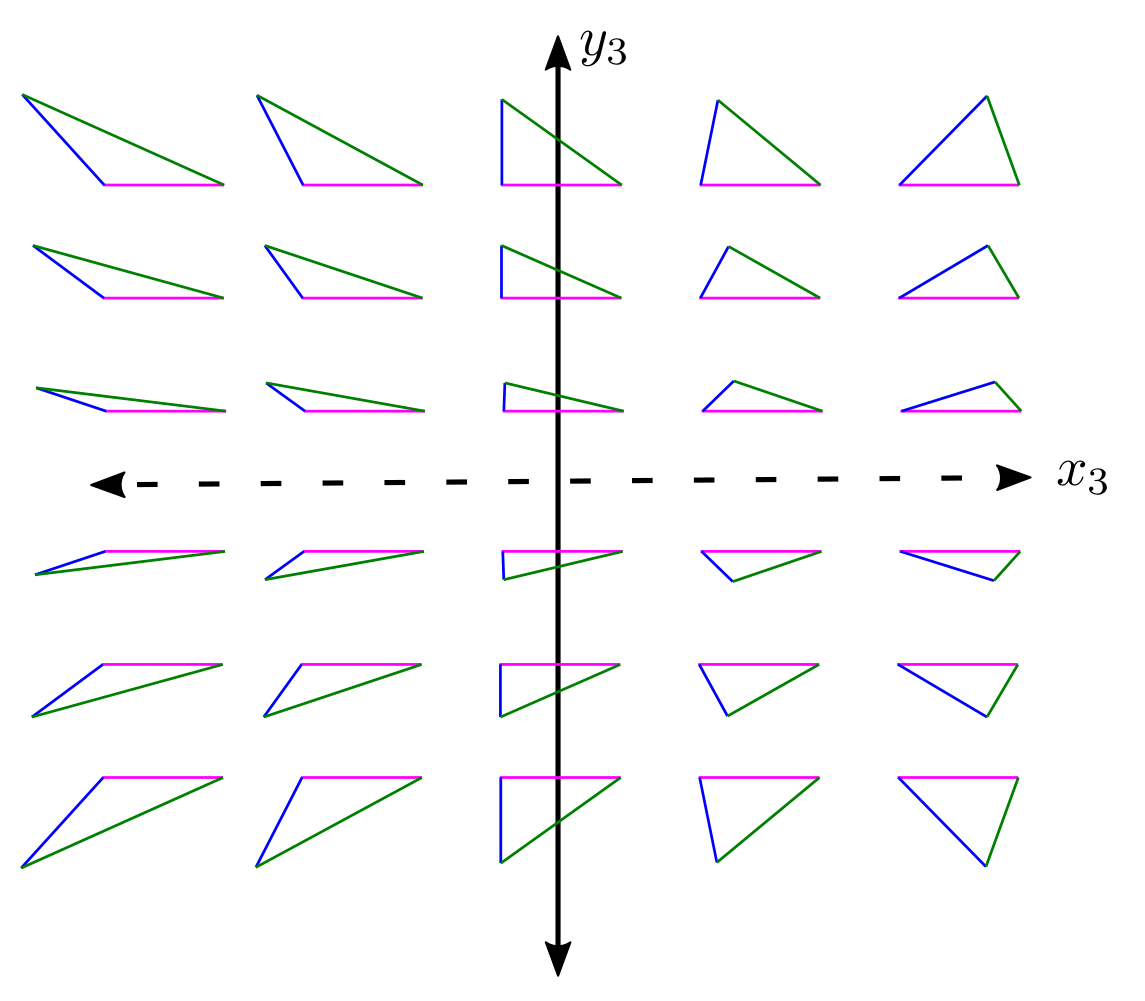
\includegraphics[width=.48\textwidth]{figures/fig-1.2.7.png}
\caption{模空间 $M$ 中 $(x_1,y_1)=(0,0)$, $(x_2,y_2)=(1,0)$ 的截面. 三角形由满足 $y_3\neq0$ 的第三个顶点 $(x_3,y_3)$ 描述. 我们为 $x_3y_3$ 平面中的一些点画出了代表三角形.}\label{src:1.2.7}
\end{figure}

\begin{example}[相似意义下带标号的三角形]\label{src:1.2.8}
定义相似意义下带标号三角形的模集合, 记作 $M^{\mathrm{lab}}$: 对象与前一个例子相同, 仍为带标号的三角形, 但等价关系改为保持标号的相似关系.
\end{example}
\begin{figure}[htbp]
\centering
\begin{tikzpicture}[scale=.7]
\draw[magenta,thick] (0,0)--(.8,1.8);
\draw[blue,thick] (.8,1.8)--(4,1.2);
\draw[green!60!black,thick] (4,1.2)--(0,0);
\node at (5.2,1.2) {$\sim$};\node at (5.2,.65) {相似};
\begin{scope}[shift={(8.7,0)},rotate=105]
\draw[magenta,thick] (0,0)--(.8,1.8);
\draw[blue,thick] (.8,1.8)--(4,1.2);
\draw[green!60!black,thick] (4,1.2)--(0,0);
\end{scope}
\node at (10.2,1.2) {$\not\sim$};\node at (10.2,.65) {不相似};
\draw[magenta,thick] (12,0)--(11.5,2.7);
\draw[blue,thick] (12,0)--(13.5,0);
\draw[green!60!black,thick] (11.5,2.7)--(13.5,0);
\end{tikzpicture}
\caption{左边的两个三角形相似, 但第三个与它们不相似.}\label{src:1.2.9}
\end{figure}
每个带标号的三角形都相似于唯一一个周长 $a+b+c=2$ 的带标号三角形. 得到描述
\begin{equation}\label{src:1.2.10}
M^{\mathrm{lab}}=\left\{(a,b,c)\;\middle|\;
\begin{aligned}
&a+b+c=2\\
&0<a<b+c\\
&0<b<a+c\\
&0<c<a+b
\end{aligned}\right\}.
\end{equation}
令 $c=2-a-b$, 便可以将 $M^{\mathrm{lab}}$ 直观呈现为 $\mathbb R^2$ 中由满足 $0<a,b<1$ 和 $a+b>1$ 的数对 $(a,b)$ 定义的解析开子集.

\begin{figure}[htbp]
\centering\begin{tikzpicture}[scale=5]
\fill[gray!25] (0,1)--(1,0)--(1,1)--cycle;
\draw[->] (0,0)--(1.12,0) node[right] {$a$};
\draw[->] (0,0)--(0,1.12) node[above] {$b$};
\draw[densely dotted] (0,1)--(1,0)--(1,1)--cycle;
\node[left] at (0,1) {$1$};\node[below] at (1,0) {$1$};
\draw[blue] (.5,.5)--(1,1);
\draw[blue] (0,1)--(1,.5);
\draw[blue] (.5,1)--(1,0);
\draw[magenta,thick,domain=0:1,samples=100] plot (\x,{(\x*\x-2*\x+2)/(2-\x)});
\draw[magenta,thick,domain=0:1,samples=100] plot ({(\x*\x-2*\x+2)/(2-\x)},\x);
\draw[magenta,thick,domain=0:1,samples=100] plot (\x,{(2-2*\x)/(2-\x)});
\fill[green!75!black] (2/3,2/3) circle (.012);
\node[font=\small,rotate=-45,fill=white,inner sep=1pt] at (.38,.55) {退化三角形};
\draw[->,gray] (1.3,.7)--(.87,.87);\node[right,font=\small] at (1.25,.73) {等腰三角形};
\draw[->,gray] (1.2,.53)--(.69,.66);\node[right,font=\small] at (1.15,.5) {等边三角形};
\draw[->,gray] (.43,.1)--(.7,{(2-2*.7)/(2-.7)});\node[below,font=\small] at (.4,.1) {直角三角形};
\end{tikzpicture}

\caption{$M^{\mathrm{lab}}$ 是阴影三角形. 品红色曲线表示由 $a^2+b^2=c^2$, $a^2+c^2=b^2$ 和 $b^2+c^2=a^2$ 定义的直角三角形, 蓝色直线表示由 $a=b$, $b=c$ 和 $a=c$ 定义的等腰三角形, 绿色点是由 $a=b=c$ 定义的唯一的等边三角形.}\label{src:1.2.11}
\end{figure}

\begin{example}[相似意义下无标号的三角形]\label{src:1.2.12}
现在转向相似意义下无标号三角形的模, 它呈现出前两个例子中未见的新特征: 对称性!
\end{example}
定义相似意义下无标号三角形的模集合, 记作 $M^{\mathrm{unl}}$: 对象是 $\mathbb R^2$ 中无标号的三角形, 等价关系为相似关系. 通过按递增次序排列边长的有序三元组 $(a,b,c)$, 可以唯一描述一个无标号三角形: 
\begin{equation}\label{src:1.2.13}
M^{\mathrm{unl}}=\left\{(a,b,c)\;\middle|\;
\begin{aligned}
&0<a\leq b\leq c<a+b\\
&a+b+c=2
\end{aligned}\right\}.
\end{equation}
\begin{figure}[H]
\centering\begin{tikzpicture}[scale=5.5]
\fill[gray!30] (0,1)--(.5,.5)--(2/3,2/3)--cycle;
\draw[->] (0,0)--(1.08,0) node[right] {$a$};
\draw[->] (0,0)--(0,1.1) node[above] {$b$};
\draw[densely dotted] (0,1)--(.5,.5);
\draw[blue] (0,1)--(2/3,2/3)--(.5,.5);
\draw[magenta,thick,domain=0:{2-sqrt(2)},samples=100] plot (\x,{(2-2*\x)/(2-\x)});
\fill[green!75!black] (2/3,2/3) circle (.012);
\foreach \v/\t in {0.5/{1/2},0.6666667/{2/3}} {
\draw (\v,0)--(\v,-.02) node[below] {$\t$};
\draw (0,\v)--(-.02,\v) node[left] {$\t$};
}
\node[left] at (0,1) {$1$};
\node[font=\small,rotate=-45,fill=white,inner sep=1pt] at (.2,.75) {退化 $a+b=c$};
\node[font=\small,rotate=-27,above] at (.25,.9) {等腰 $b=c$};
\node[font=\small,rotate=45,below] at (.59,.57) {等腰 $a=b$};
\draw[->,gray] (.93,.86)--(.68,.68);\node[right,font=\small] at (.8,.89) {等边};
\draw[->] (.16,.25)--(.43,{(2-2*.43)/(2-.43)});
\node[font=\small,align=center] at (.17,.18) {直角三角形\\$a^2+b^2=c^2$};
\end{tikzpicture}

\caption{$M^{\mathrm{unl}}$ 的图像.}\label{src:1.2.14}
\end{figure}
满足 $a=b$ 或 $b=c$ 的等腰三角形, 以及满足 $a=b=c$ 的等边三角形, 其对称群分别为 $\mathbb Z/2$ 和 $S_3$. 遗憾的是, 上述 $M^{\mathrm{unl}}$ 的描述并未编码这一信息. 注意, 在 $S_3$ 对标号的自然作用下, 可以把 $M^{\mathrm{unl}}$ 等同于商 $M^{\mathrm{lab}}/S_3$; 而等腰三角形和等边三角形的稳定子, 恰好就是其对称群 $\mathbb Z/2$ 和 $S_3$. 在既非等腰又非等边的三角形轨迹上, $S_3$ 的作用是自由的.

% Source printed pp. 16-28, entire Section 1.3.
\section{函子观点}\label{src:1.3}
\begin{epigraph}
数学对象由它们与同类的所有其他对象之间的关系网络所决定, 也通过这一网络得到理解.
\epigraphauthor{Barry Mazur~\cite{Maz08}}
\end{epigraph}
定义一个\newterm{模函子}{moduli functor}, 需要明确: 
\begin{enumerate}[(1)]
\item 对象的族; 
\item 两个对象族在什么情形下等价; 以及
\item 对象族如何沿态射拉回.
\end{enumerate}
在代数范畴中, 这些数据汇集为一个反变函子
\begin{equation}\label{src:1.3.1}
F:\Sch\longrightarrow\Sets,\qquad S\longmapsto\{S\text{ 上的对象族}\},
\end{equation}
其中, 对映射 $f:S\to T$, $F(f):F(T)\to F(S)$ 给出从 $T$ 上的族到 $S$ 上的族的拉回映射, 有时简记为 $f^*$.(要成为函子, 拉回映射必须与复合相容: 对映射 $f:S\to T$ 和 $g:T\to U$, 有 $F(g\circ f)=F(f)\circ F(g)$.)

\subsection{族的重要性}\label{src:1.3.1-subsection}
通过族, 我们能够精确表述模空间 $M$. 空间 $S$ 上的对象族 $\mathcal C$ 定义一个集合映射
\begin{equation}\label{src:1.3.2}
S\longrightarrow M,\qquad s\longmapsto[\mathcal C_s],
\end{equation}
其中, 纤维 $[\mathcal C_s]\in M$ 是 $\mathcal C$ 沿包含映射 $\{s\}\hookrightarrow S$ 的拉回. 在拓扑范畴(相应地, 在代数范畴)中, 我们希望映射 $S\to M$ 连续(相应地, 为代数映射). 理想情况下, $S$ 上的族与态射 $S\to M$ 一一对应; 换言之, 空间 $M$ 表出~\eqref{src:1.3.1}~中的函子 $F$. 如果如此, 我们称 $M$ 为细模空间; 不过很快就会看到, 这往往是过高的奢望.

通过族来定义模空间有如下优点: 
\begin{itemize}
\item 可以赋予模集合 $M$ 更丰富的结构. 要给 $M$ 赋予拓扑, 我们规定: 子集 $U\subseteq M$ 为开集, 当且仅当对每个 $S$ 上的对象族 $\mathcal C$, 集合 $\{s\in S\mid[\mathcal C_s]\in U\}$ 都是 $S$ 的开子集. $M$ 上的整体函数 $f$ 可以定义为一组数据: 对每个 $S$ 上的族 $\mathcal X$, 给定 $S$ 上的整体函数 $f_{\mathcal X}$, 且这些函数彼此相容.
\item 当 $M$ 为细模空间时, 恒等映射 $\mathrm{id}:M\to M$ 对应于模空间 $M$ 上的一个对象族 $\mathcal U$. 这就是\newterm{万有族}{universal family}: 对任意其他 $S$ 上的族 $\mathcal C$, 存在唯一态射 $S\to M$(其集合映射由~\eqref{src:1.3.2}~给出), 使万有族 $\mathcal U$ 拉回为 $\mathcal C$.
\end{itemize}
这无疑是抽象程度上的巨大飞跃!而且看起来我们似乎只是让事情更难了: 我们不再通过指定空间的点, 拓扑以及可能具有的复结构或代数结构来引入空间, 而必须指定大量范畴数据. 然而, 实践中通常很容易定义性质良好的族的概念. Yoneda 引理(\bookref{1.3.12})确立了这种观点的转变: 到一个空间的映射所组成的函子, 唯一决定该空间.

\begin{example}[带标号三角形的族]\label{src:1.3.3}
回到例~\bookref{1.2.8}~中引入的带标号三角形在相似关系下的模, 我们将拓扑空间 $S$ 上的\textit{带标号三角形的族}定义为一个元组 $(\mathcal T,\sigma_1,\sigma_2,\sigma_3)$, 其中 $\mathcal T\to S$ 是一个带有三个截面 $\sigma_i:S\to\mathcal T$ 的纤维丛, 配备连续距离函数 $d:\mathcal T\times_S\mathcal T\to\mathbb R_{\geq0}$. 要求对每个点 $s\in S$, 限制 $d_s:\mathcal T_s\times\mathcal T_s\to\mathbb R_{\geq0}$ 是纤维 $\mathcal T_s$ 上的度量, 并使 $\mathcal T_s$ 等距于一个以 $\sigma_i(s)$ 为顶点的三角形.

称 $S\in\mathsf{Top}$ 上的两个带标号三角形族 $(\mathcal T,(\sigma_i))$ 和 $(\mathcal T',(\sigma_i'))$ \textit{相似}, 是指存在 $S$ 上的同胚 $f:\mathcal T\to\mathcal T'$, 与截面相容(即 $f\circ\sigma_i=\sigma_i'$), 并且对每个 $s\in S$, 所诱导的纤维间映射 $\mathcal T_s\to\mathcal T'_s$ 是三角形的相似变换, 即重新缩放后为等距映射. 给定带标号三角形族 $\mathcal T\to S$ 和连续映射 $S'\to S$, 拉回族定义为集合的纤维积 $\mathcal T\times_S S'$, 配备拉回截面 $\sigma'_i:S'\to\mathcal T'$ 及所继承的距离函数.
\end{example}
\begin{figure}[htbp]
\centering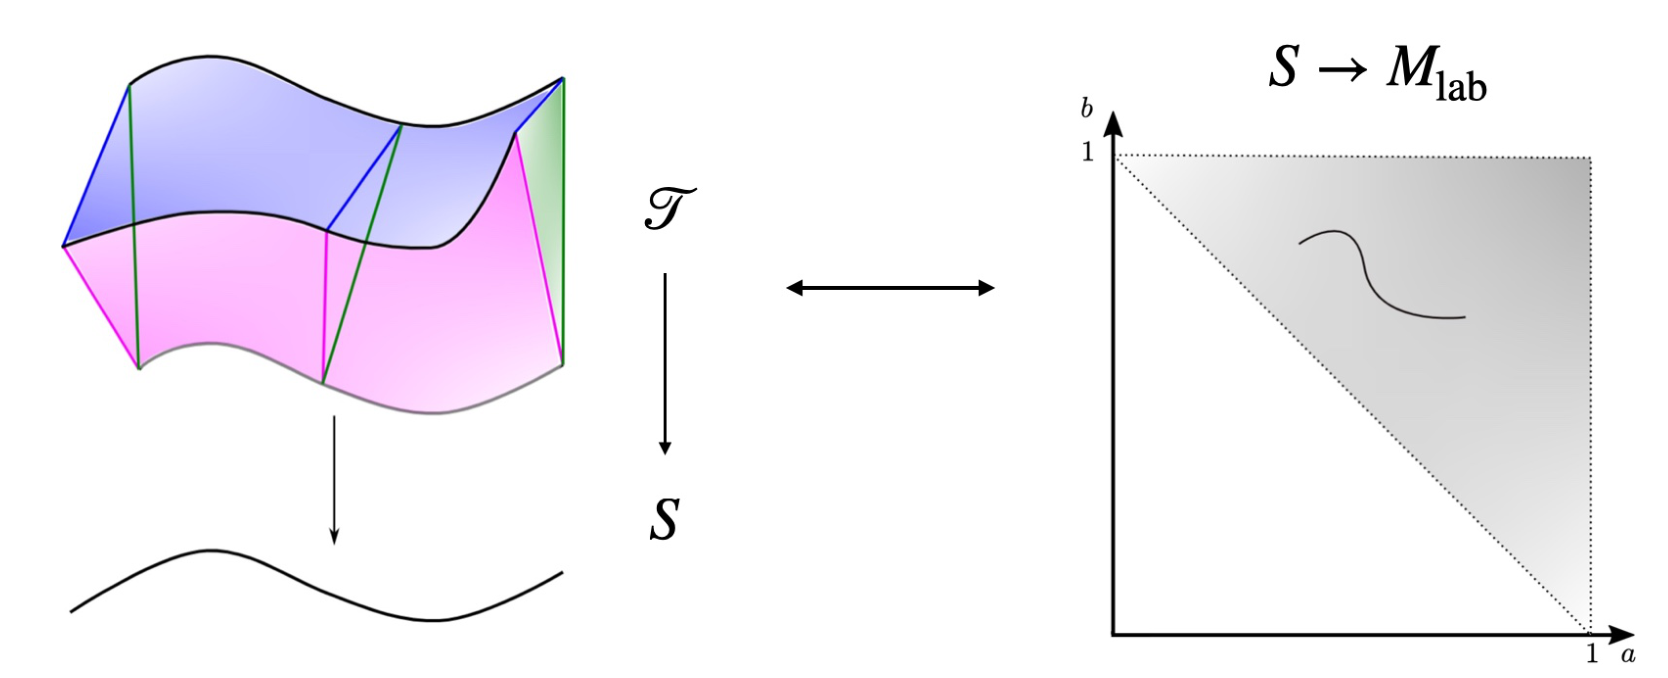
\includegraphics[width=.76\textwidth]{figures/fig-1.3.4.png}
\caption{曲线上的带标号三角形族对应于模空间中的一条弧.}\label{src:1.3.4}
\end{figure}
我们定义带标号三角形的模函子为
\[
\begin{aligned}
F_{M^{\mathrm{lab}}}:&\ \mathsf{Top}\longrightarrow\Sets,\\
&S\longmapsto\{S\text{ 上的带标号三角形族 }(\mathcal T\to S,\sigma_i)\}/(\text{相似}).
\end{aligned}
\]
回忆~\eqref{src:1.2.10}, 将三角形送到其边长的对应, 给出 $F_{M^{\mathrm{lab}}}$ 与下列集合之间的双射: 
\[
M^{\mathrm{lab}}=
\left\{(a,b,c)\ \middle|\
\begin{aligned}
a+b+c&=2\\
0<a&<b+c\\
0<b&<a+c\\
0<c&<a+b
\end{aligned}\right\}.
\]
由于这对每个拓扑空间 $S$ 都延拓为彼此相容的同构
$F_{M^{\mathrm{lab}}}(S)\to\operatorname{Mor}(S,M^{\mathrm{lab}})$, 拓扑空间 $M^{\mathrm{lab}}$ 表出函子 $F_{M^{\mathrm{lab}}}$. 因而存在万有族 $\mathcal T_{\mathrm{univ}}\to M^{\mathrm{lab}}$, 以及截面 $\sigma_i:M^{\mathrm{lab}}\to\mathcal T_{\mathrm{univ}}$.
\begin{figure}[htbp]
\centering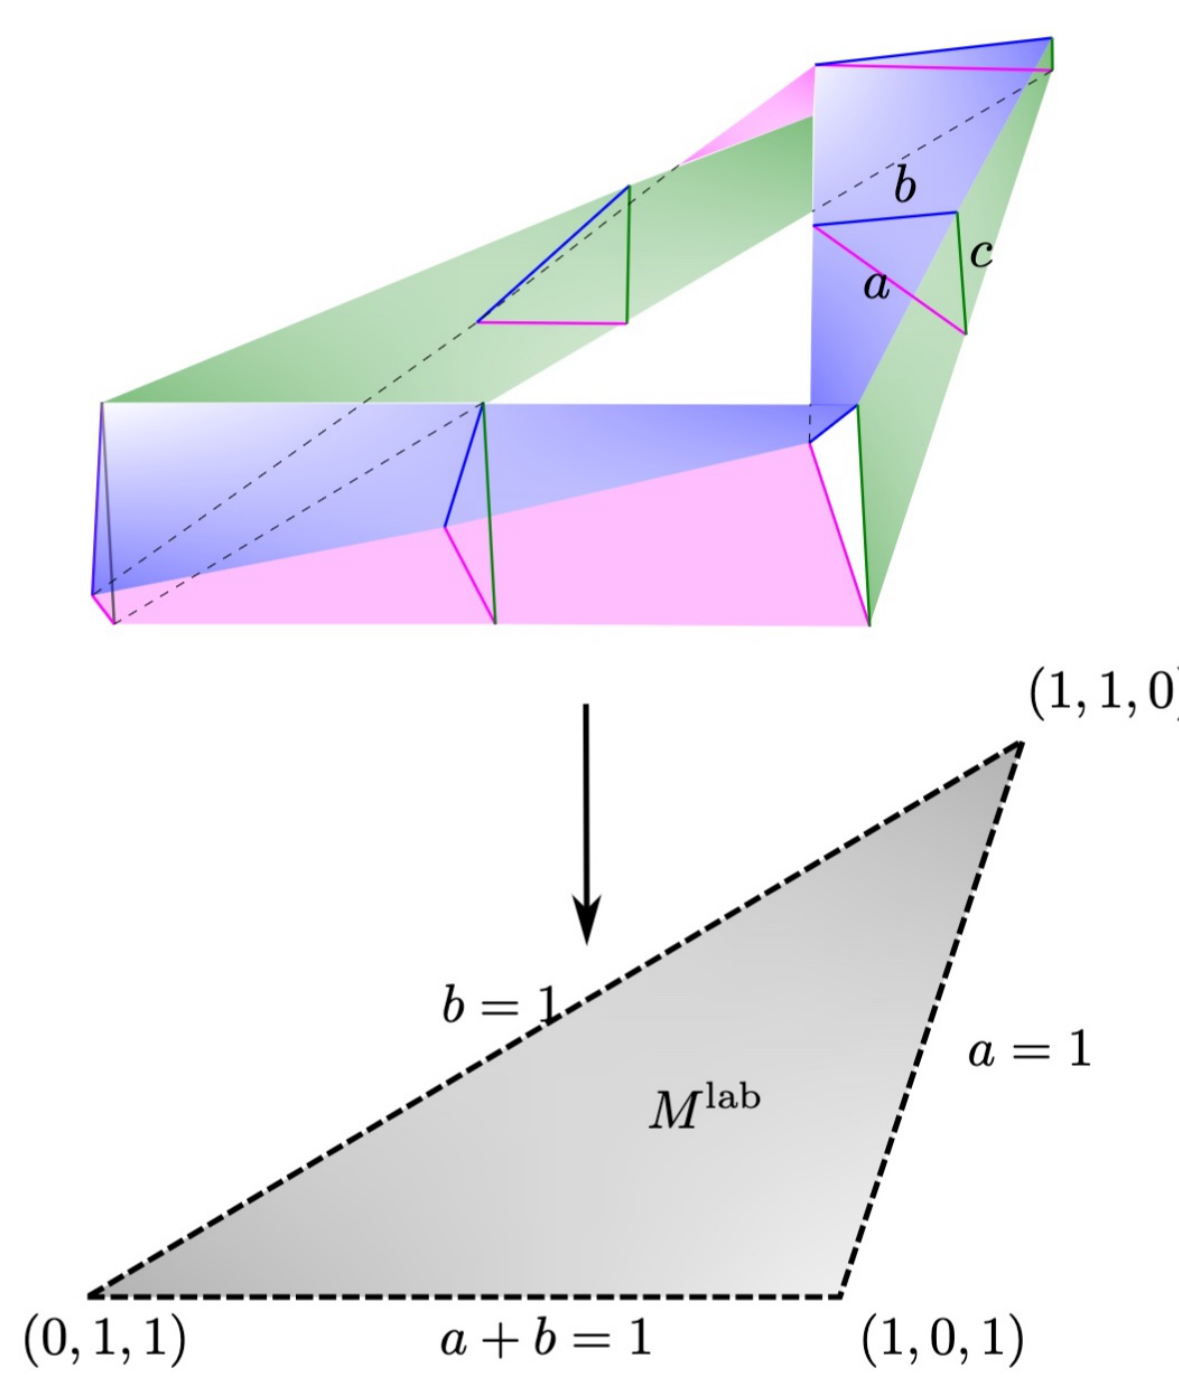
\includegraphics[width=.52\textwidth]{figures/fig-1.3.5.png}
\caption{相似关系下带标号三角形的万有族 $U^{\mathrm{lab}}\to M^{\mathrm{lab}}$.}\label{src:1.3.5}
\end{figure}

\begin{example}[无标号三角形的族]\label{src:1.3.6}
回到例~\bookref{1.2.12}, 我们将\textit{无标号三角形的族}定义为一个纤维丛 $\mathcal T\to S$, 配备连续距离函数 $d:\mathcal T\times_S\mathcal T\to\mathbb R_{\geq0}$, 其在每个纤维上的限制都是度量, 且每个纤维都等距于一个三角形. 两个族 $\mathcal T\to S$ 和 $\mathcal T'\to S$ \textit{相似}, 是指存在 $S$ 上与截面相容的同胚 $f:\mathcal T\to\mathcal T'$, 在各纤维上诱导三角形的相似变换.

我们定义函子
\[
\begin{aligned}
F_{M^{\mathrm{unl}}}:&\ \mathsf{Top}\longrightarrow\Sets,\\
&S\longmapsto\{S\text{ 上的无标号三角形族}\}/(\text{相似}),
\end{aligned}
\]
但已经可以看出, 对象的对称性带来了复杂情况: 每个等边三角形的对称群为 $S_3$, 等腰三角形的对称群则为 $\mathbb Z/2$. 根据命题~\bookref{1.3.30}, 这个函子不可表, 因为存在三角形的非平凡族 $\mathcal T$, 其所有纤维都是相似的三角形. 例如, 利用等边三角形的一个对称变换粘合两个平凡族, 可以构造 $S^1$ 上的一个非平凡三角形族.
\end{example}
\begin{figure}[htbp]
\centering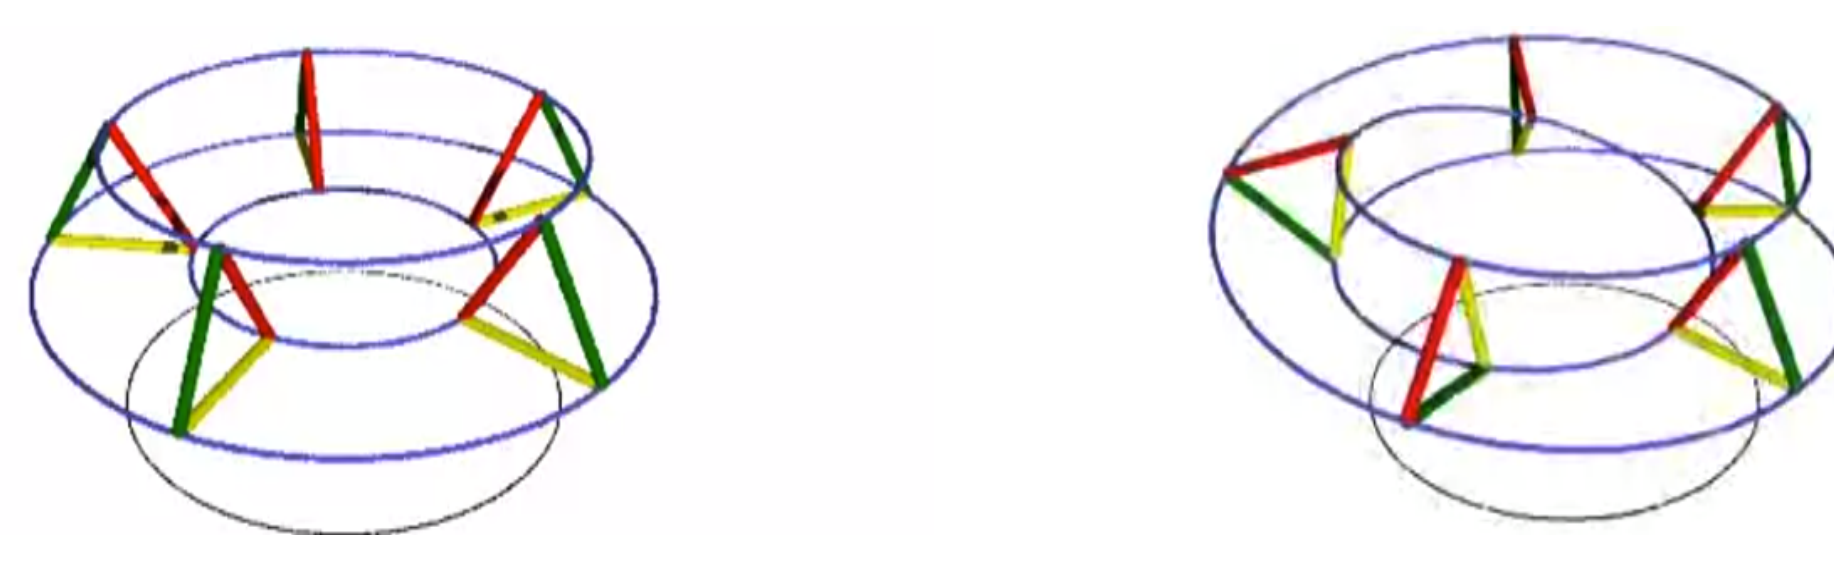
\includegraphics[width=.8\textwidth]{figures/fig-1.3.7.png}
\caption{等边三角形的平凡族(左)与非平凡族(右). 图像取自 Jonathan Wise 制作的视频, 见 \url{http://math.colorado.edu/~jonathan.wise/visual/moduli/index.html}.}\label{src:1.3.7}
\end{figure}

\subsection{曲线, 向量丛与轨道的模函子}\label{src:1.3.2-subsection}
在 $\mathbb C$-概形范畴中定义一个模函子 $F:\Sch/\mathbb C\to\Sets$, 意味着要对每个 $\mathbb C$-概形 $S$, 指定一个由 $S$ 上的对象族组成的集合 $F(S)$; 并对每个 $\mathbb C$-概形态射 $S'\to S$, 指定拉回映射 $F(S)\to F(S')$, 且这些拉回映射与复合相容.

为了获得关于模函子的直观认识, 代入特殊的测试概形总是有益的. 例如, 代入 $S=\operatorname{Spec}\mathbb C$, 就得到由对象组成的底层模集合 $F(\operatorname{Spec}\mathbb C)$. 代入 $S=\mathbb C[\epsilon]/(\epsilon^2)$, 就得到一个二元组的集合, 每个二元组由一个 $\mathbb C$-点和一个切向量组成; 代入一条曲线(或一个离散赋值环), 则得到该曲线上的对象族.

\begin{example}[光滑曲线的模函子]\label{src:1.3.8}
\textit{亏格为 $g$ 的光滑曲线族}是一个光滑, 固有的概形态射 $\mathcal C\to S$, 使得对每个 $s\in S$, 纤维 $\mathcal C_s$ 都是亏格为 $g$ 的连通(光滑固有)曲线.

亏格为 $g$ 的光滑曲线的模函子为
\[
\begin{aligned}
F_{M_g}:&\ \Sch/\mathbb C\longrightarrow\Sets,\\
&S\longmapsto\{\text{亏格为 }g\text{ 的光滑曲线族 }\mathcal C\to S\}/\sim,
\end{aligned}
\]
其中, 两个族 $\mathcal C\to S$ 和 $\mathcal C'\to S$ 等价, 是指存在 $S$ 上的同构 $\mathcal C\to\mathcal C'$. 如果 $S'\to S$ 是一个 $\mathbb C$-概形映射, $\mathcal C\to S$ 是曲线族, 则拉回定义为族 $\mathcal C\times_S S'\to S'$.
\end{example}
\begin{figure}[htbp]
\centering
\begin{tikzpicture}
\node[anchor=south west,inner sep=0] (art) at (0,0) {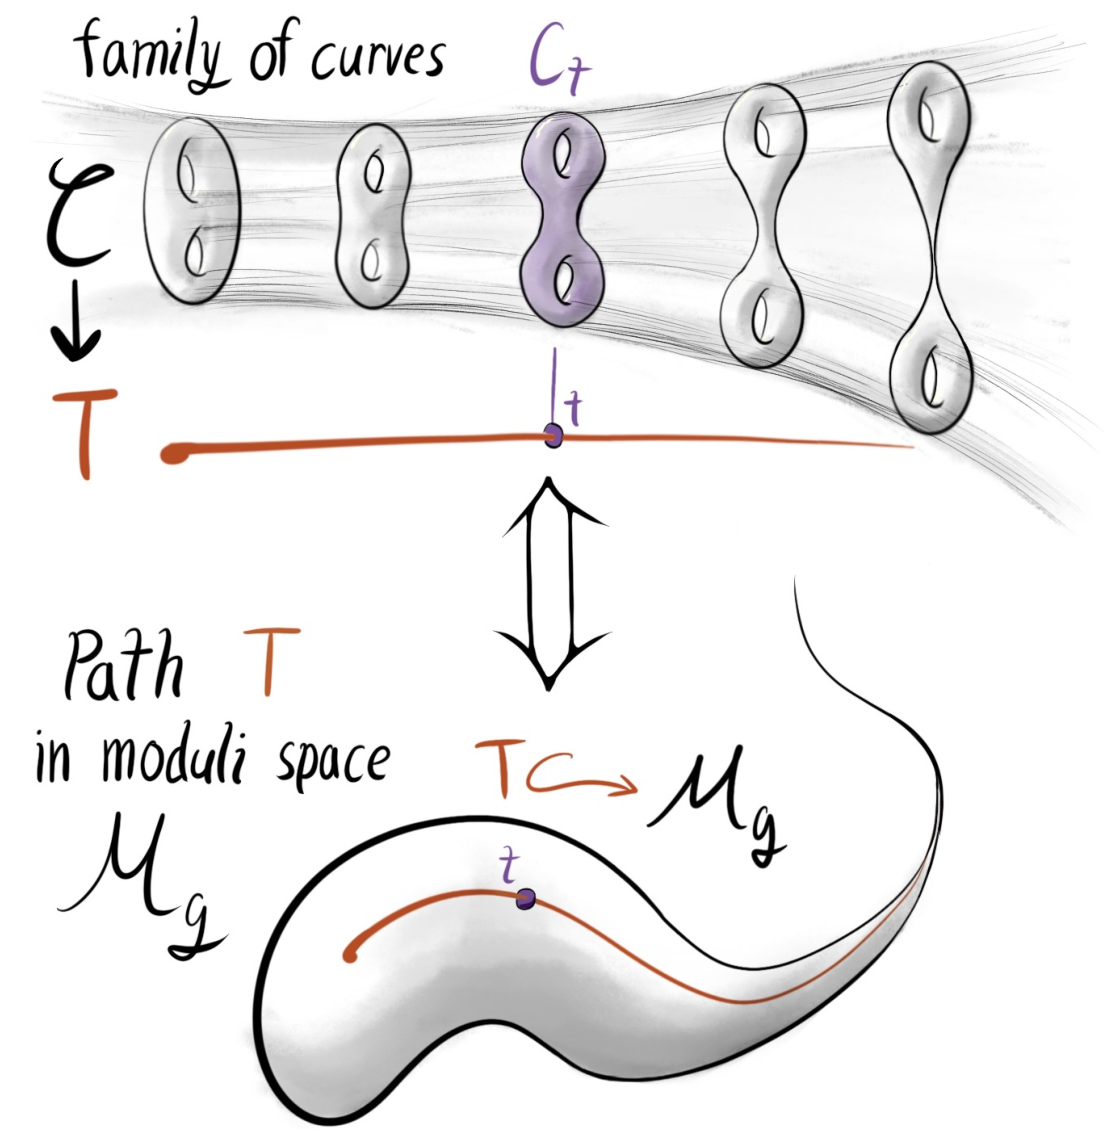
\includegraphics[width=.5\textwidth]{figures/fig-1.3.9.png}};
\begin{scope}[x={(art.south east)},y={(art.north west)}]
\fill[white] (.02,.905) rectangle (.42,1);
\node[font=\small] at (.22,.952) {曲线族};
\fill[white] (.02,.29) rectangle (.38,.47);
\node[font=\small,align=center] at (.20,.38) {模空间\\中的路径};
\end{scope}
\end{tikzpicture}
\caption{曲线族(图中画为 Riemann 曲面)与模空间中的路径之间的对应. 图中还展示了光滑曲线的模空间 $M_g$ 不是紧的: 当路径趋近模空间的边界时, 曲线退化为一条奇异的结点曲线. 后面将看到, 稳定曲线的模空间 $\overline M_g$ 是紧的(定理~\bookref{6.5.23}).}\label{src:1.3.9}
\end{figure}

\begin{example}[曲线上向量丛的模函子]\label{src:1.3.10}
令 $C$ 为 $\mathbb C$ 上一条固定的光滑, 连通射影曲线. $\mathbb C$-概形 $S$ 上的\textit{秩为 $r$, 次数为 $d$ 的向量丛族}, 是 $C\times S$ 上的一个向量丛 $\mathcal E$, 使对每个 $s\in S$, $\mathcal E$ 在 $C_{\kappa(s)}:=C\times_{\mathbb C}\kappa(s)$ 上的限制 $\mathcal E_s:=\mathcal E|_{C_{\kappa(s)}}$ 的秩为 $r$, 次数为 $d$. $C$ 上秩为 $r$, 次数为 $d$ 的向量丛的模函子为
\[
\Sch/\mathbb C\longrightarrow\Sets,\qquad
S\longmapsto
\left\{\begin{gathered}
C\times S\text{ 上的向量丛 }\mathcal E\\
\text{其秩为 }r\text{, 次数为 }d
\end{gathered}\right\}/(\text{同构}).
\]
如果 $f:S'\to S$ 是一个 $\mathbb C$-概形映射, $\mathcal E$ 是 $C\times S$ 上的向量丛, 则拉回定义为 $C\times S'$ 上的向量丛 $(\mathrm{id}\times f)^*\mathcal E$.
\end{example}
我们将在第~\bookref{1.3.5-subsection}~小节看到, 这两个函子都不可表, 相应地, 也都不存在细模空间.

\begin{example}[轨道的模函子]\label{src:1.3.11}
考虑 $\mathbb C$ 上的代数群 $G$ 在 $\mathbb C$-概形 $X$ 上的作用. 对每个 $\mathbb C$-概形 $S$, 抽象群 $G(S)$ 在集合 $X(S)$ 上作用; 事实上, 给出这样的作用, 并使其关于 $S$ 具有函子性, 就唯一确定了该群作用(习题~\bookref{B.1.11}). 我们可以考虑函子
\[
\Sch/\mathbb C\longrightarrow\Sets,\qquad S\longmapsto X(S)/G(S).
\]
这是商的模函子的一个十分朴素的候选, 即使对自由作用, 也远远不能做到可表(见习题~\bookref{1.3.38}). 我们将在 \S\bookref{1.6.5-subsection} 中修改这个例子.
\end{example}
某些情况下, 你可能确切知道要参数化哪些对象, 但引入族的概念未必容易. 对对象族也可能有几个候选概念, 它们可能在同一个拓扑空间上给出不同的概形结构. 高维簇的模就是这样的例子(见 \S\bookref{10.1.3-subsection}).

\subsection{Yoneda 引理与可表函子}\label{src:1.3.3-subsection}
\begin{epigraph}
Yoneda 引理是数学中最难的平凡事实.
\epigraphauthor{Dan Piponi}
\end{epigraph}
遵循 Grothendieck 的思想, 我们将通过研究到概形 $X$ 的所有映射来研究 $X$!这个思维上的技巧正是函子方法的核心: 一个几何对象由它与所有其他对象之间的关系所决定. Yoneda 引理将此严格化: 对范畴 $\mathcal C$ 的一个对象 $X$, 反变函子
\[
h_X:\mathcal C\longrightarrow\Sets,\qquad S\longmapsto\operatorname{Mor}(S,X)
\]
恢复对象 $X$ 本身.

\begin{lemma}[Yoneda 引理]\label{src:1.3.12}
令 $\mathcal C$ 为一个范畴, $X$ 为其中一个对象. 对每个反变函子 $G:\mathcal C\to\Sets$, 映射
\[
\operatorname{Mor}(h_X,G)\longrightarrow G(X),\qquad
\alpha\longmapsto\alpha_X(\mathrm{id}_X)
\]
为双射, 且关于 $X$ 和 $G$ 都具有函子性. 这里, 左边表示自然变换 $h_X\to G$ 的集合, $\alpha_X$ 表示映射 $h_X(X)=\operatorname{Mor}(X,X)\to G(X)$.
\end{lemma}
\begin{exercise}[一生中至少应做一次]\label{src:1.3.13}
证明 Yoneda 引理. 为此, 必须准确说明``关于 $X$ 和 $G$ 都具有函子性''的含义.
\end{exercise}
\begin{caution}\label{src:1.3.14}
全书中, 我们将一贯滥用记号, 不区分元素 $g\in G(X)$ 与对应的态射 $h_X\to G$; 后者又常简写为 $X\to G$.
\end{caution}
\begin{definition}[可表函子与细模空间]\label{src:1.3.15}
称函子 $F:\Sch\to\Sets$ \newterm{可由概形表出}{representable by a scheme}, 是指存在概形 $X$ 和函子同构 $F\xrightarrow{\sim}h_X$.

当 $F$ 为模函子, 且可由概形 $M$ 表出时, 称 $M$ 为\newterm{细模空间}{fine moduli space}.
\end{definition}
由 Yoneda 引理(\bookref{1.3.12}), 如果一个函子可表, 那么它可由唯一的概形表出. 我们的一个目标, 就是理解给定的模函子 $F$ 何时具有细模空间, 即何时可由概形表出.

\begin{example}[射影空间作为函子]\label{src:1.3.16}
由~\cite[定理 II.7.1]{Har77}, 存在具有函子性的双射
\[
\operatorname{Mor}(S,\mathbb P^n_{\mathbb Z})\cong
\left\{(L,s_0,\ldots,s_n)\ \middle|\
\begin{gathered}
L\text{ 是 }S\text{ 上的线丛, 由截面}\\
s_0,\ldots,s_n\in\Gamma(S,L)\text{ 整体生成}
\end{gathered}\right\}/\sim,
\]
其中, $(L,s_i)\sim(L',s'_i)$ 是指存在同构 $\alpha:L\to L'$, 使对所有 $i$ 都有 $s_i=\alpha^*s'_i$. 换言之, 右边的函子可由概形 $\mathbb P^n_{\mathbb Z}$ 表出. 截面 $s_i$ 整体生成这一条件, 意味着对每个 $x\in S$, 至少有一个截面 $s_i(x)\in L\otimes\kappa(x)$ 非零; 等价地, $(s_0,\ldots,s_n):\mathcal O_S^{\oplus n+1}\to L$ 为满射.
\end{example}

\begin{example}[Grassmann 函子]\label{src:1.3.17}
作为集合, Grassmann 簇 $\operatorname{Gr}(q,n)$ 参数化 $n$ 维空间的 $q$ 维商.\footnote{也可以将这些点视为 $q$ 维子空间, 但在本讲义中, 我们遵循 Grothendieck 使用商的约定.} 然而, 概形 $S$ 上的 $q$ 维商的族是什么?一个朴素的猜测可能是商 $p:\mathcal O_S^n\twoheadrightarrow\mathcal O_S^k$, 但这根本不可能可表(见习题~\bookref{1.3.38}). 射影空间的情形提示我们将 \newterm{Grassmann 函子}{Grassmannian functor}定义为
\[
\begin{aligned}
\operatorname{Gr}(q,n):&\ \Sch\longrightarrow\Sets,\\
&S\longmapsto
\left\{[\mathcal O_S^{\oplus n}\twoheadrightarrow Q]\ \middle|\ Q\text{ 为秩 }q\text{ 的向量丛}\right\}/\sim,
\end{aligned}
\]
其中, $[p:\mathcal O_S^{\oplus n}\twoheadrightarrow Q]\sim[p':\mathcal O_S^{\oplus n}\twoheadrightarrow Q']$, 是指存在同构 $\Psi:Q\xrightarrow{\sim}Q'$ 使图
\[
\begin{tikzcd}
\mathcal O_S^{\oplus n}\arrow[r,"p"]\arrow[dr,"p'"'] & Q\arrow[d,"\Psi","\sim"']\\
&Q'
\end{tikzcd}
\]
交换(即 $p'=\Psi\circ p$); 等价地, $\ker(p)=\ker(p')$. 拉回以自然方式定义.

后面我们将证明, $\operatorname{Gr}(q,n)$ 可由一个在 $\mathbb Z$ 上射影的概形表出(定理~\bookref{2.1.1}). 这一结果的证明很好地说明了函子方法的用处, 也是 Hilb 和 Quot 可表性(定理~\bookref{2.1.2}~和~\bookref{2.1.3})的热身.
\end{example}
以下习题将帮助你练习函子方法.

\begin{exercise}[仿射空间与射影空间]\label{src:1.3.18}
令 $S$ 为概形, $E$ 为 $S$ 上的向量丛.
\begin{enumerate}[(a)]
\item 证明仿射空间 $\mathbb A(E):=\mathcal{S}pec_S(\operatorname{Sym}^*E)$ 表出将 $f:T\to S$ 送到 $\Gamma(T,f^*E^\vee)$ 的函子, 其中 $E^\vee:=\mathcal{H}om_{\mathcal O_S}(E,\mathcal O_S)$. 注意, $\mathbb A(E)$ 的一个 $\Bbbk$-点是 $E\otimes_{\mathcal O_S}\Bbbk$ 的对偶中的一个元素.\footnote{这与~\cite[习题 5.18, 162 页的定义]{Har77}, \cite[II.4.1.1]{EGA}~以及~\cite[Tag 01OB]{SP}~一致; 但须注意, 有些作者在定义 $\mathbb A(E)$ 和 $\mathbb P(E)$ 时, 使用对偶 $E^\vee$ 而非 $E$.} 还应注意特殊情形 $\mathbb A(\mathcal O_S^{\oplus n})\cong\mathbb A_S^n$.
\item 证明 $E$ 的射影化 $\mathbb P(E):=\mathcal{P}roj_S(\operatorname{Sym}^*E)$ 表出函子
\[
\begin{aligned}
\Sch/S&\longrightarrow\Sets,\\
(T\xrightarrow{f}S)&\longmapsto
\{q:f^*E\twoheadrightarrow L\text{, 其中 }L\text{ 为 }T\text{ 上的线丛}\}/\sim,
\end{aligned}
\]
其中, $[q:f^*E\twoheadrightarrow L]\sim[q':f^*E\twoheadrightarrow L']$ 是指 $\ker(q)=\ker(q')$(等价地, 存在同构 $\alpha:L\to L'$, 使 $q'=\alpha\circ q$). 注意, $E$ 自然等同于 $\mathcal O_{\mathbb P(E)}(1)$ 沿 $\mathbb P(E)\to S$ 的推前; 当 $E$ 平凡时, 有等同 $\mathbb P(\mathcal O_S^{n+1})\cong\mathbb P^n$.
\end{enumerate}
\end{exercise}
\begin{exercise}[简单, 适于练习]\label{src:1.3.19}
给出以下对象的函子描述: 
\begin{enumerate}[(a)]
\item $\mathbb A^n\setminus0$; 
\item $\operatorname{Spec}\Bbbk[x_1,\ldots,x_n]/(f_1,\ldots,f_m)$; 
\item $\mathcal{S}pec_S\mathcal A$, 其中 $\mathcal A$ 是概形 $S$ 上的拟凝聚代数层; 以及
\end{enumerate}
\end{exercise}
\begin{exercise}[困难]\label{src:1.3.20}
若 $S$ 为概形, $\mathcal A$ 为正分次 $\mathcal O_S$-代数, 给出 $\mathcal{P}roj_S\mathcal A$ 的函子描述.(另见~\cite[Tag 01NS]{SP}.)
\end{exercise}
\begin{exercise}[中等, 适于练习]\label{src:1.3.21}
令 $X$ 为概形, $F_1$ 和 $F_2$ 为 $X$ 上的向量丛. 证明函子
\[
\begin{aligned}
\underline{\mathcal{H}om}_{\mathcal O_X}(F_1,F_2):&\ \Sch/X\longrightarrow\Sets,\\
&(f:T\to X)\longmapsto\operatorname{Hom}_{\mathcal O_T}(f^*F_1,f^*F_2)
\end{aligned}
\]
可由 $\mathbb A(\mathcal{H}om_{\mathcal O_X}(F_1,F_2)^\vee)\to X$ 表出.

注意以下记号的区别: 
\begin{itemize}
\item $\operatorname{Hom}_{\mathcal O_X}(F_1,F_2)$: $\mathcal O_X$-模同态群; 
\item $\mathcal{H}om_{\mathcal O_X}(F_1,F_2)$: $\mathcal O_X$-模同态层; 
\item $\underline{\mathcal{H}om}_{\mathcal O_X}(F_1,F_2)$: 参数化 $\mathcal O_X$-模同态的函子或概形.
\end{itemize}
\end{exercise}
\begin{exercise}[中等]\label{src:1.3.22}
令 $X$ 为域 $\Bbbk$ 上的概形, $F_1$ 和 $F_2$ 为 $X$ 上的向量丛. 证明从仿射 $\Bbbk$-概形范畴出发的函子
\[
\begin{aligned}
\underline{\operatorname{Ext}}^1_{\mathcal O_X}(F_1,F_2):&\
\mathsf{AffSch}/\Bbbk\longrightarrow\Sets,\\
&T\longmapsto\operatorname{Ext}^1_{\mathcal O_{X\times T}}(p_1^*F_1,p_1^*F_2)
\end{aligned}
\]
可由 $\mathbb A(\operatorname{Ext}^1_{\mathcal O_X}(F_1,F_2)^\vee)$ 表出. 另见~\cite[\S7.3]{LP97}~和命题~\bookref{9.2.13}.
\end{exercise}
\begin{exercise}[中等]\label{src:1.3.23}
令 $S$ 为 Noether 概形, $E\to F$ 为 $\mathbb P_S^n$ 上的凝聚层同态, 其中 $F$ 在 $S$ 上平坦. 证明由下式定义的 $S$ 的子函子(更准确地说, 是 $h_S=\operatorname{Mor}(-,S)$ 的子函子)
\[
\Sch\longrightarrow\Sets,\qquad
T\longmapsto\{T\to S\text{ 的态射, 使 }E_T\to F_T\text{ 为零}\}
\]
可由 $X$ 的一个闭子概形表出.
\end{exercise}
\begin{exercise}[Weil 限制, 困难]\label{src:1.3.24}
设 $S'\to S$ 为概形态射. 态射 $X'\to S'$ 的 \newterm{Weil 限制}{Weil restriction}是函子
\[
\operatorname{Re}_{S'/S}(X'):\Sch/S\longrightarrow\Sets,\qquad
(T\to S)\longmapsto X'(T\times_S S').
\]
\begin{enumerate}[(1)]
\item 若 $\Bbbk/\Bbbk'$ 为次数 $d$ 的域扩张, 证明 $\operatorname{Re}_{\Bbbk'/\Bbbk}\mathbb A^1\cong\mathbb A^d$.
\item 证明 $T:=\operatorname{Re}_{\mathbb C/\mathbb R}(\mathbb G_{m,\mathbb C})$ 为 $\mathbb R$ 上的代数群, 它是秩为 $2$ 的非分裂环面, 即 $T\times_{\mathbb R}\mathbb C\cong\mathbb G_{m,\mathbb C}^2$, 但 $T\not\cong\mathbb G_{m,\mathbb R}^2$.
\item (困难)假设 $S'\to S$ 有限且平坦, 并且对每个 $s\in S$, 纤维 $X'_s$ 中的任意有限点集都包含于一个仿射开集内, 则 $\operatorname{Re}_{S'/S}(X')$ 可表. 另见~\cite[定理 $7.4$]{BLR90}.
\end{enumerate}
\end{exercise}

\subsection{万有族}\label{src:1.3.4-subsection}
\begin{definition}\label{src:1.3.25}
若 $F:\Sch\to\Sets$ 为模函子, 且通过函子同构 $\alpha:F\xrightarrow{\sim}h_M$ 可由概形 $M$ 表出, 则 $F$ 的\textit{万有族}是对象 $u\in F(M)$, 它在 $\alpha$ 下对应于恒等态射 $\mathrm{id}_M\in h_M(M)=\operatorname{Mor}(M,M)$.
\end{definition}
\begin{exercise}[简单但重要]\label{src:1.3.26}
令 $F:\Sch\to\Sets$ 为可由概形 $M$ 表出的函子, $u\in F(M)$ 为万有族. 若 $a\in F(T)$ 为概形 $T$ 上的一个对象, 对应于映射 $f_a:T\to M$, 证明对象 $a$ 为 $u$ 沿 $f_a$ 的拉回, 即 $a=F(f_a)(u)$.
\end{exercise}
暂且放下疑虑, 假设确实存在一个概形 $M_g$, 表出亏格为 $g$ 的光滑曲线的模函子(例~\bookref{1.3.8}). 那么恒等映射 $M_g\to M_g$ 就对应于一个亏格为 $g$ 的曲线族 $U_g\to M_g$, 满足以下万有性质: 对概形 $S$ 上的每个光滑曲线族 $\mathcal C\to S$, 存在唯一映射 $S\to M_g$ 和 Cartesian 图
\[
\begin{tikzcd}
\mathcal C\arrow[r]\arrow[d]\arrow[dr,phantom,"\square"] & U_g\arrow[d]\\
S\arrow[r] & M_g.
\end{tikzcd}
\]
映射 $S\to M_g$ 将点 $s\in S$ 送到曲线 $[\mathcal C_s]\in M_g$. 虽然不存在表出这个模函子的概形 $M_g$, 却存在参数化光滑曲线的代数叠 $\mathcal M_g$, 并配备万有族; 见 \S\bookref{4.1.31}.
\begin{figure}[htbp]
\centering
\begin{tikzpicture}
\node[anchor=south west,inner sep=0] (art) at (0,0) {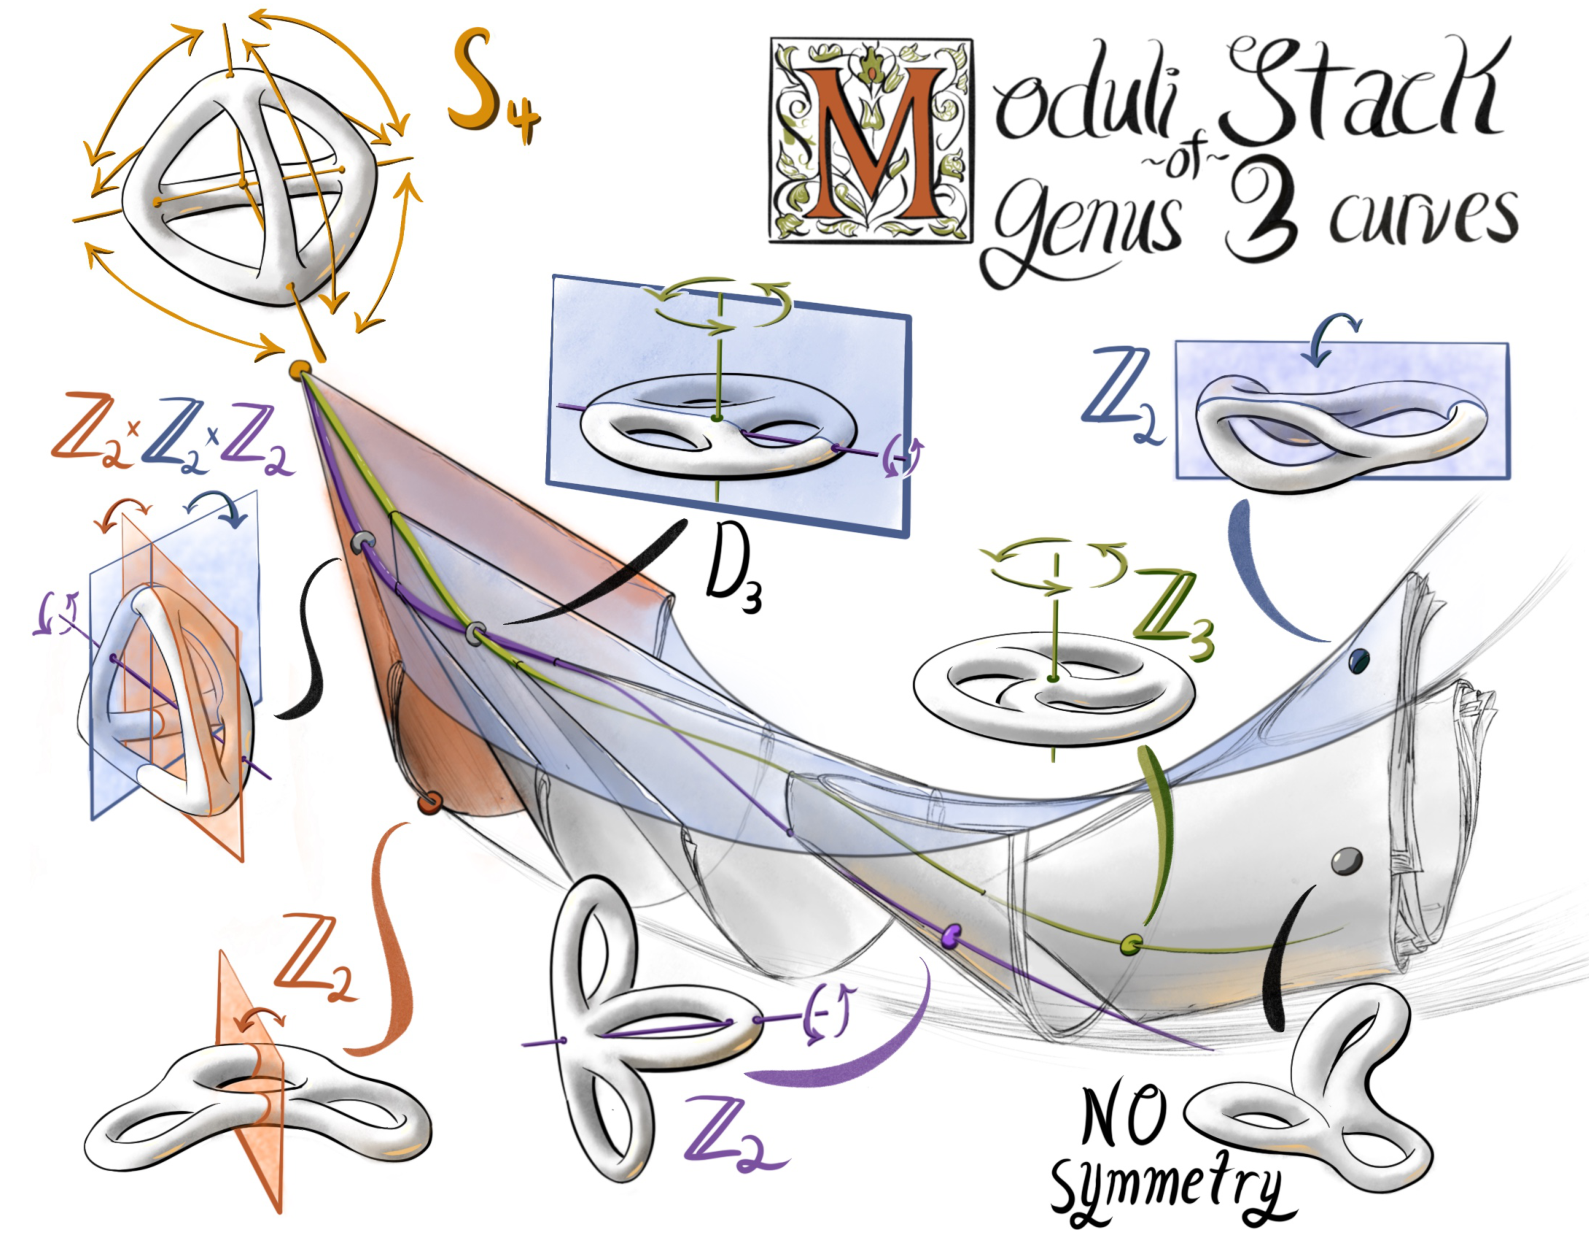
\includegraphics[width=.72\textwidth]{figures/fig-1.3.27.png}};
\begin{scope}[x={(art.south east)},y={(art.north west)}]
\fill[white] (.47,.755) rectangle (1,1);
\node[font=\small,align=center] at (.735,.89) {亏格为 $3$ 的曲线的模叠};
\fill[white] (.676,.085) rectangle (.739,.151);
\fill[white] (.655,.015) rectangle (.817,.079);
\node[font=\scriptsize] at (.73,.045) {无对称性};
\end{scope}
\end{tikzpicture}
\caption{$\mathcal M_3$ 的万有族示意图, 着重描绘具有非平凡对称群的 Riemann 曲面.}\label{src:1.3.27}
\end{figure}
\begin{example}\label{src:1.3.28}
射影空间的模函子 (例~\bookref{1.3.16}) 的万有族, 是 $\mathbb P^n$ 上的线丛 $\mathcal O(1)$, 连同截面
\[
x_0,\ldots,x_n\in\Gamma(\mathbb P^n,\mathcal O(1)).
\]
\end{example}
\begin{example}[代数拓扑中的分类空间]\label{src:1.3.29}
令 $G$ 为拓扑群, $\mathsf{Top}^{\mathrm{para}}$ 为仿紧拓扑空间组成的范畴, 其中态射定义到同伦等价. 代数拓扑中的一个定理断言, 函子
\[
\mathsf{Top}^{\mathrm{para}}\longrightarrow\Sets,\qquad
S\longmapsto\{\text{主 }G\text{-丛 }P\to S\}/(\text{同构})
\]
可由一个拓扑空间表出, 我们将它记作 $BG$, 并称为\newterm{分类空间}{classifying space}. 万有族通常记作 $EG\to BG$. 例如, 分类空间 $B\mathbb C^*$ 是无穷维流形 $\mathbb{CP}^{\infty}$. 然而, 在代数几何中, \newterm{分类叠}{classifying stack} $B\mathbb G_{m,\mathbb C}$ 是维数为 $-1$ 的代数叠.
\end{example}

\subsection{不可表模函子的例子}\label{src:1.3.5-subsection}
若 $F:\Sch/\mathbb C\to\Sets$ 为模函子, 那么具有非平凡自同构的对象 $E\in F(\mathbb C)$ 可能阻止函子 $F$ 的可表性. 原因是, 我们可以利用这个自同构粘合平凡族, 构造概形 $S$ 上的非平凡族 $\mathcal E$, 使每个纤维 $\mathcal E_s$(即 $\mathcal E$ 沿 $\operatorname{Spec}\mathbb C\to S$ 的拉回)都同构于 $E$.
\begin{proposition}\label{src:1.3.30}
令 $F:\Sch/\mathbb C\to\Sets$ 为模函子. 如果存在簇 $S$ 上的对象族 $\mathcal E\in F(S)$, 满足
\begin{enumerate}[(a)]
\item 对 $s\in S(\mathbb C)$, 纤维 $\mathcal E_s$ 彼此同构; 以及
\item 族 $\mathcal E$ 非平凡, 即它不等于任何对象 $E\in F(\mathbb C)$ 沿结构映射 $S\to\operatorname{Spec}\mathbb C$ 的拉回, 
\end{enumerate}
那么 $F$ 不可表.
\end{proposition}
\begin{proof}
反设 $F$ 可由概形 $X$ 表出. 由条件 (a), 限制 $E:=\mathcal E_s$ 与 $s\in S(\mathbb C)$ 无关, 并确定唯一的点 $x\in X(\mathbb C)$. 由于 $S$ 约化, 映射 $S\to X$ 分解为 $S\to\operatorname{Spec}\mathbb C\xrightarrow{x}X$. 这意味着族 $\mathcal E$ 为沿常值映射 $S\to\operatorname{Spec}\mathbb C\xrightarrow{x}X$ 的拉回, 即 $\mathcal E$ 为平凡族, 与条件 (b) 矛盾.
\end{proof}
\begin{exercise}[简单]\label{src:1.3.31}
证明将概形 $S$ 送到 $S$ 上的向量丛同构类的集合的模函子 $F:\Sch/\mathbb C\to\Sets$ 不可表.
\end{exercise}
\begin{example}[椭圆曲线的模]\label{src:1.3.32}
一条\textit{椭圆曲线}是一个二元组 $(E,p)$, 其中 $E$ 为亏格 $1$ 的光滑, 连通射影曲线, $p\in E(\mathbb C)$. 概形 $S$ 上的\textit{椭圆曲线族}是一个二元组 $(\mathcal E\to S,\sigma)$, 其中 $\mathcal E\to S$ 是带有截面 $\sigma:S\to\mathcal E$ 的光滑固有态射, 使对每个 $s\in S$, 纤维 $(\mathcal E_s,\sigma(s))$ 为剩余域 $\kappa(s)$ 上的椭圆曲线. 椭圆曲线的模函子为
\[
\begin{aligned}
F_{M_{1,1}}:&\ \Sch\longrightarrow\Sets,\\
&S\longmapsto\{\text{椭圆曲线族 }(\mathcal E\to S,\sigma)\}/\sim,
\end{aligned}
\]
其中, $(\mathcal E\to S,\sigma)\sim(\mathcal E'\to S,\sigma')$ 是指存在与截面相容的 $S$-同构 $\alpha:\mathcal E\to\mathcal E'$(即 $\sigma'=\alpha\circ\sigma$).
\end{example}
\begin{exercise}[适于练习]\label{src:1.3.33}
考虑在 $\mathbb A^1\setminus0$(坐标为 $t$)上由下图定义的椭圆曲线族: 
\[
\begin{tikzcd}[column sep=large]
\mathcal E:=V(y^2z-x^3+tz^3)\arrow[r,hook]\arrow[d] &
(\mathbb A^1\setminus0)\times\mathbb P^2\\
\mathbb A^1\setminus0 &
\end{tikzcd}
\]
截面 $\sigma:\mathbb A^1\setminus0\to\mathcal E$ 由 $t\mapsto[0,1,0]$ 给出. 证明 $(\mathcal E\to\mathbb A^1\setminus0,\sigma)$ 满足命题~\bookref{1.3.30}~中的 (a) 和 (b), 并推得 $F_{M_{1,1}}$ 不可表.
\end{exercise}
\begin{example}[光滑曲线的模函子]\label{src:1.3.34}
令 $C$ 为一条具有非平凡自同构 $\alpha\in\operatorname{Aut}(C)$ 的曲线, $N$ 为结点三次曲线, 可以将其理解为把 $\mathbb P^1$ 上的点 $0$ 和 $\infty$ 粘合而成的曲线. 取平凡族 $\pi:C\times\mathbb P^1\to\mathbb P^1$, 通过自同构 $\alpha$ 将纤维 $\pi^{-1}(0)$ 与 $\pi^{-1}(\infty)$ 粘合, 就能构造一个族 $\mathcal C\to N$. 要证明光滑曲线的模函子 $\Sch/\mathbb C\to\Sets$ 不可表, 只须证明 $\mathcal C\to N$ 非平凡.
\end{example}
\begin{figure}[htbp]
\centering
\begin{tikzpicture}
\node[anchor=south west,inner sep=0] (art) at (0,0) {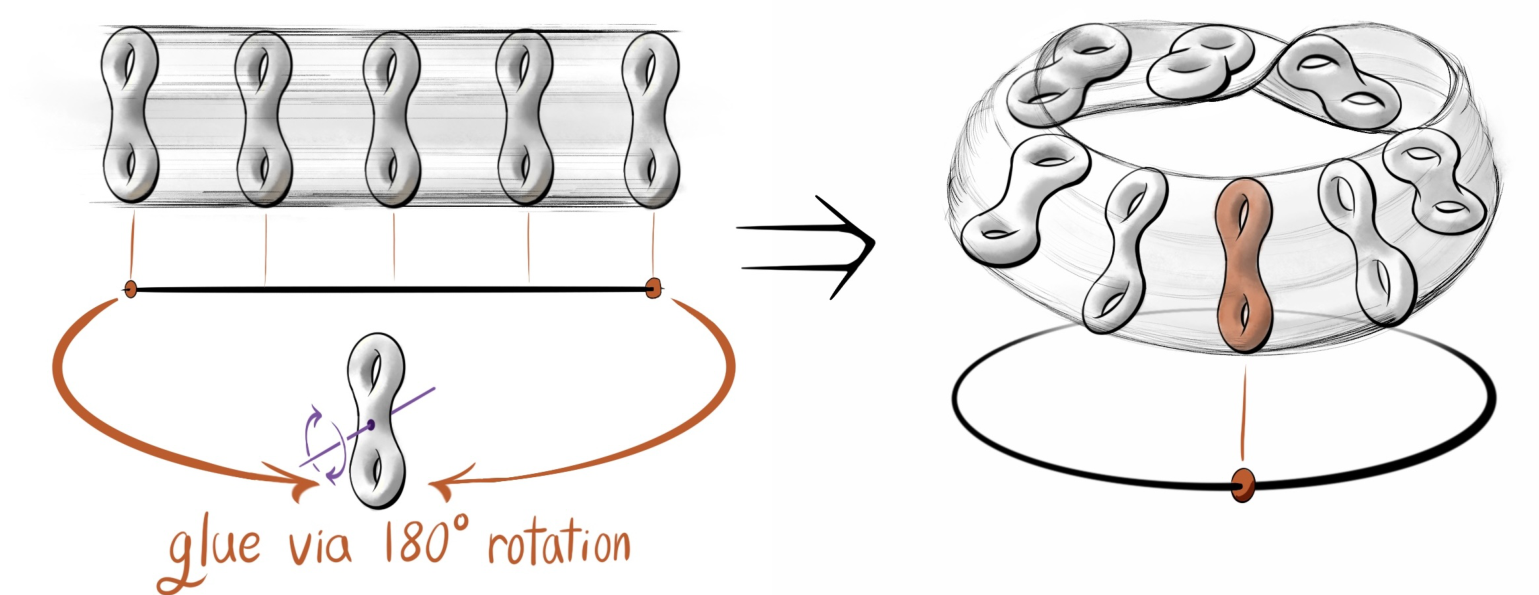
\includegraphics[width=.72\textwidth]{figures/fig-1.3.35.png}};
\begin{scope}[x={(art.south east)},y={(art.north west)}]
\fill[white] (.07,0) rectangle (.44,.15);
\node[font=\scriptsize] at (.26,.06) {通过 $180^\circ$ 旋转粘合};
\end{scope}
\end{tikzpicture}
\caption{通过非平凡自同构粘合平凡族, 得到一个由 Riemann 曲面组成的 Möbius 带.}\label{src:1.3.35}
\end{figure}
\begin{exercise}[补充细节]\label{src:1.3.36}
证明 $\mathcal C\to N$ 为非平凡族.
\end{exercise}
\begin{exercise}[适于练习]\label{src:1.3.37}
证明曲线 $C$ 上的向量丛的模函子不可表.
\end{exercise}

\subsection{概形是大 Zariski 拓扑中的层}\label{src:1.3.6-subsection}
若 $F:\Sch\to\Sets$ 可由概形 $X$ 表出, 则 $F$ 必为\newterm{大 Zariski 拓扑}{big Zariski topology}中的层. 也就是说, 对每个概形 $S$, 在 $S$ 的 Zariski 拓扑上, 将开子集 $U\subseteq S$ 送到集合 $F(U)$ 所定义的预层, 是 $S$ 的 Zariski 拓扑上的层. 这只是对``到固定概形 $X$ 的态射可以唯一粘合''的另一种表述. 因此, 不满足层条件便构成给定模函子 $F$ 可表性的另一种障碍.
\begin{exercise}[适于练习]\label{src:1.3.38}
\begin{enumerate}[(a)]
\item 证明下列朴素的 Grassmann 函子不可表: 
\[
F:\Sch\longrightarrow\Sets,\qquad
S\longmapsto\{q:\mathcal O_S^n\twoheadrightarrow\mathcal O_S^k\text{ 的商}\}/\sim.
\]
\item 在 $\mathbb G_m$ 对 $\mathbb A^{n+1}\setminus0$ 的通常数乘作用下, 证明函子 $S\mapsto(\mathbb A^{n+1}\setminus0)(S)/\mathbb G_m(S)$ 不是层.
\end{enumerate}
\end{exercise}
非平凡自同构的存在, 常常意味着给定的模函子不是大 Zariski 拓扑中的层.
\begin{example}\label{src:1.3.39}
考虑例~\bookref{1.3.8}~中的光滑曲线的模函子 $F_{M_g}$. 令 $\{S_i\}$ 为概形 $S$ 的 Zariski 开覆盖, 假设 $\mathcal C_i\to S_i$ 为光滑曲线族, 并在交集 $S_{ij}:=S_i\cap S_j$ 上有同构 $\alpha_{ij}:\mathcal C_i|_{S_{ij}}\xrightarrow{\sim}\mathcal C_j|_{S_{ij}}$. 要求 $F_{M_g}$ 为层(当限制到 $S$ 的 Zariski 拓扑时), 意味着这些族 $\mathcal C_i\to S_i$ 可以唯一粘合成一个曲线族 $\mathcal C\to S$. 然而, 我们并未要求同构 $\alpha_i$ 在三重交集上相容(即 $\alpha_{ij}|_{S_{ijk}}\circ\alpha_{jk}|_{S_{ijk}}=\alpha_{ik}|_{S_{ijk}}$), 而这却是粘合概形所必需的~\cite[习题 II.2.12]{Har77}. 因此, $F_{M_g}$ 不是层.
\end{example}
\begin{exercise}\label{src:1.3.40}
通过明确给出一个概形 $S$, 一个开覆盖 $\{S_i\}$, 以及无法粘合为 $S$ 上的族的 $S_i$ 上的曲线族, 证明光滑曲线和椭圆曲线的模函子都不是层.
\end{exercise}

\subsection{函子的运用}\label{src:1.3.7-subsection}
反变函子 $F:\Sch\to\Sets$ 组成范畴 $\operatorname{Fun}(\Sch,\Sets)$, 其中态射为自然变换. 这个范畴具有纤维积: 给定态射 $\alpha:F\to G$ 和 $\beta:G'\to G$, 定义
\[
\begin{aligned}
F\times_G G':&\ \Sch\longrightarrow\Sets,\\
&S\longmapsto
\{(a,b)\in F(S)\times G'(S)\mid\alpha_S(a)=\beta_S(b)\in G(S)\}.
\end{aligned}
\]
\begin{exercise}[简单]\label{src:1.3.41}
证明 $F\times_G G'$ 满足 $\operatorname{Fun}(\Sch,\Sets)$ 中纤维积的万有性质.
\end{exercise}
\begin{definition}\label{src:1.3.42}
\begin{enumerate}[(1)]
\item 称反变函子之间的态射 $F\to G$ \newterm{可由概形表出}{representable by schemes}, 是指对来自概形 $S$ 的每个映射 $S\to G$, 纤维积 $F\times_G S$ 都可由概形表出.
\item 称态射 $F\to G$ 为\newterm{开浸入}{open immersion}, 或称子函子 $F\subseteq G$ 为\textit{开的}, 是指对来自概形 $S$ 的每个态射 $S\to G$, $F\times_G S$ 都可由 $S$ 的一个开子概形表出.
\item 称 $F$ 的一组开子函子 $\{F_i\}$ 为 \newterm{Zariski 开覆盖}{Zariski open cover}, 是指对来自概形 $S$ 的每个态射 $S\to F$, $\{F_i\times_F S\}$ 都是 $S$ 的 Zariski 开覆盖(特别地, 每个 $F_i$ 都是 $F$ 的开子函子).
\end{enumerate}
\end{definition}
这些定义给出了检验给定函子 $F$ 是否可由概形表出的办法: 找出一个 Zariski 开覆盖 $\{F_i\}$, 使每个 $F_i$ 都可表.
\begin{exercise}[简单]\label{src:1.3.43}
证明: 若 $F$, $G$ 及各 $F_i$ 都是大 Zariski 拓扑中的层, 那么定义~\bookref{1.3.42}~的各个条件只须对来自仿射概形 $S$ 的映射检验.
\end{exercise}
\begin{exercise}[适于练习]\label{src:1.3.44}
\begin{enumerate}[(a)]
\item 令 $F:\Sch\to\Sets$ 为大 Zariski 拓扑中的层, $\{F_i\}$ 为 $F$ 的 Zariski 开覆盖. 证明: 若每个 $F_i$ 都可由概形表出, 则 $F$ 也可由概形表出.
\item 证明: $F$ 的一组开子函子 $\{F_i\}$ 为 Zariski 开覆盖, 当且仅当对每个代数闭域 $\Bbbk$, 映射 $\coprod_i F_i(\Bbbk)\to F(\Bbbk)$ 为满射.
\item 给定概形态射 $X\to Y$ 和 $Y'\to Y$, 通过给出 $X\times_Y Y'$ 的一个 Zariski 开覆盖 $\{F_i\}$, 使每个 $F_i$ 都可由仿射概形表出, 重新证明概形范畴中纤维积 $X\times_Y Y'$ 的存在性.
\end{enumerate}
\end{exercise}
\begin{exercise}[概形的函子定义]\label{src:1.3.45}
证明概形也可以等价地定义为仿射概形范畴上的反变函子 $F:\mathsf{AffSch}\to\Sets$(或环范畴上的协变函子), 具体如下. 令 $\mathcal C$ 为反变函子范畴 $\operatorname{Fun}(\mathsf{AffSch},\Sets)$ 的一个满子范畴.

推广定义~\bookref{1.3.15}~和~\bookref{1.3.42}, 若存在对象 $X\in\mathcal C$, 使对每个 $S\in\mathsf{AffSch}$ 都有具有函子性的等价 $F(S)=\operatorname{Mor}(S,X)$, 则称函子 $F:\mathsf{AffSch}\to\Sets$ \textit{在 $\mathcal C$ 中可表}. 称从 $\mathsf{AffSch}$ 到 $\Sets$ 的函子之间的映射 $F\to G$ \textit{可由 $\mathcal C$ 中的开浸入表出}, 是指对每个态射 $\operatorname{Spec}B\to G$, 纤维积 $F\times_G\operatorname{Spec}B$ 都可由对象 $X\in\mathcal C$ 表出, 且 $X$ 为 $\operatorname{Spec}B$ 的开子概形. 最后, 称 $F$ 的一组子函子 $\{F_i\}$ 为 \textit{Zariski 开 $\mathcal C$-覆盖}, 是指每个 $F_i\to F$ 都可由 $\mathcal C$ 中的开浸入表出, 且对每个代数闭域 $\Bbbk$, 映射 $\coprod_i F_i(\Bbbk)\to F(\Bbbk)$ 为满射.
\begin{enumerate}[(a)]
\item 取 $\mathcal C=\mathsf{AffSch}$, 证明具有仿射对角态射的概形, 可等价地定义为一个函子 $F:\mathsf{AffSch}\to\Sets$, 满足: 存在 $F$ 的一个 Zariski 开 $\mathcal C$-覆盖 $\{F_i\}$, 且每个 $F_i$ 都在 $\mathcal C$ 中可表.
\item 取 $\mathcal C$ 为具有仿射对角态射的概形组成的范畴, 证明概形可等价地定义为一个函子 $F:\mathsf{AffSch}\to\Sets$, 满足: 存在一个 Zariski 开 $\mathcal C$-覆盖 $\{F_i\}$, 且每个 $F_i$ 都在 $\mathcal C$ 中可表.
\item 或者, 证明概形可定义为拟仿射概形范畴上的某个适当的反变函子.
\end{enumerate}
\end{exercise}
将上面习题中的 Zariski 开集换成平展态射, 就得到代数空间的定义(定义~\bookref{4.1.2}).
\begin{exercise}[困难]\label{src:1.3.46}
令 $X\to Y$ 为概形态射, 其中 $X$ 和 $Y$ 都在概形 $S$ 上固有. 若 $X$ 在 $S$ 上平坦, 证明参数化概形映射 $T\to S$, 使 $X_T\xrightarrow{\sim}Y_T$ 为同构的子函子 $F\subseteq\operatorname{Mor}(-,S)$, 可由一个开子函子表出.

\textit{提示: }若 $s\in S$ 为一个使 $X_s\to Y_s$ 为同构的点, 利用纤维平坦性判别法(\bookref{A.2.10})证明 $X\to Y$ 在 $s$ 上平坦. 然后归约到 $X\to Y$ 为有限平展态射的情形.
\end{exercise}

% Source printed pp. 28-31, entire Section 1.4.
\section{模群胚}\label{src:1.4}
\begin{epigraph}
我目前得出的实际结论是: 每当按照我的判别准则, 尽管具有良好的平坦性, 固有性以及可能的非奇异性假设, 却仍不存在用来分类某些结构(非奇异完备簇, 向量丛等)的(整体或无穷小)变化的模簇(更准确地说, 模概形)时, 原因仅仅在于这些结构具有自同构, 使下降技术无法奏效.
\epigraphauthor{Alexander Grothendieck, 致 Serre 的信, $1959$ 年~\cite[第 94 页]{CS01}}
\end{epigraph}
现在我们改变观点: 我们不只指定两个对象\textit{何时}被等同, 还要指定它们\textit{如何}被等同!

模空间最令人期待的性质之一, 是存在万有族(见 \S\bookref{1.3.4-subsection}); 而自同构的存在阻碍了万有族的存在(见 \S\bookref{1.3.5-subsection}). 在描述中纳入自同构, 将使我们能够克服这个问题. 定义一个模群胚, 需要明确: 
\begin{enumerate}[(1)]
\item 对象; 以及
\item 任意两个对象之间的等同所组成的集合(可能为空).
\end{enumerate}
不久, 我们将把上一节的函子观点与这一群胚观点结合起来, 定义模叠.

\subsection{群胚}\label{src:1.4.1-subsection}
用来编码对象及其等同的一种便利的数学结构, 就是群胚.
\begin{definition}\label{src:1.4.1}
\newterm{群胚}{groupoid}是一个范畴 $\mathcal C$, 其中每个态射都是同构.
\end{definition}
两个群胚 $\mathcal C_1$ 和 $\mathcal C_2$ \textit{等价}, 是指存在范畴等价 $F:\mathcal C_1\xrightarrow{\sim}\mathcal C_2$, 即存在函子 $G:\mathcal C_2\to\mathcal C_1$, 使 $F\circ G$ 和 $G\circ F$ 都同构于恒等函子; 等价地, $F$ 完全忠实且本质满.
\begin{example}[集合是群胚]\label{src:1.4.2}
若 $\Sigma$ 为集合, 则范畴 $\mathcal C_\Sigma$ 为群胚, 其对象是 $\Sigma$ 的元素, 而态射只有恒等态射. 若存在范畴等价 $\mathcal C\to\mathcal C_\Sigma$, 则称群胚 $\mathcal C$ \textit{等价于集合 $\Sigma$}.
\end{example}
\begin{example}[分类群胚]\label{src:1.4.3}
若 $G$ 为群, $G$ 的\newterm{分类群胚}{classifying groupoid} $BG$ 定义为只有一个对象 $\star$ 的范畴, 满足 $\operatorname{Aut}(\star)=\operatorname{Mor}(\star,\star)=G$.
\end{example}
\begin{example}\label{src:1.4.4}
由有限集组成, 以双射为态射的范畴 $\mathsf{FB}$ 是群胚. $\mathsf{FB}$ 的同构类与 $\mathbb N$ 一一对应.

而 $\operatorname{Aut}(\{1,\ldots,n\})=S_n$ 是置换群.
\end{example}
\begin{example}[射影空间]\label{src:1.4.5}
射影空间等同于过原点的直线 $L\subset\mathbb A^{n+1}$ 的模群胚, 其中态射只有恒等映射. 也可以将对象取为非零线性映射 $x=(x_0,\ldots,x_n):\mathbb C\to\mathbb C^{n+1}$, 且存在唯一态射 $x\to x'$ 当且仅当 $\operatorname{im}(x)=\operatorname{im}(x')\subseteq\mathbb C^{n+1}$(即存在 $\lambda\in\mathbb C^*$, 使 $x'=\lambda x$).
\end{example}

\subsection{轨道的模群胚}\label{src:1.4.2-subsection}
\begin{example}[轨道的模群胚]\label{src:1.4.6}
给定群 $G$ 在集合 $X$ 上的作用, 定义\textit{轨道的模群胚} $[X/G]$\footnote{我们用方括号区分群胚商 $[X/G]$ 与集合商 $X/G$. 后面, 当 $G$ 为代数群, $X$ 为概形时, $[X/G]$ 将表示商叠(它总是存在), 而 $X/G$ 将表示商空间(如果存在).}, 其对象为所有元素 $x\in X$, 并规定 $\operatorname{Mor}(x,x')=\{g\in G\mid x'=gx\}$.
\end{example}
\begin{figure}[htbp]
\centering\begin{tikzpicture}[x=1cm,y=1cm,>=Stealth,font=\small]
\begin{scope}
\draw (-1.2,1.4)..controls (.2,1.4) and (.2,.6)..(1.2,.6);
\draw (-1.2,.6)..controls (.2,.6) and (.2,1.4)..(1.2,1.4);
\node[right] at (1.35,1) {$\mathbb A^1$};
\draw[->] (0,.55)--(0,.13);
\draw (-1.2,0)--(1.2,0);
\fill (0,0) circle (1.8pt);
\node[below,blue] at (0,0) {$\mathbb Z/2$};
\node[right] at (1.35,0) {$[\mathbb A^1/(\mathbb Z/2)]$};
\end{scope}
\begin{scope}[xshift=7cm]
\draw (-1.2,1)--(1.2,1);
\fill (0,1) circle (1.8pt);\node[above] at (0,1) {$0$};
\node[right] at (1.35,1) {$\mathbb A^1$};
\draw[->] (0,.8)--(0,.23);
\fill (0,0) circle (1.8pt);
\shade[ball color=gray] (.7,0) circle (.10);
\draw[gray,densely dotted] (.6,0)--(.1,0);
\node[below,blue] at (0,0) {$\mathbb G_m$};
\node[below,blue] at (.7,0) {$\{1\}$};
\node[right] at (1.35,0) {$[\mathbb A^1/\mathbb G_m]$};
\end{scope}
\end{tikzpicture}

\caption{$\mathbb Z/2=\{\pm1\}$ 和 $\mathbb G_m$ 在 $\mathbb C$ 上的 $\mathbb A^1$ 上的数乘作用, 自同构群以蓝色列出. 注意, $[\mathbb A^1/\mathbb G_m]$ 有两个对象同构类, 即 $0$ 和 $1$, 对应于两个轨道, 即 $0$ 和 $\mathbb A^1\setminus0$. 若赋予集合 $\mathbb A^1/\mathbb G_m$ 商拓扑, 则 $0\in\overline{\{1\}}$.}\label{src:1.4.7}
\end{figure}
\begin{exercise}[简单]\label{src:1.4.8}
证明例~\bookref{1.4.6}~中轨道的模群胚 $[X/G]$ 等价于一个集合, 当且仅当 $G$ 在 $X$ 上的作用自由.
\end{exercise}
\begin{example}\label{src:1.4.9}
考虑具有两个对象 $x_1$ 和 $x_2$ 的范畴 $\mathcal C$, 对 $i,j=1,2$ 有 $\operatorname{Mor}(x_i,x_j)=\{\pm1\}$, 态射的复合由乘法给出. 那么 $\mathcal C$ 等价于 $B(\mathbb Z/2)$.
\end{example}
\begin{figure}[htbp]
\centering\begin{tikzpicture}[>=Stealth,font=\small]
\node[circle,fill,inner sep=3pt,label=below:$x_1$] (a) at (0,0) {};
\node[circle,fill,inner sep=3pt,label=below:$x_2$] (b) at (3,0) {};
\node[circle,fill,inner sep=3pt,label=below:$x$] (c) at (7.1,0) {};
\foreach \v in {a,b,c} {
\path[->] (\v) edge[out=150,in=30,looseness=16] node[above] {$1$} (\v);
\path[->] (\v) edge[out=135,in=45,looseness=10] node[below,pos=.5] {$-1$} (\v);
}
\path[->] (a) edge[bend left=18] node[above] {$1$} (b);
\path[->] (a) edge[bend left=32] node[above] {$-1$} (b);
\path[->] (b) edge[bend left=18] node[below] {$1$} (a);
\path[->] (b) edge[bend left=32] node[below] {$-1$} (a);
\draw[->] (4,.15)--(5.9,.15) node[midway,above] {$\sim$};
\node at (4.95,-.35) {$x_i\longmapsto x$};
\end{tikzpicture}

\caption{群胚的一个等价.}\label{src:1.4.10}
\end{figure}
\begin{exercise}[简单]\label{src:1.4.11}
在例~\bookref{1.4.9}~中, 证明 $\mathcal C$ 与 $[(\mathbb Z/2)/(\mathbb Z/4)]$ 或 $[(\mathbb Z/2)/(\mathbb Z/2\times\mathbb Z/2)]$ 之间存在一个在对象上诱导双射的范畴等价, 其中作用由满射 $\mathbb Z/4\to\mathbb Z/2$ 或 $\mathbb Z/2\times\mathbb Z/2\to\mathbb Z/2$ 给出.
\end{exercise}
\begin{example}[射影空间作为商]\label{src:1.4.12}
射影空间的模群胚(例~\bookref{1.4.5})也可以描述为轨道的模群胚 $[(\mathbb A^{n+1}\setminus0)/\mathbb G_m]$. 还可以考虑商群胚 $[\mathbb A^{n+1}/\mathbb G_m]$, 它等价于如下群胚: 对象为(可能为零的)线性映射 $x=(x_0,\ldots,x_n):\mathbb C\to\mathbb C^{n+1}$, 且 $\operatorname{Mor}(x,x')=\{t\in\mathbb C^*\mid\text{对所有 }i\text{ 有 }x'_i=tx_i\}$. 由此, $\mathbb P^n$ 是 $[\mathbb A^{n+1}/\mathbb G_m]$ 的一个子群胚.
\end{example}
\begin{exercise}[简单, 适于练习]\label{src:1.4.13}
若群 $G$ 在集合 $X$ 上作用, $x\in X$ 为稳定子是 $G_x$ 的点, 证明存在完全忠实函子 $BG_x\to[X/G]$. 若作用传递, 证明该函子为等价.
\end{exercise}
按定义, 群胚的\textit{态射} $\mathcal C_1\to\mathcal C_2$ 是一个函子. 范畴 $\operatorname{Mor}(\mathcal C_1,\mathcal C_2)$ 的对象为函子, 态射为自然变换.
\begin{exercise}[简单]\label{src:1.4.14}
若 $\mathcal C_1$ 和 $\mathcal C_2$ 为群胚, 证明 $\operatorname{Mor}(\mathcal C_1,\mathcal C_2)$ 为群胚.
\end{exercise}
\begin{exercise}[中等, 适于练习]\label{src:1.4.15}
若 $H$ 和 $G$ 为群, 证明存在等价
\[
\operatorname{Mor}(BH,BG)=
\coprod_{\phi\in\operatorname{Hom}(H,G)/G} B\bigl(C^G(\operatorname{im}\phi)\bigr),
\]
其中, $\operatorname{Hom}(H,G)/G$ 表示同态 $H\to G$ 模去 $G$ 的共轭作用后的等价类, $C^G(\operatorname{im}\phi)$ 表示 $\operatorname{im}\phi$ 在 $G$ 中的中心化子.
\end{exercise}
\begin{exercise}\label{src:1.4.16}
给出群 $H$ 和 $G$ 分别在集合 $X$ 和 $Y$ 上作用的一个例子, 以及群胚映射 $[X/H]\to[Y/G]$, 使该映射不能由群同态 $\phi:H\to G$ 与一个 $\phi$-等变映射 $X\to Y$ 产生.
\end{exercise}

\subsection{模群胚的例子}\label{src:1.4.3-subsection}
\begin{example}[光滑曲线的模群胚]\label{src:1.4.17}
对象为 $\mathbb C$ 上亏格为 $g$ 的光滑, 连通射影曲线. 对两条曲线 $C,C'$, 态射集合定义为同构集合
\[
\operatorname{Mor}(C,C')=\{\text{同构 }\alpha:C\xrightarrow{\sim}C'\}.
\]
\end{example}
\begin{example}[曲线上向量丛的模群胚]\label{src:1.4.18}
对象为固定曲线 $C$ 上秩为 $r$, 次数为 $d$ 的向量丛 $E$, 态射为向量丛的同构.
\end{example}
\begin{example}[无标号三角形的模群胚]\label{src:1.4.19}
回到例~\bookref{1.2.12}~中相似关系下无标号三角形的模 $M^{\mathrm{unl}}$. 回忆我们已经引入了无标号三角形的族, 并证明了这个函子不可表(例~\bookref{1.3.6}).

定义相似关系下\textit{无标号三角形的模群胚}, 记作 $\mathcal M^{\mathrm{unl}}$(注意花体), 其中对象为无标号三角形, 态射为相似变换. 例如, 等腰三角形和等边三角形的自同构群分别为 $\mathbb Z/2$ 和 $S_3$. 我们可以画出与图~\bookref{1.2.14}~基本相同的图, 只是还要记录自同构.
\end{example}
\begin{figure}[htbp]
\centering\begin{tikzpicture}[scale=5.5]
\fill[gray!30] (0,1)--(.5,.5)--(2/3,2/3)--cycle;
\draw[->] (0,0)--(1.08,0) node[right] {$a$};
\draw[->] (0,0)--(0,1.1) node[above] {$b$};
\draw[densely dotted] (0,1)--(.5,.5);
\draw[blue!35,line width=2pt] (0,1)--(2/3,2/3)--(.5,.5);
\draw[magenta,thick,domain=0:{2-sqrt(2)},samples=100] plot (\x,{(2-2*\x)/(2-\x)});
\fill[green!75!black] (2/3,2/3) circle (.012);
\foreach \v/\t in {0.5/{1/2},0.6666667/{2/3}} {
\draw (\v,0)--(\v,-.02) node[below] {$\t$};
\draw (0,\v)--(-.02,\v) node[left] {$\t$};
}
\node[left] at (0,1) {$1$};
\node[font=\small,rotate=-45,fill=white,inner sep=1pt] at (.2,.75) {$a+b=c$};
\node[font=\small,rotate=-27,above] at (.25,.9) {$b=c$};
\node[font=\small,rotate=45,below] at (.59,.57) {$a=b$};
\node[blue,rotate=-27,above] at (.44,.82) {$\mathbb Z/2$};
\node[blue,rotate=45,below] at (.66,.58) {$\mathbb Z/2$};
\node[right,green!75!black] at (.69,.68) {$S_3$};
\draw[->,gray] (.93,.86)--(.68,.69);\node[right,font=\small] at (.8,.89) {等边};
\draw[->] (.16,.25)--(.43,{(2-2*.43)/(2-.43)});
\node[font=\small] at (.17,.18) {$a^2+b^2=c^2$};
\end{tikzpicture}

\caption{模群胚 $\mathcal M^{\mathrm{unl}}$ 的示意图, 标出了非平凡自同构群.}\label{src:1.4.20}
\end{figure}
存在从模群胚到模集合的函子
\[
\mathcal M^{\mathrm{unl}}\longrightarrow M^{\mathrm{unl}},
\]
它在对象的同构类上给出等价, 并将所有态射压缩为恒等态射. 这是粗模空间的第一个例子.
\begin{exercise}\label{src:1.4.21}
回忆~\eqref{src:1.2.6}~中相似关系下带标号三角形的模集合 $M^{\mathrm{lab}}$ 的描述, 证明 $S_3$ 在相似关系下带标号三角形的模集合 $M^{\mathrm{lab}}$ 上有自然作用, 并且存在群胚的等同 $\mathcal M^{\mathrm{unl}}\cong[M^{\mathrm{lab}}/S_3]$.
\end{exercise}
\begin{exercise}\label{src:1.4.22}
定义有向三角形的模群胚, 并研究它与带标号及无标号三角形的模群胚之间的关系.
\end{exercise}
关于三角形的模叠的更详细阐述, 见~\cite{Beh14}.

% Source printed pp. 32-35, entire Section 1.5.
\section{为何使用平展拓扑?}\label{src:1.5}
\begin{epigraph}
可以说, 从 Zariski 拓扑转到平展拓扑时, 对于一个有限常值系数群 $G$, 为了得到``正确的'' $H^1$, 我们已经``做了该做的事''...一个值得注意的事实是, 这也足以对任意挠系数群找到``正确的'' $H^i(X,G)$(至少当 $G$ 与 $X$ 的剩余特征互素时). 这将在本讨论班的后续部分证明.
\epigraphauthor{Alexander Grothendieck~\cite[VII.2.1]{SGA4}}
\end{epigraph}
下一节将通过结合模函子与群胚来引入模叠: 需要指定每个概形 $S$ 上的对象族, 以及它们之间的等同和拉回. 为使这些数据定义一个\textit{叠}, 我们将要求对象及其态射在\textit{平展}拓扑中能够粘合!据说, Grothendieck 创造``étale''一词, 是因为平展态射使他联想到满月下涨潮时平静的海面, 正如 Victor Hugo 在``海上劳工''中写道: ``海面平静, 但退潮已开始显现.''

为何 Zariski 拓扑不足以满足我们的需要?简短的回答是: Zariski 开子集不够多, 而平展态射可以很好地替代解析开子集.

\subsection{平展态射究竟是什么?}\label{src:1.5.1-subsection}
有时我会感到困惑: 一个学生竟会被平展态射吓住, 尤其是当她已经掌握了概念上更困难的固有性, 平坦性等概念时. 一个原因可能是, 这一定义埋藏在~\cite[习题 III.10.3--6]{Har77}~中, 那里并未突出它的重要性.
% The supplied draft has no numbered object 1.5.1. It prints 1.5.2
% both beside the illustration and in its caption; retain both occurrences.
\setcounter{theorem}{1}
\begin{figure}[htbp]
\centering
\begin{minipage}[c]{.26\textwidth}
\centering
\begin{tikzpicture}[x=.75cm,y=.75cm,baseline=(current bounding box.center)]
\draw (-1.5,2)..controls (.4,2) and (-.4,1)..(1.5,1);
\draw (-1.5,1)..controls (.4,1) and (-.4,2)..(1.5,2);
\filldraw[fill=white] (0,1.5) circle (1.5pt);
\draw[->] (0,.85)--(0,.15);
\draw (-1.5,0)--(1.5,0);
\filldraw[fill=white] (0,0) circle (1.5pt);
\end{tikzpicture}
\end{minipage}\hfill
\begin{minipage}[c]{.16\textwidth}
\centering
$\begin{tikzcd}[row sep=large,column sep=small]
\mathbb A^1\arrow[d] & x\arrow[d,mapsto]\\
\mathbb A^1 & x^2
\end{tikzcd}$
\end{minipage}\hfill
\begin{minipage}[c]{.30\textwidth}
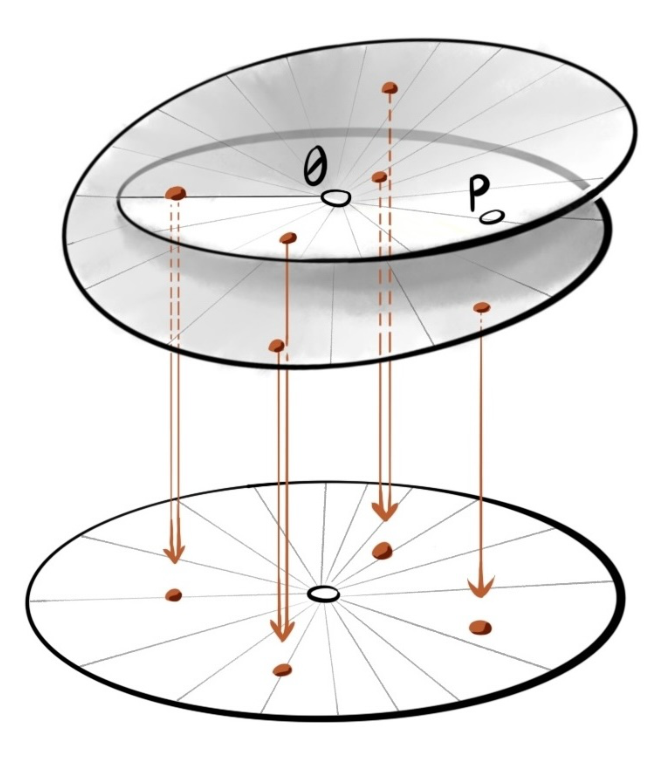
\includegraphics[width=\linewidth]{figures/fig-1.5.2-complex.png}
\end{minipage}\hfill
\begin{minipage}[c]{.12\textwidth}
\raggedleft(\ref{src:1.5.2})
\end{minipage}
\caption{$\mathbb A^1\setminus0$ 的平展二重覆盖. 左图画在 $\mathbb R$ 上(不过, 我们仍将负数的两个平方根画了出来), 右图画在 $\mathbb C$ 上.}\label{src:1.5.2}
\end{figure}
心中应有的几何图像是一个覆盖空间. 对 $\mathbb C$ 上有限型概形之间的态射 $f:X\to Y$, 平展性可以用以下几种方式表述: 
\begin{itemize}
\item $f$ 光滑且相对维数为 $0$(即 $f$ 平坦, 且所有纤维都光滑, 维数为 $0$); 
\item $f$ 平坦且非分歧(即对所有 $y\in Y(\mathbb C)$, 概形论纤维 $X_y$ 同构于点的不交并 $\coprod_i\operatorname{Spec}\mathbb C$); 
\item $f$ 平坦且 $\Omega_{X/Y}=0$; 
\item 对所有 $x\in X(\mathbb C)$, 在完备化上诱导的映射 $\widehat{\mathcal O}_{Y,f(x)}\to\widehat{\mathcal O}_{X,x}$ 为同构; 以及
\item 若还假设 $X$ 和 $Y$ 光滑, 则对所有 $x\in X(\mathbb C)$, 在切空间上诱导的映射 $T_{X,x}\to T_{Y,f(x)}$ 为同构.
\end{itemize}
若存在 $x\in X$ 的开邻域 $U$, 使 $f|_U$ 平展, 则称 $f$ \textit{在 $x$ 处平展}. 更多背景见 \S\bookref{A.3}. 这些刻画都彼此等价, 但绝不应认为你理当看出这一点: 有些证明相当复杂. 不过, 若暂且接受这些等价性, 那么只须很少的努力, 就不但能理解这一概念, 还能掌握它的运用.
\begin{exercise}[适于练习]\label{src:1.5.3}
证明 $f:\mathbb A^1\to\mathbb A^1$, $x\mapsto x^2$ 在 $\mathbb A^1\setminus0$ 上平展, 但在原点处不平展. 尝试尽可能多地使用上述刻画来证明.
\end{exercise}

\subsection{在平展拓扑中能看到什么?}\label{src:1.5.2-subsection}
使用平展拓扑, 就像给你的代数几何眼镜加上一副放大镜, 使你能看清那些通过微分几何眼镜早已能观察到的精细结构.
\begin{example}[结点的可约性]\label{src:1.5.4}
考虑平面中由 $y^2=x^2(x-1)$ 定义的平面结点三次曲线 $C$. 结点 $p=(0,0)$ 有一个可约的解析开邻域, 却没有这样的 Zariski 开邻域. 然而, 取 $x-1$ 的``平方根'', 就得到一个可约的平展邻域. 更具体地, 定义
$C'=\operatorname{Spec}\mathbb C[x,y,t]_t/(y^2-x^3+x^2,t^2-x+1)$, 并考虑
\[
C'\longrightarrow C,\qquad(x,y,t)\longmapsto(x,y).
\]
由于 $y^2-x^3+x^2=(y-xt)(y+xt)$, 可见 $C'$ 可约. 下图说明了这一点, 此图也见于~\cite[习题 III.10.6]{Har77}.
\end{example}
\begin{figure}[htbp]
\centering
\begin{tikzpicture}
\node[anchor=south west,inner sep=0] (art) at (0,0) {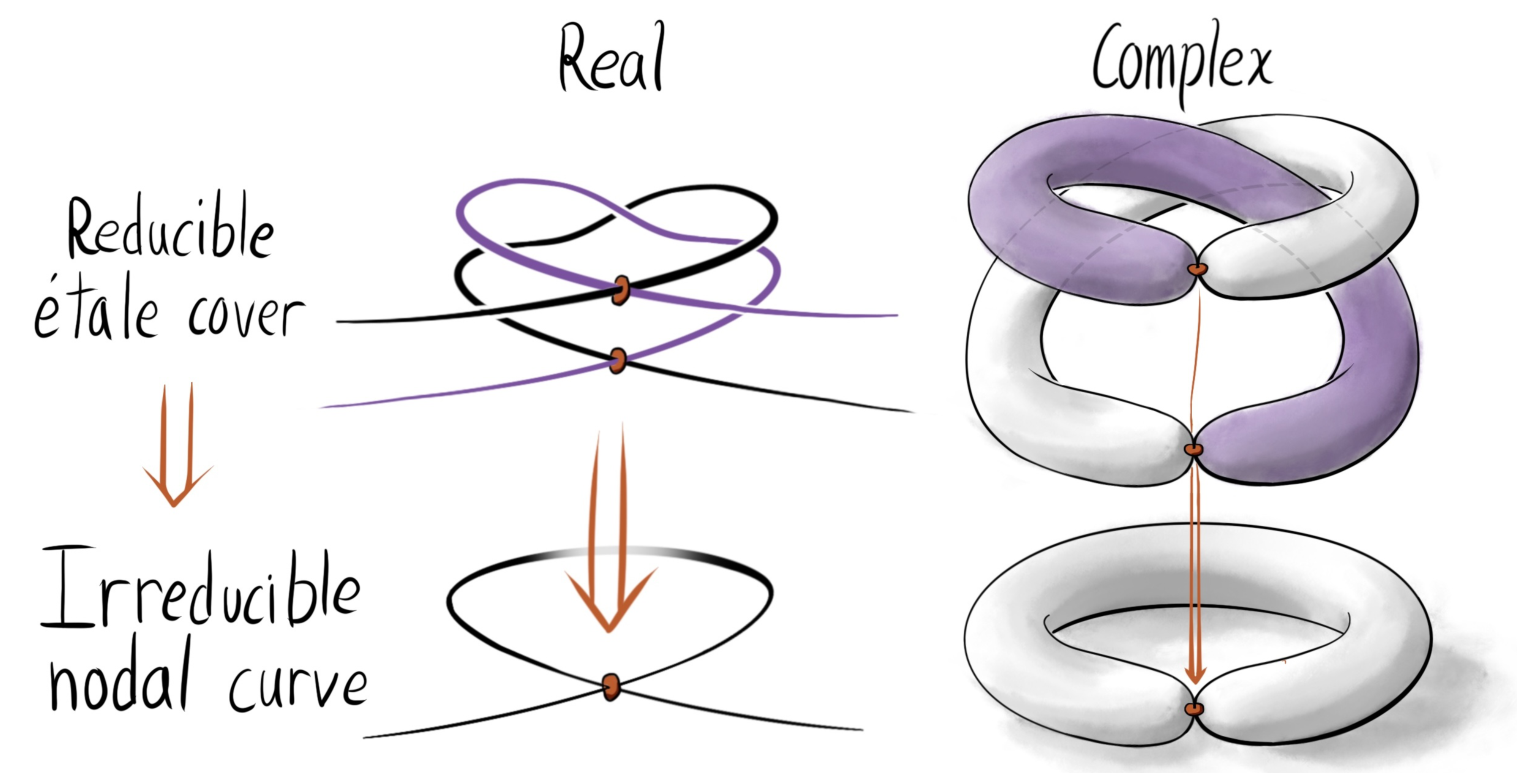
\includegraphics[width=.70\textwidth]{figures/fig-1.5.5.png}};
\begin{scope}[x={(art.south east)},y={(art.north west)}]
\fill[white] (.31,.88) rectangle (.44,1);
\node[font=\small] at (.375,.945) {实情形};
\fill[white] (.66,.85) rectangle (.86,1);
\node[font=\small] at (.76,.945) {复情形};
\fill[white] (.005,.535) rectangle (.215,.78);
\node[font=\scriptsize,align=center] at (.115,.67) {可约的\\平展覆盖};
\fill[white] (.012,.075) rectangle (.245,.31);
\node[font=\scriptsize,align=center] at (.13,.18) {不可约的\\结点曲线};
\end{scope}
\end{tikzpicture}
\caption{经过平展覆盖后, 结点三次曲线变得可约.}\label{src:1.5.5}
\end{figure}
\begin{example}[平展上同调]\label{src:1.5.6}
Zariski 拓扑中的层上同调可以推广到平展拓扑, 得到极为强大的\newterm{平展上同调}{étale cohomology}理论. 例如, 对 $\mathbb C$ 上亏格为 $g$ 的光滑射影曲线 $C$, 有限常值层 $\mathbb Z/n$ 的平展上同调 $H^1(C_{\text{ét}},\mathbb Z/n)$ 同构于 $(\mathbb Z/n)^{2g}$, 正如通常的上同调群一样; 而 Zariski 拓扑中的层上同调 $H^1(C,\mathbb Z/n)$ 为 $0$. 最后, 如果不提及平展上同调在证明 Weil 猜想方面的惊人应用, 那就有所疏漏了.
\end{example}
\begin{example}[平展基本群]\label{src:1.5.7}
你是否想过, Galois 理论中间域扩张与 Galois 群的子群之间的双射, 与代数拓扑中覆盖空间与基本群的子群之间的双射, 有某种相似之处?那么你并不孤单: Grothendieck 也考虑过这一点, 并发展出优美的\newterm{平展基本群}{étale fundamental group}理论, 将 Galois 群和基本群纳入同一框架.
\end{example}
\begin{example}[有限群自由作用的商]\label{src:1.5.8}
若有限群 $G$ 在射影簇 $X$ 上自由作用, 则商 $X/G$ 作为射影簇存在. 根本原因在于, 每个 $G$-轨道(事实上, 每个有限点集)都包含于一个仿射簇 $U$, 它是某个超曲面的补集. 于是, 所有 $G$-平移的交集 $V=\bigcap_g gU$ 是包含 $Gx$ 的 $G$-不变仿射开集, 且 $V/G=\operatorname{Spec}\Gamma(V,\mathcal O_V)^G$. 这些局部商粘合成整体商 $X/G$. 见推论~\bookref{5.2.13}~和习题~\bookref{5.2.14}.

然而, 若 $X$ 不是射影的, 则商未必作为概形存在. 与光滑固有但非射影簇的大多数现象一样, 可以用 Hironaka 的光滑固有三维簇的例子构造反例; 见~\cite[附录 B, 例 3.4.1]{Har77}. 存在一个光滑固有三维簇, 具有 $G=\mathbb Z/2$ 的自由作用, 且某个轨道 $Gx$ 不包含于任何 $G$-不变仿射开集. 这说明 $X/G$ 不可能作为概形存在: 事实上, 若它存在, 则 $x$ 在有限态射 $X\to X/G$ 下的像包含于某个仿射开集, 其逆像就会是 $X$ 中包含 $Gx$ 的仿射开子集. 细节见~\cite[例 1.3]{Knu71}~或~\cite[例 5.3.2]{Ols16}.

尽管如此, 对有限群 $G$ 在概形 $X$ 上的自由作用, 每个点 $x\in X$ 都有一个 $G$-等变平展邻域 $U_x\to X$, 其中 $U_x$ 为仿射概形. 商 $U_x/G$ 可以在平展拓扑中粘合, 将 $X/G$ 构造成代数空间(推论~\bookref{4.1.14}). 结论是, 我们总能取有限群自由作用的商. 鉴于群作用在代数几何中无处不在, 这一性质非常可贵, 但代价是必须将范畴从概形扩大到代数空间.
\end{example}
\begin{example}[Artin 逼近]\label{src:1.5.9}
Artin 逼近(\bookref{B.5.18})是 Michael Artin 的一个强大而极深刻的结果, 它意味着局部环的完备化 $\widehat{\mathcal O}_{X,x}$ 所具有的大多数性质, 也在 $x$ 的某个平展邻域中成立. 例如, 由于结点奇点处局部环的完备化可约, Artin 逼近意味着存在一个可约的平展邻域.
\end{example}

\subsection{使用平展拓扑: 下降理论}\label{src:1.5.3-subsection}
平展拓扑如此有用的另一个原因, 是概形及其态射的许多性质都可以在平展覆盖上检验. 几乎每个可以在概形 $X$ 的 Zariski 开覆盖 $\{U_i\}$ 上检验的性质, 也可以在平展覆盖 $\{U_i\to X\}$ 上检验; 这里每个映射 $U_i\to X$ 都平展, 且 $\coprod_i U_i\to X$ 为满射. 事实上, 大多数性质甚至可以在光滑覆盖或 fppf 覆盖上检验. 下降理论将在 \S\bookref{3.1} 中展开, 并被用来证明关于代数空间和叠的几乎所有结果. 确实, 按定义, 代数叠(相应地, Deligne--Mumford 叠)具有由仿射概形给出的光滑(相应地, 平展)覆盖. 正如通过取 Zariski 仿射开覆盖, 可以将概形的许多性质归约为仿射概形的性质, 代数空间和叠的性质也可以通过归约到仿射概形来建立.

% Source printed pp. 35-41, entire Section 1.6.
\section{模叠}\label{src:1.6}
\begin{epigraph}
从先辈那里继承的东西, 要靠自己的努力获得, 才能真正拥有.
\epigraphauthor{Johann Wolfgang von Goethe}
\end{epigraph}
如前所述, 现在我们将模函子与群胚观点结合起来. 定义一个模叠, 需要明确: 
\begin{enumerate}[(1)]
\item 对象的族; 
\item 两个对象族如何同构; 以及
\item 对象族如何沿态射拉回.
\end{enumerate}
注意, 这与指定模函子的区别在于, 我们不只指定两个族\textit{何时}同构, 而要指定它们\textit{如何}同构. 换言之, 需要指定一个对应
\[
F:\Sch\longrightarrow\Groupoids,\qquad S\longmapsto\operatorname{Fam}_S,
\]
将概形 $S$ 送到 $S$ 上的对象族组成的群胚. 但这究竟是什么意思?群胚组成一个``$2$-范畴'', 因为它们有对象(群胚), 态射(群胚间的函子)和 $2$-态射(函子间的自然变换). 怎样以具体的方式精确表述这样的对应?当然, 对每个态射 $f:S\to T$, 我们需要拉回函子 $f^*:\operatorname{Fam}_T\to\operatorname{Fam}_S$. 给定概形的复合 $S\xrightarrow{f}T\xrightarrow{g}U$, 还应有函子同构(即 $2$-态射)$\mu_{f,g}:(f^*\circ g^*)\xrightarrow{\sim}(g\circ f)^*$. 对三重复合 $S\xrightarrow{f}T\xrightarrow{g}U\xrightarrow{h}V$, 这些同构 $\mu_{f,g}$ 是否应满足相容条件?是的!这引出了\newterm{伪函子}{pseudo-functor}的概念, 但这里不展开; 我们鼓励读者自行写出细节, 或查阅~\cite[定义 $3.10$]{Vis05}~或~\cite[Tag 003N]{SP}. 我们采用一种略有不同的方法, 使用技术上更便利的预叠. 不过, 将预叠理解为对应 $\Sch\to\Groupoids$ 仍然很有用.

\subsection{预叠定义的动机}\label{src:1.6.1-subsection}
我们不去直接定义对应 $S\mapsto\operatorname{Fam}_S$, 而是构造一个巨大的范畴 $\mathcal X$, 编码所有群胚 $\operatorname{Fam}_S$, 并置于概形范畴 $\Sch$ 之上. 粗略地说, $\mathcal X$ 的对象将是概形 $S$ 上的一个对象族 $a$, 即 $a\in\operatorname{Fam}_S$; $S$ 上的族 $a$ 到 $T$ 上的族 $b$ 的态射 $a\to b$, 将由态射 $f:S\to T$ 以及 $a$ 与 $b$ 的拉回族之间的同构 $a\xrightarrow{\sim}f^*b$ 构成.

$\Sch$ 上的一个预叠, 是范畴 $\mathcal X$ 连同函子 $p:\mathcal X\to\Sch$, 可以画成
\[
\begin{tikzcd}[column sep=large]
\mathcal X\arrow[d,"p"] & a\arrow[r,"\alpha"]\arrow[d] & b\arrow[d]\\
\Sch & S\arrow[r,"f"] & T
\end{tikzcd}
\]
其中, 小写字母 $a,b$ 是 $\mathcal X$ 中的对象, 大写字母 $S,T$ 是概形. 我们说 $a$ \textit{在 $S$ 上}, $\alpha:a\to b$ \textit{在 $f:S\to T$ 上}. 此外, 还需要要求 $p:\mathcal X\to\Sch$ 满足某些自然公理. 粗略地说, 要求拉回的存在性和唯一性: 给定映射 $S\to T$ 以及 $T$ 上的对象 $b\in\mathcal X$, 应存在一个在 $f$ 上的箭头 $a\xrightarrow{\alpha}b$, 满足适当的万有性质; 见定义~\bookref{3.4.1}.

给定概形 $S$, \newterm{纤维范畴}{fiber category} $\mathcal X(S)$ 定义为 $S$ 上的对象所组成的范畴, 其中态射都在恒等映射之上. 若 $\mathcal X$ 按上述方法由群胚 $\operatorname{Fam}_S$ 构造, 则 $\mathcal X(S)=\operatorname{Fam}_S$.
\begin{example}[将集合值函子视为预叠]\label{src:1.6.1}
模函子 $F:\Sch\to\Sets$ 可以按如下方式编码为模预叠: 定义由二元组 $(S,a)$ 组成的范畴 $\mathcal X_F$, 其中 $S$ 为概形, $a\in F(S)$. 映射 $(S',a)\to(S,a)$ 是满足 $a'=f^*a$ 的映射 $f:S'\to S$, 其中 $f^*$ 是 $F(f):F(S)\to F(S')$ 的便利简写. 注意, 纤维范畴 $\mathcal X_F(S)$ 等价于(甚至等于)集合 $F(S)$.
\end{example}
\begin{example}[光滑曲线的模预叠]\label{src:1.6.2}
光滑曲线的模预叠, 是由光滑曲线族 $\mathcal C\to S$ 组成的范畴 $\mathcal M_g$, 连同由 $(\mathcal C\to S)\mapsto S$ 定义的函子 $p:\mathcal M_g\to\Sch$. $\mathcal M_g$ 中的态射 $(\mathcal C'\to S')\to(\mathcal C\to S)$ 是映射 $\alpha:\mathcal C'\to\mathcal C$ 和 $f:S'\to S$ 所组成的数据, 使图
\[
\begin{tikzcd}
\mathcal C'\arrow[r,"\alpha"]\arrow[d]\arrow[dr,phantom,"\square"] & \mathcal C\arrow[d]\\
S'\arrow[r,"f"] & S
\end{tikzcd}
\]
为 Cartesian 图. 注意, 在纤维范畴 $\mathcal M_g(\mathbb C)$ 中, 对象是一条光滑曲线 $C$, 而态射 $C\to C$ 的集合等同于自同构群 $\operatorname{Aut}(C)$.
\end{example}
\begin{example}[向量丛的模预叠]\label{src:1.6.3}
设 $C$ 为 $\mathbb C$ 上的光滑曲线. 其向量丛的模预叠 $\cBun_{r,d}(C)$ 是由二元组 $(E,S)$ 组成的范畴, 其中 $S$ 为 $\mathbb C$-概形, $E$ 为 $C_S=C\times_{\mathbb C}S$ 上的向量丛, 且对每个 $s\in S$, 在 $C\times_{\mathbb C}\operatorname{Spec}\kappa(s)$ 上的限制 $E_s$ 的秩为 $r$, 次数为 $d$. 函子 $p:\cBun_{r,d}(C)\to\Sch/\mathbb C$ 由 $(E,S)\mapsto S$ 定义. 映射 $(E',S')\to(E,S)$ 由概形映射 $f:S'\to S$ 及同构 $(\mathrm{id}\times f)^*E\xrightarrow{\sim}E'$ 构成.
\end{example}

\subsection{叠定义的动机}\label{src:1.6.2-subsection}
叠之于预叠, 如同层之于预层. 这一概念再直观不过: 要求对象和态射能够唯一粘合.
\begin{example}[层的模叠]\label{src:1.6.4}
定义 $\Sch$ 上的范畴 $\mathcal X$, 其对象为二元组 $(E,S)$, 其中 $E$ 为概形 $S$ 上的 Abel 群层, 函子 $p:\mathcal X\to\Sch$ 由 $(E,S)\mapsto S$ 给出. $\mathcal X$ 中的映射 $(E',S')\to(E,S)$ 是概形映射 $f:S'\to S$, 连同同构 $f^{-1}E\xrightarrow{\sim}E'$(也可以给出一个伴随映射为同构的映射 $E\to f_*E'$).
\end{example}
你已经知道, 层的态射可以粘合: 令 $E$ 和 $F$ 为概形 $S$ 和 $T$ 上的层, $f:S\to T$ 为映射. 若 $\{S_i\}$ 为 $S$ 的 Zariski 开覆盖, 则映射 $f:S\to T$ 等价于一族态射 $f_i:S_i\to T$, 满足 $f_i|_{S_{ij}}=f_j|_{S_{ij}}$, 其中 $S_{ij}=S_i\cap S_j$. 类似地, 同构 $f^{-1}E\xrightarrow{\sim}E'$ 等价于在交集 $S_{ij}$ 上一致的同构 $(f^{-1}E)|_{S_i}\to E'|_{S_i}$~\cite[习题 II.1.15]{Har77}. 合在一起, 态射 $\alpha:(E,S)\to(F,T)$ 等价于态射 $\alpha_i:(E|_{S_i},S_i)\to(F,T)$, 满足 $\alpha_i|_{S_{ij}}=\alpha_j|_{S_{ij}}$.

你也知道怎样粘合层. 这比粘合态射更复杂, 因为层具有自同构; 给定两个层, 我们更愿意说它们同构, 而非相等. 若 $\{S_i\}$ 为概形 $S$ 的 Zariski 开覆盖, 则给出 $S$ 上的层 $E$, 等价于给出每个 $S_i$ 上的层 $E_i$, 以及同构 $\phi_{ij}:E_i|_{S_{ij}}\to E_j|_{S_{ij}}$, 使其在三重交集 $S_{ijk}=S_i\cap S_j\cap S_k$ 上满足\newterm{上循环条件}{cocycle condition} $\phi_{ik}=\phi_{jk}\circ\phi_{ij}$~\cite[习题 II.1.22]{Har77}.

同样地, 我们也可以考虑 $\mathcal O$-模, 拟凝聚层或向量丛的叠. 或者, 对概形 $X$, 可以考虑 $X$ 上的层, $\mathcal O$-模, 拟凝聚层或向量丛的叠, 其中概形 $S$ 上的对象是 $X\times S$ 上的一个层.

叠的定义(定义~\bookref{3.5.1})只是将这两个自然的粘合概念公理化.

\subsection{代数叠定义的动机}\label{src:1.6.3-subsection}
要使叠成为几何对象, 需要规定它在适当意义下局部像概形. 如果不施加这样的条件, 就如同试图研究任意赋环空间 $(X,\mathcal O_X)$ 或不可表层 $F:\Sch\to\Sets$ 的几何. 若要像研究概形一样, 利用代数几何的工具(如凝聚层, 交换代数, 上同调等)研究叠, 就必须施加代数性条件.

所施加的条件十分自然. 按一般性递增的顺序, 定义: 
\begin{enumerate}[(1)]
\item 函子 $X:\Sch\to\Sets$ 是\textit{代数空间}, 是指它为层(即对象在平展拓扑中能够唯一粘合), 且存在平展覆盖 $\{U_i\to X\}$, 其中每个 $U_i$ 都是仿射概形.
\item 叠 $\mathcal X\to\Sch$ 是 \textit{Deligne--Mumford 叠}, 是指存在平展覆盖 $\{U_i\to\mathcal X\}$, 其中每个 $U_i$ 都是仿射概形.
\item 叠 $\mathcal X\to\Sch$ 是\textit{代数叠}, 是指存在光滑覆盖 $\{U_i\to\mathcal X\}$, 其中每个 $U_i$ 都是仿射概形.
\end{enumerate}
当然, 需要将平展覆盖和光滑覆盖的概念精确化. 初步地说, 称 $\{U_i\to X\}$ 为平展覆盖, 是要求对每个函子映射 $T\to X$, 其中 $T$ 可由概形表出, 函子的纤维积可由概形 $T_i$ 表出, 并且 $T_i\to T$ 平展, $\coprod_i T_i\to T$ 为满射. 注意, 在 (1) 中将``平展''换成``Zariski'', 就恢复了概形的概念; 见习题~\bookref{1.3.44}. 要使这一切完全严格, 还需要一些时间来建立基础; 精确定义留到 \S\bookref{4.1}.
\begin{table}[H]
\centering
\begin{tabularx}{\textwidth}{@{}X X X@{}}
\toprule
代数几何空间 & 对象类型 & 由什么粘合得到\\
\midrule
概形 & 赋环空间／层 & Zariski 拓扑中的仿射概形\\
代数空间 & 层 & 平展拓扑中的仿射概形\\
Deligne--Mumford 叠 & 叠 & 平展拓扑中的仿射概形\\
代数叠 & 叠 & 光滑拓扑中的仿射概形\\
\bottomrule
\end{tabularx}
\caption{概形, 代数空间, Deligne--Mumford 叠与代数叠都由仿射概形粘合得到.}\label{src:1.6.5}
\end{table}
\textit{为何使用光滑覆盖?}上面费了许多笔墨说明平展拓扑的动机, 此时看到代数叠在光滑拓扑下局部为概形, 你可能会感到意外. 对 Deligne--Mumford 叠(它们恰好是自同构群有限的代数叠), 平展覆盖已经足够. 但对 $\cBun_{r,d}(C)$ 这样具有无穷自同构群的代数叠, 我们需要光滑覆盖. 例如, 希望能够构造 $\mathbb G_m$(或 $\mathbb C^*$)在一点上的平凡作用的商 $[\operatorname{Spec}\mathbb C/\mathbb G_m]$(称为分类叠 $B\mathbb G_m$), 而它不存在由概形给出的平展覆盖.

\subsection{模叠的例子}\label{src:1.6.4-subsection}
给定编码一个模问题的叠, 构造光滑覆盖是该模问题本身的几何问题. 通过参数化附加信息, 将模问题刚性化, 常常就能解决这一问题. 通过例子最容易领会这个概念.
\begin{example}[椭圆曲线的模叠]\label{src:1.6.6}
椭圆曲线 $(E,p)$ 通过 $\mathcal O_E(3p)$ 嵌入 $\mathbb P^2$, 使 $E$ 由某个 $\lambda\neq0,1$ 的 Legendre 方程
\[
y^2z=x(x-z)(x-\lambda z)
\]
定义~\cite[命题 IV.4.6]{Har77}. 令 $U=\mathbb A^1\setminus\{0,1\}$, 坐标为 $\lambda$, 对应的椭圆曲线族 $\mathcal E\subseteq U\times\mathbb P^2$ 定义一个映射 $U\to\mathcal M_{1,1}$, 它是平展覆盖.
\end{example}
\begin{example}[光滑曲线的模叠]\label{src:1.6.7}
对亏格 $g\geq2$ 的光滑曲线 $C$, 线丛 $\Omega_C^{\otimes3}$ 非常丰沛, 并定义嵌入
\[
C\hookrightarrow\mathbb P(\Gamma(C,\Omega_C^{\otimes3}))\cong\mathbb P^{5g-6}.
\]
存在 Hilbert 概形 $\operatorname{Hilb}^P(\mathbb P^{5g-6})$(见定理~\bookref{2.1.2}), 参数化 $\mathbb P^{5g-6}$ 中与 $C\subseteq\mathbb P^{5g-6}$ 具有相同 Hilbert 多项式 $P(z)=(6z-1)(g-1)$ 的闭子概形; 并存在局部闭子概形 $H'\subseteq\operatorname{Hilb}^P(\mathbb P^{5g-6})$, 参数化满足 $\Omega_C^{\otimes3}\cong\mathcal O_C(1)$ 的光滑子概形. $H'$ 上的万有子概形定义映射 $H'\to\mathcal M_g$, 它是光滑覆盖(细节见定理~\bookref{4.1.17}), 因此 $\mathcal M_g$ 是代数叠. 我们将在推论~\bookref{4.6.10}~中证明它为 Deligne--Mumford 叠.
\end{example}
\begin{example}[向量丛的模叠]\label{src:1.6.8}
设光滑曲线 $C$ 配备丰沛线丛 $\mathcal O_C(1)$. 对 $C$ 上每个秩为 $r$, 次数为 $d$ 的向量丛 $E$, 当 $m$ 充分大时, 扭转 $E(m)$ 整体生成, 且 $P(m)=h^0(C,E(m))$ 定义 $E$ 的 Hilbert 多项式. 因此, 对 $m\gg0$, 可以将 $E$ 视为商 $\mathcal O_C(-m)^{P(m)}\twoheadrightarrow E$. 存在 Quot 概形 $\operatorname{Quot}^P(\mathcal O_C(-m)^{P(m)})$(见定理~\bookref{2.1.3}), 参数化 Hilbert 多项式为 $P$ 的商. 存在局部闭子概形 $Q'_m\subseteq\operatorname{Quot}^P(\mathcal O_C(-m)^{P(m)})$, 参数化向量丛商 $\pi:\mathcal O_C(-m)^{P(m)}\twoheadrightarrow E$, 使所诱导的映射
\[
\Gamma(\pi\otimes\mathcal O_C(m)):\mathbb C^{P(m)}\longrightarrow\Gamma(C,E(m))
\]
为同构. $Q'_m$ 上的万有商定义一个光滑映射 $Q'_m\to\cBun_{r,d}(C)$, 而对 $m\gg0$ 的映射族 $\{Q'_m\to\cBun_{r,d}(C)\}$ 定义光滑覆盖. 这表明 $\cBun_{r,d}(C)$ 为代数叠; 细节见定理~\bookref{4.1.23}. 它不是 Deligne--Mumford 叠.
\end{example}

\subsection{商叠}\label{src:1.6.5-subsection}
叠的一个最重要的例子, 是由代数群 $G$ 在概形 $X$ 上的作用得到的商叠 $[X/G]$. $[X/G]$ 的几何再简单不过: 它就是 $X$ 的 $G$-等变几何(见表~\bookref{1.6.15}).

正如环面簇提供了概形的具体例子, 商叠提供了代数叠的具体例子, 有助于形成对一般代数叠的几何直观, 同时也为猜想提供丰富的试验对象. 另一方面, 许多代数叠本身就是商叠, 或至少局部为商叠; 商叠所具有的大多数性质, 也可以对许多代数叠建立.

\textit{商预叠.} 给定代数群 $G$ 在概形 $X$ 上的作用, \newterm{商预叠}{quotient prestack} $[X/G]^{\mathrm{pre}}$ 是这样的预叠: 概形 $S$ 上的纤维范畴 $[X/G]^{\mathrm{pre}}(S)$ 是例~\bookref{1.4.6}~中的商群胚(或轨道的模群胚)$[X(S)/G(S)]$. 它不满足叠的粘合公理; 即使作用自由, 由 $S\mapsto X(S)/G(S)$ 定义的商函子 $\Sch\to\Sets$ 也不是层(见习题~\bookref{1.3.38}). 如何将其变成叠?不妨把 $[X/G]^{\mathrm{pre}}$ 在概形 $S$ 上的对象, 不再看成态射 $f:S\to X$, 而看成一个平凡 $G$-丛, 连同到 $X$ 的映射: 
\[
\begin{tikzcd}
G\times S\arrow[r,"\widetilde f"]\arrow[d,"p_2"'] & X\\
S &
\end{tikzcd}
\qquad (g,s)\longmapsto g\cdot f(s).
\]
\begin{exercise}[简单]\label{src:1.6.9}
给定两个映射 $f_1,f_2:S\to X$, 证明满足 $f_2=\alpha\cdot f_1$ 的元素 $\alpha\in G(S)$, 等价于一个平凡 $G$-丛的同构 $G\times S\to G\times S$, 与到 $X$ 的映射 $\widetilde f_1$ 和 $\widetilde f_2$ 相容.
\end{exercise}
从这一观点看, 即使 $X$ 为一点, $[X/G]^{\mathrm{pre}}$ 也不是叠就更加清楚了: 给定概形 $S$ 的 Zariski 覆盖 $\{S_i\}$, 平凡 $G$-丛 $G\times S_i\to S_i$ 连同 $S_i\cap S_j$ 上满足上循环条件的同构, 可以粘合成主 $G$-丛 $P\to S$(定义~\bookref{B.1.50}), 但它未必平凡. 这提示我们, 应将商叠的对象定义为主 $G$-丛, 连同到 $X$ 的 $G$-等变映射.

\textit{商叠.} 定义\newterm{商叠}{quotient stack} $[X/G]$ 为 $\Sch/\mathbb C$ 上的范畴, 其在 $\mathbb C$-概形 $S$ 上的对象为图
\[
\begin{tikzcd}
P\arrow[r,"f"]\arrow[d] & X\\
S &
\end{tikzcd}
\]
其中 $P\to S$ 为主 $G$-丛, $f:P\to X$ 为 $G$-等变态射. 一个态射由如下交换图的数据构成: 
\[
\begin{tikzcd}[column sep=large]
P'\arrow[r,"\phi"]\arrow[rr,bend left=35,"f'"]\arrow[d]\arrow[dr,phantom,"\square"] &
P\arrow[r,"f"]\arrow[d] & X\\
S'\arrow[r,"g"] & S &
\end{tikzcd}
\]
其中左方形为 Cartesian 方形. $[X/G]$ 在 $X$ 上有一个对象, 由图
\[
\begin{tikzcd}
G\times X\arrow[r,"\sigma"]\arrow[d,"p_2"'] & X\\
X &
\end{tikzcd}
\]
给出, 其中 $\sigma$ 为作用映射. 由 $2$-Yoneda 引理(\bookref{3.4.21}), 这定义映射 $X\to[X/G]$. 即使 $G$ 在 $X$ 上的作用不自由, 映射 $X\to[X/G]$ 仍为主 $G$-丛. 不妨停下来体会这一点: 
\begin{quote}
\fbox{\parbox{.86\linewidth}{即使 $G$ 在 $X$ 上的作用不自由, 映射 $X\to[X/G]$ 仍是主 $G$-丛.}}
\end{quote}
这是使用叠的一大优点. 付出将范畴从概形扩大到代数叠的代价后, 便可以直接从定义构造商 $[X/G]$, 使其成为具有所需性质的``几何空间''.
\begin{example}[分类叠]\label{src:1.6.10}
定义代数群 $G$ 的分类叠为主 $G$-丛 $P\to S$ 组成的范畴 $BG:=[\operatorname{Spec}\mathbb C/G]$. 投影 $\operatorname{Spec}\mathbb C\to BG$ 不仅为主 $G$-丛, 而且是\textit{万有}主 $G$-丛. 给定任意其他主 $G$-丛 $P\to S$, 存在唯一映射 $S\to BG$ 和 Cartesian 图
\[
\begin{tikzcd}
P\arrow[r]\arrow[d]\arrow[dr,phantom,"\square"] & \operatorname{Spec}\mathbb C\arrow[d]\\
S\arrow[r] & BG.
\end{tikzcd}
\]
\end{example}
\begin{example}[有限群的商]\label{src:1.6.11}
有限群自由作用的商作为代数空间存在!见推论~\bookref{4.1.14}.
\end{example}
\begin{exercise}\label{src:1.6.12}
商叠 $[X/G]$ 上的万有族是什么?
\end{exercise}
模叠常常可以描述为商叠, 利用这些描述可以建立模叠的性质.
\begin{example}[光滑曲线的模叠作为商]\label{src:1.6.13}
重新考察例~\bookref{1.6.7}, 可以看到光滑曲线 $C$ 通过 $|\Omega_C^{\otimes3}|$ 给出的嵌入 $C\hookrightarrow\mathbb P^{5g-6}$, 依赖于基的选择 $\Gamma(C,\Omega_C^{\otimes3})\cong\mathbb C^{5g-5}$, 因此仅在相差射影自同构的意义下唯一, 即相差 $\operatorname{PGL}_{5g-5}=\operatorname{Aut}(\mathbb P^{5g-6})$ 的一个元素. 代数群 $\operatorname{PGL}_{5g-5}$ 在参数化光滑三重典范嵌入曲线的子概形 $H'\subset\operatorname{Hilb}^P(\mathbb P^{5g-6})$ 上作用, 且有同构 $\mathcal M_g\cong[H'/\operatorname{PGL}_{5g-6}]$.
\end{example}
\begin{example}[向量丛的模叠作为商]\label{src:1.6.14}
对向量丛的模叠(例~\bookref{1.6.8}), 将向量丛 $E$ 表示为商 $\mathcal O_C(-m)^{P(m)}\twoheadrightarrow E$, 依赖于基的选择 $\Gamma(C,E(m))\cong\mathbb C^{P(m)}$. 代数群 $\operatorname{GL}_{P(m)}$ 在概形 $Q'_m$ 上作用, 且有等同
\[
\cBun_{r,d}(C)\cong\bigcup_{m\gg0}[Q'_m/\operatorname{GL}_{P(m)}];
\]
见定理~\bookref{4.1.23}.
\end{example}
\textit{商叠的几何.} 虽然商叠 $[X/G]$ 的定义看起来抽象, 它的几何却十分熟悉. 下表给出商叠 $[X/G]$ 的几何与 $X$ 的 $G$-等变几何之间的对照. 左边的叠论概念将在后面引入.
\begin{table}[H]
\centering
\begin{tabularx}{\textwidth}{@{}X X@{}}
\toprule
$[X/G]$ 的几何 & $X$ 的 $G$-等变几何\\
\midrule
$\mathbb C$-点 $\overline x\in[X/G]$ &
$\mathbb C$-点 $x\in X$ 的轨道 $Gx$($\overline x$ 为 $x$ 在 $X\to[X/G]$ 下的像)\\
自同构群 $\operatorname{Aut}(\overline x)$ & 稳定子 $G_x$\\
函数 $f\in\Gamma([X/G],\mathcal O_{[X/G]})$ & $G$-等变函数 $f\in\Gamma(X,\mathcal O_X)^G$\\
到概形 $Y$ 的映射 $[X/G]\to Y$ & $G$-等变映射 $X\to Y$\\
线丛 & $G$-等变线丛(或 $G$-线性化)\\
拟凝聚层 & $G$-等变拟凝聚层\\
切空间 $T_{[X/G],\overline x}$ & 轨道的法空间 $T_{X,x}/T_{Gx,x}$\\
粗模空间 $[X/G]\to Y$ & 几何商 $X\to Y$\\
良模空间 $[X/G]\to Y$ & 良 GIT 商 $X\to Y$\\
\bottomrule
\end{tabularx}
\caption{$[X/G]$ 的几何与 $X$ 的 $G$-等变几何之间的对照.}\label{src:1.6.15}
\end{table}

% Source printed pp. 41-46, entire Section 1.7.
\section{构造射影模空间}\label{src:1.7}
\begin{epigraph}
在我眼中, 空间 $M_{g,\nu}$(连同群 $\operatorname{SL}(2)$)是我在数学中遇到的最美, 最迷人的对象.
\epigraphauthor{Alexander Grothendieck~\cite[第 $129$ 页]{Gro86}}
\end{epigraph}
引入代数叠的一个动机, 是确保给定的模问题 $\mathcal M$ 可表, 并配备万有族. 虽然许多几何问题可以(也可以说应该)直接在模叠 $\mathcal M$ 上研究, 但作出一种取舍往往十分便利: 牺牲万有族的存在性, 有时就能构造一个更熟悉的几何空间, 理想情况下是射影簇. 这使我们可以利用射影几何更丰富的工具(如双有理几何, 相交理论, Hodge 理论等)研究模问题.

我们着重介绍构造射影模空间的两种方法: 
\begin{enumerate}[(1)]
\item 几何不变量理论(GIT); 以及
\item 粗模空间／良模空间的内在构造.
\end{enumerate}
内在方法与外在方法之间有着优美的相互作用. GIT 的思想启发了下述内在方法六个步骤中的每一步; 反过来, 内在方法又加深了对 GIT 的理解. GIT 也与 $19$ 世纪的不变量理论紧密交织, 确定 GIT 半稳定轨迹本身就是一个有趣而重要的问题. 同时牢记这两种方法很有价值.

\subsection{GIT 方法}\label{src:1.7.1-subsection}
\begin{quote}
\begin{center}\textbf{GIT 策略概述}\end{center}
\begin{enumerate}[(A)]
\item\label{step:git-a} 将模叠 $\mathcal M$ 表示为子叠
\[
\mathcal M\subseteq[X/G],
\]
其中 $G$ 为约化群, $X\hookrightarrow\mathbb P(V)$ 为到 $G$-表示 $V$ 的射影化中的 $G$-等变嵌入.
\item\label{step:git-b} 证明点 $x\in X$ 为 GIT 半稳定, 当且仅当 $x\in\mathcal M$; 换言之, $\mathcal M=[X^{\mathrm{ss}}/G]$.
\end{enumerate}
\end{quote}
对步骤~\ref{step:git-a}, 通常可以通过参数化附加数据, 自然地将模问题刚性化. 对光滑曲线 $C$, 选取 $\Gamma(C,\Omega_C^{\otimes3})$ 的一组基, 就定义三重典范嵌入 $C\hookrightarrow\mathbb P^{5g-6}$(例~\bookref{1.6.13}); 或者, 对任意 $k\geq3$, 选取 $\Gamma(C,\Omega_C^{\otimes k})$ 的一组基, 就定义第 $k$ 重典范嵌入 $C\hookrightarrow\mathbb P^{(2k-1)(g-1)-1}$. 对固定光滑曲线 $C$ 上的向量丛 $E$, 选择充分大的整数 $m$ 后, 选取 $\Gamma(C,E(m))\cong\mathbb C^{P(m)}$ 的一组基, 就可将 $E$ 视为商 $\mathcal O_C(-m)^{P(m)}\twoheadrightarrow E$.

刚性化后的模问题应有一个可由射影簇 $X$ 表出的紧化: 在这两个例子中, 分别是 $\operatorname{Hilb}^P(\mathbb P^{5g-6})$ 和 $\operatorname{Quot}^P(\mathcal O_C(-m)^{P(m)})$. 附加数据的选择应由群 $G$ 的作用控制. 要使 GIT 方法成功, 需要 $G$ 约化, 且 $\mathcal M$ 为 $[X/G]$ 的子叠. 最后, 需要选择 $G$-等变嵌入 $X\hookrightarrow\mathbb P(V)$, 其中 $V$ 为有限维 $G$-表示; 等价地, 选择 $X$ 上某个丰沛线丛的 $G$-线性化.

步骤~\ref{step:git-b}~最困难: 必须证明 $\mathcal M$ 恰为 $[X/G]$ 中 GIT 半稳定点组成的开子叠. 利用 Hilbert--Mumford 判别法(\bookref{8.4.4}), 可将问题转化为: 点 $x\in X$ 表示模问题 $\mathcal M$ 的一个对象, 当且仅当对每个单参数子群 $\lambda:\mathbb G_m\to G$, Hilbert--Mumford 指标 $\mu(x,\lambda)\geq0$. 这往往将目标归约为一个可处理(但常常仍十分棘手)的组合问题.

GIT 商 $M:=X^{\mathrm{ss}}/\!/G$ 必为射影的. GIT 的一个优美特点是, 即使模叠 $\mathcal M$ 不紧, GIT 策略也能给出紧化!若 $\mathcal M$ 只有有限自同构, 等价地, 没有严格半稳定点, 则 $X^{\mathrm{ss}}\to M$ 为几何商, $\mathcal M=[X^{\mathrm{ss}}/G]\to M$ 为粗模空间. 若存在无穷自同构, 则 $X^{\mathrm{ss}}\to M$ 为良商, $\mathcal M\to M$ 为良模空间.

GIT 方法在第~\bookref{8}~章详细介绍. 我们将在 \S\bookref{6.8} 概述 $\overline M_g$ 的 GIT 构造, 并在 \S\bookref{9.6} 给出 $\cBun_{r,d}(C)$ 的完整 GIT 构造.

\subsection{内在方法}\label{src:1.7.2-subsection}
\begin{quote}
\begin{center}\textbf{通向射影模空间的六个步骤}\end{center}
\begin{enumerate}[(1)]
\item\label{step:intrinsic-1}\textbf{代数性: }将模叠 $\mathcal M$ 表示为一个更大的模叠 $\mathcal X$ 的子叠
\[
\mathcal M\subseteq\mathcal X.
\]
定义对象 $x\in\mathcal X$ 为\textit{半稳定的}, 当且仅当它属于 $\mathcal M$; 由此可以将 $\mathcal M$ 视为半稳定轨迹 $\mathcal X^{\mathrm{ss}}$. 证明 $\mathcal X$ 为 $\mathbb C$ 上局部有限型的代数叠.
\item\label{step:intrinsic-2}\textbf{半稳定性的开性: }证明半稳定性为开条件, 即 $\mathcal M=\mathcal X^{\mathrm{ss}}\subseteq\mathcal X$ 为开子叠.
\item\label{step:intrinsic-3}\textbf{半稳定性的有界性: }证明半稳定性有界, 即 $\mathcal M=\mathcal X^{\mathrm{ss}}$ 在 $\mathbb C$ 上为有限型.
\item\label{step:intrinsic-4}\textbf{半稳定约化: }证明 $\mathcal M$ 满足固有性的赋值判别法的存在性部分.
\item\label{step:intrinsic-5}\textbf{模空间的存在性: }证明存在细模空间／粗模空间／良模空间 $\mathcal M\to M$, 其中 $M$ 为固有代数空间.\footnote{花体 $\mathcal M$ 表示叠, 而正体 $M$ 表示空间. 全书都遵循这一约定.}
\item\label{step:intrinsic-6}\textbf{射影性: }证明 $\mathcal M$ 上的某个重言线丛下降为 $M$ 上的丰沛线丛, 即 $M$ 为射影的.
\end{enumerate}
\end{quote}
GIT 神奇地一次解决了所有这些步骤!在 GIT 方法的步骤~\ref{step:git-a}~中, 将模叠 $\mathcal M$ 表示为 $[X/G]$ 的子叠, 已经蕴含``有界性''. 由于 GIT 半稳定性总是开条件, 步骤~\ref{step:git-b}~中将 $\mathcal M$ 等同于半稳定轨迹 $[X^{\mathrm{ss}}/G]$, 就给出了``半稳定性的开性'', 从而给出 $\mathcal M$ 的``代数性''. 更令人惊叹的是, GIT 还蕴含其余各步: ``半稳定约化''``模空间的存在性''以及``射影性''.

\begin{enumerate}[步骤 1: ]
\item\textbf{代数性.} 许多模叠都有自然的扩大. 光滑曲线的叠 $\mathcal M_g$ 与稳定曲线的叠 $\overline{\mathcal M}_g$, 都包含于所有曲线的叠或极化曲线的叠. 光滑曲线上半稳定向量丛的叠, 包含于所有向量丛的叠, 或更大的所有凝聚层的叠. 通常较容易先证明扩大后的 $\mathcal X$ 为局部有限型代数叠, 再用步骤~\ref{step:intrinsic-2}~推得 $\mathcal M$ 本身也是代数叠.

首先需要定义叠 $\mathcal M$ 及其扩大 $\mathcal X$, 这意味着要指定对象族以及拉回和等同. 要检验 $\mathcal X$ 的代数性, 需要找出由概形给出的光滑覆盖 $U\to\mathcal X$. 许多情况下, 甚至可以证明 $\mathcal X$ 等同于商叠 $[U/G]$, 此时 $U\to[U/G]$ 就给出了一个呈示. 或者, 常常可以使用 Artin 判别准则(定理~\bookref{C.7.4})建立代数性; 这本质上归结为检验模问题的局部性质, 特别是需要理解形变与障碍理论.

\item\textbf{半稳定性的开性.} 这转化为如下条件: 对概形 $S$ 上的每个 $\mathcal X$ 的对象族 $\mathcal E$, 子集
\begin{equation}\label{src:1.7.1}
\{s\in S\mid\mathcal E_s\text{ 半稳定, 即 }\mathcal E_s\in\mathcal M\},
\end{equation}
是 $S$ 的开子集, 其中 $\mathcal E_s$ 为 $\mathcal E$ 沿 $\operatorname{Spec}\kappa(s)\to S$ 的拉回. 这正是包含映射 $\mathcal M=\mathcal X^{\mathrm{ss}}\hookrightarrow\mathcal X$ 可由开浸入表出的含义: 对每个映射 $S\to\mathcal X$(对应于族 $\mathcal E$), 纤维积 $\mathcal M\times_{\mathcal X}S$(在集合意义下等同于~\eqref{src:1.7.1})是 $S$ 的开子概形. 这一步保证 $\mathcal M$ 也是 $\mathbb C$ 上局部有限型的代数叠.

\item\textbf{半稳定性的有界性.} 称 $\mathbb C$ 上的代数叠 $\mathcal M$ \newterm{有界}{bounded}, 是指它为有限型. 由于步骤~\ref{step:intrinsic-2}~意味着 $\mathcal M$ 在 $\mathbb C$ 上局部有限型, 有界性就转化为 $\mathcal M$ 的拟紧性. 更具体地, 有界性等价于: 存在 $\mathbb C$ 上的有限型概形 $Z$ 以及 $Z$ 上的对象族 $\mathcal E$, 使 $\mathcal M$ 的每个对象 $E$ 都同构于某个(未必唯一的)$z\in Z$ 对应的 $\mathcal E_z$.

例如, $\mathcal M_g$ 有界, 但所有亏格为 $g$ 的固有曲线的叠, 以及所有光滑曲线(任意亏格)的叠 $\coprod_g\mathcal M_g$ 都无界. 对向量丛, 我们将证明固定秩和次数的半稳定向量丛的叠 $\cBun_{r,d}^{\mathrm{ss}}(C)$ 有界. \textit{reference} 固定秩和次数的所有向量丛的叠 $\cBun_{r,d}(C)$ 无界, 任意秩和次数的半稳定向量丛的叠也无界.

\item\textbf{半稳定约化.} 固有性的赋值判别法的存在性部分断言: 对每个离散赋值环 $R$(可以将它看成光滑曲线的局部模型), 其分式域为 $K$(或去掉一点的曲线), $K$ 上的每个对象 $\mathcal E^\times$, 在可能将 $R$ 换成离散赋值环的扩张后, 都延拓为 $R$ 上的对象族 $\mathcal E$. 换言之, 每个图
\begin{equation}\label{src:1.7.2}
\begin{tikzcd}
\operatorname{Spec}K\arrow[r,"\mathcal E^\times"]\arrow[d] & \mathcal M\\
\operatorname{Spec}R\arrow[ur,dashed,"\mathcal E"'] &
\end{tikzcd}
\end{equation}
在将 $R$ 换成扩张后, 都有一个延拓. 若 $R$ 上的延拓 $\mathcal E$ 还唯一, 则称 $\mathcal M$ 满足固有性的赋值判别法; 这蕴含固有性(定理~\bookref{4.8.7}), 特别地, 也蕴含分离性. 可以说, 赋值判别法在代数几何中的用处, 在模理论中体现得最为充分.

光滑曲线的模叠不紧, 也不满足赋值判别法的存在性部分.
\begin{figure}[H]
\centering\begin{tikzpicture}[x=1cm,y=1cm,>=Stealth]
\draw (-3,.85)--(3,.85);
\draw (-3,-.85)--(3,-.85);
\foreach \a in {-2.7,0,2.7} {
\draw plot[domain=-.85:.85,samples=70] ({\a+.14*sin(360*\x)},\x);
}
\foreach \a in {-1.5,1.5} {
\draw[blue,thick,domain=-1.65:1.65,samples=140]
plot ({\a+.28*(\x*\x-1)},{.28*\x*(\x*\x-1)});
}
\draw[->,thick] (0,-1.12)--(0,-1.82);
\draw[<->] (-3,-2.15)--(3,-2.15) node[right] {$\lambda$};
\foreach \a/\t in {-1.5/0,1.5/1} {
\draw (\a,-2.15)--(\a,-2.22) node[below] {$\t$};
}
\end{tikzpicture}

\caption{椭圆曲线族 $y^2z=x(x-z)(x-\lambda z)$ 在 $\lambda=0,1$ 处退化为结点三次曲线.}\label{src:1.7.3}
\end{figure}
射影簇当然是紧的, 并满足赋值判别法. 若希望构造射影模空间, 模叠就应满足赋值判别法的存在性部分. $\overline{\mathcal M}_g$ 的固有性由 Deligne 和 Mumford 在其影响深远的论文~\cite{DM69}~中首次证明. 我们将在 \S\bookref{6.5} 证明特征 $0$ 中的半稳定约化.

对于向量丛的模, 半稳定约化首先由 Mumford 和 Seshadri 作为 GIT 构造的推论证明~\cite{Ses67}. 后来 Langton 给出了内在的几何论证~\cite{Lan75}. 注意, 与稳定曲线不同, 叠 $\cBun_{r,d}^{\mathrm{ss}}(C)$ 不分离, 因为 $C_K$ 上的向量丛可能有几个不同构的 $C_R$ 上的延拓. 尽管如此, 模叠 $\cBun_{r,d}^{\mathrm{ss}}(C)$ 满足一种较弱的分离性, 称为 \newterm{$S$-完备性}{S-completeness}.

\item\textbf{模空间的存在性.} 我们希望构造一个代数空间, 使它尽可能好地逼近模叠. 这一步取决于模问题的自同构: 
\begin{itemize}
\item \textit{没有自同构: }此时模叠 $\mathcal M$ 已经是一个代数空间 $M$. 换言之, $M$ 为细模空间: 对概形 $S$, $S$ 上的对象与映射 $S\to M$ 之间有自然双射.
\item \textit{有限自同构: }必须证明 $\mathcal M$ 分离, 换言之, 除赋值判别法的存在性部分外, $\mathcal M$ 还满足唯一性部分. Keel--Mori 定理(定理~\bookref{5.4.6})便给出粗模空间 $\mathcal M\to M$ 的存在性, 其中 $M$ 为固有代数空间. 映射 $\mathcal M\to M$ 在 $\mathbb C$-点上诱导双射, 并满足如下万有性质: 任意其他到代数空间 $Y$ 的映射 $\mathcal M\to Y$, 都唯一地经 $M$ 分解.
\item \textit{约化自同构: }除证明 $\mathcal M$ 满足固有性的赋值判别法的存在性部分外, 还必须证明 $\mathcal M$ 满足另外两个赋值判别条件, 称为 \newterm{$\Theta$-完备性}{Theta-completeness}和 $S$-完备性. 它们要求: 在某些带有 $\mathbb G_m$-作用的去掉一点的曲面上, $\mathbb G_m$-等变对象族具有延拓; 见 \S\bookref{7.9.2-subsection}. 具有这些性质后, 良模空间存在性定理(\bookref{7.10.1})给出良模空间 $\mathcal M\to M$, 其中 $M$ 为固有代数空间.

映射 $\mathcal M\to M$ 不再在 $\mathbb C$-点上给出双射, 因为它等同闭包相交的点, 其方式与 GIT 中轨道闭包等价关系类似. 但 $\mathcal M\to M$ 确实在 $\mathcal M$ 的闭 $\mathbb C$-点(有时称为多重稳定对象)与 $M$ 的 $\mathbb C$-点之间诱导双射, 而且仍满足到代数空间的映射的万有性质.
\end{itemize}

\item\textbf{射影性.} 这通常是最困难的一步. 它要求深入理解模问题的几何, 有时还依赖双有理几何中的精细技术. Kollár 在~\cite{Kol90}~中引入一种检验簇的模叠的射影性的策略, 并用它检验 $\overline M_g$ 的射影性. 我们将在 \S\bookref{6.9} 介绍 Kollár 的方法. Faltings 在~\cite{Fal93}~中不使用 GIT 理论就构造了向量丛的射影模空间, 我们在 \S\bookref{9.6} 的构造中借鉴了他的若干思想.
\end{enumerate}

% Source printed p. 47.
\chapter{Hilbert 概形与 Quot 概形}\label{src:2}
\begin{epigraph}
我们必须知道. 我们终将知道.
\epigraphauthor{David Hilbert}
\end{epigraph}
我们证明 Grassmann 函子, Hilbert 函子与 Quot 函子可由射影概形表出. 这些结果是模理论乃至更广泛的代数几何中许多结果的支柱. 特别地, 它们对于建立稳定曲线的模叠 $\overline{\mathcal M}_g$ 和曲线 $C$ 上向量丛的模叠 $\cBun_{r,d}^{\mathrm{ss}}(C)$ 的性质至关重要. 读者可以放心地将这些结果当作黑箱使用(我们也鼓励一些读者这样做), 但深入了解细节同样值得. 我们遵循 Mumford~\cite{Mum66a}~对 Grothendieck 的 Hilbert 概形或 Quot 概形的原始构造~\cite{FGAIV}~所作的简化.

% Source printed pp. 47-49.
\section{Grassmann 函子, Hilbert 函子与 Quot 函子}\label{src:2.1}
\begin{epigraph}
至于观念, 实体, 抽象和超验之物, 我始终无法让他们的脑袋理解哪怕最微小的概念.
\epigraphauthor{Jonathan Swift, ``格列佛游记''}
\end{epigraph}
\subsection{主要定理的陈述}\label{src:2.1.1-subsection}
\begin{theorem}[Grassmann 概形的射影性]\label{src:2.1.1}
\index{Grassmannian scheme@Grassmann 概形\quad Grassmannian scheme|hyperpage}
设 $V$ 为 Noether 概形 $S$ 上秩为 $n$ 的向量丛. 对整数 $0<q<n$, 函子
\[
\begin{aligned}
\Gr(q,V):\Sch&\longrightarrow\Sets,\\
(T\to S)&\longmapsto
\{\text{$T$ 上秩为 $q$ 的向量丛商 $V_T\twoheadrightarrow Q$}\}
\end{aligned}
\]
可由 $S$ 上的射影概形表出.
\end{theorem}
当 $S=\operatorname{Spec}\mathbb Z$ 且 $V=\mathcal O_{\operatorname{Spec}\mathbb Z}^{\oplus n}$ 时, 函子 $\Gr(q,V)$ 等同于例~\bookref{1.3.17}~中引入的 Grassmann 函子 $\Gr(q,n)$, 且
\[
\Gr(q,\mathcal O_S^{\oplus n})\cong\Gr(q,n)\times_{\mathbb Z}S.
\]
\Needspace{5\baselineskip}
\begin{theorem}[Hilbert 概形的射影性]\label{src:2.1.2}
\index{Hilbert scheme@Hilbert 概形\quad Hilbert scheme|hyperpage}
对每个 Noether 概形 $S$ 和每个多项式 $P\in\mathbb Q[z]$, 函子
\[
\begin{aligned}
\Hilb^P(\mathbb P_S^n/S):\Sch/S&\longrightarrow\Sets,\\
(T\to S)&\longmapsto
\left\{\begin{array}{l}
\text{在 $T$ 上平坦且有限表现的闭子概形 $Z\subseteq\mathbb P_T^n$, }\\
\text{使每个 $t\in T$ 对应的 $Z_t\subseteq\mathbb P_{\kappa(t)}^n$}\\
\text{都具有 Hilbert 多项式 $P$}
\end{array}\right\}
\end{aligned}
\]
可由 $S$ 上的射影概形表出.
\end{theorem}
注意, $\Hilb^P(\mathbb P_S^n/S)=\Hilb^P(\mathbb P_{\mathbb Z}^n/\mathbb Z)\times_{\mathbb Z}S$.
\begin{theorem}[Quot 概形的射影性]\label{src:2.1.3}
\index{Quot scheme@Quot 概形\quad Quot scheme|hyperpage}
设 $S$ 为 Noether 概形, $F$ 为 $\mathbb P_S^n$ 上的凝聚层, 且对某些 $l,r$, 它可以写成 $\mathcal O_{\mathbb P_S^n}(-l)^{\oplus r}$ 的商. 对每个多项式 $P\in\mathbb Q[z]$, 函子
\[
\begin{aligned}
\Quot^P(F/\mathbb P_S^n/S):\Sch/S&\longrightarrow\Sets,\\
(T\to S)&\longmapsto
\left\{\begin{array}{l}
\text{$\mathbb P_T^n$ 上的拟凝聚且有限表现的商 $F_T\twoheadrightarrow Q$, }\\
\text{其中 $Q$ 在 $T$ 上平坦, 且每个 $t\in T$ 对应的}\\
\text{$Q_t:=Q|_{\mathbb P_{\kappa(t)}^n}$ 都具有 Hilbert 多项式 $P$}
\end{array}\right\}
\end{aligned}
\]
可由 $S$ 上的射影概形表出.
\end{theorem}
特别地, $\Hilb^P(\mathbb P_S^n/S)$ 和 $\Quot^P(F/\mathbb P_S^n/S)$ 都是拟紧的!
\begin{caution}\label{src:2.1.4}
当基概形 $S$ 明确时, 我们常将记号简写为 $\Hilb^P(\mathbb P_S^n)$ 和 $\Quot^P(F/\mathbb P_S^n)$. 我们也将滥用记号, 用 $\Gr(q,V)$, $\Hilb^P(\mathbb P_S^n)$ 和 $\Quot^P(F/\mathbb P_S^n)$ 同时表示函子及表出它的概形.
\end{caution}
\begin{remark}\label{src:2.1.5}
\begin{enumerate}[(1)]
\item Grassmann 概形和 Hilbert 概形都是 Quot 概形的特例: 
\[
\Gr(q,V)\cong\Quot^P(V/\mathbb P_S^0),
\qquad
\Hilb^P(\mathbb P_S^n)=\Quot^P(\mathcal O_{\mathbb P_S^n}/\mathbb P_S^n),
\]
其中第一式中的 $P(z)=q$ 为常数多项式.
\item 在上述 Grassmann 函子和 Quot 函子的定义中, 若两个商 $p:F_T\twoheadrightarrow Q$ 和 $p':F_T\twoheadrightarrow Q'$ 的核作为 $F_T$ 的子层相等, 即 $\ker(p)=\ker(p')$, 则将它们等同; 等价地, 存在同构 $\alpha:Q\xrightarrow{\sim}Q'$, 使 $p=p'\circ\alpha$. 在 Hilbert 函子中, $X_T$ 的两个子概形在作为子概形相等时被等同(等价地, 其理想层作为 $\mathcal O_{X_T}$ 的子层相等).
\item 当 $T$ 为 Noether 概形时, $\Hilb^P(\mathbb P_S^n)$ 和 $\Quot^P(F/\mathbb P_S^n)$ 的定义中, $Z$ 在 $T$ 上有限表现及 $Q$ 有限表现的条件都是多余的.
\item 若不固定 Hilbert 多项式 $P$, 上述定义扩展为函子 $\Hilb(\mathbb P_S^n)$ 和 $\Quot(F/\mathbb P_S^n)$, 它们可由局部有限型概形表出. 有分解
\[
\Hilb(\mathbb P_S^n)=\coprod_P\Hilb^P(\mathbb P_S^n),
\qquad
\Quot(F/\mathbb P_S^n)=\coprod_P\Quot^P(F/\mathbb P_S^n).
\]
这是半连续性定理(\bookref{A.6.4})的推论, 因为 $\mathbb P_T^n$ 上在 $T$ 上平坦的层 $Q$ 的 Hilbert 多项式局部常值. 还要回忆, 当基概形 $T$ 约化时, 商层 $Q$ 在 $T$ 上平坦等价于 Hilbert 多项式局部常值(命题~\bookref{A.2.4}).
\item 若 $S$ 为仿射概形, 则 $\mathbb P_S^n$ 上每个凝聚层 $F$ 都可以对某些 $l,r$ 写成 $\mathcal O_{\mathbb P_S^n}(-l)^{\oplus r}$ 的商.
\item Hilbert 概形和 Quot 概形的可表性与射影性在更一般的情形下成立. 例如, 对闭子概形 $X\subseteq\mathbb P_S^n$, 可以用同样的方式陈述并证明函子 $\Hilb^P(X)$ 和 $\Quot^P(F/X)$ 的主要定理. 更一般地, 若 $X$ 为 $S$ 上某个向量丛 $E$ 的射影化 $\mathbb P(E)$ 的闭子概形, 即 $X\to S$ 强射影, 这些定理也成立. 推广将在 \S\bookref{2.4.4-subsection} 讨论, Chow 概形等变体将在 \S\bookref{2.4.5-subsection} 讨论.
\end{enumerate}
\end{remark}
\textit{本章路线.} 在 \S\bookref{2.2} 中, 我们将 $\Gr(q,V)$ 的射影性归约为特例
$\Gr(q,n)=\Gr(q,\mathcal O_{\operatorname{Spec}\mathbb Z}^{\oplus n})$, 
并通过函子化的 Plücker 嵌入
$\Gr(q,n)\to\mathbb P(\bigwedge^q\mathcal O_{\operatorname{Spec}\mathbb Z}^{\oplus n})$
证明它可由射影概形表出: 在概形 $S$ 上, 商 $\mathcal O_S^{\oplus n}\to Q$ 被映至线丛商 $\bigwedge^q\mathcal O_S^{\oplus n}\to\bigwedge^qQ$.
在 \S\bookref{2.3} 中, 我们引入 Castelnuovo--Mumford 正则性, 并建立 Mumford 的正则性有界性结果(\bookref{2.3.8}).
归约到 $F=\mathcal O_{\mathbb P^n}(-l)^{\oplus r}$ 的情形后, 上同调与基变换表明: 当 $d\gg0$ 时, 沿 $\pi:\mathbb P_S^n\to S$ 的正像 $\pi_*F(d)$ 是向量丛, 且其构造与基变换交换. 正则性的有界性进一步表明, 定义在 $S$-概形 $T$ 上的函子态射
\begin{equation}\label{src:2.1.6}
\begin{aligned}
\Quot^P(F/\mathbb P_S^n)&\longrightarrow\Gr(P(d),\pi_*F(d)),\\
[F_t\twoheadrightarrow Q]&\longmapsto
[\pi_{T,*}(F_T(d))\to\pi_{T,*}(Q(d))]
\end{aligned}
\end{equation}
是良定义的. 注意, 对 $F=\mathcal O_{\mathbb P_S^n}$ 时的 $\Hilb^P(\mathbb P_S^n)$, 有
$\pi_*(\mathcal O_{\mathbb P_S^n}(d))\cong\operatorname{Sym}^d\mathcal O_S^{\oplus n+1}$, 
因此~\eqref{src:2.1.6}~成为
\[
\Hilb^P(\mathbb P_S^n)\longrightarrow
\Gr(P(d),\operatorname{Sym}^d\mathcal O_S^{\oplus n+1}).
\]
然后我们证明~\eqref{src:2.1.6}~可由局部闭浸入表出(命题~\bookref{2.4.1}).
由于 $\Gr(q,\pi_*F(d))$ 可由 $S$ 上的射影概形表出, 这已给出 $\Quot^P(F/\mathbb P_S^n)$ 的可表性与拟射影性.
最后, 通过检验赋值判别法, 我们证明 $\Quot^P(F/\mathbb P_S^n)$ 在 $S$ 上固有(命题~\bookref{2.4.2}), 从而推出它在 $S$ 上射影.
本章遵循以下优秀论述: \cite[\S$14$--$15$]{Mum66a}, \cite[\S$2$]{AK80}, \cite[\S$1$]{Kol96}, \cite[\S$1.8$]{Laz04a}~和~\cite{Nit05}.

\textit{历史评注.} Grothendieck 在~\cite[定理 $3.2$]{FGAIV}~中建立了 Hilbert 概形和 Quot 概形的射影性.
我们的论述大体遵循 Grothendieck 的原始策略, 同时采用 Mumford 的简化来建立 Hilbert 概形和 Quot 概形的有界性(等价地, 有限型性).
有界性是证明中最困难的部分之一, 代数几何中几乎每个模空间的有界性论证最终都依赖于 Hilb 或 Quot 的有界性.
Grothendieck 的有界性方法依赖于 Chow 关于 Chow 概形的有界性结果, 后者参数化固定次数的约化纯维子概形.
在~\cite{Mum66a}~中, Mumford 引入了凝聚层的正则性---现在称为 Castelnuovo--Mumford 正则性---并证明: 对充分大的整数 $m$, 每个具有固定 Hilbert 多项式的子层 $F\subset\mathcal O_{\mathbb P^n}^{\oplus r}$ 都是 $m$-正则的(定理~\bookref{2.3.8}).
Mumford 利用这一结果构造曲面上曲线的 Hilbert 概形, 但他的论证同样适用于构造 Quot 概形.

% Source printed pp. 50-54.
\section{Grassmann 概形的射影性}\label{src:2.2}
\begin{epigraph}
做数学的艺术, 在于找到那个蕴含所有一般性萌芽的特殊情形.
\epigraphauthor{David Hilbert}
\end{epigraph}
Grassmann 概形为利用函子方法构造射影模空间提供了热身, 也在 Hilb 与 Quot 的可表性和射影性论证中起着重要作用.
\subsection{可由概形表出}\label{src:2.2.1-subsection}
我们将给出 $\Gr(q,n)=\Gr(q,\mathcal O_{\operatorname{Spec}\mathbb Z}^{\oplus n})$ 的一个由可表子函子组成的 Zariski 开覆盖, 证明它可由概形表出(命题~\bookref{2.2.5}); 见定义~\bookref{1.3.42}.
给定大小为 $q$ 的子集 $I\subseteq\{1,\ldots,n\}$, 定义子函子 $\Gr_I\subseteq\Gr(q,n)$: 
\begin{equation}\label{src:2.2.1}
\begin{aligned}
\Gr_I:\Sch&\longrightarrow\Sets,\\
T&\longmapsto
\left\{\begin{array}{l}
\text{商 $[p:\mathcal O_T^{\oplus n}\twoheadrightarrow Q]\in\Gr(q,n)(T)$, }\\
\text{使复合 $\mathcal O_T^{\oplus I}\xrightarrow{e_I}
\mathcal O_T^{\oplus n}\xrightarrow{p}Q$ 为同构}
\end{array}\right\},
\end{aligned}
\end{equation}
其中 $e_I$ 为典范包含映射.
\begin{lemma}\label{src:2.2.2}
对每个大小为 $q$ 的子集 $I\subseteq\{1,\ldots,n\}$, 函子 $\Gr_I$ 可由仿射空间 $\mathbb A_{\mathbb Z}^{q\times(n-q)}$ 表出.
\end{lemma}
\begin{proof}
可以假设 $I=\{1,\ldots,q\}$. 定义函子映射 $\phi:\mathbb A^{q\times(n-q)}\to\Gr_I$: 在概形 $T$ 上, 将由 $T$ 上整体函数组成的 $q\times(n-q)$ 矩阵 $f=(f_{i,j})_{1\leq i\leq q,\ 1\leq j\leq n-q}$ 映至商
\begin{equation}\label{src:2.2.3}
\left(\begin{array}{cccc|ccc}
1&&&&f_{1,1}&\cdots&f_{1,n-q}\\
&1&&&f_{2,1}&\cdots&f_{2,n-q}\\
&&\ddots&&\vdots&&\vdots\\
&&&1&f_{q,1}&\cdots&f_{q,n-q}
\end{array}\right):
\mathcal O_T^{\oplus n}\longrightarrow\mathcal O_T^{\oplus q}.
\end{equation}
$\phi(T):\mathbb A^{q\times(n-q)}(T)\to\Gr_I(T)$ 的单射性来自如下事实: 任意两个写成~\eqref{src:2.2.3}~形式且在 $\Gr_I$ 中等价的商, 必由同样的方程定义.
为说明满射性, 取 $[p:\mathcal O_T^{\oplus n}\twoheadrightarrow Q]\in\Gr_I(T)$, 按定义, $\mathcal O_T^{\oplus I}\xrightarrow{e_I}\mathcal O_T^{\oplus n}\xrightarrow{p}Q$ 为同构.
重言交换图
\[
\begin{tikzcd}
\mathcal O_T^{\oplus n}\arrow[r,"p"]\arrow[dr,"(p\circ e_I)^{-1}\circ p"']&
Q\arrow[d,"(p\circ e_I)^{-1}"]\\
&\mathcal O_T^{\oplus I}
\end{tikzcd}
\]
表明
\[
[p:\mathcal O_T^{\oplus n}\twoheadrightarrow Q]
=[(p\circ e_I)^{-1}\circ p:\mathcal O_T^{\oplus n}\twoheadrightarrow
\mathcal O_T^{\oplus I}]\in\Gr(q,n)(T).
\]
由于复合
$\mathcal O_T^{\oplus I}\xrightarrow{e_I}\mathcal O_T^{\oplus n}
\xrightarrow{(p\circ e_I)^{-1}}\mathcal O_T^{\oplus I}$
为恒等映射, 对应于 $(p\circ e_I)^{-1}\circ p$ 的 $q\times n$ 矩阵必为~\eqref{src:2.2.3}~的形式, 其中 $f_{i,j}\in\Gamma(T,\mathcal O_T)$.
因此, $\phi(T)(\{f_{i,j}\})=[p:\mathcal O_T^{\oplus n}\twoheadrightarrow Q]\in\Gr(q,n)(T)$.
\end{proof}
\begin{lemma}\label{src:2.2.4}
当 $I$ 遍历所有大小为 $q$ 的子集时, 子函子族 $\{\Gr_I\}$ 为 $\Gr(q,n)$ 的一个 Zariski 开覆盖.
\end{lemma}
\begin{proof}
对固定的子集 $I$, 先证明 $\Gr_I\subseteq\Gr(q,n)$ 为开子函子.
为此, 考虑概形 $T$ 和对应于商 $p:\mathcal O_T^{\oplus n}\to Q$ 的态射 $T\to\Gr(q,n)$.
记复合 $p\circ e_I:\mathcal O_T^{\oplus I}\to Q$ 的余核为 $C$.
注意, 若 $C=0$, 则 $p\circ e_I$ 为同构.
函子的纤维积
\[
\begin{tikzcd}[column sep=large]
T_I\arrow[r]\arrow[d]\arrow[dr,phantom,"\square"]&
T\arrow[d,"{[\mathcal O_T^{\oplus n}\xrightarrow{p}Q]}"]\\
\Gr_I\arrow[r]&\Gr(q,n)
\end{tikzcd}
\]
可由开子概形 $U=T\setminus\operatorname{Supp}(C)$ 表出(鼓励读者验证这一断言).
注意, 即使 $T$ 不是 Noether 概形, $\operatorname{Supp}(C)\subseteq T$ 仍为闭集, 因为 $C$ 为有限型拟凝聚层.

为检验 $\coprod_IT_I\to T$ 的满射性, 取点 $t\in T$.
由于 $p\otimes\kappa(t):\kappa(t)^n\twoheadrightarrow Q\otimes\kappa(t)$ 为向量空间的满射, $q\times n$ 矩阵 $p\otimes\kappa(t)$ 有一个由子集 $I$ 确定的非零 $q\times q$ 子式.
这意味着 $[p\otimes\kappa(t)]\in T_I(\kappa(t))$.
\end{proof}
引理~\bookref{2.2.2}~和~\bookref{2.2.4}~共同推出: 
\begin{proposition}\label{src:2.2.5}
函子 $\Gr(q,n)$ 可由概形表出.
\end{proposition}
\begin{exercise}[简单]\label{src:2.2.6}
证明 $\Gr(q,n)$ 是 $\mathbb Z$ 上相对维数为 $q(n-q)$ 的光滑概形.
\end{exercise}
\begin{exercise}[适合练习]\label{src:2.2.7}
利用固有性的赋值判别法证明 $\Gr(q,n)\to\operatorname{Spec}\mathbb Z$ 固有.
\end{exercise}
\subsection{Grassmann 概形的射影性}\label{src:2.2.2-subsection}
我们将显式给出一个射影嵌入, 证明 Grassmann 概形 $\Gr(q,n)$ 射影.
\newterm{Plücker 嵌入}{Plücker embedding}是函子映射
\[
\begin{aligned}
P:\Gr(q,n)&\longrightarrow
\mathbb P\left(\bigwedge^q\mathcal O_{\operatorname{Spec}\mathbb Z}^{\oplus n}\right),\\
[\mathcal O_T^{\oplus n}\twoheadrightarrow Q]&\longmapsto
\left[\bigwedge^q\mathcal O_T^{\oplus n}\longrightarrow\bigwedge^qQ\right],
\end{aligned}
\]
上式定义在概形 $T$ 上. 由于两边均可由概形表出, 由 Yoneda 引理(\bookref{1.3.12}), 态射 $P$ 对应于一个概形态射.
\begin{proposition}\label{src:2.2.8}
态射 $P:\Gr(q,n)\to\mathbb P(\bigwedge^q\mathcal O_{\operatorname{Spec}\mathbb Z}^{\oplus n})$ 为闭浸入.
特别地, $\Gr(q,n)$ 是 $\mathbb Z$ 上的射影概形.
\end{proposition}
\begin{proof}
大小为 $q$ 的子集 $I\subseteq\{1,\ldots,n\}$ 对应于 $\mathbb P(\bigwedge^q\mathcal O_{\operatorname{Spec}\mathbb Z}^{\oplus n})$ 上的坐标 $x_I$.
记 $x_I\neq0$ 的开轨迹为 $\mathbb P(\bigwedge^q\mathcal O_{\operatorname{Spec}\mathbb Z}^{\oplus n})_I$.
注意, 它是参数化线丛商 $\bigwedge^q\mathcal O_S^{\oplus n}\to L$ 的子函子, 其中复合 $\mathcal O_S\xrightarrow{e_I}\bigwedge^q\mathcal O_S^{\oplus n}\to L$ 为同构(第一个映射为第 $I$ 项的包含映射).
因此, 有函子的 Cartesian 图
\[
\begin{tikzcd}[column sep=large]
\Gr_I\arrow[r,"P_I"]\arrow[d]\arrow[dr,phantom,"\square"]&
\mathbb P(\bigwedge^q\mathcal O_{\operatorname{Spec}\mathbb Z}^{\oplus n})_I\arrow[d]\\
\Gr(q,n)\arrow[r,"P"]&
\mathbb P(\bigwedge^q\mathcal O_{\operatorname{Spec}\mathbb Z}^{\oplus n}),
\end{tikzcd}
\]
其中 $\Gr_I$ 定义于~\eqref{src:2.2.1}.
由于这些射影空间的开子概形构成 Zariski 开覆盖, 只需证明每个映射
\[
P_I:\Gr(q,n)_I\longrightarrow
\mathbb P(\bigwedge^q\mathcal O_{\operatorname{Spec}\mathbb Z}^{\oplus n})_I
\]
都是闭浸入.

为简便起见, 假设 $I=\{1,\ldots,q\}$.
在引理~\bookref{2.2.2}~的同构 $\Gr_I\cong\mathbb A_{\mathbb Z}^{q\times(n-q)}$ 及
$\mathbb P(\bigwedge^q\mathcal O_{\operatorname{Spec}\mathbb Z}^{\oplus n})_I
\cong\mathbb A_{\mathbb Z}^{\binom nq-1}$
之下, 态射 $P_I$ 对应于映射
\[
\mathbb A_{\mathbb Z}^{q\times(n-q)}
\longrightarrow\mathbb A_{\mathbb Z}^{\binom nq-1}.
\]
它将 $q\times(n-q)$ 矩阵 $\{x_{i,j}\}$ 映至右边的一个元素: 对不同于 $I$, 长度为 $q$ 的子集 $J\subset\{1,\ldots,n\}$, 其第 $J$ 坐标为如下 $q\times n$ 分块矩阵的 $\{1,\ldots,q\}\times J$ 子式: 
\[
\left(\begin{array}{cccc|ccc}
1&&&&x_{1,1}&\cdots&x_{1,n-q}\\
&1&&&x_{2,1}&\cdots&x_{2,n-q}\\
&&\ddots&&\vdots&&\vdots\\
&&&1&x_{q,1}&\cdots&x_{q,n-q}
\end{array}\right).
\]
$\mathbb A_{\mathbb Z}^{q\times(n-q)}$ 上的坐标 $x_{i,j}$ 是对应于子集
$\{1,\ldots,\widehat i,\ldots,q,q+j\}$ 的坐标的拉回(见图~\bookref{2.5.5}).
这表明对应的环映射满射, 因而 $P_I$ 为闭浸入.
\end{proof}
\begin{figure}[H]
\centering% Source printed p. 52, mathematical labels only, 400 DPI.
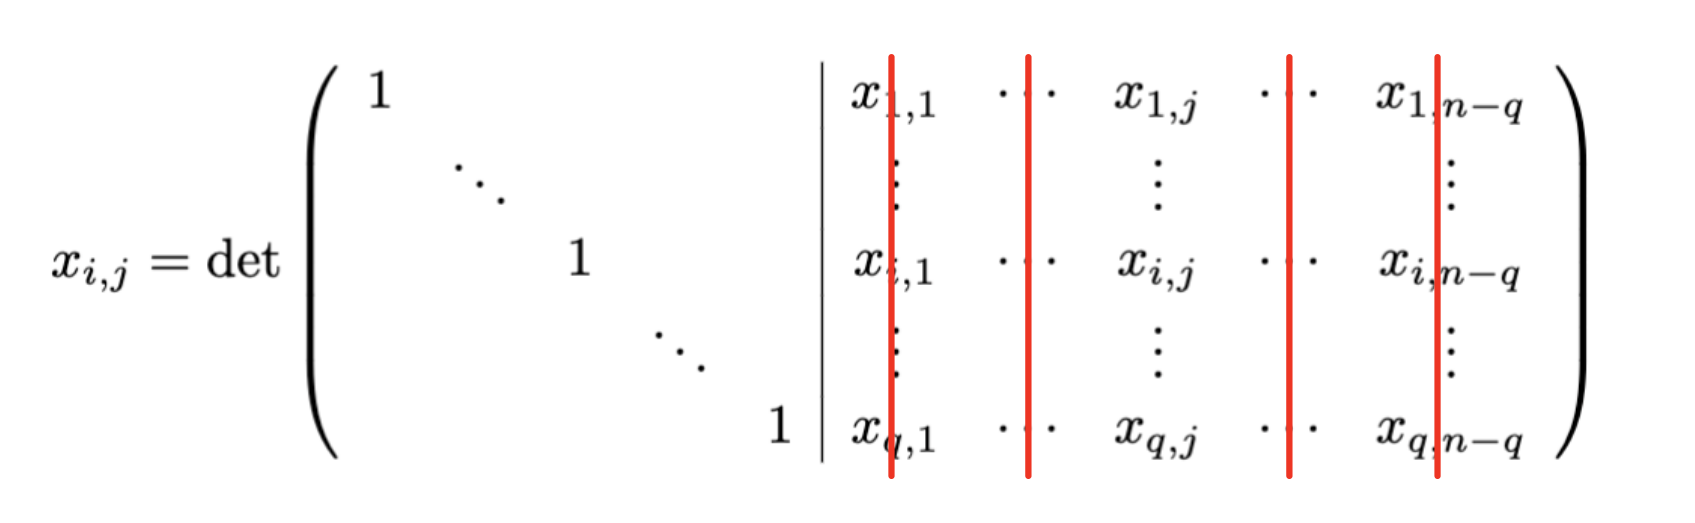
\includegraphics[width=.68\textwidth]{figures/fig-2.2.9.png}

\caption{去掉第 $i$ 列以及 $q+1,\ldots,n$ 中除 $q+j$ 外的所有列, 所得子式恰为 $x_{i,j}$.}\label{src:2.2.9}
\end{figure}
\[
x_{i,j}=\det
\left(\begin{array}{ccccc|ccccc}
1&&&&&x_{1,1}&\cdots&x_{1,j}&\cdots&x_{1,n-q}\\
&\ddots&&&&\vdots&&\vdots&&\vdots\\
&&1&&&x_{i,1}&\cdots&x_{i,j}&\cdots&x_{i,n-q}\\
&&&\ddots&&\vdots&&\vdots&&\vdots\\
&&&&1&x_{q,1}&\cdots&x_{q,j}&\cdots&x_{q,n-q}
\end{array}\right)
\]
\begin{exercise}[适合练习]\label{src:2.2.10}
对域 $k$, 定义 $\Gr(q,n)_k:=\Gr(q,n)\times_{\mathbb Z}k$, 取对应于商 $Q=k^n/K$ 的点 $p\in\Gr(q,n)_k$.
证明切空间与 $k$-线性映射 $K\to Q$ 的向量空间之间存在自然双射
\[
T_p(\Gr(q,n)_k)\xrightarrow{\sim}\operatorname{Hom}_k(K,Q).
\]
\end{exercise}
\begin{exercise}[适合练习]\label{src:2.2.11}
利用 $\Gr(q,n)$ 的固有性赋值判别法(习题~\bookref{2.2.7}), 给出射影性的另一证明.
\end{exercise}
\begin{exercise}[困难]\label{src:2.2.12}
证明 $\Gr(q,n)$ 可等同于商 $U/\operatorname{GL}_q$, 其中 $U\subseteq\mathbb A^{q\times n}$ 为满秩 $q\times n$ 矩阵组成的子集; 也可等同于商 $\operatorname{GL}_n/H$, 其中
\[
H=\left\{\left.
\begin{pmatrix}A&B\\0&C\end{pmatrix}
\ \right|\ A\in\operatorname{GL}_q,\ B\in\mathbb A^{q\times(n-q)},\
C\in\operatorname{GL}_{n-q}\right\}\subseteq\operatorname{GL}_n.
\]
\end{exercise}
\begin{exercise}[困难]\label{src:2.2.13}
证明 $\operatorname{Pic}(\Gr(q,n))\cong\mathbb Z$, 且由 Plücker 线丛生成.
\end{exercise}
\begin{exercise}[旗簇]\label{src:2.2.14}
固定正整数 $n$ 及严格递减的整数序列 $n>q_1>\cdots>q_s>0$.
证明将概形 $S$ 映至商序列
\[
\mathcal O_S^{\oplus n}\twoheadrightarrow V_1\twoheadrightarrow
\cdots\twoheadrightarrow V_s
\]
的同构类的函子 $\Sch\to\Sets$, 可由 $\mathbb Z$ 上的射影概形表出, 其中每个 $V_i$ 都是 $S$ 上秩为 $q_i$ 的向量丛.
\end{exercise}
\subsection{相对版本}\label{src:2.2.3-subsection}
我们证明: 对 Noether 概形 $S$ 上任意向量丛 $V$, 函子 $\Gr(q,V)$ 在 $S$ 上可表且射影.
\begin{proof}[定理~\bookref{2.1.1}~的证明]
若 $V$ 为 $S$ 上秩为 $n$ 的向量丛, 则有相对 Plücker 嵌入
\[
\begin{aligned}
P:\Gr(q,V)&\longrightarrow\mathbb P\left(\bigwedge^qV\right),\\
[V_T\twoheadrightarrow Q]&\longmapsto
\left[\bigwedge^qV_T\longrightarrow\bigwedge^qQ\right],
\end{aligned}
\]
上式定义在 $S$-概形 $T$ 上, 是 $S$ 上的函子态射.
由于 $\mathbb P(\bigwedge^qV)$ 在 $S$ 上射影, 只需证明这一态射可由闭浸入表出.
这一性质可在 Zariski 局部检验: 若 $U\subseteq S$ 为使 $V$ 平凡的开子概形, 则 $\Gr(q,V)\to\mathbb P(\bigwedge^qV)$ 在 $U$ 上的限制, 是 Plücker 嵌入
$\Gr(q,\mathcal O_U^{\oplus n})\to\mathbb P(\bigwedge^q\mathcal O_U^{\oplus n})$
沿 $U\to\operatorname{Spec}\mathbb Z$ 的基变换; 我们已验证后者是闭浸入(命题~\bookref{2.2.8}).
\end{proof}
由于 Grassmann 函子可表, 存在万有族(见定义~\bookref{1.3.25}), 即存在万有商
$\mathcal O_{\Gr(q,V)}\otimes_SV\to Q^{\mathrm{univ}}$, 
其中 $\mathcal O_{\Gr(q,V)}\otimes_SV$ 表示 $V$ 沿结构态射 $\Gr(q,V)\to S$ 的拉回.
沿 Plücker 嵌入拉回 $\mathcal O(1)$, 得到 $\det(Q^{\mathrm{univ}})$, 有时称之为\newterm{Plücker 线丛}{Plücker line bundle}.
因此得到: 
\begin{corollary}\label{src:2.2.15}
万有商的行列式 $\det(Q^{\mathrm{univ}})$ 是 $\Gr(q,V)$ 上在 $S$ 上相对非常丰沛的线丛.
\end{corollary}

% Source printed pp. 54-59.
\section{Castelnuovo--Mumford 正则性}\label{src:2.3}
\begin{epigraph}
代数几何中一些最深刻的结果, 涉及给出层的高阶上同调群为 $0$ 的判别准则的问题...我们将在这里(借助 Nakai, Matsusaka 和 Kleiman 发展并使用的技术)只证明一个较弱的消灭定理, 但它能统一地适用于一大类层.
\epigraphauthor{David Mumford~\cite[第 $99$ 页]{Mum66a}}
\end{epigraph}
Serre 消灭定理---有时称为 Cartan--Serre--Grothendieck 定理---断言: 若 $F$ 为射影簇 $(X,\mathcal O_X(1))$ 上的凝聚层, 则当 $d\gg0$ 时, 
\begin{enumerate}[(1)]
\item $F(d)$ 无基点; 
\item 对 $i>0$, $H^i(X,F(d))=0$; 且
\item 对所有 $k\geq0$, 乘法映射
\[
H^0(X,F(d))\otimes H^0(X,\mathcal O(k))
\longrightarrow H^0(X,F(d+k))
\]
满射.
\end{enumerate}
Castelnuovo--Mumford 正则性定量衡量了使扭转 $F(d)$ 满足这三个上同调性质所需的 $d$ 的大小.
\subsection{定义与基本性质}\label{src:2.3.1-subsection}
\begin{definition}\label{src:2.3.1}
设 $F$ 为域 $k$ 上射影空间 $\mathbb P^n$ 的凝聚层.
对整数 $m$, 称 $F$ 为 \newterm{$m$-正则的}{m-regular}, 如果
\[
H^i(\mathbb P^n,F(m-i))=0
\]
对所有 $i\geq1$ 成立.
$F$ 的\newterm{正则性}{regularity}是使 $F(m)$ 为 $m$-正则的最小整数 $m$.
\end{definition}
由正则性的定义可知, 若 $F$ 为 $m$-正则, 则 $F(d)$ 为 $(m-d)$-正则.
我们将在命题~\bookref{2.3.5}~中证明: 若 $F$ 为 $m$-正则, 则对所有 $d\geq m$, 它也是 $d$-正则的.
定义中要求第 $(m-i)$ 次扭转的第 $i$ 上同调消灭, 乍看可能有些神秘, 但这个定义对于按维数归纳的论证很方便, 以下结果就说明了这一点.
\begin{lemma}\label{src:2.3.2}
设 $F$ 为域 $k$ 上 $\mathbb P^n$ 的 $m$-正则凝聚层.
若超平面 $H\subseteq\mathbb P^n$ 避开 $F$ 的伴随点, 则 $F|_H$ 也是 $m$-正则的.
\end{lemma}
\begin{proof}
假设表明, 在仿射开子概形 $U\subseteq\mathbb P^n$ 上, $H$ 的定义方程为模 $\Gamma(U,F)$ 的非零因子.
因此 $H:F(-1)\to F$ 为单射, 且对每个整数 $i>0$, 有短正合列
\[
0\longrightarrow F(m-i-1)\longrightarrow F(m-i)
\longrightarrow F|_H(m-i)\longrightarrow0.
\]
它诱导上同调长正合列
\[
\cdots\longrightarrow H^i(\mathbb P^n,F(m-i))
\longrightarrow H^i(H,F|_H(m-i))
\longrightarrow H^{i+1}(\mathbb P^n,F(m-i-1))\longrightarrow\cdots.
\]
若 $F$ 为 $m$-正则, 则
$H^i(\mathbb P^n,F(m-i))=H^{i+1}(\mathbb P^n,F(m-i-1))=0$.
所以对所有 $i>0$, $H^i(H,F|_H(m-i))=0$, 故 $F|_H$ 也是 $m$-正则的.
\end{proof}
\begin{exercise}[简单, 适合练习]\label{src:2.3.3}
\begin{enumerate}[(a)]
\item 证明 $\mathbb P^n$ 上的 $\mathcal O(d)$ 为 $(-d)$-正则.
\item 证明次数为 $d$ 的超曲面 $H\subseteq\mathbb P^n$ 的结构层为 $(d-1)$-正则.
\item 证明亏格为 $g$ 的光滑曲线 $C\subseteq\mathbb P^n$ 的结构层为 $(2g-1)$-正则.
\end{enumerate}
\end{exercise}
\begin{exercise}[简单]\label{src:2.3.4}
设 $0\to K\to F\to Q\to0$ 为 $\mathbb P^n$ 上凝聚层的短正合列.
若 $K$ 为 $(m+1)$-正则而 $F$ 为 $m$-正则, 证明 $Q$ 为 $m$-正则.
\end{exercise}
正则性的另一个优点是如下 Castelnuovo 的结果.
\begin{proposition}[正则性的性质]\label{src:2.3.5}
设 $F$ 为域 $k$ 上 $\mathbb P^n$ 的 $m$-正则凝聚层.
\begin{enumerate}[(1)]
\item 对 $d\geq m$, $F$ 为 $d$-正则.
\item 若 $d\geq m$ 且 $k\geq0$, 则乘法映射
\[
H^0(\mathbb P^n,F(d))\otimes H^0(\mathbb P^n,\mathcal O(k))
\longrightarrow H^0(\mathbb P^n,F(d+k))
\]
满射.
\item 对 $d\geq m$, $F(d)$ 整体生成, 且对 $i\geq1$, $H^i(\mathbb P^n,F(d))=0$.
\end{enumerate}
\end{proposition}
\begin{proof}
若 $k\to k'$ 为域扩张, 则平坦基变换(\bookref{A.2.12})表明
\[
H^i(\mathbb P_k^n,F)\otimes_k k'
=H^i(\mathbb P_{k'}^n,F\otimes_k k').
\]
由于 $k\to k'$ 忠实平坦, 断言~(1)--(3)~可在基变换后检验.
故可假设 $k$ 代数闭, 特别地, 为无限域.
对~(1)~和~(2), 我们按 $n$ 归纳; 初始情形 $n=0$ 显然成立.
若 $n>0$, 由于 $k$ 无限, 可以选择避开 $F$ 的伴随点的超平面 $H\subseteq\mathbb P^n$.
限制 $F|_H$ 在 $H\cong\mathbb P^{n-1}$ 上为 $m$-正则(引理~\bookref{2.3.2}), 故归纳假设表明~(1)~和~(2)~对 $F|_H$ 成立.

为证明~(1), 还按整数 $d$ 归纳. 初始情形 $d=m$ 由假设成立.
当 $d>m$ 时, 短正合列 $0\to F(d-i-1)\to F(d-i)\to F|_H(d-i)\to0$ 诱导上同调长正合列
\[
\cdots\longrightarrow H^i(\mathbb P^n,F(d-i-1))
\longrightarrow H^i(\mathbb P^n,F(d-i))
\longrightarrow H^i(H,F|_H(d-i))\longrightarrow\cdots.
\]
当 $i>0$ 时, 第一项由关于 $d$ 的归纳假设消灭, 因为 $F$ 为 $(d-1)$-正则.
第三项由关于 $n$ 的归纳假设消灭: 由引理~\bookref{2.3.2}, $F|_H$ 为 $m$-正则, 因而由关于 $n$ 的归纳假设为 $d$-正则, 故 $H^i(H,F|_H(d-i))=0$.
于是第二项消灭, 得证~(1).

为证明~(2), 除 $n$ 外, 我们还按 $k$ 归纳.
将乘法映射记为
\[
\mu_{d,k}:H^0(\mathbb P^n,F(d))\otimes H^0(\mathbb P^n,\mathcal O(k))
\longrightarrow H^0(\mathbb P^n,F(d+k)).
\]
虽然初始情形 $k=0$ 显然成立, 但归纳论证需要直接证明 $k=1$ 的情形.
为此, 考虑交换图
\begin{equation}\label{src:2.3.6}
\begin{tikzcd}[column sep=large,row sep=large,font=\small]
& H^0(\mathbb P^n,F(d))\otimes H^0(\mathbb P^n,\mathcal O(1))
\arrow[r,"\nu_d\otimes\mathrm{res}"]\arrow[d,"\mu_{d,1}"]&
H^0(H,F|_H(d))\otimes H^0(H,\mathcal O_H(1))\arrow[d]\\
H^0(\mathbb P^n,F(d))\arrow[r,"\alpha"]
\arrow[ur,"\mathrm{id}\otimes H"]&
H^0(\mathbb P^n,F(d+1))\arrow[r,"\nu_{d+1}"]&
H^0(H,F|_H(d+1)).
\end{tikzcd}
\end{equation}
映射 $\alpha$ 由乘以 $H\in H^0(\mathbb P^n,\mathcal O(1))$ 给出, 且有包含 $\operatorname{im}(\alpha)\subseteq\operatorname{im}(\mu_{d,1})$.
由于由~(1)~有 $H^1(\mathbb P^n,F(d))=0$, 限制映射 $\nu_d:H^0(\mathbb P^n,F(d))\to H^0(H,F|_H(d))$ 满射.
同样, 由于 $H^1(\mathbb P^n,\mathcal O)=0$, $\mathrm{res}:H^0(\mathbb P^n,\mathcal O(1))\to H^0(H,\mathcal O_H(1))$ 满射, 故上方水平箭头满射.
将归纳假设应用于 $H=\mathbb P^{n-1}$, 可知右方竖直箭头满射.
因此, 复合 $\nu_{d+1}\circ\mu_{d,1}$ 满射, 从而 $\operatorname{im}(\mu_{d,1})$ 满射到 $H^0(H,F|_H(d+1))$.
由下行的正合性, 
\[
\begin{aligned}
H^0(\mathbb P^n,F(d+1))
&=\operatorname{im}(\mu_{d,1})+\ker(\nu_{d+1})\\
&=\operatorname{im}(\mu_{d,1})+\operatorname{im}(\alpha)
=\operatorname{im}(\mu_{d,1}),
\end{aligned}
\]
故 $\mu_{d,1}$ 满射.

若 $k>1$, 考虑交换方形
\[
\begin{tikzcd}[column sep=normal,row sep=large,font=\footnotesize]
H^0(\mathbb P^n,F(d))\otimes H^0(\mathbb P^n,\mathcal O(k-1))
\otimes H^0(\mathbb P^n,\mathcal O(1))
\arrow[r]\arrow[d,"\mu_{d,k-1}\otimes\mathrm{id}"']&
H^0(\mathbb P^n,F(d))\otimes H^0(\mathbb P^n,\mathcal O(k))
\arrow[d,"\mu_{d,k}"]\\
H^0(\mathbb P^n,F(d+k-1))\otimes H^0(\mathbb P^n,\mathcal O(1))
\arrow[r,"\mu_{d+k-1,1}"]&
H^0(\mathbb P^n,F(d+k)).
\end{tikzcd}
\]
分别对 $k-1$ 和 $k=1$ 应用归纳假设, 左方竖直映射和下方水平箭头均满射.
故 $\mu_{d,k}$ 满射.

为证明~(3), 我们知道当 $k\gg0$ 时, $F(d+k)$ 整体生成, 即
$\gamma_{F(d+k)}:H^0(\mathbb P^n,F(d+k))\otimes\mathcal O_{\mathbb P^n}\to F(d+k)$
满射.
考虑交换方形
\[
\begin{tikzcd}[column sep=normal,row sep=large,font=\footnotesize]
H^0(\mathbb P^n,F(d))\otimes H^0(\mathbb P^n,\mathcal O(k))
\otimes\mathcal O_{\mathbb P^n}
\arrow[r,"\mu_{d,k}\otimes\mathrm{id}"]
\arrow[d,"\gamma_{F(d)}\otimes\mathrm{id}"']&
H^0(\mathbb P^n,F(d+k))\otimes\mathcal O_{\mathbb P^n}
\arrow[d,"\gamma_{F(d+k)}"]\\
F(d)\otimes\bigl(H^0(\mathbb P^n,\mathcal O(k))\otimes\mathcal O_{\mathbb P^n}\bigr)
\arrow[r,"\mathrm{id}\otimes\gamma_{\mathcal O(k)}"]&
F(d)\otimes\mathcal O(k).
\end{tikzcd}
\]
由~(2), 上方水平箭头满射, 故从左上到右下的复合满射.
由于下方水平映射由与 $F(d)$ 作张量积定义, 映射 $\gamma_{F(d)}$ 必须满射.
最后, 为说明 $F(d)$ 的高阶上同调消灭, 注意对每个 $i>0$, 由~(1), 层 $F$ 为 $(d+i)$-正则, 故 $H^i(\mathbb P^n,F(d))=0$.
\end{proof}
断言~(1)~的一个直接推论是: 若 $F$ 为 $m$-正则, 则对所有 $d\geq m$, 限制映射
\[
\nu_d::H^0(\mathbb P^n,F(d))\longrightarrow H^0(H,F|_H(d))
\]
满射. 事实上, (1)~表明 $F$ 也为 $d$-正则, 满射性来自 $H^1(\mathbb P^n,F(d-1))$ 的消灭.
以下引理将在定理~\bookref{2.3.8}~的证明中使用, 它表明在较弱的假设下仍可保证 $\nu_d$ 满射.
\begin{lemma}\label{src:2.3.7}
设 $F$ 为 $\mathbb P^n$ 上的凝聚层, $H$ 为避开 $F$ 的伴随点的超平面.
若 $F|_H$ 为 $m$-正则, 且 $\nu_d$ 对某个 $d\geq m$ 满射, 则 $\nu_p$ 对所有 $p\geq d$ 满射.
\end{lemma}
\begin{proof}
观察图~\eqref{src:2.3.6}, 可知上方箭头 $\nu_d\otimes\mathrm{res}$ 满射(因为 $\nu_d$ 和 $\mathrm{res}$ 均满射), 右方竖直乘法态射也满射(对 $m$-正则层 $F|_H$ 应用命题~\bookref{2.3.5}(2)).
这意味着 $\nu_{d+1}$ 满射, 断言由归纳法成立.
\end{proof}
\subsection{正则性的界}\label{src:2.3.2-subsection}
我们证明平凡向量丛的子层的正则性有界, 这一结果由 Mumford 在~\cite[第 $101$ 页]{Mum66a}~中首次建立.
它是代数几何中几乎每个模空间有界性的基础.\footnote{即使在~\cite[Tag 0DPA]{SP}~中使用 Artin 代数性公理(\bookref{C.7.4})构造 Hilbert 概形与 Quot 概形时, 建立拟紧性所用的也是这一结果~\cite[Tag 08AG]{SP}.}
\begin{theorem}[正则性的有界性]\label{src:2.3.8}
对每一对非负整数 $r,n$ 及每个多项式 $P\in\mathbb Q[z]$, 存在整数 $m_0$, 满足如下性质: 对每个域 $k$, 具有 Hilbert 多项式 $P$ 的每个子层 $F\subset\mathcal O_{\mathbb P_k^n}^{\oplus r}$ 都为 $m_0$-正则.
\end{theorem}
\begin{proof}
由于 $m$-正则性不受域扩张影响, 可以假设 $k$ 无限.
我们按 $n$ 归纳. 初始情形 $n=0$ 成立, 因为 $\mathbb P^0$ 上每个层 $F$ 对每个整数 $m$ 都是 $m$-正则的.

设 $n\geq1$, $F\subseteq\mathcal O_{\mathbb P^n}^{\oplus r}$ 具有 Hilbert 多项式 $P$.
可以选择避开 $\mathcal O_{\mathbb P^n}^{\oplus r}/F$ 的所有伴随点的超平面 $H\subseteq\mathbb P^n$.
这保证
$\operatorname{Tor}^{\mathcal O_{\mathbb P^n}}_1
(\mathcal O_H,\mathcal O_{\mathbb P^n}^{\oplus r}/F)=0$, 
且短正合列 $0\to F\to\mathcal O_{\mathbb P^n}^{\oplus r}\to\mathcal O_{\mathbb P^n}^{\oplus r}/F\to0$
限制为短正合列
\begin{equation}\label{src:2.3.9}
0\longrightarrow F|_H\longrightarrow\mathcal O_H^{\oplus r}
\longrightarrow\mathcal O_H^{\oplus r}/F\longrightarrow0.
\end{equation}
由于 $H\cong\mathbb P^{n-1}$, 可以对 $F|_H\subseteq\mathcal O_H^{\oplus r}$ 应用归纳假设.
另一方面, 由于 $F\subseteq\mathcal O_{\mathbb P^n}^{\oplus r}$ 无挠, 有短正合列
\begin{equation}\label{src:2.3.10}
0\longrightarrow F(-1)\xrightarrow{H}F\longrightarrow F|_H\longrightarrow0.
\end{equation}
$F|_H$ 的 Hilbert 多项式为
\[
\chi(F|_H(d))=\chi(F(d))-\chi(F(d-1))=P(d)-P(d-1).
\]
特别地, $F|_H$ 的 Hilbert 多项式仅依赖于 $P$.
对 $F|_H\subseteq\mathcal O_H^{\oplus r}$ 应用归纳假设, 得到整数 $m_1$, 使 $F|_H$ 为 $m_1$-正则.

对 $m\geq m_1$, 由于 $F|_H$ 为 $m$-正则, 故也为 $(m+1)$-正则, 因此对所有 $i\geq1$, 
\[
H^i(H,F|_H(m-i))=H^{i+1}(H,F|_H(m-(i+1)))=0.
\]
将~\eqref{src:2.3.10}~扭转 $m-i$ 后所诱导的上同调长正合列, 表明
\[
H^{i+1}(\mathbb P^n,F(m-(i+1)))
\xrightarrow{\sim}H^{i+1}(\mathbb P^n,F(m-i)).
\]
由于 $H^{i+1}(\mathbb P^n,F(d))$ 在 $d\gg0$ 时消灭, 可以断言: 对 $m\geq m_1$, $F$ 满足上同调次数至少为 $2$ 的 $m$-正则性条件.

为处理 $H^1$, 注意当 $m\geq m_1-1$ 时, 长正合列
\begin{equation}\label{src:2.3.11}
\begin{aligned}
0&\longrightarrow H^0(\mathbb P^n,F(m-1))
\longrightarrow H^0(\mathbb P^n,F(m))
\longrightarrow H^0(H,F|_H(m))\\
&\longrightarrow H^1(\mathbb P^n,F(m-1))
\longrightarrow H^1(\mathbb P^n,F(m))
\longrightarrow H^1(H,F|_H(m))=0
\end{aligned}
\end{equation}
给出不等式 $h^1(\mathbb P^n,F(m_1-2))\geq h^1(\mathbb P^n,F(m_1-1))\geq\cdots$, 它们最终稳定为 $0$.
我们断言, 事实上, 在达到 $0$ 之前, 不等式
$h^1(\mathbb P^n,F(m_1-2))>h^1(\mathbb P^n,F(m_1-1))>\cdots$
都是严格的.
为说明这一点, 注意当 $m\geq m_1-1$ 时, 
$h^1(\mathbb P^n,F(m-1))=h^1(\mathbb P^n,F(m))$
当且仅当 $\nu_m:H^0(\mathbb P^n,F(m))\to H^0(H,F|_H(m))$ 满射.
假设对某个 $m'\geq m$, $\nu_{m'}$ 满射.
由于 $F|_H$ 为 $m_1$-正则, 可用引理~\bookref{2.3.7}~推出: 对所有 $m''\geq m'$, $\nu_{m''}$ 满射.
因此 $h^1(\mathbb P^n,F(m''))$ 对 $m''\geq m'$ 为常数, 故为零.
断言得证. 令 $m_2=m_1+h^1(\mathbb P^n,F(m_1))$, 则
$h^1(\mathbb P^n,F(m_2-1))=0$, 故 $F$ 为 $m_2$-正则.

还需证明 $m_2$ 被一个不依赖于 $F$ 的常数 $m_0$ 控制.
由于 $F\subseteq\mathcal O_{\mathbb P^n}^{\oplus r}$, 对任意 $d\geq0$, 
$h^0(\mathbb P^n,F(d))\leq rh^0(\mathbb P^n,\mathcal O(d))=r\binom{n+d}{n}$.
利用 $i\geq2$ 时 $h^i(\mathbb P^n,F(m_1))$ 的消灭, 得到
\[
\begin{aligned}
h^1(\mathbb P^n,F(m_1))
&=h^0(\mathbb P^n,F(m_1))-\chi(F(m_1))\\
&\leq r\binom{n+m_1}{n}-P(m_1).
\end{aligned}
\]
定义 $m_0:=m_1+1+r\binom{n+m_1}{n}-P(m_1)\geq m_2$, 
就得到所需的常数, 使具有 Hilbert 多项式 $P$ 的每个 $F\subseteq\mathcal O_{\mathbb P^n}^{\oplus r}$ 均为 $m_0$-正则.
\end{proof}
\begin{remark}\label{src:2.3.12}
上述证明实际上建立了一个更强的断言.
为陈述这一结果, 回忆: 每个次数为 $n$ 的数值多项式 $P\in\mathbb Q[z]$(即对整数 $d\gg0$, 有 $P(d)\in\mathbb Z$)均可唯一写成
\[
P(d)=\sum_{i=0}^na_i\binom di,\qquad a_i\in\mathbb Z.
\]
这可由直接的归纳论证得到, 参见~\cite[命题 I.7.3]{Har77}.
对非负整数 $r,n$, 存在多项式
\begin{equation}\label{src:2.3.13}
\Lambda_{r,n}\in\mathbb Z[x_0,\ldots,x_n],
\end{equation}
满足如下性质: 对每个域 $k$, 具有 Hilbert 多项式
$P(d)=\sum_i a_i\binom di$ 的每个子层
$F\subseteq\mathcal O_{\mathbb P_k^n}^{\oplus r}$
均为 $m_0$-正则, 其中 $m_0=\Lambda_{r,n}(a_0,\ldots,a_n)$.
见~\cite[第 $101$ 页]{Mum66a}.
\end{remark}
\begin{exercise}\label{src:2.3.14}
设 $P=d$ 为固定整数 $d$ 对应的常数多项式.
使每个定义长度为 $d$ 的 $0$ 维子概形的理想层 $I\subseteq\mathcal O_{\mathbb P^n}$ 为 $m$-正则的最优 $m$ 是多少?
\end{exercise}
\begin{remark}[最优界]\label{src:2.3.15}
虽然 Mumford 的正则性有界性结果(定理~\bookref{2.3.8})给出了显式界, 且足以用于包括构造 Hilbert 概形在内的许多应用, Gotzmann 建立了更优的界: 
对域 $k$ 上具有 Hilbert 多项式 $P$ 的射影概形 $X\subseteq\mathbb P^N$, 存在唯一的整数
$\lambda_1\geq\lambda_2\geq\cdots\geq\lambda_r\geq1$, 使 $P$ 可写成
\[
P(d)=\binom{d+\lambda_1-1}{\lambda_1-1}
+\binom{d+\lambda_2-2}{\lambda_2-1}
+\cdots+\binom{d+\lambda_r-r}{\lambda_r-1},
\]
且 $X$ 的理想层 $I_X$ 为 $r$-正则.
见~\cite{Got78}, \cite[\S$4.3$]{BH93}, \cite{Gre89}~和~\cite[\S$3$]{Gre98}.
\end{remark}
\begin{exercise}\label{src:2.3.16}
设 $C\subseteq\mathbb P^n$ 为次数 $d$, 亏格 $g$ 的曲线.
证明 Gotzmann 的界表明 $C$ 的理想层 $I_C$ 为 $\bigl(\binom d2+1-g\bigr)$-正则.
能否将它与定理~\bookref{2.3.8}~的证明给出的界比较, 即能否从~\eqref{src:2.3.13}~计算 $\Lambda_{1,n}(1-g,d)$?
\end{exercise}
\begin{remark}\label{src:2.3.17}
\cite{GLP83}~证明了: 次数为 $d$ 的整的非退化曲线 $C\subseteq\mathbb P^N$ 的理想层 $I_C$ 为 $(d-N+2)$-正则.
更一般的猜想断言: 维数 $n$, 次数 $d$ 的光滑非退化射影子簇 $X\subseteq\mathbb P^N$ 的理想层为 $(d-(N-n))+1)$-正则; 见~\cite{GLP83,EG84}.
\end{remark}
\begin{proposition}[族中的正则性]\label{src:2.3.18}
设 $S$ 为 Noether 概形, $\pi:\mathbb P_S^n\to S$ 为相对射影空间, $Q$ 为 $\mathbb P_S^n$ 上在 $S$ 上平坦的凝聚层.
假设存在整数 $m>0$, 使对每个 $s\in S$, 在 $\mathbb P_{\kappa(s)}^n$ 上的限制 $Q_s$ 都为 $m$-正则.
则对 $d\geq m$, 
\begin{enumerate}[(1)]
\item $\pi_*Q(d)$ 为向量丛, 且其构造与沿 $f:T\to S$ 的基变换交换, 即 $f^*\pi_*Q(d)\cong\pi_{T,*}Q_T(d)$; 
\item 对 $i>0$, $R^i\pi_*Q(d)=0$; 且
\item $\pi^*\pi_*Q(d)\to Q(d)$ 满射.
\end{enumerate}
\end{proposition}
\begin{proof}
由于对所有 $s\in S$, 
$R^i\pi_*Q(d)\otimes\kappa(s)\to H^i(\mathbb P_{\kappa(s)}^n,Q_s(d))=0$
满射, 上同调与基变换(\bookref{A.6.8})给出~(1)~和~(2).
对~(3), 令 $C=\operatorname{coker}(\pi^*\pi_*Q(d)\to Q(d))$.
对每个 $s\in S$, 有 Cartesian 图
\[
\begin{tikzcd}
\mathbb P_{\kappa(s)}^n\arrow[r,"j"]\arrow[d,"\pi_s"']
\arrow[dr,phantom,"\square"]&
\mathbb P_S^n\arrow[d,"\pi"]\\
\operatorname{Spec}\kappa(s)\arrow[r,"i"]&S.
\end{tikzcd}
\]
利用~(1), 有
$j^*\pi^*\pi_*Q(d)=\pi_s^*i^*\pi_*Q(d)=\pi_s^*\pi_{s,*}Q_s(d)$.
伴随映射 $\pi^*\pi_*Q(d)\to Q(d)$ 沿 $j$ 的拉回, 对应于伴随映射
$\pi_s^*\pi_{s,*}Q_s(d)\to Q_s(d)$; 
由正则性的性质(\bookref{2.3.5}(3)), 后者满射.
因此, 对所有 $s\in S$, 
$C\otimes\kappa(s)=\operatorname{coker}(\pi_s^*\pi_{s,*}Q_s(d)\to Q_s(d))=0$, 
故 $\pi^*\pi_*Q(d)\to Q(d)$ 满射.
\end{proof}

% Source printed pp. 59-65.
\section{Hilb 与 Quot 的射影性}\label{src:2.4}
\begin{epigraph}
射影几何就是全部几何.
\epigraphauthor{Arthur Cayley}
\end{epigraph}
我们证明 Hilbert 概形和 Quot 概形的射影性(\bookref{2.1.2}~与~\bookref{2.1.3}).
\subsection{线丛直和 \texorpdfstring{$F$}{F} 的特殊情形}\label{src:2.4.1-subsection}
设 $S$ 为 Noether 概形, $\pi:\mathbb P_S^n\to S$ 为相对射影空间.
先考虑凝聚层 $F:=\mathcal O_{\mathbb P_S^n}(-l)^{\oplus r}$ 的特殊情形, 其中 $l$ 和 $r\geq1$ 为整数.
对每个整数 $d\geq0$, 可以尝试定义函子态射
\[
\begin{aligned}
\Quot^P(F/\mathbb P_S^n)&\longrightarrow\Gr(P(d),\pi_*F(d)),\\
[F_T\twoheadrightarrow Q]&\longmapsto
[\pi_{T,*}F_T(d)\to\pi_{T,*}Q(d)],
\end{aligned}
\]
其中 $[F_T\twoheadrightarrow Q]$ 为 $S$-概形 $T$ 上的对象.
\begin{enumerate}[步骤 1: ]
\item\label{step:quot-1}
\textit{存在整数 $m_0$, 使对 $d\geq m_0$, 
$\Quot^P(F/\mathbb P_S^n)\to\Gr(P(d),\pi_*F(d))$ 良定义.}
\begin{proof}
由于 $F=\mathcal O_{\mathbb P_S^n}(-l)^{\oplus r}$, 对 $d\geq l$, 
$\pi_*F(d)=(\operatorname{Sym}^{d-l}\Gamma(S,\mathcal O_S))^{\oplus r}$
为向量丛, 且其构造与沿 $T\to S$ 的基变换交换; 对所有 $i>0$, $R^i\pi_*F(d)=0$.
对每个域值点 $s\in S(k)$ 和 Hilbert 多项式为 $P$ 的商
$F_s=\mathcal O_{\mathbb P_k^n}(-l)^{\oplus r}\twoheadrightarrow Q$, 
令 $K_s=\ker(F_s\to Q)$.
则 $K(l)$ 为 $\mathcal O_{\mathbb P_k^n}^{\oplus r}$ 的子层, 其 Hilbert 多项式由 $P$ 和 $\mathcal O_{\mathbb P_k^n}^{\oplus r}$ 的 Hilbert 多项式确定.
因此可由正则性的有界性(\bookref{2.3.8})选取 $m_0\geq l$, 使每个这样的核 $K_s$ 均为 $m_0$-正则.
必要时增大 $m_0$, 还可使 $F_s$ 为 $m_0$-正则.
习题~\bookref{2.3.4}~表明每个商 $Q$ 均为 $m_0$-正则.
由族中的正则性(\bookref{2.3.18}(1)), 对每个 $d\geq m_0$ 及在 $T$ 上平坦, Hilbert 多项式为 $P$ 的商层 $F_T\twoheadrightarrow Q$, 
$\pi_{T,*}Q(d)$ 为 $T$ 上秩为 $P(d)$ 的向量丛, 且其构造与基变换交换.
由于 $F_T$ 和 $Q$ 在 $T$ 上平坦, $K:=\ker(F_T\to Q)$ 也在 $T$ 上平坦.
每个纤维 $K_s$ 为 $m_0$-正则, 故族中的正则性(\bookref{2.3.18}(2))表明: 对 $d\geq m_0$, $R^1\pi_{T,*}K(d)=0$.
因此 $\pi_{T,*}F_T(d)\to\pi_{T,*}Q(d)$ 满射, 且~\bookeqref{2.4.1}~良定义.
\end{proof}
\item\label{step:quot-2}
\textit{存在整数 $m_0$, 使对 $d\geq m_0$, 
$\Quot^P(F/\mathbb P_S^n)\to\Gr(P(d),\pi_*F(d))$ 为单态射.}
\begin{proof}
设 $F_T\twoheadrightarrow Q$ 为在概形 $T$ 上平坦, Hilbert 多项式为 $P$ 的商层.
核 $K=\ker(F_T\to Q)$ 也在 $T$ 上平坦.
按步骤~\ref{step:quot-1}~选取 $m_0$, 则对每个 $s\in S$, 纤维 $K_s$, $(F_T)_s$ 和 $Q_s$ 均为 $m_0$-正则.
由族中的正则性(\bookref{2.3.18}(2)), 对 $d\geq m_0$, $R^1\pi_{T,*}K(d)=0$, 得到短正合列的交换图
\[
\begin{tikzcd}[column sep=small,row sep=large,font=\small]
0\arrow[r]&\pi_T^*\pi_{T,*}K(d)\arrow[r]\arrow[d]
\arrow[dr,"\alpha"]&
\pi_T^*\pi_{T,*}F_T(d)\arrow[r]\arrow[d]&
\pi_T^*\pi_{T,*}Q(d)\arrow[r]\arrow[d]&0\\
0\arrow[r]&K(d)\arrow[r]&F_T(d)\arrow[r]&Q(d)\arrow[r]&0.
\end{tikzcd}
\]
由族中的正则性(\bookref{2.3.18}(3)), 每个竖直映射均满射.
所以 $Q(d)=\operatorname{coker}(\alpha)$ 由 $\pi_{T,*}F_T(d)\to\pi_{T,*}Q(d)$ 唯一确定.
\end{proof}
\item\label{step:quot-3}
\textit{存在整数 $m_0$, 使对 $d\geq m_0$, 
$\Quot^P(F/\mathbb P_S^n)\to\Gr(P(d),\pi_*F(d))$ 为局部闭浸入.}
\begin{proof}
设 $T\to\Gr(P(d),\pi_*F(d))$ 为由向量丛商
$(\pi_*F(d))_T=\pi_{T,*}F_T(d)\twoheadrightarrow V$
确定的映射, 记其核为 $K$.
考虑纤维积
\[
\begin{tikzcd}[column sep=large]
Y\arrow[r]\arrow[d]\arrow[dr,phantom,"\square"]&
T\arrow[d,"{[\pi_{T,*}F_T(d)\twoheadrightarrow V]}"]\\
\Quot^P(F/\mathbb P_S^n)\arrow[r]&\Gr(P(d),\pi_*F(d)).
\end{tikzcd}
\]
在 $\mathbb P_T^n$ 上, 有层的交换图
\[
\begin{tikzcd}[column sep=small,row sep=large]
0\arrow[r]&\pi_T^*K\arrow[r]\arrow[dr,"\alpha"]&
\pi_T^*\pi_{T,*}F_T(d)\arrow[r]\arrow[d]&
\pi_T^*V\arrow[r]\arrow[d]&0\\
&&F_T(d)\arrow[r]&Q(d)\arrow[r]&0,
\end{tikzcd}
\]
其中 $Q$ 定义为使 $Q(d)=\operatorname{coker}(\alpha)$.
由于 $K$ 为 $T$ 上的向量丛, $K=\pi_{T,*}\pi_T^*K$, 故 $\pi_{T,*}\alpha$ 等同于包含映射 $K\hookrightarrow\pi_{T,*}F_T(d)$.
对下行应用 $\pi_{T,*}$, 并利用 $R^1\pi_{T,*}(\pi_T^*K)=0$, 得到短正合列
\[
0\longrightarrow K=\pi_{T,*}\pi_T^*K
\longrightarrow\pi_{T,*}F_T(d)\longrightarrow\pi_{T,*}Q(d)
\longrightarrow0.
\]
这给出等同 $\pi_{T,*}Q(d)=V$.

若 $Q$ 在 $T$ 上平坦且具有 Hilbert 多项式 $P$, 则
$[F_T\twoheadrightarrow Q]:T\to\Quot^P(F/\mathbb P_S^n)$
给出原映射 $[\pi_{T,*}F_T(d)\twoheadrightarrow V]:T\to\Gr(P(d),\pi_*F(d))$ 的提升, 换言之, $Y\xrightarrow{\sim}T$ 为同构.
上述分析表明, $Y$ 等同于以下 $T$ 的子函子: 
\[
\begin{aligned}
\Sch/T&\longrightarrow\Sets,\\
(T'\to T)&\longmapsto
\begin{cases}
\{*\},&\text{若 $Q_{T'}$ 在 $T'$ 上平坦且 Hilbert 多项式为 $P$; }\\
\varnothing,&\text{否则.}
\end{cases}
\end{aligned}
\]
平坦化分层的存在性\footnote{平坦化分层的存在性可以说是 Quot 概形射影性(\bookref{2.1.3})证明中最深刻的组成部分.}(\bookref{A.2.16})表明, $Y$ 可由 $T$ 的局部闭子概形表出.
\end{proof}
\end{enumerate}
将结论概括如下: 
\begin{proposition}\label{src:2.4.1}
设 $S$ 为 Noether 概形, $\pi:\mathbb P^n\to S$ 为相对射影空间.
若 $F:=\mathcal O_{\mathbb P_S^n}(-l)^{\oplus r}$ 且 $P\in\mathbb Q[z]$, 则存在整数 $m_0$, 使对所有 $d\geq m_0$, 
\[
\Quot^P(F/\mathbb P_S^n)\longrightarrow\Gr(P(d),\pi_*F(d))
\]
为局部闭浸入. 特别地, $\Quot^P(F/\mathbb P_S^n)$ 可由 $S$ 上的拟射影概形表出.
\end{proposition}
\subsection{Hilb 与 Quot 的赋值判别法}\label{src:2.4.2-subsection}
为建立 Quot 的射影性, 只需知道它固有.
\begin{proposition}\label{src:2.4.2}
对每个 Noether 概形 $S$, $\mathbb P_S^n$ 上的凝聚层 $F$ 和多项式 $P\in\mathbb Q[z]$, 函子 $\Quot^P(F/\mathbb P_S^n)$ 满足 $S$ 上的固有性赋值判别法.
即对每个 $S$ 上分式域为 $K$ 的离散赋值环 $R$, $\mathbb P_K^n$ 上 Hilbert 多项式为 $P$ 的每个平坦凝聚商 $F_K\to Q$, 都唯一延拓为 $\mathbb P_R^n$ 上 Hilbert 多项式为 $P$ 的平坦凝聚商 $F_R\to\widetilde Q$.
\end{proposition}
\begin{remark}\label{src:2.4.3}
换言之, 该命题表明每个交换图
\[
\begin{tikzcd}
\operatorname{Spec}K\arrow[r,"Q"]\arrow[d]&
\Quot^P_{X/S}(F)\arrow[d]\\
\operatorname{Spec}R\arrow[r]\arrow[ur,dashed,"\widetilde Q"]&S
\end{tikzcd}
\]
都有唯一提升. 函子和叠的赋值判别法将在 \S\bookref{4.8} 讨论.
\end{remark}
\begin{proof}
记开浸入为 $j:X_K\hookrightarrow X_R$, 将 $\widetilde Q$ 定义为复合
$F_R\to j_*F_K\to j_*Q$ 的像, 其中第一个映射由伴随映射
$F_R\to j_*j^*F_R=j_*F_K$ 给出.
由于 $\widetilde Q$ 为 $j_*Q$ 的子层, 它在 $R$ 上无挠, 故平坦(因为 $R$ 为离散赋值环).
最后, 由于 $Q$ 在 $R$ 上平坦且 $\operatorname{Spec}R$ 连通, 其 Hilbert 多项式为常数.
\end{proof}
\begin{remark}\label{src:2.4.4}
对 $\Hilb^P_{X/S}$, 上述论证变为: 闭子概形 $Z\subseteq X_K$ 的唯一延拓为概形论像
$\widetilde Z=\operatorname{im}(Z\to X_K\hookrightarrow X_R)$.
概形 $\widetilde Z$ 在 $R$ 上平坦, 因为其所有伴随点都位于 $\operatorname{Spec}R$ 的一般点之上.
\end{remark}
\subsection{射影性}\label{src:2.4.3-subsection}
以下结果完成定理~\bookref{2.1.2}~和~\bookref{2.1.3}~的证明.
\begin{theorem}\label{src:2.4.5}
设 $S$ 为 Noether 概形, $\pi:\mathbb P^n\to S$ 为相对射影空间.
若 $F:=\mathcal O_{\mathbb P_S^n}(-l)^{\oplus r}$ 且 $P\in\mathbb Q[z]$, 则存在整数 $m_0$, 使对所有 $d\geq m_0$, 
\[
\Quot^P(F/\mathbb P_S^n)\longrightarrow\Gr(P(d),\pi_*F(d))
\]
为闭浸入. 特别地, $\Quot^P(F/\mathbb P_S^n)$ 可由 $S$ 上的射影概形表出.
\end{theorem}
\begin{proof}
设 $S$ 为 Noether 概形, $\pi:\mathbb P_S^n\to S$ 为相对射影空间, $F$ 为 $\mathbb P_S^n$ 上任意凝聚层.
选择整数 $l,r$ 及满射 $G:=\mathcal O_{\mathbb P_S^n}(-l)^{\oplus r}\twoheadrightarrow F$, 得到函子态射
\[
\begin{aligned}
\Quot^P(F/\mathbb P_S^n)&\longrightarrow\Quot^P(G/\mathbb P_S^n),\\
[F_T\to Q]&\longmapsto[G_T\twoheadrightarrow F_T\twoheadrightarrow Q],
\end{aligned}
\]
上式定义在 $S$-概形 $T$ 上.
由命题~\bookref{2.4.1}, 函子 $\Quot^P(G/\mathbb P_S^n)$ 可由 $S$ 上的拟射影概形表出; 由命题~\bookref{2.4.2}, 它在 $S$ 上固有, 故射影.

为证明 $\Quot^P(F/\mathbb P_S^n)$ 在 $S$ 上射影, 只需证明上述态射可由闭浸入表出.
这归结为如下断言: 对 $S$-概形 $T$ 及 $Q$ 在 $T$ 上平坦的商 $G_T\twoheadrightarrow Q$, 存在闭子概形 $Z\subseteq T$, 使态射 $T'\to T$ 经 $Z$ 分解当且仅当 $G_{T'}\to Q_{T'}$ 经 $F_{T'}$ 分解.
定义 $K=\ker(G_T\to F_T)$, 考虑图
\[
\begin{tikzcd}
0\arrow[r]&K\arrow[r]\arrow[dr]&G_T\arrow[r]\arrow[d,two heads]&F_T\arrow[r]&0\\
&&Q&&
\end{tikzcd}
\]
则 $G_{T'}\to Q_{T'}$ 经 $F_{T'}$ 分解当且仅当 $K_{T'}\to Q_{T'}$ 为零.
由习题~\bookref{1.3.23}, 参数化使 $K_{T'}\to Q_{T'}$ 为零的映射 $T'\to T$ 的 $T$ 的子函子, 可由闭子概形表出.
\end{proof}
取上述证明中的满射 $G=\mathcal O_{\mathbb P_S^n}(-l)^{\oplus r}\twoheadrightarrow F$.
当 $d\gg0$ 时, 有闭浸入的复合
\[
\begin{aligned}
\Quot^P(F/\mathbb P_S^n)&\hookrightarrow\Quot^P(G/\mathbb P_S^n)
\hookrightarrow\Gr(P(d),\pi_*G(d))\\
&\hookrightarrow\mathbb P\left(\bigwedge^{P(d)}\pi_*G(d)\right).
\end{aligned}
\]
在 $\mathbb P_S^n\times_S\Quot^P(F/\mathbb P_S^n)$ 上, 将万有商记为
\[
F_{\Quot^P(F/\mathbb P_S^n)}\longrightarrow Q^{\mathrm{univ}}.
\]
沿上述复合拉回 $\mathcal O(1)$, 得到 $\det p_{2,*}(Q^{\mathrm{univ}}(d))$.
概括如下: 
\begin{corollary}\label{src:2.4.6}
当 $d\gg0$ 时, $\Quot^P(F/\mathbb P_S^n)$ 上的线丛
$\det\bigl(p_{2,*}(Q^{\mathrm{univ}}(d))\bigr)$ 在 $S$ 上相对非常丰沛.
\end{corollary}
\subsection{推广}\label{src:2.4.4-subsection}
我们首先考虑的推广是旗概形.
\begin{exercise}[旗概形]\label{src:2.4.7}
设 $S$ 为 Noether 概形, $F$ 为 $\mathbb P_S^n$ 上的凝聚层, 且可对某些 $l,r$ 写成 $\mathcal O_{\mathbb P_S^n}(-l)^{\oplus r}$ 的商.
对每个多项式序列 $P_1,\ldots,P_k\in\mathbb Q[z]$, 证明函子
\[
\begin{aligned}
\operatorname{Flag}^{P_1,\ldots,P_k}(F/\mathbb P_S^n/S):
\Sch/S&\longrightarrow\Sets,\\
(T\to S)&\longmapsto
\left\{\begin{array}{l}
\text{$\mathbb P_T^n$ 上拟凝聚层的滤过 $0=F_0\subseteq\cdots\subseteq F_k=F_T$, }\\
\text{其中每个商 $F^i/F^{i-1}$ 为有限表现的 $\mathcal O_{\mathbb P_T^n}$-模, }\\
\text{且在 $T$ 上平坦, 具有 Hilbert 多项式 $P_i$}
\end{array}\right\}
\end{aligned}
\]
可由 $S$ 上的射影概形表出.

提示: 将旗概形构造为相对 Quot 概形的迭代.
即考虑 $\operatorname{Flag}:=\operatorname{Flag}^{P_2,\ldots,P_k}(F/\mathbb P_S^n/S)$, 以及
$\mathbb P_S^n\times_S\operatorname{Flag}$ 上的万有滤过
$0=F_{\mathrm{univ},0}\subseteq F_{\mathrm{univ},2}\subseteq\cdots\subseteq p_1^*F$, 
并证明
\[
\operatorname{Flag}^{P_1,\ldots,P_k}(F/\mathbb P_S^n/S)
\cong\Quot^{P_1}(F_{\mathrm{univ},2}/\operatorname{Flag}/S).
\]
\end{exercise}
定理~\bookref{2.1.3}~对 $\mathbb P_S^n$ 上可写成 $\mathcal O_{\mathbb P_S^n}(-l)^{\oplus r}$ 的商的凝聚层 $F$, 证明了 Quot 概形 $\Quot^P(F/\mathbb P_S^n)$ 的存在性与射影性.
现在考虑更一般的情形.
回忆, 态射 $X\to S$ 有三种不同的射影性概念, 按一般性递增列举如下: 
\begin{itemize}
\item $X\to S$ 分解为闭浸入 $X\hookrightarrow\mathbb P_S^n$ 及 $\mathbb P_S^n\to S$; 有时称为 \newterm{$H$-射影}{H-projective}, 因为这是~\cite[II.4]{Har77}~采用的定义; 
\item $X\to S$ 分解为闭浸入 $X\hookrightarrow\mathbb P(E)$ 及 $\mathbb P(E)\to S$, 其中 $E$ 为 $S$ 上的向量丛; 称为\newterm{强射影}{strongly projective}; 
\item $X\to S$ 分解为闭浸入 $X\hookrightarrow\mathbb P(E)$ 及 $\mathbb P(E)\to S$, 其中 $E$ 为 $S$ 上的有限型拟凝聚层(当 $S$ 为 Noether 概形时, 即凝聚层); 这是~\cite[\S II.5]{EGA}~和~\cite[Tag 01W8]{SP}~的定义.
\end{itemize}
若 $S$ 具有\newterm{消解性质}{resolution property}, 即每个凝聚层都是某个向量丛的商, 则射影态射为强射影态射.
每个光滑概形或拟射影概形都具有这一性质.
Hilbert 函子 $\Hilb^P(X/S)$ 和 Quot 函子 $\Quot^P(F/X/S)$ 的定义, 可扩展至任意射影态射 $X\to S$ 及 $X$ 上的有限型拟凝聚层 $F$.
\begin{exercise}\label{src:2.4.8}
设 $X\to S$ 为概形的射影态射, $F$ 为 $X$ 上的凝聚层.
\begin{enumerate}[(a)]
\item (简单)若 $X\to S$ 为 $H$-射影且 $F$ 为 $\mathcal O_X(-l)^{\oplus r}$ 的商, 证明 $\Quot^P(F/X/S)$ 为 $H$-射影.
\item (中等)若 $f:X\to S$ 为强射影且 $F$ 为 $f^*V\otimes\mathcal O_X(-l)$ 的商, 其中 $V$ 为 $S$ 上的向量丛, 证明 $\Quot^P(F/X/S)$ 为强射影.
\item (中等)若 $X\to S$ 射影, 证明 $\Quot^P(F/X/S)$ 为 $S$ 上的固有概形.
\item (困难)若 $X\to S$ 射影且 $F$ 在 $S$ 上平坦, 证明 $\Quot^P(F/X/S)$ 射影.
\item (未解决)若 $X\to S$ 射影, $\Quot^P(F/X/S)$ 是否总是射影的?
\end{enumerate}
另见~\cite[定理 $2.6$]{AK80}~和~\cite[定理 $5.2$]{Nit05}.
\end{exercise}
\begin{exercise}[困难]\label{src:2.4.9}
设 $X\to S$ 为 Noether 概形的强拟射影态射, 即存在局部闭浸入 $X\hookrightarrow\mathbb P(V)$, 其中 $V$ 为 $S$ 上的向量丛.
若 $F$ 为 $X$ 上的凝聚层, $P\in\mathbb Q[z]$ 为多项式, 可以如下修改 Quot 函子: 
\[
\begin{aligned}
\Quot^P(F/X/S):\Sch/S&\longrightarrow\Sets,\\
(T\to S)&\longmapsto
\left\{\begin{array}{l}
\text{$X_T$ 上有限表现的拟凝聚商 $F_T\to Q$, }\\
\text{在 $T$ 上平坦且支集在 $T$ 上固有, }\\
\text{使每个 $t\in T$ 对应的 $X_t$ 上的 $Q_t$}\\
\text{都具有 Hilbert 多项式 $P$}
\end{array}\right\}.
\end{aligned}
\]
类似地, Hilbert 函子 $\Hilb^P(X/S)$ 定义为只参数化支集在基底上固有的闭子概形.
证明 $\Hilb^P_{X/S}$ 和 $\Quot^P_{X/S}(F)$ 可由 $S$ 上的强拟射影概形表出.
另见~\cite[\S$4$]{FGAIV}, \cite[定理 $2.6$]{AK80}~或~\cite[\S$6$]{Nit05}.
\end{exercise}
\begin{remark}\label{src:2.4.10}
若 $X\to S$ 仅为 Noether 概形的分离态射, 则去掉关于 Hilbert 多项式 $P$ 的条件后, 也可如上定义函子 $\Hilb(X/S)$ 和 $\Quot(F/X/S)$.
Artin 代数性公理(\bookref{C.7.4})可用于证明这些函子可由 $S$ 上分离且局部有限型的代数空间表出; 见~\cite[定理 $6.1$]{Art69b}~和~\cite[Tag 09TQ]{SP}, 或作为特殊情形的定理~\bookref{C.7.7}.
Hironaka 的例子给出 $\mathbb C$ 上光滑固有(但非射影)的三维簇 $X$, 使 $\Hilb(X/S)$ 不是概形.
\end{remark}
\subsection{Chow 簇及其他变体}\label{src:2.4.5-subsection}
\newterm{Chow 簇}{Chow variety}是 Hilbert 概形的一种变体, 较易构造, 但函子性质不如后者良好.
Chow 簇 $\operatorname{Chow}_{r,d}(\mathbb P_k^n)$ 参数化 $\mathbb P_k^n$ 上维数为 $r$, 次数为 $d$ 的有效闭链, 可利用有效闭链 $\alpha$ 的 Chow 形式 $\operatorname{Chow}_\alpha$ 构造.
对有效闭链 $\alpha=\sum_i a_i[X_i]$, 可定义
$\operatorname{Chow}_\alpha=\prod_i\operatorname{Chow}_{X_i}^{a_i}$, 
所以只需对维数 $r$, 次数 $d$ 的整闭子概形 $X\subseteq\mathbb P_k^n$ 定义 Chow 形式.
有定理断言, 轨迹
\begin{equation}\label{src:2.4.11}
\{V\in\Gr(r+1,n+1)\mid X\cap V\neq\varnothing\}
\subseteq\Gr(r+1,n+1)
\end{equation}
为次数 $d$ 的不可约超曲面, 且由多项式
\[
\operatorname{Chow}_X\in
H^0(\Gr(r+1,n+1),\mathcal O_{\Gr}(d))
\cong\operatorname{Sym}^d(\bigwedge^{r+1}k^{n+1})
\]
定义, 该多项式在相差非零常数倍的意义下唯一; 见~\cite[\S$3$, 命题 $2.1$--$2.2$]{GKZ08}.

Chow 簇 $\operatorname{Chow}_{r,d}(\mathbb P^n)$ 是 $\mathbb P^n$ 上所有维数 $r$, 次数 $d$ 的有效闭链的 Chow 形式的集合的闭包.
特征 $0$ 中的主要存在性定理断言: 
\begin{itemize}
\item $\operatorname{Chow}_{r,d}(\mathbb P^n)$ 射影且半正规(即每个在剩余域上诱导同构的有限双射态射 $Y\to\operatorname{Chow}_{r,d}(\mathbb P^n)$ 都是同构); 
\item $\operatorname{Chow}_{r,d}(\mathbb P^n)$ 表出半正规 $k$-概形范畴上的一个函子: 
对半正规 $k$-概形 $S$, $\operatorname{Mor}(S,\operatorname{Chow}_{r,d}(\mathbb P^n))$ 等同于 $\mathbb P_S^n$ 上维数 $r$, 次数 $d$ 的良定义的有效代数闭链族; 且
\item 对多项式 $P(t)=d\cdot t^r/r!+\text{(低次项)}$, 存在从 $\Hilb^P(\mathbb P^n)$ 的半正规化出发的 Hilbert--Chow 态射
\[
\Hilb^P(\mathbb P^n)^{\mathrm{sn}}
\longrightarrow\operatorname{Chow}_{r,d}(\mathbb P^n).
\]
它将闭子概形 $Z\subset\mathbb P^n$ 映至闭链 $a_i[Z_i]$, 其中 $Z_i$ 为第 $i$ 个不可约分支的约化概形结构, $a_i$ 为 $Z_i$ 在其一般点处的重数.
\end{itemize}
见~\cite{CW37}, \cite[\S X.6--8]{HP47}~和~\cite{Sam55}, 或现代论述~\cite[\S$5.4$]{GIT}~和~\cite[I.3.21, I.6.1]{Kol96}.
在概述 $\overline M_g$ 的 GIT 构造时, 我们将使用 $\mathbb P^n$ 中曲线的 Chow 簇(即 $r=1$ 的情形), 此时上述断言的证明稍容易些.
\begin{example}[更多变体]\label{src:2.4.12}
还有进一步的变体和推广.
例如, Vistoli 构造了参数化到分离概形 $X$ 的有限非分歧态射的 Hilbert 叠~\cite{Vis91}.
Alexeev 和 Knutson 的分支簇的模参数化从几何约化概形到分离概形 $X$ 的有限态射~\cite{AK10}.
\end{example}
\begin{exercise}[态射概形]\label{src:2.4.13}
对 Noether 概形的强射影态射 $X\to S$ 和 $Y\to S$, 考虑函子
\[
\begin{aligned}
\operatorname{Mor}_S(X,Y):\Sch/S&\longrightarrow\Sets,\\
(T\to S)&\longmapsto\operatorname{Mor}_T(X_T,Y_T),
\end{aligned}
\]
它将 $S$-概形 $T$ 映至 $T$-态射 $X_T\to Y_T$ 的集合.
利用 $\Hilb^P_{X\times_SY/X}$ 中参数化态射 $X\to Y$ 的图像 $X\subseteq X\times_SY$ 的适当闭子概形, 证明 $\operatorname{Mor}_S(X,Y)$ 可由 $S$ 上的射影概形表出.
\end{exercise}

% Source printed pp. 65-69.
\section{Hilbert 概形几何入门}\label{src:2.5}
\begin{epigraph}
Hilbert 概形的墨菲定律: 没有哪种几何可能性可怕到不能在 Hilbert 概形的某个分支上一般地出现.
\epigraphauthor{Joe Harris 和 Ian Morrison~\cite[第 $18$ 页]{HM98}}
\end{epigraph}
Hilbert 概形是研究最充分的一类模空间; 过去 $50$ 年中, 受到更多关注的也许只有 $\overline M_g$ 和 $\cBun_{r,d}^{\mathrm{ps}}(C)$.
因此, 我们不打算系统论述, 只介绍几个有趣的例子和特点.
\subsection{初步例子}\label{src:2.5.1-subsection}
本节在代数闭域 $k$ 上工作.
射影概形 $X\subset\mathbb P^n$ 的 Hilbert 多项式 $P(z)=\sum_{i=0}^da_iz^i$ 编码了 $X$ 的不变量.
例如, $\dim X$ 是 $P$ 的次数 $d$, $\deg X$ 是经归一化的首项系数 $d!a_d$.
Riemann--Roch 定理表明: 对光滑曲线 $C\subseteq\mathbb P^n$, $P(z)=\deg(C)z+(1-g)$; 对光滑曲面 $S\subset\mathbb P^n$, 
\[
P(z)=\frac12(zH\cdot(zH-K))+(1-p_a),
\]
其中 $H$ 为超平面除子, $K$ 为典范除子, $p_a=1-\chi(\mathcal O_S)$ 为算术亏格.
在任意维数中, Hirzebruch--Riemann--Roch 定理断言
$P(z)=\int_X\operatorname{ch}(\mathcal O_X(z))\operatorname{td}(X)$, 
其中 $\operatorname{ch}(\mathcal O_X(z))$ 为 Chern 特征, $\operatorname{td}(X)$ 为 Todd 类.
\begin{exercise}[超曲面与线性子空间]\label{src:2.5.1}
\begin{enumerate}[(a)]
\item 次数为 $d$ 的超曲面 $H\subseteq\mathbb P^n$ 的 Hilbert 多项式为
\[
P(z)=\chi(\mathcal O_{\mathbb P^n}(z))-\chi(\mathcal O_{\mathbb P^n}(z-d))
=\binom{n+z}{n}-\binom{n+z-d}{n}.
\]
证明 $\Hilb^P(\mathbb P^n)\cong\mathbb P(\Gamma(\mathbb P^n,\mathcal O(d)))$.
\item 维数为 $k$ 的线性子空间 $L\subseteq\mathbb P^n$ 的 Hilbert 多项式为 $P(z)=\binom{z+k}{k}$, 且 $\Hilb^P(\mathbb P^n)=\Gr(k+1,n+1)$.
\end{enumerate}
\end{exercise}
\begin{example}[曲线上点的 Hilbert 概形]\label{src:2.5.2}
若 $C$ 为光滑不可约射影曲线, 证明 $n$ 个点的 Hilbert 概形 $\Hilb^n(C)$(将 $n$ 看作常数多项式)为光滑不可约射影簇, 并同构于对称积
\[
\operatorname{Sym}^nC:=
\underbrace{C\times\cdots\times C}_{n}/S_n,
\]
其中 $S_n$ 通过置换各因子作用.
注意, 这一商作为射影簇存在, 因为 $C\times\cdots\times C$ 射影; 见习题~\bookref{5.2.14}.
\end{example}
\begin{example}[曲面上点的 Hilbert 概形]\label{src:2.5.3}
若 $S$ 为光滑不可约射影曲面, 则 $n$ 个点的 Hilbert 概形 $\Hilb^n(S)$ 为光滑不可约射影簇~\cite{Fog68}.
另见~\cite{Nak99a}~和~\cite[\S$4$]{Mac07}.
存在射影簇的双有理态射
\[
\Hilb^n(S)\longrightarrow\operatorname{Sym}^n(S):=
\underbrace{S\times\cdots\times S}_{n}/S_n.
\]
当 $n>1$ 时, 对称积 $\operatorname{Sym}^n(S)$ 不光滑, 因此这给出一个奇点消解.
对无序的(可能不互异的)点组 $(p_1,\ldots,p_n)\in\operatorname{Sym}^n(S)$, 纤维由 $\{p_1,\ldots,p_n\}$ 上所有可能的长度为 $n$ 的概形结构组成.

$n=2$ 是第一个有趣的情形, 因为 $\Hilb^1(S)=S$.
对任意点 $p\in S$, 有许多支于 $p$ 的长度为 $2$ 的非约化概形结构.
它们由其``切方向''参数化: 给定 $[a:b]\in\mathbb P^1$, 
$k[x,y]/(x^2,xy,y^2,ay-bx)$ 定义一个长度为 $2$ 的非约化子概形.
此时, $\Hilb^2(S)\to\operatorname{Sym}^2(S)$ 是沿由 $p\mapsto(p,p)$ 给出的对角线 $S\hookrightarrow\operatorname{Sym}^2(S)$ 的爆破.
对 $n>2$, 映射 $\Hilb^n(S)\to\operatorname{Sym}^n(S)$ 是沿某个理想层的爆破~\cite{Hai98}, 但该理想层的描述更复杂.
当 $X$ 具有任意维数时, $\Hilb^n(X)$ 在由 $X$ 的 $n$ 个互异光滑点组成的(约化)闭子概形 $Z\subseteq X$ 处光滑.
若 $X$ 约化, 则 $\Hilb^n(X)$ 有一个维数为 $n\dim(X)$ 的开子概形, 参数化 $n$ 个互异光滑点.
Fogarty 的另一个结果是: 只要 $X$ 连通, $\Hilb^n(X)$ 就连通~\cite{Fog68}.
此外, 对每个射影概形 $X$, 存在一个称为``好分支''的不可约分支 $\Hilb^n(X)$, 可等同于 $\operatorname{Sym}^n(X)$ 沿某个理想层的爆破~\cite{ES14}.
\end{example}
\begin{example}[扭曲三次曲线]\label{src:2.5.4}
Hilbert 概形 $\Hilb^{3z+1}(\mathbb P^3)$ 是两个光滑有理不可约分支 $H$ 和 $H'$ 的并.
两者维数分别为 $12$ 和 $15$, 沿一个维数为 $11$ 的光滑有理子簇横截相交~\cite{PS85}.
轨迹 $H$ 为扭曲三次曲线组成的轨迹 $H_0$ 的闭包; 扭曲三次曲线是 $\mathbb P^3$ 中次数为 $3$ 的有理光滑曲线.
每条扭曲三次曲线都可由线丛 $\mathcal O_{\mathbb P^1}(3)$ 及
$\Gamma(\mathbb P^1,\mathcal O_{\mathbb P^1}(3))$ 的一组基给出的映射 $\mathbb P^1\to\mathbb P^3$ 表示, 且这种表示在相差 $\mathbb P^1$ 的自同构的意义下唯一.
所有这样的曲线射影等价, 即相差 $\mathbb P^3$ 的自同构, 故 $H_0$ 等同于齐性空间
$\operatorname{Aut}(\mathbb P^3)/\operatorname{Aut}(\mathbb P^1)
=\operatorname{PGL}_4/\operatorname{PGL}_2$, 
它光滑, 不可约, 维数为 $12$.
轨迹 $H_0$ 不固有, 因为它包含诸如由
$[x,y]\mapsto[x^3,x^2y,xy^2,ty^3]$
给出的 $\mathbb P^1\hookrightarrow\mathbb P^3$ 的族, 以 $t\in\mathbb A^1$ 参数化.
其极限为奇异曲线 $C_0$, 支于 $V(w)=\mathbb P^2$ 中的一条结点三次曲线($w$ 为第 $4$ 个坐标), 但在结点处带有一个嵌入点; 见~\cite[例 $9.8.4$]{Har77}.
\begin{figure}[H]
\centering\begin{tikzpicture}[x=1cm,y=1cm]
\draw[thick] (-.9,-2.3) .. controls (-.5,-1.1) and (-.65,.1) .. (-.75,1.3)
.. controls (-.15,1.8) and (.55,2.1) .. (1.05,2.15)
.. controls (1.3,.8) and (1.15,-.4) .. (.85,-1.6)
.. controls (.1,-1.7) and (-.45,-2) .. (-.9,-2.3);
\draw[thick] (-2,-.95) .. controls (-1,.05) and (-.2,.5) .. (.3,.5)
.. controls (1.4,.4) and (2.1,.4) .. (3,.5)
.. controls (1.7,.15) and (1.25,-.35) .. (.95,-.95)
.. controls (-.2,-.5) and (-1,-.65) .. (-2,-.95);
\draw[red,densely dashed] (-.7,-.68)--(1.1,.45);
\node[anchor=west,font=\small] at (1.12,2.16) {$H$(维数 $12$)};
\node[anchor=west,font=\small] at (1.6,-.5) {$H'$(维数 $15$)};
\node[red,anchor=west,font=\small] (inter) at (1.65,.95)
{$H\cap H'$(维数 $11$)};
\draw[red,->] (inter.west)--(1.15,.5);
\foreach \a/\b in {-.35/1.2,.2/1.55,.65/1.7,-.3/.8,.3/1.05,.75/1.3,
-.25/.3,.3/.55,.7/.8,-.45/-1.7,.1/-1.45,.5/-1.2,
-.35/-1.3,.25/-1.05,.65/-.85} {
\draw[blue!65,thin] (\a,\b) .. controls (\a+.12,\b+.18) and (\a-.12,\b+.05)
.. (\a+.06,\b+.23);
}
\foreach \a/\b in {-1.35/-.6,-.85/-.4,-.25/-.25,.4/-.05,1.45/.05,1.9/.22} {
\draw[blue!65,thin] (\a,\b) .. controls (\a-.16,\b+.08) and (\a+.15,\b+.1)
.. (\a,\b+.16);
\draw[blue!65,thin] (\a+.16,\b+.16) circle (.012);
}
\end{tikzpicture}

\caption{$\Hilb^{3z+1}(\mathbb P^3)$.}\label{src:2.5.5}
\end{figure}
轨迹 $H'$ 为轨迹 $H'_0$ 的闭包, 后者由子概形 $C\amalg\{p\}$ 组成, 其中 $C$ 为包含在超平面 $H$ 中的光滑三次曲线, $p\in\mathbb P^3\setminus C$.
为计算维数, 注意超平面 $H\in\mathbb P(H^0(\mathbb P^3,\mathcal O(1)))$ 的选择由 $3$ 个参数给出, 平面三次曲线 $C\in\mathbb P(H^0(H,\mathcal O_H(3)))$ 的选择由 $9$ 个参数给出, 点 $p\in\mathbb P^3\setminus C$ 的选择由 $3$ 个参数给出.
因此轨迹 $H'_0$ 光滑, 不可约, 维数为 $15$.
轨迹 $H'_0$ 不固有, 其闭包包含点 $p$ 落在曲线上时的退化.

交集 $H\cap H'$ 由在奇点处带有嵌入点的平面奇异三次曲线组成.
这一轨迹包含上述 $C_0$ 这样的曲线, 也包含更严重的退化曲线, 例如带有嵌入点的三重直线.
事实上, 每条曲线 $C\in H\cap H'$ 都射影等价于
$V(xz,yz,z^2,q(x,y,w))$ 定义的曲线, 其中 $q(x,y,w)$ 为在 $(0,0,1)$ 处有奇点的齐次三次多项式.
这依赖于 $11$ 个参数.
\end{example}
\subsection{几何性质}\label{src:2.5.2-subsection}
\begin{exercise}[局部性质]\label{src:2.5.6}
设 $X$ 为域 $k$ 上的射影概形, $F$ 为 $X$ 上的凝聚层.
\begin{enumerate}[(a)]
\item 设 $p\in\Quot^P(F/X)$ 为对应于商 $Q=F/K$ 的点.
证明 $T_p\Quot^P(F/X)\cong\operatorname{Hom}_{\mathcal O_X}(K,Q)$.
这推广了计算 Grassmann 概形切空间的习题~\bookref{2.2.10}.
\item 推出: 若 $p\in\Hilb^P(X)$ 为对应于理想层 $I$ 定义的闭子概形 $Z\subseteq X$ 的点, 则
$T_p\Hilb^P(X)\cong H^0(Z,N_{Z/X})$, 
其中 $N_{Z/X}$ 为法层 $\operatorname{Hom}_{\mathcal O_Z}(I_Z/I_Z^2,\mathcal O_Z)$.
(这恢复了命题~\bookref{C.1.3}.)
\end{enumerate}
\end{exercise}
\textit{非空性.} Hilbert 概形 $\Hilb^P(\mathbb P^n)$ 非空, 当且仅当 Hilbert 多项式 $P$ 可写成
\begin{equation}\label{src:2.5.7}
P(z)=\binom{z+\lambda_1-1}{\lambda_1-1}
+\binom{z+\lambda_2-2}{\lambda_2-1}
+\cdots+\binom{z+\lambda_r-r}{\lambda_r-1},
\end{equation}
其中 $\lambda_1\geq\lambda_2\geq\cdots\geq\lambda_r\geq1$ 为整数.
这是 Hartshorne 的结果~\cite[推论 $5.7$]{Har66b}.

\textit{连通性.} Hartshorne 连通性定理断言: 对每个 Hilbert 多项式 $P$, Hilbert 概形 $\Hilb^P(\mathbb P^n)$ 都连通~\cite{Har66b}.
证明策略是给出从任意闭子概形 $Z\subseteq\mathbb P^n$ 到由单项式理想定义的子概形 $V(I)\subseteq\mathbb P^n$ 的退化.
这将定理归约为一个组合问题: 通过 $\mathbb A^1$ 上的族连接任意两个单项式理想.
最终, 这成了纯粹的形变与组合问题; 用 Hartshorne 的话说: ``看来在证明中实际上从未需要 Hilbert 概形.''

\textit{墨菲定律.} Mumford 给出了第一个病态例子~\cite{Mum62}: $\Hilb^{14z-23}(\mathbb P^3)$ 有一个一般地非约化的不可约分支.
Ellia, Hirschowitz 和 Mezzetti 证明, $\Hilb^{az+b}(\mathbb P^3)$ 的不可约分支数不能由 $a,b$ 的多项式控制~\cite{EHM92}.
Vakil 将墨菲定律精确化~\cite{Vak06}: 
对每个 $\mathbb Z$ 上的有限型概形 $X$ 及点 $x\in X$, 某个 Hilbert 概形中存在点
$[Z\subseteq\mathbb P^n]\in\Hilb^P(\mathbb P^n)$, 
使 $(X,x)$ 与 $(\Hilb^P(\mathbb P^n),[Z\subseteq\mathbb P^n])$ 光滑局部同构, 即它们的完备局部环在添加形式幂级数环后同构.
事实上, 可以取 $[Z\subseteq\mathbb P^n]$ 为光滑曲线!
许多其他模空间也满足墨菲定律: Kontsevich 的映射模空间, 典范极化光滑曲面的模, 带线性系的曲线的模, 以及稳定层的模空间.

\textit{光滑性.} 尽管存在墨菲定律, Hilbert 概形却出人意料地经常光滑.
此前我们已看到, 光滑曲面上点的 Hilbert 概形光滑.
Skjelnes 和 Smith 的近期定理~\cite{SS20}~利用如~\eqref{src:2.5.7}~那样定义 $P$ 的分拆 $\lambda=(\lambda_1,\ldots,\lambda_r)$, 给出了 Hilbert 概形 $\Hilb^P(\mathbb P^n)$ 光滑的充要条件.

% Source printed p. 70.
\chapter{景, 层与叠}\label{src:3}
\begin{epigraph}
如果数学中有一样东西比其他一切都更令我着迷 (而且无疑一直如此), 那么它既不是数, 也不是大小, 而始终是形.
\epigraphauthor{Alexander Grothendieck}
\end{epigraph}
本章介绍定义代数空间与代数叠所需的核心范畴构造: 景, 层与叠. Grothendieck 在 \cite[§A.1]{FGAI} 及 \cite[§6]{SGA1} 中引入了叠, 用以组织满足下降的对象, 例如拟凝聚层.

% Source printed pp. 70-81.
\section{下降理论}\label{src:3.1}
\index{descent theory@下降理论\quad descent theory|hyperpage}
\begin{epigraph}
因此, 人的一切知识始于直观, 由此进至概念, 最后止于理念.
\epigraphauthor{Immanuel Kant}
\end{epigraph}
下降在模理论中的重要性几乎怎么强调都不为过. 其核心思想极为简单, 而且你已经熟悉其中的一个特例: 拟凝聚层, 概形态射以及概形本身都可以在 Zariski 覆盖上局部构造, 并且它们的大部分性质都可以在 Zariski 局部检验. 事实上, 发展概形理论的一个核心技巧, 就是归约到仿射概形的情形, 再应用交换代数中的结果. 下降理论表明, 上述每类对象 (拟凝聚层, 概形态射与概形) 不仅可以在 Zariski 局部构造, 也可以在平展局部 (甚至 fppf 或 fpqc 局部) 构造, 并且其性质也可以局部检验. 这使我们能够将关于代数叠的命题归约到概形 (甚至仿射概形) 的情形来证明.

下降理论最初由 Grothendieck 在~\cite{FGAI}, \cite[§6]{SGA1}~及~\cite[§IV]{EGA}~中发展, 是对 Weil~\cite{Wei56}~开创的 Galois 下降理论的广泛推广. 下降理论的应用远远超出模理论. 例如, 由于域扩张是忠实平坦的, 可以将域 $k$ 上概形的性质归约到代数闭域的情形. 类似地, 由于 Noether 局部环到其完备化的映射 $A\to\widehat A$ 是忠实平坦的, 可以将 $A$ 的性质归约到其完备化的性质. 下降理论已有许多出色的阐述, 如~\cite[§6]{BLR90}, \cite{Vis05}, \cite[第 4 章]{Ols16}, \cite[第 4 章]{Poo17}~及~\cite[Tag 0238]{SP}, 因而我们有时会略去细节.

\subsection{拟凝聚层的下降}\label{src:3.1.1-subsection}
下面这个关键的代数事实是拟凝聚层下降的基础.
\begin{proposition}\label{src:3.1.1}
若 $\varphi:A\to B$ 是忠实平坦的环映射, 则
\[
\begin{tikzcd}[column sep=large]
0\arrow[r]&A\arrow[r,"\varphi"]&B
\arrow[r,shift left=1.1ex,"b\mapsto b\otimes1"]
\arrow[r,shift right=1.1ex,"b\mapsto1\otimes b"']&B\otimes_A B
\end{tikzcd}
\]
正合 (即是\newterm{等化子}{equalizer}序列). 更一般地, 若 $M$ 是 $A$-模, 则
\begin{equation}\label{src:3.1.2}
\begin{tikzcd}[column sep=large]
0\arrow[r]&M\arrow[r,"m\mapsto m\otimes1"]&M\otimes_A B
\arrow[r,shift left=1.1ex,"m\otimes b\mapsto m\otimes b\otimes1"]
\arrow[r,shift right=1.1ex,"m\otimes b\mapsto m\otimes1\otimes b"']&M\otimes_A B\otimes_A B
\end{tikzcd}
\end{equation}
正合.
\end{proposition}
\begin{proof}
由忠实平坦性的等价条件~(\bookref{A.2.19}), $A\to B$ 与 $M\to M\otimes_A B$ 必为单射. 由于 $A\to B$ 忠实平坦, 序列~\bookeqref{3.1.2}~正合当且仅当
\[
\begin{tikzcd}[font=\scriptsize,column sep=large]
0\arrow[r]&M\otimes_A B
\arrow[r,"m\otimes b'\mapsto m\otimes1\otimes b'"]&
M\otimes_A B\otimes_A B
\arrow[r,shift left=1.1ex,"m\otimes b\otimes b'\mapsto m\otimes b\otimes1\otimes b'"]
\arrow[r,shift right=1.1ex,"m\otimes b\otimes b'\mapsto m\otimes1\otimes b\otimes b'"']&
M\otimes_A B\otimes_A B\otimes_A B
\end{tikzcd}
\]
正合. 上述序列可以改写为
\[
\begin{tikzcd}[font=\scriptsize,column sep=large]
0\arrow[r]&M\otimes_A B\arrow[r,"x\mapsto x\otimes1"]&
(M\otimes_A B)\otimes_B(B\otimes_A B)
\arrow[r,shift left=1.1ex,"x\otimes y\mapsto x\otimes y\otimes1"]
\arrow[r,shift right=1.1ex,"x\otimes y\mapsto x\otimes1\otimes y"']&
(M\otimes_A B)\otimes_B(B\otimes_A B)\otimes_B(B\otimes_A B)
\end{tikzcd}
\]
这恰是将序列~\bookeqref{3.1.2}~应用于环映射 $B\to B\otimes_A B$, $b\mapsto1\otimes b$, 以及 $B$-模 $M\otimes_A B$ 所得的序列. 由于 $B\to B\otimes_A B$ 有左逆 $b\otimes b'\mapsto bb'$, 我们只需在 $\varphi:A\to B$ 有左逆 $s:B\to A$, $s\circ\varphi=\id_A$ 时证明命题. 设 $x=\sum_i m_i\otimes b_i\in M\otimes_A B$ 满足
\[
\sum_i m_i\otimes b_i\otimes1=\sum_i m_i\otimes1\otimes b_i
\quad\text{于 }M\otimes_A B\otimes_A B.
\]
对这一等式应用
\[
\id_M\otimes\id_B\otimes s:
M\otimes_A B\otimes_A B\longrightarrow
M\otimes_A B\otimes_A A\cong M\otimes_A B,
\]
便知 $x=\sum_i m_i\otimes\varphi(s(b_i))
=\sum_i\varphi(s(b_i))m_i\otimes1$ 属于 $M\to M\otimes_A B$ 的像.
\end{proof}
\begin{exercise}\label{src:3.1.3}
记 $(B/A)^{\otimes n}$ 为 $n$ 重张量积 $B\otimes_A\cdots\otimes_A B$. 证明正合序列~\bookeqref{3.1.2}~可以延拓为长正合序列
\[
0\longrightarrow M\xrightarrow{d}M\otimes_A(B/A)^{\otimes1}
\xrightarrow{d}M\otimes_A(B/A)^{\otimes2}\xrightarrow{d}\cdots,
\]
其中微分为
\[
\begin{aligned}
d:M\otimes_A(B/A)^{\otimes n}&\longrightarrow M\otimes_A(B/A)^{\otimes(n+1)},\\
m\otimes b_1\otimes\cdots\otimes b_n
&\longmapsto\sum_{i=0}^{n+1}(-1)^i
m\otimes b_1\otimes\cdots\otimes b_{i-1}\otimes1
\otimes b_{i+1}\otimes\cdots\otimes b_n.
\end{aligned}
\]
\end{exercise}
回顾定义~\bookref{A.2.20}, 概形态射 $f:S'\to S$ 是 fpqc 的, 是指 $f$ 忠实平坦, 且 $S$ 的每个拟紧开子集都是 $S'$ 的某个拟紧开子集的像. Fpqc 态射包括忠实平坦且拟紧的态射, 但定义更为广泛, 例如也包括 fppf 态射 (即忠实平坦且局部有限表现的态射).

始终记住下面这个特例会很有帮助: 由 $S$ 的 Zariski 覆盖 $\{U_i\}$ 诱导的平展态射 $f:S'=\coprod_i U_i\to S$. 此时纤维积 $S'\times_S S'$ 就是 $\coprod_{i,j}U_i\cap U_j$, 更高重纤维积也有类似的描述.
\begin{proposition}[拟凝聚层的 fpqc 下降]\label{src:3.1.4}
设 $f:S'\to S$ 是概形的 fpqc 态射.
\begin{enumerate}
\item 设 $\mathcal F$ 与 $\mathcal G$ 是拟凝聚 $\mathcal O_S$-模. 记 $p_1,p_2:S'\times_S S'\rightrightarrows S'$ 为两个投影, $q:S'\times_S S'\to S$ 为复合 $f\circ p_i$. 则序列
\[
\begin{tikzcd}[font=\footnotesize,column sep=normal]
0\arrow[r]&\Hom_{\mathcal O_S}(\mathcal F,\mathcal G)
\arrow[r,"f^*"]&\Hom_{\mathcal O_{S'}}(f^*\mathcal F,f^*\mathcal G)
\arrow[r,shift left=1.1ex,"p_1^*"]
\arrow[r,shift right=1.1ex,"p_2^*"']&
\Hom_{\mathcal O_{S'\times_S S'}}(q^*\mathcal F,q^*\mathcal G)
\end{tikzcd}
\]
正合.
\item 设 $\mathcal H$ 是拟凝聚 $\mathcal O_{S'}$-模, 而 $\alpha:p_1^*\mathcal H\to p_2^*\mathcal H$ 是 $\mathcal O_{S'\times_S S'}$-模同构, 在 $S'\times_S S'\times_S S'$ 上满足上循环条件 $p_{23}^*\alpha\circ p_{12}^*\alpha=p_{13}^*\alpha$. 则存在拟凝聚 $\mathcal O_S$-模 $\mathcal G$ 及同构 $\varphi:\mathcal H\to f^*\mathcal G$, 使得在 $S'\times_S S'$ 上有 $p_1^*\varphi=p_2^*\varphi\circ\alpha$. 数据 $(\mathcal G,\varphi)$ 在唯一同构的意义下唯一.
\end{enumerate}
\end{proposition}
下图有助于理解 (2):
\[
\begin{tikzcd}[column sep=large]
{p_{23}^*\alpha\circ p_{12}^*\alpha=p_{13}^*\alpha}\arrow[d,dash]&
{p_1^*\mathcal H\xrightarrow{\alpha}p_2^*\mathcal H}\arrow[d,dash]&
\mathcal H\arrow[d,dash]&\mathcal G\arrow[d,dash]\\
S'\times_S S'\times_S S'
\arrow[r,shift left=2.2ex,"p_{12}"]\arrow[r,"p_{13}" description]
\arrow[r,shift right=2.2ex,"p_{23}"']&
S'\times_S S'\arrow[r,shift left=1.1ex,"p_1"]
\arrow[r,shift right=1.1ex,"p_2"']&S'\arrow[r,"f"]&S
\end{tikzcd}
\]
上循环条件 $p_{23}^*\alpha\circ p_{12}^*\alpha=p_{13}^*\alpha$ 以及等式 $p_1^*\varphi=p_2^*\varphi\circ\alpha$ 应理解为下列图的交换性:
\[
\begin{tikzcd}[font=\footnotesize,column sep=small,row sep=normal]
&p_{12}^*p_1^*\mathcal H
\arrow[r,"p_{12}^*\alpha"]\arrow[dl,equal]&
p_{12}^*p_2^*\mathcal H\arrow[dr,equal]&\\
p_{13}^*p_1^*\mathcal H\arrow[dr,"p_{13}^*\alpha"']&&&
p_{23}^*p_1^*\mathcal H\arrow[dl,"p_{23}^*\alpha"]\\
&p_{13}^*p_2^*\mathcal H\arrow[r,equal]&p_{23}^*p_2^*\mathcal H&
\end{tikzcd}
\qquad\text{以及}\qquad
\begin{tikzcd}
p_1^*\mathcal H\arrow[r,"p_1^*\varphi"]\arrow[d,"\alpha"']&
p_1^*f^*\mathcal G\arrow[d,equal]\\
p_2^*\mathcal H\arrow[r,"p_2^*\varphi"']&p_2^*f^*\mathcal G
\end{tikzcd}
\]
命题~\bookref{3.1.4}~可以改述为范畴等价
\begin{equation}\label{src:3.1.5}
\QCoh(S)\xrightarrow{\sim}\QCoh(S'\to S),
\qquad\mathcal G\longmapsto(f^*\mathcal G,\mathrm{can}),
\end{equation}
其中 $\QCoh(S'\to S)$ 是 $S'\to S$ 的\newterm{下降数据}{descent data}范畴. 其对象是二元组 $(\mathcal H,\alpha)$, 由拟凝聚 $\mathcal O_{S'}$-模 $\mathcal H$ 及满足上循环条件的同构 $\alpha:p_1^*\mathcal H\to p_2^*\mathcal H$ 组成; 态射 $(\mathcal H',\alpha')\to(\mathcal H,\alpha)$ 是满足 $\alpha\circ p_1^*\beta=p_2^*\beta\circ\alpha'$ 的态射 $\beta:\mathcal H'\to\mathcal H$. 注意, 若 $\mathcal H=f^*\mathcal G$, $\mathcal G\in\QCoh(S)$, 则有典范同构 $\mathrm{can}:p_1^*\mathcal H\xrightarrow{\sim}p_2^*\mathcal H$, 因为复合 $f\circ p_1$ 与 $f\circ p_2$ 相等.

换一种说法, 这个结果断言 $S'\to S$ 的每个下降数据 $(\mathcal H,\alpha)$ 都是\newterm{有效的}{effective}, 即属于~\bookeqref{3.1.5}~的本质像. 最后, 我们很快将看到, 这等价于说参数化拟凝聚层的预叠 $\QCoh$ 是 fpqc 拓扑中的叠 (例~\bookref{3.5.9}).
\begin{proof}
若 $S'=\Spec A'$ 与 $S=\Spec A$ 都是仿射的, 写成 $\mathcal F=\widetilde M$ 与 $\mathcal G=\widetilde N$. 命题~\bookref{3.1.1}~表明 $0\to N\to N\otimes_A A'\rightrightarrows N\otimes_A A'\otimes_A A'$ 正合. 对其应用 $\Hom_A(M,-)$, 并利用张量与 Hom 的伴随关系, 如
\[
\Hom_A(M,N\otimes_A A')
=\Hom_{A'}(M\otimes_A A',N\otimes_A A'),
\]
便得 (1). 对于 (2), 写成 $\mathcal H=\widetilde{M'}$, 将 $A$-模 $M$ 定义为下列等化子:
\[
\begin{tikzcd}[column sep=large]
0\arrow[r]&M\arrow[r]&M'
\arrow[r,shift left=1.1ex,"m\mapsto m\otimes1"]
\arrow[r,shift right=1.1ex,"m\mapsto\alpha(m\otimes1)"']&M'\otimes_A A'
\end{tikzcd}
\]
将这一 $A$-模序列与 $A'$ 作张量积, 可将 $M\otimes_A A'$ 表示为 $M'\otimes_A A'\rightrightarrows M'\otimes_A A'\otimes_A A'$ 的等化子. 另一方面, 命题~\bookref{3.1.1}~中的关键代数结果表明, $M'$ 可以与同一个等化子等同. 由此得到 $A'$-模同构 $\varphi:M'\to M\otimes_A A'$, 并可检验 $p_1^*\varphi=p_2^*\varphi\circ\alpha$.

一般情形在 $S$ 上是 Zariski 局部的, 因而可设 $S$ 仿射. 由于 $f$ 是 fpqc 的, $S$ 是某个拟紧开子集 $U'\subset S'$ 的像. 选取 $U'$ 的有限仿射覆盖 $\{U_i'\}$, 可归约到仿射概形之间的忠实平坦映射 $\coprod_i U_i'\to S$ (细节留给读者), 而这正是已经验证过的情形.

事实上, 有一个一般结果 (见习题~\bookref{3.3.7}~与~\bookref{3.5.5}): 要对 fpqc 态射 $S'\to S$ 验证性质 (1)--(2), 只需对 Zariski 覆盖 $\{U_i\}$ 诱导的映射 $\coprod_i U_i\to S$ (这一情形我们已经知道) 以及仿射概形之间的忠实平坦映射 $S'\to S$ (这一情形刚刚验证过) 验证即可. 另见~\cite[定理 $1$, 第 315 页]{FGAI}, \cite[定理 $6.4$]{BLR90}, \cite[定理 $4.23$]{Vis05}~及~\cite[Tag 023T]{SP}.
\end{proof}
\begin{remark}\label{src:3.1.6}
模的下降其实适用于比忠实平坦映射更广的一类环映射 $A\to B$. 它对泛单射映射成立 (见定义~\bookref{A.2.22}), 而且出人意料的是, 逆命题也成立! 更精确地, $A\to B$ 是泛单射当且仅当到下降数据范畴的函子
\[
\begin{aligned}
\Mod_A&\longrightarrow
\left\{(N,\alpha)\ \middle|\
\begin{gathered}
N\in\Mod_B,\quad
\alpha:N\otimes_{B,p_1}(B\otimes_A B)
\xrightarrow{\sim}N\otimes_{B,p_2}(B\otimes_A B),\\
\text{满足上循环条件 }p_{23}^*\alpha\circ p_{12}^*\alpha=p_{13}^*\alpha
\end{gathered}
\right\},\\
M&\longmapsto(M\otimes_A B,\mathrm{can})
\end{aligned}
\]
是范畴等价. 见~\cite{Mes00}~或~\cite[Tag 08XA]{SP}.
\end{remark}

\subsection{态射的下降}\label{src:3.1.2-subsection}
\begin{proposition}[态射的 fpqc 下降]\label{src:3.1.7}
设 $Y$ 是概形, $f:S'\to S$ 是概形的 fpqc 态射. 若 $g:S'\to Y$ 是满足 $g\circ p_1=g\circ p_2$ 的态射, 则存在唯一的态射 $h:S\to Y$, 将下图补成交换图:
\[
\begin{tikzcd}[column sep=large]
S'\times_S S'\arrow[r,shift left=1.1ex,"p_1"]
\arrow[r,shift right=1.1ex,"p_2"']&
S'\arrow[r,"f"]\arrow[dr,"g"']&S\arrow[d,dashed,"h"]\\
&&Y
\end{tikzcd}
\]
\end{proposition}
换言之, fpqc 态射 $f:S'\to S$ 是概形范畴中的\newterm{有效满态射}{effective epimorphism}, 即对每个概形 $Y$, 序列
\begin{equation}\label{src:3.1.8}
\Mor(S,Y)\longrightarrow\Mor(S',Y)\rightrightarrows\Mor(S'\times_S S',Y)
\end{equation}
正合; 仅为满态射则相当于第一个映射是单射. 我们很快将看到, 这也可以表述为函子 $\Mor(-,Y)$ 是 fpqc 拓扑中的层 (见命题~\bookref{3.3.8}).
\begin{proof}
仿射情形很直接. 写成 $S'=\Spec A'$, $S=\Spec A$ 与 $Y=\Spec R$, 则由命题~\bookref{3.1.1}~知 $A\to A'\rightrightarrows A'\otimes_A A'$ 正合. 应用 $\Hom(R,-)$, 可知 $\Hom(R,A)\to\Hom(R,A')\rightrightarrows\Hom(R,A'\otimes_A A')$ 也正合. 在仿射概形与环的对偶关系下, 这正是~\bookeqref{3.1.8}~的正合性. 为归约到仿射情形, 注意问题在 $S$ 上是局部的, 因而可设 $S$ 仿射. 由于 $S'\to S$ 是 fpqc 的, 存在映满 $S$ 的拟紧开子集 $U'\subseteq S'$. 选取 $U'$ 的有限仿射覆盖 $\{U_i'\}$ 后, 可将 $S'$ 替换为仿射概形 $\coprod_i U_i'$ (细节留给读者).

将 $Y$ 归约到仿射情形稍难一些. 首先注意,
\begin{equation}\label{src:3.1.9}
|S'\times_S S'|\rightrightarrows|S'|\longrightarrow|S|
\end{equation}
是集合的余等化子图. 事实上, 我们已经知道 $|S'|\to|S|$ 满射, 而且若 $s_1',s_2'\in|S'|$ 在 $S$ 中具有相同的像, 则存在 $q\in|S'\times_S S'|$ 满足 $p_1(q)=s_1'$ 与 $p_2(q)=s_2'$. 因此存在集合映射 $|h|:|S|\to|Y|$, 使得 $|g|=|h|\circ|f|$. 设 $U\subseteq Y$ 是仿射开子集, 则 $V:=|h|^{-1}(U)$ 是 $S$ 的子集, 且 $f^{-1}(V)=g^{-1}(U)$ 是 $S'$ 的开子集. 由习题~\bookref{A.4.9}, $S'\to S$ 是浸没映射 (即 $S$ 带有商拓扑), 因而 $V\subseteq S$ 是开的. 又因 $f^{-1}(V)\to V$ 也是 fpqc 的, 我们可以假设 $Y$ 仿射. 另见~\cite[定理 $2$, 第 317 页]{FGAI}, \cite[定理 $6$(a)]{BLR90}, \cite[定理 $2.55$]{Vis05}~及~\cite[Tag 023Q]{SP}.
\end{proof}
下述推广也成立.
\begin{corollary}\label{src:3.1.10}
设 $f:S'\to S$ 是概形的 fpqc 态射.
\begin{enumerate}
\item 若 $S\to T$ 是概形态射, $Y$ 是 $T$-概形, 则
\[
\Mor_T(S,Y)\longrightarrow\Mor_T(S',Y)
\rightrightarrows\Mor_T(S'\times_S S',Y)
\]
正合.
\item 若 $X$ 与 $Y$ 是 $S$ 上的概形, 则
\[
\Mor_S(X,Y)\longrightarrow\Mor_{S'}(X_{S'},Y_{S'})
\rightrightarrows\Mor_{S''}(X_{S''},Y_{S''})
\]
正合, 其中 $S''=S'\times_S S'$.
\end{enumerate}
\end{corollary}
\begin{proof}
对于 (1), 由命题~\bookref{3.1.7}~知 $\Mor_T(S,Y)\to\Mor_T(S',Y)$ 是单射, 而且若 $g:S'\to Y$ 是满足 $p_1\circ g=p_2\circ g$ 的 $T$-态射, 则存在概形映射 $h:S\to Y$ 使 $g=h\circ f$. 记结构态射为 $p_S:S\to T$, $p_{S'}:S'\to T$ 及 $p_Y:Y\to T$. 注意, $p_Y\circ h$ 与 $p_S$ 是 $\Mor(S,T)$ 中的元素, 二者都映到 $\Mor(S',T)$ 中的 $p_Y\circ g=p_{S'}$. 由命题~\bookref{3.1.7}, 包含映射 $\Mor(S,T)\to\Mor(S',T)$ 是单射, 故 $h:S\to Y$ 是 $T$-态射. 将 (1) 应用于 $T=S$ 上的 fpqc 态射 $f:X_{S'}\to X$, 即得 (2).
\end{proof}

\subsection{概形的下降}\label{src:3.1.3-subsection}
\begin{proposition}[开子概形与闭子概形的 fpqc 下降]\label{src:3.1.11}
设 $f:S'\to S$ 是概形的 fpqc 态射. 若 $Z'\subseteq S'$ 是闭 (或开) 子概形, 且在 $S'\times_S S'$ 中有子概形等式 $p_1^{-1}(Z')=p_2^{-1}(Z')$, 则存在闭 (或开) 子概形 $Z\subseteq S$, 使得 $Z'=f^{-1}(Z)$.
\end{proposition}
\begin{proof}
若 $Z'\hookrightarrow S'$ 是由理想层 $\mathcal I_{Z'}\subseteq\mathcal O_{S'}$ 定义的闭浸入, 则由拟凝聚层的 fpqc 下降~(\bookref{3.1.4}), $\mathcal I_{Z'}$ 下降为 $S$ 上的拟凝聚层 $\mathcal I_Z$, 且包含映射 $\mathcal I_{Z'}\hookrightarrow\mathcal O_{S'}$ 下降为包含映射 $\mathcal I_Z\hookrightarrow\mathcal O_S$. 因而 $Z'$ 下降为由 $\mathcal I_Z$ 定义的闭子概形 $Z\subseteq S$. 开浸入的情形可以通过取约化补集来处理.
\end{proof}
在下面的结果中, 用 $f^*X$ 表示沿态射 $f:S'\to S$ 对 $X\to S$ 作基变换, 会更加方便.
\begin{proposition}[仿射概形与拟仿射概形的 fpqc 下降]\label{src:3.1.12}
设 $f:S'\to S$ 是概形的 fpqc 态射. 若 $X'\to S'$ 是仿射 (或拟仿射) 态射, 且 $\alpha:p_1^*(X')\xrightarrow{\sim}p_2^*(X')$ 是 $S'\times_S S'$ 上满足 $p_{23}^*\alpha\circ p_{12}^*\alpha=p_{13}^*\alpha$ 的同构, 则存在概形的仿射 (或拟仿射) 态射 $X\to S$, 以及 $S'$ 上的同构 $\varphi:X'\to f^*(X)$, 使得 $p_1^*\varphi=p_2^*\varphi\circ\alpha$.
\end{proposition}
换言之, 存在虚线箭头将下图补全:
\[
\begin{tikzcd}[column sep=large,row sep=large]
{p_{23}^*\alpha\circ p_{12}^*\alpha=p_{13}^*\alpha}\arrow[d,dash]&
{p_1^*X'\xrightarrow{\alpha}p_2^*X'}\arrow[d]&
X'\arrow[d]\arrow[r,dashed]&X\arrow[d,dashed]\\
S'\times_S S'\times_S S'
\arrow[r,shift left=2.2ex,"p_{12}"]
\arrow[r,"p_{13}" description]\arrow[r,shift right=2.2ex,"p_{23}"']&
S'\times_S S'\arrow[r,shift left=1.1ex,"p_1"]
\arrow[r,shift right=1.1ex,"p_2"']&S'\arrow[r,"f"]&S
\end{tikzcd}
\]
\begin{proof}
若 $X'\to S'$ 仿射, 可将其写成 $X'=\Spec_X\mathcal A'$, 其中 $\mathcal A'$ 是拟凝聚的 $\mathcal O_{S'}$-代数层. 拟凝聚层的 fpqc 下降~(\bookref{3.1.4})~使我们可以先将 $\mathcal A'$ 下降为 $X$ 上的拟凝聚层 $\mathcal A$, 再将乘法映射 $\mathcal A'\otimes_{\mathcal O_{S'}}\mathcal A'\to\mathcal A'$ 下降为映射 $\mathcal A\otimes_{\mathcal O_S}\mathcal A\to\mathcal A$. 由下降, 这个映射必然满足使 $\mathcal A$ 成为拟凝聚 $\mathcal O_S$-代数的公理. 因而 $X'\to S'$ 下降为仿射态射 $X:=\Spec_S\mathcal A\to S$.

对于拟仿射态射, 利用典范分解 $X'\hookrightarrow\Spec_{S'}g_*'\mathcal O_{X'}\to S'$, 将其写成一个开浸入后接一个仿射态射, 再将上述仿射情形与开子概形的 fpqc 下降~(\bookref{3.1.11})~结合即可. 另见~\cite[定理 $6.6$]{BLR90}~与~\cite[定理 $4.33$]{Vis05}.
\end{proof}
\begin{remark}[上循环条件]\label{src:3.1.13}
上循环条件是概形下降的必要条件. Shimura 证明, 对一般的 $a,b\in\mathbb C$, 由
\[
y^2=x^6+ax^5+bx^4+x^3-bx^2+ax-1
\]
定义的 $\mathbb C$ 上的亏格 $2$ 曲线 $C'$ 同构于其复共轭, 却不能下降为实曲线~\cite{Shi72}. 换言之, 对于覆盖 $S'=\Spec\mathbb C\to\Spec\mathbb R$, 存在同构 $\alpha:p_1^*C'\xrightarrow{\sim}p_2^*C'$, 但 $C'\to S'$ 不能下降为曲线 $C\to S$.
\end{remark}
\begin{theorem}[局部拟有限且分离概形的 fppf 下降]\label{src:3.1.14}
设 $f:S'\to S$ 是概形的 fppf 态射. 若 $X'\to S'$ 是概形的局部拟有限且分离态射, 且 $\alpha:p_1^*(X')\xrightarrow{\sim}p_2^*(X')$ 是 $S'\times_S S'$ 上满足 $p_{23}^*\alpha\circ p_{12}^*\alpha=p_{13}^*\alpha$ 的同构, 则存在概形的局部拟有限且分离态射 $X\to S$, 以及 $S'$ 上的同构 $\varphi:X'\to f^*(X)$, 使得 $p_1^*\varphi=p_2^*\varphi\circ\alpha$.
\end{theorem}
这将表明, $\Sch$ 上参数化局部拟有限且分离态射 $X\to S$ 的预叠 $\mathsf{SepLQFin}$ 是 fppf 拓扑中的叠.
\begin{proof}
我们的策略是归约到拟仿射态射的 fpqc 下降~(\bookref{3.1.12}). 对每个拟紧开子集 $U'\subseteq X'$, 由 Zariski 主定理~(\bookref{A.7.3}), 复合 $U'\hookrightarrow X'\to S$ 是拟仿射的. 由于 $S'\to S$ 是 fppf 的, $p_2:S'\times_S S'\to S'$ 也是如此, 因而像 $V':=p_2(\alpha(p_1^*U'))$ 是 $X'$ 的开子集. 像 $V'$ 也是拟紧的, 包含 $U'$, 而且 $\alpha$ 限制为满足上循环条件的同构 $p_1^*(V')\xrightarrow{\sim}p_2^*(V')$. 映射 $V'\to S'$ 是拟仿射的, 由拟仿射态射的 fpqc 下降, $V'\to S'$ 下降为拟仿射态射 $V\to S$.

用拟紧开子集 $U_i'$ 覆盖 $X'$, 则子集 $V_i':=p_2(\alpha(p_1^*U_i'))$ 也覆盖 $X'$. 每个 $V_i'$ 都下降为 $S$ 上的拟仿射概形 $V_i$, 因而可以将概形 $V_i$ 粘合为 $S$ 上的概形 $X$, 其拉回即为 $X'$. 由直接的下降论证可知, $X\to S$ 局部拟有限且分离; 见命题~\bookref{3.1.26}. 另见~\cite[引理 $5.7.2$]{GR71}~与~\cite[Tag 02W7]{SP}.
\end{proof}
\begin{remark}[历史说明]\label{src:3.1.15}
\begingroup
\setlength{\emergencystretch}{1em}
若 $X'\to S'$ 拟紧, 则它是拟仿射的. 此时有效下降的论证是直接的 (见命题~\bookref{3.1.12}). 在 $1963$ 年给 Mumford 的一封信中~\cite[第 681 页]{Mum10}, Grothendieck 表示他能够证明局部拟有限且分离态射的有效下降. 这一结果出现于 Murre 未发表的工作中, 后来在局部 Noether 假设下发表于~\cite[命题 $1$]{Mur95}, 而在局部有限表现假设下出现于~\cite[引理 X.5.4]{SGA3II}. Raynaud 与 Gruson 在完全一般的情形下证明了这一定理, 但遗憾的是, 它被隐藏在~\cite[引理 $5.7.2$]{GR71}~的证明中. 当时这一定理没有广为人知, 这或许也是~\cite{Knu71,Art74b}~最初定义代数空间与代数叠时对对角态射要求拟紧的原因之一.

\par\endgroup
我们将经常以命题~\bookref{3.3.17}~的形式应用上述结果, 证明大平展或 fppf 拓扑中的一个给定层可由概形表出.
\end{remark}
\begin{example}[非有效下降]\label{src:3.1.16}
概形之间的任意态射 $X'\to S'$, 即使带有沿 fppf (甚至平展) 态射 $S'\to S$ 的下降数据, 也未必能下降为概形态射 $X\to S$. Hironaka 关于一个固有但非射影的三维簇的例子可以改造为一个不能下降的射影态射 $X'\to S'$; 见~\cite[Tag 08KE]{SP}. 此外, Raynaud 构造了一个维数为 $2$ 的正规 Noether 局部环 $A$, 一个平展覆盖 $S'\to S=\Spec A$, 以及一个不能下降为族 $C\to S$ 的光滑亏格 $1$ 曲线族 $C'\to S'$~\cite[XIII 3.2]{Ray70}. 还有如下例子: 一个离散赋值环 $R$, 一个平展覆盖 $S'\to S=\Spec R$, 以及一个一般纤维光滑而不能下降为族 $C\to S$ 的结点亏格 $1$ 曲线族 $C'\to S'$~\cite[§6.7]{BLR90}; 以及一个射影曲面 $S$, 一个平展覆盖 $S'\to S$, 以及一个一般纤维光滑而不能下降为族 $C\to S$ 的结点亏格 $0$ 曲线族 $C'\to S'$~\cite[例 $2.3$]{Ful10}.

另一方面, 带有沿 fppf 覆盖 $S'\to S$ 的下降数据的概形映射 $X'\to S'$ 总能下降为代数空间态射 $X\to S$ (平展情形见定理~\bookref{4.4.13}, 一般情形见推论~\bookref{7.3.6}). 事实上, 预叠 $\mathsf{AlgSp}$ 是 fppf 拓扑中的叠, 其中概形 $S$ 上的对象是代数空间态射 $X\to S$ (见习题~\bookref{5.5.15}).

不过, 有效下降在其他一些情形下也成立. 例如, 下一个结果将表明它对主 $G$-丛成立. 它也对二元组 $(X'\to S',\mathcal L')$ 成立, 其中 $X'\to S'$ 是概形的拟紧态射, 而 $\mathcal L'$ 是 $X'$ 上相对于 $S'$ 丰沛的线丛; 见~\cite[定理 $6.7$]{BLR90}~与~\cite[定理 $4.38$]{Vis05}.
\end{example}
\begin{proposition}[主 $G$-丛的 fpqc 下降]\label{src:3.1.17}
设 $G\to T$ 是 fppf 仿射群概形, $f:S'\to S$ 是 $T$ 上概形的 fpqc 态射. 若 $P'\to S'$ 是主 $G$-丛, 且 $\alpha:p_1^*P'\xrightarrow{\sim}p_2^*P'$ 是 $S'\times_S S'$ 上满足 $p_{12}^*\alpha\circ p_{23}^*\alpha=p_{13}^*\alpha$ 的主 $G$-丛同构, 则存在主 $G$-丛 $P\to S$, 以及主 $G$-丛同构 $\varphi:P'\to f^*P$, 使得 $p_1^*\varphi=p_2^*\varphi\circ\alpha$.
\end{proposition}
\begin{proof}
由于 $G\to T$ 仿射, 主 $G$-丛 $P'\to S'$ 仿射. 由仿射概形的 fpqc 下降 (命题~\bookref{3.1.12}), 存在仿射态射 $P\to S$ 及概形同构 $\varphi:P\to f^*Q$, 使得 $p_1^*\varphi=p_2^*\varphi\circ\alpha$. 由态射的 fpqc 下降~(\bookref{3.1.7}), 可以将作用 $G\times_S P'\to P'$ 下降为作用 $G\times_S P\to P$, 从而赋予 $P$ 主 $G$-丛结构, 并使 $\varphi:P'\to f^*P$ 成为 $G$-等变同构.
\end{proof}

\subsection{性质的下降}\label{src:3.1.4-subsection}
\begin{proposition}[拟凝聚层的 fpqc 局部性质]\label{src:3.1.18}
设 $f:S'\to S$ 是概形的 fpqc 态射.
\begin{enumerate}
\item 拟凝聚 $\mathcal O_S$-模的同态 $\mathcal F\to\mathcal G$ 是同构 (或单射, 满射) 当且仅当 $f^*\mathcal F\to f^*\mathcal G$ 是如此.
\item 拟凝聚 $\mathcal O_S$-模 $\mathcal F$ 是有限型的 (或有限表现的, 平坦的, 向量丛, 线丛) 当且仅当 $f^*\mathcal G$ 是如此. 若 $S$ 与 $S'$ 都是 Noether 概形, 则凝聚性也有相同的结论.
\item $S$-概形 $X$ 上的拟凝聚 $\mathcal O_X$-模 $\mathcal F$ 在 $S$ 上平坦, 当且仅当 $\mathcal F$ 到 $X\times_S S'$ 的拉回在 $S'$ 上平坦.
\end{enumerate}
换言之, 上述各性质在 $S$ 上都是 fpqc 局部的.
\end{proposition}
\begin{proof}
(1) 归约到以下代数命题: 若 $A\to A'$ 是忠实平坦的环映射, 则 $A$-模映射 $M\to N$ 是同构 (或单射, 满射) 当且仅当 $M\otimes_A A'\to N\otimes_A A'$ 是如此. 这直接由 $-\otimes_A A'$ 的忠实正合性得到.

(2) 归约到: 若 $A\to A'$ 忠实平坦, 则 $A$-模 $M$ 有限生成 (或有限表现, 平坦, 局部自由且秩为 $r$) 当且仅当 $M\otimes_A A'$ 是如此. 正向蕴涵是显然的. 反之, 若 $M\otimes_A A'$ 有限生成, 取生成元 $x_1',\ldots,x_m'\in M\otimes_A A'$, 写成 $x_i'=\sum_j x_{ij}\otimes a_{ij}'$, 其中 $x_{ij}\in M$, $a_{ij}'\in A'$. 记 $x_{ij}$ 的个数为 $n$, 则映射 $(x_{ij}):A^{\oplus n}\to M$ 是满射, 因为它在沿忠实平坦映射 $A\to A'$ 作基变换后成为满射. 对核重复这一论证, 可知有限表现性质可以下降.

对于平坦性, 假设 $M\otimes_A A'$ 平坦. 由 $A\to A'$ 的忠实平坦性, $M\otimes_A-$ 的正合性等价于 $(M\otimes_A A')\otimes_{A'}(A'\otimes_A-)$ 的正合性, 而后者由 $A\to A'$ 的平坦性及 $A'$-模 $M\otimes_A A'$ 的平坦性得到. 由于局部自由且秩有限等价于有限表现且平坦, 最后的断言也随之成立.

(3) 归约到: 若 $A\to A'$ 忠实平坦, $A\to B$ 是环映射, 则 $B$-模 $N$ 在 $A$ 上平坦当且仅当 $N\otimes_A A'$ 在 $A'$ 上平坦. 这是 (2) 的特例. 另见~\cite[IV2.2.5]{EGA}~与~\cite[Tag 05AY]{SP}.
\end{proof}
下面这个或许有些令人意外的事实, 即正则性沿忠实平坦映射下降, 将会很有用.
\begin{lemma}\label{src:3.1.19}
若 $A\to B$ 是 Noether 局部环之间的平坦局部环映射, 且 $B$ 正则, 则 $A$ 也正则.
\end{lemma}
\begin{proof}
回顾, Noether 局部环 $R$ 正则当且仅当每个有限生成的 $R$-模 $M$ 都有由有限秩自由模组成的有限消解. 而且, 若 $R$ 正则且维数为 $d$, 并且
\begin{equation}\label{src:3.1.20}
0\longrightarrow K\longrightarrow R^{\oplus k_{d-1}}
\longrightarrow\cdots\longrightarrow R^{\oplus k_0}
\longrightarrow M\longrightarrow0
\end{equation}
是 $R$-模的正合序列, 则 $K$ 自由; 见~\cite[定理 $19.12$]{Eis95}~与~\cite[Tag 00OC]{SP}.
若 $M$ 是有限生成的 $A$-模, 选取正合序列~\bookeqref{3.1.20}. 由于 $B$ 正则, $K\otimes_A B$ 自由. 又因局部自由是拟凝聚层的 fpqc 局部性质~(\bookref{3.1.18}(2)), 且 $R$ 是局部环, 故 $K$ 自由. 因此 $A$ 正则. 另见~\cite[IV0.17.3.3]{EGA}~与~\cite[Tag 00OF]{SP}.
\end{proof}
\begin{proposition}[概形性质的 fpqc 下降]\label{src:3.1.21}
设 $X\to Y$ 是概形的 fpqc 态射. 若 $X$ 拟紧 (或局部 Noether, Noether, 整, 约化, 正规, 正则), 则 $Y$ 也如此.
\end{proposition}
\begin{proof}
首先注意, 拟紧性沿任意满射映射下降. 其他各情形归约到以下代数命题: 若 $A\to B$ 是环的忠实平坦映射, 且 $B$ 是 Noether 环 (或整环, 约化环, 正规环, 正则环), 则 $A$ 也如此. 由于 $A\to B$ 忠实平坦, 它是单射, 且对每个理想 $I\subseteq A$ 都有 $I=IB\cap A$. 由 $A\to B$ 的单射性, 整环与约化环的情形是显然的.

对于 Noether 性, 若 $I_1\subseteq I_2\subseteq\cdots$ 是理想升链, 则因 $I_1B\subseteq I_2B\subseteq\cdots$ 稳定, 升链 $I_1=I_1B\cap A\subseteq I_2=I_2B\cap A\subseteq\cdots$ 也稳定.
若 $B$ 是正规整环, 且 $a/b$ 在 $A$ 上整, 其中 $a,b\in A$, 则 $a/b\in B$. 因而 $a\in(b)\subseteq B$, 即 $a:B\to B/bB$ 是零映射. 这一映射是 $a:A\to A/bA$ 的基变换, 故由忠实平坦性知 $a:A\to A/bA$ 是零映射. 因此 $a\in(b)\subseteq A$, 从而 $a/b\in A$.
正则性的断言由引理~\bookref{3.1.19}~得到. 另见~\cite[Tags 033D, 034B, 06QL]{SP}.
\end{proof}
\begin{proposition}[源端性质的 fpqc 下降]\label{src:3.1.22}
设 $X'\to X$ 是概形的 fpqc 态射. 若概形态射 $X\to Y$ 的复合 $X'\to X\to Y$ 光滑 (或平展), 则 $X\to Y$ 光滑 (或平展).
\end{proposition}
\begin{proof}
光滑情形由引理~\bookref{3.1.19}~得到. 平展情形由光滑情形以及如下观察得到: 对 $y\in Y$, 纤维上的映射 $X_y'\to X_y$ 是满射, 因而若 $\dim X_y'=0$, 则 $\dim X_y=0$. 另见~\cite[IV4.17.7.7]{EGA}~与~\cite[Tag 05B5]{SP}.
\end{proof}
但要注意, 光滑性与平展性并不是 fpqc (或 fppf) 局部性质, 即不能说一个性质成立当且仅当它在 fpqc (或 fppf) 覆盖后成立. 例如, 域上存在非光滑 (但必然平坦) 的有限型概形.
\begin{proposition}[概形的 fppf 与光滑局部性质]\label{src:3.1.23}
\begin{enumerate}
\item 若 $X\to Y$ 是概形的 fppf 态射, 则 $X$ 局部 Noether 当且仅当 $Y$ 局部 Noether.
\item 若 $X\to Y$ 是概形的满射光滑态射, 则 $X$ 约化 (或正规, 正则) 当且仅当 $Y$ 也如此.
\end{enumerate}
\end{proposition}
\begin{proof}
正向蕴涵由命题~\bookref{3.1.21}~得到. 对于 (1), 若 $Y$ 局部 Noether, 则由 Hilbert 基定理知 $X$ 也局部 Noether. (2) 归约到以下代数命题: 若 $A\to B$ 是光滑环映射, 且 $A$ 约化 (或正规, 正则), 则 $B$ 也如此. 我们将证明留给读者. 另见~\cite[Tag 034D]{SP}.
\end{proof}
\begin{remark}\label{src:3.1.24}
整环性质不是平展局部的, 例如结点三次曲线有可约的平展邻域 (见例~\bookref{1.5.4}). 约化性, 正规性与正则性都不是 fppf 局部的: 域上存在非约化的有限型概形. 另一方面, 若 $X\to Y$ 是 Noether 概形的平坦态射, $Y$ 正规, 且每个纤维 $X_y$ 都正规, 则 $X$ 正规; 见~\cite[IV2.6.5.4]{EGA}~或~\cite[Tag 0C22]{SP}.
\end{remark}
\begin{remark}\label{src:3.1.25}
若 $A$ 是 Noether 局部环, 则到其完备化的映射 $A\to\widehat A$ 忠实平坦. 若完备化 $\widehat A$ 约化 (或正规, 正则), 则由概形性质的 fpqc 下降~(\bookref{3.1.21}), $A$ 也如此. 逆命题对于正则性成立, 但对于约化性与正规性一般不成立. 不过, 若 $A$ 在域上本质有限型 (或更一般地, 是优良环), 则 $A$ 约化 (或正规) 当且仅当 $\widehat A$ 也如此; 而且此时正规化与完备化可交换. 见~\cite[Tags 07NZ, 0C23]{SP}.
\end{remark}
\begin{proposition}[靶端的 fpqc 局部性质]\label{src:3.1.26}
设 $S'\to S$ 是概形的 fpqc 态射, $P$ 是概形态射的下列性质之一: 满射, 拟紧, 拟分离, 同构, 开浸入, 闭浸入, 单态射, 仿射, 拟仿射, 拟紧局部闭浸入, 局部有限型, 局部有限表现, 分离, 固有, 泛闭, 泛开, 泛浸没, 有限, 局部拟有限, 拟有限, 平坦, fppf, 光滑, 平展, 非分歧或 syntomic. 则 $X\to S$ 具有 $P$ 当且仅当 $X\times_S S'\to S'$ 具有 $P$.
\end{proposition}
换言之, 上述各性质在靶端都是 fpqc 局部的. \cite[第 305--306 页]{Poo17}~中有一张有用的表, 列出概形态射的各种性质及其是否满足 fpqc 下降 (以及是否在基变换, 复合与扩展下保持).
\begin{proof}
为设置记号, 考虑 Cartesian 图
\[
\begin{tikzcd}[column sep=large,row sep=large]
X'\times_X X'\arrow[d]\arrow[dr,phantom,"\square"]\arrow[r,shift left=1.1ex,"p_1"]
\arrow[r,shift right=1.1ex,"p_2"']&
X'\arrow[d,"f'"']\arrow[r,"g'"]\arrow[dr,phantom,"\square"]&
X\arrow[d,"f"]\\
S'\times_S S'\arrow[r,shift left=1.1ex,"p_1"]
\arrow[r,shift right=1.1ex,"p_2"']&S'\arrow[r,"g"']&S
\end{tikzcd}
\]
我们已经知道, 每个性质都在基变换下保持. 不难看出, 满射, 拟紧与拟分离性质可以下降.

对于同构, 设 $h':S'\to X'$ 是 $f'$ 的逆. 由于逆唯一, 作为 $S'\times_S S'\to X'\times_X X'$ 的态射有 $p_1^*h'=p_2^*h'$. 将态射的 fpqc 下降~(\bookref{3.1.10}(2))~应用于 $X'\to X$, $S'$-态射 $h'$ 下降为 $S$-态射 $h:S\to X$. 由此得 $f\circ h=\id_Y$. 为证明 $h\circ f=\id_X$, 注意两个态射 $\id_X,h\circ f:X\to X$ 在预合成 $X'\to X$ 后相等, 故由态射的 fpqc 下降~(\bookref{3.1.7})~知 $h\circ f=\id_X$.

对于开浸入, 若 $f'$ 是开浸入, 则 $f'(X')=g^{-1}(f(X))$ 是开的. 由于 $g$ 泛浸没 (习题~\bookref{A.4.9}), $f(X)$ 是开的, 问题归约到证明 $X\to f(X)$ 是同构, 而这由前一种情形得到. 闭浸入与拟紧局部闭浸入的情形也随之得到.
对于仿射与拟仿射, 可设 $f$ 拟紧且拟分离. 利用与沿 $S'\to S$ 的平坦基变换可交换的典范分解 $f:X\to\Spec_Y f_*\mathcal O_X\to S$, 以及如下事实: $f$ 仿射 (或拟仿射) 当且仅当 $X\to\Spec_Y f_*\mathcal O_X$ 是同构 (或开浸入).

局部有限型 (或局部有限表现) 的情形归约到: 若 $A\to A'$ 忠实平坦, 则环映射 $A\to B$ 有限型 (或有限表现) 当且仅当 $A'\to A'\otimes_B B'$ 是如此.
若 $A'\to A'\otimes_A B$ 有限型, 则有 $A'$-代数生成元 $b_1',\ldots,b_n'$, 可写成 $b_i'=\sum_j a_{ij}'\otimes b_{ij}$, 其中 $a_{ij}'\in A'$, $b_{ij}\in B$. 记由 $b_{ij}$ 生成的 $A$-子代数为 $\widetilde B\subseteq B$. 由于 $\widetilde B\otimes_A A'=B\otimes_A A'$, $A\to A'$ 的忠实平坦性表明 $\widetilde B=B$.
若 $A'\to A'\otimes_A B$ 有限表现, 则由刚才的论证知 $A\to B$ 有限型, 可以写成 $B=A[x_1,\ldots,x_n]/I$. 由于 $A\to A'$ 平坦,
\[
B\otimes_A A'=A'[x_1,\ldots,x_n]/I',
\qquad
I'=I\otimes_{A[x_1,\ldots,x_n]}A'[x_1,\ldots,x_n].
\]
由于 $I'$ 是有限生成理想, 拟凝聚层性质的 fpqc 下降~(\bookref{3.1.18}(2))~表明 $I$ 也有限生成.

平坦的情形很容易, 由命题~\bookref{3.1.18}(2)~得到. 光滑等价于平坦, 局部有限表现且每个纤维光滑, 因而这一情形归约到以下代数事实: 代数闭域 $K$ 上的有限型代数 $A$ 正则当且仅当对每个代数闭域扩张 $L/K$, $A\otimes_K L$ 都正则. 其余情形留给读者. 另见~\cite[IV2.2.6--7 及 IV4.17.7.4]{EGA}~与~\cite[Tag 02YJ]{SP}.
\end{proof}
\begin{proposition}[源端的 fppf, 光滑与平展局部性质]\label{src:3.1.27}
\begin{enumerate}
\item 若 $X'\to X$ 是概形的 fppf 态射, 则概形态射 $X\to Y$ 局部有限表现 (或局部有限型, 满射, 平坦, fppf) 当且仅当 $X'\to X\to Y$ 是如此.
\item 若 $X'\to X$ 是概形的满射光滑态射, 则概形态射 $X\to Y$ 光滑当且仅当 $X'\to X\to Y$ 光滑.
\item 若 $X'\to X$ 是概形的满射平展态射, 则概形态射 $X\to Y$ 平展 (或局部拟有限, 非分歧) 当且仅当 $X'\to X\to Y$ 是如此.
\end{enumerate}
换言之, 各性质在源端是 fppf, 光滑或平展局部的.
\end{proposition}
\begin{proof}
(1) 归约到: 若 $A\to A'$ 是 $R$-代数的忠实平坦有限表现映射, 则 $R\to A$ 有限型 (或有限表现) 当且仅当 $R\to A'$ 是如此. 利用极限方法~(\bookref{B.3.2}~与~\bookref{B.3.3}), 存在有限型 $R$-代数 $A_0$, $R$-代数的忠实平坦有限表现映射 $A_0\to A_0'$, 以及交换图
\[
\begin{tikzcd}[column sep=large,row sep=large]
R\arrow[r]\arrow[dr]&A_0\arrow[r]\arrow[d]&A_0'\arrow[d]\\
&A\arrow[r]&A'\arrow[ul,phantom,"\lrcorner",near start]
\end{tikzcd}
\]
使得 $A'\cong A\otimes_{A_0}A_0'$. 若 $R\to A'$ 有限型, 则必要时扩大 $A_0'$, 可使 $A_0'\to A'$ 满射. 由于 $A\to A'$ 忠实平坦, 这表明 $A_0\to A$ 满射. 因而 $R\to A$ 也有限型. 有限表现情形留给读者.

对于 (2), 由命题~\bookref{3.1.22}, 光滑性事实上沿 fpqc 态射下降. 反之, 光滑态射在复合下保持.
对于 (3), 容易看出局部拟有限性与非分歧性可以下降; 平展性等价于光滑性与非分歧性, 因而平展性也可以下降. 另见~\cite[IV4.17.7.5]{EGA}~与~\cite[Tags 036M, 036T, 036V]{SP}.
\end{proof}

% Source printed pp. 81-83.
\section{Grothendieck 拓扑与景}\label{src:3.2}
\begin{epigraph}
引入数字 $0$ 或群的概念也曾是一般的抽象废话, 而数学几千年来多少一直停滞不前, 就是因为没有人迈出这样幼稚的一步...
\epigraphauthor{Alexander Grothendieck, 致 Ronald Brown 的信}
\end{epigraph}
为利用上一节的下降性质, 我们将拓扑空间的概念加以推广, 从而将平展, fppf 或 fpqc 态射看作开集, 并在这些广义拓扑中表述层与叠的公理. Grothendieck 拓扑是在~\cite[定义 II.1.3]{SGA4}~中引入的. 我们的阐述遵循~\cite{Art62}, \cite{Vis05}, \cite[§2]{Ols16}~及~\cite[Tag 00UZ]{SP}.

\subsection{定义与最初的例子}\label{src:3.2.1-subsection}
\begin{definition}[景]\label{src:3.2.1}
范畴 $\mathcal S$ 上的\newterm{Grothendieck 拓扑}{Grothendieck topology}由以下数据组成: 对每个对象 $X\in\mathcal S$, 有一个集合 $\Cov(X)$, 其元素为 $X$ 的覆盖, 即 $\mathcal S$ 中的态射族 $\{X_i\to X\}_{i\in I}$. 要求:
\begin{enumerate}[(1)]
\item (恒等) 若 $X'\to X$ 是同构, 则 $(X'\to X)\in\Cov(X)$.
\item (限制) 若 $\{X_i\to X\}_{i\in I}\in\Cov(X)$ 且 $Y\to X$ 是态射, 则纤维积 $X_i\times_X Y$ 在 $\mathcal S$ 中存在, 且态射族 $\{X_i\times_X Y\to Y\}_{i\in I}$ 属于 $\Cov(Y)$.
\item (复合) 若 $\{X_i\to X\}_{i\in I}\in\Cov(X)$, 且对每个 $i\in I$ 都有 $\{X_{ij}\to X_i\}_{j\in J_i}\in\Cov(X_i)$, 则 $\{X_{ij}\to X_i\to X\}_{i\in I,j\in J_i}\in\Cov(X)$.
\end{enumerate}
\newterm{景}{site}是带有 Grothendieck 拓扑的范畴 $\mathcal S$.
\end{definition}
\begin{caution}\label{src:3.2.2}
定义要求 $\Cov(X)$ 是集合, 但在许多重要情形中, 例如大平展景, 这一点并不成立. 本书将忽略集合论问题. 通常可以通过选取适当的子范畴来处理这些问题, 这个子范畴应包含所有需要考虑的态射, 且定义相同的层范畴; 这一般容易做到, 但颇为繁琐. 见~\cite[Tag 00VI]{SP}.
\end{caution}
\begin{example}[拓扑空间]\label{src:3.2.3}
若 $X$ 是拓扑空间, 记 $\Op(X)$ 为开集 $U\subseteq X$ 的范畴, 其中存在唯一的态射 $U\to V$ 当且仅当 $U\subseteq V$. 我们称开子集族 $\{U_i\}_{i\in I}$ 为 $U$ 的覆盖 (即 $\Cov(U)$ 中的元素), 若 $U=\bigcup_{i\in I}U_i$. 这定义了 $\Op(X)$ 上的 Grothendieck 拓扑. 特别地, 若 $X$ 是概形, 则 $X$ 上的 Zariski 拓扑定义一个景 $X_{\mathrm{Zar}}$, 称为 $X$ 上的\newterm{小 Zariski 景}{small Zariski site}.
\end{example}
将 Zariski 开浸入替换为平展态射, 就得到小平展景.
\begin{example}[小平展景]\label{src:3.2.4}
若 $X$ 是概形, 则 $X$ 上的\newterm{小平展景}{small étale site}是由平展态射 $U\to X$ 组成的范畴 $X_{\text{ét}}$, 其中态射 $(U\to X)\to(V\to X)$ 就是 $X$-态射 $U\to V$ (它必然是平展的). 换言之, $X_{\text{ét}}$ 是 $\Sch/X$ 中由 $X$ 上的平展概形组成的全子范畴. 对象 $(U\to X)\in X_{\text{ét}}$ 的覆盖是平展态射族 $\{U_i\to U\}$, 使得 $\coprod_i U_i\to U$ 满射. 后面将介绍代数空间或 Deligne--Mumford 叠的小平展景 $X_{\text{ét}}$ (定义~\bookref{5.1.1}), 用以定义 $X$ 上的层.
\end{example}

\subsection{大景}\label{src:3.2.2-subsection}
\begin{example}[大平展景]\label{src:3.2.5}
\newterm{大平展景}{big étale site}是范畴 $\Sch$, 其中概形 $U$ 的覆盖是 $\Sch$ 中的平展态射族 $\{U_i\to U\}$, 使得 $\coprod_i U_i\to U$ 满射. 我们将这个景记为 $\Sch_{\text{ét}}$.
\end{example}
大平展景 $\Sch_{\text{ét}}$ 是本书最重要的景, 用来定义本书最核心的概念: 代数空间是 $\Sch_{\text{ét}}$ 上在平展局部为概形的层 (定义~\bookref{4.1.2}), 而代数叠是 $\Sch_{\text{ét}}$ 上在光滑局部为概形的叠 (定义~\bookref{4.1.6}). 还有若干类似的景.
\begin{example}[大拓扑景]\label{src:3.2.6}
设 $\mathsf{Top}$ 是拓扑空间范畴. $U\in\mathsf{Top}$ 的覆盖是开子空间族 $\{U_i\hookrightarrow U\}_{i\in I}$, 使得 $U=\bigcup_{i\in I}U_i$.
\end{example}
\begin{example}[大 Zariski 景]\label{src:3.2.7}
将例~\bookref{3.2.5}~中的平展态射替换为开浸入, 就定义了大 Zariski 景 $\Sch_{\mathrm{Zar}}$.
\end{example}
\begin{example}[大 fppf 景]\label{src:3.2.8}
概形态射是 fppf 的, 是指它满射, 平坦且局部有限表现 (见定义~\bookref{A.2.20}). 大 fppf 景 $\Sch_{\mathrm{fppf}}$ 是概形范畴 $\Sch$, 其中覆盖 $\{U_i\to U\}$ 是满足 $\coprod_i U_i\to U$ 为 fppf 态射的态射族.
\end{example}
大 fppf 景 $\Sch_{\mathrm{fppf}}$ 在模理论中也很重要. 在~\cite{SP}~中, 代数空间与代数叠使用 $\Sch_{\mathrm{fppf}}$ 而非 $\Sch_{\text{ét}}$ 来定义, 但这两个景仍然给出等价的概念~\cite[Tag 076U]{SP}. 本书在 \S\bookref{7.3} 中使用大 fppf 景讨论 gerbe 以及非光滑群概形的商叠.
\begin{example}[大 fpqc 景]\label{src:3.2.9}
概形态射是 fpqc 的, 是指它满射, 平坦, 且靶端的每个拟紧子集都是某个拟紧子集的像 (见定义~\bookref{A.2.20}). 大 fpqc 景 $\Sch_{\mathrm{fppf}}$ 是范畴 $\Sch$, 其中覆盖 $\{U_i\to U\}$ 是满足 $\coprod_i U_i\to U$ 为 fpqc 态射的态射族.
\end{example}
\begin{caution}\label{src:3.2.10}
定义 fpqc 景存在严重的集合论问题, 原因是 fpqc 覆盖太多: 对任意非零环 $R$, 不存在一个由 $\Spec R$ 的 fpqc 覆盖组成的集合, 能加细每个 fpqc 覆盖; 见~\cite[Tags 0BBK, 03NV]{SP}. 若忽略集合论问题来定义大 fpqc 景 (正如我们刚才所做的!), 则有些预层不存在层化~\cite[定理 $5.5$]{Wat75}. 幸运的是, 本书并不需要 fpqc 景. 另一方面, fpqc 拓扑中的层或叠这一概念是良定义的, 因而可以用来表述一般命题 (不过我们通常只使用平展情形).
\end{caution}
\begin{example}[光滑平展景]\label{src:3.2.11}
概形 $X$ 上的\newterm{光滑平展景}{lisse-étale site} $X_{\text{lis-ét}}$ 是由 $X$ 上的光滑概形组成的范畴, 其中 $X_{\text{lis-ét}}$ 中的态射是 $X$ 上的概形态射 (不一定光滑). $X$-概形 $U$ 的覆盖 $\{U_i\to U\}$ 是 $X$-态射族, 使得 $\coprod_i U_i\to U$ 满射且平展.
\end{example}
我们将在定义~\bookref{7.1.1}~中引入代数叠的光滑平展景, 用以定义拟凝聚层.
\begin{example}[限制范畴与限制景]\label{src:3.2.12}
若 $\mathcal S$ 是范畴且 $S\in\mathcal S$, 定义\newterm{限制范畴}{restricted category} (有时也称为局部化范畴) 为范畴 $\mathcal S/S$, 其对象是 $\mathcal S$ 中的映射 $T\to S$. 态射 $(T'\to S)\to(T\to S)$ 是 $S$ 上的映射 $T'\to T$. 若 $\mathcal S$ 是景, 则 $\mathcal S/S$ 也成为景, 其中 $\mathcal S/S$ 中 $T\to S$ 的覆盖就是 $\mathcal S$ 中 $T$ 的覆盖 $\{T_i\to T\}$. 将这一构造应用于概形 $S$, 得到大 Zariski, 平展, fppf 与 fpqc 景的相对版本 $(\Sch/S)_{\mathrm{Zar}}$, $(\Sch/S)_{\text{ét}}$, $(\Sch/S)_{\mathrm{fppf}}$ 及 $(\Sch/S)_{\mathrm{fpqc}}$.
\end{example}
\begin{example}[仿射概形范畴上的 Grothendieck 拓扑]\label{src:3.2.13}
文献中有时会使用仿射概形范畴上的大景 $\mathsf{AffSch}_{\mathrm{Zar}}$, $\mathsf{AffSch}_{\text{ét}}$ 与 $\mathsf{AffSch}_{\mathrm{fppf}}$. 它们定义的层范畴与 $\Sch$ 上相应大景的层范畴相同.
\end{example}

% Source printed pp. 83-86.
\section{预层与层}\label{src:3.3}
\begin{epigraph}
按照 A. Grothendieck 的观点, 做几何其实并不需要空间, 只需要这个设想中的空间上的层范畴.
\epigraphauthor{Vladimir Berkovich~\cite{Ber90}}
\end{epigraph}
回顾, 若 $X$ 是拓扑空间, 则 $X$ 上的集合值预层就是开集范畴 $\Op(X)$ 上的反变函子 $F:\Op(X)\to\Sets$. 层公理可以简洁地表述为: 对每个覆盖 $U=\bigcup_i U_i$, 序列
\[
F(U)\longrightarrow\prod_i F(U_i)\rightrightarrows\prod_{i,j}F(U_i\cap U_j)
\]
正合 (即是等化子图), 其中两个映射 $F(U_i)\rightrightarrows F(U_i\cap U_j)$ 由沿两个包含映射 $U_i\cap U_j\subset U_i$ 及 $U_i\cap U_j\subseteq U_j$ 的限制诱导. 还要注意, 交集 $U_i\cap U_j$ 也可以看作纤维积 $U_i\times_X U_j$.

一般景上预层与层的定义仿照拓扑空间的情形. 利用下降, 我们将证明大平展景上一些最初的层的例子.
\subsection{定义}\label{src:3.3.1-subsection}
\begin{definition}[预层]\label{src:3.3.1}
范畴 $\mathcal S$ 上的\newterm{预层}{presheaf}是反变函子 $\mathcal S\to\Sets$.
\end{definition}
\begin{remark}\label{src:3.3.2}
若 $F:\mathcal S\to\Sets$ 是预层, 而 $f:S\to T$ 是 $\mathcal S$ 中的映射, 则元素 $b\in F(T)$ 的拉回 $F(f)(b)$ 有时记为 $f^*b$ 或 $b|_S$.
\end{remark}
\begin{example}[可表预层]\label{src:3.3.3}
若 $\mathcal S$ 是范畴且 $S\in\mathcal S$, 则 $\Mor_{\mathcal S}(-,S):\mathcal S\to\Sets$ 定义一个\newterm{可表预层}{representable presheaf}.
\end{example}
\begin{definition}[层]\label{src:3.3.4}
景 $\mathcal S$ 上的\newterm{层}{sheaf}是预层 $F:\mathcal S\to\Sets$, 使得对每个对象 $S\in\mathcal S$ 及覆盖 $\{S_i\to S\}\in\Cov(S)$, 序列
\begin{equation}\label{src:3.3.5}
F(S)\longrightarrow\prod_i F(S_i)\rightrightarrows\prod_{i,j}F(S_i\times_S S_j)
\end{equation}
正合, 其中两个映射 $F(S_i)\rightrightarrows F(S_i\times_S S_j)$ 由两个映射 $S_i\times_S S_j\to S_i$ 及 $S_i\times_S S_j\to S_i$ 诱导.
\end{definition}
预层或层的态射按定义是自然变换.
\begin{remark}\label{src:3.3.6}
\bookeqref{3.3.5}~的正合性是指它是等化子图: $F(S)$ 被等同于 $\prod_i F(S_i)$ 的一个子集, 由在两个映射 $F(S_i)\rightrightarrows F(S_i\times_S S_j)$ 下的像相等的元素组成.
\end{remark}
\begin{exercise}\label{src:3.3.7}
设 $F$ 是 $\Sch$ 上的预层. 证明下列条件等价:
\begin{enumerate}[(1)]
\item $F$ 是 $\Sch_{\text{ét}}$ (或 $\Sch_{\mathrm{fppf}}$, $\Sch_{\mathrm{fpqc}}$) 上的层.
\item $F$ 将余积变为积 (即对概形 $U_i$, 有 $F(\coprod_i U_i)=\prod_i F(U_i)$), 且对每个概形的满射平展 (或 fppf, 忠实平坦) 态射 $S'\to S$, 序列 $F(S)\to F(S')\rightrightarrows F(S'\times_S S')$ 正合.
\item $F$ 是大 Zariski 拓扑 $\Sch_{\mathrm{Zar}}$ 中的层, 且对每个仿射概形的满射平展 (或 fppf, 忠实平坦) 态射 $S'\to S$, 序列 $F(S)\to F(S')\rightrightarrows F(S'\times_S S')$ 正合.
\end{enumerate}
\textit{提示:} 对覆盖 $\{S_i\to S\}$, 考虑映射 $\coprod_i S_i\to S$.
\end{exercise}
\begin{proposition}[概形是层]\label{src:3.3.8}
若 $X\to S$ 是概形态射, 则 $\Mor_S(-,X):\Sch/S\to\Sets$ 是 $(\Sch/S)_{\mathrm{fpqc}}$ 上的层, 因而也是 $(\Sch/S)_{\text{ét}}$ 与 $(\Sch/S)_{\mathrm{fppf}}$ 上的层.
\end{proposition}
\begin{proof}
由于 $\Mor_S(-,X)$ 是大 Zariski 拓扑中的层, 由习题~\bookref{3.3.7}, 只需证明: 若 $T'\to T$ 是 $S$ 上仿射概形的忠实平坦态射, 则序列
\[
\Mor_S(T,X)\longrightarrow\Mor_S(T',X)\rightrightarrows\Mor_S(T'\times_T T',X)
\]
正合. 这恰是态射的 fpqc 下降 (推论~\bookref{3.1.10}).
\end{proof}
\begin{exercise}\label{src:3.3.9}
\begin{enumerate}[(a)]
\item 若 $F$ 与 $G$ 是景 $\mathcal S$ 上的层, 证明由 $S\mapsto\Mor_{\Sets}(F(S),G(S))$ 定义的预层 $\Mor_{\mathcal S}(F,G)$ 是 $\mathcal S$ 上的层.
\item 推出, 若 $X$ 与 $Y$ 是 $S$ 上的概形, 则将 $S$-概形 $T$ 送到 $\Mor_T(X_T,Y_T)$ 的函子 $\Mor_S(X,Y):\Sch/S\to\Sets$ 是 fpqc 拓扑中的层. (这给出推论~\bookref{3.1.10}(2) 的另一个证明.)
\end{enumerate}
\end{exercise}
\begin{exercise}[层的粘合]\label{src:3.3.10}
设 $\mathcal S$ 是景, $(X_i\to X)$ 是 $\mathcal S$ 中的覆盖. 若 $F_i$ 是限制景 $\mathcal S/X_i$ 上的层, 而 $\alpha_{ij}:F_i|_{X_{ij}}\to F_j|_{X_{ij}}$ 是 $\mathcal S/X_{ij}$ 上的层同构 (其中 $X_{ij}:=X_i\times_X X_j$), 在 $\mathcal S/X_{ijk}$ 上满足上循环条件 $\alpha_{jk}\circ\alpha_{ij}=\alpha_{ik}$ (其中 $X_{ijk}=X_i\times_X X_j\times_X X_k$), 证明存在唯一的 $\mathcal S/X$ 上的层 $F$, 以及满足 $\varphi_j|_{X_{ij}}=\alpha_{ij}\circ\varphi_i|_{X_{ij}}$ 的同构 $\varphi_i:F|_{X_i}\to F_i$.
\end{exercise}
\begin{exercise}\label{src:3.3.11}
证明, 概形的满射光滑 (或 fppf, fpqc) 态射是 $\Sch_{\text{ét}}$ (或 $\Sch_{\mathrm{fppf}}$, $\Sch_{\mathrm{fpqc}}$) 上层的满态射.
\end{exercise}

\subsection{纤维积}\label{src:3.3.2-subsection}
由 Yoneda 引理~(\bookref{1.3.12}), 若 $X\in\mathcal S$ 是范畴 $\mathcal S$ 的对象, 且 $F$ 是 $\mathcal S$ 上的预层, 则态射 $\alpha:X\to F$ (将其理解为预层态射 $\Mor(-,X)\to F$) 对应于 $F(X)$ 中的元素. 略微滥用记号, 我们也将这个元素记为 $\alpha$.
\begin{definition}\label{src:3.3.12}
给定范畴 $\mathcal S$ 上预层的态射 $\alpha:F\to G$ 与 $\beta:G'\to G$, $\alpha$ 与 $\beta$ 的纤维积是预层 $F\times_G G'$, 其在 $S\in\mathcal S$ 上的截面集合为 $F(S)\times_{G(S)}G'(S)$, 即
\begin{equation}\label{src:3.3.13}
\begin{aligned}
F\times_G G':\mathcal S&\longrightarrow\Sets,\\
S&\longmapsto\{(a,b)\in F(S)\times G'(S)\mid\alpha_S(a)=\beta_S(b)\}.
\end{aligned}
\end{equation}
\end{definition}
\begin{exercise}\label{src:3.3.14}
\begin{enumerate}[(a)]
\item 证明~\bookeqref{3.3.13}~是 $\Pre(\mathcal S)$ 中的纤维积 $F\times_G G'$. (这是习题~\bookref{1.3.41}~的推广, 但同样的证明应当适用.)
\item 证明, 若 $F,G,G'$ 都是景 $\mathcal S$ 上的层, 则 $F\times_G G'$ 也是. 特别地, \bookeqref{3.3.13}~也是 $\Sh(\mathcal S)$ 中的纤维积 $F\times_G G'$.
\end{enumerate}
\end{exercise}

\subsection{层化}\label{src:3.3.3-subsection}
\begin{theorem}[层化]\label{src:3.3.15}
设 $\mathcal S$ 是景. 遗忘函子 $\Sh(\mathcal S)\to\Pre(\mathcal S)$ 有左伴随 $F\mapsto F^{\mathrm{sh}}$, 称为\newterm{层化}{sheafification}.
\end{theorem}
\begin{proof}
$\mathcal S$ 上的预层 $F$ 称为\newterm{分离的}{separated}, 若对对象 $S$ 的每个覆盖 $\{S_i\to S\}$, 映射 $F(S)\to\prod_i F(S_i)$ 都是单射 (即截面若能粘合, 则粘合唯一). 记预层范畴与层范畴为 $\Pre(\mathcal S)$ 与 $\Sh(\mathcal S)$, 而 $\Pre_{\mathrm{sep}}(\mathcal S)\subset\Pre(\mathcal S)$ 是由分离预层组成的全子范畴. 我们将构造左伴随
\[
\begin{tikzcd}[column sep=huge]
\Sh(\mathcal S)\arrow[r,hook]&
\Pre_{\mathrm{sep}}(\mathcal S)\arrow[l,bend right=35,"\mathrm{sh}_2"']
\arrow[r,hook]&
\Pre(\mathcal S)\arrow[l,bend right=35,"\mathrm{sh}_1"']
\end{tikzcd}
\]
对 $F\in\Pre(\mathcal S)$, 定义 $\mathrm{sh}_1(F)$ 为 $S\mapsto F(S)/{\sim}$, 其中 $a\sim b$ 是指存在覆盖 $\{S_i\to S\}$, 使得对所有 $i$ 都有 $a|_{S_i}=b|_{S_i}$. 对 $F\in\Pre_{\mathrm{sep}}(\mathcal S)$, 定义 $\mathrm{sh}_2(F)$ 为
\[
S\longmapsto
\left\{\bigl(\{S_i\to S\},\{a_i\}\bigr)\ \middle|\
\begin{gathered}
\{S_i\to S\}\in\Cov(S),\quad a_i\in F(S_i),\\
a_i|_{S_{ij}}=a_j|_{S_{ij}}\text{ 对所有 }i,j\text{ 成立}
\end{gathered}
\right\}/{\sim},
\]
其中 $(\{S_i\to S\},\{a_i\})\sim(\{S_j'\to S\},\{a_j'\})$ 是指对所有 $i,j$ 都有 $a_i|_{S_i\times_S S_j'}=a_j'|_{S_i\times_S S_j'}$. 细节留给读者.
\end{proof}
\begin{remark}[拓扑斯]\label{src:3.3.16}
\newterm{拓扑斯}{topos}是等价于某个景上层范畴的范畴. 两个不同的景可能有等价的层范畴, 而拓扑斯是更基本的不变量. 拓扑斯在模理论中无疑很重要, 但在本讲义中不会起作用.
\end{remark}

\subsection{层为概形的判别法}\label{src:3.3.4-subsection}
下面是概形的 fppf 下降~(\bookref{3.1.11}, \bookref{3.1.12}~与~\bookref{3.1.14}) 的另一种表述.
\begin{proposition}[fppf 层为概形的下降判别法]\label{src:3.3.17}
设 $P$ 是概形态射的下列性质之一: 开浸入, 闭浸入, 仿射, 拟仿射, 或局部拟有限且分离. 设 $X\to Y$ 是概形的满射光滑 (或 fppf) 态射, $F$ 是 $(\Sch/Y)_{\text{ét}}$ (或 $(\Sch/Y)_{\mathrm{fppf}}$) 上的层. 考虑层的纤维积
\[
\begin{tikzcd}
F_X\arrow[r]\arrow[d]\arrow[dr,phantom,"\square"]&X\arrow[d]\\
F\arrow[r]&Y
\end{tikzcd}
\]
若 $F_X$ 是概形且 $F_X\to X$ 具有 $P$, 则 $F$ 是概形且 $F\to Y$ 具有 $P$.
\end{proposition}
\begin{proof}
由于 $F_X$ 是 $F$ 的拉回, $X\times_Y X$ 上有典范同构 $\alpha:p_1^*F_X\to p_2^*F_X$, 满足上循环条件 $p_{23}^*\alpha\circ p_{12}^*\alpha=p_{13}^*\alpha$. 由概形的 fppf 下降~(\bookref{3.1.11}, \bookref{3.1.12}~与~\bookref{3.1.14}), 存在具有 $P$ 的概形态射 $W\to Y$, 其拉回为 $F_X\to X$.
层 $F$ 可以等同于 $\Sch/Y$ 上如下定义的预层的层化:
\[
F^{\mathrm{pre}}:(T\to Y)\longmapsto
\operatorname{Eq}\bigl(F_X(T\to Y)\rightrightarrows
(F_X\times_X F_X)(T\to Y)\bigr).
\]
由概形是层~(\bookref{3.3.8}), $W$ 是层, 且有预层态射 $F^{\mathrm{pre}}\to W$. 利用层化的泛性质, 得到层态射 $\alpha:F\to W$, 它沿 $X\to Y$ 的拉回是同构 $\alpha_X:F_X\to W_X$.
不难看出, 这意味着 $\alpha$ 是同构. 例如, $\Hom(W,F)$ 是层 (习题~\bookref{3.3.9}), 而 $\alpha_X$ 的逆 $\beta_X$ 定义了 $X\to Y$ 上的截面, 它到 $X\times_Y X$ 的两个拉回相同, 故逆 $\beta_X$ 下降为 $\Hom(W,F)$ 在 $\id:Y\to Y$ 上的截面 $\beta$. 由于 $\Hom(F,F)$ 与 $\Hom(W,W)$ 都是层, 可得 $\beta\circ\alpha=\id_F$ 与 $\alpha\circ\beta=\id_W$. 另见~\cite[Tag 02W5]{SP}.
\end{proof}

% Source printed pp. 86-93; continued in ch03-sec04b-fiber-products.tex.
\section{预叠}\label{src:3.4}
\begin{epigraph}
红王后摇了摇头. ``如果你愿意, 尽可以说这是`胡话','' 她说, ``但我听过的胡话, 相比之下, 这简直像字典一样合乎情理!''
\epigraphauthor{Lewis Carroll, 镜中奇遇}
\end{epigraph}
Grothendieck 在~\cite[§A.1]{FGAI}~及~\cite[§6]{SGA1}~中引入预叠与叠, 用以表述满足 fpqc 下降的对象的范畴结构. Giraud~\cite{Gir64,Gir71}~进一步发展了预叠的语言. 在 \S\bookref{1.6.1-subsection} 中已经解释了预叠的动机: 为记录自同构, 我们天真地考虑一个函子
\[
F:\mathcal S\longrightarrow\Groupoids.
\]
虽然这样理解预叠很有帮助, 但更方便的定义是将各个 $S\in\mathcal S$ 对应的群胚 $F(S)$ 组织成 $\mathcal S$ 上的一个大范畴 $\mathcal X$, 参数化二元组 $(a,S)$, 其中 $S\in\mathcal S$, $a\in F(S)$.

\subsection{预叠的定义}\label{src:3.4.1-subsection}
设 $\mathcal S$ 是范畴, $p:\mathcal X\to\mathcal S$ 是范畴的函子. 我们将这些数据画成
\[
\begin{tikzcd}[column sep=large]
\mathcal X\arrow[d,"p"']&a\arrow[r,"\alpha"]\arrow[d,mapsto]&b\arrow[d,mapsto]\\
\mathcal S&S\arrow[r,"f"']&T
\end{tikzcd}
\]
其中小写字母 $a,b$ 是 $\mathcal X$ 的对象, 大写字母 $S,T$ 是 $\mathcal S$ 的对象. 我们称 $a$ 位于 $S$ 上, 态射 $\alpha:a\to b$ 位于 $f:S\to T$ 上.
\begin{definition}[预叠]\label{src:3.4.1}
函子 $p:\mathcal X\to\mathcal S$ 是范畴 $\mathcal S$ 上的预叠, 若:
\begin{enumerate}[(1)]
\item (拉回存在) 对每个由实线箭头组成的图
\[
\begin{tikzcd}
a\arrow[r,dashed]\arrow[d,mapsto]&b\arrow[d,mapsto]\\
S\arrow[r]&T
\end{tikzcd}
\]
都存在位于 $S\to T$ 上的态射 $a\to b.
$
\item (拉回的泛性质) 对每个由实线箭头组成的图
\[
\begin{tikzcd}[column sep=large]
a\arrow[r,dashed]\arrow[rr,bend left=35]\arrow[d,mapsto]&
b\arrow[r]\arrow[d,mapsto]&c\arrow[d,mapsto]\\
R\arrow[r]&S\arrow[r]&T
\end{tikzcd}
\]
都存在位于 $R\to S$ 上的唯一箭头 $a\to b$, 将图补全.
\end{enumerate}
\end{definition}
\begin{caution}\label{src:3.4.2}
定义与讨论预叠时, 我们常写 $\mathcal X$ 而非 $\mathcal X\to\mathcal S$, 但必要时将投影记为 $p_{\mathcal X}:\mathcal X\to\mathcal S$. 函子 $\mathcal X\to\mathcal S$ 的定义应当是清楚的, 因而通常不再详细写出. 此外, 定义预叠 $\mathcal X$ 时, 常常只定义 $\mathcal X$ 中的对象与态射, 将复合律留给读者.
\end{caution}
\begin{remark}\label{src:3.4.3}
上述公理 (2) 表明, 公理 (1) 中的拉回在唯一同构的意义下唯一. 我们常写 $f^*b$ 或简单地写 $b|_S$, 表示选定的一个拉回.
\end{remark}
\begin{definition}[纤维范畴]\label{src:3.4.4}
若 $\mathcal X$ 是 $\mathcal S$ 上的预叠, 则 $S\in\mathcal S$ 上的纤维范畴 $\mathcal X(S)$ 是由 $\mathcal X$ 中位于 $S$ 上的对象及位于 $\id_S$ 上的态射组成的范畴.
\end{definition}
\begin{exercise}\label{src:3.4.5}
证明纤维范畴 $\mathcal X(S)$ 是群胚.
\end{exercise}
\begin{caution}\label{src:3.4.6}
我们的术语并不标准. 预叠通常称为群胚纤维化范畴. 在文献中 (参见~\cite[§4]{FGI+05}, \cite[§4.6]{Ols16}), 预叠有时被定义为满足预叠的公理~\bookref{3.5.1}(1) 的群胚纤维化范畴.

若 $\mathcal X$ 中的态射 $b\to c$ 满足公理~\bookref{3.5.1}(2) 的泛性质, 则通常称它为 Cartesian 态射; 若对公理~\bookref{3.5.1}(1) 中的每个图, 都存在位于 $S\to T$ 上的 Cartesian 态射 $a\to b$, 则称 $p:\mathcal X\to\mathcal S$ 为纤维化范畴.
用这些术语来说, 预叠 (按我们的定义) 就是每个箭头都为 Cartesian 的纤维化范畴; 等价地, 每个纤维范畴 $\mathcal X(S)$ 都是群胚.
\end{caution}

\subsection{例子}\label{src:3.4.2-subsection}
\begin{example}[预层作为预叠]\label{src:3.4.7}
若 $F:\mathcal S\to\Sets$ 是预层, 可以构造一个预叠 $\mathcal X_F$, 其范畴由二元组 $(a,S)$ 组成, 其中 $S\in\mathcal S$, $a\in F(S)$. $\mathcal X_F$ 中的态射 $(a',S')\to(a,S)$ 是满足 $a'=f^*a$ 的映射 $f:S'\to S$, 其中 $f^*$ 是 $F(f):F(S)\to F(S')$ 的简便记法. 投影 $\mathcal X_F\to\mathcal S$ 定义为 $(a,S)\mapsto S$. 注意, 纤维范畴 $\mathcal X_F(S)$ 等价于 (甚至等于) 集合 $F(S)$. 我们常常滥用记号, 将 $F$ 与 $\mathcal X_F$ 混同.
\end{example}
\begin{example}[可表预叠]\label{src:3.4.8}
若 $S$ 是范畴 $\mathcal S$ 的对象, 则由 $S$ 上的对象组成的限制范畴 $\mathcal S/S$ 定义一个 $\mathcal S$ 上的预叠, 其中投影态射 $\mathcal S/S\to\mathcal S$ 为 $(T\to S)\mapsto T$. 这与将上例应用于可表预层 $\Mor(-,S):\mathcal S\to\Sets$ 所得到的预叠相同.
\end{example}
\begin{example}[概形作为预叠]\label{src:3.4.9}
如上例, 概形 $X$ 定义一个由 $X$ 上的概形组成的预叠 $\Sch/X$. 投影 $\Sch/X\to\Sch$ 为 $(T\to X)\mapsto T$. 我们常常滥用记号, 将 $\Sch/X$ 简称为 $X$.
\end{example}
\begin{example}[光滑曲线的预叠]\label{src:3.4.10}
定义 $\Sch$ 上的预叠 $\mathcal M$ 为由光滑曲线族 $C\to S$ 组成的范畴, 即由概形的光滑固有态射 $C\to S$ 组成, 使得每个几何纤维都是连通曲线. 映射 $(C'\to S')\to(C\to S)$ 是映射 $\alpha:C'\to C$ 与 $f:S'\to S$ 的数据, 使得图
\[
\begin{tikzcd}
C'\arrow[r,"\alpha"]\arrow[d]\arrow[dr,phantom,"\square"]&C\arrow[d]\\
S'\arrow[r,"f"']&S
\end{tikzcd}
\]
为 Cartesian 图. 投影 $\mathcal M\to\Sch$ 为 $(C\to S)\mapsto S$.

定义预叠 $\mathcal M_g$ 为 $\mathcal M$ 中由每个几何纤维的亏格都为 $g$ 的光滑曲线族 $C\to S$ 组成的全子范畴. 注意, 代数闭域 $k$ 上的纤维范畴 $\mathcal M_g(k)$ 是由 $k$ 上亏格为 $g$ 的光滑连通射影曲线 $C$ 组成的群胚, 且
\[
\Mor_{\mathcal M_g(k)}(C,C')=\Isom_{\Sch/k}(C,C').
\]
\end{example}
\begin{exercise}[简单但重要]\label{src:3.4.11}
验证 $\mathcal M$ 与 $\mathcal M_g$ 是预叠.
\end{exercise}
\begin{example}[凝聚层与向量丛的预叠]\label{src:3.4.12}
设 $X$ 是域 $k$ 上的概形. 定义 $\Sch/k$ 上的预叠 $\QCoh(X)$ 为由二元组 $(E,S)$ 组成的范畴, 其中 $S$ 是 $k$ 上的概形, $E$ 是 $X_S=X\times_k S$ 上在 $S$ 上平坦的拟凝聚层. 态射 $(E',S')\to(E,S)$ 由概形映射 $f:S'\to S$ 以及 $\mathcal O_{X_{S'}}$-模同构 $f^*E\to E'$ 组成.\footnote{这一态射定义并不完全精确, 因为拉回 $f^*E$ 并非典范. 回顾, $f^*E$ 定义为 $f^{-1}E\otimes_{f^{-1}\mathcal O_S}\mathcal O_{S'}$. 虽然它存在且在唯一同构的意义下唯一, 但选择拉回 $f^*E$ 涉及在 $f^{-1}E$ 的定义中选择极限, 选择张量积及选择层化. 可以将态射 $(E',S')\to(E,S)$ 定义为三元组 $(f,F',\alpha)$ 的等价类, 其中 $f:S'\to S$ 是概形映射, $F'$ 是 $E$ 的一个选定拉回, $\alpha:F'\to E'$ 是同构; 当 $f=g$ 且典范同构 $\gamma:F'\xrightarrow{\sim}G'$ 满足 $\alpha=\beta\circ\gamma$ 时, 规定 $(f,F',\alpha)\sim(g,G',\beta)$. 另一种方式是利用推前 $f_*E'$ 的典范性, 将态射 $(E',S')\to(E,S)$ 定义为映射 $f:S'\to S$ 与 $\mathcal O_{X_S}$-模态射 $E\to f_*E'$, 并要求其伴随态射为同构.}
投影 $\QCoh(X)\to\Sch/k$ 定义为 $(E,S)\mapsto S$.

子叠 $\mathsf{Coh}(X)\subseteq\QCoh(X)$ 是由 $E$ 为 $X_S$ 上有限表现拟凝聚层的二元组 $(E,S)$ 组成的全子范畴 (当 $X_S$ 为 Noether 概形时, 等价于 $E$ 为凝聚层). 类似地, $\Bun(X)\subseteq\mathsf{Coh}(X)$ 是由 $E$ 为 $X_S$ 上向量丛的二元组组成的全子范畴 (即有限秩的局部自由拟凝聚层).
\end{example}
\begin{exercise}\label{src:3.4.13}
验证 $\QCoh(X)$, $\mathsf{Coh}(X)$ 与 $\Bun(X)$ 是预叠.
\end{exercise}

\subsection{分类叠与商叠}\label{src:3.4.3-subsection}
分类叠与商叠的动机已在 \S\bookref{1.6.5-subsection} 中给出. 它们的定义涉及主 $G$-丛. 对光滑仿射群概形 $G\to S$\footnote{在 \S\bookref{7.3.2-subsection} 中, 我们将对 fppf 群概形更一般地定义主 $G$-丛, 分类叠与商叠.}, $S$-概形 $T$ 上的主 $G$-丛是概形态射 $P\to T$, 配备通过 $\sigma:G\times_S P\to P$ 给出的 $G$ 在 $P$ 上的作用, 使得 $P\to T$ 是 $G$-不变的光滑态射, 且
\[
(\sigma,p_2):G\times_S P\longrightarrow P\times_T P,
\qquad(g,p)\longmapsto(gp,p)
\]
是同构 (见定义~\bookref{B.1.50}); 换言之, $G$ 自由且传递地作用于 $P$, 其商为 $T$.
等价地, $P\to T$ 是主 $G$-丛当且仅当存在平展覆盖 $T'\to T$, 使得 $P\times_T T'$ 与平凡主 $G$-丛 $G\times_S T'$ $G$-等变同构 (命题~\bookref{B.1.52}). 更多背景与例子见 \S\bookref{B.1.7-subsection}.
\begin{definition}[分类叠]\label{src:3.4.14}
光滑仿射群概形 $G\to S$ 的分类叠 $BG$ 是 $\Sch/S$ 上的范畴, 其对象是主 $G$-丛 $P\to T$, 而态射 $(P'\to T')\to(P\to T)$ 是 $G$-等变态射 $P'\to P$ 的数据, 使得
\[
\begin{tikzcd}
P'\arrow[r]\arrow[d]\arrow[dr,phantom,"\square"]&P\arrow[d]\\
T'\arrow[r]&T
\end{tikzcd}
\]
为 Cartesian 图.
\end{definition}
\begin{definition}[商预叠与商叠]\label{src:3.4.15}
设 $G\to S$ 是作用于 $S$ 上概形 $U$ 的光滑仿射群概形. 光滑仿射群概形 $G\to S$ 在 $S$-概形 $U$ 上作用的商预叠 $[U/G]^{\mathrm{pre}}$ 是 $\Sch/S$ 上由二元组 $(T,u)$ 组成的范畴, 其中 $T$ 是 $S$-概形, $u\in U(T)$. 态射 $(T',u')\to(T,u)$ 是 $S$-概形映射 $f:T'\to T$ 及元素 $g\in G(T')$ 的数据, 满足 $f^*u=g\cdot u'$. 注意, 纤维范畴 $[U/G]^{\mathrm{pre}}(T)$ 可以与例~\bookref{1.4.6}~中的商群胚 $[U(T)/G(T)]$ 等同.

商叠 $[U/G]$ 是 $\Sch/S$ 上由下列图组成的范畴:
\[
\begin{tikzcd}
P\arrow[r]\arrow[d]&U\\
T&
\end{tikzcd}
\]
其中 $P\to T$ 是主 $G$-丛, $P\to U$ 是 $S$-概形的 $G$-等变态射.
态射 $(T'\leftarrow P'\to U)\to(T\leftarrow P\to U)$ 由态射 $T'\to T$ 及概形的 $G$-等变态射 $P'\to P$ 组成, 使得图
\[
\begin{tikzcd}[column sep=large]
P'\arrow[r]\arrow[rr,bend left=35]\arrow[d]\arrow[dr,phantom,"\square"]&
P\arrow[r]\arrow[d]&U\\
T'\arrow[r]&T&
\end{tikzcd}
\]
交换, 且左侧方形为 Cartesian 图.
\end{definition}
\begin{exercise}[简单]\label{src:3.4.16}
验证 $[U/G]^{\mathrm{pre}}$ 与 $[U/G]$ 是 $\Sch/S$ 上的预叠.
\end{exercise}
我们很快将证明, $[U/G]$ 与 $BG=[S/G]$ 是 $(\Sch/S)_{\text{ét}}$ 上的叠 (命题~\bookref{3.5.13}), 这就说明了商叠与分类叠这些术语的合理性. 还将证明 $[U/G]$ 可与 $[U/G]^{\mathrm{pre}}$ 的叠化等同 (习题~\bookref{3.5.21}), 后面再证明 $[U/G]$ 是代数叠 (定理~\bookref{4.1.10}).

\subsection{预叠的态射}\label{src:3.4.4-subsection}
\begin{definition}\label{src:3.4.17}
\begin{enumerate}[(1)]
\item 预叠态射 $f:\mathcal X\to\mathcal Y$ 是函子 $f:\mathcal X\to\mathcal Y$, 使得图
\[
\begin{tikzcd}
\mathcal X\arrow[rr,"f"]\arrow[dr,"p_{\mathcal X}"']&&
\mathcal Y\arrow[dl,"p_{\mathcal Y}"]\\
&\mathcal S&
\end{tikzcd}
\]
严格交换, 即对每个对象 $a\in\operatorname{Ob}(\mathcal X)$, 在 $\mathcal S$ 中有对象等式 $p_{\mathcal X}(a)=p_{\mathcal Y}(f(a))$, 而对每个态射 $\alpha:a\to b$, 有 $p_{\mathcal X}(\alpha)=p_{\mathcal Y}(f(\alpha))$.
\item 若 $f,g:\mathcal X\to\mathcal Y$ 是预叠态射, 则 \newterm{$2$-同构}{$2$-isomorphism} (或 $2$-态射) $\alpha:f\to g$ 是自然变换 $\alpha:f\to g$, 使得对每个对象 $a\in\mathcal X$, $\mathcal Y$ 中的态射 $\alpha_a:f(a)\to g(a)$ (它是同构) 位于 $\mathcal S$ 中的恒等态射上. 我们常将 $2$-同构 $\alpha$ 示意地画成
\[
\begin{tikzcd}[column sep=large]
\mathcal X\arrow[r,bend left=35,"f",""{name=F,below}]
\arrow[r,bend right=35,"g"'," "{name=G,above}]&
\mathcal Y
\arrow[Rightarrow,from=F,to=G,"\alpha"]
\end{tikzcd}
\]
\item 定义范畴 $\Mor(\mathcal X,\mathcal Y)$, 其对象是预叠态射, 态射是 $2$-同构.
\item \newterm{$2$-交换图}{$2$-commutative diagram} (通常简称交换图) 是图
\[
\begin{tikzcd}[column sep=large,row sep=large]
\mathcal X'\arrow[r,"f'"]\arrow[d,"g'"']&
\mathcal Y'\arrow[d,"g"]\\
\mathcal X\arrow[r,"f"']&\mathcal Y
\arrow[Rightarrow,from=1-2,to=2-1,shorten <=1.4em,shorten >=1.4em,"\alpha" description]
\end{tikzcd}
\]
连同 $2$-同构 $\alpha:g\circ f'\xrightarrow{\sim}f\circ g'$.
\item 预叠态射 $f:\mathcal X\to\mathcal Y$ 是单态射 (或满态射), 是指 $f$ 完全忠实 (或本质满); $f$ 是同构, 是指存在预叠态射 $g:\mathcal Y\to\mathcal X$ 以及 $2$-同构 $g\circ f\xrightarrow{\sim}\id_{\mathcal X}$ 与 $f\circ g\xrightarrow{\sim}\id_{\mathcal Y}$.
\end{enumerate}
\end{definition}
\begin{exercise}[简单]\label{src:3.4.18}
证明每个 $2$-同构都是函子的同构; 换言之, $\Mor(\mathcal X,\mathcal Y)$ 是群胚.
\end{exercise}
\begin{exercise}[细节]\label{src:3.4.19}
设 $f:\mathcal X\to\mathcal Y$ 是范畴 $\mathcal S$ 上的预叠态射.
\begin{enumerate}[(a)]
\item 证明 $f$ 是单态射当且仅当对每个 $S\in\mathcal S$, $f_S:\mathcal X(S)\to\mathcal Y(S)$ 都完全忠实.
\item 证明 $f$ 是同构当且仅当 $f$ 完全忠实且本质满.
\end{enumerate}
\end{exercise}
若存在预层 $F$ 及 $\mathcal X$ 与对应于 $F$ 的预叠 $\mathcal X_F$ 之间的同构 (见例~\bookref{3.4.7}), 则称预叠 $\mathcal X$ 等价于预层.
\begin{exercise}[有益的练习]\label{src:3.4.20}
证明, $G$ 在 $U$ 上自由作用 (即作用映射 $(\sigma,p_2):G\times_S U\to U\times_S U$ 是单态射) 当且仅当 $[U/G]^{\mathrm{pre}}$ (或 $[U/G]$) 等价于预层. 我们将这些预层记为 $(U/G)^{\mathrm{pre}}$ 与 $U/G$.
\end{exercise}

\subsection{\texorpdfstring{$2$}{2}-Yoneda 引理}\label{src:3.4.5-subsection}
Yoneda 引理~(\bookref{1.3.12})~断言, 对范畴 $\mathcal S$ 上的预层 $F:\mathcal S\to\Sets$ 与对象 $S\in\mathcal S$, 存在双射 $\Mor(S,F)\xrightarrow{\sim}F(S)$. 特别地, 有完全忠实嵌入 $\mathcal S\to\Pre(\mathcal S)$, 由 $S\mapsto\Mor(-,S)$ 给出, 将 $\mathcal S$ 嵌入其上的预层范畴. 我们需要预叠版本的 Yoneda 引理.
回顾例~\bookref{3.4.8}, 对象 $S\in\mathcal S$ 可以看作 $\mathcal S$ 上的预叠, 也记为 $S$, 其位于 $T\in\mathcal S$ 上的对象是态射 $T\to S$, 态射 $(T\to S)\to(T'\to S)$ 是 $S$-态射 $T\to T'$.
\begin{lemma}[$2$-Yoneda 引理]\label{src:3.4.21}
设 $\mathcal X$ 是范畴 $\mathcal S$ 上的预叠, $S\in\mathcal S$. 函子
\[
\Mor(S,\mathcal X)\longrightarrow\mathcal X(S),
\qquad f\longmapsto f_S(\id_S)
\]
是范畴等价.
\end{lemma}
\begin{proof}
我们如下构造拟逆 $\Psi:\mathcal X(S)\to\Mor(S,\mathcal X)$.

\textit{在对象上:} 对 $a\in\mathcal X(S)$, 定义 $\Psi(a):S\to\mathcal X$ 为如下预叠态射: 将位于 $T$ 上的对象 $(f:T\to S)$ (对应于 $S$ 的预叠中的对象) 送到一个选定的拉回 $f^*a\in\mathcal X(T)$; 将由 $S$-态射 $g:T'\to T$ 给出的态射 $(f':T'\to S)\to(f:T\to S)$ 送到利用预叠公理 (2) 唯一补全下图的态射 $f'^*a\to f^*a$:
\[
\begin{tikzcd}[column sep=large]
f'^*a\arrow[r,dashed]\arrow[rr,bend left=35]\arrow[d,mapsto]&
f^*a\arrow[r]\arrow[d,mapsto]&a\arrow[d,mapsto]\\
T'\arrow[r,"g"']&T\arrow[r,"f"']&S.
\end{tikzcd}
\]
\textit{在态射上:} 若 $\alpha:a'\to a$ 是 $\mathcal X(S)$ 中的态射, 则 $\Psi(\alpha):\Psi(a')\to\Psi(a)$ 定义为如下函子态射: 将态射 $f:T\to S$ (即 $S$ 中位于 $T$ 上的对象) 送到再次利用预叠公理 (2) 补全下图的唯一态射 $f^*a'\to f^*a$:
\[
\begin{tikzcd}
f^*a'\arrow[r,dashed]\arrow[d]&f^*a\arrow[d]\\
a'\arrow[r,"\alpha"']&a
\end{tikzcd}
\qquad\text{位于}\qquad
\begin{tikzcd}
T\arrow[d,"f"]\\S
\end{tikzcd}
\]
验证 $\Psi$ 是拟逆的细节留给读者.
\end{proof}
\begin{caution}\label{src:3.4.22}
在本讲义中, 我们常在态射 $S\to\mathcal X$ 与 $\mathcal X$ 中位于 $S$ 上的对象之间转换时使用 $2$-Yoneda 引理, 而不再特别说明.
\end{caution}
\begin{remark}\label{src:3.4.23}
若 $f,g:S\to\mathcal X$ 是来自概形 $S$ 的态射, 通过 $2$-Yoneda 引理对应于对象 $a,b\in\mathcal X(S)$, 则 $2$-同构 $\alpha:f\xrightarrow{\sim}g$ 对应于同构 $a\xrightarrow{\sim}b$.
\end{remark}
\begin{remark}[万有族]\label{src:3.4.24}
当 $F:\Sch\to\Sets$ 是可由概形 $M$ 表出的函子 $h_M=\Mor(-,M)$ 时, 通常的 Yoneda 引理~(\bookref{1.3.12})~给出双射 $\Mor(h_M,F)\cong F(M)$, 对应于恒等映射的对象 $U\in F(M)$ 是万有族 (见 \S\bookref{1.3.4-subsection}). $2$-Yoneda 引理不能直接给出万有族, 因为需要先定义 $\mathcal X$ 中位于 $\mathcal X$ 上的对象范畴 $\mathcal X(\mathcal X)$. 后面在 \S\bookref{4.1.7-subsection} 中, 我们将证明广义 $2$-Yoneda 引理~(\bookref{4.1.27}), 并用它定义代数叠的万有族.
\end{remark}
\begin{remark}[拉回选择与分裂]\label{src:3.4.25}
在 $2$-Yoneda 引理的证明中, 我们为每个态射 $T\to S$ 选择了拉回 $f^*:\mathcal X(S)\to\mathcal X(T)$, 如~\cite[Tag 02XN]{SP}~所述. 文献中常称这种选择为 \newterm{拉回选择}{cleavage}~\cite[VI.7]{SGA1}, \cite[定义 $3.9$]{Vis05}. 选择拉回定义一个伪函子 $\mathcal S\to\Groupoids$. 若对复合 $T\xrightarrow{f}S\xrightarrow{g}U$, 函子 $(g\circ f)^*$ 与 $f^*\circ g^*$ 相等, 则常说这一拉回选择定义了\newterm{分裂}{splitting}, 或称 $\mathcal X$ 是分裂的. 此时, 诱导的伪函子 $\mathcal S\to\Groupoids$ 是严格函子. 每个预叠 (或更一般的纤维化范畴) 都在 $2$-范畴意义下等价于分裂预叠~\cite[Tag 004A]{SP}. 不必担心, 我们不会使用这些术语.
\end{remark}
\begin{example}[商叠的呈示]\label{src:3.4.26}
考虑定义~\bookref{3.4.15}~中由群作用 $\sigma:G\times_S U\to U$ 得到的预叠 $[U/G]$. $[U/G]$ 中由图
\[
\begin{tikzcd}
G\times_S U\arrow[r,"\sigma"]\arrow[d,"p_2"']&U\\
U&
\end{tikzcd}
\]
给出的位于 $U$ 上的对象, 通过 $2$-Yoneda 引理~(\bookref{3.4.21})~对应于态射 $U\to[U/G]$. 后面我们将验证 $U\to[U/G]$ 满射, 光滑且可表; 换言之, 它是光滑呈示. 这将验证 $[U/G]$ 是代数叠 (定理~\bookref{4.1.10}).
\end{example}
\begin{exercise}[有益的练习]\label{src:3.4.27}
\begin{enumerate}[(a)]
\item 证明存在态射 $p:U\to[U/G]^{\mathrm{pre}}$ 以及 $2$-交换图
\[
\begin{tikzcd}[column sep=large,row sep=large]
G\times_S U\arrow[r,"\sigma"]\arrow[d,"p_2"']&U\arrow[d,"p"]\\
U\arrow[r,"p"']&{[U/G]^{\mathrm{pre}}}
\arrow[Rightarrow,from=1-2,to=2-1,shorten <=1.8em,shorten >=1.8em,"\alpha" description]
\end{tikzcd}
\]
\item 证明 $U\to[U/G]^{\mathrm{pre}}$ 是预叠范畴中的范畴商, 即对每个预叠的 $2$-交换图
\[
\begin{tikzcd}[column sep=large,row sep=large]
G\times_S U\arrow[r,"\sigma"]\arrow[d,"p_2"']&
U\arrow[d,"p"']\arrow[ddr,bend left=25,"\varphi"]&\\
U\arrow[r,"p"]\arrow[drr,bend right=25,"\varphi"']&
{[U/G]^{\mathrm{pre}}}&{}\\
&{}&\mathcal Z
\arrow[Rightarrow,from=1-2,to=2-1,shorten <=1.8em,shorten >=1.8em,"\alpha" description]
\arrow[Rightarrow,from=2-3,to=3-2,shorten <=2.6em,shorten >=2.6em,"\tau" description]
\end{tikzcd}
\]
都存在态射 $\chi:[U/G]^{\mathrm{pre}}\to\mathcal Z$ 以及与 $\alpha,\tau$ 相容的 $2$-同构 $\beta:\varphi\xrightarrow{\sim}\chi\circ p$ (即以下两个自然变换相同):
\[
\begin{aligned}
\varphi\circ\sigma&\xrightarrow{\beta\circ\sigma}\chi\circ p\circ\sigma
\xrightarrow{\chi\circ\alpha}\chi\circ p\circ p_2,\\
\varphi\circ\sigma&\xrightarrow{\tau}\varphi\circ p_2
\xrightarrow{\beta\circ p_2}\chi\circ p\circ p_2.
\end{aligned}
\]
证明 $\chi$ 在唯一 $2$-同构的意义下唯一.
\end{enumerate}
\end{exercise}

% Source printed pp. 93-98.
\subsection{预备: 群胚的纤维积}\label{src:3.4.6-subsection}
预叠的纤维积会显露出许多 $2$-范畴的微妙之处. 理解纤维积对于使用代数叠至关重要, 因而建议读者花时间练习许多例子. 从群胚的纤维积入手很有帮助.
\begin{construction}\label{src:3.4.28}
设 $f:\mathcal C\to\mathcal D$ 与 $g:\mathcal D'\to\mathcal D$ 是群胚的函子. 定义群胚 $\mathcal C\times_{\mathcal D}\mathcal D'$ 为由三元组 $(c,d',\gamma)$ 组成的范畴, 其中 $c\in\mathcal C$, $d'\in\mathcal D'$ 是对象, $\gamma:f(c)\xrightarrow{\sim}g(d')$ 是 $\mathcal D$ 中的同构.
态射 $(c_1,d_1',\gamma_1)\to(c_2,d_2',\gamma_2)$ 是态射 $\chi:c_1\xrightarrow{\sim}c_2$ 与 $\lambda:d_1'\xrightarrow{\sim}d_2'$ 的数据, 使得
\[
\begin{tikzcd}
f(c_1)\arrow[r,"f(\chi)"]\arrow[d,"\gamma_1"']&
f(c_2)\arrow[d,"\gamma_2"]\\
g(d_1')\arrow[r,"g(\lambda)"']&g(d_2')
\end{tikzcd}
\]
交换.
\end{construction}
\begin{exercise}[细节]\label{src:3.4.29}
表述群胚纤维积的泛性质, 并证明 $\mathcal C\times_{\mathcal D}\mathcal D'$ 满足这一性质.
\end{exercise}
下面的习题预示了涉及商叠的重要 Cartesian 图.
\begin{exercise}[重要, 有益的练习]\label{src:3.4.30}
设群 $G$ 通过 $\sigma:G\times U\to U$ 作用于集合 $U$. 记 $[U/G]$ 为习题~\bookref{1.4.8}~中定义的商群胚: 对象是元素 $u\in U$, 态射 $u\to u'$ 是满足 $u'=gu$ 的元素 $g\in G$. 记投影为 $p:U\to[U/G]$.
\begin{enumerate}[(a)]
\item 设 $P$ 是带有 $G$ 的自由作用的集合, 其商为 $T=P/G$. 若 $f:P\to U$ 是 $G$-等变映射, 证明有 Cartesian 图
\[
\begin{tikzcd}
P\arrow[r,"f"]\arrow[d]\arrow[dr,phantom,"\square"]&U\arrow[d,"p"]\\
T\arrow[r]&{[U/G]},
\end{tikzcd}
\]
即 $P$ 等价于这个纤维积.
\item 证明有 Cartesian 图
\[
\begin{tikzcd}
G\times U\arrow[r,"\sigma"]\arrow[d,"p_2"']\arrow[dr,phantom,"\square"]&
U\arrow[d,"p"]\\
U\arrow[r,"p"']&{[U/G]}
\end{tikzcd}
\qquad\text{以及}\qquad
\begin{tikzcd}[column sep=large]
G\times U\arrow[r,"{(\sigma,p_2)}"]\arrow[d]\arrow[dr,phantom,"\square"]&
U\times U\arrow[d,"p\times p"]\\
{[U/G]}\arrow[r,"\Delta"']&{[U/G]\times[U/G]}.
\end{tikzcd}
\]
\end{enumerate}
\end{exercise}
\begin{exercise}[有益的练习]\label{src:3.4.31}
回顾例~\bookref{1.4.3}, 群 $G$ 的分类群胚 $BG$ 是只有一个对象 $*$ 且 $\Mor(*,*)=G$ 的范畴.
\begin{enumerate}[(a)]
\item 设 $\varphi:H\to G$ 是群同态. 证明有诱导的群胚态射 $BH\to BG$, 且 $BH\times_{BG}\mathrm{pt}\cong[G/H]$, 其中 $\mathrm{pt}$ 表示只有一个对象与一个态射的群胚.
\item 若 $K\trianglelefteq G$ 是正规子群, 其商为 $Q=G/K$, 证明有 Cartesian 图
\[
\begin{tikzcd}
Q\arrow[r]\arrow[d]\arrow[dr,phantom,"\square"]&
BK\arrow[r]\arrow[d]\arrow[dr,phantom,"\square"]&
\mathrm{pt}\arrow[d]\\
\mathrm{pt}\arrow[r]&BG\arrow[r]&BQ.
\end{tikzcd}
\]
\item 设群 $G$ 作用于集合 $U$, $[U/G]$ 是群胚商. 若点 $u\in U$ 的稳定子为 $G_u$, 轨道为 $Gu$, 证明有群胚态射 $BG_u\to[U/G]$ 以及 Cartesian 图
\[
\begin{tikzcd}
Gu\arrow[r]\arrow[d]\arrow[dr,phantom,"\square"]&U\arrow[d,"p"]\\
BG_u\arrow[r]&{[U/G]}.
\end{tikzcd}
\]
\end{enumerate}
\end{exercise}
\begin{exercise}[重要]\label{src:3.4.32}
证明群胚 $\mathcal C$ 等价于集合当且仅当 $\mathcal C\to\mathcal C\times\mathcal C$ 完全忠实.
\end{exercise}

\subsection{预叠的纤维积}\label{src:3.4.7-subsection}
范畴 $\mathcal S$ 上预叠的态射 $\mathcal X\to\mathcal Y$ 与 $\mathcal Y'\to\mathcal Y$ 的纤维积, 是预叠 $\mathcal X\times_{\mathcal Y}\mathcal Y'$, 其在 $S\in\mathcal S$ 上的纤维范畴为群胚的纤维积 $\mathcal X(S)\times_{\mathcal Y(S)}\mathcal Y'(S)$.
\begin{construction}\label{src:3.4.33}
设 $f:\mathcal X\to\mathcal Y$ 与 $g:\mathcal Y'\to\mathcal Y$ 是范畴 $\mathcal S$ 上的预叠态射. 定义 $\mathcal S$ 上的预叠 $\mathcal X\times_{\mathcal Y}\mathcal Y'$ 为由三元组 $(x,y',\gamma)$ 组成的范畴, 其中对象 $x\in\mathcal X$, $y'\in\mathcal Y'$ 位于同一个对象 $S:=p_{\mathcal X}(x)=p_{\mathcal Y'}(y')\in\mathcal S$ 上, 而 $\gamma:f(x)\xrightarrow{\sim}g(y')$ 是 $\mathcal Y(S)$ 中的同构.
态射 $(x_1,y_1',\gamma_1)\to(x_2,y_2',\gamma_2)$ 由三元组 $(h,\chi,\lambda)$ 组成, 其中
\[
h:p_{\mathcal X}(x_1)=p_{\mathcal Y'}(y_1')
\longrightarrow p_{\mathcal Y'}(y_2')=p_{\mathcal X}(x_2)
\]
是 $\mathcal S$ 中的态射, 而 $\chi:x_1\to x_2$ 与 $\lambda:y_1'\to y_2'$ 分别是 $\mathcal X$ 与 $\mathcal Y'$ 中位于 $h$ 上的态射, 使得
\[
\begin{tikzcd}
f(x_1)\arrow[r,"f(\chi)"]\arrow[d,"\gamma_1"']&
f(x_2)\arrow[d,"\gamma_2"]\\
g(y_1')\arrow[r,"g(\lambda)"']&g(y_2')
\end{tikzcd}
\]
交换.
\end{construction}
记投影 $(x,y',\gamma)\mapsto x$ 与 $(x,y',\gamma)\mapsto y'$ 为 $p_1:\mathcal X\times_{\mathcal Y}\mathcal Y'\to\mathcal X$ 与 $p_2:\mathcal X\times_{\mathcal Y}\mathcal Y'\to\mathcal Y'$. 定义 $2$-同构 $\alpha:f\circ p_1\xrightarrow{\sim}g\circ p_2$, 其在对象 $(x,y',\gamma)\in\mathcal X\times_{\mathcal Y}\mathcal Y'$ 上定义为 $\alpha_{(x,y',\gamma)}:=\gamma:f(x)\to g(y')$. 由此得到 $2$-交换图
\begin{equation}\label{src:3.4.34}
\begin{tikzcd}[column sep=large,row sep=large]
\mathcal X\times_{\mathcal Y}\mathcal Y'\arrow[r,"p_2"]\arrow[d,"p_1"']&
\mathcal Y'\arrow[d,"g"]\\
\mathcal X\arrow[r,"f"']&\mathcal Y
\arrow[Rightarrow,from=2-1,to=1-2,shorten <=1.6em,shorten >=1.6em,"\alpha" description]
\end{tikzcd}
\end{equation}
\begin{theorem}\label{src:3.4.35}
预叠 $\mathcal X\times_{\mathcal Y}\mathcal Y'$ 连同~\bookeqref{3.4.34}~中的态射 $p_1,p_2$ 与 $2$-同构 $\alpha$ 满足以下泛性质: 对每个带有 $2$-同构 $\tau:f\circ q_1\xrightarrow{\sim}g\circ q_2$ 的 $2$-交换图
\[
\begin{tikzcd}[column sep=large,row sep=large]
{}&\mathcal Y'\arrow[dr,"g"]&{}\\
\mathcal T\arrow[ur,bend left=25,"q_2"]\arrow[dr,bend right=25,"q_1"']&
\mathcal X\times_{\mathcal Y}\mathcal Y'\arrow[u,"p_2"']\arrow[d,"p_1"]&
\mathcal Y\\
{}&\mathcal X\arrow[ur,"f"']&{}
\arrow[Rightarrow,from=3-1,to=1-1,shorten <=3.5em,shorten >=3.5em,shift right=3em,"\tau"']
\arrow[Rightarrow,from=3-3,to=1-3,shorten <=3.5em,shorten >=3.5em,shift left=3em,"\alpha"]
\end{tikzcd}
\]
存在态射 $h:\mathcal T\to\mathcal X\times_{\mathcal Y}\mathcal Y'$ 与 $2$-同构 $\beta:q_1\to p_1\circ h$, $\rho:q_2\to p_2\circ h$, 给出 $2$-交换图
\[
\begin{tikzcd}[column sep=large,row sep=large]
{}&\mathcal Y'\arrow[dr,"g"]&{}\\
\mathcal T\arrow[r,"h"]\arrow[ur,bend left=25,"q_2"]
\arrow[dr,bend right=25,"q_1"']&
\mathcal X\times_{\mathcal Y}\mathcal Y'\arrow[u,"p_2"']\arrow[d,"p_1"]&
\mathcal Y\\
{}&\mathcal X\arrow[ur,"f"']&{}
\arrow[Rightarrow,from=3-1,to=2-1,shorten <=1.2em,shorten >=1.2em,shift right=3em,"\beta"']
\arrow[Rightarrow,from=1-1,to=2-1,shorten <=1.2em,shorten >=1.2em,shift left=3em,"\rho"]
\arrow[Rightarrow,from=3-3,to=1-3,shorten <=3.5em,shorten >=3.5em,shift left=3em,"\alpha"]
\end{tikzcd}
\]
使得图
\[
\begin{tikzcd}[column sep=large]
f\circ q_1\arrow[r,"f(\beta)"]\arrow[d,"\tau"']&
f\circ p_1\circ h\arrow[d,"\alpha\circ h"]\\
g\circ q_2\arrow[r,"g(\rho)"']&g\circ p_2\circ h
\end{tikzcd}
\]
交换. 数据 $(h,\beta,\rho)$ 在唯一同构的意义下唯一.
\end{theorem}
\begin{proof}
在对象上, 将 $h:\mathcal T\to\mathcal X\times_{\mathcal Y}\mathcal Y'$ 定义为
\[
t\longmapsto\bigl(q_1(t),q_2(t),\tau_t:f(q_1(t))\xrightarrow{\sim}g(q_2(t))\bigr);
\]
在态射上, 定义为 $(\Psi:t\to t')\mapsto(p_{\mathcal T}(\Psi),q_1(\Psi),q_2(\Psi))$. 有函子等式 $q_1=p_1\circ h$ 与 $q_2=p_2\circ h$, 因而可以将 $\beta,\rho$ 定义为恒等自然变换. 其余细节留给读者.
\end{proof}
\begin{definition}\label{src:3.4.36}
我们称 $2$-交换图
\[
\begin{tikzcd}[column sep=large,row sep=large]
\mathcal X'\arrow[r]\arrow[d]&\mathcal Y'\arrow[d]\\
\mathcal X\arrow[r]&\mathcal Y
\arrow[Rightarrow,from=2-1,to=1-2,shorten <=1.4em,shorten >=1.4em,"\alpha" description]
\end{tikzcd}
\]
为 Cartesian 图, 若它满足定理~\bookref{3.4.35}~的泛性质. 我们常将预叠的 Cartesian 图写成
\[
\begin{tikzcd}
\mathcal X'\arrow[r]\arrow[d]\arrow[dr,phantom,"\square"]&
\mathcal Y'\arrow[d]\\
\mathcal X\arrow[r]&\mathcal Y,
\end{tikzcd}
\]
其中 $2$-同构 $\alpha$ 的存在是隐含的.
\end{definition}
当 $\mathcal X,\mathcal Y$ 是 $\Sch$ 上的预叠时, 有 $\mathcal X\times_{\Sch}\mathcal Y=\mathcal X\times_{\Spec\mathbb Z}\mathcal Y$, 有时简记为 $\mathcal X\times\mathcal Y$. 类似地, 在域 $k$ 上工作时, 将 $\mathcal X\times_{\Sch/k}\mathcal Y=\mathcal X\times_{\Spec k}\mathcal Y$ 简记为 $\mathcal X\times_k\mathcal Y$, 或在不会混淆时记为 $\mathcal X\times\mathcal Y$.

\subsection{例子}\label{src:3.4.8-subsection}
下面的习题对于验证商叠的代数性及建立其性质至关重要 (例如见定理~\bookref{4.1.10}).
\begin{exercise}[重要, 有益的练习]\label{src:3.4.37}
设 $G\to S$ 是通过 $\sigma:G\times_S U\to U$ 作用于 $S$ 上概形 $U$ 的光滑仿射群概形, $[U/G]$ 是商叠 (定义~\bookref{3.4.15}).
\begin{enumerate}[(a)]
\item 设态射 $T\to[U/G]$ 通过 $2$-Yoneda 引理~(\bookref{3.4.21})~对应于主 $G$-丛 $P\to T$ 与 $G$-等变映射 $f:P\to U$. 证明有 Cartesian 图
\[
\begin{tikzcd}
P\arrow[r,"f"]\arrow[d]\arrow[dr,phantom,"\square"]&U\arrow[d]\\
T\arrow[r]&{[U/G]}.
\end{tikzcd}
\]
(后面将看到, $[U/G]$ 是代数叠且 $U\to[U/G]$ 是主 $G$-丛 (定理~\bookref{4.1.10}). 这使我们能够将主 $G$-丛 $U\to[U/G]$ 连同恒等映射 $U\to U$, 等同于 $[U/G]$ 上的万有族, 它通过 $2$-Yoneda 引理对应于恒等映射 $[U/G]\to[U/G]$.)
\item 证明有 Cartesian 图
\[
\begin{tikzcd}
G\times_S U\arrow[r,"\sigma"]\arrow[d,"p_2"']\arrow[dr,phantom,"\square"]&
U\arrow[d,"p"]\\
U\arrow[r,"p"']&{[U/G]}
\end{tikzcd}
\qquad\text{以及}\qquad
\begin{tikzcd}[column sep=large]
G\times_S U\arrow[r,"{(\sigma,p_2)}"]\arrow[d]\arrow[dr,phantom,"\square"]&
U\times_S U\arrow[d,"p\times p"]\\
{[U/G]}\arrow[r,"\Delta"']&{[U/G]\times_S[U/G]}.
\end{tikzcd}
\]
\end{enumerate}
\end{exercise}
下一道习题中的图, 如同在概形情形中一样, 将得到广泛使用. 我们将在 \S\bookref{4.2.2-subsection} 中用它定义稳定子与惯性叠.
\begin{exercise}[重要]\label{src:3.4.38}
设 $\mathcal X$ 是范畴 $\mathcal S$ 上的预叠. 设 $S,T\in\mathcal S$ 是对象, 通过例~\bookref{3.4.9}~将其视为 $\mathcal S$ 上的预叠. 证明对所有态射 $a:S\to\mathcal X$ 与 $b:T\to\mathcal X$, 都有 Cartesian 图
\[
\begin{tikzcd}[column sep=large]
S\times_{\mathcal X}T\arrow[r]\arrow[d]\arrow[dr,phantom,"\square"]&
S\times T\arrow[d,"a\times b"]\\
\mathcal X\arrow[r,"\Delta"']&\mathcal X\times\mathcal X,
\end{tikzcd}
\]
其中纤维积 $S\times T$ 与 $\mathcal X\times\mathcal X$ 都在 $\mathcal S$ 上取.
\end{exercise}
\begin{exercise}[Isom 预层, 重要]\label{src:3.4.39}
设 $\mathcal X$ 是范畴 $\mathcal S$ 上的预叠. 对 $S\in\mathcal S$, 回顾例~\bookref{3.2.12}, 限制范畴 $\mathcal S/S$ 的对象是 $\mathcal S$ 中的态射 $T\to S$, 态射是 $S$-态射.
\begin{enumerate}[(a)]
\item 证明对 $\mathcal X$ 中位于 $S$ 上的对象 $a,b$, 函子
\[
\begin{aligned}
\Isom_{\mathcal X(S)}(a,b):\mathcal S/S&\longrightarrow\Sets,\\
(T\xrightarrow{f}S)&\longmapsto\Mor_{\mathcal X(T)}(f^*a,f^*b),
\end{aligned}
\]
定义 $\mathcal S/S$ 上的预层, 其中 $f^*a,f^*b$ 是选定的拉回.
\item 证明有 Cartesian 图
\[
\begin{tikzcd}[column sep=large]
\Isom_{\mathcal X(S)}(a,b)\arrow[r]\arrow[d]\arrow[dr,phantom,"\square"]&
S\arrow[d,"{(a,b)}"]\\
\mathcal X\arrow[r,"\Delta"']&\mathcal X\times\mathcal X.
\end{tikzcd}
\]
\item 证明预层 $\Aut_{\mathcal X(T)}(a)=\Isom_{\mathcal X(T)}(a,a)$ 自然是群值预层.
\item 证明 $\mathcal X$ 等价于预层当且仅当对角态射 $\mathcal X\to\mathcal X\times\mathcal X$ 完全忠实.
\end{enumerate}
\end{exercise}
\begin{exercise}[有益的练习]\label{src:3.4.40}
\begin{enumerate}[(a)]
\item 若 $H\to G$ 是概形 $S$ 上的光滑仿射群概形态射, 利用定义~\bookref{B.1.62}~从主 $H$-丛构造主 $G$-丛, 定义 $\Sch/S$ 上的预叠态射 $BH\to BG$.
\item 证明 $BH\times_{BG}S\cong[G/H]$.
\item 若 $1\to K\to G\to Q\to1$ 是域 $k$ 上光滑仿射代数群的正合序列, 证明有 Cartesian 图
\[
\begin{tikzcd}
Q\arrow[r]\arrow[d]\arrow[dr,phantom,"\square"]&
BK\arrow[r]\arrow[d]\arrow[dr,phantom,"\square"]&
\Spec k\arrow[d]\\
\Spec k\arrow[r]&BG\arrow[r]&BQ.
\end{tikzcd}
\]
\end{enumerate}
\end{exercise}
\begin{exercise}[有益的练习]\label{src:3.4.41}
设 $G,H$ 是概形 $S$ 上的光滑仿射群概形.
\begin{enumerate}[(a)]
\item 证明 $B(G\times_S H)\cong BG\times_S BH$.
\item 若 $X,Y$ 是分别带有 $G,H$ 作用的 $S$-概形, 证明 $[(X\times_S Y)/(G\times_S H)]\cong[X/G]\times_S[Y/H]$.
\item 推出在 $\Spec\mathbb Z$ 上有
\[
[\mathbb A^n/\mathbb G_m^n]\cong
\underbrace{[\mathbb A^1/\mathbb G_m]\times\cdots\times[\mathbb A^1/\mathbb G_m]}_{n\text{ 次}}.
\]
\end{enumerate}
\end{exercise}
\begin{exercise}[重要, 有益的练习]\label{src:3.4.42}
仿照光滑曲线的预叠 $\mathcal M_g$ (例~\bookref{3.4.10}), 设 $\mathcal M_{g,1}$ 是如下预叠: 概形 $S$ 上的对象为光滑曲线族 $C\to S$ 及截面 $\sigma:S\to C$. 记遗忘截面的预叠态射为 $\mathcal M_{g,1}\to\mathcal M_g$. 证明, 若态射 $S\to\mathcal M_g$ 对应于曲线族 $C\to S$, 则有 Cartesian 图
\[
\begin{tikzcd}
C\arrow[r]\arrow[d]\arrow[dr,phantom,"\square"]&\mathcal M_{g,1}\arrow[d]\\
S\arrow[r]&\mathcal M_g.
\end{tikzcd}
\]
换言之, $\mathcal M_{g,1}\to\mathcal M_g$ 是万有族, 其定义将在定义~\bookref{4.1.29}~中给出.
\end{exercise}
\begin{exercise}[有益的练习]\label{src:3.4.43}
设 $H,G$ 是概形 $S$ 上的光滑仿射群概形. 记 $\Hom(H,G)$ 为 $(\Sch/S)_{\text{ét}}$ 上的层, 其在 $S$-概形 $T$ 上的截面是同态 $H_T\to G_T$. 记 $\Mor(BH,BG)$ 为 $S$ 上的预叠, 其位于 $T\in S$ 上的对象是态射 $B(H_T)\to B(G_T)$. 证明
\[
\Mor(BH,BG)\cong[\Hom(H,G)/G],
\]
其中 $G$ 通过共轭作用.
\end{exercise}

% Source printed pp. 98-104, PDF pp. 106-112.
\section{叠}\label{src:3.5}
\begin{epigraph}
缺少证明是一项挑战; 缺少定义则是致命的.
\epigraphauthor{Pierre Deligne}
\end{epigraph}
景 $\mathcal S$ 上的叠是一个预叠 $\mathcal X$, 其对象和态射在 $\mathcal S$ 的 Grothendieck 拓扑中可以唯一地粘合.

\subsection{定义}\label{src:3.5.1-subsection}
给定景中的覆盖 $\{S_i\to S\}$, 我们约定 $S_{ij}$ 表示 $S_i\times_S S_j$, $S_{ijk}$ 表示 $S_i\times_S S_j\times_S S_k$.
\begin{definition}[叠]\label{src:3.5.1}
景 $\mathcal S$ 上的预叠 $\mathcal X$ 称为\newterm{叠}{stack}, 如果对每个对象 $S\in\mathcal S$ 的所有覆盖 $\{S_i\to S\}$, 以下条件都成立:
\begin{enumerate}[(1)]
\item \hypertarget{stack-axiom-1}{}(态射可以粘合) 对 $\mathcal X$ 中位于 $S$ 上的对象 $a,b$, 以及满足 $\varphi_i|_{S_{ij}}=\varphi_j|_{S_{ij}}$ 的态射 $\varphi_i:a|_{S_i}\to b$, 如下图所示,
\[
\begin{tikzcd}[column sep=small,row sep=small]
&a|_{S_i}\arrow[dr]\arrow[drr,bend left=20,"\varphi_i"]&&{}\\
a|_{S_{ij}}\arrow[ur]\arrow[dr]&&a\arrow[r,dashed]&b\\
&a|_{S_j}\arrow[ur]\arrow[urr,bend right=20,"\varphi_j"']&&{}
\end{tikzcd}
\quad\text{位于}\quad
\begin{tikzcd}[column sep=small,row sep=small]
&S_i\arrow[dr]&{}\\
S_{ij}\arrow[ur]\arrow[dr]&&S,\\
&S_j\arrow[ur]&{}
\end{tikzcd}
\]
存在唯一的位于 $\id_S$ 上的态射 $\varphi:a\to b$, 满足 $\varphi|_{S_i}=\varphi_i$.
\item \hypertarget{stack-axiom-2}{}(对象可以粘合) 对位于 $S_i$ 上的对象 $a_i$ 及同构 $\alpha_{ij}:a_i|_{S_{ij}}\to a_j|_{S_{ij}}$, 如下图所示,
\[
\begin{tikzcd}[column sep=small,row sep=small]
&a_i\arrow[dr]&{}\\
a_i|_{S_{ij}}\arrow[ur]\arrow[d,"\alpha_{ij}"']&&a\\
a_j|_{S_{ij}}\arrow[dr]&&{}\\
&a_j\arrow[uur]&{}
\end{tikzcd}
\quad\text{位于}\quad
\begin{tikzcd}[column sep=small,row sep=small]
&S_i\arrow[dr]&{}\\
S_{ij}\arrow[ur]\arrow[dr]&&S\\
&S_j\arrow[ur]&{}
\end{tikzcd}
\]
若它们在 $S_{ijk}$ 上满足上循环条件
$\alpha_{jk}|_{S_{ijk}}\circ\alpha_{ij}|_{S_{ijk}}=\alpha_{ik}|_{S_{ijk}}$,
则存在位于 $S$ 上的对象 $a$ 及位于 $\id_{S_i}$ 上的同构 $\varphi_i:a|_{S_i}\to a_i$, 使得在 $S_{ij}$ 上有 $\varphi_j|_{S_{ij}}=\alpha_{ij}\circ\varphi_i|_{S_{ij}}$.
\end{enumerate}
叠的态射就是预叠的态射.
\end{definition}
\begin{remark}\label{src:3.5.2}
若覆盖只包含一个映射 $S'\to S$, 而 $a'\in\mathcal X$ 是位于 $S'$ 上的对象, 则 $S'\times_S S'$ 上的同构 $\alpha:p_1^*a'\xrightarrow{\sim}p_2^*a'$ 的上循环条件, 转化为 $S'\times_S S'\times_S S'$ 上下图的交换性:
\[
\begin{tikzcd}[column sep=small,row sep=small]
&p_{12}^*p_1^*a\arrow[r,"p_{12}^*\alpha"]&p_{12}^*p_2^*a\arrow[dr,equal]&{}\\
p_{13}^*p_1^*a\arrow[ur,equal]\arrow[dr,"p_{13}^*\alpha"']&&&p_{23}^*p_1^*a\arrow[dl,"p_{23}^*\alpha"]\\
&p_{13}^*p_2^*a\arrow[r,equal]&p_{23}^*p_2^*a&{}
\end{tikzcd}
\]
公理~\hyperlink{stack-axiom-2}{(2)}~要求存在对象 $a\in\mathcal X(S)$ 及同构 $\varphi:a'\xrightarrow{\sim}a|_{S'}$, 满足 $p_1^*\varphi=p_2^*\varphi\circ\alpha$.
\end{remark}
\begin{remark}\label{src:3.5.3}
预层 $F:\mathcal S\to\Sets$ 的层公理要求, 对覆盖 $\{S_i\to S\}$, 序列 $F(S)\to\prod_iF(S_i)\rightrightarrows\prod_{i,j}F(S_i\times_S S_j)$ 正合. 类似地, 叠的公理可解释为下列序列的``正合性'':
\[
\begin{tikzcd}[column sep=small]
\mathcal X(S)\arrow[r]&\prod_i\mathcal X(S_i)\arrow[r,shift left=2pt]\arrow[r,shift right=2pt]&
\prod_{i,j}\mathcal X(S_i\times_S S_j)\arrow[r,shift left=3pt]\arrow[r]\arrow[r,shift right=3pt]&
\prod_{i,j,k}\mathcal X(S_i\times_S S_j\times_S S_k).
\end{tikzcd}
\]
\end{remark}
\begin{exercise}\label{src:3.5.4}
证明公理~\hyperlink{stack-axiom-1}{(1)}~等价于如下条件: 对 $\mathcal X$ 中位于 $S\in\mathcal S$ 上的任意对象 $a,b$, Isom 预层 $\underline{\Isom}_{\mathcal X(S)}(a,b)$ (见习题~\bookref{3.4.39}) 是 $\mathcal S/S$ 上的层.
\end{exercise}
\begin{exercise}\label{src:3.5.5}
将习题~\bookref{3.3.7}~从层推广到叠, 证明 $\Sch$ 上的预叠 $\mathcal X$ 是 $\Sch_{\text{ét}}$ (分别为 $\Sch_{\mathrm{fppf}}$, $\Sch_{\mathrm{fpqc}}$) 上的叠当且仅当 $\mathcal X$ 是 $\Sch_{\mathrm{Zar}}$ 上的叠, 且对仿射概形之间的满射平展 (分别为 fppf, fpqc) 态射 $\Spec A'\to\Spec A$, 公理~\hyperlink{stack-axiom-1}{(1)}~和~\hyperlink{stack-axiom-2}{(2)}~成立.
\end{exercise}
\begin{exercise}[叠的纤维积]\label{src:3.5.6}
证明若 $\mathcal X\to\mathcal Y$ 与 $\mathcal Y'\to\mathcal Y$ 是景 $\mathcal S$ 上的叠态射, 则 $\mathcal X\times_{\mathcal Y}\mathcal Y'$ 也是 $\mathcal S$ 上的叠.
\end{exercise}

\subsection{叠的初步例子}\label{src:3.5.2-subsection}
\begin{example}[作为叠的层与概形]\label{src:3.5.7}
景 $\mathcal S$ 上的预层 $F$ 定义了 $\mathcal S$ 上的预叠 $\mathcal X_F$, 其对象为二元组 $(a,S)$, 其中 $S\in\mathcal S$, $a\in F(S)$ (见例~\bookref{3.4.7}). $F$ 是层当且仅当 $\mathcal X_F$ 是叠. 我们常滥用记号, 也用 $F$ 表示叠 $\mathcal X_F$.

概形 $X$ 是 $\Sch_{\text{ét}}$ 上的层 (命题~\bookref{3.3.8}), 因而预叠 $\Sch/X$ 是 $\Sch_{\text{ét}}$ 上的叠. 这一预叠常简记为 $X$, 其在概形 $S$ 上的对象是态射 $S\to X$.
\end{example}
\begin{example}[层的叠]\label{src:3.5.8}
设 $\mathsf{Sheaves}$ 是 $\Sch$ 上的预叠, 其对象为二元组 $(T,F)$, 其中 $T$ 是概形, $F$ 是 $T$ 的 Zariski 拓扑上的层. 态射 $(T',F')\to(T,F)$ 是二元组 $(f,\alpha)$, 其中 $f:T'\to T$ 是概形映射, $\alpha:f^{-1}F\to F'$ 是层的同构. 投影 $\mathsf{Sheaves}\to\Sch$ 由 $(T,F)\mapsto T$ 定义. 由于层及其态射在 Zariski 拓扑中可以粘合~\cite[习题 II.1.15 和 22]{Har77}, $\mathcal X$ 是大 Zariski 景 $\Sch_{\mathrm{Zar}}$ 上的叠.
\end{example}
\begin{example}[拟凝聚层的叠]\label{src:3.5.9}
定义 $\QCoh$, $\mathsf{Coh}$ 和 $\mathsf{Bun}$ 为 $\Sch$ 上的范畴, 其对象为二元组 $(T,F)$, 其中 $F$ 是概形 $T$ 上的拟凝聚层 (分别为有限表现的拟凝聚层, 向量丛); 态射 $(T,F)\to(T',F')$ 是映射 $f:T\to T'$ 及同构 $\alpha:f^*F'\to F$.
为证明 $\QCoh$ 是 $\Sch_{\mathrm{fpqc}}$ 上的叠, 根据习题~\bookref{3.5.5}, 只需对 fpqc 映射 $T'\to T$ 验证公理~\hyperlink{stack-axiom-1}{(1)}~和~\hyperlink{stack-axiom-2}{(2)}. 这两个公理恰好转化为拟凝聚层的 fpqc 下降 (\bookref{3.1.4}(2)) 中的两个部分. 特别地, $\QCoh$ 是 $\Sch_{\text{ét}}$ 上的叠. 由拟凝聚层性质的 fpqc 下降 (\bookref{3.1.18}), $\mathsf{Coh}$ 和 $\mathsf{Bun}$ 也是 $\Sch_{\mathrm{fpqc}}$ 及 $\Sch_{\text{ét}}$ 上的叠.
\end{example}
\begin{exercise}[不重要]\label{src:3.5.10}
证明参数化二元组 $(T,F)$ 的预叠 $\Mod$ 不是 $\Sch_{\text{ét}}$ 上的叠, 其中 $T$ 是概形, $F$ 是 $\mathcal O_T$-模层.
\end{exercise}
\begin{exercise}[不容易, 但也不太重要]\label{src:3.5.11}
定义任意景上的层的预叠, 并应用习题~\bookref{3.3.9}~和~\bookref{3.3.10}~证明它是叠.
\end{exercise}
\begin{example}[概形的叠]\label{src:3.5.12}
定义 $\mathsf{Schemes}$ 为 $\Sch$ 上的预叠, 其对象是概形态射 $X\to S$, 而态射 $(X'\to S')\to(X\to S)$ 由组成 Cartesian 图的态射 $X'\to X$ 与 $S'\to S$ 给出. 投影 $\mathsf{Schemes}\to\Sch$ 将 $X\to S$ 映到 $S$. 由于概形在 Zariski 拓扑中可以粘合~\cite[习题 II.2.12]{Har77}, $\mathsf{Schemes}$ 是 $\Sch_{\mathrm{Zar}}$ 上的叠. 然而, $\mathsf{Schemes}$ 不是 $\Sch_{\text{ét}}$ 上的叠; 见例~\bookref{3.1.16}. 概形在平展拓扑中可以粘合成代数空间, 并且存在 $\Sch_{\text{ét}}$ 上的代数空间的叠; 见习题~\bookref{5.5.15}.

另一方面, 参数化闭浸入 (分别为开浸入, 仿射, 拟仿射, 局部拟有限且分离) 态射 $X\to S$ 的子范畴 $\mathsf{ClSubSch}$ (分别为 $\mathsf{OpenSubSch}$, $\mathsf{Aff}$, $\mathsf{QAff}$, $\mathsf{SepLQFin}$), 由概形的 fppf 下降 (\bookref{3.1.11}, \bookref{3.1.12}~和~\bookref{3.1.14}), 都是 $\Sch_{\text{ét}}$ 上的叠.
\end{example}

\subsection{分类叠与商叠}\label{src:3.5.3-subsection}
设 $G\to S$ 是作用于 $S$-概形 $U$ 的光滑仿射群概形, $[U/G]$ 是定义~\bookref{3.4.15}~中的 $\Sch/S$ 上的范畴: 它在 $S$-概形 $T$ 上的对象是图
\[
\begin{tikzcd}
P\arrow[r,"f"]\arrow[d]&U\\
T&
\end{tikzcd}
\]
其中 $P\to T$ 是主 $G$-丛, $f:P\to U$ 是概形的 $G$-等变态射.
\begin{proposition}\label{src:3.5.13}
若 $G\to S$ 是作用于 $S$-概形 $U$ 的光滑仿射群概形, 则 $[U/G]$ 是 $\Sch_{\text{ét}}$ 上的叠. 特别地, 分类叠 $BG=[S/G]$ 是 $\Sch_{\text{ét}}$ 上的叠.
\end{proposition}
\begin{proof}
事实上, 我们将证明 $[U/G]$ 是 $\Sch_{\mathrm{fpqc}}$ 上的叠. 由于概形及其态射在 Zariski 拓扑中可以粘合, 根据习题~\bookref{3.5.5}, 只需对 fpqc 映射 $T'\to T$ 验证公理~\hyperlink{stack-axiom-1}{(1)}~和~\hyperlink{stack-axiom-2}{(2)}.
对公理~\hyperlink{stack-axiom-1}{(1)}, 设 $(P'\to T,f':P\to U)$ 和 $(P\to T,f:P\to U)$ 是位于 $S$-概形 $T$ 上的对象, $T'\to T$ 是 fpqc 映射, $\varphi':P'_{T'}\to P$ 是诱导同构 $P'_{T'}\xrightarrow{\sim}P_{T'}$ 且与 $f,f'$ 相容的 $G$-等变态射. 由态射的 fpqc 下降 (\bookref{3.1.7}), 存在唯一的与 $f',f$ 相容的态射 $P'\to P$. 由靶上的 fpqc 局部性质 (\bookref{3.1.26}), $P'\to P$ 是同构.
对公理~\hyperlink{stack-axiom-2}{(2)}, 设 $(P'\to T',f':P'\to U)$ 是位于 $T'$ 上的对象, $\alpha:p_1^*P'\to p_2^*P'$ 是与 $f'$ 交换且在 $T'\times_T T'\times_T T'$ 上满足上循环条件 $p_{23}^*\alpha\circ p_{12}^*\alpha=p_{13}^*\alpha$ 的同构. 由主 $G$-丛的 fpqc 下降 (\bookref{3.1.17}), 存在拉回为 $P'\to T'$ 的主 $G$-丛 $P\to T$. 由态射的 fpqc 下降 (\bookref{3.1.7}), 存在 $G$-等变态射 $P\to U$.
\end{proof}

\subsection{曲线的模叠}\label{src:3.5.4-subsection}
记 $\mathcal M_g$ 为例~\bookref{3.4.10}~中定义的亏格 $g$ 的光滑曲线族 $C\to S$ 的预叠.
\begin{proposition}[光滑曲线的模叠]\label{src:3.5.14}
若 $g\geq2$, 则 $\mathcal M_g$ 是 $\Sch_{\text{ét}}$ 上的叠.
\end{proposition}
\begin{proof}
我们验证 $\mathcal M_g$ 是 $\Sch_{\mathrm{fpqc}}$ 上的叠. 由于光滑曲线及其态射在 Zariski 拓扑中可以粘合, 根据习题~\bookref{3.5.5}, 只需对 fpqc 映射 $S'\to S$ 验证公理~\hyperlink{stack-axiom-1}{(1)}~和~\hyperlink{stack-axiom-2}{(2)}.
公理~\hyperlink{stack-axiom-1}{(1)}~转化为: 对亏格 $g$ 的光滑曲线族 $C\to S$ 与 $D\to S$, 以下由实线箭头组成的任意交换图都能唯一地补全:
\[
\begin{tikzcd}[column sep=small]
C_{S'\times_S S'}\arrow[r,shift left=2pt]\arrow[r,shift right=2pt]\arrow[d]\arrow[dr,phantom,"\square"]&
C_{S'}\arrow[r]\arrow[rr,bend left=30,"f'"]\arrow[d]\arrow[dr,phantom,"\square"]&
C\arrow[r,dashed,"f"]\arrow[d]&D\arrow[dl]\\
S'\times_S S'\arrow[r,shift left=2pt]\arrow[r,shift right=2pt]&S'\arrow[r]&S&
\end{tikzcd}
\]
$f$ 的存在性与唯一性来自态射的 fpqc 下降 (\bookref{3.1.7}). 基变换 $C_{S'}\to D_{S'}$ 是同构 (这是由 $\mathcal M_g$ 中态射的定义决定的), 因而由平展下降 (命题~\bookref{3.1.26}), 态射 $f:C\to D$ 也是同构.

公理~\hyperlink{stack-axiom-2}{(2)}~的验证需要一些几何: 我们必须证明, 给定图
\[
\begin{tikzcd}[column sep=small]
p_1^*C'\arrow[r,"\alpha", "\sim"']\arrow[d]\arrow[rr,bend left=30]&
p_2^*C'\arrow[dl]\arrow[r]\arrow[dr,phantom,"\square"]&C'\arrow[rr,dashed]\arrow[d]\arrow[dr,phantom,"\square"]&{}&C\arrow[d,dashed]\\
S'\times_S S'\arrow[rr,shift left=2pt,"p_1"]\arrow[rr,shift right=2pt,"p_2"']&{}&S'\arrow[rr]&{}&S,
\end{tikzcd}
\]
其中 $C'\to S'$ 是光滑曲线族, $\alpha:p_1^*C'\to p_2^*C'$ 是在 $S'\times_S S'\times_S S'$ 上满足上循环条件 $p_{23}^*\alpha\circ p_{12}^*\alpha=p_{13}^*\alpha$ 的同构, 则存在光滑曲线族 $C\to S$ 及同构 $\varphi:C|_{S'}\to C'$, 使得 $p_1^*\varphi=p_2^*\varphi\circ\alpha$.
我们应用光滑曲线族的性质 (\bookref{6.1.16}): $\Omega_{C'/S'}^{\otimes3}$ 在 $S$ 上相对甚丰沛 (因为 $g\geq2$), 而 $E':=\pi_*(\Omega_{C'/S'}^{\otimes3})$ 是 $S'$ 上秩为 $5(g-1)$ 的向量丛, 其构造与基变换可交换. 因而 $\Omega_{C'/S'}^{\otimes3}$ 定义了 $S'$ 上的闭浸入 $C'\hookrightarrow\mathbb P(E')$.
同构 $\alpha$ 诱导同构 $\beta:p_1^*E'\to p_2^*E'$, 在 $S'\times_S S'\times_S S'$ 上满足上循环条件 $p_{23}^*\beta\circ p_{12}^*\beta=p_{13}^*\beta$.
拟凝聚层的 fpqc 下降 (\bookref{3.1.4}) 给出 $S$ 上的拟凝聚层 $E$ 及同构 $\psi:E'\to E|_{S'}$, 满足 $p_1^*\psi=p_2^*\psi\circ\beta$.
由拟凝聚层性质的 fpqc 下降 (\bookref{3.1.18}), $E$ 是向量丛. 图示如下:
\[
\begin{tikzcd}[column sep=small,row sep=large]
{}&{}&{}&\mathbb P(E')\arrow[rr]\arrow[ddl]&{}&\mathbb P(E)\arrow[ddl]\\
p_1^*C'\arrow[r,"\alpha"]\arrow[d]\arrow[rr,bend left=30]&
p_2^*C'\arrow[dl]\arrow[r]&
C'\arrow[rr]\arrow[d]\arrow[ur,hook]&{}&C\arrow[d,dashed]\arrow[ur,dashed,hook]&{}\\
S'\times_S S'\arrow[rr,shift left=2pt,"p_1"]\arrow[rr,shift right=2pt,"p_2"']&{}&S'\arrow[rr]&{}&S,&{}
\end{tikzcd}
\]
将 $\mathbb P(p_1^*E')$ 与 $\mathbb P(p_2^*E')$ 等同于 $\mathbb P(E)\times_S(S'\times_S S')$ 后, 原像 $p_1^*C'$ 与 $p_2^*C'$ 相等. 由闭子概形的 fpqc 下降 (\bookref{3.1.11}), 存在拉回为 $C'$ 的闭子概形 $C\subseteq\mathbb P(E)$. 光滑性与固有性是靶上的 fpqc 局部性质 (\bookref{3.1.26}), 因而 $C\to S$ 光滑且固有. $C\to S$ 的每个几何纤维均与 $C'\to S'$ 的某个几何纤维等同, 因而是连通的亏格 $g$ 曲线.
\end{proof}
\begin{exercise}[亏格 $0$ 的曲线与椭圆曲线的模, 有益的练习]\label{src:3.5.15}
\begin{enumerate}[(a)]
\item 利用亏格 $0$ 的曲线族与主 $\mathrm{PGL}_2$-挠子之间的对应 (习题~\bookref{B.1.69}), 证明预叠 $\mathcal M_0$ 是 $\Sch_{\text{ét}}$ 上的叠, 且在 $\Spec\mathbb Z$ 上同构于 $B\mathrm{PGL}_2$.
\item 概形 $S$ 上的椭圆曲线族是二元组 $(E\to S,\sigma)$, 其中 $E\to S$ 是带有截面 $\sigma:S\to E$ 的光滑固有态射, 且对每个 $s\in S$, 纤维 $(E_s,\sigma(s))$ 是剩余域 $\kappa(s)$ 上的椭圆曲线. 证明以椭圆曲线族为对象的模叠 $\mathcal M_{1,1}$ 是 $\Sch_{\text{ét}}$ 上的叠.
\end{enumerate}
\end{exercise}
\begin{remark}[亏格 $1$ 的曲线的模]\label{src:3.5.16}
预叠 $\mathcal M_1$ 的对象是概形的光滑固有态射 $C\to S$, 其几何纤维为连通的亏格 $1$ 曲线. 它不是 $\Sch_{\text{ét}}$ 上的叠. 与 $g\geq2$ 时的 $\mathcal M_g$ 以及 $\mathcal M_{1,1}$ 不同, 这里没有自然的线丛定义到射影空间的嵌入, 因而无法像上面那样用它来验证公理~\hyperlink{stack-axiom-2}{(2)}.
Raynaud 构造了平展覆盖 $S'\to S$ 及光滑亏格 $1$ 曲线族 $C'\to S'$, 它不能下降为曲线族 $C\to S$~\cite[XIII 3.2]{Ray70}.
然而, 类似于例~\bookref{3.5.12}, 若将 $\mathcal M_1$ 重新定义为由从代数空间出发的光滑固有态射 $C\to S$ 组成的范畴, 且要求每个几何纤维为连通的亏格 $1$ 曲线, 则 $\mathcal M_1$ 是叠.
\end{remark}

\subsection{凝聚层与向量丛的模叠}\label{src:3.5.5-subsection}
若 $X$ 是域 $k$ 上的概形, 则例~\bookref{3.4.12}~中引入的预叠 $\QCoh(X)$, $\mathsf{Coh}(X)$ 与 $\mathsf{Bun}(X)$ 参数化二元组 $(T,F)$, 其中 $T$ 是概形, $F$ 是 $X_T=X\times_k T$ 上的拟凝聚层, 凝聚层 (更准确地说, 有限表现的拟凝聚层) 或向量丛.
注意例~\bookref{3.5.9}~中的预叠 $\QCoh$, $\mathsf{Coh}$ 与 $\mathsf{Bun}$ 参数化二元组 $(T,F)$, 其中 $T$ 是概形, $F$ 是 $T$ 上的拟凝聚层.
\begin{proposition}\label{src:3.5.17}
预叠 $\QCoh(X)$, $\mathsf{Coh}(X)$ 与 $\mathsf{Bun}(X)$ 是 $(\Sch/k)_{\text{ét}}$ 上的叠.
\end{proposition}
\begin{proof}
与例~\bookref{3.5.9}~的证明完全一样, 结论直接来自拟凝聚层的 fpqc 下降 (\bookref{3.1.4}) 及拟凝聚层性质的 fpqc 下降 (\bookref{3.1.18}).
\end{proof}

\subsection{叠化}\label{src:3.5.6-subsection}
回顾层化 (\bookref{3.3.15}): 对景 $\mathcal S$ 上的任意预层 $F$, 存在映射 $F\to F^{\mathrm{sh}}$, 给出包含函子的左伴随, 即对 $\mathcal S$ 上的每个层 $G$, $\Mor(F^{\mathrm{sh}},G)\to\Mor(F,G)$ 是双射. 类似地, $\mathcal S$ 上的预叠 $\mathcal X$ 也有叠化 $\mathcal X\to\mathcal X^{\mathrm{st}}$.
\begin{theorem}[叠化]\label{src:3.5.18}
若 $\mathcal X$ 是景 $\mathcal S$ 上的预叠, 则存在叠 $\mathcal X^{\mathrm{st}}$, 称为\newterm{叠化}{stackification}, 以及预叠态射 $\mathcal X\to\mathcal X^{\mathrm{st}}$, 使得对 $\mathcal S$ 上的每个叠 $\mathcal Y$, 诱导函子
\begin{equation}\label{src:3.5.19}
\Mor(\mathcal X^{\mathrm{st}},\mathcal Y)\longrightarrow\Mor(\mathcal X,\mathcal Y)
\end{equation}
是范畴等价.
\end{theorem}
\begin{proof}
与定理~\bookref{3.3.15}~中层化的构造一样, 我们分阶段构造叠化. 大部分细节留给读者.

首先, 给定预叠 $\mathcal X$, 我们可以构造满足公理~\hyperlink{stack-axiom-1}{(1)}~的预叠 $\mathcal X^{\mathrm{st}_1}$ 及预叠态射 $\mathcal X\to\mathcal X^{\mathrm{st}_1}$, 使得
\[
\Mor(\mathcal X^{\mathrm{st}_1},\mathcal Y)\longrightarrow\Mor(\mathcal X,\mathcal Y)
\]
对所有满足公理~\hyperlink{stack-axiom-1}{(1)}~的预叠 $\mathcal Y$ 都是等价. $\mathcal X^{\mathrm{st}_1}$ 的对象与 $\mathcal X$ 相同. 对分别位于 $S,T\in\mathcal S$ 上的对象 $a,b\in\mathcal X$, $\mathcal X^{\mathrm{st}_1}$ 中位于给定态射 $f:S\to T$ 上的态射 $a\to b$ 的集合, 是习题~\bookref{3.4.39}~中引入的 Isom 预层之层化的整体截面
$\Gamma(S,\underline{\Isom}_{\mathcal X(S)}(a,f^*b)^{\mathrm{sh}})$.

其次, 给定满足公理~\hyperlink{stack-axiom-1}{(1)}~的预叠 $\mathcal X$, 我们构造叠 $\mathcal X$ 及预叠态射 $\mathcal X\to\mathcal X^{\mathrm{st}_2}$, 使得~\bookeqref{3.5.19}~对所有叠 $\mathcal Y$ 都是等价.
$\mathcal X^{\mathrm{st}_2}$ 在 $S\in\mathcal S$ 上的对象由三元组给出, 包含覆盖 $\{S_i\to S\}$, $\mathcal X$ 中位于 $S_i$ 上的对象 $a_i$, 以及在 $S_{ijk}$ 上满足上循环条件 $\alpha_{jk}|_{S_{ijk}}\circ\alpha_{ij}|_{S_{ijk}}=\alpha_{ik}|_{S_{ijk}}$ 的同构 $\alpha_{ij}:a_i|_{S_{ij}}\to a_j|_{S_{ij}}$.
$\mathcal X^{\mathrm{st}_2}$ 中位于 $S\to T$ 上的态射
\[
\bigl(\{S_i\to S\},\{a_i\},\{\alpha_{ij}\}\bigr)
\longrightarrow
\bigl(\{T_\mu\to T\},\{b_\mu\},\{\beta_{\mu\nu}\}\bigr)
\]
定义如下: 对于诱导覆盖 $\{S_i\times_S T_\mu\to S\}_{i,\mu}$, 选择拉回 $a_i|_{S_i\times_S T_\mu}$ 与 $b_\mu|_{S_i\times_S T_\mu}$, 则一个态射就是对所有 $i,\mu$ 给出映射 $\Psi_{i\mu}:a_i|_{S_i\times_S T_\mu}\to b_\mu|_{S_i\times_S T_\mu}$ 的数据, 且这些映射与 $\alpha_{ij},\beta_{\mu\nu}$ 相容 (即在 $S_{ij}\times_S T_{\mu\nu}$ 上有 $\Psi_{j\nu}\circ\alpha_{ij}=\beta_{\mu\nu}\circ\Psi_{i\mu}$).
\end{proof}
\begin{exercise}[细节]\label{src:3.5.20}
证明叠化与纤维积可交换: 若 $\mathcal X\to\mathcal Y$ 与 $\mathcal Z\to\mathcal Y$ 是预叠态射, 则 $(\mathcal X\times_{\mathcal Y}\mathcal Z)^{\mathrm{st}}\cong\mathcal X^{\mathrm{st}}\times_{\mathcal Y^{\mathrm{st}}}\mathcal Z^{\mathrm{st}}$.
\end{exercise}
\begin{exercise}[有益的练习]\label{src:3.5.21}
设 $G\to S$ 是作用于 $S$ 上概形 $U$ 的光滑仿射群概形. 回顾定义~\bookref{3.4.15}, 商预叠 $[U/G]^{\mathrm{pre}}$ 与商叠 $[U/G]$ 表示 $\Sch/S$ 上的预叠, 分别分类平凡主 $G$-丛和一般的主 $G$-丛 $P\to T$, 连同 $G$-等变映射 $P\to U$.
\begin{enumerate}[(a)]
\item 证明 $[U/G]^{\mathrm{pre}}$ 满足 $(\Sch/S)_{\text{ét}}$ 上叠的公理~\hyperlink{stack-axiom-1}{(1)}.
\item 证明 $[U/G]$ 同构于 $[U/G]^{\mathrm{pre}}$ 在 $(\Sch/S)_{\text{ét}}$ 上的叠化, 且 $[U/G]^{\mathrm{pre}}\to[U/G]$ 完全忠实.
\end{enumerate}
\end{exercise}
\begin{exercise}\label{src:3.5.22}
推广习题~\bookref{3.4.27}, 证明 $U\to[U/G]$ 是叠范畴中的范畴商.
\end{exercise}

% Source printed p. 105.
\chapter{代数空间与代数叠}\label{src:4}
\begin{epigraph}
叠的概念在六十年代出现. 但对一代数学家而言, 消化概形就已经够了.
\epigraphauthor{Gerd Faltings~\cite[第 45 页]{Sto95}}
\end{epigraph}

% Source printed pp. 105-108. Subsections 4.1.1-4.1.4.
\section{代数空间与代数叠的定义}\label{src:4.1}
\begin{epigraph}
即使最抽象的定义, 一旦你熟悉了它, 也就不再抽象了. 它就像一座美丽的山, 你能看得十分清楚, 因为空气非常澄澈, 光线让你看见所有细节.
\epigraphauthor{Claire Voisin}
\end{epigraph}
什么是代数空间, Deligne--Mumford 叠和代数叠? 给出定义之后, 我们将验证商叠 $[U/G]$, 曲线的模叠 $\mathcal M_g$ 以及向量丛的模叠 $\cBun_{r,d}(C)$ 的代数性.

\subsection{代数空间}\label{src:4.1.1-subsection}
\begin{definition}[可由概形表出的态射]\label{src:4.1.1}
$\Sch$ 上的预叠 (或预层) 态射 $\mathcal X\to\mathcal Y$ 称为可由概形表出 (有时也称为概形态射 (schematic)), 如果对从概形出发的每个态射 $T\to\mathcal Y$, 纤维积 $\mathcal X\times_{\mathcal Y}T$ 都是概形.

若 $P$ 是在基变换下稳定的概形态射性质 (如满射性或平展性), 则称可由概形表出的预叠态射 $\mathcal X\to\mathcal Y$ 具有性质 $P$, 如果对从概形出发的每个态射 $T\to\mathcal Y$, 概形态射 $\mathcal X\times_{\mathcal Y}T\to T$ 都具有性质 $P$.
\end{definition}
\begin{definition}[代数空间]\label{src:4.1.2}
\newterm{代数空间}{algebraic space}是 $\Sch_{\text{ét}}$ 上的层 $X$, 使得存在概形 $U$ 以及可由概形表出的满射平展态射 $U\to X$.

映射 $U\to X$ 称为\newterm{平展呈示}{étale presentation}. 代数空间的态射按定义就是层的态射. 每个概形都是代数空间.
\end{definition}

\subsection{Deligne--Mumford 叠}\label{src:4.1.2-subsection}
\begin{definition}[可表态射及其性质]\label{src:4.1.3}
$\Sch$ 上的预叠 (或预层) 态射 $\mathcal X\to\mathcal Y$ 称为\newterm{可表的}{representable}, 如果对从概形 $T$ 出发的每个态射 $T\to\mathcal Y$, 纤维积 $\mathcal X\times_{\mathcal Y}T$ 都是代数空间.

设 $P$ 是在基变换下稳定且在源上平展局部的概形态射性质 (即若 $X'\to X$ 是满射平展态射, 则概形态射 $X\to Y$ 具有 $P$ 当且仅当 $X'\to X\to Y$ 具有 $P$); 例如满射性, 平展性或光滑性. 称可表的预叠态射 $\mathcal X\to\mathcal Y$ 具有性质 $P$, 如果对从概形出发的每个态射 $T\to\mathcal Y$, 以及由概形给出的每个平展呈示 $U\to\mathcal X\times_{\mathcal Y}T$, 复合 $U\to\mathcal X\times_{\mathcal Y}T\to T$ 都具有性质 $P$.
\end{definition}
\begin{definition}[Deligne--Mumford 叠]\label{src:4.1.4}
\newterm{Deligne--Mumford 叠}{Deligne--Mumford stack}是 $\Sch_{\text{ét}}$ 上的叠 $\mathcal X$, 使得存在概形 $U$ 及满射, 平展且可表的态射 $U\to\mathcal X$.

态射 $U\to\mathcal X$ 称为平展呈示. Deligne--Mumford 叠的态射按定义就是叠的态射. 由例~\bookref{3.4.7}, 每个代数空间都是 Deligne--Mumford 叠. 后面将证明, 若一个 Deligne--Mumford 叠 (甚至代数叠) 是层, 则它是代数空间 (定理~\bookref{4.6.6}~和~\bookref{5.5.10}).
\end{definition}
\begin{remark}\label{src:4.1.5}
代数空间与 Deligne--Mumford 叠的本质区别是前者为层, 后者为叠; 此外还有一个技术上的区别: 代数空间的平展呈示可由概形表出, 而 Deligne--Mumford 叠的平展呈示只要求可表. 若 Deligne--Mumford 叠的对角线分离且拟紧, 则对角线可由概形表出, 并且每个呈示 $U\to\mathcal X$ 都可由概形表出 (推论~\bookref{5.5.8}). 要求对角线分离且拟紧是十分温和的条件, 几乎所有值得研究的模问题都满足它. 但应注意, 确实存在对角线不拟紧, 不分离或不可由概形表出的 Deligne--Mumford 叠, 例如 $BG$, 其中 $G$ 是不拟紧, 不分离或不是概形的平展群代数空间; 见例~\bookref{4.9.36}~和~\bookref{4.9.38}.
\end{remark}

\subsection{代数叠}\label{src:4.1.3-subsection}
\begin{definition}[代数叠]\label{src:4.1.6}
\newterm{代数叠}{algebraic stack}是 $\Sch_{\text{ét}}$ 上的叠 $\mathcal X$, 使得存在概形 $U$ 及满射, 光滑且可表的态射 $U\to\mathcal X$.

态射 $U\to\mathcal X$ 称为\newterm{光滑呈示}{smooth presentation}. 代数叠的态射按定义就是预叠的态射. 每个概形, 代数空间或 Deligne--Mumford 叠都是代数叠.
\end{definition}
\begin{caution}\label{src:4.1.7}
文献中的多数作者会对对角线附加可表性条件. 然而, 如定理~\bookref{4.2.1}~所示, 光滑呈示的存在性蕴含对角线的可表性: 代数空间的对角线可由概形表出, 而代数叠的对角线可表.
\end{caution}
\begin{definition}[开子叠与闭子叠]\label{src:4.1.8}
$\Sch_{\text{ét}}$ 上的叠 $\mathcal X$ 的子叠 $\mathcal T\subseteq\mathcal X$ 称为\newterm{开子叠}{open substack} (分别为\newterm{闭子叠}{closed substack}), 如果包含 $\mathcal T\to\mathcal X$ 可由概形表出且为开浸入 (分别为闭浸入).
\end{definition}
\begin{exercise}[纤维积]\label{src:4.1.9}
证明代数空间, Deligne--Mumford 叠和代数叠的纤维积均存在.
\end{exercise}

\subsection{商叠的代数性}\label{src:4.1.4-subsection}
\begin{theorem}[商叠的代数性]\label{src:4.1.10}
若 $G\to S$ 是作用于代数空间 $U\to S$ 的光滑仿射群概形, 则商叠 $[U/G]$ 是 $S$ 上的代数叠, 且 $U\to[U/G]$ 是主 $G$-丛, 特别地, 它满射, 光滑且仿射. 特别地, 分类叠 $BG=[S/G]$ 是代数的.
\end{theorem}
\begin{remark}\label{src:4.1.11}
细心的读者可能已经注意到, 我们仅在 $U$ 为概形时定义了 $[U/G]$. 推广这一定义并不困难. 光滑仿射群概形 $G\to S$ 在代数空间 $U\to S$ 上的作用, 是满足与定义~\bookref{B.1.10}~相同公理的态射 $\sigma:G\times_S U\to U$.
我们将商叠 $[U/G]$ 定义为预叠 $[U/G]^{\mathrm{pre}}$ 的叠化, 后者在 $S$-概形 $T$ 上的纤维范畴为商群胚 $[U(T)/G(T)]$, 如定义~\bookref{3.4.15}~所述.
$[U/G]$ 在 $S$-概形 $T$ 上的对象是主 $G$-丛 $P\to T$ 及 $G$-等变态射 $P\to U$. 由于到代数空间的态射在平展拓扑中可以唯一地粘合, 命题~\bookref{3.5.13}~的论证可推广, 从而说明 $[U/G]$ 是叠.
最后, 说 $U\to[U/G]$ 是主 $G$-丛, 意味着它可由概形表出, 且沿从概形出发的每个映射 $T\to[U/G]$ 作基变换后都是主 $G$-丛.
\end{remark}
\begin{proof}
我们使用自然投影 $U\to[U/G]$, 它通过 $2$-Yoneda 引理 (\bookref{3.4.21}) 对应于平凡主 $G$-丛 $p_2:G\times U\to U$, 以及由乘法给出的 $G$-等变映射 $\sigma:G\times U\to U$.
为证明 $U\to[U/G]$ 是主 $G$-丛, 设从 $S$-概形出发的态射 $T\to[U/G]$ 由主 $G$-丛 $P\to T$ 及 $G$-等变映射 $P\to U$ 分类. 根据习题~\bookref{3.4.37}, 有 Cartesian 图
\[
\begin{tikzcd}
P\arrow[r]\arrow[d]\arrow[dr,phantom,"\square"]&U\arrow[d]\\
T\arrow[r]&{[U/G]}.
\end{tikzcd}
\]
由于每个基变换都是主 $G$-丛, $U\to[U/G]$ 也是主 $G$-丛. 若 $U$ 是概形, 则映射 $U\to[U/G]$ 是光滑呈示. 一般情形下, 取由概形 $U'$ 给出的平展呈示 $U'\to U$, 则复合 $U'\to U\to[U/G]$ 给出光滑呈示.
\end{proof}
\begin{example}[$B\mathbb G_m$, $B\mathrm{GL}_n$ 与 $B\mathrm{PGL}_n$]\label{src:4.1.12}
由于主 $\mathbb G_m$-丛对应于线丛 (习题~\bookref{B.1.54}), 分类叠 $B\mathbb G_m$ 等价于由二元组 $(S,V)$ 组成的范畴, 其中 $S$ 是概形, $V$ 是 $S$ 上的线丛. 类似地, $B\mathrm{GL}_n$ 是由二元组 $(S,V)$ 组成的叠, 其中 $V$ 是概形 $S$ 上秩为 $n$ 的向量丛 (习题~\bookref{B.1.58}).
分类叠 $B\mathrm{PGL}_n$ 可等价地用 $S$ 上的主 $\mathrm{PGL}_n$-丛, Brauer--Severi 概形或 Azumaya 代数来描述 (见习题~\bookref{B.1.68}~和~\bookref{B.1.70}).
\end{example}
\begin{exercise}[$B\mathrm O(q)$]\label{src:4.1.13}
设 $k$ 是特征 $\operatorname{char}(k)\neq2$ 的域. 对 $n$ 维向量空间 $V$ 上的非退化二次型 $q$, 正交群 $\mathrm O(q)$ 是 $\mathrm{GL}(V)$ 中由保持 $q$ 的矩阵组成的子群. 若 $q,q'$ 是非退化二次型, 证明 $B\mathrm O(q)\cong B\mathrm O(q')$, 尽管 $\mathrm O(q)$ 与 $\mathrm O(q')$ 可能不同构.
\end{exercise}
我们得到一个理想的推论: 代数空间的范畴在对有限群的自由作用取商之下封闭. 回顾例~\bookref{1.5.8}, 有限群在概形上的自由作用的商未必作为概形存在.
\begin{corollary}\label{src:4.1.14}
设 $G$ 是有限抽象群, 将其视为概形 $S$ 上的群概形. 若 $G$ 在 $S$ 上的代数空间 $U$ 上自由作用, 则商层 $U/G$ 是代数空间.
\end{corollary}
\begin{proof}
由于作用自由, 商叠 $[U/G]$ 等价于一个层, 我们将其记为 $U/G$ (见习题~\bookref{3.4.20}). 定理~\bookref{4.1.10}~说明 $U/G$ 是代数叠, 且 $U\to U/G$ 是主 $G$-丛, 因而特别地有限, 平展, 满射且可由概形表出. 取由概形给出的平展呈示 $U'\to U$, 则复合 $U'\to U\to U/G$ 给出 $U/G$ 的平展呈示.
\end{proof}
\begin{remark}\label{src:4.1.15}
此外, 这说明代数空间的范畴本身在对有限群的自由作用取商之下封闭, 因而我们不必进一步扩大所用的范畴.
\end{remark}
\begin{exercise}[简单]\label{src:4.1.16}
设 $G\to S$ 是作用于 $S$-概形 $X,Y$ 的光滑仿射群概形. 证明 $G$-等变态射 $X\to Y$ 诱导代数叠态射 $[X/G]\to[Y/G]$; 反之, $[X/G]\to[Y/G]$ 由 $G$-等变态射诱导当且仅当 $[X/G]\to[Y/G]$ 是 $BG$ 上的态射.
\end{exercise}

% Source printed pp. 108-113. Subsections 4.1.5-4.1.6.
\subsection{\texorpdfstring{$\mathcal M_g$}{Mg} 的代数性}\label{src:4.1.5-subsection}
为什么 $\mathcal M_g$ 是代数的? 一个理由是: 每条光滑, 连通的射影曲线 $C$ 都由甚丰沛线丛 $\Omega_C^{\otimes3}$ 给出三重典范嵌入 $C\hookrightarrow\mathbb P^{5g-6}$, 而参数化三重典范嵌入的光滑曲线族的局部闭子概形 $H'\subseteq\Hilb^P(\mathbb P^{5g-6})$ 给出光滑呈示 $H'\to\mathcal M_g$. 不过, 技术细节稍显复杂. $\cBun_{r,d}(C)$ 的代数性 (\bookref{4.1.23}) 会更容易证明.
\begin{theorem}[$\mathcal M_g$ 的代数性]\label{src:4.1.17}
若 $g\geq2$, 则 $\mathcal M_g$ 是 $\Spec\mathbb Z$ 上的代数叠. 此外, $\mathcal M_g\cong[H'/\PGL_{5g-5}]$, 其中 $H'$ 是某个射影 Hilbert 概形的局部闭子概形.
\end{theorem}
\begin{proof}
与证明 $\mathcal M_g$ 是叠 (命题~\bookref{3.5.14}) 时一样, 我们使用光滑曲线族的性质 (\bookref{6.1.16}): 对光滑曲线族 $p:D\to S$, $\Omega_{D/S}^{\otimes3}$ 在 $S$ 上相对甚丰沛, $p_*(\Omega_{D/S}^{\otimes3})$ 是秩为 $5(g-1)$ 的向量丛. 因而 $\Omega_{D/S}^{\otimes3}$ 定义 $S$ 上的闭浸入 $D\hookrightarrow\mathbb P(p_*(\Omega_{D/S}^{\otimes3}))$.
由 Riemann--Roch 定理 (\bookref{6.1.2}), 纤维 $D_s\hookrightarrow\mathbb P^{5g-6}_{\kappa(s)}$ 的 Hilbert 多项式为
\[
P(n):=\chi(\mathcal O_{D_s}(n))=\deg(\Omega_{D_s}^{\otimes3n})+1-g=(6n-1)(g-1).
\]
我们定义
\[
H:=\Hilb^P(\mathbb P^{5g-6}_{\mathbb Z})
\]
为参数化 $\mathbb P^{5g-6}$ 中 Hilbert 多项式为 $P$ 的闭子概形的 (射影) Hilbert 概形 (定理~\bookref{2.1.2}). 设 $C\hookrightarrow\mathbb P^{5g-6}\times H$ 是万有闭子概形, $\pi:C\to H$ 是投影.
我们断言存在局部闭子概形 $H'\subset H$, 使得族 $C_{H'}\to H'$ 满足:
\begin{enumerate}[(a)]
\item 对每个 $h\in H'$, $C_h\to\Spec\kappa(h)$ 光滑且几何连通;
\item 由闭浸入 $C_{H'}\hookrightarrow\mathbb P^{5g-6}\times H'$ 诱导的自然映射
$p_{2,*}\mathcal O_{\mathbb P^{5g-6}\times H'}(1)\to p_{2,*}\mathcal O_{C_{H'}}(1)$
是同构 (等价地, 对所有 $h\in H'$, $H^0(\mathbb P^{5g-6}_{\kappa(h)},\mathcal O(1))\to H^0(C_h,\mathcal O_{C_h}(1))$ 是同构);
\item 线丛 $\Omega_{C_{H'}/H'}^{\otimes3}$ 与 $\mathcal O_{C_{H'}}(1)$ 相差一个从 $H'$ 拉回的线丛.
\end{enumerate}
此外, 若概形态射 $T\to H$ 使得族 $C_T\to T$ 满足 (a)--(c), 则 $T\to H$ 通过 $H'$ 分解. 特别地, $H'\subseteq H$ 唯一. 注意 (a)--(c) 蕴含对 $h\in H$, $C_h\hookrightarrow\mathbb P^{5g-6}_{\kappa(h)}$ 由完备线性系 $\Omega_{C_h/\kappa(h)}^{\otimes3}$ 嵌入.

固有态射 (有限表现) 的纤维光滑是在靶上的开条件 (推论~\bookref{A.3.9}), 因而 $H$ 上 $C_h$ 光滑的条件是开的.
考虑 Stein 分解~\cite[推论 $11.5$]{Har77}
$C\to\widetilde H=\Spec_H\pi_*\mathcal O_C\to H$, 其中 $C\to\widetilde H$ 的纤维几何连通, $\widetilde H\to H$ 有限. 由于 $\mathcal O_H\to\pi_*\mathcal O_C$ 的核与余核具有闭支集, $\widetilde H\to H$ 在 $H$ 的某个开子概形上是同构, 而这恰好就是 $C\to H$ 的纤维几何连通的地方.
综上, 满足 (a) 的点 $h\in H$ 组成 $H$ 的开子概形, 记为 $H_1$.
为使 (b) 成立, 注意上同调与基变换 (\bookref{A.6.8}) 蕴含 $p_{2,*}\mathcal O_{\mathbb P^{5g-6}\times H_1}(1)$ 与 $p_{2,*}\mathcal O_{C_{H_1}}(1)$ 都是向量丛, 其构造与基变换可交换. Riemann--Roch 定理 (\bookref{6.1.2}) 进一步说明两者秩相同.
因此, $\alpha:p_{2,*}\mathcal O_{\mathbb P^{5g-6}\times H_1}(1)\to p_{2,*}\mathcal O_{C_{H_1}}(1)$ 是同构当且仅当它满射. 令 $H_2:=H_1\setminus\operatorname{Supp}(\operatorname{coker}(\alpha))$, 则 (a)--(b) 在 $H_2$ 上成立.
显然, 使得 (a)--(b) 成立的任意映射 $T\to H$ 均通过 $H_2$ 分解.
为使性质 (c) 成立, 由于 $C_{H_2}\to H_2$ 的纤维几何整且相对典范层 $\Omega:=\Omega_{C_{H_2}/H_2}$ 是线丛, 可以使用命题~\bookref{A.6.18}~得到闭子概形 $H_3\hookrightarrow H_2$, 使得态射 $T\to H_2$ 通过 $H_3$ 分解当且仅当 $\Omega^{\otimes3}|_{C_T}$ 与 $\mathcal O_C(1)|_{C_T}$ 相差一个从 $T$ 拉回的线丛.
子概形 $H':=H_3$ 满足 (a)--(c) 以及上述泛性质.

$\mathbb Z$ 上的群概形 $\PGL_{5g-5}=\Aut(\mathbb P^{5g-6}_{\mathbb Z})$ 自然作用于 $H=\Hilb^P(\mathbb P^{5g-6}_{\mathbb Z})$: 若 $g\in\PGL_{5g-5}$ 且 $[D\subseteq\mathbb P^{5g-6}_S]\in H(S)$, 则
$g\cdot[D\subseteq\mathbb P^{5g-6}_S]=[g(D)\subseteq\mathbb P^{5g-6}_S]$.
闭子概形 $H'\subseteq H$ 是 $\PGL_{5g-5}$-不变的.
我们断言 $\mathcal M_g\cong[H'/\PGL_{5g-5}]$. 由商叠的代数性 (\bookref{4.1.10}), 这一断言即可完成定理的证明.
为验证断言, 考虑由 Hilbert 概形的万有族的限制 $C_{H'}\to H'$ 定义的态射 $H'\to\mathcal M_g$. 此态射忘掉嵌入, 即将闭子概形 $D\subseteq\mathbb P^{5g-6}_S$ 送到族 $D\to S$.
该态射是 $\PGL_{5g-5}$-不变的, 并下降为预叠态射 $[H'/\PGL_{5g-5}]^{\mathrm{pre}}\to\mathcal M_g$.
先证明这个映射完全忠实: 设 $S\to H'$ 对应于闭子概形
\[
\begin{tikzcd}
D\arrow[r,hook]\arrow[dr,"q"']&\mathbb P^{5g-6}\times S\arrow[d,"p_2"]\\
&S.
\end{tikzcd}
\]
我们使用下列等价:
\begin{align*}
H^0(\mathbb P^{5g-6}_{\mathbb Z},\mathcal O(1))\otimes\mathcal O_S
&\cong p_{2,*}\mathcal O_{\mathbb P^{5g-6}\times S}(1)\\
&\cong q_*\mathcal O_D(1)&&\text{(性质 (c))}\\
&\cong q_*(\Omega_{D/S}^{\otimes3}\otimes q^*M)&&\text{(性质 (b), $M\in\Pic(S)$)}\\
&\cong q_*(\Omega_{D/S}^{\otimes3})\otimes M&&\text{(投影公式)}.
\end{align*}
$D\to S$ 的自同构诱导 $\Omega_{D/S}^{\otimes3}$ 的唯一自同构, 从而诱导 $q_*(\Omega_{D/S}^{\otimes3})\otimes M$ 的唯一自同构, 后者进而诱导保持 $D$ 的 $\mathbb P^{5g-6}\times S$ 的唯一自同构.
这说明自然映射 $\Stab_{\PGL_{5g-5}}([D\subseteq\mathbb P^{5g-6}_S])\xrightarrow{\sim}\Aut(D\to S)$ 是双射.

由于 $\mathcal M_g$ 是叠 (命题~\bookref{3.5.14}), 叠化的泛性质给出态射 $[H'/\PGL_{5g-5}]\to\mathcal M_g$; 由于 $[H'/\PGL_{5g-5}]^{\mathrm{pre}}\to[H'/\PGL_{5g-5}]$ 完全忠实 (习题~\bookref{3.5.21}), 该映射完全忠实.
只需再验证 $[H'/\PGL_{5g-5}]\to\mathcal M_g$ 本质满.
对此, 只需验证若 $q:D\to S$ 是光滑曲线族, 则存在平展覆盖 $\{S_i\to S\}$, 使得每个 $D_{S_i}$ 都在 $H'(S_i)\to\mathcal M_g(S_i)$ 的像中.
由于 $\Omega_{D/S}^{\otimes3}$ 定义 $S$ 上的闭浸入 $D\hookrightarrow\mathbb P(q_*(\Omega_{D/S}^{\otimes3}))$, 且 $q_*(\Omega_{D/S}^{\otimes3})$ 局部自由, 秩为 $5g-5$, 可以直接取 Zariski 开覆盖 $\{S_i\}$ (因而也是平展覆盖), 使得每个 $(q_*(\Omega_{D/S})^{\otimes3})|_{S_i}$ 都自由.
于是 $\mathcal M_g\cong[H'/\PGL_{5g-5}]$, 而定理~\bookref{4.1.10}~说明 $\mathcal M_g$ 是代数的.
\end{proof}
\begin{remark}\label{src:4.1.18}
所有光滑曲线组成的整个叠 $\mathcal M$ (例~\bookref{3.4.10}) 也是代数的, 因为 $\mathcal M=\coprod_g\mathcal M_g$.
\end{remark}
\begin{exercise}[有益的练习]\label{src:4.1.19}
通过对每个概形 $T$ 直接证明 $\mathcal M_g(T)\cong[H'/\PGL_{5g-5}](T)$, 给出定理~\bookref{4.1.17}~中等价 $\mathcal M_g\cong[H'/\PGL_{5g-5}]$ 的另一证明.

\textit{提示:} Hilbert 概形的万有族给出映射 $[H'/\PGL_{5g-5}](T)\to\mathcal M_g(T)$.
为构造逆映射, 对曲线族 $\pi:C\to T$, 考虑秩为 $5g-5$ 的 (可能非平凡的!) 向量丛 $\pi_*(\Omega_{C/T}^{\otimes3})$ 及诱导的 $T$ 上的闭浸入 $C\hookrightarrow\mathbb P(E)$.
使用射影标架丛 $q:\operatorname{PFr}(E)\to T$ (见习题~\bookref{B.1.57}) 和同构
$\mathcal O_{\operatorname{PFr}(E)}^{\oplus5g-5}\xrightarrow{\sim}q^*E\otimes\mathcal O_{\operatorname{PFr}(E)}(1)$,
得到闭浸入 $C\times_T\operatorname{PFr}(E)\hookrightarrow\mathbb P(q^*E)\cong\mathbb P^{5g-6}\times\operatorname{PFr}(E)$, 以及诱导的 $\PGL_{5g-5}$-等变态射 $\operatorname{PFr}(E)\to H'$.
\end{exercise}
亏格 $g$ 的 $n$-标点光滑曲线族是带有 $n$ 个截面 $\sigma_1,\ldots,\sigma_n:S\to X$ 的概形光滑固有态射 $X\to S$, 使得对每个 $s:\Spec k\to S$, $X_s$ 是亏格 $g$ 的曲线, 且 $\sigma_1(s),\ldots,\sigma_n(s)\in X_s$ 互不相同.
记 $\mathcal M_{g,n}$ 为参数化亏格 $g$ 的 $n$-标点光滑曲线族的 $\Sch_{\text{ét}}$ 上的预叠. 椭圆曲线的情形 $\mathcal M_{1,1}$ 已在习题~\bookref{3.5.15}~中讨论.
\begin{exercise}\label{src:4.1.20}
证明若 $2g-2+n>0$, 则 $\mathcal M_{g,n}$ 是 $\mathbb Z$ 上的代数叠, 即 $g\geq2$, 或 $g=1$ 且 $n\geq1$, 或 $g=0$ 且 $n\geq3$.
\end{exercise}
\begin{exercise}[椭圆曲线的模]\label{src:4.1.21}
\begin{enumerate}[(a)]
\item 利用 Weierstrass 形式 $y^2=x^3+ax+b$ (见~\cite[§3.1]{Sil09}), 证明将素数 $2,3$ 变为可逆元后, 有同构
\[
\mathcal M_{1,1}\times_{\mathbb Z}\mathbb Z[1/6]\cong[(\mathbb A^2\setminus V(\Delta))/\mathbb G_m],
\]
其中作用为 $t\cdot(a,b)=(t^4a,t^6b)$, $\Delta$ 是判别式 $4a^3+27b^2$. 另见~\cite[§3, 定理 $1$]{MS72}.
\item 定义域 $k$ 上的稳定椭圆曲线为二元组 $(E,p)$, 其中 $E$ 是 $k$ 上算术亏格为 $1$ 的不可约射影曲线, 奇点至多为结点, 且 $p\in E(k)$ 是光滑点.
概形 $S$ 上的稳定椭圆曲线族是固有, 平坦且有限表现的态射 $E\to S$, 连同截面 $\sigma:S\to E$, 使得每个纤维都是稳定椭圆曲线.
记 $\overline{\mathcal M}_{1,1}$ 为分类稳定椭圆曲线的 $\Sch$ 上的叠, 证明
\[
\overline{\mathcal M}_{1,1}\times_{\mathbb Z}\mathbb Z[1/6]\cong[(\mathbb A^2\setminus0)/\mathbb G_m],
\]
其中作用与上面相同.
\end{enumerate}
\end{exercise}
\begin{exercise}\label{src:4.1.22}
回顾 $\mathcal M_{0,0}\cong B\PGL_2$ (习题~\bookref{3.5.15}). 证明:
\begin{enumerate}[(a)]
\item $\mathcal M_{0,1}\cong BU_2$, 其中 $U_2\subseteq\PGL_2$ 是由上三角矩阵组成的二维子群;
\item $\mathcal M_{0,2}\cong B\mathbb G_m$;
\item $\mathcal M_{0,3}\cong\Spec\mathbb Z$;
\item 当 $n>3$ 时, $\mathcal M_{0,n}\cong(\mathbb P^1\setminus\{0,1,\infty\})^{n-3}\setminus\Delta$, 其中 $\Delta$ 是 $n-3$ 个点中至少有两个相等的闭子概形.
\end{enumerate}
\end{exercise}

\subsection{\texorpdfstring{$\cBun(C)$}{Bun(C)} 的代数性}\label{src:4.1.6-subsection}
命题~\bookref{3.5.17}~证明了, 对域 $k$ 上的概形 $X$, $\QCoh(X)$, $\Coh(X)$ 与 $\cBun(X)$ 都是 $(\Sch/k)_{\text{ét}}$ 上的叠. 现在专门考虑曲线 $C$ 的情形, 尽管下面的结果在远为一般的情形下也成立 (见习题~\bookref{4.1.25}).
我们将
\[
\Coh_{r,d}(C)\subseteq\Coh(C)\qquad\text{与}\qquad\cBun_{r,d}(C)\subset\cBun(C)
\]
定义为参数化二元组 $(E,S)$ 的全子范畴, 要求对每个几何点 $\Spec K\to S$, $E_K$ 都是 $C_K$ 上秩为 $r$, 次数为 $d$ 的凝聚层.
\begin{theorem}[$\cBun(C)$ 的代数性]\label{src:4.1.23}
若 $C$ 是代数闭域 $k$ 上的光滑, 连通的射影曲线, 则叠 $\cBun(C)$ 与 $\Coh(C)$ 是代数的, 且 $\cBun(C)\subseteq\Coh(C)$ 是开子叠.
对整数 $r\geq0$ 与 $d$, $\cBun_{r,d}(C)$ 与 $\Coh_{r,d}(C)$ 是代数叠, 而 $\cBun_{r,d}(C)\subseteq\cBun(C)$ 与 $\Coh_{r,d}(C)\subseteq\Coh(C)$ 是开闭子叠.
\end{theorem}
\begin{remark}\label{src:4.1.24}
定理给出分解
\[
\Coh(C)=\coprod_{r,d}\Coh_{r,d}(C)\qquad\text{与}\qquad\cBun(C)=\coprod_{r,d}\cBun_{r,d}(C).
\]
尽管 $\cBun_{r,d}(C)$ 与 $\Coh_{r,d}(C)$ 不拟紧 (定义~\bookref{4.3.21}), 下面的证明表明, $\cBun_{r,d}(C)$ 或 $\Coh_{r,d}(C)$ 的每个拟紧开子叠, 都是拟射影概形 (事实上是 Quot 概形的开子概形) 关于 $\GL_N$ 的商叠.
\end{remark}
\begin{proof}
首先注意, $\Coh_{r,d}(C)$ 与 $\cBun_{r,d}(C)$ 是 $(\Sch/k)_{\text{ét}}$ 上的叠, 因为它们由几何纤维上的条件定义为叠 $\Coh(C)$ 与 $\cBun(C)$ 的全子范畴.
为说明 $\cBun(C)\subseteq\Coh(C)$ 是开子叠, 设态射 $S\to\Coh(C)$ 由 $C\times S$ 上的有限表现的拟凝聚层 $E$ 分类, 且 $E$ 在 $S$ 上平坦.
若 $V\subseteq C\times S$ 是 $E$ 为向量丛的开区域, 则 $S\setminus p_2(C\times S\setminus V)$ 是开的, 并与纤维积 $S\times_{\Coh(C)}\cBun(C)$ 等同.
由凝聚层的 Riemann--Roch 定理 (\bookref{9.1.2}), $C$ 上秩为 $r$, 次数为 $d$ 的凝聚层 $E$ 的 Hilbert 多项式为
\[
P(n):=\chi(E(n))=\deg(E(n))+\operatorname{rk}(E(n))(1-g)=d+rn+r(1-g).
\]
由于 Hilbert 多项式在平坦族中局部常值 (命题~\bookref{A.2.4}), 包含 $\cBun_{r,d}(C)\hookrightarrow\cBun(C)$ 与 $\Coh_{r,d}(C)\hookrightarrow\Coh(C)$ 是开闭子叠. 因而只需证明 $\Coh_{r,d}(C)$ 是代数的.

若 $E$ 是 $C$ 上秩为 $r$, 次数为 $d$ 的凝聚层, 则 Serre 消没定理说明, 对 $N\gg0$, $E(N)$ 由整体截面生成且 $H^1(C,E(N))=0$.
特别地, $\Gamma(C,E(N))\otimes_k\mathcal O_C\twoheadrightarrow E(N)$ 满射, 且在整体截面上诱导同构.
对每个整数 $N$, 记
\[
\mathcal U_N\subseteq\Coh_{r,d}(C)
\]
为参数化二元组 $(S,E)\in\Coh_{r,d}(C)$ 的子叠, 要求对每个 $s\in S$, $E_s(N):=E(N)|_{C\times\Spec\kappa(s)}$ 在 $C_s:=C\times_k\kappa(s)$ 上由整体截面生成, 且 $H^1(C_s,E_s(N))=0$.
这些条件蕴含 $P(N)=h^0(C,E_s(N))$, $R^1p_{2,*}E(N)=0$, 以及 $p_2^*p_{2,*}E(N)\to E(N)$ 满射.
我们断言 $\mathcal U_N\subseteq\Coh_{r,d}(C)$ 是开子叠.
为验证断言, 设 $S$ 是概形, $E$ 是 $C\times S$ 上在 $S$ 上平坦且 Hilbert 多项式为 $P$ 的有限表现的拟凝聚层, 考虑图
\[
\begin{tikzcd}
&C\times S\arrow[dl,"p_1"']\arrow[dr,"p_2"]&\\
C&&S.
\end{tikzcd}
\]
由上同调与基变换的一次直接应用 (见命题~\bookref{A.6.12}), 使得 $H^1(C,E_s(N))=0$ 的点 $s\in S$ 组成的区域 $S'\subseteq S$ 是开的.
此外, $(R^1p_{2,*}E(N))|_{S'}=0$, 而 $(p_{2,*}E(N))|_{S'}$ 是秩为 $P(N)$ 的向量丛, 其构造与基变换可交换.
层 $F:=\operatorname{coker}(p_2^*p_{2,*}E(N)\to E(N))$ 具有闭支集, 开子集 $S'':=S'\setminus p_2(\operatorname{Supp}(F))\subseteq S$ 是满足 $E_s(N)$ 由整体截面生成且 $H^1(C,E_s(N))=0$ 的点 $s\in S$ 组成的区域.
若 $S\to\Coh_{r,d}(C)$ 是分类 $E$ 的映射, 则基变换 $\mathcal U_N\times_{\Coh_{r,d}(C)}S$ 与 $S''$ 等同, 断言得证.

对每个 $N$, 考虑 Quot 概形
\[
Q_N:=\Quot^P(\mathcal O_C(-N)^{\oplus P(N)}/C/k),
\]
它参数化 Hilbert 多项式为 $P$ 的商 $\mathcal O_C(-N)^{\oplus P(N)}\twoheadrightarrow F$ (定理~\bookref{2.1.3}).
与上面类似的论证说明, 存在开子概形 $Q'_N\subseteq Q_N$, 参数化满足
$H^0(q(N)):H^0(C,\mathcal O_C)^{\oplus P(N)}\to H^0(C,F(N))$ 满射且 $H^1(C,F(N))=0$ 的商 $q:\mathcal O_C(-N)^{\oplus P(N)}\twoheadrightarrow F$.
Quot 概形 $Q_N$ 从 $\GL_{P(N)}$ 继承自然作用: 给定 $g\in\GL_{P(N)}$ 与 $[q:\mathcal O_C(-N)^{\oplus P(N)}\twoheadrightarrow F]\in Q_N$, 令
\[
g\cdot q:=
\bigl[\mathcal O_C(-N)^{\oplus P(N)}\xrightarrow{g^{-1}}
\mathcal O_C(-N)^{\oplus P(N)}\xrightarrow{q}F\bigr]\in Q_N.
\]
区域 $Q'_N\subseteq Q_N$ 显然是 $\GL_{P(N)}$-不变的. 态射
\[
Q'_N\longrightarrow\mathcal U_N,\qquad
[\mathcal O_C(-N)^{\oplus P(N)}\twoheadrightarrow F]\longmapsto F,
\]
是 $\GL_{P(N)}$-不变的 (即对于 $\mathcal U_N$ 上的平凡作用为 $\GL_{P(N)}$-等变的), 因而下降为预叠态射
\[
\Psi^{\mathrm{pre}}:[Q'_N/\GL_{P(N)}]^{\mathrm{pre}}\longrightarrow\mathcal U_N.
\]
为说明 $\Psi^{\mathrm{pre}}$ 完全忠实, 考虑商 $[q:\mathcal O_C(-N)^{\oplus P(N)}\twoheadrightarrow F]\in Q_N(k)$ 及诱导映射 $\Stab_{\GL_{P(N)}}(q)\to\Aut(F)$.
自同构 $\alpha\in\Aut(F)$ 诱导 $H^0(C,F(N))\cong k^{P(N)}$ 的自同构, 保持 $H^0(q(N))$ 的核.
这定义了 $\Stab(q)\to\Aut(F)$ 的逆映射, 而将这一构造推广到商的族并不困难.
由于 $\Coh_{r,d}(C)$ 是叠 (命题~\bookref{3.5.17}), $\mathcal U_N$ 也是叠, 并有诱导的叠态射 $\Psi:[Q'_N/\GL_{P(N)}]\to\mathcal U_N$, 它完全忠实 (由习题~\bookref{3.5.21}) 且本质满 (由构造).
于是 $\mathcal U_N=[Q'_N/\GL_{P(m}]$, 且
\[
\Coh_{r,d}(C)=\bigcup_N[Q'_N/\GL_{P(N)}].
\]
商叠的代数性 (定理~\bookref{4.1.10}) 蕴含 $\Coh_{r,d}(C)$ 的代数性.
\end{proof}
\begin{exercise}\label{src:4.1.25}
\begin{enumerate}[(1)]
\item (简单) 修改上述论证, 证明若 $X$ 是域 $k$ 上任意维数的射影概形, 则 $\cBun(X)$ 与 $\Coh(X)$ 是代数叠.
\item (中等) 更一般地, 证明若 $X\to S$ 是 Noether 概形的强射影态射 (见 \S\bookref{2.4.4-subsection}), 则叠 $\Coh(X/S)$ 是代数叠, 它在 $S$-概形 $T$ 上的对象是 $X_T$ 上在 $T$ 上平坦的有限表现的拟凝聚层. (另见~\cite[定理 $4.6.2.1$]{LMB00}.)
\end{enumerate}
另见定理~\bookref{C.7.7}~中使用 Artin 公理的证明.
\end{exercise}
\begin{exercise}[困难]\label{src:4.1.26}
设 $X$ 是域 $k$ 上的射影概形, $G$ 是 $k$ 上的仿射代数群. 定义 $X$ 上主 $G$-丛的叠 $\cBun_G(X)$, 并证明它是代数的.

\textit{提示:} 选择忠实嵌入 $G\hookrightarrow\GL_n$, 并证明主丛的诱导定义了可表态射 $\cBun_G(X)\to\cBun_{\GL_n}(X)$, 其靶为 $X$ 上的向量丛的叠.
\end{exercise}

% Source printed pp. 113-117. Subsections 4.1.7-4.1.8.
% Keep the indivisible table without stretching the preceding page's paragraphs.
\raggedbottom
\subsection{万有族}\label{src:4.1.7-subsection}
\begin{lemma}[广义 $2$-Yoneda 引理]\label{src:4.1.27}
设 $\mathcal X$ 是 $\Sch_{\text{ét}}$ 上的叠. 若 $\mathcal T$ 是代数叠, $U\to\mathcal T$ 是光滑呈示, 将范畴 $\mathcal X(\mathcal T)$ 定义为等化子
\[
\mathcal X(\mathcal T):=\operatorname{Eq}\left(
\begin{tikzcd}[column sep=small]
\mathcal X(U)\arrow[r,shift left=2pt]\arrow[r,shift right=2pt]&
\mathcal X(U\times_{\mathcal T}U)\arrow[r,shift left=3pt]\arrow[r]\arrow[r,shift right=3pt]&
\mathcal X(U\times_{\mathcal T}U\times_{\mathcal T}U)
\end{tikzcd}
\right),
\]
即对象是二元组 $(a,\alpha)$ 的数据, 其中 $a\in\mathcal X(U)$, $\alpha:p_1^*a\xrightarrow{\sim}p_2^*a$ 是满足上循环条件 $p_{23}^*\alpha\circ p_{12}^*\alpha=p_{13}^*\alpha$ 的同构, 而态射 $(a,\alpha)\to(a',\alpha')$ 是满足 $p_2^*\beta\circ\alpha=\alpha'\circ p_1^*\beta$ 的态射 $\beta:a\to a'$ 的数据.
存在自然的范畴等价
\begin{equation}\label{src:4.1.28}
\Mor(\mathcal T,\mathcal X)\longrightarrow\mathcal X(\mathcal T).
\end{equation}
特别地, $\mathcal X(\mathcal T)$ 与呈示的选择无关.
\end{lemma}
\begin{proof}
记光滑呈示为 $q:U\to\mathcal T$, 考虑 $2$-交换图
\[
\begin{tikzcd}
U\times_{\mathcal T}U\arrow[r,"p_2"]\arrow[d,"p_1"']&U\arrow[d,"q"]\\
U\arrow[r,"q"']&\mathcal T.
\arrow[Rightarrow,from=1-2,to=2-1,shorten <=1.6em,shorten >=1.6em,"\gamma"']
\end{tikzcd}
\]
给定态射 $f:\mathcal T\to\mathcal X$, 设 $a\in\mathcal X(U)$ 是通过 $2$-Yoneda 引理 (\bookref{3.4.21}) 对应于复合 $f\circ q:U\to\mathcal T\to\mathcal X$ 的对象.
将 $2$-同构 $\gamma:q\circ p_2\to q\circ p_1$ 与 $f$ 复合, 诱导 $2$-同构 $\alpha:p_1^*a\xrightarrow{\sim}p_2^*a$.
映射~\bookeqref{4.1.28}~将态射 $f$ 送到二元组 $(a,\alpha)\in\mathcal X(\mathcal T)$.

为证明~\bookeqref{4.1.28}~是等价, 先假设它对代数空间成立, 从而对 $U$, $U\times_{\mathcal T}U$ 和 $U\times_{\mathcal T}U\times_{\mathcal T}U$ 都成立.
为构造~\bookeqref{4.1.28}~的逆 $\Psi:\mathcal X(\mathcal T)\to\Mor(\mathcal T,\mathcal X)$, 设 $(a,\alpha)\in\mathcal X(\mathcal T)$, $f_a:U\to\mathcal X$ 是对应于 $a$ 的映射.
为定义叠态射 $\Psi(a,\alpha):\mathcal T\to\mathcal X$, 设 $b\in\mathcal T$ 是位于概形 $S$ 上的对象, 由映射 $f_b:S\to\mathcal T$ 分类, 考虑交换图
\[
\begin{tikzcd}[column sep=small]
S_2\arrow[r,hook]\arrow[drr]&S_1\arrow[r]&S_0\arrow[r]\arrow[d]\arrow[dr,phantom,"\square"]&U\arrow[r,"f_a"]\arrow[d,"q"]&\mathcal X\\
{}&{}&S\arrow[r,"f_b"']&\mathcal T,&{}
\end{tikzcd}
\]
其中 $S_0=S\times_{\mathcal T}U$ 是代数空间, $S_1\to S_0$ 是平展呈示, $S_2\to S$ 是通过 $S_1$ 分解的概形满射平展态射. 这样的态射存在, 因为光滑态射在平展局部具有截面 (推论~\bookref{A.3.5}).
顶行的复合定义 $\mathcal X$ 中位于 $S_2$ 上的对象 $c_2$.
$U\times_{\mathcal T}U$ 上的同构 $\alpha:p_1^*a\xrightarrow{\sim}p_2^*a$ 诱导 $S_2\times_S S_2$ 上的同构 $\beta:p_1^*c_2\xrightarrow{\sim}p_2^*c_2$.
由于 $\alpha$ 满足上循环条件, 且~\bookeqref{4.1.28}~对 $U\times_{\mathcal T}U\times_{\mathcal T}U$ 是等价, $\beta$ 也满足上循环条件. 因而存在 $\mathcal X$ 中位于 $S$ 上的对象 $c$, 拉回为 $c_2$.
令 $\Psi(a,\alpha)(b)=c\in\mathcal X(S)$. 验证这确实给出逆映射的细节留给读者.
最后, 当 $\mathcal T$ 是代数空间时, 使用平展呈示 $U\to\mathcal T$, 同样的论证说明~\bookeqref{4.1.28}~是等价.
\end{proof}
\begin{definition}[万有族]\label{src:4.1.29}
若 $\mathcal X$ 是代数叠, 则 $\mathcal X$ 上的万有族是等价~\bookeqref{4.1.28}~下对应于恒等态射 $\id_{\mathcal X}:\mathcal X\to\mathcal X$ 的对象 $u\in\mathcal X(\mathcal X)$ (在唯一同构的意义下唯一).
\end{definition}
\begin{exercise}[细节]\label{src:4.1.30}
设 $\mathcal X$ 是代数叠, $u\in\mathcal X(\mathcal X)$ 是万有族.
若 $g:\mathcal S\to\mathcal T$ 是代数叠态射, 证明存在自然的拉回函子 $g^*:\mathcal X(\mathcal T)\to\mathcal X(\mathcal S)$; 并证明若从概形出发的映射 $f_a:T\to\mathcal X$ 由对象 $a\in\mathcal X(T)$ 分类, 则 $a$ 同构于拉回 $f_a^*u$.
\end{exercise}
实际使用中, 对来自模问题的代数叠 $\mathcal X$, $\mathcal X(\mathcal S)$ 中对象的几何意义通常很清楚.
\begin{example}[$\mathcal M_g$ 的万有族]\label{src:4.1.31}
代数叠 $\mathcal T$ 上的光滑曲线族 $\mathcal C\to\mathcal T$ 是可由概形表出, 固有, 平坦且有限表现的代数叠态射, 使得对每个几何点 $\Spec k\to\mathcal T$, 纤维 $C_s:=\mathcal C\times_{\mathcal S}k$ 是亏格 $g$ 的光滑, 连通的射影曲线.
下降理论将 $\mathcal M_g(\mathcal T)$ 与 $\mathcal T$ 上的光滑曲线族组成的范畴等同.
设 $\mathcal U_g\to\mathcal M_g$ 为对应于万有族 $u\in\mathcal M_g(\mathcal M_g)$ 的曲线族.
根据习题~\bookref{3.4.42}, 万有族可与忘掉截面的映射 $\mathcal M_{g,1}\to\mathcal M_g$ 等同, 其中 $\mathcal M_{g,1}$ 是光滑单标点曲线的叠.
对对应于光滑曲线族 $C\to S$ 的每个态射 $S\to\mathcal M_g$, 有 Cartesian 图
\[
\begin{tikzcd}
C\arrow[r]\arrow[d]\arrow[dr,phantom,"\square"]&\mathcal U_g=\mathcal M_{g,1}\arrow[d]\\
S\arrow[r]&\mathcal M_g.
\end{tikzcd}
\]
关于 $\mathcal U_g\to\mathcal M_g$ 的直观图像, 见图~\bookref{1.3.27}.
\end{example}
\begin{example}[$\cBun_{r,d}(C)$ 的万有族]\label{src:4.1.32}
后面将利用拟凝聚层理论定义代数叠上的向量丛 (见 \S\bookref{7.1}).
由下降理论, $\cBun_{r,d}(C)(\mathcal T)$ 与 $C\times\mathcal T$ 上秩为 $r$, 次数为 $d$ 的向量丛的群胚等同.
万有族是 $C\times\cBun_{r,d}(C)$ 上的向量丛 $\mathcal E_{\mathrm{univ}}$, 具有如下性质: 若 $S$ 是概形, $E$ 是 $C\times S$ 上由映射 $f:S\to\cBun_{r,d}(C)$ 分类的向量丛, 则 $E\cong(\id\times f)^*\mathcal E_{\mathrm{univ}}$.
\end{example}

\subsection{目标与展望}\label{src:4.1.8-subsection}
后续各章将发展代数空间与代数叠的基础理论, 但我们先介绍其中的一些要点.

\textbf{对角线的重要性.} 听到别人讨论代数叠时, 你也许疑惑过, 为什么对角线会引起如此多的关注. 原因就在于: 对角线编码了叠的特性!

首先, 代数叠的对角线 $\mathcal X\to\mathcal X\times\mathcal X$ 可表, 而代数空间的对角线 $X\to X\times X$ 可由概形表出 (定理~\bookref{4.2.1}).
域值点 $x:\Spec k\to\mathcal X$ 的自同构群或稳定子定义为层
\[
G_x:=\underline{\Aut}_{\mathcal X(k)}(x)=\underline{\Isom}_{\mathcal X(k)}(x,x),
\]
根据习题~\bookref{3.4.39}, 它与纤维积 $\mathcal X\times_{\mathcal X\times\mathcal X}\Spec k$ 等同.
由对角线的可表性 (\bookref{4.2.1}), 稳定子 $G_x$ 可由 $k$ 上的群代数空间表出. 关于稳定子的进一步讨论, 见 \S\bookref{4.2.2-subsection}.

概形 (分别为分离概形) 的对角线是浸入 (分别为闭浸入).
代数空间的对角线未必是浸入, 而代数叠的对角线甚至未必是单态射, 因为在 $(x,x):\Spec k\to\mathcal X\times\mathcal X$ 上的纤维 (即稳定子 $G_x$) 可能非平凡.
定理~\bookref{4.6.4}~和~\bookref{4.6.6}~用对角线刻画代数空间与 Deligne--Mumford 叠, 如下表所示:
\begin{table}[H]
\centering
\begin{tabularx}{\textwidth}{*{3}{X}}
\toprule
空间类型&对角线的性质&稳定子的性质\\
\midrule
代数空间&单态射&平凡\\
Deligne--Mumford 叠&非分歧&约化的有限群\footnotemark\\
代数叠&任意&任意\\
\bottomrule
\end{tabularx}
\caption{代数空间与 Deligne--Mumford 叠的刻画. 关于模理论三分法的进一步图示说明, 见表~\bookref{1.0.1}, 图~\bookref{1.0.2}~及表~\bookref{1.6.5}.}\label{src:4.1.33}
\end{table}
\footnotetext{若对角线不拟紧, 则稳定子只能保证离散且约化.}
这一刻画将使我们能够推出 $\mathcal M_g$ 是 Deligne--Mumford 叠 (推论~\bookref{4.6.10}).

后面将在推论~\bookref{4.6.9}~和~\bookref{5.5.11}~中证明, 代数叠态射 $f:\mathcal X\to\mathcal Y$ 可表当且仅当对每个域值点 $x\in\mathcal X(k)$, 诱导的稳定子群映射 $G_x\to G_{f(x)}$ 都是单射.

\textbf{代数空间的性质.}
\begin{itemize}
\item (等价关系商的代数性) 若 $R\rightrightarrows U$ 是概形的平展等价关系, 则商层 $U/R$ 是代数空间 (定理~\bookref{4.4.13}).
推论~\bookref{5.5.12}~将此推广到代数空间的光滑等价关系, 推论~\bookref{7.3.6}~将其推广到 fppf 等价关系.
特别地, 代数群在代数空间上的自由作用的商作为代数空间存在.
\item (Zariski 主定理) 将概形的 Zariski 主定理 (\bookref{A.7.3}) 推广, 若 $X\to Y$ 是 Noether 代数空间的拟有限分离态射, 则存在分解 $X\hookrightarrow\widetilde X\to Y$, 其中 $X\hookrightarrow\widetilde X$ 是开浸入, $\widetilde X\to Y$ 有限 (定理~\bookref{5.5.9}).
特别地, $X\to Y$ 拟仿射. Zariski 主定理也适用于 Deligne--Mumford 叠的可表态射, 并在定理~\bookref{7.1.17}~中推广到代数叠的可表态射.
\item (仿射性判据) 由 Serre 仿射性判据 (\bookref{5.5.16}), 代数空间 $X$ 是仿射概形当且仅当 $\Gamma(X,-)$ 在拟凝聚层范畴上正合.
由 Chevalley 仿射性判据 (\bookref{5.5.20}), 若 $X\to Y$ 是 Noether 代数空间的有限满射, 且 $X$ 仿射, 则 $Y$ 也仿射.
\item (代数空间与概形) 若 $X$ 是拟分离代数空间, 则存在稠密开子空间 $U\subseteq X$ 为概形 (定理~\bookref{5.5.1}).
域上局部有限型的拟分离群代数空间是概形 (定理~\bookref{5.5.28}); 特别地, 对角线拟分离的代数叠的域值点的稳定子是群概形.
分离的一维代数空间是概形 (定理~\bookref{5.5.32}).
\end{itemize}

\textbf{Deligne--Mumford 叠的性质.}
\begin{itemize}
\item (群胚商的代数性) 若 $R\rightrightarrows U$ 是概形的平展群胚, 则商叠 $[U/R]$ 是 Deligne--Mumford 叠 (定理~\bookref{4.4.13}).
\item (Deligne--Mumford 叠的局部结构) 若 $\mathcal X$ 是分离的 Deligne--Mumford 叠, $x\in\mathcal X$ 是稳定子为 $G_x$ 的有限型点, 则存在 $x$ 的仿射平展邻域 $[\Spec A/G_x]\to\mathcal X$ (定理~\bookref{5.3.1}).
\item (Keel--Mori 定理) 若 $\mathcal X$ 是 Noether 概形 $S$ 上分离且有限型的 Deligne--Mumford 叠, 则存在粗模空间 $\mathcal X\to X$, 其中 $X$ 是 $S$ 上分离的代数空间 (定理~\bookref{5.4.6}).
\item (Gabber 引理) 若 $\mathcal X$ 是 Noether 概形 $S$ 上分离且有限型的 Deligne--Mumford 叠 (如代数空间), 则存在概形 $Z$ 及有限满射 $Z\to\mathcal X$ (定理~\bookref{5.6.1}).
\end{itemize}

\textbf{代数叠的性质.}
\begin{itemize}
\item (群胚商的代数性) 若 $R\rightrightarrows U$ 是概形的光滑群胚, 则商叠 $[U/R]$ 是代数叠 (定理~\bookref{4.4.13}). 推论~\bookref{7.3.6}~将其推广到代数空间的 fppf 群胚.
\item (剩余 gerbe 与极小呈示) 若 $\mathcal X$ 是 Noether 代数叠, $x\in|\mathcal X|$ 是有限型点, 则\newterm{剩余 gerbe}{residual gerbe} $\mathcal G_x$ 存在, 且 $\mathcal G_x\hookrightarrow\mathcal X$ 是局部闭浸入 (命题~\bookref{4.5.16}).
若进一步要求稳定子 $G_x$ 光滑, 则存在相对维数为 $\dim G_x$ 的光滑呈示 $(U,u)\to(\mathcal X,x)$, 使得 $\mathcal G_x\times_{\mathcal X}U\cong\Spec\kappa(u)$ (定理~\bookref{4.6.1}).
后面将建立任意点 $x\in|\mathcal X|$ 的剩余 gerbe 的存在性 (命题~\bookref{7.4.39}).
\item (无穷小提升判据) 我们将建立无穷小提升判据, 刻画光滑, 平展, 非分歧或对角线非分歧的态射 (定理~\bookref{4.7.1}).
\item (赋值判据) 我们将给出赋值判据, 刻画固有, 普遍闭, 分离或对角线分离的态射 (定理~\bookref{4.8.7}).
\item (代数叠的局部结构) 若 $\mathcal X$ 是代数闭域 $k$ 上具有仿射对角线的有限型代数叠, 则每个具有线性约化稳定子 $G_x$ 的点 $x\in\mathcal X(k)$ 都有仿射平展邻域 $[\Spec(A)/G_x]\to\mathcal X$ (定理~\bookref{7.7.1}).
\item (良模空间的存在性) 设 $\mathcal X$ 是特征 $0$ 的代数闭域 $k$ 上具有仿射对角线的有限型代数叠.
若 $\mathcal X$ 是 $S$-完备且 $\Theta$-完备的, 则存在良模空间 $\mathcal X\to X$, 其中 $X$ 是 $k$ 上分离的有限型代数空间 (定理~\bookref{7.10.1}).
\end{itemize}

\textbf{历史说明}

Deligne--Mumford 叠与代数叠最早在~\cite{DM69,Art74b}~中引入, 两者在那里都称为代数叠, 所用约定与我们略有不同.
具体地说, \cite[定义 $4.6$]{DM69}~假设代数叠具有可由概形表出的平展呈示 $U\to\mathcal X$ (他们在脚注中指出, 当对角线分离且拟紧时, 这给出了``正确的''定义).
另一方面, \cite[定义 $5.1$]{Art74b}~假设代数叠在优良 Dedekind 整环上局部有限型.
我们避免使用的术语 Artin 叠, 有时专指满足 Artin 公理 (\bookref{C.7.1}~或~\bookref{C.7.4}) 的叠, 这些公理最早在~\cite[定理 $5.3$]{Art74b}~中建立.

我们遵循~\cite{LMB00,Ols16,SP}~的约定, 但有以下例外:
\begin{itemize}
\item \cite{LMB00}~对对角线施加分离且拟紧的假设; 我们与~\cite{Ols16,SP}~一样, 不施加任何条件.
\item 我们在 $\Sch_{\text{ét}}$ 上定义代数空间与代数叠, 而~\cite{LMB00}~使用仿射概形的大平展景 $\mathsf{AffSch}_{\text{ét}}$, \cite{SP}~则使用 $\Sch_{\mathrm{fppf}}$.
这些定义给出等价的代数叠概念 (参见~\cite[Tag 076U]{SP}).
\item 对叠的态射, 我们所称的可表 (分别为可由概形表出), 在~\cite[Tags 02ZW 和 02Y7]{SP}~中称为可由代数空间表出 (分别为可表).
\end{itemize}
\flushbottom

% Source printed pp. 117-122, PDF pp. 125-130.
\section{对角线的可表性}\label{src:4.2-section}
\begin{epigraph}
斜向运动赋予舞者一种仅有前后运动无法获得的三维感. 沿斜向运动时, 自然会有更多动作呈现在视野中.
\epigraphauthor{Lucinda Childs}
\end{epigraph}
我们证明代数空间和代数叠的对角线必然可表. 对角线用于定义稳定子和惯性叠.
\subsection{可表性}\label{src:4.2.1-subsection}
\begin{theorem}[对角线的可表性]\label{src:4.2.1}
\begin{enumerate}[(1)]
\item 代数空间的对角线可由概形表出.
\item 代数叠的对角线可表.
\end{enumerate}
\end{theorem}
\begin{proof}
设 $X$ 是代数空间, $U\to X$ 是平展呈示. 定义概形 $R:=U\times_X U$. 若 $T\to X\times X$ 是来自概形的态射, 则需证明层 $Q_T=X\times_{X\times X}T$ 实际上是概形. 由于 $U\to X$ 平展, 满射且可由概形表出, $U\times U\to X\times X$ 亦然. 将 $T\to X\times X$ 沿 $U\times U\to X\times X$ 作基变换, 得到概形 $T'$, 它在 $T$ 上满射且平展. 在 Cartesian 立方体
\begin{equation}\label{src:4.2.2}
\begin{tikzcd}[row sep=1.1em,column sep=1.4em]
{}&Q_{T'}\arrow[rr]\arrow[dl]\arrow[dd]&{}&T'\arrow[dl]\arrow[dd]\\
R\arrow[rr]\arrow[dd]&{}&U\times U\arrow[dd]&{}\\
{}&Q_T\arrow[rr]\arrow[dl]&{}&T\arrow[dl]\\
X\arrow[rr]&{}&X\times X,&{}
\end{tikzcd}
\end{equation}
中, $Q_T$ 是 $\Sch_{\text{ét}}$ 上的层, 而 $Q_{T'}$ 是概形. 由于 $R\to U\times U$ 是局部拟有限且分离的概形态射, $Q_{T'}\to T'$ 亦然. (若 $X$ 的对角线拟紧, 则由 Zariski 主定理, $R\to U\times U$ 拟仿射, 因而 $Q_{T'}\to T'$ 也拟仿射.) 由于 $Q_T$ 是平展拓扑中的层, 拉回后成为在 $T'$ 上局部拟有限且分离的概形 $Q_{T'}$, 可以应用 fppf 层成为概形的下降判据 (\bookref{3.3.17}), 得出 $Q_T$ 是概形.

若 $\mathcal X$ 是代数叠, $U\to\mathcal X$ 是光滑呈示, 则可以仿照上述论证. 纤维积 $R:=U\times_{\mathcal X}U$ 是代数空间. 若 $T\to\mathcal X\times\mathcal X$ 是来自概形的态射, 沿 $U\times U\to\mathcal X\times\mathcal X$ 作基变换得到代数空间 $T_1$, 它在 $T$ 上满射且光滑. 选取平展呈示 $T_2\to T_1$. 则 $T_2\to T$ 是概形的满射光滑态射, 在平展覆盖 $T'\to T$ 后具有截面 (命题~\bookref{A.3.4}). 复合 $T'\to T_2\to T_1\to U\times U$ 给出 $T\to\mathcal X\times\mathcal X$ 的提升. 我们得到类似于~\bookeqref{4.2.2}~的图, 但左右两个方块未必是 Cartesian 方块. 由于 $Q_T$ 等同于 $\underline{\Isom}_{\mathcal X(T)}(a,a)$, 其中 $a:T\to\mathcal X$ (见习题~\bookref{3.4.39}), $\mathcal X$ 为叠的\hyperlink{stack-axiom-1}{公理 (1)} 蕴涵 $Q_T$ 是层. 态射 $Q_{T'}\to Q_T$ 平展, 满射且可由概形表出 (因为 $T'\to T$ 如此). 选取代数空间 $Q_{T'}$ 的平展呈示 $V\to Q_{T'}$, 复合 $V\to Q_{T'}\to Q_T$ 给出平展呈示, 从而说明 $Q_T$ 是代数空间.
\end{proof}
\begin{corollary}\label{src:4.2.3}
\begin{enumerate}[(1)]
\item 若叠 $\mathcal X$ 的对角线可表 (相应地, 可由概形表出), 则每个来自概形的态射 $U\to\mathcal X$ 都可表 (相应地, 可由概形表出).
\item 从概形到代数叠 (相应地, 代数空间) 的每个态射都可表 (相应地, 可由概形表出).
\end{enumerate}
\end{corollary}
\begin{proof}
第一部分由习题~\bookref{3.4.38}~中的 Cartesian 图得到:
\[
\begin{tikzcd}
T_1\times_{\mathcal X}T_2\arrow[r]\arrow[d]\arrow[dr,phantom,"\square"]&T_1\times T_2\arrow[d]\\
\mathcal X\arrow[r]&\mathcal X\times\mathcal X.
\end{tikzcd}
\]
此图对应于从概形到代数叠的任意两个映射 $T_1\to\mathcal X$ 和 $T_2\to\mathcal X$. 第二部分直接由第一部分和对角线的可表性 (定理~\bookref{4.2.1}) 得到.
\end{proof}
\begin{exercise}\label{src:4.2.4}
\begin{enumerate}[(a)]
\item 若 $\mathcal X\to\mathcal Y$ 是代数叠的可表态射 (例如, 代数空间的态射), 证明 $\mathcal X\to\mathcal X\times_{\mathcal Y}\mathcal X$ 可由概形表出.
\item 若 $\mathcal X\to\mathcal Y$ 是代数叠的态射, 证明 $\mathcal X\to\mathcal X\times_{\mathcal Y}\mathcal X$ 可表.
\end{enumerate}
\end{exercise}
\subsection{稳定子群与惯性叠}\label{src:4.2.2-subsection}
既然知道了对角线可表, 就可以讨论它的性质. 关键在于, 对角线编码了自同构群或稳定子群. 稳定子群.
\begin{definition}[稳定子]\label{src:4.2.5}
若 $\mathcal X$ 是代数叠, $x:\Spec k\to\mathcal X$ 是域值点, 则 $x$ 的\newterm{稳定子}{stabilizer} (或 $x$ 的自同构群) 定义为群代数空间 $G_x:=\underline{\Aut}_{\mathcal X(k)}(x)$.
\end{definition}
由习题~\bookref{3.4.39}, 稳定子 $G_x$ 等同于纤维积
\[
\begin{tikzcd}
G_x=\underline{\Aut}_{\mathcal X(k)}(x)\arrow[r]\arrow[d]\arrow[dr,phantom,"\square"]&\Spec k\arrow[d,"{(x,x)}"]\\
\mathcal X\arrow[r,"\Delta"']&\mathcal X\times\mathcal X,
\end{tikzcd}
\]
由对角线的可表性 (\bookref{4.2.1}), 它可由 $k$ 上的代数空间表出. 稳定子 $G_x$ 是群代数空间, 即带有乘法, 逆元和单位态射的代数空间 $G_x$, 这些态射满足定义~\bookref{B.1.1}~中的交换条件 (等价地, 它是代数空间范畴中的群对象). 实际上, 只要 $\mathcal X$ 的对角线拟分离, $G_x$ 就是局部有限型群概形 (推论~\bookref{5.5.31}).
\begin{remark}\label{src:4.2.6}
设域 $k$ 上的群概形 $G$ 通过 $\sigma:G\times U\to U$ 作用于 $k$-概形 $U$, 且 $u\in U(k)$. $u$ 在 $[U/G]$ 中的像的稳定子是通常的稳定子群概形, 即 $(\sigma,p_2):G\times U\to U\times U$ 沿 $(u,u):\Spec k\to U\times U$ 的纤维积.
\end{remark}
\begin{exercise}\label{src:4.2.7}
\begin{enumerate}[(a)]
\item 证明代数叠的纤维积的域值点的稳定子是稳定子的纤维积, 即对于 $x'\in(\mathcal X\times_{\mathcal Y}\mathcal Y')(k)$, 有 $G_{x'}\cong G_x\times_{G_y}G_{y'}$, 其中 $x$, $y$ 和 $y'$ 是 $x'$ 的像.
\item 设 $f:\mathcal X\to\mathcal Y$ 是代数叠的态射, $x\in\mathcal X(k)$ 是域值点. 证明对角线 $\mathcal X\to\mathcal X\times_{\mathcal Y}\mathcal X$ 在点 $(x,x,\id)\in(\mathcal X\times_{\mathcal Y}\mathcal X)(k)$ 上的纤维等同于 $\ker(G_x\to G_y)$. 对角线在 $\mathcal X\times_{\mathcal Y}\mathcal X$ 的任意域值点上的纤维是什么?
\end{enumerate}
\end{exercise}
\begin{exercise}\label{src:4.2.8}
设 $\mathcal X$ 是 Deligne--Mumford 叠.
\begin{enumerate}[(a)]
\item 对于域值点 $x\in\mathcal X(k)$, 证明 $G_x$ 是 $k$ 上分离的平展群概形. 若 $G_x$ 还拟紧\footnote{这可由 $\mathcal X$ 的拟分离性推出; 见定义~\bookref{4.3.11}.}, 证明 $G_x$ 是 $k$ 上的有限平展群概形.

\emph{提示:} 先证明 $G_x$ 是 $k$ 上的平展群代数空间, 且沿某个有限域扩张 $k\to k'$ 作基变换后成为概形. 应用命题~\bookref{B.1.9}~得出 $G_x\times_k k'$ 分离. 再应用 fppf 层成为概形的下降判据 (\bookref{3.3.17}).
\item 证明 $\mathcal X$ 的对角线非分歧.\footnote{由于概形的非分歧态射在基变换下稳定, 且在源上是平展局部的性质, 此概念对代数叠的可表态射有良好定义.}
\end{enumerate}
稍后将看到, 这些性质刻画了 Deligne--Mumford 叠; 见定理~\bookref{4.6.4}.
\end{exercise}
\begin{remark}\label{src:4.2.9}
若 $\mathcal X$ 是拟分离的 Deligne--Mumford 叠, 上一习题蕴涵 $x\in\mathcal X(k)$ 的稳定子 $G_x$ 是有限平展群概形. 当 $k$ 代数闭时, $G_x$ 是抽象有限群 $\Aut_{\mathcal X(k)}(k)$ 对应的有限群概形.
\end{remark}
稳定子群 $G_x$ 随 $x\in\mathcal X$ 变化, 并自然构成一个族. 我们已经见过这一点: 若 $a:T\to\mathcal X$ 是对象, 则 $\underline{\Isom}_{\mathcal X(T)}(a)\to S$ 是群代数空间, 在点 $s\in S$ 上的纤维是 $a$ 在 $\Spec\kappa(s)$ 上的限制 $a|_{\Spec\kappa(s)}$ 的稳定子. 将此应用于恒等映射 $\id_{\mathcal X}:\mathcal X\to\mathcal X$, 就得到惯性叠.
\begin{definition}[惯性叠]\label{src:4.2.10}
代数叠 $\mathcal X$ 的\newterm{惯性叠}{inertia stack} 是纤维积
\[
\begin{tikzcd}
I_{\mathcal X}\arrow[r]\arrow[d]\arrow[dr,phantom,"\square"]&\mathcal X\arrow[d]\\
\mathcal X\arrow[r]&\mathcal X\times\mathcal X.
\end{tikzcd}
\]
在代数叠态射 $\mathcal X\to\mathcal Y$ 的相对情形中, \newterm{相对惯性叠}{relative inertia stack} 是 $I_{\mathcal X/\mathcal Y}:=\mathcal X\times_{\mathcal X\times_{\mathcal Y}\mathcal X}\mathcal X$.
\end{definition}
惯性叠 $I_{\mathcal X}$ 等价于二元组 $(x,\alpha)$ 构成的范畴, 其中 $x\in\mathcal X$ 是位于 $S\in\Sch$ 上的对象, $\alpha\in\Aut_{\mathcal X(S)}(x)$ (见习题~\bookref{4.2.15}(a)). $I_{\mathcal X}\to\mathcal X$ 在域值点 $x\in\mathcal X(k)$ 上的纤维恰好是稳定子 $G_x$. 因此可以将 $I_{\mathcal X}$ 看作 $\mathcal X$ 上囊括了 $\mathcal X$ 的所有稳定子的群概形 (更确切地说, 是群代数空间). 若 $(\Sch/\mathcal X)_{\text{ét}}$ 是 $\mathcal X$ 上概形的大平展景, 则 $I_{\mathcal X}$ 是 $(\Sch/\mathcal X)_{\text{ét}}$ 上的群层, 对于 $a\in\mathcal X(S)$, 有 $I_{\mathcal X}(a)=\Aut_S(a)$.

若 $\alpha:a'\to a$ 是位于 $S'\to S$ 上的态射, 则有自然的拉回函子 $\alpha^*:\Aut_S(a)\to\Aut_{S'}(a')$, 定义如下: 对于 $\beta\in\Aut_S(a)$, 像 $\alpha^*(\beta)$ 是使图
\begin{equation}\label{src:4.2.11}
\begin{tikzcd}[column sep=large]
a'\arrow[r,dashed,"\alpha^*(\beta)"']\arrow[rr,bend left=35,"\beta\circ\alpha"]&a'\arrow[r,"\alpha"']&a
\end{tikzcd}
\end{equation}
交换的唯一虚线箭头 (由预叠的公理 (2), 即定义~\bookref{3.4.1}, 保证). 注意, 若 $\alpha:a'\to a$ 是同构, 则 $\alpha^*(\beta)=\alpha^{-1}\circ\beta\circ\alpha$ 是由 $\alpha$ 给出的共轭.
\begin{exercise}\label{src:4.2.12}
设 $G\to S$ 是作用于概形 $U\to S$ 的群概形, $\mathcal X=[U/G]$ 是商叠. 证明存在 Cartesian 图
\[
\begin{tikzcd}
S_U\arrow[r]\arrow[d]\arrow[dr,phantom,"\square"]&U\arrow[d]\\
I_{\mathcal X}\arrow[r]&\mathcal X,
\end{tikzcd}
\]
其中 $S_U\to U$ 是稳定子群概形, 即作用映射 $G\times U\to U\times U$ 与对角线 $U\to U\times U$ 的纤维积.
\end{exercise}
\begin{example}\label{src:4.2.13}
分类叠 $B\mathbb G_m$ 的惯性叠是 $I_{B\mathbb G_m}\cong\mathbb G_m\times B\mathbb G_m$. 类似地, 令 $\mathbb G_m$ 通过平凡作用与数乘作用的乘积作用于 $\mathbb G_m\times\mathbb A^1$, 并令 $V(x(t-1))\subseteq\mathbb G_m\times\mathbb A^1$ 为 $\mathbb G_m$-不变闭子概形, 则 $I_{[\mathbb A^1/\mathbb G_m]}\cong[V(x(t-1))/\mathbb G_m]$.
\end{example}
\begin{exercise}\label{src:4.2.14}
\begin{enumerate}[(a)]
\item 若 $G$ 是域 $k$ 上的光滑仿射代数群, 证明 $BG$ 的惯性叠是商 $[G/G]$, 其中 $G$ 通过共轭作用于自身. 特别地, 若 $G$ 交换, 则 $I_{BG}\cong G\times BG$.
\item 更一般地, 若 $G$ 作用于 $k$-概形 $U$, 证明 $I_{[U/G]}\cong[(G\times U)/G]$, 其中作用由 $g\cdot(h,u)=(ghg^{-1},gu)$ 给出.
\item 设 $G$ 是 $k$ 上对应于某个有限抽象群的群概形. 若 $G$ 作用于 $k$-概形 $U$, 则
\[
I_{[U/G]}=\coprod_{g\in\operatorname{Conj}(G)}[U^g/C_g],
\]
其中 $\operatorname{Conj}(G)$ 是 $G$ 中元素的共轭类集合, $C_g$ 是 $g$ 的中心化子, $U^g:=\{x\in U\mid gx=x\}$ 是被 $g$ 固定的闭子概形.
\item 显式计算置换作用的商叠 $[\mathbb A^3/S_3]$ 的惯性叠.
\end{enumerate}
\end{exercise}
% Keep the exercise heading with its first item, rather than alone at the foot.
\newpage
\begin{exercise}\label{src:4.2.15}
设 $f:\mathcal X\to\mathcal Y$ 是代数叠的态射.
\begin{enumerate}[(a)]
\item 证明相对惯性叠 $I_{\mathcal X/\mathcal Y}$ 等价于二元组 $(x,\alpha)$ 构成的范畴, 其中 $x\in\mathcal X$, $\alpha:x\xrightarrow{\sim}x$ 是满足 $f(\alpha)=\id_{f(x)}$ 的同构; 并证明单位截面 $\mathcal X\to I_{\mathcal X/\mathcal Y}$ 将对象 $x$ 送到 $(x,\id_x)$.
\item 证明存在 $\mathcal X$ 上的代数叠态射 $I_{\mathcal X/\mathcal Y}\to I_{\mathcal X}\to I_{\mathcal Y}\times_{\mathcal Y}\mathcal X$, 它们在域值点 $x\in\mathcal X(k)$ 上对应于群代数空间的左正合列 $1\to K_x\to G_x\to G_{f(x)}$.
\item 证明存在 Cartesian 图
\[
\begin{tikzcd}
I_{\mathcal X}\arrow[r]\arrow[d]\arrow[dr,phantom,"\square"]&I_{\mathcal Y}\times_{\mathcal Y}\mathcal X\arrow[d]\\
\mathcal X\arrow[r]&\mathcal X\times_{\mathcal Y}\mathcal X.
\end{tikzcd}
\]
\end{enumerate}
\emph{(c) 的提示:} $I_{\mathcal Y}\times_{\mathcal Y}\mathcal X$ 中位于概形 $S$ 上的对象是四元组 $(y,\alpha,x,\beta)$, 其中 $y\in\mathcal Y(S)$, $\alpha:y\xrightarrow{\sim}y$, $x\in\mathcal X(S)$, $\beta:y\xrightarrow{\sim}f(x)$. 另一方面, $\mathcal X\times_{\mathcal Y}\mathcal X$ 中位于 $S$ 上的对象是三元组 $(x_1,x_2,\gamma)$, 其中 $x_1,x_2\in\mathcal X(S)$, $\gamma:f(x_1)\xrightarrow{\sim}f(x_2)$. 在纤维范畴上通过 $(y,\alpha,x,\beta)\mapsto(x,x,\beta\circ\alpha\circ\beta^{-1})$ 定义 $I_{\mathcal Y}\times_{\mathcal Y}\mathcal X\to\mathcal X\times_{\mathcal Y}\mathcal X$. 构造从 $I_{\mathcal X}(S)$ 到 $\mathcal X(S)$ 与 $(I_{\mathcal Y}\times_{\mathcal Y}\mathcal X)(S)$ 在 $(\mathcal X\times_{\mathcal Y}\mathcal X)(S)$ 上的纤维积的映射, 并证明它是等价.
\end{exercise}

% Source printed pp. 122-129, physical PDF pp. 130-137.
\section{基本性质}\label{src:4.3-section}
\begin{epigraph}
``当然, 这里我研究的是模叠, 而不是模空间. 对于不熟悉叠的读者, 不必担心: 基本上, 这只是说我可以假装模空间是光滑的, 并且它上面存在万有族.''

谁没有在报告中听过这些话或类似的说法? 又有谁没有想象过揪住报告人的衣领, 摇晃他, 直到他说清楚这些话究竟是什么意思?
\epigraphauthor{Joe Harris 和 Ian Morrison \cite[第 $140$ 页]{HM98}}
\end{epigraph}
我们定义代数叠态射的一些基本性质 (例如闭浸入, 仿射, 局部有限型, 光滑, 拟分离, 拟有限和平展), 以及代数叠的一些基本性质 (例如局部 Noether, 拟紧, 连通, 约化, 正则和 Noether). 我们还引入代数叠 $\mathcal X$ 的底层拓扑空间 $|\mathcal X|$.
\subsection{态射的性质}\label{src:4.3.1-subsection}
回忆, $\Sch_{\text{ét}}$ 上预叠的态射 $\mathcal X\to\mathcal Y$ 可由概形表出 (相应地, 可表), 是指对于每个来自概形的态射 $T\to\mathcal Y$, 基变换 $\mathcal X\times_{\mathcal Y}T$ 是概形 (相应地, 代数空间); 见定义~\bookref{4.1.1}~和~\bookref{4.1.3}. 这两个概念显然在基变换下稳定. 可由概形表出的态射显然也在复合下稳定, 下述引理说明可表态射同样如此.
\begin{lemma}\label{src:4.3.1}
\begin{enumerate}[(1)]
\item 若 $\mathcal X\to\mathcal Y$ 是 $\Sch_{\text{ét}}$ 上预叠的可表态射, 且 $\mathcal Y$ 是代数空间, 则 $\mathcal X$ 是代数空间.
\item 可表态射的复合可表.
\end{enumerate}
\end{lemma}
\begin{proof}
对于第一条, 若 $V\to\mathcal Y$ 是来自概形 $V$ 的平展呈示, 则基变换 $\mathcal X_V$ 是代数空间. 由于对角线 $\mathcal X\to\mathcal X\times_{\mathcal Y}\mathcal X$ 沿 $V\to\mathcal Y$ 作基变换后成为单态射 $\mathcal X_V\to\mathcal X_V\times_V\mathcal X_V$, 平展下降蕴涵 $\mathcal X\to\mathcal X\times_{\mathcal Y}\mathcal X$ 也是单态射. 因而 $\mathcal X$ 等价于层 (习题~\bookref{3.4.39}). 此外, 基变换 $\mathcal X_V\to\mathcal X$ 是代数空间的态射, 平展, 满射且可由概形表出. 取平展呈示 $U\to\mathcal X_V$, 则复合 $U\to\mathcal X_V\to\mathcal X$ 平展, 满射且可由概形表出, 从而 $\mathcal X$ 是代数空间. 第二条由第一条得到.
\end{proof}
% Keep the definition's introduction together with the first defining condition.
\newpage
\begin{definition}\label{src:4.3.2}
设 $\mathcal P$ 是概形态射的性质.
\begin{enumerate}[(1)]
\item 若对于每个概形的平展满射 $X'\to X$, 态射 $X\to Y$ 满足 $\mathcal P$ 当且仅当 $X'\to X\to Y$ 满足 $\mathcal P$, 则称 $\mathcal P$ \newterm{在源上平展局部}{étale local on the source}. 若对于每个概形的平展满射 $Y'\to Y$, 态射 $X\to Y$ 满足 $\mathcal P$ 当且仅当 $X\times_Y Y'\to Y$ 满足 $\mathcal P$, 则称 $\mathcal P$ \newterm{在靶上平展局部}{étale local on the target}. 在源/靶上光滑局部 (相应地, fppf 局部, fpqc 局部) 的概念类似定义.
\item 若 $\mathcal P$ 在源和靶上平展局部 (相应地, 光滑局部), 且在复合和基变换下稳定, 则称 Deligne--Mumford 叠 (相应地, 代数叠) 的态射 $\mathcal X\to\mathcal Y$ 具有性质 $\mathcal P$, 如果对于所有给出图
\[
\begin{tikzcd}
U\arrow[r]&\mathcal X\times_{\mathcal Y}V\arrow[r]\arrow[d]\arrow[dr,phantom,"\square"]&V\arrow[d]\\
{}&\mathcal X\arrow[r]&\mathcal Y,
\end{tikzcd}
\]
的平展 (相应地, 光滑) 呈示 $V\to\mathcal Y$ 和 $U\to\mathcal X\times_{\mathcal Y}V$, 复合 $U\to V$ 都具有 $\mathcal P$. 只需对某些特定的呈示 $V\to\mathcal Y$ 和 $U\to\mathcal X\times_{\mathcal Y}V$ 检查此性质.
\item 可由概形表出的代数叠态射 $\mathcal X\to\mathcal Y$ 具有性质 $\mathcal P$, 是指对于每个来自概形的态射 $T\to\mathcal Y$, 基变换 $\mathcal X\times_{\mathcal Y}T\to T$ 具有 $\mathcal P$. 特别地, 代数叠的态射 $\mathcal X\to\mathcal Y$ 是同构, 开浸入, 闭浸入, 局部闭浸入, 仿射或拟仿射, 是指它可由概形表出并具有相应的性质.
\end{enumerate}
\end{definition}
平坦, 光滑 (相应地, 相对维数为 $n$ 的光滑), 满射, 局部有限表现和局部有限型等性质在源和靶上光滑局部. 利用定义~\bookref{4.3.2}(2), 这些性质推广到代数叠的态射. 同样, 平展性和非分歧性在源和靶上平展局部, 从而推广到 Deligne--Mumford 叠的态射. 这些性质在复合和基变换下稳定.
\begin{example}\label{src:4.3.3}
若 $G\to S$ 是作用于代数空间 $U\to S$ 的光滑仿射群概形, 则 $[U/G]\to S$ 平坦 (相应地, 光滑, 满射, 局部有限表现, 局部有限型) 当且仅当 $U\to S$ 如此. 特别地, 利用定理~\bookref{4.1.17}~和~\bookref{4.1.23}~证明中的商叠呈示, 可得 $\mathcal M_g$ 在 $\mathbb Z$ 上局部有限型, 且 $\Coh_{r,d}(C)$ 和 $\cBun_{r,d}(C)$ 都在 $k$ 上局部有限型.
\end{example}
\begin{exercise}[简单]\label{src:4.3.4}
令 $G=\mathbb Z/2$ 通过 $(-1)\cdot(x,y)=(-x,-y)$ 作用于域 $k$ 上的 $\mathbb A^2$. 证明 $[\mathbb A^2/G]$ 光滑, 而概形商 $\mathbb A^2/G:=\Spec k[x,y]^G$ 奇异.
\end{exercise}
\begin{exercise}[简单]\label{src:4.3.5}
证明代数叠态射 $\mathcal X\to\mathcal Y$ 的对角线局部有限型.
\end{exercise}
现在证明, 代数叠的某些态射在靶上光滑局部. 它们甚至在靶上 fppf 局部, 但这一点推迟到习题~\bookref{7.3.5}~讨论.
\begin{proposition}\label{src:4.3.6}
设 $\mathcal P$ 是代数叠态射的下列性质之一: 可表, 同构, 开浸入, 闭浸入, 仿射或拟仿射. 考虑代数叠的 Cartesian 图
\[
\begin{tikzcd}
\mathcal X'\arrow[r]\arrow[d]\arrow[dr,phantom,"\square"]&\mathcal Y'\arrow[d]\\
\mathcal X\arrow[r]&\mathcal Y,
\end{tikzcd}
\]
其中 $\mathcal Y'\to\mathcal Y$ 光滑且满射. 则 $\mathcal X\to\mathcal Y$ 具有 $\mathcal P$ 当且仅当 $\mathcal X'\to\mathcal Y'$ 具有 $\mathcal P$.
\end{proposition}
\begin{proof}
我们证明 $\Leftarrow$ 方向, 因为另一方向显然. 对于可表性, 可以假设 $\mathcal Y$ 和 $\mathcal Y'$ 是概形. 只需证明 $\mathcal X$ 中位于概形 $T$ 上的对象 $a$ 的每个自同构 $\alpha:a\to a$ 都平凡. 将 $a:T\to\mathcal X$ 沿 $\mathcal X'\to\mathcal X$ 作基变换得到的 $T'$ 等同于 $T\times_{\mathcal Y}\mathcal Y'$, 从而是 $T$ 上的光滑概形. 由于光滑态射在平展局部具有截面 (推论~\bookref{A.3.5}), 存在通过 $T'$ 分解的平展覆盖 $g:\widetilde T\to T$. 自同构 $\alpha$ 定义了 $\Aut_T(a)$ 在 $T$ 上的截面. 由于 $\Aut_T(a)$ 是 $(\Sch/T)_{\text{ét}}$ 上的层且 $g^*\alpha=\id$, 有 $\alpha=\id$.

对于其他性质, 已知 $\mathcal X\to\mathcal Y$ 可表, 因而只需假设 $\mathcal Y$, $\mathcal Y'$ 和 $\mathcal X'$ 是概形, $\mathcal X$ 是代数空间. 此时可以应用 fppf 层成为概形的下降判据 (命题~\bookref{3.3.17}), 得出 $\mathcal X$ 是概形. 于是结论成立, 因为概形态射的这些性质是在靶上 fpqc 局部的性质 (\bookref{3.1.26}).
\end{proof}
\subsection{代数空间与代数叠的性质}\label{src:4.3.2-subsection}
\begin{definition}[代数空间与代数叠的性质]\label{src:4.3.7}
设 $\mathcal P$ 是概形的平展局部 (相应地, 光滑局部) 性质, 即若 $X\to Y$ 是概形的平展 (相应地, 光滑) 满射, 则 $X$ 具有 $\mathcal P$ 当且仅当 $Y$ 具有 $\mathcal P$. 称 Deligne--Mumford 叠 (相应地, 代数叠) $\mathcal X$ 具有性质 $\mathcal P$, 如果对于某个平展 (相应地, 光滑) 呈示 $U\to\mathcal X$ (等价地, 对所有这样的呈示), 概形 $U$ 具有 $\mathcal P$.
\end{definition}
局部 Noether, 约化和正则等性质是光滑局部的 (命题~\bookref{3.1.21}).
\begin{example}\label{src:4.3.8}
设 $G\to S$ 是作用于 $S$ 上概形 $U$ 的光滑仿射群概形. 则 $[U/G]$ 局部 Noether, 约化或正则, 当且仅当 $U$ 如此.
\end{example}
\begin{definition}[子叠]\label{src:4.3.9}
若 $\mathcal X$ 是代数叠, 则子叠 $\mathcal Z\subseteq\mathcal X$ 是闭的 (相应地, 开的, 局部闭的), 是指诱导的态射 $\mathcal Z\to\mathcal X$ 是闭浸入 (相应地, 开浸入, 局部闭浸入).
\end{definition}
\begin{exercise}\label{src:4.3.10}
对于光滑仿射群概形 $G\to S$ 在 $S$ 上概形 $U$ 上的作用, 证明 $[U/G]$ 的闭 (相应地, 开) 子叠与 $U$ 的 $G$-不变闭 (相应地, 开) 子概形之间存在等价.
\end{exercise}
\subsection{分离性}\label{src:4.3.3-subsection}
代数叠的分离性通过对角线定义.
\begin{definition}\label{src:4.3.11}
\begin{enumerate}[(1)]
\item 代数叠态射 $\mathcal X\to\mathcal Y$ 具有\newterm{仿射对角线}{affine diagonal} (相应地, \newterm{拟仿射对角线}{quasi-affine diagonal}, \newterm{分离对角线}{separated diagonal}), 是指对角线 $\mathcal X\to\mathcal X\times_{\mathcal Y}\mathcal X$ 仿射 (相应地, 拟仿射, 分离). 代数叠 $\mathcal X$ 具有仿射对角线 (相应地, 拟仿射对角线, 分离对角线), 是指 $\mathcal X\to\Spec\mathbb Z$ 如此.
\item 代数叠态射 $\mathcal X\to\mathcal Y$ 拟分离, 是指对角线 $\mathcal X\to\mathcal X\times_{\mathcal Y}\mathcal X$ 和第二对角线 $\mathcal X\to\mathcal X\times_{\mathcal X\times_{\mathcal Y}\mathcal X}\mathcal X$ 都拟紧. 代数叠 $\mathcal X$ 拟分离, 是指它在 $\Spec\mathbb Z$ 上拟分离.
\item 代数叠态射 $\mathcal X\to\mathcal Y$ 有限表现, 是指它局部有限表现, 拟紧且拟分离.
\item 代数叠的可表态射 $\mathcal X\to\mathcal Y$ 分离, 是指态射 $\mathcal X\to\mathcal X\times_{\mathcal Y}\mathcal X$ 是固有的, 此态射可由概形表出 (习题~\bookref{4.2.4}). 一般情形的分离态射在定义~\bookref{4.8.1}~中定义.
\end{enumerate}
\end{definition}
对角线上的条件转化为 Isom 层上的条件, 因为 $\mathcal X\to\mathcal X\times\mathcal X$ 沿来自概形 $S$ 的态射 $(a,b):S\to\mathcal X\times\mathcal X$ 作基变换后等同于 $\underline{\Isom}_{\mathcal X(S)}(a,b)$ (见习题~\bookref{3.4.39}), 而由对角线的可表性 (定理~\bookref{4.2.1}(2)), 后者是代数空间. 特别地, $\mathcal X$ 具有仿射对角线当且仅当对于每个概形 $S$ 和 $a,b\in\mathcal X(S)$, $\underline{\Isom}_{\mathcal X(S)}(a,b)$ 都仿射. 每个具有仿射或拟仿射对角线的代数叠必然拟分离.
\begin{remark}\label{src:4.3.12}
对于概形的态射, 上述分离性的定义与通常的概念一致, 因为概形态射的对角线是闭浸入当且仅当它固有.
\end{remark}
\begin{remark}\label{src:4.3.13}
拟分离的 Deligne--Mumford 叠具有有限且约化的稳定子群 (见习题~\bookref{4.2.8}).
\end{remark}
\begin{lemma}\label{src:4.3.14}
设 $S$ 是仿射概形, $G\to S$ 是作用于 $S$ 上代数空间 $U$ 的光滑仿射群概形. 若 $U$ 具有仿射对角线 (相应地, 拟仿射对角线), 则 $[U/G]$ 亦然.
\end{lemma}
\begin{proof}
回忆, 定理~\bookref{4.1.10}~已经证明 $[U/G]$ 是代数叠. 对角线的可表性 (定理~\bookref{4.2.1}(2)) 蕴涵 $[U/G]\to[U/G]\times_S[U/G]$ 是可表态射. 对习题~\bookref{3.4.37}~中的 Cartesian 图
\[
\begin{tikzcd}
G\times_S U\arrow[r]\arrow[d]\arrow[dr,phantom,"\square"]&U\times_S U\arrow[d]\\
{[U/G]}\arrow[r]&{[U/G]\times_S[U/G]}
\end{tikzcd}
\]
应用光滑下降 (命题~\bookref{4.3.6}), 只需证明 $G\times_S U\to U\times_S U$ 仿射 (相应地, 拟仿射). 由于 $G$ 仿射, 复合 $G\times_S U\to U\times_S U\xrightarrow{p_2}U$ 亦然. 另一方面, 由于 $U$ 具有仿射对角线 (相应地, 拟仿射对角线), $p_2:U\times_S U\to U$ 也具有此性质. 态射的消去性质蕴涵 $G\times_S U\to U\times_S U$ 仿射 (相应地, 拟仿射).
\end{proof}
大多数模问题都满足仿射对角线条件 (但例如 $\mathcal M_1$ 除外).
\begin{example}\label{src:4.3.15}
模叠 $\mathcal M_g$ 和 $\cBun_{r,d}(C)$ 具有仿射对角线, 因而拟分离. 对于 $\mathcal M_g$, 结论由该引理及定理~\bookref{4.1.17}~中的商呈示 $\mathcal M_g=[H'/\PGL_{5g-5}]$ 得到, 因为 $H'$ 是射影 Hilbert 概形的局部闭子概形. 稍后将证明 $\mathcal M_g$ 分离 (命题~\bookref{6.5.20}).

类似地, 在定理~\bookref{4.1.23}~中, 我们将 $\cBun_{r,d}(C)$ 的每个拟紧开子叠表为商叠 $[Q'/\GL_N]$, 其中 $Q'$ 是射影 Quot 概形的开子概形. 为证明 $\cBun_{r,d}(C)$ 具有仿射对角线, 只需证明对角线沿态射 $\Spec A\to\cBun_{r,d}(C)\times\cBun_{r,d}(C)$ 作基变换后仿射. 但这样的态射通过某个拟紧开子叠 $\mathcal U\subseteq\cBun_{r,d}(C)$ 的 $\mathcal U\times\mathcal U$ 分解, 而我们知道 $\mathcal U$ 具有仿射对角线.
\end{example}
\begin{example}\label{src:4.3.16}
非分离并 $\mathbb A^\infty\cup_{\mathbb A^\infty\setminus0}\mathbb A^\infty$ 是非拟分离概形的典型例子. 对于代数空间和代数叠, 非拟紧群概形的作用还会带来其他病态现象. 例如, $[\mathbb A^1/\mathbb Z]$ 是非拟分离的代数空间 (见例~\bookref{4.9.36}), 而 $B\mathbb Z$ 是非拟分离的代数叠 (见例~\bookref{4.9.36}).
\end{example}
\subsection{叠的拓扑空间}\label{src:4.3.4-subsection}
我们可以为每个代数叠 $\mathcal X$ 赋予拓扑空间 $|\mathcal X|$.
\begin{definition}[代数叠的拓扑空间]\label{src:4.3.17}
若 $\mathcal X$ 是代数叠, 则定义 $\mathcal X$ 的\newterm{拓扑空间}{topological space} 为由域值态射 $x:\Spec K\to\mathcal X$ 构成的集合 $|\mathcal X|$: 若存在域扩张 $K_1\to K_3$ 和 $K_2\to K_3$, 使 $x_1|_{\Spec K_3}$ 与 $x_2|_{\Spec K_3}$ 在 $\mathcal X(K_3)$ 中同构, 则态射 $x_1:\Spec K_1\to\mathcal X$ 和 $x_2:\Spec K_2\to\mathcal X$ 在 $|\mathcal X|$ 中视为相同. 子集 $U\subseteq|\mathcal X|$ 是开的, 是指存在开子叠 $\mathcal U\subseteq\mathcal X$, 使 $U=|\mathcal U|\subseteq|\mathcal X|$.
\end{definition}
代数叠的态射 $\mathcal X\to\mathcal Y$ 诱导连续映射 $|\mathcal X|\to|\mathcal Y|$.
\begin{exercise}\label{src:4.3.18}
证明若 $\mathcal X$ 是代数叠, $U\subseteq|\mathcal X|$ 是开子集, 则存在约化闭子叠 $\mathcal Z\hookrightarrow\mathcal X$, 使 $|\mathcal Z|=|\mathcal X|\setminus U$.
\end{exercise}
\begin{example}\label{src:4.3.19}
域 $k$ 上的商叠 $[\mathbb A^1/\mathbb G_m]$ 的拓扑空间由两个点组成, 其中 $\mathbb G_m$ 通过标准数乘作用作用于 $\mathbb A^1$. 两个点的代表为 $x_0:\Spec k\xrightarrow{0}\mathbb A^1\to[\mathbb A^1/\mathbb G_m]$ 和 $x_1:\Spec k\xrightarrow{1}\mathbb A^1\to[\mathbb A^1/\mathbb G_m]$. 特别地, 一般点的嵌入 $\Spec k(x)\to\mathbb A^1\to[\mathbb A^1/\mathbb G_m]$ 等价于 $x_1$.
\end{example}
给定 $x\in|\mathcal X|$, 稳定子群 $G_{x_1}$ 依赖于 $x$ 的代表 $x_1:\Spec k\to\mathcal X$ 的选择, 但其维数与这一选择无关, 我们将此维数记为 $\dim G_x$. 类似地, 光滑, 非分歧, 仿射, 有限和约化等性质也与这一选择无关.
\begin{exercise}[简单]\label{src:4.3.20}
设 $x\in|\mathcal X|$ 是代数叠的点, 有两个代表 $x_1:\Spec k_1\to\mathcal X$ 和 $x_2:\Spec k_2\to\mathcal X$.
\begin{enumerate}[(1)]
\item 证明稳定子群 $G_{x_1}$ 光滑 (相应地, 平展, 非分歧, 仿射, 有限) 当且仅当 $G_{x_2}$ 如此.
\item 证明 $\dim G_{x_1}=\dim G_{x_2}$.
\item 若 $\mathcal X$ 是 Deligne--Mumford 叠, 且 $k_1$ 和 $k_2$ 都代数闭, 证明对应于 $G_{x_1}$ 和 $G_{x_2}$ 的抽象离散群同构.
\end{enumerate}
\end{exercise}
由上述习题, 称 $x\in|\mathcal X|$ 具有光滑 (相应地, 平展, 非分歧, 仿射, 有限) 稳定子是有意义的. 对于 Deligne--Mumford 叠 $\mathcal X$, 定义 $x$ 的\newterm{几何稳定子}{geometric stabilizer} 为离散群 $G=G_{\bar x}(k)$, 其中 $\bar x:\Spec k\to\mathcal X$ 是代表 $x$ 的几何点.

现在可以定义代数叠及其态射的拓扑性质.
\begin{definition}\label{src:4.3.21}
若 $|\mathcal X|$ 拟紧, 连通或不可约, 则称代数叠 $\mathcal X$ 拟紧, 连通或不可约. 若 $\mathcal X$ 局部 Noether (定义~\bookref{4.3.7}), 拟分离 (定义~\bookref{4.3.11}(2)) 且拟紧, 则称它是 Noether 的.
\end{definition}
\begin{exercise}[简单]\label{src:4.3.22}
证明代数叠 $\mathcal X$ 拟紧当且仅当存在来自仿射概形的光滑呈示 $\Spec A\to\mathcal X$; 并证明拟分离的代数叠 $\mathcal X$ 是 Noether 的当且仅当存在光滑呈示 $\Spec A\to\mathcal X$, 其中 $A$ 是 Noether 环.
\end{exercise}
\begin{example}\label{src:4.3.23}
模叠 $\mathcal M_g$ 是 Noether 的, 特别地, 它拟紧. 利用定理~\bookref{4.1.17}~中的商呈示 $\mathcal M_g=[H'/\PGL_{5g-5}]$, 这由上述习题得到. 虽然 $\cBun_{r,d}(C)$ 拟分离且局部 Noether, 但它不拟紧, 因而不是 Noether 的. 见 \S\bookref{9.2}.
\end{example}
\begin{exercise}[简单]\label{src:4.3.24}
\begin{enumerate}[(a)]
\item 证明代数叠态射 $\mathcal X\to\mathcal Y$ 满射当且仅当 $|\mathcal X|\to|\mathcal Y|$ 满射.
\item 证明若 $\mathcal X\to\mathcal Y$ 和 $\mathcal Y'\to\mathcal Y$ 是代数叠的态射, 则 $|\mathcal X\times_{\mathcal Y}\mathcal Y'|\to|\mathcal X|\times_{|\mathcal Y|}|\mathcal Y'|$ 满射.
\end{enumerate}
\end{exercise}
\begin{exercise}[简单]\label{src:4.3.25}
若 $\mathcal X$ 是拟紧且局部 Noether 的代数叠, 证明 $|\mathcal X|$ 是 Noether 拓扑空间.
\end{exercise}
\begin{exercise}[中等]\label{src:4.3.26}
若 $U\to\mathcal X$ 是代数叠的光滑呈示, 证明 $|U|\to|\mathcal X|$ 浸没, 即它满射且 $|\mathcal X|$ 带有商拓扑.

\emph{提示:} 若 $V\subseteq|\mathcal X|$ 是子集, 它在 $U$ 中的原像 $U'$ 是开的, 则将 $\mathcal V\subseteq\mathcal X$ 定义为满足 $U'_T=U_T$ 的对象 $T\to\mathcal X$ 构成的子叠.
\end{exercise}
\begin{exercise}[简单]\label{src:4.3.27}
代数叠的泛开态射可以利用定义~\bookref{4.3.2}(1) 定义, 因为它们在源和靶上光滑局部. 例如, 局部有限表现的忠实平坦态射是泛开的. 若 $f:\mathcal X\to\mathcal Y$ 是代数叠的泛开态射, 证明 $f(|\mathcal X|)\subseteq|\mathcal Y|$ 是开的. 推出对于每个代数叠态射 $\mathcal Y'\to\mathcal Y$, 映射 $|\mathcal X\times_{\mathcal Y}\mathcal Y'|\to|\mathcal Y'|$ 是开的.
\end{exercise}
\begin{definition}\label{src:4.3.28}
代数叠态射 $\mathcal X\to\mathcal Y$ 拟紧, 是指对于每个态射 $\Spec B\to\mathcal Y$, 纤维积 $\mathcal X\times_{\mathcal Y}\Spec B$ 拟紧. 称 $\mathcal X\to\mathcal Y$ 有限型, 如果它局部有限型且拟紧.
\end{definition}
\begin{example}\label{src:4.3.29}
模叠 $\mathcal M_g$ 在 $\mathbb Z$ 上有限型. 另一方面, $\cBun_{r,d}(C)$ 在 $k$ 上局部有限型, 但不是有限型的.
\end{example}
\begin{remark}\label{src:4.3.30}
拟紧态射 $\mathcal X\to\mathcal Y$ 在拓扑空间上诱导拟紧映射 $|\mathcal X|\to|\mathcal Y|$. 若 $\mathcal Y$ 拟分离, 则逆命题成立, 但一般情形并非如此, 例如 $\Spec k\to B\mathbb Z$ (见例~\bookref{4.9.36}).
\end{remark}
\begin{exercise}[有挑战性]\label{src:4.3.31}
\begin{enumerate}[(a)]
\item 设 $f:\mathcal X\to\mathcal Y$ 是代数叠的拟紧态射. 对于 $y\in|\mathcal Y|$, 证明 $y\in f(|\mathcal X|)$ 当且仅当存在 $x\in|\mathcal X|$ 及特殊化 $f(x)\rightsquigarrow y$.
\item 证明代数叠的开态射 $f:\mathcal X\to\mathcal Y$ (即 $|\mathcal X|\to|\mathcal Y|$ 是开的) 满足下述提升性质: 若 $x\in|\mathcal X|$ 是点, 则每个特殊化 $y'\rightsquigarrow f(x)$ 都提升为特殊化 $x'\rightsquigarrow x$. 证明对于有限表现态射, 逆命题成立.
\item 若 $\mathcal X$ 是拟分离的代数叠, 证明 $|\mathcal X|$ 是\newterm{清醒拓扑空间}{sober topological space}, 即每个不可约闭子集都有唯一的一般点.
\item 将 Chevalley 判据推广到代数叠: 若 $f:\mathcal X\to\mathcal Y$ 是代数叠的有限表现态射, 则像 $f(|\mathcal X|)\subseteq|\mathcal Y|$ 是可构造的.
\end{enumerate}
另见 \cite[\S$5.7$--$5.9$]{LMB00} 和 \cite[Tags 0DQQ 和 0GVY]{SP}.
\end{exercise}
\begin{exercise}[一般平坦性]\label{src:4.3.32}
将一般平坦性 (\bookref{A.2.13}) 从概形态射推广到代数叠: 若 $\mathcal X\to\mathcal Y$ 是代数叠的有限型态射, 且 $\mathcal Y$ 约化, 则存在稠密开子叠 $\mathcal U\subseteq\mathcal Y$, 使基变换 $\mathcal X_{\mathcal U}\to\mathcal U$ 平坦且有限表现.
\end{exercise}
\begin{exercise}[技术性]\label{src:4.3.33}
将命题~\bookref{A.1.1}~给出的局部有限表现态射的刻画推广到代数叠: 代数叠的态射 $f:\mathcal X\to\mathcal Y$ 局部有限表现, 当且仅当对于 $\mathcal Y$ 上仿射概形的每个有向系统 $\{\Spec A_\lambda\}_{\lambda\in I}$, 自然映射
\[
\operatorname{colim}_\lambda\Mor_{\mathcal Y}(\Spec A_\lambda,\mathcal X)
\longrightarrow\Mor_{\mathcal Y}(\Spec(\operatorname{colim}_\lambda A_\lambda),\mathcal X)
\]
是范畴等价.
\end{exercise}
\subsection{拟有限态射}\label{src:4.3.5-subsection}
概形的态射局部拟有限, 是指它局部有限型且每个纤维离散, 即带有离散拓扑. 由于此性质在源和靶上平展局部, 可以利用定义~\bookref{4.3.2}~将它推广到代数空间的态射.
\begin{definition}\label{src:4.3.34}
\begin{enumerate}[(1)]
\item 代数叠的可表态射 $\mathcal X\to\mathcal Y$ 局部拟有限, 是指对于每个来自概形的态射 $T\to\mathcal Y$, 代数空间 $\mathcal X\times_{\mathcal Y}T$ 在 $T$ 上局部拟有限.
\item 代数叠的态射 $\mathcal X\to\mathcal Y$ 局部拟有限, 是指它局部有限型, 对角线 $\mathcal X\to\mathcal X\times_{\mathcal Y}\mathcal X$ 局部拟有限, 且对于每个来自域的态射 $\Spec k\to\mathcal Y$, 拓扑空间 $|\mathcal X\times_{\mathcal Y}\Spec k|$ 离散.
\item 代数叠的态射 $\mathcal X\to\mathcal Y$ 拟有限, 是指它局部拟有限且拟紧.
\end{enumerate}
\end{definition}
为理解定义~\bookref{4.3.34}(2) 中的条件, 回忆对角线 $\mathcal X\to\mathcal X\times_{\mathcal Y}\mathcal X$ 总是可表态射 (习题~\bookref{4.2.4}). 对角线拟有限 (相应地, 局部拟有限), 当且仅当对于像为 $y\in\mathcal Y(k)$ 的每个域值点 $x\in\mathcal X(k)$, 稳定子群的诱导映射的核 $\ker(G_x\to G_y)$ 有限 (相应地, 离散); 见习题~\bookref{4.2.7}. 特别地, 若 $\mathcal Y$ 是概形, 则对角线拟有限当且仅当 $\mathcal Y$ 的所有稳定子都有限. 例如, 若 $G$ 是域 $k$ 上的有限群概形 (例如 $\mu_p$), 则 $BG\to\Spec k$ 拟有限. 另一方面, 尽管 $|B\mathbb G_m|$ 只有一个点, $B\mathbb G_m\to\Spec k$ 仍不拟有限.
\begin{exercise}[简单]\label{src:4.3.35}
证明代数叠的有限型态射 $f:\mathcal X\to\mathcal Y$ 拟有限, 当且仅当 $|\mathcal X|\to|\mathcal Y|$ 具有有限纤维, 且对于每个域值点 $x\in\mathcal X(k)$, 映射 $\Aut_{\mathcal X(k)}(x)\to\Aut_{\mathcal Y(k)}(f(x))$ 具有有限余核.
\end{exercise}
稍后将证明每个可表, 拟有限且分离的态射都拟仿射 (命题~\bookref{5.5.5}).
\subsection{平展与非分歧态射}\label{src:4.3.6-subsection}
我们要求平展和非分歧态射是相对 Deligne--Mumford 的.
\begin{definition}\label{src:4.3.36}
$\Sch_{\text{ét}}$ 上的叠态射 $\mathcal X\to\mathcal Y$ 是\newterm{相对 Deligne--Mumford}{relatively Deligne--Mumford} 的, 是指对于每个来自概形的态射 $T\to\mathcal Y$, 纤维积 $\mathcal X\times_{\mathcal Y}T$ 是 Deligne--Mumford 叠.
\end{definition}
在推论~\bookref{4.6.5}~中将看到, 相对 Deligne--Mumford 态射由其对角线的非分歧性刻画. 满足较弱条件, 即对角线 $\mathcal X\to\mathcal X\times_{\mathcal Y}\mathcal X$ 局部拟有限的态射 $\mathcal X\to\mathcal Y$, 称为\newterm{拟 DM}{quasi-DM} 态射 \cite[Tag 04YW]{SP}.

对于概形的态射, 平展性和非分歧性在源上平展局部, 在靶上光滑局部. 因而这些概念推广到相对 Deligne--Mumford 态射.
\begin{definition}\label{src:4.3.37}
代数叠的态射 $\mathcal X\to\mathcal Y$ 平展 (相应地, 非分歧), 是指它是相对 Deligne--Mumford 的, 且对于每个光滑呈示 $V\to\mathcal Y$ 和平展呈示 $U\to\mathcal X\times_{\mathcal Y}V$, 诱导的概形态射 $U\to V$ 平展 (相应地, 非分歧).
\end{definition}
态射平展当且仅当它光滑且非分歧, 态射非分歧当且仅当其对角线平展. 这些结论由概形态射的相应事实 (定理~\bookref{A.3.2}~和~\bookref{A.3.3}) 得到; 注意对于概形的态射, 对角线平展当且仅当它是开浸入.

虽然平展态射光滑且局部拟有限, 但逆命题并不成立. 例如, 在特征为 $p$ 的域 $k$ 上, 映射 $B\mu_p\to\Spec k$ 光滑且拟有限, 但不平展, 因为 $B\mu_p$ 不是 Deligne--Mumford 叠 (见习题~\bookref{7.3.12}). 类似地, 平展态射光滑且相对维数为 $0$, 但逆命题仍然不成立, 例如特征为 $p$ 时的 $B\mu_p\to\Spec k$, 或任意特征时的 $[\mathbb A^1/\mathbb G_m]\to\Spec k$.
\begin{exercise}[技术性]\label{src:4.3.38}
对于代数叠态射 $f:\mathcal X\to\mathcal Y$, 证明下列条件等价:
\begin{enumerate}[(1)]
\item 对角线 $\Delta_f:\mathcal X\to\mathcal X\times_{\mathcal Y}\mathcal X$ 非分歧 (相应地, 分离, 拟分离),
\item 相对惯性叠 $I_{\mathcal X/\mathcal Y}\to\mathcal X$ 非分歧 (相应地, 分离, 拟分离), 且
\item 双重对角线 (等价地, 相对惯性叠的单位截面)
\[
\mathcal X\longrightarrow I_{\mathcal X/\mathcal Y}
=\mathcal X\times_{\mathcal X\times_{\mathcal Y}\mathcal X}\mathcal X
\]
是开浸入 (相应地, 闭浸入, 拟紧).
\end{enumerate}
\emph{提示:} 将命题~\bookref{B.1.9}(4) 对非分歧 (相应地, 分离, 拟分离) 群概形的刻画推广到群代数空间.
\end{exercise}

% Source printed pp. 130-135, physical PDF pp. 138-143.
\section{等价关系与群胚}\label{src:4.4-section}
\begin{epigraph}
不同的人在不同的时期, 会为了不同的目的而使用不同的技巧.
\epigraphauthor{Serge Lang}
\end{epigraph}
我们证明, 等价关系和群胚的商可以构造为代数叠和代数空间 (定理~\bookref{4.4.13}). 此外, 代数空间或代数叠的任意呈示都诱导概形的等价关系或群胚. 等价关系和群胚不仅提供了构造代数空间与代数叠的有效方法, 也提供了理解这些对象的另一种方式.
\subsection{定义}\label{src:4.4.1-subsection}
\begin{definition}\label{src:4.4.1}
概形的\newterm{平展群胚}{étale groupoid} (相应地, \newterm{光滑群胚}{smooth groupoid}) 是两个概形 $U$ 和 $R$, 配备称为源的平展 (相应地, 光滑) 态射 $s:R\to U$, 称为靶的平展 (相应地, 光滑) 态射 $t:R\to U$, 以及满足下述条件的复合态射 $c:R\times_{s,U,t}R\to R$:
\begin{enumerate}[(1)]
\item (结合律) 下图交换:
\[
\begin{tikzcd}
R\times_{s,U,t}R\times_{s,U,t}R\arrow[r,"c\times\id"]\arrow[d,"\id\times c"']&R\times_{s,U,t}R\arrow[d,"c"]\\
R\times_{s,U,t}R\arrow[r,"c"']&R,
\end{tikzcd}
\]
\item (单位) 存在称为单位的态射 $e:U\to R$, 使下列图交换:
\[
\begin{tikzcd}[column sep=small]
{}&U\arrow[dl,"\id"']\arrow[d,"e"]\arrow[dr,"\id"]&{}\\
U&R\arrow[l,"s"]\arrow[r,"t"']&U
\end{tikzcd}
\qquad
\begin{tikzcd}[column sep=small]
R\arrow[r,"{(e\circ s,\id)}"]\arrow[dr,"\id"']&R\times_{s,U,t}R\arrow[d,"c"]&R\arrow[l,"{(e\circ t,\id)}"']\arrow[dl,"\id"]\\
{}&R,&{}
\end{tikzcd}
\]
\item (逆元) 存在称为逆元的态射 $i:R\to R$, 使下列图交换:
\[
\begin{tikzcd}[column sep=small]
R\arrow[r,"i"]\arrow[dr,"s"']&R\arrow[r,"i"]\arrow[d,"t"]&R\arrow[dl,"s"]\\
{}&U&{}
\end{tikzcd}
\qquad
\begin{tikzcd}[column sep=small]
R\arrow[r,"s"]\arrow[d,"{(i,\id)}"']&U\arrow[d,"e"]\\
R\times_{s,U,t}R\arrow[r,"c"']&R
\end{tikzcd}
\qquad
\begin{tikzcd}[column sep=small]
R\arrow[r,"t"]\arrow[d,"{(\id,i)}"']&U\arrow[d,"e"]\\
R\times_{s,U,t}R\arrow[r,"c"']&R.
\end{tikzcd}
\]
\end{enumerate}
我们常常滥用记号, 将这些数据简记为 $s,t:R\rightrightarrows U$.

若 $(s,t):R\to U\times U$ 是单态射, 则称 $s,t:R\rightrightarrows U$ 是\newterm{平展等价关系}{étale equivalence relation} (相应地, \newterm{光滑等价关系}{smooth equivalence relation}).

若 $U$ 和 $R$ 是代数空间, 且源, 靶与复合都是代数空间的态射, 就得到代数空间的平展 (相应地, 光滑) 群胚的概念, 以及代数空间的平展 (相应地, 光滑) 等价关系的概念.
\end{definition}
概形的群胚由 \cite[Exp. V]{SGA3I} 引入.
\begin{remark}[关系]\label{src:4.4.2}
可以将 $R$ 看作 $U$ 上的关系概形: 点 $r\in R$ 指定点 $s(r),t(r)\in U$ 之间的关系, 有时记为 $r:s(r)\to t(r)$. 对于每个概形 $T$, 态射 $R(T)\rightrightarrows U(T)$ 定义集合的群胚, 即存在复合映射 $R(T)\times_{s,U(T),t}R(T)\to R(T)$, 满足类似于定义~\bookref{4.4.1}(1)--(3) 的公理. 可将元素 $r\in R(T)$ 看作指定 $u,v\in U(T)$ 之间的关系 $r:u\to v$. 复合态射将关系 $r:u\to v$ 与 $r':v\to w$ 复合为关系 $r'\circ r:u\to w$, 单位态射将 $u\in U(T)$ 送到 $\id:u\to u$, 逆元态射将 $r:u\to v$ 送到 $r^{-1}:v\to u$. 当 $R\rightrightarrows U$ 是等价关系时, 态射 $R(T)\to U(T)\times U(T)$ 单射, $U(T)$ 的任意两个元素之间至多有一个关系.
\end{remark}
群胚的典型例子来自群作用.
\begin{example}[群作用]\label{src:4.4.3}
若 $G\to S$ 是平展 (相应地, 光滑) 群概形, 乘法为 $m:G\times_S G\to G$, 并通过 $\sigma:G\times U\to U$ 作用于 $S$ 上的概形 $U$, 则
\[
p_2,\sigma:G\times_S U\rightrightarrows U
\]
是概形的平展 (相应地, 光滑) 群胚. 逆元 $G\times_S U\to G\times_S U$ 由 $(g,u)\mapsto(g^{-1},gu)$ 给出, 复合为
\[
\begin{aligned}
(G\times_S U)\times_{p_2,U,\sigma}(G\times_S U)&\longrightarrow G\times_S U,\\
\bigl((g',u'),(g,u)\mid u'=gu\bigr)&\longmapsto(g'g,u).
\end{aligned}
\]
$G\times_S U$ 的 $T$-值点 $(g,u)$ 表示关系 $u\to gu$.

特殊情形 $U=S$ 定义群胚 $s,t:G\rightrightarrows S$, 其中两个箭头都等于结构态射 $G\to S$.
\end{example}
\begin{example}\label{src:4.4.4}
作为平展等价关系的一个有趣例子, 考虑 $\mathbb Z/2=\{\pm1\}$ 在 $\mathbb A^1$ 上的作用, 其作用映射 $\sigma:\mathbb Z/2\times\mathbb A^1\to\mathbb A^1$ 由 $-1\cdot x=-x$ 定义. 去掉原点稳定子中的非单位元素, 得到概形 $R=(\mathbb Z/2\times\mathbb A^1)\setminus\{(-1,0)\}$ 和等价关系 $p_2,\sigma:R\rightrightarrows\mathbb A^1$. 稍后将证明商 $X=\mathbb A^1/R$ 是代数空间, 但不是概形 (例~\bookref{4.9.2}).
\end{example}
% The source gives the example and its illustration the same number 4.4.4.
\addtocounter{theorem}{-1}
\begin{figure}[H]
\centering% Diagram 4.4.4: preserve both components, the deleted point and the red images.
\begin{tikzcd}[column sep=large,row sep=1.8em]
R=(\mathbb Z/2\times\mathbb A^1)\setminus\{(-1,0)\}\arrow[d]&
{\begin{tikzpicture}[baseline=-3pt,x=1cm,y=1cm,font=\small]
\draw[line width=.7pt] (-1.65,.22)--(1.65,.22);
\draw[line width=.7pt] (-1.65,0)--(1.65,0);
\fill[white] (0,0) circle (2.1pt);
\draw (0,0) circle (2.1pt);
\fill[red] (.9,0) circle (2pt);
\node[red,below] at (.9,0) {$x$};
\node[red,anchor=west] (unit) at (1.7,.55) {单位截面};
\draw[red,->] (unit.west)--(1.62,.24);
\end{tikzpicture}}\arrow[d,shift right=3pt,"p_2"']\arrow[d,shift left=3pt,"\sigma"]\\
\mathbb A^1&
{\begin{tikzpicture}[baseline=-3pt,x=1cm,y=1cm,font=\small]
\draw[line width=.7pt] (-1.65,0)--(1.65,0);
\fill[red] (-.9,0) circle (2pt);
\fill[red] (.9,0) circle (2pt);
\node[red,below] at (-.9,0) {$\sigma(x)=-x$};
\node[red,below] at (.9,0) {$p_2(x)=x$};
\end{tikzpicture}}
\end{tikzcd}

\caption{商 $X=\mathbb A^1/R$ 看起来像 $\mathbb A^1_{\mathbb R}$, 但原点的剩余域为 $\mathbb C$.}\label{src:4.4.4-figure}
\end{figure}
\begin{example}[呈示诱导的群胚]\label{src:4.4.5}
设 $\mathcal X$ 是 Deligne--Mumford 叠 (相应地, 代数叠), $p:U\to\mathcal X$ 是平展 (相应地, 光滑) 呈示; 假设此态射不仅可表, 而且可由概形表出.

定义代数空间 $R:=U\times_{\mathcal X}U$ (若 $\mathcal X$ 的对角线可由概形表出, 则它是概形). 由纤维积的定义, $R$ 的 $T$-值点是三元组 $(u_1,u_2,\alpha)$, 其中 $\alpha:p(u_1)\to p(u_2)$ 是 $\mathcal X(T)$ 中的同构, 将其看作关系 $\alpha:u_1\to u_2$. 令源态射 $s=p_1:R\to U$ 为第一投影, 靶态射 $t=p_2:R\to U$ 为第二投影, 则复合态射可定义为 $R\times_{s,U,t}R\to U\times_{\mathcal X}U$, 将 $(\alpha_2:u_2\to u_3,\alpha_1:u_1\to u_2)$ 送到 $\alpha_2\circ\alpha_1:u_1\to u_3$. 这给出代数空间的平展 (相应地, 光滑) 群胚 $R\rightrightarrows U$ 的结构. 注意, 若 $\mathcal X$ 是代数空间, 则对角线 $\mathcal X\to\mathcal X\times\mathcal X$ 是单态射. 因而 $(s,t):R\to U\times U$ 是单态射, $R\rightrightarrows U$ 是概形的平展等价关系.

选取不同的呈示会得到不同的群胚, 它们在称为 \newterm{Morita 等价}{Morita equivalence} 的意义下等价. 虽然这是一个重要概念, 本书并不使用它.

若 $U\to[U/G]$ 是商叠的呈示, 则诱导的群胚恰好是上一例所讨论的 $p_2,\sigma:G\times_S U\rightrightarrows U$. 实际上, 存在自然等同 $U\times_{[U/G]}U\xrightarrow{\sim}G\times_S U$, 由 $u_1\times_g u_2\mapsto(g,u_2)$ 定义, 其中 $u_1\times_g u_2$ 是定义纤维积中元素的三元组 $(u_1=gu_2,u_2,g)$ 的简记. 类似地, $U\times_{[U/G]}U\times_{[U/G]}U\xrightarrow{\sim}G\times_S G\times_S U$ 由 $u_1\times_{g_1}u_2\times_{g_2}u_3\mapsto(g_1,g_2,u_3)$ 给出. 群胚中的各个投影映射可等同于群作用给出的映射:
\[
\begin{tikzcd}[row sep=large,column sep=large]
U\times_{[U/G]}U\times_{[U/G]}U\arrow[r,"\sim"]\arrow[d,shift right=8pt,"p_{12}"'{pos=.7}]\arrow[d,"p_{13}"{description,pos=.3}]\arrow[d,shift left=8pt,"p_{23}"{pos=.7}]&G\times_S G\times_S U\arrow[d,shift right=8pt,"\id\times\sigma"'{pos=.7}]\arrow[d,"m\times\id"{description,pos=.3}]\arrow[d,shift left=8pt,"p_{23}"{pos=.7}]\\
U\times_{[U/G]}U\arrow[r,"\sim"]\arrow[d,shift right=3pt,"p_1"']\arrow[d,shift left=3pt,"p_2"]&G\times_S U\arrow[d,shift right=3pt,"p_2"']\arrow[d,shift left=3pt,"\sigma"]\\
U\arrow[r,equal]\arrow[d]&U\\
{[U/G].}&{}
\end{tikzcd}
\]
\end{example}
\begin{exercise}\label{src:4.4.6}
证明存在等同
\[
\begin{aligned}
(U/[U/G])^n:=\underbrace{U\times_{[U/G]}\cdots\times_{[U/G]}U}_{n\text{ 次}}&\xrightarrow{\sim}G^{n-1}\times_S U,\\
u_1\times_{g_1}\cdots\times_{g_{n-1}}u_n&\longmapsto(g_1,\ldots,g_{n-1},u_n),
\end{aligned}
\]
其中 $u_i=g_i u_{i+1}$, 使忘掉第 $k$ 项的投影映射 $(U/[U/G])^{n+1}\to(U/[U/G])^n$ 等同于映射
\[
G^n\times U\longrightarrow G^{n-1}\times U,
\]
\[
(g_1,\ldots,g_n,u_{n+1})\longmapsto
\begin{cases}
(g_2,\ldots,g_n,u_{n+1})&k=1,\\
(g_1,\ldots,g_{k-2},g_{k-1}g_k,g_{k+1},\ldots,g_n,u_{n+1})&k=2,\ldots,n,\\
(g_1,\ldots,g_n,g_nu_{n+1})&k=n+1.
\end{cases}
\]
\end{exercise}
\begin{definition}[轨道与稳定子]\label{src:4.4.7}
设 $R\rightrightarrows U$ 是代数空间的光滑群胚, $x:\Spec k\to U$ 是域值点. $x$ 的稳定子 $G_x$ (或 $x$ 的自同构群 $\Aut(x)$) 定义为 $(s,t):R\to U\times U$ 沿 $(x,x):\Spec k\to U\times U$ 的纤维积. 轨道 $O(x)$ 定义为集合 $s(t^{-1}(x))\subseteq U$.
\end{definition}
\begin{remark}\label{src:4.4.8}
注意, 若群胚 $R\rightrightarrows U$ 来自代数叠的光滑呈示 $U\to\mathcal X$, 则 $x\in U(k)$ 的稳定子等同于其在 $\mathcal X(k)$ 中的像的稳定子. 另一方面, 轨道 $O(x)$ 是 $U$ 中在 $R$ 内存在关系 $x\xrightarrow{\sim}y$ 的点 $y$ 的集合, 等价地, 它是 $U$ 中在 $\mathcal X$ 内的像与 $x$ 的像同构的点 $y$ 的集合.
\end{remark}
\begin{exercise}[不重要]\label{src:4.4.9}
在定义~\bookref{4.4.1}~中, 证明单位态射和逆元态射唯一确定.
\end{exercise}
\subsection{群胚商的代数性}\label{src:4.4.2-subsection}
\begin{definition}[光滑群胚的商叠]\label{src:4.4.10}
设 $s,t:R\rightrightarrows U$ 是代数空间的光滑群胚. 定义 $[U/R]^{\mathrm{pre}}$ 为如下预叠: 对象是来自概形 $T$ 的态射 $T\to U$, 态射 $(a:S\to U)\to(b:T\to U)$ 是概形态射 $f:S\to T$ 和元素 $r\in R(S)$ 的数据, 满足 $s(r)=a$ 及 $t(r)=f\circ b$. 定义 $[U/R]$ 为 $[U/R]^{\mathrm{pre}}$ 在大平展拓扑 $\Sch_{\text{ét}}$ 中的叠化. 若 $R\rightrightarrows U$ 还是等价关系, 则 $[U/R]$ 同构于层 (习题~\bookref{4.4.12}), 记为 $U/R$.
\end{definition}
纤维范畴 $[U/R]^{\mathrm{pre}}(T)$ 是对象为 $U(T)$, 态射为 $R(T)$ 的群胚. 恒等态射 $\id:U\to U$ 定义映射 $U\to[U/R]^{\mathrm{pre}}$, 从而给出映射 $p:U\to[U/R]$.
\begin{exercise}[重要]\label{src:4.4.11}
推广习题~\bookref{3.4.37}, 证明若 $s,t:R\rightrightarrows U$ 是代数空间的光滑群胚, 则下列图为 Cartesian 图:
\[
\begin{tikzcd}
R\arrow[r,"s"]\arrow[d,"t"']\arrow[dr,phantom,"\square"]&U\arrow[d,"p"]\\
U\arrow[r,"p"']&{[U/R]}
\end{tikzcd}
\qquad\text{和}\qquad
\begin{tikzcd}
R\arrow[r,"{(s,t)}"]\arrow[d]\arrow[dr,phantom,"\square"]&U\times U\arrow[d,"p\times p"]\\
{[U/R]}\arrow[r,"\Delta"']&{[U/R]\times[U/R].}
\end{tikzcd}
\]
\end{exercise}
\begin{exercise}\label{src:4.4.12}
设 $R\rightrightarrows U$ 是代数空间的光滑群胚. 证明 $[U/R]$ 等价于层当且仅当 $R\rightrightarrows U$ 是等价关系.
\end{exercise}
\begin{theorem}[群胚商的代数性]\label{src:4.4.13}
\begin{enumerate}[(1)]
\item 若 $R\rightrightarrows U$ 是代数空间的平展 (相应地, 光滑) 群胚, 则 $[U/R]$ 是 Deligne--Mumford 叠 (相应地, 代数叠), $U\to[U/R]$ 是平展 (相应地, 光滑) 呈示.
\item 若 $R\rightrightarrows U$ 是概形的平展等价关系, 则 $U/R$ 是代数空间, $U\to U/R$ 是平展呈示.
\end{enumerate}
\end{theorem}
\begin{remark}\label{src:4.4.14}
在推论~\bookref{5.5.12}~中, 将证明代数空间的平展等价关系的商 $U/R$ 实际上也是代数空间. 这说明, 考虑在平展局部为代数空间的层不会得到新的代数几何对象. 此结果推迟到 \S\bookref{5.5}, 因为证明 $U/R$ 的对角线可由概形表出需要更多工作. 更一般地, 若 $R\rightrightarrows U$ 是代数空间的 fppf 群胚 (相应地, fppf 等价关系), 则 $[U/R]$ 是代数叠 (相应地, $U/R$ 是代数空间); 见推论~\bookref{7.3.6}.
\end{remark}
\begin{proof}
对于定理~\bookref{4.4.13}(1), 我们证明 $U\to\mathcal X:=[U/R]$ 满射, 光滑且可表. 设 $T\to\mathcal X$ 是来自概形 $T$ 的态射. 由 $[U/R]$ 定义为 $[U/R]^{\mathrm{pre}}$ 的叠化, 存在平展覆盖 $T'\to T$ 和交换图
\[
\begin{tikzcd}
T'\arrow[r]\arrow[d]&U\arrow[d]\\
T\arrow[r]&\mathcal X.
\end{tikzcd}
\]
在预叠的交换立方体
\begin{equation}\label{src:4.4.15}
\begin{tikzcd}[row sep=1.1em,column sep=1.4em]
{}&U_{T'}\arrow[rr]\arrow[dl]\arrow[dd]&{}&T'\arrow[dl]\arrow[dd]\\
R\arrow[rr]\arrow[dd]&{}&U\arrow[dd]&{}\\
{}&U_T\arrow[rr]\arrow[dl]&{}&T\arrow[dl]\\
U\arrow[rr]&{}&\mathcal X,&{}
\end{tikzcd}
\end{equation}
中, 前, 后, 上, 下四个方块都是 Cartesian 方块. 需要证明层 $U_T$ 是代数空间, 但这并不困难: $U_{T'}$ 是概形, $U_{T'}\to U_T$ 是可由概形表出的满射平展态射 (因为它是 $T'\to T$ 的基变换). 由于 $R\to U$ 满射且平展 (相应地, 光滑), $U_{T'}\to T'$ 亦然, 因而由平展下降, $U_T\to T$ 也如此.

对于定理~\bookref{4.4.13}(2), 已知 $U/R$ 是层, $U\to U/R$ 满射, 平展且可表. 需要证明 $U\to U/R$ 可由概形表出. 只需证明 $X$ 的对角线可由概形表出; 见推论~\bookref{4.2.3}(1). 设 $T\to X\times X$ 是来自概形的态射, 利用 Cartesian 立方体
\begin{equation}\label{src:4.4.16}
\begin{tikzcd}[row sep=1.1em,column sep=1.4em]
{}&Q_{T'}\arrow[rr]\arrow[dl]\arrow[dd]&{}&T'\arrow[dl]\arrow[dd]\\
R\arrow[rr]\arrow[dd]&{}&U\times U\arrow[dd]&{}\\
{}&Q_T\arrow[rr]\arrow[dl]&{}&T\arrow[dl]\\
X\arrow[rr]&{}&X\times X,&{}
\end{tikzcd}
\end{equation}
定义 $Q_T$ 和 $Q_{T'}$. 由于 $R\to U\times U$ 局部拟有限且分离, $Q_{T'}\to T'$ 亦然. fppf 层成为概形的下降判据 (命题~\bookref{3.3.17}) 蕴涵 $Q_T$ 是概形.
\end{proof}
\begin{remark}[再论商叠]\label{src:4.4.17}
由此可见, 商叠的代数性 (\bookref{4.1.10}) 中群概形 $G\to S$ 仿射的假设, 对于商叠 $[X/G]$ 或分类叠 $BG$ 的代数性并非必要.
\end{remark}
\begin{exercise}[重要]\label{src:4.4.18}
证明若 $\mathcal X$ 是代数叠 (相应地, 代数空间), $U\to\mathcal X$ 是光滑呈示, 则 $\mathcal X$ 同构于平展群胚 (相应地, 等价关系) $R\rightrightarrows U$ 的商叠 $[U/R]$ (相应地, 商层 $U/R$), 其中 $R=U\times_{\mathcal X}U$.
\end{exercise}
\subsection{诱导呈示与切片呈示}\label{src:4.4.3-subsection}
这里介绍两种从已有呈示构造新呈示的有用技巧.

首先, 考虑商叠 $\mathcal X=[X/H]$, 其中 $H$ 是作用于 $k$ 上概形 $X$ 的光滑仿射代数群. 若另一个群 $G$ 包含 $H\subseteq G$ 作为子群, 则 $H$ 通过 $h\cdot(g,x)=(gh^{-1},hx)$ 自由作用于 $G\times X$, 可以定义商代数空间
\[
G\times^H X:=(G\times X)/H,
\]
它有时称为 \newterm{Borel 构造}{Borel construction}. 目前只知道它是可由代数叠表出的层 (定理~\bookref{4.4.13}(1)), 但推论~\bookref{4.6.8}~将说明它实际上是代数空间. (若 $H$ 是有限抽象群, 则定理~\bookref{4.4.13}(2) 已经蕴涵它是代数空间.) 无论如何, $G$ 通过 $g\cdot(g',x)=(gg',x)$ 作用于 $G\times^H X$.
\begin{exercise}\label{src:4.4.19}
证明 $[X/H]\cong[(G\times^H X)/G]$.
\end{exercise}
商呈示 $[G\times^H X/G]$ 称为\newterm{诱导呈示}{induced presentation}.

第二种技巧称为\newterm{群胚切片}{slicing a groupoid}. 设 $U\to\mathcal X$ 是代数叠的光滑呈示, 对应的群胚为 $s,t:R=U\times_{\mathcal X}U\rightrightarrows U$. 若 $g:U'\to U$ 是态射, 则将 $R\rightrightarrows U$ 沿 $U'\to U$ 的限制定义为群胚 $R|_{U'}\rightrightarrows U'$, 其中 $R|_{U'}$ 由纤维积
\[
\begin{tikzcd}
R|_{U'}\arrow[r,"{(t',s')}"]\arrow[d]\arrow[dr,phantom,"\square"]&U'\times U'\arrow[d]\\
R\arrow[r,"{(t,s)}"']&U\times U
\end{tikzcd}
\]
定义.
\begin{exercise}\label{src:4.4.20}
\begin{enumerate}[(a)]
\item 证明 $R|_{U'}$ 嵌入 Cartesian 图
\[
\begin{tikzcd}[column sep=large]
R|_{U'}\arrow[r]\arrow[d]\arrow[dr,phantom,"\square"]&R\times_{s,U}U'\arrow[r]\arrow[d]\arrow[dr,phantom,"\square"]&U'\arrow[d,"g"]\\
U'\times_{U,t}R\arrow[r]\arrow[d]\arrow[dr,phantom,"\square"]&R\arrow[r,"s"]\arrow[d,"t"]\arrow[dr,phantom,"\square"]&U\arrow[d]\\
U'\arrow[r,"g"']&U\arrow[r]&{[U/R].}
\end{tikzcd}
\]
\end{enumerate}
再假设 $U'\times_{U,t}R\to R\xrightarrow{s}U$ 平展 (相应地, 光滑).
% Preserve the source's switch from (a) to (2)-(4).
\begin{enumerate}[(1)]\setcounter{enumi}{1}
\item 证明 $R|_{U'}\rightrightarrows U'$ 是平展 (相应地, 光滑) 群胚.
\item 证明存在开浸入 $[U'/R|_{U'}]\to[U/R]$.
\item 证明 $[U'/R|_{U'}]\to[U/R]$ 是同构, 当且仅当对于每个点 $u\in U$, 都存在点 $u'\in U$ 以及 $R$ 中的关系 $u\to g(u')$.
\end{enumerate}
\end{exercise}
\begin{exercise}[再论椭圆曲线的模]\label{src:4.4.21}
考虑习题~\bookref{4.1.21}~中的椭圆曲线模叠 $\mathcal M_{1,1}\cong[(\mathbb A^2\setminus V(\Delta))/\mathbb G_m]$, 其中 $k$ 是满足 $\operatorname{char}(k)\ne2,3$ 的域, $\Delta=4a^3+27b^2$ 是判别式 ($a$ 和 $b$ 为 $\mathbb A^2$ 上的坐标). 沿闭浸入 $V(\Delta-1)\hookrightarrow\mathbb A^2\setminus V(\Delta)$ 作切片, 证明 $\mathcal M_{1,1}\cong[V(\Delta-1)/\mu_{12}]$ 是仿射概形对有限群的商.
\end{exercise}

% Source printed pp. 136-141, physical PDF pp. 144-149.
\section{维数, 切空间与剩余 gerbe}\label{src:4.5-section}
\begin{epigraph}
点是没有部分的东西.
\epigraphauthor{Euclid}
\end{epigraph}
将维数和切空间的概念推广到代数叠之后, 我们证明每个有限型点都有一个剩余 gerbe, 用来替代概形的点的剩余域这一概念.
\subsection{维数}\label{src:4.5.1-subsection}
回忆, 概形 $X$ 的维数 $\dim X$ 是其底层拓扑空间的 Krull 维数, 而点 $x\in X$ 处的维数 $\dim_x X$ 是包含 $x$ 的开子集的维数的最小值. 当 $X$ 在域上有限型且 $x\in X$ 是闭点时, 它等于 $\dim\mathcal O_{X,x}$. 现在将这些定义推广到代数空间和叠.
\begin{definition}[维数]\label{src:4.5.1}
\begin{enumerate}[(1)]
\item 设 $X$ 是 Noether 代数空间, $x\in|X|$. 定义 $X$ 在 $x$ 处的\newterm{维数}{dimension} 为
\[
\dim_x X=\dim_u U\in\mathbb Z_{\geq0}\cup\infty,
\]
其中 $U\to X$ 是平展呈示, $u\in U$ 是 $x$ 的一个原像.
\item 设 $\mathcal X$ 是 Noether 代数叠, $x\in|\mathcal X|$. 设 $U\to\mathcal X$ 是光滑呈示, $s,t:R\rightrightarrows U$ 是所诱导的光滑群胚, $u\in U$ 是 $x\in|\mathcal X|$ 的一个原像. 定义 $\mathcal X$ 在 $x$ 处的维数为
\[
\dim_x\mathcal X=\dim_u U-\dim_{e(u)}R_u\in\mathbb Z\cup\infty,
\]
其中 $R_u$ 是 $s:R\to U$ 在 $u$ 上的纤维, $e:U\to R$ 表示群胚中的单位态射.
\item 若 $\mathcal X$ 是 Noether 代数空间或叠, 则定义 $\mathcal X$ 的维数为
\[
\dim\mathcal X=\sup_{x\in|\mathcal X|}\dim_x\mathcal X\in\mathbb Z\cup\infty.
\]
\end{enumerate}
\end{definition}
\begin{proposition}\label{src:4.5.2}
$\dim_x\mathcal X$ 的定义与呈示 $U\to\mathcal X$ 及 $x$ 的原像 $u$ 的选择无关.
\end{proposition}
\begin{proof}
由于平展态射的相对维数为 $0$, 代数空间在一点处的维数是良定义的. 若 $U\to\mathcal X$ 是光滑呈示 (其中 $U$ 是概形), $u\in U$ 是 $x$ 的一个原像, 剩余域为 $\kappa(u)$, 则纤维 $R_u$ 可等同于下列纤维积:
\[
\begin{tikzcd}
R_u\arrow[r]\arrow[d]&R\arrow[r,"t"]\arrow[d,"s"]&U\arrow[d]\\
\Spec\kappa(u)\arrow[r]\arrow[ur,phantom,"\square" description]&U\arrow[r]\arrow[ur,phantom,"\square" description]&\mathcal X,
\end{tikzcd}
\]
它是 $\kappa(u)$ 上的光滑代数空间. 设 $U'\to\mathcal X$ 是另一呈示, 诱导光滑群胚 $R'\rightrightarrows U'$, 且 $u'\in U'$ 是 $x$ 的一个原像. 由于可构造同时支配 $U$ 和 $U'$ 的光滑呈示 $U\times_{\mathcal X}U'$, 可以假设存在将 $u'$ 送到 $u$ 的概形的光滑态射 $U'\to U$. 由光滑态射的维数公式,
\begin{equation}\label{src:4.5.3}
\dim_{u'}U'=\dim_u U+\dim_{u'}U'_u;
\end{equation}
见命题~\bookref{A.3.10}. 为了将 $\dim_{u'}U'_u$ 与 $\dim_{e(u)}R_u$ 和 $\dim_{e'(u')}R'_{u'}$ 联系起来, 构造下列 Cartesian 图:
\[
\begin{tikzcd}[column sep=small]
R'_{u'}\arrow[r]\arrow[d]&U''_u\arrow[r]\arrow[d]&U''\arrow[r]\arrow[d]&U'\arrow[d]\\
R_u\times_{\kappa(u)}\kappa(u')\arrow[r]\arrow[d]\arrow[ur,phantom,"\square" description]&R_u\arrow[r]\arrow[d]\arrow[ur,phantom,"\square" description]&R\arrow[r,"t"]\arrow[d,"s"]\arrow[ur,phantom,"\square" description]&U\arrow[d]\\
\Spec\kappa(u')\arrow[r]\arrow[ur,phantom,"\square" description]&\Spec\kappa(u)\arrow[r]\arrow[ur,phantom,"\square" description]&U\arrow[r]\arrow[ur,phantom,"\square" description]&\mathcal X.
\end{tikzcd}
\]
再次对 $U''_u\to R_u$ 应用光滑态射的维数公式, 但这一次使用其对代数空间的推广 (习题~\bookref{4.5.5}(a)). 利用 $e(u)\in|R_u|$ 上的纤维可等同于 $U'_u$, 并取 $u''\in U''_u$ 为 $e(u)\in|R_u|$ 和 $u'\in U'$ 的一个原像, 得到
\begin{equation}\label{src:4.5.4}
\dim_{u''}U''_u=\dim_{e(u)}R_u+\dim_{u'}U'_u.
\end{equation}
由于维数在域扩张下不变 (习题~\bookref{4.5.5}(b)), 有 $\dim_{e'(u')}R'_{u'}=\dim_{u''}U''_u$. 结合~\bookeqref{4.5.3} 和~\bookeqref{4.5.4} 即得所需结论.
\end{proof}
\begin{exercise}[细节]\label{src:4.5.5}
\begin{enumerate}[(a)]
\item 证明, 若 $X\to Y$ 是 Noether 代数空间的光滑态射, $x\in|X|$ 的像为 $y\in|Y|$, 则
\[
\dim_x X=\dim_y Y+\dim_x X_y.
\]
这将命题~\bookref{A.3.10} 推广到代数空间.
\item 设 $\mathcal X$ 是域 $k$ 上的 Noether 代数叠, $k\to k'$ 是域扩张, $x'\in|\mathcal X_{k'}|$ 的像为 $x\in|\mathcal X|$. 证明 $\dim_{x'}\mathcal X_{k'}=\dim_x\mathcal X$.
\end{enumerate}
\end{exercise}
\begin{example}\label{src:4.5.6}
若 $G$ 是域 $k$ 上的光滑仿射代数群, 作用于 $k$ 上有限型的纯维概形 $U$, 则
\[
\dim[U/G]=\dim U-\dim G.
\]
特别地, 分类叠 $BG$ 的维数为
\[
\dim BG=-\dim G,
\]
它可以为负! 类似地, $\dim[\mathbb A^1_k/\mathbb G_m]=0$.
\end{example}
\subsection{切空间}\label{src:4.5.2-subsection}
\newterm{对偶数}{dual numbers} 是域 $k$ 上的环 $k[\epsilon]:=k[\epsilon]/\epsilon^2$.
\begin{definition}\label{src:4.5.7}
对于代数叠 $\mathcal X$ 和点 $x:\Spec k\to\mathcal X$, 定义 \newterm{Zariski 切空间}{Zariski tangent space} (或简称 $\mathcal X$ 在 $x$ 处的切空间) 为集合
\[
T_{\mathcal X,x}:=\left\{
\text{$2$-交换图}\quad
\begin{tikzcd}[column sep=2.8em,row sep=3em]
\Spec k\arrow[d,hook]\arrow[dr,"x",""{name=x}]&{}\\
\Spec k[\epsilon]\arrow[r,"\tau"',""{name=tau}]&\mathcal X
\arrow[from=x,to=tau,Rightarrow,"\alpha"']
\end{tikzcd}
\right\}\big/\sim.
\]
换言之, $T_{\mathcal X,x}$ 是二元组 $(\tau,\alpha)$ 的集合, 其中 $\tau:\Spec k[\epsilon]\to\mathcal X$, $\alpha:x\xrightarrow{\sim}\tau|_k$. 两个二元组等价 $(\tau,\alpha)\sim(\tau',\alpha')$, 当且仅当在 $\mathcal X(k[\epsilon])$ 中存在与 $\alpha$ 和 $\alpha'$ 相容的同构 $\beta:\tau\xrightarrow{\sim}\tau'$, 即 $\alpha'=\beta|_{\Spec k}\circ\alpha$.
\end{definition}
\begin{example}\label{src:4.5.8}
考虑定义在 $k$ 上, 亏格 $g\geq2$ 的光滑连通射影曲线 $[C]\in\mathcal M_g(k)$. 形变理论~\bookeqref{C.1.11} 给出 $T_{\mathcal M_g,[C]}=H^1(C,T_C)$. 由于 $\deg T_C<0$, 有 $H^0(C,T_C)=0$, 而 Riemann--Roch 定理给出
\[
\begin{aligned}
\dim T_{\mathcal M_g,[C]}&=\dim H^1(C,T_C)=-\chi(T_C)\\
&=-\bigl(\deg T_C+(1-g)\bigr)=3g-3.
\end{aligned}
\]
\end{example}
\begin{example}\label{src:4.5.9}
设 $C$ 是 $k$ 上的光滑连通射影曲线, $E\in\cBun_{r,d}(C)(k)$ 是 $C$ 上秩为 $r$, 次数为 $d$ 的向量丛. 形变理论~\bookeqref{C.1.18} 给出 $T_{\cBun_{r,d}(C),[E]}=\operatorname{Ext}^1_{\mathcal O_C}(E,E)=H^1(C,E\otimes E^\vee)$. 由 Riemann--Roch 定理~\bookeqref{9.1.2}, 有 $\chi(E\otimes E^\vee)=r^2(1-g)$. 由于 $\dim\Aut(E)=\dim_k\operatorname{Hom}_{\mathcal O_C}(E,E)=H^0(C,E\otimes E^\vee)$, 算得
\[
\dim T_{\cBun_{r,d}(C),[E]}=\dim\operatorname{Ext}^1_{\mathcal O_C}(F,F)=\dim\Aut(F)+r^2(g-1).
\]
\end{example}
\begin{proposition}\label{src:4.5.10}
若 $\mathcal X$ 是具有仿射对角线的代数叠, $x\in\mathcal X(k)$, 则 $T_{\mathcal X,x}$ 自然是一个 $k$-向量空间.
\end{proposition}
\begin{proof}
$c\in k$ 对 $(\tau,\alpha)\in T_{\mathcal X,x}$ 的数乘由复合 $\Spec k[\epsilon]\to\Spec k[\epsilon]\xrightarrow{\tau}\mathcal X$ 定义, 其中第一个映射由 $\epsilon\mapsto c\epsilon$ 给出, 并使用同一个 $2$-同构 $\alpha$. 为了定义加法, 我们证明存在范畴等价
\[
\mathcal X(k[\epsilon_1]\times_k k[\epsilon_2])\longrightarrow\mathcal X(k[\epsilon_1])\times_{\mathcal X(k)}\mathcal X(k[\epsilon_2]),
\]
或者换言之, 下图在具有仿射对角线的代数叠中是推出图:
\[
\begin{tikzcd}
\Spec k\arrow[r,hook]\arrow[d,hook]\arrow[dr,phantom,"\ulcorner" description]&\Spec k[\epsilon_1]\arrow[d,hook]\\
\Spec k[\epsilon_2]\arrow[r,hook]&\Spec(k[\epsilon_1]\times_k k[\epsilon_2]).
\end{tikzcd}
\]
(这与 Schlessinger 判据~\bookeqref{C.4.6} 和 Artin 代数性公理~\bookeqref{C.7.4} 中的齐性条件有关; 概形推出的讨论另见第~\bookref{B.4}~节.) 建立这一结论后, 通过复合 $\Spec k[\epsilon]\to\Spec(k[\epsilon_1]\times_k k[\epsilon_2])\to\mathcal X$ 定义 $(\tau_1,\alpha_1)$ 与 $(\tau_2,\alpha_2)$ 的加法, 其中第一个映射由将 $(\epsilon_1,0)$ 和 $(0,\epsilon_2)$ 都送到 $\epsilon$ 来定义.

为了建立这一等价, 选取从仿射概形 $U$ 出发的光滑态射 $(U,u)\to(\mathcal X,x)$. 由于 $\mathcal X$ 具有仿射对角线, $U\to\mathcal X$ 是仿射态射. 令 $\Spec A_0=\Spec k\times_{\mathcal X}U$, $\Spec A_1=\Spec k[\epsilon_1]\times_{\mathcal X}U$, $\Spec A_2=\Spec k[\epsilon_2]\times_{\mathcal X}U$. 由于 $\Spec(A_1\times_A A_2)$ 是仿射概形范畴中 $\Spec A_0\hookrightarrow\Spec A_1$ 和 $\Spec A_0\hookrightarrow\Spec A_2$ 的推出, 存在唯一的态射 $\Spec(A_1\times_A A_2)\to\Spec(k[\epsilon_1]\times_k k[\epsilon_2])$ 和 $\Spec(A_1\times_A A_2)\to U$, 补全下图:
\[
\begin{tikzcd}[column sep=small,row sep=small]
{}&\Spec A_0\arrow[rrr]\arrow[dd]\arrow[dl]&{}&{}&\Spec A_2\arrow[dd]\arrow[dl]&{}\\
\Spec k\arrow[rrr]\arrow[dd]&{}&{}&\Spec k[\epsilon_1]\arrow[dd]\arrow[dddr,bend left=15,"\tau_1" near start]&{}&{}\\
{}&\Spec A_1\arrow[rrr]\arrow[dl]&{}&{}&\Spec(A_1\times_A A_2)\arrow[dl]\arrow[dr]&{}\\
\Spec k[\epsilon_2]\arrow[rrr]\arrow[drrrr,bend right=15,"\tau_2"']&{}&{}&\Spec(k[\epsilon_1]\times_k k[\epsilon_2])\arrow[dr,dashed]&{}&U\arrow[dl]\\
{}&{}&{}&{}&\mathcal X&{}
\end{tikzcd}
\]
由 Artin 环上的平坦性判据~\bookeqref{A.2.3}, 可知映射 $\Spec(A_1\times_A A_2)\to\Spec(k[\epsilon_1]\times_k k[\epsilon_2])$ 忠实平坦. 对 $U\times_{\mathcal X}U$ 重复这一论证, 可知 $\Spec(A_1\times_A A_2)\to U$ 唯一下降为映射 $U\to\mathcal X$. 这些细节, 以及数乘和加法赋予 $T_{\mathcal X,x}$ 向量空间结构的验证, 留给读者.
\end{proof}
\begin{exercise}[较难]\label{src:4.5.11}
\begin{enumerate}[(a)]
\item 证明 $T_{\mathcal X,x}$ 自然是 $G_x$ 的一个表示, 在集合层面由下式给出: 对 $g\in G_x$ 和 $(\tau,\alpha)\in T_{\mathcal X,x}$, 有 $g\cdot(\tau,\alpha)=(\tau,g\circ\alpha)$.
\item 证明命题~\bookref{4.5.10} 中对角线仿射的条件是多余的.
\end{enumerate}
\end{exercise}
\subsection{剩余 gerbe}\label{src:4.5.3-subsection}
概形的每个点 $x\in X$ 都有一个剩余域 $\kappa(x)$, 以及一个像为 $x$ 的单态射 $\Spec\kappa(x)\to X$. 剩余 gerbe 将为代数叠提供类似的性质. 注意, 非平凡稳定子使域值点无法成为单态射, 例如对于非平凡代数群, $\Spec k\to BG$ 不是单态射.
\begin{definition}\label{src:4.5.12}
设 $\mathcal X$ 是代数叠, $x\in|\mathcal X|$. 若存在约化的局部 Noether 代数叠 $\mathcal G_x$ 及单态射 $\mathcal G_x\hookrightarrow\mathcal X$, 使 $|\mathcal G_x|$ 是映到 $x$ 的单点, 则称 $x$ 处的\newterm{剩余 gerbe}{residual gerbe} 存在. 代数叠 $\mathcal G_x$ 称为 $x$ 处的剩余 gerbe.
\end{definition}
我们将在定义~\bookref{7.4.6} 中定义 gerbe, 并证明 $\mathcal G_x$ 是域 $\kappa(x)$ 上的 gerbe, 这个域称为\newterm{剩余域}{residue field} (命题~\bookref{7.4.39}). 虽然定义中看不出来, 但不难证明剩余 gerbe 实际上是唯一的 (见命题~\bookref{4.5.16}). 这些事实说明了我们称 $\mathcal G_x$ 为剩余 gerbe 的理由. 我们将在第~\bookref{7.4.5-subsection}~小节中更一般地讨论剩余 gerbe 的存在性; 目前则只验证有限型点处的剩余 gerbe 的存在性.
\begin{definition}\label{src:4.5.13}
代数叠中的点 $x\in|\mathcal X|$ 称为\newterm{有限型点}{finite type point}, 若存在 $x$ 的一个代表 $\Spec k\to\mathcal X$, 它是局部有限型的.\footnote{若 $\mathcal X$ 具有拟紧对角线, 例如 $\mathcal X$ 拟分离 (定义~\bookref{4.3.11}), 则每个域值点 $\Spec k\to\mathcal X$ 自动拟紧, 因而 $\Spec k\to\mathcal X$ 局部有限型等价于它有限型.}
\end{definition}
\begin{remark}\label{src:4.5.14}
若 $X$ 是 Noether 概形, 则点 $x\in X$ 有限型当且仅当 $x\in X$ 局部闭. 更一般地, 从域出发的态射 $\Spec k\to X$, 像为 $x$, 有限型当且仅当像 $x\in X$ 局部闭且 $\kappa(x)/k$ 是有限扩张. 事实上, 为了证明非平凡的方向 $(\Rightarrow)$, 将 $X$ 替换为 $\overline{\{x\}}$. 由于 $\Spec k\to X$ 有限型且像稠密, 泛平坦性~\bookeqref{A.2.13} 表明 $\Spec k\to X$ 是 fppf 的, 因而它的像是开的.

概形中有限型但不闭的点的一个例子是 DVR 的泛点. 另一方面, 若 $X$ 是域 $k$ 上的有限型概形, 则每个有限型点都是闭点. 对 $k$ 上的有限型代数叠, 类似的事实并不成立, 例如 $1:\Spec k\to[\mathbb A^1/\mathbb G_m]$ 是一个开的有限型点.
\end{remark}
\begin{exercise}\label{src:4.5.15}
设 $\mathcal X$ 是代数叠.
\begin{enumerate}[(a)]
\item 证明点 $x\in|\mathcal X|$ 有限型当且仅当存在概形 $U$, 闭点 $u\in U$ 和光滑态射 $(U,u)\to(\mathcal X,x)$.
\item 证明任意代数叠 (相应地, 拟紧代数叠) 都有一个有限型点 (相应地, 闭点).
\end{enumerate}
\end{exercise}
\begin{proposition}[剩余 gerbe 的存在性]\label{src:4.5.16}
若 $\mathcal X$ 是 Noether 代数叠, $x\in|\mathcal X|$ 是有限型点, 则 $x$ 处存在唯一的剩余 gerbe $\mathcal G_x$. 此外, $\mathcal G_x$ 满足:
\begin{enumerate}[(1)]
\item 代数叠 $\mathcal G_x$ 正则, 态射 $\mathcal G_x\hookrightarrow\mathcal X$ 是局部闭浸入.
\item 若进一步假设 $\mathcal X$ 在域 $k$ 上有限型, 且 $x\in\mathcal X(k)$ 的稳定子 $G_x$ 光滑且仿射, 则 $\mathcal G_x\cong BG_x$.
\item 若进一步假设 $\mathcal X$ 是 Noether 代数空间, 则对于某个称为 $x$ 的剩余域的域 $\kappa(x)$, 有 $\mathcal G_x\cong\Spec\kappa(x)$.
\end{enumerate}
\end{proposition}
\begin{proof}
将 $\mathcal X$ 替换为 $\overline{\{x\}}$ 后, 可以假设 $\mathcal X$ 约化且 $x\in|\mathcal X|$ 稠密. 设 $\Spec k\to\mathcal X$ 是 $x$ 的一个有限型代表. 由泛平坦性~\bookeqref{4.3.32}, $\Spec k\to\mathcal X$ 平坦. 因而 $\Spec k\to\mathcal X$ 的像 $\{x\}\subseteq|\mathcal X|$ 是开的 (习题~\bookref{4.3.27}). 相应的开子叠 $\mathcal G_x\subseteq\mathcal X$ 满足剩余 gerbe 的各项性质. 由于 $\Spec k\to\mathcal G_x$ 是 fppf 的, 而正则性沿 fppf 态射下降 (命题~\bookref{3.1.21}), $\mathcal G_x$ 正则.

对于唯一性, 假设 $\mathcal G$ 和 $\mathcal G'$ 是约化的局部 Noether 代数叠, 带有单态射 $\mathcal G\hookrightarrow\mathcal X$ 和 $\mathcal G'\hookrightarrow\mathcal X$, 且 $|\mathcal G|$ 和 $|\mathcal G'|$ 都是映到 $x$ 的单点集. 那么 $\mathcal G'':=\mathcal G\times_{\mathcal X}\mathcal G'$ 是非空代数叠, 带有单态射 $\mathcal G''\to\mathcal G$ 和 $\mathcal G''\to\mathcal G'$. 取从域出发的有限型态射 $\Spec k\to\mathcal G$, 它由习题~\bookref{4.5.15} 保证存在, 且由泛平坦性~\bookeqref{4.3.32} 是 fppf 的. 基变换 $\mathcal G''\times_{\mathcal G}\Spec k$ 是非空的 Noether 代数空间, 带有到 $\Spec k$ 的单态射. 由习题~\bookref{4.5.17}, 这蕴含 $\mathcal G''\times_{\mathcal G}\Spec k\cong\Spec k$. 由 fppf 下降, $\mathcal G''\to\mathcal G$ 也是同构. 类似地, $\mathcal G''\to\mathcal G'$ 是同构.

对于 (2), 存在预叠的单态射 $BG_x^{\mathrm{pre}}\to\mathcal X$: 对于 $k$-概形 $T$, $BG_x^{\mathrm{pre}}$ 在 $T$ 上有唯一的对象, 将此对象映到复合 $T\to\Spec k\xrightarrow{x}\mathcal X$. 类似地, 位于 $T'\to T$ 上的态射对应于一个映射 $T'\to G_x$, 将其映到 $\mathcal X$ 中相应的态射. 叠化后, 这诱导单态射 $BG_x\to\mathcal X$, 而且可以看到 $BG_x$ 满足剩余 gerbe 的各项性质. 最后, (3) 由习题~\bookref{4.5.17} 推出.
\end{proof}
\begin{exercise}[细节]\label{src:4.5.17}
设 $X$ 是约化的 Noether 代数空间, 且 $|X|$ 是一个点. 证明对于某个域 $k$, 有 $X\cong\Spec k$. (这也将由后面的事实推出, 例如定理~\bookref{5.5.1}.)
\end{exercise}
\begin{exercise}[技术性]\label{src:4.5.18}
设 $\mathcal X$ 是代数叠 (可以不是 Noether 的), $x\in\mathcal X$ 是有限型点, 其稳定子非分歧 (即任意代表的稳定子群概形都非分歧). 证明剩余 gerbe 存在且唯一. 另见 \cite[Tag 06G3]{SP}.
\end{exercise}
下面的推论说明, 光滑群胚中有限型点的轨道 $O(u)\subseteq U$ 是局部闭的.
\begin{corollary}\label{src:4.5.19}
设 $x\in|\mathcal X|$ 是 Noether 代数叠 $\mathcal X$ 的有限型点. 若 $(U,u)\to(\mathcal X,x)$ 是从概形 $U$ 出发的光滑态射, 且 $u\in U$ 是有限型点, 则存在 Cartesian 图
\begin{equation}\label{src:4.5.20}
\begin{tikzcd}
O(u)\arrow[r,hook]\arrow[d]&U\arrow[d]\\
\mathcal G_x\arrow[r,hook]\arrow[ur,phantom,"\square" description]&\mathcal X
\end{tikzcd}
\end{equation}
其中 $O(u)$ 在集合层面可等同于所诱导群胚 $s,t:R:=U\times_{\mathcal X}U\rightrightarrows U$ 的轨道 $s(t^{-1}(u))$.
\end{corollary}
\begin{samepage}
\begin{remark}\label{src:4.5.21}
若 $\mathcal X=[U/G]$ 是域 $k$ 上的光滑仿射代数群作用于 Noether $k$-概形 $U$ 所得的商叠, 且 $u\in U(k)$, 则存在 Cartesian 图
\[
\begin{tikzcd}
Gu\arrow[r,hook]\arrow[d]&U\arrow[d]\\
BG_x\arrow[r,hook]\arrow[ur,phantom,"\square" description]&{[U/G]},
\end{tikzcd}
\]
于是得到熟知的事实: 轨道 $Gu\hookrightarrow U$ 是局部闭的 (命题~\bookref{B.1.20}(5)).
\end{remark}
\end{samepage}
\begin{exercise}\label{src:4.5.22}
设 $\mathcal X$ 是 Noether 代数叠, $x\in|\mathcal X|$ 是稳定子光滑的有限型点. 设 $\overline x:\Spec k\to\mathcal X$ 是 $x$ 的一个代表. 证明 $\dim\mathcal G_x=-\dim G_{\overline x}$.
\end{exercise}

% Source printed pp. 141-144, physical PDF pp. 149-152.
\section{Deligne--Mumford 叠的刻画}\label{src:4.6-section}
在证明稳定子光滑的有限型点附近存在\newterm{极小呈示}{minimal presentation} 之后, 我们证明 Deligne--Mumford 叠与代数空间的刻画, 并由此推出 $\mathcal M_g$ 是 Deligne--Mumford 叠.
\subsection{极小呈示的存在性}\label{src:4.6.1-subsection}
\begin{theorem}[极小呈示的存在性]\label{src:4.6.1}
设 $\mathcal X$ 是 Noether 代数叠, $x\in|\mathcal X|$ 是稳定子 $G_x$ 光滑的有限型点. 则存在概形 $U$, 闭点 $u\in U$, 以及从概形 $U$ 出发, 相对维数为 $\dim G_x$ 的光滑态射 $(U,u)\to(\mathcal X,x)$, 使下图为 Cartesian 图:
\[
\begin{tikzcd}
\Spec\kappa(u)\arrow[r,hook]\arrow[d]&U\arrow[d]\\
\mathcal G_x\arrow[r,hook]\arrow[ur,phantom,"\square" description]&\mathcal X.
\end{tikzcd}
\]
特别地, 若 $G_x$ 有限且约化, 则存在从概形出发的平展态射 $(U,u)\to(\mathcal X,x)$.
\end{theorem}
\begin{proof}
设 $(U,u)\to(\mathcal X,x)$ 是从概形 $U$ 出发, 相对维数为 $n$ 的光滑态射, 且 $u\in U$ 是有限型点. 由命题~\bookref{4.5.16}, $x$ 处的剩余 gerbe $\mathcal G_x$ 存在, 包含映射 $\mathcal G_x\hookrightarrow\mathcal X$ 是局部闭浸入, 且 $\mathcal G_x$ 正则, 维数为 $-\dim G_x$ (习题~\bookref{4.5.22}). 得到 Cartesian 图
\[
\begin{tikzcd}
O(u)\arrow[r,hook]\arrow[d]&U\arrow[d]\\
\mathcal G_x\arrow[r,hook]\arrow[ur,phantom,"\square" description]&\mathcal X,
\end{tikzcd}
\]
其中 $O(u)$ 是维数为 $c:=n-\dim G_x$ 的正则概形. 设 $f_1,\ldots,f_c\in\mathcal O_{O(u),u}$ 是生成 $u$ 处极大理想的正则序列. 将 $U$ 替换为 $u$ 的一个仿射开邻域后, 可以假设每个 $f_i$ 都是 $U$ 上的整体函数. 闭子概形 $W:=V(f_1,\ldots,f_c)$ 在 $U$ 处与 $O(u)$ 横截相交, 即在概形意义下有 $W\cap O(u)=\Spec\kappa(u)$. 我们断言, 归纳地应用平坦性的切片判据~\bookeqref{A.2.9}, 可推出复合 $W\hookrightarrow U\to\mathcal X$ 在 $u$ 处平坦. 事实上, 由光滑下降, 只需验证 $W\times_{\mathcal X}U\hookrightarrow U\times_{\mathcal X}U\xrightarrow{p_2}U$ 在 $u$ 关于 $p_1:W\times_{\mathcal X}U\to W$ 的一个原像 $u'$ 处平坦. 由于诱导映射 $\Spec\kappa(u)\to\mathcal G_x$ 平坦, 其基变换 $U\times_{\mathcal X}\Spec\kappa(u)\to O(u)$ 也平坦, 因而 $f_1,\ldots,f_c$ 的拉回在 $U\times_{\mathcal X}\Spec\kappa(u)$ 于 $u'$ 处的局部环中构成正则序列. 归纳地应用平坦性的切片判据便得到这一断言.

由于 $G_x$ 光滑, $\Spec\kappa(u)\to\mathcal G_x$ 也光滑. 对平坦态射而言, 光滑性可以在纤维上检验, 因而 (再次通过光滑下降论证) $W\to\mathcal X$ 在 $u$ 处光滑. 将 $W$ 替换为 $u$ 的一个开邻域后, 即得结论.
\end{proof}
\begin{remark}\label{src:4.6.2}
若光滑呈示 $p:U\to\mathcal X$ 满足 $T_{U,u}\to T_{\mathcal X,p(u)}$ 是 $k$-向量空间同构, 则称它在 $u\in U(k)$ 处\newterm{极小万有}{miniversal}. 我们将在命题~\bookref{4.7.6} 中看到, 上面的呈示都是极小万有的.

若稳定子 $G_x$ 不光滑, 则有两种候选的 ``极小呈示''. 仍然存在极小万有呈示 $(U,u)\to(\mathcal X,x)$, 但其相对维数等于 $G_x$ 的 Lie 代数的维数 (而不是 $\dim G_x$), 因而纤维积 $\mathcal G_x\times_{\mathcal X}U$ 可能具有正维数. 例如, 在特征 $p$ 下, $B\mu_p$ 是代数叠 (命题~\bookref{7.3.10}), 并且可以实现为 $\mathbb G_m$ 通过 $t\cdot x=t^p x$ 作用于自身的商; 这里 $\mathbb G_m\to B\mu_p$ 是极小万有呈示. 另一方面, 上述论证可以推广, 证明存在 fppf 的 (但未必光滑的) 态射 $(U,u)\to(\mathcal X,x)$, 使 $\mathcal G_x\times_{\mathcal X}U\cong\Spec\kappa(u)$. 若进一步假设 $\mathcal X$ 具有拟有限对角线, 则 $U\to\mathcal X$ 是 fppf 且拟有限的呈示. 另见 \cite[Tag 06MC]{SP}.
\end{remark}
\begin{exercise}[技术性]\label{src:4.6.3}
若 $\mathcal X$ 是代数叠 (可以不是 Noether 的), $x\in\mathcal X$ 是稳定子 $G_x$ 离散且非分歧的有限型点, 证明存在从概形 $U$ 出发的平展态射 $(U,u)\to(\mathcal X,x)$, 其中 $u\in U$ 是闭点.

\textit{提示:} 利用习题~\bookref{4.5.18}, 重复上述论证.
\end{exercise}
\subsection{等价刻画}\label{src:4.6.2-subsection}
\begin{theorem}[Deligne--Mumford 叠的刻画]\label{src:4.6.4}
设 $\mathcal X$ 是代数叠. 下列条件等价:
\begin{enumerate}[(1)]
\item 叠 $\mathcal X$ 是 Deligne--Mumford 叠;
\item 对角线 $\mathcal X\to\mathcal X\times\mathcal X$ 非分歧;
\item $\mathcal X$ 的每个点的稳定子群都离散且约化.
\end{enumerate}
若 $\mathcal X$ 具有拟紧对角线 (例如 $\mathcal X$ 拟分离), 则 (3) 等价于要求每个稳定子都有限且约化.
\end{theorem}
\begin{proof}
等价关系 $(2)\Leftrightarrow(3)$ 本质上就是非分歧的定义: 由于对角线 $\mathcal X\to\mathcal X\times\mathcal X$ 总是局部有限型的 (习题~\bookref{4.3.5}), 它非分歧当且仅当每个几何纤维 (或为空, 或同构于一个稳定子) 都离散且约化. 不难证明 Deligne--Mumford 叠的对角线非分歧 (习题~\bookref{4.2.8}). 反过来, 极小呈示的存在性 (定理~\bookref{4.6.1} 和习题~\bookref{4.6.3}) 表明, 对每个有限型点 $x\in\mathcal X$, 都存在从概形出发的平展态射 $U\to\mathcal X$, 其像包含 $x$. 因此 $\mathcal X$ 是 Deligne--Mumford 叠. 另见 \cite[定理 $8.1$]{LMB00} 和 \cite[Tag 06N3]{SP}.
\end{proof}
\begin{corollary}\label{src:4.6.5}
代数叠的态射 $\mathcal X\to\mathcal Y$ 是相对 Deligne--Mumford 的 (定义~\bookref{4.3.36}), 当且仅当 $\mathcal X\to\mathcal X\times_{\mathcal Y}\mathcal X$ 非分歧.
\end{corollary}
\begin{theorem}[代数空间的刻画]\label{src:4.6.6}
设 $\mathcal X$ 是对角线可由概形表出的代数叠. 下列条件等价:
\begin{enumerate}[(1)]
\item 叠 $\mathcal X$ 是代数空间;
\item 对角线 $\mathcal X\to\mathcal X\times\mathcal X$ 是单态射;
\item $\mathcal X$ 的每个点的稳定子都平凡.
\end{enumerate}
\end{theorem}
\begin{remark}\label{src:4.6.7}
我们将在定理~\bookref{5.5.10} 中去掉 $\Delta_{\mathcal X}$ 可由概形表出这一恼人的假设.
\end{remark}
\begin{proof}
条件 (2) 等价于 $\mathcal X$ 是层 (习题~\bookref{3.4.39}(d)). 蕴涵 $(1)\Rightarrow(2)$ 由代数空间的定义得到. 反过来, 若 $\mathcal X$ 是层, 则极小呈示的存在性~\bookeqref{4.6.1} 蕴含存在从概形出发的满射, 平展且可表的态射 $U\to\mathcal X$. 由于 $\Delta_{\mathcal X}$ 可由概形表出, $U\to\mathcal X$ 也可由概形表出. 等价关系 $(2)\Leftrightarrow(3)$ 由以下事实得到: 有限型群概形平凡当且仅当每个纤维都平凡 (命题~\bookref{B.1.9}).
\end{proof}
\begin{corollary}\label{src:4.6.8}
设 $G\to S$ 是作用于 $S$ 上代数空间 $U$ 的光滑仿射群概形. 则
\begin{enumerate}[(1)]
\item $[U/G]$ 是 Deligne--Mumford 叠当且仅当 $U$ 的每个点的稳定子群都离散且约化, 或等价地, 当且仅当作用映射 $G\times U\to U\times U$ 非分歧.
\item $[U/G]$ 是代数空间当且仅当 $U$ 的每个点的稳定子群都平凡, 或等价地, 当且仅当作用映射 $G\times U\to U\times U$ 是单态射.
\end{enumerate}
\end{corollary}
\begin{corollary}[可表态射的刻画]\label{src:4.6.9}
设 $\mathcal X\to\mathcal Y$ 是对角线可由概形表出的 Noether 代数叠的态射. 则 $\mathcal X\to\mathcal Y$ 可表当且仅当对每个几何点 $x\in\mathcal X(k)$, 自同构群之间的映射 $G_x\to G_{f(x)}$ 都是单射.
\end{corollary}
\begin{corollary}\label{src:4.6.10}
对于 $g\geq2$, $\mathcal M_g$ 是 $\mathbb Z$ 上有限型且具有仿射对角线的 Deligne--Mumford 叠.
\end{corollary}
\begin{proof}
只需证明 $\mathcal M_g$ 是 Deligne--Mumford 叠. 由 Deligne--Mumford 叠的刻画~\bookeqref{4.6.4}, 只需证明域 $k$ 上每条光滑连通射影曲线 $C$ 的自同构群概形 $\Aut(C)$ 都离散且约化. 换言之, 需证明 Lie 代数 $T_{\Aut(C),e}$ 的维数为零. 考虑下列图:
\[
\begin{tikzcd}[column sep=3.4em]
\Spec k\arrow[r,"e"]\arrow[d,hook]&\Aut(C)\arrow[r]\arrow[d]&\mathcal M_g\arrow[d]\\
\Spec k[\epsilon]\arrow[r]\arrow[ur,"\tau"]&\Spec k\arrow[r,"{([C],[C])}"]\arrow[ur,phantom,"\square" description]&\mathcal M_g\times\mathcal M_g
\end{tikzcd}
\qquad\text{与}\qquad
\begin{tikzcd}[column sep=2.6em,row sep=3em]
\Spec k\arrow[r,"{[C]}"]\arrow[d,hook]&\mathcal M_g\arrow[d]\\
\Spec k[\epsilon]\arrow[r,"p"']\arrow[ur,""{name=a}]\arrow[ur,bend right=30,""{name=b}]&\Spec k
\arrow[from=a,to=b,Rightarrow,"\tau"']
\end{tikzcd}
\]
左图的提升 $\tau:\Spec k[\epsilon]\to\Aut(C)$, 即切向量 $\tau\in T_{\Aut(C),e}$, 在右图中对应于平凡一阶形变 $[C]\circ p$ 的一个自同构 $\tau$. 由形变理论~\bookeqref{C.2.4}, 平凡一阶形变的自同构群可等同于 $H^0(C,T_C)$. 但这个向量空间为零, 因为 $T_C=\Omega_C^\vee$ 的次数为 $2-2g<0$.
\end{proof}

% Source printed pp. 144-148, physical PDF pp. 152-156.
\section{光滑性与无穷小提升判据}\label{src:4.7-section}
\begin{epigraph}
真理总能在简洁之中找到, 而不在事物的繁多与混乱之中.
\epigraphauthor{Isaac Newton}
\end{epigraph}
概形的\newterm{无穷小提升判据}{infinitesimal lifting criterion} (\bookref{A.3.1}(3), \bookref{A.3.2}(5) 和 \bookref{A.3.3}(4)) 从函子的角度刻画光滑, 平展或非分歧态射. 下面将其推广到代数叠 (定理~\bookref{4.7.1}). 作为应用, 我们证明光滑曲线的模叠 $\mathcal M_g$ 及固定光滑曲线上凝聚层的模叠 $\Coh_{r,d}(C)$ 都光滑 (命题~\bookref{4.7.7} 和~\bookref{4.7.9}).
\subsection{无穷小提升判据}\label{src:4.7.1-subsection}
回忆, 光滑性是源和靶上的光滑局部性质, 因而对代数叠的态射而言, 光滑性是良定义的. 另一方面, 平展性和非分歧性在靶上是光滑局部的, 但在源上只是平展局部的, 因而对相对 Deligne--Mumford 的态射 $\mathcal X\to\mathcal Y$ 而言是良定义的. 这里相对 Deligne--Mumford 是指, 对每个从概形出发的映射 $T\to\mathcal Y$, 基变换 $\mathcal X\times_{\mathcal Y}T$ 都是 Deligne--Mumford 的; 见定义~\bookref{4.3.36}. 代数叠的态射 $\mathcal X\to\mathcal Y$ 是平展的 (相应地, 非分歧的), 若它是相对 Deligne--Mumford 的, 且每个基变换 $\mathcal X\times_{\mathcal Y}T\to T$ 都平展 (相应地, 非分歧); 见定义~\bookref{4.3.37}. 还需回忆, $\mathcal X\to\mathcal Y$ 相对 Deligne--Mumford 当且仅当对角线 $\mathcal X\to\mathcal X\times_{\mathcal Y}\mathcal X$ 非分歧 (推论~\bookref{4.6.5}).
\begin{theorem}[光滑性/平展性/非分歧性的无穷小提升判据]\label{src:4.7.1}
设 $f:\mathcal X\to\mathcal Y$ 是局部 Noether 代数叠之间的局部有限型态射, 两个叠的对角线都拟紧且分离. 考虑由实线箭头构成的 $2$-交换图
\begin{equation}\label{src:4.7.2}
\begin{tikzcd}
\Spec A_0\arrow[r]\arrow[d,hook]&\mathcal X\arrow[d,"f"]\\
\Spec A\arrow[r]\arrow[ur,dashed]&\mathcal Y,
\end{tikzcd}
\end{equation}
其中 $A\to A_0$ 是剩余域为 $k$ 的 Artin 局部环之间的满射, 且 $\ker(A\to A_0)\cong k$. 则
\begin{enumerate}[(1)]
\item $f$ 光滑当且仅当每个图~\bookeqref{4.7.2} 都存在提升;
\item $f$ 平展当且仅当每个图~\bookeqref{4.7.2} 都存在提升, 且提升在唯一同构的意义下唯一;
\item $f$ 非分歧当且仅当图~\bookeqref{4.7.2} 的任意两个提升都唯一同构;
\item $f$ 的对角线非分歧当且仅当图~\bookeqref{4.7.2} 的提升的每个自同构都平凡.
\end{enumerate}
\end{theorem}
\begin{remark}\label{src:4.7.3}
具体来说, $2$-交换图
\begin{equation}\label{src:4.7.4}
\begin{tikzcd}[column sep=3em,row sep=3em]
S\arrow[r,"x"]\arrow[d,"g"']&\mathcal X\arrow[d,"f"]\\
T\arrow[r,"y"']&\mathcal Y,
\arrow[Rightarrow,from=1-2,to=2-1,shorten <=1.7em,shorten >=1.7em,"\alpha"']
\end{tikzcd}
\end{equation}
的一个\newterm{提升}{lifting} 是三元组 $(\widetilde x,\beta,\gamma)$, 其中 $\widetilde x:T\to\mathcal X$ 是映射, $\beta:x\xrightarrow{\sim}\widetilde x\circ g$ 和 $\gamma:f\circ\widetilde x\xrightarrow{\sim}y$ 是 $2$-同构, 使下图交换:
\[
\begin{tikzcd}[column sep=small]
{}&f\circ x\arrow[dl,"f(\beta)"']\arrow[dr,"\alpha"]&{}\\
f\circ\widetilde x\circ g\arrow[rr,"g^*\gamma"']&{}&y\circ g
\end{tikzcd}
\]
可以将一个提升看作 $2$-交换图
\[
\begin{tikzcd}[column sep=4em,row sep=4em]
S\arrow[r,"x",""{name=top}]\arrow[d,"g"']&\mathcal X\arrow[d,"f",""{name=right,pos=.55}]\\
T\arrow[r,"y"',""{name=bottom}]\arrow[ur,"\widetilde x" description,""{name=upper,pos=.72},""{name=lower,pos=.28}]&\mathcal X.
\arrow[from=top,to=upper,Rightarrow,"\beta"']
\arrow[from=right,to=bottom,Rightarrow,shorten <=.4em,shorten >=.4em,"\gamma"']
\end{tikzcd}
\]
提升之间的态射 $(\widetilde x,\beta,\gamma)\to(\widetilde x',\beta',\gamma')$ 是 $2$-同构 $\Theta:\widetilde x\xrightarrow{\sim}\widetilde x'$, 满足 $\beta=g^*\Theta\circ\beta'$ 和 $\gamma=\gamma'\circ f(\Theta)$.

也可以用群胚之间的映射
\[
\Psi:\mathcal X(T)\longrightarrow\mathcal X(S)\times_{\mathcal Y(S)}\mathcal Y(T)
\]
解释提升. 图~\bookeqref{4.7.4} 定义对象 $(x,y,\alpha)\in\mathcal X(S)\times_{\mathcal Y(S)}\mathcal Y(T)$, 而提升范畴就是这个对象上的纤维范畴. 上述判据断言, $f:\mathcal X\to\mathcal Y$ 光滑 (相应地, 平展, 非分歧, 对角线非分歧), 当且仅当 $\mathcal X(A)\to\mathcal X(A_0)\times_{\mathcal Y(A_0)}\mathcal Y(A)$ 本质满 (相应地, 是等价, 完全忠实, 忠实).
\end{remark}
\begin{proof}
我们处理光滑性的判据, 其余情形留给读者. 假设 $f:\mathcal X\to\mathcal Y$ 光滑, 并给定图~\bookeqref{4.7.2}. 将 $\mathcal Y$ 替换为 $\Spec A$, 将 $\mathcal X$ 替换为 $\mathcal X\times_{\mathcal Y}\Spec A$ 后, 可假设 $\mathcal Y=\Spec A$ 仿射. 需要证明, $\Spec A_0$ 上的截面
\[
\begin{tikzcd}
{}&\mathcal X\arrow[d]&{}\\
\Spec A_0\arrow[r,hook]\arrow[ur]&\Spec A\arrow[u,dashed,bend right=40]&{}
\end{tikzcd}
\]
可延拓为 $\Spec A$ 上的截面. 若 $\mathcal X$ 是概形, 则概形的光滑性无穷小提升判据~\bookeqref{A.3.1} 给出提升的存在性. 若 $\mathcal X$ 是代数空间, 则可应用命题~\bookref{5.3.4} (将在后面独立证明), 构造从概形出发的光滑呈示 $U\to\mathcal X$, 以及 $\Spec k\hookrightarrow\Spec A_0\to\mathcal X$ 的提升 $\Spec k\to U$. 得到下图:
\[
\begin{tikzcd}[column sep=3em,row sep=2em]
{}&{}&U\arrow[d]\\
{}&{}&\mathcal X\arrow[d]\\
\Spec k\arrow[r,hook]\arrow[uurr]&\Spec A_0\arrow[r,hook]\arrow[ur]\arrow[uur,dashed]&\Spec A\arrow[uu,dashed,bend right=35].
\end{tikzcd}
\]
由于 $U\to\mathcal X$ 可由概形表出且光滑, 对平方零扩张 $A_0/\mathfrak m^{k+1}\to A_0/\mathfrak m^k$ 归纳地应用无穷小提升判据~\bookeqref{A.3.1}, 可得到 $\Spec A_0\to\mathcal X$ 的提升 $\Spec A_0\to U$. 由于 $U\to\Spec A$ 是概形的光滑态射, 再次应用无穷小提升判据, 可得到 $\Spec A_0\to U$ 的提升 $\Spec A\to U$, 而复合 $\Spec A\to U\to\mathcal X$ 就是所需的延拓. 最后, 若 $\mathcal X$ 是代数叠, 则可以重复上述论证, 应用命题~\bookref{5.3.4} 构造带有提升 $\Spec k\to U$ 的光滑呈示 $U\to\mathcal X$. 这里利用 $U\to\mathcal X$ 的可表性和代数空间的情形, 构造提升 $\Spec A_0\to U$.

反过来, 假设 $f:\mathcal X\to\mathcal Y$ 的每个图~\bookeqref{4.7.2} 都存在提升. 选取光滑呈示 $V\to\mathcal Y$ 和 $U\to\mathcal X_V$, 得到交换图
\[
\begin{tikzcd}
U\arrow[r]\arrow[dr]&\mathcal X_V\arrow[r]\arrow[d]&\mathcal X\arrow[d,"f"]\\
{}&V\arrow[r]\arrow[ur,phantom,"\square" description]&\mathcal Y.
\end{tikzcd}
\]
由于 $U\to\mathcal X_V$ 光滑, 由已经证明的方向, $U\to\mathcal X_V$ 的每个图~\bookeqref{4.7.2} 都存在提升. 由于 $\mathcal X_V\to V$ 的每个图~\bookeqref{4.7.2} 也存在提升 (因为它是 $\mathcal X\to\mathcal Y$ 的基变换), 复合 $U\to V$ 也具有这一性质. 由于 $U\to V$ 是概形的态射, 无穷小提升判据~\bookeqref{A.3.1} 蕴含它光滑. 因为光滑性是源和靶上的光滑局部性质, $\mathcal X\to\mathcal Y$ 光滑. 另见 \cite[命题 $4.15$]{LMB00} 和 \cite[Tag 0DP0]{SP}.
\end{proof}
\begin{exercise}\label{src:4.7.5}
证明无穷小提升判据中关于平展性, 非分歧性和对角线非分歧性的其余部分.

\textit{提示:} 对于对角线非分歧的情形, 将态射 $f:\mathcal X\to\mathcal Y$ 的提升的一个自同构, 与对角线 $\Delta_f:\mathcal X\to\mathcal X\times_{\mathcal Y}\mathcal X$ 的一个提升联系起来. 将平展性的情形归约到非分歧性. 对于非分歧性, 利用推论~\bookref{4.6.5}, 将问题归约为证明相对 Deligne--Mumford 态射 $f:\mathcal X\to\mathcal Y$ 非分歧当且仅当图~\bookeqref{4.7.2} 的任意两个提升都同构, 并用类似于光滑性判据证明的方法建立这一结论.
\end{exercise}
作为第一个应用, 我们看到极小呈示的存在性 (定理~\bookref{4.6.1}) 所构造的呈示是极小万有的, 即在所选原像处的切空间上诱导同构. 同时, 也可以用光滑代数叠的切空间与稳定子表示它的维数.
\begin{proposition}\label{src:4.7.6}
设 $\mathcal X$ 是 Noether 代数叠, $x\in|\mathcal X|$ 是稳定子光滑的有限型点. 设 $f:(U,u)\to(\mathcal X,x)$ 是从概形出发的光滑态射, 且 $\mathcal G_x\times_{\mathcal X}U\cong\Spec\kappa(u)$. 则 $U\to\mathcal X$ 在 $u$ 处极小万有, 即 $T_{U,u}\to T_{\mathcal X,f(u)}$ 是 $\kappa(u)$-向量空间同构. 特别地, 若 $\mathcal X$ 在域 $k$ 上光滑, 而 $x\in\mathcal X(L)$ 是稳定子光滑的点, 其中 $L/k$ 是有限扩张, 则
\[
\dim_x\mathcal X=\dim T_{\mathcal X,x}-\dim G_x.
\]
\end{proposition}
\begin{proof}
对光滑态射 $U\to\mathcal X$ 应用无穷小提升判据~\bookeqref{4.7.1}, 可得到 $T_{U,u}\to T_{\mathcal X,f(u)}$ 的满射性. 单射性由下图为 Cartesian 图这一事实得到:
\[
\begin{tikzcd}
\Spec\kappa(u)\arrow[r,hook]\arrow[d]&U\arrow[d]\\
\mathcal G_x\arrow[r,hook]\arrow[ur,phantom,"\square" description]&\mathcal X.
\end{tikzcd}
\]
事实上, 若 $\tau:\Spec\kappa(u)[\epsilon]\to U$ 是 $T_{U,u}$ 中映到 $0\in T_{\mathcal X,f(u)}$ 的元素, 则复合 $\Spec\kappa(u)[\epsilon]\to U\to\mathcal X$ 经过剩余 gerbe $\mathcal G_x$ 分解, 因而也经过 $\Spec\kappa(u)$ 分解. 所以 $\tau=0$. 对于最后的断言, 极小呈示的存在性~\bookeqref{4.6.1} 给出相对维数为 $\dim G_x$ 的光滑态射 $f:(U,u)\to(\mathcal X,x)$, 满足 $\mathcal G_x\times_{\mathcal X}U\cong\Spec\kappa(u)$. 因而 $\dim_x\mathcal X=\dim_u U-\dim G_x$. 又因为 $U$ 在 $u$ 处光滑, 有 $\dim_u U=\dim T_{U,u}=\dim T_{\mathcal X,x}$.
\end{proof}
\subsection{模叠的光滑性}\label{src:4.7.2-subsection}
将光滑性的无穷小提升判据~\bookeqref{4.7.1} 与形变理论结合, 既可以验证模叠的光滑性, 也可以计算其维数.
\begin{proposition}\label{src:4.7.7}
对于 $g\geq2$, Deligne--Mumford 叠 $\mathcal M_g$ 在 $\Spec\mathbb Z$ 上光滑, 相对维数为 $3g-3$.
\end{proposition}
\begin{proof}
设 $\Spec k\to\mathcal M_g$ 是从域 $k$ 出发的态射, 对应于 $k$ 上的光滑连通射影曲线 $C$. 考虑下图:
\begin{equation}\label{src:4.7.8}
\begin{tikzcd}[column sep=3em]
\Spec k\arrow[r]\arrow[rr,bend left=20,"{[C]}"]&\Spec A_0\arrow[r]\arrow[d,hook]&\mathcal M_g\arrow[d]\\
{}&\Spec A\arrow[r]\arrow[ur,dashed]&\Spec\mathbb Z,
\end{tikzcd}
\end{equation}
其中 $A\to A_0$ 是剩余域为 $k$ 的 Artin 局部环之间的满射, 且 $k=\ker(A\to A_0)$. 映射 $\Spec A_0\to\mathcal M_g$ 对应于曲线族 $C_0\to\Spec A_0$, 而图~\bookeqref{4.7.8} 中的提升对应于下列实线箭头图的延拓:
\[
\begin{tikzcd}
C\arrow[r,hook]\arrow[d]&C_0\arrow[r,hook,dashed]\arrow[d]&\mathcal C\arrow[d,dashed]\\
\Spec k\arrow[r,hook]&\Spec A_0\arrow[r,hook]&\Spec A.
\end{tikzcd}
\]
由形变理论~\bookeqref{C.2.4}, 存在上同调类 $\operatorname{ob}_C\in H^2(C,T_C)$, 使上图存在延拓当且仅当 $\operatorname{ob}_C=0$. 由于 $C$ 是曲线, $H^2(C,T_C)=0$, 因而 $\operatorname{ob}_C=0$, 存在提升. 最后, 形变理论~\bookeqref{C.2.4} 还给出等同 $T_{\mathcal M_g,[C]}=H^1(C,T_C)$, 而 Riemann--Roch 计算表明它的维数为 $3g-3$ (见例~\bookref{4.5.8}). 由于 $\dim\Aut(C)=0$, 由命题~\bookref{4.7.6} 得到 $\dim_{[C]}(\mathcal M_g\times_{\mathbb Z}k)=3g-3$.
\end{proof}
\begin{proposition}\label{src:4.7.9}
对于代数闭域 $k$ 上的光滑连通射影曲线 $C$, 代数叠 $\Coh_{r,d}(C)$ 在 $\Spec k$ 上光滑, 维数为 \mbox{$r^2(g-1)$}.
\end{proposition}
\begin{proof}
由习题~\bookref{4.7.10}, $\Coh_{r,d}(C)$ 非空. 设 $[F]\in\Coh_{r,d}(C)(L)$ 是 $C_L=C\times_k L$ 上秩为 $r$, 次数为 $d$ 的凝聚层. 设 $A\to A_0$ 是剩余域为 $L$ 的 Artin 局部环之间的满射, 且 $L=\ker(A\to A_0)$. 需要检验, $C_{A_0}$ 上每个限制为 $F$ 的凝聚层 $\mathcal F_0$, 都可以延拓为 $C_A$ 上的凝聚层 $\mathcal F$. 由形变理论~\bookeqref{C.2.11}, 存在元素 $\operatorname{ob}_F\in\operatorname{Ext}^2_{\mathcal O_C}(F,F)$, 使 $\operatorname{ob}_F=0$ 当且仅当存在延拓. 由于 $C$ 是光滑曲线, 有 $\operatorname{Ext}^2_{\mathcal O_C}(F,F)=H^2(C_L,F\otimes F^\vee)=0$. 形变理论还给出等同 $T_{\Coh_{r,d}(C),[F]}=\operatorname{Ext}^1_{\mathcal O_C}(F,F)$, 而 Riemann--Roch 计算给出 $\dim\operatorname{Ext}^1_{\mathcal O_C}(F,F)=\dim\Aut(F)+r^2(g-1)$ (见例~\bookref{4.5.9}). 因而
\[
\begin{aligned}
\dim_{[F]}\Coh_{r,d}(C)&=\dim\operatorname{Ext}^1_{\mathcal O_C}(F,F)-\dim\Aut(F)\\
&=r^2(g-1).
\end{aligned}
\]
\end{proof}
\begin{exercise}\label{src:4.7.10}
对于每个线丛 $L$ 和秩 $r>0$, 证明存在秩为 $r$ 的向量丛 $E$, 使 $\det E\cong L$.
\end{exercise}

\section{固有性与赋值判据}\label{src:4.8}
\begin{epigraph}
处理非紧空间, 就像试图把零钱留在有破洞的口袋里.
\epigraphauthor{Angelo Vistoli}
\end{epigraph}
在定义代数叠态射的普遍闭性, 分离性与固有性之后, 我们将证明赋值判据 (定理~\bookref{4.8.7}), 推广概形通常的赋值判据 (定理~\bookref{A.4.5}). 这些赋值判据在模理论中至关重要. 本书将用它们证明 $\overline{\mathcal M}_g$ 固有 (定理~\bookref{6.5.23}), 以及 $\cBun^{\mathrm{ss}}_{r,d}(C)$ 普遍闭.

\subsection{定义}\label{src:4.8.1-subsection}
定义代数叠态射的分离性与固有性需要稍加小心. 回顾定义~\bookref{4.3.11}, 代数叠之间的可表态射 $\mathcal X\to\mathcal Y$ 称为分离的, 若其对角线 $\mathcal X\to\mathcal X\times_{\mathcal Y}\mathcal X$ (它可由概形表出) 固有.
\begin{definition}\label{src:4.8.1}
\begin{enumerate}[(1)]
\item 代数叠的态射 $\mathcal X\to\mathcal Y$ 称为\newterm{普遍闭的}{universally closed}, 若对代数叠的每个态射 $\mathcal Y'\to\mathcal Y$, 态射 $\mathcal X\times_{\mathcal Y}\mathcal Y'\to\mathcal Y'$ 都诱导闭映射 $|\mathcal X\times_{\mathcal Y}\mathcal Y'|\to|\mathcal Y'|$.
\item 代数叠的可表态射 $\mathcal X\to\mathcal Y$ 称为\newterm{固有的}{proper}, 若它普遍闭, 分离且有限型.
\item 代数叠的态射 $\mathcal X\to\mathcal Y$ 称为\newterm{分离的}{separated}, 若可表态射 $\mathcal X\to\mathcal X\times_{\mathcal Y}\mathcal X$ 固有.
\item 代数叠的态射 $\mathcal X\to\mathcal Y$ 称为固有的, 若它普遍闭, 分离且有限型.
\end{enumerate}
\end{definition}
对于概形的态射, 固有性等价于对角线为闭浸入. 对代数空间也成立, 因为代数空间的固有单态射是闭浸入 (推论~\bookref{5.5.14}). 对代数叠的态射则不成立, 因为对角线未必是单态射. 回顾域值点 $x:\Spec k\to\mathcal X$ 的稳定子 $G_x$ 由下列 Cartesian 图给出:
\[
\begin{tikzcd}
G_x\arrow[r]\arrow[d]&\Spec k\arrow[d,"{(x,x)}"]\\
\mathcal X\arrow[r]\arrow[ur,phantom,"\square" description]&\mathcal X\times\mathcal X.
\end{tikzcd}
\]
若 $\mathcal X$ 是概形 $S$ 上的分离代数叠, 则 $G_x$ 是 $k$ 上的固有群代数空间, 而由定理~\bookref{5.5.28}, 它甚至是群概形. 若 $\mathcal X$ 分离且具有仿射对角线, 则 $G_x$ 固有且仿射, 因而有限.
\begin{example}\label{src:4.8.2}
若 $G$ 是抽象有限群, 则 $BG\to\Spec\mathbb Z$ 固有. 若 $G\to S$ 是固有群概形 (例如 Abel 概形), 则 $B\mathbb G_m\to S$ 固有. 另一方面, 若 $G\to S$ 是非有限的仿射群概形 (例如 $\mathbb G_m\to\Spec\mathbb Z$), 则 $BG\to S$ 普遍闭但不分离.
\end{example}
\begin{exercise}[简单]\label{src:4.8.3}
证明 $\mathcal M_{(0,0)}$, $\mathcal M_{(0,1)}$, $\mathcal M_{(0,2)}$ 与 $\mathcal M_{(1,0)}$ 均不分离.
\end{exercise}
\begin{example}[$\cBun_{r,d}(C)$ 不分离]\label{src:4.8.4}
由于 $\cBun_{r,d}(C)$ 具有仿射对角线 (例~\bookref{4.3.15}), 且自同构群无限, $\cBun_{r,d}(C)$ 在基域 $k$ 上不分离.
\end{example}
\begin{remark}\label{src:4.8.5}
由于普遍闭性是靶上的光滑局部性质, $\mathcal X\to\mathcal Y$ 普遍闭当且仅当对从概形出发的所有映射 $T\to\mathcal Y$, $\mathcal X\times_{\mathcal Y}T\to T$ 都是闭映射; 等价地, 对一个光滑呈示 $V\to\mathcal Y$, $\mathcal X\times_{\mathcal Y}V\to V$ 普遍闭. 在定理~\bookref{4.8.7} 的证明中, 我们将说明, 当 $\mathcal Y$ 为 Noether 叠时, 只需考虑从概形出发的有限型基变换 $T\to\mathcal Y$.
\end{remark}
\newpage
\begin{exercise}\label{src:4.8.6}
域 $k$ 上的代数群 $G$ 在代数空间 $U$ 上的作用称为\newterm{固有作用}{proper action}, 若作用映射
\[
\Psi:G\times U\longrightarrow U\times U,\qquad(g,u)\longmapsto(gu,u)
\]
固有.
\begin{enumerate}[(a)]
\item 证明 $G$ 在 $U$ 上的作用固有当且仅当 $[U/G]$ 分离.
\item 对 $u\in U(k)$, 设 $\Psi_u:G\to U$ 是由 $g\mapsto gu$ 定义的映射 (通过第二个分量上的投影, 将 $\Psi$ 视为 $U$ 上的态射, 则 $\Psi_u$ 就是 $\Psi$ 在 $u$ 上的纤维). 证明以下条件等价:
\begin{enumerate}[(i)]
\item $\Psi_u:G\to U$ 固有;
\item $u:\Spec k\to[U/G]$ 固有;
\item $Gu\subseteq U$ 闭且 $G_u$ 固有.
\end{enumerate}
\end{enumerate}
\textit{(b) 的提示:} 为证明 (i) 或 (ii) 蕴含 (iii), 将 $U$ 替换为约化轨道 $(Gu)_{\mathrm{red}}$, 用一般平坦性~\bookeqref{4.3.32} 证明态射 $\Phi_u$ 或 $u$ 忠实平坦, 然后用 fppf 下降. 另见 \cite[引理 $0.3$]{GIT}.
\end{exercise}

\subsection{赋值判据}\label{src:4.8.2-subsection}
对于模问题, 固有性的赋值判据可表述为一个几何问题: 离散赋值环 $R$ 的分式域上的对象 (我们将它视为一条去掉一点的曲线), 是否可以唯一地延拓为该离散赋值环 (或曲线) 上的族. 在下面的表述中, 我们将使用注记~\bookref{4.7.3} 中正式定义的 2-交换图的提升及其态射.
\begin{theorem}[固有性/普遍闭性/分离性的赋值判据]\label{src:4.8.7}
设 $f:\mathcal X\to\mathcal Y$ 是局部 Noether 代数叠之间的拟紧且拟分离态射. 考虑 2-交换图
\begin{equation}\label{src:4.8.8}
\begin{tikzcd}[column sep=3em,row sep=3em]
\Spec K\arrow[r]\arrow[d]&\mathcal X\arrow[d,"f"]\\
\Spec R\arrow[r]&\mathcal Y.
\arrow[Rightarrow,from=1-2,to=2-1,shorten <=1.7em,shorten >=1.7em,"\alpha"']
\end{tikzcd}
\end{equation}
其中 $R$ 是分式域为 $K$ 的离散赋值环. 则
\begin{enumerate}[(1)]
\item $f$ 普遍闭当且仅当对于每个图~\bookeqref{4.8.8}, 存在离散赋值环的扩张 $R\to R'$, 使 $K\to K'=\operatorname{Frac}(R)$ 的超越次数有限, 并存在提升
\begin{equation}\label{src:4.8.9}
\begin{tikzcd}[column sep=2.4em]
\Spec K'\arrow[r]\arrow[d]&\Spec K\arrow[r]\arrow[d]&\mathcal X\arrow[d,"f"]\\
\Spec R'\arrow[r]\arrow[urr,dashed]&\Spec R\arrow[r]&\mathcal Y;
\end{tikzcd}
\end{equation}
\item $f$ 固有当且仅当 $f$ 有限型, 且对每个图~\bookeqref{4.8.8}, 存在离散赋值环的扩张 $R\to R'$, 使分式域上的映射 $K\to K'$ 的超越次数有限, 并存在如图~\bookeqref{4.8.9} 的提升, 而且该提升在相差唯一同构的意义下唯一;
\item $f$ 分离当且仅当图~\bookeqref{4.8.8} 的任意两个提升之间存在唯一同构;
\item $f$ 具有分离对角线当且仅当图~\bookeqref{4.8.8} 的一个提升的每个自同构均为平凡的.
\end{enumerate}
\end{theorem}
在下一小节证明此定理之前, 我们先给出一些例子.
\newpage
\begin{exercise}[值得练习]\label{src:4.8.10}
用赋值判据证明以下结论:
\begin{enumerate}[(a)]
\item 若 $G$ 是抽象有限群, 则 $BG\to\Spec\mathbb Z$ 固有.
\item 映射 $B\mathbb G_m\to\Spec\mathbb Z$ 普遍闭但不分离.
\end{enumerate}
\end{exercise}
\begin{exercise}[困难]\label{src:4.8.11}
证明习题~\bookref{4.1.21}(b) 中引入的稳定椭圆曲线叠 $\overline{\mathcal M}_{1,1}$ 在 $\Spec\mathbb Z$ 上固有.

我们将在后面证明, 只要 $g\geq2$, 或 $g=1$ 且 $n\geq1$, 或 $g=0$ 且 $n\geq3$, $\overline{\mathcal M}_{g,n}$ 就固有 (定理~\bookref{6.5.23}).
\end{exercise}
\begin{exercise}[值得练习]\label{src:4.8.12}
证明当 $g\geq2$ 时, $\mathcal M_g$ 在 $\Spec\mathbb Z$ 上分离.
\end{exercise}
\begin{example}[$\overline{\mathcal M}_{g,n}$ 的固有性]\label{src:4.8.13}
只要 $2g-2+n>0$ (即排除 $(g,n)=(0,0)$, $(0,1)$, $(0,2)$ 与 $(1,0)$), 模叠 $\overline{\mathcal M}_{g,n}$ 就在 $\Spec\mathbb Z$ 上固有 (定理~\bookref{6.5.23}). 我们将在 \S\bookref{6.5.1-subsection} 中, 通过验证赋值判据, 在特征 $0$ 的情形下证明这一点.
\end{example}
\begin{exercise}[值得练习]\label{src:4.8.14}
对于域 $k$ 上的光滑, 几何连通射影曲线 $C$, 证明代数叠 $\Coh_{r,d}(C)$ 与 $\cBun_{r,d}(C)$ 满足普遍闭性的赋值判据. 注意在这种情形下, 赋值判据无需扩张离散赋值环即可成立.
\end{exercise}
\begin{remark}\label{src:4.8.15}
注意上面的习题并不蕴含 $\cBun_{r,d}(C)$ 普遍闭. 事实上, 普遍闭性的赋值判据要求拟紧性, 而 $\cBun_{r,d}(C)$ 不拟紧 (见习题~\bookref{9.2.3}). 实际上, 概形之间的普遍闭态射必然拟紧 \cite[Tag 04XU]{SP}, 而对代数叠的态射想必也成立. 曲线上的向量丛叠与所有曲线组成的叠都不是普遍闭的 (见习题~\bookref{4.8.16} 与~\bookref{6.4.21}).
\end{remark}
\begin{exercise}\label{src:4.8.16}
\begin{enumerate}[(a)]
\item 证明 $\cBun_{r,d}(C)$ 不是普遍闭的.
\item 对于 $k$ 上任意维数的整固有概形 $X$, 证明 $X$ 上的无挠层叠 $\Coh^{\mathrm{tf}}$ 满足普遍闭性的赋值判据.
\end{enumerate}
\end{exercise}
\textbf{是否必须作基变换?} 对概形态射 $X\to Y$ 的固有性赋值判据~\bookeqref{A.4.5}, 无需允许扩张离散赋值环, 即存在唯一提升
\[
\begin{tikzcd}
\Spec K\arrow[r]\arrow[d]&X\arrow[d]\\
\Spec R\arrow[r]\arrow[ur,dashed]&Y.
\end{tikzcd}
\]
对代数空间的态射也成立 \cite[Tag 0A40]{SP}. 对一般的代数叠态射, 则必须允许扩张.
\begin{example}\label{src:4.8.17}
考虑域 $k$ 上的 Deligne--Mumford 叠 $\mathcal X=B\mu_n$, 其中 $k$ 的特征与 $n$ 互素. 设 $R=k[x]_{(x)}$, 其分式域为 $K=k(x)$. 则由 $x\mapsto x^n$ 给出的 $\Spec K\to\Spec K$ 是非平凡的主 $\mu_n$-torsor. 分类映射 $\Spec K\to B\mu_n$ 不能延拓为映射 $\Spec R\to B\mu_n$ (因为 $\Spec R$ 上的所有 $\mu_n$-torsor 都是平凡的). 但注意, 主 $\mu_n$-丛 $\Spec K\to\Spec K$ 在沿 $K$ 的域扩张 $K(x^{1/n})$ 作基变换后变为平凡, 因而复合 $\Spec K(x^{1/n})\to B\mu_n$ 延拓为分类平凡丛的映射 $\Spec R[x^{1/n}]\to B\mu_n$.
\end{example}
\begin{example}\label{src:4.8.18}
设 $X=\Spec R$ 是一个离散赋值环的谱, $\mathcal X$ 是 $n$ 次根叠 $X(\sqrt[n]{\mathcal O_X/\pi})$ (例~\bookref{4.9.22}). 态射 $\mathcal X\to X$ 在一般点上是同构, 但截面 $\Spec K\to\mathcal X$ 不能延拓为全局截面 $X\to\mathcal X$.
\end{example}
若 $G$ 是域上的\newterm{特殊代数群}{special algebraic group} (即每个主 $G$-丛都 Zariski 局部平凡), 例如 $\operatorname{SL}_n$ 或 $\operatorname{GL}_n$, 则 $BG$ 无需基变换就满足普遍闭性的赋值判据: 每个映射 $\Spec K\to BG$ 对应于平凡主 $G$-丛, 因而可延拓为映射 $\Spec R\to BG$. 另一方面, 对 $B\operatorname{PGL}_n$ 则必须作基变换.
\begin{exercise}[困难]\label{src:4.8.19}
证明存在一个离散赋值环的分式域上的主 $\operatorname{PGL}_n$-丛, 它不能延拓到该离散赋值环上.
\end{exercise}
对于 $\overline{\mathcal M}_g$ 的固有性赋值判据, 必须扩张离散赋值环 (见例~\bookref{6.5.11}). 另一方面, $\cBun_{r,d}(C)$ 的普遍闭性赋值判据无需扩张即可成立 (习题~\bookref{4.8.14}).

\subsection{赋值判据的证明}\label{src:4.8.3-subsection}
我们修改 \S\bookref{A.4} 中给出的概形赋值判据的证明. 出发点是闭态射的提升判据, 它推广引理~\bookref{A.4.1}.
\begin{lemma}\label{src:4.8.20}
设 $f:\mathcal X\to\mathcal Y$ 是代数叠之间的拟紧态射. 则 $f$ 是闭映射当且仅当对每个点 $x\in|\mathcal X|$, 每个特殊化 $f(x)\rightsquigarrow y_0$ 都可以提升为特殊化 $x\rightsquigarrow x_0$.
\end{lemma}
\begin{proof}
若 $f$ 是闭映射, 则 $f(\overline{\{x\}})$ 闭且等于 $\overline{\{f(x)\}}$. 因而每个点 $y_0\in\overline{\{f(x)\}}=f(\overline{\{x\}})$ 都是 $x$ 的一个特殊化的像. 对于反方向, 将 $\mathcal X$ 替换为任意闭子叠后, 只需证明 $f(|\mathcal X|)$ 闭. 由习题~\bookref{4.3.31}(a), 只需证明 $f(|\mathcal X|)$ 对特殊化封闭.
\end{proof}
与概形的情形一样, 特殊化由从离散赋值环出发的映射诱导 (命题~\bookref{A.4.4}).
\begin{proposition}\label{src:4.8.21}
若 $f:\mathcal X\to\mathcal Y$ 是 Noether 代数叠之间的有限型态射, $x\in|\mathcal X|$, 且 $f(x)\rightsquigarrow y_0$ 是特殊化, 则存在图
\[
\begin{tikzcd}
\Spec K\arrow[r]\arrow[d]&\mathcal X\arrow[d,"f"]\\
\Spec R\arrow[r]&\mathcal Y
\end{tikzcd}
\qquad
\begin{tikzcd}[column sep=2.4em]
x\arrow[d,mapsto]&{}\\
f(x)\arrow[r,rightsquigarrow]&y_0,
\end{tikzcd}
\]
其中 $R$ 是分式域为 $K$ 的离散赋值环, $\Spec K\to\mathcal X$ 的像为 $x$, 而 $\Spec R\to\mathcal Y$ 实现特殊化 $f(x)\rightsquigarrow y_0$. 特别地, Noether 代数叠中的每个特殊化 $x\rightsquigarrow x_0$, 都可由从离散赋值环出发的映射 $\Spec R\to\mathcal X$ 实现.
\end{proposition}
\begin{proof}
设 $V\to\mathcal Y$ 是光滑呈示, $v_0\in V$ 是 $y_0$ 的一个原像. 由于 $V\to\mathcal Y$ 光滑, 它是开态射 (习题~\bookref{4.3.27}), 因而在 $f(x)\rightsquigarrow y_0$ 上存在特殊化 $v\rightsquigarrow v_0$ (习题~\bookref{4.3.31}(b)). 设 $x'\in|\mathcal X_V|$ 是 $v\in V$ 与 $x\in|\mathcal X|$ 的共同原像. 设 $U\to\mathcal X_V$ 是光滑呈示, $u\in U$ 是 $x'$ 的一个原像. 将命题~\bookref{A.4.4} 应用于概形态射 $U\to V$ 及 $u\mapsto v\rightsquigarrow v_0$, 就得到所需的图.
\end{proof}
\begin{proof}[定理~\bookref{4.8.7} 的证明]
$f:\mathcal X\to\mathcal Y$ 的拟分离性意味着对角线 $\Delta_f:\mathcal X\to\mathcal X\times_{\mathcal Y}\mathcal X$ 与双重对角线 $\Delta_{\Delta_f}:\mathcal X\to\mathcal X\times_{\mathcal X\times_{\mathcal Y}\mathcal X}\mathcal X$ 都拟紧. 在证明中, 由赋值判据推出普遍闭性, 分离性与对角线分离性时, 分别需要 $f$, $\Delta_f$ 与 $\Delta_{\Delta_f}$ 的拟紧性.

我们先建立普遍闭性的判据. 假设赋值判据成立, 但 $f:\mathcal X\to\mathcal Y$ 不是普遍闭的. 由于普遍闭性是靶上的光滑局部性质, 可假设 $\mathcal Y=Y$ 是 Noether 概形, 且存在概形之间的映射 $T\to Y$, 使 $f_T:\mathcal X_T\to T$ 不是闭映射. 我们将归约到 $T\to Y$ 为有限型态射的情形. 由引理~\bookref{4.8.20}, 存在 $z\in|\mathcal X_T|$ 及特殊化 $f_T(z)\rightsquigarrow t_0$, 而它不能提升为特殊化 $z\rightsquigarrow z_0$. 这意味着 $\mathcal Z=\overline{\{z\}}\subseteq\mathcal X_T$ 与纤维 $(\mathcal X_T)_{t_0}$ 不相交. 若 $p:X\to\mathcal X$ 是光滑呈示, 则 $\mathcal Z$ 在 $X_T\to\mathcal X_T$ 下的原像 $Z$ 不与纤维 $(X_T)_{t_0}$ 相交. 将引理~\bookref{A.4.8} 应用于 $X_T\to T$, 可知将 $T$ 替换为 $t_0$ 的一个开邻域之后, 存在分解 $T\xrightarrow{g}T'\to Y$ 及闭子概形 $Z'\subseteq X_{T'}$, 使 $T'\to Y$ 有限型, $Z\cap(X_{T'})_{g(t_0)}=\varnothing$, 且 $\operatorname{im}(Z\hookrightarrow X_T\to X_{T'})\subseteq Z'$. 设 $z'\in|\mathcal X_{T'}|$ 是 $z\in|\mathcal X_T|$ 的像, 则 $z'$ 映到 $g(f_T(z))\in T'$, 而特殊化 $g(f_T(z))\rightsquigarrow g(t_0)$ 不能提升为 $z'$ 的特殊化. 由引理~\bookref{4.8.20}, $\mathcal X_{T'}\to T'$ 不是闭映射.

若 $T\to Y$ 是有限型态射, 则基变换 $\mathcal X_T\to T$ 是 Noether 代数叠之间的有限型态射, 并且也满足普遍闭性的赋值判据. 因而只需证明 $f:\mathcal X\to\mathcal Y$ 是闭映射. 由引理~\bookref{4.8.20}, 需要证明, 给定点 $x\in|\mathcal X|$, 每个特殊化 $f(x)\rightsquigarrow y_0$ 都可提升为特殊化 $x\rightsquigarrow x_0$. 由命题~\bookref{4.8.21}, 存在图
\begin{equation}\label{src:4.8.22}
\begin{tikzcd}
\Spec K\arrow[r]\arrow[d]&\mathcal X\arrow[d,"f"]\\
\Spec R\arrow[r]&\mathcal Y
\end{tikzcd}
\qquad
\begin{tikzcd}[column sep=2.4em]
x\arrow[d,mapsto]&{}\\
f(x)\arrow[r,rightsquigarrow]&y_0.
\end{tikzcd}
\end{equation}
\begin{samepage}
赋值判据表明, 将 $R$ 替换为一个扩张之后, 存在提升 $\Spec R\to\mathcal X$, 它进而给出提升 $f(x)\rightsquigarrow y_0$ 的特殊化 $x\rightsquigarrow x_0$.
\par
\end{samepage}

反过来, 假设 $f:\mathcal X\to\mathcal Y$ 普遍闭, 且给定如图~\bookeqref{4.8.22} 的图. 将 $\mathcal Y$ 替换为 $\Spec R$, 将 $\mathcal X$ 替换为 $\mathcal X\times_{\mathcal Y}\Spec R$ 后, 可假设 $\mathcal Y=\Spec R$, 且有图
\[
\begin{tikzcd}
\Spec K\arrow[r]\arrow[dr]&\mathcal X\arrow[d,"f"]\\
{}&\Spec R.
\end{tikzcd}
\]
将 $\mathcal X$ 替换为 $\overline{\{x\}}$ 后, 可假设 $\mathcal X$ 整且一般点为 $x$. 由于 $\mathcal X\to\Spec R$ 是闭映射, 存在特殊化 $x\rightsquigarrow x_0$, 它映到 $\Spec R$ 中从一般点到闭点的特殊化. 由于 $f$ 拟分离, $\Spec K\to\mathcal X$ 拟紧. 将命题~\bookref{4.8.21} 应用于 $\Spec K\to\mathcal X$, 得到分式域为 $K'$ 的离散赋值环 $R'$ 及交换图
\[
\begin{tikzcd}[column sep=2.5em]
\Spec K'\arrow[r]\arrow[d]&\Spec K\arrow[d]\arrow[dr]&{}\\
\Spec R'\arrow[r]&\mathcal X\arrow[r,"f"]&\Spec R,
\end{tikzcd}
\]
使 $\Spec R'\to\mathcal X$ 实现特殊化 $x\rightsquigarrow x_0$. 由于 $\Spec R'\to\Spec R$ 满射, $R\to R'$ 是离散赋值环的扩张, 而 $\Spec R'\to\mathcal X$ 给出图~\bookeqref{4.8.22} 的一个提升.

对角线分离的判据留给读者 (习题~\bookref{4.8.23}). 假设 $f$ 具有分离对角线, 则 $f:\mathcal X\to\mathcal Y$ 的分离性赋值判据转化为对角线 $\Delta_f:\mathcal X\to\mathcal X\times_{\mathcal Y}\mathcal X$ 的普遍闭性赋值判据. 因而固有性与分离性的赋值判据由普遍闭性的赋值判据推出. 另见 \cite[定理 $7.10$]{LMB00}, \cite[\S$4$]{Fal03}, 以及 \cite[Tags 0CLQ, 0CLS, 0CLV, 0CLY]{SP}.
\end{proof}
\begin{exercise}\label{src:4.8.23}
验证对角线分离的赋值判据.

试用类似于对角线非分歧的无穷小提升判据 (习题~\bookref{4.7.5}) 的论证, 改用 $\Delta_f$ 分离当且仅当 $\Delta_{\Delta_f}$ 是闭浸入这一事实 (习题~\bookref{4.3.38}), 并注意, 由于 $\Delta_{\Delta_f}$ 是可由概形表出的拟紧单态射, 可以用概形的赋值判据~\bookeqref{A.4.5} 来验证它是闭浸入.
\end{exercise}

\begingroup
\raggedbottom
\section{更多例子}\label{src:4.9}
\begin{epigraph}
极端的可能情形最能启发人.
\epigraphauthor{David Mumford}
\end{epigraph}
本节给出代数空间 (\S\bookref{4.9.1-subsection}), Deligne--Mumford 叠 (\S\bookref{4.9.2-subsection}) 与代数叠 (\S\bookref{4.9.3-subsection}) 的例子, 以及一些极端不分离的例子 (\S\bookref{4.9.4-subsection}).

\subsection{代数空间的例子}\label{src:4.9.1-subsection}
\begin{example}\label{src:4.9.1}
如例~\bookref{1.5.8} 中所述, 存在一个光滑固有的复三维簇 $U$, 带有 $\mathbb Z/2=\{\pm1\}$ 的自由作用, 且有一个轨道 $\{u,-1\cdot u\}$ 不包含在任何仿射开子概形中. 商层 $X=U/(\mathbb Z/2)$ 是代数空间 (推论~\bookref{4.1.14}), 但不是概形. 若 $X$ 是概形, 则 $u$ 的像具有一个仿射开邻域, 而该开集在有限态射 $U\to X$ 下的原像就是包含该轨道的仿射开集.
\end{example}
\begin{example}[虫眼覆盖]\label{src:4.9.2}
考虑例~\bookref{4.4.4} 中定义的平展等价关系 $(p_2,\sigma):R=(\mathbb Z/2\times\mathbb A^1)\setminus\{(-1,0)\}\rightrightarrows\mathbb A^1$, 它由限制 $\mathbb A^1$ 上的 $\mathbb Z/2$-作用 $(-1)\cdot x=-x$ 得到. 设 $X=\mathbb A^1/R$ 是代数空间商.
\begin{figure}[H]
\centering\begin{tikzcd}[column sep=1.5em,row sep=1.4em]
\mathbb A^1\arrow[d]\arrow[dd,bend right=55,"{x\mapsto x^2}"']&
{\begin{tikzpicture}[baseline=0,x=1cm,y=1cm,font=\small]
\draw (-1.8,.4)..controls (-.3,.3) and (.3,-.3)..(1.8,-.4);
\draw (-1.8,-.4)..controls (-.3,-.3) and (.3,.3)..(1.8,.4);
\fill[red] (1.4,.34) circle (1.6pt);\node[red,above] at (1.4,.34) {$x$};
\fill[red] (1.4,-.34) circle (1.6pt);\node[red,below] at (1.4,-.34) {$-x$};
\node[red,above] (noid) at (-.2,.7) {此处不等同};\draw[red,->] (noid.south)--(0,.04);
\node[red,right] at (1.8,0) {等同};
\end{tikzpicture}}\arrow[d]\\
X\arrow[d]&
{\begin{tikzpicture}[baseline=0,x=1cm,y=1cm]
\draw (-1.8,0)--(-.14,0)..controls (-.07,.15) and (.07,-.15)..(.14,0)--(1.8,0);
\end{tikzpicture}}\arrow[d]\\
\mathbb A^1&
{\begin{tikzpicture}[baseline=0,x=1cm,y=1cm]\draw (-1.8,0)--(1.8,0);\end{tikzpicture}}
\end{tikzcd}

\caption{$X\to\mathbb A^1$ 是虫眼覆盖.}\label{src:4.9.3}
\end{figure}
我们断言代数空间商 $X=\mathbb A^1/R$ 不是概形. 为此, 我们将证明对角线 $X\to X\times X$ 不是局部闭浸入. 这由下列 Cartesian 图得到:
\[
\begin{tikzcd}[column sep=2em]
(\mathbb A^1\setminus0)\amalg\{0\}\arrow[r]\arrow[d]&R\arrow[r]\arrow[d,"{(p_2,\sigma)}"]&X\arrow[d,"\Delta"]\\
\mathbb A^1\arrow[r,"{t\mapsto(t,-t)}"']\arrow[ur,phantom,"\square" description]&\mathbb A^1\times\mathbb A^1\arrow[r]\arrow[ur,phantom,"\square" description]&X\times X,
\end{tikzcd}
\]
因为最左侧的竖直箭头显然不是局部闭浸入.

代数空间 $X$ 光滑且一维, 与仿射直线惊人地相似. 此例最早出现于 \cite[第 $311$ 页]{Art74a}. \newterm{虫眼覆盖}{bug-eyed cover} 这一术语由 \cite[\S$4.2.2$]{Kol92} 提出, 其中考虑了更一般的覆盖: 若 $Y\to Z$ 是概形之间的一般平展态射, 平展轨迹为 $Y^{\text{ét}}$, 则 $Z^{\mathrm{bug}}=Y/R\to Z$ 是虫眼覆盖, 其中
\[
R=Y\amalg\bigl(Y^{\text{ét}}\times_Z Y^{\text{ét}}\setminus\Delta^{\text{ét}}\bigr),
\]
而 $\Delta^{\text{ét}}$ 是 $Y^{\text{ét}}\to Z$ 的对角线.
\end{example}
\begin{exercise}[虫眼覆盖的其他描述]\label{src:4.9.4}
设 $X$ 是上例中的虫眼覆盖.
\begin{enumerate}[(a)]
\item 证明 $X$ 同构于商 $U/(\mathbb Z/2)$, 其中 $U=\mathbb A^1\cup_{\mathbb A^1\setminus0}\mathbb A^1$ 是 $k$ 上的不分离仿射直线, $\mathbb Z/2$ 的自由作用交换两个原点, 且对 $x\ne0$ 作用为 $(-1)\cdot x=-x$.
\item 证明存在万有同胚 $X\to\mathbb A^1$, 它在原点之外为同构, 但在原点上分歧.
\item 证明每个到概形的映射 $X\to Z$ 都经过 $X\to\mathbb A^1$ 分解. (换言之, $\mathbb A^1$ 是概形范畴中 $U$ 对 $\mathbb Z/2$ 的范畴商, 但不是代数空间范畴中的范畴商.)
\item (困难) 考虑 $\operatorname{SL}_2$ 在 $V_d=\operatorname{Sym}^d k^2$ 上的作用, 其中 $V_d$ 是 $x,y$ 的 $d$ 次齐次多项式空间. 设 $W\subseteq V_1\times V_4$ 是由满足 $L\ne0$ 且 $F$ 为判别式等于 $1$ 的齐次二次型的平方的二元组 $(L,F)$ 所定义的约化局部闭子概形. 证明诱导的 $\operatorname{SL}_2$-作用在 $W$ 上自由, 且 $X\cong W/\operatorname{SL}_2$.

虽然把 $X$ 描述为 $\mathbb A^1/R$ 与 $U/(\mathbb Z/2)$ 看起来有些病态, 但此习题说明 $X$ 也可以由拟仿射簇对 $\operatorname{SL}_2$ 取商得到. 另见 \cite[例 $0.4$]{GIT} 和 \cite[例 $2.18$]{Kol97}.
\item (困难) 设 $\pi:Y\to\mathbb A^1$ 是曲面的固有平坦族, 在 $\mathbb A^1\setminus0$ 上光滑. 再假设中心纤维 $Y_0$ 在点 $p$ 处有孤立结点奇点, 局部由 $z^2+xy=t$ 给出, 其中 $t$ 是 $\mathbb A^1$ 的局部坐标. 证明函子
\[
\begin{aligned}
F:(\Sch/\mathbb A^1)&\longrightarrow\mathsf{Sets},\\
(T\to\mathbb A^1)&\longmapsto
\{\text{同时解消 }\widetilde Y\to Y\times_{\mathbb A^1}T\}
\end{aligned}
\]
可由虫眼覆盖 $X$ 表出, 其中\newterm{同时解消}{simultaneous resolution} 是在每个几何纤维上均为极小解消的固有态射. 另见 \cite[第 $331$ 页]{Art74a}.
\end{enumerate}
\end{exercise}
\begin{exercise}\label{src:4.9.5}
设 $V=\Spec k[x,y]/(xy)$, $U=V\cup_{V\setminus0}V$ 是不分离的并. 令 $\mathbb Z/2$ 作用于 $U$, 交换分支并交换两个原点, 设 $X=U/(\mathbb Z/2)$ 为商代数空间.
\begin{figure}[H]
\centering\begin{tikzpicture}[x=1cm,y=1cm]
\draw[line width=.9pt] (-2.6,0)--(-.22,0)
..controls (-.12,.2) and (.02,-.2)..(.15,0)
..controls (.02,.2) and (-.12,-.2)..(-.22,0);
\draw[line width=.9pt] (.15,0)--(2.6,0);
\end{tikzpicture}

\caption{在原点处具有结点奇点的仿射直线.}\label{src:4.9.6}
\end{figure}
\begin{enumerate}[(a)]
\item 证明 $X$ 的对角线不是局部闭浸入, 并由此推出 $X$ 不是概形.
\item 证明 $X$ 一维且在原点处有奇点, 并且存在万有同胚 $X\to\mathbb A^1$, 它在原点之外为同构.
\item 推广此例, 构造一个看起来像在原点处具有 $A_k$ 奇点 (即 $y^2=x^k+1$) 的仿射直线的代数空间.
\item 构造在原点处具有 (非局部完全交) 奇点 $k[[x,y,z]]/(xy,yz,xz)$ (即 $\mathbb A^3$ 中的三条坐标轴) 的仿射直线.
\end{enumerate}
\end{exercise}
\begin{exercise}\label{src:4.9.7}
令 $\mathbb Z/2=\{\pm1\}$ 在 $\Spec\mathbb R$ 上通过共轭作用于 $\mathbb A^1_{\mathbb C}$. 设 $R=(\mathbb Z/2\times\mathbb A^1_{\mathbb C})\setminus\{(-1,0)\}\rightrightarrows U$ 是诱导的平展等价关系. 证明代数空间 $X=\mathbb A^1_{\mathbb C}/R$ 不是概形. 再注意, 与虫眼覆盖和上例不同, $X$ 的对角线是局部闭浸入. (对角线为局部闭浸入的条件有时称为\newterm{局部分离}{locally separated}, 它与 Zariski 局部分离是不同的概念.)

\textit{提示:} 将 $X$ 等同于不分离仿射直线 $U=\mathbb A^1_{\mathbb C}\cup_{\mathbb A^1_{\mathbb C}\setminus0}\mathbb A^1_{\mathbb C}$ 对 $\mathbb Z/2$-作用的商 $U/(\mathbb Z/2)$, 该作用通过共轭作用并交换两个原点. 若原点有一个仿射邻域, 证明其原像将是包含这两个邻域的仿射邻域.
\begin{figure}[H]
\centering\begin{tikzpicture}[x=1cm,y=1cm,font=\small]
\draw[line width=.8pt] (-2.5,0)--(2.5,0);
\shade[ball color=gray] (0,0) circle (2.4pt);
\node[red,below] at (0,-.08) {$\mathbb C$};
\node[red,below] (others) at (1.8,-.55) {其余点的剩余域均为 $\mathbb R$};
\draw[red,->] (others.north)--(1.1,-.03);
\end{tikzpicture}

\caption{商 $X=\mathbb A^1/R$ 看起来像 $\mathbb A^1_{\mathbb R}$, 但原点的剩余域为 $\mathbb C$.}\label{src:4.9.8}
\end{figure}
\end{exercise}
\begin{remark}\label{src:4.9.9}
代数几何中的典型构造往往只在代数空间范畴中存在. 若有限群在概形上的自由作用的每个轨道都包含在一个仿射开集中, 则商作为概形存在 (习题~\bookref{5.2.14}), 但一般情形下并不成立 (例~\bookref{4.9.1}). 类似地, 闭浸入 $X_0\hookrightarrow X$ 与有限 (甚至仿射) 态射 $X_0\to Y_0$ 的推出 $X\amalg_{X_0}Y_0$ 总作为代数空间存在 \cite[定理 $6.1$]{Art70}, 但未必是概形; 例如若 $Y_0$ 中每个点在 $X_0$ 中的原像都包含在一个仿射开集中, 则它是概形 (定理~\bookref{B.4.1}).

Castelnuovo 证明了光滑曲面中自交数为负的曲线可以收缩 (定理~\bookref{B.2.6}), 但高维情形的收缩未必作为概形存在. Artin \cite[定理 $3.1$]{Art70} (另见 \cite{Maz75}) 给出了它们作为代数空间存在的条件. 同样, 曲面族的奇点的同时解消 (如习题~\bookref{4.9.4}(e)) 未必作为概形存在, 但作为代数空间存在 \cite[定理 $1$]{Art74a}.
\end{remark}

\subsection{Deligne--Mumford 叠的例子}\label{src:4.9.2-subsection}
\begin{example}[分类叠]\label{src:4.9.10}
若 $G$ 是域 $k$ 上的有限抽象群概形, 则 $G$ 的分类叠 $BG$ 是以二元组 $(T,P)$ 为对象的叠, 其中 $T$ 是概形, $P\to T$ 是 $G$-torsor (定义~\bookref{3.4.15}). 分类叠 $BG$ 是 $k$ 上光滑固有的零维 Deligne--Mumford 叠.
\end{example}
\begin{example}[简单的例子]\label{src:4.9.11}
假设 $\operatorname{char}(k)\ne2$.
\begin{enumerate}[(a)]
\item 作用 $-1\cdot x=-x$ 的商叠 $[\mathbb A^1/(\mathbb Z/2)]$ 是 $k$ 上光滑的一维 Deligne--Mumford 叠, 它看起来像仿射直线, 但在原点处具有 $\mathbb Z/2$-稳定子. 复合 $\mathbb A^1\to[\mathbb A^1/(\mathbb Z/2)]\to\mathbb A^1$ 是由 $x\mapsto x^2$ 给出的二重覆盖. 后一个映射
\[
[\mathbb A^1/(\mathbb Z/2)]\longrightarrow
\Spec\Gamma(\mathbb A^1,\mathcal O_{\mathbb A^1})^{\mathbb Z/2}
=\Spec k[x^2]=\mathbb A^1
\]
是固有双射, 在原点之外为同构, 并且是粗模空间的一个例子 (见定理~\bookref{5.2.3}).
\item 作用 $(-1)\cdot(x,y)=(y,x)$ 的商叠 $[\Spec(k[x,y]/(xy))/(\mathbb Z/2)]$ 是一维 Deligne--Mumford 叠, 在原点处具有奇点. 然而, 粗模空间
\[
[\Spec(k[x,y]/(xy))/(\mathbb Z/2)]\longrightarrow
\Spec(k[x,y]/(xy))^{\mathbb Z/2}=\Spec k[x+y]=\mathbb A^1
\]
光滑.
\item 作用 $-1\cdot(x,y)=(-x,-y)$ 的商 $[\mathbb A^2/(\mathbb Z/2)]$ 是域 $k$ 上的光滑 Deligne--Mumford 叠. 粗模空间
\[
\begin{aligned}
[\mathbb A^2/(\mathbb Z/2)]&\longrightarrow\Spec k[x,y]^{\mathbb Z/2}\\
&=\Spec k[x^2,xy,y^2]=\Spec k[A,B,C]/(B^2-AC)
\end{aligned}
\]
是奇异锥面.
\end{enumerate}
\end{example}
\begin{example}[拟有限但不有限的惯性]\label{src:4.9.12}
设 $G=\mathbb A^1\amalg(\mathbb A^1\setminus0)\to\mathbb A^1$ 是除原点上的纤维平凡之外每个纤维均为 $\mathbb Z/2$ 的群概形. 则 $BG\to\mathbb A^1$ 是对角线拟有限但不有限的 Deligne--Mumford 叠, 因而不分离. 类似地, $\mathbb P^1$ 中四个无序点的模叠 $[\operatorname{Sym}^4\mathbb P^1/\operatorname{PGL}_2]$ 的 Deligne--Mumford 轨迹不分离 (见例~\bookref{5.4.17}).
\begin{figure}[H]
\centering\begin{tikzpicture}[x=1cm,y=1cm,font=\small]
\draw[gray,line width=4pt,opacity=.3] (-2.5,0)--(2.5,0);
\draw[line width=.6pt] (-2.5,0)--(2.5,0);
\fill[white] (0,0) circle (2pt);
\node[red,below] (nonzero) at (-1.5,-.45) {$\mathbb Z/2$};
\draw[red,->] (nonzero.north)--(-1.8,-.03);
\node[red,below] (zero) at (.7,-.45) {平凡};
\draw[red,->] (zero.north)--(0,-.03);
\end{tikzpicture}

\caption{稳定子群在原点上向下跳跃.}\label{src:4.9.13}
\end{figure}
\end{example}
\begin{example}[加权射影叠]\label{src:4.9.14}
对于正整数元组 $(d_0,\ldots,d_n)$, 令 $\mathbb G_m$ 作用于 $\mathbb A^{n+1}$, 作用为 $t\cdot(x_0,\ldots,x_n)=(t^{d_0}x_0,\ldots,t^{d_n}x_n)$. 定义\newterm{加权射影叠}{weighted projective stack} 为
\[
\mathcal P(d_0,\ldots,d_n)=[(\mathbb A^{n+1}\setminus0)/\mathbb G_m].
\]
若所有 $d_i$ 均为 $1$, 则得到射影空间 $\mathbb P^n$; 否则, $\mathcal P(d_0,\ldots,d_n)$ 不是代数空间. 例如, 在 $\mathbb Z[1/6]$ 上, 稳定椭圆曲线叠 $\overline{\mathcal M}_{1,1}$ 同构于 $\mathcal P(4,6)$, 见习题~\bookref{4.1.21}(b).

更一般地, 若 $R$ 是有限生成的正分次 $k$-代数, 则可以定义\newterm{叠式 Proj}{stacky proj} 为 $\mathcal{P}roj\,R=[(\Spec(R)\setminus0)/\mathbb G_m]$, 其中 $\mathbb G_m$ 的作用使 $x_i$ 的权与其次数相同.
\end{example}
\begin{exercise}\label{src:4.9.15}
\begin{enumerate}[(a)]
\item 若 $k$ 是特征为 $p$ 的域, 证明 $\mathcal P(d_0,\ldots,d_n)$ (更准确地说, $\mathcal P(d_0,\ldots,d_n)\times_{\mathbb Z}k$) 是 $k$ 上的 Deligne--Mumford 叠当且仅当 $p$ 不整除每个 $d_i$.
\item 分类 $\mathcal P(3,3,4,6)$ 中具有非平凡稳定子的所有点.
\item 若存在稠密开子叠 $\mathcal U\subset\mathcal X$ 为代数空间, 则称代数叠 $\mathcal X$ 的\newterm{一般稳定子平凡}{generically trivial stabilizer}. 给出 $\mathcal P(d_0,\ldots,d_n)$ 的一般稳定子平凡的条件.
\item 证明存在从 $\mathcal P(d_0,\ldots,d_n)$ 到加权射影空间 $\operatorname{Proj}k[x_0,\ldots,x_n]$ 的双射态射, 其中 $x_i$ 的次数为 $d_i$. (这是粗模空间的一个例子.)
\end{enumerate}
\end{exercise}
\begin{example}[叠曲线]\label{src:4.9.16}
\newterm{叠曲线}{stacky curve} 是域 $k$ 上有限型的一维 Deligne--Mumford 叠. 对于正整数 $m,n$, 只要特征与 $m,n$ 均互素, 加权射影叠 $\mathcal P(m,n)$ 就是光滑固有叠曲线的一个例子.
\end{example}
\begin{exercise}\label{src:4.9.17}
\begin{enumerate}[(a)]
\item 证明光滑叠曲线的稳定子是 Abel 群.
\item 将此推广到结点叠曲线.
\end{enumerate}
\end{exercise}
\begin{example}[足球曲线]\label{src:4.9.18}
对于整数 $m,n$, \newterm{足球曲线}{football curve} $\mathcal F(m,n)$ 是将 $[\mathbb A^1/\mu_m]$ 与 $[\mathbb A^1/\mu_n]$ 沿
\[
[(\mathbb A^1\setminus0)/\mu_m]\cong\mathbb A^1\setminus0
\cong[(\mathbb A^1\setminus0)/\mu_n]
\]
粘合得到的固有叠曲线. 拓扑空间 $|\mathcal F(m,n)|$ 与 $|\mathbb P^1|$ 等同, 而 $\mathcal F(m,n)\to\mathbb P^1$ 是粗模空间的一个例子.
\end{example}
\begin{exercise}\label{src:4.9.19}
证明 $\mathcal F(m,n)\cong\mathcal P(m,n)$ 当且仅当 $m,n$ 互素.
\end{exercise}
\begin{remark}[叠曲线的单值化]\label{src:4.9.20}
\cite{BN06} 证明了 $\mathbb C$ 上的每条光滑分离叠曲线都有万有覆盖, 该覆盖是一般稳定子平凡的单连通光滑分离叠曲线, 且同构于 $\mathbb H$, $\mathbb C$, 或满足 $\gcd(m,n)=1$ 的 $\mathcal P(m,n)$.
\end{remark}
根 gerbe 与根叠是 Deligne--Mumford 叠的重要例子. 它们最初由 \cite[\S$2$]{Cad07} 引入, 并且可以方便地用非 Deligne--Mumford 叠 $B\mathbb G_m$ 与 $[\mathbb A^1/\mathbb G_m]$ 定义 (见例~\bookref{4.9.24} 与~\bookref{4.9.25}).
\begin{example}[根 gerbe]\label{src:4.9.21}
设 $X$ 是概形, $L$ 是线丛. 这些资料确定态射 $[L]:X\to B\mathbb G_m$. 对正整数 $r$, 设 $r:B\mathbb G_m\to B\mathbb G_m$ 是由 $r$ 次幂映射 $r:\mathbb G_m\to\mathbb G_m$, $t\mapsto t^r$ 诱导的态射; 也可以在线丛对象上通过赋值 $M\mapsto M^{\otimes r}$ 函子性地定义 $r:B\mathbb G_m\to B\mathbb G_m$. 定义 $X$ 与 $L$ 的 \newterm{$r$ 次根 gerbe}{root gerbe} $X(\sqrt[r]{L})$ (有时记为 $\sqrt[r]{L/X}$) 为纤维积
\[
\begin{tikzcd}
X(\sqrt[r]{L})\arrow[r]\arrow[d,"\pi"']&B\mathbb G_m\arrow[d,"r"]\\
X\arrow[r,"{[L]}"']\arrow[ur,phantom,"\square" description]&B\mathbb G_m.
\end{tikzcd}
\]
gerbe 将在 \S\bookref{7.4.3-subsection} 中讨论. 映射 $X(\sqrt[r]{L})\to X$ 是带系 $\mu_r$-gerbe 的一个例子 (习题~\bookref{7.4.26}), 特别地, 它是粗模空间.
\end{example}
\newpage
\begin{example}[根叠]\label{src:4.9.22}
设 $X$ 是概形, $L$ 是线丛, $s\in\Gamma(X,L)$ 是截面. 这些资料确定态射 $[L,s]:X\to[\mathbb A^1/\mathbb G_m]$ (见下面的例~\bookref{4.9.25}). 设 $r:[\mathbb A^1/\mathbb G_m]\to[\mathbb A^1/\mathbb G_m]$ 是由 $r$ 次幂映射 $r:\mathbb A^1\to\mathbb A^1$, $x\mapsto x^r$ 诱导的态射, 该映射对于 $r$ 次幂映射 $r:\mathbb G_m\to\mathbb G_m$ 等变; 也可以在线丛及截面上通过 $(M,t)\mapsto(M^{\otimes r},t^{\otimes r})$ 函子性地定义此态射. 对于正整数 $r$, 定义 $X$ 与 $L$ 沿 $s$ 的 \newterm{$r$ 次根叠}{root stack} $X(\sqrt[r]{L},s)$ (有时记为 $\sqrt[r]{(L,s)/X}$) 为纤维积
\[
\begin{tikzcd}
X(\sqrt[r]{L},s)\arrow[r]\arrow[d,"\pi"']&{[\mathbb A^1/\mathbb G_m]}\arrow[d,"r"]\\
X\arrow[r,"{[L,s]}"']\arrow[ur,phantom,"\square" description]&{[\mathbb A^1/\mathbb G_m]}.
\end{tikzcd}
\]
结构映射 $\pi:X(\sqrt[r]{L},s)\to X$ 是粗模空间的一个例子.

\textit{警告:} 若 $s=0$ 是零截面, 则 $X(\sqrt[r]{L},0)$ 不同构于根 gerbe $X(\sqrt[r]{L})$, 尽管它们具有相同的约化结构和相同的粗模空间.
\end{example}
\begin{exercise}\label{src:4.9.23}
设 $S$ 是概形, $r$ 是在 $\Gamma(S,\mathcal O_S)$ 中可逆的整数. (这一假设保证 $\mu_{r,S}\to S$ 是平展群概形; 习题~\bookref{7.4.26} 将去掉此假设.)
\begin{enumerate}[(a)]
\item 证明 $X(\sqrt[r]{L})$ 与 $X(\sqrt[r]{L},s)$ 是 Deligne--Mumford 叠.
\item 证明 $X(\sqrt[r]{L})$ 具有如下等价描述: 对象为元组 $(f:T\to X,M,\alpha)$, 其中 $f:T\to X$ 是从概形出发的态射, $M$ 是 $T$ 上的线丛, $\alpha:M^{\otimes r}\xrightarrow{\sim}f^*L$ 是同构. 特别地, $X(\sqrt[r]{L})$ 上有线丛 $L^{1/r}$ 及同构 $(L^{1/r})^{\otimes r}\xrightarrow{\sim}\pi^*L$.
\item 证明 $X(\sqrt[r]{L},s)$ 具有如下等价描述: 对象为三元组 $(T\xrightarrow{f}X,M,\alpha,t)$, 其中 $f:T\to X$ 是从概形出发的态射, $M$ 是 $T$ 上的线丛, $\alpha:M^{\otimes r}\to f^*L$ 是同构, $t\in\Gamma(T,M)$ 是满足 $\alpha(t^{\otimes r})=f^*s$ 的截面. 特别地, $X(\sqrt[r]{L},s)$ 上有带截面 $s^{1/r}$ 的线丛 $L^{1/r}$, 以及将 $(s^{1/r})^{\otimes r}$ 与 $\pi^*s$ 等同的同构 $(L^{1/r})^{\otimes r}\xrightarrow{\sim}\pi^*L$.
\item 若 $X=\Spec A$ 是 $S$ 上的仿射概形, 且 $L=\mathcal O_X$ 平凡, 证明
\[
X(\sqrt[r]{L})\cong[X/\mu_r],\qquad
X(\sqrt[r]{L},s)\cong[\Spec(A[x]/(x^r-s))/\mu_r],
\]
其中 $\mu_r$ 在 $X$ 上平凡作用, 并通过 $t\cdot x=tx$ 作用于 $\Spec(A[x]/(x^r-s))$.
\item 证明 $X(\sqrt[r]{L})\to X$ 在点 $x\in X$ 上的纤维同构于 $B\mu_{r,\kappa(x)}$.
\item 证明 $X(\sqrt[r]{L},s)\to X$ 在 $X_s=\{s\ne0\}$ 上为同构, 而在 $V(s)$ 上限制为根 gerbe $V(s)(\sqrt[r]{L|_{V(s)}})$ 的无穷小扩张.
\end{enumerate}
\end{exercise}

\subsection{代数叠的例子}\label{src:4.9.3-subsection}
\begin{example}\label{src:4.9.24}
$\Spec\mathbb Z$ 上的分类叠 $B\operatorname{GL}_n$ 分类秩为 $n$ 的向量丛. 当 $n=1$ 时, $B\mathbb G_m=B\operatorname{GL}_1$ 分类线丛. 叠 $B\operatorname{GL}_n$ 是 $\Spec\mathbb Z$ 上普遍闭且光滑的代数叠, 相对维数为 $-n^2$, 并具有仿射对角线. 然而, $B\operatorname{GL}_n$ 既不分离, 也不是 Deligne--Mumford 叠. 结构态射 $B\operatorname{GL}_n\to\Spec\mathbb Z$ 是粗模空间与平凡带系 $\operatorname{GL}_n$-gerbe 的一个例子.
\end{example}
\begin{samepage}
\begin{example}\label{src:4.9.25}
若 $\mathbb G_m$ 在 $\Spec\mathbb Z$ 上通过伸缩作用于 $\mathbb A^1$, 则商叠 $[\mathbb A^1/\mathbb G_m]$ 在概形 $T$ 上的对象为二元组 $(L,s)$, 其中 $L$ 是 $T$ 上的线丛, $s\in\Gamma(T,L)$. 叠 $[\mathbb A^1/\mathbb G_m]$ 是 $\Spec\mathbb Z$ 上普遍闭且光滑的代数叠, 相对维数为 $0$, 并具有仿射对角线. 然而, 它既不分离, 也不是 Deligne--Mumford 叠. 在域 $k$ 上, $[\mathbb A^1/\mathbb G_m]$ 有两个点, 一个开点和一个闭点, 对应于两个 $\mathbb G_m$-轨道 (见图~\bookref{1.4.7}). 存在开浸入与闭浸入
\[
\begin{tikzcd}
1:\Spec k\arrow[r,hook,"\text{开}"]&{[\mathbb A^1/\mathbb G_m]}&B\mathbb G_m:0\arrow[l,hook',"\text{闭}"'].
\end{tikzcd}
\]
态射 $[\mathbb A^1/\mathbb G_m]\to\Spec k$ 将两个轨道等同, 是良模空间的一个例子.
\end{example}
\end{samepage}
\begin{exercise}\label{src:4.9.26}
证明 $[\mathbb P^1/\mathbb G_m]\cong[(\mathbb A^1\cup_{\mathbb A^1\setminus0}\mathbb A^1)/\mathbb G_m]$.
\end{exercise}
\begin{example}\label{src:4.9.27}
在域 $k$ 上, 作用 $t\cdot[x:y]=[x+ty:y]$ 的商叠 $[\mathbb P^1/\mathbb G_a]$ 有两个点, 一个开点和一个闭点:
\[
\begin{tikzcd}
0:\Spec k\arrow[r,hook,"\text{开}"]&{[\mathbb P^1/\mathbb G_a]}&B\mathbb G_a:\infty\arrow[l,hook',"\text{闭}"'].
\end{tikzcd}
\]
\end{example}
\begin{example}\label{src:4.9.28}
在域 $k$ 上, 令 $\mathbb G_m$ 通过 $t\cdot(x,y)=(tx,t^{-1}y)$ 作用于 $\mathbb A^2$. 商叠 $[\mathbb A^2/\mathbb G_m]$ 是一维光滑代数叠. 它在概形 $T$ 上的对象为三元组 $(L,s,t)$, 其中 $L$ 是 $T$ 上的线丛, $s\in\Gamma(T,L)$, $t\in\Gamma(T,L^{-1})$. 原点的补 $[\mathbb A^2/\mathbb G_m]\setminus0$ 同构于不分离仿射直线. 存在由 $(x,y)\mapsto xy$ 定义的态射 $\pi:[\mathbb A^2/\mathbb G_m]\to\mathbb A^1$, 它在 $\mathbb A^1\setminus0$ 上为同构, 并将 $xy=0$ 定义的三个轨道等同; 这是良模空间的一个例子.
\begin{figure}[H]
\centering\refstepcounter{figure}\label{src:4.9.29}
% Source printed p. 161, 400 DPI. Preserve the original uncaptioned illustration.
\begin{tikzpicture}
\node[anchor=south west,inner sep=0] (art) at (0,0)
{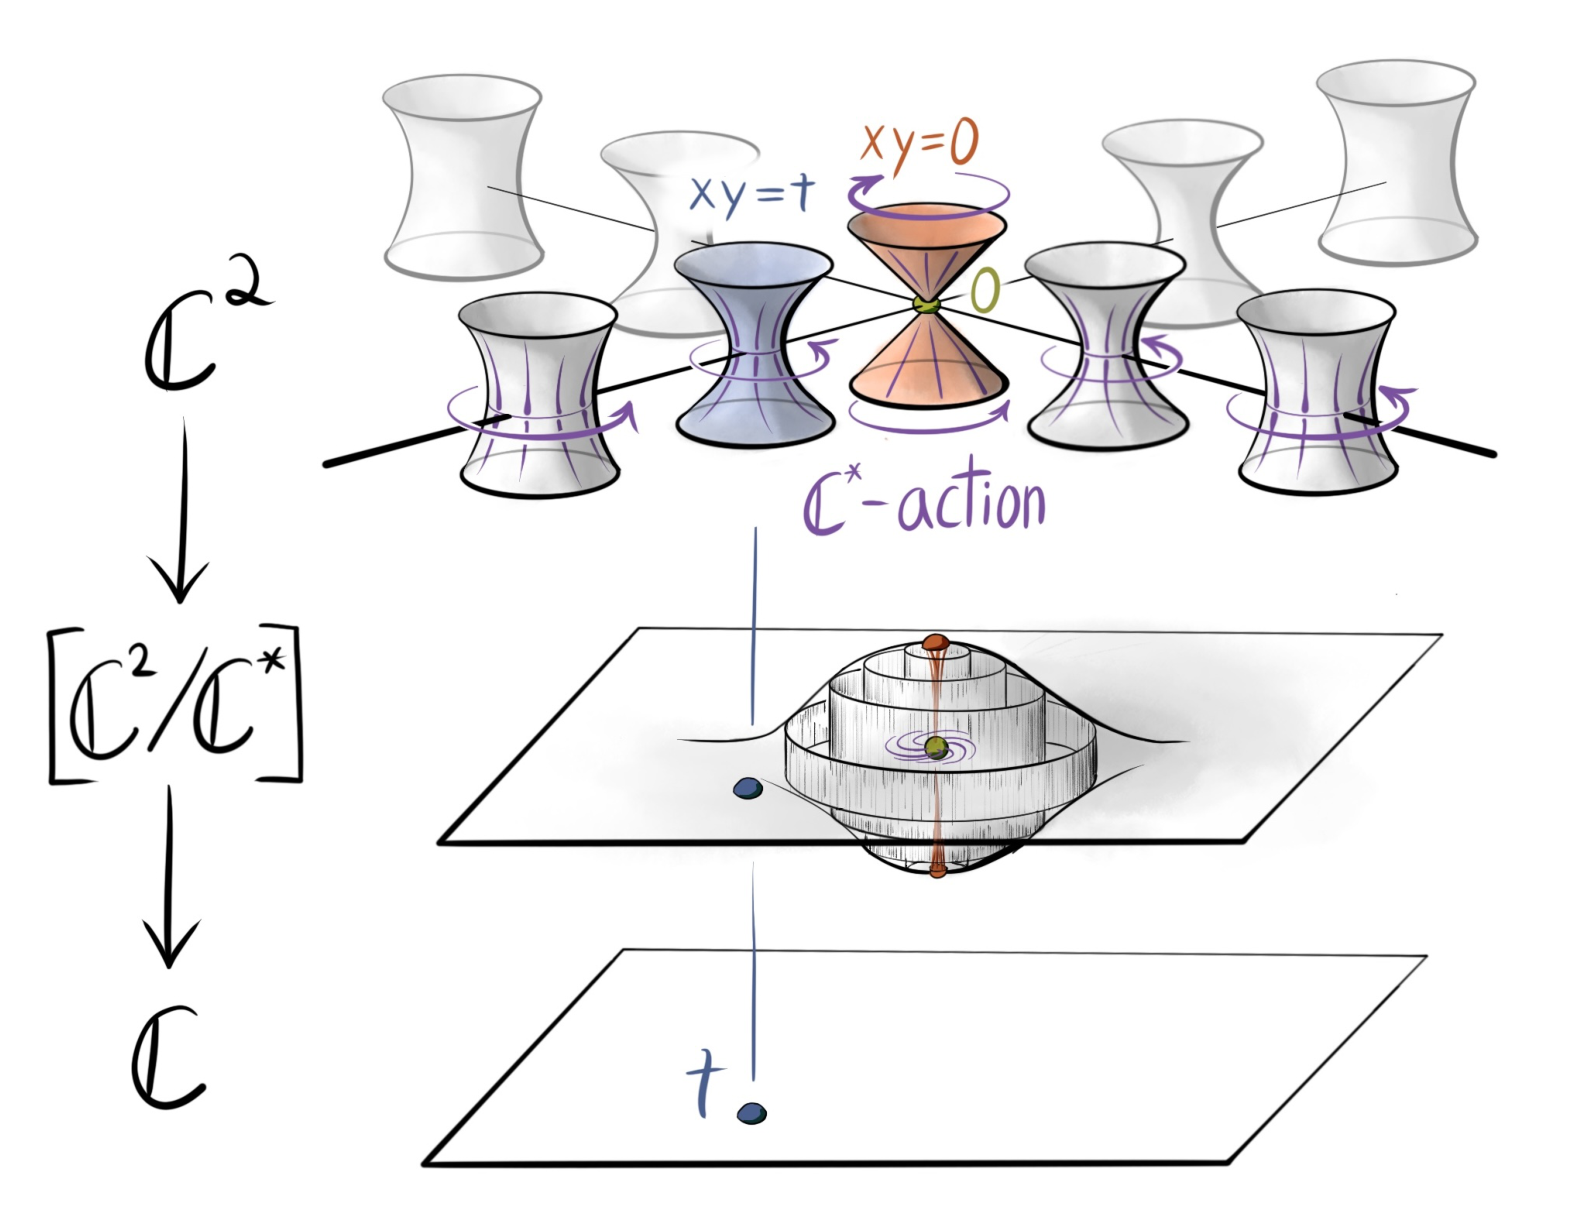
\includegraphics[width=.64\textwidth]{figures/fig-4.9.29.png}};
\begin{scope}[x={(art.south east)},y={(art.north west)}]
\fill[white] (0,0) rectangle (.205,1);
\node at (.105,.44) {\begin{tikzcd}[row sep=4.8em]
\mathbb C^2\arrow[d]\\
{[\mathbb C^2/\mathbb C^*]}\arrow[d]\\
\mathbb C
\end{tikzcd}};
\fill[white] (.50,.557) rectangle (.68,.628);
\node[text=violet,font=\small] at (.59,.593) {$\mathbb C^*$-作用};
\end{scope}
\end{tikzpicture}

\end{figure}
\end{example}
\begin{exercise}[表示叠]\label{src:4.9.30}
设 $G$ 是有限生成群, $n$ 是正整数.
\begin{enumerate}[(a)]
\item 定义 $\Gamma$ 的 $n$ 维表示叠 $\operatorname{Rep}_{\Gamma,n}$, 并证明它是代数叠.
\item 若 $\Gamma$ 是有 $\gamma$ 个生成元的自由群, 证明 $\operatorname{Rep}_{\Gamma,n}\cong[\operatorname{GL}_n^\gamma/\operatorname{GL}_n]$, 其中 $\operatorname{GL}_n$ 通过同时共轭作用.
\item 若 $\Gamma=\pi_1(\Sigma)$, 其中 $\Sigma$ 是亏格为 $g$ 的紧 Riemann 曲面, 证明
\[
\operatorname{Rep}_{\Gamma,n}\cong
\left[\left\{(\alpha_i,\beta_i)\in(\operatorname{GL}_n^2)^g\ \middle|\
\prod_{i=1}^g[\alpha_i,\beta_i]=1\right\}/\operatorname{GL}_n\right].
\]
\end{enumerate}
\end{exercise}
\begin{example}[环面叠]\label{src:4.9.31}
格 $L=\mathbb Z^n$ 上的扇 $\Sigma$ 定义环面簇 $X(\Sigma)$, 即带有 $\mathbb G_m^n$-作用且存在稳定子平凡的稠密轨道的正规分离簇; 见 \cite{Ful93}. 另一方面, \newterm{叠式扇}{stacky fan} 是二元组 $(\Sigma,\beta)$, 其中 $\Sigma$ 是格 $L$ 上的扇, $\beta:L\to N$ 是格之间的同态. 由于 $L,N$ 是格 (即有限生成自由 Abel 群), 它们的 $\mathbb Z$-线性对偶定义环面 $T_L:=D(L^\vee)$ 与 $T_N:=D(N^\vee)$ (例~\bookref{B.1.7}), 其中 $T_L$ 是环面簇 $X(\Sigma)$ 的环面. 映射 $\beta$ 诱导同态 $T_\beta:T_L\to T_N$, 自然地将 $\beta$ 与单参数子群格上的诱导映射等同. 于是可以定义 $G_\beta=\ker(T_\beta)$ 及\newterm{环面叠}{toric stack}
\[
\mathcal X(\Sigma,\beta):=[X(\Sigma)/G_\beta].
\]
与环面簇的作用类似, 环面叠提供了丰富的组合例子, 可以用来检验一般猜想. 见 \cite{FMN10,GS17}.
\end{example}
\begin{example}[Picard 概形与叠]\label{src:4.9.32}
设 $X$ 是代数闭域 $k$ 上的固有整概形. $X$ 的 Picard 函子与 Picard 叠定义为 $\Sch_{\text{ét}}$ 上的层 $\underline{\operatorname{Pic}}(X)$ 与叠 $\mathcal{P}ic(X)$:
\[
\begin{aligned}
\underline{\operatorname{Pic}}(X)&=\text{函子 }T\longmapsto\operatorname{Pic}(X_T)\text{ 的层化},\\
\mathcal{P}ic(X)(T)&=\{X_T\text{ 上的线丛 }L\text{ 组成的群胚}\}.
\end{aligned}
\]
$\mathcal{P}ic(X)$ 中的态射 $(T,L)\to(T',L')$ 由概形态射 $f:T\to T'$ 及同构 $\alpha:L\to f^*L'$ 给出. 层 $\underline{\operatorname{Pic}}(X)$ 可由射影概形表出, 而线丛的张量积赋予它群概形结构, 因而它是 Abel 簇. 此外, $\mathcal{P}ic(X)$ 是 $k$ 上的光滑代数叠. 忘掉自同构群的映射 $\mathcal{P}ic(X)\to\underline{\operatorname{Pic}}(X)$ 是带系 $\mathbb G_m$-gerbe 的一个例子. 见 \S\bookref{7.4.8-subsection}.
\end{example}
\begin{example}[向量丛叠]\label{src:4.9.33}
设 $K^\bullet:K^0\xrightarrow{d}K^1$ 是概形 $X$ 上的两项向量丛复形. \newterm{向量丛叠}{vector bundle stack} $\mathfrak C(K^\bullet)$, 有时称为\newterm{锥叠}{cone stack}, 并记为 $[K^1/K^0]$ 或 $[h^0/h^1]$, 定义为 $(\Sch/X)_{\text{ét}}$ 上的商叠
\[
\mathfrak C(K^\bullet)=[\mathbb A(K^{1,\vee})/\mathbb A(K^{0,\vee})],
\]
其中将 $\mathbb A(K^{0,\vee})$ 视为加法群概形, 作用 $\sigma:\mathbb A(K^{0,\vee})\times\mathbb A(K^{1,\vee})\to\mathbb A(K^{1,\vee})$ 定义为 $\sigma(x_0,x_1)=x_1+d(x_0)$. 当 $X=\Spec k$ 且 $k$ 是域时, $\mathfrak C(K^\bullet)(k)$ 是对象为 $\mathbb A(K^{1,\vee})(k)=K^1$ 的群胚, 态射 $v\to v'$ 是满足 $d(\alpha)=v-v'$ 的元素 $\alpha\in\mathbb A(K^{0,\vee})(k)=K^0$. 此外, $\mathfrak C(K^\bullet)$ 与平凡作用的商 $[\mathbb A(H^1(K^\bullet)^\vee)/\mathbb A(H^0(K^\bullet)^\vee)]$ 等同, 特别地, 群胚 $\mathfrak C(K^\bullet)(k)$ 等价于 $[H^1(K^\bullet)/H^0(K^\bullet)]$.

对一般的 $X$, $\mathfrak C(K^\bullet)\to X$ 在几何点 $\Spec k\to X$ 上的纤维为
\[
\mathfrak C(K^\bullet\otimes_{\mathcal O_X}k)\cong
[\mathbb A(H^1(K^\bullet\otimes_{\mathcal O_X}k)^\vee)/
\mathbb A(H^0(K^\bullet\otimes_{\mathcal O_X}k)^\vee)].
\]
若 $g:T\to X$ 是从仿射概形出发的态射, 则由于 $T$ 上的主 $\mathbb A(K^{0,\vee})$-丛的同构类与 $H^1(T,K^{0,\vee})=0$ 一一对应, 每个主丛均平凡. 因而
\[
\begin{aligned}
\mathfrak C(K^\bullet)(T)
&=[\mathbb A(K^{1,\vee})(T)/\mathbb A(K^{0,\vee})(T)]\\
&\cong[H^0(T,g^*K^1)/H^0(T,g^*K^0)],
\end{aligned}
\]
这里使用了双射
\begin{equation}\label{src:4.9.34}
\begin{aligned}
\mathbb A(K^{i,\vee})(T\xrightarrow{g}S)
&=\operatorname{Mor}_S(T,\mathbb A(K^{i,\vee}))\\
&=\operatorname{Hom}_{\mathcal O_S\text{-}\mathrm{alg}}
(\operatorname{Sym}^*K^{i,\vee},g_*\mathcal O_T)\\
&=\operatorname{Hom}_{\mathcal O_S}(K^{i,\vee},g_*\mathcal O_T)\\
&=H^0(S,K^i\otimes g_*\mathcal O_T)\\
&=H^0(S,g_*g^*K^i)\qquad\text{(投影公式)}\\
&=H^0(T,g^*K^i).
\end{aligned}
\end{equation}
由构造, $\mathfrak C(K^\bullet)\to X$ 是光滑态射, 对任意 $k$-值点 $\Spec k\to X$, 相对维数为 $h^1(K^\bullet\otimes_{\mathcal O_X}k)-h^0(K^\bullet\otimes_{\mathcal O_X}k)$.
\end{example}
\begin{exercise}\label{src:4.9.35}
证明概形 $X$ 上的两项复形之间的拟同构 $K^\bullet\to L^\bullet$ 诱导向量丛叠之间的同构 $\mathfrak C(K^\bullet)\xrightarrow{\sim}\mathfrak C(L^\bullet)$.
\end{exercise}
上面的习题说明, 对振幅在 $[0,1]$ 内的复形 $K^\bullet\in D^b(X)$, 向量丛叠 $\mathfrak C(K^\bullet)$ 是良定义的. 我们将在命题~\bookref{9.2.13} 中用此构造描述 $C\times S$ 上向量丛 $F_1,F_2$ 的扩张叠 $\mathfrak C(Rp_{2,*}\mathcal H om_{\mathcal O_{C\times S}}(F_1,F_2))\to S$, 其中 $C$ 是\mbox{光滑曲线}. 对于 syntomic 态射 $X\to Y$, $L_{X/Y}$ 是振幅在 $[-1,0]$ 内的完美复形, 可以考虑向量丛叠 $\mathfrak C(L_{X/Y}^\vee)$, 它在 \cite{BF97} 中内蕴法锥的定义中起作用.

\subsection{极端不分离的例子}\label{src:4.9.4-subsection}
下面的例子常常提供反例: 某些性质对具有分离且拟紧对角线的代数叠成立, 但在一般情形下失效. 例如, 若 Deligne--Mumford 叠的对角线拟紧且分离, 则它拟仿射 (推论~\bookref{5.5.8}), 特别地可由概形表出; 下面的例子说明拟紧性与分离性两个假设都不可少.
\begin{example}[对角线不拟紧的 Deligne--Mumford 叠]\label{src:4.9.36}
设 $\underline{\mathbb Z}$ 表示 $\Spec\mathbb Z$ 上与抽象离散群 $\mathbb Z$ 对应的常群概形. 分类叠 $B\underline{\mathbb Z}$ 是零维光滑代数叠, 其对角线不拟紧. 特别地, $B\underline{\mathbb Z}$ 不拟分离.

在特征为零的域 $k$ 上, 令 $\mathbb Z$ 作用于 $\mathbb A^1$, 对 $x\in\mathbb A^1$ 与 $n\in\mathbb Z$, 作用为 $n\cdot x=x+n$. 商 $G:=\mathbb A^1/\mathbb Z$ 是拟紧且局部 Noether 的群代数空间, 其对角线不拟紧, 且它不是概形. 域 $k$ 上每个局部有限型的拟分离群代数空间都是概形 (定理~\bookref{5.5.28}), 而此例说明拟分离性假设不可少.

分类叠 $BG$ 是 Deligne--Mumford 叠, 其对角线 $\Delta_{BG}$ 拟紧, 但二重对角线 $\Delta_{\Delta_{BG}}$ 不拟紧; 特别地, $BG$ 不拟分离. 此外, $BG$ 的对角线不可由概形表出.

类似地, 可以考虑代数空间商 $\mathbb A^1_{\mathbb C}/\mathbb Z^2$, 其中 $(a,b)\cdot x=x+a+ib$. 虽然此作用的解析商 $\mathbb C/\mathbb Z^2$ 是 $\mathbb C$ 上的椭圆曲线, 但代数空间商不拟分离, 也不是概形.
\end{example}
\begin{exercise}\label{src:4.9.37}
设 $G=\mathbb A^1/\mathbb Z$.
\begin{enumerate}[(a)]
\item 证明 $G$ 不是概形.
\item 证明一般点 $\Spec k(x)\to\mathbb A^1\to X$ 在 $\mathbb Z$-作用下不变, 且复合 $\Spec k(x)\to G$ 不能经过从某个域 $L$ 出发的单态射 $\Spec L\to G$ 分解, 即 $G$ 的一般点没有剩余域.
\end{enumerate}
\end{exercise}
\begin{example}[对角线不分离的 Deligne--Mumford 叠]\label{src:4.9.38}
不分离仿射直线 $Q:=\mathbb A^1\cup_{\mathbb A^1\setminus0}\mathbb A^1$ 是 $\mathbb A^1$ 上的群概形, 除原点上外每个纤维都平凡. 分类叠 $BQ$ 是对角线不分离的 Deligne--Mumford 叠.

下面给出产生类似例子的构造. 设 $G\to S$ 是有限平展群概形. 若 $H\subseteq G$ 是 $S$ 上的子群概形, 则 $G/H$ 分离当且仅当 $H\subset G$ 闭. 若 $H$ 在 $G$ 中正规, 则 $G/H\to S$ 是群代数空间. 例如, 取 $G=\mathbb Z/2\times\mathbb A^1\to\mathbb A^1$ 及子群 $H=G\setminus\{-1,0\}$, 则商 $Q=G/H$ 是 $\mathbb A^1$ 上的不分离仿射直线.

类似地, 考虑 $\mathbb Q$ 上的 $\mu_{3,\mathbb Q}=\Spec\mathbb Q\amalg G'$, 其中 $G'=\Spec\mathbb Q[x]/(x^2+x+1)$ 是非单位分支, 并令 $G=\mu_{3,\mathbb Q}\times\mathbb A^1_{\mathbb Q}$. 则 $Q=(\mu_{3,\mathbb Q}\times\mathbb A^1_{\mathbb Q})/H$ 是 $\mathbb A^1_{\mathbb Q}$ 上的不分离平展群代数空间, 且不是概形. 它不是概形的原因与习题~\bookref{4.9.7} 类似: $Q\to\mathbb A^1$ 是群概形
\[
\mathbb A^1_{\mathbb Q}\cup_{\mathbb A^1_{\mathbb Q}\setminus0}
\mathbb A^1_{\mathbb Q}\cup_{\mathbb A^1_{\mathbb Q}\setminus0}\mathbb A^1_{\mathbb Q}
\]
的一个形式, 该群概形除原点上的纤维为 $\mathbb Z/2$ 外均平凡. 若 $Q_0$ 中的非单位点包含于一个仿射开集, 则其在 $\mathbb A^1_{\mathbb Q[x]/(x^2+x+1)}\to\mathbb A^1_{\mathbb Q}$ 下的原像是包含其中两个原点的仿射开集, 矛盾.

此时, $BQ$ 是拟紧且拟分离的 Deligne--Mumford 叠 (即 $BG$, 一重对角线 $\Delta_{BG}$ 与二重对角线 $\Delta_{\Delta_{BG}}$ 都拟紧), 但其对角线不分离且不可由概形表出.
\end{example}
虽然模理论中出现的绝大多数代数叠都具有分离对角线, 但也有少数例外, 例如对数结构叠 $\operatorname{Log}_{\mathrm{alg}}$ \cite{Ols03}.
\par\clearpage
\endgroup

% Source printed p. 165 / PDF p. 173.
\chapter[Deligne--Mumford 叠的几何]{\texorpdfstring{\raggedright Deligne--Mumford\\叠的几何}{Deligne--Mumford 叠的几何}}\label{src:5}
\begin{epigraph}
几何是数学中的香菜.
\epigraphauthor{Jordan Ellenberg}
\end{epigraph}

% Source printed pp. 165-175 / PDF pp. 173-183.
\section{拟凝聚层与上同调}\label{src:5.1}
\begin{epigraph}
若不受牢固的人际关系制约, 以抽象观念为指导是件危险的事.
\epigraphauthor{Paul Feyerabend, \textit{科学的暴政}}
\end{epigraph}

\subsection{层}\label{src:5.1.1-subsection}
Deligne--Mumford 叠的小平展景可类似于概形的小平展景定义 (例~\bookref{3.2.4}).
\begin{definition}\label{src:5.1.1}
Deligne--Mumford 叠 $\mathcal X$ 的\newterm{小平展景}{small étale site} 是由 $\mathcal X$ 上的平展概形组成的范畴 $\mathcal X_{\text{ét}}$. 一个 $\mathcal X$-概形 $U$ 的覆盖是 $\mathcal X$ 上的一族平展态射 $\{U_i\to U\}$, 使得 $\coprod_i U_i\to U$ 满射.
\end{definition}
于是可以讨论 $\mathcal X_{\text{ét}}$ 上的 Abel 群层及其态射. 以 $\mathsf{Ab}(\mathcal X_{\text{ét}})$ 记 $\mathcal X_{\text{ét}}$ 上 Abel 层的范畴. 对 $\mathcal X_{\text{ét}}$ 上的 Abel 层 $F$, 以 $F(U\to\mathcal X)$ 记它在平展 $\mathcal X$-概形 $U$ 上的截面.
\begin{example}[结构层]\label{src:5.1.2}
Deligne--Mumford 叠上的\newterm{结构层}{structure sheaf} $\mathcal O_{\mathcal X}$ 在平展 $\mathcal X$-概形 $U$ 上定义为 $\mathcal O_{\mathcal X}(U\to\mathcal X)=\Gamma(U,\mathcal O_U)$.
\end{example}
\begin{example}[微分]\label{src:5.1.3}
若 $\mathcal X$ 是概形 $S$ 上的 Deligne--Mumford 叠, 则\newterm{相对微分层}{relative sheaf of differentials} $\Omega_{\mathcal X/S}$ 定义为 $\Omega_{\mathcal X/S}(U\to\mathcal X)=\Gamma(U,\Omega_{U/S})$.
\end{example}
\begin{example}[Hodge 丛]\label{src:5.1.4}
在 $\mathcal M_g$ ($g\geq2$) 上如下定义层 $\mathcal H$: 对由光滑曲线族 $\mathcal C\to U$ 分类的平展态射 $U\to\mathcal M_g$, 置 $\mathcal H(U\to\mathcal M_g)=\Gamma(\mathcal C,\Omega_{\mathcal C/U})$. 稍后将看到 $\mathcal H$ 是凝聚 $\mathcal O_{\mathcal M_g}$-模, 事实上是秩 $g$ 的\newterm{Hodge 丛}{Hodge bundle}.
\end{example}
\begin{exercise}[简单]\label{src:5.1.5}
若 $k$ 是代数闭域, 证明由 $F\mapsto F(\Spec k)$ 定义的函子 $\mathsf{Ab}((\Spec k)_{\text{ét}})\to\mathsf{Ab}$ 是范畴等价.
\end{exercise}
虽然 $\mathcal X_{\text{ét}}$ 上的层 $F$ 的截面只在平展 $\mathcal X$-概形上定义, 但可如下将定义延伸到 $\mathcal X$ 上的平展 Deligne--Mumford 叠 $\mathcal U$: 选取来自概形的平展呈示 $U\to\mathcal U$ 和 $R\to U\times_{\mathcal U}U$, 并定义
\[
F(\mathcal U\to\mathcal X):=\operatorname{Eq}\bigl(F(U\to\mathcal X)\rightrightarrows F(R\to\mathcal X)\bigr).
\]
可以检验这与呈示的选择无关. 特别地, 可以讨论整体截面
\[
\Gamma(\mathcal X,F):=F(\mathcal X\xrightarrow{\mathrm{id}}\mathcal X).
\]
\begin{exercise}[简单]\label{src:5.1.6}
若 $F$ 是 Deligne--Mumford 叠 $\mathcal X$ 上的 Abel 层, 证明 $\Gamma(\mathcal X,F)=\operatorname{Hom}_{\mathsf{Ab}(\mathcal X_{\text{ét}})}(\underline{\mathbb Z},F)$, 其中 $\underline{\mathbb Z}$ 是常值层.
\end{exercise}
给定 Deligne--Mumford 叠的态射 $f:\mathcal X\to\mathcal Y$, 有函子
\[
\begin{tikzcd}
\mathsf{Ab}(\mathcal X_{\text{ét}})\arrow[r,shift left,"f_*"]&\mathsf{Ab}(\mathcal Y_{\text{ét}})\arrow[l,shift left,"f^{-1}"] .
\end{tikzcd}
\]
其中\newterm{推前}{pushforward} 定义为 $f_*F(V\to\mathcal Y):=F(\mathcal X\times_{\mathcal Y}V\to\mathcal X)$, 而\newterm{逆像}{inverse image} $f^{-1}G$ 是预层
\[
(U\to\mathcal X)\longmapsto\mathop{\mathrm{colim}}_{(V\to\mathcal Y,\,U\to\mathcal X\times_{\mathcal Y}V)}G(V\to\mathcal Y)
\]
的层化. 此处余极限遍历平展态射对 $V\to\mathcal Y$ 与 $U\to\mathcal X\times_{\mathcal Y}V$, 即交换图
\[
\begin{tikzcd}
U\arrow[r]\arrow[d,"\text{平展}"']&V\arrow[d,"\text{平展}"]\\
\mathcal X\arrow[r]&\mathcal Y.
\end{tikzcd}
\]
\begin{exercise}[简单]\label{src:5.1.7}
证明若 $f:\mathcal X\to\mathcal Y$ 是 Deligne--Mumford 叠的平展态射, $G$ 是 $\mathcal Y_{\text{ét}}$ 上的层, 则 $f^{-1}G=G|_{\mathcal X}$ 是 $G$ 在 $\mathcal X_{\text{ét}}$ 上的限制, 即层 $(U\to\mathcal X)\mapsto G(U\to\mathcal X\to\mathcal Y)$. 特别地, 证明 $f^{-1}\mathcal O_{\mathcal Y}=\mathcal O_{\mathcal X}$.
\end{exercise}
\begin{exercise}[简单]\label{src:5.1.8}
设 $X$ 是概形, $x\in X$.
\begin{enumerate}[(a)]
\item 记 $i_x:\Spec\kappa(x)\to X$, 证明 $i_x^{-1}\mathcal O_X$ 的整体截面是 $\mathcal O_{X,x}$ 的 Hensel 化 $\mathcal O^h_{X,x}$.
\item 记 $i_{\overline x}:\Spec\overline{\kappa(x)}\to X$, 证明 $i_{\overline x}^{-1}$ 可与 $\mathcal O_{X,x}$ 的严格 Hensel 化 $\mathcal O^{\mathrm{sh}}_{X,x}$ 等同.
\end{enumerate}
关于 (严格) Hensel 化的背景, 见 \S\bookref{B.5.3-subsection}.
\end{exercise}
\begin{exercise}\label{src:5.1.9}
设 $k$ 是域, $k^{\mathrm{sep}}$ 是可分闭包, $G:=\operatorname{Gal}(k^{\mathrm{sep}}/k)$ 是赋予 profinite 拓扑的 Galois 群.
\begin{enumerate}[(a)]
\item 证明协变函子 $F:\{\text{平展 $k$-代数}\}\to\mathsf{Ab}$ 定义 $(\Spec k)_{\text{ét}}$ 上的 Abel 群层, 当且仅当对每个有限平展 $k$-代数族 $\{A_i\}$ 有 $F(\prod_i A_i)=\bigoplus_i F(A_i)$, 且对 $k$ 的有限可分域扩张之间的每个有限 Galois 扩张 $L/K$ 有 $F(K)=F(L)^{\operatorname{Gal}(L/K)}$.
\item 证明 $(\Spec k)_{\text{ét}}$ 上层的范畴等价于离散 $G$-模的范畴, 即带连续 $G$-作用的 Abel 群的范畴.

\textit{提示:} 给定 $F$, 定义离散 $G$-模 $M_F:=\mathrm{colim}_{k'/k}F(k')$, 其中余极限遍历有限可分域扩张. 反之, 给定 $M$, 证明有限域扩张上的函子 $k'\mapsto M^{\operatorname{Gal}(k^{\mathrm{sep}}/k')}$ 延伸为 $(\Spec k)_{\text{ét}}$ 上的层 $F_M$. 证明 $M\mapsto M_F$ 与 $M\mapsto F_M$ 是互逆函子.
\end{enumerate}
\end{exercise}
\newpage
\begin{exercise}\label{src:5.1.10}
设 $\mathcal X$ 是 Deligne--Mumford 叠, $x:\Spec k\to\mathcal X$ 是几何点 (即 $k$ 是代数闭域). 定义 $\mathcal X_{\text{ét}}$ 上的 Abel 层 $F$ 在 $x$ 处的\newterm{茎}{stalk} 为 $F_x:=x^{-1}F$.
\begin{enumerate}[(a)]
\item 证明由 $F\mapsto F_x$ 定义的函子 $\mathsf{Ab}(\mathcal X_{\text{ét}})\to\mathsf{Ab}$ 正合.
\item 证明 $\mathcal X_{\text{ét}}$ 上的 Abel 层序列正合, 当且仅当对每个几何点, 所诱导的茎序列正合.
\item 证明对 Deligne--Mumford 叠的态射 $f:\mathcal X\to\mathcal Y$, $f^{-1}$ 正合.
\end{enumerate}
\end{exercise}
\begin{exercise}[细节]\label{src:5.1.11}
证明 $f^{-1}$ 是 $f_*$ 的左伴随.
\end{exercise}
\begin{exercise}[技术性]\label{src:5.1.12}
若 $\mathcal X$ 是 Deligne--Mumford 叠, 另定义景 $\mathcal X_{\text{ét}'}$ 为 $\mathcal X$ 上平展代数空间的范畴, 覆盖取平展覆盖. 证明 $\mathcal X_{\text{ét}}$ 与 $\mathcal X_{\text{ét}'}$ 上层的范畴等价.
\end{exercise}

\subsection{\texorpdfstring{$\mathcal O_{\mathcal X}$}{OX}-模}\label{src:5.1.2-subsection}
结构层 $\mathcal O_{\mathcal X}$ 是 $\mathsf{Ab}(\mathcal X_{\text{ét}})$ 中的环对象, $\mathcal O_{\mathcal X}$-模定义为 $\mathcal O_{\mathcal X}$ 上的模对象.
\begin{definition}\label{src:5.1.13}
若 $\mathcal X$ 是 Deligne--Mumford 叠, 则\newterm{$\mathcal O_{\mathcal X}$-模层}{sheaf of $\mathcal O_{\mathcal X}$-modules} (或简称 $\mathcal O_{\mathcal X}$-模) 是 $\mathcal X_{\text{ét}}$ 上的层 $F$, 它是层范畴中 $\mathcal O_{\mathcal X}$ 的模对象, 即对每个平展 $\mathcal X$-概形 $U$, $F(U\to\mathcal X)$ 是 $\mathcal O_{\mathcal X}(U\to\mathcal X)=\Gamma(U,\mathcal O_U)$ 上的模, 且模结构与沿平展 $\mathcal X$-概形之间态射 $V\to U$ 的限制相容.
\end{definition}
以 $\Mod(\mathcal O_{\mathcal X})$ 记 $\mathcal O_{\mathcal X}$-模的范畴. 给定两个 $\mathcal O_{\mathcal X}$-模 $F,G$, 可将\newterm{张量积}{tensor product} $F\otimes G:=F\otimes_{\mathcal O_{\mathcal X}}G$ 定义为由 $(U\to\mathcal X)\mapsto F(U\to\mathcal X)\otimes_{\mathcal O_{\mathcal X}(U\to\mathcal X)}G(U\to\mathcal X)$ 给出的 $\mathcal O_{\mathcal X}$-模的层化. 对来自概形的平展态射 $f:U\to\mathcal X$, \newterm{Hom 层}{Hom sheaf} $\mathcal H\!om_{\mathcal O_{\mathcal X}}(F,G)$ 在其上的截面为 $\operatorname{Hom}_{\mathcal O_U}(F|_U,G|_U)$, 其中 $F|_U=f^{-1}F$ 表示 $F$ 在 $U_{\text{ét}}$ 上的限制.
\begin{exercise}[简单]\label{src:5.1.14}
若 $F$ 是 $\mathcal O_{\mathcal X}$-模, 证明 $\Gamma(\mathcal X,F)=\operatorname{Hom}_{\mathcal O_{\mathcal X}}(\mathcal O_{\mathcal X},F)$.
\end{exercise}
给定 Deligne--Mumford 叠的态射 $f:\mathcal X\to\mathcal Y$, 有函子
\[
\begin{tikzcd}
\Mod(\mathcal O_{\mathcal X})\arrow[r,shift left,"f_*"]&\Mod(\mathcal O_{\mathcal Y})\arrow[l,shift left,"f^*"] .
\end{tikzcd}
\]
其中对 $\mathcal O_{\mathcal X}$-模 $F$, $f_*F$ 是作为层的推前, 并自然成为 $\mathcal O_{\mathcal Y}$-模. 对 $\mathcal O_{\mathcal Y}$-模 $G$, 由于在 $\mathcal X_{\text{ét}}$ 上有环层态射 $f^{-1}\mathcal O_{\mathcal Y}\to\mathcal O_{\mathcal X}$, 且 $f^{-1}G$ 是 $f^{-1}\mathcal O_{\mathcal Y}$-模, 可以将\newterm{拉回}{pullback} 定义为 $\mathcal O_{\mathcal X}$-模
\[
f^*G:=f^{-1}G\otimes_{f^{-1}\mathcal O_{\mathcal Y}}\mathcal O_{\mathcal X}.
\]
若 $f$ 平展, 则 $f^*G=f^{-1}G=G|_{\mathcal X}$, 因为 $f^{-1}\mathcal O_{\mathcal Y}=\mathcal O_{\mathcal X}$ (习题~\bookref{5.1.7}).
\begin{exercise}[细节]\label{src:5.1.15}
证明 $f^*$ 是 $f_*$ 的左伴随.
\end{exercise}
\begin{exercise}[细节]\label{src:5.1.16}
证明 $\Mod(\mathcal O_{\mathcal X})$ 是 Abel 范畴.
\end{exercise}

\subsection{拟凝聚层}\label{src:5.1.3-subsection}
设 $F$ 是 Deligne--Mumford 叠 $\mathcal X$ 上的 $\mathcal O_{\mathcal X}$-模. 对平展 $\mathcal X$-概形 $U$, 有 $F$ 在 $U$ 的小平展景 $U_{\text{ét}}$ 上的限制 $F|_{U_{\text{ét}}}$, 以及进一步在 $U$ 的 Zariski 拓扑上的限制 $F|_{U_{\mathrm{Zar}}}$. 注意当 $X$ 是概形时, $\mathcal O_X$ 既可指 $X_{\text{ét}}$ 上的结构层, 也可指 $X_{\mathrm{Zar}}$ 上的结构层; 可能混淆时, 分别写作 $\mathcal O_{X_{\text{ét}}}$ 和 $\mathcal O_{X_{\mathrm{Zar}}}$.
\begin{definition}\label{src:5.1.17}
设 $\mathcal X$ 是 Deligne--Mumford 叠. 一个 $\mathcal O_{\mathcal X}$-模 $F$ 称为\newterm{拟凝聚的}{quasi-coherent}, 若
\begin{enumerate}[(1)]
\item 对每个平展 $\mathcal X$-概形 $U$, 限制 $F|_{U_{\mathrm{Zar}}}$ 是拟凝聚 $\mathcal O_{U_{\mathrm{Zar}}}$-模, 且
\item 对平展 $\mathcal X$-概形之间的每个平展态射 $f:U\to V$, 自然态射 $f^*(F|_{V_{\mathrm{Zar}}})\to F|_{U_{\mathrm{Zar}}}$ 是同构.
\end{enumerate}
$\mathcal X$ 上的拟凝聚 $\mathcal O_{\mathcal X}$-模 $F$ 称为\newterm{向量丛}{vector bundle} (分别为秩 $r$ 的向量丛, 线丛), 若对来自概形的每个平展态射 $U\to\mathcal X$, $F|_{U_{\mathrm{Zar}}}$ 都具有相应性质. 若此外 $\mathcal X$ 局部 Noether, 则称 $F$ 为\newterm{凝聚的}{coherent}, 若对每个平展态射 $U\to\mathcal X$, $F|_{U_{\mathrm{Zar}}}$ 凝聚.
\end{definition}
以 $\QCoh(\mathcal X)$ 和 $\operatorname{Coh}(\mathcal X)$ (在 Noether 情形) 分别记拟凝聚层和凝聚层的范畴. 稍后将看到当 $\mathcal X$ 是概形时, 这与通常的定义一致; 先给出几个例子.
\begin{example}\label{src:5.1.18}
结构层 $\mathcal O_{\mathcal X}$ 拟凝聚. 它是线丛, 当 $\mathcal X$ 局部 Noether 时凝聚.
\end{example}
\begin{example}\label{src:5.1.19}
对概形 $S$ 上的 Deligne--Mumford 叠 $\mathcal X$, 例~\bookref{5.1.3} 的相对微分层 $\Omega_{\mathcal X/S}$ 拟凝聚, 因为对平展 $\mathcal X$-概形之间的平展态射 $f:U\to V$, $f^*\Omega_{V/S}\to\Omega_{U/S}$ 是同构. 当 $\mathcal X\to S$ 光滑时, 它是向量丛.
\end{example}
\begin{example}\label{src:5.1.20}
对 $\mathcal M_g$ ($g\geq2$), 例~\bookref{5.1.4} 的 Hodge 丛 $\mathcal H$ 是秩 $g$ 的向量丛. 这由命题~\bookref{6.1.16}(2) 推出: 对应于 $\mathcal M_g$-概形 $V$ 的亏格 $g$ 光滑曲线族 $\pi:\mathcal C\to V$, 构造 $\pi_*\Omega_{\mathcal C/V}$ 与沿映射 $f:U\to V$ 的基变换交换, 即
\[
f^*(\pi_*\Omega_{\mathcal C/V})\xrightarrow{\sim}\pi_{U,*}\Omega_{\mathcal C_U/U}
\]
(这说明 $\mathcal H$ 拟凝聚); 此外 $\pi_*\Omega_{\mathcal C/V}$ 是 $V$ 上秩 $g$ 的向量丛 (这说明 $\mathcal H$ 是秩 $g$ 的向量丛).
\end{example}
\begin{example}\label{src:5.1.21}
若 $G$ 是视作域 $k$ 上群概形的有限抽象群, 则 $BG$ 上的拟凝聚层对应于 $G$ 的表示 $V$. 若 $G$ 作用于仿射 $k$-概形 $\Spec A$, 则 $[\Spec A/G]$ 上的拟凝聚层由一个 $A$-模 $M$ 及群同态 $G\to\operatorname{End}_A(M)$ 给出. 这些描述由习题~\bookref{5.1.24}(b) 推出.
\end{example}
\begin{exercise}[等价性 I]\label{src:5.1.22}
设 $X$ 是概形.
\begin{enumerate}[(a)]
\item 证明对 $\mathcal O_{X_{\text{ét}}}$-模 $F$, 以下条件等价:
\begin{enumerate}[(i)]
\item $F$ 按定义~\bookref{5.1.17} 拟凝聚.
\item 存在拟凝聚 $\mathcal O_{X_{\mathrm{Zar}}}$-模 $F'$ 及同构 $F\cong\alpha^*F'$, 其中 $\alpha^*:\Mod(\mathcal O_{X_{\mathrm{Zar}}})\to\Mod(\mathcal O_{X_{\text{ét}}})$ 是将 $\mathcal O_{X_{\mathrm{Zar}}}$-模 $F'$ 送到 $\mathcal O_{X_{\text{ét}}}$-模 $\alpha^*F'$ 的函子, 后者定义为 $\alpha^*F'(U\xrightarrow{g}X)=\Gamma(U,g^*F')$.
\item $F$ 是赋环景 $(X_{\text{ét}},\mathcal O_{X_{\text{ét}}})$ 中的拟凝聚模对象, 这里使用一般赋环景 $(\mathcal S,\mathcal O)$ 中的定义~\cite[Tag 03DL]{SP}: $\mathcal O$-模 $F$ 称为拟凝聚的, 若对每个对象 $U\in\mathcal S$, 存在覆盖 $\{U_i\to U\}$, 使得它在限制景 $\mathcal S/U_i$ 上的限制 $F|_{U_i}$ 有自由呈示
\[
\mathcal O_{U_i}^{\oplus J}\longrightarrow\mathcal O_{U_i}^{\oplus I}\longrightarrow F|_{U_i}\longrightarrow0.
\]
\end{enumerate}
\textit{提示:} 证明 (iii) 蕴含其余条件时, 使用拟凝聚层的 fpqc 下降 (\bookref{3.1.4}) 构造拟凝聚层.
\item 证明 $\alpha^*$ 限制为范畴等价 $\QCoh(X_{\mathrm{Zar}})\to\QCoh(X_{\text{ét}})$.

\textit{提示:} 证明将 $\mathcal O_{X_{\text{ét}}}$-模限制到 Zariski 拓扑的运算 $F|_{X_{\mathrm{Zar}}}$ 定义了 $\alpha^*$ 的左伴随 $\alpha_*$. 利用伴随关系, 以及对拟凝聚 $\mathcal O_{X_{\mathrm{Zar}}}$-模 $F$ 的等同 $\alpha_*\alpha^*F\cong F$, 证明 $\alpha^*$ 在拟凝聚层上完全忠实.
\end{enumerate}
\end{exercise}
\begin{exercise}\label{src:5.1.23}
给出一个概形 $X$ 及非拟凝聚的 $\mathcal O_{X_{\text{ét}}}$-模 $F$, 使得 $F|_{X_{\mathrm{Zar}}}$ 拟凝聚.
\end{exercise}
这说明定义~\bookref{5.1.17} 中条件 (2) 的必要性.
\begin{exercise}[等价性 II]\label{src:5.1.24}
设 $\mathcal X$ 是 Deligne--Mumford 叠.
\begin{enumerate}[(a)]
\item 证明对 $\mathcal O_{\mathcal X_{\text{ét}}}$-模 $F$, 以下条件等价:
\begin{enumerate}[(i)]
\item $F$ 按定义~\bookref{5.1.17} 拟凝聚.
\item 存在来自概形的平展呈示 $U\to\mathcal X$, 使得 $F|_{U_{\text{ét}}}$ 拟凝聚.
\item $F$ 是赋环景 $(\mathcal X_{\text{ét}},\mathcal O_{\mathcal X_{\text{ét}}})$ 中的拟凝聚模层.
\end{enumerate}
\item 设 $U\to\mathcal X$ 是平展呈示, 置 $R=U\times_{\mathcal X}U$. 证明 $\mathcal X$ 上的拟凝聚层范畴等价于对 $(G,\alpha)$ 的范畴, 其中 $G$ 是 $U$ 上的拟凝聚层, $\alpha:p_1^*G\xrightarrow{\sim}p_2^*G$ 是 $R:=U\times_{\mathcal X}U$ 上满足上循环条件 $p_{23}^*\alpha\circ p_{12}^*\alpha=p_{13}^*\alpha$ 的同构.
\item 证明 $\mathcal X$ 上的拟凝聚层等价于如下数据: 对 $\mathcal X$ 上的每个概形 $U$, 给定拟凝聚层 $F_U$, 并对 $\mathcal X$ 上概形之间的每个映射 $f:U\to V$, 给定相容的同构 $f^*F_V\to F_U$.
\end{enumerate}
\end{exercise}
习题~\bookref{5.1.24}(c) 给出了理解模叠上拟凝聚层的一种方便且函子性的方式. 例如, $\mathcal M_g$ 上的 Hodge 丛可视为对每个光滑曲线族 $\pi:\mathcal C\to S$ 给定层 $\pi_*\Omega_{\mathcal C/S}$ 的数据.
\begin{exercise}[等价性 III]\label{src:5.1.25}
给定 Deligne--Mumford 叠 $\mathcal X$, 类似于 \S\bookref{3.2.2-subsection} 中概形上的定义, 定义大平展景 $(\Sch/\mathcal X)_{\text{ét}}$, 大 fppf 景 $(\Sch/\mathcal X)_{\mathrm{fppf}}$ 和光滑平展景 $\mathcal X_{\text{lis-ét}}$. 每个景都有结构层 $\mathcal O$, 称 $\mathcal O$-模拟凝聚, 若它作为赋环景中的模层拟凝聚. 证明存在等价
\[
\begin{aligned}
\QCoh(\mathcal X_{\text{ét}})&\xrightarrow{\sim}\QCoh(\mathcal X_{\text{lis-ét}})\xrightarrow{\sim}\QCoh((\Sch/\mathcal X)_{\text{ét}})\\
&\xrightarrow{\sim}\QCoh((\Sch/\mathcal X)_{\mathrm{fppf}}),
\end{aligned}
\]
其定义类似于习题~\bookref{5.1.22} 中概形 $X$ 上的等价 $\QCoh(X_{\mathrm{Zar}})\xrightarrow{\sim}\QCoh(X_{\text{ét}})$.
\end{exercise}

\subsection{推前与拉回}\label{src:5.1.4-subsection}
\begin{exercise}[推前--拉回伴随]\label{src:5.1.26}
设 $f:\mathcal X\to\mathcal Y$ 是 Deligne--Mumford 叠的态射.
\begin{enumerate}[(a)]
\item 证明 $f^*$ 保持拟凝聚性.
\item 若 $f$ 拟紧且拟分离, 证明 $f_*$ 保持拟凝聚性, 并推出
\[
\begin{tikzcd}
\QCoh(\mathcal X)\arrow[r,shift left,"f_*"]&\QCoh(\mathcal Y)\arrow[l,shift left,"f^*"]
\end{tikzcd}
\]
是伴随函子 ($f_*$ 为右伴随).
\end{enumerate}
\end{exercise}
\begin{exercise}[有益的练习]\label{src:5.1.27}
设 $G$ 是有限群, $k$ 是域.
\begin{enumerate}[(a)]
\item 考虑 $G$ 的表示 $V$, 并利用例~\bookref{5.1.21} 将它也视作 $BG$ 上的拟凝聚层. 对复合 $\Spec k\xrightarrow{p}BG\xrightarrow{\pi}\Spec k$, 证明 $\pi_*V=V^G$, 其中 $V^G$ 是 $G$-不变量子空间; 而 $p^*V=V$, 即忘掉 $G$-作用. 此外, 对 $k$-向量空间 $W$, 证明 $\pi^*W=W$, 赋予平凡 $G$-作用, 且 $p_*W=W\otimes p_*k$, 其中 $p_*k$ 是正则表示 $\Gamma(G,\mathcal O_G)$.
\item 给定 $G$ 在仿射 $k$-概形 $\Spec A$ 上的作用, 考虑图
\[
\begin{tikzcd}
\Spec A\arrow[r,"p"]&{[\Spec A/G]}\arrow[r,"\pi"]\arrow[d,"q"]&\Spec A^G\\
&BG&
\end{tikzcd}
\]
并回顾例~\bookref{5.1.21}, $[\Spec A/G]$ 上的拟凝聚层是带群同态 $G\to\operatorname{End}_A(M)$ 的 $A$-模 $M$. 显式描述拟凝聚层上的函子 $p_*,p^*,\pi_*,\pi^*,q_*,q^*$.
\end{enumerate}
\end{exercise}
\begin{exercise}[困难]\label{src:5.1.28}
设 $\mathcal X$ 是 Noether Deligne--Mumford 叠. 证明以下两条陈述:
\begin{enumerate}[(a)]
\item $\mathcal X$ 上的每个拟凝聚层都是其凝聚子层的有向余极限.
\item 若 $\mathcal U\subseteq\mathcal X$ 是开子叠, 则 $\mathcal U$ 上的每个凝聚层均可延伸为 $\mathcal X$ 上的凝聚层.
\end{enumerate}
\end{exercise}
这道习题将~\cite[习题 II.5.15]{Har77} 从概形推广到 Deligne--Mumford 叠; 另见~\cite[命题 15.4]{LMB00}, \cite[命题 7.1.11]{Ols16} 和~\cite[Tag 0GRE]{SP}.

\subsection{拟凝聚构造}\label{src:5.1.5-subsection}
Deligne--Mumford 叠上的\newterm{拟凝聚 $\mathcal O_{\mathcal X}$-代数}{quasi-coherent $\mathcal O_{\mathcal X}$-algebra} 是带有相容的 $\mathsf{Ab}(\mathcal X_{\text{ét}})$ 中环对象结构的拟凝聚 $\mathcal O_{\mathcal X}$-模. 定义\newterm{相对谱}{relative spectrum} $\operatorname{Spec}_{\mathcal X}\mathcal A$ 为如下叠: 它在概形 $S$ 上的对象由态射 $f:S\to\mathcal X$ 及 $\mathcal O_S$-代数态射 $f^*\mathcal A\to\mathcal O_S$ 组成.
\begin{exercise}[简单, 有益的练习]\label{src:5.1.29}
证明 $\operatorname{Spec}_{\mathcal X}\mathcal A$ 是 $\mathcal X$ 上的仿射代数叠.
\end{exercise}
\begin{example}[约化]\label{src:5.1.30}
设 $\mathcal X$ 是 Deligne--Mumford 叠, 以 $\mathcal O^{\mathrm{red}}_{\mathcal X}$ 记如下定义的 $\mathcal O_{\mathcal X}$-代数层: 对平展 $\mathcal X$-概形 $U$, 置 $\mathcal O^{\mathrm{red}}_{\mathcal X}(U\to\mathcal X)=\Gamma(U,\mathcal O_U)_{\mathrm{red}}$. 则 $\mathcal O^{\mathrm{red}}_{\mathcal X}$ 是拟凝聚 $\mathcal O_{\mathcal X}$-代数, 且 $\mathcal X_{\mathrm{red}}:=\operatorname{Spec}_{\mathcal X}\mathcal O^{\mathrm{red}}_{\mathcal X}$ 是约化代数叠, 带有闭浸入 $\mathcal X_{\mathrm{red}}\hookrightarrow\mathcal X$, 满足 $|\mathcal X_{\mathrm{red}}|=|\mathcal X|$. 称 $\mathcal X_{\mathrm{red}}$ 为 $\mathcal X$ 的\newterm{约化}{reduction}.
\end{example}
\begin{example}[正规化]\label{src:5.1.31}
设 $\mathcal X$ 是整 Deligne--Mumford 叠, 以 $\mathcal A$ 记 $\mathcal O_{\mathcal X}$-代数层, 其中 $\mathcal A(U\to\mathcal X)$ 定义为 $\Gamma(U,\mathcal O_U)$ 的正规化. 由于正规化与平展扩张交换 (命题~\bookref{A.7.4}), $\mathcal A$ 是拟凝聚 $\mathcal O_{\mathcal X}$-代数. $\mathcal X$ 的\newterm{正规化}{normalization} 定义为 $\widetilde{\mathcal X}:=\operatorname{Spec}_{\mathcal X}\mathcal A$.
\end{example}
\begin{exercise}[有益的练习]\label{src:5.1.32}
设 $f:\mathcal X\to\mathcal Y$ 是 Deligne--Mumford 叠的拟紧且拟分离态射.
\begin{enumerate}[(a)]
\item 证明存在分解 $f:\mathcal X\to\Spec f_*\mathcal O_{\mathcal X}\to\mathcal Y$.
\item 证明 $f$ 仿射当且仅当 $\mathcal X\to\Spec f_*\mathcal O_{\mathcal X}$ 是同构.
\item 证明 $f$ 拟仿射当且仅当 $\mathcal X\to\Spec f_*\mathcal O_{\mathcal X}$ 是开浸入.
\end{enumerate}
\end{exercise}
\begin{exercise}[细节]\label{src:5.1.33}
利用习题~\bookref{5.1.28} 证明 Noether Deligne--Mumford 叠上的每个拟凝聚代数层都是有限型子代数的有向余极限.
\end{exercise}

\subsection{上同调}\label{src:5.1.6-subsection}
我们建立 Deligne--Mumford 叠上 Abel 层的上同调理论. 虽然本讲义始终使用概形上拟凝聚层的上同调, 但令人意外的是, 我们很少需要代数空间和 Deligne--Mumford 叠上的上同调; 此处许多结果只是为了完整性而收入.

足够多内射对象的存在性可类似于概形的情形证明~\cite[命题 2.2]{Har77}.
\begin{lemma}\label{src:5.1.34}
若 $\mathcal X$ 是 Deligne--Mumford 叠, 则范畴 $\mathsf{Ab}(\mathcal X_{\text{ét}})$ 与 $\Mod(\mathcal O_{\mathcal X})$ 有足够多的内射对象. 若此外 $\mathcal X$ 拟分离, 则 $\QCoh(\mathcal X)$ 有足够多的内射对象.
\end{lemma}
\begin{proof}
回顾 Abel 范畴之间有正合左伴随 $L$ 的函子 $R:\mathcal A\to\mathcal B$ 保持内射对象, 因为对内射对象 $I\in\mathcal A$, $\operatorname{Hom}_{\mathcal B}(-,R(I))=\operatorname{Hom}_{\mathcal A}(L(-),I)$ 正合. 我们断言对 $\mathcal X_{\text{ét}}$ 上的每个环层 $\Lambda$, $\Lambda$-模范畴 $\Mod(\Lambda)$ 都有足够多的内射对象. 取 $\Lambda$ 为常值层 $\underline{\mathbb Z}$ (分别为结构层 $\mathcal O_{\mathcal X}$), 就说明了 $\mathsf{Ab}(\mathcal X_{\text{ét}})$ (分别为 $\Mod(\mathcal O_{\mathcal X})$) 有足够多的内射对象. 设 $F$ 是 $\Lambda$-模, $U\to\mathcal X$ 是平展呈示. 对每个几何点 $\Spec k\to U$, 考虑复合 $j_u:\Spec k\to U\to\mathcal X$. 由于 $\Spec k$ 上的平展层对应于普通的群 (习题~\bookref{5.1.5}), 逆像 $F_u:=j_u^{-1}F$ 对应于环 $\Lambda_u:=j_u^{-1}\Lambda$ 上的普通模. 选取到内射 $\Lambda_u$-模的嵌入 $F_u\hookrightarrow I_u$. 伴随给出映射 $F\to j_{u,*}I_u$, 且由于 $j_u^{-1}$ 正合 (习题~\bookref{5.1.10}), $j_{u,*}I_u\in\mathsf{Ab}(\mathcal X_{\text{ét}})$ 内射. 取乘积便得到到内射 $\Lambda$-模的单射 $F\hookrightarrow\prod_{u\in U}j_{u,*}I_u$.

对于最后一条陈述, 设 $F\in\QCoh(\mathcal X)$, $p:U=\coprod_i\Spec A_i\to\mathcal X$ 是平展呈示. 选取到内射拟凝聚 $\mathcal O_U$-模的单射 $p^*F\hookrightarrow I$. 复合 $F\hookrightarrow p_*p^*F\hookrightarrow p_*I$ 是单射, 且由于 $p^*$ 正合, $p_*I$ 内射.
\end{proof}
\begin{remark}\label{src:5.1.35}
上述论证可推广到有足够多点的任意赋环景 (见~\cite[定理 2.3.2]{Ols16}), 而结果甚至在任意赋环景上都成立~\cite[Tag 01DP]{SP}. Deligne--Mumford 叠 $\mathcal X$ 上的拟凝聚层范畴是 Grothendieck Abel 范畴~\cite[Tag 0781]{SP}, 每个这样的范畴都有足够多的内射对象~\cite{Gro57b}, \cite[Tag 079H]{SP}.
\end{remark}
\begin{definition}[上同调]\label{src:5.1.36}
设 $\mathcal X$ 是 Deligne--Mumford 叠, $F$ 是 $\mathcal X_{\text{ét}}$ 上的 Abel 群层. \newterm{上同调群}{cohomology group} $H^p(\mathcal X_{\text{ét}},F)$ 定义为整体截面函子 $\Gamma:\mathsf{Ab}(\mathcal X_{\text{ét}})\to\mathsf{Ab}$ 的第 $p$ 个右导出函子.

给定 Deligne--Mumford 叠的态射 $f:\mathcal X\to\mathcal Y$, \newterm{高阶直像}{higher direct image} $R^pf_*F$ 定义为 $f_*:\mathsf{Ab}(\mathcal X_{\text{ét}})\to\mathsf{Ab}(\mathcal Y_{\text{ét}})$ 的第 $p$ 个右导出函子.
\end{definition}
为了说明概形上拟凝聚层的上同调既可用通常的 Zariski 拓扑计算, 也可用小平展景计算 (命题~\bookref{5.1.41}), 我们将使用 Čech 上同调. 与概形情形一样, Čech 上同调提供了计算上同调群的极为有效的工具. 平展拓扑中的 Čech 上同调与 Zariski 拓扑中的情形~\cite[III.4]{Har77} 定义类似, 只需将交 $U_{i_0}\cap\cdots\cap U_{i_n}$ 换为纤维积 $U_{i_0}\times_{\mathcal X}\cdots\times_{\mathcal X}U_{i_n}$, 并考虑以任意顺序排列的所有 (可能重复的) 指标 $i_0,\ldots,i_n$.
\begin{definition}[Čech 上同调]\label{src:5.1.37}
设 $F$ 是 Deligne--Mumford 叠 $\mathcal X$ 上的 Abel 层. 若 $\mathcal U=\{U_i\to\mathcal X\}_{i\in I}$ 是平展覆盖, 则 $F$ 关于 $\mathcal U$ 的\newterm{Čech 复形}{Čech complex} 为 $\check C^\bullet(\mathcal U,F)$, 其中
\[
\check C^n(\mathcal U,F)=\prod_{(i_0,\ldots,i_n)\in I^{n+1}}F(U_{i_0}\times_{\mathcal X}\cdots\times_{\mathcal X}U_{i_n}),
\]
微分为
\[
\begin{aligned}
d^n:\check C^n(\mathcal U,F)&\longrightarrow\check C^{n+1}(\mathcal U,F),\\
(s_{i_0,\ldots,i_n})&\longmapsto\left(\sum_{k=0}^{n+1}(-1)^k\widehat p_k^*s_{i_0,\ldots,\widehat{i_k},\ldots,i_{n+1}}\right)_{(i_0,\ldots,i_{n+1})},
\end{aligned}
\]
其中
\[
\widehat p_k:U_{i_0}\times_{\mathcal X}\cdots\times_{\mathcal X}U_{i_{n+1}}\longrightarrow U_{i_0}\times_{\mathcal X}\cdots\times_{\mathcal X}\widehat{U_{i_k}}\times_{\mathcal X}\cdots\times_{\mathcal X}U_{i_{n+1}}
\]
是忘掉第 $k$ 个分量的映射 (指标从 $0$ 开始). $F$ 关于 $\mathcal U$ 的\newterm{Čech 上同调}{Čech cohomology} 为
\[
\check H^p(\mathcal U,F):=H^p(\check C^\bullet(\mathcal U,F)).
\]
\end{definition}
下面是 Čech 上同调中的标准结果, 其证明与拓扑空间情形类似. 它通常称为 Cartan 判据.
\begin{lemma}\label{src:5.1.38}
设 $\mathcal X$ 是 Deligne--Mumford 叠, $F$ 是 $\mathcal X_{\text{ét}}$ 上的 Abel 层. 设 $\mathrm{Ob}'$ 是 $\mathcal X$ 上平展概形集合的子集, $\mathrm{Cov}'$ 是 $\mathcal X_{\text{ét}}$ 中所有覆盖的子集, 满足对每个 $\{U_i\to U)\}\in\mathrm{Cov}'$, $U$, 各 $U_i$ 以及各纤维积 $U_{i_1}\times_U\cdots\times_U U_{i_n}$ 都属于 $\mathrm{Ob}'$. 假设平展 $\mathcal X$-概形 $U$ 的每个覆盖在 $\mathrm{Cov}'$ 中都有加细. 若对每个覆盖 $\mathcal U\in\mathrm{Cov}'$ 及 $p>0$ 都有 $\check H^p(\mathcal U,F)=0$, 则对每个 $U\in\mathrm{Ob}'$ 有 $H^p(U,F)=0$.
\end{lemma}
\begin{proof}
这在任意景中成立; 见~\cite[II.5.9.2]{God58}, \cite[命题 III.2.12]{Mil80}, \cite[Tag 03F9]{SP} 或~\cite[命题 2.3.15]{Ols16}.
\end{proof}
与普通拓扑空间的情形~\cite[习题 III.4.11]{Har77} 一样, 平展层的上同调可作为关于一个上同调消失的覆盖的 Čech 上同调来计算.
\begin{lemma}\label{src:5.1.39}
设 $F$ 是 $\mathcal X_{\text{ét}}$ 上的 Abel 层, $(U_i\to\mathcal X)_{i\in I}$ 是平展覆盖. 若对所有 $p>0$, $n\geq0$ 及 $i_0,\ldots,i_n\in I$ 都有 $H^p(U_{i_0}\times_U\cdots\times_U U_{i_n},F)=0$, 则 $\check H^p(\mathcal U,F)=H^p(\mathcal X_{\text{ét}},F)$.
\end{lemma}
\begin{proof}
这也在任意景中成立, 并可由 Čech 到导出函子的谱序列推出; 见~\cite[Tag 03F7]{SP}.
\end{proof}
\begin{theorem}\label{src:5.1.40}
对仿射概形 $X$ 上的拟凝聚层 $F$, 对所有 $p>0$ 都有 $H^p(X_{\text{ét}},F)=0$.
\end{theorem}
\begin{proof}
设 $X=\Spec A$, $F=\widetilde M$ 是拟凝聚 $\mathcal O_{X_{\mathrm{Zar}}}$-模, 它也可视作拟凝聚 $\mathcal O_{X_{\text{ét}}}$-模 (习题~\bookref{5.1.22}). 形如 $\mathcal U=\{\Spec B\to\Spec A\}$ 的平展覆盖足以加细任意其他覆盖. 对覆盖 $\mathcal U$, 忠实平坦下降 (习题~\bookref{3.1.3}) 给出长正合列
\[
0\longrightarrow M\longrightarrow M\otimes_A B\longrightarrow M\otimes_A B\otimes_A B\longrightarrow M\otimes_A B\otimes_A B\otimes_A B\longrightarrow\cdots,
\]
它可与 Čech 复形 $\check C^\bullet(\mathcal U,F)$ 等同. 这说明对 $p>0$ 有 $\check H^p(\mathcal U,F)=0$, 因而引理~\bookref{5.1.38} 蕴含 $H^p(X_{\text{ét}},F)=0$.
\end{proof}
\begin{proposition}\label{src:5.1.41}
若 $X$ 是具有仿射对角线的概形, $F$ 是拟凝聚层, 则对所有 $p$ 都有 $H^p(X,F)=H^p(X_{\text{ét}},F)$.
\end{proposition}
\begin{proof}
设 $\mathcal U:=\{U_i\hookrightarrow X\}$ 是由仿射概形组成的 $X$ 的 Zariski 覆盖. 由于 $X$ 具有仿射对角线, 每个纤维积 $U_{i_0}\times_X\cdots\times_X U_{i_n}$ 也仿射. 由定理~\bookref{5.1.40}, $H^p(U_{i_0}\times_U\cdots\times_U U_{i_n},F)=0$, 故可应用引理~\bookref{5.1.39}, 推出 $H^p(X,F)=\check H^p(\mathcal U,F)=H^p(X_{\text{ét}},F)$. 同样的结果更一般地在不假设仿射对角线时, 以及在其他景中, 例如大 fppf 景 $(\Sch/X)_{\mathrm{fppf}}$ 中成立; 见~\cite[命题 3.7]{Mil80} 和~\cite[Tag 03DW]{SP}.
\end{proof}
现在比较在 $\mathsf{Ab}(\mathcal X_{\text{ét}})$, $\Mod(\mathcal O_{\mathcal X_{\text{ét}}})$ 与 $\QCoh(\mathcal X)$ 中计算的上同调.
\begin{proposition}\label{src:5.1.42}
设 $\mathcal X$ 是 Deligne--Mumford 叠.
\begin{enumerate}[(1)]
\item 若 $F$ 是 $\mathcal O_{\mathcal X}$-模, 则 $F$ 作为 Abel 层的上同调 $H^p(\mathcal X_{\text{ét}},F)$ 与 $\Gamma:\Mod(\mathcal O_{\mathcal X})\to\mathsf{Ab}$ 的第 $p$ 个右导出函子一致.
\item 若 $\mathcal X$ 拟紧且具有仿射对角线, $F$ 是 $\mathcal X$ 上的拟凝聚层, 则 $F$ 作为 Abel 层的上同调 $H^p(\mathcal X_{\text{ét}},F)$ 与 $\Gamma:\QCoh(\mathcal X)\to\mathsf{Ab}$ 的第 $p$ 个右导出函子一致.
\end{enumerate}
对 Deligne--Mumford 叠的态射 $f:\mathcal X\to\mathcal Y$ 的高阶直像 $R^pf_*F$ 也成立.
\end{proposition}
\begin{proof}
对于 (1), 需要说明 $\Mod(\mathcal O_{\mathcal X})$ 中的内射对象在 $\mathsf{Ab}(\mathcal X_{\text{ét}})$ 中无上同调. 这里使用 Čech 上同调中的标准技巧. 约定如下记号: 若 $\mathcal U=\{U_i\to\mathcal X\}_{i\in I}$ 是平展覆盖, $j=(j_0,\ldots,j_n)\in I^{n+1}$, 则 $U_j:=U_{j_0}\times_{\mathcal X}\cdots\times_{\mathcal X}U_{j_n}$, 其结构态射为 $q_j:U_j\to\mathcal X$. 在 $\mathcal X$ 上有预层的链复形 $\underline{\mathbb Z}_{\mathcal U,\bullet}$, 定义为
\[
\underline{\mathbb Z}_{\mathcal U,n}:=\bigoplus_{j\in I^{n+1}}q_{j,!}\underline{\mathbb Z},
\]
其中 $\underline{\mathbb Z}$ 表示常值预层, 且 $q_{j,!}\underline{\mathbb Z}(V\to\mathcal X):=\bigoplus_{\operatorname{Mor}_{\mathcal X}(V,U_i)}\underline{\mathbb Z}$, 微分为自然映射的交错和. 此预层复形在正次数正合, 并且对每个预层 $F$ 都有
\[
\begin{aligned}
\check C(\mathcal U,F)&=\operatorname{Mor}_{\mathsf{PAb}(\mathcal X_{\text{ét}})}(\underline{\mathbb Z}_{\mathcal U,\bullet},F)\\
&=\operatorname{Mor}_{\mathsf{PMod}(\mathcal O_{\mathcal X})}(\underline{\mathbb Z}_{\mathcal U,\bullet}\otimes_{\mathbb Z}\mathcal O_{\mathcal X},F),
\end{aligned}
\]
其中态射在预层范畴 $\mathsf{PAb}(\mathcal X_{\text{ét}})$ 与 $\mathsf{PMod}(\mathcal O_{\mathcal X})$ 中计算. 若 $F\in\Mod(\mathcal O_{\mathcal X})$ 内射, 则它作为 $\mathcal O_{\mathcal X}$-模预层也内射. 因而 $\check C(\mathcal U,F)$ 在正次数正合, 故对 $p>0$ 有 $\check H^p(\mathcal U,F)=0$. 于是引理~\bookref{5.1.38} 蕴含 $H^p(\mathcal X_{\text{ét}},F)=0$. 此结果更一般地在任意赋环景中成立; 见~\cite[推论 2.3.16]{Ols16} 或~\cite[Tag 03FD]{SP}.

对于 (2), 设 $F\in\QCoh(\mathcal X)$ 是内射对象. 设 $q:U=\Spec A\to\mathcal X$ 是平展呈示, 选取到内射对象 $G\in\QCoh(U)$ 的单射 $q^*F\hookrightarrow G$. 则推前 $q_*G$ 内射 (因为右伴随 $q^*$ 正合), 且有内射对象之间的嵌入 $F\hookrightarrow q_*q^*F\hookrightarrow q_*G$, 它必分裂. 因此只需说明 $q_*G$ 在 $\mathsf{Ab}(\mathcal X_{\text{ét}})$ 中无上同调. 由于 $\mathcal X$ 具有仿射对角线, $p:U\to\mathcal X$ 是仿射态射. 由平坦基变换 (\bookref{A.2.12}) 及平展下降, $q_*$ 在拟凝聚层范畴上正合. 由定理~\bookref{5.1.40}, $H^p(\mathcal X_{\text{ét}},q_*G)=H^p(U_{\text{ét}},G)=0$.
\end{proof}
\begin{exercise}[平坦基变换]\label{src:5.1.43}
考虑 Deligne--Mumford 叠的 Cartesian 图
\[
\begin{tikzcd}
\mathcal X'\arrow[r,"{g'}"]\arrow[d,"{f'}"']&\mathcal X\arrow[d,"f"]\\
\mathcal Y'\arrow[r,"g"']\arrow[ur,phantom,"\square" description]&\mathcal Y,
\end{tikzcd}
\]
设 $F$ 是 $\mathcal X$ 上的拟凝聚层. 若 $g:\mathcal Y'\to\mathcal Y$ 平坦, $f:\mathcal X\to\mathcal Y$ 拟紧且拟分离, 则自然伴随映射
\[
g^*R^pf_*F\longrightarrow R^pf'_*g'^*F
\]
对所有 $p\geq0$ 都是同构.
\end{exercise}
\begin{exercise}\label{src:5.1.44}
若 $\mathcal X$ 是 Deligne--Mumford 叠, $F_i$ 是 $\mathcal X_{\text{ét}}$ 中 Abel 层的有向系, 证明 $\mathrm{colim}_i H^p(\mathcal X_{\text{ét}},F_i)\to H^p(\mathcal X_{\text{ét}},\mathrm{colim}_i F_i)$ 是同构.
\end{exercise}
\begin{example}[群上同调]\label{src:5.1.45}
设 $G$ 是视作域 $k$ 上群概形的有限抽象群, $V$ 是 $G$ 的表示, 也可视作 $BG$ 上的拟凝聚层. \newterm{群上同调}{group cohomology} $H^p(G,V)$ 定义为函子
\[
\operatorname{Rep}(G)\longrightarrow\operatorname{Vect}_k,\qquad V\longmapsto V^G
\]
的第 $p$ 个右导出函子. 由于 $\operatorname{Rep}(G)\cong\QCoh(BG)$, $\Gamma(BG,V)=V^G$, 且 $H^p((BG)_{\text{ét}},V)$ 可在 $\QCoh(BG)$ 中计算 (命题~\bookref{5.1.42}(2)), 有等同
\[
H^p(G,V)\cong H^p((BG)_{\text{ét}},V).
\]
$V$ 关于平展覆盖 $\mathcal U=\{\Spec k\to BG\}$ 的 Čech 复形 $\check C^\bullet(\mathcal U,V)$ 的各项为
\[
\check C^n(\mathcal U,V)=\Gamma(G,\mathcal O_G)^{\otimes n}\otimes V,
\]
微分为
\begin{equation}\label{src:5.1.46}
\begin{aligned}
d^n:\Gamma(G,\mathcal O_G)^{\otimes n}\otimes V&\longrightarrow\Gamma(G,\mathcal O_G)^{\otimes(n+1)}\otimes V,\\
f\otimes v&\longmapsto\sum_{k=0}^n(-1)^k\mu_k^*(f)\otimes v+(-1)^{n+1}f\otimes\sigma(v),
\end{aligned}
\end{equation}
其中 $\sigma:V\to\Gamma(G,\mathcal O_G)\otimes V$ 是余作用, $\mu_k:G^{n+1}\to G^n$ 定义为当 $k=0$ 时将 $(g_1,\ldots,g_{n+1})$ 送到 $(g_2,\ldots,g_{n+1})$, 而当 $k=1,\ldots,n$ 时送到 $(g_1,\ldots,g_{k-1},g_kg_{k+1},g_{k+2},\ldots,g_{n+1})$; 见习题~\bookref{4.4.6}. 在低次数, 有 $d^0(v)=v-\sigma(v)$ 及
\[
d^1(f,v)=1\otimes f\otimes v-\mu^*(f_1)\otimes v+f_1\otimes\sigma(v),
\]
其中 $\mu=\mu_1$ 是群乘法 $G\times G\to G$. 这称为\newterm{标准消解}{standard resolution} 或\newterm{bar 消解}{bar resolution}, 提供了计算群上同调的有效方法. 由于 $G$ 有限, 此复形也可利用与集合映射之间的等同 $\Gamma(G^n,\mathcal O_{G^n})\otimes V\cong\operatorname{Map}(G^n,V)$ 来解释. 另见~\cite[\S6]{Wei94} 和~\cite[\S1]{Bro94}.
\end{example}
以下例子说明 Deligne--Mumford 叠的凝聚层上同调在任意高次数都可能非零. 在特征 $0$ 或温和 Deligne--Mumford 叠的情形, 这不会发生 (见推论~\bookref{5.4.23}).
\begin{exercise}\label{src:5.1.47}
设 $k$ 是特征 $p>0$ 的域, $\mathbb Z/p\mathbb Z$ 是 $\Spec k$ 上对应于抽象循环群的群概形. 证明对每个 $i\geq0$ 都有 $H^i(B(\mathbb Z/p\mathbb Z),\mathcal O_{B(\mathbb Z/p\mathbb Z)})=k$.
\end{exercise}
\begin{exercise}[困难]\label{src:5.1.48}
将 Grothendieck 消失定理~\cite[定理 III.2.7]{Har77} 推广到代数空间: 若 $X$ 是 Noether 代数空间, $F$ 是拟凝聚层, 则对 $i>\dim X$ 有 $H^i(X,F)=0$. 另见~\cite[Tag 0A4Q]{SP}.
\end{exercise}

\subsection{Picard 群}\label{src:5.1.7-subsection}
以 $\operatorname{Pic}(\mathcal X)$ 记 Deligne--Mumford 叠 $\mathcal X$ 上线丛同构类的集合. 它在张量积下构成 Abel 群.
\begin{exercise}\label{src:5.1.49}
设 $k$ 是域, $n$ 是与 $\operatorname{char}(k)$ 互素的正整数. 这保证了 $B\mu_n$ 是 Deligne--Mumford 叠. 利用 Čech 上同调证明 $\operatorname{Pic}(B\mu_n)=\mathbb Z/n\mathbb Z$. (另一种方法及 $n$ 与 $\operatorname{char}(k)$ 不互素时的推广见例~\bookref{7.1.18}.)
\end{exercise}
\begin{exercise}[困难]\label{src:5.1.50}
证明在 $\operatorname{char}(k)\neq2,3$ 的域上, $\operatorname{Pic}(\mathcal M_{1,1})=\mathbb Z/12$, 且由 Hodge 丛生成 (见例~\bookref{5.1.4}).
\end{exercise}
这是 Mumford 影响深远的论文~\cite{Mum65} 的主要结论, 其中结果的陈述没有使用 Deligne--Mumford 叠的语言 (当时尚未引入). 有了更多工具, 即拟凝聚层之后, 这道习题会更容易; 见习题~\bookref{7.1.21}.

% Source printed pp. 175-181 / PDF pp. 183-189.
\section{有限群的商}\label{src:5.2}
\begin{epigraph}
无论你将对称的含义界定得多么宽泛或狭窄, 它始终是人类历代试图理解并创造秩序, 美与完美的一种观念.
\epigraphauthor{Hermann Weyl}
\end{epigraph}
仿射概形对有限抽象群的商叠 $[\Spec A/G]$ 构成一类性质特别好的 Deligne--Mumford 叠. 它们的几何就是 $\Spec A$ 的 $G$-等变几何 (见表~\bookref{1.6.15}). 本节将说明自然映射 $[\Spec A/G]\to\Spec A^G$ 是粗模空间 (定理~\bookref{5.2.3}). 下一节将说明每个 Deligne--Mumford 叠在平展局部都同构于形如 $[\Spec A/G]$ 的商叠 (定理~\bookref{5.3.1}). 结合这两个定理, 将证明粗模空间的存在性, 即 Keel--Mori 定理 (\bookref{5.4.6}).

\subsection{粗模空间与几何商}\label{src:5.2.1-subsection}
\begin{definition}[粗模空间]\label{src:5.2.1}
从代数叠到代数空间的态射 $\pi:\mathcal X\to X$ 称为\newterm{粗模空间}{coarse moduli space}, 若
\begin{enumerate}[(1)]
\item 对每个代数闭域 $k$, 所诱导的映射 $\mathcal X(k)/{\sim}\to X(k)$ 是双射, 其中源是 $\mathcal X$ 在 $k$ 上对象的同构类集合, 且
\item $\pi$ 对到代数空间的映射具有泛性质, 即到代数空间的每个映射 $\mathcal X\to Y$ 都唯一分解为
\[
\begin{tikzcd}
\mathcal X\arrow[d,"\pi"']\arrow[dr]&\\
X\arrow[r,dashed]&Y.
\end{tikzcd}
\]
\end{enumerate}
\end{definition}
\begin{definition}[几何商]\label{src:5.2.2}
若 $G$ 是概形 $S$ 上的 fppf 群概形 (例如对应于有限抽象群的有限群概形), 作用于 $S$ 上的代数空间 $U$, 则 $S$ 上到代数空间的 $G$-不变态射 $U\to X$ 称为\newterm{几何商}{geometric quotient}, 若 $[U/G]\to X$ 是粗模空间, 即
\begin{enumerate}[(1)]
\item 对每个代数闭域 $k$, 映射 $U\to X$ 诱导双射 $U(k)/G\xrightarrow{\sim}X(k)$, 且
\item $U\to X$ 对到代数空间的 $G$-不变映射具有泛性质, 即对到代数空间的每个 $G$-不变映射 $U\to Y$, 存在唯一映射 $X\to Y$, 使得 $U\to Y$ 分解为 $U\to X\to Y$.
\end{enumerate}
\end{definition}
若 $\pi:U\to X$ 是几何商, 常写作 $X=U/G$. 几何商 $U\to U/G$ 分解为
\[
\begin{tikzcd}
U\arrow[r]\arrow[dr,"\text{几何商}"']&{[U/G]}\arrow[d,"\text{粗模空间}"]\\
&U/G.
\end{tikzcd}
\]
当 $G$ 在 $U$ 上自由作用 (即作用映射 $G\times U\to U\times U$ 是单态射) 时, 已定义代数空间商 $U/G$ (推论~\bookref{4.1.14}), 它与几何商等同 (推论~\bookref{5.2.13}).

若有限抽象群 $G$ 作用于仿射概形 $\Spec A$, 则 $G$ 也作用于环 $A$. 定义\newterm{不变量环}{invariant ring} 为
\[
A^G=\{f\in A\mid g\cdot f=f\text{ 对所有 }g\in G\}.
\]
本节的主要结果是 $\Spec A\to\Spec A^G$ 为几何商.
\begin{theorem}\label{src:5.2.3}
若 $G$ 是作用于仿射概形 $\Spec A$ 的有限抽象群, 则 $\pi:[\Spec A/G]\to\Spec A^G$ 是粗模空间. 此外,
\begin{enumerate}[(1)]
\item $\pi$ 是万有同胚;
\item 沿代数空间的平坦态射 $X'\to\Spec A^G$ 对 $\pi$ 作基变换, 得到粗模空间;
\item 自然映射 $\mathcal O_X\to\pi_*\mathcal O_{\mathcal X}$ 是同构; 且
\item 若 $A$ 在 Noether 环 $R$ 上有限生成, 则 $A^G$ 在 $R$ 上有限生成, 且 $\pi$ 固有.
\end{enumerate}
\end{theorem}
概形对有限群的商在许多文献中都有论述, 例如~\cite[\S V.9]{Bou89}, \cite[\S III.12]{Ser88} 和~\cite[第 $66$ 页]{Mum70a}. 下面的证明沿用商概形 $U/G$ 存在性的标准论证, 但要证明它在代数空间范畴中具有泛性质, 还需额外的工作.
\newpage
\begin{example}\label{src:5.2.4}
假设 $\operatorname{char}(k)\neq2$. 若 $G=\mathbb Z/2$ 通过 $-1\cdot x=-x$ 作用于 $\mathbb A^1=\Spec k[x]$, 则 $k[x]^G=k[x^2]$. 几何商是将 $t$ 送到 $t^2$ 的映射 $\mathbb A^1=\Spec k[x]\to\Spec k[x^2]=\mathbb A^1$. 映射 $[\mathbb A^1/G]\to\Spec k[x^2]$ 是粗模空间.

类似地, 若 $G=\mathbb Z/2$ 通过 $-1\cdot(x,y)=(-x,-y)$ 作用于 $\mathbb A^2=\Spec k[x,y]$, 则 $k[x,y]^G=k[x^2,xy,y^2]$, 几何商为 $\mathbb A^2\to\mathbb A^2/G=\Spec k[x^2,xy,y^2]$. 置 $A=x^2$, $B=xy$, $C=y^2$, 不变量环可与 $k[A,B,C]/(B^2-AC)$ 等同, 因此商 $\mathbb A^2/G$ 是二次曲线上的锥, 特别地它有奇点.
\begin{figure}[H]
\centering\refstepcounter{figure}\label{src:5.2.5}
% Source PDF p. 185, artwork retained at 400 DPI.
\begin{tikzpicture}
\node[anchor=south west,inner sep=0] (art) at (0,0)
  {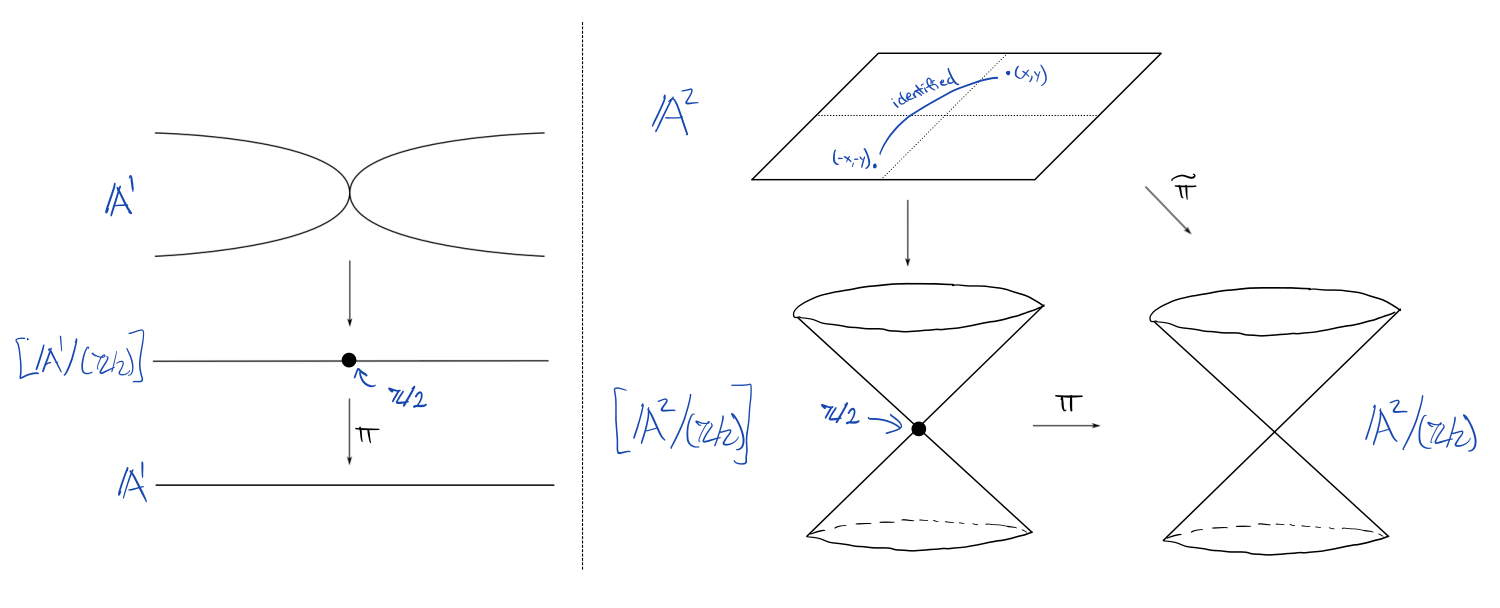
\includegraphics[width=0.95\textwidth]{figures/finite-quotients-source.png}};
\begin{scope}[x={(art.south east)},y={(art.north west)}]
\node[rotate=27,fill=white,inner sep=0.4pt,minimum width=2.7em,font=\scriptsize,text=blue!65!black]
 at (0.618,0.858) {等同};
\end{scope}
\end{tikzpicture}

\end{figure}
\end{example}

\subsection{不变量环的性质}\label{src:5.2.2-subsection}
\begin{lemma}\label{src:5.2.6}
若有限抽象群 $G$ 通过 $R$-代数自同构作用于 $R$-代数 $A$, 则 $A^G\to A$ 整. 若 $R$ 是 Noether 环且 $A$ 在 $R$ 上有限生成, 则 $A^G\to A$ 有限, 且 $A^G$ 在 $R$ 上有限生成.
\end{lemma}
\begin{proof}
为说明 $A^G\to A$ 整, 注意对每个元素 $a\in A$, 乘积 $\prod_{g\in G}(x-ga)\in A^G[x]$ 是具有不变系数且以 $a$ 为根的多项式. 若 $R$ 是 Noether 环, $R\to A$ 有限型, 则 $A^G\to A$ 也有限型. 由于 $A^G\to A$ 整且有限型, 它有限 (参见~\cite[推论 $5.2$]{AM69}). 由于 $R$ 是 Noether 环, 由 Artin--Tate 引理 (参见~\cite[命题 $7.8$]{AM69}) 可得 $R\to A^G$ 有限型.
\end{proof}
不变量环与平坦基变换相容.
\begin{lemma}\label{src:5.2.7}
设 $G$ 是作用于仿射概形 $\Spec A$ 的有限抽象群. 若 $A^G\to B$ 是平坦环同态, 则 $G$ 作用于仿射概形 $\Spec(B\otimes_{A^G}A)$, 且 $B=(B\otimes_{A^G}A)^G$.
\end{lemma}
\begin{proof}
按定义, 不变量环是等化子
\[
\begin{tikzcd}[column sep=large]
0\arrow[r]&A^G\arrow[r]&A\arrow[r,shift left,"p_1"]\arrow[r,shift right,"p_2"']&\displaystyle\prod_{g\in G}A,
\end{tikzcd}
\]
其中 $p_1(f)=(f)_{g\in G}$, $p_2(f)=(gf)_{g\in G}$. 由于 $A^G\to B$ 平坦,
\[
\begin{tikzcd}[column sep=large]
0\arrow[r]&B\arrow[r]&A\otimes_{A^G}B\arrow[r,shift left,"p_1"]\arrow[r,shift right,"p_2"']&\displaystyle\prod_{g\in G}A\otimes_{A^G}B
\end{tikzcd}
\]
也正合, 因而 $B=(B\otimes_{A^G}A)^G$.
\end{proof}
\newpage
\begin{exercise}\label{src:5.2.8}
设 $A^G\to B$ 是环同态, 考虑交换图
\[
\begin{tikzcd}[column sep=1.7em]
&\Spec B\otimes_{A^G}A\arrow[r]\arrow[d]\arrow[dl]&\Spec A\arrow[d]\\
\Spec(B\otimes_{A^G}A)^G\arrow[r]&\Spec B\arrow[r]\arrow[ur,phantom,"\square" description]&\Spec A^G.
\end{tikzcd}
\]
\begin{enumerate}[(a)]
\item 证明 $\Spec(B\otimes_{A^G}A)^G\to\Spec B$ 是整同胚.
\item 若 $|G|$ 在 $A$ 中可逆, 证明 $B\to(B\otimes_{A^G}A)^G$ 是同构.
\item 给出 $B\to(B\otimes_{A^G}A)^G$ 不是同构的例子.

\textit{提示:} 在特征 $p$ 时, 考虑 $\mathbb Z/p$ 在 $A=k[x,y]$ 上的作用, 其中生成元作用为 $(x,y)\mapsto(x+y,y)$, 并取 $B=A^G/(y)$.
\end{enumerate}
\end{exercise}

\subsection{粗模空间的性质}\label{src:5.2.3-subsection}
\begin{lemma}\label{src:5.2.9}
设 $\pi:\mathcal X\to X$ 是粗模空间, 满足对来自仿射概形的每个平展态射 $X'\to X$, 基变换 $\mathcal X\times_X X'\to X'$ 都是粗模空间. 则自然映射 $\mathcal O_X\to\pi_*\mathcal O_{\mathcal X}$ 是同构.
\end{lemma}
\begin{proof}
由于 $\pi$ 对到代数空间的映射具有泛性质, $\operatorname{Map}(X,\mathbb A^1)\to\operatorname{Map}(\mathcal X,\mathbb A^1)$ 是双射, 换言之, $\Gamma(X,\mathcal O_X)\cong\Gamma(\mathcal X,\mathcal O_{\mathcal X})$. 对每个平展映射 $X'\to X$, 基变换 $\mathcal X'=\mathcal X\times_X X'\to X'$ 也是粗模空间, 故 $\Gamma(X',\mathcal O_{X'})\cong\Gamma(\mathcal X',\mathcal O_{\mathcal X'})$. 这说明 $\mathcal O_X\to\pi_*\mathcal O_{\mathcal X}$ 是同构.
\end{proof}
为粗模空间的性质是平展局部的.
\begin{lemma}\label{src:5.2.10}
设 $\pi:\mathcal X\to X$ 是到代数空间的态射. 假设存在平展覆盖 $\{X_i\to X\}$, 使得对每个 $i$, $\mathcal X\times_X X_i\to X_i$ 是粗模空间. 则 $\pi:\mathcal X\to X$ 是粗模空间.
\end{lemma}
\begin{proof}
粗模空间的公理 (1) 是关于几何纤维的条件, 因而可在平展局部检验, 而公理 (2) 由代数空间是平展拓扑中的层这一事实推出.
\end{proof}

\subsection{\texorpdfstring{$\Spec A\to\Spec A^G$}{Spec A → Spec AG} 是几何商}\label{src:5.2.4-subsection}
\begin{proposition}\label{src:5.2.11}
若 $G$ 是作用于仿射概形 $\Spec A$ 的有限抽象群, 则 $\Spec A\to\Spec A^G$ 是几何商.
\end{proposition}
\begin{proof}
考虑交换图
\[
\begin{tikzcd}
U=\Spec A\arrow[d]\arrow[dr,"\widetilde\pi"]&\\
\mathcal X={[U/G]}\arrow[r,"\pi"']&X=\Spec A^G.
\end{tikzcd}
\]
由于 $\widetilde\pi$ 整且支配, 它满射. 为说明 $\widetilde\pi$ 在几何点的 $G$-轨道上单射, 设 $k$ 是代数闭域, 假设 $x,x'\in U(k)$ 在 $U\times_X k$ 上诱导的 $G$-作用下具有不同的 $G$-轨道. 由于这些轨道不交, 存在函数 $f\in A\otimes_{A^G}k$, 满足 $f|_{Gx}=0$, $f|_{Gx'}=1$. 则 $\widetilde f=\prod_{g\in G}gf\in(A\otimes_{A^G}k)^G$ 是 $G$-不变函数, 满足 $\widetilde f(x)=0$, $\widetilde f(x')=1$, 这蕴含 $\widetilde\pi(x)\neq\widetilde\pi(x')\in X(k)$.

还需说明自然映射
\begin{equation}\label{src:5.2.12}
\operatorname{Map}(X,Y)\longrightarrow\operatorname{Map}(\mathcal X,Y)
\end{equation}
对每个代数空间 $Y$ 都是双射. 注意当 $Y$ 仿射时这显然成立, 因为 $\Gamma(\mathcal X,\mathcal O_{\mathcal X})=\Gamma(X,\mathcal O_X)$. (当 $Y$ 是概形时, 不难归结到此情形: 若 $g:\mathcal X\to Y$ 是映射, 则 $Y$ 的仿射覆盖 $Y_i$ 诱导 $X$ 的开覆盖 $X_i=X\setminus\pi(\mathcal X\setminus g^{-1}(Y_i))$, $g$ 限制为映射 $\pi^{-1}(X_i)\to Y_i$, 由于 $\pi_*\mathcal O_{\mathcal X}=\mathcal O_X$, 它唯一经过 $X_i$ 分解; 另见~\cite[\S$0.6$]{GIT}.)

对于~\bookeqref{5.2.12} 的单射性, 设 $h_1,h_2:X\to Y$ 是满足 $h_1\circ\pi=h_2\circ\pi$ 的两个映射. 设 $E\to X$ 是 $h_1,h_2$ 的等化子, 即沿 $(h_1,h_2):X\to Y\times Y$ 拉回对角线 $Y\to Y\times Y$ 所得. 等化子 $E\to X$ 是单态射且局部有限型. 按构造 $\pi:\mathcal X\to X$ 经过 $E\to X$ 分解, 且由于 $\pi$ 普遍闭且\newterm{概形性支配}{schematically dominant} (即 $\mathcal O_X\to\pi_*\mathcal O_{\mathcal X}$ 单射), $E\to X$ 也如此. 每个普遍闭且局部有限型的单态射都是闭浸入 (见注记~\bookref{A.7.6}), 故 $E\to X$ 是同构.

对于~\bookeqref{5.2.12} 的满射性, 设 $g:\mathcal X\to Y$ 是态射. 先作一些容易的归约. 由引理~\bookref{5.2.7} 和~\bookref{5.2.10}, 问题在 $X$ 上是平展局部的; 特别地, 可假设 $X$ 仿射. 此外, 由于 $\mathcal X$ 拟紧, 映射 $g:\mathcal X\to Y$ 经过 $Y$ 的一个拟紧开代数子空间分解, 故可假设 $Y$ 拟紧. 设 $Y'\to Y$ 是来自仿射概形的平展呈示, 置 $\mathcal X':=\mathcal X\times_Y Y'$.

我们断言, 将 $X$ 换成平展覆盖 $V\to X$, 并将 $\mathcal X$ 换成基变换 $\mathcal X\times_X V$ 后, 在交换图
\[
\begin{tikzcd}
\mathcal X'\arrow[r]\arrow[d,"{g'}"']&\mathcal X\arrow[l,bend right=35,"s"']\arrow[r,"\pi"]\arrow[d,"g"]&X\arrow[dl,dashed]\\
Y'\arrow[r]\arrow[ur,phantom,"\square" description]&Y&
\end{tikzcd}
\]
中存在 $\mathcal X'\to\mathcal X$ 的截面 $s:\mathcal X\to\mathcal X'$.

\bookeqref{5.2.12} 的满射性由此断言推出: 由于 $X$ 与 $Y'$ 仿射, 等式 $\Gamma(X,\mathcal O_X)=\Gamma(\mathcal X,\mathcal O_{\mathcal X})$ 蕴含 $\mathcal X\xrightarrow{s}\mathcal X'\xrightarrow{g'}Y'$ 经由一个态射 $X\to Y'$ 通过 $\pi:\mathcal X\to X$ 分解. 复合 $X\to Y'\to Y$ 给出上图所需的虚线箭头.

为证明此断言, 使用极限方法进一步归结到 $X=\Spec A^G$ 为严格 Hensel 局部环的谱的情形. 对 $U:=\Spec A$ 中位于 $x\in|\mathcal X|$ 上方的闭点 $u$, 严格 Hensel 化 $X^{\mathrm{sh}}:=\mathcal O^{\mathrm{sh}}_{X,\pi(x)}$ 是所有 $\pi(x)$ 的仿射平展邻域 $X_\lambda\to X$ 的极限 $\lim_\lambda X_\lambda$. 基变换 $U^{\mathrm{sh}}:=U\times_X X^{\mathrm{sh}}$ 是仿射概形 $U_\lambda:=U\times_X X_\lambda$ 的极限. 再置 $\mathcal X^{\mathrm{sh}}:=\mathcal X\times_X X^{\mathrm{sh}}=[U^{\mathrm{sh}}/G]$, $\mathcal X_\lambda:=\mathcal X\times_X X_\lambda=[U_\lambda/G]$. 由于 $\mathcal X'\to\mathcal X$ 局部有限表现, 自然映射
\[
\mathrm{colim}_\lambda\operatorname{Mor}_{\mathcal X}(\mathcal X_\lambda,\mathcal X')\longrightarrow\operatorname{Mor}_{\mathcal X}(\mathcal X^{\mathrm{sh}},\mathcal X')
\]
是等价; 这由习题~\bookref{4.3.33} 推出 (该习题断言当第一项 $\mathcal X_\lambda$ 与 $\mathcal X^{\mathrm{sh}}$ 仿射时有此等式), 只需将 $\operatorname{Mor}_{\mathcal X}(\mathcal X^{\mathrm{sh}},\mathcal X')$ 表为 $\operatorname{Mor}_{\mathcal X}(U^{\mathrm{sh}},\mathcal X')\rightrightarrows\operatorname{Mor}_{\mathcal X}(G\times U^{\mathrm{sh}},\mathcal X')$ 的等化子, 左侧也同样处理. $\mathcal X'\times_{\mathcal X}\mathcal X^{\mathrm{sh}}\to\mathcal X^{\mathrm{sh}}$ 的截面由 $\mathcal X$ 上的映射 $\mathcal X^{\mathrm{sh}}\to\mathcal X'$ 确定. 该映射对某个 $\lambda$ 延伸为态射 $\mathcal X_\lambda\to\mathcal X'$, 给出所需截面.

设 $\kappa$ 是 $A^G$ 的剩余域. 由于 $A^G\to A$ 有限, $A=A_1\times\cdots\times A_r$ 是严格 Hensel 局部环的乘积, 每个因子都在 $A^G$ 上有限 (命题~\bookref{B.5.10}). 若 $u\in\Spec A_1\subseteq\Spec A$ 是闭点, 则 $\Spec A_1$ 是 $G_u$-不变的, 轨道 $Gu$ 与 $\Spec A$ 的 $r$ 个连通分支一一对应. 有同构 $\mathcal X\cong[\Spec A_1/G_u]$; 这可直接验证, 例如用 $\Spec A_1\hookrightarrow\Spec A$ 对群胚 $G\times\Spec A\rightrightarrows\Spec A$ 作切片 (如习题~\bookref{4.4.20}). 因此可将 $\mathcal X=[\Spec A/G]$ 换成 $[\Spec A_1/G_u]$, 并假设存在唯一闭点 $u\in\Spec A$, 且 $G$ 在集合意义下固定它. 由于 $Y'\to Y$ 可由概形表出, 可对某个概形 $U'$ 写成 $\mathcal X'=[U'/G]$. 设 $u'\in U'$ 是 $u\in\Spec A$ 的一个原像. 由于 $A$ 严格 Hensel, 且 $G$-等变态射 $U'\to U$ 是平展态射 $Y'\to Y$ 的基变换, 有 $\kappa(u')=\kappa(u)$, $G_{u'}=G_u=G$, 此外稳定子在剩余域上的作用平凡. 再次利用 $A$ 严格 Hensel, 存在唯一截面 $s:\Spec A\to U'$, 满足 $s(u)=u'$ (命题~\bookref{B.5.9}). 此截面 $G$-不变, 因为对每个 $g\in G$, $s\circ g$ 与 $g\circ s$ 都是 $U'\to\Spec A\xrightarrow{g^{-1}}\Spec A$ 的截面, 满足 $u'\mapsto u$, 故由截面的唯一性有 $s\circ g=g\circ s$. 于是 $s:\Spec AS\to U$ 下降为 $\mathcal X'\to\mathcal X$ 的截面 $\mathcal X=[\Spec A/G]\to[U'/G]=\mathcal X'$. 至此证明了 $\Spec A\to\Spec A^G$ 是几何商.
\end{proof}
现在不仅可得 $[\Spec A/G]\to\Spec A^G$ 是粗模空间, 还可得它具有定理~\bookref{5.2.3} 的性质 (1)--(4).
\begin{proof}[定理~\bookref{5.2.3} 的证明]
命题~\bookref{5.2.11} 蕴含 $\pi:[\Spec A/G]\to\Spec A^G$ 是粗模空间. 为说明性质 (1), 即 $\pi$ 是万有同胚, 注意由于 $\pi$ 双射且闭, 其集合意义下的逆映射连续, 故 $\pi$ 是同胚. 沿态射 $\Spec B\to\Spec A^G$ 对 $\pi$ 作基变换, 分解为
\[
{[\Spec(B\otimes_{A^G}A)/G]}\longrightarrow\Spec(B\otimes_{A^G}A)^G\longrightarrow\Spec B,
\]
其中第一映射由上述论证为同胚, 第二映射由习题~\bookref{5.2.8} 为同胚. 性质 (2), 即沿平坦态射 $X'\to\Spec A^G$ 对 $\pi$ 作基变换仍是粗模空间, 可先用引理~\bookref{5.2.10} 归结到 $X'$ 仿射的情形, 再由引理~\bookref{5.2.7} 推出. 性质 (3), 即 $\mathcal O_X\to\pi_*\mathcal O_{\mathcal X}$ 为同构, 由 (2) 及引理~\bookref{5.2.9} 直接推出. 最后, 引理~\bookref{5.2.6} 蕴含 (4): 若 $R$ 是 Noether 环, $R\to A$ 有限型, 则 $R\to A^G$ 有限型. 特别地, $A^G\to A$ 有限型, 而 $\pi:[\Spec A/G]\to\Spec A^G$ 分离, 普遍闭且有限型, 即固有.
\end{proof}
\begin{corollary}\label{src:5.2.13}
设 $G$ 是在仿射概形 $U=\Spec A$ 上自由作用的有限抽象群, 则代数空间商 $U/G$ 同构于 $\Spec A^G$.
\end{corollary}
\begin{proof}
代数空间商与几何商都对到代数空间的映射具有泛性质.
\end{proof}
\begin{exercise}\label{src:5.2.14}
设 $G$ 是作用于概形 $U$ 的有限抽象群.
\begin{enumerate}[(a)]
\item 证明几何商 $U/G$ 是概形, 当且仅当每个 $G$-轨道都包含在一个仿射开子概形中.
\item 若 $U$ 是 Noether 环 $R$ 上的仿射 (分别为拟仿射, 拟射影, 射影) 概形, 证明 $U/G$ 是 $R$ 上的仿射 (分别为拟仿射, 拟射影, 射影) 概形.
\end{enumerate}
\end{exercise}
\begin{exercise}\label{src:5.2.15}
假设有限抽象群 $G$ 作用于 Noether 环 $R$ 上的有限型仿射概形 $\Spec A$. 若 $x\in\Spec A$ 是闭点, 证明 $\Spec A$ 在 $x$ 处的完备化的 $G_x$-不变量与 $\Spec A^G$ 在 $x$ 的像处的完备化之间有同构
\[
\widehat A^{G_x}\cong\widehat{A^G}.
\]
\end{exercise}
以下习题将定理~\bookref{5.2.3} 从有限群的商推广到有限平坦群胚的商.
\begin{exercise}[困难]\label{src:5.2.16}
设 $s,t:R\rightrightarrows U$ 是仿射概形的有限平坦群胚, 定义 $A^R\subseteq A$ 为 $R$-不变量子环, 即由满足 $s^*a=t^*a\in\Gamma(R,\mathcal O_R)$ 的元素 $a\in A$ 组成的子环. 证明 $[U/R]\to X:=\Spec A^R$ 是具有定理~\bookref{4.4.13} 中性质 (1)--(4) 的粗模空间.

\textit{提示:} 为说明 $A^R\to A$ 整, 对元素 $a\in A$, 不使用引理~\bookref{5.2.6} 证明中的乘积 $\prod_{g\in G}(x-ga)\in A^G[x]$, 而使用 $\delta_0(a)\in B$ 的特征多项式, 其中将 $B$ 经由 $\delta_1$ 视作 $A$ 上的局部自由模, $\delta_0,\delta_1:A\rightrightarrows B=\Gamma(U,\mathcal O_U)$ 是两个有限平坦环映射. 另见~\cite[定理 V.4.1]{SGA3I}, \cite[命题 $5.1$]{KM97}, \cite[定理 $3.1$]{Con05b}, \cite[定理 $6.2.2$]{Ols16} 和~\cite[Tag 0DUR]{SP}.
\end{exercise}

% Source printed pp. 181-185 / PDF pp. 189-193.
\section{Deligne--Mumford 叠的局部结构}\label{src:5.3}
\begin{epigraph}
要是我有了那些定理就好了! 那么我就能轻易找出证明.
\epigraphauthor{相传出自 Bernhard Riemann}
\end{epigraph}
{\emergencystretch=3em
我们将说明, Deligne--Mumford 叠 $\mathcal X$ 在点 $x$ 附近, 在平展局部是仿射概形对稳定子群概形的商叠 $[\Spec A/G_x]$. 从概念上说, 这表明, 正如概形 (分别为代数空间) 由仿射概形在 Zariski 拓扑 (分别为平展拓扑) 中粘合而成, Deligne--Mumford 叠由商叠 $[\Spec A/G]$ 在平展拓扑中粘合而成.\footnote{当然, Deligne--Mumford 叠在平展局部也是概形, 但定理~\bookref{5.3.1} 所构造的平展邻域 $([\Spec A/G_x],w)\to(\mathcal X,x)$ 保持 $w$ 处的稳定子群.} 这一点的实际用途是, 它使我们能够将 Deligne--Mumford 叠的许多性质归结到商叠 $[\Spec A/G]$. 我们将利用局部结构定理构造粗模空间 (定理~\bookref{5.4.6}).\par}


\subsection{局部结构定理}\label{src:5.3.1-subsection}
Deligne--Mumford 叠 $\mathcal X$ 的点 $x\in|\mathcal X|$ 的\newterm{几何稳定子}{geometric stabilizer} 是如下定义的抽象群: 取任意像为 $x$ 的几何点 $\Spec k\to\mathcal X$, 并取其稳定子.
\begin{theorem}[Deligne--Mumford 叠的局部结构定理]\label{src:5.3.1}
设 $\mathcal X$ 是拟分离的 Deligne--Mumford 叠, $x\in|\mathcal X|$ 是有限型点, 几何稳定子为 $G_x$. 存在平展态射
\[
f:([\Spec A/G_x],w)\longrightarrow(\mathcal X,x),
\]
其中 $w\in[\Spec A/G_x]$, 使得 $f$ 在 $w$ 处诱导几何稳定子群的同构. 此外, 若 $\mathcal X$ 的对角线分离 (分别为仿射), 则可使 $f$ 可表出且分离 (分别为仿射).
\end{theorem}
\begin{proof}
先处理 $\mathcal X$ 的对角线仿射的情形. 选取代表 $x$ 的几何点 $\Spec k\to\mathcal X$, 设 $d$ 为 $G_x$ 的基数. 将 $G_x$ 看作 $\Spec k$ 上的群概形, 设 $BG_x\to\mathcal X$ 为所诱导的映射. 设 $(U,u)\to(\mathcal X,x)$ 是来自仿射概形的平展可表出态射. 由于 $\mathcal X$ 的对角线仿射, $U\to\mathcal X$ 仿射. 定义拟仿射概形
\[
\mathrm{SEC}_d:=\underbrace{U\times_{\mathcal X}\cdots\times_{\mathcal X}U}_{d\text{ 次}}\setminus\Delta,
\]
其中 $\Delta$ 是所有两两对角线的并. 来自概形的映射 $S\to\mathrm{SEC}_d$ 由一个态射 $S\to\mathcal X$ 以及 $U_S:=U\times_{\mathcal X}S\to S$ 的 $d$ 个不交截面 $s_1,\ldots,s_d$ (即当 $i\neq j$ 时, $s_i$ 与 $s_j$ 的交为空) 分类. 置换截面给出 $S_d$ 在 $\mathrm{SEC}_d$ 上的作用, 定义商叠
\[
\mathrm{ET}_d:=[\mathrm{SEC}_d/S_d].
\]
由主 $S_d$-丛与次数为 $d$ 的有限平展覆盖之间的对应 (习题~\bookref{B.1.55}), $\mathrm{ET}_d$ 在概形 $S$ 上的对象对应于图
\[
\begin{tikzcd}
Z\arrow[r,hook]\arrow[dr]&U_S\arrow[r]\arrow[d]&U\arrow[d]\\
&S\arrow[r]\arrow[ur,phantom,"\square" description]&\mathcal X,
\end{tikzcd}
\]
其中 $Z\hookrightarrow U_S$ 是闭子概形, $Z\to S$ 是次数为 $d$ 的有限平展态射. 有所诱导的平展态射 $\mathrm{ET}_d\to\mathcal X$ 以及交换图
\[
\begin{tikzcd}[column sep=large]
\mathrm{SEC}_d\arrow[r]\arrow[d,hook]&\mathrm{ET}_d\arrow[dr]&\\
U\times_{\mathcal X}\cdots\times_{\mathcal X}U\arrow[r]&U\arrow[r]&\mathcal X.
\end{tikzcd}
\]
为构造 $x$ 的一个原像 $w\in\mathrm{ET}_d(k)$, 注意纤维积 $BG_x\times_{\mathcal X}U$ 是有限个 $\Spec k$ 的不交并, 可以选取其中一个. 这给出交换图
\[
\begin{tikzcd}
\Spec k\arrow[r,hook]\arrow[dr]&\coprod\Spec k\arrow[r]\arrow[d]&U\arrow[d]\\
&BG_x\arrow[r]\arrow[ur,phantom,"\square" description]&\mathcal X,
\end{tikzcd}
\]
其中 $\Spec k\to BG_x$ 是次数为 $d$ 的有限平展态射, 这定义了 $BG_x\to\mathcal X$ 的提升 $BG_x\to\mathrm{ET}_d$. 复合 $w:\Spec k\to BG_x\to\mathrm{ET}_d$ 是 $x$ 的原像. 我们断言映射 $\mathrm{ET}_d\to\mathcal X$ 在 $w$ 处诱导几何稳定子的同构. 为说明这一点, 只需假设 $\mathcal X=BG_x$, $U=\Spec k$. 此时有同构 $U\times_{\mathcal X}\cdots\times_{\mathcal X}U\cong G_x^{d-1}$, 还可将其与对角作用的商 $G_x^d/G_x$ 等同. 于是 $\mathrm{SEC}_d\subseteq U\times_{\mathcal X}\cdots\times_{\mathcal X}U$ 与商 $(G_x^d\setminus\Delta)/G_x$ 等同. 置换作用 $S_d$ 是传递的, 其稳定子同构于 $G_x$. 事实上, $\mathrm{SEC}_d$ 与正则表示 $G\subseteq S_d$ 的商 $S_d/G$ 是 $S_d$-等变同构的, 因而 $\mathrm{ET}_d\cong BG_x$.

由于 $\mathrm{ET}_d$ 分离且 $\mathcal X$ 的对角线分离, 相对惯性叠 $I_{\mathrm{ET}_d/\mathcal X}\to\mathrm{ET}_d$ 有限. 由于 $\mathrm{ET}_d\to\mathcal X$ 在 $w$ 处诱导稳定子的同构, $I_{\mathrm{ET}_d/\mathcal X}\to\mathrm{ET}_d$ 在 $w$ 附近的某个开子叠 $[W/S_d]\subseteq\mathrm{ET}_d$ 上是同构, 其中 $W\subseteq\mathrm{SEC}_d$ 是拟仿射概形. 因此 $[W/S_d]\to\mathcal X$ 是分离, 平展且可表出的态射, 在 $w$ 处诱导稳定子群的同构. 改为对 $G_x\subseteq S_d$ 取商后, $[W/G_x]\to\mathcal X$ 同样是分离, 平展且可表出的态射, 在 $w$ 处诱导稳定子群的同构. 设 $W'\subseteq W$ 是包含 $w$ 的仿射开子概形, 可将 $W$ 换成 $G_x$-不变的仿射开子概形 $\bigcap_{g\in G_x}g\cdot W'$. 还需说明 $[W/G_x]\to\mathcal X$ 仿射. 由于 $\mathcal X$ 的对角线仿射, 来自仿射概形 $W$ 的态射 $W\to\mathcal X$ 仿射. 纤维积
\[
\begin{tikzcd}
{[W/G_x]}\times_{\mathcal X}W\arrow[r]\arrow[d]&W\arrow[d]\\
{[W/G_x]}\arrow[r]\arrow[ur,phantom,"\square" description]&\mathcal X
\end{tikzcd}
\]
在 $[W/G_x]$ 上仿射, 因而同构于商叠 $[\Spec B/G_x]$. 另一方面, 由于 $[W/G_x]\to\mathcal X$ 可表出, 商叠 $[\Spec B/G_x]$ 是代数空间, 且 $G_x$ 在 $\Spec B$ 上的作用自由. 由推论~\bookref{5.2.13}, $[\Spec B/G_x]$ 同构于仿射概形 $\Spec B^{G_x}$. 由平展下降, $[W/G_x]\to\mathcal X$ 仿射.

若 $\mathcal X$ 的对角线分离, 则上述论证给出具有 $G_x$ 作用的分离概形 $\mathrm{SEC}_d$, 以及分离, 平展且可表出的态射 $([\mathrm{SEC}_d/G_x],w)\to(\mathcal X,x)$, 在 $w$ 处诱导同构. 将论证再次用于分离的 Deligne--Mumford 叠 $[\mathrm{SEC}_d/G_x]$, 即得所需的局部商呈示. 若 $\mathcal X$ 仅拟分离, 则论证给出态射 $([\mathrm{SEC}_d/G_x],w)\to(\mathcal X,x)$ (不一定可表出), 在 $w$ 处诱导同构, 其中 $\mathrm{SEC}_d$ 是拟分离代数空间. 由于 $\mathrm{SEC}_d$ 的对角线分离 (因对角线是单态射), $[\mathrm{SEC}_d/S_d]$ 是具有分离对角线的 Deligne--Mumford 叠, 可以应用对角线分离情形的结论, 得到由仿射概形的商给出的局部商呈示. 另见~\cite[定理 $6.2$]{LMB00}.
\end{proof}
\begin{exercise}\label{src:5.3.2}
设 $\mathcal X$ 是 Deligne--Mumford 叠. 证明 $\mathcal X$ 同构于商叠 $[U/G]$, 其中 $U$ 是仿射概形 (分别为概形, 代数空间), $G$ 是有限抽象群, 当且仅当存在来自仿射概形 (分别为概形, 代数空间) 的有限平展态射 $V\to\mathcal X$.

\textit{提示:} 若 $V\to\mathcal X$ 是次数为 $d$ 的有限平展覆盖, 考虑如习题~\bookref{B.1.55} 中所述的相应主 $S_d$-torsor
\[
\underbrace{V\times_{\mathcal X}\cdots\times_{\mathcal X}V}_{d\text{ 次}}\setminus\Delta\longrightarrow\mathcal X.
\]
\end{exercise}
\begin{proposition}\label{src:5.3.3}
若 $R\rightrightarrows U$ 是仿射概形的有限平展等价关系, 则代数空间商 $U/R$ 是仿射概形.
\end{proposition}
\begin{proof}
由习题~\bookref{5.3.2}, 代数空间 $U/R$ 同构于 $V/G$, 其中有限群 $G$ 在仿射概形 $V=\Spec B$ 上自由作用. 定理~\bookref{5.2.3} 表明 $V/G\to\Spec B^G$ 对到代数空间的映射具有泛性质, 因而是同构. 也可由习题~\bookref{5.2.16} 推出: 若 $U=\Spec A$, 则 $U/R\to\Spec A^R$ 对到代数空间的映射具有泛性质, 因而是同构.
\end{proof}

\subsection{将有理点提升到呈示}\label{src:5.3.2-subsection}
使用与局部结构定理 (\bookref{5.3.1}) 的证明类似的技巧, 可证明存在能提升给定域值点的呈示.
\begin{proposition}\label{src:5.3.4}
若 $\mathcal X$ 是具有分离对角线的代数叠 (分别为具有分离且拟紧对角线的 Deligne--Mumford 叠), $x\in\mathcal X(k)$ 是域值点, 则存在来自仿射概形的光滑 (分别为平展) 态射 $U\to\mathcal X$, 以及位于 $x$ 上方的点 $u\in U(k)$.
\end{proposition}
\begin{proof}
设 $U\to\mathcal X$ 是来自仿射概形的光滑态射, 其像包含 $x$. 考虑纤维积
\[
\begin{tikzcd}
U_x\arrow[r]\arrow[d]&U\arrow[d]\\
\Spec k\arrow[r,"x"']\arrow[ur,phantom,"\square" description]&\mathcal X.
\end{tikzcd}
\]
由于 $\mathcal X$ 的对角线分离, 态射 $U\to\mathcal X$ 分离. 由于 $U_x$ 在 $\Spec k$ 上有限型且拟分离, 它是 Noether 代数空间. 选取闭点 $u\in U_x$, 由剩余 gerbe 的存在性 (\bookref{4.5.16}), 存在来自剩余域的闭浸入 $\Spec\kappa(u)\to U_x$. 域扩张 $k\to\kappa(u)$ 有限且可分, 设其次数为 $d$.

沿用定理~\bookref{5.3.1} 证明中的记号, 考虑参数化 $U\to\mathcal X$ 的 $d$ 个不交截面的开子空间 $\mathrm{SEC}_d\subseteq U\times_{\mathcal X}\cdots\times_{\mathcal X}U$, 它是分离代数空间. 定义分离的 Deligne--Mumford 叠 $\mathrm{ET}_d=[\mathrm{SEC}_d/S_d]$, 并考虑所诱导的态射 $\mathrm{ET}_d\to\mathcal X$. 由于 $\Spec\kappa(u)\to\Spec k$ 是次数为 $d$ 的有限平展态射, 闭浸入 $\Spec\kappa(u)\hookrightarrow U_x$ 定义 $\mathrm{ET}_d$ 的一个 $k$-点 $v$. 这给出交换图
\[
\begin{tikzcd}
&&\Spec k\arrow[dl,"v"']\arrow[d,"x"]\\
\mathrm{SEC}_d\arrow[r]&\mathrm{ET}_d\arrow[r]&\mathcal X.
\end{tikzcd}
\]
点 $v\in\mathrm{ET}_d(k)$ 不一定提升到 $\mathrm{SEC}_d$, 但可以用下面的技巧选取 $\mathrm{ET}_d$ 的另一种商呈示, 使 $v$ 可以提升.

具体而言, 选取忠实表示 $S_d\subseteq\GL_n$, 写成 $\mathrm{ET}_d\cong[V/\GL_n]$, 其中 $V=\mathrm{SEC}_d\times^{S_d}\GL_n$ 是分离代数空间. 于是 $v:\Spec k\to[V/\GL_n]$ 对应于主 $\GL_n$-丛 $P\to\Spec k$ 以及 $\GL_n$-等变映射 $P\to V$. 由于主 $\GL_n$-丛与向量丛一一对应 (习题~\bookref{B.1.58}), $P$ 是平凡主 $\GL_n$-丛, 存在截面 $\Spec k\to P$. 复合 $V\to[V/\GL_n]\to\mathcal X$ 光滑, 复合 $\Spec k\to P\to V$ 是 $x$ 的提升.

由于 $V$ 是分离代数空间, 问题归结为证明第二个陈述, 即具有分离且拟紧对角线的 Deligne--Mumford 叠 $\mathcal X$ 的 $k$-点可提升到来自概形的平展邻域. 将用到 $\mathcal X$ 的对角线拟仿射这一事实, 它将在后面的推论~\bookref{5.5.8} 中独立证明 (证明只用到上面的命题~\bookref{5.3.3} 以及~\S\bookref{5.1} 中的拟凝聚层理论). 重复上述论证, 选取来自仿射概形的平展映射 $U\to\mathcal X$, 其像包含 $x$. 则 $U\to\mathcal X$ 的 $d$ 个不交截面的空间 $\mathrm{SEC}_d$ 是拟仿射概形, 且带有 $S_d$ 的自由作用. 商 $\mathrm{ET}_d=\mathrm{SEC}_d/S_d$ 也是拟仿射的 (习题~\bookref{5.2.14}). 所诱导的映射 $\mathrm{ET}_d\to\mathcal X$ 平展, 且按构造 $k$-点 $x$ 提升为 $\mathrm{ET}_d$ 的 $k$-点. 另见~\cite[定理 $6.3$]{LMB00}.
\end{proof}
还有局部结构定理的另一个版本, 在粗模空间上以平展局部的方式表述 (见推论~\bookref{5.4.13}).

% Source printed pp. 185-195 / PDF pp. 193-203.
\section{粗模空间与 Keel--Mori 定理}\label{src:5.4}
\begin{epigraph}
至于 $M_g$, 几乎毫无疑问, 可以赋予它代数簇的结构.
\epigraphauthor{André Weil~\cite[第 $383$ 页]{Wei58}}
\end{epigraph}
我们将证明, Noether 概形上的每个分离有限型 Deligne--Mumford 叠 $\mathcal X$ 都有分离的粗模空间 $\pi:\mathcal X\to X$, 称为 Keel--Mori 定理 (\bookref{5.4.6}). 可将此定理视为消去 Deligne--Mumford 叠的叠性的一种方式: 以牺牲 $\mathcal X$ 的泛性质 (例如万有族的存在性) 为代价, 可以用代数空间替换 $\mathcal X$, 而不改变底层拓扑空间. 引入稳定曲线的 Deligne--Mumford 叠 $\overline{\mathcal M}_g$ (定理~\bookref{6.4.16}) 并证明它分离 (命题~\bookref{6.5.20}) 后, Keel--Mori 定理蕴含存在粗模空间 $\overline{\mathcal M}_g\to\overline M_g$, 其中 $\overline M_g$ 是分离代数空间. 此外, 半稳定约化 (\bookref{6.5.9}), 即 $\overline{\mathcal M}_g$ 的固有性, 进一步蕴含 $\overline M_g$ 固有. 在~\S\bookref{6.8} 和~\S\bookref{6.9} 中, 我们将给出 $\overline M_g$ 射影性的两个证明.

粗模空间已在定义~\bookref{5.2.1} 中引入. 若 $G$ 是作用于仿射概形 $\Spec A$ 的有限抽象群, 则 $[\Spec A/G]\to\Spec A^G$ 是粗模空间 (定理~\bookref{5.2.3}), 换言之 $\Spec A\to\Spec A^G$ 是几何商. 为证明 Keel--Mori 定理 (\bookref{5.4.6}), 将应用局部结构定理 (\bookref{5.3.1}) 构造平展邻域 $[\Spec A_i/G]\to\mathcal X$, 再在平展拓扑中粘合几何商 $\Spec A_i^G$, 从而构造 $\mathcal X$ 的粗模空间.

\subsection{将平展态射下降到几何商}\label{src:5.4.1-subsection}
为在平展拓扑中粘合几何商, 需要一个条件, 保证平展 $G$-等变态射 $\Spec A\to\Spec B$ 在几何商上诱导平展态射 $\Spec A^G\to\Spec B^G$. 以下命题可视为 Luna 基本引理 (\bookref{7.5.30}) 的初步版本.
\begin{proposition}\label{src:5.4.1}
设 $G$ 是有限抽象群, $f:\Spec A\to\Spec B$ 是 Noether 环 $R$ 上有限型仿射概形的 $G$-等变态射. 设 $x\in\Spec A$ 是闭点. 假设
\begin{enumerate}[(a)]
\item $f$ 在 $x$ 处平展, 且
\item 所诱导的稳定子群概形的映射 $G_x\to G_{f(x)}$ 是双射.
\end{enumerate}
则 $x$ 的像在 $\Spec A^G$ 中有仿射开邻域 $W$, 使得 $W\to\Spec A^G\to\Spec B^G$ 平展, 且 $\pi_A^{-1}(W)\cong W\times_{\Spec B^G}[\Spec B/G]$, 其中 $\pi_A:[\Spec A/G]\to\Spec A^G$.
\end{proposition}
\begin{remark}\label{src:5.4.2}
换言之, 将 $\Spec A^G$ 换成 $\pi_A(x)$ 的仿射邻域 $W$, 并将 $\Spec A$ 换成 $\pi_A^{-1}(W)$ 后, 可使图
\begin{equation}\label{src:5.4.3}
\begin{tikzcd}
{[\Spec A/G]}\arrow[r,"f"]\arrow[d,"\pi_A"']&{[\Spec B/G]}\arrow[d,"\pi_B"]\\
\Spec A^G\arrow[r]\arrow[ur,phantom,"\square" description]&\Spec B^G
\end{tikzcd}
\end{equation}
为 Cartesian 图, 其中两个水平映射均平展.
\end{remark}
\begin{proof}[命题~\bookref{5.4.1} 的证明]
置 $y=f(x)$. 首先断言, 问题在 $\pi_B(y)\in\Spec B^G$ 附近是平展局部的. 事实上, 若 $Y'\to Y:=\Spec B^G$ 是 $\pi_B(y)$ 的仿射平展邻域, 用 $X'$, $\mathcal X'$ 和 $\mathcal Y'$ 分别表示 $X:=\Spec A^G$, $\mathcal X:=[\Spec A/G]$ 和 $\mathcal Y:=[\Spec B/G]$ 的基变换. 由引理~\bookref{5.2.7}, 有 $\mathcal Y'\cong[\Spec B'/G]$, $Y'\cong\Spec B'{}^G$, 对 $\mathcal X'$ 与 $X'$ 也类似. 若结果在此基变换后成立, 则存在包含 $\pi_A(x)$ 的某个原像的开邻域 $W'\subseteq X'$, 使得 $W'\hookrightarrow X'\to Y'$ 平展, 且 $W'$ 在 $\mathcal X'$ 中的原像同构于 $W'\times_{Y'}\mathcal Y'$. 取 $W$ 为 $W'$ 在 $X'\to\Spec A^G$ 下的像, 再应用平展下降, 即得所需断言.

现在断言, 由此可假设 $B^G$ 是严格 Hensel 环. 为此, 定义 $Y^{\mathrm{sh}}=\Spec\mathcal O^{\mathrm{sh}}_{Y,\pi_B(y)}$, 用 $X^{\mathrm{sh}}$, $\mathcal X^{\mathrm{sh}}$ 和 $\mathcal Y^{\mathrm{sh}}$ 表示 $X$, $\mathcal X$ 和 $\mathcal Y$ 沿 $Y^{\mathrm{sh}}\to Y$ 的基变换. 可将 $Y^{\mathrm{sh}}=\lim_\lambda Y_\lambda$ 写成 $y$ 的仿射平展邻域 $Y_\lambda\to Y$ 的极限, 用 $X_\lambda$, $\mathcal X_\lambda$ 和 $\mathcal Y_\lambda$ 表示 $X$, $\mathcal X$ 和 $\mathcal Y$ 沿 $Y_\lambda\to Y$ 的基变换. 假设 $U^{\mathrm{sh}}\subseteq X^{\mathrm{sh}}$ 是包含位于 $x$ 及 $Y^{\mathrm{sh}}$ 的闭点上方的唯一点的仿射开子概形, 使得 $U^{\mathrm{sh}}\to Y^{\mathrm{sh}}$ 平展, 且
\[
\pi_{\mathcal X^{\mathrm{sh}}}^{-1}(U^{\mathrm{sh}})\cong U^{\mathrm{sh}}\times_{Y^{\mathrm{sh}}}\mathcal Y^{\mathrm{sh}}.
\]
由命题~\bookref{B.3.3}, 态射 $U^{\mathrm{sh}}\to X^{\mathrm{sh}}$ 对某个 $\eta$ 下降为 $U_\eta\to X_\eta$. 对 $\lambda>\eta$ 置 $U_\lambda=U_\eta\times_{X_\eta}X_\lambda$. 由命题~\bookref{B.3.7}, 对 $\lambda\gg0$ 有
\begin{enumerate}[(a)]
\item $U_\lambda\to X_\lambda$ 是开浸入;
\item 复合 $U_\lambda\to X_\lambda\to Y_\lambda$ 平展; 且
\item $\pi_{\mathcal X_\lambda}^{-1}(U_\lambda)\cong U_\lambda\times_{Y_\lambda}\mathcal Y_\lambda$ (在 $\mathcal X$ 与 $\mathcal Y$ 的平展呈示上论证).
\end{enumerate}
最后, 由于 $B^G\to B$ 有限 (引理~\bookref{5.2.6}), $B=B_1\times\cdots\times B_r$ 是严格 Hensel 局部环的乘积 (命题~\bookref{B.5.10}). 如定理~\bookref{5.2.3} 的证明, 可将 $[\Spec B/G]$ 换成 $[\Spec B_1/G_y]$, 将 $[\Spec A/G]$ 换成 $[f^{-1}(\Spec B_1)/G]$, 从而假设 $G$ 固定 $x$ 与 $y$, 且在剩余域 $\kappa(x)=\kappa(y)$ 上作用平凡. 因此 $\Spec A\to\Spec B$ 有将 $y$ 送到 $x$ 的唯一截面 $s:\Spec B\to\Spec A$. 截面 $s$ 必为 $G$-不变的 (如定理~\bookref{5.2.3} 的证明). 于是 $s$ 下降为 $\Spec A^G\to\Spec B^G$ 的截面, 给出所需的开闭子概形 $W\subseteq\Spec A^G$.
\end{proof}
\begin{remark}\label{src:5.4.4}
以下从概念上解释为何应当期待所诱导的商映射平展. 为简单起见, 假设 $R=k$ 是代数闭域. 设 $\widehat A$ 与 $\widehat B$ 是 $x$ 与 $f(x)$ 处局部环的完备化. 稳定子 $G_x$ 与 $G_{f(x)}$ 分别作用于 $\Spec\widehat A$ 与 $\Spec\widehat B$, 映射 $\Spec\widehat A\to\Spec\widehat B$ 关于映射 $G_x\to G_{f(x)}$ 等变. $A^G$ 在 $x$ 的像处的完备化 $\widehat{A^G}$ 同构于 $\widehat A^{G_x}$ (习题~\bookref{5.2.15}), 类似地 $\widehat{B^G}=\widehat B^{G_{f(x)}}$. 由于 $f$ 在 $x$ 处平展, $\widehat B\to\widehat A$ 是同构, 又因 $G_x\to G_{f(x)}$ 是双射, 所诱导的映射 $\widehat{B^G}\to\widehat{A^G}$ 是同构, 这说明 $\Spec A^G\to\Spec B^G$ 在 $x$ 的像处平展.
\end{remark}
上述命题将在 Keel--Mori 定理 (\bookref{5.4.6}) 的证明中以下列形式应用.
\begin{corollary}\label{src:5.4.5}
设 $G$ 是有限抽象群, $f:\Spec A\to\Spec B$ 是 Noether 环 $R$ 上有限型仿射概形的 $G$-等变态射. 假设对每个闭点 $x\in\Spec A$,
\begin{enumerate}[(a)]
\item $f$ 在 $x$ 处平展, 且
\item 所诱导的稳定子群概形的映射 $G_x\to G_{f(x)}$ 是双射.
\end{enumerate}
则 $\Spec A^G\to\Spec B^G$ 平展, 且~\bookeqref{5.4.3} 是 Cartesian 图.
\end{corollary}

\subsection{Keel--Mori 定理}\label{src:5.4.2-subsection}
现在陈述并证明 Keel--Mori 定理.
\begin{theorem}[Keel--Mori 定理]\label{src:5.4.6}
设 $\mathcal X$ 是 Noether 代数空间 $S$ 上的分离有限型 Deligne--Mumford 叠. 则存在粗模空间 $\pi:\mathcal X\to X$, 满足 $\mathcal O_X=\pi_*\mathcal O_{\mathcal X}$, 且
\begin{enumerate}[(1)]
\item $X$ 在 $S$ 上分离且有限型;
\item $\pi$ 是固有万有同胚; 且
\item 对代数空间的每个平坦态射 $X'\to X$, 基变换 $\mathcal X\times_X X'\to X'$ 是粗模空间.
\end{enumerate}
此外, $X$ 固有, 当且仅当 $\mathcal X$ 固有.
\end{theorem}
此定理可推广到满足 $I_{\mathcal X}\to\mathcal X$ 有限的 Deligne--Mumford 叠 $\mathcal X$ (可能不分离), 只是其粗模空间可能不分离 (习题~\bookref{5.4.10}). 更为有力的是, Keel--Mori 定理~\cite{KM97} 在将 $\mathcal X$ 是 Deligne--Mumford 叠的假设换成 $\mathcal X$ 是具有有限惯性 $I_{\mathcal X}\to\mathcal X$ 的代数叠这一假设后仍成立; 见注记~\bookref{5.4.11}. 这要求所有稳定子有限, 但不一定约化. 此定理在不加任何 Noether 性或有限性条件时也成立; 见~\cite{Con05b}, \cite{Ryd13} 和~\cite[Tag 0DUK]{SP}.
\begin{remark}[历史注记]\label{src:5.4.7}
大约与~\cite{KM97} 发表同时, Kollár 证明了一个重要特例, 已足以用于许多应用: 若 $G$ 是优良概形 $S$ 上的仿射群概形, 在 $S$ 上的分离代数空间 $U$ 上固有作用, 且 $G\to S$ 是约化群概形, 或者 $S=\Spec k$, $\operatorname{char}(k)>0$, 则存在分离几何商 $U/G$~\cite[定理 $1.5$]{Kol97}. 在这些文章之前, 粗模空间的存在性被视为熟知定理, 但分离 Deligne--Mumford 叠情形的陈述和证明无疑早已为专家所知. 例如, \cite[定理 I.4.10]{FC90} 和~\cite[定理 $2.2$]{Kol90} 中明确陈述了此定理, 但未给出证明. Popp 在~\cite[第 $55$ 页的定理]{Pop74} 中, 对 $\mathbb C$ 上群作用的情形勾勒了使用解析技巧的论证, 而~\cite[\S$5$.A]{MF82} 中勾勒了解析和代数两种论证.

由于 $\mathcal M_g$ 是 $\mathbb Z$ 上的分离有限型 Deligne--Mumford 叠 (推论~\bookref{4.6.10} 和习题~\bookref{4.8.12}), Keel--Mori 定理蕴含存在作为分离代数空间的粗模空间 $\mathcal M_g\to M_g$. 此结果最初归功于 Mumford, 他证明了更强的结果, 即 $M_g$ 作为概形存在. 在~\cite{Mum61} 中勾勒证明之后, Mumford 在~\cite[定理 $5.11$ 和 $7.13$]{GIT} 中给出 $\Spec\mathbb Z$ 上 $M_g$ 的两种构造. 此外, 他证明对每个素数 $p$, $M_g$ 在 $\Spec\mathbb Z[1/p]$ 上拟射影. 后来证明了 $\overline M_g$ 在 $\Spec\mathbb Z$ 上射影, 特别地 $M_g$ 在 $\Spec\mathbb Z$ 上拟射影; 见~\S\bookref{6.8}--\bookref{6.9}. 有趣的是, Mumford 的两种构造实际都没有使用 GIT, 或至少没有使用通常被视为``标准 GIT 工具''的部分, 我们将在~\S\bookref{8.4} 中发展这些工具. Mumford 的一种构造依赖主极化 Abel 簇的模空间 $A_g$ 的存在性, 另一种则依赖使用协变式的专门方法.
\end{remark}
\begin{remark}\label{src:5.4.8}
强调此定理不仅给出粗模空间, 而且给出的粗模空间满足性质 (1)--(3). 仅满足定义中性质 (定义~\bookref{5.2.1}) 的粗模空间可能难以使用. 例如, 一般情况下尚不清楚粗模空间是否在平展基变换 (甚至开浸入) 下稳定, 或是否满足 $\pi_*\mathcal O_{\mathcal X}=\mathcal O_X$.
\end{remark}
\begin{proof}
先处理 $S=\Spec R$ 仿射的情形. 问题在 $\mathcal X$ 上是 Zariski 局部的: 若 $\{\mathcal X_i\}$ 是 $\mathcal X$ 的 Zariski 开覆盖, 且各项有粗模空间 $\mathcal X_i\to X_i$, 则由于粗模空间唯一 (定义~\bookref{5.2.1}(2)), 每个交 $\mathcal X_i\cap\mathcal X_j$ 都有粗模空间 $U_{ij}$, 可与 $X_i$ 和 $X_j$ 的开子概形等同, 从而可粘合得到代数空间 $X$ 以及映射 $\mathcal X\to X$. 由引理~\bookref{5.2.10}, 它是粗模空间. 因此只需说明每个闭点 $x\in|\mathcal X|$ 都有一个存在粗模空间的开邻域.

由 Deligne--Mumford 叠的局部结构定理 (\bookref{5.3.1}), 存在仿射平展态射
\[
f:(\mathcal W=[\Spec A/G_x],w)\longrightarrow(\mathcal X,x),
\]
使得 $f$ 在 $w$ 处诱导几何稳定子群的同构. 断言由满足 $f$ 在 $z$ 处诱导几何稳定子群同构的点 $z\in|\mathcal W|$ 组成的轨迹 $\mathcal U$ 是开的. 为证明这一点, 利用相对惯性 $I_{\mathcal X}\to\mathcal X$ 有限这一事实, 它由 $\mathcal X$ 的分离性推出 (因为对角线固有且拟有限). $\mathcal W$ 上相对群概形的自然态射 $I_{\mathcal W}\to I_{\mathcal X}\times_{\mathcal X}\mathcal W$ 在 $z\in\mathcal W(k)$ 上方的纤维正是稳定子的态射 $G_z\to G_{f(z)}$. 将使用习题~\bookref{4.2.15} 中的 Cartesian 图
\[
\begin{tikzcd}
I_{\mathcal W}\arrow[r,"\Psi"]\arrow[d]&I_{\mathcal X}\times_{\mathcal X}\mathcal W\arrow[d]\\
\mathcal W\arrow[r]\arrow[ur,phantom,"\square" description]&\mathcal W\times_{\mathcal X}\mathcal W.
\end{tikzcd}
\]
由于 $\mathcal W\to\mathcal X$ 可表出, 平展且分离, 对角线 $\mathcal W\to\mathcal W\times_{\mathcal X}\mathcal W$ 是开闭浸入, 因而 $\Psi$ 也是如此. 由于 $I_{\mathcal X}\to\mathcal X$ 有限, $p_2:I_{\mathcal X}\times_{\mathcal X}\mathcal W\to\mathcal W$ 也有限. 因此
\[
p_2\bigl(|I_{\mathcal X}\times_{\mathcal X}\mathcal W|\setminus|I_{\mathcal W}|\bigr)\subseteq|\mathcal W|
\]
是闭的, 它的补集与轨迹 $\mathcal U$ 等同, 因而是开的. 设 $\pi_{\mathcal W}:\mathcal W\to W=\Spec A^{G_x}$ 是粗模空间 (定理~\bookref{5.2.3}). 选取包含 $\pi_{\mathcal W}(w)$ 的仿射开子概形 $X_1\subseteq\pi(\mathcal U)$. 则 $\mathcal X_1=\pi_{\mathcal W}^{-1}(X_1)$ 同构于商叠 $[\Spec A_1/G_x]$, 且 $X_1=\Spec A_1^{G_x}$. 这给出仿射平展态射
\[
g:(\mathcal X_1=[\Spec A_1/G_x],w)\longrightarrow(\mathcal X,x),
\]
在所有几何稳定子群上诱导双射.

现在说明开子叠 $\mathcal X_0:=\operatorname{im}(f)$ 有粗模空间. 由于 $g$ 仿射且 $\mathcal X_1=[\Spec A_1/G_x]$, 可将 $\mathcal X_2:=\mathcal X_1\times_{\mathcal X}\mathcal X_1$ 表为 $[\Spec A_2/G_x]$, 并有粗模空间 $\pi_2:\mathcal X_2\to X_2=\Spec A_2^{G_x}$. 由粗模空间的泛性质, 有图
\begin{equation}\label{src:5.4.9}
\begin{tikzcd}[column sep=large]
\mathcal X_2\arrow[r,shift left]\arrow[r,shift right]\arrow[d,"\pi_2"']&\mathcal X_1\arrow[r,"g"]\arrow[d,"\pi_1"]&\mathcal X_0=\operatorname{im}(g)\arrow[d,dashed,"\pi_0"]\\
X_2\arrow[r,shift left]\arrow[r,shift right]\arrow[ur,phantom,"\square" description]&X_1\arrow[r,dashed]&X_0,
\end{tikzcd}
\end{equation}
其中自然方块交换. 由于 $g$ 在所有点的几何稳定子群上诱导双射, 每个投影 $\mathcal X_2\to\mathcal X_1$ 也如此. 推论~\bookref{5.4.5} 蕴含每个映射 $X_2\to X_1$ 平展, 且~\bookeqref{5.4.9} 中实线箭头的自然方块是 Cartesian 的.

粗模空间的泛性质诱导平展群胚结构 $X_2\rightrightarrows X_1$. 为检验它是平展等价关系, 只需检验 $X_2\to X_1\times X_1$ 在几何点上单射, 这由 $|\mathcal X_2|\to|\mathcal X_1|\times|\mathcal X_1|$ 在闭点上单射这一观察推出. 因此存在代数空间商 $X_0:=X_1/X_2$ 以及映射 $X_1\to X_0$. 沿 $\mathcal X_1\to\mathcal X_0$ 作平展下降, 得到映射 $\pi_0:\mathcal X_0\to X_0$, 使~\bookeqref{5.4.9} 的右方块交换.

为说明 $\pi:\mathcal X_0\to X_0$ 是粗模空间, 将使用交换立方体
\[
\begin{tikzcd}[row sep=1.4em,column sep=1.6em]
&\mathcal X_2\arrow[rr]\arrow[dl]\arrow[dd]&&\mathcal X_1\arrow[dl]\arrow[dd]\\
\mathcal X_1\arrow[rr,crossing over]\arrow[dd]&&\mathcal X_0\arrow[dd]&\\
&X_2\arrow[rr]\arrow[dl]&&X_1\arrow[dl]\\
X_1\arrow[rr]&&X_0.&
\end{tikzcd}
\]
其中上面, 左面和下面是 Cartesian 的. 由于 $\mathcal X_1\to\mathcal X_0$ 平展且满射, 自然映射 $\mathcal X_1\to\mathcal X_0\times_{X_0}X_1$ 拉回后为同构, 故 $\mathcal X_1\cong\mathcal X_0\times_{X_0}X_1$, 右方块也为 Cartesian 的. 由于为粗模空间的性质在 $X_0$ 上是平展局部的 (引理~\bookref{5.2.10}), 得到 $\pi_0:\mathcal X_0\to X_0$ 是粗模空间. $\mathcal O_{X_0}\to\pi_{0,*}\mathcal O_{\mathcal X_0}$ 的条件及性质 (1)--(3) 也都是平展局部的, 且由定理~\bookref{5.2.3}, 它们对 $[\Spec A_1/G_x]\to\Spec A_1^{G_x}$ 成立, 故也对 $\mathcal X_0\to X_0$ 成立.

$S$ 为 Noether 代数空间的情形, 可仿照上述论证, 在平展局部构造 $\mathcal X$ 的粗模空间, 从而归结到仿射情形. 最后, 由于 $\mathcal X_0\to X_0$ 固有, $\mathcal X_0$ 的分离性等价于 $X_0$ 的分离性.
\end{proof}
\begin{exercise}\label{src:5.4.10}
若 $\mathcal X$ 是 Noether 代数空间 $S$ 上的有限型 Deligne--Mumford 叠, 且 $I_{\mathcal X}\to\mathcal X$ 有限, 则存在粗模空间 $\pi:\mathcal X\to X$, 满足 $\mathcal O_X=\pi_*\mathcal O_{\mathcal X}$, 并具有定理~\bookref{5.4.6} 的性质 (1)--(3).
\end{exercise}
\begin{remark}\label{src:5.4.11}
$\mathcal X$ 为具有有限惯性 $I_{\mathcal X}\to\mathcal X$ 的代数叠 (不一定为 Deligne--Mumford 叠) 的更一般情形, 可用类似但更为技术性的方式证明:
\begin{enumerate}[{步骤} 1:]
\item 构造来自概形的拟有限平坦满射 $U\to\mathcal X$. 证明与极小呈示的存在性 (\bookref{4.6.1}) 类似; 见注记~\bookref{4.6.2}, \cite[引理 V.7.2]{SGA3I}, \cite[引理 $3.3$]{KM97}, \cite[引理 $2.1$]{Con05b} 和~\cite[Tag 06MC]{SP}.
\item 说明每个点都有平展邻域 $\mathcal W\to\mathcal X$, 其中 $\mathcal W$ 有来自仿射概形的有限平坦呈示 $V\to\mathcal W$. 这应当视为 Deligne--Mumford 叠局部结构定理 (\bookref{5.3.1}) 的替代: $\mathcal W$ 不再是有限群的商 $[\Spec A/G]$, 而是仿射概形的有限平坦群胚 $R:=V\times_{\mathcal W}V\rightrightarrows V$ 的商 $[V/R]$. 证明也类似: 不使用 $\mathrm{ET}_d:=[(U\times_{\mathcal X}\cdots\times_{\mathcal X}U\setminus\Delta)/S_d]$ 参数化 $U\to\mathcal X$ 的纤维中的 $d$ 个无序点, 而使用 $\mathcal X$ 上的相对 Hilbert 叠 $\mathcal{H}ilb_d$, 其在 $S\to\mathcal X$ 上的对象由闭子概形 $Z\hookrightarrow U\times_{\mathcal X}S$ 组成, 在 $S$ 上有限平坦 (而非有限平展), 次数为 $d$. 见~\cite[\S$5$.A]{MF82}, \cite[命题 $4.2$]{KM97}, \cite[引理 $2.2$]{Con05b} 和~\cite[Tag 0DU4]{SP}.
\item 证明仿射概形的有限平坦群胚 $R\rightrightarrows V$ 的商 $[R/V]$ 的群胚存在性. 证明与定理~\bookref{5.2.3} 类似; 见习题~\bookref{5.2.16}, \cite[定理 V.4.1]{SGA3I}, \cite[命题 $5.1$]{KM97}, \cite[定理 $3.1$]{Con05b}, \cite[定理 $6.2.2$]{Ols16} 和~\cite[Tag 0DUR]{SP}.
\end{enumerate}
\end{remark}
\begin{corollary}\label{src:5.4.12}
若 $G$ 是 Noether 概形 $S$ 上的仿射 fppf 群概形, 在分离代数空间 $U$ 上固有作用, 即作用映射 $G\times U\to U\times U$ 固有, 且所有稳定子群均约化, 则存在到 $S$ 上分离有限型代数空间 $X$ 的几何商 $\pi:U\to X$, 满足 $\mathcal O_X=(\pi_*\mathcal O_U)^G$.
\end{corollary}
\begin{proof}
由于 $G$ 在 $S$ 上仿射, $\sigma:G\times U\to U\times U$ 仿射. 因此 $\sigma$ 的固有性等价于 $U$ 的有限性, 并蕴含 $[U/G]$ 的对角线有限. 由于稳定子群约化, $[U/G]$ 是分离的 Deligne--Mumford 叠, 从而可应用 Keel--Mori 定理 (\bookref{5.4.6}).
\end{proof}
证明中粗模空间的构造给出粗模空间的局部结构定理. (也可直接由局部结构定理 (\bookref{5.3.1}) 和习题~\bookref{5.4.14} 得到以下定理.)
\begin{corollary}[粗模空间的局部结构]\label{src:5.4.13}
设 $\mathcal X$ 是 Noether 代数空间 $S$ 上的有限型分离 Deligne--Mumford 叠, $\pi:\mathcal X\to X$ 是其粗模空间. 对每个闭点 $x\in|\mathcal X|$, 设其几何稳定子群为 $G_x$, 则存在 Cartesian 图
\[
\begin{tikzcd}
{[\Spec A/G_x]}\arrow[r]\arrow[d]&\mathcal X\arrow[d,"\pi"]\\
\Spec A^{G_x}\arrow[r]\arrow[ur,phantom,"\square" description]&X,
\end{tikzcd}
\]
使得 $\Spec A^{G_x}\to X$ 是 $\pi(x)\in|X|$ 的平展邻域.
\end{corollary}
\begin{exercise}\label{src:5.4.14}
建立命题~\bookref{5.4.1} 的以下推广: 若 $f:\mathcal X\to\mathcal Y$ 是 Noether 代数空间 $S$ 上分离有限型 Deligne--Mumford 叠的态射, 位于交换图
\[
\begin{tikzcd}
\mathcal X\arrow[r,"f"]\arrow[d,"\pi_{\mathcal X}"']&\mathcal Y\arrow[d,"\pi_{\mathcal Y}"]\\
X\arrow[r]&Y
\end{tikzcd}
\]
中, 其中 $\pi_{\mathcal X}:\mathcal X\to X$ 和 $\pi_{\mathcal Y}:\mathcal Y\to Y$ 是粗模空间, 且 $x\in|\mathcal X|$ 是满足以下条件的闭点:
\begin{enumerate}[(1)]
\item $f$ 在 $x$ 处平展; 且
\item 所诱导的几何稳定子群映射 $G_x\to G_{f(x)}$ 是双射,
\end{enumerate}
则 $\pi_{\mathcal X}(x)$ 有开邻域 $U\subseteq X$, 使得 $U\to X\to Y$ 平展, 且 $\pi_{\mathcal X}(U)\cong U\times_Y\mathcal Y$.
\end{exercise}

\subsection{例子}\label{src:5.4.3-subsection}
粗模空间的基本例子是有限群作用所诱导的映射 $[\Spec A/G]\to\Spec A^G$; 一些初等例子见例~\bookref{5.2.4}.
\begin{example}[椭圆曲线]\label{src:5.4.15}
考虑习题~\bookref{4.1.21} 中椭圆曲线的模叠 $\mathcal M_{1,1}\cong[(\mathbb A^2\setminus V(\Delta))/\mathbb G_m]$, 其中 $k$ 是满足 $\operatorname{char}(k)\neq2,3$ 的域, $\mathbb A^2$ 的坐标为 $a,b$, 作用为 $t\cdot(a,b)=(t^4a,t^6b)$, $\Delta=4a^3+27b^2$ 是判别式. 不变量环 $k[a,b]_\Delta^{\mathbb G_m}$ 是 $k[a^3/\Delta]$, 其中 $\beta:=b^2/\Delta$ 由 $\alpha:=a^3/\Delta$ 通过关系 $4\alpha+27\beta=1$ 生成. 因此粗模空间 $\mathcal M_{1,1}\to\mathbb A^1$ 由 $(a,b)\mapsto a^3/\Delta$ 给出. 对 $\lambda\in k$, 由 $\mathbb P^2$ 中 Legendre 方程 $y^2z=x(x-z)(x-\lambda z)$ 表示的椭圆曲线 $E_\lambda$, 射影等价于某个 $a_\lambda,b_\lambda\in k$ 对应的方程 $y^2z=x^3+a_\lambda xz^2+b_\lambda z^3$, 且可检验 $a_\lambda^3/\Delta_\lambda$ 是 $j$-不变量
\[
2^8\frac{(\lambda^2-\lambda+1)^3}{\lambda^2(\lambda-1)^3}
\]
的标量倍数. 也可使用习题~\bookref{4.4.21} 中的商呈示 $\mathcal M_{1,1}\cong[V(\Delta-1)/\mu_{12}]$, 粗模空间同样由 $(a,b)\mapsto a^3/\Delta$ 给出.
\end{example}
\begin{exercise}[困难]\label{src:5.4.16}
设 $\operatorname{char}(k)\neq2$, $G=\mathbb Z/2$.
\begin{enumerate}[(a)]
\item 令 $G$ 通过交换两个 $\mathbb A^1$ 副本作用于非分离的并 $X=\mathbb A^1\bigcup_{x\neq0}\mathbb A^1$. 商 $[X/G]$ 是具有拟有限但非有限惯性的 Deligne--Mumford 叠, 特别地它不分离. 证明仍存在粗模空间 $[X/G]\to\mathbb A^1$.
\item 设 $X$ 是非分离的并 $\mathbb A^2\bigcup_{x\neq0}\mathbb A^2$. 令 $G=\mathbb Z/2$ 同时交换两个 $\mathbb A^2$ 副本, 并在每个副本上通过对合 $y\mapsto-y$ 作用于 $X$. 证明 $[X/G]$ 没有粗模空间.
\end{enumerate}
\end{exercise}
\newpage
\begin{example}\label{src:5.4.17}
考虑 $\PGL_2$ 在概形 $\Sym^4\mathbb P^1\cong(\mathbb P^1)^4/S_4$ 上的作用, 该概形参数化 $\mathbb P^1$ 中的四个无序点, 并且是 $[(\mathbb P^1)^4/S_4]$ 的粗模空间. 设 $\mathcal X\subseteq[\Sym^4\mathbb P^1/\PGL_2]$ 是参数化至少有三个点不同的元组 $(p_1,p_2,p_3,p_4)$ 的开子叠. 考虑 $\lambda\in\mathbb P^1$ 给出的族 $(0,1,\lambda,\infty)$. 若 $\lambda\notin\{0,1\infty\}$, 则断言 $\operatorname{Aut}(0,1,\lambda,\infty)=\mathbb Z/2\times\mathbb Z/2$. 为说明这一点, 有唯一元素 $\sigma\in\PGL_2$, 满足 $\sigma(0)=\infty$, $\sigma(\infty)=0$ 和 $\sigma(1)=\lambda$, 它通过 $\sigma([x,y])=[y,\lambda,x]$ 作用于 $\mathbb P^1$, 因而 $\sigma(\lambda)=1$. 类似地, 存在交换 $0$ 与 $1$, 同时交换 $\lambda$ 与 $\infty$ 的元素, 也存在交换 $0$ 与 $\lambda$, 同时交换 $1$ 与 $\infty$ 的元素. 然而, 若 $\lambda\in\{0,1\infty\}$, 则 $\operatorname{Aut}(0,1,\lambda,\infty)=\mathbb Z/2$. 因此惯性 $I_{\mathcal X}\to\mathcal X$ 虽然拟有限但并不有限, $\mathcal X$ 不分离. 尽管如此, 将 $(p_1,p_2,p_3,p_4)$ 送到其交比的映射 $\mathcal X\to\mathbb P^1$ 是粗模空间.
\end{example}
\begin{exercise}\label{src:5.4.18}
设 $\pi:\mathcal X\to X$ 是 Noether 仿射概形上分离有限型 Deligne--Mumford 叠 $\mathcal X$ 的粗模空间.
\end{exercise}
\begin{exercise}\label{src:5.4.19}
设 $\mathcal X$ 是 Noether 代数空间 $S$ 上的有限型分离 Deligne--Mumford 叠, $\pi:\mathcal X\to X$ 是其粗模空间.
\begin{enumerate}[(a)]
\item 若 $x\in|\mathcal X|$ 是有限型点, 证明 $x$ 的剩余 gerbe $\mathcal G_x$ 可与纤维 $\mathcal X_{\pi(x)}$ 的约化等同, 并给出纤维 $\mathcal X_{\pi(x)}$ 非约化的例子.
\item 证明若 $\mathcal X$ 正规, 则 $X$ 也正规.
\item 若 $\mathcal X$ 正则, 证明 $\mathcal X\to X$ 平坦, 当且仅当 $X$ 正则.
\item 给出粗模空间 $\mathcal X\to X$ 不平坦的例子.
\end{enumerate}
\end{exercise}

\subsection{温和粗模空间}\label{src:5.4.4-subsection}
\begin{definition}\label{src:5.4.20}
Deligne--Mumford 叠 $\mathcal X$ 称为\newterm{温和}{tame}, 若对每个几何点 $x\in\mathcal X(k)$, $\operatorname{Aut}_{\mathcal X(k)}(x)$ 的阶在 $\Gamma(\mathcal X,\mathcal O_{\mathcal X})$ 中可逆. 若此外 $\mathcal X$ 有粗模空间 $\mathcal X\to X$, 则称 $\mathcal X\to X$ 为\newterm{温和粗模空间}{tame coarse moduli space}.
\end{definition}
\begin{remark}\label{src:5.4.21}
若 $\mathcal X$ 定义在域 $k$ 上, 则这意味着每个几何稳定子群的阶都与 $k$ 的特征互素.
\end{remark}
\begin{lemma}\label{src:5.4.22}
设 $\mathcal X$ 是 Noether 代数空间 $S$ 上的分离有限型 Deligne--Mumford 叠. 若 $\pi:\mathcal X\to X$ 是温和粗模空间, 则 $\pi_*$ 正合.
\end{lemma}
\begin{proof}
问题在 $X$ 上是平展局部的: 若 $g:X'\to X$ 是平展覆盖, 诱导 Cartesian 图
\[
\begin{tikzcd}
\mathcal X'\arrow[r,"{g'}"]\arrow[d,"{\pi'}"']&\mathcal X\arrow[d,"\pi"]\\
X'\arrow[r,"g"']\arrow[ur,phantom,"\square" description]&X,
\end{tikzcd}
\]
则由平坦基变换 (\bookref{5.1.43}), 拟凝聚层上的函子满足等同 $g^*\pi_*=\pi'_*g'^*$. 由于 $g^*$ 忠实正合, $\pi_*$ 正合, 当且仅当 $\pi'_*$ 正合. 因而可用局部结构定理 (\bookref{5.4.13}) 归结到 $\mathcal X=[\Spec A/G]$, $X=\Spec A^G$ 的情形. 此时 $\pi_*$ 的正合性由它可解释为取不变量 (习题~\bookref{5.1.27}) 以及 $G$ 的线性约化性, 即 Maschke 定理 (\bookref{B.1.41}), 推出.
\end{proof}
\begin{corollary}\label{src:5.4.23}
设 $\mathcal X$ 是 Noether 代数空间 $S$ 上的分离有限型 Deligne--Mumford 叠, $\pi:\mathcal X\to X$ 是其粗模空间. 若 $F$ 是 $\mathcal X$ 上的拟凝聚层, 则 $\mathrm H^i(\mathcal X,F)=\mathrm H^i(X,F)$, 且当 $i>\dim\mathcal X$ 时为 $0$.
\end{corollary}
\begin{proof}
第一个陈述由 $\pi_*$ 的正合性推出, 第二个由习题~\bookref{5.1.48} 推出.
\end{proof}
\begin{exercise}[基变换]\label{src:5.4.24}
设 $\mathcal X$ 是 Noether 代数空间 $S$ 上的有限型分离 Deligne--Mumford 叠. 若 $\pi:\mathcal X\to X$ 是温和粗模空间, $X'\to X$ 是代数空间的态射, 证明 $\mathcal X\times_X X'\to X'$ 也是粗模空间.
\end{exercise}
另一方面, 习题~\bookref{5.2.8}(c) 给出一个粗模空间 $\mathcal X\to X$ 和映射 $X'\to X$, 使得 $\mathcal X\times_X X'\to X'$ 不是粗模空间. 特别地, 不能自动推出 $\overline M_g\times_{\mathbb Z}\mathbb F_p$ 是 $\overline{\mathcal M}_g\times_{\mathbb Z}\mathbb F_p$ 的粗模空间; 见问题~\bookref{6.5.25}.
\begin{remark}[典范叠与粗模空间的自下而上分类]\label{src:5.4.25}
域 $k$ 上光滑分离温和 Deligne--Mumford 叠 $\mathcal X$ 的粗模空间 $X$ 具有\newterm{温和商奇点}{tame quotient singularities}, 即 $X$ 的每个点都有平展邻域, 它是阶与 $\operatorname{char}(k)$ 互素的有限群作用于光滑概形 $V$ 的几何商 $V/G$. 这由粗模空间的局部结构 (\bookref{5.4.13}) 推出. 反之, Vistoli 证明, 对每个具有温和商叠的代数空间 $X$, 存在以 $X$ 为粗模空间的典范光滑分离温和 Deligne--Mumford 叠 $\mathcal X^{\mathrm{can}}$~\cite[命题 $2.8$]{Vis89}. 对任意具有温和商奇点的分离 Deligne--Mumford 叠, 也存在相对\newterm{典范叠}{canonical stack} $\mathcal X^{\mathrm{can}}\to\mathcal X$. Geraschenko 和 Satriano 的一个定理表明, 每个一般稳定子平凡的光滑分离温和 Deligne--Mumford 叠 $\mathcal X$, 都可从其粗模空间 $X$ 恢复为复合
\[
\mathcal X\cong\bigl(X^{\mathrm{can}}(\sqrt D)\bigr)^{\mathrm{can}}\longrightarrow X^{\mathrm{can}}(\sqrt D)\longrightarrow X^{\mathrm{can}}\longrightarrow X,
\]
其中 $X^{\mathrm{can}}(\sqrt D)\to X^{\mathrm{can}}$ 是沿 $\mathcal X\to X$ 的分歧除子的不可约分支所取的根叠 (例~\bookref{4.9.22}) 的复合, 每次取根的阶为分歧次数~\cite{GS15}.
\end{remark}

\subsection{将向量丛下降到粗模空间}\label{src:5.4.5-subsection}
先给出凝聚层的一个 Nakayama 引理.
\begin{lemma}\label{src:5.4.26}
设 $\mathcal X$ 是 Noether 代数空间 $S$ 上的分离有限型 Deligne--Mumford 叠, $\pi:\mathcal X\to X$ 是其粗模空间. 设 $x\in|\mathcal X|$ 是闭点, $\mathcal G_x$ 是其剩余 gerbe.
\begin{enumerate}[(1)]
\item 若 $F$ 是 $\mathcal X$ 上满足 $F|_{\mathcal G_x}=0$ 的凝聚层, 则 $\pi(x)$ 有开邻域 $U\subseteq X$, 使得 $F|_{\pi^{-1}(U)}=0$.
\item 若 $\phi:F\to G$ 是 $\mathcal X$ 上凝聚层 (分别为同秩向量丛) 的态射, 且 $\phi|_{\mathcal G_x}$ 满射, 则 $\pi(x)$ 有开邻域 $U\subseteq X$, 使得 $\phi|_{\pi^{-1}(U)}$ 满射 (分别为同构).
\end{enumerate}
\end{lemma}
\begin{proof}
对 (1), $F$ 的支集 $\operatorname{Supp}(F)\subseteq|\mathcal X|$ 是闭子集 (这由沿呈示的下降推出), 开集 $U=X\setminus\pi(\operatorname{Supp}(F))$ 满足结论. 对 (2), 将 (1) 应用于凝聚层 $\operatorname{coker}(\phi)$, 并注意同秩向量丛的满射是同构.
\end{proof}
称 $\mathcal X$ 上的向量丛 $F$ 下降到其粗模空间 $\pi:\mathcal X\to X$, 若存在 $X$ 上的向量丛 $G$ 以及同构 $F\cong\pi^*G$. 注意一个必要条件是: 对每个几何点 $x:\Spec k\to\mathcal X$ 以及交换图
\[
\begin{tikzcd}
BG_x\arrow[r,hook,"i_x"]\arrow[d,"p"']&\mathcal X\arrow[d,"\pi"]\\
\Spec k\arrow[r,hook,"j"']&X,
\end{tikzcd}
\]
拉回 $i_x^*F=i_x^*\pi^*G=p^*j^*G$ 平凡, 换言之 $G_x$ 在纤维 $F\otimes k:=i_x^*F$ 上作用平凡. 这等价于要求 $F$ 在 $x$ 的剩余 gerbe 上的限制 $F|_{\mathcal G_x}$ 平凡.
\begin{proposition}\label{src:5.4.27}
设 $\mathcal X$ 是 Noether 代数空间 $S$ 上的温和分离有限型 Deligne--Mumford 叠, $\pi:\mathcal X\to X$ 是其粗模空间. $\mathcal X$ 上的向量丛 $F$ 下降到 $X$ 上的向量丛, 当且仅当对每个具有闭像的几何点 $x:\Spec k\to\mathcal X$, $G_x$ 在纤维 $F\otimes k$ 上作用平凡. 此时 $\pi_*F$ 是向量丛, 伴随映射 $\pi^*\pi_*F\to F$ 是同构.
\end{proposition}
\begin{proof}
为说明条件充分, 考虑交换图
\[
\begin{tikzcd}
\mathcal G_x\arrow[r,hook]\arrow[d,"p"']&\mathcal X\arrow[d,"\pi"]\\
\Spec\kappa(x)\arrow[r,hook]&X,
\end{tikzcd}
\]
其中 $\mathcal G_x$ 是剩余 gerbe. 将证明分为三个步骤.
\begin{enumerate}[{步骤} 1:]
\item $\pi^*\pi_*F\to F$ 满射. 由引理~\bookref{5.4.26}, 只需对每个闭点 $x\in|\mathcal X|$ 说明 $(\pi^*\pi_*F)|_{\mathcal G_x}\to F|_{\mathcal G_x}$ 满射. 由于 $F\to F|_{\mathcal G_x}$ 满射且 $\pi_*$ 正合 (引理~\bookref{5.4.22}), $\pi_*F\to\pi_*(F|_{\mathcal G_x})$ 满射, 因而
\[
(\pi^*\pi_*F)|_{\mathcal G_x}\longrightarrow\pi^*\bigl(\pi_*(F|_{\mathcal G_x})\bigr)|_{\mathcal G_x}\cong p^*p_*(F|_{\mathcal G_x})
\]
也满射. 假设蕴含伴随映射 $p^*p_*(F|_{\mathcal G_x})\to F|_{\mathcal G_x}$ 为同构, 从而 $(\pi^*\pi_*F)|_{\mathcal G_x}\to p^*p_*(F|_{\mathcal G_x})\cong F|_{\mathcal G_x}$ 满射.
\item $\pi_*F$ 是向量丛. 可假设 $F$ 的秩 $r$ 为常数. 由于为向量丛的性质是平展局部的, 可假设 $X=\Spec A$. 满射 $\bigoplus_{s\in\Gamma(X,\pi_*F)}A\to\pi_*F$ 拉回为满射 $\bigoplus_{s\in\Gamma(\mathcal X,F)}\mathcal O_{\mathcal X}\to\pi^*\pi_*F$. 由步骤 1, 复合 $\bigoplus_{s\in\Gamma(\mathcal X,F)}\mathcal O_{\mathcal X}\to\pi^*\pi_*F\to F$ 满射. 由于 $F|_{\mathcal G_x}\cong\mathcal O_{\mathcal G_x}^r$ 平凡, 对每个闭点 $x\in|\mathcal X|$, 可找到 $r$ 个截面 $\phi:\mathcal O_{\mathcal X}^{\oplus r}\to F$, 使得 $\phi|_{\mathcal G_x}$ 是同构. 由引理~\bookref{5.4.26}, $\pi(x)$ 有开邻域 $U\subseteq X$, 使得 $\phi|_{\pi^{-1}(U)}$ 是同构. 因此 $\pi_*\phi:\mathcal O_X^{\oplus r}\to\pi_*F$ 在 $U$ 上是同构, 从而 $\pi_*F$ 是与 $F$ 同秩的向量丛.
\item $\pi^*\pi_*F\to F$ 是同构. 由于 $\pi^*\pi_*F\to F$ 是同秩向量丛的满射, 它是同构.
\end{enumerate}
\end{proof}
\begin{remark}\label{src:5.4.28}
对凝聚层, 相应陈述并不成立. 例如, 在特征不为 $2$ 时, 令 $\mathbb Z/2$ 通过 $x\mapsto-x$ 作用于 $\mathbb A^1$, 有温和粗模空间 $[\mathbb A^1/(\mathbb Z/2)]\to\mathbb A^1=\Spec k[x^2]$. 原点 $0$ 的包含 $B(\mathbb Z/2)\hookrightarrow[\mathbb A^1/(\mathbb Z/2)]$ 是闭子叠, $\mathcal O_{B(\mathbb Z/2)}$ 是不下降的凝聚层.
\end{remark}
当 $\mathcal X$ 不温和时, 线丛下降有以下变体.
\begin{exercise}\label{src:5.4.29}
设 $\mathcal X$ 是 Noether 代数空间 $S$ 上的分离有限型 Deligne--Mumford 叠, $\pi:\mathcal X\to X$ 是其粗模空间. 设 $L$ 是 $\mathcal X$ 上的线丛.
\begin{enumerate}[(1)]
\item 证明对充分可除的 $N$, $L^{\otimes N}$ 下降到 $X$.

\textit{提示:} 证明对充分可除的 $N$, $\pi_*(L^{\otimes N})$ 是线丛, 且伴随映射 $\pi^*\pi_*(L^{\otimes N})\to L^{\otimes N}$ 是同构. 归结到 $\mathcal X=[U/G]$ 且 $L$ 拉回到 $U$ 上为平凡线丛的情形, 并使用由复合 $[U/G]\to BG\to\Spec\mathbb Z$ 诱导的谱序列
\[
E_2^{pq}=\mathrm H^p\bigl(BG,\mathrm H^q(U,\mathbb G_m)\bigr)\Longrightarrow\mathrm H^{p+q}([U/G],\mathbb G_m).
\]
\item 假设 $\mathcal X$ 在 $S$ 上的有限型 Deligne--Mumford 叠 $\mathcal Y$ 上固有且可表出. 若 $L$ 在 $\mathcal Y$ 上相对丰沛, 证明对充分可除的 $N$, $L^{\otimes N}$ 下降为在 $\mathcal Y$ 的粗模空间 $Y$ 上相对丰沛的线丛.

(丰沛性是底空间上平展局部的性质. 称 $\mathcal X$ 上的线丛 $L$ 在 $\mathcal Y$ 上相对丰沛, 若 $\mathcal X\to\mathcal Y$ 可由概形表出, 且存在平展呈示 $V\to\mathcal Y$, 使得 $L$ 在 $\mathcal X_V$ 上的限制 $L_V$ 相对丰沛.)
\end{enumerate}
\end{exercise}

% Source printed pp. 195-204 / PDF pp. 203-212.
\section{代数空间与概形}\label{src:5.5}
\begin{epigraph}
但谁能量化\\
空间的代数,\\
或称量那些浮游的世界,\\
各在其位?\\
谁能胜过黑暗?\\
又有哪台计算机知道\\
美如何诞生---\\
贝壳, 星辰与玫瑰?
\epigraphauthor{Jean Kenward, \textit{技术人员}}
\end{epigraph}
我们证明若干结果, 给出代数空间成为概形的条件:
\begin{itemize}
\item 拟分离代数空间在一个稠密开子空间上是概形 (定理~\bookref{5.5.1});
\item 代数空间的 Zariski 主定理: 可表出, 拟有限且分离的态射可分解为开浸入与有限态射的复合 (定理~\bookref{5.5.9}). 它有一些很好的推论:
\begin{itemize}
\item 在概形上局部拟有限且分离的代数空间是概形 (推论~\bookref{5.5.7}),
\item 若 Deligne--Mumford 叠的对角线分离且拟紧, 则对角线拟仿射 (推论~\bookref{5.5.8}), 特别地可由概形表出, 且
\item 稳定子平凡的代数叠是代数空间 (定理~\bookref{5.5.10}), 推广了定理~\bookref{4.6.6};
\end{itemize}
\item 代数空间的 Serre 与 Chevalley 仿射性判据 (定理~\bookref{5.5.16} 和~\bookref{5.5.20});
\item 若 $X$ 是域 $k$ 上局部有限型的拟分离代数空间, 且 $X_{\overline k}$ 的每个有限点集都包含在某个仿射开集中 (例如 $X_{\overline k}$ 拟射影), 则 $X$ 是概形 (命题~\bookref{5.5.27});
\item 域上局部有限型的拟分离群代数空间是概形 (定理~\bookref{5.5.28}); 且
\item 分离的一维代数空间是概形 (定理~\bookref{5.5.32}).
\end{itemize}

\subsection{代数空间在稠密开集上是概形}\label{src:5.5.1-subsection}
\begin{theorem}\label{src:5.5.1}
每个拟分离代数空间都有一个是概形的稠密开子空间.
\end{theorem}
\begin{proof}
可假设 $X$ 是拟紧拟分离的代数空间. 设 $f:V\to X$ 是平展呈示, 其中 $V$ 是仿射概形. 由于 $X$ 拟分离, $f:V\to X$ 拟紧, 且存在开代数子空间 $U\subseteq X$, 使得 $f^{-1}(U)\to U$ 有限. 由习题~\bookref{5.3.2}, $U$ 同构于有限抽象群 $G$ 在概形 $V$ 上自由作用所得的商叠 $[V/G]$. 若 $V_1\subseteq V$ 是稠密仿射开子概形, 则 $V_2=\bigcap_{g\in G}gV_1$ 是 $V$ 的 $G$-不变拟仿射开子概形, 特别地是分离的. 重复此论证, 可选取稠密仿射开子概形 $V_3\subseteq V_2$, 此时 $V_4=\bigcap_{g\in G}gV_3$ 是 $G$-不变仿射开子概形. 命题~\bookref{5.3.3} 蕴含 $V_4/G\cong\Spec A^G$ 是 $U$ 的稠密仿射开代数子空间. 另见~\cite[II.6.7]{Knu71} 和~\cite[Tag 06NN]{SP}.
\end{proof}
\begin{remark}\label{src:5.5.2}
若 $X$ 不拟分离, 上述结果未必成立, 例如 $\mathbb A^1/\mathbb Z$ (例~\bookref{4.9.36}).
\end{remark}
\begin{corollary}\label{src:5.5.3}
整的拟分离代数空间有良定义的分式域.
\end{corollary}
\begin{exercise}\label{src:5.5.4}
设 $G$ 是作用于拟紧拟分离代数空间 $U$ 的有限抽象群. 证明 $U$ 有稠密的 $G$-不变仿射开子概形.
\end{exercise}

\subsection{Zariski 主定理}\label{src:5.5.2-subsection}
我们证明 Deligne--Mumford 叠的 Zariski 主定理 (\bookref{5.5.9}), 它的一个重要应用是, 代数空间的局部拟有限且分离的态射可由概形表出 (推论~\bookref{5.5.7}). 证明依赖拟凝聚层理论, 特别是拟紧拟分离态射的分解
\[
f:\mathcal X\longrightarrow\Spec_{\mathcal Y}f_*\mathcal O_{\mathcal X}\longrightarrow\mathcal Y.
\]
代数空间的拟有限态射的定义见定义~\bookref{4.3.34}, 概形的 Zariski 主定理的讨论见~\S\bookref{A.7}.
\begin{proposition}\label{src:5.5.5}
Deligne--Mumford 叠的可表出, 拟有限且分离的态射 $f:\mathcal X\to\mathcal Y$ 可分解为开浸入 $\mathcal X\hookrightarrow\Spec_{\mathcal Y}f_*\mathcal O_{\mathcal X}$ 与仿射态射 $\Spec_{\mathcal Y}f_*\mathcal O_{\mathcal X}\to\mathcal Y$ 的复合. 特别地 $f$ 拟仿射.
\end{proposition}
\begin{proof}
由于 $f_*\mathcal O_{\mathcal X}$ 的构造与 $\mathcal Y$ 上的平坦基变换相容 (习题~\bookref{5.1.43}), 分解 $f:\mathcal X\to\Spec_{\mathcal Y}f_*\mathcal O_{\mathcal X}\to\mathcal Y$ 的形成也如此. 因而此陈述在 $\mathcal Y$ 上是平展局部的. 特别地, 可假设 $\mathcal Y=Y$ 是仿射概形, $\mathcal X=X$ 是代数空间. 将 $Y$ 换成 $\Spec_Y f_*\mathcal O_X$ 后, 可假设 $f_*\mathcal O_X=\mathcal O_Y$, 须证明 $f:X\to Y$ 是开浸入.

由于 $X$ 拟紧, 存在来自仿射概形的平展呈示 $\pi:U\to X$. 由于 $X$ 分离, $U\to X$ 也分离. 复合
\[
U\xrightarrow{\pi}X\xrightarrow{f}Y
\]
是概形的拟有限态射, 因而可在每个点 $y\in Y$ 附近应用拟有限态射的平展局部化 (\bookref{A.7.1}): 将 $Y$ 换成平展邻域后, 可假设 $U=U_1\amalg U_2$, 其中 $U_1\to Y$ 有限, $(U_2)_y=\varnothing$. 则 $\pi(U_1)$ 既开 (因为 $\pi$ 平展) 又闭 (因为 $U_1\to Y$ 有限, $X\to Y$ 分离). 因此 $X=X_1\amalg X_2$, 其中 $X_1=\pi(U_1)$, $(X_2)_y=\varnothing$. 这说明 $\mathcal O_Y=f_*\mathcal O_X$ 是拟凝聚 $\mathcal O_X$-代数的乘积 $\mathcal A_1\times\mathcal A_2$, 从而也可分解 $Y=Y_1\amalg Y_2$, 使得 $y\in Y_1$, 且对 $i=1,2$ 有 $f(Y_i)\subseteq X_i$. 将 $Y$ 换成 $Y_1$ 后, 复合 $U\to X\to Y$ 有限, 引理~\bookref{5.5.6} 蕴含 $X$ 仿射. 因此 $X=Y=\Spec_Y f_*\mathcal O_X$.
\end{proof}
\begin{lemma}\label{src:5.5.6}
设 $U\to X$ 是代数空间的满射平展态射, $X\to Y$ 是代数空间的分离态射. 若复合 $U\to X\to Y$ 有限, 则 $X\to Y$ 也有限.
\end{lemma}
\begin{proof}
此陈述在 $Y$ 上是平展局部的, 故可假设 $Y$ 与 $U$ 仿射. 由于 $X\to Y$ 分离, $U\to X$ 也有限. $X$ 可与仿射概形的有限平展等价关系 $R:=U\times_X U\rightrightarrows U$ 的商 $U/R$ 等同, 因而命题~\bookref{5.3.3} 蕴含 $X$ 仿射. 由于 $U\to Y$ 固有, $X\to Y$ 也固有. $X\to Y$ 是概形的固有拟有限态射, 因而有限 (推论~\bookref{A.7.5}).
\end{proof}
\begin{corollary}\label{src:5.5.7}
代数空间的局部拟有限且分离的态射可由概形表出. 特别地, 在概形上局部拟有限且分离的代数空间是概形.
\end{corollary}
\begin{proof}
只需说明, 若 $X\to Y=\Spec A$ 局部拟有限且分离, 则 $X$ 是概形. 由于为概形是 Zariski 局部的性质, 可假设 $X$ 拟紧. 此时可应用命题~\bookref{5.5.5}.
\end{proof}
\begin{corollary}\label{src:5.5.8}
对角线分离且拟紧的 Deligne--Mumford 叠的对角线拟仿射. 特别地, 拟分离代数空间有拟仿射对角线.
\end{corollary}
\begin{proof}
由于对角线可表出, 拟有限且分离, 可应用命题~\bookref{5.5.5}. 注意代数空间的对角线是单态射, 因而分离.
\end{proof}
与概形的情形一样, 可细化命题~\bookref{5.5.5}, 得到 Zariski 主定理的一个版本.
\begin{theorem}[Zariski 主定理]\label{src:5.5.9}
Noether Deligne--Mumford 叠的可表出, 拟有限且分离的态射 $f:\mathcal X\to\mathcal Y$ 可分解为稠密开浸入 $\mathcal X\hookrightarrow\widetilde{\mathcal Y}$ 与有限态射 $\widetilde{\mathcal Y}\to\mathcal X$ 的复合.
\end{theorem}
\begin{proof}
设 $\mathcal A\subseteq f_*\mathcal O_{\mathcal X}$ 是 $\mathcal O_{\mathcal Y}\to f_*\mathcal O_{\mathcal X}$ 的整闭包: 对来自概形的平展态射 $T\to\mathcal Y$, $\mathcal A(T\to\mathcal Y)$ 是 $\Gamma(T,\mathcal O_T)\to\Gamma(\mathcal X_T,\mathcal O_{\mathcal X_T})$ 的整闭包. 由于整闭包与平展扩张相容 (命题~\bookref{A.7.4}), $\mathcal A$ 是拟凝聚 $\mathcal O_{\mathcal Y}$-代数层. 由习题~\bookref{5.1.33}, 可写 $\mathcal A=\operatorname{colim}\mathcal A_\lambda$, 为有限型 $\mathcal O_{\mathcal Y}$-代数的余极限. 由于 $\mathcal Y$ 拟紧, 存在来自仿射概形的平展呈示 $p:U\to\mathcal Y$. 基变换 $\mathcal X_U\to U$ 是代数空间的拟有限分离态射, 因而由推论~\bookref{5.5.7} 它是概形的态射. $p^*\mathcal A=\operatorname{colim}p^*\mathcal A_\lambda$ 可与 $\mathcal O_U\to f_{U,*}\mathcal O_{\mathcal X_U}$ 的整闭包等同, 因而由概形的 Zariski 主定理 (\bookref{A.7}), 对 $\lambda\gg0$, $\mathcal X_U\to\Spec_U p^*\mathcal A_\lambda$ 是开浸入, $\Spec_U p^*\mathcal A_\lambda\to U$ 有限. 由平展下降, 对 $\lambda\gg0$, $\mathcal X\to\Spec_{\mathcal Y}\mathcal A_\lambda$ 也是开浸入, $\Spec_{\mathcal Y}\mathcal A_\lambda\to\mathcal Y$ 有限. 另见~\cite[II.6.15]{Knu71}, \cite[定理 A.2]{LMB00}, \cite[定理 $7.2.10$]{Ols16} 和~\cite[Tag 05W7]{SP}.
\end{proof}

\subsection{代数空间的刻画}\label{src:5.5.3-subsection}
现在可去掉定理~\bookref{4.6.6} 和推论~\bookref{4.6.9} 中关于对角线可由概形表出的假设.
\begin{theorem}[代数空间的刻画 II]\label{src:5.5.10}
对代数叠 $\mathcal X$, 以下条件等价:
\begin{enumerate}[(1)]
\item 叠 $\mathcal X$ 是代数空间,
\item 对角线 $\mathcal X\to\mathcal X\times\mathcal X$ 是单态射, 且
\item $\mathcal X$ 的每个点都有平凡稳定子.
\end{enumerate}
\end{theorem}
\begin{proof}
只需说明 (2)$\Rightarrow$(1). 由于对角线 $\Delta:\mathcal X\to\mathcal X\times\mathcal X$ 是单态射, 它局部拟有限且分离. 将证明 $\Delta$ 可由概形表出, 从而可应用定理~\bookref{4.6.6}. 为此, 设 $(a,b):T\to\mathcal X\times\mathcal X$ 是来自概形的态射, 并考虑沿对角线的基变换 $\Isom_T(a,b)\to T$. 由于 $\Isom_T(a,b)$ 在 $T$ 上局部拟有限且分离, 由推论~\bookref{5.5.7} 它是概形.
\end{proof}
\begin{corollary}[可表态射的刻画 II]\label{src:5.5.11}
代数叠的态射 $\mathcal X\to\mathcal Y$ 可表出, 当且仅当对每个几何点 $x\in\mathcal X(k)$, 自同构群上的映射 $G_x\to G_{f(x)}$ 单射.
\end{corollary}
若 $X$ 是层, 且存在来自概形的可由概形表出的满射平展态射 $U\to X$, 则 $X$ 是代数空间 (由定义). 事实上, 若只要求 $U$ 是代数空间, $U\to X$ 光滑且可表出 (由代数空间表出), $X$ 仍是代数空间. 此外, 概形的平展等价关系的商的存在性 (定理~\bookref{4.4.13}(2)) 可推广到代数空间的平展等价关系.
\begin{corollary}\label{src:5.5.12}
\begin{enumerate}[(1)]
\item 若 $X$ 是 $\Sch_{\text{ét}}$ 上的层, 且存在来自代数空间的满射, 平展 (分别为光滑) 且可表出的态射 $U\to X$, 则 $X$ 是代数空间.
\item 若 $R\rightrightarrows U$ 是代数空间的平展 (分别为光滑) 等价关系, 则商 $U/R$ 是代数空间.
\end{enumerate}
\end{corollary}
\begin{remark}\label{src:5.5.13}
将``平展''换成``fppf''后, 上述陈述仍成立; 见定理~\bookref{7.3.1} 和推论~\bookref{7.3.6}.
\end{remark}
\begin{proof}[推论~\bookref{5.5.12} 的证明]
由定理~\bookref{4.4.13}(1), (1) 中的层 $X$ 与 (2) 中的商层 $U/R$ 都是代数叠, 结论由定理~\bookref{5.5.10} 推出.
\end{proof}
\begin{corollary}\label{src:5.5.14}
代数空间的固有拟有限态射 (分别为固有单态射) 有限 (分别为闭浸入).
\end{corollary}
\begin{proof}
固有拟有限态射可由概形表出. 因而此陈述由概形的对应结果 (推论~\bookref{A.7.5}) 和平展下降推出.
\end{proof}
\begin{exercise}\label{src:5.5.15}
证明 $\Sch_{\text{ét}}$ 上的预叠 $\underline{\mathrm{AlgSp}}$ 是叠, 其中在概形 $T$ 上的对象为 $T$ 上的代数空间, 态射对应于代数空间的 Cartesian 图.
\end{exercise}

\subsection{仿射性判据}\label{src:5.5.4-subsection}
\begin{theorem}[Serre 仿射性判据]\label{src:5.5.16}
设 $X$ 是拟紧拟分离 (分别为 Noether) 代数空间. 若函子 $\Gamma(X,-)$ 在拟凝聚层 (分别为凝聚层) 范畴上正合, 则 $X$ 是仿射概形.
\end{theorem}
\begin{proof}
将证明典范态射 $\pi:X\to Y:=\Spec\Gamma(X,\mathcal O_X)$ 是固有单态射. 由于固有单态射是闭浸入 (推论~\bookref{5.5.14}), 这将蕴含 $X$ 仿射. 证明受到良模空间的性质的启发 (见~\S\bookref{7.5}).

\textit{断言:} 若 $g:Y'\to Y$ 是代数空间的态射, 则基变换 $\pi':X':=X\times_Y Y'\to Y'$ 有下列性质:
\begin{enumerate}[(a)]
\item $\pi'_*$ 诱导 $X'$ 与 $Y'$ 上的拟凝聚层范畴的等价.
\item $\mathcal O_{Y'}\to\pi'_*\mathcal O_{X'}$ 是同构.
\item $X'\to Y'$ 是同胚.
\end{enumerate}
由平坦基变换 (习题~\bookref{5.1.43}), 性质 (a) 与 (b) 在 $Y'$ 上是平展局部的, 故可假设 $Y'=\Spec B$. 将说明对 $G\in\QCoh(Y')$ 和 $F\in\QCoh(X')$, 伴随态射 $G\to\pi'_*\pi'^*G$ 与 $\pi'^*\pi'_*F\to F$ 是同构. 这立即给出 (a), 也给出 (b) (取 $G=\mathcal O_{Y'}$). 对第一个伴随态射, 为作为 $\mathcal O_Y$-模的 $G$ 选取自由呈示 $\mathcal O_Y^{\oplus J}\to\mathcal O_Y^{\oplus I}\to g_*G\to0$. 由于 $\pi_*$ 正合, 有右正合列的态射
\[
\begin{tikzcd}[column sep=small]
\mathcal O_Y^{\oplus J}\arrow[r]\arrow[d]&\mathcal O_Y^{\oplus I}\arrow[r]\arrow[d]&g_*G\arrow[r]\arrow[d]&0\\
\pi_*\pi^*(\mathcal O_Y^{\oplus J})\arrow[r]&\pi_*\pi^*(\mathcal O_Y^{\oplus I})\arrow[r]&\pi_*\pi^*g_*G\arrow[r]&0.
\end{tikzcd}
\]
由于 $\pi_*\mathcal O_X=\mathcal O_Y$, 左侧两条竖直箭头是同构. 因此 $g_*G\to\pi_*\pi^*g_*G\cong g_*\pi'_*\pi'^*G$ 是同构. 由于 $g_*$ 忠实正合, $G\to\pi'_*\pi'^*G$ 也是同构. 为说明 $\pi'^*\pi'_*F\to F$ 是同构, 设 $K$ 与 $Q$ 为 $\pi'^*\pi'_*F\to F$ 的核与余核. 由于 $\pi_*$ 正合, $g_*$ 忠实正合, $\pi'_*$ 正合. 由于 $\pi'_*\pi'^*\pi'_*F\to\pi'_*F$ 是同构 (将第一个伴随态射的结论应用于 $\pi'_*F$), 得到 $\pi'_*K=\pi'_*Q=0$. 因而只需说明, 对 $X'$ 上的拟凝聚层 $F'$, $F'\neq0$ 蕴含 $\pi'_*F'\neq0$. 若 $x:\Spec k\to X'$ 是满足 $F\otimes k:=x^*F\neq0$ 的几何点, 沿复合 $\pi'\circ x:\Spec k\to Y'$ 作基变换后, 可假设 $Y'=\Spec k$, 且 $x:\Spec k\to X'$ 是 $\pi'$ 的截面. 由于定义在 $k$ 上的代数空间的每个 $k$-点都是闭点, $x:\Spec k\to X'$ 是闭浸入, 从而 $F\to x_*x^*F=F\otimes k$ 满射. 由 $\pi'_*$ 的正合性, $\pi'_*F\to\pi'_*x_*x^*F=F\otimes k$ 满射, 因而 $\pi'_*F\neq0$.

为说明 (c), 若 $y:\Spec k\to Y$ 是几何点, 则由 (b) 有 $\Gamma(X_y,\mathcal O_{X_y})=k$, 从而纤维 $X_y$ 非空. 另一方面, 若 $x,x'\in X_y(k)$ 是不同点, 它们必为闭点, 则 $\mathcal O_{X_y}\to\mathcal O_{\{x,x'\}}$ 满射. 由于 $\pi_*$ 正合, 还得到满射 $k=\Gamma(X_y,\mathcal O_{X_y})\to k\oplus k$, 矛盾. 为说明 $\pi'$ 闭, 设 $Z\subseteq X'$ 是闭子空间, $q:Z\to\operatorname{im}(Z)$ 是到其概形论像的态射. 则 $\mathcal O_Z\to q_*\mathcal O_{\operatorname{im}(Z)}$ 是同构, 且 $q_*$ 正合. 将上述满射性结果应用于 $q$, 得到 $q$ 满射, 因而 $\pi'(Z)$ 是闭的.

此断言蕴含 $X\to Y$ 普遍闭. 为说明 $X\to Y$ 是单态射, 即对角线 $\Delta:X\to X\times_Y X$ 是同构, 注意 (b) 蕴含 $\mathcal O_{X\times_Y X}\to\Delta_*X$ 沿第一个投影 $p_1:X\times_Y X\to X$ 的推前是同构. 因此将 (a) 应用于 $p_1$, 得到 $\mathcal O_{X\times_Y X}\to\Delta_*X$ 是同构. Zariski 主定理 (\bookref{A.7.3}) 蕴含 $\Delta$ 是开浸入. 将 (c) 应用于 $p_1$, 得到 $p_1:|X\times_Y X|\to|X|$ 是双射. 因而 $\Delta$ 是同构. 还须说明 $X\to Y$ 有限型. 设 $p:U=\Spec A\to X$ 是平展呈示. 由于 $X$ 分离, $R:=U\times_X U$ 是 $U\times_Y U=\Spec(A\otimes_{\Gamma(X,\mathcal O_X)}A)$ 的闭子概形. 因而 $R=\Spec B$ 仿射. 以 $s$ 与 $t$ 记两个映射 $A\rightrightarrows B$, 有交换图
\[
\begin{tikzcd}[row sep=1.5em,column sep=1.7em]
&A\arrow[dr]\arrow[drr,"s"]&&\\
\Gamma(X,\mathcal O_X)\arrow[ur]\arrow[dr]&&A\otimes_{\Gamma(X,\mathcal O_X)}A\arrow[r,two heads]&B.\\
&A\arrow[ur]\arrow[urr,"t"']&&
\end{tikzcd}
\]
由于 $p:U\to X$ 平展, $t:A\to B$ 有限型, 可选取 $A$-代数生成元 $b_1,\ldots,b_n\in B$. 对每个 $i$, 为 $b_i$ 选取原像 $\sum_j a_{ij}\otimes a'_{ij}\in A\otimes_{\Gamma(X,\mathcal O_X)}A$. 注意 $s(a_{ij})$ 也通过 $t$ 将 $B$ 生成为 $A$-代数. 元素 $a_{ij}\in\Gamma(X,p_*\mathcal O_U)=A$ 定义 $\mathcal O_X$-代数的同态 $\mathcal O_X[z_{ij}]\to p_*\mathcal O_U$, 将 $z_{ij}$ 送到 $a_{ij}$. 沿 $p$ 的拉回可与 $\mathcal O_U[z_{ij}]\to p^*p_*\mathcal O_U\cong t_*\mathcal O_R$ 等同, 其中最后的等价来自平坦基变换 (习题~\bookref{5.1.43}); 此映射满射恰是因为 $s(a_{ij})$ 在 $t$ 下生成 $B$. 由平展下降, $\mathcal O_X[z_{ij}]\to p_*\mathcal O_U$ 满射, 因而 $\Gamma(X,\mathcal O_X)[z_{ij}]\to A$ 也满射. 因此 $\Gamma(X,\mathcal O_X)\to A$ 有限型, 由平展下降, $X\to Y$ 也有限型.

最后, 在 Noether 情形, 每个拟凝聚层都是凝聚层的余极限 (习题~\bookref{5.1.28}), 且 $\Gamma(X,-)$ 与余极限相容. 假设 $\Gamma(X,-)$ 在凝聚层上正合. 给定 $X$ 上拟凝聚层的满射 $p:F\twoheadrightarrow G$, 将 $G=\operatorname{colim}_i G_i$ 写成凝聚层的余极限, 并选取满射到 $G_i$ 的凝聚子层 $F_i\subseteq p^{-1}(G_i)$. 则 $\Gamma(X,F_i)\twoheadrightarrow\Gamma(X,G_i)$, 且复合
\[
\operatorname{colim}_i\Gamma(X,F_i)\longrightarrow\Gamma(X,F)\longrightarrow\Gamma(X,G)=\operatorname{colim}_i\Gamma(X,G_i)
\]
满射. 因而 $\Gamma(X,F)\to\Gamma(X,G)$ 满射, 得到 $\Gamma(X,-)$ 在拟凝聚层上正合. 另见~\cite[定理 III.2.5]{Knu71}, \cite[定理 $8.7$]{Ryd15} 和~\cite[Tag 07V6]{SP}.
\end{proof}
\begin{corollary}\label{src:5.5.17}
设 $X$ 是拟紧拟分离 (分别为 Noether) 代数空间. 则 $X$ 是仿射概形, 当且仅当对每个拟凝聚层 (分别为凝聚层) $F$ 和 $i>0$, 都有 $\mathrm H^i(X,F)=0$.
\end{corollary}
\begin{proof}
若 $X$ 仿射, 则定理~\bookref{5.1.40} 给出拟凝聚层上同调的消失. 反之, 拟凝聚层 (分别为凝聚层) 上同调的消失蕴含 $\Gamma(X,-)$ 在拟凝聚层 (分别为凝聚层) 范畴上正合: 若 $0\to F_1\to F_2\to F_3\to0$ 正合, 则由于 $\mathrm H^1(X,F_1)=0$, $\Gamma(X,F_2)\to\Gamma(X,F_3)$ 满射.
\end{proof}
\begin{remark}\label{src:5.5.18}
给定 Deligne--Mumford 叠的拟紧拟分离态射 $f:\mathcal X\to\mathcal Y$, 定理~\bookref{5.5.16} 与推论~\bookref{5.5.17} 的相对版本也成立: $f$ 仿射, 当且仅当 $f_*:\QCoh(\mathcal X)\to\QCoh(\mathcal Y)$ 正合, 当且仅当对所有 $i>0$ 和 $F\in\QCoh(\mathcal X)$ 都有 $R^if_*F=0$.
\end{remark}
\begin{proposition}\label{src:5.5.19}
设 $X$ 是 Noether 代数空间. 若 $X_{\mathrm{red}}$ 是概形 (分别为拟仿射, 仿射), 则 $X$ 也是.
\end{proposition}
\begin{proof}
若 $X_{\mathrm{red}}$ 仿射, 则与~\cite[习题 III.3.1]{Har77} 完全一样, 用推论~\bookref{5.5.17} 说明 $X$ 仿射: 若 $F$ 是 $X$ 上的凝聚层, $I\subseteq\mathcal O_X$ 是定义 $X_{\mathrm{red}}$ 的幂零理想, 则利用滤过 $0=I^NF\subseteq I^{N-1}F\subseteq\cdots\subset IF\subseteq F$ 说明 $\mathrm H^i(X,F)$ 消失, 其逐次商 $I^kF/I^{k+1}F$ 的支集在 $X_{\mathrm{red}}$ 上. 若 $X_{\mathrm{red}}$ 是概形, 则每个点 $x\in|X|$ 都有开邻域 $U$, 使得 $U_{\mathrm{red}}$ 仿射. 因而 $U$ 仿射, $X$ 是概形. 若 $X_{\mathrm{red}}$ 拟仿射, 则 $X_{\mathrm{red}}\to\Spec\Gamma(X,\mathcal O_X)_{\mathrm{red}}$ 是开浸入. 因此 $X\to\Spec\Gamma(X,\mathcal O_X)$ 是开浸入, $X$ 拟仿射.
\end{proof}
\begin{theorem}[Chevalley 仿射性判据]\label{src:5.5.20}
设 $X\to Y$ 是 Noether 代数空间的有限满射态射. 若 $X$ 仿射, 则 $Y$ 也仿射.
\end{theorem}
\begin{proof}
可用推论~\bookref{5.5.17}, 仿照~\cite[习题 $4.1$]{Har77} 论证.
\end{proof}
\begin{exercise}\label{src:5.5.21}
证明下列推广: 若 $X\to Y$ 是代数空间的整满射态射, $Y$ 为 Noether, 且 $X$ 仿射, 则 $Y$ 仿射.

\textit{提示:} 将 $X=\lim_\lambda X_\lambda$ 写成有限 $Y$-概形的极限, 并使用极限方法 (\bookref{B.3}).
\end{exercise}
丰沛性的上同调判据~\cite[命题 $5.3$]{Har77} 也可推广到代数空间. 代数空间 $X$ 上的线丛 $L$ 称为丰沛的, 若 $X$ 是概形, 且 $L$ 在通常意义下丰沛.
\begin{exercise}\label{src:5.5.22}
设 $X$ 是 Noether 环上的固有代数空间. 对 $X$ 上的线丛 $L$, 证明 $L$ 丰沛, 当且仅当对 $X$ 上的每个凝聚层 $F$, 存在整数 $n_0$, 使得对 $i>0$ 和 $n\geq n_0$, 都有 $\mathrm H^i(X,F\otimes L^n)=0$. 另见~\cite[Tag 0D2W]{SP}.
\end{exercise}
与概形的情形一样 (命题~\bookref{B.2.9}), 丰沛性可在有限覆盖上检验.
\begin{exercise}\label{src:5.5.23}
设 $X$ 是 Noether 环上的固有代数空间, $L$ 是 $X$ 上的线丛. 若 $f:X'\to X$ 是有限满射态射, 则 $L$ 丰沛, 当且仅当 $f^*L$ 丰沛. 另见~\cite[Tag 0GFB]{SP}.
\end{exercise}
\begin{exercise}\label{src:5.5.24}
Noether 概形称为具有\newterm{Chevalley--Kleiman 性质}{Chevalley--Kleiman property}, 若每个有限点集都包含在某个仿射开集中. 证明若 $X\to Y$ 是 Noether 代数空间的有限满射态射, 且 $X$ 具有 Chevalley--Kleiman 性质, 则 $Y$ 也具有 Chevalley--Kleiman 性质. 见~\cite[推论 $48$]{Kol12}.
\end{exercise}

\subsection{沿域扩张的有效下降}\label{src:5.5.5-subsection}
\begin{lemma}\label{src:5.5.25}
设 $X$ 是域 $k$ 上局部有限型的拟分离代数空间. 若 $X_{\overline k}$ 是仿射概形, 则 $X$ 也是.
\end{lemma}
\begin{proof}
由于 $X_{\overline k}\to X$ 是整满射态射, 此陈述由 Chevalley 仿射性判据 (\bookref{5.5.21}) 推出.
\end{proof}
\begin{proposition}\label{src:5.5.26}
设 $X$ 是域 $k$ 上有限型的拟分离代数空间. 若 $X_{\overline k}$ 是概形, 则存在有限可分域扩张 $k\to K$, 使得 $X_K$ 是概形.
\end{proposition}
\begin{proof}
选取来自仿射概形的平展呈示 $U\to X$, 置 $R=U\times_X U$. 将 $\overline k=\operatorname{colim}k_\lambda$ 写成有限域扩张的余极限, 并置 $X_\lambda:=X_{k_\lambda}$, $U_\lambda=U_{k_\lambda}$, $R_\lambda=R_{k_\lambda}$. 设 $\overline V\subseteq X_{\overline k}$ 是仿射开子概形. 断言对 $\lambda\gg0$, 存在开子概形 $V_\lambda\subseteq X_\lambda$, 使得 $\overline V=U_\lambda\times_{k_\lambda}\overline k$. 事实上, $\overline V$ 在 $U_{\overline k}$ 中的原像 $\overline Z$ 的两个原像在 $R_{\overline k}$ 中相等. 由命题~\bookref{B.3.3} 和命题~\bookref{B.3.7}, 对 $\lambda\gg0$, 存在开子概形 $Z_\lambda\subseteq U_\lambda$, 使得 $\overline Z=Z_\lambda\times_{k_\lambda}\overline k$, 且 $Z_\lambda$ 在 $R_\lambda$ 中的两个原像相等. 由平展下降, $Z_\lambda$ 下降到所需的闭子概形 $V_\lambda\subseteq X_\lambda$. 引理~\bookref{5.5.25} 蕴含 $V_\lambda$ 是概形. 用有限多个仿射开集覆盖 $X_{\overline k}$, 并选取充分大的 $\lambda$, 得到 $k$ 的有限域扩张 $K=k_\lambda$, 使得 $X_\lambda$ 是概形. 现在将 $k\to k_\lambda$ 分解为可分域扩张 $k\to K$ 与纯不可分域扩张 $K\to k_\lambda$. 由于 $X_\lambda\to X_K$ 是有限万有同胚, Chevalley 仿射性定理 (\bookref{5.5.20}) 蕴含每个 $V_\lambda$ 在 $X_K$ 中的像仿射, 从而 $X_K$ 是概形.
\end{proof}
对 $X_{\overline k}$ 加上额外条件后, 可得 $X$ 是概形.
\begin{proposition}\label{src:5.5.27}
设 $X$ 是域 $k$ 上局部有限型的拟分离代数空间. 若 $X_{\overline k}$ 是概形, 且每个有限的 $\overline k$-点集都包含在某个仿射开集中 (例如 $X_{\overline k}$ 拟射影), 则 $X$ 是概形.
\end{proposition}
\begin{proof}
可假设 $X$ 拟紧. 将说明每个闭点 $x\in X$ 都有仿射开邻域. 设 $\Spec\kappa(x)\hookrightarrow X$ 是 $x$ 的剩余域的包含 (命题~\bookref{4.5.16}(3)), 并考虑 Cartesian 图
\[
\begin{tikzcd}
\coprod_{i=1}^n\Spec A_i\arrow[r,hook]\arrow[d]&X_{\overline k}\arrow[r]\arrow[d]&\Spec\overline k\arrow[d]\\
\Spec\kappa(x)\arrow[r,hook,"x"']&X\arrow[r]&\Spec k,
\end{tikzcd}
\]
其中 $n$ 是 $k$ 在 $K$ 中的可分闭包的次数, 每个 $A_i$ 是 Artin 局部 $\overline k$-代数. 对 $X_{\overline k}$ 的假设保证存在仿射开子概形 $\overline U\subseteq X_{\overline k}$, 包含每个 $\Spec A_i$ 的像. 由命题~\bookref{5.5.26}, 存在有限域扩张 $k\to K$, 使得 $X_K$ 是概形. 扩大 $K$ 后, 可使 $\overline U$ 下降为仿射开子概形 $U'\subseteq U_K$: 用命题~\bookref{B.3.3} 下降态射 $\overline U\to X$, 用命题~\bookref{B.3.7} 使其成为开浸入, 并用命题~\bookref{B.3.5} 保证仿射性. 注意 $U'$ 包含 $x$ 在 $X_K\to X$ 下的所有原像. 取 $K$ 的正规闭包, 可假设 $K$ 在 $k$ 上正规. 置 $G=\operatorname{Aut}(K/k)$, 则 $K^G$ 是 $k$ 的纯不可分域扩张. 于是 $G$ 在 $X_K$ 上自由作用, 且 $X_K/G=X_{K^G}$. $U'$ 在 $G$ 中各元素下的平移的交是 $G$-不变拟仿射簇 $U''$. 在 $U''$ 中选取包含 $x$ 的所有原像的仿射开子概形, 再对 $G$ 的平移取交, 得到包含 $x$ 的原像的 $G$-不变仿射开集 $V\subseteq X_K$. 则商 $V/G$ 是 $X_{K^G}$ 的仿射子概形, 包含 $x$ 的唯一原像 (定理~\bookref{5.2.3}). 设 $W$ 是 $V/G$ 在有限万有同胚 $X_{K^G}\to X$ 下的像, Chevalley 仿射性判据 (定理~\bookref{5.5.20}) 蕴含 $W$ 是 $x$ 的仿射邻域.
\end{proof}

\subsection{群代数空间是概形}\label{src:5.5.6-subsection}
域 $k$ 上的每个拟分离群代数空间都是概形. 当 $k$ 代数闭时, 这容易由定理~\bookref{5.5.1} 推出, 因为存在一个是概形的稠密开集, 可用有理点将其平移到各处. 一般情形依赖命题~\bookref{5.5.27}.
\begin{theorem}\label{src:5.5.28}
域 $k$ 上局部有限型的拟分离群代数空间 $G$ 是分离概形. 单位元的连通分支 $G^0$ 拟射影.
\end{theorem}
\begin{remark}\label{src:5.5.29}
若 $G$ 不拟分离, 上述推论不成立, 例如 $k$ 上的 $G=\mathbb G_a/\mathbb Z$ (例~\bookref{4.9.36}). 注意命题~\bookref{5.5.19} 蕴含结果在 Artin 基底上也成立. 在一般基概形上, 即使分离的群代数空间也未必是概形; 见~\cite[引理 X.14]{Ray70}.
\end{remark}
\begin{proof}[定理~\bookref{5.5.28} 的证明]
只需说明 $G$ 是概形. 事实上, 域上局部有限型的群概形必分离 (\bookref{B.1.19}(1)), 单位分支 $G^0$ 拟紧 (\bookref{B.1.19}(4)), 因而拟射影 (\bookref{B.1.19}(7)). 先假设 $k$ 代数闭. $G$ 有非空开子概形 $U$ (定理~\bookref{5.5.1}), 其中有一点 $h\in U(k)$. 对每个 $g\in G(k)$, 左乘 $gh^{-1}$ 定义同构 $G\xrightarrow{\sim}G$, $U$ 的像 $gh^{-1}U$ 是包含 $g$ 的概形. 一般情形由命题~\bookref{5.5.27} 推出, 其中利用了 $G_{\overline k}$ 是概形, 且每个有限点集都包含在某个仿射开集中 (引理~\bookref{5.5.30}). 另见~\cite[引理 $4.2$]{Art69b} 和~\cite[Tag 0B8D]{SP}.
\end{proof}
\begin{lemma}\label{src:5.5.30}
代数闭域 $k$ 上局部有限型的每个群概形 $G$ 都有以下性质: 每个有限的 $k$-点集都包含在某个仿射开子概形中.
\end{lemma}
\begin{proof}
设 $g_1,\ldots,g_n\in G(k)$. 先对 $n$ 归纳, 归结到所有元素 $g_i$ 都在同一连通分支的情形. 否则, 可写 $G=W_1\amalg W_2$, 其中 $W_1$ 有 $r$ 个点, $W_2$ 有 $n-r$ 个点, $0<r<n$. 由归纳, 存在仿射开集 $U_1\subseteq W_1$ 与 $U_2\subseteq W_2$, 分别包含这 $r$ 个点和 $n-r$ 个点. 则 $U_1\amalg U_2$ 是包含每个 $g_i$ 的仿射开集. 用 $g_1^{-1}$ 平移后, 还可假设 $g_1,\ldots,g_n\in G^0(k)$. 设 $U\subseteq G^0$ 是单位元的仿射开邻域. 由于 $G^0$ 不可约 (\bookref{B.1.19}(4)), $Ug_1^{-1}\cap\cdots\cap Ug_n^{-1}$ 非空, 且包含一个闭点 $h$. 由于 $h\in Ug_i^{-1}$, 每个 $g_i$ 都包含在仿射开集 $h^{-1}U$ 中.
\end{proof}
\begin{corollary}\label{src:5.5.31}
设 $\mathcal X$ 是对角线拟分离的代数叠. 则每个域值点的稳定子都是局部有限型的群概形.
\end{corollary}
\begin{proof}
由习题~\bookref{4.3.5}, $\mathcal X$ 的对角线局部有限型. 稳定子是对角线的基变换, 因而此陈述由定理~\bookref{5.5.28} 推出.
\end{proof}

\subsection{分离的一维代数空间是概形}\label{src:5.5.7-subsection}
\begin{theorem}\label{src:5.5.32}
满足 $\dim X\leq1$ 的分离 Noether 代数空间 $X$ 是概形.
\end{theorem}
\begin{proof}
可假设 $X$ 纯维数为 $1$. 由命题~\bookref{5.5.19}, 可假设 $X$ 约化. 由定理~\bookref{5.5.1}, 存在正则的稠密开子概形 $U\subseteq X$. 设 $D\subseteq U$ 是约化点的并, 使得 $X$ 的每个不可约分支都包含至少四个点. 则 $\mathcal O_U(D)$ 定义 $U$ 上的线丛, 可延拓为线丛 $\mathcal O_X(D)$. 由下一节证明的 Gabber 引理 (\bookref{5.6.1}), 存在来自概形 $Z$ 的有限满射 $f:Z\to X$. 将 $Z$ 换成其正规化后, 可假设 $Z$ 正则. 由于 $Z$ 是维数为 $1$ 的分离概形, $Z$ 拟射影, 且 $f^*\mathcal O_X(D)$ 丰沛. 由习题~\bookref{5.5.23}, $\mathcal O_X(D)$ 也丰沛. 另见~\cite[Tags 0ADD 和 09NZ]{SP}.
\end{proof}
\newpage
\begin{exercise}\label{src:5.5.33}
\begin{enumerate}[(a)]
\item (困难) 证明域上有限型, 维数为 $2$ 的每个光滑分离代数空间都是概形.
\item (中等) 构造一个域上有限型, 维数为 $2$ 的非正规分离代数空间, 它不是概形.
\item (开放) 每个维数为 $2$ 的分离正则代数空间都是概形吗?
\end{enumerate}
\end{exercise}

% Source printed pp. 204-209 / PDF pp. 212-217.
\section{Deligne--Mumford 叠的有限覆盖}\label{src:5.6}
\begin{epigraph}
想一想就显而易见了.
\epigraphauthor{Angelo Vistoli}
\end{epigraph}
我们证明 Gabber 引理 (\bookref{5.6.1}): 分离 Deligne--Mumford 叠有来自概形的有限覆盖. 作为推论, 得到代数空间 (\bookref{5.6.6}) 与 Deligne--Mumford 叠 (\bookref{5.6.5}) 的 Chow 引理. 在~\S\bookref{5.6.3-subsection} 中推导其上同调应用.

\subsection{Gabber 引理}\label{src:5.6.1-subsection}
一个归功于 Gabber 的著名结果断言, Deligne--Mumford 叠有来自概形的有限覆盖. 论证最初发表于~\cite{Del85,Vis89}.
\begin{theorem}[Gabber 引理]\label{src:5.6.1}
设 $\mathcal X$ 是 Noether 概形 $S$ 上的分离有限型 Deligne--Mumford 叠. 则存在来自概形 $Z$ 的有限, 一般平展且满射的态射 $Z\to\mathcal X$.
\end{theorem}
\begin{proof}
将 $\mathcal X$ 换成具有约化叠结构的不可约分支的不交并后, 可假设 $\mathcal X$ 不可约且约化. 每个平展呈示 $U\to\mathcal X$ 都可表出, 拟有限且分离, 因而由 Zariski 主定理 (\bookref{5.5.9}), 它可分解为开浸入 $U\hookrightarrow\widetilde{\mathcal X}$ 与有限态射 $\widetilde{\mathcal X}\to\mathcal X$ 的复合. 将 $\mathcal X$ 换成 $\widetilde{\mathcal X}$ 后, 可假设 $\mathcal X$ 有稠密开子概形. 若 $p:U\to\mathcal X$ 是平展呈示, 则存在稠密开子概形 $V\subseteq\mathcal X$, 使得 $p^{-1}(V)\to V$ 是次数为 $d$ 的有限平展态射. 可选取有限平展覆盖 $V'\to V$, 使得 $p^{-1}(V)\times_V V'\to V'$ 是平凡平展覆盖; 事实上, 如命题~\bookref{A.3.11}, 可取 $V'$ 为
\[
(V'/V)^d=\underbrace{V'\times_V\cdots\times_V V'}_{d}
\]
中两两对角线 (开且闭) 的补集. 再次应用 Zariski 主定理 (\bookref{5.5.9}), 这次应用于复合 $V'\twoheadrightarrow V\hookrightarrow\mathcal X$, 得到有限满射态射 $\widetilde{\mathcal X}\to\mathcal X$, 其限制为 $V'\to V$. 因而将 $\mathcal X$ 换成 $\widetilde{\mathcal X}$ 后, 还可假设存在平展呈示 $U\to\mathcal X$, 它在稠密开子概形 $j:V\hookrightarrow\mathcal X$ 上是平凡平展覆盖, 即有 Cartesian 图
\[
\begin{tikzcd}
\coprod_{i=1}^d V\arrow[r,hook,"{j'}"]\arrow[d]&U\arrow[d,"p"]\\
V\arrow[r,hook,"j"']&\mathcal X.
\end{tikzcd}
\]
将构造来自概形的有限满射态射 $Z\to\mathcal X$, 它在 $V$ 上是同构. 设 $\mathcal A\subseteq j_*\mathcal O_Z$ 是 $\mathcal O_{\mathcal X}\to j_*\mathcal O_Z$ 的整闭包. 则 $p^*\mathcal A$ 是 $\mathcal O_U$ 在 $j'_*\mathcal O_{\coprod V}=p^*j_*\mathcal O_V$ 中的整闭包 (命题~\bookref{A.7.4}). 定义第 $i$ 个 $V$ 副本的幂等元 $e_i\in\Gamma(U,j'_*\mathcal O_{\coprod V})=\Gamma(\coprod V,\mathcal O_{\coprod V})$ 在 $\mathcal O_U$ 上整, 因而定义整体截面 $e_i\in\Gamma(U,p^*\mathcal A)$. 现在将 $\mathcal A=\operatorname{colim}_\lambda\mathcal A_\lambda$ 写成有限型 $\mathcal O_{\mathcal X}$-子代数的滤过余极限 (习题~\bookref{5.1.33}). 由于 $\mathcal A$ 在 $\mathcal O_{\mathcal X}$ 上整, 每个 $\mathcal A_\lambda$ 都是有限 $\mathcal O_{\mathcal X}$-代数. 对 $\lambda\gg0$, 有 $e_i\in\Gamma(U,p^*\mathcal A_\lambda)$. Deligne--Mumford 叠 $Z:=\Spec_{\mathcal X}\mathcal A_\lambda$ 在 $\mathcal X$ 上有限, 断言 $Z$ 是概形. 为此, 考虑 Cartesian 图
\[
\begin{tikzcd}
Z'\arrow[r]\arrow[d]&U\arrow[d,"p"]\\
Z\arrow[r]&\mathcal X\text{\textit{cartesian}},
\end{tikzcd}
\]
其中 $Z'$ 是概形 (因为它在 $U$ 上有限). 每个幂等元 $e_i$ 定义 $\mathcal O_{Z'}$ 的整体截面, 因而给出分解 $Z'=\coprod_{i=1}^d Z'_i$. 每个态射 $Z'_i\to Z$ 都平展, 分离且双有理, 因而是开浸入. 由于 $Z'\to Z$ 满射, $\{Z'_i\}$ 定义 $Z$ 的开覆盖, $Z$ 是概形. 另见~\cite[定理 $16.6$]{LMB00}.
\end{proof}
\begin{exercise}\label{src:5.6.2}
仿照~\cite[命题 $2.6$]{Vis89} 给出另一证明:
\begin{enumerate}[(i)]
\item 用极限方法归结到 $S$ 在 $\mathbb Z$ 上有限型的情形 (这保证正规化有限).
\item 归结到 $\mathcal X$ 不可约, 约化且正规的情形.
\item 设 $\mathcal X\to X$ 是粗模空间, $U\to\mathcal X$ 是来自概形 $U=\coprod_i U_i$ 的平展呈示, 其中每个 $U_i$ 都整且仿射. 设 $L$ 是 $K(X)$ 的正规有限域扩张, 包含每个函数域 $K(U_i)$, $Y\to X$ 与 $Y_i\to U_i$ 分别为 $X$ 与 $U_i$ 在 $L$ 中的正规化. 证明 $Y$ 是概形, 且 $Y\to X$ 在 Zariski 局部经 $\mathcal X$ 分解: 说明每个 $Y_i\to Y$ 都是开浸入, 并且 $Y$ 是所有 $i$ 及 $\sigma\in\operatorname{Aut}(L/K(X))$ 下平移 $\sigma\cdot Y_i$ 的并.
\item 将 $X$ 换成 $Y$, $\mathcal X$ 换成 $\mathcal X\times_X Y$ 后, 归结到粗模空间 $X$ 是概形且有开覆盖 $X=\bigcup X_\alpha$ 的情形, 其中每个 $X_\alpha\hookrightarrow X$ 都经 $\mathcal X$ 分解. 证明将 $X$ 换成有限覆盖后, 截面 $X_\alpha\to\mathcal X$ 可粘合为整体截面 $X\to\mathcal X$.
\end{enumerate}
\end{exercise}
\begin{remark}\label{src:5.6.3}
更一般地, $S$ 上的每个分离有限型代数叠都有来自拟射影概形的固有覆盖~\cite{Ols05}.
\end{remark}
\begin{exercise}[很好的练习]\label{src:5.6.4}
设 $X$ 是 Noether 概形 $S$ 上的正规有限型代数空间. 证明存在正规概形 $U$ 及有限抽象群 $G$ 的作用, 使得 $X$ 是 $U$ 关于 $G$ 的商, 即 $[U/G]\to X$ 是粗模空间.

\textit{提示:} 归结到 $X$ 整的情形后, 选取来自概形的有限, 一般平展且满射的态射 $U\to X$. 设 $L$ 是 $K(U)/K(X)$ 的 Galois 闭包, 取 $U$ 为 $X$ 在 $L$ 中的整闭包, 取 $G=\operatorname{Gal}(L/K(X))$. 另见~\cite[推论 $16.6.2$]{LMB00}.
\end{exercise}

\subsection{Chow 引理}\label{src:5.6.2-subsection}
\begin{corollary}[Deligne--Mumford 叠的 Chow 引理]\label{src:5.6.5}
设 $\mathcal X$ 是 Noether 概形 $S$ 上的分离有限型 Deligne--Mumford 叠. 则存在来自 $S$ 上拟射影概形 $Z$ 的射影, 一般平展且满射的态射 $Z\to\mathcal X$.
\end{corollary}
\begin{proof}
Gabber 引理 (\bookref{5.6.1}) 将此陈述归结到概形的情形, 参见~\cite[习题 II.4.10]{Har77}.
\end{proof}
代数空间还有一个双有理版本.
\begin{exercise}[代数空间的 Chow 引理]\label{src:5.6.6}
设 $\mathcal X$ 是 Noether 概形 $S$ 上的分离有限型代数空间. 则存在来自 $S$ 上拟射影概形 $Z$ 的射影, 双有理且满射的态射 $Z\to\mathcal X$. 另见~\cite[IV.3.1]{Knu71} 和~\cite[Tag 088U]{SP}.
\end{exercise}
\begin{exercise}[赋值判据可在稠密开集上检验]\label{src:5.6.7}
\begin{enumerate}[(a)]
\item 设 Noether 概形 $S$ 上的 Deligne--Mumford 叠 $\mathcal X$ 分离且有限型, $\mathcal U\subseteq\mathcal X$ 是稠密开子叠. 证明 $\mathcal X\to S$ 固有, 当且仅当对 $S$ 上定义的每个离散赋值环 $R$, 设其分式域为 $K$, 将 $R$ 换成离散赋值环的扩张后, 每个态射 $\Spec K\to\mathcal U$ 都可延拓为 $S$ 上的态射 $\Spec R\to\mathcal X$.

\textit{提示:} 用推论~\bookref{5.6.5} 归结到 $\mathcal X\to S$ 拟射影的情形.
\item 设 $\mathcal X$ 是对角线分离且拟紧的 Deligne--Mumford 叠. 证明到 Noether 概形的有限型态射 $\mathcal X\to S$ 分离, 当且仅当对 $S$ 上的每个离散赋值环 $R$, 设其分式域为 $K$, 以及每对 $S$ 上的态射 $h,g:\Spec R\to\mathcal X$, 其一般纤维的任意同构 $h_K\xrightarrow{\sim}g_K$ 都可延拓为唯一同构 $h\xrightarrow{\sim}g$.

\textit{提示:} 归结到 (a).
\end{enumerate}
另见~\cite[II.7.3.10]{EGA}, \cite{MO09} 和~\cite[Tag 089G]{SP}.
\end{exercise}

\subsection{对上同调的应用}\label{src:5.6.3-subsection}
固有概形上凝聚层上同调的大多数基本定理---上同调有限性 (\bookref{A.5.3}), 上同调与基变换 (\bookref{A.6.2}), 半连续性 (\bookref{A.6.4}), 形式函数 (\bookref{A.5.4}), Grothendieck 存在定理 (\bookref{C.5.3}) 及 Stein 分解~\cite[推论 III.11.5]{Har77}---对固有 Deligne--Mumford 叠也成立. 它们蕴含 Zariski 连通性定理 (\bookref{5.6.15}), 这是证明正特征下 $\mathcal M_g$ 不可约性 (定理~\bookref{6.7.33}) 的一个关键工具.
\begin{theorem}[上同调有限性]\label{src:5.6.8}
设 $f:\mathcal X\to\mathcal Y$ 是 Noether Deligne--Mumford 叠的固有态射. 对 $\mathcal X$ 上的任意凝聚层 $F$ 和任意 $i\geq0$, $R^if_*F$ 凝聚.
\end{theorem}
\begin{proof}
由平坦基变换 (\bookref{5.1.43}), 可假设 $\mathcal Y=\Spec A$ 是仿射概形, 须说明对 $i\geq0$, $\mathrm H^i(\mathcal X,F)$ 是有限 $A$-模. 将使用\newterm{逐层分解}{dévissage} (\bookref{A.5.1}) 的以下推广, 它的证明相同: 若 $\mathcal P$ 是 $\mathcal X$ 上凝聚层的性质, 满足
\begin{enumerate}[(a)]
\item 在 $\operatorname{Coh}(\mathcal X)$ 的短正合列中, 若三个对象中的两个满足 $\mathcal P$, 则第三个也满足, 且
\item 对具有理想层 $I_{\mathcal Z}\subseteq\mathcal O_{\mathcal X}$ 的所有整闭子叠 $\mathcal Z\subseteq\mathcal X$, 以及 $\mathcal X$ 上满足 $I_{\mathcal Z}F=0$ 的凝聚层 $F$, 存在 $\mathcal X$ 上满足 $\mathcal P$ 的凝聚层 $G$, 使得 $I_{\mathcal Z}G=0$, 并有态射 $F\to G$, 它在 $\mathcal Z$ 的某个开子叠上是同构,
\end{enumerate}
则 $\mathcal X$ 上的每个凝聚层都满足 $\mathcal P$. 取 $\mathcal P$ 为对 $i\geq0$, $\mathrm H^i(\mathcal X,F)$ 是有限 $A$-模这一性质, 可知 (a) 成立. 对 (b), 用 Gabber 引理 (\bookref{5.6.1}), 取来自概形的有限满射态射 $g_0:V_0\to\mathcal Z$. 置 $V_1=V_0\times_{\mathcal Z}V_0$, 其投影为 $g_1:V_1\to\mathcal Z$, 有复形 $0\to F\to g_{0,*}g_0^*F\to g_{1,*}g_1^*F$, 当 $V_0\to\mathcal Z$ 平坦时它正合 (命题~\bookref{3.1.1}). 定义 $G:=\ker(g_{0,*}g_0^*F\to g_{1,*}g_1^*F)$, 则有映射 $F\to G$. 由一般平坦性 (\bookref{4.3.32}), $V_0\to\mathcal Z$ 在非空开子叠 $\mathcal U\subseteq\mathcal Z$ 上平坦, 从而 $F\to G$ 在 $\mathcal U$ 上是同构. 由于 $V_0$ 与 $V_1$ 都在 $\Spec A$ 上固有, $g_{0,*}g_0^*F$ 与 $g_{1,*}g_1^*F$ 有有限上同调, 因而 $G$ 也如此. 另见~\cite[定理 $1$]{Fal03}, \cite[定理 $1.2$]{Ols05}, \cite[定理 $15.6$]{LMB00} 和~\cite[定理 $11.6.1$]{Ols16}.
\end{proof}
\begin{remark}\label{src:5.6.9}
与概形不同, $\mathrm H^i(\mathcal X,F)$ 可对任意大的 $i$ 非零; 见习题~\bookref{5.1.47}.
\end{remark}
\begin{exercise}\label{src:5.6.10}
若 $X$ 是 Noether 代数空间, 证明存在整数 $N$, 使得对 $X$ 上的每个凝聚层 $F$, 当 $i>N$ 时都有 $\mathrm H^i(X,F)=0$.
\end{exercise}
\begin{proposition}[半连续性]\label{src:5.6.11}
设 $\mathcal X\to\mathcal Y$ 是 Noether Deligne--Mumford 叠的固有态射, $F$ 是 $\mathcal X$ 上在 $\mathcal Y$ 上平坦的凝聚层. 对每个 $i\geq0$, 函数
\begin{equation}\label{src:5.6.12}
|\mathcal Y|\longrightarrow\mathbb Z,\qquad y\longmapsto\dim_K\mathrm H^i(\mathcal X_K,F_K),
\end{equation}
上半连续, 其中 $\Spec K\to\mathcal Y$ 是代表 $y$ 的任意域值点.
\end{proposition}
\begin{proof}
留给读者检验函数~\bookeqref{5.6.12} 可构造. 因而只需检验它关于 $|\mathcal Y|$ 中的特殊化 $y\rightsquigarrow y_0$ 上半连续. 由命题~\bookref{4.8.21}, 此特殊化可由来自离散赋值环的态射 $\Spec R\to\mathcal Y$ 实现, 因而可假设 $\mathcal Y=\Spec R$. 设 $K$ 与 $\kappa$ 分别为 $R$ 的分式域与剩余域, 须说明 $\dim_K\mathrm H^i(\mathcal X_K,F_K)\leq\dim_\kappa\mathrm H^i(\mathcal X_\kappa,F_\kappa)$. 若 $\pi\in R$ 是一致化元, 则由于 $F$ 在 $R$ 上平坦, $\pi:F\to F$ 单射. 对短正合列 $0\to F\to F\to F_\kappa\to0$ 应用 $\mathrm H^i(\mathcal X,-)$, 得到正合列
\[
\cdots\longrightarrow\mathrm H^i(\mathcal X,F)\xrightarrow{\pi}\mathrm H^i(\mathcal X,F)\longrightarrow\mathrm H^i(\mathcal X_\kappa,F_\kappa)\longrightarrow\cdots.
\]
这给出单射 $\mathrm H^i(\mathcal X,F)/\pi\mathrm H^i(\mathcal X,F)\hookrightarrow\mathrm H^i(\mathcal X_\kappa,F_\kappa)$. 另一方面, 由上同调有限性 (\bookref{5.6.8}), $\mathrm H^i(\mathcal X,F)$ 是有限 $R$-模, 由平坦基变换 (\bookref{5.1.43}) 有 $\mathrm H^i(\mathcal X,F)\otimes_R K=\mathrm H^i(\mathcal X,F_K)$. 这给出
\[
\dim_K\mathrm H^i(\mathcal X_K,F_K)\leq\dim_\kappa\mathrm H^i(\mathcal X,F)/\pi\mathrm H^i(\mathcal X,F)\leq\dim_\kappa\mathrm H^i(\mathcal X_\kappa,F_\kappa).
\]
\end{proof}
\begin{exercise}[困难]\label{src:5.6.13}
设 $\mathcal X$ 是完备 Noether 局部环 $(A,\mathfrak m)$ 上的固有 Noether Deligne--Mumford 叠. 置 $\mathcal X_n=\mathcal X\times_A A/\mathfrak m^{n+1}$.
\begin{enumerate}[(a)]
\item (形式函数) 若 $F$ 是 $\mathcal X$ 上的凝聚层, 则对每个 $i\geq0$, 存在自然同构
\[
\mathrm H^i(\mathcal X,F)\xrightarrow{\sim}\varprojlim_n\mathrm H^i(\mathcal X_n,F|_{\mathcal X_n}).
\]
\item (Grothendieck 存在定理) 存在范畴等价
\[
\operatorname{Coh}(\mathcal X)\longrightarrow\varprojlim_n\operatorname{Coh}(\mathcal X_n),\qquad F\longmapsto\{F|_{\mathcal X_n}\}.
\]
\end{enumerate}
另见~\cite[定理 $1.4$]{Ols05} 和~\cite[推论 $3.2$, 定理 $4.1$]{Con05a}.
\end{exercise}
\begin{theorem}[Stein 分解/Zariski 连通性定理]\label{src:5.6.14}
Noether Deligne--Mumford 叠的固有态射 $f:\mathcal X\to\mathcal Y$ 可分解为
\[
f:\mathcal X\xrightarrow{f'}\mathcal Y'=\Spec_{\mathcal Y}f_*\mathcal O_{\mathcal X}\xrightarrow{g}\mathcal Y,
\]
其中 $f'$ 有几何连通的纤维, $g$ 有限. 特别地, 若 $f_*\mathcal O_{\mathcal X}=\mathcal O_{\mathcal Y}$, 则 $f$ 有几何连通的纤维.
\end{theorem}
\begin{proof}
这与概形情形的证明完全相同---\cite[推论 III.11.5]{Har77}, \cite[III$_1$.4.3.1]{EGA} 和~\cite[Tag 03H2]{SP}---使用形式函数. 由上同调有限性 (\bookref{5.6.8}), $f_*\mathcal O_{\mathcal X}$ 凝聚, $g$ 有限. 因而归结到证明若 $f_*\mathcal O_{\mathcal X}=\mathcal O_{\mathcal Y}$, 则 $f$ 有几何连通的纤维. 由于问题是平展局部的, 还可假设 $\mathcal Y=S$ 仿射. 此外, 由于纤维 $\mathcal X_s$ 的几何连通性可在 $\kappa(s)$ 的可分有限域扩张上检验, 只需验证对每个平展态射 $S'\to S$, $f':\mathcal X_{S'}\to S'$ 的纤维连通. 由平坦基变换 (\bookref{5.1.43}), $f'_*\mathcal O_{\mathcal X_{S'}}=\mathcal O_{S'}$, 因而只需验证 $f$ 有连通纤维. 若纤维 $\mathcal X_s$ 不连通, 置 $S_n=\Spec\mathcal O_{S,s}/\mathfrak m_s^{n+1}$, 则对非零凝聚 $\mathcal O_{S_n}$-模 $A_n$ 与 $B_n$, 存在相容的同构 $\mathrm H^0(\mathcal X\times_S S_n,\mathcal O_{\mathcal X\times_S S_n})\cong A_n\times B_n$. 由形式函数 (\bookref{5.6.13}(b)), $\widehat{\mathcal O}_{S,s}\cong\varprojlim A_n\times\varprojlim B_n$, 这与 $\widehat{\mathcal O}_{S,s}$ 是局部环矛盾.
\end{proof}
以下结果将应用于态射 $\mathcal M_g\to\Spec\mathbb Z$, 以说明 $\mathcal M_g\times_{\mathbb Z}\mathbb F_p$ 连通 (定理~\bookref{6.7.33}). 此应用只需要下面的下半连续性, 它依赖 Stein 分解 (\bookref{5.6.14}), 而不依赖半连续性 (\bookref{5.6.11}).
\begin{corollary}[Zariski 连通性定理 II]\label{src:5.6.15}
设 $f:\mathcal X\to\mathcal Y$ 是 Noether Deligne--Mumford 叠的固有平坦态射. 函数
\begin{equation}\label{src:5.6.16}
|\mathcal Y|\longrightarrow\mathbb Z,\qquad y\longmapsto\#\{\mathcal X\times_{\mathcal Y}\Spec K\text{ 的连通分支}\},
\end{equation}
下半连续, 其中 $\Spec K\to\mathcal Y$ 是代表 $y$ 的任意几何点. 若此外 $f$ 有几何约化的纤维, 则~\bookeqref{5.6.16} 局部常值.
\end{corollary}
\begin{proof}
由平展下降, 可假设 $\mathcal Y=S$ 是概形. 设 $\mathcal X\xrightarrow{f'}S'\to S$ 是 Stein 分解 (\bookref{5.6.14}). 由于 $S'\to S$ 有限, 点 $s\in S$ 上方只有有限多个点 $s'_1,\ldots,s'_m$. 由拟有限态射的平展局部化 (\bookref{A.7.1}), 将 $S$ 换成 $s$ 的平展邻域后, 可使 $S'=S'_1\amalg\cdots\amalg S'_m$, 其中 $s'_i\in S'_i$, 且 $\kappa(s'_i)/\kappa(s)$ 纯不可分. 由于 $\mathcal X\to S'$ 有几何连通的纤维, 每个纤维 $\mathcal X_{s'_i}$ 都几何连通, 因而 $\mathcal X\to S$ 在 $s$ 上的几何纤维恰有 $m$ 个连通分支. 由于 $\mathcal X\to S$ 平坦, $f'^{-1}(S'_i)$ 在 $S$ 中的像 $U_i\subseteq S$ 是开的. 在 $s$ 的开邻域 $\bigcap_i U_i$ 中, 每个几何纤维至少有 $m$ 个连通分支.

现在假设每个纤维都几何约化, 则 $s\in S$ 上的几何分支数恰为 $\dim_{\kappa(s)}\mathrm H^0(\mathcal X_s,\mathcal O_{\mathcal X_s})$. 由半连续性 (\bookref{5.6.11}), \bookeqref{5.6.16} 也上半连续. 概形的情形另见~\cite[IV$_3$.15.5.3--7]{EGA} 和~\cite[Tags 0BUI 和 0E0N]{SP}, 代数空间的情形见~\cite[Tags 0E1D 和 0E1E]{SP}, 并见~\cite[定理 $4.17$]{DM69} (Deligne--Mumford 叠情形的陈述).
\end{proof}
还记录下面关于丰沛性的开放性的应用, 将命题~\bookref{B.2.10} 推广到代数空间.
\begin{proposition}[丰沛性的开放性]\label{src:5.6.17}
设 $X$ 是概形 $S$ 上的固有有限呈现代数空间, $L$ 是 $X$ 上的线丛. 若对某个几何点 $s:\Spec k\to S$, $L$ 在纤维 $X_s$ 上的限制 $L_s$ 丰沛, 则 $s$ 有开邻域 $U\subseteq S$, 使得 $X_U$ 是概形, 且 $L$ 在 $X_U$ 上的限制 $L_U$ 在 $U$ 上相对丰沛. 特别地, 对所有 $u\in U$, $L_u$ 在 $X_u$ 上丰沛.
\end{proposition}
\begin{proof}
应用 Gabber 引理 (\bookref{5.6.1}) 和丰沛性在有限覆盖下的不变性 (习题~\bookref{5.5.23}), 此陈述归结到概形的情形 (命题~\bookref{B.2.10}).
\end{proof}

\setlength{\emergencystretch}{4em}
% Source printed p. 210 / PDF p. 218.
\chapter{稳定曲线的模空间}\label{src:6}
% Explicit XeLaTeX page destinations keep every terminology-index page clickable.
\hypersetup{pageanchor=false}
\AddToHook{shipout/foreground}[chapter-six-index-pages]{\put(0,0){\special{pdf:dest (page.\thepage) [@thispage /Fit]}}}
\begin{epigraph}
关键在于, 我喜欢地图, 也就是``世界地图'', ``海洋图'', ``星空图''意义下的地图! 我想, 吸引我研究这组问题的一个重要因素, 是希望为代数簇世界的某些部分绘制地图. 在 Oscar Zariski 的课堂上, 代数簇仿佛是有形可触的东西, 那么为什么不能像麦哲伦那样出发探险, 揭示它们的地理呢?
\epigraphauthor{David Mumford~\cite[vii 页]{Mum04}}
\end{epigraph}
本章证明定理~\hyperref[thm:A]{A}: 对 $g\geq2$, $\overline{\mathcal M}_g$ 是维数为 $3g-3$ 的光滑, 固有且不可约的 Deligne--Mumford 叠, 并具有射影粗模空间 $\overline{\mathcal M}_g\to\overline M_g$. 按照 \S\bookref{1.7.2-subsection} 概述的构造射影模空间的六步策略, 我们依次进行如下步骤.
\begin{enumerate}[(1)]
\item (代数性) 将 $\overline{\mathcal M}_g$ 表为所有曲线的叠 $\mathcal M_g^{\mathrm{all}}$ 的子叠, 并证明 $\mathcal M_g^{\mathrm{all}}$ 是 $\mathbb Z$ 上局部有限型的代数叠 (定理~\bookref{6.4.6}).
\item (稳定性的开放性) $\overline{\mathcal M}_g\subseteq\mathcal M_g^{\mathrm{all}}$ 是开子叠 (命题~\bookref{6.3.24}).
\item (有界性) $\overline{\mathcal M}_g$ 有限型 (定理~\bookref{6.4.16}).
\item (稳定约化) $\overline{\mathcal M}_g$ 固有 (定理~\bookref{6.5.23}).
\item (模空间的存在性) 应用 Keel--Mori 定理 (\bookref{5.4.6}), 得到粗模空间 $\overline{\mathcal M}_g\to\overline M_g$, 其中 $\overline M_g$ 是固有代数空间.
\item (射影性) 用 Kollár 丰沛性判据 (\bookref{6.9.2}), 证明对 $k\gg0$, $\det\pi_*(\omega_{\mathcal U_g/\overline{\mathcal M}_g}^{\otimes k})$ 丰沛, 其中 $\pi:\mathcal U_g\to\overline{\mathcal M}_g$ 是万有族 (推论~\bookref{6.9.5}).
\end{enumerate}
在此过程中, 我们建立结点曲线 (\S\bookref{6.2}) 和稳定曲线 (\S\bookref{6.3} 与 \S\bookref{6.6}) 的基本性质. 为应用于模理论, 必须对曲线族证明其中大多数性质, 这是本章论述中技术难度最高的方面之一. 在 \S\bookref{6.7} 中证明 $\overline{\mathcal M}_g$ 的不可约性, 并在 \S\bookref{6.8} 中概述 $\overline M_g$ 的 GIT 构造.

% Source printed pp. 210-214 / PDF pp. 218-222.
\section{光滑曲线回顾}\label{src:6.1}
\begin{epigraph}
每个人都知道曲线是什么, 直到他学了足够多的数学, 开始为无数可能的例外而困惑.
\epigraphauthor{Felix Klein}
\end{epigraph}
我们回顾光滑曲线的基本性质, 下一节将把它们推广到结点曲线.
\subsection{曲线}\label{src:6.1.1-subsection}
\begin{definition}\label{src:6.1.1}
域 $k$ 上的\newterm{曲线}{curve} 是 $k$ 上的一维有限型概形 $C$.
\end{definition}
固有曲线是射影的~\cite[命题 I.6.7]{Har77}; 而且, 每个一维固有代数空间事实上都是射影概形 (定理~\bookref{5.5.32}). 若 $C$ 是域 $k$ 上的固有曲线, 定义 $C$ 的\newterm{算术亏格}{arithmetic genus}, 或简称\textit{亏格}, 为
\[
g(C)=1-\chi(C,\mathcal O_C).
\]
若 $C$ 几何连通且约化, 它等于 $\mathrm h^1(C,\allowbreak \mathcal O_C)$. 约化固有曲线 $C$ 的\newterm{几何亏格}{geometric genus} 是其正规化 $\widetilde C$ 的 (算术) 亏格.

对代数闭域 $k$ 上的约化, 连通射影曲线 $C$, $C$ 上甚丰沛线丛 $L$ 的次数定义为 $L$ 的任意截面的零点个数 (计重数). 换言之, 若 $C\hookrightarrow\mathbb P^n$ 是 $L$ 定义的射影嵌入, 则 $\deg L=\dim_k\Gamma(C\cap H,\allowbreak \mathcal O_{C\cap H})$, 其中 $H$ 是任意超平面, $C\cap H$ 是概形意义的交. $C$ 上的任意线丛都能写成两个甚丰沛线丛的差: 若 $M$ 在 $C$ 上甚丰沛, 则对 $n\gg0$, $M':=L\otimes M^n$ 甚丰沛, 且 $L\cong M'\otimes(M^{\otimes n})^\vee$. 由此可定义 $\deg L=\deg M'-n\deg M$. 注意次数对张量积可加; 若 $C=\bigcup_i C_i$ 是不可约分解, 则 $\deg L=\sum_i\deg L|_{C_i}$.
\begin{theorem}[Riemann--Roch]\label{src:6.1.2}
设 $C$ 是代数闭域 $k$ 上亏格为 $g$ 的约化, 连通射影曲线. 若 $L$ 是 $C$ 上的线丛, 则
\[
\chi(C,L)=\deg L+1-g.
\]
\end{theorem}
\begin{proof}
可写 $L=\mathcal O_C(D)$, 其中除子 $D$ 支撑在光滑轨迹上. 由亏格的定义, Riemann--Roch 对 $\mathcal O_C$ 成立; 因而通过增减点, 只需证明: 对光滑点 $p\in C(k)$, Riemann--Roch 对 $\mathcal O_C(D)$ 成立当且仅当对 $\mathcal O_C(D+p)$ 成立. 考虑短正合列
\[
0\to\mathcal O_C(D)\to\mathcal O_C(D+p)\to\kappa(p)\to0
\]
及恒等式 $\chi(C,\allowbreak \mathcal O_C(D+p))=\chi(C,\allowbreak \mathcal O_C(D))+1$, 即得结论. 另见~\cite[定理 IV.1.3, 习题 IV.1.9]{Har77} 和~\cite[习题 18.4.B 和 S]{Vak17}.
\end{proof}
\subsection{光滑曲线}\label{src:6.1.2-subsection}
若 $C$ 是光滑曲线, 则微分层 $\Omega_C$ 是线丛. Serre 对偶断言 $\Omega_C$ 是 $C$ 上的对偶化层, 是研究曲线时不可或缺的深刻结果.
\begin{theorem}[光滑曲线的 Serre 对偶]\label{src:6.1.3}
若 $C$ 是域 $k$ 上的光滑射影曲线, 则 $\Omega_C$ 是对偶化层, 即存在线性映射 $\operatorname{tr}:\mathrm H^1(C,\allowbreak \Omega_C)\to\allowbreak k$, 使得对每个凝聚层 $F$, 自然配对
\[
\operatorname{Hom}_{\mathcal O_C}(F,\Omega_C)\times\mathrm H^1(C,F)\to\mathrm H^1(C,\Omega_C)\xrightarrow{\operatorname{tr}}k
\]
是完美配对.
\end{theorem}
\begin{proof}
见~\cite[定理 II.8.2]{Ser88} 和~\cite[推论 III.7.12]{Har77}.
\end{proof}
\begin{remark}\label{src:6.1.4}
配对完美是指 $\operatorname{Hom}_{\mathcal O_C}(F,\allowbreak \Omega_C)$ 等同于对偶 $\mathrm H^1(C,\allowbreak F)^\vee$. 若 $F$ 是向量丛, 则 $\operatorname{Hom}_{\mathcal O_C}(F,\allowbreak \Omega_C)\cong\mathrm H^0(C,\allowbreak F^\vee\otimes\Omega_C)$, Serre 对偶给出同构
\[
\mathrm H^0(C,F^\vee\otimes\Omega_C)\cong\mathrm H^1(C,F)^\vee.
\]
取 $F=\Omega_C$, 可见 $\mathrm H^1(C,\allowbreak \Omega_C)\cong\mathrm H^0(C,\allowbreak \mathcal O_C)^\vee$; 若 $C$ 几何连通且约化, 则 $\operatorname{tr}:\mathrm H^1(C,\allowbreak \Omega_C)\to\allowbreak k$ 是同构.
\end{remark}
Serre 对偶给出更强的 Riemann--Roch 形式.
\begin{theorem}[Riemann--Roch II]\label{src:6.1.5}
设 $C$ 是代数闭域上亏格为 $g$ 的光滑, 连通射影曲线. 若 $L$ 是 $C$ 上的线丛, 则
\[
\mathrm h^0(C,L)-\mathrm h^0(C,\Omega_C\otimes L^\vee)=\deg L+1-g.\qquad\square
\]
\end{theorem}
\begin{remark}\label{src:6.1.6}
这常写成除子形式 $\mathrm h^0(C,\allowbreak L)-\mathrm h^0(C,\allowbreak K-L)=\deg L+1-g$, 其中 $K$ 是典范除子, 即 $\Omega_C=\mathcal O_C(K)$.
\end{remark}
Riemann--Hurwitz 定理 (\bookref{6.7.4}) 也在光滑曲线的研究中起着重要作用, 它描述微分层在有限覆盖下的行为. 我们将其推迟到 \S\bookref{6.7.1-subsection} 讨论分歧覆盖时处理.
\begin{exercise}[容易]\label{src:6.1.7}
对任意 $g\geq0$, 证明存在亏格为 $g$ 的光滑, 连通射影曲线.
\end{exercise}
\paragraph{自同构.}
若 $C$ 是域 $k$ 上的光滑曲线, $p_1,\allowbreak \ldots,\allowbreak p_n\in C(k)$, 则用 $\operatorname{Aut}(C,\allowbreak p_i)$ 表示 $(C,\allowbreak p_i)$ 在 $k$ 上的自同构的抽象群, 它由满足对所有 $i$ 都有 $\alpha(p_i)=p_i$ 的自同构 $\alpha:C\xrightarrow{\sim}C$ 组成.
\begin{proposition}\label{src:6.1.8}
设 $C$ 是代数闭域 $k$ 上亏格为 $g$ 的光滑, 连通射影曲线, $p_1,\allowbreak \ldots,\allowbreak p_n\in C(k)$ 是互异点. 若 $2g-2+n>0$, 即 $g\geq2$, 或 $g=1$ 且 $n\geq1$, 或 $g=0$ 且 $n\geq3$, 则自同构群 $\operatorname{Aut}(C,\allowbreak p_i)$ 有限. 此外, 若 $g\geq2$ 且 $\operatorname{char}(k)=0$, 则 $|\operatorname{Aut}(C)|\leq84(g-1)$.
\end{proposition}
\begin{proof}
这是 Hurwitz 的经典结果~\cite{Hur92}. 关于有限性, 另见~\cite[习题 IV.5.2]{Har77}, \cite[习题 I.F.4]{ACGH85} 和~\cite[定理 4.18]{Mir95}; 关于明确的界, 见~\cite[习题 IV.2.5]{Har77}, \cite[习题 I.F.10]{ACGH85} 和~\cite[定理 3.9]{Mir95}.
\end{proof}
\begin{exercise}\label{src:6.1.9}
设 $C$ 是代数闭域 $k$ 上亏格 $g\geq2$ 的光滑, 连通射影曲线. 证明 $C$ 不存在固定超过 $2g+2$ 个点的非平凡自同构.
\end{exercise}
每条超椭圆曲线 (因而每条亏格为 $2$ 的曲线) 都有非平凡的超椭圆对合, 但以下习题将在后文用于说明更高亏格的一般曲线没有非平凡自同构.
\begin{exercise}\label{src:6.1.10}
证明若 $g\geq3$ 且 $k$ 是代数闭域, 则存在 $k$ 上自同构群平凡的光滑, 连通射影曲线 $C$.
\end{exercise}
关于光滑曲线的更多背景, 推荐~\cite[\S IV]{Har77}, \cite[\S 20]{Vak17}, \cite[\S 7]{Liu02}, \cite{ACGH85} 和~\cite{Mir95}.
\subsection{光滑曲线上除子的正性}\label{src:6.1.3-subsection}
Riemann--Roch 的以下推论给出判断线丛是否无基点 (等价于整体生成), 丰沛或甚丰沛的实用判据.
\begin{corollary}\label{src:6.1.11}
设 $C$ 是代数闭域 $k$ 上的光滑, 连通射影曲线, $L$ 是 $C$ 上的线丛.
\begin{enumerate}[(1)]
\item 若 $\deg L<0$, 则 $\mathrm h^0(C,\allowbreak L)=0$;
\item 若 $\deg L>0$, 则 $L$ 丰沛;
\item 若 $\deg L\geq2g$, 则 $L$ 无基点; 且
\item 若 $\deg L\geq2g+1$, 则 $L$ 甚丰沛.
\end{enumerate}
\end{corollary}
\begin{proof}
见~\cite[推论 IV.3.2]{Har77}.
\end{proof}
\begin{remark}\label{src:6.1.12}
若 $g>1$, 可用 Riemann--Roch 和 Serre 对偶计算得: (a) $\mathrm h^0(C,\allowbreak \Omega_C)=\mathrm h^1(C,\allowbreak \mathcal O_C)=g$, (b) $\mathrm h^1(C,\allowbreak \Omega_C)=\mathrm h^0(C,\allowbreak \mathcal O_C)=1$, 且 (c) $\Omega_C$ 的次数为 $2g-2$, 因而在 $C$ 上丰沛. 类似地, 若 $k>1$, 则: (a) $\mathrm h^0(C,\allowbreak \Omega_C^{\otimes k})=(2k-1)(g-1)$, (b) $\mathrm h^1(C,\allowbreak \Omega_C^{\otimes k})=0$, 且 (c) $\Omega_C^{\otimes k}$ 的次数为 $2k(g-1)$, 若 $k\geq3$ 则甚丰沛. 注意 $\Omega_C$ 不甚丰沛当且仅当 $C$ 是超椭圆曲线. 另一方面, 若 $g=1$, 则 $\Omega_C\cong\mathcal O_C$; 若 $g=0$, 则 $C=\mathbb P^1$, $\Omega_C=\mathcal O(-2)$.
\end{remark}
\subsection{有理曲线的分类}\label{src:6.1.4-subsection}
在代数闭域 $k$ 上, 每条亏格为 $0$ 的连通, 光滑固有曲线都同构于 $\mathbb P_k^1$. 在任意域上, 分类略为复杂.
\begin{exercise}[射影直线的分类]\label{src:6.1.13}
证明对域 $k$ 上的固有整曲线 $C$, 以下条件等价:
\begin{enumerate}[(a)]
\item $C\cong\mathbb P_k^1$;
\item $C$ 在 $k$ 上光滑且几何不可约, 亏格为 $0$, 且 $C(k)\neq\varnothing$;
\item $C$ 是 Gorenstein 的且在 $k$ 上几何整, 亏格为 $0$, 且具有奇数次线丛;
\item $\mathrm H^0(C,\allowbreak \mathcal O_C)=k$, $C$ 的亏格为 $0$, 且具有次数为 $1$ 的线丛;
\item $\mathrm H^1(C,\allowbreak \mathcal O_C)=0$, 且 $C$ 具有次数为 $1$ 的线丛.
\end{enumerate}
另见~\cite[Tag 0C6U]{SP}.
\end{exercise}
还有奇异有理曲线的分类, 它有助于理解结点有理曲线及预稳定曲线中有理尾和有理桥的分类.
\begin{exercise}[奇异有理曲线的分类]\label{src:6.1.14}
设 $C$ 是域 $k$ 上亏格为 $0$ 的奇异固有整曲线, 满足 $\mathrm H^0(C,\allowbreak \mathcal O_C)=k$, 设 $\pi:C'\to\allowbreak C$ 是正规化. 证明:
\begin{enumerate}[(a)]
\item $C$ 有唯一奇异点 $p$, 它是 $k$-有理点;
\item $\pi:C'\to\allowbreak C$ 在 $C\setminus p$ 上是同构, 且 $\pi^{-1}(p)=\{p'\}$, 其中 $p'\in C(k')$, $k'/\mathrm{base}$ 是有限域扩张;
\item $C'\cong\mathbb P_{k'}^1$; 且
\item $C$ 等同于 Ferrand 推出 (\bookref{B.4.1})
\[
\begin{tikzcd}
\Spec k'\arrow[r,"p'"]\arrow[d]&C'\arrow[d,"\pi"]\\
\Spec k\arrow[r,"p"']\arrow[ur,phantom,"\lrcorner",very near start]&C.
\end{tikzcd}
\]
\end{enumerate}
另见~\cite[Tag 0DJB]{SP}.
\end{exercise}
\subsection{光滑曲线族}\label{src:6.1.5-subsection}
\begin{definition}\label{src:6.1.15}
概形 $S$ 上的\newterm{光滑曲线族}{family of smooth curves} (亏格为 $g$) 是概形的光滑固有态射 $C\to\allowbreak S$, 使得每个几何纤维都是连通曲线 (亏格为 $g$).
\end{definition}
回顾相对微分层 $\Omega_{C/S}$ 是 $C$ 上的线丛, 对 $s\in S$, 限制 $\Omega_{C/S}|_{C_s}$ 等同于 $\Omega_{C_s}$. 更一般地, 对每个概形态射 $T\to\allowbreak S$, $\Omega_{C/S}$ 在 $C_T:=C\times_S T$ 上的拉回典范同构于 $\Omega_{C_T/T}$. 推广推论~\bookref{6.1.11}, 对 $k\geq3$, $\Omega_{C/S}^{\otimes k}$ 相对甚丰沛, 且其推前是 $S$ 上的向量丛.
\begin{proposition}[光滑曲线族的性质]\label{src:6.1.16}
设 $\pi:C\to\allowbreak S$ 是亏格 $g\geq2$ 的光滑曲线族.
\begin{enumerate}[(1)]
\item $\pi_*\mathcal O_C=\mathcal O_S$;
\item 推前 $\pi_*(\Omega_{C/S}^{\otimes k})$ 是秩为
\[
r(k):=\begin{cases}g&k=1,\\(2k-1)(g-1)&k>1\end{cases}
\]
的向量丛, 其构造与基变换交换 (即对概形态射 $f:T\to\allowbreak S$, $f^*\pi_*(\Omega_{C/S}^{\otimes k})\cong\pi_{T,\allowbreak *}(\Omega_{C_T/T}^{\otimes k})$);
\item $R^1\pi_*\Omega_{C/S}^{\otimes k}$ 在 $k=1$ 时同构于 $\mathcal O_S$, 否则为零; 且
\item 对 $k\geq3$, $\Omega_{C/S}^{\otimes k}$ 相对甚丰沛. 特别地, $C\to\allowbreak S$ 射影.
\end{enumerate}
\end{proposition}
\begin{proof}
第 (1)--(3) 项由上同调与基变换 (\bookref{A.6.8}) 得到, 详见命题~\bookref{A.6.11}. 对 (4), 注意对每个点 $s\in S$, 纤维 $\Omega_{C/S}^{\otimes k}\otimes\kappa(s)=\Omega_{C_s}^{\otimes k}$ 由推论~\bookref{6.1.11} 甚丰沛, 因为 $\deg\Omega_{C_s}^{\otimes k}=k(2g-2)>0$. 由于 $\mathrm H^1(C_s,\allowbreak \Omega_{C_s}^{\otimes k})=0$, 可应用命题~\bookref{B.2.10}, 得到 $\Omega_{C/S}^{\otimes k}$ 相对甚丰沛.
\end{proof}
相对微分层 $\Omega_{C/S}$ 也是相对对偶化层, 即满足相对版本的 Serre 对偶; 见~\cite{Har66c} 或~\cite[\S 6.4]{Liu02}.

% Source printed pp. 214-225 / PDF pp. 222-233.
\section{结点曲线}\label{src:6.2}
\begin{epigraph}
对我来说, [做]数学就像一次漫长的徒步旅行, 没有现成的路径, 也望不到终点.
\epigraphauthor{Maryam Mirzakhani}
\end{epigraph}
给出结点的刻画 (\bookref{6.2.4}) 后, 我们讨论亏格公式 (\bookref{6.2.12}), 对偶化层 (定义~\bookref{6.2.18}) 及结点曲线族的局部结构 (\bookref{6.2.26}).
\subsection{结点}\label{src:6.2.1-subsection}
\begin{definition}[结点]\label{src:6.2.1}
设 $C$ 是域 $k$ 上的曲线.
\begin{itemize}
\item 若存在同构 $\widehat{\mathcal O}_{C,\allowbreak p}\cong k[[x,\allowbreak y]]/(xy)$, 则称 $p\in C(k)$ 是\newterm{分裂结点}{split node}.
\item 若存在 $p$ 上方的分裂结点 $\overline p\in C_{\overline k}$, 则称闭点 $p\in C$ 是\textit{结点}.
\end{itemize}
若曲线 $C$ 纯一维, 且每个闭点均为光滑点或结点, 则称 $C$ 是\textit{结点曲线} (或\textit{至多具有结点奇点}).
\end{definition}
\begin{figure}[H]
\centering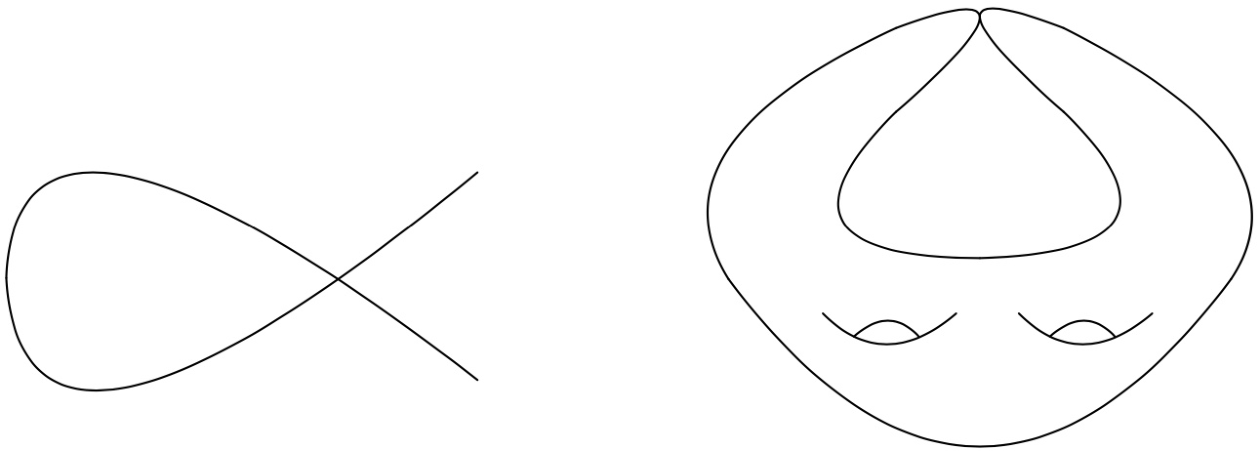
\includegraphics[width=.55\textwidth]{figures/fig-6.2.2.png}
\caption{$\mathbb C$ 上曲线的结点的代数视图 (左) 和解析视图 (右).}\label{src:6.2.2}
\end{figure}
\begin{example}\label{src:6.2.3}
\begin{enumerate}[(1)]
\item 曲线 $C=\Spec k[x,\allowbreak y]/(xy)$ 在 $0$ 处有分裂结点. 正规化 $\widetilde C\cong\mathbb A^1\coprod\mathbb A^1$ 的坐标环是 $k[x]\times k[y]$, 且 $\Gamma(C,\allowbreak \mathcal O_C)=\{(f,\allowbreak g)\in\Gamma(\widetilde C,\allowbreak \mathcal O_{\widetilde C})\mid f(0)=g(0)\}$. 换言之, $C$ 是 Ferrand 推出 (\bookref{B.4.1})
\[
\begin{tikzcd}
\Spec k\coprod\Spec k\arrow[r,"0\coprod0"]\arrow[d]&\widetilde C\arrow[d]\\
\Spec k\arrow[r,"0"']\arrow[ur,phantom,"\lrcorner",very near start]&C.
\end{tikzcd}
\]
\item 结点三次曲线 $C=\Spec k[x,\allowbreak y]/(y^2-x^2(x+1))$ 在 $0$ 处有分裂结点. 正规化 $\widetilde C\cong\mathbb A^1$ 具有坐标 $t=y/x$, 且 $x=t^2-1$, $y=t^3-t$; $C$ 同样是将 $\widetilde C$ 中 $0$ 的两个原像粘合所得的 Ferrand 推出.
\item 曲线 $C=\Spec\mathbb R[x,\allowbreak y]/(x^2+y^2)$ 在 $0$ 处有结点, 但它不是分裂结点, 因为二次型 $x^2+y^2$ 不分裂为线性因子.
\item 曲线 $\Spec\mathbb Q[x,\allowbreak y]/((x^2-2)(y^2-3))$ 在极大理想 $(x^2-2,\allowbreak y^2-3)$ 定义的点 $p$ 处有非分裂结点. 与前面结点为有理点的例子不同, $p$ 不是有理点, 域扩张 $\mathbb Q\to\kappa(p)$ 的次数为 $4$.
\item 设 $k\to\allowbreak k'$ 是次数为 $2$ 的可分域扩张, $C$ 是 $k$-代数 $\{f\in k'[x]\mid f(0)\in k\}$ 定义的 $k$ 上仿射曲线. 换言之, $C$ 是原点的包含 $0:\Spec k'\hookrightarrow\mathbb A_{k'}^1$ 沿 $\Spec k'\to\Spec k$ 的 Ferrand 推出. 曲线 $C$ 在一个 $k$-有理点处有非分裂结点.
\end{enumerate}
\end{example}
\subsection{结点的等价刻画}\label{src:6.2.2-subsection}
回顾 \S\bookref{A.3.4-subsection}, 曲线 $C$ 的奇异轨迹 $\operatorname{Sing}(C)$ 在概形意义下定义为 $\Omega_C$ 的第一个 Fitting 理想层的零点概形: 局部地, 若 $C=V(f_1,\allowbreak \ldots,\allowbreak f_m)\subseteq\mathbb A^n$, 则 $\operatorname{Sing}(C)$ 由 Jacobian 矩阵 $J=(\frac{\partial f_i}{\partial x_i})$ 的所有 $(n-1)\times(n-1)$ 子式的零点定义; 注意若 $C=V(f)\subseteq\mathbb A^2$ 是平面仿射曲线, 则 $\operatorname{Sing}(C)=V(\frac{\partial f}{\partial x},\allowbreak \frac{\partial f}{\partial y})$. 我们还将使用 \S\bookref{A.3.5-subsection} 讨论的局部完全交的性质.
\begin{proposition}[结点的刻画]\label{src:6.2.4}
设 $C$ 是域 $k$ 上的纯一维曲线, $p\in C$ 是闭点, 具有极大理想 $\mathfrak m\subseteq\mathcal O_{C,\allowbreak p}$. 以下条件等价:
\begin{enumerate}[(1)]
\item $p\in C$ 是结点;
\item $C$ 在 $p$ 处是局部完全交, 且 $\operatorname{Sing}(C)$ 在 $p\in\operatorname{Sing}(C)$ 处在 $k$ 上非分歧;
\item $k\to\kappa(p)$ 可分, $\mathcal O_{C,\allowbreak p}$ 约化, $\dim\mathfrak m/\mathfrak m^2=2$, 且存在映到 $\mathfrak m^2/\mathfrak m^3$ 中的 $0$ 的非退化二次型 $q\in\operatorname{Sym}^2\mathfrak m/\mathfrak m^2$;
\item $k\to\kappa(p)$ 可分且 $\widehat{\mathcal O}_{C,\allowbreak p}\cong\kappa(p)[[x,\allowbreak y]]/(q)$, 其中 $q$ 是非退化二次型; 且
\item 存在有限可分域扩张 $k\to\allowbreak k'$ 和点 $p'\in C_{k'}$, 使得 $\widehat{\mathcal O}_{C_{k'},\allowbreak p'}\cong k'[[x,\allowbreak y]]/(xy)$.
\end{enumerate}
\end{proposition}
\begin{proof}
假设 (1), 设 $\overline p\in C_{\overline k}$ 是 $p$ 上方的结点, $\operatorname{Sing}(C)\subseteq C$ 是概形意义的奇异轨迹. 由 Fitting 理想的性质 (见 \S\bookref{A.3.4-subsection}), $\operatorname{Sing}(C)\times_k\overline k=\operatorname{Sing}(C_{\overline k})$, 且 $\operatorname{Sing}(C_{\overline k})$ 在 $\Spec\widehat{\mathcal O}_{C_{\overline k},\allowbreak \overline p}\to\allowbreak C_{\overline k}$ 下的原像是 $\operatorname{Sing}(\Spec\widehat{\mathcal O}_{C_{\overline k},\allowbreak \overline p})$. 由于 $\widehat{\mathcal O}_{C_{\overline k},\allowbreak \overline p}\cong\overline k[[x,\allowbreak y]]/(xy)$, 有 $\operatorname{Sing}(\Spec\widehat{\mathcal O}_{C_{\overline k},\allowbreak \overline p})=V(x,\allowbreak y)=\Spec\overline k$. 因此 $\operatorname{Sing}(C)\to\Spec k$ 在 $p$ 处非分歧. 由于 $\widehat{\mathcal O}_{C_{\overline k},\allowbreak \overline p}$ 是完全交, $C$ 在 $p$ 处是局部完全交 (命题~\bookref{A.3.16}). 这得到 (2).

假设 (2), 由于 $\operatorname{Sing}(C)$ 在 $p$ 处非分歧, 域扩张 $k\to\kappa(p)$ 可分, 且 $p$ 有开邻域 $U\subseteq C$, 使得 $\operatorname{Sing}(U)=\operatorname{Sing}(C)\cap U=\{p\}$. 特别地, $\mathcal O_{C,\allowbreak p}$ 一般约化. 另一方面, 由于 $C$ 是局部完全交, $\mathcal O_{C,\allowbreak p}$ 是一维 Cohen--Macaulay 局部环, 因而没有嵌入素理想. 所以 $\mathcal O_{C,\allowbreak p}$ 约化. 利用 $C$ 是局部完全交, 可写 $\widehat{\mathcal O}_{C,\allowbreak p}=R/(f_1,\allowbreak \ldots,\allowbreak f_{n-1})$, 其中 $R$ 是正则完备局部环. 因为 $R$ 包含底域 $k$, Cohen 结构定理 (\bookref{B.5.7}) 给出 $R\cong\kappa(p)[[x_1,\allowbreak \ldots,\allowbreak x_n]]$. 由于 $\operatorname{Sing}(C)$ 在 $p$ 处非分歧, Jacobian 矩阵 $(\frac{\partial f_j}{\partial x_i})_{i,\allowbreak j}$ 的 $(n-1)\times(n-1)$ 子式生成极大理想 $\mathfrak m=(x_1,\allowbreak \ldots,\allowbreak x_n)\subseteq\widehat{\mathcal O}_{C,\allowbreak p}$. 若对某些 $i,\allowbreak j$, $\frac{\partial f_j}{\partial x_i}\in R$ 是单位, 则序列 $x_1,\allowbreak \ldots,\allowbreak \widehat{x_i},\allowbreak x_n,\allowbreak f_j$ 也生成 $\mathfrak m/\mathfrak m^2$. 可用完备 Nakayama 引理 (\bookref{B.5.6}(3)) 换坐标, 将生成元 $x_1,\allowbreak \ldots,\allowbreak x_n$ 换为 $x_1,\allowbreak \ldots,\allowbreak \widehat{x_i},\allowbreak x_n,\allowbreak f_j$. 消去 $f_j$ 后可写 $R=\kappa(p)[[x_1,\allowbreak \ldots,\allowbreak \widehat{x_i},\allowbreak x_n]]/(f_1,\allowbreak \ldots,\allowbreak \widehat{f_j},\allowbreak \ldots,\allowbreak f_{n-1})$. 有限次这样的替换后, 可假设对所有 $i,\allowbreak j$, $\frac{\partial f_j}{\partial x_i}\in\mathfrak m$. 这说明每个 $(n-1)\times(n-1)$ 子式都在 $\mathfrak m^{n-1}$ 中; 但这些子式生成 $\mathfrak m$, 故必须有 $n=2$. 因此 $\widehat{\mathcal O}_{C,\allowbreak p}=\kappa(p)[[x,\allowbreak y]]/(f)$, 其中 $f=f_2+f_3+\cdots$, 每个 $f_i$ 是 $i$ 次齐次式. 由于偏导数 $f_x,\allowbreak f_y$ 生成 $(x,\allowbreak y)$, 二次型 $q:=f_2\in\operatorname{Sym}^2\mathfrak m/\mathfrak m^2$ 必须非退化. 这得到 (3).

假设 (3), 由于 $q$ 映到 $\mathfrak m^2/\mathfrak m^3$ 中的 $0$, 对每个 $d\geq1$, 有 $\dim_{\kappa(p)}\mathfrak m^d/\mathfrak m^{d+1}=2$. 选择映到 $\mathfrak m/\mathfrak m^2$ 的一组基的元素 $x_0,\allowbreak y_0\in\mathfrak m$, 由完备 Nakayama 引理 (\bookref{B.5.6}(3)) 诱导满射 $\kappa(p)[[x,\allowbreak y]]\to\widehat{\mathcal O}_{C,\allowbreak p}$. 由于 $\mathcal O_{C,\allowbreak p}$ 约化, $\widehat{\mathcal O}_{C,\allowbreak p}$ 也约化 (命题~\bookref{3.1.21}). 由于 $\kappa(p)[[x,\allowbreak y]]$ 是 UFD, 可写成 $\kappa(p)[[x,\allowbreak y]]/(f)$, 其中 $f$ 是互异不可约元素的积, 其二次部分 $q=ax^2+bxy+cy^2$ 是非退化二次型. 我们断言可修改坐标 $x_0,\allowbreak y_0\in\mathfrak m$ 的选择, 使得 $f=q$, 即 $q(x_0,\allowbreak y_0)=0\in\widehat{\mathcal O}_{C,\allowbreak p}$. 归纳证明对每个 $N$, 存在 $x_i,\allowbreak y_i\in\mathfrak m^{i+1}$ ($i=0,\allowbreak \ldots,\allowbreak N$), 使得 $q(x_0+\cdots+x_N,\allowbreak y_0+\cdots+y_N)\in\mathfrak m^{N+3}$. 由于 $\widehat{\mathcal O}_{C,\allowbreak p}$ 完备, 这允许将 $x_0,\allowbreak y_0$ 换为 $\sum_i x_i,\allowbreak \sum_i y_i$, 得到 $\widehat{\mathcal O}_{C,\allowbreak p}\cong\kappa(p)[[x,\allowbreak y]]/(q)$. 假设已选定 $x'=x_0+\cdots+x_{N-1}$ 和 $y'=y_0+\cdots+y_{N-1}$, 则对任意 $x_N,\allowbreak y_N\in\mathfrak m^{N+1}$, 有
\[
\begin{aligned}
q(x'+x_N,y'+y_N)&=q(x',y')+(2ax_0+by_0)x_N\\
&\quad +(bx_0+2cy_0)y_N\pmod{\mathfrak m^{N+3}}.
\end{aligned}
\]
$q=ax^2+bxy+y^2$ 的非退化性说明 $2ax_0+by_0$ 与 $bx_0+2cy_0$ 线性无关. 由于 $\dim_{\kappa(p)}\mathfrak m^{N+2}/\mathfrak m^{N+3}=2$, 可选择 $x_N,\allowbreak y_N$, 使得 $q(x'+x_N,\allowbreak y'+y_N)\in\mathfrak m^{N+3}$. 这完成 (4).

假设 (4), 利用 $q$ 非退化, 可选择次数为 $2$ 的可分域扩张 $\kappa(p)\to\allowbreak k'$, 使 $q$ 分裂为线性形式的积. 因而 $\widehat{\mathcal O}_{C,\allowbreak p}\otimes_k k'\cong k'[[x,\allowbreak y]]/(xy)$, 得到 (5). 最后, (5) 蕴含 $p$ 是结点. 另见~\cite[Tags 0C49, 0C4D 和 0C4E]{SP}.
\end{proof}
\begin{exercise}[容易]\label{src:6.2.5}
证明 $\Spec k[x,\allowbreak y]/(f)$ 在 $0$ 处有结点当且仅当 $f(0)=f_x(0)=f_y(0)=0$, 且
\[
\det\begin{pmatrix}f_{xx}(0)&f_{xy}(0)\\f_{yx}(0)&f_{yy}(0)\end{pmatrix}\neq0.
\]
\end{exercise}
\begin{exercise}[很好的练习]\label{src:6.2.6}
设 $C$ 是域 $k$ 上的纯一维约化曲线, 正规化为 $\pi:\widetilde C\to\allowbreak C$. 证明 $p\in C$ 是结点当且仅当 $k\to\kappa(p)$ 可分, $\dim_{\kappa(p)}(\pi_*\mathcal O_{\widetilde C}/\mathcal O_C)\otimes\kappa(p)=1$, 且 $\sum_{\pi(q)=p}[\kappa(q):\kappa(p)]=2$.

\textit{提示:} 利用正规化与完备化交换 (见注记~\bookref{3.1.25}), 将 $(\pi_*\mathcal O_{\widetilde C}/\mathcal O_C)\otimes\kappa(p)$ 等同于商 $\widetilde A/A$, 其中 $A=\widehat{\mathcal O}_{C,\allowbreak p}$, $\widetilde A$ 是其正规化. 为证明 ($\Leftarrow$), 利用 $\widetilde A$ 是完备 DVR 的积, 推导 $A$ 的结构. 另见~\cite[Tag 0C4A]{SP}.
\end{exercise}
\begin{remark}\label{src:6.2.7}
量 $\dim_{\kappa(p)}(\pi_*\mathcal O_{\widetilde C}/\mathcal O_C)\otimes\kappa(p)$ 称为 $p$ 的\newterm{$\delta$-不变量}{delta invariant}, 和 $\sum_{\pi(q)=p}[\kappa(q):\kappa(p)]_{\mathrm{sep}}$ 称为 $p$ 上方的\textit{几何分支数}. 尖点 $k[x,\allowbreak y]/(y^2-x^3)$ 的 $\delta$-不变量为 $1$, 但只有一个几何分支.
\end{remark}
\newpage
\begin{proposition}[结点的局部结构]\label{src:6.2.8}
设 $C$ 是域 $k$ 上的曲线. 若 $p\in C$ 是结点, 则存在有限可分域扩张 $k\to\allowbreak k'$ 和平展邻域
\begin{equation}\label{src:6.2.9}
\begin{tikzcd}[column sep=small]
&(U,u)\arrow[dl]\arrow[dr]&\\
(C,p)&&(\Spec k'[x,y]/(xy),0).
\end{tikzcd}
\end{equation}
\end{proposition}
\begin{proof}
由结点的刻画 (\bookref{6.2.4}(5)), 存在有限可分域扩张 $k\to\allowbreak k'$, 使得 $\widehat{\mathcal O}_{C,\allowbreak p}\otimes_k k'\cong k'[[x,\allowbreak y]]/(xy)$. 结论现在是 Artin 逼近 (\bookref{B.5.21}) 的推论.
\end{proof}
不久将把它推广到结点曲线族 (定理~\bookref{6.2.26}).
\begin{example}\label{src:6.2.10}
我们为结点三次曲线 $C=\Spec\mathbb C[x,\allowbreak y]/(y^2-x^2(x-1))$ 构造明确的平展邻域. 事实上, 例~\bookref{1.5.4} 中已基本说明如何做到: 加入平方根 $t=\sqrt{x-1}$ 后, $y^2-x^3+x^2=(y-xt)(y+xt)$. 因此可取 $(x,\allowbreak y,\allowbreak t)\mapsto(x,\allowbreak y)$ 给出的初等平展邻域 $U=\Spec\mathbb C[x,\allowbreak y,\allowbreak t]_t/(y^2-x^3+x^2,\allowbreak t^2-x+1)\to\allowbreak C$, 以及由 $(x,\allowbreak y,\allowbreak t)\mapsto(y-xt,\allowbreak y+xt)$ 定义的平展邻域 $U\to\Spec\mathbb C[x,\allowbreak y]/(xy)$.
\end{example}
\begin{exercise}\label{src:6.2.11}
给出不使用 Artin 逼近的结点局部结构 (\bookref{6.2.8}) 的证明.

\textit{提示:} 利用严格 Hensel 化 $\mathcal O_{C,\allowbreak p}^{\mathrm{sh}}$ 的正规化有两个分支, 找到仿射平展邻域 $(\Spec R,\allowbreak u)\to(C,\allowbreak p)$, 使得 $\widetilde R=R_1\times R_2$. 利用正合列 $0\to\allowbreak R\to\allowbreak R_1\times R_2\to\kappa(u)\to0$, 构造映到 $(1,\allowbreak 0),\allowbreak (0,\allowbreak 1)\in R_1\times R_2$ 的元素 $x,\allowbreak y\in R$, 并说明 $\kappa(u)[x,\allowbreak y]/(xy)\to\allowbreak R$ 平展.
\end{exercise}
\subsection{亏格公式}\label{src:6.2.3-subsection}
\begin{proposition}[亏格公式]\label{src:6.2.12}
设 $C$ 是代数闭域 $k$ 上的连通结点射影曲线, 具有 $\delta$ 个结点和 $\nu$ 个不可约分支. 设 $C=\bigcup_i C_i$ 是不可约分解, $\widetilde C_i$ 是 $C_i$ 的正规化, 其亏格为 $g(\widetilde C_i)$. $C$ 的亏格 $g$ 满足
\[
g=\sum_{i=1}^{\nu}g(\widetilde C_i)+\delta-\nu+1.
\]
\end{proposition}
\begin{proof}
设 $p_1,\allowbreak \ldots,\allowbreak p_\delta\in C$ 是 $C$ 的结点. 我们断言正规化 $\pi:\widetilde C\to\allowbreak C$ 诱导短正合列
\[
0\to\mathcal O_C\to\pi_*\mathcal O_{\widetilde C}\to\bigoplus_{j=1}^{\delta}\kappa(p_j)\to0.
\]
只需在结点 $p_i\in C$ 附近平展局部地验证; 由结点的局部结构 (\bookref{6.2.8}), 可假设 $C=\Spec k[x,\allowbreak y]/(xy)$. 此时 $\widetilde C=\Spec(k[x]\times k[y])$, 上述序列对应于 $0\to\allowbreak k[x,\allowbreak y]/(xy)\to\allowbreak k[x]\times k[y]\to\allowbreak k\to0$. 也可利用正规化与完备化交换; 如上直接计算可知, 若 $A:=\widehat{\mathcal O}_{C,\allowbreak p}\cong k[[x,\allowbreak y]]/(xy)$, 则 $\widetilde A/A\cong k$.

短正合列诱导上同调长正合列
\[
\begin{aligned}
0&\to\underbrace{\mathrm H^0(C,\mathcal O_C)}_1\to\underbrace{\mathrm H^0(\widetilde C,\mathcal O_{\widetilde C})}_{\nu}\to\underbrace{\bigoplus_j\kappa(p_j)}_{\delta}\\
&\to\underbrace{\mathrm H^1(C,\mathcal O_C)}_g\to\underbrace{\mathrm H^1(\widetilde C,\mathcal O_{\widetilde C})}_{\sum_i g(\widetilde C_i)}\to0,
\end{aligned}
\]
其中标注表示维数. 由此得到结论.
\end{proof}
\begin{figure}[H]
\centering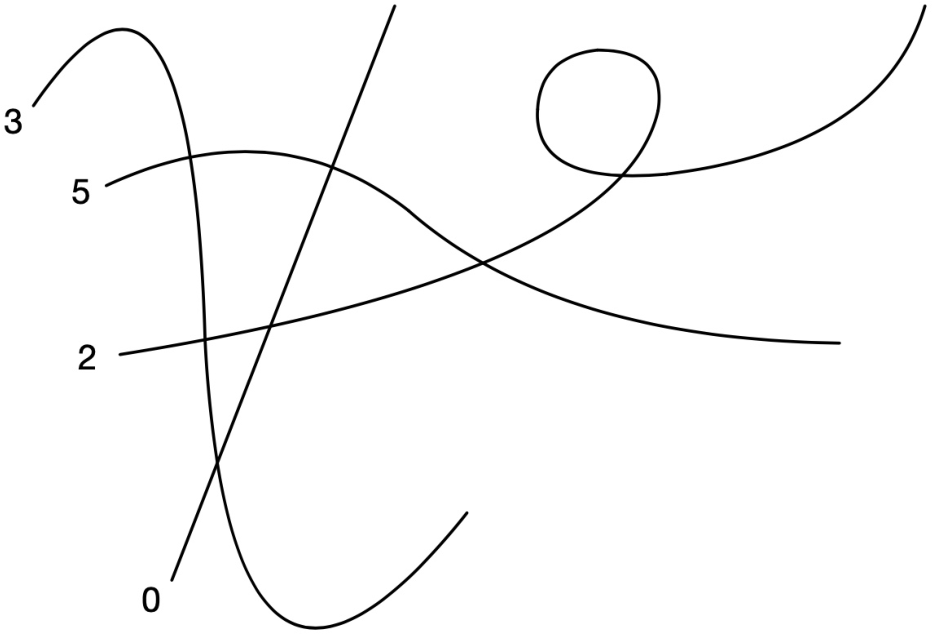
\includegraphics[width=.43\textwidth]{figures/fig-6.2.13.png}
\caption{亏格为 $14$ 的结点曲线的一个例子.}\label{src:6.2.13}
\end{figure}
\begin{remark}\label{src:6.2.14}
注意 $\delta-\nu+1$ 恰为曲线 $C$ 围出的有界连通区域数, 如图~\bookref{6.2.13} 所示. 因而可从图中方便地计算结点曲线的亏格: 将不可约分支的几何亏格相加, 再加上有界区域数. 定义~\bookref{6.3.9} 给出用对偶图作出的另一种解释. 对非结点曲线, 有类似的亏格公式, 涉及奇点的 $\delta$-不变量 (见注记~\bookref{6.2.7}).
\end{remark}
\subsection{对偶化层}\label{src:6.2.4-subsection}
由于域 $k$ 上的结点曲线 $C$ 是局部完全交, $C$ 是 Gorenstein 的, 存在对偶化线丛 $\omega_C$, 带有迹映射 $\operatorname{tr}_C:\mathrm H^1(C,\allowbreak \omega_C)\xrightarrow{\sim}k$; 见~\cite[III.7.11]{Har77} 或~\cite[\S IV]{Ser88}. 换言之, 对每个凝聚层 $F$, 自然配对
\[
\operatorname{Hom}_{\mathcal O_C}(F,\omega_C)\times\mathrm H^1(C,F)\to\mathrm H^1(C,\omega_C)\xrightarrow{\operatorname{tr}}k
\]
完美. 鉴于它对研究稳定曲线的重要性, 以下在代数闭域 $k$ 上给出 $\omega_C$ 的明确描述. 设 $\Sigma:=C^{\mathrm{sing}}$ 是奇异轨迹, $U=C\setminus\Sigma$. 设 $\pi:\widetilde C\to\allowbreak C$ 是正规化, $\widetilde\Sigma,\allowbreak \widetilde U$ 是 $\Sigma,\allowbreak U$ 的原像, 如下图:
\begin{equation}\label{src:6.2.15}
\begin{tikzcd}
\widetilde U\arrow[r,hook]\arrow[d,"\sim"']&\widetilde C\arrow[d,"\pi"]&\widetilde\Sigma\arrow[l,hook']\arrow[d]\\
\widetilde U\arrow[r,hook]&C&\Sigma.\arrow[l,hook']
\end{tikzcd}
\end{equation}
将这些点排序为 $\Sigma=\{z_1,\allowbreak \ldots,\allowbreak z_n\}$, 设 $\pi^{-1}(z_i)=\{p_i,\allowbreak q_i\}$. 由于 $\widetilde C$ 光滑, 微分层 $\Omega_{\widetilde C}$ 是对偶化线丛. 有短正合列
\begin{equation}\label{src:6.2.16}
0\to\Omega_{\widetilde C}\to\Omega_{\widetilde C}(\widetilde\Sigma)\to\mathcal O_{\widetilde\Sigma}\to0,
\end{equation}
由序列 $0\to\mathcal O_{\widetilde C}(-\widetilde\Sigma)\to\mathcal O_{\widetilde C}\to\mathcal O_{\widetilde\Sigma}\to0$ 张量 $\Omega_{\widetilde C}(\widetilde\Sigma)$ 得到. 因为 $\Omega_{\widetilde C}(\widetilde\Sigma)|_{\widetilde U}=\Omega_{\widetilde U}$, 可将 $\Omega_{\widetilde C}(\widetilde\Sigma)$ 的截面解释为 $\Omega_{\widetilde C}$ 的有理截面, 在 $\widetilde\Sigma$ 上至多有一阶极点. 在开集 $\widetilde V\subseteq\widetilde C$ 上取~\bookeqref{6.2.16} 的截面得到
\begin{equation}\label{src:6.2.17}
\begin{aligned}
0\to\Gamma(\widetilde V,\Omega_{\widetilde C})\to\Gamma(\widetilde V,\Omega_{\widetilde C}(\widetilde\Sigma))&\to\bigoplus_{y\in\widetilde V\cap\widetilde\Sigma}\kappa(y),\\
s&\mapsto(\operatorname{res}_y(s)),
\end{aligned}
\end{equation}
最后一个映射将有理截面 $s\in\Gamma(\widetilde V\cap\widetilde U,\allowbreak \Omega_{\widetilde C})$ 映到一个元组, 其在 $y\in\widetilde V\cap\widetilde\Sigma$ 处的坐标是 $s$ 在 $y$ 处的留数 $\operatorname{res}_y(s)$.
\begin{definition}[对偶化层]\label{src:6.2.18}
设 $C$ 是代数闭域 $k$ 上的结点曲线. 用~\bookeqref{6.2.15} 和~\bookeqref{6.2.17} 的记号, 定义子层 $\omega_C\subseteq\pi_*\Omega_{\widetilde C}(\widetilde\Sigma)$ 如下: 在 $V\subseteq C$ 上的截面是 $\Omega_{\widetilde C}$ 在 $\pi^{-1}(V)$ 上的有理截面 $s$, 在 $\widetilde\Sigma$ 上至多有一阶极点, 且对每个结点 $z_i\in V\cap\Sigma$ 及其原像 $p_i,\allowbreak q_i\in\pi^{-1}(V)$, 有 $\operatorname{res}_{p_i}(s)+\operatorname{res}_{q_i}(s)=0$.
\end{definition}
由定义, $\omega_C$ 位于以下两个正合列中:
\[
\begin{aligned}
0\to\omega_C\to\pi_*\Omega_{\widetilde C}(\widetilde\Sigma)&\to\bigoplus_{z_i\in\Sigma}k\to0,\\
s&\mapsto(\operatorname{res}_{p_i}(s)+\operatorname{res}_{q_i}(s)).
\end{aligned}
\]
\[
\begin{aligned}
0\to\pi_*\Omega_{\widetilde C}\to\omega_C&\to\bigoplus_{z_i\in\Sigma}k\to0,\\
s&\mapsto(\operatorname{res}_{p_i}(s)).
\end{aligned}
\]
\begin{example}[局部计算]\label{src:6.2.19}
设 $C=\Spec k[x,\allowbreak y]/(xy)$. 则 $\widetilde C=\mathbb A^1\coprod\mathbb A^1$, 分别具有坐标 $x,\allowbreak y$. $C$ 的奇异轨迹是 $\Sigma=\{0\}$, 原像 $\widetilde\Sigma$ 由两个原点组成. 此时 $\Gamma(\widetilde C,\allowbreak \Omega_{\widetilde C})=\Gamma(\mathbb A^1,\allowbreak \Omega_{\mathbb A^1})\times\Gamma(\mathbb A^1,\allowbreak \Omega_{\mathbb A^1})$, $(\frac{dx}{x},\allowbreak -\frac{dy}{y})$ 是 $\Omega_{\widetilde C}$ 的有理截面, 在 $p,\allowbreak q$ 处留数相反. 事实上, $\Gamma(C,\allowbreak \omega_C)$ 的每个截面形如
\[
\left(f(x)\frac{dx}{x},g(y)\frac{-dy}{y}\right)=\bigl(f(x)+g(y)-f(0)\bigr)\cdot\left(\frac{dx}{x},\frac{-dy}{y}\right),
\]
其中多项式 $f(x),\allowbreak g(y)$ 满足 $f(0)=g(0)$; 这正是 $(f,\allowbreak g)\in\Gamma(\widetilde C,\allowbreak \mathcal O_{\widetilde C})$ 下降为整体函数 $f(x)+g(y)-f(0)\in\Gamma(C,\allowbreak \mathcal O_C)$ 的条件. 换言之, $\omega_C\cong\mathcal O_C$, 生成元为 $(\frac{dx}{x},\allowbreak -\frac{dy}{y})$.
\end{example}
\begin{example}\label{src:6.2.20}
设 $C$ 是射影平面结点三次曲线, $\mathbb P^1\to\allowbreak C$ 是正规化, 坐标为 $[x:y]$, 使得 $0,\allowbreak \infty$ 是结点的纤维. $\mathbb P^1$ 上的有理微分 $\eta:=\frac{dx}{x}=-\frac{dy}{y}$ 满足 $\operatorname{res}_0\eta+\operatorname{res}_{\infty}\eta=0$. 不难看出 $\omega_C$ 的每个局部截面均为 $\eta$ 的倍数; 换言之, $\omega_C\cong\mathcal O_C$, 生成元为 $\eta$.
\end{example}
\begin{exercise}[细节]\label{src:6.2.21}
设 $C$ 是代数闭域 $k$ 上的连通结点射影曲线. 暂时如定义~\bookref{6.2.18} 定义子层
\[
K_C=\ker\left(\pi_*\Omega_{\widetilde C}(\widetilde\Sigma)\to\bigoplus_{z_i\in\Sigma}k\right).
\]
\begin{enumerate}[(a)]
\item 证明若 $\pi:C'\to\allowbreak C$ 是平展态射, 则 $\pi^*K_C\cong K_{C'}$.

\textit{提示:} 利用正规化与平展基变换交换.
\item 证明 $K_C$ 是线丛.

\textit{提示:} 用结点的局部结构 (\bookref{6.2.8}) 和例~\bookref{6.2.19} 中的局部计算.
\item (困难) 证明 $K_C$ 是对偶化层.

\textit{提示:} 利用正规化归结到光滑曲线的情形:
\begin{enumerate}[(i)]
\item 用 Yoneda 引理证明, 只需给出函子 $\operatorname{Pic}(C)\to\operatorname{Vect}_k$ 的同构 $\operatorname{Hom}_{\mathcal O_C}(-,\allowbreak K_C)\cong\mathrm H^1(C,\allowbreak -)^\vee$.
\item 对任意 $L\in\operatorname{Pic}(C)$, 证明将定义 $K_C$ 的正合列张量 $L^\vee$ 并取上同调, 得到等同
\[
\begin{aligned}
\operatorname{Hom}_{\mathcal O_C}(L,K_C)&\cong\mathrm H^0(C,L^\vee\otimes K_C)\\
&\cong\ker\left(\mathrm H^0(\widetilde C,\pi^*L^\vee\otimes\Omega_{\widetilde C}(\widetilde\Sigma))\to\bigoplus_{z_i\in\Sigma}k\right).
\end{aligned}
\]
\item 用短正合列 $0\to\pi_*\pi^*(L(\widetilde\Sigma))\to\allowbreak L\to\bigoplus_{z_i\in\Sigma}k\to0$, 推出
\[
\mathrm H^1(C,L)^\vee=\ker\left(\mathrm H^1(\widetilde C,\pi^*L(\widetilde\Sigma))^\vee\to\bigoplus_{z_i\in\Sigma}k\right).
\]
\item 证明 $\widetilde C$ 上的 Serre 对偶给出的同构 $\mathrm H^0(\widetilde C,\allowbreak \pi^*L^\vee\otimes\Omega_{\widetilde C}(\widetilde\Sigma))\cong\mathrm H^1(\widetilde C,\allowbreak \pi^*L(\widetilde\Sigma))^\vee$ 与到 $\bigoplus_{z_i\in\Sigma}k$ 的两个映射交换.
\end{enumerate}
另见~\cite[命题 13.2.9]{Ols16}. 其他方法见~\cite[第四章 \S 3]{Ser88}, \cite[引理 10.3.12]{Liu02} 和~\cite[第十章 \S 2]{ACG11}.
\item 若 $T\subseteq C$ 是子曲线, 补曲线为 $T^c:=\overline{C\setminus T}$, 证明
\[
\omega_C|_T=\omega_T(T\cap T^c).
\]
\end{enumerate}
\end{exercise}
\newpage
\begin{exercise}[很好的练习]\label{src:6.2.22}
设 $C$ 是代数闭域 $k$ 上的连通结点射影曲线. 设 $\pi:\widetilde C\to\allowbreak C$ 是正规化, $\widetilde\Sigma\subseteq\widetilde C$ 是结点原像的集合. 证明有等同
\[
\pi_*\mathcal H om_{\mathcal O_{\widetilde C}}(\Omega_{\widetilde C}(\widetilde\Sigma),\mathcal O_{\widetilde C})\cong\mathcal H om_{\mathcal O_C}(\Omega_C,\mathcal O_C),
\]
或等价地, $\pi_*(T_{\widetilde C}(-\widetilde\Sigma))=T_C$. 换言之, $C$ 上的正则向量场对应于 $\widetilde C$ 上在结点原像处为零的正则向量场.
\end{exercise}
\begin{remark}\label{src:6.2.23}
上述对偶化层 $\omega_C$ 的明确描述可推广到任意约化 Gorenstein 曲线 $C$. $\omega_C$ 的截面有时称为\newterm{Rosenlicht 微分}{Rosenlicht differentials}. 见~\cite[命题 6.2]{BHPV04} 和~\cite[第四章]{Ser88}.
\end{remark}
\subsection{结点曲线族}\label{src:6.2.5-subsection}
回顾, 具有一维纤维的态射 $C\to\allowbreak S$ 的相对奇异轨迹 $\operatorname{Sing}(C/S)$ 由 $\Omega_{C/S}$ 的第一个 Fitting 理想层定义; 见定义~\bookref{A.3.14}. syntomic 态射是纤维为局部完全交的 fppf 态射 (即平坦且局部有限表现); 见 \S\bookref{A.3.5-subsection}.
\begin{proposition}\label{src:6.2.24}
设 $C\to\allowbreak S$ 是概形的 fppf 态射, $s\in S$ 是点, 纤维 $C_s$ 纯一维. 点 $p\in C_s$ 是结点当且仅当 $C\to\allowbreak S$ 在 $p$ 处 syntomic, 且相对奇异轨迹 $\operatorname{Sing}(C/S)\to\allowbreak S$ 在 $p$ 处非分歧.
\end{proposition}
\begin{proof}
$C\to\allowbreak S$ 在 $p$ 处 syntomic 及 $\operatorname{Sing}(C)\to\allowbreak S$ 在 $p$ 处非分歧这两个条件, 都是关于 $s$ 上方纤维的条件. 由于 $\operatorname{Sing}(C/S)_s=\operatorname{Sing}(C_s)$, 结论由结点的刻画 (\bookref{6.2.4}) 中 (1) $\Leftrightarrow$ (4) 的等价性得到.
\end{proof}
上述刻画说明结点曲线族这一性质沿极限下降 (定义~\bookref{B.3.6}).
\begin{lemma}\label{src:6.2.25}
概形态射的以下性质沿极限下降: 每个纤维都是纯一维结点曲线的 fppf 态射.
\end{lemma}
\begin{proof}
由态射性质沿极限的下降 (\bookref{B.3.7}), 已知 fppf, syntomic, 非分歧及具有连通纯一维纤维这些性质沿极限下降. 由于相对奇异轨迹与基变换交换, 结论由命题~\bookref{6.2.24} 得到.
\end{proof}
\subsection{结点曲线族的局部结构}\label{src:6.2.6-subsection}
由光滑态射的局部结构 (\bookref{A.3.4}), 若 $C\to\allowbreak S$ 是光滑曲线族, 则 $s\in S$ 上方的每个点 $p\in C$ 平展局部地同构于相对一维仿射空间. 更准确地, 有交换图
\[
\begin{tikzcd}[column sep=small]
(C,p)\arrow[d]&(C',p')\arrow[l,"\mathrm{op}"']\arrow[r,"\text{ét}"]\arrow[d]&(S'\times_{\mathbb Z}\mathbb A^1_{\mathbb Z},(s',0))\arrow[dl]\\
(S,s)&(S',s')\arrow[l,"\mathrm{op}"']&
\end{tikzcd}
\]
其中左侧水平映射是开浸入, 右侧映射平展, 且 $S'\times_{\mathbb Z}\mathbb A^1_{\mathbb Z}=\mathbb A^1_{S'}\to\allowbreak S'$ 是 $\mathbb A^1_{\mathbb Z}\to\Spec\mathbb Z$ 的基变换. 我们为结点曲线族建立类似的局部结构, 给出结点局部结构 (\bookref{6.2.8}) 的相对版本.
\begin{theorem}[结点曲线族的局部结构]\label{src:6.2.26}
设 $\pi:C\to\allowbreak S$ 是 fppf 态射, 每个几何纤维都是曲线. 设 $p\in C$ 是点 $s\in S$ 上方纤维 $C_s$ 中的结点. 有交换图
\begin{equation}\label{src:6.2.27}
\begin{tikzcd}[column sep=small]
(C,p)\arrow[d]&(C',p')\arrow[l,"\text{ét}"']\arrow[r,"\text{ét}"]\arrow[d]&(\Spec A[x,y]/(xy-f),(s',0))\arrow[dl]\\
(S,s)&(\Spec A,s')\arrow[l,"\text{ét}"']&
\end{tikzcd}
\end{equation}
其中每个水平映射平展, $f\in A$ 是在 $s'$ 处为零的函数.
\end{theorem}
\newpage
\begin{remark}\label{src:6.2.28}
换言之, 每个结点曲线族在源与靶上平展局部地具有由函数 $f\in A$ 诱导的纤维积中的上方水平箭头的结构:
\[
\begin{tikzcd}
\Spec A[x,y]/(xy-f)\arrow[r]\arrow[d]&\Spec A\arrow[d,"f"]\\
\Spec\mathbb Z[x,y,t]/(xy-t)\arrow[r]&\Spec\mathbb Z[t].
\end{tikzcd}
\]
\end{remark}
\begin{proof}
我们给出从局部到整体的证明.

\textit{步骤 1: 归结到 $S$ 在 $\mathbb Z$ 上有限型的情形.} 用极限方法和引理~\bookref{6.2.25}.

\textit{步骤 2: 归结到 $\widehat{\mathcal O}_{C_s,\allowbreak p}\cong\kappa(s)[[x,\allowbreak y]]/(xy)$ 的情形.} 由命题~\bookref{6.2.4}, 存在有限可分域扩张 $\kappa(s)\to\allowbreak k'$ 和点 $p'\in C_s\times_{\kappa(s)}k'$, 其完备化同构于 $k'[[x,\allowbreak y]]/(xy)$. 取平展态射 $(S',\allowbreak s')\to(S,\allowbreak s)$, 使得在 $\kappa(s)$ 上有 $\kappa(s')\cong k'$, 并将 $S$ 换为 $S'$.

\textit{步骤 3: 证明对某个函数 $\widehat f\in\widehat{\mathfrak m}_s\subseteq\widehat{\mathcal O}_{S,\allowbreak s}$, 有 $\widehat{\mathcal O}_{C,\allowbreak p}\cong\widehat{\mathcal O}_{S,\allowbreak s}[[x,\allowbreak y]]/(xy-\widehat f)$.} 我们断言存在元素 $\widehat x,\allowbreak \widehat y\in\widehat{\mathcal O}_{C,\allowbreak p}$ 和 $\widehat f\in\widehat{\mathfrak m}_s\subseteq\widehat{\mathcal O}_{S,\allowbreak s}$, 满足 $\widehat x\widehat y-\widehat f=0$. 为此, 归纳构造 $n\geq0$ 时的元素 $x_n,\allowbreak y_n\in\widehat{\mathcal O}_{C,\allowbreak p}$ 和 $f_n\in\widehat{\mathfrak m}_s$, 它们相容 (即 $x_{n+1}\equiv x_n\pmod{\mathfrak m^{n+1}}$ 等), 且
\begin{equation}\label{src:6.2.29}
x_ny_n-f_n\in\widehat{\mathfrak m}_s^{n+1}\widehat{\mathcal O}_{C,p}.
\end{equation}
定义 $\widehat x=\lim_n x_n$, $\widehat y=\lim_n y_n$, $\widehat f=\lim_n f_n$, 即得断言.

初始情形 $n=0$ 由步骤 2 处理: 设 $\overline x,\allowbreak \overline y\in\widehat{\mathcal O}_{C_s,\allowbreak p}$ 是 $x,\allowbreak y$ 在同构 $\widehat{\mathcal O}_{C_s,\allowbreak p}\cong\kappa(s)[[x,\allowbreak y]]/(xy)$ 下的像, 取 $x_0,\allowbreak y_0\in\widehat{\mathcal O}_{C,\allowbreak p}$ 为它们在满射 $\widehat{\mathcal O}_{C,\allowbreak p}\to\widehat{\mathcal O}_{C_s,\allowbreak p}$ 下的任意提升, 并令 $f_0=0$. 假设已构造满足~\bookeqref{6.2.29} 的 $x_n,\allowbreak y_n,\allowbreak f_n$, 写成
\[
x_ny_n-f_n=\sum_i a_i b_i,\qquad a_i\in\widehat{\mathfrak m}_s^{n+1},\quad b_i\in\widehat{\mathcal O}_{C,p}.
\]
由于 $x_n,\allowbreak y_n$ 生成 $p$ 在纤维 $C_s$ 中的极大理想, 可利用剩余域上的等式 $\kappa(s)=\kappa(p)$, 找到 $a'_i\in\widehat{\mathcal O}_{S,\allowbreak s}$ 和 $b'_i,\allowbreak b''_i\in\widehat{\mathcal O}_{C,\allowbreak p}$, 使得
\[
b_i-(x_nb'_i+y_nb''_i+a'_i)\in\widehat{\mathfrak m}_s\widehat{\mathcal O}_{C,p}.
\]
然后定义
\[
x_{n+1}=x_n-\sum_i a_i b''_i,\quad y_{n+1}=y_n-\sum_i a_i b'_i,\quad f_{n+1}=f_n+\sum_i a_i a'_i,
\]
并验证
\[
\begin{aligned}
x_{n+1}y_{n+1}-f_{n+1}
&=(x_n-\sum_i a_i b''_i)(y_n-\sum_i a_i b'_i)-(f_n+\sum_i a_i a'_i)\\
&=(x_ny_n-f_n)-x_n\sum_i a_i b'_i-y_n\sum_i a_i b''_i-\sum_i a_i a'_i+\sum_{i,j}a_i a_j b''_i b'_j\\
&=\sum_i a_i b_i-x_n\sum_i a_i b'_i-y_n\sum_i a_i b''_i-\sum_i a_i a'_i+\sum_{i,j}a_i a_j b''_i b'_j\\
&=\sum_i\underbrace{a_i}_{\widehat{\mathfrak m}_s^{n+1}}\underbrace{(b_i-x_nb'_i-y_nb''_i-a'_i)}_{\widehat{\mathfrak m}_s\widehat{\mathcal O}_{C,p}}+\sum_{i,j}\underbrace{a_i a_j}_{\widehat{\mathfrak m}_s^{2(n+1)}}b''_i b'_j
\end{aligned}
\]
属于 $\widehat{\mathfrak m}_s^{n+2}\widehat{\mathcal O}_{C,\allowbreak p}$.

建立断言后, 有良定义的 $\mathcal O_{S,\allowbreak s}$-代数同态
\[
\widehat{\mathcal O}_{S,s}[[x,y]]/(xy-\widehat f)\to\widehat{\mathcal O}_{C,p},
\]
由 $x\mapsto\widehat x$, $y\mapsto\widehat y$ 定义. 模 $\widehat{\mathfrak m}_s$ 后它满射, 所以由完备 Nakayama 引理 (\bookref{B.5.6}(2)) 满射; 由平坦性局部判据的一个版本 (引理~\bookref{A.2.8}) 单射, 因而是同构.

\textit{步骤 4 (从形式邻域到平展邻域): 将步骤 3 中形式邻域的同构延伸到平展邻域.} 由步骤 3, 有图
\[
\begin{tikzcd}[column sep=small]
C\times_S\Spec\widehat{\mathcal O}_{S,s}\arrow[dr]&&\Spec\widehat{\mathcal O}_{S,s}[x,y]/(xy-\widehat f)\arrow[dl]\\
&\Spec\widehat{\mathcal O}_{S,s}&
\end{tikzcd}
\]
其中点 $(p,\allowbreak s)\in C\times_S\Spec\widehat{\mathcal O}_{S,\allowbreak s}$ 和 $(s,\allowbreak 0)\in\Spec\widehat{\mathcal O}_{S,\allowbreak s}[x,\allowbreak y]/(xy-\widehat f)$ 的完备化同构. Artin 逼近 (\bookref{B.5.21}) 的一个推论说明存在定义在 $\Spec\widehat{\mathcal O}_{S,\allowbreak s}$ 上的平展态射
\begin{equation}\label{src:6.2.30}
\begin{tikzcd}[column sep=small]
&(U,u)\arrow[dl]\arrow[dr]&\\
(C\times_S\Spec\widehat{\mathcal O}_{S,s},(p,s))&&(\Spec\widehat{\mathcal O}_{S,s}[x,y]/(xy-\widehat f),(s,0)).
\end{tikzcd}
\end{equation}
将 $S$ 换为 $s$ 的仿射开邻域后, 可假设 $S=\Spec A$ 仿射. 由 Néron--Popescu (\bookref{B.5.15}), 可将 $\widehat{\mathcal O}_{S,\allowbreak s}=\operatorname{colim}B_\lambda$ 写成光滑 $A$-代数的有向余极限. 置 $S_\lambda=\Spec B_\lambda$, $C_\lambda=C\times_S S_\lambda$, $U_\lambda=U\times_S S_\lambda$. 对 $\lambda\gg0$, $\widehat f\in\widehat{\mathcal O}_{S,\allowbreak s}$ 是某个元素 $f_\lambda\in B_\lambda$ 的像, $x,\allowbreak y$ 在 $\Gamma(U,\allowbreak \mathcal O_U)$ 中的拉回是 $\Gamma(U_\lambda,\allowbreak \mathcal O_{U_\lambda})$ 中元素在 $U\to\allowbreak U_\lambda$ 下的拉回. 这给出 $S_\lambda$ 上的交换图
\[
\begin{tikzcd}[column sep=small]
&U_\lambda\arrow[dl]\arrow[dr]&\\
C_\lambda&&\Spec B_\lambda[x,y]/(xy-f_\lambda),
\end{tikzcd}
\]
沿 $\Spec\widehat{\mathcal O}_{S,\allowbreak s}\to\allowbreak S_\lambda$ 基变换后成为~\bookeqref{6.2.30}. 由态射性质沿极限的下降 (\bookref{B.3.7}), 平展性沿极限下降, 所以对 $\lambda\gg0$, 映射 $U_\lambda\to\allowbreak C_\lambda$ 和 $U_\lambda\to\Spec B_\lambda[x,\allowbreak y]/(xy-f_\lambda)$ 平展. 令 $u_\lambda=(u,\allowbreak s_\lambda)\in U_\lambda$, 得到交换图
\[
\begin{tikzcd}[column sep=small]
(C,p)\arrow[d]&(U_\lambda,u_\lambda)\arrow[l,"\mathrm{sm}"']\arrow[r,"\text{ét}"]\arrow[d]&(\Spec B_\lambda[x,y]/(xy-f_\lambda),(s_\lambda,0))\arrow[dl]\\
(S,s)&(\Spec B_\lambda,s_\lambda)\arrow[l,"\mathrm{sm}"']&
\end{tikzcd}
\]
这就是所需的图~\bookeqref{6.2.27}, 但左侧水平箭头光滑而非平展. 由于光滑映射平展局部地有截面 (推论~\bookref{A.3.5}), 存在平展映射 $(\Spec A,\allowbreak s')\to(S,\allowbreak s)$ 和 $S$ 上的映射 $(\Spec A,\allowbreak s')\to(S_\lambda,\allowbreak s_\lambda)$. 令 $C':=U_\lambda\times_{S_\lambda}\Spec A$, $p'=(u_\lambda,\allowbreak s')$, 即得结论. 另见~\cite[Tag 0CBY]{SP}.
\end{proof}
\begin{exercise}\label{src:6.2.31}
按以下方式给出避免 Artin 逼近和 Néron--Popescu 的另一证明:
\begin{enumerate}[(i)]
\item 归结到 $S$ 在 $\mathbb Z$ 上有限型的情形.
\item 归结到 $C\to\allowbreak S$ 是仿射概形的 syntomic 态射的情形, 其几何纤维连通且至多有两个不可约分支, $\operatorname{Sing}(C/S)\to\allowbreak S$ 是同构或由非零因子定义的闭浸入.
\item 利用正规化和 Hensel 化的性质, 处理 $\operatorname{Sing}(C/S)=S$ 与 $\operatorname{Sing}(C/S)=V(f)$ 两种情形.
\end{enumerate}
\end{exercise}

% Source printed pp. 225-235 / PDF pp. 233-243.
\section{稳定曲线}\label{src:6.3}
\begin{epigraph}
唯一的问题是巧妙地选择``边界''分支, 即决定允许哪些非一般的簇.
\epigraphauthor{Alan Mayer 和 David Mumford~\cite[3 页]{MM64a}}
\end{epigraph}
Mayer 和 Mumford 在~\cite{MM64a,MM64b} 中引入稳定曲线, 为 $M_g$ 给出具有模意义的紧化, 其中边界 $\overline M_g\setminus M_g$ 上的点对应于奇异稳定曲线.
\subsection{定义与等价条件}\label{src:6.3.1-subsection}
\newterm{$n$-点曲线}{n-pointed curve} 是代数闭域 $k$ 上的曲线 $C$, 配备有序的 $k$-点集 $p_1,\allowbreak \ldots,\allowbreak p_n\in C$; 称 $p_i\in C$ 为\newterm{标记点}{marked point}. 若 $n$-点曲线的点 $q\in C$ 是结点或标记点, 则称其为\textit{特殊点}.
\begin{center}\begin{tikzpicture}
\node[inner sep=0,anchor=south west] (im) at (0,0) {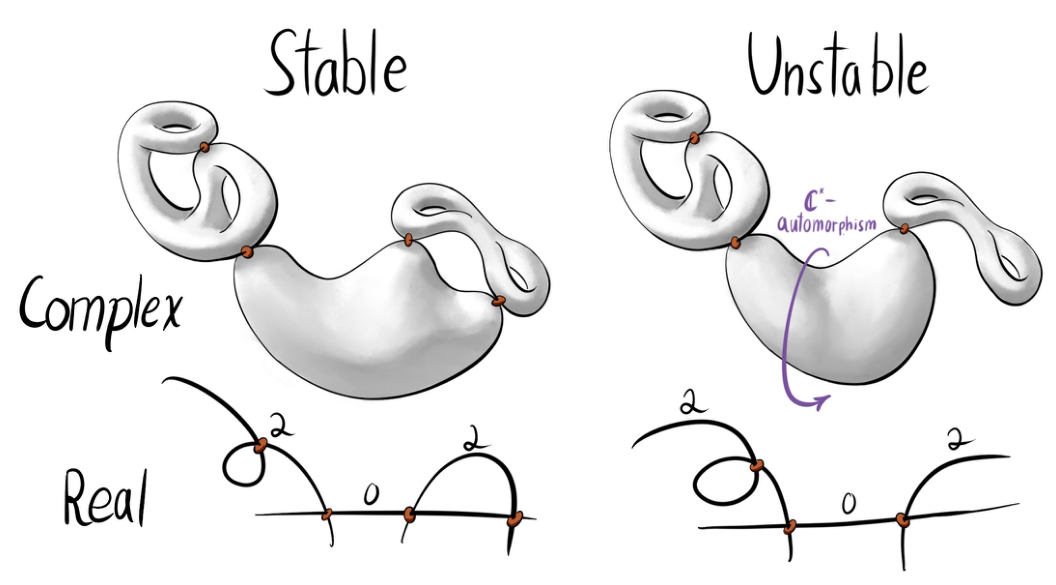
\includegraphics[width=.52\textwidth]{figures/stable-opening.png}};
\begin{scope}[x={(im.south east)},y={(im.north west)}]
\node[fill=white,inner sep=2pt] at (.32,.93) {稳定};
\node[fill=white,inner sep=2pt] at (.76,.93) {不稳定};
\node[fill=white,inner sep=2pt] at (.04,.53) {复};
\node[fill=white,inner sep=2pt] at (.06,.18) {实};
\node[fill=white,inner sep=1pt,font=\tiny,text=violet] at (.77,.69) {$\mathbb C^*$-自同构};
\end{scope}\end{tikzpicture}
\end{center}
% The source omits a caption but begins its numbered statements at 6.3.2.
\setcounter{theorem}{1}
\begin{definition}[稳定, 半稳定与预稳定曲线]\label{src:6.3.2}
代数闭域 $k$ 上亏格为 $g$ 的 $n$-点连通结点射影曲线 $(C,\allowbreak p_1,\allowbreak \ldots,\allowbreak p_n)$ 称为\textit{稳定}的, 若
\begin{enumerate}[(1)]
\item $p_1,\allowbreak \ldots,\allowbreak p_n\in C(k)$ 是互异光滑点,
\item $C$ 不是没有标记点的亏格 $1$ 曲线, 即 $(g,\allowbreak n)\neq(1,\allowbreak 0)$, 且
\item 每条光滑不可约有理子曲线 $\mathbb P^1\subseteq C$ 含有至少 $3$ 个特殊点.
\end{enumerate}
若 (1)--(2) 成立, 且将 (3) 换为每条光滑有理子曲线含有至少 $2$ 个 (而非 $3$ 个) 特殊点, 则称 $(C,\allowbreak p_i)$ 为\textit{半稳定}的. 若仅 (1)--(2) 成立, 则称 $(C,\allowbreak p_i)$ 为\newterm{预稳定}{prestable}的.
\end{definition}
有如下蕴含:
\[
\boxed{\text{稳定}\Rightarrow\text{半稳定}\Rightarrow\text{预稳定}\Rightarrow n\text{-点结点曲线}.}
\]
在无标记点的情形, 曲线是预稳定曲线当且仅当它是结点曲线. 当 $k$ 非代数闭时, 稳定性定义中的条件 (3) 需要调整; 见命题~\bookref{6.3.15}.
\begin{remark}\label{src:6.3.3}
注意若 $(g,\allowbreak n)\in\{(0,\allowbreak 0),\allowbreak (0,\allowbreak 1),\allowbreak (0,\allowbreak 2),\allowbreak (1,\allowbreak 0)\}$, 或等价地 $2g-2+n\leq0$, 则不存在亏格为 $g$ 的 $n$-点稳定曲线. 我们常加上 $2g-2+n>0$ 的条件以排除这些特殊情形.
\end{remark}
\begin{figure}[H]\centering\begin{minipage}[t]{.23\textwidth}\centering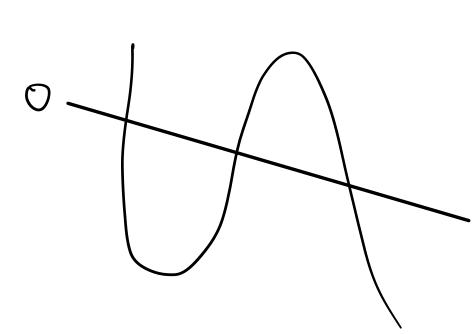
\includegraphics[width=.95\linewidth,height=1.7cm,keepaspectratio]{figures/stable-example-1.png}\\{\small\color{red} 稳定}\end{minipage}
\begin{minipage}[t]{.23\textwidth}\centering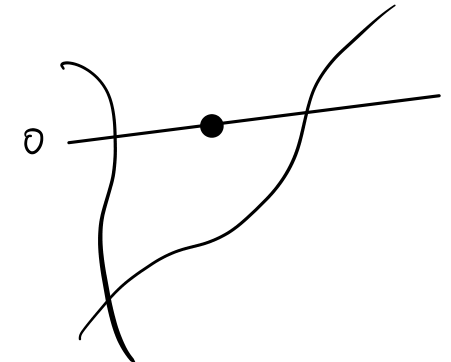
\includegraphics[width=.95\linewidth,height=1.7cm,keepaspectratio]{figures/stable-example-2.png}\\{\small\color{red} 稳定}\end{minipage}
\begin{minipage}[t]{.23\textwidth}\centering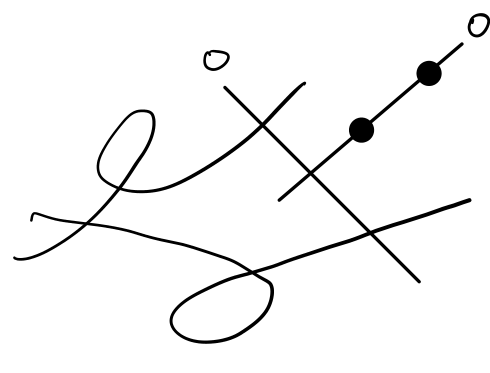
\includegraphics[width=.95\linewidth,height=1.7cm,keepaspectratio]{figures/stable-example-3.png}\\{\small\color{red} 稳定}\end{minipage}
\begin{minipage}[t]{.23\textwidth}\centering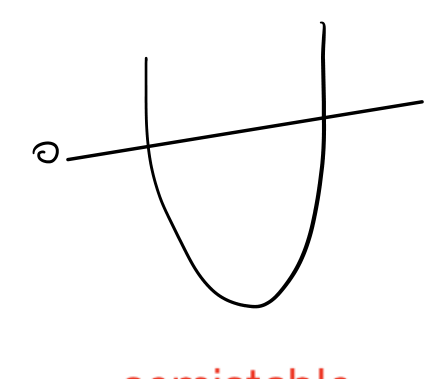
\includegraphics[width=.95\linewidth,height=1.7cm,keepaspectratio]{figures/stable-example-4.png}\\{\small\color{red} 半稳定\\不稳定}\end{minipage}
\medskip\par
\begin{minipage}[t]{.23\textwidth}\centering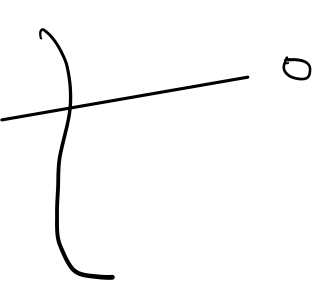
\includegraphics[width=.95\linewidth,height=1.7cm,keepaspectratio]{figures/stable-example-5.png}\\{\small\color{red} 预稳定\\不半稳定}\end{minipage}
\begin{minipage}[t]{.23\textwidth}\centering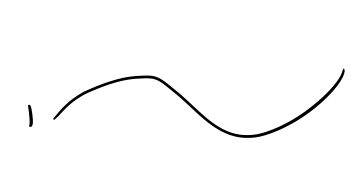
\includegraphics[width=.95\linewidth,height=1.7cm,keepaspectratio]{figures/stable-example-6.png}\\{\small\color{red} 非预稳定}\end{minipage}
\begin{minipage}[t]{.23\textwidth}\centering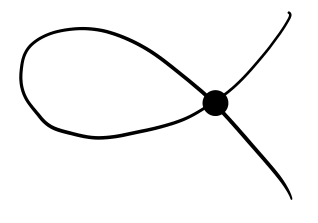
\includegraphics[width=.95\linewidth,height=1.7cm,keepaspectratio]{figures/stable-example-7.png}\\{\small\color{red} 非预稳定}\end{minipage}
\begin{minipage}[t]{.23\textwidth}\centering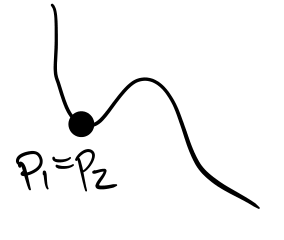
\includegraphics[width=.95\linewidth,height=1.7cm,keepaspectratio]{figures/stable-example-8.png}\\{\small\color{red} 非预稳定}\end{minipage}

\caption{稳定, 半稳定和预稳定曲线的例子.}\label{src:6.3.4}
\end{figure}
稳定曲线 $(C,\allowbreak p_1,\allowbreak \ldots,\allowbreak p_n)$ 的自同构是满足 $\alpha(p_i)=p_i$ 的自同构 $\alpha:C\xrightarrow{\sim}C$. 用 $\operatorname{Aut}(C,\allowbreak p_1,\allowbreak \ldots,\allowbreak p_n)$ 表示自同构的抽象群. 也回顾: 若 $C$ 是亏格 $g\geq2$ 的几何光滑, 连通射影曲线, 则 $\operatorname{Aut}(C)$ 有限 (命题~\bookref{6.1.8}).
\begin{proposition}\label{src:6.3.5}
设 $(C,\allowbreak p_1,\allowbreak \ldots,\allowbreak p_n)$ 是代数闭域 $k$ 上的 $n$-点预稳定曲线. 以下条件等价:
\begin{enumerate}[(1)]
\item $(C,\allowbreak p_1,\allowbreak \ldots,\allowbreak p_n)$ 稳定,
\item $\operatorname{Aut}(C,\allowbreak p_1,\allowbreak \ldots,\allowbreak p_n)$ 有限, 且
\item $\omega_C(p_1+\cdots+p_n)$ 丰沛.
\end{enumerate}
\end{proposition}
\begin{proof}
(1) $\Leftrightarrow$ (2) 由习题~\bookref{6.3.7} 及以下事实得到: 光滑预稳定 $n$-点曲线 $(C,\allowbreak p_i)$ 的自同构群具有正维数, 仅当 $C=\mathbb P^1$ 且 $n\leq2$, 或 $C$ 是亏格 $1$ 曲线且 $n=0$ (见命题~\bookref{6.1.8}). 为证明与 (3) 等价, 使用以下事实: 对子曲线 $T\subseteq C$, 有 $\omega_C|_T=\omega_T(T\cap T^c)$ (习题~\bookref{6.2.21}). 线丛 $\omega_C(p_1+\cdots+p_n)$ 丰沛当且仅当它在每个不可约分支 $T\subseteq C$ 上的限制
\begin{equation}\label{src:6.3.6}
\omega_C(p_1+\cdots+p_n)|_T=\omega_T\left(\sum_{p_i\in T}p_i+(T\cap T^c)\right)
\end{equation}
丰沛. 若 $T$ 的亏格 $g(T)$ 至少为 $2$, 则 $\omega_T$ 丰沛, 因而~\bookeqref{6.3.6} 也丰沛. 若 $g(T)=1$, 则~\bookeqref{6.3.6} 丰沛当且仅当 $n\geq1$ 或 $T$ 与补曲线 $T^c$ 相交. 若 $g(T)=0$, 则~\bookeqref{6.3.6} 丰沛当且仅当 $T$ 含有至少 $3$ 个特殊点.
\end{proof}
\begin{exercise}[带标记的正规化]\label{src:6.3.7}
设 $(C,\allowbreak p_1,\allowbreak \ldots,\allowbreak p_n)$ 是 $n$-点预稳定曲线. 设 $\pi:\widetilde C\to\allowbreak C$ 是正规化, $\widetilde p_i\in\widetilde C$ 是 $p_i$ 的唯一原像, $\widetilde q_1,\allowbreak \ldots,\allowbreak \widetilde q_m\in\widetilde C$ 是结点原像的一个排序. 称 $(\widetilde C,\allowbreak \widetilde p_i,\allowbreak \widetilde q_j)$ 为 $(C,\allowbreak p_i)$ 的\newterm{带标记的正规化}{pointed normalization}. 证明 $(C,\allowbreak p_i)$ 稳定当且仅当 $(\widetilde C,\allowbreak \widetilde p_i,\allowbreak \widetilde q_j)$ 的每个带标记连通分支 (即 $\widetilde C$ 的每个连通分支连同落在其上的 $\widetilde p_i,\allowbreak \widetilde q_j$) 稳定.
\end{exercise}
\begin{exercise}\label{src:6.3.8}
设 $(C,\allowbreak p_1,\allowbreak \ldots,\allowbreak p_n)$ 是 $n$-点预稳定曲线.
\begin{enumerate}[(a)]
\item 证明自同构群概形 $\underline{\operatorname{Aut}}(C,\allowbreak p_i)$ 是代数群.
\item 证明 $\underline{\operatorname{Aut}}(C,\allowbreak p_i)$ 自然是带标记正规化 $(\widetilde C,\allowbreak \widetilde p_i,\allowbreak \widetilde q_j)$ 的自同构群 $\underline{\operatorname{Aut}}(\widetilde C,\allowbreak \widetilde p_i,\allowbreak \widetilde q_j)$ 的闭子群.
\item 证明 $\underline{\operatorname{Aut}}(C,\allowbreak p_i)^0=\underline{\operatorname{Aut}}(\widetilde C,\allowbreak \widetilde p_i,\allowbreak \widetilde q_j)^0$, 但一般有 $\underline{\operatorname{Aut}}(C,\allowbreak p_i)\neq\underline{\operatorname{Aut}}(\widetilde C,\allowbreak \widetilde p_i,\allowbreak \widetilde q_j)$.
\end{enumerate}
\end{exercise}
\paragraph{对偶图.}
\textit{顶点带权的 $n$-标记图} $\Gamma=(G,\allowbreak w,\allowbreak m)$ 是以下数据: 具有顶点集 $V(G)$ 和边集 $E(G)$ 的有限, 连通无向图 $G$ (允许环和重边), 权函数 $w:V(G)\to\mathbb Z_{\geq0}$, 以及 $n$-标记 $m:\{1,\allowbreak \ldots,\allowbreak n\}\to\allowbreak V(G)$. 每个顶点 $m(i)\in V(G)$ 视为一条半边. $\Gamma$ 的亏格是
\[
g(\Gamma)=g(G)+\sum_{v\in V(G)}w(v),
\]
其中 $g(G)=|E(G)|-|V(G)|+1$ 表示 $G$ 的亏格, 即将 $G$ 视为一维 CW 复形时的第一 Betti 数. 若对每个顶点 $v\in V(G)$,
\[
2w(v)-2+\operatorname{val}(v)+|m^{-1}(v)|>0,
\]
则称顶点带权的 $n$-标记图 $\Gamma$ \textit{稳定}. 这里 $\operatorname{val}(v)$ 是 $v$ 的度, 定义为包含 $v$ 的边数, 环计两次. 换言之, 稳定性指对每个顶点 $v$, 以下之一成立: (a) $w(v)\geq2$, (b) $w(v)=1$ 且 $v$ 属于一条边或半边, 或 (c) $w(v)=0$ 且 $\operatorname{val}(v)+|m^{-1}(v)|\geq3$.
\begin{figure}[H]\centering\begin{tikzcd}[column sep=large]
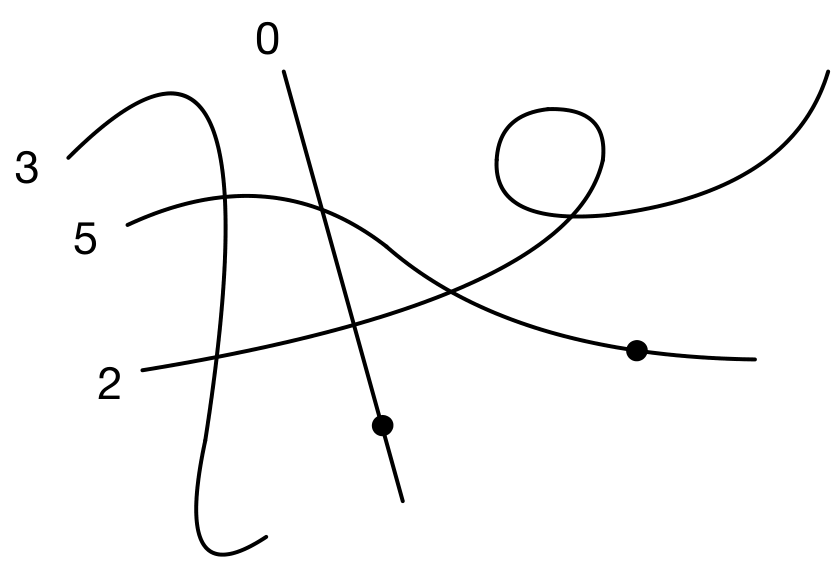
\includegraphics[width=.34\textwidth]{figures/stable-dual-curve.png}\arrow[r,"\text{对偶图}",rightsquigarrow]&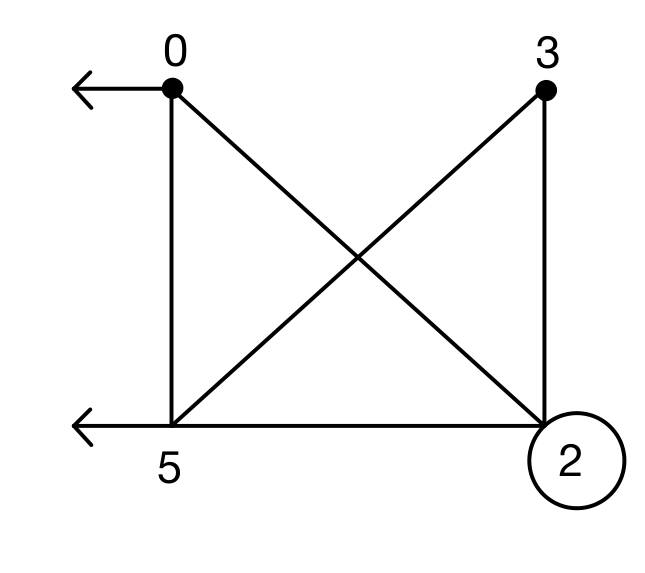
\includegraphics[width=.28\textwidth]{figures/stable-dual-graph.png}
\end{tikzcd}

\begingroup\renewcommand{\thefigure}{6.3.8}\renewcommand{\theHfigure}{6.3.8-figure}\caption{亏格为 $13$ 的曲线及其对偶图.}\label{src:6.3.8-figure}\endgroup
\addtocounter{theorem}{-1}
\end{figure}
\begin{definition}[对偶图]\label{src:6.3.9}
$n$-点预稳定曲线 $(C,\allowbreak p_1,\allowbreak \ldots,\allowbreak p_n)$ 的\newterm{对偶图}{dual graph} 定义为 $\Gamma=(G,\allowbreak w,\allowbreak m)$, 其中 $G$ 的顶点 $v_i$ 对应于 $C$ 的不可约分支 $C_i$, 权 $w(v_i)$ 是 $C_i$ 的几何亏格. 对落在分支 $C_i,\allowbreak C_j$ 上的每个结点 $q$, 有连接 $v_i,\allowbreak v_j$ 的边 $e_q$, 标记 $m(i)$ 是满足 $p_i\in C_j$ 的顶点 $v_j$.
\end{definition}
\begin{exercise}[容易]\label{src:6.3.10}
证明 $n$-点预稳定曲线 $(C,\allowbreak p_i)$ 稳定当且仅当其对偶图 $\Gamma$ 稳定, 且 $C$ 的亏格等于 $\Gamma$ 的亏格.
\end{exercise}
稳定曲线的叠 $\overline{\mathcal M}_{g,\allowbreak n}$ 按对偶图具有一个分层 (习题~\bookref{6.6.23}).
\begin{figure}[H]\centering\begin{tikzcd}[column sep=large,row sep=small]
&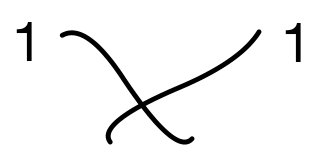
\includegraphics[width=.13\textwidth,height=1cm,keepaspectratio]{figures/stable-g2-curve-2.png}\arrow[r]&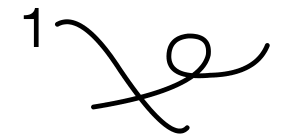
\includegraphics[width=.13\textwidth,height=1cm,keepaspectratio]{figures/stable-g2-curve-3.png}\arrow[r]&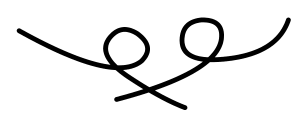
\includegraphics[width=.13\textwidth,height=1cm,keepaspectratio]{figures/stable-g2-curve-4.png}\\
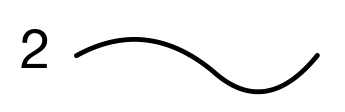
\includegraphics[width=.13\textwidth,height=1cm,keepaspectratio]{figures/stable-g2-curve-1.png}\arrow[ur]\arrow[dr]&&&\\
&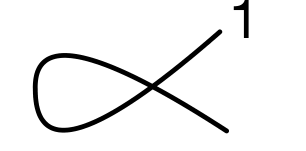
\includegraphics[width=.13\textwidth,height=1cm,keepaspectratio]{figures/stable-g2-curve-5.png}\arrow[r]\arrow[uur]&
\includegraphics[width=.13\textwidth,height=1cm,keepaspectratio]{figures/stable-g2-curve-6.png}\arrow[r]\arrow[uur]&
\includegraphics[width=.13\textwidth,height=1cm,keepaspectratio]{figures/stable-g2-curve-7.png}
\end{tikzcd}
\par\smallskip\noindent\rule{.85\textwidth}{.4pt}\par\smallskip
\begin{tikzcd}[column sep=large,row sep=small]
&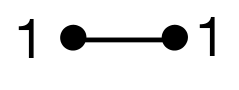
\includegraphics[width=.13\textwidth,height=1cm,keepaspectratio]{figures/stable-g2-graph-2.png}\arrow[r]&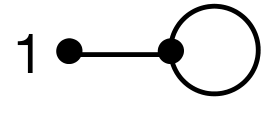
\includegraphics[width=.13\textwidth,height=1cm,keepaspectratio]{figures/stable-g2-graph-3.png}\arrow[r]&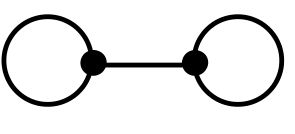
\includegraphics[width=.13\textwidth,height=1cm,keepaspectratio]{figures/stable-g2-graph-4.png}\\

\includegraphics[width=.13\textwidth,height=1cm,keepaspectratio]{figures/stable-g2-graph-1.png}\arrow[ur]\arrow[dr]&&&\\
&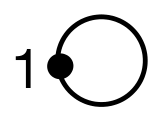
\includegraphics[width=.13\textwidth,height=1cm,keepaspectratio]{figures/stable-g2-graph-5.png}\arrow[r]\arrow[uur]&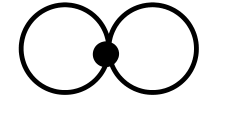
\includegraphics[width=.13\textwidth,height=1cm,keepaspectratio]{figures/stable-g2-graph-6.png}\arrow[r]\arrow[uur]&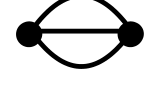
\includegraphics[width=.13\textwidth,height=1cm,keepaspectratio]{figures/stable-g2-graph-7.png}
\end{tikzcd}

\begingroup\renewcommand{\thefigure}{6.3.10}\renewcommand{\theHfigure}{6.3.10-figure}\caption{无标记点的亏格 $2$ 顶点带权图共有七种. 上方显示曲线, 下方显示其对偶图. 箭头表示特殊化. 从左列向右列, $\overline{\mathcal M}_2$ 中参数化具有给定对偶图的曲线的子叠的维数依次为 $3$, $2$, $1$, $0$.}\label{src:6.3.10-figure}\endgroup
\addtocounter{theorem}{-1}
\end{figure}
\begin{exercise}\label{src:6.3.11}
\begin{enumerate}[(a)]
\item 分类亏格为 $1$ 的稳定顶点带权 $2$-标记图.
\item 确定亏格为 $3$ 的稳定顶点带权 $0$-标记图的同构类数.
\end{enumerate}
\end{exercise}
\subsection{有理尾与有理桥}\label{src:6.3.2-subsection}
\begin{definition}[有理尾与有理桥]\label{src:6.3.12}
设 $(C,\allowbreak p_1,\allowbreak \ldots,\allowbreak p_n)$ 是域 $k$ 上的 $n$-点预稳定曲线. 对亏格为 $0$, 且补曲线 $E^c=\overline{C\setminus E}$ 非空的不可约光滑子曲线 $E\subseteq C$, 我们称其为
\begin{itemize}
\item \newterm{有理尾}{rational tail}, 若概形意义的交 $E\cap E^c$ 是单个约化点 $x$, $\mathrm H^0(E,\allowbreak \mathcal O_E)\cong\kappa(x)$, 且 $E$ 不含标记点; 以及
\item \newterm{有理桥}{rational bridge}, 若概形意义的交 $E\cap E^c$ 在 $\mathrm H^0(E,\allowbreak \mathcal O_E)$ 上的次数为 $2$, 且 $E$ 不含标记点; 或者 $E$ 只含一个标记点 $p_j$, 且 $E$ 是 $(C,\allowbreak p_1,\allowbreak \ldots,\allowbreak \widehat p_j,\allowbreak \ldots,\allowbreak p_n)$ 的有理尾.
\end{itemize}
\end{definition}
在代数闭域上, 每条不可约光滑有理子曲线 $E$ 同构于 $\mathbb P^1$. $E$ 是有理尾当且仅当 $E\cdot E^c=1$ 且 $E$ 没有标记点; $E$ 是有理桥当且仅当 $E\cdot E^c=2$ 且 $E$ 没有标记点, 或 $E\cdot E^c=1$ 且 $E$ 恰有一个标记点.
\begin{figure}[H]\centering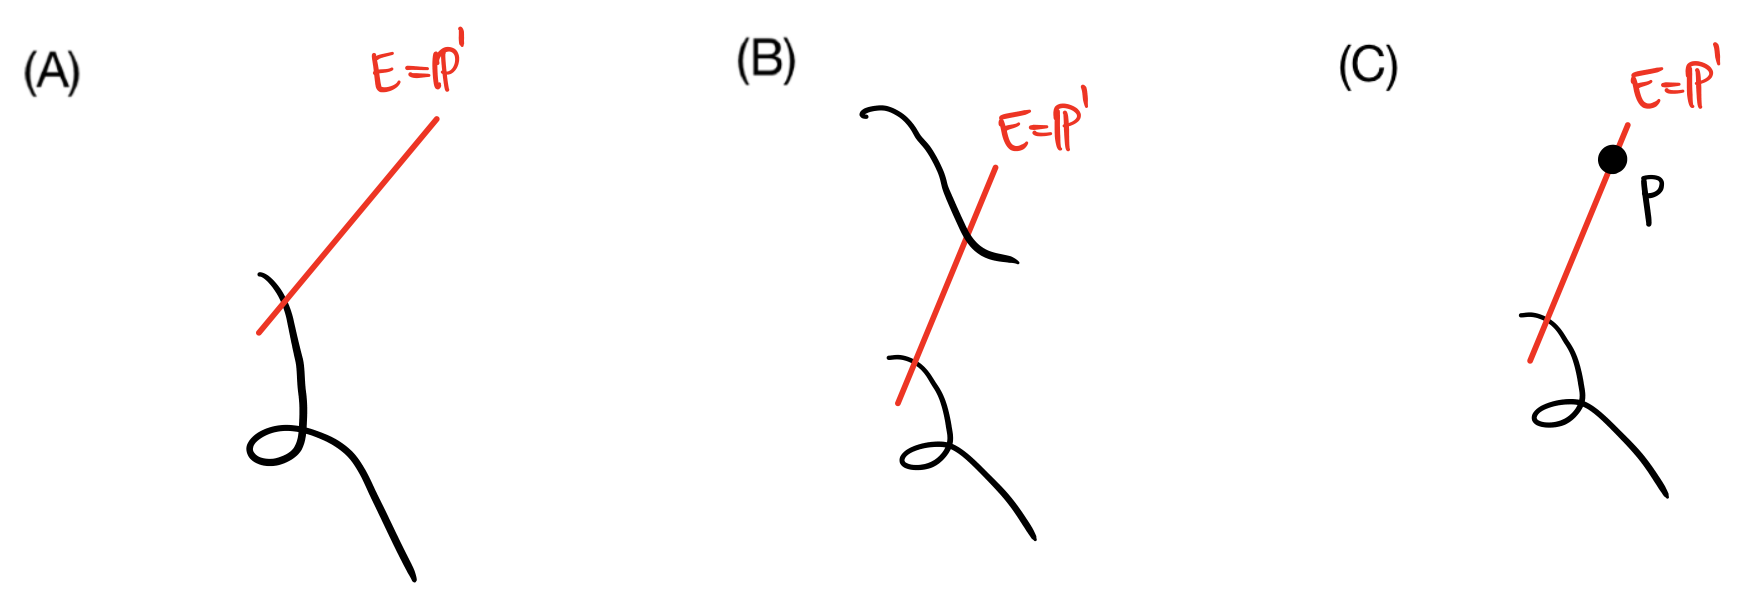
\includegraphics[width=.64\textwidth]{figures/fig-6.3.12.png}
\begingroup\renewcommand{\thefigure}{6.3.12}\renewcommand{\theHfigure}{6.3.12-figure}\caption{(A) 含有一个有理尾, (B) 与 (C) 含有有理桥.}\label{src:6.3.12-figure}\endgroup\addtocounter{theorem}{-1}
\end{figure}
在任意域上, 有理尾和有理桥的分类更为微妙. 考虑到有理曲线的分类也更复杂 (见习题~\bookref{6.1.13} 和~\bookref{6.1.14}), 这并不意外.
\begin{lemma}\label{src:6.3.13}
设 $(C,\allowbreak p_i)$ 是域 $k$ 上的 $n$-点预稳定曲线.
\begin{enumerate}[(1)]
\item 若 $E$ 是有理尾, $k':=\mathrm H^0(E,\allowbreak \mathcal O_E)=\kappa(x)$, 则 $k'$ 是 $k$ 的有限可分域扩张, 且 $E\cong\mathbb P_{k'}^1$.
\item 若 $E$ 是没有标记点的有理桥, 则 $k':=\mathrm H^0(E,\allowbreak \mathcal O_E)$ 是 $k$ 的有限可分域扩张, $k'':=\mathrm H^0(E\cap E^c,\allowbreak \mathcal O_{E\cap E^c})$ 是 $k'$ 的次数为 $2$ 的可分域扩张或 $k''=k'\times k'$.
\end{enumerate}
\end{lemma}
\begin{proof}
两种情形下, 由于 $E$ 约化且连通, $k'=\mathrm H^0(E,\allowbreak \mathcal O_E)$ 是域. 对 (1), 交点 $x=E\cap E^c$ 是结点, 因而 $k'=\kappa(x)$ 是 $k$ 的可分域扩张 (命题~\bookref{6.2.4}). 通过结构映射 $E\to\Spec\Gamma(E,\allowbreak \mathcal O_E)=\Spec k'$ 将 $E$ 视为 $k'$ 上的概形, 由其不可约, 光滑, 亏格为 $0$ 且含有有理点, 得到 $E\cong\mathbb P_{k'}^1$. 对 (2), $E\cap E^c$ 的点是 $C$ 中的结点, 但在 $E,\allowbreak E^c$ 中都是光滑点. 由 $\dim_{k'}k''=2$, 或 $k''$ 是域, 此时由命题~\bookref{6.2.4} 它在 $k$ 上可分; 或 $k''=k'\times k'$.
\end{proof}
\begin{exercise}\label{src:6.3.14}
若 $K/k$ 是域扩张, 则 $(C,\allowbreak p_i)$ 有有理尾 (分别地, 有理桥) 当且仅当 $(C\times_k K,\allowbreak p_i\times_k K)$ 有有理尾 (分别地, 有理桥).
\end{exercise}
稳定性等价于不含有理尾或有理桥.
\begin{proposition}\label{src:6.3.15}
设 $(C,\allowbreak p_i)$ 是域 $k$ 上亏格为 $g$ 的 $n$-点预稳定曲线. 若 $K$ 是包含 $k$ 的代数闭域, 则 $(C\times_k K,\allowbreak p_i\times_k K)$ 稳定 (分别地, 半稳定) 当且仅当 $(C,\allowbreak p_i)$ 不含有理尾或有理桥 (分别地, 不含有理尾).
\end{proposition}
\begin{proof}
在代数闭域上, 稳定 (分别地, 半稳定) 等价于不含有理尾或有理桥 (分别地, 有理尾). 因此结论由有理尾或有理桥的存在性不受域扩张影响这一事实 (习题~\bookref{6.3.14}) 得到.
\end{proof}
\begin{remark}[与 $-1$ 和 $-2$ 曲线的关系]\label{src:6.3.16}
设 $C\to\Delta=\Spec R$ 是 DVR $R$ 上的结点曲线族, 剩余域 $k$ 代数闭, 一般纤维光滑. 若 $E\cong\mathbb P^1\subseteq C_0$ 是中心纤维中的光滑有理子曲线, 则 $E^2=-E\cdot E^c$ (由恒等式 $0=E\cdot C_0=E\cdot E+E\cdot E^c$ 得到). 因而若 $E$ 是有理尾 (分别地, 无标记点的有理桥), 则 $E^2=-1$ (分别地, $E^2=-2$).
\end{remark}
\begin{figure}[H]\centering\begin{tikzcd}[column sep=large,row sep=small]
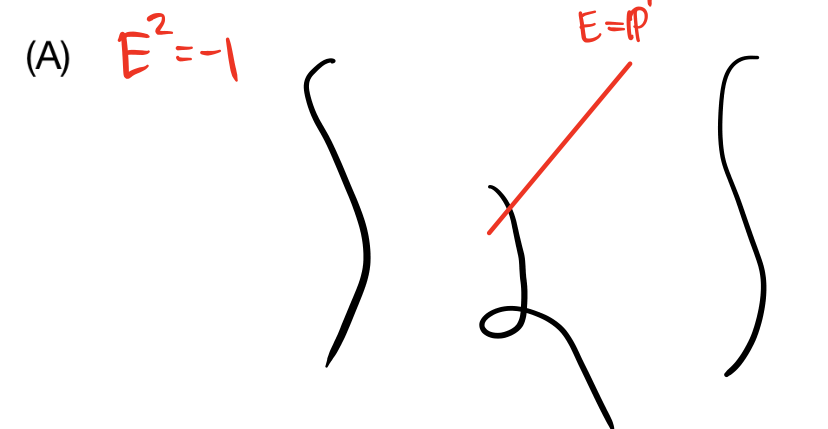
\includegraphics[width=.32\textwidth]{figures/stable-contract-tail-top.png}\arrow[d]&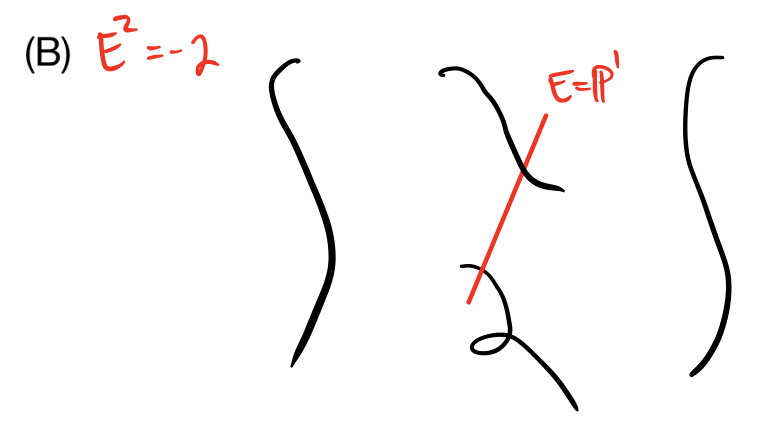
\includegraphics[width=.32\textwidth]{figures/stable-contract-bridge-top.png}\arrow[d]\\
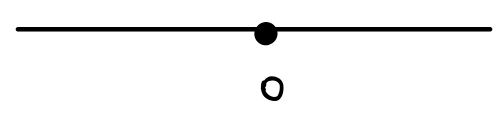
\includegraphics[width=.2\textwidth]{figures/stable-contract-tail-bottom.png}&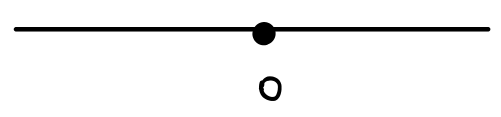
\includegraphics[width=.2\textwidth]{figures/stable-contract-bridge-bottom.png}
\end{tikzcd}

\begingroup\renewcommand{\thefigure}{6.3.16}\renewcommand{\theHfigure}{6.3.16-figure}\caption{在 (A) (分别地, (B)) 中, 例外分支 $E$ 与曲线其余部分在一个点 (分别地, 两个点) 相交, 且 $E^2=-1$ (分别地, $E^2=-2$).}\label{src:6.3.16-figure}\endgroup\addtocounter{theorem}{-1}
\end{figure}
后文预稳定曲线族的稳定收缩 (\bookref{6.6.6}) 将推广以下习题.
\begin{exercise}[困难]\label{src:6.3.17}
设 $C\to\Delta=\Spec R$ 是 DVR $R$ 上的结点曲线族, 一般纤维光滑. 对中心纤维中的任意有理尾或有理桥 $E\subset C_0$, 证明存在 $E$ 的收缩 $C\to\allowbreak C'$, 其中 $C'\to\Delta$ 是结点曲线族.

\textit{提示:} Castelnuovo 收缩定理 (\bookref{B.2.6}) 给出收缩 $C\to\allowbreak C'$ 的存在性. 难点在于说明中心纤维 $C'_0$ 是结点曲线. 可使用极小模型纲领中的事实: $C'_0$ 是结点曲线当且仅当对 $(C',\allowbreak C'_0)$ 是对数典范的~\cite[推论 2.32, 定理 4.9(2)]{Kol13}, 并利用 $(C,\allowbreak C_0)$ (分别地, $(C,\allowbreak C_0-E)$) 是对数典范的, 说明后一性质成立.
\end{exercise}
\subsection{对偶化层的正性}\label{src:6.3.3-subsection}
\begin{exercise}[中等]\label{src:6.3.18}
设 $(C,\allowbreak p_1,\allowbreak \ldots,\allowbreak p_n)$ 是代数闭域 $k$ 上的 $n$-点预稳定曲线, $L:=\omega_C(p_1+\cdots+p_n)$.
\begin{enumerate}[(a)]
\item 若 $(C,\allowbreak p_i)$ 稳定, 证明 $k\geq3$ 时 $L^{\otimes k}$ 甚丰沛, 且 $k\geq2$ 时 $\mathrm H^1(C,\allowbreak (\omega_C(p_1+\cdots+p_n))^{\otimes k})=0$.
\item 对 $k\geq2$, 证明 $(C,\allowbreak p_i)$ 半稳定当且仅当 $L^{\otimes k}$ 无基点.
\end{enumerate}
\textit{提示:} 对 (a), 证明 $L^{\otimes k}$ 的整体截面分离点和切向量, 换言之, 映射
\[
\begin{aligned}
\mathrm H^0(C,L^{\otimes k})&\to(L^{\otimes k}\otimes\kappa(x))\oplus(L^{\otimes k}\otimes\kappa(y)),\\
\mathrm H^0(C,L^{\otimes k})&\to L^{\otimes k}\otimes\mathcal O_{C,x}/\mathfrak m_x^2
\end{aligned}
\]
满射. 利用 Serre 对偶, 并按 $x,\allowbreak y$ 为光滑点或结点分类讨论. 另见~\cite[定理 2]{DM69}, \cite[引理 10.6.1]{ACG11}, \cite[Tag 0E8X]{SP} 和~\cite[命题 13.2.17]{Ols16}.
\end{exercise}
\begin{exercise}[很好的练习]\label{src:6.3.19}
若 $C$ 是亏格分别为 $i$ 和 $g-i$ 的曲线沿单个结点 $p=C_1\cap C_2$ 的结点并 $C_1\cup C_2$, 证明 $\omega_C$ 在 $p$ 处有基点.
\end{exercise}
\subsection{稳定曲线族}\label{src:6.3.4-subsection}
\begin{definition}\label{src:6.3.20}
概形 $S$ 上的\textit{$n$-点曲线族} 是代数空间的固有, 平坦有限表现态射 $C\to\allowbreak S$, 配备 $n$ 个截面 $\sigma_1,\allowbreak \ldots,\allowbreak \sigma_n:S\to\allowbreak C$, 使得每个几何纤维 $C_s$ 都是 $\Spec\kappa(s)$ 上的曲线 (例如一维有限型 $\kappa(s)$-概形).

\textit{$n$-点稳定曲线族} (分别地, \textit{半稳定曲线族}, \textit{预稳定曲线族}, \textit{结点曲线族}) 是每个几何纤维 $(C_s,\allowbreak \sigma_1(s),\allowbreak \ldots,\allowbreak \sigma_n(s))$ 都稳定 (分别地, 半稳定, 预稳定, 结点) 的 $n$-点曲线族.
\end{definition}
\begin{remark}[注意]\label{src:6.3.21}
若 $(C\to\allowbreak S,\allowbreak \sigma_i)$ 是概形 $S$ 上的稳定曲线族, 则 $C\to\allowbreak S$ 必为射影态射 (命题~\bookref{6.3.22}), 因而 $C$ 是概形. 虽然域上每个一维分离有限型代数空间都是概形 (定理~\bookref{5.5.32}), 在相对情形中, 族的总空间 $C$ 却未必是概形. 存在亏格 $0$ 的预稳定曲线族~\cite[例 2.3]{Ful10} 和亏格 $1$ 的光滑曲线族~\cite[XIII.3.2]{Ray70}, 其总空间不是概形; 另见例~\bookref{3.1.16}. 下一节将证明所有曲线 (分别地, 结点曲线, 半稳定曲线, 预稳定曲线) 的叠是代数叠, 特别地满足曲线族的下降条件; 该结果要求允许族的总空间为代数空间.
\end{remark}
对 $n$-点曲线族 (分别地, 结点曲线族), 不要求标记点互异或落在 $C\to\allowbreak S$ 的相对光滑轨迹上. 对稳定, 半稳定和预稳定曲线族, 标记点互异且避开结点. 若 $(C\to\allowbreak S,\allowbreak \sigma_i)$ 是 $n$-点预稳定曲线族, 则 $C\to\allowbreak S$ 是局部完全交态射. 因而有相对对偶化线丛 $\omega_{C/S}$, 与基变换 $T\to\allowbreak S$ 相容, 特别地, 在 $C\to\allowbreak S$ 的每个纤维上限制为对偶化线丛 $\omega_{C_s}$; 见~\cite{Har66c} 或~\cite[\S 6.4]{Liu02}. 每个截面 $\sigma_i$ 的像是包含在光滑轨迹中的除子, 可形成线丛 $\omega_{C/S}(\sigma_1+\cdots+\sigma_n)$.

以下陈述将命题~\bookref{6.3.5} 推广到曲线族. 用 $\underline{\operatorname{Aut}}(C/S,\allowbreak \sigma_1,\allowbreak \ldots,\allowbreak \sigma_n)$ 表示参数化 $n$-点预稳定曲线族的自同构的 $S$ 上局部有限型群概形.
\begin{proposition}\label{src:6.3.22}
设 $(C\to\allowbreak S,\allowbreak \sigma_i)$ 是概形 $S$ 上亏格为 $g$ 的 $n$-点预稳定曲线族. 以下条件等价:
\begin{enumerate}[(1)]
\item $(C\to\allowbreak S,\allowbreak \sigma_i)$ 是稳定曲线族,
\item $\underline{\operatorname{Aut}}(C/S,\allowbreak \sigma_1,\allowbreak \ldots,\allowbreak \sigma_n)\to\allowbreak S$ 拟有限, 且
\item $\omega_{C/S}(\sigma_1+\cdots+\sigma_n)$ 在 $S$ 上相对丰沛.
\end{enumerate}
特别地, $n$-点稳定曲线族是概形的射影态射.
\end{proposition}
\begin{proof}
每个条件均可在几何纤维上检验, 因而结论由命题~\bookref{6.3.5} 得到.
\end{proof}
$\overline{\mathcal M}_{g,\allowbreak n}$ 的分离性 (命题~\bookref{6.5.20}) 说明 $\underline{\operatorname{Aut}}(C/S,\allowbreak \sigma_1,\allowbreak \ldots,\allowbreak \sigma_n)\to\allowbreak S$ 事实上是有限群概形.

以下是光滑曲线族的性质 (\bookref{6.1.16}) 的推广, 其证明相同, 只需使用代数闭域上的稳定 $n$-点曲线 $(C,\allowbreak p_i)$ 的 $\omega_C(p_1+\cdots+p_n)^{\otimes3}$ 的甚丰沛性 (习题~\bookref{6.3.18}).
\begin{proposition}[稳定曲线族的性质]\label{src:6.3.23}
设 $(C\to\allowbreak S,\allowbreak \sigma_i)$ 是亏格为 $g$ 的 $n$-点稳定曲线族, $L:=\omega_{C/S}(\sum_i\sigma_i)$. 若 $k\geq3$, 则 $L^{\otimes k}$ 相对甚丰沛, 且 $\pi_*(L^{\otimes k})$ 是秩为 $(2k-1)(g-1)+kn$ 的向量丛.\hfill$\square$
\end{proposition}
\begin{proposition}[稳定性的开放性]\label{src:6.3.24}
设 $(\pi:C\to\allowbreak S,\allowbreak \sigma_i)$ 是 $n$-点曲线族. 使 $(C_s,\allowbreak \sigma_i(s))$ 稳定 (分别地, 半稳定, 预稳定, 结点) 的点 $s\in S$ 的轨迹是开集.
\end{proposition}
\begin{proof}
先断言结点轨迹是开集. 当 $C$ 是概形时, 由结点的局部结构 (\bookref{6.2.26}), 在其纤维中为光滑点或结点的点的轨迹 $C^{\leq\mathrm{nod}}\subseteq C$ 是开集. 因而使 $C_s$ 具有比结点更坏的奇点的点 $s\in S$ 的轨迹, 等同于闭轨迹 $\pi(C\setminus C^{\leq\mathrm{nod}})\subseteq S$. 一般地, 可选取由概形给出的平展覆盖 $C'\to\allowbreak C$, 并利用 $p\in C$ 在纤维 $C_{\pi(p)}$ 中为结点当且仅当其原像 $p'\in C'$ 在纤维 $C'_{\pi(p)}$ 中为结点. 也可用命题~\bookref{6.2.24} 的刻画: $p\in C_s$ 为结点当且仅当 $C\to\allowbreak S$ 在 $p$ 处 syntomic 且 $\operatorname{Sing}(C/S)\to\allowbreak S$ 在 $p$ 处非分歧, 再利用 syntomic 轨迹和非分歧轨迹的开放性.

使 $\sigma_1(s),\allowbreak \ldots,\allowbreak \sigma_n(s)$ 是 $C_s$ 中互异光滑点的 $S$ 中轨迹是开集, 因而 $C_s$ 预稳定是开条件. 对 $n$-点预稳定曲线族 $(\pi:C\to\allowbreak S,\allowbreak \sigma_i)$, 使 $C_s$ 半稳定的点 $s\in S$ 的轨迹等同于 $\pi^*\pi_*L\to\allowbreak L$ 满射的开轨迹, 其中 $L:=\omega_{C/S}(\sum_i\sigma_i)$ (见习题~\bookref{6.3.25}).

最后给出两个论证, 说明在 $n$-点预稳定 (例如半稳定) 曲线族中, 稳定性是开条件. 首先, $\underline{\operatorname{Aut}}(C/S,\allowbreak \sigma_1,\allowbreak \ldots,\allowbreak \sigma_n)\to\allowbreak S$ 的纤维维数上半连续 (\bookref{B.1.9}), 因而使 $\operatorname{Aut}(C_s,\allowbreak \sigma_1(s),\allowbreak \ldots,\allowbreak \sigma_n(s))$ 有限的点 $s\in S$ 的轨迹是开集. 该条件刻画稳定性 (命题~\bookref{6.3.5}(2)), 所以这个开集就是稳定轨迹. 其次, 由丰沛性的开放性 (命题~\bookref{5.6.17}), 使 $\omega_{C/S}(\sum_i\sigma_i)|_{C_s}\cong\omega_{C_s}(\sum_i\sigma_i(s))$ 丰沛的点 $s\in S$ 的轨迹是开集, 而这也刻画稳定性 (命题~\bookref{6.3.5}(3)).
\end{proof}
\begin{exercise}\label{src:6.3.25}
设 $(\pi:C\to\allowbreak S,\allowbreak \sigma_i)$ 是 $n$-点预稳定曲线族, $L=\omega_{C/S}(\sigma_1+\cdots+\sigma_n)$. 对 $k\geq2$, 证明 $(C\to\allowbreak S,\allowbreak \sigma_i)$ 半稳定当且仅当 $\pi^*\pi_*L\to\allowbreak L$ 满射. 另见~\cite[Tag 0E6Y]{SP}.
\end{exercise}
\subsection{稳定曲线的形变理论}\label{src:6.3.5-subsection}
若 $C$ 是域 $k$ 上的光滑曲线, 则每个一阶形变局部平凡 (命题~\bookref{C.1.8}), 一阶形变的同构类集合 $\operatorname{Def}(C)$ 自然与 $\mathrm H^1(C,\allowbreak T_C)$ 双射 (命题~\bookref{C.1.11}). 更一般地, 高阶形变的自同构, 形变和障碍分别由 $i=0,\allowbreak 1,\allowbreak 2$ 时的 $\mathrm H^i(C,\allowbreak T_C)$ 分类 (命题~\bookref{C.2.4}). 另一方面, 结点奇点具有并非局部平凡的一阶形变, 例如 $\Spec k[x,\allowbreak y,\allowbreak \epsilon]/(xy-\epsilon)\to\Spec k[\epsilon]$.
\begin{proposition}\label{src:6.3.26}
设 $A'\twoheadrightarrow A$ 是剩余域为 $k$ 的 Artin 局部环的满射. 假设 $J=\ker(A'\to\allowbreak A)$ 满足 $\mathfrak m_{A'}J=0$. 设 $(\mathcal C\to\Spec A,\allowbreak \sigma_i)$ 是 $A$ 上的预稳定曲线族, $(C,\allowbreak p_i)$ 是其在剩余域 $k$ 上的基变换.
\begin{enumerate}[(1)]
\item $(\mathcal C\to\Spec A,\allowbreak \sigma_i)$ 在 $A'$ 上的一个形变的自同构群是 $\operatorname{Ext}^0_{\mathcal O_C}(\Omega_C(\sum_i p_i),\allowbreak \mathcal O_C\otimes_k J)$.
\item 将 $(\mathcal C\to\Spec A,\allowbreak \sigma_i)$ 形变到 $A'$ 上没有障碍.
\item $(\mathcal C\to\Spec A,\allowbreak \sigma_i)$ 在 $A'$ 上的形变的同构类集合是 $\operatorname{Ext}^1_{\mathcal O_C}(\Omega_C(\sum_i p_i),\allowbreak \mathcal O_C\otimes_k J)$ 下的 torsor, 且
\[
\begin{aligned}
&\dim_k\operatorname{Ext}^1_{\mathcal O_C}(\Omega_C(\sum_i p_i),\mathcal O_C)\\
&\qquad-\dim_k\operatorname{Ext}^0_{\mathcal O_C}(\Omega_C(\sum_i p_i),\mathcal O_C)=3g-3+n.
\end{aligned}
\]
\end{enumerate}
此外, 若 $(C,\allowbreak p_i)$ 稳定, 则 $\operatorname{Ext}^0_{\mathcal O_C}(\Omega_C(\sum_i p_i),\allowbreak \mathcal O_C)=0$, 即形变没有非平凡自同构, 且 $\dim_k\operatorname{Ext}^1_{\mathcal O_C}(\Omega_C(\sum_i p_i),\allowbreak \mathcal O_C)=3g-3+n$.
\end{proposition}
\begin{proof}
由于 $C$ 一般光滑且为局部完全交, 标记点 $p_i\in C$ 光滑, 命题~\bookref{C.2.4} (无标记点情形) 和命题~\bookref{C.2.8} (有标记点情形) 说明结点曲线 $C$ 的自同构, 形变和障碍由 $i=0,\allowbreak 1,\allowbreak 2$ 时的 $\operatorname{Ext}^i_{\mathcal O_C}(\Omega_C,\allowbreak I)$ 分类, 其中 $I\subseteq\mathcal O_C$ 是 $\{p_1,\allowbreak \ldots,\allowbreak p_n\}\subseteq C$ 的理想层. 由于 $I$ 定义 Cartier 除子, $I=\mathcal O_C(-\sum_i p_i)$, 因而自同构, 形变和障碍由 $\operatorname{Ext}^i_{\mathcal O_C}(\Omega_C(\sum_i p_i),\allowbreak \mathcal O_C)$ 分类.

为计算这些 Ext 群的维数, 先处理无标记点的情形. 因为 $\operatorname{Hom}_{\mathcal O_C}(\Omega_C,\allowbreak -)$ 是左正合函子的复合 $\Gamma\circ\mathcal H om_{\mathcal O_C}(\Omega_C,\allowbreak -)$, 有 Grothendieck 谱序列
\[
E_2^{p,q}=\mathrm H^p(C,\mathcal E xt^q_{\mathcal O_C}(\Omega_C,\mathcal O_C))\Rightarrow\operatorname{Ext}^{p+q}_{\mathcal O_C}(\Omega_C,\mathcal O_C),
\]
参见~\cite[定理 5.8.3]{Wei94}. 由于 $\dim C=1$, 当 $p\geq2$ 时 $E_2^{p,\allowbreak q}=0$. 因而 $E_2$ 页可画为:
\[
\begin{tikzpicture}[x=1.65cm,y=1.1cm,>=stealth]
\draw[->](-.2,0)--(3.7,0) node[right]{$p$};
\draw[->](0,-.15)--(0,3.4) node[above]{$q$};
\foreach \x in {1,2,3}{\draw(\x,.06)--(\x,-.06) node[below]{$\x$};}
\foreach \y in {1,2}{\draw(.06,\y)--(-.06,\y) node[left]{$\y$};}
\foreach \x in {0,1}{\foreach \y in {0,1,2}{\node[anchor=south west,text=blue] at (\x,\y){$E_2^{\x,\y}$};}}
\foreach \x in {2,3}{\foreach \y in {0,1,2,3}{\node[text=blue] at (\x,\y){$0$};}}
\foreach \x in {0,1}{\node[text=blue] at (\x,3){$\vdots$};}
\foreach \x in {0,1}{\foreach \y in {1,2}{\draw[->,red](\x+.15,\y-.12)--(\x+1.85,\y-.88);}}
\end{tikzpicture}
\]
置 $T_C=\mathcal H om_{\mathcal O_C}(\Omega_C,\allowbreak \mathcal O_C)$, 相应的低次项正合列是
\begin{equation}\label{src:6.3.27}
\begin{aligned}
0\to\underbrace{\mathrm H^1(C,T_C)}_{E_2^{1,0}}&\to\operatorname{Ext}^1_{\mathcal O_C}(\Omega_C,\mathcal O_C)\\
&\to\underbrace{\mathrm H^0(C,\mathcal E xt^1_{\mathcal O_C}(\Omega_C,\mathcal O_C))}_{E_2^{0,1}}\to\underbrace{\mathrm H^2(C,T_C)=0}_{E_2^{2,0}}.
\end{aligned}
\end{equation}
由于 $\Omega_C$ 在结点以外局部自由, $\mathcal E xt^1_{\mathcal O_C}(\Omega_C,\allowbreak \mathcal O_C)$ 和 $\mathcal E xt^2_{\mathcal O_C}(\Omega_C,\allowbreak \mathcal O_C)$ 是仅支撑在 $C$ 的结点 $\Sigma=\{q_1,\allowbreak \ldots,\allowbreak q_s\}$ 上的零维层. 因而 $E_2^{1,\allowbreak 1}=\mathrm H^1(C,\allowbreak \mathcal E xt^1_{\mathcal O_C}(\Omega_C,\allowbreak \mathcal O_C))=0$, 且
\[
\begin{aligned}
E_2^{0,1}&=\mathrm H^0(C,\mathcal E xt^1_{\mathcal O_C}(\Omega_C,\mathcal O_C))\\
&=\bigoplus_j\operatorname{Ext}^1_{\widehat{\mathcal O}_{C,q_j}}(\Omega_{\widehat{\mathcal O}_{C,q_j}},\widehat{\mathcal O}_{C,q_j}),\\
E_2^{0,2}&=\mathrm H^0(C,\mathcal E xt^2_{\mathcal O_C}(\Omega_C,\mathcal O_C))\\
&=\bigoplus_j\operatorname{Ext}^2_{\widehat{\mathcal O}_{C,q_j}}(\Omega_{\widehat{\mathcal O}_{C,q_j}},\widehat{\mathcal O}_{C,q_j}).
\end{aligned}
\]
为计算 $\operatorname{Ext}^i_{\widehat{\mathcal O}_{C,\allowbreak q_j}}(\Omega^1_{\widehat{\mathcal O}_{C,\allowbreak q_j}},\allowbreak \widehat{\mathcal O}_{C,\allowbreak q_j})$, 可假设 $k$ 代数闭. 考虑 $\widehat{\mathcal O}_{C,\allowbreak q_j}=k[[x,\allowbreak y]]/(xy)$ 的局部自由消解
\[
0\to\widehat{\mathcal O}_{C,q_j}\xrightarrow{\binom{y}{x}}\widehat{\mathcal O}_{C,q_j}^{\oplus2}\xrightarrow{(dx,dy)}\Omega_{\widehat{\mathcal O}_{C,q_j}}\to0.
\]
这说明 $\operatorname{Ext}^1_{\widehat{\mathcal O}_{C,\allowbreak q_j}}(\Omega_{\widehat{\mathcal O}_{C,\allowbreak q_j}},\allowbreak \widehat{\mathcal O}_{C,\allowbreak q_j})=\operatorname{coker}(\widehat{\mathcal O}_{C,\allowbreak q_j}^{\oplus2}\xrightarrow{(x,\allowbreak y)}\widehat{\mathcal O}_{C,\allowbreak q_j})=k$, 且 $\operatorname{Ext}^2_{\widehat{\mathcal O}_{C,\allowbreak q_j}}(\Omega_{\widehat{\mathcal O}_{C,\allowbreak q_j}},\allowbreak \widehat{\mathcal O}_{C,\allowbreak q_j})=0$. 前者说明 $\dim_k E_2^{0,\allowbreak 1}=|\Sigma|$ 是结点数; 后者说明 $\operatorname{Ext}^2_{\mathcal O_C}(\Omega_C,\allowbreak \mathcal O_C)=0$, 因为 $E_2^{0,\allowbreak 2}=E_2^{1,\allowbreak 1}=E_2^{2,\allowbreak 0}=0$.

利用短正合列~\bookeqref{6.3.27}, 以及恒等式 $\mathrm H^0(C,\allowbreak T_C)=\operatorname{Ext}^0_{\mathcal O_C}(\Omega_C,\allowbreak \mathcal O_C)$ 和 $\mathrm H^i(C,\allowbreak T_C)=\mathrm H^i(\widetilde C,\allowbreak T_{\widetilde C}(-\widetilde\Sigma))$ (见习题~\bookref{6.2.22}), 有
\[
\begin{aligned}
&\dim_k\operatorname{Ext}^1_{\mathcal O_C}(\Omega_C,\mathcal O_C)-\dim_k\operatorname{Ext}^0_{\mathcal O_C}(\Omega_C,\mathcal O_C)\\
&\qquad=|\Sigma|-\chi(C,T_C)=|\Sigma|-\chi(\widetilde C,T_{\widetilde C}(-\widetilde\Sigma)).
\end{aligned}
\]
将正规化 $\widetilde C=\coprod_{i=1}^{\nu}\widetilde C_i$ 写为连通分支的并, 设 $\widetilde\Sigma$ 为结点轨迹 $\Sigma\subseteq C$ 的原像, $\widetilde\Sigma_i=\widetilde C_i\cap\widetilde\Sigma$. 应用 Riemann--Roch 得
\[
\begin{aligned}
|\Sigma|-\chi(\widetilde C,T_{\widetilde C}(-\widetilde\Sigma))
&=|\Sigma|-\sum_{i=1}^{\nu}\chi(\widetilde C_i,T_{\widetilde C_i}(-\widetilde\Sigma_i))\\
&=|\Sigma|+\sum_{i=1}^{\nu}(3g(\widetilde C_i)-3+|\widetilde\Sigma_i|)\\
&=3\left(\sum_{i=1}^{\nu}g(\widetilde C_i)-\nu+|\Sigma|\right)=3g-3,
\end{aligned}
\]
其中使用了亏格公式 (\bookref{6.2.12}) $g=\sum_{i=1}^{\nu}g(\widetilde C_i)-\nu+|\Sigma|+1$. 这完成无标记点预稳定曲线情形下 (1)--(3) 的证明.

有标记点时, 令 $D=\{p_1,\allowbreak \ldots,\allowbreak p_n\}\subseteq C$. 对短正合列 $0\to\mathcal O_C(-\sum_i p_i)\to\mathcal O_C\to\mathcal O_D\to0$ 应用 $\operatorname{Hom}_{\mathcal O_C}(\Omega_C,\allowbreak -)$, 得到长正合列
\[
\begin{aligned}
0&\to\operatorname{Ext}^0_{\mathcal O_C}(\Omega_C(\sum_i p_i),\mathcal O_C)\to\operatorname{Ext}^0_{\mathcal O_C}(\Omega_C,\mathcal O_C)\\
&\to\operatorname{Ext}^0_{\mathcal O_C}(\Omega_C,\mathcal O_D)\to\operatorname{Ext}^1_{\mathcal O_C}(\Omega_C(\sum_i p_i),\mathcal O_C)\\
&\to\operatorname{Ext}^1_{\mathcal O_C}(\Omega_C,\mathcal O_C)\to0\to\operatorname{Ext}^2_{\mathcal O_C}(\Omega_C(\sum_i p_i),\mathcal O_C)\to0,
\end{aligned}
\]
这里利用了 $i=1,\allowbreak 2$ 时 $\operatorname{Ext}^i_{\mathcal O_C}(\Omega_C,\allowbreak \mathcal O_D)=0$, 因为 $D$ 零维. 由此 $\operatorname{Ext}^2_{\mathcal O_C}(\Omega_C(\sum_i p_i),\allowbreak \mathcal O_C)=0$. 此外, 由于 $\dim_k\operatorname{Hom}_{\mathcal O_C}(\Omega_C,\allowbreak \mathcal O_D)=n$, 已计算无标记点情形的 Ext 群维数之差, 上述长正合列给出
\[
\begin{aligned}
&\dim_k\operatorname{Ext}^1_{\mathcal O_C}(\Omega_C(\sum_i p_i),\mathcal O_C)-\dim_k\operatorname{Ext}^0_{\mathcal O_C}(\Omega_C(\sum_i p_i),\mathcal O_C)\\
&\quad=\dim_k\operatorname{Ext}^1_{\mathcal O_C}(\Omega_C,\mathcal O_C)-\dim_k\operatorname{Ext}^0_{\mathcal O_C}(\Omega_C,\mathcal O_C)+n=3g-3+n.
\end{aligned}
\]
最后, 设 $(C,\allowbreak p_i)$ 稳定, 带标记正规化为 $(\widetilde C,\allowbreak \widetilde p_i,\allowbreak \widetilde\Sigma)$. 习题~\bookref{6.2.22} 说明
\[
\operatorname{Hom}_{\mathcal O_C}(\Omega_C(\sum_i p_i),\mathcal O_C)\cong\operatorname{Hom}_{\mathcal O_{\widetilde C}}(\Omega_{\widetilde C}(\sum_i\widetilde p_i+\widetilde\Sigma),\mathcal O_{\widetilde C}).
\]
由于带标记正规化光滑, 且每个带标记连通分支稳定 (习题~\bookref{6.3.7}), $T_{\widetilde C}(-\sum_i\widetilde p_i-\widetilde\Sigma)$ 在 $\widetilde C$ 的每个连通分支上的次数严格为负. 因而 $\operatorname{Hom}_{\mathcal O_C}(\Omega_C(\sum_i p_i),\allowbreak \mathcal O_C)=0$. 另见~\cite[命题 1.5]{DM69} 和~\cite[\S 11.3]{ACG11}.
\end{proof}
上述证明还揭示了整体与局部形变的重要关系. 用 $\operatorname{Def}(C,\allowbreak p_i)$ (分别地, $\operatorname{Def}^{\mathrm{lt}}(C,\allowbreak p_i)$) 表示 $(C,\allowbreak p_i)$ 的一阶形变 (分别地, 局部平凡一阶形变) 的向量空间.
\begin{proposition}[从局部到整体的形变序列]\label{src:6.3.28}
设 $(C,\allowbreak p_i)$ 是代数闭域 $k$ 上的 $n$-点预稳定曲线, $\Sigma\subseteq C$ 是结点集. 设 $\pi:\widetilde C\to\allowbreak C$ 是正规化, $\widetilde p_i$ 是 $p_i$ 的唯一原像, $\widetilde\Sigma=\pi^{-1}(\Sigma)$. 有正合列
\begin{equation}\label{src:6.3.29}
0\to\operatorname{Def}^{\mathrm{lt}}(C,p_i)\to\operatorname{Def}(C,p_i)\to\bigoplus_{q\in\Sigma}\operatorname{Def}(\widehat{\mathcal O}_{C,q})\to0
\end{equation}
及等同
\[
\begin{aligned}
\operatorname{Def}^{\mathrm{lt}}(C,p_i)&\cong\mathrm H^1(C,T_C)\\
&\cong\mathrm H^1(\widetilde C,T_{\widetilde C}(-\sum_i\widetilde p_i-\widetilde\Sigma))\cong\operatorname{Def}(\widetilde C,p_i,\widetilde\Sigma),\\
\operatorname{Def}(C,p_i)&\cong\operatorname{Ext}^1_{\mathcal O_C}(\Omega_C(\sum_i p_i),\mathcal O_C),\\
\operatorname{Def}(\widehat{\mathcal O}_{C,q})&\cong\operatorname{Ext}^1_{\widehat{\mathcal O}_{C,q}}(\Omega^1_{\widehat{\mathcal O}_{C,q}},\widehat{\mathcal O}_{C,q})\cong k,\qquad q\in\Sigma.\quad\square
\end{aligned}
\]
\end{proposition}
\begin{exercise}[再论稳定曲线的形变]\label{src:6.3.30}
\begin{enumerate}[(a)]
\item 直接证明无标记点稳定曲线的形变无障碍.

\textit{提示:} 设 $q_i\in C$ 为结点, 取仿射开集覆盖 $C=U_1\cup U_2$, 使得每个 $q_i\in U_2\setminus U_1$. 利用 $U_1$ 和 $U_{12}=U_1\cap U_2$ 无障碍 (因为光滑), 且 $U_2$ 也无障碍 (因为是仿射局部完全交, 参见命题~\bookref{A.3.7}), 证明 $U_1,\allowbreak U_{12},\allowbreak U_2$ 的形变可粘合成 $C$ 的形变. 另见~\cite[Tag 0DZQ]{SP}.
\item 将论证推广到有标记点的情形.
\item 能否改用余切复形的性质证明?
\end{enumerate}
\end{exercise}
\begin{remark}[形变理论的推论]\label{src:6.3.31}
很快将知道 $\overline{\mathcal M}_{g,\allowbreak n}$ 是代数叠, 然后可用形变理论说明它是维数为 $3g-3+n$ 的光滑 Deligne--Mumford 叠 (见定理~\bookref{6.4.16}). 核心思想如下:
\begin{itemize}
\item $\operatorname{Ext}^0$: 已知稳定曲线 $(C,\allowbreak p_i)$ 只有有限多个自同构 (命题~\bookref{6.3.5}). $\operatorname{Ext}^0$ 消失说明 $n$-点稳定曲线 $(C,\allowbreak p_i)$ 没有无穷小自同构, 即自同构群概形 $\underline{\operatorname{Aut}}(C,\allowbreak p_i)$ 约化, 有限且平展. 由此可用 Deligne--Mumford 叠的刻画 (\bookref{4.6.4}) 得到 $\overline{\mathcal M}_{g,\allowbreak n}$ 是 Deligne--Mumford 的.
\item $\operatorname{Ext}^1$: 它参数化域 $k$ 上的稳定曲线 $(C,\allowbreak p_i)$ 的形变同构类, 因而等同于 $\overline{\mathcal M}_{g,\allowbreak n}\times_{\mathbb Z}k$ 在对应于 $(C,\allowbreak p_i)$ 的 $k$-点处的 Zariski 切空间. $\operatorname{Ext}^1$ 的计算说明 $\overline{\mathcal M}_{g,\allowbreak n}$ 在 $\Spec\mathbb Z$ 上的相对维数为 $3g-3+n$.
\item $\operatorname{Ext}^2$: 它的消失说明 $(C,\allowbreak p_i)$ 的形变没有障碍, 因而无穷小提升判据 (\bookref{4.7.1}) 说明 $\overline{\mathcal M}_{g,\allowbreak n}$ 在 $\Spec\mathbb Z$ 上光滑.
\end{itemize}
\end{remark}

% Source printed pp. 236-242 / PDF pp. 244-250.
\section{所有曲线的叠}\label{src:6.4}
\begin{epigraph}
在包含一些糟糕对象的好范畴中工作, 胜过在只包含好对象的糟糕范畴中工作.
\epigraphauthor{John C. Baez}
\end{epigraph}
我们证明所有 $n$-点固有曲线的叠 $\mathcal M_{g,\allowbreak n}^{\mathrm{all}}$ 是代数叠 (定理~\bookref{6.4.6}), 稳定曲线的开子叠 $\overline{\mathcal M}_{g,\allowbreak n}\subseteq\mathcal M_{g,\allowbreak n}^{\mathrm{all}}$ 是 $\Spec\mathbb Z$ 上光滑, 维数为 $3g-3+n$ 的拟紧 Deligne--Mumford 叠 (定理~\bookref{6.4.16}).
\subsection{任意曲线族}\label{src:6.4.1-subsection}
回顾域 $k$ 上的曲线是一维有限型 $k$-概形, 射影曲线 $C$ 的亏格为 $g(C)=1-\chi(C,\allowbreak \mathcal O_C)$. 曲线可以不是纯维的, 不连通, 且具有任意奇点 (例如非约化). 例如, 一条亏格为 $g$ 的曲线与 $g$ 个 $\mathbb P^1$ 的不交并的亏格为 $0$. 虽然有参数化几何约化曲线的代数叠 (注记~\bookref{6.4.20}), 一旦允许非约化曲线, 就必须也允许非纯维曲线, 否则该叠将不是代数叠. 例如, 由有理正规曲线 $\mathbb P^1\hookrightarrow\mathbb P^3$ 的平坦退化产生的结点处带嵌入点的平面结点曲线~\cite[例 9.8.4]{Har77}, 可在平坦族中形变为平面结点三次曲线与 $\mathbb P^3$ 中一个点的不交并.

概形 $S$ 上的 $n$-点曲线族是代数空间的固有, 平坦有限表现态射 $C\to\allowbreak S$, 配备 $n$ 个截面 $\sigma_1,\allowbreak \ldots,\allowbreak \sigma_n:S\to\allowbreak C$, 使每个纤维 $C_s$ 是曲线. 若每个纤维 $C_s$ 的亏格都是 $g$, 则称族 $(C\to\allowbreak S,\allowbreak \sigma_i)$ 的亏格为 $g$. 注意标记点 $\sigma_i(s)$ 在纤维 $C_s$ 中可以重合, 也可以是奇点. 为使曲线的叠成为代数叠, 必须允许总空间 $C$ 为代数空间 (见注意~\bookref{6.3.21}).
\begin{proposition}\label{src:6.4.1}
若 $C\to\allowbreak S$ 是概形 $S$ 上的曲线族, 则存在平展覆盖 $S'\to\allowbreak S$, 使得 $C_{S'}\to\allowbreak S'$ 射影.
\end{proposition}
\begin{proof}
给出从局部到整体的论证. 先归结到 $S$ 在 $\Spec\mathbb Z$ 上有限型的情形. 由 Noether 逼近 (\bookref{B.3.2}), 可将 $S=\varprojlim_{\lambda\in\Lambda}S_\lambda$ 写成有限表现 $\mathbb Z$-概形的极限, 转移映射仿射. 由态射沿极限的下降 (\bookref{B.3.3}), 存在指标 $0\in\Lambda$ 和有限表现态射 $C_0\to\allowbreak S_0$, 使 $C\cong C_0\times_{S_0}S_\lambda$; 而且若对 $\lambda\geq0$ 置 $C_\lambda=C_0\times_{S_0}S$, 则 $C=\varprojlim_{\lambda\geq0}C_\lambda$. 由态射性质沿极限的下降 (\bookref{B.3.7}), 对 $\lambda\gg0$, $C_\lambda\to\allowbreak S_\lambda$ 是曲线族. 因为射影性在基变换下稳定, 可将 $S$ 换为 $S_\lambda$.

对点 $s\in S$, 定义 $S_n=\Spec\mathcal O_{S,\allowbreak s}/\mathfrak m_s^{n+1}$ 和 $\widehat S=\Spec\widehat{\mathcal O}_{S,\allowbreak s}$. 考虑 Cartesian 图
\[
\begin{tikzcd}[column sep=small]
C_s=C_0\arrow[r]\arrow[d]&C_1\arrow[r]\arrow[d]&\cdots\arrow[r]&\widehat C\arrow[r]\arrow[d]&C\arrow[d]\\
\Spec\kappa(s)=S_0\arrow[r]&S_1\arrow[r]\arrow[ur,phantom,"\square"]&\cdots\arrow[r]&\widehat S\arrow[r]\arrow[ur,phantom,"\square"]&S.
\end{tikzcd}
\]
由于分离的一维代数空间是概形 (定理~\bookref{5.5.32}), 固有一维概形是射影的, $C_0$ 上存在丰沛线丛 $L_0$. 由命题~\bookref{C.2.11}, 将 $C_n$ 上的线丛 $L_n$ 形变到 $C_{n+1}$ 上的 $L_{n+1}$ 的障碍位于 $\mathrm H^2(C_0,\allowbreak \mathcal O_{C_0}\otimes_{\kappa(s)}\mathfrak m^n)$ 中. 因为 $\dim C_0=1$, 障碍消失, 因而存在 $C_n$ 上相容的线丛序列 $L_n$. 由 Grothendieck 存在定理 (\bookref{C.5.3}), 存在 $\widehat C$ 上延拓 $L_n$ 的线丛 $\widehat L$.

对函子 $\Sch/S\to\Sets$, $(T\to\allowbreak S)\mapsto\operatorname{Pic}(C_T)$ 应用 Artin 逼近 (定理~\bookref{B.5.18}), 得到 $s$ 的平展邻域 $(S',\allowbreak s')\to(S,\allowbreak s)$ 及 $C_{S'}$ 上延拓 $L_0$ 的线丛 $L'$. 因为 $L_0$ 丰沛, 且丰沛性在族中是开条件 (命题~\bookref{B.2.10}), 将 $S'$ 换为 $s'$ 的开邻域后, 可使 $L'$ 在 $S'$ 上相对丰沛.
\end{proof}
\begin{exercise}\label{src:6.4.2}
通过明确延拓丰沛线丛给出另一论证:
\begin{enumerate}[(i)]
\item 用极限方法归结到 $S$ 是严格 Hensel 局部环 $R$ 的谱, 闭点为 $s$, 并将陈述归结到 $\operatorname{Pic}(C)\to\operatorname{Pic}(C_s)$ 的满射性.
\item 用 Gabber 引理 (\bookref{5.6.1}) 归结到 $C$ 是概形的情形.
\item 归结到 $C$ 约化的情形, 并对每个闭点 $x_s\in C_s$ 明确延拓线丛 $\mathcal O_{C_s}(-x_s)$, 说明此时 $\operatorname{Pic}(C)\to\operatorname{Pic}(C_s)$ 满射.
\end{enumerate}
另见~\cite[IV.4.1]{SGA4half}, \cite[引理 1.2]{Hal13} 和~\cite[推论 13.2.5]{Ols16}.
\end{exercise}
\begin{remark}\label{src:6.4.3}
Raynaud 给出了仿射曲线上一个光滑亏格 $g=1$ 曲线族的例子, 它 Zariski 局部射影, 但不是射影的~\cite[XIII.3.1]{Ray70}. 注意~\bookref{6.3.21} 中的例子甚至不是 Zariski 局部射影的.
\end{remark}
\subsection{所有曲线的叠的代数性}\label{src:6.4.2-subsection}
\begin{definition}\label{src:6.4.4}
设 $\mathcal M_{g,\allowbreak n}^{\mathrm{all}}$ 是 $\Sch_{\acute et}$ 上的预叠, 概形 $S$ 上的对象是具有 $n$ 个截面 $\sigma_1,\allowbreak \ldots,\allowbreak \sigma_n:S\to\allowbreak C$ 的亏格 $g$ 曲线族 $C\to\allowbreak S$. 态射 $(C'\to\allowbreak S',\allowbreak \sigma'_1,\allowbreak \ldots,\allowbreak \sigma'_n)\to(C\to\allowbreak S,\allowbreak \sigma_1,\allowbreak \ldots,\allowbreak \sigma_n)$ 是 Cartesian 图
\[
\begin{tikzcd}
C'\arrow[r,"g"]\arrow[d,shift right=1ex]&C\arrow[d,shift right=1ex]\\
S'\arrow[r,"f"']\arrow[u,shift right=1ex,"\sigma'_i"]&S\arrow[u,shift right=1ex,"\sigma_i"']
\end{tikzcd}
\]
的数据, 满足 $g\circ\sigma'_i=\sigma_i\circ f$.
\end{definition}
作为证明 $\mathcal M_{g,\allowbreak n}^{\mathrm{all}}$ 代数性的准备, 先说明对角线可表.
\begin{lemma}\label{src:6.4.5}
对角线 $\mathcal M_{g,\allowbreak n}^{\mathrm{all}}\to\mathcal M_{g,\allowbreak n}^{\mathrm{all}}\times\mathcal M_{g,\allowbreak n}^{\mathrm{all}}$ 可表.
\end{lemma}
\begin{proof}
为简单起见, 处理 $n=0$ 的情形. 设 $S$ 是概形, 态射 $S\to\mathcal M_g^{\mathrm{all}}\times\mathcal M_g^{\mathrm{all}}$ 对应于曲线族 $C_1\to\allowbreak S$ 和 $C_2\to\allowbreak S$. 考虑 Cartesian 图
\[
\begin{tikzcd}
\underline{\operatorname{Isom}}_S(C_1,C_2)\arrow[r]\arrow[d]&\mathcal M_g^{\mathrm{all}}\arrow[d]\\
S\arrow[r]&\mathcal M_g^{\mathrm{all}}\times\mathcal M_g^{\mathrm{all}},
\end{tikzcd}
\]
须说明 $\underline{\operatorname{Isom}}_S(C_1,\allowbreak C_2)$ 是代数空间. 由命题~\bookref{6.4.1}, 存在平展覆盖 $S'\to\allowbreak S$, 使得 $C_{S'}\to\allowbreak S'$ 射影. 由于 $\underline{\operatorname{Isom}}_S(C_1,\allowbreak C_2)\times_S S'=\underline{\operatorname{Isom}}_{S'}(C_{1,\allowbreak S'},\allowbreak C_{2,\allowbreak S'})$, 态射 $\underline{\operatorname{Isom}}_{S'}(C_{1,\allowbreak S'},\allowbreak C_{2,\allowbreak S'})\to\underline{\operatorname{Isom}}_S(C_1,\allowbreak C_2)$ 满射, 平展且可表. 因而可假设 $C_1,\allowbreak C_2$ 在 $S$ 上射影.

考虑函子的包含
\[
\underline{\operatorname{Isom}}_S(C_1,C_2)\subseteq\underline{\operatorname{Mor}}_S(C_1,C_2)\subseteq\Hilb(C_1\times_S C_2/S),
\]
第二个包含将态射 $\alpha:C_1\to\allowbreak C_2$ 映到其图 $\Gamma_\alpha:C_1\hookrightarrow C_1\times_S C_2$ ($T$-值点上的定义类似). 由于参数化使 $(C_1)_S\to(C_2)_S$ 为同构的映射 $T\to\allowbreak S$ 的 $\operatorname{Mor}(-,\allowbreak S)$ 的子函子是开的 (习题~\bookref{1.3.46}), 第一个包含是可表开浸入. 对第二个包含, 子概形 $\{Z\subseteq C_1\times_S C_2\}\in\Hilb(C_1\times_S C_2/S)(S)$ 位于 $\operatorname{Mor}(C_1,\allowbreak C_2)(S)$ 的像中当且仅当复合 $Z\hookrightarrow C_1\times_S C_2\xrightarrow{p_1}C_1$ 是同构 ($T$-值点同理). 因此习题~\bookref{1.3.46} 也说明第二个包含是可表开浸入.
\end{proof}
\begin{theorem}\label{src:6.4.6}
$\mathcal M_{g,\allowbreak n}^{\mathrm{all}}$ 是 $\Spec\mathbb Z$ 上局部有限型的代数叠.
\end{theorem}
\begin{proof}
为说明 $\mathcal M_{g,\allowbreak n}^{\mathrm{all}}$ 是 $\Sch_{\acute et}$ 上的叠, 设 $\{S_i\to\allowbreak S\}$ 是概形的平展覆盖, 对每个 $i$, $(C_i\to\allowbreak S_i,\allowbreak \sigma_{i,\allowbreak 1},\allowbreak \ldots,\allowbreak \sigma_{i,\allowbreak n})$ 是 $n$-点曲线族, 且 $\alpha_{ij}:C_i|_{S_{ij}}\to\allowbreak C_j|_{S_{ij}}$ 是 $S_{ij}=S_i\times_S S_j$ 上与截面相容且满足上循环条件的同构. 由 $p_1,\allowbreak p_2\circ\alpha_{ij}$ 定义映射的平展等价关系 $\coprod_{i,\allowbreak j}C_{ij}\rightrightarrows\coprod_i C_i$ 的商是代数空间 $C$. 此外, 由态射的平展下降, 有截面 $\sigma_1,\allowbreak \ldots,\allowbreak \sigma_n:S\to\allowbreak C$, 满足 $\sigma_{k,\allowbreak i}=\sigma_k|_{S_i}$. 因而 $(C\to\allowbreak S,\allowbreak \sigma_k)$ 是在每个 $S_i$ 上限制为 $(C_i\to\allowbreak S_i,\allowbreak \sigma_{i,\allowbreak k})$ 的 $n$-点曲线族.

为说明代数性, 断言只需处理 $n=0$. 忘掉最后一个标记点定义的映射 $\mathcal M_{g,\allowbreak n+1}^{\mathrm{all}}\to\mathcal M_{g,\allowbreak n}^{\mathrm{all}}$ 良定义且可表: 若 $S\to\mathcal M_{g,\allowbreak n}^{\mathrm{all}}$ 对应于 $n$-点族 $(C\to\allowbreak S,\allowbreak \sigma_k)$, 则 $S\times_{\mathcal M_{g,\allowbreak n}^{\mathrm{all}}}\mathcal M_{g,\allowbreak n+1}^{\mathrm{all}}\cong C$. (事实上, 该映射等同于万有族; 见习题~\bookref{6.4.8}.) 因此若 $U\to\mathcal M_{g,\allowbreak n}^{\mathrm{all}}$ 是由概形给出的光滑呈示, 则 $U':=U\times_{\mathcal M_{g,\allowbreak n}^{\mathrm{all}}}\mathcal M_{g,\allowbreak n+1}^{\mathrm{all}}\to\mathcal M_{g,\allowbreak n+1}^{\mathrm{all}}$ 是来自代数空间 $U'$ 的满射, 平展且可表的映射. 选取概形给出的平展呈示 $V\to\allowbreak U'$, 复合 $V\to\allowbreak U'\to\mathcal M_{g,\allowbreak n+1}^{\mathrm{all}}$ 是光滑呈示.

为说明 $\mathcal M_g^{\mathrm{all}}$ 代数, 只需说明对域 $k$ 上的每条射影曲线 $X$, 存在来自 $\mathbb Z$ 上有限型概形 $U$ 的光滑可表态射 $U\to\mathcal M_g^{\mathrm{all}}$, 其像包含 $[X]\in|\mathcal M_g^{\mathrm{all}}|$. 取嵌入 $X\hookrightarrow\mathbb P^N$, 使 $\mathrm H^1(X,\allowbreak \mathcal O_X(1))=0$, 设 $P(t)$ 是其 Hilbert 多项式. 设 $H:=\Hilb^P(\mathbb P^N_{\mathbb Z}/\mathbb Z)$ 为 Hilbert 概形, 它由定理~\bookref{2.1.2} 在 $\mathbb Z$ 上射影. 考虑万有族
\[
\begin{tikzcd}
C\arrow[r,hook]\arrow[d]&\mathbb P^N_H\arrow[dl]\\
H,&
\end{tikzcd}
\]
存在点 $h\in H(k)$, 使得作为 $\mathbb P^N_k$ 的闭子概形有 $C_h=X$. 上同调与基变换 (\bookref{A.6.8}) 说明 $h$ 有开邻域 $H'\subseteq H$, 对所有 $s\in H'$, $\mathrm H^1(C_s,\allowbreak \mathcal O_{C_s}(1))=0$. 考虑忘掉嵌入定义的态射 $H'\to\mathcal M_g^{\mathrm{all}}$, $[C\hookrightarrow\mathbb P^n]\mapsto[C]$. 由 $\mathcal M_g^{\mathrm{all}}$ 的对角线可表 (引理~\bookref{6.4.5}), $H'\to\mathcal M_g^{\mathrm{all}}$ 可表 (推论~\bookref{4.2.3}).

断言 $H'\to\mathcal M_g^{\mathrm{all}}$ 光滑. 虽然尚未证明 $\mathcal M_g^{\mathrm{all}}$ 代数, 但已知该态射可表, 这足以应用无穷小提升判据 (\bookref{4.7.1}) 检验光滑性. 设 $A'\to\allowbreak A$ 是剩余域为 $k$ 的 Artin 局部环的满射, 满足 $k=\ker(A'\to\allowbreak A)$. 对每条嵌入曲线 $[C\subseteq\mathbb P^N]\in H'$ 及图
\begin{equation}\label{src:6.4.7}
\begin{tikzcd}[column sep=large]
\Spec k\arrow[r]\arrow[rr,bend left=35,"{[C\subseteq\mathbb P^N_k]}"]&\Spec A\arrow[r,"{[\mathcal C\subseteq\mathbb P^N_A]}"]\arrow[d]&H'\arrow[d]\\
&\Spec A'\arrow[r,"{[\mathcal C']}"']\arrow[ur,dashed,"{[\mathcal C'\subseteq\mathbb P^N_{A'}]}"']&\mathcal M_g^{\mathrm{all}},
\end{tikzcd}
\end{equation}
须说明存在延拓此图的虚线箭头. 这等价于以下图中虚线箭头的存在:
\[
\begin{tikzcd}[column sep=small,row sep=small]
&\mathbb P^N_k&&\mathbb P^N_A&&\mathbb P^N_{A'}\arrow[ddl]\\
C\arrow[ur,hook]\arrow[rr]\arrow[d]&&\mathcal C\arrow[ur,hook]\arrow[rr]\arrow[d]&&\mathcal C'\arrow[ur,dashed]\arrow[d]&\\
\Spec k\arrow[rr]&&\Spec A\arrow[rr]&&\Spec A'.&
\end{tikzcd}
\]
闭浸入 $\mathcal C\hookrightarrow\mathbb P^N_A$ 由 $\mathcal C$ 上的甚丰沛线丛 $L$ 和截面 $s_0,\allowbreak \ldots,\allowbreak s_N\in\Gamma(\mathcal C,\allowbreak L)$ 定义. 将 $L$ 形变到 $\mathcal C'$ 的障碍位于 $\mathrm H^2(C,\allowbreak \mathcal O_C)=0$ 中 (命题~\bookref{C.2.11}), 故可将 $L$ 延拓为 $\mathcal C'$ 上的线丛 $L'$. 现在说明截面 $s_i$ 形变为 $s'_i\in\Gamma(\mathcal C',\allowbreak L')$. 因为 $\ker(A'\to\allowbreak A)=k$, 定义 $\mathcal C\hookrightarrow\mathcal C'$ 的理想层同构于 $\mathcal O_C$, 有短正合列
\[
0\to\mathcal O_C\to\mathcal O_{\mathcal C'}\to\mathcal O_{\mathcal C}\to0.
\]
张量 $L'$ 得到 $0\to\allowbreak L|_C\to\allowbreak L'\to\allowbreak L\to0$. 由于 $[C\subseteq\mathbb P^N]\in H'$, 有 $\mathrm H^1(C,\allowbreak L|_C)=0$. 因而 $\mathrm H^0(\mathcal C',\allowbreak L')\to\mathrm H^0(\mathcal C,\allowbreak L)$ 满射, 可将 $s_i$ 提升为 $s'_i$. 截面 $s_i$ 无基点, Nakayama 引理说明 $s'_i$ 也无基点. 由此得到限制为 $\mathcal C\hookrightarrow\mathbb P^N_A$ 的态射 $j':\mathcal C'\to\mathbb P^N_{A'}$. 映射 $j'$ 固有且拟有限, 因而有限. 为说明它是闭浸入, 只需证明 $\mathcal O_{\mathbb P^N_{A'}}\to\allowbreak j'_*\mathcal O_{\mathcal C'}$ 满射. 余核是限制到 $A$ 后为零的凝聚层, 由 Nakayama 引理余核为零. 另见~\cite[定理 B.1]{Hal13} 和~\cite[命题 3.3]{JHS11}. 也可用 Artin 公理建立此结果; 见定理~\bookref{C.7.7} 和~\cite[Tag 0D5A]{SP}.
\end{proof}
\begin{exercise}[容易]\label{src:6.4.8}
证明忘掉最后一个标记点的映射 $\mathcal M_{g,\allowbreak n+1}^{\mathrm{all}}\to\mathcal M_{g,\allowbreak n}^{\mathrm{all}}$ 是定义~\bookref{4.1.29} 意义下的万有族. (命题~\bookref{6.6.12} 将说明 $\overline{\mathcal M}_{g,\allowbreak n+1}$ 也是 $\overline{\mathcal M}_{g,\allowbreak n}$ 的万有族; 这更为惊人, 因为 $n$-点稳定曲线在忘掉一个标记点后可能变得不稳定.)
\end{exercise}
\begin{exercise}[技术性]\label{src:6.4.9}
证明 $\mathcal M_{g,\allowbreak n}^{\mathrm{all}}$ 的对角线拟紧且分离, 特别地 $\mathcal M_{g,\allowbreak n}^{\mathrm{all}}$ 拟分离.
\end{exercise}
\begin{exercise}[很好的练习]\label{src:6.4.10}
证明参数化曲线族 $C\to\allowbreak S$ 及 $C$ 上在 $S$ 上相对丰沛的线丛 $L$ 的叠 $\mathcal P$ 是代数叠, 且自然映射 $\mathcal P\to\mathcal M_g^{\mathrm{all}}$ 光滑且可表.
\end{exercise}
\begin{remark}\label{src:6.4.11}
更高维簇的模叠常常不是代数叠. 例如参数化抽象 K3 曲面的叠不是代数叠 (见例~\bookref{C.7.15}); 另一方面, 有参数化 K3 曲面的解析叠 (见~\cite[\S VII.12]{BHPV04}), 以及参数化极化 K3 曲面 (即配备本原丰沛线丛的 K3 曲面) 的代数叠.
\end{remark}
\begin{exercise}\label{src:6.4.12}
证明对所有 $g$, $\mathcal M_g^{\mathrm{all}}$ 连通.

\textit{提示:} 用 Hilbert 概形 $\Hilb^P(\mathbb P^N)$ 的连通性; 见 \S\bookref{2.5.2-subsection}.
\end{exercise}
\begin{remark}\label{src:6.4.13}
更有意思的是, 连通约化曲线的子叠连通~\cite{Boz25}. 另一方面, Mumford~\cite{Mum75b} 和 Pinkham~\cite[定理 1.11]{Pin74} 的例子说明 $\mathcal M_g^{\mathrm{all}}$ 有完全由奇异曲线组成的不可约分支.
\end{remark}
\subsection{稳定曲线模叠的代数性与有界性}\label{src:6.4.3-subsection}
考虑预叠的包含
\begin{equation}\label{src:6.4.14}
\mathcal M_{g,n}\subseteq\overline{\mathcal M}_{g,n}\subseteq\mathcal M_{g,n}^{\mathrm{ss}}\subseteq\mathcal M_{g,n}^{\mathrm{pre}}\subseteq\mathcal M_{g,n}^{\leq\mathrm{nodal}}\subseteq\mathcal M_{g,n}^{\mathrm{all}},
\end{equation}
其中 $\overline{\mathcal M}_{g,\allowbreak n}$ (分别地, $\mathcal M_{g,\allowbreak n}^{\mathrm{ss}}$, $\mathcal M_{g,\allowbreak n}^{\mathrm{pre}}$, $\mathcal M_{g,\allowbreak n}^{\leq\mathrm{nodal}}$) 是 $\mathcal M_{g,\allowbreak n}^{\mathrm{all}}$ 中由稳定 (分别地, 半稳定, 预稳定, 结点) 曲线的 $n$-点族 $(C\to\allowbreak S,\allowbreak \sigma_1,\allowbreak \ldots,\allowbreak \sigma_n)$ 组成的全子范畴.
\begin{corollary}\label{src:6.4.15}
\bookeqref{6.4.14} 中的包含都是开浸入, 每个预叠都是 $\Spec\mathbb Z$ 上局部有限型的代数叠.
\end{corollary}
\begin{proof}
定理~\bookref{6.4.6} 说明 $\mathcal M_{g,\allowbreak n}^{\mathrm{all}}$ 代数且局部有限型. 命题~\bookref{6.3.24} 已证明稳定 (分别地, 半稳定, 预稳定, 结点) 轨迹的开放性, 因而每个包含都是开浸入.
\end{proof}
至此已知 $\overline{\mathcal M}_{g,\allowbreak n}$ 的以下性质.
\begin{theorem}\label{src:6.4.16}
假设 $2g-2+n>0$, 则叠 $\overline{\mathcal M}_{g,\allowbreak n}$ 非空, 拟紧且为 Deligne--Mumford 叠, 在 $\Spec\mathbb Z$ 上光滑, 对每个域 $k$, $\overline{\mathcal M}_{g,\allowbreak n}\times_{\mathbb Z}k$ 的纯维数为 $3g-3+n$.
\end{theorem}
\begin{proof}
由推论~\bookref{6.4.15}, $\overline{\mathcal M}_{g,\allowbreak n}$ 是 $\Spec\mathbb Z$ 上有限型代数叠. 由于任意亏格都有光滑曲线 (习题~\bookref{6.1.7}), $\overline{\mathcal M}_{g,\allowbreak n}$ 非空. 为证明有界性 (即有限型, 或等价地拟紧性), 使用以下事实: 若 $(C,\allowbreak p_1,\allowbreak \ldots,\allowbreak p_n)$ 是域 $k$ 上的 $n$-点稳定曲线, 则 $L:=(\omega_{C/k}(p_1+\cdots+p_n))^{\otimes3}$ 甚丰沛 (习题~\bookref{6.3.18}). 设 $P(t)$ 是通过 $L$ 嵌入的 $C\hookrightarrow\mathbb P^N_k$ 的 Hilbert 多项式; 它与 $[C,\allowbreak p_i]\in\overline{\mathcal M}_{g,\allowbreak n}$ 无关. 考虑闭子概形
\[
H\subseteq\Hilb^P(\mathbb P^N_{\mathbb Z}/\mathbb Z)\times(\mathbb P^N)^n,
\]
参数化满足 $p_i\in C$ 的 $(C\hookrightarrow\mathbb P^N,\allowbreak p_1,\allowbreak \ldots,\allowbreak p_n)$. 因为 $\Hilb^P(\mathbb P^N_{\mathbb Z}/\mathbb Z)$ 是射影概形 (定理~\bookref{2.1.2}), 特别地拟紧, $H$ 也拟紧. 忘却态射 $H\to\mathcal M_{g,\allowbreak n}^{\mathrm{all}}$, $[C\hookrightarrow\mathbb P^N,\allowbreak p_1,\allowbreak \ldots,\allowbreak p_n]\mapsto[C,\allowbreak p_1,\allowbreak \ldots,\allowbreak p_n]$ 的像包含 $\overline{\mathcal M}_{g,\allowbreak n}$, 所以 $\overline{\mathcal M}_{g,\allowbreak n}$ 拟紧.

为证明其余断言, 应用命题~\bookref{6.3.26} 各项对稳定曲线的自同构, 形变和障碍的刻画. 这类似于命题~\bookref{4.7.7} 的证明, 它对光滑曲线的叠 $\mathcal M_g$ 断言相同性质. 设 $(C,\allowbreak p_i)$ 是亏格为 $g$ 的 $n$-点稳定曲线. 由于 $\operatorname{Ext}^0_{\mathcal O_C}(\Omega_C(\sum_i p_i),\allowbreak \mathcal O_C)=0$, $\underline{\operatorname{Aut}}(C,\allowbreak p_i)$ 的 Lie 代数平凡, 且它是有限约化群概形. 由 Deligne--Mumford 叠的刻画 (\bookref{4.6.4}), $\overline{\mathcal M}_{g,\allowbreak n}$ 是 Deligne--Mumford 的. 由于 $\operatorname{Ext}^2_{\mathcal O_C}(\Omega_C(\sum_i p_i),\allowbreak \mathcal O_C)=0$, 稳定曲线的形变没有障碍; 无穷小提升判据 (\bookref{4.7.1}) 说明 $\overline{\mathcal M}_{g,\allowbreak n}$ 在 $\Spec\mathbb Z$ 上光滑. 最后, $[C,\allowbreak p_i]\in\overline{\mathcal M}_{g,\allowbreak n}\times_{\mathbb Z}k$ 的 Zariski 切空间与 $\operatorname{Ext}^1_{\mathcal O_C}(\Omega_C(\sum_i p_i),\allowbreak \mathcal O_C)$ 双射, 后者维数为 $3g-3+n$, 故 $\overline{\mathcal M}_{g,\allowbreak n}\to\Spec\mathbb Z$ 的相对维数为 $3g-3+n$.
\end{proof}
\begin{exercise}\label{src:6.4.17}
将 $\overline{\mathcal M}_{g,\allowbreak n}$ 明确表为商叠 $[H'/\operatorname{PGL}_N]$, 其中 $H'$ 是拟射影概形, 证明它的代数性.

\textit{提示:} 仿照定理~\bookref{4.1.17} 的证明.
\end{exercise}
\begin{exercise}\label{src:6.4.18}
证明 $\overline{\mathcal M}_{g,\allowbreak n}$ 拟分离.

\textit{提示:} 用前一习题说明其对角线事实上仿射. 或者为证明 $T$ 上的两个稳定曲线族 $C_1,\allowbreak C_2$ 的 $\operatorname{Isom}_T(C_1,\allowbreak C_2)\to\allowbreak T$ 拟紧, 利用同构的图是 $C_1\times_T C_2$ 的闭子概形, 及相对 Hilbert 概形 $\Hilb^P(C_1\times_T C_2/T)$ 的有界性.
\end{exercise}
\begin{exercise}\label{src:6.4.19}
证明 $\mathcal M_{g,\allowbreak n}^{\mathrm{ss}}$, $\mathcal M_{g,\allowbreak n}^{\mathrm{pre}}$, $\mathcal M_{g,\allowbreak n}^{\leq\mathrm{nodal}}$ 和 $\mathcal M_{g,\allowbreak n}^{\mathrm{all}}$ 都不拟紧.

\textit{提示:} 利用任意长度的有理桥的存在性.
\end{exercise}
\begin{remark}\label{src:6.4.20}
$\mathcal M_g^{\mathrm{all}}$ 还有许多参数化特定曲线类的开子叠, 例如
\[
\begin{aligned}
\mathcal M_g^{\mathrm{DM}}&=\{\text{具有有限约化自同构群的曲线}\},\\
\mathcal M_g^{\mathrm{CM}}&=\{\text{Cohen--Macaulay 曲线}\},\\
\mathcal M_g^{\mathrm{geom\text{-}red}}&=\{\text{几何约化曲线}\},\\
\mathcal M_g^{\mathrm{Gor}}&=\{\text{Gorenstein 曲线}\},\\
\mathcal M_g^{\mathrm{lci}}&=\{\text{局部完全交曲线}\},\\
\mathcal M_g^{\mathrm{iso}}&=\{\text{具有孤立奇点的曲线}\};
\end{aligned}
\]
见~\cite[Tags 0DST--0E0K]{SP}. 开子叠 $\mathcal M_g^{\mathrm{DM}}$ 等同于 $\mathcal M_g^{\mathrm{all}}$ 的最大 Deligne--Mumford 开子叠. 对任意 $g$, $\mathcal M_g^{\mathrm{all}}\setminus\mathcal M_g^{\mathrm{DM}}$ 中都有自同构群正维且非约化的曲线. 虽然 $\mathcal M_{g,\allowbreak n}^{\mathrm{all}}$ 在 $\Spec\mathbb Z$ 上不光滑, 开子叠 $\mathcal M_g^{\mathrm{lci}}\cap\mathcal M_g^{\mathrm{iso}}$ 光滑~\cite[Tag 0DZX]{SP}. 开子叠 $\mathcal M_g\subseteq\mathcal M_g^{\mathrm{all}}$ 不稠密: Mumford 给出了不能形变为光滑曲线的约化不可约固有曲线的例子~\cite{Mum75b}. 然而命题~\bookref{6.7.26} 将证明 $\mathcal M_g$ 在 $\overline{\mathcal M}_g$ 中稠密; 它在 $\mathcal M_g^{\mathrm{lci}}\cap\mathcal M_g^{\mathrm{iso}}$ 中也稠密~\cite[Tag 0E86]{SP}.
\end{remark}
\begin{exercise}[不重要]\label{src:6.4.21}
证明 $\mathcal M_g^{\mathrm{all}}\to\Spec\mathbb Z$ 满足固有性的赋值判据的存在性部分, 但不普遍闭.

\textit{提示:} 考虑 $\mathcal M_g^{\mathrm{all}}\times\mathbb A^1_{\mathbb Z}$ 的闭子叠, 它由正整数 $n$ 所对应的 $([C_n],\allowbreak n)$ 的不交并组成, 其中 $C_n$ 是亏格 $g$ 曲线与具有 $n$ 个结点的 $\mathbb P^1$ 树的结点并. 该论证还应说明 $\mathcal M_g^{\mathrm{pre}}$ 在任意域上都不普遍闭.
\end{exercise}

% Source printed pp. 242-253 / PDF pp. 250-261.
\section{\texorpdfstring{稳定约化与 $\overline{\mathcal M}_{g,\allowbreak n}$ 的固有性}{稳定约化与 稳定曲线模叠 的固有性}}\label{src:6.5}
\begin{epigraph}
代数曲线是上帝创造的, 而代数曲面是魔鬼创造的.
\epigraphauthor{Max Noether}
\end{epigraph}
我们讨论 Deligne 和 Mumford 关于 $\overline{\mathcal M}_{g,\allowbreak n}$ 固有性的著名定理~\cite{DM69}. 关键是稳定约化定理.
\begin{theorem}[稳定约化]\label{src:6.5.1}
设 $R$ 是离散赋值环, $K=\operatorname{Frac}(R)$, 并置 $\Delta=\Spec R$, $\Delta^*=\Spec K$. 若 $(\mathcal C^*\to\Delta^*,\allowbreak \sigma_1^*,\allowbreak \ldots,\allowbreak \sigma_n^*)$ 是 $n$-点稳定曲线族, 则存在离散赋值环的扩张 $R\to\allowbreak R'$ 及 $n$-点稳定曲线族 $(\mathcal C\to\Delta'=\Spec R',\allowbreak \sigma_1,\allowbreak \ldots,\allowbreak \sigma_n)$, 延拓 $(\mathcal C^*\to\Delta^*,\allowbreak \sigma_1^*,\allowbreak \ldots,\allowbreak \sigma_n^*)$ 到 $K'=\operatorname{Frac}R'$ 的基变换.
\end{theorem}
定理对任意离散赋值环成立, 但本节仅在特征 $0$ 下给出完整证明, 遵循~\cite[第 II 章]{KKMS73}, \cite[\S3.C]{HM98} 和~\cite[\S X.4]{ACG11}.
\begin{remark}\label{src:6.5.2}
特征 $0$ 下的稳定约化定理最早陈述于~\cite[引理 A]{MM64b}, 证明概要见~\cite{May69}. 一般版本首次出现于 Deligne 和 Mumford 的开创性论文~\cite{DM69}. 他们将一般纤维 $C^*$ 嵌入其 Jacobian, 利用~\cite{SGA7-I,SGA7-II} 中已建立的阿贝尔簇的半稳定约化. Gieseker 用 GIT 给出了另一证明~\cite{Gie82}; 正如~\cite[Tag 0C2Q]{SP} 所说, ``这是一项相当惊人的成就: 不真正研究正维基底上的曲线族就能证明这样的结果, 似乎有些违反直觉.'' 后来 Artin--Winters~\cite{AW71} 和 Saito~\cite{Sai87} 的论证大体遵循这里的策略, 但在正特征下需要更多技术; 见注记~\bookref{6.5.10}.
\end{remark}
\subsection{稳定约化的证明}\label{src:6.5.1-subsection}
以下始终令 $\Delta=\Spec R$, 其中 $R$ 是定义在 $\mathbb Q$ 上的离散赋值环; 令 $\Delta^*=\Spec K$, 其中 $K=\operatorname{Frac}(R)$; 令 $t\in R$ 为一致化参数, $0=(t)\in\Spec R$ 为唯一闭点. 给定亏格为 $g$ 的 $n$-点稳定曲线族 $(\mathcal C^*\to\Delta^*,\allowbreak \sigma_1^*,\allowbreak \ldots,\allowbreak \sigma_n^*)$.

\noindent\textbf{证明策略}
\begin{enumerate}[(1)]
\item 归结到 $\mathcal C^*\to\Delta^*$ 光滑的情形.
\item 构造平坦延拓 $\mathcal C\to\Delta$.
\item 将 $\mathcal C$ 换为奇点消解, 使约化中心纤维 $(\mathcal C_0)_{\mathrm{red}}$ 仅有结点.
\item 作分歧基扩张 $\Delta'\to\Delta$, 使 $\mathcal C\times_\Delta\Delta'$ 的正规化具有约化中心纤维.
\item 使标记点光滑且互异.
\item 收缩中心纤维中的有理尾和有理桥.
\end{enumerate}
阅读证明时记住一些例子会很有帮助. 一个极简单的例子是 $\mathbb P^2\times\Delta^*$ 中由方程
\begin{equation}\label{src:6.5.3}
y^2z=x(x-z)(x-tz)
\end{equation}
及截面 $\sigma^*(t)=[0,\allowbreak 1,\allowbreak 0]$ 定义的椭圆曲线族 $(\mathcal C^*\to\Delta^*,\allowbreak \sigma^*)$. 此时, 从 $\mathcal C^*$ 的描述便可看出稳定极限: 由~\bookeqref{6.5.3} 定义 $\mathcal C\subseteq\mathbb P^2\times\Delta$, 并取 $\sigma(t)=[0,\allowbreak 1,\allowbreak 0]$, 则 $(\mathcal C\to\Delta,\allowbreak \sigma)$ 是延拓 $(\mathcal C^*\to\Delta^*,\allowbreak \sigma^*)$ 的稳定族; 见图~\bookref{1.7.3}. 稳定极限 $\mathcal C_0$ 是结点三次曲线 $y^2z=x^2(x-z)$. 证明中还给出其他例子, 更复杂的例子见~\bookref{6.5.2-subsection} 节.
\begin{proof}[特征 $0$ 下稳定约化定理 (\bookref{6.5.1}) 的证明]
\textbf{步骤 $1$: 归结到 $\mathcal C^*\to\Delta^*$ 光滑的情形.}
若 $\mathcal C^*$ 有 $\delta$ 个结点, 则将 $K$ 和 $R$ 换为扩张后, 可使第 $j$ 个结点由 $K$-点 $n_j^*\in\mathcal C^*$ 给出, 且它在正规化 $\widetilde{\mathcal C}^*\to\mathcal C^*$ 下的原像由两个 $K$-点 $q_j^*$, $r_j^*$ 组成. 称 $(\widetilde{\mathcal C}^*\to\Delta^*,\allowbreak \sigma_i^*,\allowbreak q_j^*,\allowbreak r_j^*)$ 为带标记的正规化. 令 $(\widetilde{\mathcal C}_k^*\to\Delta^*,\allowbreak q_{kl}^*)$ 为带标记的连通分支, 其中 $\{q_{kl}^*\}=\{\sigma_i^*,\allowbreak q_j^*,\allowbreak r_j^*\}\cap\widetilde{\mathcal C}_k^*$. 由于 $\mathcal C^*$ 稳定, 每个 $(\widetilde{\mathcal C}_k^*\to\Delta^*,\allowbreak q_{kl}^*)$ 也稳定 (习题~\bookref{6.3.7}).

假定一般纤维 $\mathcal C^*$ 光滑时稳定约化成立, 则将 $K$ 和 $R$ 换为扩张后, 可构造延拓 $(\widetilde{\mathcal C}_k^*\to\Delta^*,\allowbreak q_{kl}^*)$ 的稳定族 $(\widetilde{\mathcal C}_k\to\Delta,\allowbreak q_{kl})$. 对每个 $j=1,\allowbreak \ldots,\allowbreak \delta$, 用 Ferrand 推出 (\bookref{B.4.1}) 粘合对应于 $q_j^*$ 和 $r_j^*$ 的截面 $q_{il}$, $q_{i'l'}$. 由光滑态射的平展局部结构 (命题~\bookref{A.3.4}) 和推出的平展局部性质 (命题~\bookref{B.4.8}(3)), 推出具有形如
\[
\begin{tikzcd}[column sep=large]
\Spec R\amalg\Spec R\arrow[r,"0\amalg0"]\arrow[d]&\mathbb A_R^1\amalg\mathbb A_R^1\arrow[d]\\
\Spec R\arrow[r]\arrow[ur,phantom,"\lrcorner"]&\Spec A
\end{tikzcd}
\qquad
\begin{aligned}
A&=R\times_{R\times R}(R[x]\times R[y])\\
 &=\{(f,g)\in R[x]\times R[y]\mid f(0)=g(0)\}\\
 &=R[x,y]/(xy)
\end{aligned}
\]
的平展邻域. 截面 $q_{il}$ 和 $q_{i'l'}$ 被粘成结点, 得到带有 $\delta$ 个选出结点的附加截面的 $n$-点结点曲线族 $(\mathcal C\to\Delta,\allowbreak \sigma_i)$. 中心纤维 $\mathcal C_0$ 的带标记正规化是中心纤维 $(\widetilde{\mathcal C}_k)_0$ 的不交并; 由习题~\bookref{6.3.7}, $(\mathcal C_0,\allowbreak \sigma_i(0))$ 稳定. 因而 $(\mathcal C\to\Delta,\allowbreak \sigma_i)$ 是稳定族.
\begingroup\renewcommand{\thefigure}{6.5.3}\renewcommand{\theHfigure}{6.5.3-figure}
\begin{figure}[H]\centering\begin{tikzpicture}
\node[inner sep=0,anchor=south west] (im) at (0,0) {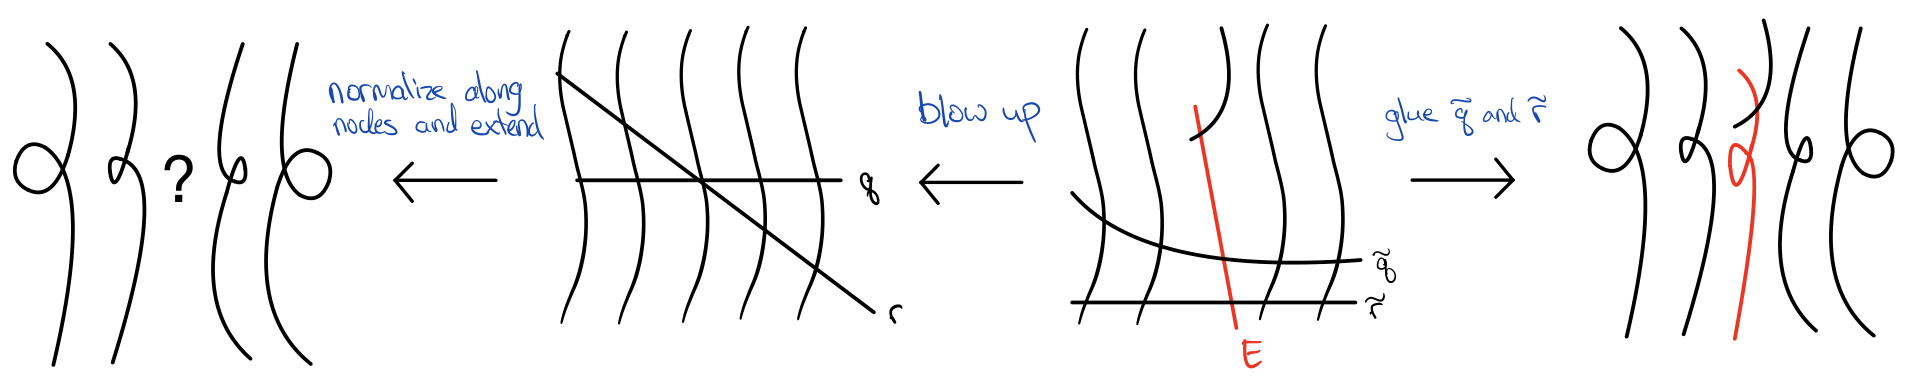
\includegraphics[width=.86\textwidth]{figures/reduction-step1.png}};
\begin{scope}[x={(im.south east)},y={(im.north west)}]
\fill[white] (0.17,0.62) rectangle (0.29,0.84);
\fill[white] (0.47,0.65) rectangle (0.56,0.8);
\fill[white] (0.72,0.64) rectangle (0.83,0.8);
\node[fill=white,inner sep=1pt,font=\scriptsize,text=blue] at (0.23,0.75) {沿结点正规化};
\node[fill=white,inner sep=1pt,font=\scriptsize,text=blue] at (0.23,0.64) {并延拓};
\node[fill=white,inner sep=1pt,font=\scriptsize,text=blue] at (0.514,0.7) {爆破};
\node[fill=white,inner sep=1pt,font=\scriptsize,text=blue] at (0.774,0.7) {粘合 $\widetilde q,\widetilde r$};
\end{scope}\end{tikzpicture}

\caption{(步骤 $1$) 考虑具有一个结点的稳定曲线族 $\mathcal C^*\to\Delta^*$, 例如由 $y^2=x^3+tx^2$ 局部定义的结点退化为尖点. 沿结点正规化, 延拓 $2$-点曲线族, 在截面 $q$, $r$ 的交点处爆破, 再粘合严格变换 $\widetilde q$, $\widetilde r$, 即得稳定极限. 若正规化 $\widetilde{\mathcal C}^*=C\times\Delta^*$ 是常值族, 则稳定极限是 $C$ 与一条有理结点曲线的结点并.}\label{src:6.5.3-figure}
\end{figure}\endgroup\addtocounter{theorem}{-1}
另一种归结方式是利用 $\mathcal M_{g,\allowbreak n}\subseteq\overline{\mathcal M}_{g,\allowbreak n}$ 稠密 (定理~\bookref{6.7.30}): 习题~\bookref{5.6.7} 断言, 只需在 $\Delta^*\to\overline{\mathcal M}_{g,\allowbreak n}$ 经过 $\mathcal M_{g,\allowbreak n}$ 分解的条件下检验固有性的赋值判据.

\textbf{步骤 $2$: 找到平坦延拓 $(\mathcal C\to\Delta,\allowbreak \sigma_i)$.}
由 $(\omega_{\mathcal C^*/\Delta^*}(\sum_i\sigma_i^*))^{\otimes3}$ 甚丰沛 (命题~\bookref{6.3.23}), 可将 $\mathcal C^*$ 嵌入为 $\mathbb P^N\times\Delta^*$ 的闭子概形. 由光滑曲线上的平坦性判据 (\bookref{A.2.2}), $\mathcal C^*\hookrightarrow\mathbb P^N\times\Delta$ 的概形论像 $\mathcal C$ 在 $\Delta$ 上平坦 (因为取闭包不会在中心纤维中引入嵌入点). 这给出延拓 $\mathcal C^*\to\Delta^*$ 的曲线族 $\mathcal C\to\Delta$. (这与命题~\bookref{2.4.2} 中用赋值判据证明 Hilbert 概形固有性的论证相同.) 由固有性的赋值判据 (\bookref{A.4.5}), 截面 $\sigma_i^*: \Delta^*\to\mathcal C^*$ 延拓为截面 $\sigma_i:\Delta\to\mathcal C$.

此时中心纤维 $\mathcal C_0$ 可能具有很严重的奇点, 标记点 $\sigma_i(0)\in\mathcal C_0$ 可能是奇点且彼此重合.
\begin{figure}[H]\centering\begin{tikzpicture}
\node[inner sep=0,anchor=south west] (im) at (0,0) {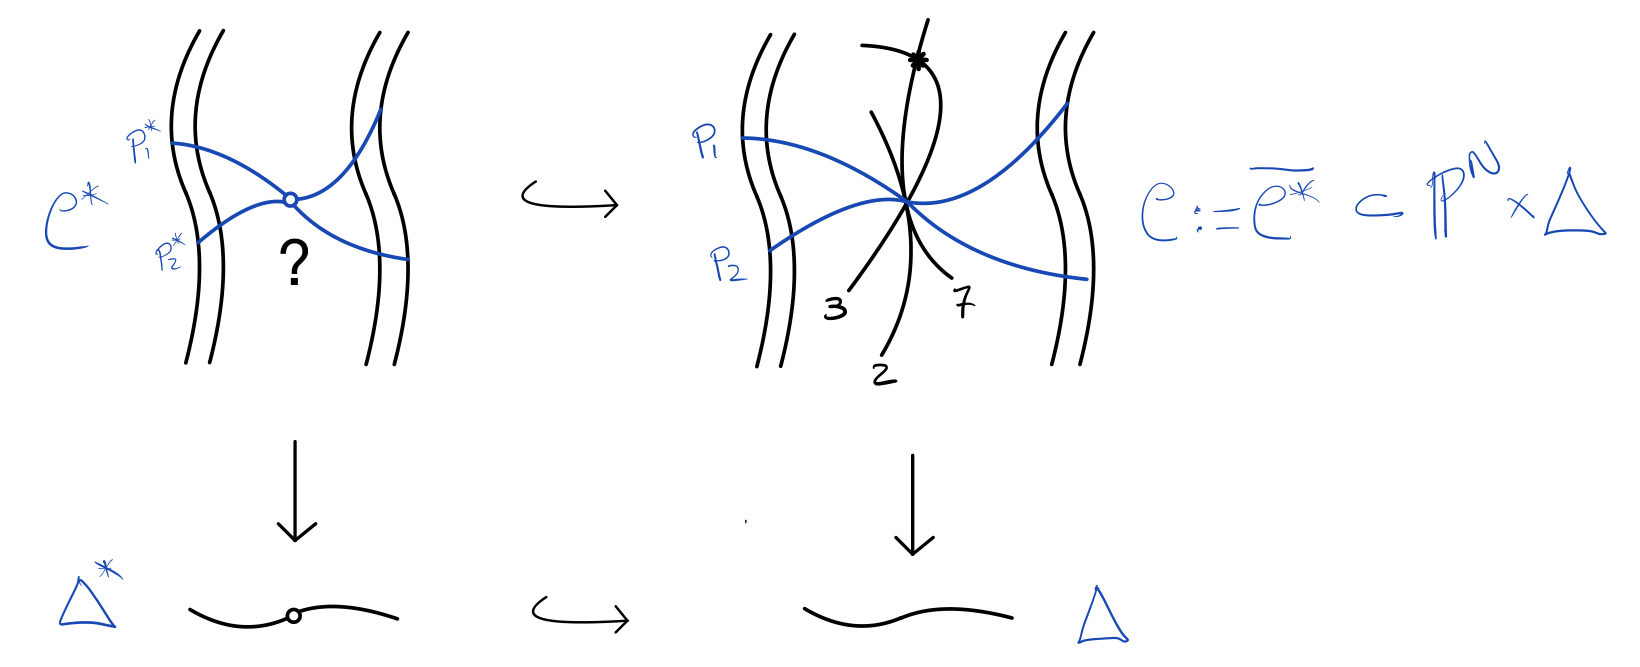
\includegraphics[width=.86\textwidth]{figures/reduction-step2.png}};
\begin{scope}[x={(im.south east)},y={(im.north west)}]


\end{scope}\end{tikzpicture}
\bookfiguretarget{6.5.4}
\caption{(步骤 $2$) 闭包 $\mathcal C:=\overline{\mathcal C^*}$ 是 $\Delta$ 上的平坦族. 中心纤维 $\mathcal C_0$ 可能一般非约化并带有嵌入点; 数字 $3$, $2$, $7$ 表示不可约分支的重数. 标记点 $\sigma_i(0)\in\mathcal C_0$ 可能是奇点且彼此重合.}\bookfigurehref{6.5.4}\label{src:6.5.4}
\end{figure}
\textbf{步骤 $3$: 将 $\mathcal C$ 换为奇点消解, 使约化中心纤维 $(\mathcal C_0)_{\mathrm{red}}$ 仅有结点.}
结合消解的存在性 (\bookref{B.2.1}) 与嵌入消解的存在性 (\bookref{B.2.3}), 存在从正则概形出发的射影双有理态射 $\widetilde{\mathcal C}\to\mathcal C$, 它在 $\Delta^*$ 上是同构, 且中心纤维 $\widetilde{\mathcal C}_0$ 在集合意义下具有正规交叉, 即 $(\widetilde{\mathcal C}_0)_{\mathrm{red}}$ 仅有结点. 由光滑曲线上的平坦性判据 (\bookref{A.2.2}), $\widetilde{\mathcal C}\to\Delta$ 平坦. 将 $\mathcal C$ 换为 $\widetilde{\mathcal C}$, 截面 $\sigma_i$ 换为严格变换.
\begin{figure}[H]\centering\begin{tikzpicture}
\node[inner sep=0,anchor=south west] (im) at (0,0) {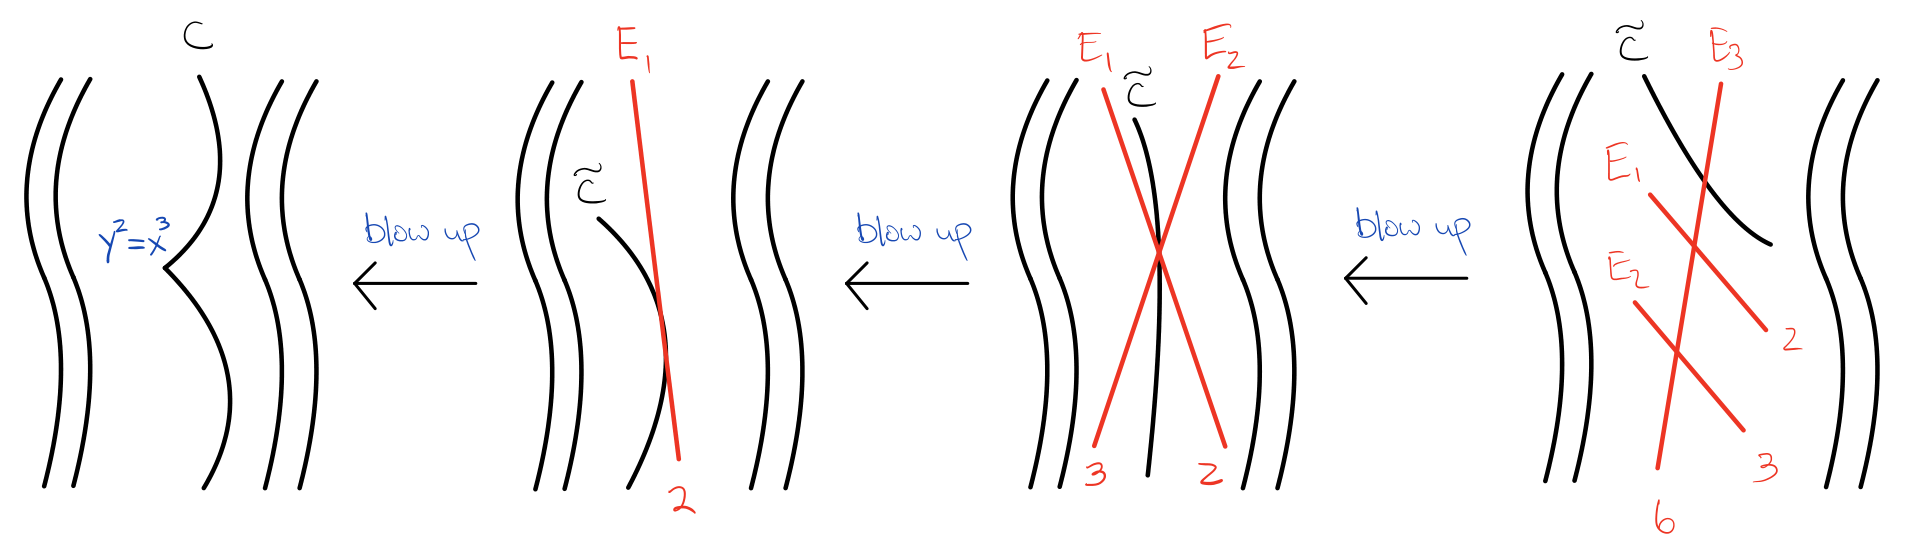
\includegraphics[width=.86\textwidth]{figures/reduction-step3.png}};
\begin{scope}[x={(im.south east)},y={(im.north west)}]
\fill[white] (0.185,0.52) rectangle (0.26,0.65);
\fill[white] (0.44,0.52) rectangle (0.52,0.65);
\fill[white] (0.7,0.52) rectangle (0.78,0.65);
\node[fill=white,inner sep=1pt,font=\scriptsize,text=blue] at (0.21,0.59) {爆破};
\node[fill=white,inner sep=1pt,font=\scriptsize,text=blue] at (0.477,0.59) {爆破};
\node[fill=white,inner sep=1pt,font=\scriptsize,text=blue] at (0.737,0.59) {爆破};
\end{scope}\end{tikzpicture}

\caption{(步骤 $3$) 设 $\mathcal C\to\Delta=\Bbbk[t]_{(t)}$ 是一般光滑的族, 中心纤维退化出尖点 $y^2=x^3$, 且 $\mathcal C$ 在该奇点附近的局部方程为 $y^2=x^3+t$. 反复爆破中心纤维的奇点, 在原曲面上取局部坐标 $x,\allowbreak y$, 在新曲面上取 $\widetilde x,\allowbreak \widetilde y$. 爆破的第一个坐标片中 $\widetilde x=x$, $\widetilde y=y/x$, 例外除子为 $\widetilde x=0$; 第二个坐标片中 $\widetilde x=x/y$, $\widetilde y=y$, 例外除子为 $\widetilde y=0$.}\label{src:6.5.5}
\end{figure}
\begin{itemize}
\item 第一次爆破中, 奇点在第一个坐标片中的原像由 $\widetilde x^2(\widetilde y^2-\widetilde x)$ 给出, 在第二个坐标片中由 $\widetilde y^2(1-\widetilde x^3\widetilde y)$ 给出. 例外除子 $E_1$ 的重数为 $2$. $C$ 的正规化 $\widetilde C$ 的亏格为 $g-1$.
\item 第二次爆破的坐标片由 $\widetilde x^3(\widetilde x\widetilde y^3-1)$ 和 $\widetilde x^2\widetilde y^3(\widetilde y-\widetilde x)$ 定义, 新例外除子 $E_2$ 的重数为 $3$.
\item 最后一次爆破的坐标片为 $\widetilde x^6\widetilde y^3(\widetilde y-1)$ 和 $\widetilde x^2\widetilde y^6(1-\widetilde x)$, 新例外除子 $E_3$ 的重数为 $6$. 中心纤维非约化, 其约化仅有结点.
\end{itemize}
\textbf{步骤 $4$: 作分歧基扩张 $\Delta'=\Spec R'\to\Spec R=\Delta$, 使 $\mathcal C\times_\Delta\Delta'$ 的正规化的中心纤维约化且仅有结点.}
这是最困难的步骤, 特征 $0$ 的假设用在这里. 此论证可看作 Abhyankar 温和分歧引理的一个版本 (见~\cite[\S XIII.5]{SGA1} 和~\cite[Tag 0EXT]{SP}). 因为 $\mathcal C$ 正则, $t\in R$ 不是零因子, 中心纤维 $\mathcal C_0$ 是 Cohen--Macaulay 的, 因而无嵌入点. 另一方面, $(\mathcal C_0)_{\mathrm{red}}$ 是有效 Cartier 除子, 局部由单个方程切出. 对每个 $p\in\mathcal C_0$, 可取平展邻域及局部坐标 $x,\allowbreak y$, 使 $\mathcal C\to\Delta$ 明确描述如下:
\begin{itemize}
\item 若 $p\in(\mathcal C_0)_{\mathrm{red}}$ 是光滑点, 则 $(x,\allowbreak y)\mapsto x^a$, 包含 $p$ 的不可约分支的重数为 $a$;
\item 若 $p\in(\mathcal C_0)_{\mathrm{red}}$ 是结点, 则 $(x,\allowbreak y)\mapsto x^ay^b$, 包含 $p$ 的两个分支的重数为 $a$, $b$. 若 $p$ 是非分离结点 (即 $\mathcal C_0\setminus p$ 连通), 则 $a=b$.
\end{itemize}
令 $N$ 为 $\mathcal C_0$ 的不可约分支重数的最小公倍数. 将 $R$ 换为扩张后, 可假设 $R$ 含有本原 $N$ 次单位根 $\rho$. 令 $\Delta'=\Spec R'\to\Spec R=\Delta$ 为 $N$ 次全分歧离散赋值环扩张 (即一致化参数 $t\in R$ 的像为 $t'^N$, 其中 $t'\in R'$ 是一致化参数). 令 $\mathcal C'=\mathcal C\times_\Delta\Delta'$, $p'\in\mathcal C'$ 为 $p$ 的唯一原像, $\widetilde{\mathcal C}'$ 为 $\mathcal C'$ 的正规化.

若 $p\in(\mathcal C_0)_{\mathrm{red}}$ 光滑, 则 $\mathcal C'$ 在 $p'$ 附近平展局部由 $x^a=t^N$ 定义. 因为 $R$ 的特征为 $0$, 有互异因子分解
\[
x^a-t^N=\prod_{i=0}^{a-1}\bigl(x-(\rho^it)^{N/a}\bigr).
\]
(若特征为正且整除 $N$, 则 $\mathcal C'$ 非约化.) 在正规化 $\widetilde{\mathcal C}'$ 中, 点 $p$ 有 $a$ 个原像, 各自平展局部由 $x=\rho^it^{N/a}$ 定义. 每个原像都是总族 $\widetilde{\mathcal C}'$ 和中心纤维 $\widetilde{\mathcal C}'_0$ 的光滑点. 若 $p$ 是结点, 则 $\mathcal C'$ 在 $p'$ 附近平展局部由 $x^ay^b=t^N$ 定义. 令 $d=\gcd(a,\allowbreak b)$. 若 $d>1$, 则有因子分解 (再次用到特征 $0$ 的假设)
\[
x^ay^b-t^N=\prod_{i=0}^{d-1}\bigl(x^{a/d}y^{b/d}-(\rho^it)^{N/d}\bigr).
\]
在 $p$ 附近平展局部, 正规化分解为 $\widetilde{\mathcal C}'\to\mathcal C''\to\mathcal C'$, 使 $p$ 在 $\mathcal C''$ 中有 $d$ 个原像, 各由 $x^{a/d}y^{b/d}-(\rho^it)^{N/d}$ 描述. 除非 $d=a=b$, 中心纤维 $\mathcal C''_0$ 仍非约化. 约化 $(\mathcal C''_0)_{\mathrm{red}}$ 在每个原像处有结点, 但两个分支的重数已互素. 因而可假设 $\gcd(a,\allowbreak b)=1$. 必要时交换 $x,\allowbreak y$, 可对正整数 $\alpha,\allowbreak \beta$ 写成 $1=\alpha a-\beta b$. 整环 $R[x,\allowbreak y]/(x^ay^b-t^N)$ 的正规化为
\[
R[x,y]/(x^ay^b-t^N)\hookrightarrow R[u,v]/(uv-t^{N/(ab)}),
\qquad x\mapsto u^b,\quad y\mapsto v^a,
\]
其中 $u=t^{\alpha N/b}/(x^\beta y^\alpha)$, $v=x^\beta y^\alpha/t^{\beta N/a}$. 中心纤维 $\widetilde{\mathcal C}'_0$ 约化, 在 $p$ 的唯一原像处有结点. 若 $N=ab$, 则 $\widetilde{\mathcal C}'$ 在此原像处光滑; 否则具有 $A_{n-1}$-奇点, 其中 $n=N/(ab)$.

现在中心纤维已约化且仅有结点, 但总族中出现了 $A_{n-1}$-奇点 (即 $xy-t^n$). 反复爆破每个 $A_{n-1}$-奇点, 将其换为 $\lfloor n/2\rfloor$ 条光滑有理曲线的结点并; 这明确描述了定理~\bookref{B.2.2} 中 $\widetilde{\mathcal C}'$ 的极小消解. 将 $\mathcal C$ 换为极小消解, 使总族 $\mathcal C$ 正则, 中心纤维 $\mathcal C_0$ 约化且仅有结点.
\begin{figure}[H]\centering\begin{tikzpicture}
\node[inner sep=0,anchor=south west] (im) at (0,0) {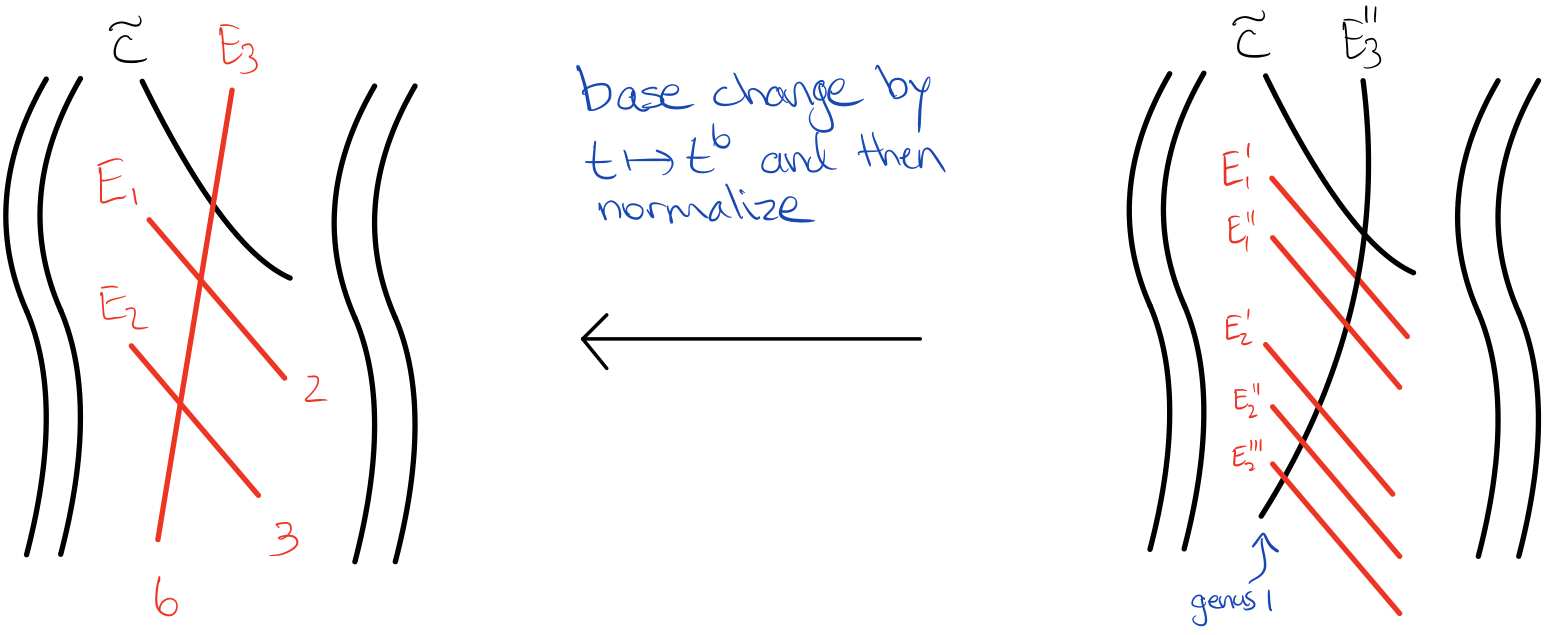
\includegraphics[width=.86\textwidth]{figures/reduction-step4.png}};
\begin{scope}[x={(im.south east)},y={(im.north west)}]
\fill[white] (0.36,0.63) rectangle (0.62,0.91);
\fill[white] (0.75,0.015) rectangle (0.83,0.1);
\node[fill=white,inner sep=1pt,font=\scriptsize,text=blue] at (0.5,0.83) {沿 $t\mapsto t^6$};
\node[fill=white,inner sep=1pt,font=\scriptsize,text=blue] at (0.5,0.71) {基变换并正规化};
\node[fill=white,inner sep=1pt,font=\scriptsize,text=blue] at (0.8,0.035) {亏格 $1$};
\end{scope}\end{tikzpicture}

\caption{(步骤 $4$) 接续图~\bookref{6.5.5}, 沿 $t\mapsto t^6$ 给出的 $\Delta'=\Spec\Bbbk[t]_{(t)}\to\Spec\Bbbk[t]_{(t)}=\Delta$ 对 $\mathcal C\to\Delta$ 作基变换, 再正规化. 中心纤维现已约化且仅有结点. $E_1$ 和 $E_2$ 的每个原像都是光滑有理曲线, $E_3$ 的原像 $E''_3$ 则是亏格 $1$ 曲线. 为理解此描述, 可将基变换分解为 $t\mapsto t^2$ 和 $t\mapsto t^3$ 的正规化基变换的复合; 见例~\bookref{6.5.13}.}\label{src:6.5.6}
\end{figure}
\textbf{步骤 $5$: 使标记点 $\sigma_i(0)\in\mathcal C_0$ 光滑且互异.}
反复爆破中心纤维 $\mathcal C_0$ 中标记点 $\sigma_i(0)$ 为奇点或相互碰撞的闭点, 则截面的严格变换成为中心纤维的互异光滑点. 将 $\mathcal C$ 换为爆破, 截面 $\sigma_i$ 换为严格变换后, 得到总族正则的预稳定族 $(\mathcal C\to\Delta,\allowbreak \sigma_i)$.
\begin{figure}[H]\centering\begin{tikzpicture}
\node[inner sep=0,anchor=south west] (im) at (0,0) {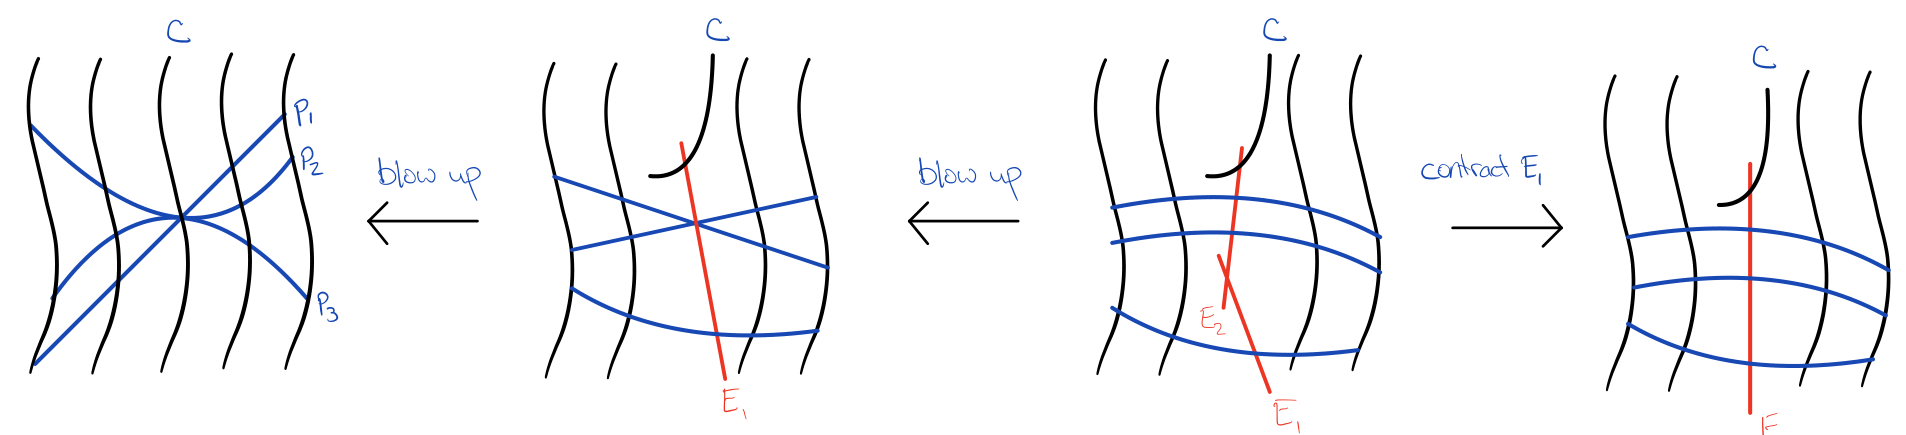
\includegraphics[width=.86\textwidth]{figures/reduction-step5.png}};
\begin{scope}[x={(im.south east)},y={(im.north west)}]
\fill[white] (0.18,0.52) rectangle (0.27,0.73);
\fill[white] (0.46,0.52) rectangle (0.55,0.73);
\fill[white] (0.74,0.52) rectangle (0.83,0.73);
\node[fill=white,inner sep=1pt,font=\scriptsize,text=blue] at (0.223,0.6) {爆破};
\node[fill=white,inner sep=1pt,font=\scriptsize,text=blue] at (0.506,0.6) {爆破};
\node[fill=white,inner sep=1pt,font=\scriptsize,text=blue] at (0.779,0.6) {收缩 $E_1$};
\end{scope}\end{tikzpicture}

\caption{(步骤 $5$) 考虑常值族 $C\times\Delta\to\Delta$, 截面局部为 $(\sigma_1,\allowbreak \sigma_2,\allowbreak \sigma_3)=(t^2,\allowbreak -t^2,\allowbreak 4t)$. 爆破两次后截面互不相交, 但中心纤维不稳定, 因为例外分支 $E_1\cong\mathbb P^1$ 仅有一个结点和一个标记点. 下一步将说明, 收缩有理桥 $E_1$ 即得稳定极限.}\label{src:6.5.7}
\end{figure}
\textbf{步骤 $6$: 收缩中心纤维中的有理尾和有理桥.}
预稳定族 $(\mathcal C\to\Delta,\allowbreak \sigma_i)$ 的中心纤维 $\mathcal C_0$ 稳定, 除非它含有有理尾或有理桥 (见定义~\bookref{6.3.12}). 若 $E\subseteq\mathcal C_0$ 是有理尾或带标记点的有理桥, 则 $E^2=-1$; 若 $E$ 是不带标记点的有理桥, 则 $E^2=-2$ (见注记~\bookref{6.3.16}). 由习题~\bookref{6.3.17}, 收缩每条有理尾和有理桥得到 $\Delta$ 上结点曲线族的态射 $\mathcal C\to\mathcal C'$. 令 $\sigma_i':\Delta\xrightarrow{\sigma_i}\mathcal C\to\mathcal C'$, 则 $n$-点曲线族 $(\mathcal C'\to\Delta,\allowbreak \sigma_i')$ 已经稳定! 也可用预稳定族的稳定收缩 (\bookref{6.6.6}) 构造此稳定族.
\end{proof}
\begin{figure}[H]\centering\begin{tikzpicture}
\node[inner sep=0,anchor=south west] (im) at (0,0) {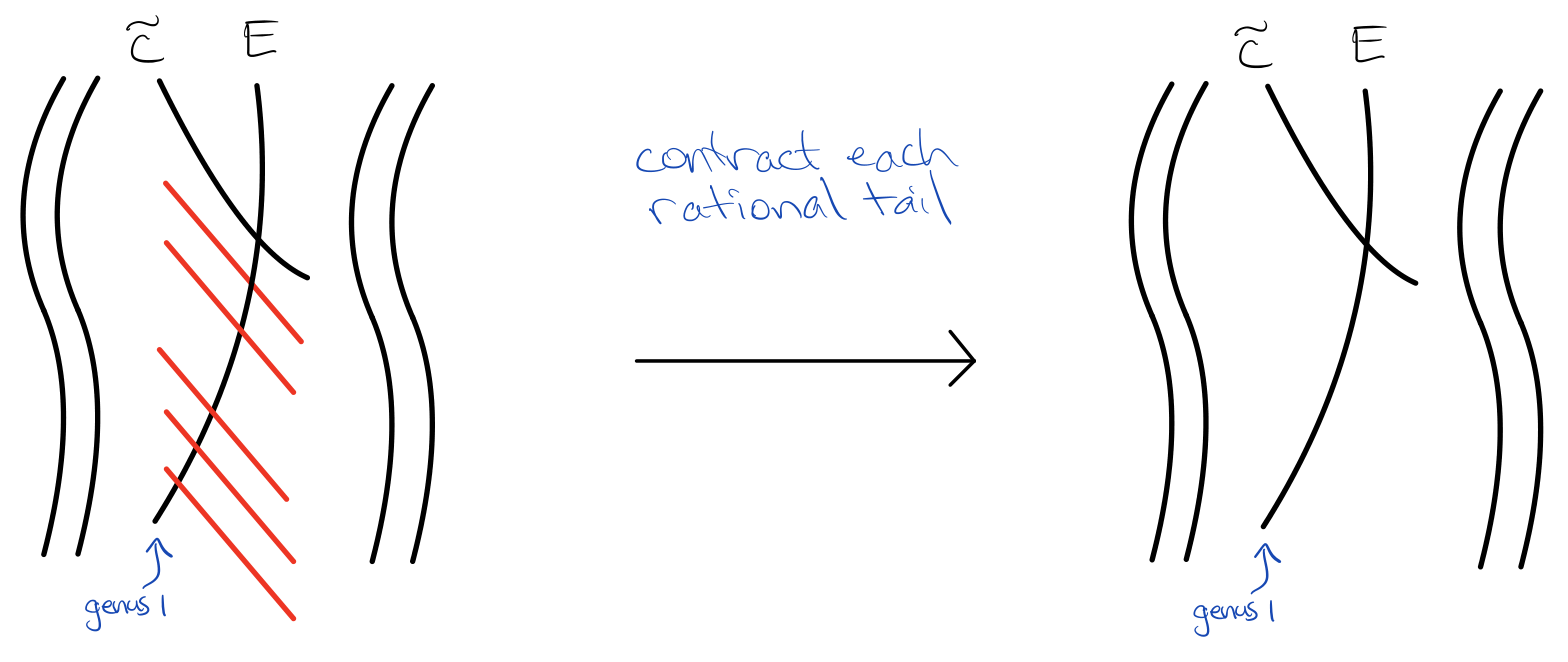
\includegraphics[width=.86\textwidth]{figures/reduction-step6.png}};
\begin{scope}[x={(im.south east)},y={(im.north west)}]
\fill[white] (0.37,0.62) rectangle (0.64,0.86);
\fill[white] (0.045,0.005) rectangle (0.13,0.085);
\fill[white] (0.75,0.005) rectangle (0.83,0.085);
\node[fill=white,inner sep=1pt,font=\scriptsize,text=blue] at (0.51,0.79) {收缩每条};
\node[fill=white,inner sep=1pt,font=\scriptsize,text=blue] at (0.51,0.7) {有理尾};
\node[fill=white,inner sep=1pt,font=\scriptsize,text=blue] at (0.085,0.055) {亏格 $1$};
\node[fill=white,inner sep=1pt,font=\scriptsize,text=blue] at (0.8,0.055) {亏格 $1$};
\end{scope}\end{tikzpicture}

\caption{(步骤 $6$) 接续图~\bookref{6.5.6}, 收缩每条红色有理尾得到稳定族. 中心纤维是原中心纤维 (带尖点) 的正规化 $\widetilde C$ 与椭圆曲线 $E$ 的结点并.}\label{src:6.5.8}
\end{figure}
若进行上述六步, 但在步骤 $6$ 中只收缩有理尾而保留有理桥, 则 Castelnuovo 收缩定理 (\bookref{B.2.6}) 保证总族仍正则. 这一重要变体称为\newterm{半稳定约化}{semistable reduction}.
\begin{theorem}[半稳定约化]\label{src:6.5.9}
设 $R$ 是离散赋值环, $K=\operatorname{Frac}(R)$, 并置 $\Delta=\Spec R$, $\Delta^*=\Spec K$. 若 $(\mathcal C^*\to\Delta^*,\allowbreak s_1^*,\allowbreak \ldots,\allowbreak s_n^*)$ 是 $n$-点\emph{光滑}曲线族, 则存在离散赋值环扩张 $R\to\allowbreak R'$ 及总族 $\mathcal C$ \emph{正则}的 $n$-点半稳定曲线族 $(\mathcal C\to\Delta'=\Spec R',\allowbreak s_1,\allowbreak \ldots,\allowbreak s_n)$, 延拓 $(\mathcal C^*\to\Delta^*,\allowbreak s_1^*,\allowbreak \ldots,\allowbreak s_n^*)$ 到 $K'=\operatorname{Frac}R'$ 的基变换.
\end{theorem}
\begin{remark}[特征 $p$ 下的证明]\label{src:6.5.10}
若 $R$ 的剩余域具有特征 $p>0$, 且中心纤维某些分支的重数被 $p$ 整除, 则上述稳定约化证明在步骤 $4$ 失效. 正特征下需要另一方法. 消解 $\mathcal C$ 的奇点并使 $(\mathcal C_0)_{\mathrm{red}}$ 仅有结点后 (如步骤 $3$), Artin 和 Winters 使 $\operatorname{Pic}(\mathcal C_{K'}^*)$ 的 $l$-挠子群对于充分大的素数 $l\ne p$ 同构于 $(\mathbb Z/l\mathbb Z)^{2g}$, 并证明这竟然迫使中心纤维约化且仅有结点! 见~\cite{AW71}, \cite[\S10.4]{Liu02} 和~\cite[Tag 0C2P]{SP}.
\end{remark}
\begin{example}[基变换必不可少]\label{src:6.5.11}
图~\bookref{6.5.5}, \bookref{6.5.6}, \bookref{6.5.8} 中尖点的稳定约化说明必须允许扩张离散赋值环. 事实上, 步骤 $3$ 后有一般光滑的族 $\mathcal C\to\Delta$, 总族 $\mathcal C$ 正则, 中心纤维 $\mathcal C_0$ 非约化. 假设存在稳定族 $\mathcal C'\to\Delta$, 使 $\mathcal C'|_{\Delta^*}\cong\mathcal C|_{\Delta^*}$. 消解 $\mathcal C'$ 的 $A_n$-奇点后, 有半稳定族 $\mathcal C''\to\Delta$, 其中 $\mathcal C''$ 正则, $\mathcal C''_0$ 半稳定 (特别地约化). 因为 $\mathcal C$ 与 $\mathcal C''$ 双有理, 取有理映射 $\mathcal C\dashrightarrow\mathcal C'$ 的图的闭包的奇点消解, 得到正则二维概形 $\mathcal D$ 和 $\Delta$ 上的双有理态射 $\mathcal D\to\mathcal C$, $\mathcal D\to\mathcal C''$. 由双有理映射的分解 (\bookref{B.2.4}), 每个态射分解为爆破的复合. 但 $\mathcal C$ 的任何爆破的中心纤维都非约化, $\mathcal C''$ 的任何爆破的中心纤维都约化, 这导致矛盾.
\end{example}
\subsection{显式稳定约化}\label{src:6.5.2-subsection}
在曲线几何的应用中, 常需明确描述稳定极限. 稳定约化的证明提供了策略, 但要得出显式描述还需仔细处理. 主要困难是确定步骤 $4$ 中全分歧扩张 $\Delta'\to\Delta$ 所给基变换 $\mathcal C'=\mathcal C\times_\Delta\Delta'$ 的正规化 $\widetilde{\mathcal C}'$. 常将 $\Delta'\to\Delta$ 分解为素数次基变换的复合更简单, 因为素数次正规化基变换 $\widetilde{\mathcal C}'\to\mathcal C$ 的分歧轨迹容易确定.
\begin{proposition}\label{src:6.5.12}
设 $p$ 是素数, $\mathcal C\to\Delta=\Spec R$ 是一般光滑的曲线族, 其中 $R$ 是含有 $p$ 次单位根的特征 $0$ 离散赋值环. 假设约化中心纤维 $(\mathcal C_0)_{\mathrm{red}}$ 仅有结点. 作为 $\mathcal C$ 上的除子, 写 $\mathcal C_0=\sum m_iD_i$, 其中 $m_i$ 是不可约分支 $D_i$ 的重数. 令 $\Delta'=\Spec R'\to\Spec R=\Delta$ 为 $p$ 次全非分歧扩张, 并置 $\mathcal C'=\mathcal C\times_\Delta\Delta'$, 正规化为 $\widetilde{\mathcal C}'$. 则 $\widetilde{\mathcal C}'\to\mathcal C$ 沿 $D_i$ 分歧当且仅当 $m_i$ 与 $p$ 互素. 若 $q'\in\widetilde{\mathcal C}'_0$ 是 $q\in D_i$ 的原像, 且 $q$ 是 $(\mathcal C_0)_{\mathrm{red}}$ 的光滑点, 则 $\widetilde{\mathcal C}'_0$ 在 $q'$ 附近的重数在 $p\mid m_i$ 时为 $m_i/p$, 否则为 $m_i$.
\end{proposition}
\begin{proof}
点 $q\in\mathcal C$ 有平展邻域和局部坐标 $x,\allowbreak y$, 使 $\mathcal C\to\Delta$ 描述为 $(x,\allowbreak y)\mapsto x^{m_i}$. 基变换 $\mathcal C'$ 在 $q'$ 附近平展局部描述为 $\Spec\Bbbk[x,\allowbreak y,\allowbreak t]/(x^{m_i}-t^p)$. 若 $p\mid m_i$, 则
\[
x^{m_i}-t^p=\prod_{i=0}^{p-1}(x^{m_i/p}-\rho^it),
\qquad\rho\text{ 为 }p\text{ 次单位根},
\]
其正规化有 $p$ 个光滑分支. 中心纤维 $\widetilde{\mathcal C}'_0$ 在 $q$ 的每个原像附近的重数为 $m_i/p$. 若 $m_i=pm'_i+r$, $0<r<p$, 则 $\Bbbk[x,\allowbreak y,\allowbreak t]/(x^{m_i}-t^p)$ 是整环, 正规化为
\[
\Bbbk[x,y,t']/(x^r-t'^p),\qquad t'=t/x^{m'_i}.
\]
所以 $\widetilde{\mathcal C}'\to\mathcal C$ 在 $q$ 处分歧. 中心纤维 $\widetilde{\mathcal C}'\to\Delta$ 由 $t=t'x^{m'_i}$ 定义, 在 $q$ 的唯一原像处的重数可计算为 $\dim_{\Bbbk}\Bbbk[x,\allowbreak t']/(x^r-t'^p,\allowbreak t'x^{m'_i})$. 因为 $t'^ix^j$ ($i=0,\allowbreak \ldots,\allowbreak p-1$, $j=0,\allowbreak \ldots,\allowbreak m'_i-1$) 与 $x^{m'_i},\allowbreak \ldots,\allowbreak x^{m'_i+r-1}$ 的并组成一组基, 重数为 $m_i$.
\end{proof}
\begin{example}[尖点的稳定约化]\label{src:6.5.13}
设 $\mathcal C\to\Delta=\Spec\Bbbk[t]_{(t)}$ 是一般光滑的族, 中心纤维 $C:=\mathcal C_0$ 退化出尖点 $y^2=x^3$, 且 $\mathcal C$ 在该奇点附近的局部方程为 $y^2=x^3+t$. 如图~\bookref{6.5.5} 所述, 对 $\mathcal C$ 作三次爆破, 得到族 $\mathcal C'\to\Delta$, 使 $(\mathcal C'_0)_{\mathrm{red}}$ 是正规化 $\widetilde C$ 与三个例外分支 $E_1,\allowbreak E_2,\allowbreak E_3$ 的结点并, 重数分别为 $1,\allowbreak 2,\allowbreak 3,\allowbreak 6$.
\end{example}
\begin{figure}[H]\centering\begin{tikzpicture}
\node[inner sep=0,anchor=south west] (im) at (0,0) {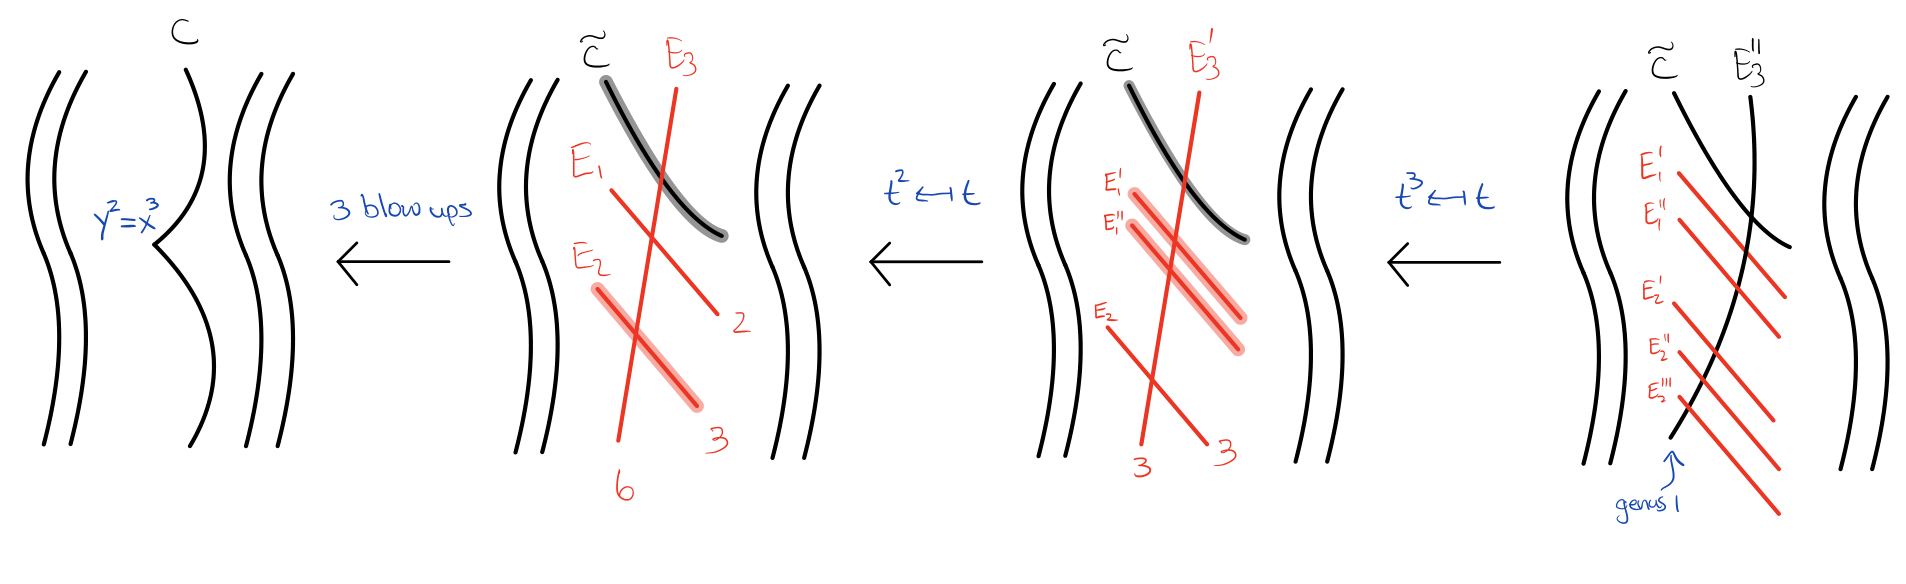
\includegraphics[width=.86\textwidth]{figures/reduction-cusp.png}};
\begin{scope}[x={(im.south east)},y={(im.north west)}]
\fill[white] (0.165,0.61) rectangle (0.26,0.75);
\fill[white] (0.46,0.62) rectangle (0.56,0.77);
\fill[white] (0.73,0.62) rectangle (0.81,0.77);
\fill[white] (0.845,0.09) rectangle (0.915,0.17);
\node[fill=white,inner sep=1pt,font=\scriptsize,text=blue] at (0.216,0.65) {$3$ 次爆破};
\node[fill=white,inner sep=1pt,font=\scriptsize,text=blue] at (0.5,0.675) {$t\mapsto t^2$};
\node[fill=white,inner sep=1pt,font=\scriptsize,text=blue] at (0.77,0.675) {$t\mapsto t^3$};
\node[fill=white,inner sep=1pt,font=\scriptsize,text=blue] at (0.88,0.13) {亏格 $1$};
\end{scope}\end{tikzpicture}

\caption{数字表示分支重数; 未标数字时重数为 $1$. 加粗分支表示正规化基变换的分歧轨迹.}\label{src:6.5.14}
\end{figure}
由命题~\bookref{6.5.12}, 第一次正规化基变换 $t\mapsto t^2$ 的分歧轨迹是 $\widetilde C$ 与 $E_2$ 的并. $E_1$ 的原像是两条光滑有理曲线的不交并 $E'_1\amalg E''_1$. $E_3$ 的原像 $E'_3$ 是在两点处分歧的 $E_3=\mathbb P^1$ 的二重覆盖, 所以 $E'_3=\mathbb P^1$, 但此时重数为 $2$. 第二次正规化基变换的分歧轨迹为 $\widetilde C\amalg E'_1\amalg E''_1$ (再次由命题~\bookref{6.5.12}). $E_2$ 的原像是三条光滑有理曲线的并, $E'_3$ 的原像 $E''_3$ 是 $E'_3=\mathbb P^1$ 的光滑三重覆盖, 在三点处分歧, 每点的分歧指数均为二. 由 Riemann--Hurwitz (\bookref{6.7.4}), $E''_3$ 的亏格 $g_{E''_3}$ 为 $1$:
\[
2g_{E''_3}-2=3(2(0)-2)+3(2)=0.
\]
最后如图~\bookref{6.5.8} 收缩五条有理尾, 稳定极限是光滑亏格 $g-1$ 曲线 $\widetilde C$ (原中心纤维的正规化) 与亏格 $1$ 曲线的结点并 $\widetilde C\cup E''_3$.
\begin{remark}\label{src:6.5.15}
稳定极限中究竟出现哪条椭圆曲线 $E''_3$, 稳定极限如何依赖退化的选择? 尖点的形变空间为 $y^2=x^3+a_1(t)x+a_0(t)$; 换言之, 问题是稳定极限如何依赖 $a_i(t)$. 例如, 若曲面的总族有奇点 (如 $y^2=x^{2k+1}+t^2$), 会发生什么? \cite[\S3.C]{HM98} 详细讨论了这些问题.
\end{remark}
\newpage
\begin{exercise}[很好的练习]\label{src:6.5.16}
\begin{enumerate}[(a)]
\item 求一般光滑的族退化出密切结点 $y^2=x^4$ 时的稳定极限.
\item 更一般地, 证明一般光滑的族退化出 $A_{2k}$-奇点 $y^2=x^{2k+1}$ (分别地, $y^2=x^{2k+2}$) 时, 稳定极限是亏格 $g-k$ 曲线与亏格 $k$ 超椭圆曲线的结点并, 在一个 Weierstrass 点 (分别地, 两个 Weierstrass 共轭点) 处粘接. 超椭圆曲线 $H$ 的 Weierstrass 点是二重覆盖 $H\to\mathbb P^1$ 的分歧点; 两点为 Weierstrass 共轭点是指它们的并是 $H\to\mathbb P^1$ 的一个纤维.
\end{enumerate}
\end{exercise}
\begin{example}[二重二次曲线的稳定约化]\label{src:6.5.17}
考虑一般光滑的族 $\mathcal C\to\Delta=\Spec\Bbbk[t]_{(t)}$, 其中 $\mathcal C\subseteq\mathbb P^2\times\Delta$ 由 $F^2+tG$ 定义, $F$ 是光滑二次曲线, $G$ 是光滑四次曲线. 中心纤维是 $F^2$ 定义的二重二次曲线. 总空间在 $F\cap G$ 的 $8$ 个交点 $p_1,\allowbreak \ldots,\allowbreak p_8$ 处各有一个局部方程为 $x^2+yt$ 的 $A_1$-奇点. 每个 $\sigma_i$ 经一次爆破消解, 例外除子 $E_i=\mathbb P^1$ 的重数为 $1$. 得到族 $\mathcal C_2\to\Delta$, 中心纤维作为除子为 $2C+\sum_iE_i$. 随后取分歧覆盖 $\Delta'\to\Delta$, $t\mapsto t^2$ 所给基变换 $\mathcal C_2\times_\Delta\Delta'$ 的正规化 $\mathcal C_3$. 由命题~\bookref{6.5.12}, $\mathcal C_3\to\mathcal C_2$ 沿 $E_i$ 的不交并分歧. $C$ 的原像是 $\mathbb P^1$ 的二重覆盖, 在 $8$ 个点 $\sigma_i$ 处分歧, 因而是光滑亏格 $3$ 超椭圆曲线.
\end{example}
\begin{figure}[H]\centering\begin{tikzpicture}
\node[inner sep=0,anchor=south west] (im) at (0,0) {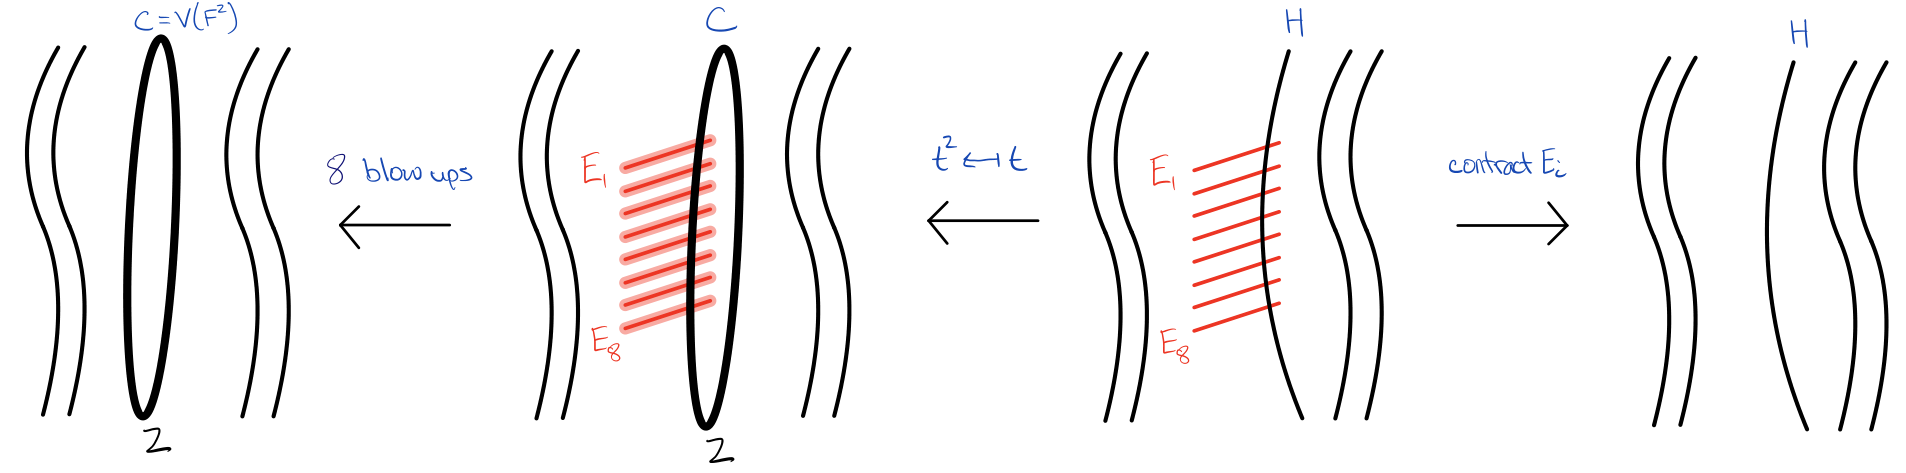
\includegraphics[width=.86\textwidth]{figures/reduction-double-conic.png}};
\begin{scope}[x={(im.south east)},y={(im.north west)}]
\fill[white] (0.16,0.58) rectangle (0.28,0.72);
\fill[white] (0.48,0.57) rectangle (0.56,0.72);
\fill[white] (0.74,0.57) rectangle (0.84,0.74);
\node[fill=white,inner sep=1pt,font=\scriptsize,text=blue] at (0.228,0.62) {$8$ 次爆破};
\node[fill=white,inner sep=1pt,font=\scriptsize,text=blue] at (0.5,0.62) {$t\mapsto t^2$};
\node[fill=white,inner sep=1pt,font=\scriptsize,text=blue] at (0.772,0.62) {收缩 $E_i$};
\end{scope}\end{tikzpicture}

\caption{退化为二重二次曲线 $C=V(F^2)$ 的一般光滑族 $F^2+tG$ 的稳定约化.}\label{src:6.5.18}
\end{figure}
\begin{exercise}[元习题]\label{src:6.5.19}
阅读~\cite[\S3.C]{HM98} 的论述并完成其中的习题.
\end{exercise}
\subsection{\texorpdfstring{$\overline{\mathcal M}_{g,\allowbreak n}$ 的固有性}{稳定曲线模叠 的固有性}}\label{src:6.5.3-subsection}
稳定约化 (\bookref{6.5.1}) 蕴涵 $\overline{\mathcal M}_{g,\allowbreak n}$ 的固有性赋值判据中的存在性部分. 还需证明稳定极限唯一, 即 $\overline{\mathcal M}_{g,\allowbreak n}$ 分离.
\begin{proposition}\label{src:6.5.20}
设 $R$ 是离散赋值环, $K=\operatorname{Frac}(R)$, 并置 $\Delta=\Spec R$, $\Delta^*=\Spec K$. 若 $(\mathcal C\to\Delta,\allowbreak \sigma_1,\allowbreak \ldots,\allowbreak \sigma_n)$ 和 $(\mathcal D\to\Delta,\allowbreak \tau_1,\allowbreak \ldots,\allowbreak \tau_n)$ 是 $n$-点稳定曲线族, 则 $\Delta^*$ 上每个与截面的限制相容 (即 $\tau_i^*=\alpha^*\circ\sigma_i^*$) 的同构 $\alpha^*:\mathcal C\times_\Delta\Delta^*\to\mathcal D\times_\Delta\Delta^*$, 均延拓为唯一的 $\Delta$ 上同构 $\alpha:\mathcal C\to\mathcal D$, 满足 $\tau_i=\alpha\circ\sigma_i$.
\end{proposition}
\begin{proof}
为简单起见, 处理无标记点 ($n=0$) 的情形. 先断言可归结到一般纤维 $\mathcal C^*\cong\mathcal D^*$ 在 $\Delta^*$ 上光滑, 其中 $\mathcal C^*=\mathcal C\times_\Delta\Delta^*$. 采用稳定约化 (\bookref{6.5.1}) 证明的步骤 $1$ 中归结到一般光滑情形的同一策略. 由平坦下降, 只需在离散赋值环扩张 $\Delta'\to\Delta$ 后构造 $\alpha:\mathcal C\to\mathcal D$; 事实上, 同构 $\alpha':\mathcal C\times_\Delta\Delta'\to\mathcal D\times_\Delta\Delta'$ 因 $\mathcal D\to\Delta$ 分离而满足余圈条件, 从而下降为同构 $\alpha$. 因而可假设 $\mathcal C^*\cong\mathcal D^*$ 的每个结点由 $K$-点给出, 在正规化下的原像为两个 $K$-点. 每个结点延拓为截面 $\Delta\to\mathcal C$, $\Delta\to\mathcal D$. 带标记的正规化 $\widetilde{\mathcal C}$, $\widetilde{\mathcal D}$ 各为带标记稳定族的不交并. 若 $\mathcal C^*\to\mathcal D^*$ 延拓为同构 $\widetilde\alpha:\widetilde{\mathcal C}\to\widetilde{\mathcal D}$, 则 $\alpha$ 下降为同构 $\mathcal C\to\mathcal D$. 或者利用 $\mathcal M_{g,\allowbreak n}\subseteq\overline{\mathcal M}_{g,\allowbreak n}$ 稠密 (稍后定理~\bookref{6.7.30} 证明), 只需在 $\Delta^*\to\overline{\mathcal M}_{g,\allowbreak n}$ 经过 $\mathcal M_{g,\allowbreak n}$ 分解的条件下检验分离性的赋值判据 (习题~\bookref{5.6.7}).

令 $\widetilde{\mathcal C}\to\mathcal C$ 和 $\widetilde{\mathcal D}\to\mathcal D$ 为极小消解 (定理~\bookref{B.2.2}). 令 $\Gamma$ 为 $(\mathrm{id},\allowbreak \alpha^*):\mathcal C^*\to\widetilde{\mathcal C}\times_\Delta\widetilde{\mathcal D}$ 的像的闭包, $\widetilde\Gamma\to\Gamma$ 为其极小消解. 得到交换图
\begin{equation}\label{src:6.5.21}
\begin{tikzcd}[column sep=small,row sep=small]
&\widetilde{\mathcal C}\arrow[r]&\mathcal C\arrow[dr]&\\
\widetilde\Gamma\arrow[ur]\arrow[dr]&&&\Delta\\
&\widetilde{\mathcal D}\arrow[r]&\mathcal D\arrow[ur]&
\end{tikzcd}
\end{equation}
给出两种论证说明存在延拓 $\alpha^*$ 的同构 $\alpha:\mathcal C\to\mathcal D$. 第一种: $\mathcal C$ (分别地 $\mathcal D$) 在中心纤维的结点附近的局部结构是形如 $xy=t^{n+1}$ 的 $A_n$-奇点, 其中 $t\in R$ 是一致化参数. 每个结点在 $\widetilde{\mathcal C}\to\mathcal C$ (分别地 $\widetilde{\mathcal D}\to\mathcal D$) 下的原像是有理桥链 $E_1\cup\cdots\cup E_n$, $E_i^2=-2$. 因为 $\mathcal C$, $\mathcal D$ 是稳定曲线族, 它们不含光滑有理 $-1$ 曲线, 所以 $\widetilde{\mathcal C}$, $\widetilde{\mathcal D}$ 也不含这样的曲线. 由双有理映射的分解 (定理~\bookref{B.2.4}), $\widetilde\Gamma\to\widetilde{\mathcal C}$ 和 $\widetilde\Gamma\to\widetilde{\mathcal D}$ 都是有限次闭点爆破的复合. 因为 $\widetilde\Gamma\to\Gamma$ 是极小消解, $\widetilde\Gamma$ 不含同时被两个态射收缩的光滑有理 $-1$ 曲线. 断言这两个态射都是同构. 这将完成证明, 因为 $\mathcal C$, $\mathcal D$ 均由收缩 $\widetilde{\mathcal C}\cong\widetilde{\mathcal D}$ 的光滑有理 $-2$ 曲线得到.

为证断言, 假设例如 $\widetilde\Gamma\to\widetilde{\mathcal C}$ 不是同构. 则存在不被 $\widetilde\Gamma\to\widetilde{\mathcal D}$ 收缩的光滑有理 $-1$ 曲线 $E\subseteq\widetilde\Gamma$. 令 $E_{\widetilde{\mathcal D}}\subseteq\widetilde{\mathcal D}$ 为它的像. 爆破只会减小自交数 (事实上, 若 $E_{\widetilde{\mathcal D}}$ 在 $\Gamma$ 中的原像写成 $E+F$, 则投影公式给出 $E_{\widetilde{\mathcal D}}^2=E\cdot(E+F)=E^2+E\cdot F$), 所以 $E_{\mathcal D}^2\geq E^2=-1$. 另一方面, 例外曲线的 Hodge 指数定理 (\bookref{B.2.5}) 给出 $E_{\mathcal D}^2\leq-1$. 因而 $E_{\mathcal D}^2=-1$. 但 $E_{\mathcal D}\subseteq\widetilde{\mathcal D}$ 不是光滑有理 $-1$ 曲线, 故必有奇点, 复合 $\widetilde\Gamma\to\widetilde{\mathcal D}$ 中某次爆破必在 $E_{\mathcal D}$ 的奇点处进行. 这意味着例外轨迹 $F$ 与 $E$ 非平凡相交, 从而 $E_{\mathcal D}^2\geq E^2+1$, 矛盾.

也可如下论证. 光滑射影曲面的双有理映射 $\widetilde\Gamma\to\widetilde{\mathcal C}$ 和 $\widetilde\Gamma\to\widetilde{\mathcal D}$ 在余维 $2$ 处是同构. 相对对偶化层是线丛, 因而对每个非负整数 $k$, 多重典范截面有认同
\[
\Gamma(\widetilde{\mathcal C},\omega_{\widetilde{\mathcal C}/\Delta}^{\otimes k})
\cong\Gamma(\widetilde\Gamma,\omega_{\widetilde\Gamma/\Delta}^{\otimes k})
\cong\Gamma(\widetilde{\mathcal D},\omega_{\widetilde{\mathcal D}/\Delta}^{\otimes k})
\]
(参见~\cite[定理 II.8.19]{Har77}). 由 $\mathcal C$, $\mathcal D$ 是 $\Delta$ 上族 $\widetilde{\mathcal C}$, $\widetilde{\mathcal D}$ 的稳定收缩 (定理~\bookref{6.6.6}), 即多重典范截面分次环的 $\operatorname{Proj}$, 得到延拓 $\alpha^*:\mathcal C^*\to\mathcal D^*$ 的同构
\[
\mathcal C\xrightarrow{\sim}\operatorname{Proj}\bigoplus_k\Gamma(\widetilde{\mathcal C},\omega_{\widetilde{\mathcal C}/\Delta}^{\otimes k})
\xrightarrow{\sim}\operatorname{Proj}\bigoplus_k\Gamma(\widetilde{\mathcal D},\omega_{\widetilde{\mathcal D}/\Delta}^{\otimes k})
\xrightarrow{\sim}\mathcal D.
\]
另见~\cite[引理 1.12]{DM69}, \cite[引理 10.5.1]{ACG11} 和~\cite[Tag 0E97]{SP}.
\end{proof}
\begin{exercise}[细节]\label{src:6.5.22}
将上述证明推广到有标记点的情形.
\end{exercise}
虽然我们只在特征 $0$ 下证明了稳定约化 (\bookref{6.5.1}), 仍在 $\mathbb Z$ 上陈述下一个结果.
\begin{theorem}[$\overline{\mathcal M}_{g,\allowbreak n}$ 和 $\overline M_{g,\allowbreak n}$ 的固有性]\label{src:6.5.23}
若 $2g-2+n>0$, 则 Deligne--Mumford 叠 $\overline{\mathcal M}_{g,\allowbreak n}$ 在 $\Spec\mathbb Z$ 上固有. 此外, 存在粗模空间 $\overline{\mathcal M}_{g,\allowbreak n}\to\overline M_{g,\allowbreak n}$, 其中 $\overline M_{g,\allowbreak n}$ 是 $\Spec\mathbb Z$ 上固有的代数空间.
\end{theorem}
\begin{proof}
因为 $\overline{\mathcal M}_{g,\allowbreak n}$ 拟分离 (习题~\bookref{6.4.18}), 可应用固有性的赋值判据 (\bookref{4.8.7}). 稳定约化 (\bookref{6.5.1}) 给出极限的存在性, 命题~\bookref{6.5.20} 给出唯一性. 因为 $\overline{\mathcal M}_{g,\allowbreak n}$ 分离, Keel--Mori 定理 (\bookref{5.4.6}) 给出粗模空间 $\overline{\mathcal M}_{g,\allowbreak n}\to\overline M_{g,\allowbreak n}$, 其中 $\overline M_{g,\allowbreak n}$ 是 $\Spec\mathbb Z$ 上分离有限型的代数空间. 由于 $\overline{\mathcal M}_{g,\allowbreak n}$ 在 $\Spec\mathbb Z$ 上固有, $\overline M_{g,\allowbreak n}$ 也固有.
\end{proof}
\begin{exercise}\label{src:6.5.24}
证明 $\overline{\mathcal M}_{g,\allowbreak n}\times_{\mathbb Z}\mathbb F_p$ 的粗模空间是 $\overline M_{g,\allowbreak n}\times_{\mathbb Z}\mathbb F_p$ 的正规化.
\end{exercise}
\newpage
\begin{question}[未解决]\label{src:6.5.25}
$\overline M_{g,\allowbreak n}\times_{\mathbb Z}\mathbb F_p$ 是否为 $\overline{\mathcal M}_{g,\allowbreak n}\times_{\mathbb Z}\mathbb F_p$ 的粗模空间?\footnote{见 \url{https://mathoverflow.net/questions/9981/coarse-moduli-spaces-over-z-and-f-p} 和 \url{https://mathoverflow.net/questions/72903/what-is-m-g-over-a-finite-field-really}.}
\end{question}

% Source printed pp. 253-263 / PDF pp. 261-271.
\section{收缩, 遗忘与粘合态射}\label{src:6.6}
\begin{epigraph}
旧定理永不消亡; 它们化为定义.
\epigraphauthor{Edwin Hewitt}
\end{epigraph}
本节构造曲线模空间之间的若干重要态射.
\begin{itemize}
\item (稳定收缩) 态射 $\mathcal M_{g,\allowbreak n}^{\mathrm{pre}}\to\overline{\mathcal M}_{g,\allowbreak n}$ 将预稳定族 $(\mathcal C\to\allowbreak S,\allowbreak \sigma_i)$ 映为通过收缩所有有理尾和有理桥得到的稳定族 $(\mathcal C^{\mathrm{st}},\allowbreak \sigma_i^{\mathrm{st}})$ (定理~\bookref{6.6.6}).
\item (遗忘) 态射 $\overline{\mathcal M}_{g,\allowbreak n+1}\to\overline{\mathcal M}_{g,\allowbreak n}$ 将 $(n+1)$-点稳定族 $(\mathcal C\to\allowbreak S,\allowbreak \sigma_1,\allowbreak \ldots,\allowbreak \sigma_{n+1})$ 映为 $n$-点预稳定族 $(\mathcal C\to\allowbreak S,\allowbreak \sigma_1,\allowbreak \ldots,\allowbreak \sigma_n)$ 的稳定收缩 (命题~\bookref{6.6.10}). 此态射还是泛族 (命题~\bookref{6.6.12}).
\item (粘合) 态射 $\overline{\mathcal M}_{i,\allowbreak k}\times\overline{\mathcal M}_{g-i,\allowbreak n-k+2}\to\overline{\mathcal M}_{g,\allowbreak n}$ 沿最后的截面, 将亏格 $i$ 的 $k$-点稳定族与亏格 $g-i$ 的 $(n-k+2)$-点稳定族粘合; 态射 $\overline{\mathcal M}_{g-1,\allowbreak n+2}\to\overline{\mathcal M}_{g,\allowbreak n}$ 则粘合亏格 $g-1$ 的 $(n+2)$-点稳定族的最后两个截面 (推论~\bookref{6.6.16}).
\end{itemize}
与结点族的局部结构 (\bookref{6.2.26}) 一样, 最大的困难是保证这些构造适用于任意基底上的族. 本节最后在~\bookref{6.6.4-subsection} 节讨论 $\overline{\mathcal M}_{g,\allowbreak n}$ 上的边界除子和线丛.
\subsection{收缩有理尾和有理桥}\label{src:6.6.1-subsection}
域上预稳定曲线的有理尾和有理桥定义于定义~\bookref{6.3.12}, 其特征刻画见引理~\bookref{6.3.13}. 先证明域上的有理尾和有理桥可收缩为稳定曲线 (推论~\bookref{6.6.3}), 再将构造推广到族 (定理~\bookref{6.6.6}).
\begin{proposition}[收缩有理尾或有理桥]\label{src:6.6.1}
设 $(C,\allowbreak p_i)$ 是域 $k$ 上的 $n$-点预稳定曲线, $E$ 是有理尾或有理桥. 则存在典范态射 $c:C\to\allowbreak C'$, 将 $E$ 收缩为一点, 满足 $c_*\mathcal O_C=\mathcal O_{C'}$, $\mathrm R^1c_*\mathcal O_C=0$. 此外, $C'$ 可认同为推出 $\Spec\Gamma(E,\allowbreak \mathcal O_E)\amalg_E C$, $c:C\to\allowbreak C'$ 的构造与 $k$ 的域扩张交换.
\end{proposition}
\begin{proof}
两种情形下, 都将 $C'$ 构造为 Ferrand 推出 (\bookref{B.4.1})
\[
\begin{tikzcd}
E\cap E^c\arrow[r]\arrow[d]&E^c\arrow[d]\\
\Spec k'\arrow[r]\arrow[ur,phantom,"\lrcorner"]&C',
\end{tikzcd}
\qquad k'=\mathrm H^0(E,\mathcal O_E).
\]
因为概形论的并是推出 (习题~\bookref{B.4.6}), $C=E\amalg_{E\cap E^c}E^c$. 这诱导更大的交换图
\[
\begin{tikzcd}
E\cap E^c\arrow[r]\arrow[d]&E^c\arrow[d]\\
E\arrow[r]\arrow[d]&C\arrow[d,"c"]\\
\Spec k'\arrow[r]&C'.
\end{tikzcd}
\]
其中 $c:C\to\allowbreak C'$ 是使图交换的唯一映射. 上方和外侧方块都是推出, 所以下方方块也是推出, 即 $C'=\Spec k'\amalg_E C$. Ferrand 推出与域扩张交换 (命题~\bookref{B.4.8}(4)), 故 $c$ 的构造也如此.

若 $E$ 是有理尾或带标记点的有理桥, 则对点 $x\in E\cap E^c$ 有 $E\cap E^c=\Spec k'=\Spec\kappa(x)$ (见引理~\bookref{6.3.13}), 因而 $C'=E^c$. 映射 $c:C\to\allowbreak C'=E^c$ 在 $E^c$ 上为恒等, 并通过结构态射 $E\to\Spec\Gamma(E,\allowbreak \mathcal O_E)=\Spec\kappa(x)$ 将 $E$ 收缩到 $x\in E^c$. 考虑短正合列
\[
0\to\mathcal O_C\to\mathcal O_E\oplus\mathcal O_{E^c}\to\kappa(x)\to0.
\]
应用 $c_*$ 得到长正合列
\[
\begin{aligned}
0\to c_*\mathcal O_C\to i_{x,*}\widetilde{\mathrm H^0(E,\mathcal O_E)}\oplus\mathcal O_{C'}
\to\kappa(x)\to\mathrm R^1c_*\mathcal O_C\\
\to i_{x,*}\widetilde{\mathrm H^1(E,\mathcal O_E)}\to0,
\end{aligned}
\]
其中 $i_x:\Spec\kappa(x)\hookrightarrow C'$ 是 $x$ 的包含. 因为 $\mathrm H^0(E,\allowbreak \mathcal O_E)=\kappa(x)$, $\mathrm H^1(E,\allowbreak \mathcal O_E)=0$, 得到 $c_*\mathcal O_C=\mathcal O_{C'}$, $\mathrm R^1c_*\mathcal O_C=0$.

若 $E$ 是不带标记点的有理桥, 置 $k''=\mathrm H^0(E\cap E^c,\allowbreak \mathcal O_{E\cap E^c})$. 由引理~\bookref{6.3.13}, $E\cap E^c$ 或者是一个点, $k''$ 为 $k'$ 的 $2$ 次可分扩张, 或者是两个点, $k''=k'\times k'$. 因为推出构造是平展局部的 (命题~\bookref{B.4.8}(3)), 仿射推出
\[
\begin{tikzcd}[column sep=small]
\Spec k''\arrow[r,"0"]\arrow[d]&\Spec k''[y]\arrow[d]\\
\Spec k'\arrow[r]\arrow[ur,phantom,"\lrcorner"]&\Spec\{f\in k''[y]\mid f(0)\in k'\}
\end{tikzcd}
\]
和
\[
\begin{tikzcd}
\Spec(k'\times k')\arrow[r,"0\amalg0"]\arrow[d]&\Spec(k'[y]\times k'[z])\arrow[d]\\
\Spec k'\arrow[r]\arrow[ur,phantom,"\lrcorner"]&\Spec k'[y,z]/(yz)
\end{tikzcd}
\]
分别在 $E\cap E^c$ 为一个或两个点时, 给出 $C$ 在 $E$ 的像处的平展邻域. 两种情形下 $E$ 的像都是结点. 如上利用短正合列 $0\to\mathcal O_C\to\mathcal O_E\oplus\mathcal O_{E^c}\to\mathcal O_{E\cap E^c}\to0$, 可证 $c_*\mathcal O_C=\mathcal O_{C'}$, $\mathrm R^1c_*\mathcal O_C=0$. 另见~\cite[Tags 0E3H, 0E3M]{SP}.
\end{proof}
曲线还可包含任意长度的有理尾和有理桥链.
\begin{figure}[H]\centering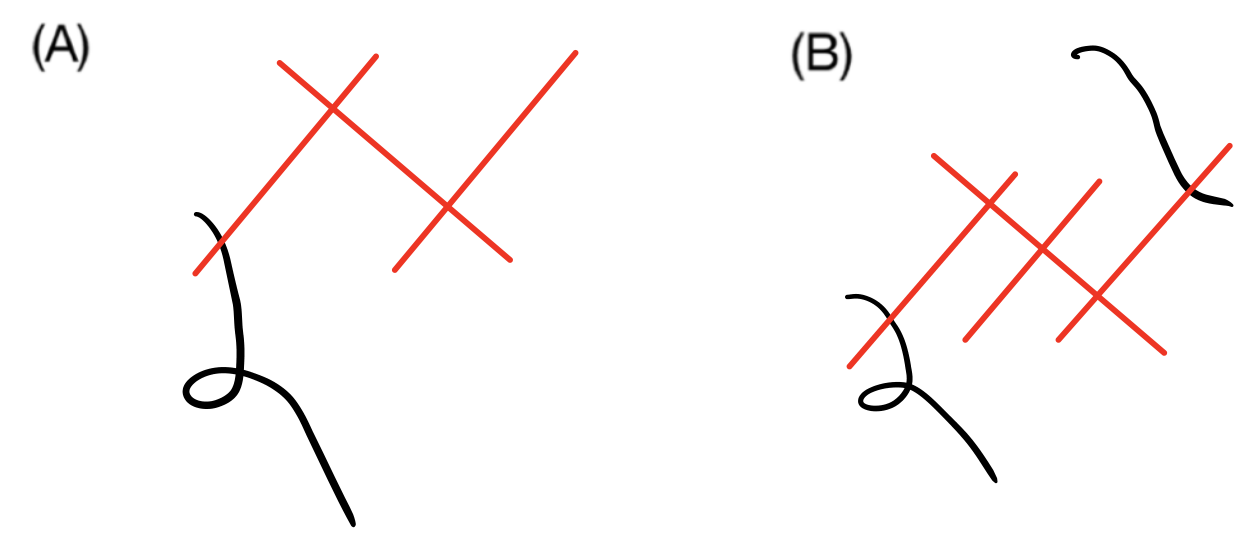
\includegraphics[width=.6\textwidth]{figures/fig-6.6.2.png}
\caption{有理尾和有理桥链.}\label{src:6.6.2}\end{figure}
\begin{corollary}[稳定收缩]\label{src:6.6.3}
设 $(C,\allowbreak p_i)$ 是域 $k$ 上亏格 $g$ 的 $n$-点预稳定曲线, $2g-2+n>0$. 则存在典范态射 $c:C\to\allowbreak C^{\mathrm{st}}$, 称为\newterm{稳定收缩}{stable contraction}, 将所有有理尾和有理桥收缩为点, 使 $(C^{\mathrm{st}},\allowbreak c(p_i))$ 为亏格 $g$ 的 $n$-点稳定曲线, $c_*\mathcal O_C=\mathcal O_{C^{\mathrm{st}}}$, $\mathrm R^1c_*\mathcal O_C=0$. 此外, $c$ 的构造与 $k$ 的域扩张交换.
\end{corollary}
\begin{proof}
令 $E$ 为所有有理尾和有理桥的概形论并, 则 $\mathrm H^0(E,\allowbreak \mathcal O_E)$ 是有限个域的乘积. 反复应用命题~\bookref{6.6.1}, 得到推出图
\[
\begin{tikzcd}
E\arrow[r]\arrow[d]&C\arrow[d,"c"]\\
\Spec\mathrm H^0(E,\mathcal O_E)\arrow[r]\arrow[ur,phantom,"\lrcorner"]&C^{\mathrm{st}},
\end{tikzcd}
\]
满足 $c_*\mathcal O_C=\mathcal O_{C^{\mathrm{st}}}$, $\mathrm R^1c_*\mathcal O_C=0$, 且 $c$ 的构造与域扩张交换. 因为 $(C^{\mathrm{st}},\allowbreak c(p_i))$ 不含有理尾和有理桥, 它稳定 (命题~\bookref{6.3.15}). 另见~\cite[Tag 0E7Q]{SP}.
\end{proof}
\begin{figure}[H]\centering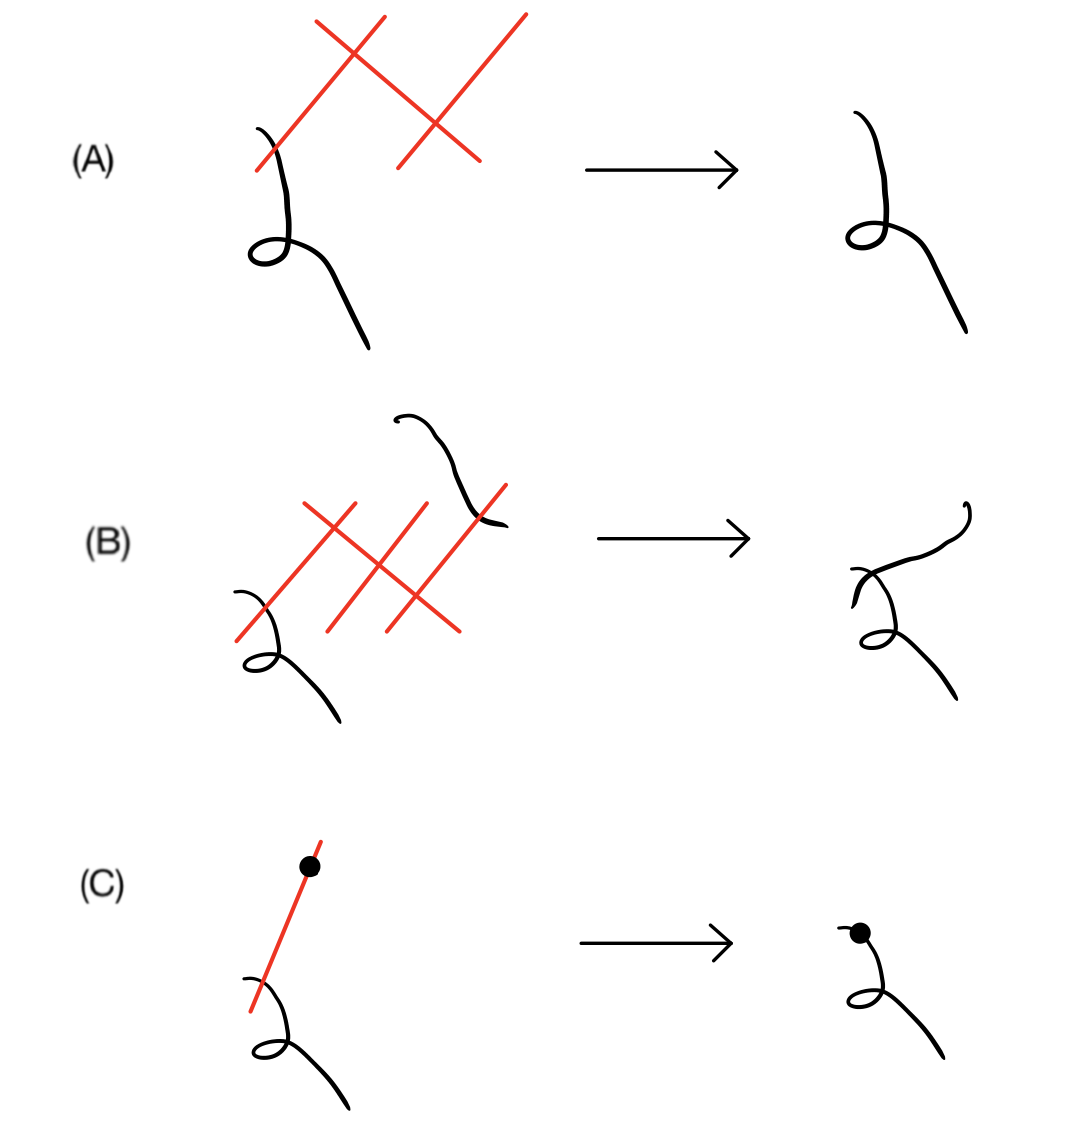
\includegraphics[width=.55\textwidth]{figures/fig-6.6.4.png}
\caption{稳定收缩.}\label{src:6.6.4}\end{figure}
\begin{exercise}\label{src:6.6.5}
设 $(C,\allowbreak p_i)$ 是域 $k$ 上的 $n$-点预稳定曲线.
\begin{enumerate}[(a)]
\item 证明稳定化态射 $c:C\to\allowbreak C^{\mathrm{st}}$ 是满足 $(C^{\mathrm{st}},\allowbreak c(p_i))$ 稳定, $c_*\mathcal O_C=\mathcal O_{C^{\mathrm{st}}}$, $\mathrm R^1c_*\mathcal O_C=0$ 的唯一态射.
\item 若 $(C,\allowbreak p_i)$ 半稳定, $L:=\omega_C(\sum_i p_i)$, 证明 $C^{\mathrm{st}}\cong\operatorname{Proj}\bigoplus_{d\geq0}\mathrm H^0(C,\allowbreak L^{\otimes d})$, 且 $L\cong c^*\omega_{C^{\mathrm{st}}}(\sum_i c(p_i))$.
\end{enumerate}
\end{exercise}
稳定收缩的构造可推广到预稳定曲线族.
\begin{theorem}[预稳定族的稳定收缩]\label{src:6.6.6}
若 $(\mathcal C\to\allowbreak S,\allowbreak \sigma_i)$ 是亏格 $g$ 的 $n$-点预稳定曲线族, $2g-2+n>0$, 则存在唯一的 $S$ 上态射 $c:\mathcal C\to\mathcal C^{\mathrm{st}}$, 使得
\begin{enumerate}[(1)]
\item $(\mathcal C^{\mathrm{st}}\to\allowbreak S,\allowbreak \sigma_i^{\mathrm{st}})$ 是亏格 $g$ 的 $n$-点稳定曲线族, 其中 $\sigma_i^{\mathrm{st}}=c\circ\sigma_i$;
\item $\mathcal O_{\mathcal C^{\mathrm{st}}}=c_*\mathcal O_{\mathcal C}$, $\mathrm R^1c_*\mathcal O_{\mathcal C}=0$;
\item $c:\mathcal C\to\mathcal C^{\mathrm{st}}$ 的构造与基变换 $S'\to\allowbreak S$ 相容;
\item 对每个 $s\in S$, $(\mathcal C_s,\allowbreak \sigma_i(s))\to(\mathcal C_s^{\mathrm{st}},\allowbreak \sigma_i^{\mathrm{st}}(s))$ 是推论~\bookref{6.6.3} 中有理桥和有理尾的稳定收缩.
\end{enumerate}
此外, 若 $(\pi:\mathcal C\to\allowbreak S,\allowbreak \sigma_i)$ 是半稳定族, 则 $\omega_{\mathcal C/S}(\sum_i\sigma_i)$ 是相对丰沛线丛 $L:=\omega_{\mathcal C^{\mathrm{st}}/S}(\sum_i\sigma_i^{\mathrm{st}})$ 的拉回; 特别地, $\mathcal C^{\mathrm{st}}\cong\operatorname{Proj}_S\bigoplus_{d\geq0}\pi_*(L^{\otimes d})$.
\end{theorem}
\begin{proof}
给出从局部到整体的论证. 对任意 $s\in S$, 推论~\bookref{6.6.3} 给出 $\kappa(s)$ 上的稳定收缩 $c_s:\mathcal C_s\to\allowbreak Y_0$, 由习题~\bookref{6.6.5}(a) 满足唯一性. 关键思想如下: 因为 $c_{s,\allowbreak *}\mathcal O_{\mathcal C_s}=\mathcal O_{Y_0}$, $\mathrm R^1c_{s,\allowbreak *}\mathcal O_{\mathcal C_s}=0$, $\mathcal C_s$ 的任意无穷小形变唯一延拓为 $\mathcal C_s\to\allowbreak Y_0$ 的形变 (习题~\bookref{C.2.9}). 置 $S_n=\Spec\mathcal O_{S,\allowbreak s}/\mathfrak m^{n+1}$, 得到 $S_n$ 上相容的态射
\[
\mathcal C\times_S S_n\to Y_n.
\]
Artin 逼近 (\bookref{B.5.18}) 在平展覆盖 $S'\to\allowbreak S$ 后给出态射 $\mathcal C\times_S S'\to\allowbreak Y'$, 由唯一性下降为 $\mathcal C\to\mathcal C^{\mathrm{st}}$.

为使此论证成立, 先用极限方法 (\bookref{B.3} 节) 归结到 $S$ 在 $\mathbb Z$ 上有限型. 如第一段, 找到 $S_n$ 上相容的态射 $\mathcal C\times_S S_n\to\allowbreak Y_n$. 由命题~\bookref{5.5.19}, 中心纤维 $\mathcal C_s$, $Y_0$ 是概形, 故 $\mathcal C\times_S S_n$, $Y_n$ 也是概形. 因为 $\widehat S:=\Spec\widehat{\mathcal O}_{S,\allowbreak s}$ 是 Noether 的, Grothendieck 存在定理 (推论~\bookref{C.5.8}) 给出射影态射 $\widehat Y\to\widehat S$, 延拓 $Y_n\to\allowbreak S_n$. 由平坦性的无穷小判据 (\bookref{A.2.5}), $\widehat Y\to\widehat S$ 平坦. Grothendieck 存在定理的推论 (\bookref{C.5.11}) 给出延拓 $\mathcal C\times_S S_n\to\allowbreak Y_n$ 的 $\widehat S$ 上态射 $\mathcal C\times_S\widehat S\to\widehat Y$. 令 $\widehat\tau_i$ 为复合 $\widehat S\xrightarrow{\sigma_i\times_S\widehat S}\mathcal C\times_S\widehat S\to\widehat Y$, 则 $(\widehat Y\to\widehat S,\allowbreak \widehat\tau_i)$ 是 $n$-点曲线族. 中心纤维 $Y_0$ 稳定, 故稳定性的开放性 (\bookref{6.3.24}) 保证它是稳定曲线族.

因为 $S$ 在 $\mathbb Z$ 上有限型, Artin 逼近 (\bookref{B.5.18}) 给出平展邻域 $(S',\allowbreak s')\to(S,\allowbreak s)$, 稳定曲线族 $(Y'\to\allowbreak S',\allowbreak \tau_i)$ 和 $S'$ 上代数空间的态射 $c':\mathcal C\times_S S'\to\allowbreak Y'$, 在 $s'$ 处的纤维对应于 $\mathcal C_s\to\allowbreak Y_0$. 由习题~\bookref{6.6.8}, 将 $S'$ 换为 $s'$ 的开邻域后, 可假设 $c_*\mathcal O_{\mathcal C\times_S S'}=\mathcal O_{Y'}$, $\mathrm R^1c_*\mathcal O_{\mathcal C\times_S S'}=0$, 且在基变换后仍成立. 一旦建立唯一性, 所需稳定曲线族的存在性便由平展下降得出.

为证唯一性, 设 $(Y\to\allowbreak S,\allowbreak \tau_i)$, $(Y'\to\allowbreak S,\allowbreak \tau'_i)$ 是稳定曲线族, $c:\mathcal C\to\allowbreak Y$, $c':\mathcal C\to\allowbreak Y'$ 是 $S$ 上态射, 并假设有与 $c_s$, $c'_s$ 相容的同构 $\alpha_s:Y_s\xrightarrow{\sim}Y'_s$, 且 $c_{s,\allowbreak *}\mathcal O_{\mathcal C_s}=\mathcal O_{Y_s}$, $\mathrm R^1c_{s,\allowbreak *}\mathcal O_{\mathcal C_s}=0$. 需证存在 $s$ 的开邻域 $U\subseteq S$ 和延拓 $\alpha_s$ 的同构 $\alpha:Y_U\to\allowbreak Y'_U$, 与 $c_U$, $c'_U$ 相容. 由极限方法 (\bookref{B.3} 节), 可假设 $S=\Spec A$, $A$ 为 Noether 局部环. 令 $Y''$ 为 $\mathcal C\to\allowbreak Y\times_S Y'$ 的概形论像, 只需证投影 $Y''\to\allowbreak Y$, $Y''\to\allowbreak Y'$ 为同构. 因为概形论像与平坦基变换交换, 还可假设 $A$ 完备. 由习题~\bookref{C.2.9}, 基变换到 $\Spec A/\mathfrak m^{n+1}$ 后的限制 $Y''_n\to\allowbreak Y_n$, $Y''_n\to\allowbreak Y'_n$ 都是同构. Grothendieck 存在定理的推论 (\bookref{C.5.11}) 给出所需同构 $Y\to\allowbreak Y'$. 另见~\cite[Tag 0E8A]{SP}.

若 $(\mathcal C\to\allowbreak S,\allowbreak \sigma_i)$ 是半稳定曲线族, 则断言自然映射 $c^*\omega_{\mathcal C^{\mathrm{st}}/S}\to\omega_{\mathcal C/S}$ 是同构. 相对对偶化层是线丛, 因而只需证此映射满射. 因为相对对偶化层和该映射的余核与基变换相容, 由 Nakayama 引理, 只需在 $S$ 为域的谱时证明断言, 这正是习题~\bookref{6.6.5}(b). 由投影公式, $\omega_{\mathcal C^{\mathrm{st}}/S}\cong c_*c^*\omega_{\mathcal C^{\mathrm{st}}/S}$, 从而复合 $\omega_{\mathcal C^{\mathrm{st}}/S}\cong c_*c^*\omega_{\mathcal C^{\mathrm{st}}/S}\to\allowbreak c_*\omega_{\mathcal C/S}$ 是同构. 因此
\[
\omega_{\mathcal C^{\mathrm{st}}/S}\Bigl(\sum_i\sigma_i^{\mathrm{st}}\Bigr)
\cong c_*\Bigl(\omega_{\mathcal C/S}\Bigl(\sum_i\sigma_i\Bigr)\Bigr),
\]
这由 $\omega_{\mathcal C^{\mathrm{st}}/S}$ 相对甚丰沛 (命题~\bookref{6.3.22}) 推出所述结论. 或者可通过证明自然映射 $\pi_*(L^{\otimes2})\otimes\pi_*(L^{\otimes d})\to\pi_*(L^{\otimes(d+2)})$ 对 $d\geq4$ 满射, 在整体上明确构造稳定收缩. 从而 $\bigoplus_{d\geq0}\pi_*(L^{\otimes4d})$ 是有限型 $\mathcal O_S$-代数, 可定义 $\mathcal C^{\mathrm{st}}:=\operatorname{Proj}_S\bigoplus_{d\geq0}\pi_*(L^{\otimes4d})$. 因为对所有 $d\geq0$, 推前 $\pi_*(L^{\otimes4d})$ 是向量丛, 其构造与基变换交换 (命题~\bookref{6.3.23}), $\mathcal C\to\mathcal C^{\mathrm{st}}$ 良定义, $\mathcal C^{\mathrm{st}}\to\allowbreak S$ 是稳定曲线族. 见~\cite[命题 2.1]{Knu83a} 和~\cite[命题 10.6.7]{ACG11}.
\end{proof}
\begin{corollary}[稳定收缩态射]\label{src:6.6.7}
存在代数叠的态射
\[
\mathcal M_{g,n}^{\mathrm{pre}}\to\overline{\mathcal M}_{g,n},\qquad
(C,p_i)\mapsto(C^{\mathrm{st}},c(p_i)),
\]
在开子叠 $\overline{\mathcal M}_{g,\allowbreak n}\subseteq\mathcal M_{g,\allowbreak n}^{\mathrm{pre}}$ 上为恒等.
\end{corollary}
\newpage
\begin{exercise}[细节]\label{src:6.6.8}
设 $f:X\to\allowbreak Y$ 是 Noether 概形 $S$ 上曲线族的态射. 假设对某点 $s\in S$, 态射 $f_s:X_s\to\allowbreak Y_s$ 满足 $f_{s,\allowbreak *}\mathcal O_{X_s}=\mathcal O_{Y_s}$, $\mathrm R^1f_{s,\allowbreak *}\mathcal O_{X_s}=0$. 证明将 $S$ 换为 $s$ 的开邻域后, 有 $f_*\mathcal O_X=\mathcal O_Y$, $\mathrm R^1f_*\mathcal O_X=0$, 且沿态射 $S'\to\allowbreak S$ 基变换后仍成立. 另见~\cite[Tag 0E88]{SP}.
\end{exercise}
\subsection{\texorpdfstring{遗忘态射与 $\overline{\mathcal M}_{g,\allowbreak n}$ 的泛族}{遗忘态射与 稳定曲线模叠 的泛族}}\label{src:6.6.2-subsection}
给出稳定收缩态射 (\bookref{6.6.7}) 的两个推论: 存在映射 $\overline{\mathcal M}_{g,\allowbreak n+1}\to\overline{\mathcal M}_{g,\allowbreak n}$, 它是在遗忘最后一个标记点之后的稳定收缩, 且可认同为泛族.
\begin{figure}[H]\centering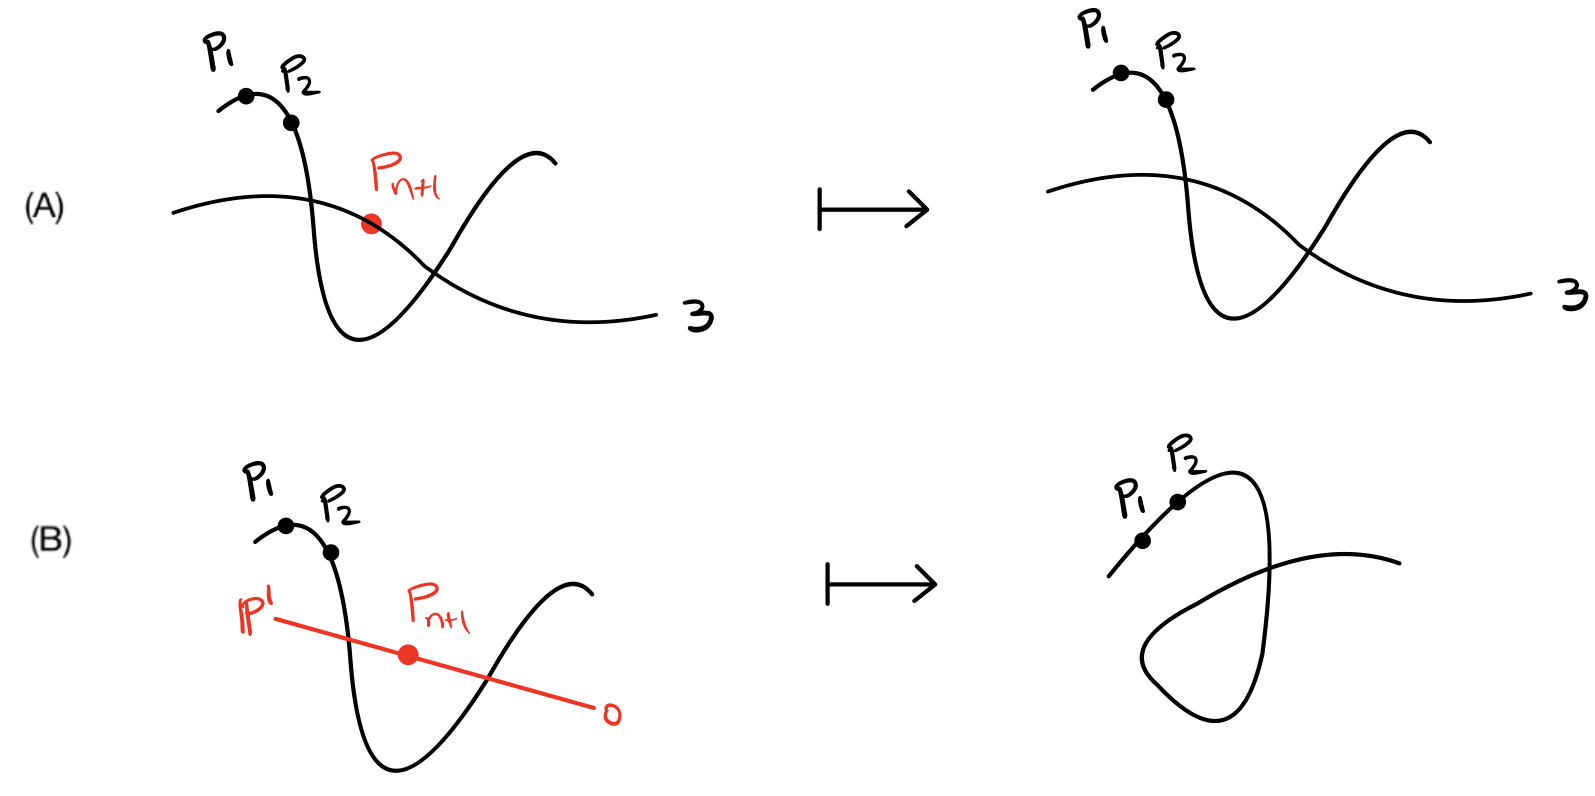
\includegraphics[width=.7\textwidth]{figures/fig-6.6.9.png}
\caption{(A) 中只需遗忘第 $n+1$ 个点. (B) 中若遗忘 $p_{n+1}$, 曲线不再稳定, 必须收缩有理桥.}\label{src:6.6.9}\end{figure}
\begin{proposition}[遗忘态射]\label{src:6.6.10}
存在代数叠的态射
\[
\overline{\mathcal M}_{g,n+1}\to\overline{\mathcal M}_{g,n},\qquad
(C,p_1,\ldots,p_{n+1})\mapsto(C^{\mathrm{st}},c(p_1),\ldots,c(p_n)),
\]
其中 $c:C\to\allowbreak C^{\mathrm{st}}$ 是 $(C,\allowbreak p_1,\allowbreak \ldots,\allowbreak p_n)$ 的稳定收缩.
\end{proposition}
\begin{proof}
所需态射构造为复合
\[
\overline{\mathcal M}_{g,n+1}\to\mathcal M_{g,n}^{\mathrm{pre}}\to\overline{\mathcal M}_{g,n},
\]
其中第一箭头将 $(n+1)$-点稳定族 $(\mathcal C\to\allowbreak S,\allowbreak \sigma_1,\allowbreak \ldots,\allowbreak \sigma_{n+1})$ 映为 $n$-点预稳定族 $(\mathcal C\to\allowbreak S,\allowbreak \sigma_1,\allowbreak \ldots,\allowbreak \sigma_n)$, 第二箭头是稳定收缩态射 (\bookref{6.6.7}).
\end{proof}
由广义 $2$-Yoneda 引理 (\bookref{4.1.27}), 恒等态射 $\overline{\mathcal M}_{g,\allowbreak n}\to\overline{\mathcal M}_{g,\allowbreak n}$ 对应于代数叠 $\overline{\mathcal M}_{g,\allowbreak n}$ 上的一个 $\overline{\mathcal M}_{g,\allowbreak n}$ 对象, 后者通过下降对应于 $n$-点稳定曲线族
\[
(\mathcal U_{g,n}\to\overline{\mathcal M}_{g,n},\sigma_1^{\mathrm{univ}},\ldots,\sigma_n^{\mathrm{univ}}),
\]
称为泛族. $\mathcal U_{g,\allowbreak n}$ 在概形 $S$ 上的对象是 $n$-点稳定曲线族 $(\mathcal C\to\allowbreak S,\allowbreak \sigma_i)$, 配备额外截面 $\tau:S\to\mathcal C$ (它可落入 $\mathcal C\to\allowbreak S$ 的结点轨迹, 也可与 $\sigma_i$ 非平凡相交). 给定 $n$-点稳定曲线族 $(\mathcal C\to\allowbreak S,\allowbreak \sigma_i)$, 存在在唯一同构意义下唯一的态射 $S\to\overline{\mathcal M}_{g,\allowbreak n}$ 及 Cartesian 图
\[
\begin{tikzcd}
\mathcal C\arrow[r]\arrow[d,shift right=1ex]&\mathcal U_{g,n}\arrow[d,shift right=1ex]\\
S\arrow[r]\arrow[u,shift right=1ex,"\sigma_i"]&\overline{\mathcal M}_{g,n}\arrow[u,shift right=1ex,"\sigma_i^{\mathrm{univ}}"'].
\end{tikzcd}
\]
另一方面, 有遗忘态射 (\bookref{6.6.10}) 和代数叠的态射 $\overline{\mathcal M}_{g,\allowbreak n+1}\to\mathcal U_{g,\allowbreak n}$, 将 $(n+1)$-点稳定族 $(\mathcal C\to\allowbreak S,\allowbreak \sigma_i)$ 映为 $(\mathcal C^{\mathrm{st}},\allowbreak \sigma_1^{\mathrm{st}},\allowbreak \ldots,\allowbreak \sigma_n^{\mathrm{st}},\allowbreak c\circ\sigma_{n+1})$, 其中 $c:\mathcal C\to\mathcal C^{\mathrm{st}}$ 是预稳定族 $(\mathcal C,\allowbreak \sigma_1,\allowbreak \ldots,\allowbreak \sigma_n)$ 的稳定收缩 (\bookref{6.6.6}). 得到交换图
\[
\begin{tikzcd}
\overline{\mathcal M}_{g,n+1}\arrow[rr]\arrow[dr]&&\mathcal U_{g,n}\arrow[dl]\\
&\overline{\mathcal M}_{g,n}.&
\end{tikzcd}
\]
\begin{figure}[H]\centering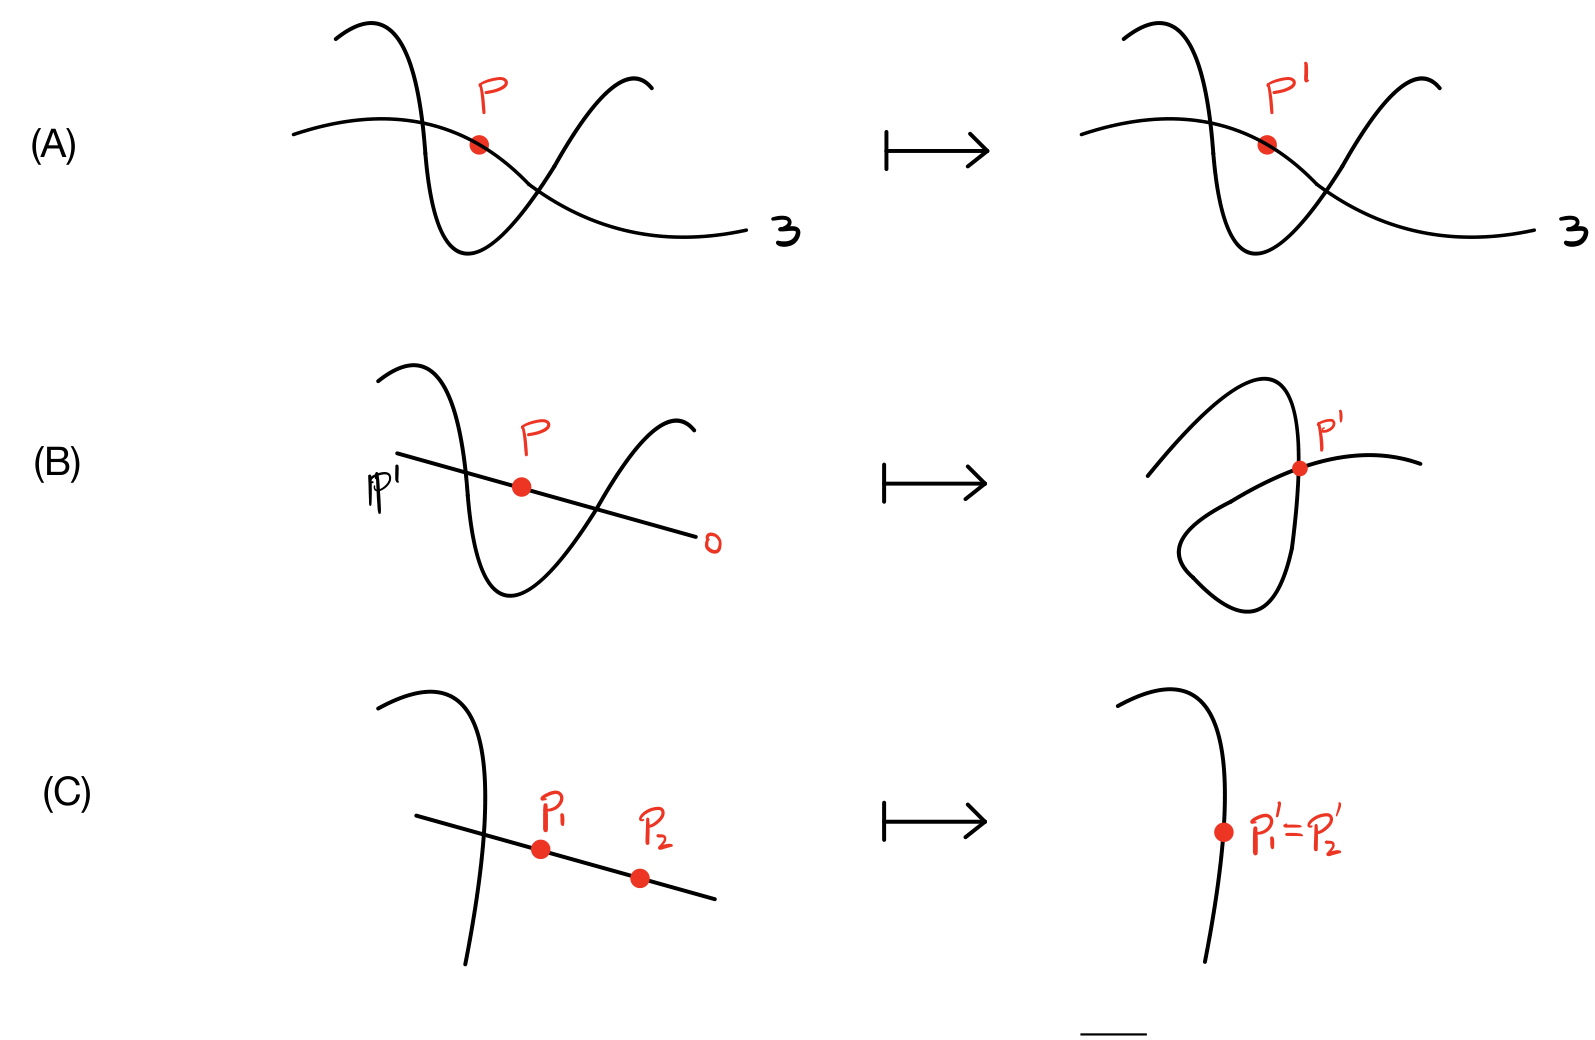
\includegraphics[width=.65\textwidth]{figures/fig-6.6.11.png}
\caption{映射 $\overline{\mathcal M}_{g,\allowbreak n}\to\mathcal U_{g,\allowbreak n}$ 的例子.}\label{src:6.6.11}\end{figure}
\begin{proposition}\label{src:6.6.12}
态射 $\overline{\mathcal M}_{g,\allowbreak n+1}\to\mathcal U_{g,\allowbreak n}$ 是 $\overline{\mathcal M}_{g,\allowbreak n}$ 上的同构. 换言之, 遗忘态射 $\overline{\mathcal M}_{g,\allowbreak n+1}\to\overline{\mathcal M}_{g,\allowbreak n}$ 是泛族.
\end{proposition}
\begin{proof}
由稳定约化 (\bookref{6.5.1}), 两个叠 $\overline{\mathcal M}_{g,\allowbreak n+1}$ 和 $\mathcal U_{g,\allowbreak n}$ 在 $\overline{\mathcal M}_{g,\allowbreak n}$ 上均固有且可表. 因而 $\overline{\mathcal M}_{g,\allowbreak n+1}\to\mathcal U_{g,\allowbreak n}$ 固有且可表. 对每个代数闭域 $k$, 同构类上的诱导映射 $\overline{\mathcal M}_{g,\allowbreak n+1}(k)/{\sim}\to\mathcal U_{g,\allowbreak n}(k)/{\sim}$ 是双射. 故该态射固有拟有限, 因而有限. 另一方面, 它在参数化 $(C,\allowbreak p_1,\allowbreak \ldots,\allowbreak p_n)$ 不含有理桥的带标记曲线 $(C,\allowbreak p_1,\allowbreak \ldots,\allowbreak p_{n+1})$ 的开子叠, 与参数化 $p_{n+1}\in C$ 为不与 $p_1,\allowbreak \ldots,\allowbreak p_n$ 重合的光滑点的开子叠之间诱导同构, 故双有理. 由定理~\bookref{6.4.16}, $\overline{\mathcal M}_{g,\allowbreak n+1}$ 光滑. 因为 $\mathcal U_{g,\allowbreak n}\to\overline{\mathcal M}_{g,\allowbreak n}$ 的纤维是 Cohen--Macaulay 的, 且基底光滑, $\mathcal U_{g,\allowbreak n}$ 是 Cohen--Macaulay 的. 此叠在 $p_{n+1}\in C$ 为光滑点的开轨迹上正则, 该轨迹的补集的余维为 $2$, 故 Serre 正规性判据保证 $\mathcal U_{g,\allowbreak n}$ 正规. 正规 Deligne--Mumford 叠之间的有限双有理态射必为同构.
\end{proof}
\begin{remark}\label{src:6.6.13}
还可显式构造逆态射 $\mathcal U_{g,\allowbreak n}\to\overline{\mathcal M}_{g,\allowbreak n+1}$. 设 $(\mathcal C\to\allowbreak S,\allowbreak \sigma_i)$ 为 $n$-点稳定曲线族, $\tau:S\to\mathcal C$ 是由理想层 $\mathcal I_\tau$ 定义的额外截面. 由
\[
0\to\mathcal O_{\mathcal C}\xrightarrow{(\alpha,\beta)}\mathcal I_\tau^\vee\oplus\mathcal O_{\mathcal C}(\sigma_1+\cdots+\sigma_n)\to\mathcal K\to0
\]
定义凝聚 $\mathcal O_{\mathcal C}$-模 $\mathcal K$, 其中 $\alpha$ 是包含 $\mathcal I_\tau\hookrightarrow\mathcal O_{\mathcal C}$ 的对偶, $\beta$ 为自然包含. 定义
\[
\widetilde{\mathcal C}=\operatorname{Proj}_S\operatorname{Sym}\mathcal K\to\mathcal C.
\]
经过一些工作可证 $\tau^*(\mathcal I_\tau^\vee/\mathcal O_{\mathcal C})$ 为线丛~\cite[引理 2.2]{Knu83a}. 满射 $\tau^*\mathcal K\to\tau^*(\mathcal K/\mathcal O_{\mathcal C})\cong\tau^*(\mathcal I_\tau^\vee/\mathcal O_{\mathcal C})$ 定义截面 $\widetilde\tau:S\to\widetilde{\mathcal C}$. 单射 $\mathcal I_\tau^\vee\to\mathcal K$ 的余核可认同为 $\mathcal O_{\mathcal C}(\sigma_1+\cdots+\sigma_n)|_{\bigcup_i\sigma_i}$, 满射 $\sigma_i^*\mathcal K\to\sigma_i^*\mathcal O_{\mathcal C}(\sigma_1+\cdots+\sigma_n)$ 定义截面 $\widetilde\sigma_i:S\to\widetilde{\mathcal C}$. 可检验 $(\widetilde{\mathcal C}\to\allowbreak S,\allowbreak \widetilde\sigma_1,\allowbreak \ldots,\allowbreak \widetilde\sigma_n,\allowbreak \widetilde\tau)$ 是 $(n+1)$-点稳定曲线族, $c:\widetilde{\mathcal C}\to\mathcal C$ 是 $n$-点预稳定族 $(\widetilde{\mathcal C},\allowbreak \widetilde\sigma_1,\allowbreak \ldots,\allowbreak \widetilde\sigma_n)$ 的稳定收缩, 且 $\sigma_i=c\circ\widetilde\sigma_i$, $\tau=c\circ\widetilde\tau$. 许多情形中, $\widetilde{\mathcal C}\to\mathcal C$ 可更直接地构造为爆破: 例如, 若 $\mathcal C\to\allowbreak S$ 是离散赋值环谱上的一般光滑稳定曲线族, $\mathcal C$ 正则, $\tau:S\to\mathcal C$ 为截面且 $\tau(0)\in\mathcal C_0$ 是结点, 则 $\widetilde{\mathcal C}\to\mathcal C$ 就是在 $\tau(0)$ 处的爆破, $\widetilde\tau$ 是 $\tau$ 的严格变换. 见~\cite[定理 2.4]{Knu83a} 和~\cite[\S X.8]{ACG11}.
\end{remark}
\subsection{粘合态射}\label{src:6.6.3-subsection}
证明曲线族的截面可粘为结点族 (命题~\bookref{6.6.15}) 后, 我们说明存在良定义的有限态射 $\overline{\mathcal M}_{i,\allowbreak k}\times\overline{\mathcal M}_{g-i,\allowbreak n-k+2}\to\overline{\mathcal M}_{g,\allowbreak n}$ 和 $\overline{\mathcal M}_{g-1,\allowbreak n+2}\to\overline{\mathcal M}_{g,\allowbreak n}$ (推论~\bookref{6.6.16}), 称为\newterm{粘合态射}{gluing morphism} (有时也称 clutching morphism).
\begin{figure}[H]\centering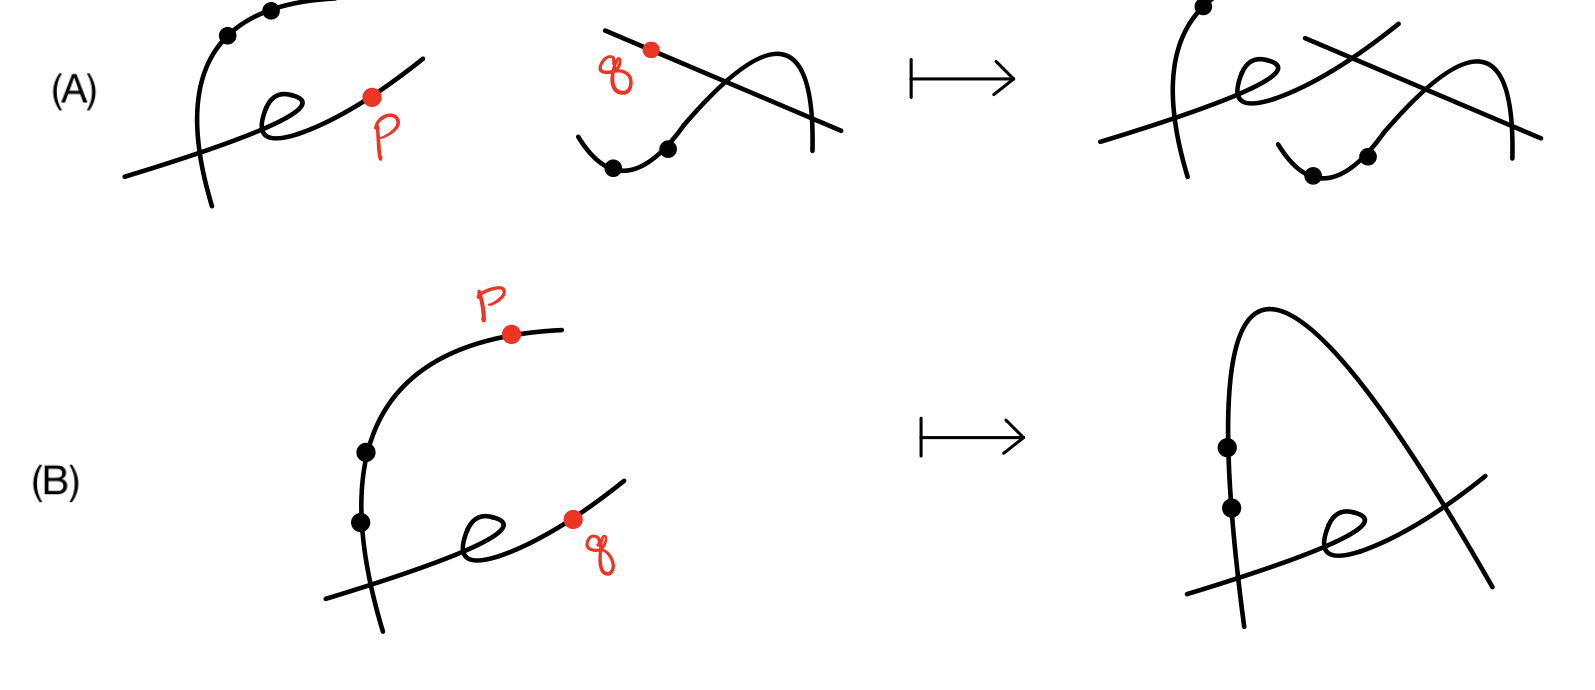
\includegraphics[width=.7\textwidth]{figures/fig-6.6.14.png}
\caption{标记点 $p$, $q$ 的结点粘合.}\label{src:6.6.14}\end{figure}
\begin{proposition}[沿截面粘合族]\label{src:6.6.15}
设 $(\mathcal C\to\allowbreak S,\allowbreak \sigma,\allowbreak \tau)$ 是概形 $S$ 上的 $2$-点射影曲线族 (可不连通), 使每个 $s\in S$ 的 $\sigma(s)$, $\tau(s)$ 为 $\mathcal C_s$ 的互异光滑点. 则存在 $S$ 上概形的典范有限态射 $g:\mathcal C\to\mathcal C'$, 使得
\begin{enumerate}[(1)]
\item $\mathcal C'\to\allowbreak S$ 是曲线族, 带截面 $\nu:S\to\mathcal C'$, 满足 $\nu=g\circ\sigma=g\circ\tau$, 且每个 $s\in S$ 的 $\nu(s)\in\mathcal C_s$ 是结点;
\item $g$ 限制为同构 $\mathcal C\setminus(\sigma(S)\cup\tau(S))\xrightarrow{\sim}\mathcal C'\setminus\nu(S)$, 拓扑空间 $|\mathcal C'|$ 可认同为 $|\mathcal C|$ 对等价关系 $\sigma(s)\sim\tau(s)$ ($s\in S$) 的商;
\item $\mathcal C'$ 可认同为 $\sigma\amalg\tau:S\amalg S\to\mathcal C$ 与投影 $S\amalg S\to\allowbreak S$ 的 Ferrand 推出 (\bookref{B.4.1}); 特别地, 对每个开集 $U\subseteq\mathcal C'$,
\[
\Gamma(U,\mathcal C')=\{f\in\Gamma(g^{-1}(U),\mathcal C)\mid\sigma^*f=\tau^*f\};
\]
\item 此构造与基变换 $T\to\allowbreak S$ 相容.
\end{enumerate}
\end{proposition}
\begin{proof}
因为 $\mathcal C\to\allowbreak S$ 射影, 纤维 $\mathcal C_s$ 的任意两点包含在 $\mathcal C$ 的一个仿射开子概形中. 因而 Ferrand 推出 (\bookref{B.4.1})
\[
\begin{tikzcd}
S\amalg S\arrow[r,"\sigma\amalg\tau"]\arrow[d]&\mathcal C\arrow[d]\\
S\arrow[r,"\nu"']\arrow[ur,phantom,"\lrcorner"]&\mathcal C'
\end{tikzcd}
\]
作为概形 $\mathcal C'$ 存在. 由推出的泛性质, 有自然映射 $\mathcal C'\to\allowbreak S$. 因为 $S\amalg S\to\allowbreak S$ 有限, $\mathcal C\to\mathcal C'$ 也有限. 因为 $S\amalg S\to\allowbreak S$ 平坦, 由推出的性质 (\bookref{B.4.8}(4)), 构造与任意基变换相容. 这给出 (2)--(4).

为证 (1), 先注意 $\mathcal C\to\mathcal C'$ 有限, 故 $\mathcal C'\to\allowbreak S$ 固有. 由光滑态射的局部结构 (\bookref{A.3.4}), 对每个 $s\in S$, 存在仿射开邻域 $\Spec A\subseteq S$ 以及 $\sigma(s)$, $\tau(s)$ 的平展邻域 $\mathcal C\to\Spec A[x]$, $\mathcal C\to\Spec A[y]$. 由推出的性质 (\bookref{B.4.8}(3)), $\mathcal C'$ 在 $\nu(s)$ 处有与如下推出同构的平展邻域:
\[
\begin{tikzcd}
\Spec(A\times A)\arrow[r,"0\amalg0"]\arrow[d]&\Spec(A[x]\times A[y])\arrow[d]\\
\Spec A\arrow[r]\arrow[ur,phantom,"\lrcorner"]&\Spec A[x,y]/(xy).
\end{tikzcd}
\]
所以 $\mathcal C'\to\allowbreak S$ 平坦, $\nu(s)\in\mathcal C_s$ 是结点.

若 $\omega_{\mathcal C/S}(\sigma+\tau)$ 相对甚丰沛 (应用于稳定曲线时即如此), 也可用整体 $\operatorname{Proj}$ 构造 $\mathcal C'$. 有良定义的态射 $q_\sigma:\omega_{\mathcal C/S}(\sigma+\tau)\to\mathcal O_{\sigma(S)}$ 和 $q_\tau:\omega_{\mathcal C/S}(\sigma+\tau)\to\mathcal O_{\tau(S)}$. 定义 $\mathcal C':=\operatorname{Proj}_S\bigoplus_{d\geq0}\mathcal A_d$, 其中 $\mathcal A_d$ 为纤维积
\[
\begin{tikzcd}[column sep=small]
\mathcal A_d\arrow[r]\arrow[d]&\mathcal O_S\arrow[d]\\
\pi_*(\omega_{\mathcal C/S}(\sigma+\tau)^{\otimes d})\times\pi_*(\omega_{\mathcal C/S}(\sigma+\tau)^{\otimes d})\arrow[r,"\pi_*(q_\sigma^{\otimes d})\times\pi_*(q_\tau^{\otimes d})"']&\mathcal O_S\times\mathcal O_S,
\end{tikzcd}
\]
$\pi:\mathcal C\to\allowbreak S$ 是结构态射. 基本上用同一论证可验证 $\mathcal C'\to\allowbreak S$ 满足所需性质. 见~\cite[定理 3.4]{Knu83a} 和~\cite[\S X.7]{ACG11}.
\end{proof}
\begin{corollary}[粘合态射]\label{src:6.6.16}
假设 $2g-2+n>0$.
\begin{enumerate}[(1)]
\item 若 $2g_1-2+n_1>0$, 置 $g_2=g-g_1$, $n_2=n-n_1+2$, 则存在代数叠的有限态射
\[
\begin{aligned}
\overline{\mathcal M}_{g_1,n_1}\times\overline{\mathcal M}_{g_2,n_2}&\to\overline{\mathcal M}_{g,n},\\
((C,p_i),(D,q_i))&\mapsto(C\amalg_{p_{n_1}\sim q_{n_2}}D,p_1,\ldots,p_{n_1-1},q_1,\ldots,q_{n_2-1}).
\end{aligned}
\]
\item 若 $g\geq1$, 则存在代数叠的有限态射
\[
\overline{\mathcal M}_{g-1,n+2}\to\overline{\mathcal M}_{g,n},\qquad
(C,p_i)\mapsto(C/_{p_{n+1}\sim p_{n+2}},p_1,\ldots,p_{n-2}).
\]
\end{enumerate}
\end{corollary}
\begin{proof}
两种情形下, 沿截面粘合族 (\bookref{6.6.15}) 直接给出到 $\mathcal M_{g,\allowbreak n}^{\mathrm{pre}}$ 的代数叠态射. 稳定性可在几何纤维上检验, 只需证结点粘合 $C\amalg_{p_{n_1}\sim q_{n_2}}D$ 和 $C/_{p_{n+1}\sim p_{n+2}}$ 稳定. 由带标记正规化可判定稳定性 (习题~\bookref{6.3.7}), 故这显然成立. 两个映射都是固有 Deligne--Mumford 叠之间的拟有限可表态射, 因而有限.
\end{proof}
更一般地, 对有限指标集 $I$, 可定义亏格 $g$ 的 $I$-点稳定曲线, 记此类曲线的叠为 $\overline{\mathcal M}_{g,\allowbreak I}$. 双射 $I\cong\{1,\allowbreak \ldots,\allowbreak n\}$ 诱导同构 $\overline{\mathcal M}_{g,\allowbreak I}\cong\overline{\mathcal M}_{g,\allowbreak n}$. 推论~\bookref{6.6.16} 自然推广为有限态射
\[
\overline{\mathcal M}_{g_1,I_1}\times\overline{\mathcal M}_{g_2,I_2}\to\overline{\mathcal M}_{g_1+g_2,(I_1\cup I_2)\setminus\{i_1,i_2\}},\qquad
\overline{\mathcal M}_{g-1,J}\to\overline{\mathcal M}_{g,J\setminus\{j_1,j_2\}},
\]
分别粘合标记点 $i_1\in I_1$, $i_2\in I_2$, 或 $j_1,\allowbreak j_2\in J$, 并要求满足各叠非空的数值条件.
\subsection{边界除子}\label{src:6.6.4-subsection}
定义 $\overline{\mathcal M}_{g,\allowbreak n}$ 的边界除子 $\delta_{i,\allowbreak I}$, 并证明总边界除子 $\delta$ 是正规交叉除子 (命题~\bookref{6.6.19}). $\overline{\mathcal M}_{g,\allowbreak n}$ 上的线丛将在~\bookref{6.10} 节讨论.
\begin{definition}[边界除子]\label{src:6.6.17}
设 $2g-2+n>0$. 令 $0\leq i\leq g$ 为整数, $I\subseteq\{1,\allowbreak \ldots,\allowbreak n\}$ 为子集, 满足 $1-2i<|I|<2(g-i)+n-1>0$ (保证 $\overline{\mathcal M}_{i,\allowbreak I\cup\{p\}}$ 与 $\overline{\mathcal M}_{g-i,\allowbreak I^c\cup\{q\}}$ 都非空). \newterm{边界除子}{boundary divisor} 定义为 $\overline{\mathcal M}_{g,\allowbreak n}$ 的闭子叠
\[
\begin{aligned}
\delta_{i,I}&=\operatorname{im}\bigl(\overline{\mathcal M}_{i,I\cup\{p\}}\times\overline{\mathcal M}_{g-i,I^c\cup\{q\}}\to\overline{\mathcal M}_{g,I\cup I^c}\cong\overline{\mathcal M}_{g,n}\bigr),\\
\delta_0&=\operatorname{im}\bigl(\overline{\mathcal M}_{g-1,n+2}\to\overline{\mathcal M}_{g,n}\bigr),\\
\delta&=\delta_0\cup\bigcup_{i,I}\delta_{i,I},
\end{aligned}
\]
约定 $g=0$ 时 $\delta_0$ 为空.
\end{definition}
注意 $\delta_{i,\allowbreak I}=\delta_{g-i,\allowbreak I^c}$. 若 $n=0$, 则 $\delta=\delta_0\cup\cdots\cup\delta_{\lfloor g/2\rfloor}$. 若 $g=0$, 则 $\delta$ 是大小 $2\leq|I|\leq n-2$ 的子集 $I$ 对应的 $\delta_I$ 的并.
\begin{figure}[H]\centering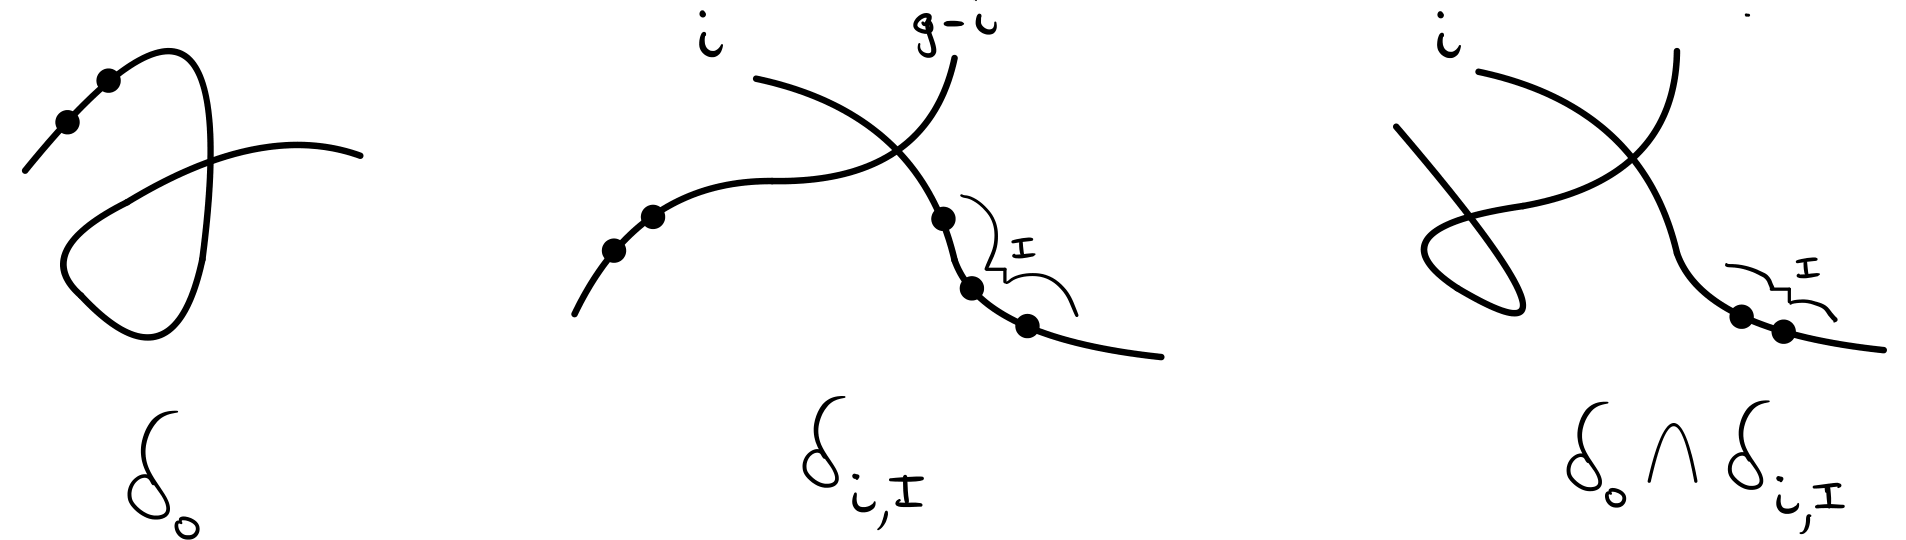
\includegraphics[width=.85\textwidth]{figures/fig-6.6.18.png}
\caption{边界中的稳定曲线的例子.}\label{src:6.6.18}\end{figure}
Deligne--Mumford 叠的闭子叠 $\mathcal Z\subseteq\mathcal X$ 称为有效 Cartier 除子 (分别地, 正规交叉除子), 若有平展展现 $U\to\mathcal X$, 使 $\mathcal Z\times_{\mathcal X}U\subseteq U$ 是有效 Cartier 除子 (分别地, 正规交叉除子). 回顾正则概形的有效 Cartier 除子 $U\subseteq X$ 具有正规交叉, 是指对每个 $u\in U$,
\[
\widehat{\mathcal O}_{U,u}\cong\widehat{\mathcal O}_{X,x}/(f_1\cdots f_k),
\]
其中 $f_1,\allowbreak \ldots,\allowbreak f_k\in\widehat{\mathcal O}_{X,\allowbreak x}$ 可延拓为正则参数系 $f_1,\allowbreak \ldots,\allowbreak f_n$.
\begin{proposition}\label{src:6.6.19}
在域 $k$ 上, $\delta\subseteq\overline{\mathcal M}_{g,\allowbreak n}$ 是正规交叉除子.
\end{proposition}
\begin{proof}
简单的维数计算表明 $\delta$ 纯维, 维数为 $3g-2+n$. 为证正规交叉, 可假设 $k$ 代数闭. 设 $(C,\allowbreak p_i)\in\overline{\mathcal M}_{g,\allowbreak n}$ 是结点为 $q_1,\allowbreak \ldots,\allowbreak q_s\in C$ 的稳定曲线, $(U,\allowbreak u)\to(\overline{\mathcal M}_{g,\allowbreak n},\allowbreak [C,\allowbreak p_i])$ 是平展邻域, $U$ 为概形. 由从局部到整体的形变正合列 (\bookref{6.3.28}), 有一阶形变空间的满射
\begin{equation}\label{src:6.6.20}
\operatorname{Def}(C,p_i)\to\bigoplus_j\operatorname{Def}(\widehat{\mathcal O}_{C,q_j}),
\end{equation}
其中 $\operatorname{Def}(\widehat{\mathcal O}_{C,\allowbreak q_j})\cong k$.

令 $\operatorname{Art}_k$ 为剩余域为 $k$ 的局部 Artin $k$-代数范畴. 定义函子 $F,\allowbreak G_j:\operatorname{Art}_k\to\Sets$: $F(A)$ 为 $(\mathcal C\to\Spec A,\allowbreak \sigma_i,\allowbreak \alpha)$ 的同构类集合, 其中 $(\mathcal C\to\Spec A,\allowbreak \sigma_i)$ 是 $n$-点稳定曲线族, $\alpha:(C,\allowbreak p_i)\xrightarrow{\sim}(\mathcal C\times_A k,\allowbreak \sigma_i\times_A k)$ 为同构; $G_j(A)$ 为 $(B,\allowbreak \beta)$ 的同构类集合, 其中 $B$ 是平坦 $A$-代数, $\beta:\widehat{\mathcal O}_{C,\allowbreak q_j}\xrightarrow{\sim}B\otimes_A A/\mathfrak m_A$ 为同构. 映射 $\Spec\widehat{\mathcal O}_{U,\allowbreak u}\to\overline{\mathcal M}_{g,\allowbreak n}$ 诱导 $F$ 在 $k[[x_1,\allowbreak \ldots,\allowbreak x_{3g-3+n}]]$ 上的极小泛形式形变. 由 Rim--Schlessinger 判据 (\bookref{C.4.6}), $G_j$ 在 $k[[z_j]]$ 上有极小泛形式形变 (见习题~\bookref{C.4.16}). 因为~\bookeqref{6.6.20} 满射, 函子的自然态射 $F\to\bigoplus_jG_j$ 是泛的 (或形式光滑的), 换言之, 自然映射
\begin{equation}\label{src:6.6.21}
\widehat{\mathcal O}_{U,u}\cong k[[x_1,\ldots,x_{3g-3+n}]]\to k[[z_1,\ldots,z_s]]
\end{equation}
满射. 因而可写 $\widehat{\mathcal O}_{U,\allowbreak u}\cong k[[z_1,\allowbreak \ldots,\allowbreak z_s,\allowbreak x'_{s+1},\allowbreak \ldots,\allowbreak x'_{3g-3+n}]]$, 使~\bookeqref{6.6.21} 将每个 $z_i$ 映为自身. 置 $\delta_U=\delta\times_{\overline{\mathcal M}_{g,\allowbreak n}}U$, 得到 $\widehat{\mathcal O}_{\delta_U,\allowbreak u}\cong\widehat{\mathcal O}_{U,\allowbreak u}/(z_1\cdots z_s)$. 另见~\cite[定理 5.2]{DM69}, 其中更一般地证明了 $\delta$ 是 $\mathbb Z$ 上的相对正规交叉除子.
\end{proof}
\begin{exercise}\label{src:6.6.22}
证明 $\overline{\mathcal M}_{0,\allowbreak n}$ 有 $2^{n-1}-n-1$ 个不可约边界除子.
\end{exercise}
\begin{exercise}\label{src:6.6.23}
稳定曲线 $C$ 的对偶图 $\Gamma=(G,\allowbreak w,\allowbreak m)$ 定义于定义~\bookref{6.3.9}.
\begin{enumerate}[(a)]
\item 证明每个对偶图 $\Gamma$ 对应一个局部闭子叠 $\mathcal M_\Gamma\subseteq\overline{\mathcal M}_{g,\allowbreak n}$, 参数化对偶图为 $\Gamma$ 的稳定曲线, 从而有分层
\[
\overline{\mathcal M}_{g,n}=\coprod_\Gamma\mathcal M_\Gamma,
\]
称为\newterm{对偶图分层}{dual graph stratification}.
\item 给定两个对偶图 $\Gamma$, $\Gamma'$, 给出 $\mathcal M_{\Gamma'}\subseteq\overline{\mathcal M_\Gamma}$ 的组合条件.
\item $\overline{\mathcal M}_2$ 的对偶图分层见图~\bookref{6.3.10-figure}. 描述 $\overline{\mathcal M}_{2,\allowbreak 1}$ 和 $\overline{\mathcal M}_3$ 的分层.
\end{enumerate}
\end{exercise}

% Source printed pp. 264-278 / PDF pp. 272-286.
\section{不可约性}\label{src:6.7}
\begin{epigraph}
你在``附录''中提到 Matsusaka 的一个结果, 即任意特征下亏格 $g$ 曲线的模簇的连通性或不可约性, 我此前并未听说. 我不知道这有代数证明 (无论如何表述). 不过, 我有些希望利用特征 $0$ 下的超越结果和连通性定理, 证明 $M_{g,\allowbreak n}$ (任意水平) 的连通性; 但首先应得到 $M_{g,\allowbreak n}$ 的自然``紧化'', 它在 $\mathbb Z$ 上应是单纯的\footnote{Grothendieck 最初称光滑态射为单纯态射.}.
\epigraphauthor{Alexander Grothendieck, 致 Mumford 的信, 1961 年~\cite[638 页]{Mum10}}
\end{epigraph}
我们给出 $\overline{\mathcal M}_{g,\allowbreak n}$ 不可约的若干论证:
\begin{itemize}
\item Clebsch, Lüroth 和 Hurwitz 的经典拓扑论证 (定理~\bookref{6.7.19});
\item 特征 $0$ 下利用光滑曲线的退化和边界 $\delta=\overline{\mathcal M}_g\setminus\mathcal M_g$ 的归纳结构的纯代数论证 (定理~\bookref{6.7.30});
\item 归结到特征 $0$ 的特征 $p>0$ 下的证明 (定理~\bookref{6.7.33}).
\end{itemize}
这些证明从根本上依赖~\bookref{6.7.1-subsection} 节讨论的分歧覆盖理论.

\noindent\textbf{等价性.} 先说明 $\overline{\mathcal M}_{g,\allowbreak n}$, $\mathcal M_g$ 及其粗模空间的连通性与不可约性之间的关系. 因为 $\overline{\mathcal M}_{g,\allowbreak n}$ 是域 $k$ 上的光滑代数叠, 不可约性等价于连通性. 此外, $\overline{\mathcal M}_{g,\allowbreak n+1}\to\overline{\mathcal M}_{g,\allowbreak n}$ 是泛族 (命题~\bookref{6.6.12}), 纤维连通, 因而只需检验 $\overline{\mathcal M}_g$ 连通. 有等价关系
\[
\begin{aligned}
\overline{\mathcal M}_{g,n}\text{ 在 }k\text{ 上不可约}
&\iff\overline{\mathcal M}_{g,n}\text{ 在 }k\text{ 上连通}\\
&\iff\overline{\mathcal M}_g\text{ 在 }k\text{ 上连通}\\
&\iff\mathcal M_g\text{ 在 }k\text{ 上连通且在 }\overline{\mathcal M}_g\text{ 中稠密}.
\end{aligned}
\]
最后, 粗模空间 $\overline{\mathcal M}_{g,\allowbreak n}\to\overline M_{g,\allowbreak n}$ 诱导拓扑空间的同胚 $|\overline{\mathcal M}_{g,\allowbreak n}|\xrightarrow{\sim}|\overline M_{g,\allowbreak n}|$, 故各陈述均可用粗模空间表述.
\subsection{分歧覆盖}\label{src:6.7.1-subsection}
设 $f:C\to\allowbreak D$ 是代数闭域 $k$ 上光滑, 连通射影曲线的有限态射. 假设 $f$ 可分, 即函数域的诱导映射 $K(D)\to\allowbreak K(C)$ 为可分扩张. 对像为 $q\in D(k)$ 的点 $p\in C(k)$, \newterm{分歧指数}{ramification index} $e_p$ 是使映射 $\mathcal O_{D,\allowbreak q}\to\mathcal O_{C,\allowbreak p}$ 满足 $s\mapsto ut^{e_p}$ 的整数, 其中 $s,\allowbreak t$ 是一致化参数, $u$ 为单位. 称 $f$
\[
\begin{cases}
\text{在 }p\text{ 处分歧},&e_p>1;\\
\text{在 }p\text{ 处温和分歧},&e_p>1,\ \operatorname{char}(k)=0\text{ 或 }\operatorname{char}(k)\nmid e_p;\\
\text{在 }p\text{ 处非分歧},&e_p=1.
\end{cases}
\]
若 $f$ 在 $p$ 处非分歧, 则 $f(p)$ 上方的概形论纤维在 $p$ 处同构于 $\Spec\kappa(p)$, 故与非分歧的通常定义一致 (定理~\bookref{A.3.3}). 此外, 因为 $f$ 平坦, 在 $p$ 处非分歧当且仅当在 $p$ 处平展.

有微分的短正合列
\begin{equation}\label{src:6.7.1}
0\to f^*\Omega_D\to\Omega_C\to\Omega_{C/D}\to0.
\end{equation}
此列总是右正合. 因为 $f^*\Omega_D$, $\Omega_C$ 是线丛, 左方映射单射当且仅当非零. 由于 $K(D)\to\allowbreak K(C)$ 可分, $\Omega_{C/D}\otimes K(C)=\Omega_{K(C)/K(D)}=0$, 因而 $f^*\Omega_D\to\Omega_C$ 在一般点处非零. 在点 $p\in C(k)$ 的茎上考察此列, 微分 $dt$ 映为 $d(us^{e_p})=e_pus^{e_p-1}ds+s^{e_p}du$. 若 $f$ 在 $p$ 处温和分歧, 则 $(\Omega_{C/D})_p\cong\mathcal O_{C,\allowbreak p}(ds)/(s^{e_p-1}ds)$, 且 $\operatorname{length}(\Omega_{C/D})_p=\dim\Omega_{C/D}\otimes\kappa(p)=e_p-1$.
\begin{definition}\label{src:6.7.2}
设 $k$ 为代数闭域.
\begin{enumerate}[(1)]
\item \newterm{分歧覆盖}{branched covering} 是 $k$ 上光滑, 连通射影曲线的有限可分态射 $f:C\to\allowbreak D$.
\item \newterm{单分歧覆盖}{simply branched covering} 是每个纤维至多含一个分歧点, 且每个分歧点 $p\in C(k)$ 均温和分歧, 分歧指数 $e_p=2$ 的分歧覆盖.
\end{enumerate}
\end{definition}
\begin{figure}[H]\centering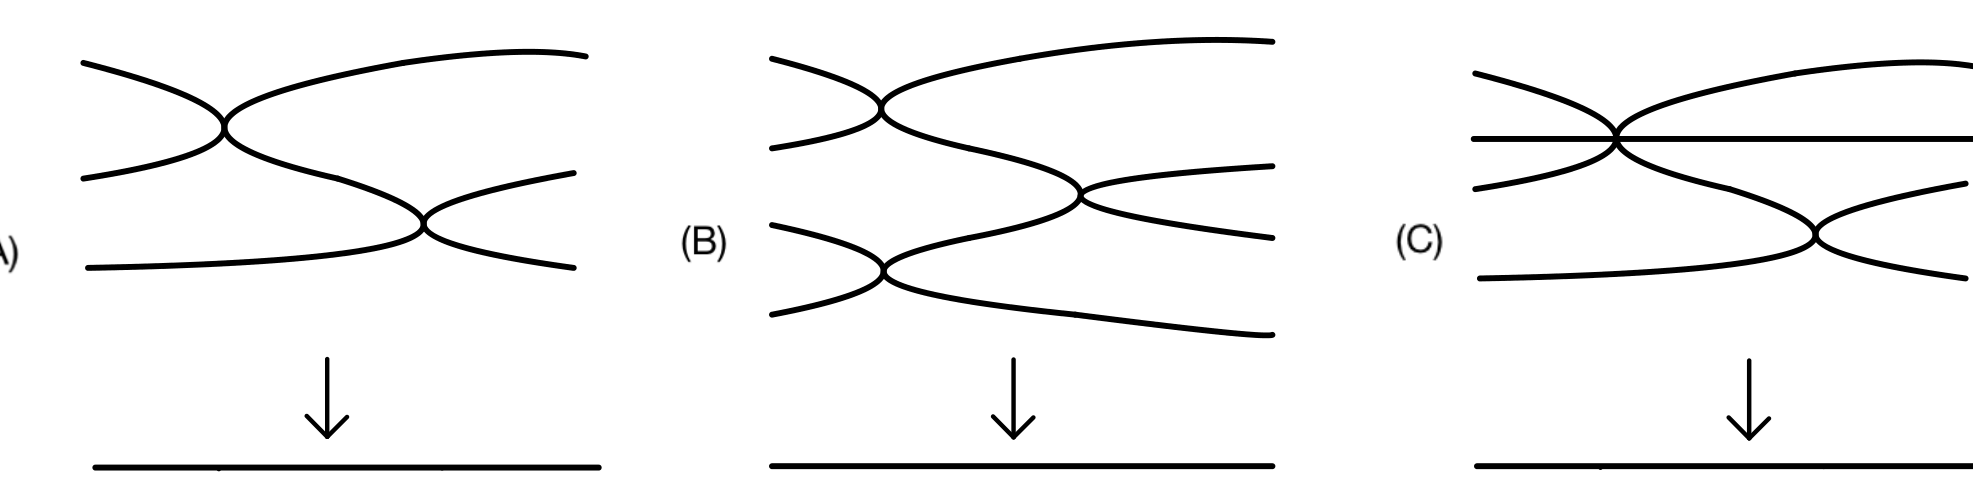
\includegraphics[width=.85\textwidth]{figures/fig-6.7.3.png}
\caption{$\mathbb P^1$ 上分歧覆盖的例子: (A) 单分歧, (B), (C) 则不是. 虽然图中源曲线 $C$ 看起来不光滑, 它在基域 $k$ 上实际上光滑. 但映射 $C\to\mathbb P^1$ 不光滑, 图示旨在反映 $C$ 在 $\mathbb P^1$ 上的奇点.}\label{src:6.7.3}\end{figure}
若 $f:C\to\allowbreak D$ 是分歧覆盖, \newterm{分歧除子}{ramification divisor} 定义为
\[
R=\sum_{p\in C(k)}\operatorname{length}(\Omega_{C/D})_p\cdot p
\overset{\text{若 }f\text{ 温和分歧}}{=}\sum_{p\in C(k)}(e_p-1).
\]
\begin{theorem}[Riemann--Hurwitz]\label{src:6.7.4}
若 $f:C\to\allowbreak D$ 是分歧除子为 $R$ 的分歧覆盖, 则 $\Omega_C\cong f^*\Omega_D\otimes\mathcal O_C(R)$, 且
\[
2g(C)-2=\deg(f)(2g(D)-2)+\deg R.
\]
特别地, 若 $f:C\to\mathbb P^1$ 单分歧, 则它在 $2g+2d-2$ 个互异点上方分歧.
\end{theorem}
\begin{proof}
直接由正合列~\bookeqref{6.7.1} 得出. 另见~\cite[命题 IV.2.3]{Har77}.
\end{proof}
\begin{example}\label{src:6.7.5}
分歧覆盖的局部模型为 $x\mapsto x^n$ 定义的 $f:\mathbb A^1\to\mathbb A^1$. 相对微分层为 $\Omega_{\mathbb A^1/\mathbb A^1}=k[x]\langle dx\rangle/(nx^{n-1}dx)$. 因而若 $\operatorname{char}(k)\nmid n$, $f$ 是在 $\mathbb A^1\setminus0$ 上平展, 在 $0$ 处以指数 $n-1$ 温和分歧的分歧覆盖.
\end{example}
\begin{exercise}\label{src:6.7.6}
证明每个分歧覆盖在指数 $n-1$ 的分歧点附近, 平展局部同构于 $\mathbb A^1\to\mathbb A^1$, $x\mapsto x^n$.
\end{exercise}
\noindent\textbf{代数, 全纯与拓扑分歧覆盖.} $\mathbb P^1$ 的全纯 (分别地, 拓扑) 分歧覆盖是非恒定全纯 (分别地, 连续) 态射 $f:C\to\mathbb P^1$, 其中 $C$ 是连通紧 Riemann 曲面 (分别地, 连通 Hausdorff 紧拓扑空间, 且 $f$ 在 $\mathbb P^1$ 的有限个点的补集上是覆盖空间).
\begin{proposition}\label{src:6.7.7}
在 $\mathbb C$ 上有自然双射
\[
\{C\to\mathbb P^1\text{ 的代数分歧覆盖}\}
\longleftrightarrow\{C\to\mathbb P^1\text{ 的全纯分歧覆盖}\}
\longleftrightarrow\{C\to\mathbb P^1\text{ 的拓扑分歧覆盖}\}.
\]
\end{proposition}
\begin{proof}
代数分歧覆盖全纯, 全纯分歧覆盖是拓扑分歧覆盖. 反之, 若 $f:C\to\mathbb P^1$ 是拓扑覆盖, 则 $\mathbb P^1$ 的全纯结构自然诱导 $C$ 的全纯结构, 使 $f$ 解析. 依赖隐函数定理的经典事实表明, 存在 $C$ 和 $\mathbb P^1$ 的局部坐标片, 使 $f$ 描述为 $z\mapsto z^k$ (参见~\cite[命题 II.4.1]{Mir95}), 这蕴涵 $C$ 代数.
\end{proof}
\noindent\textbf{单值作用.} 设 $f:C\to\mathbb P^1$ 是 $\mathbb C$ 上的 $d$ 次 (拓扑) 分歧覆盖, $B\subseteq\mathbb P^1$ 为分歧轨迹, 即使 $f^{-1}(\mathbb P^1\setminus B)\to\mathbb P^1\setminus B$ 成为覆盖空间的最小点集. 选取基点 $q\in\mathbb P^1\setminus B$. $\pi_1(\mathbb P^1\setminus B,\allowbreak q)$ 在纤维 $f^{-1}(q)$ 上的\newterm{单值作用}{monodromy action} 如下定义: 对 $\gamma\in\pi_1(\mathbb P^1\setminus B,\allowbreak q)$ 和 $p\in f^{-1}(q)$, 路径 $\gamma:[0,\allowbreak 1]\to\mathbb P^1$ 唯一提升为路径 $\widetilde\gamma:[0,\allowbreak 1]\to\allowbreak C$, 满足 $\widetilde\gamma(0)=p$, 并定义 $\gamma\cdot p=\widetilde\gamma(1)$.
\begin{figure}[H]\centering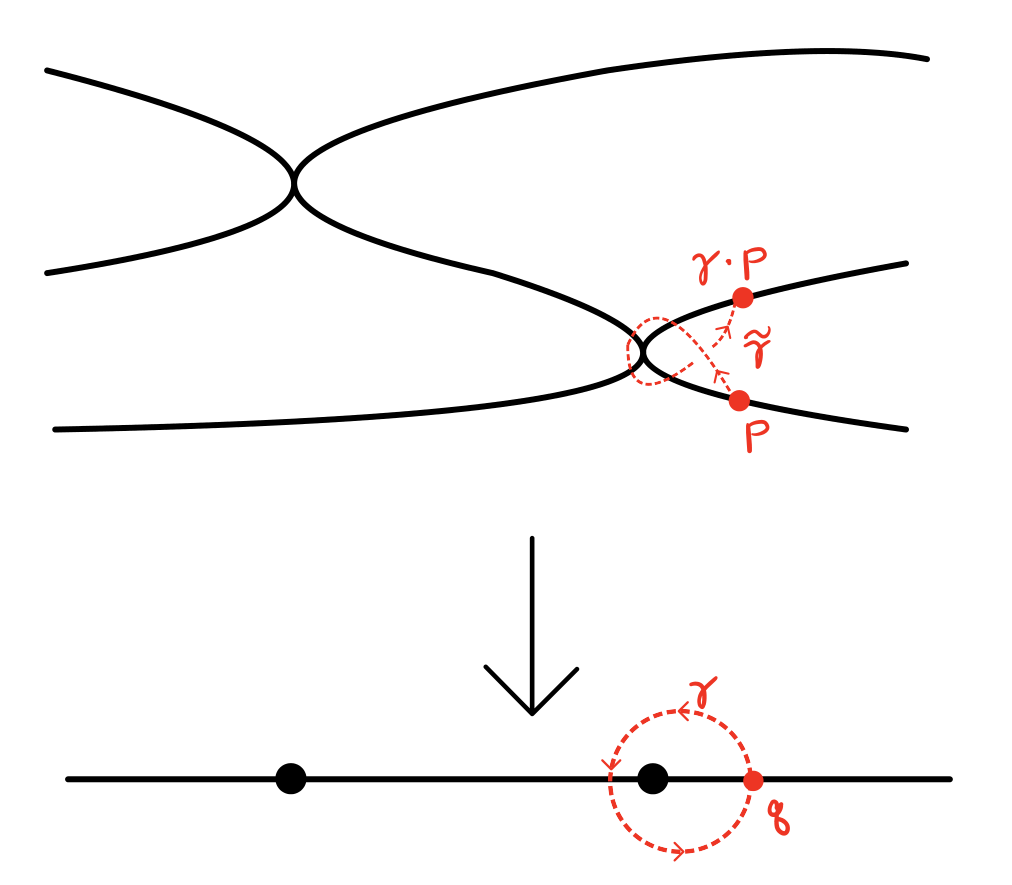
\includegraphics[width=.55\textwidth]{figures/fig-6.7.8.png}
\caption{单值作用.}\label{src:6.7.8}\end{figure}
选择双射 $f^{-1}(p)\cong\{1,\allowbreak \ldots,\allowbreak d\}$ 定义群同态 $\rho:\pi_1(\mathbb P^1\setminus B,\allowbreak q)\to\allowbreak S_d$, 称为\newterm{单值表示}{monodromy representation}. 反之, 每个这样的群同态均由分歧覆盖诱导.
\newpage
\begin{proposition}\label{src:6.7.9}
设 $B\subseteq\mathbb P^1$ 是大小 $b$ 的有限集, $q\in\mathbb P^1\setminus B$, $d>0$ 为正整数. 基本群 $\pi_1(\mathbb P^1\setminus B,\allowbreak q)$ 可认同为绕 $B$ 中各点的简单环路 $\sigma_i$ ($i=1,\allowbreak \ldots,\allowbreak b$) 生成的自由群. 有同构类的自然双射
\[
\left\{\begin{array}{l}\text{在 }B\text{ 上方单分歧的}\\d\text{ 次覆盖 }C\to\mathbb P^1\end{array}\right\}/{\sim}
\longleftrightarrow
\left\{\begin{array}{l}\rho:\pi_1(\mathbb P^1\setminus B,q)\to S_d\text{ 为群同态},\\\operatorname{im}(\rho)\subseteq S_d\text{ 是传递子群},\\\text{每个 }\rho(\sigma_i)\text{ 为对换}\end{array}\right\}/{\sim}.
\]
两个覆盖等价指它们在 $\mathbb P^1$ 上同构; 两个同态 $\rho$, $\rho'$ 等价指相差 $S_d$ 的内自同构, 即存在 $h\in S_d$ 使 $\rho'=h^{-1}\rho h$.
\end{proposition}
\begin{proof}
左到右的自然映射已说明. 反之, 给定群同态 $\rho$, 令 $H\subseteq\pi_1(\mathbb P^1\setminus B,\allowbreak q)$ 为固定 $1$ 的元素 $\gamma$ 组成的子群. 它的指数为 $d$, 因而对应于覆盖空间 $C^*\to\mathbb P^1\setminus B$, 可证其延拓为 $d$ 次有限态射 $C\to\mathbb P^1$. $C$ 连通等价于 $\operatorname{im}(\rho)$ 传递, 覆盖单分歧等价于每个 $\rho(\sigma_i)$ 为对换. 见~\cite[命题 III.4.9]{Mir95}.
\end{proof}
\subsection{Hurwitz 模空间}\label{src:6.7.2-subsection}
对正整数 $g,\allowbreak b$, 定义并研究 Hurwitz 模空间
\[
\operatorname{Hur}_{g,b}:=\{\text{在 }b\text{ 个有序点上方单分歧的亏格 }g\text{ 覆盖 }C\to\mathbb P^1\}
\]
及其与 $\mathcal M_g$ 的关系. 由 Riemann--Hurwitz (\bookref{6.7.4}), 若覆盖的次数为 $d$, 则 $b=2g+2d-2$. 文献中 Hurwitz 空间有时记作 $\operatorname{Hur}_{d,\allowbreak b}$ 或 $\operatorname{Hur}_{d,\allowbreak g}$. 关键图为
\begin{equation}\label{src:6.7.10}
\begin{tikzcd}
&\operatorname{Hur}_{g,b}\arrow[dl]\arrow[dr]&\\
\mathcal M_g&&M_{0,b},
\end{tikzcd}
\end{equation}
将单分歧覆盖映到 $C\in\mathcal M_g$ 及 $M_{0,\allowbreak b}$ 中的 $b$ 个有序分歧点.

解析地, $\mathbb C$ 上的 $\operatorname{Hur}_{g,\allowbreak b}$ 可看作使 $\operatorname{Hur}_{g,\allowbreak b}\to\allowbreak M_{0,\allowbreak b}$ 连续的最粗拓扑所赋的拓扑空间. 代数地, 仍采用函子方法定义. 概形 $S$ 上亏格 $g$, 在 $b$ 个有序点上方单分歧的 $\mathbb P^1$ 覆盖族 $(\mathcal C\to\mathcal D\to\allowbreak S,\allowbreak \sigma_i)$, 是光滑亏格 $g$ 曲线族 $\mathcal C\to\allowbreak S$ 和 $b$-点光滑亏格 $0$ 曲线族 $(\mathcal D\to\allowbreak S,\allowbreak \sigma_i)$, 配备 $S$ 上概形的 $d$ 次有限平坦态射 $\mathcal C\to\mathcal D$, 使每个几何点 $s\in S(k)$ 的 $\mathcal C_s\to\mathcal D_s\cong\mathbb P^1_k$ 在 $\sigma_1(s),\allowbreak \ldots,\allowbreak \sigma_b(s)$ 上方单分歧.
\begin{definition}[Hurwitz 函子]\label{src:6.7.11}
对正整数 $g,\allowbreak d$, 置 $b=2g+2d-2$. \newterm{Hurwitz 函子}{Hurwitz functor} 为
\[
\begin{aligned}
\operatorname{Hur}_{g,b}:\Sch&\to\Sets,\\
S&\mapsto\{\text{亏格 }g,\text{ 次数 }d\text{ 的 }\mathbb P^1\text{ 单分歧覆盖族 }(\mathcal C\to\mathcal D\to S,\sigma_i)\}/{\sim},
\end{aligned}
\]
其中两个族等价指存在同构 $\mathcal C\xrightarrow{\sim}\mathcal C'$ 和 $\mathcal D'\xrightarrow{\sim}\mathcal D'$, 与截面和结构态射 $\mathcal C\to\mathcal D$, $\mathcal C'\to\mathcal D'$ 相容.
\end{definition}
有叠的态射 $\operatorname{Hur}_{g,\allowbreak b}\to\mathcal M_g$ 和 $\operatorname{Hur}_{g,\allowbreak b}\to\allowbreak M_{0,\allowbreak b}$, 分别取覆盖族的 $\mathcal C\to\allowbreak S$ 和 $(\mathcal D\to\allowbreak S,\allowbreak \sigma_i)$, 给出图~\bookeqref{6.7.10}.
\begin{remark}[变体]\label{src:6.7.12}
文献中也将上述定义的若干变体称为 Hurwitz 模空间. 首先可刚化模问题, 考虑函子 $\operatorname{Hur}_{g,\allowbreak b}^{\mathrm{rig}}:\Sch\to\allowbreak S$, 在 $S$ 上的对象是从光滑亏格 $g$ 曲线族出发的 $S$ 上有限平坦态射 $\mathcal C\to\mathbb P^1_S$, 配备互不相交的有序截面 $\sigma_1,\allowbreak \ldots,\allowbreak \sigma_b:S\to\mathbb P^1_S$, 使每个几何纤维在这些截面所给点上方单分歧. 两个族等价指它们在 $\mathbb P^1_S$ 上同构且截面相等. 有态射 $\operatorname{Hur}_{g,\allowbreak b}^{\mathrm{rig}}\to(\mathbb P^1)^b\setminus\Delta$, 其中 $\Delta$ 是所有两两对角线的并. 代数群 $\operatorname{PGL}_2$ 自由作用于 $\operatorname{Hur}_{g,\allowbreak b}^{\mathrm{rig}}$, 商可认同为 $\operatorname{Hur}_{g,\allowbreak b}$, 等变态射 $\operatorname{Hur}_{g,\allowbreak b}^{\mathrm{rig}}\to(\mathbb P^1)^b\setminus\Delta$ 的商则认同为 $\operatorname{Hur}_{g,\allowbreak b}\to\allowbreak M_{0,\allowbreak b}$.

另一常见变体是将分歧轨迹看作无序点集, 这是 Hurwitz 在~\cite{Hur91} 中最初考虑的版本. 函子 $\operatorname{Hur}_{g,\allowbreak b}^{\mathrm{rig,\allowbreak unord}}:\Sch\to\Sets$ 的 $S$ 上对象是从光滑亏格 $g$ 曲线族出发的有限平坦态射 $f:\mathcal C\to\mathbb P^1_S$, 使每个几何纤维为在 $b$ 个点上方单分歧的覆盖. 断言有到参数化 $b$ 个无序互异点的空间的态射 $\operatorname{Hur}_{g,\allowbreak b}^{\mathrm{rig,\allowbreak unord}}\to\operatorname{Sym}^b\mathbb P^1\setminus\Delta$. 事实上, 由 $f$ 的相对奇点轨迹定义的分歧除子 $R_f\subseteq\mathcal C$ 在 $S$ 上有限平展, 次数为 $b=2g+2d-2$. 两两对角线的补集 $R_f\times_S\cdots\times_S R_f\setminus\Delta$ 是 $S$ 上的主 $S_b$-挠子 (见习题~\bookref{B.1.55}), 到 $\mathbb P^1_S\times_S\cdots\times_S\mathbb P^1_S\setminus\Delta$ 的映射为 $S_b$-等变. 它定义商叠 $[((\mathbb P^1)^b\setminus\Delta)/S_b]$ 的 $S$-值点, 该商叠可认同为概形 $\operatorname{Sym}^b\mathbb P^1\setminus\Delta$. 还有 $\operatorname{Sym}^b\mathbb P^1\setminus\Delta\cong\mathbb P^b\setminus\Delta$, 后一 $\Delta$ 为判别式超曲面. 对称群 $S_b$ 自由作用于 $\operatorname{Hur}_{g,\allowbreak b}^{\mathrm{rig}}$, 商为 $\operatorname{Hur}_{g,\allowbreak b}^{\mathrm{rig,\allowbreak unord}}$; 相应态射的 $S_b$-商可认同为 $\operatorname{Hur}_{g,\allowbreak b}^{\mathrm{rig,\allowbreak unord}}\to\operatorname{Sym}^b\mathbb P^1\setminus\Delta$.
\end{remark}
下列习题保证 $\operatorname{Hur}_{g,\allowbreak b}\to\allowbreak M_{0,\allowbreak b}$ 有限, 平展且满射, 即代数覆盖空间. 在域 $k$ 上工作时, 也用 $\operatorname{Hur}_{g,\allowbreak b}$ 表示基变换 $\operatorname{Hur}_{g,\allowbreak b}\times_{\mathbb Z}k$.
\begin{exercise}\label{src:6.7.13}
设 $k$ 是特征 $0$ 的代数闭域, $g,\allowbreak b,\allowbreak d$ 是正整数, $b=2g+2d-2$, $d>2$.
\begin{enumerate}[(a)]
\item 证明 $\operatorname{Hur}_{g,\allowbreak b}$ 在 $k$ 上的对角线由概形可表.
\item 若 $\mathcal C\to\mathbb P^1_k$ 是 $d$ 次单分歧覆盖, 证明 $\mathcal C$ 在 $\mathbb P^1$ 上的每个自同构平凡. 推出 $d$ 次 $\mathbb P^1$ 单分歧覆盖族的自同构群概形也平凡.

提示: 用光滑曲线固定超过 $2g+2$ 个点的自同构必平凡 (习题~\bookref{6.1.9}).
\item (困难) 证明 $\operatorname{Hur}_{g,\allowbreak b}\to\allowbreak M_{0,\allowbreak b}$ 是有限平展可表态射. 特别地, Hurwitz 函子由概形可表. 另见~\cite[定理 7.2]{Ful69}, 其中更一般地证明了它在 $\Spec\mathbb Z$ 上可表, 且该映射平展 (在特征大于 $d$ 的基底上有限平展).
\item 验证注记~\bookref{6.7.12} 中两个刚化函子也由概形可表.
\end{enumerate}
\end{exercise}
\begin{remark}\label{src:6.7.14}
下一节证明 Clebsch--Hurwitz--Lüroth 定理 (\bookref{6.7.19}) 时, 只需知道 $\operatorname{Hur}_{g,\allowbreak b}\to\allowbreak M_{0,\allowbreak b}$ 是拓扑覆盖空间, 这有初等论证. 参照图~\bookref{6.7.15}, 给定单分歧覆盖 $f:C\to\mathbb P^1$ 和分歧点 $p\in C$, 可在 $f(p)$ 附近取开邻域 $U\subseteq\mathbb P^1$, 使 $f^{-1}(U)\to\allowbreak U$ 同构于 $x\mapsto x^n$ 给出的 $\mathbb C\to\mathbb C$ 的开邻域. 对每个 $q'\in U$, 可构造分歧覆盖 $C'\to\mathbb P^1$, 在 $U$ 外与原覆盖相同, 在 $U$ 上局部同构于 $x\mapsto x^n$, 但以 $q'$ 而非 $f(p)$ 为中心.
\end{remark}
\begin{figure}[H]\centering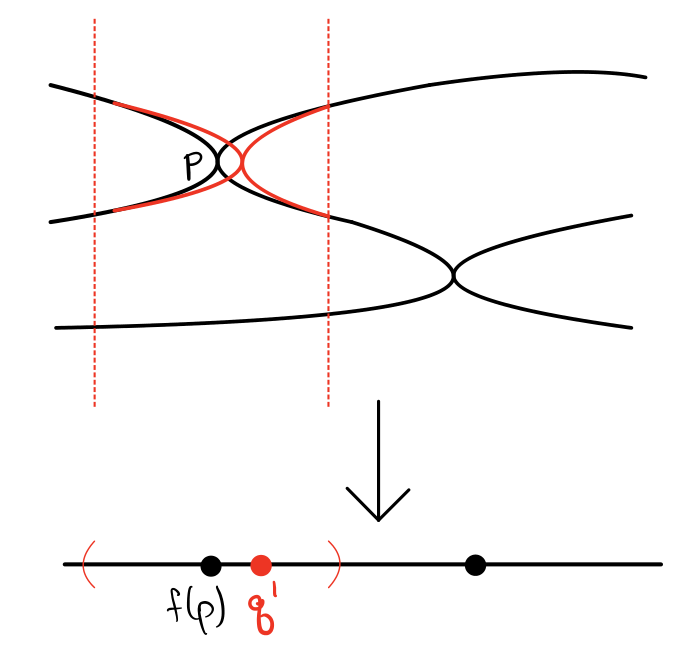
\includegraphics[width=.35\textwidth]{figures/fig-6.7.15.png}
\caption{}\label{src:6.7.15}\end{figure}
现在研究另一映射 $\operatorname{Hur}_{g,\allowbreak b}\to\mathcal M_g$.
\newpage
\begin{lemma}\label{src:6.7.16}
设 $C$ 是特征 $0$ 代数闭域 $k$ 上光滑, 连通, 亏格 $g$ 的射影曲线. 若 $L$ 是次数 $d\geq2g+3$ 的线丛, $V\subseteq\mathrm H^0(C,\allowbreak L)$ 是维数为 $2$ 的线性系, 则选择 $V$ 的基诱导单分歧覆盖 $C\to\mathbb P^1$.
\end{lemma}
\begin{proof}
作维数计算. 因为 $\deg(\omega_C\otimes L^\vee)<0$, 有 $\mathrm h^1(C,\allowbreak L)=\mathrm h^0(C,\allowbreak \omega_C\otimes L^\vee)=0$. Riemann--Roch 给出 $\mathrm h^0(C,\allowbreak L)=d+1-g$, 所以 $2$ 维子空间的 Grassmann 簇 $\operatorname{Gr}(2,\allowbreak \mathrm H^0(L))$ 的维数为 $2(d-g-1)$. 因为 $\operatorname{char}(k)=0$, 每个有限态射 $C\to\mathbb P^1$ 自动可分. 若 $V$ 不诱导单分歧覆盖, 则必满足下列条件之一:
\begin{enumerate}[(a)]
\item $V$ 有基点;
\item 存在分歧指数大于 $2$ 的分歧点;
\item 同一纤维中有两个分歧点.
\end{enumerate}
断言各条件均为余维至少一的闭条件. 对 (a), 若 $p\in C(k)$ 是基点, 则 $V\subseteq\mathrm H^0(C,\allowbreak L(-p))$. 由 $d\geq2g$, 有 $\deg(\omega_C\otimes(L(-p))^\vee)<0$, 因而 $\mathrm h^0(C,\allowbreak L(-p))=d-g$, $\dim\operatorname{Gr}(2,\allowbreak \mathrm H^0(C,\allowbreak L(-p)))=2(d-g-2)$. 让 $p\in C$ 变化, (a) 定义的轨迹维数为 $2(d-g-2)+1=\dim\operatorname{Gr}(2,\allowbreak \mathrm H^0(L))-1$. (b), (c) 留给读者. 另见~\cite{Sev21} 和~\cite[命题 8.1]{Ful69}.
\end{proof}
\begin{exercise}[细节]\label{src:6.7.17}
\begin{enumerate}[(a)]
\item 验证上述 (b), (c) 为余维至少一的闭条件.
\item 证明只要 $\operatorname{char}(k)\ne2$, 论证仍成立, 并说明在特征 $2$ 时为何失效.
\end{enumerate}
\end{exercise}
\begin{corollary}\label{src:6.7.18}
设 $k$ 是特征 $0$ 的代数闭域. 若 $g\geq2$, $d\geq2g+3$, $b=2g+2d-2$, 则态射 $\operatorname{Hur}_{g,\allowbreak b}\to\mathcal M_g$, $(C\to\mathbb P^1,\allowbreak \sigma_i)\mapsto C$ 满射.
\end{corollary}
\subsection{Clebsch--Hurwitz--Lüroth 定理}\label{src:6.7.3-subsection}
给出 Clebsch~\cite{Cle73}, Hurwitz~\cite{Hur91} 和 Lüroth~\cite{Lür71} 证明 $\mathbb C$ 上 Hurwitz 模空间连通的经典论证. 由 $\operatorname{Hur}_{g,\allowbreak b}\to\mathcal M_g$ 满射, 推出 $\mathcal M_g$ 不可约, 这是 Klein~\cite[\S19]{Kle82} 和 Severi~\cite[\S F]{Sev21} 的经典结果. 现代论述见~\cite[命题 1.5]{Ful69}.
\begin{theorem}[Clebsch--Hurwitz--Lüroth 定理]\label{src:6.7.19}
若 $g\geq2$, $d\geq2$, $b=2g+2d-2$, 则 $\mathbb C$ 上的 Hurwitz 模空间 $\operatorname{Hur}_{g,\allowbreak b}$ 连通.
\end{theorem}
\begin{proof}
利用将单分歧覆盖映为有序分歧轨迹的态射 $\beta:\operatorname{Hur}_{g,\allowbreak b}\to\allowbreak M_{0,\allowbreak b}$. 由习题~\bookref{6.7.13}(c), 这是覆盖空间. 对有序互异点集 $B=\{q_1,\allowbreak \ldots,\allowbreak q_b\}\subseteq\mathbb P^1$ 及 $q\in\mathbb P^1\setminus B$, 基本群 $\pi_1(\mathbb P^1\setminus B,\allowbreak q)=\langle\sigma_i\mid\sigma_1\cdots\sigma_b=1\rangle$ 作用于单分歧覆盖 $f:C\to\mathbb P^1$ 的纤维 $f^{-1}(p)$, 其中 $\sigma_i$ 绕 $q_i$ 一周. 同样, 因为 $\beta$ 是覆盖空间, $\pi_1(M_{0,\allowbreak b},\allowbreak B)$ 作用于纤维 $\operatorname{Hur}_{d,\allowbreak B}:=\beta^{-1}(B)\subseteq\operatorname{Hur}_{g,\allowbreak b}$. (注意大写下标 $B$ 与小写 $b$ 的区别.) 由命题~\bookref{6.7.9}, 有双射
\[
\begin{aligned}
\operatorname{Hur}_{g,B}
&=\{\text{在 }B\text{ 上方单分歧的亏格 }g\text{ 覆盖 }C\to\mathbb P^1\}/{\sim}\\
&\cong\left\{\begin{array}{l}\text{群同态 }\rho:\pi_1(\mathbb P^1\setminus B,q)\to S_d,\\\operatorname{im}(\rho)\text{ 传递, 每个 }\rho(\sigma_i)\text{ 为对换}\end{array}\right\}/S_d\text{ 共轭}\\
&\cong\left\{\begin{array}{l}\text{对换序列 }(\tau_1,\ldots,\tau_b)\in(S_d)^b,\\\text{乘积为 }1,\text{ 生成传递子群}\end{array}\right\}/S_d\text{ 共轭}.
\end{aligned}
\]
Hurwitz 空间连通等价于 $\pi_1(M_{0,\allowbreak b},\allowbreak B)$ 在纤维 $\operatorname{Hur}_{d,\allowbreak B}$ 上的作用传递. 考虑序列
\[
\tau=\bigl(\underbrace{(12),(12),(13),(13),\ldots,(1\ d-1),(1\ d-1)}_{2(d-2)},
\underbrace{(1d),(1d),\ldots,(1d)}_{2g+2}\bigr)\in\operatorname{Hur}_{d,B}.
\]
只需证明每个轨道包含 $\tau$. 为此定义环路
\[
\begin{aligned}
\Gamma_i:[0,1]&\to M_{0,b},\\
t&\mapsto(q_1,\ldots,q_{i-1},\gamma_i(t),\gamma'_i(t),q_{i+2},\ldots,q_b),
\end{aligned}
\]
其中 $\gamma_i$, $\gamma'_i$ 如图~\bookref{6.7.20}.
\begin{figure}[H]\centering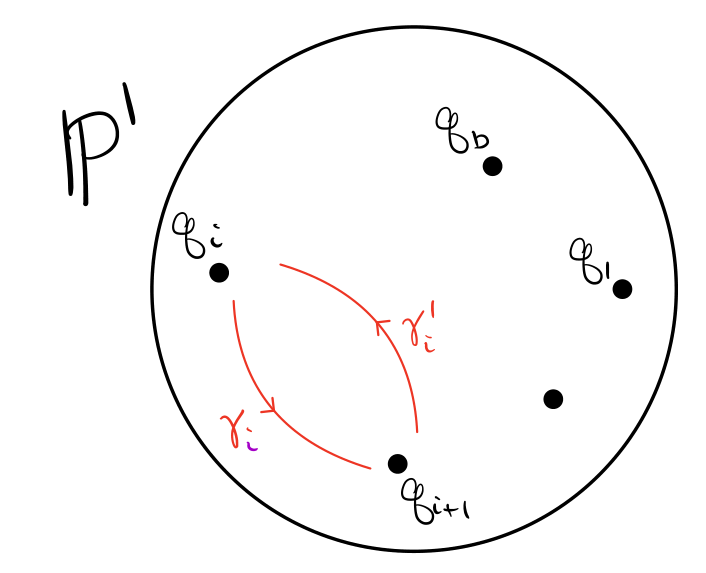
\includegraphics[width=.35\textwidth]{figures/fig-6.7.20.png}
\caption{$\mathbb P^1$ 中的路径.}\label{src:6.7.20}\end{figure}
对 $(\lambda_1,\allowbreak \ldots,\allowbreak \lambda_b)\in\operatorname{Hur}_{g,\allowbreak b}$, $\Gamma_i$ 的作用为
\[
\Gamma_i\cdot(\lambda_1,\ldots,\lambda_b)
=(\lambda_1,\ldots,\lambda_{i-1},\lambda_{i-1}^{-1}\lambda_{i+1}\lambda_i,\lambda_i,\lambda_{i+2},\ldots,\lambda_b).
\]
剩下是组合问题: 证明存在环路序列 $\Gamma_{i_1},\allowbreak \ldots,\allowbreak \Gamma_{i_k}$, 使 $\tau=\Gamma_{i_1}\Gamma_{i_2}\cdots\Gamma_{i_k}\cdot(\lambda_1,\allowbreak \ldots,\allowbreak \lambda_b)$. 留给读者.
\end{proof}
\begin{exercise}\label{src:6.7.21}
解决上述证明末尾的组合问题.
\end{exercise}
\begin{corollary}[$\mathcal M_g$ 的不可约性]\label{src:6.7.22}
对任意特征 $0$ 域 $k$, $\mathcal M_g$ 不可约.
\end{corollary}
\begin{proof}
由 $\operatorname{Hur}_{g,\allowbreak b}\to\mathcal M_g$ 满射 (推论~\bookref{6.7.18}), Hurwitz 空间在 $\mathbb C$ 上连通蕴涵 $\mathcal M_g$ 在 $\mathbb C$ 上连通. 因而 $\mathcal M_g$ 在 $\mathbb Q$ 上几何连通, 在任意特征 $0$ 域 $k$ 上连通. 又因 $\mathcal M_g$ 光滑 (定理~\bookref{6.4.16}), 连通性等价于不可约性.
\end{proof}
还可用参数化亏格 $g$ 拓扑曲面 $\Sigma_g$ 上复结构的 Teichmüller 空间 $\mathcal T_g$ 建立不可约性. \cite{Ber60} 首次证明 $\mathcal T_g$ 同胚于 $\mathbb C^{3g-3}$ 中的球, 且 $\mathcal M_g$ 可认同为对映射类群 $\Gamma_g$ 的商 $\mathcal T_g/\Gamma_g$.
\subsection{通过退化证明不可约性}\label{src:6.7.4-subsection}
现在给出特征 $0$ 下 $\mathcal M_g$ 不可约的纯代数论证. 关键是证明每条光滑曲线退化为有奇点的稳定曲线 (命题~\bookref{6.7.26}); 这是最困难的部分, 所用技术受到容许覆盖理论的启发. 由此将连通性归结为边界 $\delta=\overline{\mathcal M}_g\setminus\mathcal M_g$ 的连通性, 再利用归纳结构与粘合态射 (\bookref{6.6.16}) 建立后者. 此论证与 Deligne 和 Mumford 对正特征下 $\overline M_g$ 不可约性的第一个证明精神相近 (见注记~\bookref{6.7.34}). 遵循 Harris 和 Mumford 论文中 Fulton 所写附录~\cite{HM82} 的论述.

先热身, 考虑亏格 $0$.
\begin{proposition}\label{src:6.7.23}
对每个代数闭域 $k$ 和每个整数 $n\geq3$, $\overline M_{0,\allowbreak n}$ 不可约.
\end{proposition}
\begin{proof}
因为 $\overline M_{0,\allowbreak n}$ 光滑, 只需证连通. $M_{0,\allowbreak n}$ 可认同为 $(\mathbb P^1\setminus\{0,\allowbreak 1,\allowbreak \infty\})^{n-3}\setminus\Delta$, 其中 $\Delta$ 为两两对角线的并 (见习题~\bookref{4.1.22}), 故连通. 只需证边界无完全由有奇点曲线组成的连通分支. 给定 $(C,\allowbreak p_i)\in\overline M_{0,\allowbreak n}(k)$ 有奇点, 容易直接构造离散赋值环 $R$ 上的稳定族 $(\mathcal C\to\Spec R,\allowbreak \sigma_i)$, 一般纤维光滑, 特殊纤维为 $(C,\allowbreak p_i)$. 事实上, $C$ 的每个结点有形如 $\Spec k[x,\allowbreak y]/(xy)$ 的 Zariski 开邻域, 可将 $\Spec k[x,\allowbreak y]/(xy-\pi)$ 的形变粘为族, $\pi\in R$ 为一致化参数. 或者由形变理论命题~\bookref{6.3.26}, 有相容稳定族 $(\mathcal C_n\to\Spec k[t]/(t^{n+1}),\allowbreak \sigma_{n,\allowbreak i})$, $(\mathcal C_0,\allowbreak \sigma_{0,\allowbreak i})=(C,\allowbreak p_i)$, 由 Grothendieck 存在定理 (\bookref{C.5.8}) 有效化为一般纤维光滑的稳定族 $(\mathcal C\to\Spec k[[t]],\allowbreak \sigma_i)$.

另一证明采用稍后证明 $\overline{\mathcal M}_{g,\allowbreak n}$ 连通的同一策略. 先断言 $n$-点曲线 $(\mathbb P^1,\allowbreak p_i)$ 在单参数族中退化为有奇点的 $n$-点稳定曲线. 让 $p_1$, $p_2$ 以不同速度趋近, 爆破中心纤维中的交点, 总族与截面的严格变换便给出中心纤维有奇点的 $n$-点稳定亏格 $0$ 曲线族. 因而只需证边界 $\delta=\overline M_{0,\allowbreak n}\setminus M_{0,\allowbreak n}$ 连通. 它分解为
\[
\delta=\bigcup_I\delta_{0,I},\qquad
\delta_{0,I}=\operatorname{im}(\overline{\mathcal M}_{0,I\cup\{p\}}\times\overline{\mathcal M}_{0,I^c\cup\{q\}}\to\overline{\mathcal M}_{0,n}),
\]
其中 $2\leq|I|\leq n-2$, 且 $\delta_{0,\allowbreak I}=\delta_{0,\allowbreak I^c}$. 由归纳, 可假设 $k<n$ 时 $\overline M_{0,\allowbreak k}$ 不可约; 初始情形由 $\overline M_{0,\allowbreak 3}=\Spec k$ 成立. 故每个 $\delta_{0,\allowbreak I}$ 连通. 给定不同子集 $I,\allowbreak J$, 必要时将 $I$ 换为 $I^c$, 可假设 $K:=I\cap J$ 至少有两个元素. 若 $K\subsetneq I$, $K\subsetneq J$, 图~\bookref{6.7.24} 给出 $\delta_{0,\allowbreak I}\cap\delta_{0,\allowbreak K}\ne\varnothing$, $\delta_{0,\allowbreak J}\cap\delta_{0,\allowbreak K}\ne\varnothing$. 若 $I\subseteq J$ 或 $J\subseteq I$, 同理 $\delta_{0,\allowbreak I}\cap\delta_{0,\allowbreak J}\ne\varnothing$. 因而 $\delta$ 连通.
\end{proof}
\begin{figure}[H]\centering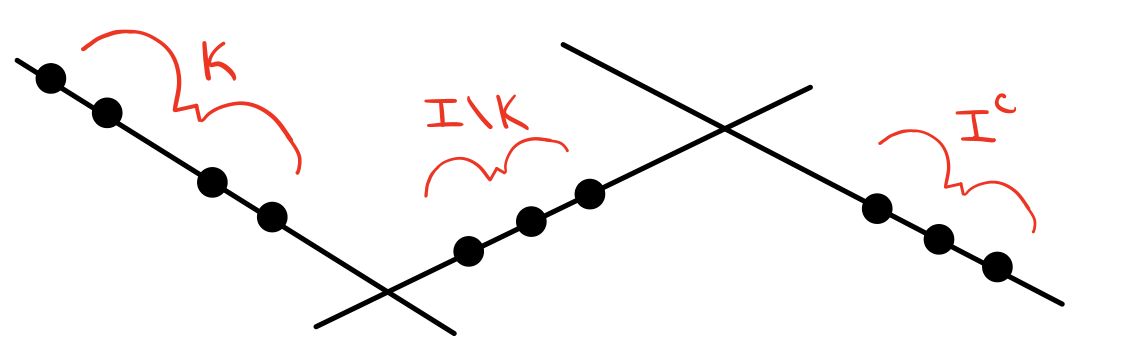
\includegraphics[width=.6\textwidth]{figures/fig-6.7.24.png}
\caption{只要 $K\subsetneq I$, 图中曲线就属于 $\delta_{0,\allowbreak I}\cap\delta_{0,\allowbreak K}$.}\label{src:6.7.24}\end{figure}
\begin{exercise}\label{src:6.7.25}
证明代数闭域 $k$ 上每条稳定曲线 $C$ 可形变为光滑曲线. 更精确地, 存在 $k$ 上连通曲线\footnote{依照约定, 曲线 (定义~\bookref{6.1.1}) 必在 $k$ 上有限型.} $T$ 上的稳定曲线族 $\pi:\mathcal C\to\allowbreak T$ 及点 $t\in T(k)$, 使 $\mathcal C_t\cong C$, $\pi^{-1}(T\setminus\{t\})\to\allowbreak T\setminus\{t\}$ 光滑.
\end{exercise}
逆命题, 即每条光滑曲线退化为稳定曲线, 更难.
\begin{proposition}\label{src:6.7.26}
设 $C$ 是特征 $0$ 代数闭域 $k$ 上光滑, 连通, 亏格 $g\geq2$ 的射影曲线. 则存在 $k$ 上光滑连通曲线 $T$ 上的稳定曲线族 $\mathcal C\to\allowbreak T$, 以及点 $s,\allowbreak t\in T(k)$, 使 $\mathcal C_s\cong C$, $\mathcal C_t$ 是有奇点的稳定曲线.
\end{proposition}
\begin{proof}
基本策略如下:
\begin{enumerate}[(1)]
\item 对 $d\gg0$, 选取 $d$ 次单分歧覆盖 $C\to\mathbb P^1$, 在互异点 $q_1,\allowbreak \ldots,\allowbreak q_b$ 上方分歧, $b=2g+2d-2$.
\item 将在 $q_i$ 上方分歧的覆盖形变为在一般点 $q'_i$ 上方分歧的 $C'\to\mathbb P^1$.
\item 将 $(\mathbb P^1,\allowbreak q'_i)\in M_{0,\allowbreak b}$ 退化为图~\bookref{6.7.27} 的稳定曲线 $(D,\allowbreak d_i)\in\overline M_{0,\allowbreak b}$.
\item 将覆盖 $C'\to\mathbb P^1$ 退化为在 $d_i$ 上方分歧的覆盖 $C''\to\allowbreak D$, 使 $C''$ 有奇点且稳定.
\end{enumerate}
\begin{figure}[H]\centering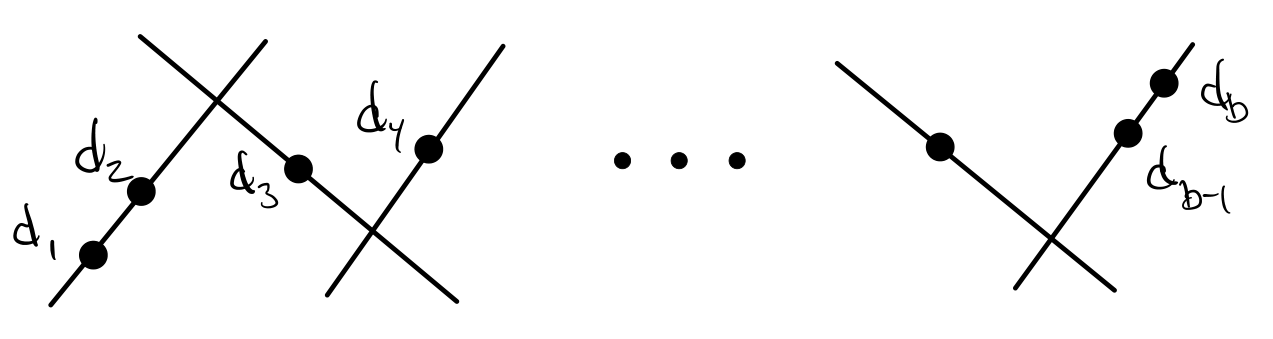
\includegraphics[width=.65\textwidth]{figures/fig-6.7.27.png}
\caption{退化曲线 $(D,\allowbreak d_i)\in\overline M_{0,\allowbreak b}$.}\label{src:6.7.27}\end{figure}
步骤 $1$ 的存在性由引理~\bookref{6.7.16} 保证, 并定义 $b$-点稳定曲线 $(\mathbb P^1,\allowbreak q_i)\in M_{0,\allowbreak b}$. 对其余步骤, 先断言只需在 $k$ 上有限型连通概形 $T$ 上找到族 $\mathcal C\to\allowbreak T$. 这表明 $C$ 与有奇点稳定曲线 $C''$ 位于 $\overline{\mathcal M}_g$ 的同一连通 (因而不可约) 分支 $\mathcal M'$. 由 Gabber 引理 (\bookref{5.6.1}), 有概形的有限覆盖 $Z\to\overline{\mathcal M}_g$, 且 $Z$ 有一个不可约分支 $Z'$ 满射到 $\mathcal M'$. $k$ 上有限型不可约概形 $Z'$ 的任意两个 $k$-点包含于整曲线 $Q\subseteq Z'$, 故考虑从 $Q$ 的正规化出发的 $\widetilde Q\to\allowbreak Z'\to\overline{\mathcal M}_g$ 即证断言.

步骤 $2$ 中, 令 $H\subseteq\operatorname{Hur}_{g,\allowbreak b}$ 为包含 $C\to\mathbb P^1$ 的连通分支. 因为 $\operatorname{Hur}_{g,\allowbreak b}\to\allowbreak M_{0,\allowbreak b}$ 有限平展 (习题~\bookref{6.7.13}(c)), 既开又闭, 复合 $H\hookrightarrow\operatorname{Hur}_{d,\allowbreak b}\to\allowbreak M_{0,\allowbreak b}$ 满射. $H$ 连通, 所以只需找到一个 $(C'\to\mathbb P^1)\in H$ 以及将 $C'$ 连到有奇点稳定曲线的连通基底上的稳定曲线族.

步骤 $3$: 断言存在交换图
\begin{equation}\label{src:6.7.28}
\begin{tikzcd}
T\setminus\{t\}\arrow[d]\arrow[r]&H\arrow[r,hook,"\text{开且闭}"]\arrow[dr]&\operatorname{Hur}_{g,b}\arrow[d,"\text{有限平展}"]\\
T\arrow[r,"{t\mapsto(D,d_i)}"']&\overline M_{0,b}&M_{0,b}\arrow[l,hook]
\end{tikzcd}
\end{equation}
其中 $T$ 光滑连通, $t$ 映到图~\bookref{6.7.27} 的稳定曲线. 因为 $\overline M_{0,\allowbreak b}$ 不可约 (命题~\bookref{6.7.23}), $M_{0,\allowbreak b}$ 稠密. 可选连通约化曲线的映射 $Y\to\overline M_{0,\allowbreak b}$ 及点 $y\in Y(k)$, 使 $y\mapsto(D,\allowbreak d_i)$, 每个其他点映到光滑曲线. 令 $Y'$ 为 $(Y\setminus\{y\})\times_{M_{0,\allowbreak b}}H$ 的连通分支, $T$ 为 $Y'\to\overline M_{0,\allowbreak b}$ 的像的闭包的正规化. 有 $t\in T$ 映到 $(D,\allowbreak d_i)$; 将 $T$ 换为 $t$ 的开邻域后, 可使 $T\setminus\{t\}\to\overline M_{0,\allowbreak b}$ 经过 $H$ 分解.

图~\bookeqref{6.7.28} 给出 $b$-点稳定亏格 $0$ 曲线族 $(\mathcal D\to\allowbreak T,\allowbreak \tau_i)$ 和 $T^*:=T\setminus\{t\}$ 上的单分歧覆盖 $\mathcal C^*\to\mathcal D^*$, 其中 $\mathcal D^*$ 为 $T^*$ 的原像, 截面 $\tau_i^*$ 选出分歧轨迹. 断言将 $(T,\allowbreak t)$ 换为分歧覆盖后, 存在虚线箭头补全 Cartesian 图
\[
\begin{tikzcd}
\mathcal C^*\arrow[r]\arrow[d,dashed]&\mathcal D^*\arrow[r]\arrow[d]&T^*\arrow[d]\\
\mathcal C\arrow[r,dashed,"f"']\arrow[ur,phantom,"\square"]&\mathcal D\arrow[r]\arrow[ur,phantom,"\square"]&T,
\end{tikzcd}
\]
其中 $\mathcal C\to\allowbreak T$ 是结点曲线族. 将 $\mathcal C$ 定义为 $\mathcal O_{\mathcal D}$ 在 $K(\mathcal C^*)$ 中的整闭包, 则 $f:\mathcal C\to\mathcal D$ 有限. 令 $\mathcal D^{\mathrm{sm}}=\mathcal D\setminus\{d_i\}$ 为相对光滑轨迹, 分歧轨迹的纯性 (\bookref{A.3.13}) 保证 $f^{-1}(\mathcal D^{\mathrm{sm}})\to\mathcal D^{\mathrm{sm}}$ 的分歧轨迹是除子. 因而 $\mathcal C\to\mathcal D$ 只在 $\tau_1,\allowbreak \ldots,\allowbreak \tau_b$ 以及可能在 $D=\mathcal D_t$ 的结点 $d_i$ 上方分歧. 为证 $\mathcal C\to\allowbreak S$ 为结点族, 注意在每个 $d_i$ 附近平展局部, 该映射形如有限态射 $U\to\allowbreak V:=\Spec k[x,\allowbreak y]/(xy-\pi^k)$, 其中 $k\leq d$, $\pi$ 是 $t\in T$ 的平展邻域上的局部坐标. $U\to\allowbreak V$ 在 $V\setminus0$ 上有限平展. 因为由 $(x',\allowbreak y')\mapsto(x'^k,\allowbreak y'^k)$ 定义的
\[
\Spec k[x',y']/(x'^ky'^k-\pi^k)\setminus0\to V\setminus0
\]
是泛覆盖, $V\setminus0$ 在 $U$ 中的原像必同构于 $\Spec k[x'',\allowbreak y'']/(x''^ly''^l-\pi^k)\setminus0$, 其中 $l\mid k$. 所以 $U=\Spec k[x'',\allowbreak y'']/(x''^ly''^l-\pi^k)$, 纤维 $U_t$ (由 $\pi=0$ 定义) 的约化概形结构仅有结点. 从而 $(\mathcal C_t)_{\mathrm{red}}$ 仅有结点. 用稳定约化 (\bookref{6.5.1}) 证明步骤 $4$ 的同一论证, 有分歧覆盖 $T'\to\allowbreak T$, 使 $\mathcal C'=\mathcal C\times_T T'$ 的正规化 $\widetilde{\mathcal C}'$ 的中心纤维约化且仅有结点. 将 $\mathcal C$ 换为 $\widetilde{\mathcal C}'$, $T$ 换为 $T'$, 便使 $\mathcal C\to\allowbreak T$ 成为结点曲线族.
\begin{figure}[H]\centering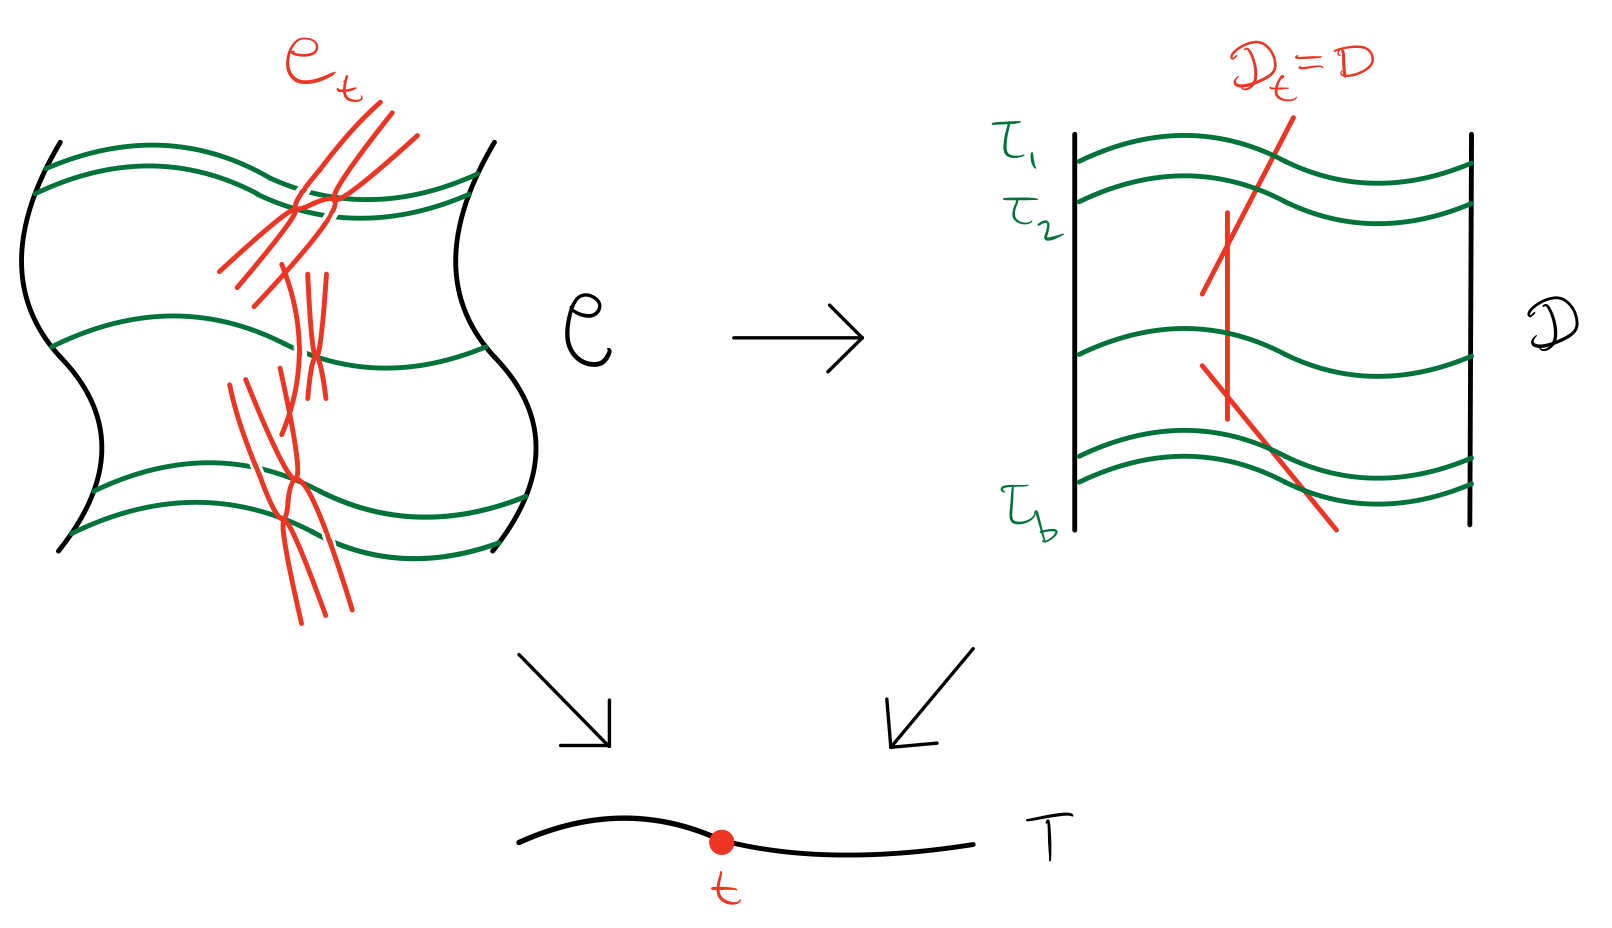
\includegraphics[width=.7\textwidth]{figures/fig-6.7.29.png}
\caption{$\mathcal C\to\mathcal D\to\allowbreak T$ 的示意图.}\label{src:6.7.29}\end{figure}
此族可能不稳定, 但由预稳定族的稳定收缩 (定理~\bookref{6.6.6}), 收缩有理尾和有理桥得到稳定族 $\mathcal C^{\mathrm{st}}\to\allowbreak T$. 为证 $C_0^{\mathrm{st}}$ 有奇点, 只需证 $C_0$ 的每个光滑不可约分支亏格为 $0$. 设 $X\subseteq C_0$ 为此分支, 它在 $C_0\to\mathcal D_0=D$ 下的像是其中一条 $\mathbb P^1$. 令诱导映射 $X\to\mathbb P^1$ 的次数为 $d'$. 它在标记点上方分歧, 并可能在该 $\mathbb P^1$ 所含 $D$ 的结点上方分歧, 分歧指数至多 $d'-1$. 若 $\mathbb P^1$ 位于链末端, 它含两个标记点和一个结点, Riemann--Hurwitz (\bookref{6.7.4}) 给出 $2g_X-2\leq-2d'+2+(d'-1)$, 推出 $g_X=0$. 若位于中间, 它含一个标记点和两个结点, 有 $2g_X-2\leq-2d'+1+2(d'-1)$, 也推出 $g_X=0$.
\end{proof}
\begin{theorem}[$\overline{\mathcal M}_{g,\allowbreak n}$ 的不可约性]\label{src:6.7.30}
设 $g,\allowbreak n$ 为非负整数, $2g-2+n>0$. 对每个特征 $0$ 域 $k$, $\overline{\mathcal M}_{g,\allowbreak n}$ 不可约, 并包含 $\mathcal M_{g,\allowbreak n}$ 作为非空稠密开子叠.
\end{theorem}
\begin{proof}
可假设 $k$ 代数闭. 每个亏格都有光滑曲线 (习题~\bookref{6.1.7}). 带 $n\geq3$ 个互异点的 $\mathbb P^1$ 稳定, 带 $n\geq1$ 个互异点的光滑连通射影亏格 $1$ 曲线也稳定, 所以只要 $2g-2+n>0$, $\mathcal M_{g,\allowbreak n}$ 非空. $\overline{\mathcal M}_{g,\allowbreak n}$ 光滑 (定理~\bookref{6.4.16}), 只需证连通. 因为 $\overline{\mathcal M}_{g,\allowbreak n+1}\to\overline{\mathcal M}_{g,\allowbreak n}$ 为泛族 (命题~\bookref{6.6.12}), $n$ 的连通性蕴涵每个 $n'>n$ 的连通性. 已知 $\overline{\mathcal M}_{0,\allowbreak n}$ 对 $n\geq3$ 连通 (命题~\bookref{6.7.23}). 又由习题~\bookref{4.1.21}(b), $\overline{\mathcal M}_{1,\allowbreak 1}\cong[(\mathbb A^2\setminus0)/\mathbb G_m]$ 连通, 故 $\overline{\mathcal M}_{1,\allowbreak n}$ 对 $n\geq1$ 连通.

只需证明 $g\geq2$ 时 $\mathcal M_g$ 连通, 由归纳可假设 $g'<g$ 时 $\overline{\mathcal M}_{g'}$ 连通. 每条光滑曲线退化为边界中的有奇点稳定曲线 (命题~\bookref{6.7.26}), 进一步只需证 $\overline{\mathcal M}_g$ 和 $\delta$ 连通. 利用粘合态射 (\bookref{6.6.16}), 写 $\delta=\delta_0\cup\cdots\cup\delta_{\lfloor g/2\rfloor}$, 其中
\[
\delta_0=\operatorname{im}(\overline{\mathcal M}_{g-1,2}\to\overline{\mathcal M}_g),\qquad
\delta_i=\operatorname{im}(\overline{\mathcal M}_{i,1}\times\overline{\mathcal M}_{g-i,1}\to\overline{\mathcal M}_g).
\]
由归纳假设, 各源连通, 故每个 $\delta_i$ 连通. 另一方面, 这些边界除子彼此相交: 对每个 $i,\allowbreak j=0,\allowbreak \ldots,\allowbreak \lfloor g/2\rfloor$, $\delta_i\cap\delta_j$ 包含图~\bookref{6.7.31} 的曲线. 另见~\cite{HM82} 中 Fulton 的附录.
\end{proof}
\begin{figure}[H]\centering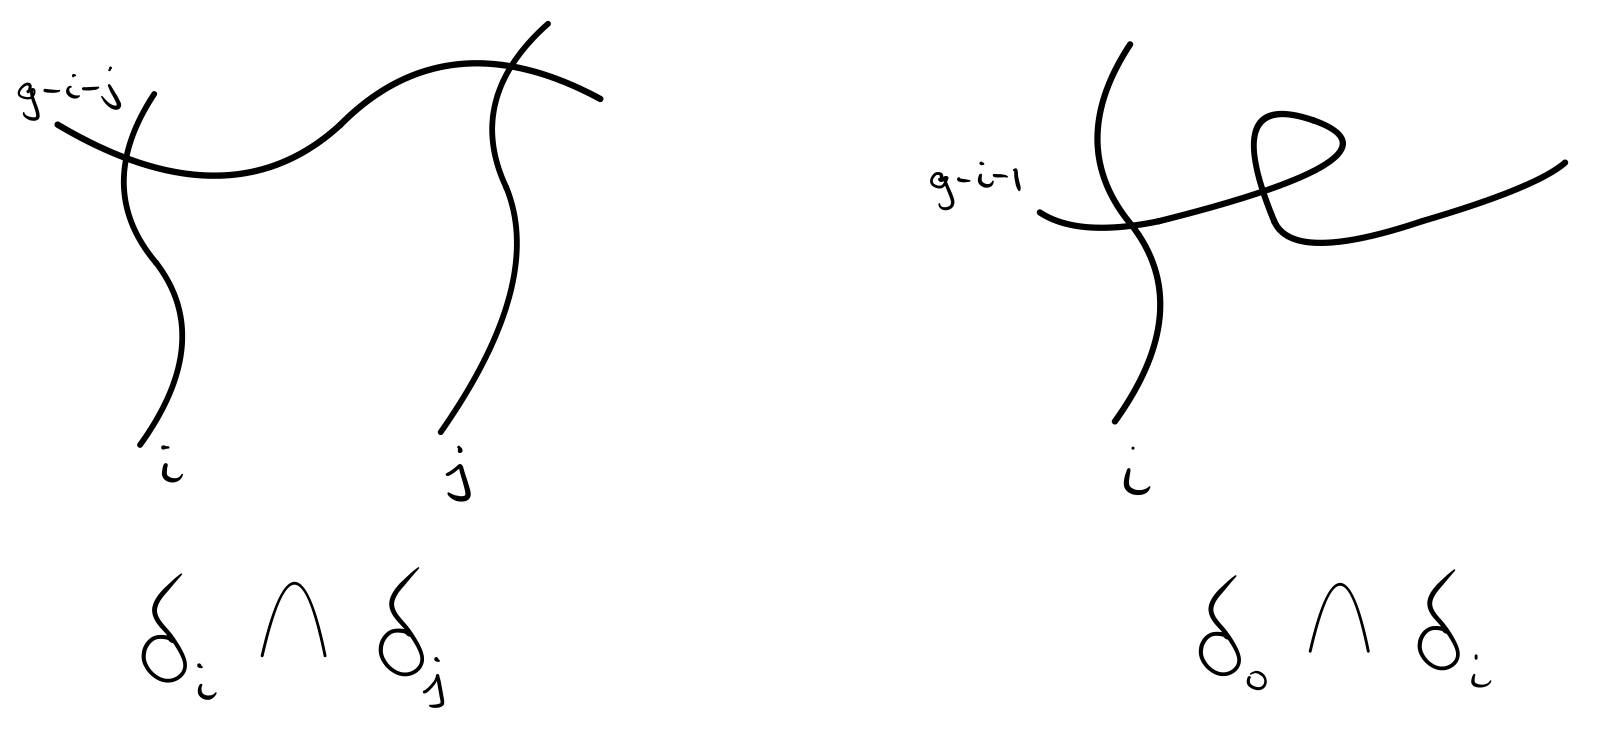
\includegraphics[width=.7\textwidth]{figures/fig-6.7.31.png}
\caption{边界除子 $\delta_i$ 与 $\delta_j$ 的交非空.}\label{src:6.7.31}\end{figure}
\begin{remark}[容许覆盖]\label{src:6.7.32}
上述论证受到 Harris 和 Mumford~\cite{HM82} 为计算 $\overline M_g$ 的 Kodaira 维数而引入的容许覆盖理论的启发. 另见~\cite[\S3.G]{HM98}. 容许覆盖推广单分歧覆盖 $C\to\mathbb P^1$, 允许源曲线和靶曲线具有结点. 其思想是定义模叠 $\overline{\mathcal{Hur}}_{g,\allowbreak b}$, 使其纳入图
\[
\begin{tikzcd}[column sep=small]
&\overline{\mathcal{Hur}}_{g,b}\arrow[dl]\arrow[dr]&\\
\overline{\mathcal M}_g&&\overline M_{0,b}
\end{tikzcd}
\quad\xleftarrow{\text{紧化}}\quad
\begin{tikzcd}[column sep=small]
&\operatorname{Hur}_{g,b}\arrow[dl]\arrow[dr]&\\
\mathcal M_g&&M_{0,b}.
\end{tikzcd}
\]
亏格 $g$ 的\newterm{容许覆盖}{admissible cover} 是从预稳定亏格 $g$ 曲线到稳定 $b$-点亏格 $0$ 曲线 $(B,\allowbreak p_1,\allowbreak \ldots,\allowbreak p_b)$ 的满射有限态射 $f:C\to\allowbreak B$, 满足:
\begin{enumerate}[(a)]
\item $B^{\mathrm{sm}}$ 的原像是 $C^{\mathrm{sm}}$, 诱导态射 $C^{\mathrm{sm}}\to\allowbreak B^{\mathrm{sm}}$ 为在 $p_i$ 上方单分歧的 $d$ 次覆盖, 即分歧指数均为 $2$, 每个纤维至多含一个分歧点;
\item 对每个结点 $q\in B$ 及其上方的每个结点 $r\in C$, $C\to\allowbreak B$ 在 $r$ 处的平展局部结构为 $k[x,\allowbreak y]/(xy)\to\allowbreak k[x,\allowbreak y]/(xy)$, 由 $(x,\allowbreak y)\mapsto(x^m,\allowbreak y^m)$ 定义; 即两个分支在结点处的分歧指数相等.
\end{enumerate}
定义推广到族, 给出固有 Deligne--Mumford 叠 $\overline{\mathcal{Hur}}_{g,\allowbreak b}$. (容许覆盖可有非平凡自同构群, 故此叠不是概形.) 对应 $(C\to\allowbreak B)\mapsto(B,\allowbreak p_i)$ 定义到 $\overline M_{0,\allowbreak b}$ 的态射. 对应 $(C\to\allowbreak B)\mapsto C^{\mathrm{st}}$ 定义到 $\mathcal M_g^{\mathrm{pre}}$ 的态射, 注意源曲线不必稳定. 与稳定收缩态射 (\bookref{6.6.7}) 复合, 得到到 $\overline{\mathcal M}_g$ 的态射.

可用此语言重写命题~\bookref{6.7.26} 的论证. 对 $d\gg0$ 和光滑曲线 $C$, 选取原像 $(C\to\mathbb P^1)\in\operatorname{Hur}_{g,\allowbreak b}$ (引理~\bookref{6.7.16}). 令 $H$ 为包含它的连通分支, $\overline H\subseteq\overline{\mathcal{Hur}}_{g,\allowbreak b}$ 为闭包. 因为 $\operatorname{Hur}_{g,\allowbreak b}\to\allowbreak M_{0,\allowbreak b}$ 有限平展, $\overline H$ 满射到 $\overline M_{0,\allowbreak b}$. 如命题~\bookref{6.7.26} 的证明选择交换图
\[
\begin{tikzcd}
T\setminus\{t\}\arrow[r]\arrow[d]&\overline H\arrow[d,"\text{固有}"]\\
T\arrow[r,"{t\mapsto(D,d_i)}"']&\overline M_{0,b},
\end{tikzcd}
\]
其中 $T$ 光滑连通, $t$ 映到图~\bookref{6.7.27} 的曲线, 某个 $t'\ne t$ 映到 $(C'\to\mathbb P^1)\in H$. 由固有性的赋值判据, 将 $T$ 换为分歧覆盖后, 存在提升 $T\to\overline H$, $t$ 映到容许覆盖 $(C''\to\allowbreak D)$. 如前证明, $C''$ 的每个光滑不可约分支的亏格为 $0$. 所以 $C'$ 退化为有奇点稳定曲线 $(C'')^{\mathrm{st}}$; 原覆盖与 $C'$ 的覆盖同处 Hurwitz 空间的一个连通分支, 故原曲线 $C$ 也退化为它. (构造覆盖族 $\mathcal C\to\mathcal D\to\allowbreak T$ 的论证也是证明容许覆盖叠固有性的关键步骤之一.)
\end{remark}
\subsection{正特征下的不可约性}\label{src:6.7.5-subsection}
遵循 Deligne--Mumford~\cite{DM69} 和 Fulton~\cite{Ful69} 的历史论证, 证明正特征下 $\overline{\mathcal M}_g$ 不可约. 核心是 Zariski 连通性定理 (\bookref{5.6.15}): 对 Noether Deligne--Mumford 叠之间的平坦固有态射, 纤维的几何连通分支数下半连续. 此定理在~\cite[定理 4.17]{DM69} 中陈述但未证明, 所需 Deligne--Mumford 叠理论之多令人惊讶.
\begin{theorem}[$\overline{\mathcal M}_{g,\allowbreak n}$ 的不可约性]\label{src:6.7.33}
若 $2g-2+n>0$, 则 $\overline{\mathcal M}_{g,\allowbreak n}$ 在任意域上不可约.
\end{theorem}
\begin{proof}
由定理~\bookref{6.7.19} 的超越证明或定理~\bookref{6.7.30} 的代数证明, 已知特征 $0$ 的情形, 只需证 $\overline{\mathbb F}_p$ 上的不可约性. 态射 $\overline{\mathcal M}_{g,\allowbreak n}\to\Spec\mathbb Z$ 光滑 (定理~\bookref{6.4.16}) 且固有 (定理~\bookref{6.5.23}), 故 Zariski 连通性定理 (\bookref{5.6.15}) 保证所有几何纤维的连通分支数相同. 由 $\overline{\mathbb Q}$ 上连通, 得到 $\overline{\mathbb F}_p$ 上连通, 从而不可约.
\end{proof}
\begin{remark}[Deligne 和 Mumford 的证明]\label{src:6.7.34}
上面是 Deligne 和 Mumford~\cite[\S5]{DM69} 给出的第二个论证. 请记住, 正是这篇非凡论文引入了叠 (今称 Deligne--Mumford 叠), 引入稳定曲线并证明稳定约化. 第一个不可约性论证~\cite[\S3]{DM69} 被他们称为``该定理的初等推导'', 与定理~\bookref{6.7.30} 利用光滑曲线的退化和边界的归纳结构的证明十分相近. 它依赖稳定约化与 $\mathcal M_g$ 的拓扑不可约性. 下面概述他们对任意域 $k$ 上不可约性的论证.

令 $H_g$ (分别地, $\overline H_g$) 为 $\operatorname{Hilb}^P(\mathbb P_{\mathbb Z}^{5g-6}/\mathbb Z)$ 中参数化光滑 (分别地, 稳定) 曲线的局部闭子概形. Mumford 在~\cite[定理 5.11, 7.13]{GIT} 中将 $\Spec\mathbb Z$ 上粗模概形 $M_g$ 构造为几何商 $H_g/\operatorname{PGL}_{5g-6}$, 并证明它对每个素数 $p$ 在 $\Spec\mathbb Z[1/p]$ 上拟射影. ($\overline{\mathcal M}_g$ 也有 $\Spec\mathbb Z$ 上的射影粗模概形 $\overline M_g$, 可认同为 $\overline H_g/\operatorname{PGL}_{5g-6}$, 但这是后来才证明的.)

\textbf{步骤 $1$: $M_g\times_{\mathbb Z}k$ 无在 $k$ 上固有的连通分支.}
令 $W(k)$ 为 $k$ 的 Witt 向量环; 它是完备 Noether 局部环, 一般点 $\eta$ 的特征为 $0$, 闭点 $0$ 的剩余域为 $k$. (例如 $W(\mathbb F_p)=\mathbb Z_p$ 是 $p$-进数环.) 由于 $M_g\times_{\mathbb Z}W(k)$ 拟射影, 可选包含它作为稠密开子概形的射影紧化
\[
\begin{tikzcd}
M_g\times_{\mathbb Z}W(k)\arrow[r,hook]\arrow[dr]&X\arrow[d,"\text{射影}"]\\
&\Spec W(k).
\end{tikzcd}
\]
由特征 $0$ 的结果, 一般纤维 $X_\eta$ 连通. $X$ 在 $W(k)$ 上平坦固有, 故概形的 Zariski 连通性定理 (\bookref{5.6.15}) 保证特殊纤维 $X_0$ 连通.

假设 $Y\subseteq M_g\times_{\mathbb Z}k$ 是 $k$ 上固有的连通分支. 它在 $X_0$ 中既开, 又因固有而闭. 由 $X_0$ 连通, $Y$ 必为整个 $M_g\times_{\mathbb Z}k$, 故后者固有且不可约. 为得矛盾, 令 $A_{g,\allowbreak k}$ 为主极化 $g$ 维阿贝尔簇模空间, 考虑将光滑曲线映为 Jacobian 的态射 $\Theta:M_g\times_{\mathbb Z}k\to\allowbreak A_{g,\allowbreak k}$, $C\mapsto\operatorname{Jac}(C)$. 固有性意味着像闭, 但当时已知像的闭包包含低维 Jacobian 的乘积.

\textbf{步骤 $2$: $\overline H_g\times_{\mathbb Z}k$ 无完全由光滑曲线组成的连通分支.}
令 $\overline H_g^{(1)},\allowbreak \ldots,\allowbreak \overline H_g^{(r)}$ 为其连通分支. 步骤 $1$ 保证每个 $H_g^{(i)}:=\overline H_g^{(i)}\cap(H_g\times_{\mathbb Z}k)$ 不固有. 因而有不延拓到 $\Delta=\Spec k[[t]]$ 的态射 $\Delta^*=\Spec k((t))\to\allowbreak H_g^{(i)}$. 由稳定约化 (\bookref{6.5.1}), 必要时将 $\Delta$ 换为分歧扩张后, 它延拓为 $\Delta\to\overline H_g^{(i)}$. 因而 $\overline H_g^{(i)}\setminus H_g^{(i)}$ 非空. 换言之, 每条光滑曲线退化为有奇点稳定曲线, 给出命题~\bookref{6.7.26} 的正特征证明.

\textbf{步骤 $3$: 边界 $\delta\times_{\mathbb Z}k$ 连通, 其中 $\delta=\overline M_g\setminus M_g$.}
由步骤 $2$, 后者蕴涵 $\overline M_g\times_{\mathbb Z}k$ 连通. 证明各 $\delta_i\times_{\mathbb Z}k$ 连通, 且每个两两交非空. 这正是定理~\bookref{6.7.30} 的证明利用亏格归纳, 粘合态射和图~\bookref{6.7.31} 中曲线所做的事. Deligne 和 Mumford 基本上给出相同论证, 但采用针对性技巧, 因为 $n$-点稳定曲线模空间与粘合态射的形式体系是 Knudsen 后来才引入的.

有趣的是, 两个证明均不本质依赖叠理论. 只要知道存在固有平坦的粗模空间 $\overline M_{g,\allowbreak n}\to\Spec\mathbb Z$, 第二个证明便成立. 但两个证明都根本依赖紧化 $\overline{\mathcal M}_g$ 与稳定约化.
\end{remark}
\begin{remark}[Fulton 的证明]\label{src:6.7.35}
Fulton~\cite{Ful69} 研究参数化在 $b$ 个无序点上方单分歧的 $d$ 次覆盖族 $\mathcal C\to\mathbb P^1_S$ 的变体 $\operatorname{Hur}_{g,\allowbreak b}^{\mathrm{rig,\allowbreak unord}}$ (见注记~\bookref{6.7.12}), 证明图
\[
\begin{tikzcd}
&\operatorname{Hur}_{g,b}^{\mathrm{rig,unord}}\arrow[dl]\arrow[dr,"\text{平展}"]&\\
\mathcal M_g&&\operatorname{Sym}^b\mathbb P^1\setminus\Delta=\mathbb P^b\setminus\Delta
\end{tikzcd}
\]
在 $\mathbb Z$ 上定义, 且 $d\geq g+1$ 时左方映射满射 (比推论~\bookref{6.7.18} 的界更好), 右方到 $M_{0,\allowbreak n}$ 的映射在 $\mathbb Z_{d!}$ 上有限平展, 即倒置所有素数 $p\leq d$ 后如此. Fulton 建立了``约化定理'': 若 $X$ 是完备离散赋值环 $R$ 上的光滑射影概形, $R$ 的剩余域 $k$ 代数闭, 分式域 $K$ 的特征为 $0$, $\Delta\subseteq X$ 是单纯相对除子 (即每个纤维无多重分支), 且有限平展覆盖 $Y\to\allowbreak X\setminus\Delta$ 满足 $Y_{\overline K}$ 不可约, 则 $Y_k$ 也不可约. 利用特征 $0$ 下 Hurwitz 空间不可约, 将此定理应用于 $\operatorname{Hur}_{g,\allowbreak b}^{\mathrm{rig,\allowbreak unord}}\to\operatorname{Sym}^b\mathbb P^1\setminus\Delta$, 得到特征 $p>d$ 下的不可约性. 取 $d=g+1$, 得到特征 $p>g+1$ 下 $\mathcal M_g$ 不可约.
\end{remark}

% Source printed pp. 279-292 / PDF pp. 287-300.
\section{Mumford 与 Gieseker 的射影性证明}\label{src:6.8}
\begin{epigraph}
毫不夸张地说, [定理 A] 在过去三十年的代数曲线理论中所起的基础性作用, 可与抽象曲线理论在此前六十年中的作用相比.
\epigraphauthor{Joe Harris 和 Ian Morrison~\cite[48 页]{HM98}}
\end{epigraph}
Mumford 在~\cite{GIT} 中发展几何不变量理论 (GIT), 用以构造代数几何中的商与模空间. 核心思想是将模叠 $\mathcal M$ (如 $\overline{\mathcal M}_g$) 表示为商叠 $[U/G]$, 其中 $G$ 约化, $U\subseteq\mathbb P(V)$ 为 $G$-表示 $V$ 的射影化的局部闭子概形, 并用 Hilbert--Mumford 判据 (\bookref{8.4.4}) 证明 $u\in\overline U$ 属于 $U$ 当且仅当它 GIT 稳定. 有趣的是, Mumford 首次将 $M_g$ 构造为 $\mathbb Z$ 上概形~\cite[定理 5.11, 7.13]{GIT}, 所用的是针对性技巧. 不久后, Mumford~\cite{Mum77} 和 Gieseker~\cite{Gie82} 用 GIT 将 $\overline M_g$ 构造为射影簇. 但 $\overline M_{g,\allowbreak n}$ 射影性的首个证明由 Knudsen 和 Mumford~\cite{KM76,Knu83a,Knu83b} 给出, 依赖到主极化阿贝尔簇模空间的 Satake 紧化的 Torelli 映射 $\overline M_g\to\overline A_g$.

本节在特征 $0$ 代数闭域 $k$ 上\footnote{构造如何推广到正特征和混合特征, 见注记~\bookref{6.8.7}.}, 将第~\bookref{8} 章发展的 GIT 应用于 Chow 概形和 Hilbert 概形, 介绍 Mumford 构造 $\overline M_g$ 的方法.
\subsection{利用 Chow 与 Hilbert 概形的 GIT 纲要}\label{src:6.8.1-subsection}
Hilbert 概形的 GIT 构造依赖两个整数, Chow 概形的构造只依赖 $k$:
\begin{itemize}
\item $k\geq5$, 定义多重典范嵌入的对偶化层倍数:
\[
|\omega_C^{\otimes k}|:C\hookrightarrow\mathbb P^{N_k},\qquad N_k=(2k-1)(g-1)-1.
\]
需要 $k\geq3$, 使稳定曲线 $C$ 的 $\omega_C^{\otimes k}$ 丰沛; 需要 $k\geq5$, 才使 Chow 或 Hilbert 概形的 GIT 构造给出 $\overline M_g$.
\item $m\gg0$, 将 $k$-典范嵌入曲线的 Hilbert 概形嵌入 Grassmann 簇所用方程的次数. 为得到嵌入, 需要 $m\gg0$.
\end{itemize}
\noindent\textbf{Hilbert 概形.} 对 $k>1$, 亏格 $g$ 的 $k$-多重典范嵌入稳定曲线的 Hilbert 多项式为 $P(t)=\chi(C,\allowbreak \omega_C^{\otimes kt})=(2kt-1)(g-1)$. Hilbert 概形 $\operatorname{Hilb}^P(\mathbb P^{N_k})$ 在 $k$ 上射影 (定理~\bookref{2.1.2}), 带 $\operatorname{PGL}_{N_k+1}$ 作用. 对 $k\geq3$, 有不变局部闭子概形 $U$, 使 $\overline{\mathcal M}_g\cong[U/\operatorname{PGL}_{N_k+1}]$ (习题~\bookref{6.4.17}). 令
\begin{equation}\label{src:6.8.1}
H:=\overline U\subseteq\operatorname{Hilb}^P(\mathbb P^{N_k}).
\end{equation}
由定理~\bookref{2.4.5}, 对 $m\gg0$, 有等变闭浸入
\[
\begin{aligned}
H&\hookrightarrow\operatorname{Gr}(P(m),\Gamma(\mathbb P^{N_k},\mathcal O(m))),\\
[C\subseteq\mathbb P^{N_k}]&\mapsto[\Gamma(\mathbb P^{N_k},\mathcal O(m))\twoheadrightarrow\Gamma(C,\mathcal O(m))].
\end{aligned}
\]
其中左方截面空间为 $\operatorname{Sym}^m\Gamma(C,\allowbreak \omega_C^{\otimes k})$, 若 $C\in U$, 右方为 $\Gamma(C,\allowbreak \omega_C^{\otimes mk})$. 由命题~\bookref{2.2.8}, Plücker 嵌入为
\[
\begin{aligned}
\operatorname{Gr}(P(m),\Gamma(\mathbb P^{N_k},\mathcal O(m)))&\hookrightarrow\mathbb P\Bigl(\bigwedge^{P(m)}\Gamma(\mathbb P^{N_k},\mathcal O(m))\Bigr),\\
[\Gamma(\mathbb P^{N_k},\mathcal O(m))\twoheadrightarrow\Gamma(C,\mathcal O(m))]
&\mapsto\Bigl[\bigwedge^{P(m)}\Gamma(\mathbb P^{N_k},\mathcal O(m))\twoheadrightarrow\bigwedge^{P(m)}\Gamma(C,\mathcal O(m))\Bigr].
\end{aligned}
\]
事实上, 对任意 $\operatorname{Hilb}^P(\mathbb P^n)$, $m\gg0$ 时有 $\operatorname{PGL}_{n+1}$-等变闭浸入
\[
\operatorname{Hilb}^P(\mathbb P^n)\hookrightarrow\operatorname{Gr}(P(m),\Gamma(\mathbb P^n,\mathcal O(m)))
\hookrightarrow\mathbb P\Bigl(\bigwedge^{P(m)}\Gamma(\mathbb P^n,\mathcal O(m))\Bigr).
\]
研究不必多重典范嵌入的曲线的稳定性同样容易. 令 $\mathcal O_{\operatorname{Gr}}(1)$ 为 Grassmann 簇上的甚丰沛线丛, 令 $L_m=\mathcal O_{\operatorname{Gr}}(1)|_{\operatorname{Hilb}^P(\mathbb P^n)}$. 注意它依赖 $m$. 对 $m\gg0$, $L_m$ 甚丰沛, 继承 $\operatorname{PGL}_{n+1}$ 作用, 因而也继承 $\operatorname{GL}_{n+1}$ 和 $\operatorname{SL}_{n+1}$ 作用. 稍后限制到 $\operatorname{SL}_{n+1}$ 的单参数子群, 但同时考虑 $\lambda=\operatorname{diag}(\lambda_i)$, $\sum\lambda_i\ne0$ 也有用.
\begin{definition}\label{src:6.8.2}
对单参数子群 $\lambda:\mathbb G_m\to\operatorname{GL}_{n+1}$, 将 $[C\subseteq\mathbb P^n]$ 的 Hilbert--Mumford 指数 (定义~\bookref{8.4.1}) 记为 $\mu_{L_m}^{\mathrm{Hilb}}(C,\allowbreak \lambda)$.
\end{definition}
单项式 $x_0^{m_0}\cdots x_n^{m_n}$ 的 $\lambda$-权为 $\sum_i m_i\lambda_i$, 多项式的 $\lambda$-权为其中单项式的最大权. 对多项式集 $\beta=\{f_1,\allowbreak \ldots,\allowbreak f_p\}$, 记其权为各多项式权之和. 以下将 $\lambda$-权简记为 $\operatorname{wt}_\lambda$. 有
\begin{equation}\label{src:6.8.3}
\mu_{L_m}^{\mathrm{Hilb}}(C,\lambda)=\min_\beta\operatorname{wt}_\lambda(\beta),
\end{equation}
其中 $\beta\subseteq\Gamma(\mathbb P^n,\allowbreak \mathcal O_{\mathbb P^n}(m))$ 映到 $\Gamma(C,\allowbreak \mathcal O_C(m))$ 的基.

\noindent\textbf{Chow 概形.} 次数 $d$ 的整曲线 $C\subseteq\mathbb P^n$ 的 Chow 形式 $f_C\in\operatorname{Sym}^d(k^{n+1})^{\otimes2}$ 定义于~\bookref{2.4.5-subsection} 节. 它在变量 $u_{0i}$, $u_{1i}$ ($i=0,\allowbreak \ldots,\allowbreak n$) 中各为 $d$ 次多齐次多项式, 使 $f_C(a_0,\allowbreak b_0,\allowbreak \ldots,\allowbreak a_n,\allowbreak b_n)=0$ 当且仅当
\[
C\cap\{a_0x_0+\cdots+a_nx_n=0\}\cap\{b_0x_0+\cdots+b_nx_n=0\}\ne\varnothing.
\]
定义推广到次数 $d$ 的有效 $1$-圈; Chow 概形 $\operatorname{Chow}_{1,\allowbreak d}(\mathbb P^n)\subseteq\mathbb P(\operatorname{Sym}^d(k^{n+1})^{\otimes2})$ 是所有此类 Chow 形式轨迹的闭包.
\begin{definition}\label{src:6.8.4}
对单参数子群 $\lambda:\mathbb G_m\to\operatorname{GL}_{n+1}$, 将次数 $d$ 的约化曲线 $C\subseteq\mathbb P^n$ 的 Chow 形式的 Hilbert--Mumford 指数记为 $\mu^{\mathrm{Chow}}(C,\allowbreak \lambda)$.
\end{definition}
对整曲线的 Chow 形式及每个 $t\in\mathbb G_m(k)$, 可写
\[
f_{\lambda(t)\cdot C}=\lambda(t)\cdot f_C=\sum_{i=\mu}^\nu t^if_{C,i}\in k[t,u_{i,j}],
\]
其中 $f_{C,\allowbreak i}$ 的权为 $i$, 假设 $f_{C,\allowbreak \mu}\ne0$. 则 $\lim_{t\to0}\lambda(t)\cdot f_C=f_{C,\allowbreak \mu}$, $\mu^{\mathrm{Chow}}(C,\allowbreak \lambda)=\mu$.

\noindent\textbf{Chow, Hilbert 与渐近 Hilbert 稳定性.} 称曲线 $C\subseteq\mathbb P^n$
\begin{itemize}
\item \newterm{Chow 稳定}{Chow stable}/半稳定, 若 Chow 形式对 $\operatorname{SL}_{n+1}$ 作用稳定/半稳定;
\item $m$-Hilbert 稳定/半稳定, 若 Hilbert 概形中的点对 $\operatorname{SL}_{n+1}$ 作用及线丛 $L_m$ 稳定/半稳定;
\item \newterm{渐近 Hilbert 稳定}{asymptotically Hilbert stable}/半稳定, 若对 $m\gg0$ 是 $m$-Hilbert 稳定/半稳定的.
\end{itemize}
GIT 构造依赖下列稳定性分析.
\begin{theorem}\label{src:6.8.5}
设 $k\geq5$.
\begin{enumerate}[(1)]
\item 由完全线性系 $|\omega_C^{\otimes k}|$ 嵌入的光滑曲线 $C\subseteq\mathbb P^{N_k}$ 是 Chow 稳定的.
\item 若 $[C\subseteq\mathbb P^{N_k}]$ 是光滑 $k$-多重典范嵌入曲线轨迹的闭包中的 Chow 半稳定曲线, 则 $C$ 是 $k$-多重典范嵌入的 (Deligne--Mumford) 稳定曲线.
\end{enumerate}
此外, 存在 $m\gg0$, 使每条此类光滑曲线 $m$-Hilbert 稳定, 并使 $H$ 中每条 $m$-Hilbert 半稳定曲线均为 $k$-多重典范嵌入稳定曲线.
\end{theorem}
几点说明:
\begin{itemize}
\item (1) 在概念上最困难, 因为需对每个单参数子群检验指数为负. 但 Mumford 将指数解释为 $\mathbb A^1\times C$ 上理想的重数 $e(C,\allowbreak \lambda)$ (\bookref{6.8.2-subsection} 节), 给出了简洁证明. 此重数可由 $C$ 上的重数估计 (命题~\bookref{6.8.19}), 足以检验光滑曲线稳定性 (定理~\bookref{6.8.22}).
\item 此界不足以直接证明稳定曲线的 Chow 稳定性. 尽管如此, (1), (2) 足以间接得出它.
\item (2) 概念上较容易, 只需找出使曲线去稳定化的单参数子群, 但技术上最繁重. \bookref{6.8.5-subsection} 节仅验证部分细节, 更完整论述请见所引文献.
\end{itemize}
由此可完成定理~\hyperref[thm:A]{A} 的证明.
\begin{theorem}\label{src:6.8.6}
在特征 $0$ 域上, 若 $2g-2+n>0$, 则粗模空间 $\overline M_{g,\allowbreak n}$ 射影.
\end{theorem}
\begin{proof}
由定理~\bookref{6.5.23}, $\overline{\mathcal M}_{g,\allowbreak n}$ 是有固有粗模空间 $\overline M_{g,\allowbreak n}$ 的固有 Deligne--Mumford 叠. 遗忘态射是泛族 (命题~\bookref{6.6.12}), 因而源上有相对丰沛线丛 $L$ (可取相对对偶化层扭以泛截面之和). 由习题~\bookref{5.4.29}(2), $L$ 下降为 $\overline M_{g,\allowbreak n+1}$ 上相对于 $\overline M_{g,\allowbreak n}$ 丰沛的线丛. 故只需证明 $g\geq2$ 时 $\overline M_g$ 射影. 已知 $\overline M_{0,\allowbreak 3}=\Spec k$, $\overline M_{1,\allowbreak 1}=\mathbb P^1$ 射影.

对 $k\geq5$, 置 $P(t)=(2kt-1)(g-1)$, $N_k+1=\mathrm h^0(C,\allowbreak \omega_C^{\otimes k})=(2k-1)(g-1)$. 由习题~\bookref{6.4.17}, 写 $\overline{\mathcal M}_g=[U/\operatorname{PGL}_{N_k+1}]$. 令 $H=\overline U$, 需证存在 $m\gg0$ 使 $U=H_{L_m}^s$. 对 $\operatorname{PGL}_{N_k+1}$ 与 $\operatorname{SL}_{N_k+1}$ 的稳定性相同, 因为两群间映射有有限余核, 单参数子群在伸缩意义下相同, Hilbert--Mumford 判据对一群成立当且仅当对另一群成立.

应用定理~\bookref{6.8.5} 后, 还需证每条 $k$-多重典范嵌入稳定曲线 $C$ 是 $m$-Hilbert 稳定的. 取离散赋值环 $R$ 上一般光滑的稳定族 $\mathcal C\to\Spec R$, 中心纤维为 $C$. 一般纤维光滑, 所以 $m$-Hilbert 稳定. 由 GIT 中的半稳定约化 (注记~\bookref{8.1.4}), 必要时扩张 $R$ 后, 存在一般纤维与原族同构的 $m$-Hilbert 半稳定曲线族 $\mathcal C'\to\Spec R$. 中心纤维半稳定, 故为稳定曲线. 两个稳定曲线族一般同构, $\overline{\mathcal M}_g$ 的分离性 (命题~\bookref{6.5.20}) 给出 $\mathcal C\cong\mathcal C'$. 所以 $C=\mathcal C_0=\mathcal C'_0$ 是 $m$-Hilbert 稳定的, 即 $U=H_{L_m}^s$. 应用 GIT 第一基本定理 (\bookref{8.2.6}), 得到射影几何商 $U/\operatorname{PGL}_{N_k+1}$. 因而 $[U/\operatorname{PGL}_{N_k+1}]\to\allowbreak U/\operatorname{PGL}_{N_k+1}$ 是粗模空间; 由唯一性, $\overline M_g$ 为此射影商.

也可用 $\operatorname{Chow}_{1,\allowbreak d}(\mathbb P^{N_k})$, $d=2k(g-1)$, 及光滑 $k$-多重典范嵌入曲线轨迹的闭包 $Z$. 写 $\mathcal M_g=[U/\operatorname{PGL}_{n+1}]$, $U\subseteq Z$ 为 $k$-多重典范嵌入稳定曲线的轨迹; 例如可由 Hilbert 到 Chow 的态射 $Z\to\allowbreak H$ 在结点曲线轨迹上是同构得出. 同一论证表明 $U=Z^s$, 且 $\overline{\mathcal M}_g\to\allowbreak Z^s/\operatorname{PGL}_{n+1}$ 有射影粗模空间. 另见~\cite[推论 5.2]{Mum77}, \cite[定理 2.0.2]{Gie82} 和~\cite[推论 4.42]{HM98}.
\end{proof}
\begin{remark}\label{src:6.8.7}
特征 $0$ 的限制是因为第~\bookref{8} 章仅对线性约化群发展 GIT. GIT 同样适用于正特征的约化群 (见注记~\bookref{7.5.4}), 甚至 $\mathbb Z$ 上的约化群概形~\cite{Ses77}. 定理~\bookref{6.8.5} 在任意特征成立, 因而可将 $\overline M_g$ 构造为 $\mathbb Z$ 上的射影概形.

直接验证稳定曲线 Chow 稳定性的 GIT 构造较近才在~\cite{BS08,LW15} 中完成, 并处理标记点的情形. 任意极化曲线 (不必多重典范嵌入) 的稳定性分析见~\cite{Cap94,BFMV14}.
\end{remark}
\subsection{Hilbert--Mumford 指数的解释}\label{src:6.8.2-subsection}
将两个指数认同为其他代数几何不变量, 得到实用的稳定性判据 (命题~\bookref{6.8.17}), 下一节用它证明光滑曲线稳定性. 为简单起见, 以下限于一维, 虽然很多论证可推广到任意维.

\noindent\textbf{理想层 $J_\lambda\subseteq\mathcal O_{C\times\mathbb A^1}$.} 设 $C\subseteq\mathbb P^n$ 为曲线; 稍后取 $n=N_k$. 令 $\lambda(t)=\operatorname{diag}(t^{\lambda_0},\allowbreak \ldots,\allowbreak t^{\lambda_n})$, $\lambda_0\geq\cdots\geq\lambda_n=0$. 对 $\mathbb P^n$ 的坐标 $x_i$ 和 $\mathbb A^1$ 的坐标 $t$, 定义 $J_\lambda=(t^{\lambda_i}x_i)$. 有理映射 $(t,\allowbreak x)\mapsto\lambda(t)\cdot x$ 通过爆破 $J_\lambda$ 消解, 给出交换图
\[
\begin{tikzcd}
&\operatorname{Bl}_{J_\lambda}(C\times\mathbb A^1)\arrow[dl]\arrow[dr]&\\
\mathbb A^1\times C\arrow[dr]& &\mathcal X\arrow[r,hook]\arrow[dl]&\mathbb A^1\times\mathbb P^n\\
&\mathbb A^1&&
\end{tikzcd}
\]
其中 $\mathcal X$ 是右上映射的概形论像. 投影 $\mathcal X\to\mathbb A^1$ 平坦, 中心纤维为 Hilbert 概形中的极限 $\lim_{t\to0}\lambda(t)\cdot[C\subseteq\mathbb P^n]$; 见注记~\bookref{2.4.4} 中固有性赋值判据的证明. $\mathcal X_0$ 被 $\mathbb G_m$ 固定, $\Gamma(\mathcal X_0,\allowbreak \mathcal O_{\mathcal X_0}(m))$ 对每个 $m$ 带 $\mathbb G_m$ 作用.

\noindent\textbf{Hilbert 函数的渐近权.} $\operatorname{GL}_{n+1}$-表示 $V$ 的 $\lambda$-权为 $\operatorname{wt}_\lambda(V)=\sum_i i\dim_kV_i$, $V_i$ 为诱导 $\mathbb G_m$ 作用的第 $i$ 个特征空间.
\begin{definition}[$r(C,\allowbreak \lambda)$]\label{src:6.8.8}
对曲线 $C\subseteq\mathbb P^n$ 和整数权 $\lambda_i$ 定义的单参数子群, 将 $r(C,\allowbreak \lambda)$ 定义为 $m\gg0$ 时二次多项式
\[
\operatorname{wt}_\lambda\Gamma(\mathcal X_0,\mathcal O_{\mathcal X_0}(m))
=r(C,\lambda)\frac{m^2}{2}+c_1m+c_0
\]
的归一化首项系数.
\end{definition}
$r(C,\allowbreak \lambda)$ 在 $m\gg0$ 时是二次多项式, 因而良定义, 是定理~\bookref{6.8.11} 的推论. 此定义类似于 K-稳定性中的 Futaki 不变量 (见~\bookref{10.1.4-subsection} 节); K-稳定性对应于渐近 Chow 稳定性, 即 $k\gg0$ 时多重典范嵌入的 Chow 稳定性.

\noindent\textbf{与加权旗标的接触重数.} 若 $\mathcal X$ 是 $k$ 上分离有限型二维概形, 理想层 $J$ 定义 $k$ 上固有的子概形, $L$ 是 $\mathcal X$ 上的线丛, 则 Euler 特征
\begin{equation}\label{src:6.8.9}
\chi(\mathcal X,L^{\otimes m}/J^mL^{\otimes m})=e_L(J)\frac{m^2}{2}+\text{低次项}
\end{equation}
为有理系数二次多项式. 其归一化首项系数 $e_L(J)$ 称为以 $L$ 度量的 $J$ 的重数. 这是 Hilbert--Samuel 多项式的特例; 见~\cite{Ram74}, \cite[命题 2.1]{Mum77} 和~\cite[\S12.1]{Eis95}.

若 $J=0$, $L$ 甚丰沛, 此多项式是 Hilbert 多项式, $e_L(0)$ 是 $\mathcal X$ 的次数. 若 $L=p^*\mathcal O_{\mathbb P^m}(1)$ 来自映射 $p:\mathcal X\to\mathbb P^n$, 则 $e_L(0)$ 是像定义的 Chow 圈的次数 (系数照常由函数域扩张次数定义). 若 $J$ 定义支撑在一点的子概形, 则 $e_L(J)$ 是奇点重数. 重数如何度量线性投影下的次数差, 见命题~\bookref{6.8.21}. 理想 $J_\lambda$ 只在 $\lambda_i\geq0$ 时有定义, 因而下述 $e(C,\allowbreak \lambda)$ 也要求此条件.
\begin{definition}[$e(C,\allowbreak \lambda)$]\label{src:6.8.10}
设 $C\subseteq\mathbb P^n$, 单参数子群的权满足 $\lambda_0\geq\cdots\geq\lambda_n\geq0$. 定义
\[
e(C,\lambda)=e_{\mathcal O_{\mathbb A^1}\boxtimes\mathcal O_C(1)}(J_\lambda),
\]
即以 $\mathcal O_{\mathbb A^1}\boxtimes\mathcal O_C(1)$ 度量的理想层 $J_\lambda=(t^{\lambda_i}x_i)$ 的重数.
\end{definition}
单参数子群定义加权旗标
\[
\underbrace{\{x_1=\cdots=x_n=0\}}_{L_0,\ \text{权 }\lambda_0}
\subseteq\underbrace{\{x_2=\cdots=x_n=0\}}_{L_1,\ \text{权 }\lambda_1}
\subseteq\cdots\subseteq\underbrace{\{x_n=0\}}_{L_{n-1},\ \text{权 }\lambda_{n-1}}\subseteq\mathbb P^n.
\]
粗略地说, $J_\lambda$ 定义的闭子概形是各 $L_i\cap C$ 的 $\lambda_i$ 阶加厚的并, $e(C,\allowbreak \lambda)$ 度量加权旗标与 $C$ 的接触程度.

\noindent\textbf{Hilbert--Mumford 指数的等价解释.}
\begin{theorem}\label{src:6.8.11}
设 $C\subseteq\mathbb P^n$, 单参数子群的整数权为 $\lambda_0\geq\cdots\geq\lambda_n$. 则 $\mu^{\mathrm{Chow}}(C,\allowbreak \lambda)=r(C,\allowbreak \lambda)$. 若每个 $\lambda_i\geq0$, 则 $\mu^{\mathrm{Chow}}(C,\allowbreak \lambda)=r(C,\allowbreak \lambda)=e(C,\allowbreak \lambda)$.
\end{theorem}
\begin{proof}
先归结到直线并, 再到一条直线. 若 $C$ 是直线, 可换坐标使 $C=V(x_2,\allowbreak \ldots,\allowbreak x_n)$. 直接计算 Chow 形式为 $u_{00}u_{11}-u_{01}u_{10}$, 指数为 $\lambda_0+\lambda_1$. 因为 $\Gamma(C,\allowbreak \mathcal O(m))=\langle x_0^m,\allowbreak x_0^{m-1}x_1,\allowbreak \ldots,\allowbreak x_1^m\rangle$, 权为 $(\lambda_0+\lambda_1)\binom{m+1}{2}$, 故 $r(C,\allowbreak \lambda)=\lambda_0+\lambda_1$. 若 $C$ 集合论上包含于坐标直线 $L_{ij}=V(x_0,\allowbreak \ldots,\allowbreak \widehat x_i,\allowbreak \ldots,\allowbreak \widehat x_j,\allowbreak \ldots,\allowbreak x_n)$ 的并, 令 $a_{ij}$ 为一般点处的重数. 两不变量只依赖这些一般点处的概形结构, 不依赖嵌入点. 由 $f_C=\prod_{ij}f_{L_{ij}}^{a_{ij}}$, 指数等于 $\sum_{ij}a_{ij}\mu^{\mathrm{Chow}}(L_{ij},\allowbreak \lambda)$. 等式 $r(X,\allowbreak \lambda)=\sum_{ij}a_{ij}r(L_{ij},\allowbreak \lambda)$ 留给读者; 由直线情形得到结论.

两不变量均由 Hilbert 概形中的极限曲线决定, 故可假设 $C$ 被 $\lambda$ 固定. 极大环面 $\mathbb G_m^{n+1}$ 作用于固有 Hilbert 概形, 因为环面可解, Borel 不动点定理 (参见~\cite[推论 17.3]{Mil17}) 保证轨道闭包包含环面固定点 $[\mathcal X_0\subseteq\mathbb P^{n+1}]$, 必集合论地包含于坐标直线并. 得到图
\[
\begin{tikzcd}
\mathcal X_0\arrow[r,hook]\arrow[d]&\mathcal X\arrow[d]&C\arrow[l,hook]\arrow[d]\\
0\arrow[r]&\mathbb A^1&1\arrow[l],
\end{tikzcd}
\]
其中 $\mathcal X\subseteq\mathbb P^n\times\mathbb A^1$ 为 $\mathbb G_m$-不变闭子概形 ($\mathbb P^n$ 上作用为 $\lambda$, $\mathbb A^1$ 上作用平凡), $\mathcal X\to\mathbb A^1$ 是等变平坦族, 在 $1$ 处为 $C$, 在 $0$ 处为 $\mathcal X_0$. 验证 $\mu(C,\allowbreak \lambda)=\mu(\mathcal X_0,\allowbreak \lambda)$, $r(C,\allowbreak \lambda)=r(\mathcal X_0,\allowbreak \lambda)$ 留给读者.

现假设权非负, 证明 $e=r$. 写 $\mathcal X=\operatorname{Proj}\bigoplus_{m\geq0}R_m$, 其中 $R_m$ 为 $k[t]\otimes_k\mathrm H^0(C,\allowbreak \mathcal O_C(m))$ 中由 $t^{\lambda_i}x_i$ 的 $m$ 次多项式生成的 $k[t]$-子模. 以下将``归一化首项系数''简记为 $\operatorname{nlc}$. 有
\begin{equation}\label{src:6.8.12}
\begin{aligned}
r(C,\lambda)&=\operatorname{nlc}\operatorname{wt}_\lambda\mathrm H^0(\mathcal X_0,\mathcal O_{\mathcal X_0}(m))\\
&=\operatorname{nlc}\operatorname{wt}_\lambda(R_m/tR_m)\\
&=\operatorname{nlc}\dim_k\bigl((k[t]\otimes_k\mathrm H^0(C,\mathcal O_C(m)))/R_m\bigr).
\end{aligned}
\end{equation}
末等式由引理~\bookref{6.8.14} 得到, 对所有 $m$ 成立. 另一方面, 置 $X=\mathbb A^1\times C$, $L=\mathcal O_{\mathbb A^1}\boxtimes\mathcal O_C(1)$, 定义给出 $e(C,\allowbreak \lambda)=\operatorname{nlc}\chi(X,\allowbreak L^{\otimes m}/J_\lambda^mL^{\otimes m})$. 读者可验证
\begin{equation}\label{src:6.8.13}
\begin{aligned}
e(C,\lambda)&=\operatorname{nlc}\mathrm h^0(X,L^{\otimes m}/J_\lambda^mL^{\otimes m})\\
&=\operatorname{nlc}\dim_k\bigl(\mathrm H^0(X,L^{\otimes m})/\mathrm H^0(X,J_\lambda^mL^{\otimes m})\bigr)\\
&=\operatorname{nlc}\dim_k\bigl((k[t]\otimes_k\mathrm H^0(C,\mathcal O_C(m)))/R_m\bigr).
\end{aligned}
\end{equation}
故 $r=e$. 另见~\cite[命题 2.6, 定理 2.9]{Mum77}.
\end{proof}
关键是将依赖极限曲线的 $\operatorname{wt}_\lambda(R_m/tR_m)$, 与曲面 $\mathbb A^1\times C$ 上定义的商空间维数认同.
\begin{lemma}\label{src:6.8.14}
设 $V$ 是维数 $n$ 的 $\mathbb G_m$-表示, 权为 $\lambda_n\geq\cdots\geq\lambda_0\geq0$. 令 $V_i$ 为权 $\lambda_i$ 的特征空间, $R\subseteq k[t]\otimes V$ 为由 $t^{\lambda_i}V_i$ ($i=0,\allowbreak \ldots,\allowbreak n$) 生成的 $k[t]$-子模. 则 $\operatorname{wt}_\lambda(R/tR)=\dim_k((k[t]\otimes V)/R)$.
\end{lemma}
\begin{proof}
写 $k[t]\otimes V=\bigoplus_{i,\allowbreak d}t^dV_i$, $R/tR$ 由 $t^{\lambda_i}V_i$ 自由生成, 商由 $V_i,\allowbreak tV_i,\allowbreak \ldots,\allowbreak t^{\lambda_i-1}V_i$ 自由生成, 故两边均为 $\sum_i\lambda_i\dim V_i$.
\end{proof}
\begin{exercise}[细节]\label{src:6.8.15}
补全定理~\bookref{6.8.11} 证明中省略的细节.
\end{exercise}
Hilbert 指数也有优美解释, 可与 Chow 指数比较.
\begin{proposition}\label{src:6.8.16}
设 $C\subseteq\mathbb P^n$, 单参数子群的权为 $\lambda_0\geq\cdots\geq\lambda_n\geq0$. 对 $m\gg0$,
\[
\mu_{L_m}^{\mathrm{Hilb}}(C,\lambda)
=\dim_k\bigl(\mathrm H^0(\mathbb A^1\times C,\mathcal O_{\mathbb A^1}\boxtimes\mathcal O_C(m))/R_m\bigr),
\]
其中 $R_m$ 由 $t^{\lambda_i}x_i$ 的 $m$ 次单项式生成, 而 $\mu^{\mathrm{Chow}}(C,\allowbreak \lambda)$ 是此维数的归一化首项系数. 特别地, 它是 $\mu_{L_m}^{\mathrm{Hilb}}(C,\allowbreak \lambda)$ 的归一化首项系数.
\end{proposition}
\begin{proof}
写 $R_m=\bigoplus_{i\geq0}R_{m,\allowbreak i}t^i\subseteq\bigoplus_{i\geq0}\mathrm H^0(C,\allowbreak \mathcal O_C(m))t^i$. 有 $R_{m,\allowbreak 0}\subseteq R_{m,\allowbreak 1}\subseteq\cdots\subseteq R_{m,\allowbreak I}=\mathrm H^0(C,\allowbreak \mathcal O_C(m))$ ($I\gg0$). 由~\bookeqref{6.8.3}, 最小权的基先选择 $R_{m,\allowbreak 0}$ 的基, 再依次扩充为 $R_{m,\allowbreak i}$ 的基. 故
\[
\begin{aligned}
\mu_{L_m}^{\mathrm{Hilb}}(C,\lambda)
&=0\dim R_{m,0}+1(\dim R_{m,1}-\dim R_{m,0})\\
&\quad+2(\dim R_{m,2}-\dim R_{m,1})+\cdots\\
&=I\dim\mathrm H^0(C,\mathcal O_C(m))-\sum_{i=0}^{I-1}\dim R_{m,i}\\
&=\sum_{i=0}^{I-1}\dim\bigl(\mathrm H^0(C,\mathcal O_C(m))/R_{m,i}\bigr)\\
&=\dim_k\bigl(\mathrm H^0(\mathbb A^1\times C,\mathcal O_{\mathbb A^1}\boxtimes\mathcal O_C(m))/R_m\bigr).
\end{aligned}
\]
最后结论由~\bookeqref{6.8.12} 得到. 另见~\cite[命题 3.2]{Mor80}.
\end{proof}
\subsection{Chow 与 Hilbert 稳定性判据}\label{src:6.8.3-subsection}
\begin{proposition}[Chow 稳定性判据]\label{src:6.8.17}
曲线 $C\subseteq\mathbb P^n$ Chow 稳定 (分别地, 半稳定) 当且仅当每个单参数子群 $\lambda:\mathbb G_m\to\operatorname{SL}_n$ 满足 $r(C,\allowbreak \lambda)<0$ (分别地, $\leq0$), 等价地, 对每个权为 $\rho_0\geq\cdots\geq\rho_n=0$ 的单参数子群 $\rho:\mathbb G_m\to\operatorname{GL}_n$,
\[
e(C,\rho)<\frac{2\deg C}{n+1}\sum_i\rho_i\qquad(\text{分别地, }\leq).
\]
\end{proposition}
\begin{proof}
第一等价性由定理~\bookref{6.8.11} 和 Hilbert--Mumford 判据 (\bookref{8.4.7}) 直接得出. $r(C,\allowbreak \lambda)$ 是极限曲线上截面权的归一化首项系数. 换基后写
\[
\lambda(t)=t^\alpha\rho(t),\quad
\rho(t)=\operatorname{diag}(t^{\rho_0},\ldots,t^{\rho_n}),\quad
\alpha=-\frac{\sum_i\rho_i}{n+1},\quad\rho_0\geq\cdots\geq\rho_n=0.
\]
两种权相差 $\alpha m\dim_k\Gamma(\mathcal X_0,\allowbreak \mathcal O_{\mathcal X_0}(m))$. 后一维数的首项系数为 $\deg C$, 故
\[
r(C,\lambda)=r(C,\rho)+2\deg(C)\alpha
=r(C,\rho)-\frac{2\deg C}{n+1}\sum_i\rho_i.
\]
\end{proof}
\begin{proposition}\label{src:6.8.18}
若曲线 $C\subseteq\mathbb P^n$ Chow 稳定 (分别地, 非半稳定), 则渐近 Hilbert 稳定 (分别地, 非半稳定).
\end{proposition}
\begin{proof}
Chow 指数严格为负 (分别地, 正). 由命题~\bookref{6.8.16}, 二次多项式 $\mu_{L_m}^{\mathrm{Hilb}}(C,\allowbreak \lambda)$ 的归一化首项系数严格为负 (分别地, 正), 故对 $d\gg0$, Hilbert 指数严格为负 (分别地, 正).
\end{proof}
换言之,
\[
\text{Chow 稳定}\Longrightarrow\text{渐近 Hilbert 稳定}
\Longrightarrow\text{渐近 Hilbert 半稳定}\Longrightarrow\text{Chow 半稳定}.
\]
\subsection{光滑曲线的 Chow 稳定性}\label{src:6.8.4-subsection}
为验证光滑曲线的 Chow 形式稳定, 利用下列界.
\begin{proposition}\label{src:6.8.19}
设 $C\subseteq\mathbb P^n$ 光滑, 单参数子群的整数权为 $\lambda_0\geq\cdots\geq\lambda_n=0$. 对 $k=0,\allowbreak \ldots,\allowbreak n$, 令 $I_k\subseteq\mathcal O_C$ 为 $x_k,\allowbreak \ldots,\allowbreak x_n$ 生成的理想. 则
\[
e(C,\lambda)\leq\sum_{k=0}^{n-1}(\lambda_k-\lambda_{k+1})
\bigl(e_{\mathcal O_C(1)}(I_k)+e_{\mathcal O_C(1)}(I_{k+1})\bigr).
\]
\end{proposition}
\begin{proof}
仍置 $X=\mathbb A^1\times C$, $L=\mathcal O_{\mathbb A^1}\boxtimes\mathcal O_C(1)$. 由~\bookeqref{6.8.13}, $e(C,\allowbreak \lambda)$ 是截面商空间维数的归一化首项系数. 注意 $J_\lambda=\sum_k t^{\lambda_k}I_k$, 包含 $t^{\lambda_0}\mathcal O_C$. 置 $J_{m,\allowbreak d}:=J_\lambda^m\cap t^d\mathcal O_C\subseteq\mathcal O_C$, 则 $J_{m,\allowbreak m\lambda_0}=\mathcal O_C$. 展开 $J_\lambda^m$ 包含和
\[
\begin{aligned}
&I_n^m(t^0+\cdots+t^{\lambda_{n-1}-1})
+I_n^{m-1}I_{n-1}(t^{\lambda_{n-1}}+\cdots+t^{2\lambda_{n-1}-1})+\cdots\\
&\quad+I_{n-1}^m(t^{m\lambda_{n-1}}+\cdots+t^{(m-1)\lambda_{n-1}+\lambda_{n-2}-1})+\cdots\\
&\quad+I_1I_0^{m-1}(t^{\lambda_1+(m-1)\lambda_0}+\cdots+t^{m\lambda_0-1})
+\mathcal O_C(t^{m\lambda_0}+\cdots).
\end{aligned}
\]
即
\[
\begin{aligned}
J_\lambda^m=\bigoplus_{d\geq0}t^dJ_{m,d}
\supseteq\bigoplus_{k=0}^{n-1}\bigoplus_{j=0}^{m-1}
I_{n-k}^{m-j}I_{n-k-1}^j
\Bigl(\bigoplus_{\nu=0}^{\lambda_{n-k-1}-\lambda_{n-k}-1}
t^{\lambda_{n-k}(m-j)+\lambda_{n-k-1}j+\nu}\mathcal O_C\Bigr).
\end{aligned}
\]
每个 $d=0,\allowbreak \ldots,\allowbreak \lambda_0m-1$ 唯一写成相应指数, 且 $J_{m,\allowbreak d}\supseteq I_{n-k}^{m-j}I_{n-k-1}^j$. 从而
\[
\begin{aligned}
&\dim_k\bigl(\mathrm H^0(X,L^{\otimes m})/\mathrm H^0(X,J_\lambda^mL^{\otimes m})\bigr)\\
&\leq\sum_{k=0}^{n-1}(\lambda_{n-k}-\lambda_{n-k-1})
\sum_{j=0}^{m-1}\mathrm h^0\bigl(C,\mathcal O_C(m)/(I_{n-k}^{m-j}I_{n-k-1}^j\mathcal O_C(m))\bigr)\\
&\leq\sum_{k=0}^{n-1}(\lambda_k-\lambda_{k+1})
\sum_{j=0}^{m-1}\mathrm h^0\bigl(C,\mathcal O_C(m)/(I_k^{m-j}I_{k+1}^j\mathcal O_C(m))\bigr).
\end{aligned}
\]
若 $Z=V(I)\subseteq C$ 为有限子概形, 重数 $m_{\mathcal O_C(1)}(I)$ 等于 $Z$ 的长度, 也等于 $m\gg0$ 时 $\Gamma(C,\allowbreak \mathcal O_C(m)/I\mathcal O_C(m))$. 由于 $C$ 光滑,
\[
\mathrm h^0\bigl(C,\mathcal O_C(m)/(I_k^{m-j}I_{k+1}^j\mathcal O_C(m))\bigr)
=(m-j)e_{\mathcal O_C(1)}(I_k)+je_{\mathcal O_C(1)}(I_{k+1}).
\]
对 $j=0,\allowbreak \ldots,\allowbreak m-1$ 求和, 是首项为 $(e_{\mathcal O_C(1)}(I_k)+e_{\mathcal O_C(1)}(I_{k+1}))m^2/2$ 的二次多项式, 得证. 见~\cite[定理 1.0.0]{Gie82} 和~\cite[命题 4.10--11]{Mum77}.
\end{proof}
\begin{remark}\label{src:6.8.20}
稍复杂的论证可对任意曲线证明此命题, 但这些界不足以验证稳定曲线的 Chow 稳定性. 高维簇也有类似界, 但涉及混合重数 $e_{\mathcal O_C(1)}(I_{r_k},\allowbreak I_{r_{k+1}})$.
\end{remark}
因此得到依赖曲线 $C$ 上重数而非曲面 $X$ 上重数的 $e(C,\allowbreak \lambda)$ 的上界. 重数有如下方便的几何解释, 在任意维陈述并证明.
\begin{proposition}\label{src:6.8.21}
设 $Y\subseteq\mathbb P^n$ 为整子概形. 令 $\Lambda\subseteq\Gamma(\mathbb P^n,\allowbreak \mathcal O_{\mathbb P^n}(1))$ 为余维 $r$ 的线性子空间, $L_\Lambda$ 为它定义的 $r$ 维超平面, $I_\Lambda\subseteq\mathcal O_Y$ 为 $Z:=Y\cap L_\Lambda$ 的理想层. 若 $p_\Lambda:Y\setminus Z\to\mathbb P^r$ 为诱导投影, $p_\Lambda(Y)$ 为像定义的 Chow 圈, 则
\[
e_{\mathcal O_Y(1)}(I_\Lambda)=\deg Y-\deg p_\Lambda(Y).
\]
\end{proposition}
\begin{proof}
令 $H$ 为 $\mathcal O_Y(1)$ 的除子类. 有交换图
\[
\begin{tikzcd}
\operatorname{Bl}_{I_\Lambda}(Y)\arrow[d,"\pi"']\arrow[dr,"q"]&\\
Y\arrow[r,dashed,"p_\Lambda"']&\mathbb P^r,
\end{tikzcd}
\]
其中 $\pi$ 为爆破, $q$ 由 $\pi^{-1}(H)-E$ 定义并延拓 $p_\Lambda$, $E$ 为例外除子. $\deg Y=\operatorname{nlc}\chi(Y,\allowbreak \mathcal O_Y(m))$, 而
\[
\begin{aligned}
\deg p_\Lambda(Y)&=\operatorname{nlc}\chi(\operatorname{Bl}_{I_\Lambda}(Y),q^*\mathcal O_{\mathbb P^r}(m))\\
&=\operatorname{nlc}\chi(\operatorname{Bl}_{I_\Lambda}(Y),\pi^*\mathcal O_Y(m)(-mE))\\
&=\operatorname{nlc}\chi(Y,I_\Lambda^m\mathcal O_Y(m)).
\end{aligned}
\]
末等式利用两层整体截面的认同, 以及渐近 Riemann--Roch (\bookref{B.2.22}) 的推论: 各层高阶上同调维数为 $O(m^{\dim Y-1})$. 因而
\[
\begin{aligned}
e_{\mathcal O_Y(1)}(I_\Lambda)
&=\operatorname{nlc}\chi(Y,\mathcal O_Y(m)/I_\Lambda^m\mathcal O_Y(m))\\
&=\operatorname{nlc}\chi(Y,\mathcal O_Y(m))-\operatorname{nlc}\chi(Y,I_\Lambda^m\mathcal O_Y(m))\\
&=\deg Y-\deg p_\Lambda(Y).
\end{aligned}
\]
另见~\cite[命题 2.5]{Mum77}.
\end{proof}
\newpage
\begin{theorem}\label{src:6.8.22}
设 $C$ 是代数闭域 $k$ 上光滑, 连通, 亏格 $g\geq1$ 的射影曲线. 若 $C\subseteq\mathbb P^n$ 由次数 $d>2g$ 的完全线性系嵌入, 则 Chow 稳定, 因而渐近 Hilbert 稳定.
\end{theorem}
\begin{proof}
分两步:
\begin{enumerate}[(a)]
\item 此嵌入线性稳定, 即对每个线性投影 $p_\Lambda:\mathbb P^n\setminus L_\Lambda\dashrightarrow\mathbb P^r$,
\[
\frac{\deg p_\Lambda(C)}r>\frac{\deg C}n,
\]
像按 Chow 圈理解. 由命题~\bookref{6.8.21}, 等价于 $e_{\mathcal O_C(1)}(I_\Lambda)<\frac{n-r}{n}\deg C$.
\item 线性稳定曲线 Chow 稳定.
\end{enumerate}
对 (a), 考虑像不含于超平面的所有映射 $f:C\to\mathbb P^N$ 及相应 $(D,\allowbreak N)$, $D$ 为像 Chow 圈的次数. 若 $f^*\mathcal O(1)$ 非特殊, 即一阶上同调为零, 则 Riemann--Roch (\bookref{6.1.2}) 给出
\[
N=\mathrm h^0(\mathcal O_{\mathbb P^N}(1))-1
\leq\mathrm h^0(f^*\mathcal O_{\mathbb P^N}(1))-1
=\deg\varphi^*\mathcal O_{\mathbb P^N}(1)-g=D-g.
\]
若特殊, Clifford 定理 (参见~\cite[定理 IV.5.4]{Har77}) 给出
\[
N\leq\mathrm h^0(f^*\mathcal O_{\mathbb P^N}(1))-1
\leq\deg\varphi^*\mathcal O(1)/2=D/2.
\]
因为原嵌入为 $d>2g$ 的完全线性系, $\mathcal O_C(1)$ 非特殊, $n=d-g>g$. 图~\bookref{6.8.23} 中 $(d,\allowbreak n)$ 位于直线 $N=D-g$ 上, 在 $(2g,\allowbreak g)$ 右侧. 到 $(d,\allowbreak n)$ 的直线斜率大于到阴影区域任何点的斜率, 即对每个像不在超平面中的次数 $D$ 映射, $D/N>d/n$. 特别地, $C$ 线性稳定.
\begin{figure}[H]\centering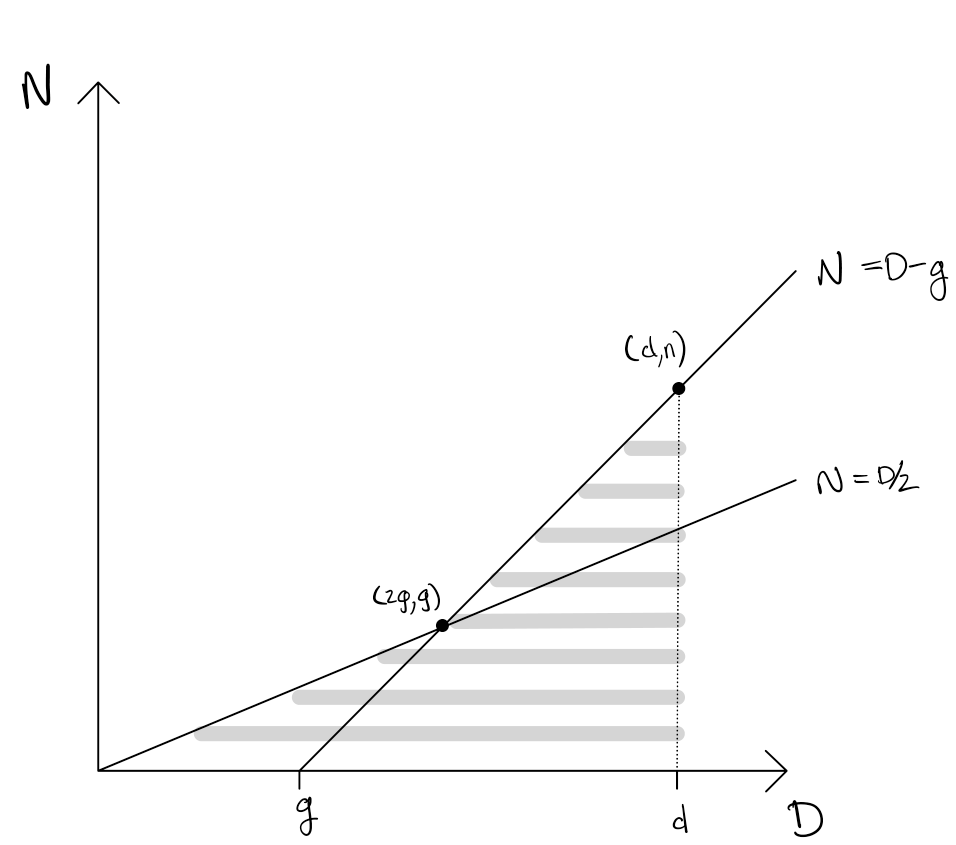
\includegraphics[width=.48\textwidth]{figures/fig-6.8.23.png}
\caption{到 $(d,\allowbreak n)$ 的直线斜率大于到阴影区域任何点的斜率.}\label{src:6.8.23}\end{figure}
对 (b), 选择坐标使单参数子群权满足 $\lambda_0\geq\cdots\geq\lambda_n=0$. 子空间 $\langle x_k,\allowbreak \ldots,\allowbreak x_n\rangle$ 定义超平面 $L_k=V(x_k,\allowbreak \ldots,\allowbreak x_n)$, 诱导到 $\mathbb P^{n-k}$ 的线性投影; $I_k$ 由这些坐标生成. 线性稳定性给出 $e_{\mathcal O_C(1)}(I_k)<(k/n)\deg C$. 命题~\bookref{6.8.19} 给出
\[
\begin{aligned}
e(C,\lambda)&\leq\sum_{k=0}^{n-1}(\lambda_k-\lambda_{k+1})\bigl(e_{\mathcal O_C(1)}(I_k)+e_{\mathcal O_C(1)}(I_{k+1})\bigr)\\
&<\frac{2\deg C}n\sum_{k=0}^{n-1}(\lambda_k-\lambda_{k+1})(k+\tfrac12)\\
&=\frac{2\deg C}n(\tfrac12\lambda_0+\lambda_1+\cdots+\lambda_{n-1}+\tfrac12\lambda_n)\\
&=\frac{2\deg C}n\Bigl(\sum_i\lambda_i-\tfrac12(\lambda_0+\lambda_n)\Bigr)\\
&\leq\frac{2\deg C}n\Bigl(\sum_i\lambda_i-\frac1{n+1}\sum_i\lambda_i\Bigr)
=\frac{2\deg C}{n+1}\sum_i\lambda_i.
\end{aligned}
\]
由 Chow 稳定性判据 (\bookref{6.8.17}) 得 Chow 稳定, 再由命题~\bookref{6.8.18} 得渐近 Hilbert 稳定.
\end{proof}
因此可推出光滑曲线的多重典范嵌入 Chow 稳定.
\begin{proof}[定理~\bookref{6.8.5}(1) 的证明]
嵌入 $|\omega_C^{\otimes k}|$ 的次数为 $d=2k(g-1)$, $N_k+1=(2k+1)(g-1)$. 若 $k\geq5$ (其实 $k\geq3$ 即可), 则 $d>2g$, 定理~\bookref{6.8.22} 给出 Chow 稳定和渐近 Hilbert 稳定. 进一步可找出充分大的 $m$, 使每条此类光滑曲线 $m$-Hilbert 稳定; 见~\cite[定理 1.0.0]{Gie82}.
\end{proof}
\begin{exercise}\label{src:6.8.24}
证明含结点的曲线 $C\subseteq\mathbb P^n$ 不线性稳定.
\end{exercise}
\begin{remark}\label{src:6.8.25}
有光滑曲面不 Chow 稳定, 例如映射 $\mathbb P^2\to\mathbb P^4$, $[x:y:z]\mapsto[xz:yz:x^2:xy:y^2]$ 的像定义的 Steiner 曲面~\cite[例 3.6]{Mor80}.
\end{remark}
\subsection{使非结点曲线去稳定化}\label{src:6.8.5-subsection}
\begin{proposition}\label{src:6.8.26}
设 $C\subseteq\mathbb P^n$ 一般约化, $\deg C/(n+1)<8/7$. 若 $C$ Chow 半稳定, 则不含于超平面, 且至多具有结点奇点.
\end{proposition}
\begin{proof}
若 $C\subseteq H$, 取坐标使 $H=V(x_0)$. 令 $\lambda(t)=\operatorname{diag}(t^{-n},\allowbreak t,\allowbreak \ldots,\allowbreak t)$, 指数严格为正, 所以非半稳定.

若 $p$ 为重数至少 $3$ 的奇点, 取 $p=(1,\allowbreak 0,\allowbreak \ldots,\allowbreak 0)$, $\lambda(t)=(t,\allowbreak 1,\allowbreak \ldots,\allowbreak 1)$. $J_\lambda=(tx_0,\allowbreak x_1,\allowbreak \ldots,\allowbreak x_n)$ 是 $(0,\allowbreak p)$ 的极大理想, 且
\[
e(C,\lambda)=\operatorname{mult}_{(0,p)}(\mathbb A^1\times C)
=\operatorname{mult}_p C\geq3>\frac{16}7\sum_i\lambda_i
>\frac{2\deg C}{n+1}\sum_i\lambda_i.
\]
由判据非半稳定.

若 $p$ 是非结点的二重点, 令 $L\subseteq\mathcal O_C$ 定义 $p$ 处的约化切线. 则 $\mathfrak m_p^2\subsetneq\mathfrak m_p^2+L\subsetneq\mathfrak m_p$, 且 $\dim_k\mathfrak m_p/\mathfrak m_p^2=2$. 取坐标使 (i) $x_0(p)\ne0$, (ii) $v=x_1/x_0$, $u=x_2/x_0$ 张成该商, (iii) $u\in L$, $u^2\in\mathfrak m_p^3$, (iv) $x_3/x_0,\allowbreak \ldots,\allowbreak x_n/x_0\in\mathfrak m_p^2$. 置 $\lambda(t)=\operatorname{diag}(t^4,\allowbreak t^2,\allowbreak t,\allowbreak 1,\allowbreak \ldots,\allowbreak 1)$, 则 $J_\lambda$ 定义支撑在 $(0,\allowbreak p)$ 的闭子概形. 所以 $e(C,\allowbreak \lambda)=e(J_\lambda)$ 是 Hilbert--Samuel 重数, 无论用 $\mathcal O_{\mathbb A^1}\boxtimes\mathcal O_C(1)$ 还是结构层计算均相同. 置 $J_0=(t^4,\allowbreak t^2v,\allowbreak tu,\allowbreak \mathfrak m_p^2)$, 则 $J_\lambda\subseteq J_0$, $e(J_\lambda)\geq e(J_0)$. 令 $J_1=(t^4,\allowbreak \mathfrak m_p^2)$. 因为
\[
(t^2v)^2=t^4v^2\in J_1^2,\qquad
(tu)^4=t^4(u^2)^2\in t^4(\mathfrak m_p^3)^2\subseteq J_1^4,
\]
对 $m\gg0$, $J_0^m=J_1^m$, 所以 $e(J_0)=e(J_1)$. 因而
\[
\begin{aligned}
e(C,\lambda)&=e(J_\lambda)\geq e(J_0)=e(J_1)
=4\cdot2\cdot\operatorname{mult}_p C=16\\
&=\frac{16}7\sum_i\lambda_i>\frac{2\deg C}{n+1}\sum_i\lambda_i.
\end{aligned}
\]
再次由判据得非半稳定. 另见~\cite[命题 3.1]{Mum77} 和~\cite[命题 1.0.4]{Gie82}.
\end{proof}
\begin{remark}\label{src:6.8.27}
有些低次数 Chow 稳定曲线具有比结点更严重的奇点, 但以更高次数重新嵌入后会非半稳定. 例如有次数 $4$ 的 Chow 稳定尖点曲线 $C\subseteq\mathbb P^2$ (见习题~\bookref{8.5.4}), 以次数 $8$ 的线丛 $\mathcal O_C(2)$ 重新嵌入后却非半稳定.
\end{remark}
\begin{proof}[定理~\bookref{6.8.5}(2) 的证明]
若 $C$ 为 $k\geq5$ 的多重典范嵌入稳定曲线, 则
\[
\frac{\deg C}{n+1}=\frac{2k(g-1)}{(2k-1)(g-1)}=\frac{2k}{2k-1}<\frac87.
\]
故命题~\bookref{6.8.26} 保证一般约化且 Chow 半稳定的 $C$ 不含于超平面, 至多具有结点奇点. 要进一步排除非一般约化或非 $k$-多重典范嵌入的曲线, 需相当长而细致的去稳定化分析; 细节见~\cite[\S5]{Mum77}, \cite[\S1]{Gie82} 和~\cite[定理 4.45]{HM98}.
\end{proof}

% Source printed pp. 293-301 / PDF pp. 301-309.
\section{依 Kollár 方法证明射影性}\label{src:6.9}
\begin{epigraph}
然而, 你也许对熟悉的旧有簇仍怀有感情. 尤其看来, \underline{射影}簇在代数几何中发挥着如此核心的技术作用, 即使你想摆脱它们, 实际上也可能办不到. 无论如何, 在可能时证明 [这个空间] 是射影簇, 是非常有趣的.
\epigraphauthor{David Mumford~\cite[441 页]{Mum76}}
\end{epigraph}
遵循 Kollár 在~\cite{Kol90} 中提出的方法, 我们给出 $\overline M_{g,\allowbreak n}$ 射影性的第二个证明; 这一方法建立在 Viehweg 的早期思想~\cite{Vie95} 之上. 为介绍证明射影性的总体策略, 先引入一些术语. 设 $\pi:\mathcal U_g\to\overline{\mathcal M}_g$ 为 $\operatorname{Spec}\mathbb Z$ 上的万有族. 对每个整数 $k\geq1$, 定义 $\overline{\mathcal M}_g$ 上的第 $k$ 个多重典范丛为
\[
\pi_*(\omega_{\mathcal U_g/\overline{\mathcal M}_g}^{\otimes k}).
\]
由命题~\bookref{6.3.23}, 它是向量丛, 当 $k=1$ 时秩为 $g$, 当 $k>1$ 时秩为 $(2k-1)(g-1)$. 其行列式
\[
\lambda_k:=\det\pi_*(\omega_{\mathcal U_g/\overline{\mathcal M}_g}^{\otimes k})
\]
是 $\overline{\mathcal M}_g$ 上的线丛. 当 $k=1$ 时, 它是定义~\bookref{6.10.1} 中的 Hodge 线丛.

\noindent\textbf{证明射影性的策略:} 证明当 $k\gg0$ 时, $\lambda_k$ 的某个正幂下降为粗模空间 $\overline M_g$ 上的丰沛线丛.
\subsection{Kollár 判据与稳定曲线粗模空间的射影性}\label{src:6.9.1-subsection}
Kollár 的策略是利用多重典范丛上的乘法映射
\begin{equation}\label{src:6.9.1}
W:=\operatorname{Sym}^m\underbrace{\pi_*(\omega_{\mathcal U_g/\overline{\mathcal M}_g}^{\otimes k})}_{V}
\longrightarrow\pi_*(\omega_{\mathcal U_g/\overline{\mathcal M}_g}^{\otimes mk})=:Q.
\end{equation}
它依赖与 Hilbert 概形的 GIT 构造完全相同的两个整数 $k,\allowbreak m$. 在稳定曲线 $C\in\mathcal M_g(k)$ 上, 此乘法映射的纤维为
\[
\operatorname{Sym}^m\mathrm H^0(C,\omega_C^{\otimes k})\longrightarrow\mathrm H^0(C,\omega_C^{\otimes mk}),
\]
其核由切出 $|\omega_C^{\otimes k}|:C\to\mathbb P(\mathrm H^0(C,\allowbreak \omega_C^{\otimes k}))$ 的像的 $m$ 次方程组成. 若 $k\geq3$, 则 $\omega_C^{\otimes k}$ 甚丰沛, 且当 $m\gg0$ 时, 可从乘法映射~\bookeqref{6.9.1} 的核恢复 $C$, 因而该乘法映射满射. 令 $w=\operatorname{rk}W$, $q=\operatorname{rk}Q$, $v=\operatorname{rk}V$. 因为 $W$ 表为对称积 $\operatorname{Sym}^mV$, 它具有沿 $\operatorname{GL}_v\to\operatorname{GL}_w$ 的结构群约化 (见定义~\bookref{B.1.64}).

对稳定曲线 $C$, 固定一个基 $\mathrm H^0(C,\allowbreak \omega_C^{\otimes k})\cong k^v$, 得到商
\[
(\operatorname{Sym}^mk^v\twoheadrightarrow\mathrm H^0(C,\omega_C^{\otimes mk}))\in\operatorname{Gr}(q,\operatorname{Sym}^mk^v).
\]
改变基的选择, 只会使这个商相差一个 $\operatorname{PGL}_v$ 作用. 此构造推广到稳定曲线族, 定义一个代数叠态射, 称为\newterm{分类映射}{classifying map}:
\[
\begin{aligned}
\overline{\mathcal M}_g&\longrightarrow[\operatorname{Gr}(q,\operatorname{Sym}^mk^v)/\operatorname{PGL}_v],\\
[C]&\longmapsto[\operatorname{Sym}^mk^v\cong\operatorname{Sym}^m\mathrm H^0(C,\omega_C^{\otimes k})\longrightarrow\mathrm H^0(C,\omega_C^{\otimes mk})].
\end{aligned}
\]
核心思想是借助 $\operatorname{Gr}(q,\allowbreak \operatorname{Sym}^mk^v)$ 的射影性证明 $\overline M_g$ 射影. 为此需要两个性质: 分类映射拟有限, 以及多重典范丛 $V=\pi_*(\omega_{\mathcal U_g/\overline{\mathcal M}_g}^{\otimes k})$ 数值有效.
\begin{theorem}[Kollár 丰沛性判据]\label{src:6.9.2}
设 $X$ 为域 $k$ 上的固有代数空间. 设 $W=\operatorname{Sym}^mV\twoheadrightarrow Q$ 为向量丛满射, 其中 $w=\operatorname{rk}W$, $q=\operatorname{rk}Q$, $v=\operatorname{rk}V$. 假设
\begin{enumerate}[(a)]
\item 分类映射
\[
\begin{aligned}
X&\longrightarrow[\operatorname{Gr}(q,\operatorname{Sym}^mk^v)/\operatorname{PGL}_v],\\
x&\longmapsto[W\otimes\kappa(x)\twoheadrightarrow Q\otimes\kappa(x)]
\end{aligned}
\]
拟有限;
\item $V$ 数值有效.
\end{enumerate}
则 $\det Q$ 丰沛.
\end{theorem}
我们将在~\bookref{6.9.3-subsection} 节详述这些假设并证明判据, 但先说明它如何推出 $\overline M_{g,\allowbreak n}$ 的射影性.
\begin{theorem}[\texorpdfstring{$\overline M_g$}{稳定曲线粗模空间}的射影性]\label{src:6.9.3}
当 $g\geq2$ 且 $N$ 充分可除时, $\overline{\mathcal M}_g$ 上的线丛 $\lambda_{18g-18}^{\otimes N}$ 下降为 $\overline M_g$ 上的线丛, 相对于 $\operatorname{Spec}\mathbb Z$ 丰沛. 特别地, $\overline M_g$ 在 $\operatorname{Spec}\mathbb Z$ 上射影.
\end{theorem}
\begin{proof}
由稳定曲线模叠的固有性 (\bookref{6.5.23}), $\overline{\mathcal M}_g$ 是 $\operatorname{Spec}\mathbb Z$ 上的固有 Deligne--Mumford 叠, 粗模空间 $\overline M_g$ 是 $\operatorname{Spec}\mathbb Z$ 上的固有代数空间. 由习题~\bookref{5.4.29}, 当 $N$ 充分可除时, $\lambda_{18g-18}^{\otimes N}$ 下降为 $\overline M_g$ 上的线丛 $L$. 因丰沛性是开性质 (\bookref{5.6.17}), 只需证明 $\overline M_g$ 定义于域 $k$ 上的情形. 由命题~\bookref{6.3.23}, $\omega_{\mathcal U_g/\overline{\mathcal M}_g}^{\otimes3}$ 相对甚丰沛, 且其推前是秩为 $5g-5$ 的向量丛. 对亏格 $g$ 的稳定曲线 $C$, 完全线性系 $|\omega_C^{\otimes3}|$ 将 $C$ 嵌入为 $\mathbb P^{5g-6}$ 中次数 $m:=6g-6$ 的曲线. 因为 $C$ 由 $m$ 次方程切出, 乘法映射
\[
W:=\operatorname{Sym}^m\pi_*(\omega_{\mathcal U_g/\overline{\mathcal M}_g}^{\otimes3})\twoheadrightarrow\pi_*(\omega_{\mathcal U_g/\overline{\mathcal M}_g}^{\otimes3m})=:Q
\]
是 $\overline{\mathcal M}_g$ 上的向量丛满射, $W$ 的秩为 $w:=\binom{5g-6+m}{m}$, $Q$ 的秩为 $q:=(6m-1)(g-1)$.

分类映射 $\overline{\mathcal M}_g\to[\operatorname{Gr}(q,\allowbreak k^w)/\operatorname{PGL}_{5g-5}]$ 在 $k$-点上单射, 因乘法映射的核唯一确定稳定曲线. 又因稳定曲线的自同构群 $\operatorname{Aut}(C)$ 等同于 $\operatorname{PGL}_{5g-5}$ 作用下 $[C\subseteq\mathbb P^{5g-6}]\in\operatorname{Hilb}^P(\mathbb P^{5g-6})$ 的稳定子, 乘法映射在自同构群之间诱导同构. 因而分类映射拟有限. $V$ 的数值有效性由定理~\bookref{6.9.21} 建立. 由 Gabber 引理 (\bookref{5.6.1}), 可选概形的有限覆盖 $Z\to\overline{\mathcal M}_g$. 在 $Z$ 上应用 Kollár 判据 (\bookref{6.9.2}), 得到 $\lambda_{18g-18}=\det Q$ 在 $Z$ 上的拉回丰沛. 因此 $L$ 沿有限态射 $Z\to\overline{\mathcal M}_g\to\overline M_g$ 的拉回丰沛, 从而 $L$ 在 $\overline M_g$ 上丰沛 (见习题~\bookref{5.5.23}).
\end{proof}
\begin{remark}\label{src:6.9.4}
事实上, 稳定曲线 $C$ 的三重典范嵌入 $|\omega_C^{\otimes3}|:C\hookrightarrow\mathbb P^{5g-6}$ 射影正规, 且由二次方程定义; 见~\cite[58 页]{Mum70b}. 因而乘法映射
\[
\operatorname{Sym}^2\pi_*(\omega_{\mathcal U_g/\overline{\mathcal M}_g}^{\otimes3})\twoheadrightarrow\pi_*(\omega_{\mathcal U_g/\overline{\mathcal M}_g}^{\otimes6})
\]
满射, 同样的论证表明 $\lambda_6$ 的充分可除张量幂下降为 $\overline M_g$ 上的丰沛线丛.
\end{remark}
\begin{corollary}[\texorpdfstring{$\overline M_{g,\allowbreak n}$}{带标记稳定曲线粗模空间}的射影性]\label{src:6.9.5}
对满足 $2g-2+n>0$ 的整数 $g,\allowbreak n$, $\overline M_{g,\allowbreak n}$ 在 $\operatorname{Spec}\mathbb Z$ 上射影.
\end{corollary}
\begin{proof}
已知 $\overline M_{0,\allowbreak 3}=\operatorname{Spec}\mathbb Z$, $\overline M_{1,\allowbreak 1}=\mathbb P^1$. 由上述定理, 当 $g\geq2$ 时 $\overline M_g$ 也射影. 因 $\overline{\mathcal M}_{g,\allowbreak n+1}\to\overline{\mathcal M}_{g,\allowbreak n}$ 是万有族 (命题~\bookref{6.6.12}), 它是稳定曲线族, 且 $L:=\omega_{\overline{\mathcal M}_{g,\allowbreak n+1}/\overline{\mathcal M}_{g,\allowbreak n}}$ 相对于 $\overline{\mathcal M}_{g,\allowbreak n}$ 丰沛 (命题~\bookref{6.3.23}). 因而 $L$ 的某个幂下降为 $\overline M_{g,\allowbreak n+1}$ 上相对于 $\overline M_{g,\allowbreak n}$ 丰沛的线丛 (习题~\bookref{5.4.29}(2)). 于是 $\overline M_{g,\allowbreak n+1}\to\overline M_{g,\allowbreak n}$ 为射影态射, 归纳得到当 $2g-2+n>0$ 时 $\overline M_{g,\allowbreak n}$ 射影.
\end{proof}
\begin{remark}\label{src:6.9.6}
另一种证明 $\overline M_{g,\allowbreak n}$ 射影的方法是, 先证明 $\pi_*(L^{\otimes3})$ 数值有效, 再应用 Kollár 判据 (\bookref{6.9.2}); 其中 $L:=\omega_{\mathcal U_{g,\allowbreak n}/\overline{\mathcal M}_{g,\allowbreak n}}(\sigma_1+\cdots+\sigma_n)$, $\sigma_1,\allowbreak \ldots,\allowbreak \sigma_n$ 是万有族的截面; 见~\cite[命题 4.7]{Kol90}.
\end{remark}
近年来, Kollár 判据已用于越来越一般的情形, 例如 Hassett 的加权带标记曲线模空间~\cite{Has03}, 任意维数的稳定簇的模空间~\cite{KP17}, 以及 K-多重稳定 Fano 簇的模空间~\cite{CP21a,XZ20a}.

\noindent\textbf{本节纲要.} 在~\bookref{6.9.2-subsection} 节讨论代数空间的丰沛性判据, 在~\bookref{6.9.3-subsection} 节证明 Kollár 丰沛性判据, 在~\bookref{6.9.4-subsection} 节建立多重典范丛的数值有效性.
\subsection{正性与丰沛性判据}\label{src:6.9.2-subsection}
将~\bookref{B.2.2-subsection} 节引入的线丛正性概念由概形推广到代数空间, 并将~\bookref{B.2.4-subsection} 节的数值有效向量丛概念推广到代数空间.
\begin{definition}\label{src:6.9.7}
拟紧代数叠 $\mathcal X$ 上的线丛 $L$ 称为:
\begin{enumerate}[(1)]
\item \newterm{无基点}{base point free}的, 若对每个 $x\in|\mathcal X|$, 存在 $s\in\Gamma(\mathcal X,\allowbreak L)$ 使 $s(x)\ne0$;
\item \newterm{半丰沛}{semiample}的, 若某个 $n>0$ 使 $L^{\otimes n}$ 无基点.
\end{enumerate}
域 $k$ 上固有代数空间 $X$ 上的线丛 $L$ 称为:
\begin{enumerate}[(1)]\setcounter{enumi}{2}
\item 丰沛的, 若 $X$ 是概形, 且 $L$ 在通常意义下丰沛 (见命题~\bookref{B.2.8});
\item 数值有效的 (分别地, 严格数值有效的), 若对每条整闭曲线\footnote{由定理~\bookref{5.5.32}, 每条这样的整闭曲线都是射影概形.} $C\subseteq X$, 有 $L\cdot C=\deg L|_C\geq0$ (分别地, $>0$);
\item 大的, 若存在常数 $C$, 对所有 $m\geq0$ 均有 $\mathrm h^0(Z,\allowbreak L|_Z^{\otimes m})\geq Cm^{\dim Z}$.
\end{enumerate}
固有代数空间 $X$ 上的向量丛 $E$ 称为数值有效的, 若 $\mathbb P(E)$ 上的 $\mathcal O_{\mathbb P(E)}(1)$ 数值有效.
\end{definition}
若 $f:X'\to\allowbreak X$ 是代数空间的有限满射, 则 $X$ 上的线丛 $L$ 丰沛当且仅当 $f^*L$ 丰沛 (习题~\bookref{5.5.23}).
\begin{lemma}\label{src:6.9.8}
设 $X$ 为域 $k$ 上的固有代数空间.
\begin{enumerate}[(1)]
\item 若 $f:X'\to\allowbreak X$ 是代数空间的固有满射, 则向量丛 $E$ 数值有效当且仅当 $f^*E$ 数值有效.
\item 若向量丛 $E$ 数值有效, 则 $\det E$ 也数值有效.
\item 若 $f:X'\to\allowbreak X$ 是整代数空间的泛拟有限固有态射, 则线丛 $L$ 为大线丛当且仅当 $f^*L$ 为大线丛.
\end{enumerate}
\end{lemma}
\begin{proof}
(1) 只需对线丛 $L$ 证明. 对像为 $C\subseteq X$ 的整子曲线 $C'\subseteq X'$, 由等式 $\deg(f^*L)|_{C'}=\deg(C'\to\allowbreak C)\deg L|_C$ 即得. 对 (2), 应用 Gabber 引理 (\bookref{5.6.1}), 得到概形的有限覆盖 $f:X'\to\allowbreak X$. 由 (1), 只需证明 $f^*\det E=\det(f^*E)$ 数值有效, 而这由概形的情形 (命题~\bookref{B.2.15}) 得到. (3) 可用与概形情形 (命题~\bookref{B.2.24}) 相同的论证证明.
\end{proof}
下题推广引理~\bookref{B.2.26}; 虽然这里不应用它, 它能帮助理解我们的丰沛性证明策略.
\begin{exercise}[容易]\label{src:6.9.9}
设 $\mathcal X$ 为域 $k$ 上的固有 Deligne--Mumford 叠, 粗模空间为 $\mathcal X\to\allowbreak X$. 若 $\mathcal X$ 上的线丛 $L$ 半丰沛且严格数值有效, 则某个 $N>0$ 使 $L^{\otimes N}$ 下降为 $X$ 上的丰沛线丛, 且 $X$ 射影.
\end{exercise}
上述习题的半丰沛性假设在实际中可能很难验证. GIT 方法将半丰沛性直接纳入半稳定性定义 (定义~\bookref{8.2.1}): 给定约化群 $G$ 在射影空间 $\mathbb P(V)$ 上的线性作用, $0\ne v\in V$ 半稳定当且仅当存在 $d>0$ 及 $s\in\Gamma([\mathbb P(V)/G],\allowbreak \mathcal O(d))$ 使 $s(v)\ne0$. 换言之, 半稳定轨迹 $\mathbb P(V)^{\mathrm{ss}}$ 是最大的开子概形, 使 $\mathcal O(1)$ 在 $[(\mathbb P(V)\setminus\mathbb P(V)^{\mathrm{ss}})/G]$ 上半丰沛; 即 $[\mathbb P(V)^{\mathrm{ss}}/G]$ 是 $[\mathbb P(V)/G]$ 上 $\mathcal O(1)$ 的稳定基点轨迹. Hilbert--Mumford 判据 (\bookref{8.4.4}) 提供了验证半稳定性的有效方法.

概形 $X$ 的 Nakai--Moishezon 丰沛性判据 (\bookref{B.2.28}) 从线丛 $L=\mathcal O_X(D)$ 的数值有效性, 及对每个整闭子概形 $Z$ 存在 $L|_Z^{\otimes N}$ 的截面, 得到半丰沛性. 它对代数空间也成立.
\begin{theorem}[Nakai--Moishezon 丰沛性判据]\label{src:6.9.10}
设 $X$ 为代数闭域 $k$ 上的固有代数空间, $L$ 为 $X$ 上的线丛. 以下条件等价:
\begin{enumerate}[(1)]
\item $L$ 丰沛;
\item $L$ 数值有效, 且对每个整闭子概形 $Z\subseteq X$, $L|_Z$ 为大线丛;
\item $L$ 严格数值有效, 且对每个整闭子概形 $Z\subseteq X$, 存在 $m>0$ 使 $L|_Z^{\otimes m}$ 有效.
\end{enumerate}
\end{theorem}
\begin{proof}
与概形情形 (定理~\bookref{B.2.28}) 相同的论证证明非平凡的方向 (3) $\Rightarrow$ (1).
\end{proof}
\begin{remark}[经典表述]\label{src:6.9.11}
不难将交数的定义推广到代数空间. 即证明 $\chi(Z,\allowbreak L|_Z^{\otimes m})$ 是有理多项式, 并将 $c_1(L)^{\dim Z}\cdot Z$ 定义为 $m^{\dim Z}$ 的归一化系数; 见~\cite[标签 0DN3]{SP}. 对数值有效线丛 $L$, 当 $m\gg0$ 时有 $\chi(Z,\allowbreak L|_Z^{\otimes m})=\mathrm h^0(Z,\allowbreak L|_Z^{\otimes m})$, 因而 $L$ 为大线丛等价于 $c_1(L)^{\dim Z}\cdot Z>0$. 这给出代数空间 $X$ 的 Nakai--Moishezon 判据的经典表述:
\[
L\text{ 丰沛}\quad\Longleftrightarrow\quad c_1(L)^{\dim Z}\cdot Z>0\text{ 对每个整闭子空间 }Z\subseteq X.
\]
Seshadri 判据 (\bookref{B.2.30}) 对固有代数空间成立~\cite{Cor93}, 而 Kleiman 判据 (\bookref{B.2.29}) 对一般固有代数空间 (甚至一般固有概形) 尚不清楚.
\end{remark}
\subsection{Kollár 丰沛性判据的证明}\label{src:6.9.3-subsection}
我们讨论并证明 Kollár 判据 (\bookref{6.9.2}): 若 $X$ 为域 $k$ 上的固有代数空间, $W=\operatorname{Sym}^mV\twoheadrightarrow Q$ 为向量丛满射, $w=\operatorname{rk}W$, $q=\operatorname{rk}Q$, $v=\operatorname{rk}V$, 分类映射
\[
X\longrightarrow[\operatorname{Gr}(q,\operatorname{Sym}^mk^v)/\operatorname{PGL}_v],\qquad x\longmapsto[W\otimes\kappa(x)\twoheadrightarrow Q\otimes\kappa(x)]
\]
拟有限, 且 $V$ 数值有效, 则 $\det Q$ 丰沛.
\begin{remark}[更一般的表述]\label{src:6.9.12}
给出另一种表述, 它不仅更一般, 也提示证明的思路. 设 $W\twoheadrightarrow Q$ 为 $X$ 上秩分别为 $w,\allowbreak q$ 的向量丛满射, 满足:
\begin{enumerate}[(a)]
\item $W$ 具有沿仿射代数群 $G$ 的同态 $G\to\operatorname{GL}_w$ 的结构群约化, 且 $G$ 的像在 $w\times w$ 矩阵的射影空间 $\mathbb P(\operatorname{Mat}_{w,\allowbreak w})$ 中的闭包正规;
\item $W$ 数值有效;
\item 分类映射 $X\to[\operatorname{Gr}(q,\allowbreak W)/G]$ 拟有限;
\item 或者 $G$ 线性约化 (如 $\operatorname{char}k=0$ 且 $G$ 约化), 或者 $G=\operatorname{GL}_{v_1}\times\cdots\times\operatorname{GL}_{v_d}$, 且 $G\to\operatorname{GL}_w$ 为半正表示, 即延拓为映射 $\operatorname{Mat}_{v_1,\allowbreak v_1}\times\cdots\times\operatorname{Mat}_{v_d,\allowbreak v_d}\to\operatorname{Mat}_{w,\allowbreak w}$.
\end{enumerate}
则 $\det Q$ 丰沛~\cite[命题 3.6, 引理 3.9]{Kol90}. Kollár 判据从 $\operatorname{Gr}(q,\allowbreak W)$ 上 Plücker 线丛的丰沛性推出 $\det Q$ 丰沛, 推广了在 $\operatorname{Gr}(q,\allowbreak W)$ 上拟有限的固有概形射影这一事实. 的确, 若 $W$ 为平凡向量丛, 结构群可约化为平凡群 $G=\{1\}$, 分类映射 $X\to\operatorname{Gr}(q,\allowbreak W)$ 拟有限便意味着有限, 从而 Plücker 线丛的拉回 $\det Q$ 丰沛. 证明的核心思想是平凡化 $W$, 实质上归约到这一情形.
\end{remark}
\begin{remark}[展开拟有限性条件]\label{src:6.9.13}
由定义~\bookref{4.3.34}, 分类映射 $X\to[\operatorname{Gr}(q,\allowbreak W)/G]$ 拟有限等价于: (i) 对每个代数闭域 $\bar k$, $X(\bar k)\to\operatorname{Gr}(q,\allowbreak W)(\bar k)$ 具有有限纤维; (ii) 对 $x\in X(\bar k)$, 只有有限多个 $G(\bar k)$ 的元素保持 $\ker(\bar k^w\cong W\otimes\bar k\to\allowbreak Q\otimes\bar k)$ 不变.

事实上, 如~\cite[定理 5.1]{KP17} 所观察的, (c) 中分类映射的拟有限性可替换为 $X(k)\to\operatorname{Gr}(q,\allowbreak W)(k)$ 在集合意义下的拟有限性. 令 $\Gamma:X\to\allowbreak X\times[\operatorname{Gr}(q,\allowbreak W)/G]$ 为分类映射的图, 则集合意义下的拟有限性等价于 $\operatorname{im}\Gamma\to[\operatorname{Gr}(q,\allowbreak W)/G]$ 拟有限, 而这足以使下面的证明成立.
\end{remark}
\begin{remark}[稳定性]\label{src:6.9.14}
上述定理不要求 $X$ 的像落在 $\operatorname{Gr}(q,\allowbreak W)$ 的 $G$-稳定轨迹内. 不过, 若确实如此, 则复合 $X\to[\operatorname{Gr}(q,\allowbreak W)^{\mathrm s}/G]\to\operatorname{Gr}(q,\allowbreak W)\mathbin{/\!/}G$ 是固有代数空间的拟有限态射, 因而有限. 所以 $\det Q^{\otimes w}\otimes\det W^{\otimes(-q)}$ 丰沛, 因为它是 $\operatorname{Gr}(q,\allowbreak W)\mathbin{/\!/}G$ 上丰沛线丛的拉回.
\end{remark}
现在证明 Kollár 丰沛性判据~\cite[引理 3.9]{Kol90}. 另见~\cite[定理 5.1]{KP17} 及~\cite{CLM22} 中的精彩阐述. 证明将 $\det Q$ 的丰沛性归约到它的大性; 后者将在命题~\bookref{6.9.15} 中建立.
\begin{proof}[定理~\bookref{6.9.2} 的证明]
由 Nakai--Moishezon 丰沛性判据 (\bookref{6.9.10}), 只需证明 $\det Q$ 数值有效, 且对每个整子空间 $Z\subseteq X$, $\det Q|_Z$ 为大线丛. 因 $W$ 数值有效, 商 $Q$ 也数值有效, 引理~\bookref{6.9.8}(1) 推出 $\det Q$ 数值有效. 若 $Z\subseteq X$ 为整子空间, 则由 Chow 引理 (\bookref{5.6.5}), 存在来自正规射影概形的泛拟有限固有态射 $Z'\to\allowbreak Z$. 考虑在 $Z'$ 上诱导的满射 $W_{Z'}=\operatorname{Sym}^mV_{Z'}\twoheadrightarrow Q_{Z'}$. 分类映射 $Z'\to\allowbreak X\to[\operatorname{Gr}(q,\allowbreak \operatorname{Sym}^mk^v)/\operatorname{PGL}_v]$ 泛拟有限, 且 $V_{Z'}$ 数值有效. 命题~\bookref{6.9.15} 推出 $\det Q_{Z'}$ 为大线丛, 引理~\bookref{6.9.8}(3) 进一步推出 $\det Q$ 为大线丛.
\end{proof}
在 $X$ 射影的假设下, 我们在分类映射泛有限这一较弱假设下建立 $\det Q$ 为大线丛这一较弱结论. 下面的证明利用大性的双有理不变性, 将射影标架丛 $\mathbb P\mathrm{Fr}_W$ 的紧化爆破, 得到到 $\operatorname{Gr}(q,\allowbreak k^w)$ 的态射, 从而构造截面.
\newpage
\begin{proposition}\label{src:6.9.15}
设 $X$ 为域 $k$ 上的正规射影概形. 设 $W=\operatorname{Sym}^mV\twoheadrightarrow Q$ 为向量丛满射, $w=\operatorname{rk}W$, $q=\operatorname{rk}Q$, $v=\operatorname{rk}V$. 假设
\begin{enumerate}[(a)]
\item 分类映射 $X\to[\operatorname{Gr}(q,\allowbreak \operatorname{Sym}^mk^v)/\operatorname{PGL}_v]$ 泛拟有限;
\item $V$ 数值有效.
\end{enumerate}
则 $\det Q$ 为大线丛.
\end{proposition}
\begin{proof}
\textbf{第一步: 平凡化 $V$.} 定义 $X$ 上的相对射影空间
\[
\mathbb P:=\mathbb P(\mathcal Hom_{\mathcal O_X}(V,\mathcal O_X^{\oplus v})),
\]
并令 $\mathbb P\mathrm{Fr}_V\subseteq\mathbb P$ 为自然映射
\begin{equation}\label{src:6.9.16}
\mathcal O_{\mathbb P}^{\oplus v}\longrightarrow V_{\mathbb P}\otimes\mathcal O_{\mathbb P}(1)
\end{equation}
的行列式非零所定义的开子概形. 该映射由万有商 $\mathcal Hom_{\mathcal O_{\mathbb P}}(V_{\mathbb P},\allowbreak \mathcal O_{\mathbb P}^{\oplus w})\to\mathcal O_{\mathbb P}(1)$ 诱导, 其中 $V_{\mathbb P}$ 为 $V$ 沿 $\mathbb P\to\allowbreak X$ 的拉回. 投影 $\mathbb P\mathrm{Fr}_V\to\allowbreak X$ 为主 $\operatorname{PGL}_v$-丛, 事实上正是 $V$ 的射影标架丛 (见习题~\bookref{B.1.57}). 映射~\bookeqref{6.9.16} 在 $\mathbb P\mathrm{Fr}_V$ 上满射, 定义态射 $\mathbb P\mathrm{Fr}_V\to\operatorname{Gr}(q,\allowbreak \operatorname{Sym}^mk^v)$, 置于 Cartesian 图中:
\[
\begin{tikzcd}[column sep=small]
\mathbb P\arrow[dr,"p"']&\mathbb P\mathrm{Fr}_W\arrow[l,hook']\arrow[r]\arrow[d]&\operatorname{Gr}(q,\operatorname{Sym}^mk^v)\arrow[d]\\
&X\arrow[r]\arrow[ur,phantom,"\square" description]&{[\operatorname{Gr}(q,\operatorname{Sym}^mk^v)/\operatorname{PGL}_w]}.
\end{tikzcd}
\]
注意 $\mathbb P\cong\mathbb P((V^\vee)^{\oplus v})$, 故 $p_*\mathcal O_{\mathbb P}(N)$ 等同于 $\operatorname{Sym}^N((V^\vee)^{\oplus v})$. 因 $V$ 数值有效, 数值有效性的性质 (命题~\bookref{B.2.33}(3)) 推出 $(p_*\mathcal O_{\mathbb P}(N))^\vee$ 数值有效. 下面正是在这里使用假设 (b).

\textbf{第二步: 爆破 $\mathbb P$, 将 $\mathbb P\mathrm{Fr}_W\to\operatorname{Gr}(q,\allowbreak \operatorname{Sym}^mk^v)$ 延拓为映射 $\mathbb P'\to\operatorname{Gr}(q,\allowbreak \operatorname{Sym}^mk^v)$.} 若由~\bookeqref{6.9.16} 诱导的复合
\[
\operatorname{Sym}^m\mathcal O_{\mathbb P}^{\oplus v}\longrightarrow\operatorname{Sym}^mV_{\mathbb P}\otimes\mathcal O_{\mathbb P}(m)\longrightarrow Q_{\mathbb P}\otimes\mathcal O_{\mathbb P}(m)
\]
满射, 便不必爆破. 否则取第 $q$ 个外幂, 得到映射 $\bigwedge^q\operatorname{Sym}^m\mathcal O_{\mathbb P}^{\oplus v}\to\det Q_{\mathbb P}\otimes\mathcal O_{\mathbb P}(mq)$. 令 $I$ 为其像子层, 定义 $\pi:\mathbb P'\to\mathbb P$ 为理想层 $I\otimes(\det Q_{\mathbb P})^\vee\otimes\mathcal O_{\mathbb P}(-mq)\subseteq\mathcal O_{\mathbb P}$ 的爆破. 则 $\mathbb P'\to\mathbb P$ 在 $\mathbb P\mathrm{Fr}_W$ 上为同构, 且有映射 $\mathbb P'\to\operatorname{Gr}(q,\allowbreak \operatorname{Sym}^mk^v)$ 延拓 $\mathbb P\mathrm{Fr}_W\to\operatorname{Gr}(q,\allowbreak \operatorname{Sym}^mk^v)$, 得到交换图
\[
\begin{tikzcd}[column sep=small,row sep=large]
E\arrow[d,hook]&H\arrow[d,hook]&L\arrow[d,hook]\\
\mathbb P'\arrow[r,"\pi"']\arrow[rr,bend left=15]&\mathbb P\arrow[r,dashed]\arrow[d,"p"']&\operatorname{Gr}(q,\operatorname{Sym}^mk^v)\arrow[d]\\
&X\arrow[r]&{[\operatorname{Gr}(q,\operatorname{Sym}^mk^v)/\operatorname{PGL}_w]}.
\end{tikzcd}
\]
其中 $E\subseteq\mathbb P'$ 为例外除子, $H\subseteq\mathbb P$ 为超平面类, $L$ 为 $\operatorname{Gr}(q,\allowbreak \operatorname{Sym}^mk^v)$ 上对应于 Plücker 嵌入的丰沛除子. 滥用记号, 也将 $\det Q$ 看作 $X$ 上的除子. 以下标表示除子的拉回, 有公式
\begin{equation}\label{src:6.9.17}
L_{\mathbb P'}=(\det Q)_{\mathbb P'}+mqH_{\mathbb P'}-E.
\end{equation}
\textbf{第三步: 利用泛拟有限性, 对 $X$ 上的丰沛除子 $A$ 及某个 $N>0$, 构造 $\mathcal O_X(m\det Q-A)\otimes\operatorname{Sym}^{Nmq}((V^\vee)^{\oplus v})$ 的截面.} 因 $X\to[\operatorname{Gr}(q,\allowbreak \operatorname{Sym}^mk^v)/\operatorname{PGL}_w]$ 泛拟有限, $\mathbb P'\to\operatorname{Gr}(q,\allowbreak \operatorname{Sym}^mk^v)$ 也泛拟有限. 命题~\bookref{B.2.24} 推出 $L_{\mathbb P'}$ 为大除子. 对每个甚丰沛除子 $A$, 拉回 $A_{\mathbb P'}$ 有效, Kodaira 引理 (\bookref{B.2.20}) 推出存在 $N>0$ 使 $NL_{\mathbb P'}-A_{\mathbb P'}$ 有效. 利用等式~\bookeqref{6.9.17}, 得到线丛的包含
\[
\begin{aligned}
\mathcal O_{\mathbb P'}(NL_{\mathbb P'}-A_{\mathbb P'})
&\cong\mathcal O_{\mathbb P'}(N(\det Q)_{\mathbb P'}+NmqH_{\mathbb P'}-NE-A_{\mathbb P'})\\
&\subseteq\mathcal O_{\mathbb P'}(N(\det Q)_{\mathbb P'}+NmqH_{\mathbb P'}-A_{\mathbb P'})\\
&\cong\pi^*\bigl(p^*\mathcal O_X(N\det Q-A)\otimes\mathcal O_{\mathbb P}(Nmq)\bigr).
\end{aligned}
\]
选取非零截面 $\mathcal O_{\mathbb P'}\to\pi^*(p^*\mathcal O_X(m\det Q-A)\otimes\mathcal O_{\mathbb P}(mq))$. 因 $\mathbb P$ 正规且 $\pi:\mathbb P'\to\mathbb P$ 双有理, $\pi_*\mathcal O_{\mathbb P'}=\mathcal O_{\mathbb P}$. 对所选截面应用 $\pi_*$ 并利用投影公式, 得到非零截面
\[
\mathcal O_{\mathbb P}\longrightarrow p^*\mathcal O_X(N\det Q-A)\otimes\mathcal O_{\mathbb P}(Nmq).
\]
应用 $p_*$, 得到非零截面 $\mathcal O_X\to\mathcal O_X(N\det Q-A)\otimes p_*\mathcal O_{\mathbb P}(Nmq)$, 将它改写为
\begin{equation}\label{src:6.9.18}
(p_*\mathcal O_{\mathbb P}(Nmq))^\vee\longrightarrow\mathcal O_X(N\det Q-A).
\end{equation}
\textbf{第四步: 爆破 $X$ 使~\bookeqref{6.9.18} 满射, 并利用 $V$ 的数值有效性推出 $\det Q$ 为大线丛.} 如前所述, 由命题~\bookref{B.2.33}(3), $V$ 数值有效推出 $(p_*\mathcal O_{\mathbb P}(Nmq))^\vee\cong\operatorname{Sym}^{Nmq}((V^\vee)^{\oplus v})^\vee$ 数值有效. 因而若~\bookeqref{6.9.18} 满射, 则 $N\det Q-A$ 数值有效, 于是 $N\det Q$ 表为数值有效线丛与丰沛线丛之和, 甚至推出 $\det Q$ 丰沛. 否则, 令 $I$ 为~\bookeqref{6.9.18} 的像子层, 爆破理想层 $I\otimes\mathcal O_X(N\det Q-A)^\vee\subseteq\mathcal O_X$, 得到双有理态射 $f:X'\to\allowbreak X$, 例外除子 $E'$, 以及满射
\[
\begin{aligned}
f^*(p_*\mathcal O_{\mathbb P}(Nmq))^\vee&\twoheadrightarrow M,\\
M&:=f^*(\mathcal O_X(N\det Q-A))\otimes\mathcal O_{X'}(-E').
\end{aligned}
\]
因为左方数值有效, $M$ 也数值有效. 这将 $N\det Q_{X'}$ 表为数值有效除子 $M$, 大除子 $A_{X'}$, 有效除子 $E'$ 之和. 由大性的刻画 (\bookref{B.2.21}), $A_{X'}$ 的某个倍数是丰沛除子与有效除子之和. 因而 $\det Q_{X'}$ 的某个倍数是数值有效, 丰沛, 有效除子之和. 数值有效加丰沛仍丰沛, 丰沛加有效为大, 故 $\det Q_{X'}$ 为大线丛. 又因 $X'\to\allowbreak X$ 双有理, $\det Q$ 为大线丛.
\end{proof}
\subsection{多重典范丛的数值有效性}\label{src:6.9.4-subsection}
我们证明 $\overline{\mathcal M}_g$ 上多重典范丛 $\pi_*(\omega_{\mathcal U_g/\overline{\mathcal M}_g}^{\otimes k})$ 的数值有效性: 证明存在负次数线丛商会与 Ekedahl--Mumford 消灭定理矛盾.
\begin{theorem}[Ekedahl--Mumford 消灭定理]\label{src:6.9.19}
设 $X$ 为代数闭域 $k$ 上的极小一般型光滑射影曲面. 若 $n\geq1$, 则 $\mathrm h^1(X,\allowbreak K_X^{\otimes(-n)})\leq1$. 若 $n>1$ 或 $\operatorname{char}k\ne2$, 则 $\mathrm h^1(X,\allowbreak K_X^{\otimes(-n)})=0$.
\end{theorem}
\begin{proof}
特征 $0$ 的版本是~\cite[定理 2]{Mum67}, 正特征情形是~\cite{Eke88} 的主定理.
\end{proof}
\begin{corollary}\label{src:6.9.20}
设 $X$ 为代数闭域 $k$ 上的极小一般型光滑射影曲面. 设 $D$ 为约化有效 Cartier 除子, 每个连通分支的亏格均至少为 $2$. 若 $n\geq2$, 则 $\mathrm h^1(X,\allowbreak K_X^{\otimes n}(D))\leq1$. 若 $n>2$ 或 $\operatorname{char}k\ne2$, 则 $\mathrm h^1(X,\allowbreak K_X^{\otimes n}(D))=0$.
\end{corollary}
\begin{proof}
由短正合列
\[
0\longrightarrow K_X^{\otimes n}\longrightarrow K_X^{\otimes n}(D)\longrightarrow K_X^{\otimes n}(D)|_D\longrightarrow0
\]
及定理~\bookref{6.9.19} 中的不等式, 只需证明当 $n\geq2$ 时 $\mathrm h^1(X,\allowbreak K_X^{\otimes n}(D)|_D)=0$. 由伴随公式, $K_X^{\otimes n}(D)|_D\cong\omega_D^{\otimes n}$. 因 $D$ 每个连通分支的亏格至少为 $2$, 有 $\mathrm h^1(X,\allowbreak K_X^{\otimes n}(D)|_D)=\mathrm h^1(D,\allowbreak \omega_D^{\otimes n})=0$.
\end{proof}
当 $k\geq2$ 时 $\pi_*(\omega_{\mathcal U_g/\overline{\mathcal M}_g}^{\otimes k})$ 的数值有效性归约为光滑曲线上的稳定曲线族的下述性质.
\begin{theorem}\label{src:6.9.21}
若 $T$ 为域 $k$ 上的光滑连通射影曲线, $\pi:C\to\allowbreak T$ 为稳定曲线族, 则当 $k\geq2$ 时 $\pi_*(\omega_{C/T}^{\otimes k})$ 数值有效.
\end{theorem}
\begin{proof}
\textbf{第一步: 归约到特征 $p$.} 设 $\operatorname{char}k=0$. 因 $T,\allowbreak C$ 在 $k$ 上有限型, 其定义方程只涉及 $k$ 的有限多个系数. 因而存在有限生成 $\mathbb Z$-子代数 $A\subseteq k$ 及 Cartesian 图
\[
\begin{tikzcd}
C\arrow[r]\arrow[d]&\widetilde C\arrow[d]\\
T\arrow[r]\arrow[d]\arrow[ur,phantom,"\square" description]&\widetilde T\arrow[d]\\
\operatorname{Spec}k\arrow[r]\arrow[ur,phantom,"\square" description]&\operatorname{Spec}A.
\end{tikzcd}
\]
其中 $\widetilde C,\allowbreak \widetilde T$ 为 $A$ 上有限型概形. 由极限方法 (\bookref{B.3.7} 与~\bookref{6.2.25}), 还可使 $\widetilde T\to\operatorname{Spec}A$ 为光滑曲线族, $\widetilde C\to\widetilde T$ 为稳定曲线族. 最后, 沿映射 $\operatorname{Spec}R\to\operatorname{Spec}A$ 限制, 可设 $A$ 为离散赋值环, 闭点与泛点的特征分别为 $p>0$ 与 $0$. 因向量丛的数值有效性在泛化下稳定 (\bookref{B.2.34}), 只需证明 $\operatorname{char}k=p>0$ 的情形.

\textbf{第二步: 进一步归约.} 我们断言还可假设:
\begin{enumerate}[(a)]
\item $\pi:C\to\allowbreak T$ 泛光滑;
\item $T$ 的亏格至少为 $2$;
\item $C$ 为极小一般型光滑曲面.
\end{enumerate}
归约到 (a) 由习题~\bookref{6.9.23} 处理. 对 (b), 取有限覆盖 $g:T'\to\allowbreak T$, 其中 $T'$ 为亏格 $g\geq2$ 的光滑连通曲线, 令 $C':=C\times_TT'$. 由对偶化层的性质,
\[
g^*\pi_*(\omega_{C/T}^{\otimes k})\cong\pi'_*(\omega_{C'/T'}^{\otimes k}).
\]
由引理~\bookref{6.9.8}(1), $\omega_{C'/T'}^{\otimes k}$ 数值有效推出 $\omega_{C/T}^{\otimes k}$ 数值有效. 对 (c), 若 $f:\widetilde C\to\allowbreak C$ 为奇点解消, 则 $f_*(\omega_{\widetilde C/T}^{\otimes k})\cong\omega_{C/T}^{\otimes k}$, 从而可设 $C$ 光滑. 若 $C$ 含光滑有理 $(-1)$-曲线 $E$, 则 $E$ 必在 $C\to\allowbreak T$ 的某条纤维中, 否则存在有限覆盖 $E=\mathbb P^1\to\allowbreak T$, 而 $T$ 的亏格 $g\geq2$. 由 Castelnuovo 收缩定理 (\bookref{B.2.6}), 有收缩 $E$ 的态射 $f:C\to\allowbreak C'$. 因 $f_*\omega_{C/T}^{\otimes k}=\omega_{C'/T}^{\otimes k}$, 且收缩光滑有理 $(-1)$-曲线的过程有限步后终止, 可设 $C$ 极小. 因 $T$ 与 $C\to\allowbreak T$ 的泛纤维均光滑且为一般型, $C$ 也是一般型.

\textbf{第三步: 正特征情形.} 若 $\pi_*(\omega_{C/T}^{\otimes k})$ 不数值有效, 则存在商线丛 $\pi_*(\omega_{C/T}^{\otimes k})\twoheadrightarrow M$, 其中 $d=\deg M<0$. 考虑绝对 Frobenius 态射 $F:C\to\allowbreak C$, $F:T\to\allowbreak T$, 它们置于交换图
\[
\begin{tikzcd}
C\arrow[r,"F"]\arrow[d,"\pi"']&C\arrow[d,"\pi"]\\
T\arrow[r,"F"']&T.
\end{tikzcd}
\]
注意 $F^*\pi_*(\omega_{C/T}^{\otimes k})=\pi_*(\omega_{C/T}^{\otimes k})$. 因 $\deg F^*M=pd$, 可反复应用 Frobenius, 使 $d$ 任意小. 具体地, 可使 $M^\vee\cong\omega_T^{\otimes k}\otimes L$, 其中 $L$ 为 $T$ 上甚丰沛线丛. (归约到特征 $p$ 的全部目的, 正是反复应用 Frobenius 任意降低 $M$ 的次数.)

满射 $\pi_*(\omega_{C/T}^{\otimes k})\twoheadrightarrow M\cong(\omega_T^{\otimes k}\otimes L)^\vee$ 给出 $T$ 上的向量丛满射
\[
\pi_*(\omega_{C/T}^{\otimes k})\otimes\omega_T^{\otimes k}\otimes L\twoheadrightarrow\mathcal O_T.
\]
因 $\dim T=1$, 得到
\begin{equation}\label{src:6.9.22}
\mathrm h^1(T,\pi_*(\omega_{C/T}^{\otimes k})\otimes\omega_T^{\otimes k}\otimes L)\geq\mathrm h^1(T,\mathcal O_T)\geq2.
\end{equation}
为得到矛盾, 考察 $\mathrm h^1(C,\allowbreak \omega_C^{\otimes k}\otimes\pi^*L)$. 由 Leray 谱序列在 $E_2$ 页退化, 它以 $\mathrm h^1(T,\allowbreak \pi_*(\omega_C^{\otimes k}\otimes\pi^*L))$ 为下界. 得到不等式
\[
\begin{aligned}
\mathrm h^1(C,\omega_C^{\otimes k}\otimes\pi^*L)
&\geq\mathrm h^1(T,\pi_*(\omega_C^{\otimes k}\otimes\pi^*L))\\
&=\mathrm h^1(T,\pi_*(\omega_{C/T}^{\otimes k}\otimes\pi^*\omega_T^{\otimes k}\otimes\pi^*L))\\
&=\mathrm h^1(T,\pi_*(\omega_{C/T}^{\otimes k})\otimes\omega_T^{\otimes k}\otimes L)\\
&\geq\mathrm h^1(T,\mathcal O_T)\geq2.
\end{aligned}
\]
第一个等号用 $\omega_C\cong\omega_{C/T}\otimes\pi^*\omega_T$, 第二个等号用投影公式, 最后用~\bookeqref{6.9.22}. 因 $L$ 甚丰沛, 存在由 $\pi:C\to\allowbreak T$ 的光滑纤维的并组成的有效除子 $D$, 使 $\mathcal O_C(D)\cong\pi^*L$. 上述不等式与将推论~\bookref{6.9.20} 应用于 $D$ 所得结论矛盾. 另见~\cite[定理 4.3]{Kol90} 与~\cite[定理 6.10]{CLM22}.
\end{proof}
\begin{exercise}[细节]\label{src:6.9.23}
设 $T$ 为域 $k$ 上的光滑连通射影曲线. 证明: 若每个泛光滑稳定族的 $\pi_*(\omega_{C/T}^{\otimes k})$ 均数值有效, 则每个稳定族的该向量丛均数值有效.
\end{exercise}

% Source printed pp. 302-307 / PDF pp. 310-315.
\section{\texorpdfstring{$\overline M_g$}{稳定曲线粗模空间}的几何一瞥}\label{src:6.10}
\begin{epigraph}
当 [Zariski] 说出``代数簇''时, 他的声音有一种共鸣, 清楚地表明他正凝视一个秘密花园. 我立即也想拥有这种能力\ldots\ 尤其是, 我迷上了这花园中的一种西番莲: Riemann 模空间.
\epigraphauthor{David Mumford~\cite[225 页]{AI97}}
\end{epigraph}
存在性, 不可约性和射影性 (定理~\hyperref[thm:A]{A}) 当然只是研究 $\overline M_g$ 的起点. 现在可以开始提出各种几何问题:
\begin{itemize}
\item 它的丰沛锥或有效锥是什么?
\item 它的 Kodaira 维数或典范模型是什么?
\item 粗模空间有什么奇点?
\item 它的奇异上同调, Chow 上同调或 Hodge 上同调是什么?
\item 对整数 $r,\allowbreak d$, 一般的亏格 $g$ 曲线是否具有一个 $g_d^r$?
\end{itemize}
注意, 甚至要讨论丰沛线丛及其他双有理性质, 都需要 $\overline M_g$ 的射影性. 另一方面, $\overline M_g$ 的不可约性使我们能将一般曲线的性质, 转化为 $\overline M_g$ 中满足该性质的曲线组成非空开轨迹这一命题. 若该性质是开条件, 只需给出一条具有此性质且可光滑化的曲线.

我们不可能给出全面综述; 毕竟, $\overline M_g$ 也许是过去六十年来研究最多的单个簇. 请参阅~\cite{Mum83,ACGH85,HM98,ACG11,FM13}; 这里也作几点简略说明.

\noindent\textbf{重言线丛.}
\begin{definition}[Hodge 线丛 $\lambda$]\label{src:6.10.1}
令 $\pi:\mathcal U_{g,\allowbreak n}\to\overline{\mathcal M}_{g,\allowbreak n}$ 表示万有族. \newterm{Hodge 向量丛}{Hodge vector bundle}定义为推前 $E:=\pi_*(\omega_{\mathcal U_{g,\allowbreak n}/\overline{\mathcal M}_{g,\allowbreak n}})$. 由稳定曲线族的性质 (\bookref{6.3.23}), 它是向量丛. \newterm{Hodge 线丛}{Hodge line bundle}定义为行列式 $\lambda:=\det E$.
\end{definition}
\begin{exercise}\label{src:6.10.2}
证明: 沿每个遗忘态射 (\bookref{6.6.10}) 和粘合态射 (\bookref{6.6.16}), $\lambda$ 的拉回仍为 $\lambda$.
\end{exercise}
更一般地, 对每个整数 $k\geq0$, 可定义线丛
\[
\lambda_k:=\det\pi_*(\omega_{\mathcal U_{g,n}/\overline{\mathcal M}_{g,n}}^{\otimes k}),
\]
当 $k=1$ 时恢复 Hodge 线丛 $\lambda=\lambda_1$. 线丛 $\lambda_k$ 与下列线丛密切相关:
\[
\Lambda_k:=\det\mathrm R\pi_*(\omega_{\mathcal U_{g,n}/\overline{\mathcal M}_{g,n}}^{\otimes k}).
\]
由上同调与基变换 (\bookref{A.6.2}), 此处的导出推前是振幅在 $[0,\allowbreak 1]$ 中的完美复形, 其行列式为
\[
\det\pi_*(\omega_{\mathcal U_{g,n}/\overline{\mathcal M}_{g,n}}^{\otimes k})\otimes\det(\mathrm R^1\pi_*(\omega_{\mathcal U_{g,n}/\overline{\mathcal M}_{g,n}}^{\otimes k}))^\vee.
\]
由 Grothendieck--Serre 对偶, 对 $i=0,\allowbreak 1$ 有 $\mathrm R^i\pi_*\omega_{\mathcal U_{g,\allowbreak n}/\overline{\mathcal M}_{g,\allowbreak n}}\cong\mathrm R^{1-i}\pi_*\mathcal O_{\overline{\mathcal M}_{g,\allowbreak n}}$, 而当 $k\geq2$ 时 $\mathrm R^1\pi_*\omega_{\mathcal U_{g,\allowbreak n}/\overline{\mathcal M}_{g,\allowbreak n}}^{\otimes k}=0$, 故 $\Lambda_0=\Lambda_1=\lambda$, 且当 $k\geq2$ 时 $\Lambda_k=\lambda_k$. 此外, 由一个一般事实 (见~\cite[定理 4]{KM76}), $\overline{\mathcal M}_{g,\allowbreak n}$ 上存在线丛 $M_0,\allowbreak M_1,\allowbreak M_2$, 在加法记号下满足
\begin{equation}\label{src:6.10.3}
\Lambda_k=\binom{k}{2}M_2+kM_1+M_0
\end{equation}
对所有 $k\geq0$ 成立. 代入 $k=0,\allowbreak 1$, 得到 $M_0=\Lambda_0=\lambda$, $M_1=0$. 我们将首项系数 $M_2$ 作为 CM 线丛的定义.
\begin{definition}[CM 线丛]\label{src:6.10.4}
\newterm{Chow--Mumford 线丛}{Chow--Mumford line bundle}, 简称 \newterm{CM 线丛}{CM line bundle} $L_{\mathrm{CM}}$, 定义为展开式~\bookeqref{6.10.3} 的首项系数 $M_2$.
\end{definition}
\begin{remark}[Kappa 类]\label{src:6.10.5}
CM 线丛也称为 \newterm{Kappa 类}{kappa class}, 等价地可定义为
\[
\kappa:=\pi_*\bigl(c_1(\omega_{\mathcal U_{g,n}/\overline{\mathcal M}_{g,n}})^2\bigr)\in\operatorname{CH}^1(\overline{\mathcal M}_{g,n});
\]
Chow 群的定义见~\bookref{7.1.6-subsection} 节. 请注意, 此构造与 $\lambda_2=\det\pi_*(\omega_{\mathcal U_{g,\allowbreak n}}^{\otimes2})$ 很不相同. 这里取 $c_1(\omega_{\mathcal U_{g,\allowbreak n}/\overline{\mathcal M}_{g,\allowbreak n}})\in\operatorname{CH}^1(\overline{\mathcal U}_{g,\allowbreak n})$, 在 $\operatorname{CH}^2(\overline{\mathcal U}_{g,\allowbreak n})$ 中取其自交, 再沿固有可表态射 $\mathcal U_{g,\allowbreak n}\to\overline{\mathcal M}_{g,\allowbreak n}$ 推前到 $\operatorname{CH}^1(\overline{\mathcal M}_{g,\allowbreak n})$. 在等价 $\operatorname{CH}^1(\overline{\mathcal M}_{g,\allowbreak n})\cong\operatorname{Pic}(\overline{\mathcal M}_{g,\allowbreak n})$ 下, $\kappa$ 对应 $L_{\mathrm{CM}}$. 更一般地, 可定义高阶 Kappa 类
\[
\kappa_i:=\pi_*\bigl(c_1(\omega_{\mathcal U_{g,n}/\overline{\mathcal M}_{g,n}})^{i+1}\bigr)\in\operatorname{CH}^i(\overline{\mathcal M}_{g,n}).
\]
\end{remark}
\noindent\textbf{边界除子与 $\Psi$ 类.} 回顾定义~\bookref{6.6.17}, 边界除子 $\delta\subseteq\overline{\mathcal M}_{g,\allowbreak n}$ 为奇异曲线的轨迹. 它是有效 Cartier 除子, 甚至是正规交叉除子 (命题~\bookref{6.6.19}). 边界除子可写为并 $\delta=\delta_0\cup\bigcup_{i,\allowbreak I}\delta_{i,\allowbreak I}$, 其中
\begin{itemize}
\item $\delta_0$ 为不可约奇异曲线轨迹的闭包, 即粘合态射 (\bookref{6.6.16}) $\overline{\mathcal M}_{g-1,\allowbreak n+2}\to\overline{\mathcal M}_{g,\allowbreak n}$ 的像;
\item $\delta_{i,\allowbreak I}$ 为具有亏格 $i$ 的不可约分支且该分支包含由 $I$ 标记的点的曲线轨迹的闭包, 即
\[
\overline{\mathcal M}_{i,I\cup\{p\}}\times\overline{\mathcal M}_{g-i,I^c\cup\{q\}}\longrightarrow\overline{\mathcal M}_{g,n}
\]
的像, 其中 $0\leq i\leq g$, $I\subseteq\{1,\allowbreak \ldots,\allowbreak n\}$, 且来源模叠非空.
\end{itemize}
因 $\delta,\allowbreak \delta_0,\allowbreak \delta_{i,\allowbreak I}$ 均为有效 Cartier 除子, 它们定义线丛
\[
\delta:=\mathcal O_{\overline{\mathcal M}_{g,n}}(\delta),\quad
\delta_0:=\mathcal O_{\overline{\mathcal M}_{g,n}}(\delta_0),\quad
\delta_{i,I}:=\mathcal O_{\overline{\mathcal M}_{g,n}}(\delta_{i,I})
\]
(见习题~\bookref{7.1.19}); 这里滥用同一符号.
\newpage
\begin{definition}[Psi 线丛]\label{src:6.10.6}
设 $\sigma_i:\overline{\mathcal M}_{g,\allowbreak n}\to\mathcal U_{g,\allowbreak n}$ 为万有族的第 $i$ 个截面, $\mathcal I_{\sigma_i}\subseteq\mathcal O_{\mathcal U_{g,\allowbreak n}}$ 为其理想层. 定义 \newterm{Psi 线丛}{Psi line bundle} $\psi_i:=\mathcal I_{\sigma_i}/\mathcal I_{\sigma_i}^2$ 为 $\sigma_i$ 的余法丛, 并用加法记号定义
\[
\psi:=\psi_1+\cdots+\psi_n.
\]
有如下等同:
\[
\psi_i\cong\sigma_i^*\Omega_{\mathcal U_{g,n}/\overline{\mathcal M}_{g,n}}\cong\sigma_i^*\omega_{\mathcal U_{g,n}/\overline{\mathcal M}_{g,n}}\cong\sigma_i^*\mathcal O_{\mathcal U_{g,n}}(-\sigma_i(\overline{\mathcal M}_{g,n})).
\]
Psi 类定义为 $c_1(\psi_i)\in\operatorname{CH}^1(\overline{\mathcal M}_{g,\allowbreak n})$.
\end{definition}
\begin{definition}[典范线丛]\label{src:6.10.7}
在域 $k$ 上, 设 $\Omega_{\overline{\mathcal M}_{g,\allowbreak n}/k}$ 为微分层 (例~\bookref{5.1.3}); 因 $\overline{\mathcal M}_{g,\allowbreak n}$ 光滑, 它是向量丛. 定义典范线丛为
\[
K=K_{\overline{\mathcal M}_{g,n}}:=\det\Omega_{\overline{\mathcal M}_{g,n}/k}.
\]
\end{definition}
\begin{exercise}\label{src:6.10.8}
\begin{enumerate}[(a)]
\item 若 $C$ 是两条光滑曲线 $C_1,\allowbreak C_2$ 沿 $p_1\in C_1$, $p_2\in C_2$ 的结点并 $C_1\cup C_2$, 证明有向量空间的自然等同
\[
\delta\otimes\kappa([C])\cong T_{p_1}C_1\otimes T_{p_2}C_2.
\]
\item 证明 $\delta$ 沿粘合态射 $\overline{\mathcal M}_{g,\allowbreak n+2}\to\overline{\mathcal M}_{g,\allowbreak n}$ 的拉回为 $\delta-\psi_{n+1}-\psi_{n+2}$, 沿 $\overline{\mathcal M}_{g_1,\allowbreak n_1}\times\overline{\mathcal M}_{g_2,\allowbreak n_2}\to\overline{\mathcal M}_{g,\allowbreak n}$ 的拉回为 $(\delta-\psi_{n_1})\boxtimes(\delta-\psi_{n_2})$.
\item 证明 $\delta-\psi$ 与 $K+\psi$ 在沿每个粘合态射拉回时保持不变.
\end{enumerate}
另见~\cite[第 4 节]{Knu83b}, \cite[命题 3.32]{HM98} 与~\cite[第 XVII.4 节]{ACG11}.
\end{exercise}
\begin{exercise}[与粗模空间比较]\label{src:6.10.9}
设 $\Delta_i,\allowbreak \Delta$ 为 $\overline M_g$ 上的线丛, 对应于 $\delta_i,\allowbreak \delta\subseteq\overline{\mathcal M}_g$ 在粗模空间映射 $\pi:\overline{\mathcal M}_g\to\overline M_g$ 下的像. 证明
\[
\begin{aligned}
\pi^*\Delta_i&=\begin{cases}\delta_i&\text{若 }i\ne1,\\2\delta_1&\text{若 }i=1,\end{cases}\\
\pi^*\Delta&=\delta+\delta_1,\\
\pi^*K_{\overline M_g}&=K_{\overline{\mathcal M}_g}-\delta_1.
\end{aligned}
\]
\end{exercise}
\noindent\textbf{Picard 群.} 现在聚焦于无标记稳定曲线模叠 $\overline{\mathcal M}_g$. 上述线丛满足若干关系:
\begin{equation}\label{src:6.10.10}
\begin{aligned}
K&=13\lambda-2\delta,\\
L_{\mathrm{CM}}&=12\lambda-\delta=-\lambda+\lambda_2=\frac{12}{13}\left(K+\frac{11}{12}\delta\right),\\
\lambda_2&=L_{\mathrm{CM}}+\lambda=13\lambda-\delta=K+\delta,\\
\lambda_k&=\binom{k}{2}L_{\mathrm{CM}}+\lambda=(6k^2-6k+1)\lambda-\binom{k}{2}\delta\quad(k\geq2).
\end{aligned}
\end{equation}
公式 $L_{\mathrm{CM}}=12\lambda-\delta$ 和 $K_{\overline{\mathcal M}_g}=13\lambda-2\delta$ 称为 Mumford 公式, 由 Grothendieck--Riemann--Roch 建立; 见~\cite[第 5 节]{Mum83}, \cite[第 3.E 节]{HM98} 与~\cite[第 XIII.7 节]{ACG11}.

这些公式表明, 线丛 $K,\allowbreak \lambda,\allowbreak \delta,\allowbreak L_{\mathrm{CM}},\allowbreak \lambda_k$ 均在同一个二维子空间 $\langle\lambda,\allowbreak \delta\rangle\subseteq\operatorname{Pic}(\overline{\mathcal M}_g)$ 中. 其中的线丛与 $s\lambda-\delta$ 成比例, 有理数 $s$ 称为\newterm{斜率}{slope}. 也可将线丛表为与 $L_{\mathrm{CM}}+s_{\mathrm{CM}}\lambda$ 或 $K+\alpha\delta$ 成比例的形式, 其关系为 $s=12-s_{\mathrm{CM}}=13/(2-\alpha)$.
\newpage
\begin{theorem}\label{src:6.10.11}
在满足 $\operatorname{char}k\ne2$ 的域 $k$ 上,
\[
\operatorname{Pic}(\overline{\mathcal M}_g)\cong\mathbb Z\langle\lambda,\delta_0,\delta_1,\ldots,\delta_{\lfloor g/2\rfloor}\rangle.
\]
特别地, $\operatorname{Pic}(\overline{\mathcal M}_g)_{\mathbb Q}\cong\mathbb Q\langle\lambda,\allowbreak \delta_0,\allowbreak \delta_1,\allowbreak \ldots,\allowbreak \delta_{\lfloor g/2\rfloor}\rangle$.
\end{theorem}
\begin{proof}
Harer~\cite{Har83,Har88} 在 $\mathbb C$ 上用拓扑方法证明了它, Arbarello 与 Cornalba~\cite{AC87} 用代数方法证明了它. \cite{FV23} 将其推广到任意域 (甚至基概形). 粗模空间的结论由如下事实得到: Deligne--Mumford 叠上的每个线丛均有一个正倍数下降到粗模空间 (见命题~\bookref{5.4.27} 与习题~\bookref{5.4.29}).
\end{proof}
\begin{figure}[htbp]
\centering\begin{tikzpicture}
\node[inner sep=0,anchor=south west] (im) at (0,0) {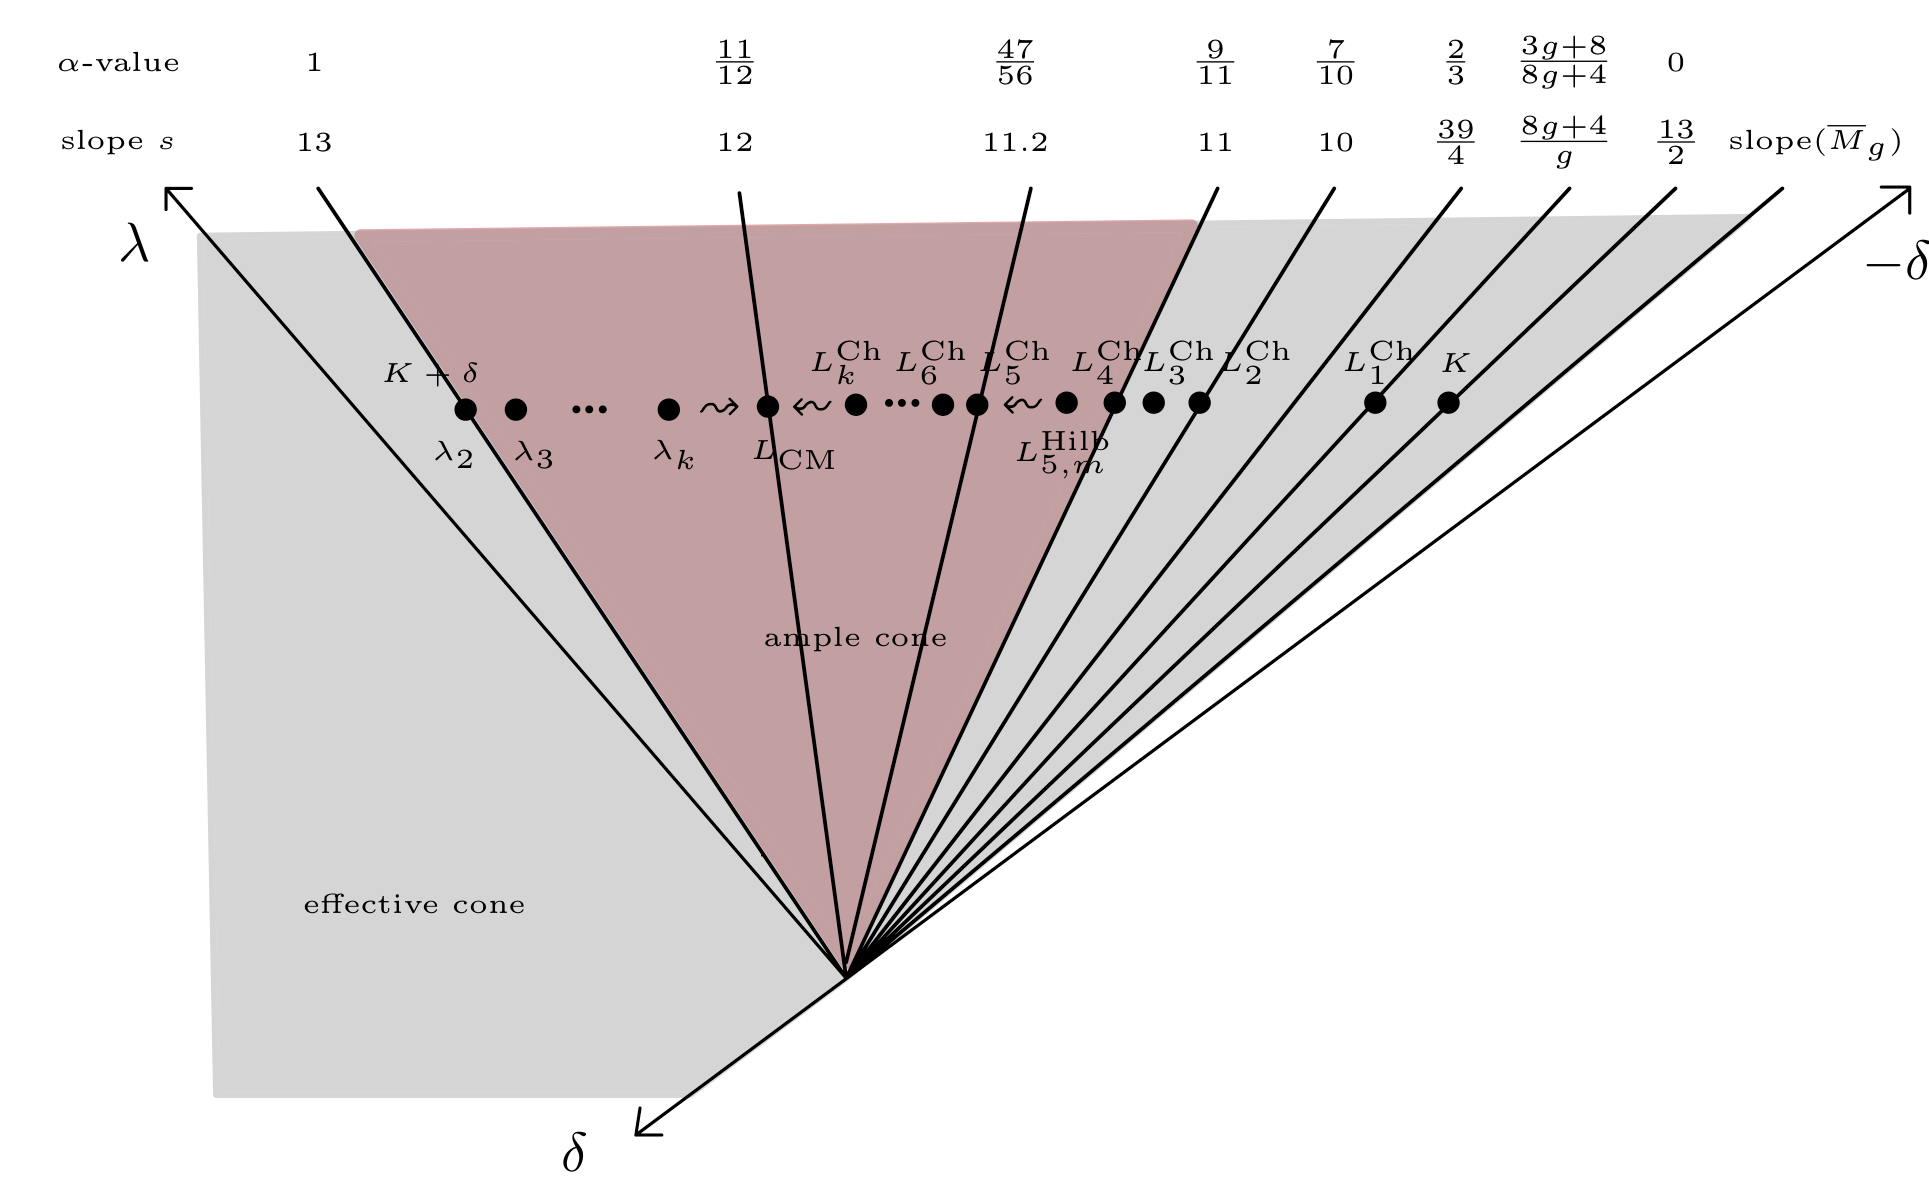
\includegraphics[width=.95\textwidth]{figures/moduli-cones.png}};
\begin{scope}[x={(im.south east)},y={(im.north west)}]
\fill[fill=white] (0.025937,0.964789) rectangle (0.096542,0.929577);
\node[font=\tiny,inner sep=0pt] at (0.061239,0.947183) {$\alpha$ 值};
\fill[fill=white] (0.027378,0.899061) rectangle (0.095101,0.862441);
\node[font=\tiny,inner sep=0pt] at (0.061239,0.880751) {斜率 $s$};
\fill[fill=white] (0.893372,0.899061) rectangle (0.991354,0.859155);
\node[font=\tiny,inner sep=0pt] at (0.942363,0.879108) {斜率 $(\overline M_g)$};
\fill[fill={rgb,255:red,213;green,213;blue,213}] (0.154179,0.252113) rectangle (0.275216,0.219249);
\node[font=\tiny,inner sep=0pt] at (0.214697,0.235681) {有效锥};
\fill[fill={rgb,255:red,194;green,159;blue,161}] (0.392507,0.477934) rectangle (0.494236,0.444601);
\node[font=\tiny,inner sep=0pt] at (0.443372,0.461268) {丰沛锥};
\end{scope}\end{tikzpicture}

\caption{$\lambda\delta$ 平面中的有效锥与丰沛锥}\label{src:6.10.12}
\end{figure}
\noindent\textbf{丰沛锥.} Kollár 判据 (\bookref{6.9.2}) 不仅给出 $\overline M_g$ 射影, 还给出当 $k\geq6$ 时 $\lambda_k$ 丰沛 (见注记~\bookref{6.9.4}). 线丛 $\lambda$ 数值有效; 它定义 Torelli 态射 $\overline M_g\to\overline A_g$. 因而当 $s>12$ 时 $s\lambda-\delta$ 丰沛. 注意关系式~\bookeqref{6.10.10} 蕴含 $L_{\mathrm{CM}}\sim\lim_{k\to\infty}\lambda_k$.

另一方面, GIT 构造对 $k\geq5$, $m\gg0$ 给出丰沛线丛 $L_k^{\mathrm{Ch}}$, $L_{k,\allowbreak m}^{\mathrm{Hilb}}$. 对其他 $k,\allowbreak m$, GIT 构造与 $\overline M_g$ 双有理的射影簇. 这些线丛的类成比例于
\[
\begin{aligned}
L_k^{\mathrm{Ch}}&\sim\begin{cases}(8+\frac4g)\lambda-\delta&\text{若 }k=1,\\(12-\frac4k)\lambda-\delta&\text{若 }k>1,\end{cases}\\
L_{k,m}^{\mathrm{Hilb}}&\sim\begin{cases}
\left(\dfrac{2+(m-1)((8g+4)m-2g+2))}{gm}\right)\lambda-\delta&\text{若 }k=1,\\
\left(\dfrac{12mk^2-4mk-4k+2}{mk^2}\right)\lambda-\delta&\text{若 }k>1;
\end{cases}
\end{aligned}
\]
见~\cite[定理 5.15]{Mum77}, \cite[第 2 节]{CH88} 与~\cite[第 1.5 节]{Vie89}. 固定 $k$, 有 $\lim_{m\to\infty}L_{k,\allowbreak m}^{\mathrm{Hilb}}\sim L_k^{\mathrm{Ch}}$, 而 $\lim_{k\to\infty}L_k^{\mathrm{Ch}}\sim L_{\mathrm{CM}}$. 取 $k=5$, 得到当 $s\geq11.2$ 时 $s\lambda-\delta$ 丰沛. 然而还可得到更强结论! Cornalba 与 Harris 从 GIT 推出的正性出发, 进一步证明 $s\lambda-\delta$ 丰沛当且仅当 $s>11$, 从而确定 $\operatorname{Pic}(\overline M_g)$ 的 $\lambda\delta$ 平面中的丰沛锥~\cite{CH88}. 完整的丰沛锥尚未确定, 但有一个有趣的 $F$-猜想: 它给出有限多个检验曲线, 并断言线丛丰沛当且仅当它与每条检验曲线的交数均为正. 这里不列举这些曲线, 但其中包括 $\overline{\mathcal M}_g$ 中参数化椭圆尾的有理曲线: 固定亏格 $g-1$ 的单标记曲线 $(C,\allowbreak p)$, 改变以结点方式附着的椭圆曲线 $(E,\allowbreak p)$ 的 $j$-不变量.

\noindent\textbf{有效锥与 Kodaira 维数.} 虽然 $\delta$ 显然是有效除子, 但使 $s\lambda-\delta$ 有效的最小 $s$, 即 $\overline M_g$ 的斜率, 并不清楚. 将 $g+1$ 写为 $(r+1)(s+1)$ 且 $s\geq3$, Harris 与 Mumford 定义 Brill--Noether 除子
\[
D_{\mathrm{BN}}:=\overline{\{[C]\mid C\text{ 具有一个 }g_d^r\}}\subseteq\overline{\mathcal M}_g,
\]
其类成比例于 $(g+3)\lambda-\frac{g+1}{6}\delta_0-\sum_{i=1}^{\lfloor g/2\rfloor}i(g-i)\delta_i$, 与 $r,\allowbreak s$ 无关; 见~\cite{HM82} 与~\cite[第 6.F 节]{HM98}. 当 $g$ 为奇数时, $D_{\mathrm{BN}}$ 的斜率为 $6+12/(g+1)$. 当 $g\geq24$ 时, 此斜率小于 $13/2$. 因 $K_{\overline{\mathcal M}_g}=13\lambda-2\delta$, 可推出 $K_{\overline{\mathcal M}_g}$ 位于有效锥的内部, 即下降为 $\overline M_g$ 上的大线丛. Eisenbud 与 Harris 将此推广到所有 $g\geq24$~\cite{EH87}. 因而对 $g\geq24$, $\overline M_g$ 的 Kodaira 维数为 $3g-3$, 且 $\overline M_g$ 为一般型.

这否定了 Severi 关于所有 $g$ 的 $\overline M_g$ 均为单有理的猜想. Severi 曾证明当 $g\leq10$ 时 $\overline M_g$ 单有理 (见~\bookref{1.1.2-subsection} 节), 现在已知对 $g\leq14$ 也成立~\cite{Ver05}. 对 $15$ 至 $23$ 之间的某些亏格, $\overline M_g$ 的 Kodaira 维数仍未知. 一般的 $\overline M_g$ 的斜率也未知. Harris 与 Mumford 曾猜想斜率至少为 $6+12/(g+1)$, 但 Farkas 与 Popa~\cite{FP05} 否定了它. 如今似乎存在不同看法: 有人认为 $\overline M_g$ 的斜率至多为 $6$, 也有人认为它趋于 $0$.

\noindent\textbf{$\overline M_g$ 的双有理几何.} Mumford 在利用 Chow 概形的 GIT 构造 $\overline M_g$ 的同一篇论文~\cite{Mum77} 中观察到, 其他 GIT 设置会给出 $\overline M_g$ 的双有理模型, 参数化奇点可能比结点更差的曲线. 具体地, 在亏格 $3$ 时, 他构造了有理映射
\[
\overline M_3\dashrightarrow\mathbb P(\operatorname{Sym}^4(\mathbb C^3))\mathbin{/\!/}\operatorname{SL}_3,
\]
将具有椭圆尾 (即通过结点附着的亏格 $1$ 曲线) 的曲线收缩为尖点曲线, 将椭圆桥 (即两条亏格 $1$ 曲线沿两点的结点并) 映为挠结点曲线, 并将超椭圆轨迹收缩为一点, 此点对应二重二次曲线.

因 $g\gg0$ 时 $\overline M_g$ 为一般型, 自然会问它的典范模型
\[
\overline M_g^{\mathrm{can}}=\operatorname{Proj}\bigoplus_d\Gamma(\overline{\mathcal M}_g,K_{\overline{\mathcal M}_g}^{\otimes d})
\]
是什么; 由~\cite{BCHM10}, 它是射影簇. $\overline M_g$ 是特别有趣的高维簇, 而其模描述为几何研究提供了切入点, 因而很适合用来检验极小模型纲领的工具. 为回答此问题, Hassett 在~\cite{Has05} 中提出考虑对数典范模型
\begin{equation}\label{src:6.10.13}
\overline M_g(\alpha):=\operatorname{Proj}\bigoplus_{d\geq0}\mathrm H^0(\overline{\mathcal M}_g,\lfloor d(K_{\overline{\mathcal M}_g}+\alpha\delta)\rfloor),
\end{equation}
从 $\overline M_g$ 过渡到 $\overline M_g^{\mathrm{can}}$, 其中 $\delta$ 为边界除子. 注意 $\overline M_g=\overline M_g(1)$ (因 $K+\delta$ 在 $\overline M_g$ 上丰沛), 而 $\overline M_g^{\mathrm{can}}=\overline M_g(0)$. 对任意亏格, Hassett 与 Hyeon 构造首个除子收缩 $\overline M_g\to\overline M_g(9/11)$~\cite{HH09}, 以及首个翻转
\[
\overline M_g(9/11)\longrightarrow\overline M_g(7/10)\longleftarrow\overline M_g(7/10-\epsilon),\qquad\epsilon\ll1
\]
~\cite{HH13}. 引人注目的是, 他们为每个射影簇给出模描述, 并证明首个收缩以尖点奇点替代椭圆尾, 首个翻转以挠结点曲线替代椭圆桥的轨迹.

存在参数化任意维数一般型簇的射影模空间, 因而很自然会把 $\overline M_g$ 看作这种模空间中的一点. Hacking 证明 $\overline{\mathcal M}_g$ 刚性, 即没有非平凡形变, 等价地 $\mathrm H^1(\overline{\mathcal M}_g,\allowbreak T_{\overline{\mathcal M}_g})=0$~\cite{Hac08}. 这印证了 Kapranov 的预期: 若 $X$ 为 $n$ 维光滑簇, 则迭代考虑参数化 $X$ 的形变的模空间 $X[1]$, 参数化 $X[1]$ 的形变的模空间 $X[2]$, 等等, 此过程恰在 $n$ 步后终止.

\noindent\textbf{$\overline M_g$ 的奇点.} 因 $\overline{\mathcal M}_g$ 光滑, 粗模空间的局部结构 (\bookref{5.4.13}) 推出 $\overline M_g$ 具有有限商奇点. Harris 与 Mumford 借助 Reid--Tai 判据证明 $\overline M_g$ 具有典范奇点~\cite{HM82}; 换言之, 多重典范截面延拓到 $\overline M_g$ 的奇点解消上. 这是他们证明 $\overline M_g$ 为一般型所必需的性质.

一般的亏格 $g\geq3$ 光滑曲线 $C\in\mathcal M_g(k)$ 具有平凡自同构群. 因 $\mathcal M_g$ 不可约, 只需给出一条自同构群平凡的光滑曲线便可推出此结论. 它意味着存在开子集 $U\subseteq\mathcal M_g$, 为光滑拟射影簇. 若 $g\geq4$, 非平凡自同构曲线的轨迹余维至少为 $2$, 且曲线 $[C]\in M_g$ 为奇点当且仅当 $\operatorname{Aut}(C)\ne1$. 见~\cite{Rau62,Pop69}.

\clearpage
\RemoveFromHook{shipout/foreground}[chapter-six-index-pages]
\hypersetup{pageanchor=true}
\setlength{\emergencystretch}{0pt}
\clearpage
\setlength{\emergencystretch}{0pt}
% Source printed p. 308 / PDF p. 316.
\setlength{\emergencystretch}{4em}
\chapter{代数叠的几何}\label{src:7}
\hypersetup{pageanchor=false}
\AddToHook{shipout/foreground}[chapter-seven-index-pages]{\put(0,0){\special{pdf:dest (page.\thepage) [@thispage /Fit]}}}
\begin{epigraph}
红王后摇了摇头. ``你要是愿意, 可以把它叫作`胡说',''她说, ``不过我听过一些胡说, 跟那些相比, 这简直像字典一样合情合理!''
\epigraphauthor{Lewis Carroll, \textit{镜中奇遇}}
\end{epigraph}

% Source printed pp. 308-320 / PDF pp. 316-328.
\section{拟凝聚层与上同调理论}\label{src:7.1}
\begin{epigraph}
我真想掐死写这本书的人.
\epigraphauthor{Hermann Weyl}
\end{epigraph}
我们定义代数叠上拟凝聚层的方法, 与 \S\bookref{5.1} 中定义 Deligne--Mumford 叠上拟凝聚层的方法基本相同, 但使用 $\mathcal X$ 上的光滑平展景来代替小平展景.
\subsection{层与\texorpdfstring{$\mathcal O_{\mathcal X}$}{OX}-模}\label{src:7.1.1-subsection}
适合在一般代数叠上定义层的最小景是光滑平展拓扑. 这个景有一些技术问题, 最显著的是缺乏函子性; 见警告~\bookref{7.1.5}.
\begin{definition}[光滑平展景]\label{src:7.1.1}
代数叠 $\mathcal X$ 上的\newterm{光滑平展景}{lisse-étale site} $\mathcal X_{\text{lis-ét}}$ 是 $\mathcal X$ 上光滑概形组成的范畴, 其中态射是 $\mathcal X$ 上任意的概形态射. 覆盖 $\{U_i\to U\}$ 是一族态射, 使得 $\coprod_iU_i\to U$ 满射且平展.
\end{definition}
以 $\mathsf{Sh}(\mathcal X_{\text{lis-ét}})$ (分别地, $\mathsf{Ab}(\mathcal X_{\text{lis-ét}})$) 记 $\mathcal X_{\text{lis-ét}}$ 上层 (分别地, Abel 群层) 的范畴. 结构层 $\mathcal O_{\mathcal X}$ 定义为 $\mathcal O_{\mathcal X}(U)=\Gamma(U,\mathcal O_U)$, 从而可以定义 $\mathcal O_{\mathcal X}$-模. 对 $F\in\mathsf{Ab}(\mathcal X_{\text{lis-ét}})$, 可对任意代数叠的光滑态射 $\mathcal U\to\mathcal X$ 定义截面
\[
F(\mathcal U\to\mathcal X)=\operatorname{Eq}\bigl(F(U\to\mathcal X)\rightrightarrows F(R\to\mathcal X)\bigr),
\]
其中 $U\to\mathcal U$ 是光滑呈示, $R\to U\times_{\mathcal U}U$ 是由概形给出的平展呈示. 与 \S\bookref{5.1.1-subsection} 中 Deligne--Mumford 叠的情形一样, 这与呈示的选择无关. 特别地, 整体截面 $\Gamma(\mathcal X,F):=F(\mathcal X\xrightarrow{\mathrm{id}}\mathcal X)$ 良定义.
给定代数叠的态射 $f:\mathcal X\to\mathcal Y$, 有伴随函子
\[
\begin{tikzcd}[ampersand replacement=\&,column sep=large]
\mathsf{Sh}(\mathcal X_{\text{lis-ét}})\arrow[r,shift left,"{f_*}"]\&\mathsf{Sh}(\mathcal Y_{\text{lis-ét}})\arrow[l,shift left,"{f^{-1}}"]
\end{tikzcd}
\qquad
\begin{tikzcd}[ampersand replacement=\&,column sep=large]
\mathsf{Ab}(\mathcal X_{\text{lis-ét}})\arrow[r,shift left,"{f_*}"]\&\mathsf{Ab}(\mathcal Y_{\text{lis-ét}})\arrow[l,shift left,"{f^{-1}}"] .
\end{tikzcd}
\]
其中推前定义为 $f_*F(V\to\mathcal Y):=F(\mathcal X\times_{\mathcal Y}V\to\mathcal X)$, 逆像 $f^{-1}G$ 是预层
\begin{equation}\label{src:7.1.2}
(f^{-1}G)^{\mathrm{pre}}:(U\to\mathcal X)\longmapsto\operatorname{colim}_{(U\to V)}G(V\to\mathcal Y)
\end{equation}
的层化, 此处余极限遍历 $f$ 上的态射 $U\to V$ 的范畴, 其中 $V$ 是光滑 $\mathcal Y$-概形. 见 \cite[Tag 00WX]{SP}, 其中对景的任意连续函子建立了更一般的结论.
\begin{exercise}\label{src:7.1.3}
若 $f:\mathcal X\to\mathcal Y$ 是代数叠的光滑态射, $F$ 是 $\mathcal Y_{\text{lis-ét}}$ 上的层, 则 $f^{-1}F=F|_{\mathcal X}$, 且 $f^{-1}$ 正合.
\end{exercise}
\begin{exercise}\label{src:7.1.4}
设 $f:X\to Y$ 是概形态射.
\begin{enumerate}[(a)]
\item 设 $Y'$ 是光滑 $Y$-概形, $h_{Y'}$ 是 $Y_{\text{lis-ét}}$ 上由 $Y'$ 表示的层, 即 $h_{Y'}(V\to Y)=\operatorname{Mor}_Y(V,Y')$. 证明 $f^{-1}h_{Y'}=h_{X\times_Y Y'}$.
\item 证明 $f^{-1}\mathcal O_{Y_{\text{lis-ét}}}=\mathcal O_{X_{\text{lis-ét}}}$.

\textit{提示:} 使用 (a) 及 $\mathcal O_{Y_{\text{lis-ét}}}$ 由 $\mathbb A^1_Y$ 表示这一事实.
\item 推出若 $i_x:\Spec\kappa(x)\to X$ 是点 $x\in X$ 的嵌入, 则 $i_x^{-1}\mathcal O_{X_{\text{lis-ét}}}=\kappa(x)$. (这应与 $i_x^{-1}\mathcal O_{X_{\mathrm{Zar}}}=\mathcal O_{X,x}$ 是局部环, 以及 $i_x^{-1}\mathcal O_{X_{\text{ét}}}=\mathcal O^h_{X,x}$ 是其 Hensel 化这两个事实相比较.)
\item 证明 $f^{-1}$ 一般不正合.

\textit{提示:} 考虑 $f=i_x$ 是剩余域嵌入的情形, 并使用 (c).
\end{enumerate}
\end{exercise}
习题~\bookref{7.1.4}(b) 表明, 对代数叠的态射 $f:\mathcal X\to\mathcal Y$, 有 $f^{-1}\mathcal O_{\mathcal Y}=\mathcal O_{\mathcal X}$. 因此 $\mathcal O_{\mathcal Y}$-模 $G$ 的拉回是 $\mathcal O_{\mathcal X}$-模 $f^*G=f^{-1}G\otimes_{f^{-1}\mathcal O_{\mathcal Y}}\mathcal O_{\mathcal X}=f^{-1}G$.
\begin{caution}[缺乏函子性]\label{src:7.1.5}
$f^{-1}$ 不正合与光滑平展景 $\mathcal X_{\text{lis-ét}}$ 中缺乏纤维积有关: 若 $U\to V$ 和 $U'\to V$ 是光滑 $\mathcal X$-概形之间的任意态射, 则 $U\times_V U'$ 未必在 $\mathcal X$ 上光滑. 由于没有纤维积, \bookeqref{7.1.2} 中余极限的指标范畴不是滤过的. 指标范畴 $I$ 是滤过的, 当且仅当以 $I$ 为指标的余极限与有限极限交换 \cite[Tag 002W]{SP}, 因而 $f^{-1}$ 不与有限极限交换, 等价地说, 它不左正合. 另见 \cite[Warning 5.3.12]{Beh03}, \cite[例 3.4]{Ols07} 和 \cite[Tag 07BF]{SP}.

遗憾的是, 这意味着光滑平展景不具有函子性: 态射 $f:\mathcal X\to\mathcal Y$ 未必诱导景的态射 $\mathcal X_{\text{lis-ét}}\to\mathcal Y_{\text{lis-ét}}$, 因为景态射的定义 \cite[Tag 00X0]{SP} 要求给出一个连续函子 $\mathcal Y_{\text{lis-ét}}\to\mathcal X_{\text{lis-ét}}$ (方向相反!), 即 $\mathcal Y_{\text{lis-ét}}$ 中覆盖的逆像是 $\mathcal X_{\text{lis-ét}}$ 中的覆盖 (这里确实成立), 并要求层范畴上的逆像函子 $f^{-1}:\mathsf{Sh}(\mathcal Y_{\text{lis-ét}})\to\mathsf{Sh}(\mathcal X_{\text{lis-ét}})$ 正合 (这里不成立). 由于缺乏函子性, 光滑平展景中的构造有时需要格外小心, 尤其是导出范畴和余切复形; 见 \cite{Ols07}. 尽管如此, 光滑平展景中的拟凝聚层 (本书只需用到这些层) 可以很快引入, 并具有与概形情形相同的熟悉性质.
\end{caution}
\begin{remark}[大 fppf 拓扑]\label{src:7.1.6}
可以在大 fppf 拓扑中定义代数叠上的层. 这给出不同的层范畴, 但给出等价的拟凝聚层范畴, 理由与 Deligne--Mumford 叠情形相同 (见习题~\bookref{5.1.25}).

大 fppf 拓扑具有函子性, 但有其他技术问题. Stacks Project 采用这一方法, 因此我们从概形情形开始, 简要概述其主要特点. 概形态射 $f:X\to Y$ 诱导大 fppf 景之间的连续函子 $(\mathsf{Sch}/Y)_{\mathrm{fppf}}\to(\mathsf{Sch}/X)_{\mathrm{fppf}}$, 定义为 $(V\to Y)\mapsto(V\times_Y X\to X)$. 推前与以前一样定义为 $f_*F(V\to Y)=F(V\times_Y X\to X)$, 拉回则由公式 $f^{-1}G(U\to X)=F(U\to X\to Y)$ 给出. 拉回公式之所以简单, 是因为我们在大景中工作: 恒等映射 $U\to V=U$ 是定义预层 $(f^{-1}G)^{\mathrm{pre}}$ 的 \bookeqref{7.1.2} 的指标范畴中的始对象, 而且 $(f^{-1}G)^{\mathrm{pre}}=f^{-1}G$ 已经是层. 一般而言, 与纤维积及终对象都交换的连续函子 $\mathcal C\to\mathcal D$ 诱导正合逆像函子 $\mathsf{Sh}(\mathcal C)\to\mathsf{Sh}(\mathcal D)$, 从而定义景的态射 $\mathcal D\to\mathcal C$ \cite[Tag 00X6]{SP}. 将这一事实用于这里, 可知 $f^{-1}$ 正合, 因而 $(\mathsf{Sch}/Y)_{\mathrm{fppf}}\to(\mathsf{Sch}/X)_{\mathrm{fppf}}$ 定义景的态射 $(\mathsf{Sch}/X)_{\mathrm{fppf}}\to(\mathsf{Sch}/Y)_{\mathrm{fppf}}$.\footnote{函子 $v:(\mathsf{Sch}/Y)_{\mathrm{fppf}}\to(\mathsf{Sch}/X)_{\mathrm{fppf}}$ 有连续左伴随 $u:(\mathsf{Sch}/X)_{\mathrm{fppf}}\to(\mathsf{Sch}/Y)_{\text{lis-ét}}$, 定义为 $(U\to X)\mapsto(U\to X\to Y)$, 也可用它定义 $f_*$ 与 $f^{-1}$: 在预层层面, $f_*=v^p={}_pu$, 且 $(f^{-1})^{\mathrm{pre}}=v_p=u^p$; ${}_pu,u_p,u^p$ 的一般定义见 \cite[Tags 00VC 与 00XF]{SP}, 它们的关系见 \cite[Tag 09VQ]{SP}. 函子 $u$ 不仅连续, 而且余连续 (景的余连续函子 $u:\mathcal C\to\mathcal D$ 要求对每个对象 $c\in\mathcal C$ 及覆盖 $\{d_i\to u(c)\}$, 存在覆盖 $\{c_i\to c\}$, 使覆盖 $\{u(c_i)\to u(c)\}$ 加细 $\{d_i\to u(c)\}$). 这也自动蕴涵 $f^{-1}$ 正合 \cite[Tag 06NW]{SP}.}

对代数叠态射 $f:\mathcal X\to\mathcal Y$, 有类似情形. 大 fppf 景 $\mathcal X_{\mathrm{fppf}}$ 是 $\mathcal X$ 上所有概形组成的范畴 $\mathcal X$, 覆盖取 fppf 覆盖. 此时拉回 $f^{-1}G(U\to\mathcal X)=G(U\to\mathcal X\to\mathcal Y)$ 如上定义 (不必层化), 推前可定义为 $f_*F(V\to\mathcal Y)=\lim_{U\to V}F(U\to\mathcal X)$, 其中极限的指标范畴是 $\mathcal X\to\mathcal Y$ 上概形态射 $U\to V$ 的范畴; 若 $f$ 可由概形表示, 则 $V\times_{\mathcal Y}\mathcal X\to V$ 是终对象, 且 $f_*F(V\to\mathcal Y)=F(V\times_{\mathcal Y}\mathcal X\to\mathcal X)$. 或者, 可以通过光滑下降定义 $F$ 在代数叠的任意态射 $\mathcal U\to\mathcal Y$ 上的截面, 再用通常公式 $f_*F(V\to\mathcal Y)=F(V\times_{\mathcal Y}\mathcal X\to\mathcal X)$ 定义推前. 如上述脚注那样, 用景的连续且余连续函子 $f:\mathcal X_{\mathrm{fppf}}\to\mathcal Y_{\mathrm{fppf}}$ 解释 $f_*$ 和 $f^{-1}$, 可知 $f^{-1}$ 正合. 这意味着 $(f_*,f^{-1})$ 定义景的态射 $\mathcal X_{\mathrm{fppf}}\to\mathcal Y_{\mathrm{fppf}}$, 因而代数叠的大 fppf 景具有函子性 (与光滑平展景不同). 但稍后会看到, $\mathcal O$-模上的推前函子不保持拟凝聚性; 见注记~\bookref{7.1.9}.
\end{remark}
\subsection{拟凝聚层}\label{src:7.1.2-subsection}
\begin{definition}\label{src:7.1.7}
设 $\mathcal X$ 是代数叠. 若 $\mathcal O_{\mathcal X}$-模 $F$ 满足下列条件, 则称它为\emph{拟凝聚的}.
\begin{enumerate}[(1)]
\item 对每个光滑 $\mathcal X$-概形 $U$, 在 $U$ 的小 Zariski 景上的限制 $F|_{U_{\mathrm{Zar}}}$ 是拟凝聚 $\mathcal O_{U_{\mathrm{Zar}}}$-模.
\item 对光滑 $\mathcal X$-概形之间的每个态射 $f:U\to V$, 自然态射 $f^*(F|_{V_{\mathrm{Zar}}})\to F|_{U_{\mathrm{Zar}}}$ 是同构.
\end{enumerate}
若对每个光滑 $\mathcal X$-概形 $U$, $F|_{U_{\mathrm{Zar}}}$ 是向量丛 (分别地, 秩 $r$ 的向量丛, 线丛), 则称 $\mathcal X$ 上的拟凝聚层 $F$ 为\emph{向量丛} (分别地, \emph{秩 $r$ 的向量丛}, \emph{线丛}). 若 $\mathcal X$ 还局部 Noether, 且对每个光滑 $\mathcal X$-概形 $U$, $F|_{U_{\mathrm{Zar}}}$ 凝聚, 则称 $F$ 为\emph{凝聚的}.
\end{definition}
等价地, $\mathcal O_{\mathcal X}$-模 $F$ 拟凝聚, 当且仅当它作为赋环景 $(\mathcal X_{\text{lis-ét}},\mathcal O_{\mathcal X})$ 中的模拟凝聚, 如习题~\bookref{5.1.22}(iii) 所述. 若 $\mathcal X$ 是概形 (分别地, Deligne--Mumford 叠), 则习题~\bookref{5.1.25} 表明上述定义与定义~\bookref{5.1.17} 相容. 不难看到, 代数叠的光滑平展景中的拟凝聚性也等价于大 fppf 拓扑中的拟凝聚性. 无论采用哪种方式, 都得到良定义的拟凝聚层范畴 $\QCoh(\mathcal X)$ 及 (在 Noether 情形下的) 凝聚层范畴 $\mathsf{Coh}(\mathcal X)$. 拟凝聚层的张量积 $F\otimes G:=F\otimes_{\mathcal O_{\mathcal X}}G$ 和 Hom 层 $\mathcal H\!om_{\mathcal O_{\mathcal X}}(F,G)$ 按通常方式定义, 它们是拟凝聚层, 并具有熟悉的性质.
给定代数叠态射 $f:\mathcal X\to\mathcal Y$, 拉回 $f^*=f^{-1}$ 保持拟凝聚性. 若 $f$ 拟紧且拟分离, 则推前 $f_*$ 也保持拟凝聚性, 并是 $f^*$ 的右伴随:
\[
\begin{tikzcd}[ampersand replacement=\&,column sep=large]
\QCoh(\mathcal X)\arrow[r,shift left,"{f_*}"]\&\QCoh(\mathcal Y)\arrow[l,shift left,"{f^*}"] .
\end{tikzcd}
\]
\begin{exercise}[细节]\label{src:7.1.8}
验证 $f_*$ 与 $f^*$ 保持拟凝聚性, 且互为伴随函子.
\end{exercise}
\begin{remark}[大 fppf 景中拟凝聚层的推前]\label{src:7.1.9}
给定代数叠态射 $f:\mathcal X\to\mathcal Y$, 注记~\bookref{7.1.6} 中定义的大 fppf 景中的层推前 $f_*$ 不保持拟凝聚性. 即便对概形态射 $f:X\to Y$, 这一性质也不成立. 若 $F\in\QCoh(X)$, 且
\[
\begin{tikzcd}[ampersand replacement=\&]
U\arrow[r,"{f'}"]\arrow[d,"{g'}"']\&V\arrow[d,"{g}"]\\
X\arrow[r,"{f}"']\arrow[ur,phantom,"{\square}"]\&Y
\end{tikzcd}
\]
是概形的 Cartesian 图, 则由大景中的定义可得 $g^*f_*F=g^{-1}f_*F=f'_*g'^{-1}F=f'_*g'^*F$, 但这一公式一般不成立 (例如 $g$ 平坦时才成立). 换言之, $f_*F$ 只有在平坦态射 $V\to Y$ 上, 才具有所需的拟凝聚推前 $f_{\mathrm{QCoh},*}$ 的正确截面. 稍加小心 (见 \cite[Tag 070A]{SP}), 可将拟凝聚推前定义为复合
\[
\begin{aligned}
&f_{\mathrm{QCoh},*}:\QCoh(\mathcal X)\longrightarrow\operatorname{LQCoh}^{\mathrm{fbc}}(\mathcal O_{\mathcal X})\\
&\hspace{5em}\xrightarrow{f_*}\operatorname{LQCoh}^{\mathrm{fbc}}(\mathcal O_{\mathcal Y})\xrightarrow{Q}\QCoh(\mathcal Y),
\end{aligned}
\]
其中 $\operatorname{LQCoh}^{\mathrm{fbc}}(\mathcal O_{\mathcal X})$ 表示具有平坦基变换性质的局部拟凝聚 $\mathcal O_{\mathcal X}$-模的满子范畴. 局部拟凝聚意指: 对每个来自概形的平坦态射 $U\to\mathcal X$, 限制 $F|_{U_{\text{ét}}}$ 拟凝聚; 平坦基变换性质意指: 对 $\mathcal X$ 上每个平坦态射 $f:U\to V$, 诱导映射 $f^*(F|_{V_{\text{ét}}})\to F|_{U_{\text{ét}}}$ 是同构. $Q$ 是拟凝聚化函子. 函子 $f_{\mathrm{QCoh},*}$ 是 $f^{-1}=f^*$ 的右伴随. 关于用 fppf 拓扑建立导出范畴, 另见 \cite[Tag 08MW]{SP}.
\end{remark}
\begin{exercise}\label{src:7.1.10}
设 $X$ 是概形, $\mathbb G_m$ 是 $\Spec\mathbb Z$ 上的乘法群. 证明 $X\times B\mathbb G_m$ 上的拟凝聚层与 $X$ 上的 $\mathbb Z$-分次拟凝聚层是相同的数据.

\textit{提示:} 推广命题~\bookref{B.1.16} 的论证.
\end{exercise}
\begin{exercise}\label{src:7.1.11}
设 $G$ 是域 $\Bbbk$ 上的仿射代数群. 回顾, $G$-表示是 $\Bbbk$-向量空间, 配备满足两个自然相容条件的余作用 $\sigma:V\to\Gamma(G,\mathcal O_G)\otimes_{\Bbbk}V$ (见 \S\hyperref[src:B.1.13]{B.1.13}).
\begin{enumerate}[(a)]
\item 证明 $\QCoh(BG)$ 等价于 $G$-表示范畴 $\operatorname{Rep}(G)$. 更一般地, 若 $\Spec A$ 是带 $G$-作用的仿射 $\Bbbk$-概形, 证明 $[\Spec A/G]$ 上的拟凝聚层是 $A$-模 $M$ 配备 $\Bbbk$ 上的余作用 $\sigma:M\to\Gamma(G,\mathcal O_G)\otimes_{\Bbbk}M$ 的数据 (即使 $M$ 成为 $G$-表示的 $\Bbbk$-向量空间映射), 满足乘法 $A\otimes_{\Bbbk}M\to M$ 是 $G$-表示的映射. 这推广了 $G$ 有限时的例~\bookref{5.1.21}.
\item 考虑图
\[
\begin{tikzcd}[ampersand replacement=\&]
\Spec A\arrow[r,"{p}"]\&{[\Spec A/G]}\arrow[r,"{\pi}"]\arrow[d,"{q}"]\&\Spec A^G\\
\&BG.\&
\end{tikzcd}
\]
描述拟凝聚层上的函子 $p_*,p^*,\pi_*,\pi^*,q_*,q^*$, 从而推广习题~\bookref{5.1.27}.
\item 若 $U$ 是带 $G$-作用的 $\Bbbk$-概形, 则\emph{带 $G$-作用的线丛} 是 $U$ 上的线丛 $L$ 配备同构 $\alpha:\sigma^*L\xrightarrow{\sim}p_2^*L$, 满足余圈条件 $p_{23}^*\alpha\circ(\mathrm{id}_G\times\sigma)^*\alpha=(\mu\times\mathrm{id}_U)^*\alpha$; 见 \bookref{B.1.31}. 证明带 $G$-作用的线丛与商叠 $[U/G]$ 上的线丛相同.
\end{enumerate}
\end{exercise}
\begin{example}\label{src:7.1.12}
域 $\Bbbk$ 上两个不同构的仿射代数群 $G,H$ 可能具有同构的分类叠 $BG\cong BH$, 从而具有等价的表示范畴. 例如, 若 $O(q),O(q')$ 是关于 $n$ 维 $\Bbbk$-向量空间 $V$ 上非退化二次型 $q,q'$ 的正交群, 则 $BO(q)\cong BO(q')$ (见习题~\bookref{4.1.13}), 因而 $O(q)$ 与 $O(q')$ 具有等价的表示范畴.
\end{example}
我们已经见过 Deligne--Mumford 叠上拟凝聚层的例子, 其中 $\overline{\mathcal M}_g$ 上的多重典范线丛 $\lambda=\det\pi_*(\omega_{\mathcal U_g/\overline{\mathcal M}_g}^{\otimes k})$ 在 $\overline M_g$ 的射影性中起了重要作用 (见 \S\bookref{6.9}). 行列式线丛在向量丛模叠的研究中起类似作用; 见 \S\bookref{9.4.3-subsection}.
\begin{example}\label{src:7.1.13}
若 $\mathcal X$ 是概形 $S$ 上有限呈示的代数叠, 则 $\mathcal X_{\text{lis-ét}}$ 上的相对微分层 $\Omega_{\mathcal X/S}$, 在光滑 $\mathcal X$-概形 $U$ 上定义为 $\Omega_{\mathcal X/S}(U)=\Omega_{U/S}$, 不是拟凝聚的. 因为对光滑 $\mathcal X$-概形之间的非平展态射 $f:U\to V$, $f^*\Omega_{V/S}\to\Omega_{U/S}$ 未必是同构. 这与 Deligne--Mumford 情形不同, 后者中 $\mathcal X_{\text{ét}}$ 上的层 $\Omega_{\mathcal X/S}$ 拟凝聚 (例~\bookref{5.1.19}). 当 $\mathcal X$ 是 Deligne--Mumford 叠时, 可将 $\Omega_{\mathcal X/S}$ 延伸为 $\mathcal X_{\text{lis-ét}}$ 上的拟凝聚层: 对来自概形的光滑态射 $f:U\to\mathcal X$, 将 $\Omega_{\mathcal X/S}(U)$ 定义为 $U_{\text{lis-ét}}$ 上层 $f^*\Omega_{\mathcal X/S}$ 的整体截面.
\end{example}
习题~\bookref{5.1.28} 和 \bookref{5.1.43} 可推广到代数叠.
\begin{proposition}[平坦基变换]\label{src:7.1.14}
考虑代数叠的 Cartesian 图
\[
\begin{tikzcd}[ampersand replacement=\&]
X'\arrow[r,"{g'}"]\arrow[d,"{f'}"']\&X\arrow[d,"{f}"]\\
Y'\arrow[r,"{g}"']\arrow[ur,phantom,"{\square}"]\&Y
\end{tikzcd}
\]
并设 $F$ 是 $X$ 上的拟凝聚层. 若 $g:Y'\to Y$ 平坦, $f:X\to Y$ 拟紧且拟分离, 则自然伴随映射 $g^*f_*F\to f'_*g'^*F$ 是同构.
\end{proposition}
\begin{proposition}\label{src:7.1.15}
设 $\mathcal X$ 是 Noether 代数叠. $\mathcal X$ 上每个拟凝聚层都是其凝聚子层的有向余极限. 若 $\mathcal U\subseteq\mathcal X$ 是开子叠, 则 $\mathcal U$ 上每个凝聚层都可延伸为 $\mathcal X$ 上的凝聚层.
\end{proposition}
\begin{exercise}\label{src:7.1.16}
设 $\mathcal X\to\mathcal Y$ 是具有仿射对角的 Noether 代数叠之间的光滑仿射态射.
\begin{enumerate}[(1)]
\item 证明 $\mathcal X$ 上存在向量丛 $\Omega_{\mathcal X/\mathcal Y}$, 满足: 若 $V\to\mathcal Y$ 是来自概形的态射, 则 $\Omega_{\mathcal X/\mathcal Y}$ 在 $X_V:=\mathcal X\times_{\mathcal Y}V$ 上的拉回是 $\Omega_{X_V/V}$.
\item 给定交换图
\[
\begin{tikzcd}[ampersand replacement=\&]
\Spec A_0\arrow[r,"{f_0}"]\arrow[d,hook]\&\mathcal X\arrow[d]\\
\Spec A\arrow[r]\arrow[ur,dashed]\&\mathcal Y,
\end{tikzcd}
\]
其中 $A\twoheadrightarrow A_0$ 是 Noether 环的满射, 核 $J$ 平方为零. 证明提升的集合是 $\operatorname{Hom}_{A_0}(f_0^*\Omega_{\mathcal X/\mathcal Y},J)$ 下的挠子, 特别地, 它非空.
\item 能否减弱假设?
\end{enumerate}
\end{exercise}
\subsection{拟凝聚构造}\label{src:7.1.3-subsection}
将 \S\bookref{5.1.5-subsection} 中 Deligne--Mumford 叠上的构造推广到代数叠 $\mathcal X$: 拟凝聚 $\mathcal O_{\mathcal X}$-代数是具有相容环对象结构的拟凝聚 $\mathcal O_{\mathcal X}$-模 $\mathcal A$. 相对谱 $\mathcal S\!pec_{\mathcal X}\mathcal A$ 定义为对 $(f,\alpha)$ 组成的叠, 其中 $f:S\to\mathcal X$ 是来自概形的态射, $\alpha:f^*\mathcal A\to\mathcal O_S$ 是 $\mathcal O_S$-代数映射; 它是 $\mathcal X$ 上的仿射代数叠. 在 Noether 代数叠上, 每个拟凝聚 $\mathcal O_{\mathcal X}$-代数都是有限型子代数的有向余极限.
$\mathcal X$ 的约化是 $\mathcal X_{\mathrm{red}}:=\mathcal S\!pec_{\mathcal X}\mathcal O_{\mathcal X}^{\mathrm{red}}$, 其中 $\mathcal O_{\mathcal X}^{\mathrm{red}}$ 是 $\mathcal O_{\mathcal X}$-代数层, 在光滑 $\mathcal X$-概形 $U$ 上定义为 $\mathcal O_{\mathcal X}^{\mathrm{red}}(U)=\Gamma(U,\mathcal O_U)_{\mathrm{red}}$. 若 $\mathcal X$ 整, 则 $\mathcal X$ 的正规化定义为 $\widetilde{\mathcal X}:=\mathcal S\!pec_{\mathcal X}\mathcal A$, 其中 $\mathcal A$ 是 $\mathcal O_{\mathcal X}$-代数, 在光滑 $\mathcal X$-概形 $U$ 上的截面环是 $\Gamma(U,\mathcal O_U)$ 的正规化; 由于正规化与光滑基变换交换 (命题~\bookref{A.7.4}), 这一定义良好.
对代数叠的拟紧且拟分离态射 $f:\mathcal X\to\mathcal Y$, 有分解 $f:\mathcal X\to\mathcal S\!pec f_*\mathcal O_{\mathcal X}\to\mathcal Y$. 态射 $f$ 仿射, 当且仅当 $\mathcal X\to\mathcal S\!pec f_*\mathcal O_{\mathcal X}$ 是同构; 它拟仿射, 当且仅当 $\mathcal X\to\mathcal S\!pec f_*\mathcal O_{\mathcal X}$ 是开浸入. Deligne--Mumford 叠的 Zariski 主定理 (\bookref{5.5.9}) 的证明可推广到代数叠.
\begin{theorem}[Zariski 主定理]\label{src:7.1.17}
Noether 代数叠之间可表示, 拟有限且分离的态射 $f:\mathcal X\to\mathcal Y$ 可分解为稠密开浸入 $\mathcal X\hookrightarrow\widetilde{\mathcal Y}$ 与有限态射 $\widetilde{\mathcal Y}\to\mathcal X$ 的复合.
\end{theorem}
\subsection{Picard 群}\label{src:7.1.4-subsection}
若 $\mathcal X$ 是代数叠, 以 $\Pic(\mathcal X)$ 记 $\mathcal X$ 上线丛的同构类集合. 它在张量积下成为 Abel 群.
\begin{example}\label{src:7.1.18}
若 $G$ 是域 $\Bbbk$ 上的仿射代数群, 则 $\Pic(BG)$ 可与 $G$ 的特征群 $\mathbb X^*(G)$ 等同. 例如, $\Pic(B\mathbb G_m)=\mathbb Z$, $\Pic(B\mu_n)$, $\Pic(B\mathrm{GL}_n)=\mathbb Z$, 且 $\Pic(\mathrm{PGL}_n)=0$. 更一般地, 若 $U$ 是带 $G$-作用的概形, 则 $\Pic([U/G])$ 可与 $U$ 上带 $G$-作用的线丛组成的群 $\Pic^G(U)$ 等同 (习题~\bookref{7.1.11}(c)).
\end{example}
\begin{exercise}\label{src:7.1.19}
设 $\mathcal X$ 是域 $\Bbbk$ 上光滑且不可约的代数叠. 若 $\mathcal D\subseteq\mathcal X$ 是余维 $1$ 的约化子叠, 补为 $\mathcal U$, 证明存在自然定义的线丛 $\mathcal O(\mathcal D)$ (推广概形的通常构造), 使 $\mathcal O(\mathcal D)|_{\mathcal U}\cong\mathcal O_{\mathcal U}$.
\end{exercise}
反之不成立: 线丛未必能表示为 Weil 除子或 Cartier 除子, 例如 $BG$ 上对应于有限群 $G$ 的非平凡特征 $\chi$ 的线丛 $L_\xi$, 或 $\overline{\mathcal M}_{1,1}$ 上的 Hodge 线丛 $\lambda$ (见习题~\bookref{7.1.21}(b)). 为建立良好的 Weil 除子理论, 或更一般的 Chow 群理论, 需要更灵活的闭链概念; 见 \S\bookref{7.1.6-subsection}.
\begin{exercise}\label{src:7.1.20}
设 $\mathbb G_m$ 以权 $d_1,\ldots,d_n$ 作用于域 $\Bbbk$ 上的 $\mathbb A^n$. 设 $\mathcal O(1)$ 是 $[\mathbb A^n/\mathbb G_m]$ 上对应于投影 $[\mathbb A^n/\mathbb G_m]\to B\mathbb G_m$ 的线丛.
\begin{enumerate}[(a)]
\item 证明 $\Pic([\mathbb A^n/\mathbb G_m])\cong\mathbb Z$, 由 $\mathcal O(1)$ 生成.
\item 证明限制 $\Pic([\mathbb A^n/\mathbb G_m])\to\Pic(\mathcal P(d_1,\ldots,d_n))$ 是同构, 其中 $\mathcal P(d_1,\ldots,d_n)$ 是加权射影叠 (见例~\bookref{4.9.14}).
\item 若 $f\in\Gamma(\mathbb A^n,\mathcal O_{\mathbb A^n})$ 是次数 $d$ 的齐次多项式, 且 $V(f)\subseteq\mathbb A^n$ 约化, 证明在 $[\mathbb A^n/\mathbb G_m]$ 上有 $\mathcal O(V(f))\cong\mathcal O(d)$.
\end{enumerate}
\end{exercise}
下面给出 Mumford 的计算 $\Pic(\mathcal M_{1,1})=\mathbb Z/12$ 的初等方法, 这一计算首先作为习题~\bookref{5.1.50} 中的困难习题提出.
\begin{exercise}\label{src:7.1.21}
设 $k$ 是域, $\operatorname{char}(k)\neq2,3$.
\begin{enumerate}[(a)]
\item 证明 $\Pic(\overline{\mathcal M}_{1,1})=\mathbb Z\langle\lambda\rangle$.

\textit{提示:} 使用习题~\bookref{4.1.21}(b) 中的描述 $\overline{\mathcal M}_{1,1}=[(\mathbb A^2\setminus0)/\mathbb G_m]$, 其中 $\mathbb G_m$ 以权 $4,6$ 作用. 证明限制 $\Pic([\mathbb A^2/\mathbb G_m])\to\Pic(\overline{\mathcal M}_{1,1})$ 是等价.
\item 证明在 $\overline{\mathcal M}_{1,1}$ 上有 $12\lambda=\delta$, 且 $12\lambda$ 是 $\lambda$ 能下降到 $\overline M_{1,1}$ 的最小倍数. 证明不存在有效 Cartier 除子 $\mathcal D\subset\overline{\mathcal M}_{1,1}$ 使 $\lambda=\mathcal O_{\overline{\mathcal M}_{1,1}}(\mathcal D)$.
\item 证明 $\Pic(\mathcal M_{1,1})=\mathbb Z/12$.

证明限制 $\Pic(\overline{\mathcal M}_{1,1})\to\Pic(\mathcal M_{1,1})$ 满射, 且 $\mathcal O(\Delta)=\mathcal O(12)$ 的像平凡. 考虑 $\mathcal O(4)$ 和 $\mathcal O(6)$ 在自同构群为 $\mathbb Z/4$ 和 $\mathbb Z/6$ 的唯一椭圆曲线的剩余 gerbe 上的限制, 证明它们的像非平凡. 另见 \cite{Mum65} (任意基底上的推广见 \cite{FO10}).
\end{enumerate}
\end{exercise}
\begin{exercise}\label{src:7.1.22}
设 $X$ 是概形, $L$ 是 $X$ 上的线丛, $r>0$. 考虑 $r$ 次根 gerbe $X(\sqrt[r]{L})$ (见例~\bookref{4.9.21} 和习题~\bookref{7.4.26}). 证明
\[
\Pic(X(\sqrt[r]{L}))\cong\Pic(X)[\sqrt[r]{L}],
\]
其中 $\Pic(X)[\sqrt[r]{L}]$ 是 $\Pic(X)[z]/(rz-[L])$ 的简写.
\end{exercise}
\subsection{层上同调}\label{src:7.1.5-subsection}
代数叠的层上同调可用与 \S\bookref{5.1.6-subsection} 中 Deligne--Mumford 叠情形基本相同的方法建立.
\begin{lemma}\label{src:7.1.23}
若 $\mathcal X$ 是代数叠, 则范畴 $\mathsf{Ab}(\mathcal X_{\text{lis-ét}})$ 和 $\QCoh(\mathcal X)$ 有足够多内射对象.
\end{lemma}
\begin{proof}
任意景上的 Abel 层范畴有足够多内射对象 \cite[Tag 01DP]{SP}, 而 $\QCoh(\mathcal X)$ 是 Grothendieck Abel 范畴, 因而有足够多内射对象 \cite[Tag 079H]{SP}.
\end{proof}
\begin{definition}[上同调]\label{src:7.1.24}
设 $\mathcal X$ 是代数叠, $F$ 是 $\mathcal X_{\text{lis-ét}}$ 上的 Abel 群层. 上同调群 $\mathrm H^i(\mathcal X_{\text{lis-ét}},F)$ 定义为整体截面函子 $\Gamma:\mathsf{Ab}(\mathcal X_{\text{lis-ét}})\to\mathsf{Ab}$ 的第 $i$ 个右导出函子.
\end{definition}
Čech 上同调的定义与 Deligne--Mumford 情形 (定义~\bookref{5.1.37}) 相同.
\begin{definition}[Čech 上同调]\label{src:7.1.25}
给定代数叠的光滑覆盖 $\mathcal U=\{U_i\to\mathcal X\}_{i\in I}$ 及 $\mathcal X_{\text{lis-ét}}$ 上的 Abel 层 $F$, $F$ 关于 $\mathcal U$ 的 Čech 复形为 $\check{\mathcal C}^{\bullet}(\mathcal U,F)$, 其中
\[
\check{\mathcal C}^n(\mathcal U,F)=\prod_{(i_0,\ldots,i_n)\in I^{n+1}}F(U_{i_0}\times_{\mathcal X}\cdots\times_{\mathcal X}U_{i_n}),
\]
微分为
\[
\begin{aligned}
&d^n:\check{\mathcal C}^n(\mathcal U,F)\longrightarrow\check{\mathcal C}^{n+1}(\mathcal U,F),\\
&(s_{i_0,\ldots,i_n})\longmapsto\biggl(\sum_{k=0}^{n+1}(-1)^kp_{\widehat k}^*s_{i_0,\ldots,\widehat{i_k},\ldots,i_n}\biggr)_{(i_0,\ldots,i_{n+1})},
\end{aligned}
\]
其中 $p_{\widehat k}:U_{i_0}\times_{\mathcal X}\cdots\times_{\mathcal X}U_{i_n}\to U_{i_0}\times_{\mathcal X}\cdots\times_{\mathcal X}\widehat{U_{i_k}}\times_{\mathcal X}\cdots\times_{\mathcal X}U_{i_n}$ 是忘却第 $k$ 个分量的映射 (指标从 $0$ 开始). $F$ 关于 $\mathcal U$ 的 Čech 上同调为
\[
\check{\mathrm H}^i(\mathcal U,F):=\mathrm H^i(\check{\mathcal C}^{\bullet}(\mathcal U,F)).
\]
\end{definition}
\begin{theorem}\label{src:7.1.26}
对仿射概形 $X$ 上的拟凝聚 $\mathcal O_{X_{\text{lis-ét}}}$-模 $F$, 对所有 $i>0$ 都有 $\mathrm H^i(X_{\text{lis-ét}},F)=0$.
\end{theorem}
\begin{proof}
小平展拓扑中 $\mathrm H^i(X_{\text{ét}},F)=0$ 的论证 (定理~\bookref{5.1.40}) 可推广.
\end{proof}
若对所有 $p>0,n\geq0$ 及 $i_0,\ldots,i_n\in I$ 都有 $\mathrm H^p(U_{i_0}\times_U\cdots\times_U U_{i_n},F)=0$, 则由引理~\bookref{5.1.39} 中相同的形式论证可得 $\mathrm H^p(\mathcal X_{\text{ét}},F)=\check{\mathrm H}^p(\mathcal U,F)$. 特别地, 得到:
\begin{lemma}\label{src:7.1.27}
设 $\mathcal X$ 是具有仿射对角的代数叠, $F$ 是拟凝聚层. 若 $\mathcal U=\{U_i\to\mathcal X\}$ 是平展覆盖, 每个 $U_i$ 都仿射, 则 $\mathrm H^i(\mathcal X_{\text{lis-ét}},F)=\check{\mathrm H}^i(\mathcal U,F)$.
\end{lemma}
\begin{proposition}\label{src:7.1.28}
若 $\mathcal X$ 是具有仿射对角的 Deligne--Mumford 叠 (例如概形), $F$ 是拟凝聚层, 则对所有 $i$, $\mathrm H^i(\mathcal X_{\text{ét}},F)=\mathrm H^i(\mathcal X_{\text{lis-ét}},F)$.
\end{proposition}
\begin{proof}
命题~\bookref{5.1.41} 的论证可推广.
\end{proof}
类似论证表明, 拟凝聚层 $F$ 的上同调也可在大 fppf 拓扑中计算. 因此通常省略下标, 简记为 $\mathrm H^i(\mathcal X,F)$.
\begin{proposition}\label{src:7.1.29}
若 $\mathcal X$ 是具有仿射对角的代数叠, $F$ 是拟凝聚层, 则 $F$ 作为 Abel 层的上同调 $\mathrm H^i(\mathcal X_{\text{lis-ét}},F)$ 与 $\Gamma:\QCoh(\mathcal X)\to\mathsf{Ab}$ 的第 $i$ 个右导出函子一致.
\end{proposition}
\begin{proof}
命题~\bookref{5.1.42} 的论证可推广.
\end{proof}
若 $\mathcal X$ 没有仿射对角, 则拟凝聚层的层上同调 $\mathrm H^i(\mathcal X,F)$ 可能与 $\Gamma(\mathcal X,-):\QCoh(\mathcal X)\to\mathsf{Ab}$ 的第 $i$ 个右导出函子不同.
\begin{exercise}\label{src:7.1.30}
设 $E$ 是域上的椭圆曲线, $BE$ 是其分类叠. 证明对每个 $i$, $\mathrm H^{2i}(BE,\mathcal O_{BE})\neq0$, 但若在 $\QCoh(BE)$ 中计算, 则上同调为零.
\end{exercise}
\begin{proposition}\label{src:7.1.31}
若 $\mathcal X$ 是代数叠, $F_i$ 是 $\mathcal X_{\text{lis-ét}}$ 中 Abel 层的有向系统, 则 $\operatorname{colim}_i\mathrm H^i(\mathcal X_{\text{lis-ét}},F_i)\to\mathrm H^i(\mathcal X_{\text{lis-ét}},\operatorname{colim}_iF_i)$ 是同构.
\end{proposition}
\begin{example}[群上同调]\label{src:7.1.32}
域 $\Bbbk$ 上仿射代数群 $G$ 的群上同调可以解释为 $BG$ 上的层上同调, 正如有限群情形 (例~\bookref{5.1.45}) 一样. 事实上, $G$-表示 $V$ 可视为拟凝聚 $\mathcal O_{BG}$-模, 由命题~\bookref{7.1.29}, 层上同调 $\mathrm H^i(BG,V)$ 与群上同调 $\mathrm H^i(G,V)$ 一致, 后者定义为由 $V\mapsto V^G$ 给出的函子 $\operatorname{Rep}(G)\to\mathsf{Vect}_{\Bbbk}$ 的第 $i$ 个导出函子. 而且, 由引理~\bookref{7.1.27}, 可用 $V$ 关于光滑覆盖 $\mathcal U=\{\Spec\Bbbk\to BG\}$ 的 Čech 复形 $\check C^{\bullet}(\mathcal U,V)$ 计算上同调. 这个复形的项为 $\check C^n(\mathcal U,V)=\Gamma(G,\mathcal O_G)^{\otimes n}\otimes V$, 微分由 \bookeqref{5.1.46} 给出, 对应于群上同调中的标准消解或 bar 消解.

若 $G$ 线性约化, 即 $V\mapsto V^G$ 正合, 则对每个 $G$-表示 $V$ 和 $i>0$, $\mathrm H^i(G,V)=0$. 若 $G$ 作用于 $\Bbbk$ 上的仿射概形 $\Spec A$, 则对每个拟凝聚层 $F$ 和 $i>0$, $\mathrm H^i([\Spec A/G],F)=0$.
\end{example}
\begin{exercise}\label{src:7.1.33}
\begin{enumerate}[(a)]
\item 若 $\Bbbk$ 的特征为 $0$, $\Bbbk$ 是平凡 $\mathbb G_a$-表示, 证明 $\mathrm H^i(B\mathbb G_a,\Bbbk)$ 在 $i=0,1$ 时等于 $\Bbbk$, 其他情形为零.
\item 若 $G$ 是域 $\Bbbk$ 上的仿射代数群, 证明 $\mathrm H^i(BG,V)$ 对所有 $i$ 都有限维, 且当 $i\gg0$ 时为零.

\textit{提示:} 选取嵌入 $G\hookrightarrow\mathrm{GL}_n$, 使用 $\mathrm{GL}_n$ 在特征 $0$ 时线性约化 (定理~\bookref{B.1.46}), 并考虑复合 $BG\to B\mathrm{GL}_n\to\Spec\Bbbk$.
\item 证明 $\mathrm H^1(B\mathbb G_a,\Bbbk)$ 无限维.
\end{enumerate}
\end{exercise}
在正特征下, $\mathrm H^i(G,V)$ 可对任意大的 $i$ 非零; 这甚至出现在 $\mathbb Z/p\mathbb Z$ 等有限群的情形 (习题~\bookref{5.1.47}).
\subsection{Chow 群}\label{src:7.1.6-subsection}
将代数叠上的闭链定义为整闭子叠的形式和 (类似概形情形), 不能得到令人满意的理论. 即便在余维 $1$ 的情形, 闭子叠也不够多; 见习题~\bookref{7.1.19}. 按照 \cite{Tot99,EG98}, 我们改为通过考虑向量丛的闭子概形来定义商叠的 Chow 群.
设 $G$ 是代数闭域 $\Bbbk$ 上维数 $g$ 的光滑仿射代数群, $X$ 是 $\Bbbk$ 上 $n$ 维有限型概形. 对每个 $i$, 选取 $r$ 维 $G$-表示 $V$, 使存在非空开子概形 $U\subseteq\mathbb A(V)$ 满足: (1) $G$ 在 $U$ 上自由作用, (2) 商 $U/G$ 是概形, (3) $\operatorname{codim}(\mathbb A(V)\setminus U)>n-i-g$. 不难证明这样的表示存在. 定义 $X$ 的第 $(i-g)$ 个\newterm{等变 Chow 群}{equivariant Chow group}, 或等价地, $[X/G]$ 的第 $i$ 个 \newterm{Chow 群}{Chow group}, 为
\[
\mathrm{CH}_{i-g}^G(X)=\mathrm{CH}_i([X/G]):=\mathrm{CH}_{i+r}(X\times^G U).
\]
\begin{exercise}\label{src:7.1.34}
\begin{enumerate}[(a)]
\item 证明存在满足性质 (1)--(3) 的表示 $V$.
\item 检查 $\mathrm{CH}_{i-g}^G(X)$ 的定义与选择无关.
\end{enumerate}
\end{exercise}
这一定义乍看可能神秘, 但若要求 Chow 群在高余维开浸入及向量丛下不变, 则它实际上是必然的:
\[
\begin{tikzcd}[ampersand replacement=\&,column sep=small]
X\times^G U\arrow[r,"{\text{开}}"]\&{[(X\times\mathbb A(V))/G]}\arrow[d,"{\text{向量丛}}"]\\
\&{[X/G]}
\end{tikzcd}
\]
\[
\begin{tikzcd}[ampersand replacement=\&,column sep=small]
\mathrm{CH}_{i+r}(X\times^G U)\&\mathrm{CH}_{i+r}([(X\times\mathbb A(V))/G])\arrow[l,"{\sim}"']\\
\&\mathrm{CH}_i([X/G]).\arrow[u,"{\sim}"']
\end{tikzcd}
\]
若 $[X/G]$ 光滑且纯维数为 $d=n-g$, 则定义
\begin{align*}
\mathrm{CH}^i_G(X)&=\mathrm{CH}^i([X/G]):=\mathrm{CH}_{d-i}([X/G]),\\
\mathrm{CH}^*_G(X)&=\mathrm{CH}^*([X/G]):=\bigoplus_i\mathrm{CH}^i([X/G]).
\end{align*}
相交积给出环结构; 称 $\mathrm{CH}^*_G(X)$ 为 $X$ 的\newterm{等变 Chow 环}{equivariant Chow ring}, 称 $\mathrm{CH}^*([X/G])$ 为 $[X/G]$ 的\newterm{Chow 环}{Chow ring}.
\begin{example}[\texorpdfstring{$\mathrm{CH}^*(B\mathbb G_m)$}{CH*(BGm)}]\label{src:7.1.35}
设 $V$ 是 $\Bbbk$ 上权均为 $1$ 的 $r$ 维 $\mathbb G_m$-表示. 则 $\mathbb G_m$ 在 $\mathbb A^n\setminus0$ 上自由作用, 当 $-1\geq i>-r-1$ 时有 $\mathrm{CH}_i(B\mathbb G_m)=\mathrm{CH}_{i+r}(\mathbb P^{r-1})=\mathbb Z$. 因而 $\mathrm{CH}_i(B\mathbb G_m)$ 在 $i\leq-1$ 时为 $\mathbb Z$, 其他情形为 $0$. 于是对 $j\geq0$, $\mathrm{CH}^j(B\mathbb G_m)=\mathbb Z$, 且 $\mathrm{CH}^*(B\mathbb G_m)=\mathbb Z[x]$. 更一般地, 若 $T\cong\mathbb G_m^r$ 是秩 $r$ 的环面, 则 $\mathrm{CH}^*(BT)$ 同构于 $T$ 的特征环 $\mathbb Z[x_1,\ldots,x_r]$.
\end{example}
我们汇总等变 Chow 群的一些重要性质.
\begin{properties}\label{src:7.1.36}
\begin{enumerate}[(1)]
\item (与商呈示无关) 若 $[X/G]\cong[X'/G']$, 则 $\mathrm{CH}_i^G(X)\cong\mathrm{CH}_i^{G'}(X')$; 特别地, $\mathrm{CH}_i([X/G])$ 的定义与商呈示无关.
\item (向量丛不变性) 若 $Y\to X$ 是 $G$-等变且 Zariski 局部为相对维数 $r$ 的仿射纤维化 (例如秩 $r$ 向量丛的总空间), 则 $\mathrm{CH}_*^G(X)\cong\mathrm{CH}_{*+r}^G(Y)$.
\item (切除序列) 若 $\mathcal Z\subseteq\mathcal X=[X/G]$ 是闭子叠, 补为 $\mathcal U$, 则有右正合序列
\[
\mathrm{CH}_*(\mathcal Z)\longrightarrow\mathrm{CH}_*(\mathcal X)\longrightarrow\mathrm{CH}_*(\mathcal U)\longrightarrow0.
\]
\item (与粗模空间的比较) 若 $\mathcal X\cong[X/G]$ 是分离 Deligne--Mumford 叠, 粗模空间为 $X$, 则 $\mathrm{CH}_*(\mathcal X)\otimes\mathbb Q\cong\mathrm{CH}_*(X)\otimes\mathbb Q$.
\item (函子性) 平坦态射诱导 Chow 群上的拉回映射, 固有态射诱导推前映射.
\item (自交) 若 $\mathcal X=[X/G]$ 光滑, $i:\mathcal Z\hookrightarrow\mathcal X$ 是纯余维 $d$ 的光滑子叠, 则与 $\mathcal Z$ 相交给出拉回 $i^*:\mathrm{CH}^*(\mathcal X)\to\mathrm{CH}^*(\mathcal Z)$, 满足对 $\alpha\in\mathrm{CH}^*(\mathcal Z)$,
\[
i^*i_*\alpha=c_d(\mathcal N_{\mathcal Z/\mathcal X})\cap\alpha,
\]
其中 $c_d$ 是法丛的最高 Chern 类.
\item (余维 $1$) 若 $\mathcal X=[X/G]$ 光滑, 则 $\mathrm{CH}^1(\mathcal X)=\Pic(\mathcal X)$.
\end{enumerate}
\end{properties}
\begin{exercise}[困难]\label{src:7.1.37}
证明性质~\bookref{7.1.36}.

\textit{提示:} 归约到概形 Chow 群的通常性质, 参见 \cite{Ful98}.
\end{exercise}
Kresch 将 Chow 群理论推广到 (未必是商叠的) 代数叠; 见 \cite{Kre99}.
\begin{exercise}[困难]\label{src:7.1.38}
\begin{enumerate}[(a)]
\item 若环面 $T$ 在光滑概形 $X$ 上平凡作用, 证明 $\mathrm{CH}_T^*(X)\cong\mathrm{CH}^*(X)\otimes\mathrm{CH}^*(BT)$. 是两个环面的乘积, 且 $T_2$ 平凡作用. 则 $\mathrm{CH}_T^*(X)\cong\mathrm{CH}_{T_1}^*(X)\otimes\mathrm{CH}^*(BT_2)$.
\item 若 $G$ 是具有极大环面 $T$ 的连通约化群, $X$ 是带 $G$-作用的光滑概形, 则 Weyl 群 $W=N_G(T)/T$ 作用于 $\mathrm{CH}_T^*(X)$. 证明 $\mathrm{CH}_G^*(X)_{\mathbb Q}=\mathrm{CH}_T^*(X)_{\mathbb Q}^W$, 且若 $G$ 还特殊 (例~\bookref{B.1.61}), 则 $\mathrm{CH}_G^*(X)=\mathrm{CH}_T^*(X)^W$.
\end{enumerate}
\end{exercise}
\begin{exercise}[射影丛公式]\label{src:7.1.39}
若 $E$ 是光滑纯维数商叠 $\mathcal X=[X/G]$ 上秩 $r+1$ 的向量丛, $G$ 是光滑仿射群概形, 证明
\[
\mathrm{CH}^*(\mathbb P(E))=\mathrm{CH}^*(\mathcal X)[t]/(t^{r+1}+c_1(E)t^r+\cdots+c_{r+1}(E)),
\]
正如概形情形一样 (\cite[定理 3.3]{Ful98}, \cite[定理 9.6]{EH16}).
\end{exercise}
\begin{exercise}[中等]\label{src:7.1.40}
\begin{enumerate}[(a)]
\item 设 $\mathcal P(d_0,\ldots,d_n)$ 是例~\bookref{4.9.14} 的加权射影叠. 证明 $\mathrm{CH}^*(\mathcal P(d_0,\ldots,d_n))\cong\mathbb Z[x]/(d_1\cdots d_nx^{n+1})$.
\item 若 $\operatorname{char}(\Bbbk)\neq2,3$, 证明 $\mathrm{CH}^*(\mathcal M_{1,1})\cong\mathbb Z[x]/(12x)$, 且 $\mathrm{CH}^*(\overline{\mathcal M}_{1,1})\cong\mathbb Z[x]/(24x^2)$. (与习题~\bookref{7.1.21} 的 Picard 群比较.)
\item 设 $\mathbb G_m$ 以权 $d_0,\ldots,d_n$ 作用于 $\mathbb P^n$. 证明 $\mathrm{CH}^*([\mathbb P^n/\mathbb G_m])=\mathbb Z[h,t]/p(h,t)$, 其中 $p(h,t)=\sum_{i=0}^{n+1}h^{n+1-i}e_i(d_0t,\ldots,d_nt)$, $e_i$ 是第 $i$ 个初等对称多项式.
\end{enumerate}
\end{exercise}
\subsection{de Rham 与奇异上同调}\label{src:7.1.7-subsection}
按照 \cite{Beh04}, 我们简要讨论代数叠的 de Rham 与奇异上同调.
\paragraph{解析化.}
若 $\mathcal X$ 是 $\mathbb C$ 上具有仿射对角的光滑代数叠, 则类似有限型 $\mathbb C$-概形的解析化, 它有\newterm{解析化}{analyticification} $\mathcal X^{\mathrm{an}}$, 且 $\mathcal X^{\mathrm{an}}$ 是\newterm{可微叠}{differentiable stack}. 若 $U_0\to\mathcal X$ 是由概形给出的光滑呈示, 因而 $\mathcal X$ 是光滑群胚 $U_1:=U_0\times_{\mathcal X}U_0\rightrightarrows U_0$ 的商, 则 $U_0^{\mathrm{an}}\to\mathcal X^{\mathrm{an}}$ 是光滑呈示, $\mathcal X^{\mathrm{an}}$ 是 Lie 群胚 $U_1^{\mathrm{an}}\rightrightarrows U_0^{\mathrm{an}}$ 的商.
\paragraph{可微叠的 de Rham 上同调.}
给定可微叠 $\mathcal X$ 及其光滑呈示 $U_0\to\mathcal X$, 可定义\newterm{单纯流形}{simplicial manifold}
\begin{equation}\label{src:7.1.41}
\begin{aligned}
&U_\bullet:\begin{tikzcd}[ampersand replacement=\&,column sep=small]
\cdots\arrow[r]\&U_3\arrow[r,shift left=1ex]\arrow[r]\arrow[r,shift right=1ex]\arrow[r,shift right=2ex]\&U_2\arrow[r,shift left=1ex]\arrow[r]\arrow[r,shift right=1ex]\&U_1\arrow[r,shift left=.5ex]\arrow[r,shift right=.5ex]\&U_0,
\end{tikzcd}\\
&\text{其中 }U_p:=\underbrace{U_0\times_{\mathcal X}\cdots\times_{\mathcal X}U_0}_{p+1\text{ 次}},
\end{aligned}
\end{equation}
微分映射 $\partial_0,\ldots,\partial_p:U_p\to U_{p-1}$ 忘却第 $i$ 项, 退化映射 $s_i:U_{p-1}\to U_p$ 在第 $i$ 项插入恒等态射. 这定义了双复形 $\Omega^q(U_p)$, 微分由外微分 $d:\Omega^{q-1}(U_p)\to\Omega^q(U_p)$ 和 $\partial:=\sum_{i=0}^p(-1)^i\partial_i^*:\Omega^q(U_{p-1})\to\Omega^q(U_p)$ 给出. 定义 \newterm{de Rham 复形}{de Rham complex} $C_{\mathrm{dR}}^{\bullet}(\mathcal X)$ 为全复形
\[
C_{\mathrm{dR}}^k(\mathcal X):=\bigoplus_{p+q=k}\Omega^q(U_p),
\]
微分 $\delta:C_{\mathrm{dR}}^k(\mathcal X)\to C_{\mathrm{dR}}^{k+1}(\mathcal X)$ 对 $\omega\in\Omega^p(U_q)$ 定义为 $\delta(\omega)=\partial(\omega)+(-1)^pd(\omega)$. \newterm{de Rham 上同调}{de Rham cohomology} 为
\[
\mathrm H^n_{\mathrm{dR}}(\mathcal X):=\mathrm H^n(C_{\mathrm{dR}}^{\bullet}(\mathcal X)),
\]
它与呈示的选择无关.
\paragraph{拓扑叠的奇异同调与上同调.}
对拓扑叠 $\mathcal X$, 可以重复奇异同调与上同调的构造. 设 $U_0\to\mathcal X$ 是呈示, $U_\bullet$ 是 \bookeqref{7.1.41} 中的单纯拓扑空间. 对每个 $p$, 有奇异链复形 $C_\bullet(U_p)$, 微分为 $d:C_q(U_p)\to C_{q-1}(U_p)$. 利用由映射 $\partial_i:U_p\to U_{p-1}$ 诱导的微分 $\partial=\sum_{i=0}^p(-1)^i\partial_i:C_q(U_p)\to C_q(U_{p-1})$, 得到双复形 $C_q(U_p)$. $\mathcal X$ 的奇异链复形 $C_\bullet(\mathcal X)$ 定义为全复形
\[
C_k(\mathcal X):=\bigoplus_{p+q=k}C_q(U_p),
\]
微分 $\delta:C_k(\mathcal X)\to C_{k-1}(\mathcal X)$ 对 $\gamma\in C_q(U_p)$ 由 $\delta(\gamma)=(-1)^{p+q}\partial(\gamma)+(-1)^qd(\gamma)$ 给出. 对 Abel 群 $A$, 因而可定义 $\mathcal X$ 的 $A$ 系数奇异同调群为
\[
\mathrm H_n(\mathcal X,A):=\mathrm H_n(C_\bullet(\mathcal X)\otimes_{\mathbb Z}A).
\]
对偶化后, 定义奇异上链复形 $C^{\bullet}(\mathcal X)$ 为 $C^n(\mathcal X):=\operatorname{Hom}(C_n(\mathcal X),\mathbb Z)$, $\mathcal X$ 的 $A$ 系数奇异上同调群为
\[
\mathrm H^n(\mathcal X,A):=\mathrm H^n(C^{\bullet}(\mathcal X)\otimes_{\mathbb Z}A).
\]
\paragraph{比较.}
\begin{itemize}
\item 有配对 $\mathrm H_k(\mathcal X,\mathbb Z)\otimes\mathrm H^k(\mathcal X,\mathbb Z)\to\mathbb Z$, 与 $\mathbb Q$ 作张量积后给出等同 $\mathrm H^k(\mathcal X,\mathbb Q)\cong\mathrm H_k(\mathcal X,\mathbb Q)^{\vee}$.
\item 若拓扑群 $G$ 作用于空间 $U$, 则等变上同调定义为 $\mathrm H_G^*(U,A):=\mathrm H^*(EG\times^G U,A)$, 其中 $EG$ 是具有自由 $G$-作用的可缩空间, 且有等同 $\mathrm H^*([U/G],A)=\mathrm H_G^*(U,A)$.
\item 对可微叠 $\mathcal X$, $\mathrm H_{\mathrm{dR}}^*(\mathcal X)$ 可与常值层 $\mathbb R$ 的上同调 $\mathrm H^*(\mathcal X,\mathbb R)$ 等同, 后者在 $\mathcal X$ 上流形的大景中计算, 覆盖取通常的开覆盖.
\item 若 $\mathcal X$ 是拓扑 Deligne--Mumford 叠 (例如 $\mathbb C$ 上分离有限型 Deligne--Mumford 叠所关联的拓扑叠), 粗模空间为 $\mathcal X\to X$, 则 $\mathrm H^*(\mathcal X,\mathbb Q)=\mathrm H^*(X,\mathbb Q)$.
\end{itemize}

% Source printed pp. 320-324 / PDF pp. 328-332.
\section{全局商叠与消解性质}\label{src:7.2}
\begin{epigraph}
你有没有停下来想一想, 然后忘了重新开始?
\epigraphauthor{小熊维尼}
\end{epigraph}
形如 $[U/G]$ 的商叠构成一类重要的代数叠. 它们的几何可通过 $U$ 的 $G$-等变几何方便地研究 (见表~\bookref{1.6.15}). 代数叠何时是商叠, 是一个有趣的问题, 它既与消解性质等几何性质有关, 也与 Brauer 映射的满射性等算术性质有关. 在 Deligne--Mumford 叠的局部结构定理 (\bookref{5.3.1}) 中, 我们证明了每个 Deligne--Mumford 叠都有保持稳定子的平展邻域, 它是有限群作用下的商叠 $[\Spec A/G]$; 稍后将对代数叠上线性约化稳定子的点证明类似结果 (见定理~\bookref{7.7.1}).
\subsection{全局商叠}\label{src:7.2.1-subsection}
\begin{definition}\label{src:7.2.1}
若存在同构 $\mathcal X\cong[U/\mathrm{GL}_n]$, 其中 $U$ 是代数空间, 则称代数叠 $\mathcal X$ 为\newterm{全局商叠}{global quotient stack}.
\end{definition}
换言之, $\mathcal X$ 是全局商叠, 当且仅当存在来自代数空间的主 $\mathrm{GL}_n$-丛 $U\to\mathcal X$, 等价地, 存在可表示态射 $\mathcal X\to B\mathrm{GL}_n$.
\begin{exercise}[重要]\label{src:7.2.2}
证明 Noether 代数叠 $\mathcal X$ 是全局商叠, 当且仅当存在 $\mathcal X$ 上的向量丛 $E$, 使对每个像闭的几何点 $x:\Spec\Bbbk\to\mathcal X$, 稳定子 $G_x$ 在纤维 $E\otimes\Bbbk$ 上忠实作用.

\textit{提示:} 使用习题~\bookref{B.1.58} 中主 $\mathrm{GL}_n$-丛与向量丛的对应.
\end{exercise}
\begin{exercise}\label{src:7.2.3}
证明 Noether 概形上一般稳定子平凡的光滑 Deligne--Mumford 叠 $\mathcal X$ 是全局商叠.

\textit{提示:} 考虑切丛和高阶 jet 丛.
\end{exercise}
\begin{exercise}\label{src:7.2.4}
若 $\mathcal X$ 是具有仿射稳定子的约化 Noether 代数叠, 证明存在分层 $\mathcal X=\coprod_i\mathcal X_i$, 其中每个 $\mathcal X_i\hookrightarrow\mathcal X$ 是局部闭子叠且是商叠. 若 $\mathcal X$ 正规, 证明 $\mathcal X_i$ 可写成商叠 $[U_i/\mathrm{GL}_n]$, 其中 $U_i$ 是拟射影概形.

\textit{提示:} 构造凝聚层, 使每个稳定子在纤维上忠实作用, 并考虑它是向量丛的开区域. 最后一个结论应用 Sumihiro 线性化定理 (\bookref{B.1.33}).
\end{exercise}
在习题~\bookref{5.3.2} 中, 我们已看到 Deligne--Mumford 叠可写成商叠 $[U/G]$, 其中 $G$ 为有限群, $U$ 为仿射概形 (分别地, 概形, 代数空间), 当且仅当它有来自仿射概形 (分别地, 概形, 代数空间) 的有限平展覆盖. 类似地, 有:
\begin{exercise}\label{src:7.2.5}
设 $\mathcal X\to\mathcal Y$ 是 Noether 代数叠之间满射, 平坦且射影的态射. 若 $\mathcal X$ 是商叠, 证明 $\mathcal Y$ 是商叠.
\end{exercise}
\begin{remark}[拟射影叠]\label{src:7.2.6}
设 $\mathcal X$ 是域 $\Bbbk$ 上分离有限型 Deligne--Mumford 叠, 粗模空间为 $\pi:\mathcal X\to X$. Kresch 的定理 \cite[定理 5.3]{Kre09} 表明, $X$ 拟射影且 $\mathcal X$ 是全局商叠, 当且仅当 $\mathcal X\cong[U/\mathrm{GL}_n]$, 其中 $U$ 拟射影. 而且, 若 $\Bbbk$ 的特征为 $0$, 则它还等价于 (a) $X$ 拟射影且 $\mathcal X$ 有生成凝聚层 $\mathcal V$, 即对 $\mathcal X$ 上每个拟凝聚层 $F$, $\pi_*\pi^*\mathcal H\!om_{\mathcal O_{\mathcal X}}(\mathcal V,F)\otimes_{\mathcal O_{\mathcal X}}\mathcal V\to F$ 满射; 或等价于 (b) 存在局部闭浸入 $\mathcal X\hookrightarrow\mathcal W$, 其中 $\mathcal W$ 是 $\Bbbk$ 上具有射影粗模空间的光滑固有 Deligne--Mumford 叠. 另见 \cite{BOW24} 中的推广.
\end{remark}
\begin{remark}[非商叠]\label{src:7.2.7}
给出具有仿射稳定子但不是全局商叠的代数叠的例子并不容易. 例如, 尚不知道每个分离 Deligne--Mumford 叠是否都是全局商叠. Noether 代数叠是全局商叠的一个必要条件是它具有拟仿射对角, 因为每个拟分离代数空间都有拟仿射对角 (推论~\bookref{5.5.8}). Kresch 在 \cite[命题 5.2]{Kre13} 中证明, 参数化亏格 $0$ 且至多有 $m\geq2$ 个结点的预稳定曲线的模叠 $\mathcal M_0^{\leq m}$ 不具有拟仿射对角. 因此 $\mathcal M_0^{\leq m}$ 不是全局商叠. 另一个必要条件是 $\mathcal X$ 有足够多向量丛 (习题~\bookref{7.2.2}), 这也可用于构造反例 (见习题~\bookref{7.2.8}). 还可用 Brauer 映射不满射来构造非商叠 (见习题~\bookref{7.4.52}).
\end{remark}
\begin{exercise}\label{src:7.2.8}
对域 $\Bbbk$, 考虑 $\mathbb P^1=\mathbb P^1_{\Bbbk}$ 上秩 $r\geq2$ 的分裂环面 $T=\mathbb G_{m,\mathbb P^1}^r$. 证明存在非平凡对合 $\alpha:T_0=\mathbb G_{m,\Bbbk}^r\to\mathbb G_{m,\Bbbk}^r=T_\infty$, 将其粘合得到射影结点三次曲线 $C=\mathbb P^1/(0\sim\infty)$ 上的非分裂环面 $T'$, 使 $BT'$ 没有向量丛. 推出 $BT'$ 不是全局商叠.
\end{exercise}
\subsection{消解性质与 Totaro 定理}\label{src:7.2.2-subsection}
商叠性质与消解性质密切相关.
\begin{definition}\label{src:7.2.9}
若每个凝聚层都是某个向量丛的商, 则称 Noether 代数叠具有\newterm{消解性质}{resolution property}.
\end{definition}
域上的光滑或拟射影概形具有消解性质. 更一般地, 有``丰沛线丛族''的概形具有消解性质, 从而每个具有仿射对角的 Noether 正规 $\mathbb Q$-析因概形都有消解性质 \cite{BS03}.
\begin{proposition}\label{src:7.2.10}
设 $G$ 是域 $\Bbbk$ 上的仿射代数群, 作用于拟射影 $\Bbbk$-概形 $U$. 假设存在带 $G$-作用的丰沛线丛 $L$ (例如 $U$ 拟仿射, $L=\mathcal O_U$). 则 $[U/G]$ 具有消解性质.
\end{proposition}
\begin{proof}
线丛 $L$ 对应于 $[U/G]$ 上关于态射 $p:[U/G]\to BG$ 相对丰沛的线丛 $\mathcal L$. 对 $[U/G]$ 上的凝聚层 $F$, 自然映射
\[
\mathcal L^{-N}\otimes p^*p_*(\mathcal L^N\otimes F)\twoheadrightarrow F
\]
在 $N\gg0$ 时满射. 推前 $p_*(\mathcal L^N\otimes F)$ 是 $BG$ 上的拟凝聚层, 即 $G$-表示, 可写成有限维 $G$-表示 $V_i$ 的并 (\bookref{B.1.20}(1)). 因而得到满射 $\operatorname{colim}_i(\mathcal L^{-N}\otimes p^*V_i)\twoheadrightarrow F$. 由于 $F$ 凝聚, 当 $i\gg0$ 时 $\mathcal L^{-N}\otimes p^*V_i\twoheadrightarrow F$ 满射.
\end{proof}
\begin{exercise}\label{src:7.2.11}
若 $U$ 是 $\mathbb Z$ 上带 $\mathrm{GL}_n$-作用的拟射影概形, 且 $U$ 有带 $\mathrm{GL}_n$-作用的丰沛线丛, 证明 $[U/\mathrm{GL}_n]$ 具有表示性质. (进一步的推广见 \cite[\S2]{Tho87}.)
\end{exercise}
Totaro 定理给出逆命题.
\begin{theorem}[Totaro 定理]\label{src:7.2.12}
设 $\mathcal X$ 是正规 Noether 代数叠, 闭点处的稳定子群仿射. 则下列条件等价:
\begin{enumerate}[(1)]
\item $\mathcal X$ 具有消解性质.
\item $\mathcal X\cong[U/\mathrm{GL}_n]$, 其中 $U$ 拟仿射.
\end{enumerate}
若 $\mathcal X$ 还是域 $\Bbbk$ 上的有限型叠, 则上述条件还等价于
\begin{enumerate}[(3)]
\item $\mathcal X\cong[\Spec A/G]$, 其中 $G$ 是 $\Bbbk$ 上的光滑仿射代数群.
\end{enumerate}
特别地, $\mathcal X$ 有仿射对角.
\end{theorem}
\begin{remark}\label{src:7.2.13}
Gross 将这一定理推广到了非正规叠 \cite{Gro17}.
\end{remark}
\begin{proof}
由于 $\mathcal X$ 正规, Sumihiro 线性化定理 (\bookref{B.1.33}) 表明 $\mathcal O_U$ 有 $\mathrm{GL}_n$-作用 (分别地, $\mathcal O_{\Spec A}$ 有 $G$-作用), 从而习题~\bookref{7.2.11} (分别地, 命题~\bookref{7.2.10}) 给出 (2)$\Rightarrow$(1) (分别地, (3)$\Rightarrow$(1)).

为证明 (3)$\Rightarrow$(2), 只需找到 $\Bbbk$ 上的忠实表示 $G\hookrightarrow\mathrm{GL}_N$, 使 $\mathrm{GL}_N/G$ 拟仿射. 事实上, 此时 $[\Spec A/G]\cong[(\Spec A\times^G\mathrm{GL}_N)/\mathrm{GL}_N]$ (习题~\bookref{4.4.19}), 且 $\Spec A\times^G\mathrm{GL}_N$ 在 $\mathrm{GL}_N/G$ 上仿射. 先选取任意忠实表示 $G\subseteq\mathrm{GL}_n$. 由 \bookref{B.1.19}(7), $\mathrm{GL}_n/G$ 拟射影, 因而存在 $\mathrm{GL}_n$-表示 $V$ 及 $\Bbbk$-点 $x\in\mathbb P(V)$, 其稳定子为 $G$. 对 $\mathrm{GL}_n\times\mathbb G_m$ 在 $\mathbb A(V)$ 上的作用 (其中 $\mathbb G_m$ 通过伸缩作用), $x$ 的提升 $\widetilde x\in\mathbb A(V)$ 的稳定子为 $G$. 由 $g\mapsto g\widetilde x$ 定义的映射 $(\mathrm{GL}_n\times\mathbb G_m)/G\hookrightarrow\mathbb A(V)$ 是局部闭浸入, 因而 $(\mathrm{GL}_n\times\mathbb G_m)/G$ 拟仿射. 在自然嵌入 $\mathrm{GL}_n\times\mathbb G_m\hookrightarrow\mathrm{GL}_{n+1}$ 下, 商 $\mathrm{GL}_{n+1}/(\mathrm{GL}_n\times\mathbb G_m)$ 仿射 (有时称为``Stiefel 流形''). 复合 $BG\to B(\mathrm{GL}_n\times\mathbb G_m)\to B\mathrm{GL}_{n+1}$ 拟仿射, 因而 $\mathrm{GL}_{n+1}/G$ 及 $U:=\Spec A\times^G\mathrm{GL}_N$ 也拟仿射.

反之, 为证明 (2)$\Rightarrow$(3), 先选取 $\mathrm{GL}_n$-等变开浸入 $U\hookrightarrow\Spec A$, 其中 $\Spec A$ 是 $\Bbbk$ 上有限型仿射概形. 事实上, 态射 $p:[U/\mathrm{GL}_n]\to B\mathrm{GL}_n$ 拟仿射, 故 $[U/\mathrm{GL}_n]\to\mathcal S\!pec_{B\mathrm{GL}_n}p_*\mathcal O_{[U/\mathrm{GL}_n]}$ 是开浸入. 将 $p_*\mathcal O_{[U/\mathrm{GL}_n]}=\operatorname{colim}_\lambda\mathcal A_\lambda$ 写成有限型 $\mathcal O_{B\mathrm{GL}_n}$-代数的余极限, 极限方法 (\bookref{B.3}) 表明当 $\lambda\gg0$ 时 $[U/\mathrm{GL}_n]\to\mathcal S\!pec_{B\mathrm{GL}_n}\mathcal A_\lambda$ 是开浸入. 设 $Z\subseteq\Spec A$ 是 $U$ 的约化补, 选取 $\mathrm{GL}_n$-等变态射 $f:\Spec A\to\mathbb A^r$ 使 $f^{-1}(0)=Z$ (命题~\bookref{B.1.21}(2)). 这给出仿射态射 $U\to\mathbb A^r\setminus0$. 补 $\mathbb A^r\setminus0$ 可实现为商 $\mathrm{GL}_r/H$, 其中 $H\cong\mathbb G_a^{r-1}\rtimes\mathrm{GL}_{r-1}\subseteq\mathrm{GL}_r$ 是最后一行为 $(0,\ldots,0,1)$ 的矩阵组成的子群. 在 $\mathrm{GL}_n$-等变 Cartesian 图
\[
\begin{tikzcd}[ampersand replacement=\&]
P\arrow[r]\arrow[d]\&\mathrm{GL}_r\arrow[d]\\
U\arrow[r]\arrow[ur,phantom,"{\square}"]\&\mathbb A^r\setminus0,
\end{tikzcd}
\]
中, $P$ 在 $\mathrm{GL}_r$ 上仿射, 因而仿射. 利用等价 $[U/\mathrm{GL}_n]\cong[P/(\mathrm{GL}_n\times H)]$, 得到结论.

剩下证明 (1)$\Rightarrow$(2). 先证明存在向量丛 $E$, 使每个稳定子群 $G_x$ 在纤维 $E\otimes\kappa(x)$ 上忠实作用. 由习题~\bookref{7.2.2}, 这蕴涵 $\mathcal X=[U/\mathrm{GL}_n]$, 其中 $n=\operatorname{rk}E$, $U=\operatorname{Fr}(E)$ 为标架丛. 对每个闭点 $x\in\mathcal X$, 设 $i_x:\mathcal G_x\hookrightarrow\mathcal X$ 是剩余 gerbe 的嵌入 (命题~\bookref{4.5.16}). 选取代表 $x$ 的有限型点 $\overline x:\Spec\Bbbk\to\mathcal X$, 得到诱导的有限态射 $p:BG_{\overline x}\to\mathcal G_x$. 由于 $G_{\overline x}$ 是仿射代数群, 可选取忠实表示 $W$ (命题~\bookref{B.1.21}(2)). 利用 $\mathcal X$ 上的消解性质, 存在向量丛 $E$ 及满射 $E\twoheadrightarrow(i_x\circ p)_*W$. $E$ 的核子群 $S_E\subseteq I_{\mathcal X}$, 即惯性叠中参数化在 $E$ 上平凡作用的元素的子群叠, 在 $x$ 上平凡. 若 $F$ 是另一个向量丛, 则 $S_{E\oplus F}\subseteq S_E$ 是闭子群. 由于 $I_{\mathcal X}$ 是 Noether 的, 可用 Noether 归纳法选出核子群 $S_E$ 平凡的向量丛 $E$.

由于 $\mathcal X$ 正规, $U$ 也正规, 可应用习题~\bookref{5.6.4}, 使 $U$ 是某个有限群 $H$ 在正规概形 $U'$ 上作用的粗模空间. 设 $g:U'\to U$ 是商态射, $\{U_i'\}$ 是有限仿射覆盖, 约化补为 $Z_i'=U'\setminus U_i'$. 则 $F:=g_*(\bigoplus_iI_{Z_i'})$ 是 $U$ 上的凝聚层, 且 $g^*F\twoheadrightarrow\bigoplus_iI_{Z_i'}$ 满射. 由于 $q:U\to\mathcal X$ 拟仿射, $q^*q_*F\twoheadrightarrow F$ 满射; 将 $q_*F$ 写成凝聚层的余极限, 可找到 $\mathcal X$ 上凝聚层 $G$ 及满射 $q^*G\to F$. 由于 $\mathcal X$ 具有消解性质, 可使 $G$ 为向量丛. 这给出满射 $g^*q^*G\twoheadrightarrow g^*F\twoheadrightarrow\bigoplus_iI_{Z_i'}$. 设 $V=\operatorname{Fr}(G)$ 为标架丛, 考虑 Cartesian 图
\[
\begin{tikzcd}[ampersand replacement=\&]
U'_V\arrow[r]\arrow[d,"{\beta}"']\&U_V\arrow[r]\arrow[d]\&V\arrow[d]\\
U'\arrow[r,"{g}"']\arrow[ur,phantom,"{\square}"]\&U\arrow[r,"{q}"']\arrow[ur,phantom,"{\square}"]\&\mathcal X,
\end{tikzcd}
\]
其中 $g$ 是主 $H$-丛, $q$ 是主 $\mathrm{GL}_n$-丛, $V\to\mathcal X$ 是主 $\mathrm{GL}_m$-丛 (其中 $m=\operatorname{rk}G$). 由于 $G$ 在 $V$ 上的拉回平凡, 拉回 $\beta^*(\bigoplus_iI_{Z_i'})$ 由整体截面生成. 这意味着 $\beta^{-1}(Z_i')$ 由 $U'_V$ 上的整体函数定义, 且补 $\beta^{-1}(U_i')$ 可由形如 $\{f\neq0\}$ 的仿射开集覆盖, 其中 $f\in\Gamma(U'_V,\mathcal O_{U'_V})$. 换言之, $\mathcal O_{U'_V}$ 丰沛, $U'_V$ 是拟仿射概形. 由于 $\beta:U'_V\to U_V$ 是有限群 $H$ 的商, $U_V$ 也拟仿射 (习题~\bookref{5.2.14}). 可写成 $\mathcal X\cong[\operatorname{Fr}(E\oplus F)/\mathrm{GL}_{n+m}]$, 其中标架丛 $\operatorname{Fr}(E\oplus F)$ 可与 $U_V\times^{\mathrm{GL}_n\times\mathrm{GL}_m}\mathrm{GL}_{n+m}$ 等同; 它拟仿射, 因为 $U_V$ 拟仿射, 商 $\mathrm{GL}_{n+m}/(\mathrm{GL}_n\times\mathrm{GL}_m)$ 仿射. 另见 \cite[定理 1.1]{Tot04}.
\end{proof}

% Source printed pp. 324-327 / PDF pp. 332-335.
\section{fppf 拓扑}\label{src:7.3}
\begin{epigraph}
别把时间浪费在空洞的争论上, 就让事情到此为止吧.
\epigraphauthor{William Shakespeare}
\end{epigraph}
尽管本书的两个主要定理并不必需这些内容, 我们仍介绍如下重要事实: 代数空间与代数叠在 fppf 拓扑中分别是层与叠, 且 fppf 群胚与等价关系的商是代数的. 一个结果是, 对任意 (未必光滑的) 代数群, $BG$ 都是代数叠, 例如特征 $p$ 时的 $\mu_p$. fppf 拓扑使我们能在下一节中以适当的一般性定义 gerbe.
\subsection{代数性的 fppf 判据}\label{src:7.3.1-subsection}
\begin{theorem}[代数性的 fppf 判据]\label{src:7.3.1}
\begin{enumerate}[(1)]
\item 若 $X$ 是 $\Sch_{\mathrm{fppf}}$ 上的层, 且存在来自代数空间的 fppf 可表示态射 $U\to X$, 则 $X$ 是代数空间.
\item 若 $\mathcal X$ 是 $\Sch_{\mathrm{fppf}}$ 上的叠, 且存在来自代数空间的 fppf 可表示态射 $U\to\mathcal X$, 则 $\mathcal X$ 是代数叠.
\end{enumerate}
\end{theorem}
\begin{proof}
(1) 由 (2) 得到, 因为等价于层的代数叠是代数空间 (定理~\bookref{5.5.10}). 证明使用类似一般 Keel--Mori 定理的技巧 (见注记~\bookref{5.4.11}). 由于 $U\to\mathcal X$ 可表示, $\mathcal X$ 上的相对 Hilbert 叠 $\mathcal H\!ilb_d$ 是代数叠; 它在 $S\to\mathcal X$ 上的对象是闭子概形 $Z\hookrightarrow U\times_{\mathcal X}S$, 要求在 $S$ 上有限且平坦, 次数为 $d$. 限制到参数化局部完全交 $Z\hookrightarrow U\times_{\mathcal X}S$ 的开子叠 $\mathcal H\!ilb_{d,\mathrm{lci}}$, 可用无穷小提升判据 (\bookref{4.7.1}) 证明 $\coprod_d\mathcal H\!ilb_d\to\mathcal X$ 光滑且满射. 细节见 \cite[定理 6.1]{Art74b}, \cite[定理 10.1]{LMB00} 及 \cite[Tag 06DC]{SP}.
\end{proof}
\begin{remark}\label{src:7.3.2}
若将``fppf''换成``fpqc'', 结论不成立; 见 \cite{MO10}.
\end{remark}
按定义, 代数空间是大平展拓扑中的层, 但它们也是大 fppf 拓扑中的层.
\begin{corollary}[代数叠是 fppf 叠]\label{src:7.3.3}
\begin{enumerate}[(1)]
\item 概形 $S$ 上的代数空间 $X$ 是 $(\Sch/S)_{\mathrm{fppf}}$ 上的层.
\item 概形 $S$ 上的代数叠 $\mathcal X$ 是 $(\Sch/S)_{\mathrm{fppf}}$ 上的叠.
\end{enumerate}
\end{corollary}
\begin{proof}
只需证明 (2). 设 $U\to\mathcal X$ 是光滑呈示, $\mathcal X'$ 是 $\mathcal X$ 在 fppf 拓扑中的叠化. 由于 $U\to\mathcal X'$ 是 fppf 且可表示的, 由定理~\bookref{7.3.1}, $\mathcal X'$ 是代数叠. 由于 $U\times_{\mathcal X}U\cong U\times_{\mathcal X'}U$, 自然映射 $\mathcal X\to\mathcal X'$ 完全忠实. 另一方面, 若 $T\to\mathcal X'$ 是任意来自概形的映射, 纤维积 $U\times_{\mathcal X'}T$ 是 $T$ 上的光滑代数空间. 由于光滑态射在目标上平展局部有截面, 存在平展覆盖 $T'\to T$ 及提升 $T'\to T\to\mathcal X'$ 的映射 $T'\to U$. 复合 $T'\to U\to\mathcal X$ 表明 $\mathcal X'$ 的对象平展局部可提升到 $\mathcal X$, 因而 $\mathcal X\to\mathcal X'$ 本质满. 见 \cite[推论 10.7(a)]{LMB00} 和 \cite[Tag 076V]{SP}.
\end{proof}
\begin{remark}\label{src:7.3.4}
在 Stacks Project \cite{SP} 中, 代数叠按定义是 fppf 拓扑中的叠, 上述结果保证我们的代数叠定义与其定义等价. 代数空间也是 fpqc 拓扑中的层, 这一结果归功于 Gabber; 见 \cite[定理 A.4]{LMB00} 和 \cite[Tag 0APL]{SP}. 还已知具有拟仿射对角的代数叠是 fpqc 拓扑中的叠 \cite[推论 10.7(b)]{LMB00}.
\end{remark}
\begin{exercise}\label{src:7.3.5}
推广命题~\bookref{4.3.6}, 证明代数叠态射的下列性质在目标上 fppf 局部: 可表示, 同构, 开浸入, 闭浸入, 局部闭浸入, 仿射或拟仿射.
\end{exercise}
\subsection{fppf 群胚与商叠}\label{src:7.3.2-subsection}
若 $R\rightrightarrows U$ 是代数空间的 fppf 等价关系, 定义 $U/R$ 为预层 $T\mapsto U(T)/R(T)$ 在大 fppf 拓扑 $\Sch_{\mathrm{fppf}}$ 中的层化. 类似地, 若 $s,t:R\rightrightarrows U$ 是代数空间的 fppf 群胚, 定义 $[U/R]$ 为预叠 $[U/R]^{\mathrm{pre}}$ 在 $\Sch_{\mathrm{fppf}}$ 中的叠化; 其在概形 $T$ 上的纤维范畴 $[U(T)/R(T)]$ 是 $U$ 的 $T$-点范畴, 其中从 $a\in U(T)$ 到 $b\in U(T)$ 的态射是满足 $s(r)=a,t(r)=b$ 的元素 $r\in R(T)$. 由推论~\bookref{7.3.3}, $U/R$ 与 $[U/R]$ 的定义与光滑等价关系或群胚的商 (定义~\bookref{4.4.10}) 相容.
\begin{corollary}\label{src:7.3.6}
\begin{enumerate}[(1)]
\item 若 $R\rightrightarrows U$ 是代数空间的 fppf 等价关系, 则商 $U/R$ 是代数空间.
\item 若 $R\rightrightarrows U$ 是代数空间的 fppf 群胚, 则商 $[U/R]$ 是代数叠.
\end{enumerate}
\end{corollary}
\begin{proof}
由于 $U\to[U/R]$ 是 fppf 且可表示的, 结论由代数性的 fppf 判据 (\bookref{7.3.1}) 得到.
\end{proof}
因此可构造 fppf 群代数空间作用的商叠, 推广定理~\bookref{4.1.10} 中光滑仿射群概形作用的商叠. 首先需要一些定义.
\begin{definition}[主 \texorpdfstring{$G$}{G}-丛]\label{src:7.3.7}
若 $G\to S$ 是 fppf 群代数空间, 则 $S$-概形 $T$ 上的\emph{主 $G$-丛} 是代数空间 $P$, 配备由 $\sigma:G\times_S P\to P$ 给出的 $G$-作用, 使 $P\to X$ 是 $G$-不变的 fppf 态射, 且 $(\sigma,p_2):G\times_S P\to P\times_T P$ 是同构. 主 $G$-丛的态射是 $G$-等变的概形态射. 若存在 $G$-等变同构 $P\cong G\times T$, 则称主 $G$-丛 $P\to T$ 为\emph{平凡的}.
\end{definition}
在上述定义中, 要求 $P$ 是代数空间很重要, 因为我们希望主 $G$-丛满足平展拓扑中的下降. Raynaud 给出了 Abel 簇 $G$ 及不是概形的主 $G$-丛的例子 \cite[XIII 3.2]{Ray70}. 当 $G\to S$ 光滑且仿射时, 这一定义与定义~\bookref{B.1.50} 一致: 事实上, $P$ 是概形, 因为它在 $T$ 上仿射; 每个主 $G$-丛 $P\to T$ 都被光滑覆盖 $P\to T$ 平凡化, 因而可用光滑态射平展局部有截面这一事实, 构造平展覆盖 $T'\to T$, 使 $P_{T'}$ 平凡.
\begin{definition}[商叠与分类叠]\label{src:7.3.8}
设 $G\to S$ 是 fppf 群代数空间, 作用于 $S$ 上的代数空间 $U$. 定义商叠 $[U/G]$ 为 $\Sch/S$ 上的范畴, 其在 $S$-概形 $T$ 上的对象是图
\begin{equation}\label{src:7.3.9}
T\longleftarrow P\longrightarrow U,
\end{equation}
其中 $P\to T$ 是主 $G$-丛, $P\to U$ 是 $G$-等变的概形态射. 态射 $(T'\leftarrow P'\to U)\to(T\leftarrow P\to U)$ 由态射 $T'\to T$ 及 $G$-等变概形态射 $P'\to P$ 组成, 使图
\[
\begin{tikzcd}[ampersand replacement=\&]
P'\arrow[r]\arrow[d]\&P\arrow[r]\arrow[d]\&U\\
T'\arrow[r]\arrow[ur,phantom,"{\square}"]\&T\&
\end{tikzcd}
\]
交换, 且左方块为 Cartesian 方块.
$G$ 的分类叠 $BG$ 定义为商叠 $[S/G]$, 它分类主 $G$-丛 $P\to T$.
\end{definition}
\begin{proposition}\label{src:7.3.10}
若 $G\to S$ 是 fppf 群代数空间, 作用于 $S$ 上的代数空间 $U$, 则商叠 $[U/G]$ 是代数叠. 特别地, 分类叠 $BG$ 是代数的.
\end{proposition}
\begin{proof}
给定对应于对象 \bookeqref{7.3.9} 的映射 $T\to[U/G]$, 有 $\Sch_{\mathrm{fppf}}$ 上叠的 Cartesian 图
\[
\begin{tikzcd}[ampersand replacement=\&]
P\arrow[r]\arrow[d]\&U\arrow[d]\\
T\arrow[r]\arrow[ur,phantom,"{\square}"]\&{[U/G]}
\end{tikzcd}
\]
(见习题~\bookref{3.4.37}). 由于 $P\to T$ 是代数空间的 fppf 态射, $U\to[U/G]$ 是 fppf 可表示态射; 代数性的 fppf 判据 (\bookref{7.3.1}) 表明 $[U/G]$ 是代数叠.
\end{proof}
\begin{exercise}\label{src:7.3.11}
设 $G\to S$ 是 fppf 群代数空间, 作用于 $S$ 上的代数空间 $U$.
\begin{enumerate}[(a)]
\item 证明预叠 $[U/G]^{\mathrm{pre}}$ 在 fppf 拓扑中的叠化是 $[U/G]$. (这推广了习题~\bookref{3.5.21}.)
\item (困难) 给出一个例子, 使 $[U/G]^{\mathrm{pre}}$ 在平展拓扑中的叠化不同构于 $[U/G]$.
\end{enumerate}
\end{exercise}
回顾, $\boldsymbol\mu_{n,\mathbb Z}$ 是 $\mathbb G_{m,\mathbb Z}$ 的子群, 定义为 $\Spec\mathbb Z[x]/(x^n-1)$, 现在可推出 $B\boldsymbol\mu_{n,\mathbb Z}$ 是代数叠. 若 $\Bbbk$ 是特征 $p$ 的域, 则 $\boldsymbol\mu_n:=\boldsymbol\mu_{n,\Bbbk}$ 光滑且 $B\boldsymbol\mu_n$ 是 Deligne--Mumford 叠, 当且仅当 $p$ 不整除 $n$.
\begin{exercise}\label{src:7.3.12}
设 $\Bbbk$ 是域.
\begin{enumerate}[(a)]
\item 给出 $B\boldsymbol\mu_n$ 的显式光滑呈示.
\item 证明 $B\boldsymbol\mu_n$ 等价于 $(\Sch/\Bbbk)_{\text{ét}}$ 上的叠, 其在概形 $T$ 上的对象是对 $(L,\alpha)$, 由 $T$ 上的线丛 $L$ 和平凡化 $\alpha:\mathcal O_T\xrightarrow{\sim}L^{\otimes n}$ 组成.
\item 证明 $B\boldsymbol\mu_n$ 是维数 $0$ 的光滑固有代数叠.
\item 若 $x:\Spec\Bbbk\to B\boldsymbol\mu_n$ 表示典范呈示, 计算切空间 $T_{B\boldsymbol\mu_n,x}$.

\textit{提示:} 答案依赖于特征.
\item (困难) 证明参数化在平展拓扑中可平凡化的 $\mu_n$-丛的叠不是代数的.
\end{enumerate}
\end{exercise}

% Source printed pp. 327-343 / PDF pp. 335-351.
\section{Gerbe, 刚性化与 Picard 概形}\label{src:7.4}
\begin{epigraph}
大多数超椭圆曲线都没有点.
\epigraphauthor{Don Zagier}
\end{epigraph}
Gerbe 在叠论中起核心作用. 本书需要知道: (a) 剩余 gerbe 确实是 gerbe (命题~\bookref{7.4.39}), 从而这一术语名副其实; (b) 从 Picard 叠到 Picard 概形的映射 $\underline{\mathcal P\!ic}_X\to\underline{\Pic}_X$, 以及 (c) 从稳定向量丛叠到其粗模空间的映射 $\mathcal B\!un_{r,d}^s(C)\to M_{r,d}^s(C)$, 都是带 $\mathbb G_m$-带的 gerbe (推论~\bookref{9.2.26}).
\subsection{挠子}\label{src:7.4.1-subsection}
对群层 $G$, $G$-挠子是局部同构于 $G$ 的集合层. 当 $G$ 可由 fppf 群概形表示时, 这一概念等价于主 $G$-丛.
\begin{definition}[挠子]\label{src:7.4.1}
设 $\mathcal S$ 是景, $G$ 是 $\mathcal S$ 上的 (未必 Abel 的) 群层. $\mathcal S$ 上的\emph{$G$-挠子} 是 $\mathcal S$ 上的集合层 $P$, 配备 $G$ 的左作用 $\sigma:G\times P\to P$, 满足
\begin{enumerate}[(1)]
\item 对每个对象 $T\in\mathcal S$, 存在覆盖 $\{T_i\to T\}$, 使每个 $i$ 都有 $P(T_i)\neq\varnothing$.
\item 作用映射 $(\sigma,p_2):G\times P\to P\times P$ 是同构.
\end{enumerate}
若 $T\in\mathcal S$ 是对象, $G$ 是限制景 $\mathcal S/T$ (例~\bookref{3.2.12}) 上的群层, 则 $T$ 上的 $G$-挠子按定义是 $\mathcal S/T$ 上的 $G$-挠子.
\end{definition}
$G$-挠子的态射是层的 $G$-等变态射. 若 $P$ 与 $G$ 是 $G$-等变同构的, 则称 $G$-挠子 $P$ \emph{平凡}.
\begin{exercise}\label{src:7.4.2}
证明 $G$-挠子的任意态射都是同构.
\end{exercise}
\begin{example}\label{src:7.4.3}
设 $\mathcal X$ 是景 $\mathcal S$ 上的叠, $a,b\in\mathcal X$ 是 $S\in\mathcal S$ 上的对象. 同构层 $\underline{\operatorname{Isom}}_S(a,b)$ 在由预复合给出的作用下是 $\underline{\operatorname{Aut}}(a)$ 的挠子.
\end{example}
给定态射 $f:T'\to T$ 及 $T$ 上的 $G$-挠子 $P$, 限制 $P|_{T'}$ 是 $\mathcal S/T'$ 上的层, 在 $T'$-概形 $S$ 上的截面为 $P(S)$; 它自然是 $T'$ 上的 $G$-挠子.
\begin{exercise}\label{src:7.4.4}
设 $\mathcal S$ 是具有终对象 $S$ 的景, $G$ 是 $\mathcal S$ 上的群层.
\begin{enumerate}[(a)]
\item 证明公理 (1) 等价于 $P\to S$ 是层的满态射.
\item 若 $P$ 是 $G$-挠子, 证明 $S$ 同构于商层 $P/G$.
\item 证明 $G$-挠子 $P$ 平凡, 当且仅当结构态射 $P\to S$ 存在截面 $s:S\to P$.
\item 证明 $\mathcal S$ 上带 $G$ 左作用的集合层 $P$ 是 $G$-挠子, 当且仅当存在覆盖 $\{S_i\to S\}$ 及 $G|_{S_i}$-挠子的同构 $P|_{S_i}\cong G|_{S_i}$.
\end{enumerate}
\end{exercise}
\begin{example}[主 \texorpdfstring{$G$}{G}-丛]\label{src:7.4.5}
对 fppf 群概形 $G\to S$, fppf 拓扑中的 $G$-挠子与主 $G$-丛 (定义~\bookref{7.3.7}) 的范畴等价. 为说明这一点, 注意若 $P\to T$ 是 $S$-概形 $T$ 上的主 $G$-丛, 则由于代数空间是 fppf 拓扑中的层 (推论~\bookref{7.3.3}), $G\times_S T$ 与 $P$ 都是 $(\Sch/T)_{\mathrm{fppf}}$ 上的层. $P\to T$ 被 fppf 态射 $P\to T$ 平凡化, 由习题~\bookref{7.4.4}(d), 它是 $G$-挠子. 反之, 给定 $(\Sch/T)_{\mathrm{fppf}}$ 上的 $G$-挠子 $P$ 及使 $P$ 平凡化的 fppf 覆盖 $T'\to T$, 即 $P\times_T T'\cong G\times_T T'$, 则 $P\times_T T'$ 是代数空间, $P\times_T T'\to T'$ 是 fppf 可表示态射. 代数性的 fppf 判据 (\bookref{7.3.1}) 表明 $P$ 是代数空间, 故 $P\to T$ 是主 $G$-丛. 若 $G\to S$ 还光滑, 则平展拓扑中的 $G$-挠子与主 $G$-丛的范畴等价. 这是因为光滑态射平展局部有截面, 因而每个主 $G$-丛 $P\to T$ 都平展局部平凡.
\end{example}
\subsection{Gerbe}\label{src:7.4.2-subsection}
Gerbe 是挠子的 $2$-范畴推广. 挠子局部同构于群层 $G$, 而 gerbe 局部同构于分类叠 $BG$.
\begin{definition}[Gerbe]\label{src:7.4.6}
若景 $\mathcal S$ 上的叠 $\mathcal X$ 满足下列条件, 则称它为 \newterm{gerbe}{gerbe}:
\begin{enumerate}[(1)]
\item 对每个对象 $T\in\mathcal S$, 存在 $\mathcal S$ 中的覆盖 $\{T_i\to T\}$, 使每个纤维范畴 $\mathcal X(T_i)$ 非空.
\item 对 $T\in\mathcal S$ 上的对象 $x,y\in\mathcal X$, 存在覆盖 $\{T_i\to T\}$ 及每个 $i$ 上的同构 $x|_{T_i}\xrightarrow{\sim}y|_{T_i}$.
\end{enumerate}
若 $\mathcal X\to\mathcal S$ 有截面 $\mathcal S\to\mathcal X$, 则称 gerbe $\mathcal X$ \emph{平凡}. 当 $\mathcal S$ 有终对象 $S$ 时, 平凡性等价于 $\mathcal X(S)$ 非空.
\end{definition}
\begin{example}\label{src:7.4.7}
对景 $\mathcal S$ 上的群层 $G$, 推广定义~\bookref{7.3.8}, 将 $G$ 的分类叠定义为 $\mathcal S$ 上由对 $(P,T)$ 组成的叠 $BG$, 其中 $T\in\mathcal S$, $P$ 是 $\mathcal S/T$ 上的 $G$-挠子 (定义~\bookref{7.4.1}). 态射 $(P',T')\to(P,T)$ 是 $\mathcal S$ 中的态射 $T'\to T$ 及 $G$-挠子的同构 $P'\to P|_{T'}$ 的数据, 其中 $P|_{T'}$ 表示 $P$ 沿 $T'\to T$ 的限制. 分类叠 $BG$ 是 $\mathcal S$ 上的 gerbe, 因为 $T$ 上每个 $G$-挠子都局部同构于平凡 $G$-挠子 $G\times T$.
\end{example}
\begin{exercise}[Gerbe 局部是分类叠]\label{src:7.4.8}
设 $\mathcal S$ 是具有终对象 $S\in\mathcal S$ 的景, $\mathcal X$ 是 $\mathcal S$ 上的叠. 证明 $\mathcal X$ 是 gerbe, 当且仅当存在覆盖 $\{S_i\to S\}$ 及限制景 $\mathcal S/S_i$ (例~\bookref{3.2.12}) 上的群层 $G_i$, 使在 $\mathcal S/S_i$ 上有同构 $\mathcal X\times_S S_i\cong BG_i$.
\end{exercise}
\begin{exercise}\label{src:7.4.9}
设 $S$ 是概形, $\mathcal X$ 是 $(\Sch/S)_{\mathrm{fppf}}$ 上的 gerbe. 若对角 $\mathcal X\to\mathcal X\times_S\mathcal X$ 可表示, 证明 $\mathcal X$ 是代数叠.
\end{exercise}
用群层 $G$ 给 gerbe $\mathcal X$ 指定带, 是对每个对象 $x\in\mathcal X(T)$ 额外指定自然同构 $G(T)\to\operatorname{Aut}_T(x)$ 的数据.
\begin{definition}[带 \texorpdfstring{$G$}{G}-带的 gerbe]\label{src:7.4.10}
设 $G$ 是景 $\mathcal S$ 上的 Abel 层. \newterm{带 $G$-带的 gerbe}{banded $G$-gerbe} (或简称 $G$-gerbe) 是 $\mathcal S$ 上的 gerbe $\mathcal X$, 配备对每个对象 $x\in\mathcal X(T)$ 的层同构 $\psi_x:G|_T\to\underline{\operatorname{Aut}}_T(x)$. 要求对 $T$ 上每个同构 $\alpha:x\xrightarrow{\sim}y$, 图
\begin{equation}\label{src:7.4.11}
\begin{tikzcd}[ampersand replacement=\&]
\&G|_T\arrow[dl,"{\psi_x}"']\arrow[dr,"{\psi_y}"]\&\\
\underline{\operatorname{Aut}}_T(x)\arrow[rr,"{\operatorname{Inn}_\alpha}"']\&\&\underline{\operatorname{Aut}}_T(y)
\end{tikzcd}
\end{equation}
交换,\footnote{若 $G$ 是 (可能非 Abel 的) 群层, 则这一条件迫使 $G$ 为 Abel 群层.} 其中 $\operatorname{Inn}_\alpha(\tau)=\alpha\tau\alpha^{-1}$. 同构 $\psi_x$ 的数据称为 $\mathcal X$ 的 \newterm{$G$-带}{$G$-band}.\footnote{我们将在 \S\bookref{7.4.4-subsection} 中考虑更一般的带的概念.} 带 $G$-带的 gerbe 的态射是与 $G$-带相容的叠态射.
\end{definition}
\begin{remark}\label{src:7.4.12}
另一种理解 gerbe 的 $G$-带的方式是: 设 $\mathcal S/\mathcal X$ 是底层范畴为 $\mathcal X$ 的限制景, 对 $S\in\mathcal S$, $a\in\mathcal X(S)$ 的覆盖是 $S$ 的覆盖. 则惯性叠 $I_{\mathcal X}=\mathcal X\times_{\mathcal X\times\mathcal X}\mathcal X$ 是 $\mathcal S/\mathcal X$ 上的群层: 对 $a\in\mathcal X(S)$, 有 $I_{\mathcal X}(a)=\operatorname{Isom}_S(a)$. 相容条件 \bookeqref{7.4.11} 保证存在 $\mathcal S/\mathcal X$ 上的层同构 $\psi:G|_{\mathcal X}\to I_{\mathcal X}$.
\end{remark}
\begin{remark}\label{src:7.4.13}
带 $G$-带的 gerbe 可视为分类叠 $BG$ 下的挠子. 这是一个有用的理念性观点, 可以完全严格化, 参见 \cite[\S A.5]{CZ17}, 并有具体结果, 例如若 $\mathcal X\to X$ 是 $\mathbb G_m$-gerbe, 则 $D^b(\QCoh(\mathcal X))$ 带有典范的 $\mathbb Z$-分次.
\end{remark}
\begin{example}[平凡的带带 gerbe]\label{src:7.4.14}
若 $G$ 是具有终对象 $S$ 的景 $\mathcal S$ 上的 Abel 层, 则例~\bookref{7.4.7} 的分类叠 $BG$ 是带 $G$-带的 gerbe, 并且平凡. $\mathcal S$ 上带 $G$-带的 gerbe $\mathcal X$ 平凡, 当且仅当 $\mathcal X\cong BG$.
\end{example}
\begin{exercise}[Abel gerbe 所关联的带]\label{src:7.4.15}
设 $\mathcal S$ 是具有终对象 $S$ 的景, $\mathcal X$ 是 $\mathcal S$ 上的 Abel gerbe, 即对每个对象 $a\in\mathcal X(T)$, $\operatorname{Aut}_T(a)$ 都是 Abel 群. 证明存在 $\mathcal S$ 上的群层 $G$, 使 $\mathcal X$ 带 $G$-带.

\textit{提示:} 用 gerbe 的公理 (1) 找到覆盖 $\{X_i\to X\}$ 及元素 $a_i\in\mathcal X(X_i)$. 用公理 (2) 将层 $G_i:=\underline{\operatorname{Aut}}_{X_i}(a_i)$ 粘合为层 $G$.
\end{exercise}
\subsection{代数 gerbe}\label{src:7.4.3-subsection}
任意代数叠 $\mathcal Y$ 都有关联的大 fppf 景 $(\Sch/\mathcal Y)_{\mathrm{fppf}}$, 由 $\mathcal Y$ 上的概形组成: 底层范畴是 $\mathcal Y$, 对象 $y\in\mathcal Y(T)$ 的覆盖是 $T$ 的覆盖. 若 $\mathcal X\to\mathcal Y$ 是代数叠态射, 则由推论~\bookref{7.3.3}, $\mathcal X$ 是 $(\Sch/\mathcal Y)_{\mathrm{fppf}}$ 上的叠.
\begin{definition}[Gerbe 与带 \texorpdfstring{$G$}{G}-带的 gerbe]\label{src:7.4.16}
若 $\mathcal X$ 是大 fppf 景 $(\Sch/\mathcal Y)_{\mathrm{fppf}}$ 上的 gerbe, 则称代数叠态射 $\mathcal X\to\mathcal Y$ 为 \emph{gerbe}. 若 $G\to S$ 是交换 fppf 群概形, 则当 $S$ 上的代数叠态射 $\mathcal X\to\mathcal Y$ 是 $(\Sch/\mathcal Y)_{\mathrm{fppf}}$ 上的 gerbe, 且带群层 $G\times_S\mathcal Y$ 给出的带时, 称它为\emph{带 $G$-带的 gerbe} (或简称 $G$-gerbe). 若存在到代数空间的态射 $\mathcal X\to X$, 它是 gerbe (分别地, 带 $G$-带的 gerbe), 则称代数叠 $\mathcal X$ 为 gerbe (分别地, 带 $G$-带的 gerbe).
\end{definition}
代数空间 $X$ 上带 $G$-带的 gerbe $\mathcal X\to X$ 平凡, 当且仅当 $\mathcal X\cong BG\times_S X$.
\begin{proposition}\label{src:7.4.17}
设 $\mathcal X\to\mathcal Y$ 是代数叠态射.
\begin{enumerate}[(1)]
\item 态射 $\mathcal X\to\mathcal Y$ 是 gerbe, 当且仅当存在来自概形的 fppf 态射 $S\to\mathcal Y$ 及 fppf 群代数空间 $G\to S$, 使 $\mathcal X\times_{\mathcal Y}S\cong BG$.
\item 若 $\mathcal X\to\mathcal Y$ 是 gerbe, 则 $\mathcal X\to\mathcal Y$ 光滑.
\item 若 $G\to S$ 是 fppf 群概形, $\mathcal X\to X$ 是代数空间 $X$ 上带 $G$-带的 gerbe, 则存在平展覆盖 $X'\to X$, 使 $\mathcal X\times_X X'\cong X'\times_S BG$.
\end{enumerate}
\end{proposition}
\begin{proof}
对 (1) 的 ($\Rightarrow$), 由习题~\bookref{7.4.8}, 存在 fppf 态射 $S\to\mathcal Y$ 及 $S$ 上的群层 $G$, 使 $\mathcal X\times_{\mathcal Y}S\cong BG$. 由于 $\mathcal X\times_{\mathcal Y}S$ 是代数叠, 其对角可表示, 因而 $G$ 是代数空间. 反之, 若 $\mathcal X\times_{\mathcal Y}S\cong BG$, 则 gerbe 的公理 (1) 成立: 若 $a\in(\Sch/\mathcal Y)$ 是概形 $T$ 上的对象, 则 $S_T:=S\times_{\mathcal Y}T\to T$ 是 fppf 覆盖, 且 $\mathcal X\times_{\mathcal Y}S_T\cong BG_{S_T}$, 因而存在 $S_T$ 上的 $\mathcal X$ 的对象. 类似地, 对公理 (2), 若 $x_1,x_2\in\mathcal X$ 是 $y\in\mathcal Y(T)$ 上的对象, 则 $x_1,x_2$ 的拉回在 fppf 覆盖 $S_T\to T$ 下变得同构. (2) 由 (1) 得到, 因为 $BG\to S$ 光滑 (即使 $G\to S$ 不光滑!): 考虑复合 $S\to BG\to S$, 并使用光滑性在源上 fppf 局部 (命题~\bookref{3.1.27}), 即可得到这一点. 对 (3), 在光滑满射态射 $\mathcal X\to X$ 下作基变换后, $\mathcal X\to X$ 有截面. 选取光滑呈示 $U\to\mathcal X$, 则复合 $U\to\mathcal X\to X$ 光滑, 基变换 $\mathcal X\times_X U\to U$ 有截面. 结论由光滑态射平展局部有截面这一事实 (推论~\bookref{A.3.5}) 得到.
\end{proof}
\begin{exercise}\label{src:7.4.18}
证明代数叠态射 $\mathcal X\to\mathcal Y$ 是 gerbe, 当且仅当 $\mathcal X\to\mathcal Y$ 与 $\mathcal X\to\mathcal X\times_{\mathcal Y}\mathcal X$ 都是 fppf.
\end{exercise}
事实上, 具有平坦惯性的任意代数叠都是 gerbe. 下述结果将用于证明单向量丛的模叠是代数空间上的 $\mathbb G_m$-gerbe (命题~\bookref{9.2.23}).
\begin{proposition}\label{src:7.4.19}
设 $\mathcal X$ 是代数叠, $I_{\mathcal X}\to\mathcal X$ 是 fppf. 将给概形 $S$ 指派对象同构类集合 $\mathcal X(S)/\!\sim$ 的函子层化, 得到 $\Sch_{\mathrm{fppf}}$ 上的层 $X$. 则 $X$ 是代数空间, $\mathcal X\to X$ 是 gerbe.
\end{proposition}
\begin{proof}
为证明 $X$ 是代数空间, 只需证明 $\mathcal X\to X$ 是光滑可表示态射. 事实上, 光滑呈示 $U\to\mathcal X$ 诱导满射, 光滑且可表示的态射 $U\to\mathcal X\to X$, 由推论~\bookref{5.5.12} (或定理~\bookref{7.3.1}) 可知 $X$ 是代数空间. Gerbe 是光滑态射, 因而只需证明对每个来自概形的态射 $S\to X$, 纤维积 $\mathcal X\times_X S\to S$ 是 gerbe. 由构造, 存在 fppf 覆盖 $S'\to S$ 及提升复合 $S'\to S\to X$ 的态射 $a':S'\to\mathcal X$. 由于 gerbe 性质在目标上 fppf 局部, 将 $S$ 换为 $S'$ 后可假设 $S\to X$ 提升为映射 $a:S\to\mathcal X$. 此时有同构
\[
\Psi:\mathcal X\times_X S\longrightarrow B\underline{\operatorname{Aut}}_S(a).
\]
映射 $\Psi$ 将对象 $(b,f)\in(\mathcal X\times_X S)(T)$ 映到主 $\underline{\operatorname{Aut}}_S(a)$-丛 $\underline{\operatorname{Isom}}_T(f^*a,b)$. 请读者检查 $\Psi$ 是同构. 由于 $\underline{\operatorname{Aut}}_S(a)\to S$ 是 fppf 群概形, $B\underline{\operatorname{Aut}}_S(a)\to S$ 是 gerbe.

也可直接构造代数空间 $X$. 选取光滑呈示 $U\to\mathcal X$, 诱导光滑群胚 $R\rightrightarrows U$, 稳定子群胚概形 $S_U=R\times_{U\times U}U=I_{\mathcal X}\times_{\mathcal X}U$ 在 $U$ 上是 fppf. 存在 fppf 等价关系 $S_U\times_U R\rightrightarrows R$, 一个箭头由复合给出, 另一个为投影. 两次应用 fppf 等价关系的商的代数性 (推论~\bookref{7.3.6}), fppf 商 $R':=R/(S_U\times_U R)$ 是代数空间, 它诱导 fppf 等价关系 $R'\rightrightarrows U$, 且 $X$ 同构于 fppf 商 $U/R'$. 另见 \cite[推论 10.8]{LMB00} 和 \cite[Tags 06QD 与 06QJ]{SP}.
\end{proof}
\begin{exercise}\label{src:7.4.20}
证明每个 gerbe $\mathcal X\to X$, 其中 $\mathcal X$ 为代数叠, $X$ 为代数空间, 都是粗模空间 (定义~\bookref{5.2.1}).
\end{exercise}
\begin{exercise}\label{src:7.4.21}
若 $\mathcal X$ 是约化 Noether 代数叠, 证明存在稠密开子叠 $\mathcal U$, 它是 gerbe.

\textit{提示:} 使用一般平坦性 (\bookref{4.3.32}).
\end{exercise}
\begin{exercise}\label{src:7.4.22}
证明存在 $\mathbb A^1$ 上平凡带 $\mathbb Z/2$-带的 gerbe 的非平凡同构
\[
\alpha:B(\mathbb Z/2)\times(\mathbb A^1\setminus0)\longrightarrow B(\mathbb Z/2)\times(\mathbb A^1\setminus0),
\]
通过它可粘合得到 $\mathbb P^1$ 上非平凡的带 $\mathbb Z/2$-带的 gerbe.
\end{exercise}
\begin{exercise}\label{src:7.4.23}
设 $1\to K\to G\to Q\to1$ 是 $k$ 上仿射代数群的短正合序列, $K$ 交换. 证明 $BG\to BQ$ 是带 $K$-带的 gerbe, 它平凡当且仅当序列分裂.
\end{exercise}
\begin{exercise}\label{src:7.4.24}
假设 $\operatorname{char}(k)\neq2,3$. 回顾习题~\bookref{4.1.21}(b), 稳定椭圆曲线模叠有商描述 $\overline{\mathcal M}_{1,1}=\mathcal P(4,6):=[(\mathbb A^2\setminus0)/\mathbb G_m]$, 其中 $\mathbb G_m$ 以权 $4,6$ 作用.
\begin{enumerate}[(a)]
\item 证明 $j$-直线 $\pi:\mathcal M_{1,1}\to\mathbb A^1$ 在 $\mathbb A^1\setminus\{0,1728\}$ 上是平凡的带 $\mathbb Z/2$-带的 gerbe.

\textit{提示:} 通过 Weierstrass 方程
\[
y^2z+xyz=x^3-\frac{36}{t-1728}xz^2-\frac1{t-1728}z^3,
\]
构造 $\mathbb A_k^1\setminus\{0,1728\}$ 上的椭圆曲线族, 其中 $t$ 是 $\mathbb A^1$ 上的坐标, 判别式为 $\Delta=t^2/(t-1728)^3$. 见 \cite[命题 III.1.4(c)]{Sil09}.
\item 考虑由同态 $\mathbb G_m\to\mathbb G_m$, $t\mapsto t^2$, 诱导的加权射影叠之间的映射 $\overline{\mathcal M}_{1,1}=\mathcal P(4,6)\to\mathcal P(2,3)$ (稍后可将其视为刚性化的例子). 注意沿 $\mathcal P(2,3)\setminus\{0,1728,\infty\}$ 的限制是 (a) 中的 gerbe. 证明 $\overline{\mathcal M}_{1,1}\to\mathcal P(2,3)$ 非平凡.

\textit{提示:} 若它平凡, 证明存在挠线丛. 这与习题~\bookref{7.1.21}(a) 中 $\Pic(\overline{\mathcal M}_{1,1})=\mathbb Z$ 矛盾.
\item 证明 $\mathcal M_{1,1}\to\mathcal P(2,3)\setminus\infty$.

\textit{提示:} 若它平凡, 证明 $\mathcal M_{1,1}$ 有三个 $2$-挠线丛, 与习题~\bookref{7.1.21}(c) 中 $\Pic(\mathcal M_{1,1})=\mathbb Z/12$ 矛盾.
\end{enumerate}
\end{exercise}
\begin{exercise}\label{src:7.4.25}
\begin{enumerate}[(a)]
\item 证明代数空间上每个平展局部同构于 $B(\mathbb Z/2)$ 的 gerbe $\mathcal X$, 实际上带 $\mathbb Z/2$-带.
\item 给出代数空间上平展局部同构于 $B\mathbb G_m$, 但不带 $\mathbb G_m$-带的 gerbe 的例子.

\textit{提示:} 考虑 $\mathbb G_m$ 的一个形式的分类叠.
\end{enumerate}
\end{exercise}
\begin{exercise}[再论根 gerbe 与根叠]\label{src:7.4.26}
根 gerbe 与根叠已在例~\bookref{4.9.21} 和 \bookref{4.9.22} 中引入. 现在我们知道如何构造 $\mu_r$ 作用的商叠, 因而习题~\bookref{4.9.23} 可推广到 $r$ 在 $\Gamma(S,\mathcal O_S)$ 中未必可逆的情形. 给定概形 $X$ 及线丛 $L$, 证明 $X(\sqrt[r]{L})\to X$ 是带 $\mu_r$-带的 gerbe, 它平凡当且仅当 $L$ 有 $r$ 次根.
\end{exercise}
\subsection{附记: 非 Abel 带的一般知识}\label{src:7.4.4-subsection}
对景 $\mathcal S$ 上的群层 $G,H$, \newterm{外同构层}{sheaf of outer isomorphisms} $\underline{\operatorname{Out}}(G,H)$ 是预层
\[
T\longmapsto\operatorname{Out}(G|_T,H|_T):=\operatorname{Isom}(G|_T,H|_T)/H(T)
\]
的层化, 其中 $H(T)$ 通过共轭作用于 $\operatorname{Isom}(G|_T,H|_T)$. \emph{外同构} $G\to H$ 是 $\underline{\operatorname{Out}}(G,H)$ 在 $T$ 上的元素. 若 $H$ 为 Abel 群层, 则外同构与同构相同.
\begin{definition}[带的叠]\label{src:7.4.27}
设 $\mathcal S$ 是景. 定义 $\mathcal S$ 上的预叠 $\underline{\mathsf{Bands}}^{\mathrm{pre}}$, 其在 $T\in\mathcal S$ 上的对象是 $T$ 上的群层, 态射是外同构. 设 $\underline{\mathsf{Bands}}$ 是 $\underline{\mathsf{Bands}}^{\mathrm{pre}}$ 的叠化.
\end{definition}
\begin{remark}\label{src:7.4.28}
具体地, $\underline{\mathsf{Bands}}$ 在 $T\in\mathcal S$ 上的对象是如下数据: 覆盖 $\{T_i\to T\}$, 每个 $T_i$ 上的群层 $G_i$, 以及外同构 $\lambda_{ij}:G_i|_{T_{ij}}\to G_j|_{T_{ij}}$ (其中 $T_{ij}=T_i\times_T T_j$), 满足在 $T_{ijk}$ 上作为外同构的余圈条件 $\lambda_{jk}\circ\lambda_{ij}=\lambda_{ik}$. 使用相同覆盖的对象之间的态射
\[
\lambda:(\{T_i\to T\},G_i,\lambda_{ij})\longrightarrow(\{T_i\to T\},G_i',\lambda_{ij}')
\]
是外同构 $\phi_i:G_i\to G_i'$ 的数据, 满足 $\phi_i\circ\lambda_{ij}=\lambda_{ij}'\circ\phi_j$. 使用 $T$ 的不同覆盖的对象之间的态射, 由覆盖的共同加细及其限制之间的态射给出.
\end{remark}
\begin{definition}[带]\label{src:7.4.29}
设 $\mathcal S$ 是具有终对象 $X$ 的景. \newterm{带}{band} 是叠 $\underline{\mathsf{Bands}}$ 在 $X$ 上的对象 $(\{X_i\to X\},G_i,\lambda_{ij})$. 若每个 $G_i$ 是 Abel 群层, 则称该带为 \emph{Abel 带}.
\end{definition}
\begin{remark}\label{src:7.4.30}
$X$ 上的每个群层 $G$ 都可视为带. 但并非每个带都等价于层; 见习题~\bookref{7.4.38}. 事实上, 局部同构于 $G$ 的带的同构类集合可与 $\mathrm H^1(X,\underline{\operatorname{Out}}(G))$ 等同, 其中 $\underline{\operatorname{Out}}(G)$ 是 $G$ 的外自同构层; 见 \cite[推论 IV.1.1.7.3]{Gir71}.
\end{remark}
\begin{remark}\label{src:7.4.31}
$\underline{\mathsf{Bands}}$ 中 Abel 带构成的满子范畴, 等价于 Abel 群层的叠, 即它在 $T\in\mathcal S$ 上的对象是 $T$ 上的 Abel 群层.
\end{remark}
\begin{lemma}[Gerbe 的带]\label{src:7.4.32}
设 $\mathcal S$ 是具有终对象 $X$ 的景. $\mathcal S$ 上的每个 gerbe $\mathcal X$ 都诱导良定义的带 $B_{\mathcal X}$. Abel gerbe $\mathcal X$ 的带 $B_{\mathcal X}$ 总是群层.
\end{lemma}
\begin{proof}
可按习题~\bookref{7.4.15} 的方法证明.
\end{proof}
\begin{remark}\label{src:7.4.33}
若 $\mathcal S$ 没有终对象, 则 $\mathcal S$ 上的 gerbe $\mathcal X$ 诱导带的叠 $\underline{\mathsf{Bands}}\to\mathcal S$ 的截面 $\mathcal S\to\underline{\mathsf{Bands}}$.
\end{remark}
\begin{definition}[带 \texorpdfstring{$B$}{B}-带的 gerbe]\label{src:7.4.34}
设 $\mathcal S$ 是具有终对象 $X$ 的景, $B$ 是带. \emph{带 $B$-带的 gerbe} 是 gerbe $\mathcal X$ 配备带的同构 $B\xrightarrow{\sim}B_{\mathcal X}$. 带 $B$-带的 gerbe 的态射 $\mathcal X\to\mathcal Y$ 是叠态射, 使诱导的带映射 $B_{\mathcal X}\to B_{\mathcal Y}$ 与给定的从 $B$ 出发的同构交换.
\end{definition}
\begin{remark}\label{src:7.4.35}
若 $B$ 对应于 $\mathcal S$ 上的群层 $G$, 则带 $B$-带的 gerbe 的概念与带 $G$-带的 gerbe (定义~\bookref{7.4.10}) 一致.
\end{remark}
\begin{remark}[上同调刻画]\label{src:7.4.36}
若 $G$ 是景 $\mathcal S$ 上的 Abel 群层, 则上同调群 $\mathrm H^1(\mathcal S,G)$ 与 $\mathrm H^2(\mathcal S,G)$ 分别分类 $G$-挠子与带 $G$-带的 gerbe 的同构类 (见 \S\bookref{7.4.6-subsection}). 当 $G$ 非 Abel 时, 可将非 Abel 上同调带基点集合 $\mathrm H^1(\mathcal S,G)$ 与 $\mathrm H^2(\mathcal S,G)$ 定义为 $G$-挠子与带 $G$-带的 gerbe 的同构类, 这些集合也可用余圈等价地描述. 而且, 给定群层的短正合序列 $1\to G'\to G\to G''\to1$, 其中 $G'$ 为 Abel 群层且在 $G$ 中中心, 则诱导 $i\leq2$ 时第 $i$ 个上同调群的长正合序列. 见 \cite{Gir71}, \cite[144--145 页]{Mil80} 和 \cite[\S12]{Ols16}.
\end{remark}
\begin{exercise}[简单]\label{src:7.4.37}
证明存在不带 $\mathbb G_m$-带的 gerbe $\mathcal X$, 但对 $T$ 上每个对象 $x$, 仍有 (不具有函子性的) 同构 $\operatorname{Aut}_T(x)\cong\mathbb G_{m,T}$.
\end{exercise}
\begin{exercise}\label{src:7.4.38}
设 $G=\mathbb Z/5\rtimes\mathbb Z/4$, 其中 $\mathbb Z/4$ 作为 $\mathbb Z/5$ 的自同构群作用. 有群的正合序列
\[
1\longrightarrow D_5\longrightarrow G\longrightarrow\mathbb Z/2\longrightarrow1,
\]
其中 $D_5$ 是阶 $10$ 的二面体群; $D_5$ 的外自同构群为 $\mathbb Z/2$. 设 $K$ 是 $\mathbb Q$ 的虚二次扩张. 则 $P:=\Spec K\to\Spec\mathbb Q$ 是 $\mathbb Z/2$-挠子, 可考虑 $P$ 的提升 gerbe $\mathcal G_P$ (见习题~\bookref{7.4.45}). Gerbe $\mathcal X$ 平展局部同构于 $BD_5$. 证明 $\mathcal X$ 的带不同构于由 $\mathbb Q$ 上的群层诱导的带. (此例归功于 Kresch; 见 \cite[注记 3.2]{JL21}.)
\end{exercise}
\subsection{再论剩余 gerbe}\label{src:7.4.5-subsection}
给定代数叠 $\mathcal X$ 及 $x\in|\mathcal X|$, 回顾定义~\bookref{4.5.12}, $x$ 处的剩余 gerbe (若存在) 是约化且局部 Noether 的代数叠 $\mathcal G_x$, 配备单态射 $\mathcal G_x\hookrightarrow\mathcal X$, 使 $|\mathcal G_x|$ 是映到 $x$ 的点. 我们已经证明有限型点处的剩余 gerbe 存在且唯一 (命题~\bookref{4.5.16}).
\begin{proposition}[剩余 gerbe 的存在性 II]\label{src:7.4.39}
若 $\mathcal X$ 是 Noether 代数叠, $x\in|\mathcal X|$ 是点, 则剩余 gerbe $\mathcal G_x$ 存在, 且是某个域 $\kappa(x)$ 上的 gerbe, 称 $\kappa(x)$ 为 $x$ 的\emph{剩余域}.
\end{proposition}
\begin{proof}
将 $\mathcal X$ 换成闭包 $\overline{\{x\}}$, 可假设 $\mathcal X$ 约化, $x\in|\mathcal X|$ 稠密. 由习题~\bookref{7.4.21} 和定理~\bookref{5.5.1}, 将 $\mathcal X$ 换成开子叠后, 可假设 $\mathcal X$ 是概形 $X$ 上的 gerbe. 设 $y\in X$ 是 $x$ 的像, 则 $\mathcal G_x:=\mathcal X\times_X\kappa(y)$ 是 $\kappa(x):=\kappa(y)$ 上的 gerbe. 嵌入 $\mathcal G_x\to\mathcal X$ 是像为 $x$ 的单态射, $\mathcal G_x$ 是约化 Noether 子叠, 且 $|\mathcal G_x|$ 为单点集. 因而 $\mathcal G_x$ 是剩余 gerbe. 唯一性由命题~\bookref{4.5.16} 中相同的论证得到. 另见 \cite[定理 11.3]{LMB00}, \cite[定理 B.2]{Ryd11} 或 \cite[Tag 06UH]{SP}.
\end{proof}
若 $\mathcal X$ 是域 $\Bbbk$ 上拟分离有限型代数叠, $x\in\mathcal X(\Bbbk)$, 则 $\mathcal G_x=BG_x$ (命题~\bookref{4.5.16}). 更一般地, 有:
\begin{exercise}\label{src:7.4.40}
设 $\mathcal X$ 是 Noether 代数叠, $x\in|\mathcal X|$ 是有限型点.
\begin{enumerate}[(1)]
\item 对 $x$ 的任意代表 $\overline x:\Spec\Bbbk\to\mathcal X$, 有 Cartesian 图
\[
\begin{tikzcd}[ampersand replacement=\&]
BG_{\overline x}\arrow[r]\arrow[d]\&\mathcal G_x\arrow[r]\arrow[d]\&\mathcal X\\
\Spec\Bbbk\arrow[r]\arrow[ur,phantom,"{\square}"]\&\Spec\kappa(x).\&
\end{tikzcd}
\]
\item 若 $x$ 的稳定子光滑, 证明存在有限可分扩张 $\kappa(x)\to\Bbbk$ 及 $x$ 在 $\Bbbk$ 上的代表.
\end{enumerate}
\end{exercise}
\begin{exercise}\label{src:7.4.41}
设 $\mathcal X$ 是分离 Deligne--Mumford 叠, 粗模空间为 $\pi:\mathcal X\to X$. 证明 $x\in|\mathcal X|$ 的剩余 gerbe 是纤维 $\mathcal X_{\pi(x)}$ 的约化.
\end{exercise}
\begin{exercise}\label{src:7.4.42}
设 $C\subseteq\mathbb P_{\Bbbk}^2$ 是域 $\Bbbk$ 上的非分裂二次曲线, $\Bbbk\to\Bbbk'$ 是二次扩张, 使 $C\times_{\Bbbk}\Bbbk'\cong\mathbb P_{\Bbbk'}^1$. 设 $D\subseteq C$ 是次数 $6$ 的除子, $X\to\mathbb P_{\Bbbk'}^1$ 是在 $D\times_{\Bbbk}\Bbbk'$ 上分歧的二重覆盖. 证明 $[X]\in\mathcal M_2$ 的剩余 gerbe 非平凡, 剩余域为 $\Bbbk$. (事实上, 域上的每个 Deligne--Mumford gerbe 都可实现为某个亏格 $g$ 的曲线 $[C]\in\mathcal M_g$ 的剩余 gerbe; 见 \cite{BL24}.)
\end{exercise}
\subsection{上同调刻画}\label{src:7.4.6-subsection}
下列习题对概形 $S$ 的小 fppf 景 $S_{\mathrm{fppf}}$ 上的 Abel 层 $G$, 给出挠子与 gerbe 的上同调刻画. 若 $G\to S$ 是光滑, 交换且拟射影的群概形, 则 $\mathrm H^p(S_{\text{ét}},G)=\mathrm H^p(S_{\mathrm{fppf}},G)$ \cite[定理 3.9]{Mil80}. 对 $\mathbb G_m$, 有等同
\[
\Pic(S)=\mathrm H^1(S_{\mathrm{Zar}},\mathcal O_S^*)=\mathrm H^1(S_{\text{ét}},\mathbb G_m)=\mathrm H^1(S_{\mathrm{fppf}},\mathbb G_m)
\]
(Hilbert 第 $90$ 定理, \cite[命题 4.9]{Mil80}). 还应注意, 若 $S$ 是 $\mathbb C$ 上的光滑概形, $G$ 是有限 Abel 群, 则经典复上同调 $\mathrm H^p(S(\mathbb C),G)$ 与常值层的平展上同调 $\mathrm H^p(S_{\text{ét}},G)$ 一致 \cite[定理 3.12]{Mil80}.
作为额外挑战, 鼓励读者对任意景上的 Abel 层证明以下更一般的结论. 详细证明可查阅 \cite{Gir71} 和 \cite[\S12]{Ols16}.
\begin{exercise}[挠子]\label{src:7.4.43}
设 $S$ 是概形.
\begin{enumerate}[(a)]
\item 若 $G$ 是 $S_{\mathrm{fppf}}$ 上的 Abel 层, 证明 $\mathrm H^1(S_{\mathrm{fppf}},G)$ 与 $G$-挠子的同构类一一对应.

\textit{提示:} 模仿用 Čech 上同调证明概形 $X$ 满足 $\mathrm H^1(X,\mathcal O_X^*)=\Pic(X)$ 的论证.
\item 设 $0\to G'\to G\to G''\to0$ 是 $S_{\mathrm{fppf}}$ 上 Abel 层的正合序列, 对应的长正合序列为
\[
\begin{aligned}
0&\longrightarrow\mathrm H^0(S_{\mathrm{fppf}},G')\longrightarrow\mathrm H^0(S_{\mathrm{fppf}},G)\longrightarrow\mathrm H^0(S_{\mathrm{fppf}},G'')\\
&\xrightarrow{\delta}\mathrm H^1(S_{\mathrm{fppf}},G')\xrightarrow{\alpha}\mathrm H^1(S_{\mathrm{fppf}},G)\xrightarrow{\beta}\mathrm H^1(S_{\mathrm{fppf}},G'')\longrightarrow\cdots.
\end{aligned}
\]
证明在 (a) 的双射下, 边界映射 $\delta$ 将截面 $S\to G''$ 映到由纤维积 $G\times_{G''}S$ 定义的 $G'$-挠子. 还证明 $\alpha$ 将 $G'$-挠子 $P'$ 映到商 $P'\times_{G'}G:=(P'\times G)/G'$, 而 $\beta$ 将 $G$-挠子 $P$ 映到 $P\times_G G''$.
\end{enumerate}
\end{exercise}
\begin{exercise}[Gerbe]\label{src:7.4.44}
若 $G$ 是概形的 fppf 景 $S_{\mathrm{fppf}}$ 上的 Abel 层, 证明 $\mathrm H^2(S_{\mathrm{fppf}},G)$ 与带 $G$-带的 gerbe 的同构类一一对应.

\textit{提示:} 设 $0\to G\to I^0\xrightarrow{d^0}I^1\xrightarrow{d^1}I^2\xrightarrow{d^2}\cdots$ 是内射消解. 对上同调类 $\alpha\in\mathrm H^2(S_{\mathrm{fppf}},G)$, 如下定义 $S_{\mathrm{fppf}}$ 上的叠 $\mathcal G_\alpha$. 选取代表 $\alpha$ 的 $\tau\in\Gamma(S_{\mathrm{fppf}},I^2)$, 满足 $d^2(\tau)=0$. 定义 $\mathcal G_\alpha$ 为对 $(T,\sigma)$ 组成的范畴, 其中 $T\in S_{\mathrm{fppf}}$, $\sigma\in\Gamma(T,I^1)$ 满足 $d^1(\sigma)=\tau|_T$. 态射 $(T',\sigma')\to(T,\sigma)$ 是映射 $f:T'\to T$ 及元素 $\rho\in\Gamma(T',I^0)$ 的数据, 满足 $d^0(\rho)=\sigma'-f^*(\sigma)$. 证明 $\mathcal G_\alpha$ 是带 $G$-带的 gerbe, 且指派 $\alpha\mapsto\mathcal G_\alpha$ 给出所述双射. 另见 \cite[\S2.5]{dJ03}.
\end{exercise}
\begin{exercise}[续论 gerbe]\label{src:7.4.45}
设 $0\to G'\to G\to G''\to0$ 是概形的 fppf 景 $S_{\mathrm{fppf}}$ 上 Abel 层的正合序列, 对应的长正合序列为
\[
\begin{aligned}
\cdots&\longrightarrow\mathrm H^1(S_{\mathrm{fppf}},G'')\xrightarrow{\delta}\mathrm H^2(S_{\mathrm{fppf}},G')\\
&\xrightarrow{\alpha}\mathrm H^2(S_{\mathrm{fppf}},G)\xrightarrow{\beta}\mathrm H^2(S_{\mathrm{fppf}},G'')\longrightarrow\cdots.
\end{aligned}
\]
\begin{enumerate}[(a)]\setcounter{enumi}{1}
\item 证明在习题~\bookref{7.4.44} 的双射下, 边界映射 $\delta$ 将 $G''$-挠子 $P''\to S$ 映到\newterm{提升 gerbe}{gerbe of lifts} $\mathcal G_{P''}$, 其在 $S$-概形 $T$ 上的对象是对 $(P,\alpha)$, 由 $G$-挠子 $P\to T$ 及 $G''$-挠子的平凡化 $\alpha:P\times^G G''\cong P''\times_S T$ 组成.
\item 假设 $G'',G,G''$ 可由域 $\Bbbk$ 上的交换仿射代数群表示. 证明若 $P''\to S$ 是 $G''$-挠子, 则 $\mathcal G_{P''}$ 可同时与商叠 $[P''/G]$, 以及分类 $G''$-挠子 $P''$ 的映射 $S\to BG''$ 与 $BG\to BG''$ 的纤维积等同.
\item 在正合序列为 $1\to\boldsymbol\mu_r\to\mathbb G_m\to\mathbb G_m\to1$, 且 $P''$ 对应于线丛 $L''$ 的特殊情形, 证明 $\mathcal G_{P''}$ 同构于根叠 $X(\sqrt[r]{L})$.
\end{enumerate}
\end{exercise}
\begin{exercise}[群结构]\label{src:7.4.46}
证明 $\mathrm H^1(S_{\mathrm{fppf}},G)$ 与 $\mathrm H^2(S_{\mathrm{fppf}},G)$ 的群运算可如下作几何描述.
\begin{enumerate}[(a)]
\item 两个 $G$-挠子 $P_1,P_2$ 的乘积是\newterm{缩合积}{contracted product} $P_1\wedge^G P_2$, 定义为层商 $(P_1\times P_2)/G$, 其中 $h\cdot(p_1,p_2)=(h^{-1}p_1,hp_2)$, $G$-作用由 $g\cdot(p_1,p_2)=(gp_1,p_2)=(p_1,gp_2)$ 给出. $G$-挠子 $P$ 的逆是层 $P$, 配备取逆的 $G$-作用: $g\cdot p=g^{-1}p$.
\item 两个带 $G$-带的 gerbe $(\mathcal X_1,\psi_{1,x})$ 与 $(\mathcal X_2,\psi_{2,x})$ 的乘积是缩合积 $\mathcal X_1\wedge^G P_2$, 定义为乘积 $\mathcal X_1\times\mathcal X_2$ 沿带 $\psi_1,\psi_2$ 定义的子群 $(\psi_1,\psi_2):G|_{\mathcal X_1\times\mathcal X_2}\to I_{\mathcal X_1\times\mathcal X_2}$ 的刚性化 $(\mathcal X_1\times\mathcal X_2)\!\sslash G$ (见命题~\bookref{7.4.19}). 逆 $(\mathcal X,\psi_x)^{-1}=(\mathcal X,\psi_x^{-1})$ 将带取逆.
\end{enumerate}
\end{exercise}
\begin{remark}[\texorpdfstring{$\mathbb P^1$}{P1} 上带 \texorpdfstring{$\mu_n$}{mu n}-带的 gerbe]\label{src:7.4.47}
在代数闭域 $\Bbbk$ 上, $\mathbb P^1$ 上带 $\mu_n$-带的 gerbe 的同构类与 $\mathbb Z/n\mathbb Z$ 一一对应. 注意正合序列 $1\to\mu_n\to\mathbb G_m\xrightarrow{n}\mathbb G_m\to1$ 诱导上同调的正合序列
\[
\begin{aligned}
\mathrm H^1(\mathbb P^1_{\text{ét}},\mathbb G_m)&\xrightarrow{n}\mathrm H^1(\mathbb P^1_{\text{ét}},\mathbb G_m)\xrightarrow{\delta}\mathrm H^2(\mathbb P^1_{\text{ét}},\mu_n)\\
&\longrightarrow\mathrm H^2(\mathbb P^1_{\text{ét}},\mathbb G_m).
\end{aligned}
\]
由于 $\mathrm H^1(\mathbb P^1_{\text{ét}},\mathbb G_m)=\Pic(\mathbb P^1_{\text{ét}})=\mathbb Z$, 可用 $\mathrm H^2(\mathbb P^1_{\text{ét}},\mathbb G_m)=0$ 推出 $\mathrm H^2(\mathbb P^1_{\text{ét}},\mu_n)=\mathbb Z/n\mathbb Z$. 线丛 $\mathcal O(d)$ 在边界映射 $\delta$ 下的像等价于根叠 $\mathbb P^1(\sqrt[n]{\mathcal O(d)})$, 该 gerbe 平凡当且仅当 $n$ 整除 $d$.
\end{remark}
\begin{exercise}[群概形的形式]\label{src:7.4.48}
设 $G$ 是域 $\Bbbk$ 上的代数群. 若存在同构 $G_{\overline{\Bbbk}}\cong H_{\overline{\Bbbk}}$, 则称群概形 $H\to\Spec\Bbbk$ 为 $G$ 的\newterm{形式}{form}. 称 $G$ 为 $G$ 的\emph{平凡形式}.
\begin{enumerate}[(a)]
\item 证明 $\mathbb R$ 上的代数群 $H=\Spec\mathbb R[x,y]/(x^2+y^2-1)$, 群结构由嵌入 $H\subseteq\mathrm{SL}_2$,
\[
(x,y)\longmapsto\begin{pmatrix}x&y\\-y&x\end{pmatrix},
\]
诱导, 是 $\mathbb G_{m,\mathbb R}$ 的非平凡形式.
\item 假设 $\operatorname{char}(\Bbbk)\neq2$. 回顾习题~\bookref{B.1.60} 中关于 $n$ 维向量空间 $V$ 上非退化二次型 $q$ 定义的正交群 $O(q)$. 证明每个 $O(q)$ 都是正交矩阵子群 $O_n\subseteq\mathrm{GL}_n$ 的形式.
\item 若 $G$ 光滑且交换, 证明 $G$ 的形式由 $\mathrm H^1((\Sch/\Bbbk)_{\text{ét}},\operatorname{Aut}(G))$ 分类.
\end{enumerate}
\end{exercise}
\begin{exercise}[\texorpdfstring{$\mathbb G_m$}{Gm}-gerbe 与扭曲层]\label{src:7.4.49}
设 $\mathcal X\to X$ 是代数空间 $X$ 上的 $\mathbb G_m$-gerbe. 若对每个域值点 $x:\Spec\Bbbk\to\mathcal X$, $E$ 沿 $B\mathbb G_m=BG_x\to\mathcal X$ 的拉回所对应的 $\mathbb G_m$-表示分解为权 $1$ 的一维表示的直和, 则称 $\mathcal X$ 上的凝聚层 $F$ 为 \newterm{$1$-扭曲的}{$1$-twisted}. 证明 $\mathbb G_m$-gerbe $\mathcal X\to X$ 平凡, 当且仅当 $\mathcal X$ 上存在 $1$-扭曲线丛.
\end{exercise}
\begin{exercise}[Azumaya 代数]\label{src:7.4.50}
Noether 概形 $X$ 上\newterm{秩 $r^2$ 的 Azumaya 代数}{Azumaya algebra of rank $r^2$} 是 (可能非交换的) 结合 $\mathcal O_X$-代数 $A$, 作为 $\mathcal O_X$-模凝聚, 且存在平展覆盖 $X'\to X$, 使 $A\otimes_{\mathcal O_X}\mathcal O_{X'}$ 同构于矩阵代数 $\mathrm{Mat}_{r\times r}(\mathcal O_X)$. 若 $A$ 同构于 $\mathrm{Mat}_{r\times r}(\mathcal O_X)$, 则称它\emph{平凡}. 由习题~\bookref{B.1.70}, Azumaya 代数与主 $\mathrm{PGL}_r$-丛, 以及相对维数 $r$ 的 Brauer--Severi 概形一一对应. 设 $A$ 是 Noether 概形 $X$ 上秩 $r^2$ 的 Azumaya 代数.
\begin{enumerate}[(a)]
\item 定义 $A$ 的\emph{平凡化 gerbe} 为 $(\Sch/X)_{\text{ét}}$ 上的叠 $\mathcal G_A$, 其在 $X$-概形 $T$ 上的对象是对 $(E,\alpha)$, 由 $T$ 上秩 $r$ 的向量丛 $E$ 及平凡化 $\alpha:\operatorname{End}_{\mathcal O_X}(E)\xrightarrow{\sim}A\otimes_{\mathcal O_X}\mathcal O_T$ 组成. $\mathcal G_A(T)$ 中的态射是与平凡化相容的向量丛同构. 证明 $\mathcal G_A\to X$ 是带 $\mathbb G_m$-带的 gerbe.
\item 设 $P_A$ 是对应于 $A$ 的主 $\mathrm{PGL}_r$-丛. 将 $\mathcal G_A$ 与习题~\bookref{7.4.45} 中相对于 $\mathrm{PGL}_r$-挠子 $P_A$ 及满射 $\mathrm{GL}_r\to\mathrm{PGL}_r$ 定义的提升 gerbe $\mathcal G_{P_A}$ 等同.
\item 用四元数构造 $\Spec\mathbb R$ 上非平凡的 $\mathbb G_m$-gerbe.
\end{enumerate}
\end{exercise}
\begin{remark}[Brauer 群]\label{src:7.4.51}
若 Noether 概形 $X$ 上两个 Azumaya 代数 $A,A'$ 满足: 存在 $X$ 上的向量丛 $E,E'$, 使 $A\otimes_{\mathcal O_X}\operatorname{End}_{\mathcal O_X}(E)\cong A\otimes_{\mathcal O_X}\operatorname{End}_{\mathcal O_X}(A')$, 则称它们\emph{相似}. 这定义一个等价关系, $X$ 的 \newterm{Brauer 群}{Brauer group} 是 Azumaya 代数的相似类集合 $\operatorname{Br}(X)$. 集合 $\operatorname{Br}(X)$ 在运算 $[A]\cdot[A']=[A\otimes A']$ 和 $[A]^{-1}=[A^{\mathrm{op}}]$ 下成为群 (其中 $A^{\mathrm{op}}$ 是反代数, 元素及加法与 $A$ 相同, 乘法反向: $a\cdot_{A^{\mathrm{op}}}b=b\cdot_A a$).

$X_{\text{ét}}$ 上层的正合序列 $1\to\mathbb G_{m,X}\to\mathrm{GL}_{r,X}\to\mathrm{PGL}_{r,X}\to1$ 诱导边界映射
\[
\delta:\mathrm H^1(X_{\text{ét}},\mathrm{PGL}_r)\longrightarrow\mathrm H^2(X_{\text{ét}},\mathbb G_m),\qquad P_A\longmapsto\mathcal G_A,
\]
其中 $P_A$ 是对应于 $A$ 的主 $\mathrm{PGL}_r$-丛, $\mathcal G_A$ 是 $A$ 的平凡化 gerbe. 不难检查 $[\mathcal G_A]$ 是 $r$-挠元素, 且 $A$ 平凡当且仅当 $\mathcal G_A$ 平凡. 因而存在到\newterm{上同调 Brauer 群}{cohomological Brauer group} $\operatorname{Br}'(X)$ 的单射
\[
\operatorname{Br}(X)\hookrightarrow\operatorname{Br}'(X):=\mathrm H^2(X_{\text{ét}},\mathbb G_m)_{\mathrm{tors}},\qquad A\longmapsto\mathcal G_A.
\]
进一步背景见 \cite{Gro68} 和 \cite[\S IV.2]{Mil80}. Grothendieck 问过 $\operatorname{Br}(X)\hookrightarrow\operatorname{Br}'(X)$ 是否满射. 某些情形已知. 最强的结果归功于 Gabber: 若 $X$ 有丰沛线丛, 则 $\operatorname{Br}(X)=\operatorname{Br}'(X)$ (见 \cite{dJ03}). 但一般情形仍未解决, 即便对域上的光滑分离概形也是如此.
\end{remark}
\begin{exercise}\label{src:7.4.52}
设 $X$ 是 Noether 概形, $\mathcal X\to X$ 是对应于上同调类 $[\mathcal X]\in\mathrm H^2(X_{\text{ét}},\mathbb G_m)$ 的带 $\mathbb G_m$-带的 gerbe.
\begin{enumerate}[(a)]
\item 证明下列条件等价:
\begin{enumerate}[(i)]
\item 存在 $X$ 上的 Azumaya 代数 $A$, 使 $\mathcal X\cong\mathcal G_A$, 即 $[\mathcal X]$ 属于 $\operatorname{Br}'(X)\to\operatorname{Br}(X)$ 的像.
\item $\mathcal X$ 是全局商叠.
\item $\mathcal X$ 上存在 $1$-扭曲向量丛 $E$ (见习题~\bookref{7.4.49}).
\end{enumerate}
\item 设 $X$ 是 $\mathbb C$ 上的正规分离曲面, $\mathrm H^2(X,\mathbb G_m)$ 含有非挠元素 $\alpha$; 一个例子见 \cite[II.1.11.b]{Gro68}. 推出对应于 $\alpha$ 的带 $\mathbb G_m$-带的 gerbe 不是全局商叠.
\item 设 $Y=\Spec\mathbb C[x,y,z]/(xy-z^2)$. 证明 $(Y\setminus0)\times B(\mathbb Z/2)$ 存在非平凡对合 $\alpha$, 使沿 $\alpha$ 粘合 $Y$ 上平凡的带 $\mathbb Z/2$-带的 gerbe 所得的叠 $\mathcal X$, 是非分离并 $Y\cup_{Y\setminus0}Y$ 上的带 $\mathbb Z/2$-带的 gerbe, 且 $\mathcal X$ 不是全局商叠.
\end{enumerate}
另见 \cite{EHKV01}.
\end{exercise}
\subsection{刚性化}\label{src:7.4.7-subsection}
给定代数叠 $\mathcal X$, 惯性叠 $I_{\mathcal X}$ 可视为 $\mathcal X$ 的大平展景 $(\Sch/\mathcal X)_{\text{ét}}$ 上的群代数空间. 作为群函子, $I_{\mathcal X}$ 将对象 $a\in\mathcal X(S)$ 映到群 $\operatorname{Aut}_S(a)$, 将 $S'\to S$ 上的态射 $\alpha:a'\to a$ 映到自然拉回映射 $\alpha^*:\operatorname{Aut}_S(a)\to\operatorname{Aut}_{S'}(a')$ (见 \bookeqref{4.2.11}). 给定 $a:S\to\mathcal X$, 有 $S$ 上群代数空间的典范同构 $I_{\mathcal X}\times_{\mathcal X}S\cong\underline{\operatorname{Aut}}_S(a)$.
假设 $\mathcal H\subseteq I_{\mathcal X}$ 是 $\mathcal X$ 上的闭子群空间, 且 $\mathcal H\to\mathcal X$ 为 fppf. 等价地, 要求对每个 $a\in\mathcal X(S)$, 存在 $S$ 上闭 fppf 子群概形 $\mathcal H_a\subseteq\underline{\operatorname{Aut}}_S(a)$, 使若 $a'\to a$ 是 $S'\to S$ 上的态射, 则典范同构 $\underline{\operatorname{Aut}}_{S'}(a')\cong\underline{\operatorname{Aut}}_S(a)\times_S S'$ 限制为同构 $\mathcal H_{a'}\cong\mathcal H_a\times_S S'$. 若 $\alpha:a\xrightarrow{\sim}a$ 是恒等态射上的自同构, 则典范同构 $\alpha^*:\underline{\operatorname{Aut}}_S(a)\to\underline{\operatorname{Aut}}_S(a)$ 是由 $\alpha$ 给出的共轭. 特别地, $\mathcal H_a\subseteq\underline{\operatorname{Aut}}_S(a)$ 是正规群概形.
\begin{definition}[刚性化]\label{src:7.4.53}
设 $\mathcal X$ 是代数叠, $\mathcal H\subseteq I_{\mathcal X}$ 是 $\mathcal X$ 上的 fppf 闭子群概形. \newterm{刚性化}{rigidification} $\mathcal X\!\sslash\mathcal H$ 定义为如下预叠在 $\Sch_{\mathrm{fppf}}$ 中的叠化: 对象与 $\mathcal X$ 相同, $f:S\to T$ 上从 $a\in\mathcal X(S)$ 到 $b\in\mathcal X(T)$ 的态射集合定义为
\[
\operatorname{Mor}(a,b)=\operatorname{Mor}_{\mathcal X(S)}(a,f^*b)/\mathcal H(T).
\]
\end{definition}
可将子群 $\mathcal H$ 视为给出 $B\mathcal H$ 在 $\mathcal X$ 上的作用, 将刚性化 $\mathcal X\!\sslash\mathcal H$ 视为商 $\mathcal X/B\mathcal H$. 应用中, 闭子群 $\mathcal H\subseteq I_{\mathcal X}$ 往往来自 fppf 群概形 $H\to S$ 的拉回, 即 $\mathcal H=H\times_S\mathcal X$. 此时通常写成 $\mathcal X\!\sslash H:=\mathcal X\!\sslash\mathcal H$.
\begin{example}\label{src:7.4.54}
若 $I_{\mathcal X}\to\mathcal X$ 是 fppf, 可取 $\mathcal H=I_{\mathcal X}$, 刚性化 $\mathcal X\!\sslash I_{\mathcal X}$ 是命题~\bookref{7.4.19} 中构造的代数空间 $X$.
\end{example}
\begin{proposition}\label{src:7.4.55}
设 $\mathcal X$ 是代数叠, $\mathcal H\subseteq I_{\mathcal X}$ 是 $\mathcal X$ 上的 fppf 闭子群概形. 刚性化 $\mathcal X\!\sslash\mathcal H$ 是代数叠, 且满足
\begin{enumerate}[(1)]
\item 自然态射 $\pi:\mathcal X\to\mathcal X\!\sslash\mathcal H$ 是 gerbe.
\item 对每个对象 $a\in\mathcal X(S)$, 自然映射 $\operatorname{Aut}_S(a)\to\operatorname{Aut}_S(\pi(a))$ 满射, 核为 $\mathcal H(S)$.
\item 态射 $f:\mathcal X\to\mathcal Y$ 唯一地经 $\mathcal X\!\sslash\mathcal H$ 分解, 当且仅当对每个对象 $a\in\mathcal X(S)$,
\[
\mathcal H(S)\subseteq\ker\bigl(\operatorname{Aut}_{\mathcal X(S)}(a)\to\operatorname{Aut}_{\mathcal Y(S)}(f(a))\bigr).
\]
\item 若 $\mathcal H$ 是交换群概形, 则 $\mathcal H$ 下降为 fppf 群概形 $H\to X$, 使 $\mathcal X\to X$ 是带 $H$-带的 gerbe. 若 $\mathcal H=H\times_S\mathcal X$ 还是交换 fppf 群概形 $H\to S$ 的拉回, 则 $\mathcal X\to X$ 是带 $H$-带的 gerbe.
\end{enumerate}
\end{proposition}
\begin{proof}
为证明 $\mathcal X$ 是代数的, 只需证明 $\pi:\mathcal X\to\mathcal X\!\sslash\mathcal H$ 是光滑可表示态射. 给定 $g:S\to\mathcal X\!\sslash\mathcal H$, 由 $\mathcal X\!\sslash\mathcal H$ 的叠化定义, 存在 fppf 覆盖 $S'\to S$, 使 $S'\to S\to\mathcal X\!\sslash\mathcal H$ 提升为映射 $a':S'\to\mathcal X$. 将 $S$ 换成 $S'$ 后, 可假设 $g:S\to\mathcal X\!\sslash\mathcal H$ 提升为态射 $a:S\to\mathcal X$. 如命题~\bookref{7.4.19} 的证明, 可证明存在同构
\[
\Psi:\mathcal X\times_{\mathcal X\sslash\mathcal H}S\longrightarrow B\mathcal H_a.
\]
细节留给读者. 另见 \cite[定理 5.1.5]{ACV03}, \cite[\S C]{AGV08}, \cite[\S5]{Rom05} 和 \cite[\S A]{AOV08}.
\end{proof}
\begin{example}\label{src:7.4.56}
每个稳定椭圆曲线族都有典范的超椭圆对合. 这给出域上稳定椭圆曲线叠 $\overline{\mathcal M}_{1,1}\cong\mathcal P(4,6)$ 的惯性叠 $I_{\overline{\mathcal M}_{1,1}}$ 的子群 $\mu_2:=\mu_{2,\overline{\mathcal M}_{1,1}}$ (照例假设 $\operatorname{char}(\Bbbk)\neq2,3$). 刚性化 $\overline{\mathcal M}_{1,1}\to\overline{\mathcal M}_{1,1}\!\sslash\mu_2$ 可与习题~\bookref{7.4.24} 中讨论的非平凡 $\mu_2$-gerbe $\mathcal P(4,6)\to\mathcal P(2,3)$ 等同.
\end{example}
\begin{example}[\texorpdfstring{$\mathcal B\!un(C)$}{Bun(C)} 的刚性化]\label{src:7.4.57}
层的模叠给出有趣的刚性化例子, 因为层上有典范的伸缩 $\mathbb G_m$-作用. 例如, 考虑代数闭域 $\Bbbk$ 上固定的光滑, 连通射影曲线 $C$ 上的向量丛模叠 $\mathcal B\!un_{r,d}(C)$. 对 $\Bbbk$-概形 $S$ 及 $C\times S$ 上任意向量丛 $\mathcal E$, 有 $S$ 上群概形的典范闭浸入 $i_{\mathcal E}:\mathbb G_{m,S}\to\underline{\operatorname{Aut}}(\mathcal E)$. 因而 $\mathbb G_m:=\mathbb G_{m,\mathcal B\!un_{r,d}}\subseteq I_{\mathcal B\!un_{r,d}}$ 是惯性叠的闭 fppf 群概形, 可以构造刚性化
\[
\mathcal B\!un(C)\!\sslash\mathbb G_m.
\]
在单向量丛 (即满足 $\operatorname{Aut}(E)=\Bbbk^*$ 的向量丛 $E$) 的开子叠 $\mathcal B\!un^{\mathrm{simple}}(C)$ 上, 刚性化 $\mathcal B\!un^{\mathrm{simple}}(C)\!\sslash\mathbb G_m$ 是代数空间, 因而 $\mathcal B\!un^{\mathrm{simple}}(C)$ 是其粗模空间上的 $\mathbb G_m$-gerbe.
\end{example}
\begin{exercise}\label{src:7.4.58}
\begin{enumerate}[(a)]
\item 若 $H$ 是 $S$ 上的交换 fppf 群概形, 证明 $BH\!\sslash H\cong S$. 更一般地, 若 $\mathcal X\to X$ 是带 $H$-带的 gerbe, 证明 $X\cong\mathcal X\!\sslash H$.
\item 设 $G\to S$ 是 fppf 群概形, 作用于 $S$-概形 $U$. 假设 $H\subseteq G$ 是在 $U$ 上平凡作用的中心交换 fppf 子群概形. 证明 $[U/G]\!\sslash H\cong[U/(G/H)]$.
\end{enumerate}
\end{exercise}
\begin{exercise}\label{src:7.4.59}
设 $\mathcal X$ 是概形 $S$ 上光滑, 整且分离的 Deligne--Mumford 叠. 设 $\Spec K\to\mathcal X$ 是一般点的代表. 证明惯性的一般纤维 $I_{\mathcal X}\times_{\mathcal X}K$ 的闭包 $\mathcal H\subseteq I_{\mathcal X}$ 是闭平展子群概形, 且刚性化 $\mathcal X\!\sslash\mathcal H$ 是 $S$ 上光滑, 整且分离的 Deligne--Mumford 叠, 一般惯性平凡.
\end{exercise}
\begin{exercise}\label{src:7.4.60}
设 $\mathcal X$ 是概形 $S$ 上的代数叠, $H\to S$ 是 fppf 群概形, $H\times_S\mathcal X\subseteq I_{\mathcal X}$ 是闭子群概形. 证明刚性化 $\mathcal X\!\sslash H$ 有如下模解释: 在概形 $S$ 上的对象是对 $(\mathcal G,f)$, 其中 $\mathcal G\to S$ 是带 $H$-带的 gerbe, $f:\mathcal G\to\mathcal X$ 是 $H$-等变态射.
\end{exercise}
\begin{exercise}\label{src:7.4.61}
对 $g\geq2$, 设 $\mathcal H_g\subseteq\mathcal M_g$ 是分类超椭圆曲线的闭子叠. 证明沿超椭圆对合的刚性化 $\mathcal H_g\to\mathcal Y$ 是非平凡的带 $\mathbb Z/2$-带的 gerbe.
\end{exercise}
\subsection{Picard 叠与空间}\label{src:7.4.8-subsection}
若 $X\to S$ 是 Noether 概形的固有平坦态射, 定义 \newterm{Picard 叠}{Picard stack}\footnote{文献中, ``Picard 叠''也指叠的 $2$-范畴中的群对象. 这是 Deligne 首先在 \cite[XVIII.1.4]{SGA4} 中引入的有用概念.}
\[
\underline{\mathcal P\!ic}_{X/S}
\]
为 $(\Sch/S)_{\text{ét}}$ 上的叠, 其在 $S$-概形 $T$ 上的对象是 $X_T=X\times_S T$ 上的线丛, 态射是线丛的同构. 它是 $\underline{\mathrm{Coh}}(X/S)$ 的开子叠, 后者是 $S$ 上局部有限型的代数叠; 当 $X\to S$ 强射影时, 这由使用 Quot 概形的显式呈示得到 (习题~\bookref{4.1.25}), 一般情形则是 Artin 公理 (定理~\bookref{C.7.7}) 的结果. 因而 $\underline{\mathcal P\!ic}_{X/S}$ 也是 $S$ 上局部有限型的代数叠.
另一方面, Picard 函子有几个候选:
\begin{enumerate}[(1)]
\item \newterm{朴素 Picard 函子}{naive Picard functor} (或\emph{绝对 Picard 函子}) 是
\[
\underline{\Pic}_{X/S}^{\mathrm{naive}}:\Sch/S\longrightarrow\mathsf{Gps},\qquad(T\to S)\longmapsto\Pic(X_T).
\]
\item \newterm{Picard 函子}{Picard functor}
\[
\underline{\Pic}_{X/S}:\Sch/S\longrightarrow\mathsf{Gps}
\]
是 $\underline{\Pic}_{X/S}^{\mathrm{naive}}$ 的 fppf 层化.
\item \newterm{相对 Picard 函子}{relative Picard functor} 是
\[
\underline{\Pic}_{X/S}^{\mathrm{rel}}:\Sch/S\longrightarrow\mathsf{Gps},\qquad(T\to S)\longmapsto\Pic(X_T)/\Pic(T),
\]
其在 $S$-概形 $T$ 上的对象是 $X_T$ 上的线丛 $L$; 若存在 $M\in\Pic(T)$ 使 $L\cong L'\otimes f_T^*M$, 则将 $X_T$ 上的两个线丛 $L,L'$ 等同.
\item 在对任意映射 $T\to S$, $\mathcal O_T\xrightarrow{\sim}f_{T,*}\mathcal O_{X_T}$ 都是同构的假设下, 可以定义 Picard 叠的刚性化
\[
\underline{\mathcal P\!ic}_{X/S}\!\sslash\mathbb G_m.
\]
这一假设表明, 对 $X_T$ 上线丛 $L$, 有典范同构
\[
\mathbb G_m(T)=\Gamma(T,\mathcal O_T)^*\xrightarrow{\sim}\Gamma(X_T,\mathcal O_{X_T})^*=\operatorname{Aut}(L),
\]
从而惯性叠 $I_{\underline{\mathcal P\!ic}_{X/S}}$ 同构于 $\underline{\mathcal P\!ic}_{X/S}$ 上的 fppf 群概形 $\mathbb G_m:=\mathbb G_{m,\underline{\mathcal P\!ic}_{X/S}}$.
\end{enumerate}
朴素 Picard 函子 $\underline{\Pic}_{X/S}^{\mathrm{naive}}$ 不是大 Zariski 拓扑中的层, 因为余圈条件未必满足, 因而它不可表示. 另一方面, Picard 函子 $\underline{\Pic}_{X/S}$ 与刚性化 $\underline{\mathcal P\!ic}_{X/S}\!\sslash\mathbb G_m$ 按定义是大 fppf 拓扑中的层. 在相当温和的假设下, $\underline{\Pic}_{X/S}^{\mathrm{rel}}$ 也是层, 这可能令人惊讶.
\begin{proposition}\label{src:7.4.62}
设 $f:X\to S$ 是 Noether 概形的固有平坦态射, 使 $\mathcal O_S\xrightarrow{\sim}f_*\mathcal O_X$ 是同构, 且基变换后仍成立, 即对每个映射 $g:T\to S$, 映射 $\mathcal O_T\xrightarrow{\sim}f_{T,*}\mathcal O_{X_T}$ 是同构. 则
\begin{enumerate}[(1)]
\item $\underline{\Pic}_{X/S}$ 可由 $S$ 上局部有限型的代数空间表示.
\item Picard 叠的映射 $\underline{\mathcal P\!ic}_{X/S}\to\underline{\Pic}_{X/S}$ 是带 $\mathbb G_m$-带的 gerbe, 且 $\underline{\Pic}_{X/S}\cong\underline{\mathcal P\!ic}_{X/S}\!\sslash\mathbb G_m$.
\item 若还存在截面 $s:S\to X$, 则 $\underline{\Pic}_{X/S}\cong\underline{\Pic}_{X/S}^{\mathrm{rel}}$.
\end{enumerate}
若 $f$ 的几何纤维还整, 则 $\underline{\Pic}_{X/S}$ 在 $S$ 上分离.
\end{proposition}
\begin{remark}\label{src:7.4.63}
若 $f:X\to S$ 是具有几何连通且约化纤维的固有平坦态射, 则由引理~\bookref{A.6.13}, $\mathcal O_S\xrightarrow{\sim}f_*\mathcal O_X$ 是同构 (且基变换后仍如此). Grothendieck 在 \cite[定理 3.1]{FGAV} 中证明, 当 $X\to S$ 射影时 $\underline{\Pic}_{X/S}$ 是概形. 其他阐述及各种推广见 \cite[\S20--21]{Mum66a}, \cite{AK80} 和 \cite[\S9.4]{Kle05}. 上述代数空间可表示性首先由 Artin 建立 \cite[定理 7.3]{Art69b}, 在稍弱的假设下也成立, 即 $f$ 在维数 $0$ 上上同调平坦: $f_*\mathcal O_X$ 的形成与基变换交换.
\end{remark}
\begin{proof}
如上所述, $\mathcal O_S\xrightarrow{\sim}f_*\mathcal O_X$ 在基变换后仍成立这一条件, 表明 $\underline{\mathcal P\!ic}_{X/S}$ 的惯性叠同构于 fppf 群概形 $\mathbb G_m:=\mathbb G_{m,\underline{\mathcal P\!ic}_{X/S}}$. 因而命题~\bookref{7.4.19} 表明刚性化 $\underline{\mathcal P\!ic}_{X/S}\!\sslash\mathbb G_m$ 是 $S$ 上局部有限型的代数空间. 而且, 由刚性化的定义, 它可与 Picard 函子 $\underline{\Pic}_{X/S}$ 等同. 这同时给出 (1) 与 (2). 当纤维几何整时, $\underline{\Pic}_{X/S}$ 在 $S$ 上的分离性由命题~\bookref{A.6.18} 和注记~\bookref{A.6.20} 得到.

为将 $\underline{\Pic}_{X/S}^{\mathrm{rel}}$ 与 $\underline{\Pic}_{X/S}$ 等同, 只需证明前者是大 fppf 拓扑中的层. 为此, 将 $\underline{\Pic}_{X/S}^{\mathrm{rel}}$ 与预叠 $\mathcal P^{s\text{-rig}}$ 等同更为方便, 称它为\emph{由截面 $s$ 给出的刚性化}, 其在 $S$-概形 $T$ 上的纤维范畴是
\[
\mathcal P^{s\text{-rig}}(T)=\{(L,\alpha)\mid L\in\Pic(X_T),\ \alpha:\mathcal O_T\xrightarrow{\sim}s_T^*L\},
\]
其中态射 $(L,\alpha)\to(L',\alpha')$ 是线丛同构 $\beta:L\to L'$, 满足 $\alpha'=s_T^*\beta\circ\alpha$. 考虑 $\mathcal P^{s\text{-rig}}$ 的优点是, 直接应用拟凝聚层的 fppf 下降即可检查它是大 fppf 拓扑 $(\Sch/S)_{\mathrm{fppf}}$ 上的叠. 因而只需验证自然映射
\begin{equation}\label{src:7.4.64}
\mathcal P^{s\text{-rig}}\longrightarrow\underline{\Pic}_{X/S}^{\mathrm{rel}},\qquad(L,\alpha)\longmapsto L
\end{equation}
是等价.

先检查 \bookeqref{7.4.64} 忠实, 特别地 $\mathcal P^{s\text{-rig}}$ 等价于函子. 必须证明若 $\beta:L\xrightarrow{\sim}L$ 是自同构且 $s_T^*\beta=\mathrm{id}_{s_T^*L}$, 则 $\beta=\mathrm{id}_L$. 由于 $\mathcal O_T\to f_{T,*}\mathcal O_{X_T}$ 是同构, 拉回映射 $f_T^*:\mathrm H^0(T,\mathcal O_T)\to\mathrm H^0(X_T,\mathcal O_{X_T})$ 是同构; $s_T$ 为截面, 故 $s_T^*$ 是 $f_T^*$ 的逆. 复合
\[
\begin{aligned}
&s_T^*:\operatorname{Hom}_{\mathcal O_{X_T}}(L,L)\cong\mathrm H^0(X_T,\mathcal O_{X_T})\\
&\hspace{4em}\xrightarrow{s_T^*}\mathrm H^0(T,\mathcal O_T)\cong\operatorname{Hom}_{\mathcal O_T}(s_T^*L,s_T^*L)
\end{aligned}
\]
是群同构, 因而 $\beta=\mathrm{id}_L$. 为证明 \bookeqref{7.4.64} 是满的 (即同构类函子上的诱导映射单射), 设 $(L,\alpha)\in\mathcal P^{s\text{-rig}}(T)$, 存在 $T$ 上的线丛 $M$ 及同构 $\beta:L\xrightarrow{\sim}f_T^*M$. 同构
\[
\begin{aligned}
\gamma:\mathcal O_{X_T}=f_T^*\mathcal O_T&\xrightarrow{f_T^*\alpha}f_T^*s_T^*L\\
&\xrightarrow{f_T^*s_T^*\beta}f_T^*s_T^*f_T^*M=f_T^*M
\end{aligned}
\]
满足 $s_T^*\gamma=s_T^*\beta\circ\alpha$, 表明 $(L,\alpha)$ 同构于 $(\mathcal O_{X_T},\mathrm{id})\in\mathcal P^{s\text{-rig}}(T)$. 最后, 为证明函子 \bookeqref{7.4.64} 本质满, 设 $L\in\Pic(X_T)$, 定义 $L'=L\otimes(f_T^*s_T^*L)^\vee$. $L,L'$ 在 $\underline{\Pic}_{X/S}^{\mathrm{rel}}(T)$ 中的像相同, 且 $s_T^*L'\cong s_T^*L\otimes(s_T^*f_T^*s_T^*L)^\vee\cong\mathcal O_T$ 定义同构 $\alpha':\mathcal O_T\xrightarrow{\sim}s_T^*L'$, 使 $L\in\underline{\Pic}_{X/S}^{\mathrm{rel}}(T)$ 是 $(L',\alpha')\in\mathcal P^{s\text{-rig}}(T)$ 的像.
\end{proof}
在代数闭域 $\Bbbk$ 上, 验证 Picard 函子 $\underline{\Pic}_X:=\underline{\Pic}_{X/\Bbbk}$ 是概形非常容易.
\begin{theorem}\label{src:7.4.65}
设 $X$ 是代数闭域 $\Bbbk$ 上的固有整概形.
\begin{enumerate}[(1)]
\item $\underline{\Pic}_X$ 是 $\Bbbk$ 上局部有限型的群概形, 特别地, 单位元的连通分支 $\underline{\Pic}_X^0$ 拟射影.
\item $\underline{\Pic}_X\cong\underline{\Pic}_X^{\mathrm{rel}}$, 且 $\underline{\mathcal P\!ic}_X\to\underline{\Pic}_X$ 是带 $\mathbb G_m$-带的 gerbe.
\item 若 $X$ 光滑, 则 $\underline{\Pic}_X^0$ 射影.
\item 若 $\operatorname{char}(\Bbbk)=0$, 则 $\underline{\Pic}_X$ 光滑, 维数为 $h^0(X,\mathcal O_X)$. 特别地, $\underline{\Pic}_X^0$ 是 Abel 簇.
\end{enumerate}
\end{theorem}
\begin{proof}
$\Bbbk$ 代数闭且 $X$ 整, 因而结构映射 $f:X\to\Spec\Bbbk$ 有截面, 对任意 $\Bbbk$-概形 $T$, $\mathcal O_T\xrightarrow{\sim}f_{T,*}\mathcal O_{X_T}$ 是同构. 命题~\bookref{7.4.62} 表明 $\underline{\Pic}_X$ 是 $\Bbbk$ 上局部有限型的代数空间, 且 (2) 成立. Picard 叠 $\underline{\mathcal P\!ic}_X$ 拟分离 (甚至有仿射对角), 故 $\underline{\Pic}_X$ 也拟分离. 这足以证明 $\underline{\Pic}_X$ 是分离概形, $\underline{\Pic}_X^0$ 拟射影. 这是定理~\bookref{5.5.28} 的直接结果, 但值得回顾其论证: $\underline{\Pic}_X$ 有稠密开子空间是概形 (定理~\bookref{5.5.1}), 群结构使我们可以平移这个开集, 从而证明 $\underline{\Pic}_X$ 是代数群, 它自动分离且连通分支拟射影 (命题~\bookref{B.1.19}). 这给出 (1).

对 (3), 只需证明 $\underline{\Pic}_X^0$ 固有. 已知它分离, 故只需验证固有性的赋值判据的存在性部分: 设 $R$ 是 $\Bbbk$ 上的 DVR, 分式域为 $K$, $L$ 是 $X_K$ 上的线丛. 由于 $X_R$ 正则, $L$ 延伸为 $X_R$ 上的线丛 $\widetilde L$ (例如, 若对除子 $D\subseteq X_K$ 有 $L=\mathcal O(D)$, 则取 $\widetilde L=\mathcal O(\overline D)$). (4) 中的光滑性来自特征 $0$ 的代数群光滑 (命题~\bookref{B.1.19}). 若 $L$ 是 $X$ 上的线丛, 则 Picard 叠与 Picard 概形的 Zariski 切空间一致, 形变理论 (命题~\bookref{C.1.18}) 表明 $T_{\underline{\Pic}_X,L}\cong\mathrm H^1(X,\mathcal O_X)$.
\end{proof}
\begin{remark}\label{src:7.4.66}
由 $\underline{\Pic}_X\cong\underline{\Pic}_X^{\mathrm{rel}}$ 的可表示性, $X\times\underline{\Pic}_X$ 上存在\emph{万有族} (或 \newterm{Poincaré 族}{Poincaré family}) $\mathcal P$, 满足: 对任意 $\Bbbk$-概形 $T$ 及 $X_T$ 上任意线丛 $L$, 存在唯一态射 $T\to\underline{\Pic}_X$, 使对某个 $T$ 上的线丛 $M$,
\[
L\cong\mathcal P|_{X\times T}\otimes p_2^*M.
\]
单位元的连通分支 $\underline{\Pic}_X^0$ 有如下函子描述: 它参数化与 $\mathcal O_X$ \emph{代数等价}的线丛 $L$ (即存在连通 $\Bbbk$-概形 $T$, 点 $t_0,t_1\in T(\Bbbk)$ 及 $X_T$ 上的线丛族 $\mathcal L$, 使 $\mathcal L_{t_0}\cong L$, $\mathcal L_{t_1}\cong\mathcal O_X$). 当 $X$ 是光滑曲线时, $\underline{\Pic}_X^0$ 参数化次数 $0$ 的线丛.
\end{remark}
\begin{remark}\label{src:7.4.67}
在特征 $p$ 下, Igusa 证明 $\underline{\Pic}(X)$ 可能不约化 \cite{Igu55}. 还应注意, 当 $X$ 不正规时 (例如结点或尖点曲线), $\underline{\Pic}^0(X)$ 不固有. Altman 与 Kleiman \cite{AK80} 通过分类秩 $1$ 的无挠层, 给出 $\underline{\Pic}^0(X)$ 的紧化. Picard 函子和概形有引人入胜的历史, 因为它们是代数几何中最早构造出的模空间之一. 关于这段历史的精彩介绍及 Picard 概形性质的更广泛讨论, 见 Kleiman 的文章 \cite{Kle05}.
\end{remark}

\section{仿射 GIT 与良模空间}\label{src:7.5}
\begin{epigraph}
不变量理论已经数次被宣告死亡, 却如凤凰一般, 一次又一次从灰烬中重生.
\epigraphauthor{Jean Dieudonné 与 James Carrell \cite{DC71}}
\end{epigraph}
仿射 GIT 的主定理 (推论~\bookref{7.5.13}) 断言: 若线性约化群 $G$ 作用于仿射概形 $\Spec A$, 则 $\Spec A\to\Spec A^G$ 是一个商, 其中 $\Spec A^G$ 的闭点对应于 $\Spec A$ 中的闭 $G$-轨道. 回忆域 $\Bbbk$ 上的仿射代数群 $G$ 是线性约化的, 是指取 $G$-不变量 $V\mapsto V^G$ 的函子 $\operatorname{Rep}(G)\to\mathsf{Vect}_{\Bbbk}$ 正合. 例子包括:
\begin{itemize}
\item 阶不被 $\operatorname{char}(\Bbbk)$ 整除的有限离散群 $G$ (Maschke 定理~\bookref{B.1.41});
\item 环面 $\mathbb G_m^n$ 与可对角化群概形 (命题~\bookref{B.1.16});
\item $\operatorname{char}(\Bbbk)=0$ 时的约化群, 如 $\mathrm{GL}_n$, $\mathrm{SL}_n$, $\mathrm{PGL}_n$ (定理~\bookref{B.1.46}).
\end{itemize}
更多等价条件, 性质以及线性约化群的讨论见 \S\bookref{B.1.6-subsection}.

给定线性约化群 $G$ 在仿射 $\Bbbk$-概形 $\Spec A$ 上的作用, 包含 $A^G\hookrightarrow A$ 诱导交换图
\begin{align*}
\begin{tikzcd}[ampersand replacement=\&,column sep=large]
\Spec A\arrow[d]\arrow[dr,"{\widetilde\pi}"]\&\\
{[\Spec A/G]}\arrow[r,"{\pi}"']\&\Spec A^G.
\end{tikzcd}
\end{align*}
注意 $\pi:[\Spec A/G]\to\Spec A^G$ 具有以下两个性质:
\begin{enumerate}[(1)]
\item $\Gamma([\Spec A/G],\mathcal O_{[\Spec A/G]})=A^G$, 这由整体截面的定义得到.
\item 函子 $\pi_*:\QCoh([\Spec A/G])\to\QCoh(\Spec A^G)$ 正合. 这是因为 $\pi_*$ 把对应于带有 $G$-作用的 $A$-模 $M$ 的拟凝聚 $\mathcal O_{\mathcal X}$-模 $\widetilde M$ 送到 $\widetilde{M^G}$ (习题~\bookref{7.1.11}), 因此由线性约化性的定义可知其正合.
\end{enumerate}
这正是良模空间的定义性质 (定义~\bookref{7.5.5}). 证明仿射 GIT 商性质的大部分论证都容易推广到良模空间. 我们将由良模空间的主要性质 (定理~\bookref{7.5.11}) 推出仿射 GIT 的主定理~\bookref{7.5.13}, 但也鼓励读者直接尝试证明这些性质 (习题~\bookref{7.5.1}). 射影 GIT 将在第~\bookref{8} 章讨论.

\begin{exercise}\label{src:7.5.1}
设域 $\Bbbk$ 上的线性约化群 $G$ 作用于仿射 $\Bbbk$-概形 $\Spec A$, 令 $\pi:\Spec A\to\Spec A^G$.
\begin{enumerate}[(a)]
\item 若 $N$ 是 $A^G$-模, 证明自然映射 $N\xrightarrow{\sim}(N\otimes_{A^G}A)^G$ 是同构.
\item 证明 $\pi:\Spec A\to\Spec A^G$ 满射.

提示: 对每个点 $y\in\Spec A^G$, 将 (a) 应用于 $A^G$-模 $\kappa(y)$.
\item 证明若 $I\subseteq A$ 是 $G$-不变理想, 则 $V(I)$ 在 $\pi$ 下的像闭, 并可与 $V(I^G)$ 等同.
\item 证明若 $Z_1,Z_2$ 是由 $G$-不变理想 $I_1,I_2\subseteq A$ 定义的闭 $G$-不变子概形, 则 $(I_1+I_2)^G=I_1^G+I_2^G$. 推出 $\pi(Z_1\cap Z_2)=\pi(Z_1)\cap\pi(Z_2)$, 且若 $Z_1,Z_2$ 不交, 则可用一个 $G$-不变函数将它们分离, 即存在 $f\in A^G$ 使得 $f|_{Z_1}=0$ 且 $f|_{Z_2}=0$.
\item 证明若 $x_1,x_2\in(\Spec A^G)(\Bbbk)$, 则 $\pi(x_1)=\pi(x_2)$ 当且仅当 $\overline{Gx_1}\cap\overline{Gx_2}\ne\emptyset$. 特别地, $\pi$ 诱导 $\Spec A$ 中 $\Bbbk$-点的闭轨道与 $\Spec A^G$ 的闭 $\Bbbk$-点之间的双射.
\item 若 $J\subseteq A^G$ 是理想, 证明 $J=(JA)^G$.
\item 证明 $\pi:\Spec A\to\Spec A^G$ 对取值于概形的 $G$-不变映射是泛的, 即若 $f:\Spec A\to Y$ 是到概形 $Y$ 的 $G$-不变映射, 则存在唯一映射 $g\to\Spec A^G$ 使得 $f=g\circ\pi$.

提示: 先处理 $Y$ 仿射的情形. 若 $\{Y_i\}$ 是 $Y$ 的仿射覆盖, 令 $U_i:=f^{-1}(Y_i)\subseteq\Spec A$, 其补集记作 $Z_i$. 考虑商 $\Spec A\setminus\pi^{-1}(\pi(Z_i))\to\Spec A^G\setminus\pi(Z_i)$, 它是良模空间, 且 $\mathcal X\setminus\pi^{-1}(\pi(Z_i))\subseteq U_i$. 利用仿射情形构造唯一分解 $\Spec A^G\setminus\pi(Z_i)\to Y_i$, 再用 $\bigcap_i\pi(Z_i)=\emptyset$ 证明这些映射粘合为所需的 $\Spec A^G\to Y$; 另见 \cite[\S0.6]{GIT}.
\item 证明若 $A$ 是 Noether 环, 则 $A^G$ 也是.
\item 证明若 $A$ 在 $\Bbbk$ 上有限型, 则 $A^G$ 也是.

提示: 取 $A$ 的 $\Bbbk$-代数生成元 $f_1,\ldots,f_n$, 以及包含所有 $f_i$ 的有限维 $G$-不变子空间 $V\subseteq A$ (命题~\bookref{B.1.20}(1)), 构造满射 $\operatorname{Sym}^*V=\Bbbk[x_1,\ldots,x_m]\twoheadrightarrow A$, 归约到 $A=\Bbbk[x_1,\ldots,x_m]$. 证明满足 $B_0=\Bbbk$ 的分次 $\Bbbk$-代数 $B$ 有限生成, 当且仅当 $B_+=\sum_{d>0}B_d$ 是有限生成理想.
\end{enumerate}
\end{exercise}
在建立良模空间性质的定理~\bookref{7.5.11} 中, 只有性质 (i) 的证明比上述仿射情形明显复杂. 此外, 将 (g) 推广为 $\Spec A\to\Spec A^G$ 对取值于代数空间的 $G$-不变映射泛, 并证明良模空间的相应泛性质 (定理~\bookref{7.5.11}(4)), 也需要额外的工作.

\begin{remark}[Hilbert 第十四问题]\label{src:7.5.2}
Hilbert 第十四问题问不变量环 $A^G$ 何时有限生成. 虽然这并非总成立, Hilbert 证明 $G$ 线性约化时成立, 这正是上述 (i). Hilbert 先证明 $A=\Bbbk[x_1,\ldots,x_n]$ 的每个理想有限生成, 即今天所说的 Hilbert 基定理, 以推出理想 $J_+:=A_+^G$ 有限生成, 从而 $A^G$ 有限生成. 与 (i) 提示中的证明梗概不同, Hilbert 使用了 Reynolds 算子 $R:A\to A^G$. 它是一个在 $A^G$ 上为恒等, 保持分次的 $\Bbbk$-线性映射, 且对 $x\in A^G$, $y\in A$ 满足 $R(xy)=xR(y)$. 因 $G$ 线性约化, Reynolds 算子存在 (见注记~\bookref{B.1.45}). 由 Hilbert 基定理, $J_+A\subseteq A$ 由有限个 $f_1,\ldots,f_n\in A^G$ 生成, 并可取它们齐次. 为证明它们也在 $A^G$ 中生成理想 $J_+$, 取 $f\in A_d^G$, 写成
\begin{align}\label{src:7.5.3}
f=\sum_{i=1}^n f_i g_i,
\end{align}
其中每个 $g_i\in A$ 是次数为 $d-\deg f_i$ 的齐次函数, 未必不变 (若 $\deg f_i>d$, 则取 $g_i=0$). 对 \bookeqref{7.5.3} 应用 Reynolds 算子 $R$, 得到 $f=R(f)=\sum_i f_iR(g_i)$, 其中 $R(g_i)\in A^G$. 因此 $f$ 属于 $A^G$ 中由 $f_i$ 生成的理想.

Hilbert 在 \cite{Hil93} 中给出了不变量环有限生成的构造性证明. 在论证中, 他建立了合冲定理, 零点定理, 一个 Noether 正规化的版本以及一个 Hilbert--Mumford 判据的版本. 这些结果促进了现代交换代数的发展. 强烈建议阅读 \cite{Hil90} 和 \cite{Hil93}, 或 Hilbert 讲义的译本 \cite{Hil93}.
\end{remark}
\begin{remark}[正特征下的约化性]\label{src:7.5.4}
在特征 $p$ 下, 每个光滑线性约化群都是由阶与特征互素的有限平展群概形对环面作的扩张. 特别地, $\mathrm{GL}_n$ 不线性约化 (见例~\bookref{B.1.47}). 对代数闭域 $\Bbbk$ 上的仿射代数群 $G$, 在特征 $p$ 下有以下变体:
\begin{enumerate}[(1)]
\item $G$ 约化, 是指 $G$ 光滑, 且 $G$ 的每个光滑, 连通, 幺幂正规子群都平凡;
\item $G$ 几何约化, 是指对每个 $G$-表示的满射 $V\to W$ 和 $w\in W^G$, 存在 $n>0$ 使得 $w^{p^n}$ 属于 $\operatorname{Sym}^{p^n}V\to\operatorname{Sym}^{p^n}W$ 的像.
\end{enumerate}
Mumford 的猜想 \cite[前言]{GIT}, 即现在的 Haboush 定理 \cite{Hab75}, 断言 $G$ 光滑时两者等价 (见定理~\bookref{B.1.49}). 更多讨论见 \S\bookref{B.1.6-subsection}.

仿射 GIT 最初针对线性约化群发展, 但几何约化群的定义性质可用于证明 $\Spec A\to\Spec A^G$ 具有类似的性质: 推论~\bookref{7.5.13}(1)--(4) 成立, 唯一例外是 $A$ 为 Noether 环未必蕴含 $A^G$ 为 Noether 环. 这些论证并不比线性约化情形复杂很多, 但为简便起见, 我们仅在线性约化情形证明. 可参阅 \cite{Nag64}, \cite[附录 1.C]{MFK94}, \cite[\S3]{New78}, \cite[\S3.4]{Dol03}, \cite[\S2]{Spr77} 和 \cite[\S2]{DC71}.
\end{remark}

\subsection{良模空间}\label{src:7.5.1-subsection}
良模空间的定义来自 GIT 商的性质, 具体而言是态射 $\pi:[\Spec A/G]\to\Spec A^G$ 与
$\pi:[X^{\mathrm{ss}}/G]\to X^{\mathrm{ss}}/G:=\Proj\bigoplus_{d\ge0}\Gamma(X,\mathcal O_X(d))^G$ 的性质, 其中 $G$ 线性约化, $X\subseteq\mathbb P(V)$ 是射影化 $G$-表示中的 $G$-不变闭子概形.
\begin{definition}[良模空间]\label{src:7.5.5}
从代数叠 $\mathcal X$ 到代数空间 $X$ 的拟紧拟分离态射 $\pi:\mathcal X\to X$ 称为\newterm{良模空间}{good moduli space}, 若
\begin{enumerate}[(1)]
\item $\mathcal O_X\to\pi_*\mathcal O_{\mathcal X}$ 是同构;
\item $\pi_*:\QCoh(\mathcal X)\to\QCoh(X)$ 正合.
\end{enumerate}
\end{definition}
\begin{example}[基本例子: 仿射 GIT]\label{src:7.5.6}
若域 $\Bbbk$ 上的线性约化群 $G$ 作用于仿射 $\Bbbk$-概形 $\Spec A$, 则 $[\Spec A/G]\to\Spec A^G$ 是良模空间. 稍后将证明每个良模空间在 $X$ 上平展局部都具有这一形式 (推论~\bookref{7.7.4}).
\end{example}
\begin{example}[具体例子]\label{src:7.5.7}
若 $\mathbb G_m$ 在域 $\Bbbk$ 上按 $t\cdot(x_1,\ldots,x_n)=(tx_1,\ldots,tx_n)$ 作用于 $\mathbb A^n$, 则 $[\mathbb A^n/\mathbb G_m]\to\Spec\Bbbk$ 是良模空间. 点 $0\in[\mathbb A^n/\mathbb G_m](\Bbbk)$ 是闭点, 其余每个 $\Bbbk$-点都不闭, 且其闭包含有 $0$. 这只是每个 $\mathbb G_m$-轨道的闭包含有 $0$ 的叠论表述. 还应注意 $[\mathbb A^n/\mathbb G_m]\setminus0=\mathbb P^{n-1}$.

若 $\mathbb G_m$ 按 $t\cdot(x,y)=(tx,t^{-1}y)$ 作用于 $\mathbb A^2$, 则 $[\mathbb A^2/\mathbb G_m]\to\Spec\Bbbk[xy]=\mathbb A^1$ 是良模空间. 良商 $\mathbb A^2\to\mathbb A^1$ 在 $a\ne0$ 上的纤维是双曲线 $xy=a$, 而良模空间 $[\mathbb A^2/\mathbb G_m]\to\mathbb A^1$ 的纤维是点 $\Spec\Bbbk\cong[V(xy-a)/\mathbb G_m]$. 在原点上的纤维是 $\mathbb A^2$ 中三个轨道的并 $\{(x,0)\mid x\ne0\}\cup\{(0,y)\mid y\ne0\}\cup\{0,0\}$. 注意 $[\mathbb A^2/\mathbb G_m]\setminus0=\mathbb A^1\cup_{\mathbb A^1\setminus0}\mathbb A^1$ 是非分离仿射直线. 图示见例~\bookref{4.9.28}.
\end{example}
\begin{example}[$n\times n$ 矩阵的共轭作用]\label{src:7.5.8}
在 $\mathrm{GL}_n$ 对 $\operatorname{Mat}_{n,n}$ 的共轭作用下, 迹与行列式显然是不变函数. 更一般地, 若 $X=(X_{ij})$ 是一般的 $n\times n$ 矩阵, 则特征多项式 $\det(X-\lambda I)$ 的系数 $a_0,\ldots,a_{n-1}$ 是不变函数, 且经典结果表明它们自由生成不变量环. 因此, 把矩阵送到其特征多项式的映射
\begin{align*}
[\operatorname{Mat}_{n,n}/\mathrm{GL}_n]\longrightarrow\operatorname{Mat}_{n,n}//\mathrm{GL}_n=\Spec\Bbbk[a_0,\ldots,a_{n-1}]
\end{align*}
是良模空间. 若两个矩阵有相同的 Jordan 块分解, 它们就被等同; 每个纤维中唯一的闭点对应于一个对角矩阵. 例如矩阵 $\begin{pmatrix}\lambda&1\\0&\lambda\end{pmatrix}$ 的 $\mathrm{GL}_2$-轨道闭包包含 $\begin{pmatrix}\lambda&0\\0&\lambda\end{pmatrix}$, 两者在 $\operatorname{Mat}_{2,2}//\mathrm{GL}_2$ 中被等同.
\end{example}
\begin{example}[同时共轭]\label{src:7.5.9}
$\mathrm{GL}_2$ 按 $g\cdot(A,B)=(gAg^{-1},gBg^{-1})$ 作用于 $\operatorname{Mat}_{2,2}\times\operatorname{Mat}_{2,2}$ 的不变量环是多项式环 $\Gamma(U,\mathcal O_U)^{\mathrm{GL}_2}=\Bbbk[\operatorname{tr}A,\operatorname{tr}B,\det A,\det B,\operatorname{tr}AB]$. 见 \cite{DCP17}.
\end{example}
\begin{example}[温和粗模空间]\label{src:7.5.10}
若 $\mathcal X$ 是 Noether 概形 $S$ 上有限型的分离 Deligne--Mumford 叠, Keel--Mori 定理~\bookref{5.4.6} 保证粗模空间 $\pi:\mathcal X\to X$ 存在. 若每个自同构群的阶都与特征互素, 即在 $\Gamma(S,\mathcal O_S)$ 中可逆, 则称此粗模空间为温和的. 温和粗模空间是良模空间 (引理~\bookref{5.4.22}). 若 $\mathcal X$ 的稳定子拟有限, 则每个良模空间 $\pi:\mathcal X\to X$ 实际上都是温和粗模空间, 且 $\pi$ 分离; 见命题~\bookref{7.5.35}.
\end{example}
本节的目标是建立以下定理.
\begin{theorem}\label{src:7.5.11}
若 $\pi:\mathcal X\to X$ 是良模空间且 $X$ 拟分离, 则
\begin{enumerate}[(1)]
\item $\pi$ 满射且泛闭;
\item 对闭子叠 $\mathcal Z_1,\mathcal Z_2\subseteq\mathcal X$, 有 $\operatorname{im}(\mathcal Z_1\cap\mathcal Z_2)=\operatorname{im}(\mathcal Z_1)\cap\operatorname{im}(\mathcal Z_2)$. 对几何点 $x_1,x_2\in\mathcal X(\Bbbk)$, 有 $\pi(x_1)=\pi(x_2)\in X(\Bbbk)$ 当且仅当在 $|\mathcal X\times_S\Bbbk|$ 中 $\overline{\{x_1\}}\cap\overline{\{x_2\}}\ne\emptyset$. 特别地, $\pi$ 诱导 $\mathcal X$ 的闭点与 $X$ 的闭点之间的双射;
\item 若 $\mathcal X$ 是 Noether 叠, 则 $X$ 也是. 若 $\mathcal X$ 在 Noether 代数空间 $S$ 上有限型, 则 $X$ 在 $S$ 上有限型, 且 $\pi_*$ 保持凝聚性, 即 $F\in\mathsf{Coh}(\mathcal X)$ 蕴含 $\pi_*F\in\mathsf{Coh}(X)$;
\item 若 $\mathcal X$ 是 Noether 叠, 则 $\pi$ 对到代数空间的映射是泛的.
\end{enumerate}
\end{theorem}
\begin{remark}\label{src:7.5.12}
在 (2) 中, 像与交都按概形论意义理解. 由于 $\pi$ 闭, 闭子叠 $\mathcal Z$ 的集合论像可与其概形论像 $\operatorname{im}(\mathcal Z)$ 的拓扑空间等同. 若理想层 $I\subseteq\mathcal O_{\mathcal X}$ 定义 $\mathcal Z$, 则像 $\operatorname{im}(\mathcal Z)$ 由 $\pi_*I\subseteq\pi_*\mathcal O_{\mathcal X}=\mathcal O_X$ 定义.
\end{remark}
在仿射 GIT 情形, 我们有良模空间 $\pi:[\Spec A/G]\to\Spec A^G$ 及良商 $\widetilde\pi:\Spec A\to\Spec A^G$, 上述定理可表述为:
\begin{corollary}[仿射 GIT]\label{src:7.5.13}
设 $G$ 是代数闭域 $\Bbbk$ 上的线性约化群. 则 $\widetilde\pi:U=\Spec A\to U//G:=\Spec A^G$ 满足:
\begin{enumerate}[(1)]
\item $\widetilde\pi$ 满射, 且对每个 $G$-不变闭子概形 $Z\subseteq U$, 像 $\operatorname{im}(Z)\subseteq U//G$ 闭. 沿概形态射 $T\to U//G$ 作基变换后仍成立;
\item 对 $G$-不变闭子概形 $Z_1,Z_2\subseteq U$, 有 $\operatorname{im}(Z_1\cap Z_2)=\operatorname{im}(Z_1)\cap\operatorname{im}(Z_2)$. 对 $x_1,x_2\in X(\Bbbk)$, 有 $\widetilde\pi(x_1)=\widetilde\pi(x_2)$ 当且仅当 $\overline{Gx_1}\cap\overline{Gx_2}\ne\emptyset$. 特别地, $\widetilde\pi$ 诱导 $U$ 中 $\Bbbk$-点的闭 $G$-轨道与 $U//G$ 的 $\Bbbk$-点之间的双射;
\item 若 $A$ 是 Noether 环, 则 $A^G$ 也是. 若 $A$ 在 $\Bbbk$ 上有限生成, 则 $A^G$ 也有限生成, 且对每个带有 $G$-作用的有限生成 $A$-模 $M$, $M^G$ 是有限生成 $A^G$-模;
\item 若 $A$ 是 Noether 环, 则 $\widetilde\pi$ 对到代数空间的 $G$-不变映射是泛的.
\end{enumerate}
\end{corollary}
\begin{remark}[适当模空间]\label{src:7.5.14}
良模空间的概念可推广以刻画几何约化群的商 (注记~\bookref{7.5.4}). 在 \cite{Alp14} 中, 从代数叠到代数空间的拟紧拟分离态射 $\pi:\mathcal X\to X$ 称为\newterm{适当模空间}{adequate moduli space}, 若 (1) $\mathcal O_X\to\pi_*\mathcal O_X$ 是同构; (2) 对拟凝聚 $\mathcal O_{\mathcal X}$-代数的每个满射 $\mathcal A\to\mathcal B$, $\pi_*\mathcal B$ 在光滑态射 $\Spec A\to\mathcal Y$ 上的每个截面 $s$, 都有一个正整数次幂可提升为 $\pi_*\mathcal A$ 的截面. 适当模空间满足定理~\bookref{7.5.11}(1)--(4), 除了 Noether 性的蕴含. 若 $G$ 几何约化, 则 $[\Spec A/G]\to\Spec A^G$ 是适当模空间. 在特征 $0$ 下, 适当模空间必为良模空间. 建立适当模空间的性质并不显著更难, 但我们仅发展良模空间理论, 因为它较为简洁, 更适合学生首先学习.
\end{remark}

\subsection{上同调仿射态射}\label{src:7.5.2-subsection}
良模空间定义~\bookref{7.5.5}(2) 中推出 $\pi_*$ 的正合性条件, 是仿射性的一个非可表类似物.
\begin{definition}[上同调仿射]\label{src:7.5.15}
代数叠的拟紧拟分离态射 $f:\mathcal X\to\mathcal Y$ 称为\newterm{上同调仿射的}{cohomologically affine}, 若 $f_*:\QCoh(\mathcal X)\to\QCoh(\mathcal Y)$ 正合. 拟紧拟分离代数叠 $\mathcal X$ 称为上同调仿射的, 若 $\mathcal X\to\Spec\mathbb Z$ 是上同调仿射的.
\end{definition}
\begin{example}\label{src:7.5.16}
域 $\Bbbk$ 上的仿射代数群 $G$ 线性约化 (定义~\bookref{B.1.37}), 当且仅当 $BG$ 上同调仿射. 若 $G$ 线性约化并作用于仿射 $\Bbbk$-概形 $\Spec A$, 则 $[\Spec A/G]$ 上同调仿射, 因为结构态射 $[\Spec A/G]\to\Spec\Bbbk$ 是仿射态射 $[\Spec A/G]\to BG$ 与上同调仿射态射 $BG\to\Spec\Bbbk$ 的复合.
\end{example}
\begin{remark}\label{src:7.5.17}
由 Serre 仿射性判据~\bookref{5.5.16}, 代数空间上同调仿射当且仅当它是仿射概形. 具有仿射对角态射的代数叠 $\mathcal X$ 上同调仿射当且仅当对所有 $i>0$ 及每个拟凝聚层 $F$, 有 $H^i(\mathcal X,F)=0$. 这是因为对这样的叠, 命题~\bookref{7.1.29} 说明上同调可在 $\QCoh(\mathcal X)$ 中计算. 对角态射非仿射的代数叠则不满足这一结论, 如椭圆曲线 $E$ 的 $BE$.

同样, 具有仿射对角态射的代数叠之间的态射 $f:\mathcal X\to\mathcal Y$ 上同调仿射, 当且仅当对所有 $i>0$ 及每个拟凝聚层 $F$, 有 $R^if_*F=0$. 若 $f$ 还可表, 则 $f$ 上同调仿射当且仅当它仿射 (见下述推论~\bookref{7.5.20}).
\end{remark}
\begin{remark}[Noether 情形]\label{src:7.5.18}
若 $\mathcal X$ 是 Noether 叠, 则拟紧拟分离态射 $f:\mathcal X\to\mathcal Y$ 上同调仿射当且仅当 $f_*:\mathsf{Coh}(\mathcal X)\to\QCoh(\mathcal Y)$ 正合. 因为每个拟凝聚层都是凝聚层的余极限 (命题~\bookref{7.1.15}), 且 $f_*$ 与余极限交换. 上同调也与余极限交换 (命题~\bookref{7.1.31}), 因此具有仿射对角态射的 Noether 代数叠之间的态射 $f:\mathcal X\to\mathcal Y$ 上同调仿射, 当且仅当对所有 $i>0$ 及每个凝聚层 $F$, 有 $R^if_*F=0$.
\end{remark}
\begin{lemma}\label{src:7.5.19}
考虑代数叠的笛卡尔图
\begin{align*}
\begin{tikzcd}[ampersand replacement=\&]
\mathcal X'\arrow[r,"{g'}"]\arrow[d,"{\pi'}"']\&\mathcal X\arrow[d,"{\pi}"]\\
\mathcal Y'\arrow[r,"{g}"']\&\mathcal Y.
\end{tikzcd}
\end{align*}
\begin{enumerate}[(1)]
\item 若 $g$ 忠实平坦且 $\pi'$ 上同调仿射, 则 $\pi$ 上同调仿射.
\item 若 $\mathcal Y$ 具有拟仿射对角态射 (例如拟分离代数空间), 且 $\pi$ 上同调仿射, 则 $\pi'$ 上同调仿射.
\end{enumerate}
\end{lemma}
\begin{proof}
对于 (1), 平坦基变换~\bookref{7.1.14} 给出拟凝聚层范畴上函子的等价 $g^*\pi_*\simeq\pi'_*g'^*$. 由于 $\pi_*$ 与 $g'^*$ 正合, $g^*$ 忠实正合, 故 $\pi_*$ 正合.

对于 (2), 先证明若 $g$ 拟仿射且 $\pi$ 上同调仿射, 则 $\pi'$ 也上同调仿射. 只需处理 $g$ 为开浸入及仿射的情形. 若 $g$ 是开浸入, $F'\to G'$ 是 $\QCoh(\mathcal X')$ 中的满射, 定义 $G=\operatorname{im}(g'_*F'\to g'_*G')$. 注意 $g'^*G\cong G'$. 由于 $\pi_*$ 正合, $\pi_*g'_*F'\to\pi_*G$ 满射. 应用 $g^*$, 再利用 $g^*\pi_*\simeq\pi'_*g'^*$ 及 $g'^*g'_*\simeq\operatorname{id}$, 得到满射 $\pi'_*F'\to\pi'_*g'^*G\cong\pi'_*G'$. 若 $g$ 仿射, 则 $g_*$ 忠实正合. 因 $\pi_*$ 与 $g'_*$ 正合, 恒等式 $g_*\pi'_*\simeq\pi_*g'_*$ 说明 $\pi'_*$ 也正合. 为证明 (2), 可假定 $\mathcal Y$ 和 $\mathcal Y'$ 拟紧. 取光滑展示 $Y=\Spec A\to\mathcal Y$ 及 $Y'=\Spec A'\to\mathcal Y'\times_{\mathcal Y}Y$. 因 $\mathcal Y$ 具有拟仿射对角态射, $Y\to\mathcal Y$ 拟仿射, 所以 $\mathcal X_Y\to Y$ 上同调仿射. 又因 $Y'\to Y$ 仿射, $\mathcal X_{Y'}\to Y'$ 也上同调仿射. 由 (1), $\pi':\mathcal X'\to\mathcal Y'$ 上同调仿射.
\end{proof}
\begin{corollary}\label{src:7.5.20}
设 $f:\mathcal X\to\mathcal Y$ 是代数叠的可表态射, 且 $\mathcal Y$ 具有拟仿射对角态射. 则 $f$ 仿射当且仅当 $f$ 上同调仿射.
\end{corollary}
\begin{proof}
在这些假设下, 仿射与上同调仿射都是 fppf 局部性质. 因此可归约到 $\mathcal Y$ 为仿射概形, $\mathcal X$ 为代数空间的情形, 这正是 Serre 仿射性判据~\bookref{5.5.16} 的内容.
\end{proof}

\subsection{线性约化群的性质}\label{src:7.5.3-subsection}
回忆域 $\Bbbk$ 上的仿射代数群 $G$ 线性约化, 是指函子 $\operatorname{Rep}(G)\to\mathsf{Vect}_{\Bbbk}$, $V\mapsto V^G$ 正合 (定义~\bookref{B.1.37}); 等价地, $BG\to\Spec\Bbbk$ 上同调仿射.
\begin{proposition}\label{src:7.5.21}
设 $1\to K\to G\to Q\to1$ 是域 $\Bbbk$ 上仿射代数群的正合列. 则 $G$ 线性约化当且仅当 $K$ 和 $Q$ 都线性约化.
\end{proposition}
\begin{proof}
使用习题~\bookref{3.4.40}(c) 中的笛卡尔图
\begin{align*}
\begin{tikzcd}[ampersand replacement=\&]
Q\arrow[r]\arrow[d]\&BK\arrow[r]\arrow[d]\&\Spec\Bbbk\arrow[d]\\
\Spec\Bbbk\arrow[r]\&BG\arrow[r,"{q}"']\&BQ.
\end{tikzcd}
\end{align*}
对于 $(\Leftarrow)$, 沿 $\Spec\Bbbk\to BQ$ 的 fppf 下降 (引理~\bookref{7.5.19}(2)) 说明 $BG\to BQ$ 上同调仿射, 故复合 $BG\to BQ\to\Spec\Bbbk$ 也上同调仿射. 反之, 由于 $Q$ 仿射, 沿 $\Spec\Bbbk\to BG$ 的 fppf 下降说明 $BK\to BG$ 仿射. 因此 $BK\to BG\to\Spec\Bbbk$ 上同调仿射, 即 $K$ 线性约化. 为证明 $Q$ 线性约化, 我们断言每个 $Q$-表示 $V$ 的伴随映射 $V\to q_*q^*V$ 是同构. 实际上 $q^*V$ 是 $K$ 作用平凡的 $G$-表示, 而 $G$-表示 $W$ 沿 $q:BG\to BQ$ 的推出是 $Q$-表示 $W^K$, 所以 $V=q_*q^*V$. 因而 $\Gamma(BQ,-)=\Gamma(BG,q^*(-))$ 正合.
\end{proof}
\begin{proposition}\label{src:7.5.22}
设 $H$ 是代数闭域 $\Bbbk$ 上的线性约化群. 若 $H$ 自由作用于仿射 $\Bbbk$-概形 $U$, 则代数空间商 $U/H$ 仿射.
\end{proposition}
\begin{proof}
代数空间 $U/H$ 与良商 $\Spec A^H$ 都对到代数空间的映射泛 (定理~\bookref{7.5.11}(4)). 或者, 复合 $U/H\to BH\to\Spec\Bbbk$ 是仿射态射后接上同调仿射态射, 因此由 Serre 仿射性判据~\bookref{5.5.16}, $U/H$ 仿射.
\end{proof}
特别地, 若 $H$ 是仿射代数群 $G$ 的线性约化子群, 则商 $G/H$ 仿射. Matsushima 定理给出逆命题.
\begin{proposition}[Matsushima 定理]\label{src:7.5.23}
设 $G$ 是代数闭域 $\Bbbk$ 上的线性约化群.
\begin{enumerate}[(1)]
\item $G$ 的子群 $H$ 线性约化当且仅当 $G/H$ 仿射.
\item 若 $G$ 作用于有限型 $\Bbbk$-代数空间 $U$, $u\in U$ 是稳定子为 $G_u$ 的 $\Bbbk$-点, 则 $G_u$ 线性约化当且仅当轨道 $Gu$ 仿射. 特别地, 若 $U$ 仿射, 则闭轨道上的点的稳定子必线性约化.
\end{enumerate}
\end{proposition}
\begin{proof}
因 $Gu=G/G_u$, (2) 由 (1) 得到. 对于 (1), $(\Rightarrow)$ 由命题~\bookref{7.5.22} 得到. 反之, 考虑笛卡尔图
\begin{align*}
\begin{tikzcd}[ampersand replacement=\&]
G/H\arrow[r]\arrow[d]\&\Spec\Bbbk\arrow[d]\\
BH\arrow[r]\&BG.
\end{tikzcd}
\end{align*}
若 $G/H$ 仿射, 沿 $\Spec\Bbbk\to BG$ 的 fppf 下降说明 $BH\to BG$ 仿射. 因此 $BH\to BG\to\Spec\Bbbk$ 上同调仿射, 即 $H$ 线性约化.
\end{proof}

\subsection{良模空间的初步性质}\label{src:7.5.4-subsection}
\begin{lemma}\label{src:7.5.24}
考虑代数叠的笛卡尔图
\begin{align*}
\begin{tikzcd}[ampersand replacement=\&]
\mathcal X'\arrow[r,"{g'}"]\arrow[d,"{\pi'}"']\&\mathcal X\arrow[d,"{\pi}"]\\
X'\arrow[r,"{g}"']\&X,
\end{tikzcd}
\end{align*}
其中 $X$ 和 $X'$ 是拟分离代数空间.
\begin{enumerate}[(1)]
\item 若 $g$ 忠实平坦且 $\pi'$ 是良模空间, 则 $\pi$ 是良模空间.
\end{enumerate}
以下各条还假设 $\pi$ 是良模空间.
\begin{enumerate}[(1)]\setcounter{enumi}{1}
\item $\pi'$ 是良模空间.
\item 对 $F\in\QCoh(\mathcal X)$ 与 $G\in\QCoh(X)$, 伴随映射 $\pi_*F\otimes G\to\pi_*(F\otimes\pi^*G)$ 是同构. 特别地, $G\xrightarrow{\sim}\pi_*\pi^*G$ 是同构.
\item 对 $F\in\QCoh(\mathcal X)$, 伴随映射 $g^*\pi_*F\xrightarrow{\sim}\pi'_*g'^*F$ 是同构.
\item 对拟凝聚理想层 $J\subseteq\mathcal O_X$, 自然映射 $J\to\pi_*(\pi^{-1}J\cdot\mathcal O_{\mathcal X})$ 是同构.
\end{enumerate}
\end{lemma}
\begin{proof}
若 $g:X'\to X$ 平坦, 自然映射 $\mathcal O_X\to\pi_*\mathcal O_{\mathcal X}$ 沿 $g$ 的拉回是 $\mathcal O_{X'}\to\pi'_*\mathcal O_{\mathcal X'}$. 因此, 引理~\bookref{7.5.19} 与 fppf 下降给出 (1) 以及 (2) 中 $g$ 平坦的情形. 又因 $X'$ 拟分离, 它具有拟仿射对角态射 (推论~\bookref{5.5.8}). 证明一般的 (2) 之前先证 (3). 取平展展示 $U\to X$, 其中 $U$ 是仿射概形的不交并. 由 (2) 的平坦情形, 基变换 $\pi_U:\mathcal X_U\to U$ 也是良模空间. 平坦基变换~\bookref{7.1.14} 还说明伴随映射 $\pi_*F\otimes G\to\pi_*(F\otimes\pi^*G)$ 沿 $U\to X$ 拉回为 $\pi_{U,*}F_U\otimes G_U\to\pi_{U,*}(F_U\otimes\pi_U^*G_U)$, 其中 $F_U,G_U$ 分别是到 $\mathcal X_U,X_U$ 的拉回. 因此可假定 $X=\Spec A$ 仿射. 若 $G_2\to G_1\to G\to0$ 是自由展示, 则对 $i=1,1$, 映射 $\pi_*F\otimes G_i\to\pi_*(F\otimes\pi^*G_i)$ 是同构. 因 $\pi_*F\otimes-$ 与 $\pi_*(F\otimes\pi^*(-))$ 右正合, 有右正合列的交换图
\begin{align*}
\begin{tikzcd}[ampersand replacement=\&,column sep=small]
\pi_*F\otimes G_2\arrow[r]\arrow[d]\&\pi_*F\otimes G_1\arrow[r]\arrow[d]\&\pi_*F\otimes G\arrow[r]\arrow[d]\&0\\
\pi_*(F\otimes\pi^*G_2)\arrow[r]\&\pi_*(F\otimes\pi^*G_1)\arrow[r]\&\pi_*(F\otimes\pi^*G)\arrow[r]\&0.
\end{tikzcd}
\end{align*}
左边两个竖直映射是同构, 所以右边的也是同构.

对于 (2), 引理~\bookref{7.5.19}(2) 已证明 $\pi'_*$ 正合, 故只需证明 $\mathcal O_{X'}\to\pi'_*\mathcal O_{\mathcal X'}$ 是同构. 可假定 $X,X'$ 仿射. 此时 $g_*$ 忠实正合, 故只需证明 $g_*\mathcal O_{X'}\to g_*\pi'_*\mathcal O_{\mathcal X'}$ 是同构. 由 $g$ 仿射得到恒等式 $g'_*\pi'^*\mathcal O_{X'}\cong\pi^*g_*\mathcal O_{X'}$, 因而此映射可等同于
\begin{align*}
g_*\mathcal O_{X'}\longrightarrow g_*\pi'_*\mathcal O_{\mathcal X'}
\cong\pi_*g'_*\mathcal O_{\mathcal X'}\cong\pi_*\pi^*g_*\mathcal O_{X'}.
\end{align*}
此复合与对 $F=g_*\mathcal O_{X'}$ 应用 (3) 所得的伴随同构等同, 因此是同构.

对于 (4), 平坦基变换~\bookref{7.1.14} 说明它在 $X$ 与 $X'$ 上是 fppf 局部的, 且 $g$ 平坦时成立. 因而可归约到 $X'\to X$ 为仿射概形态射的情形. 将 $X'\to X$ 分解为闭浸入后接平坦态射, 可进一步归约到它是由拟凝聚理想层 $J\subseteq\mathcal O_X$ 定义的闭浸入. 要证明 $\pi_*F/J\pi_*F\cong\pi_*(F/(\pi^{-1}J\cdot\mathcal O_{\mathcal X})F)$. 由 $\pi_*$ 正合, 等价于包含 $J\pi_*F\to\pi_*((\pi^{-1}J\cdot\mathcal O_{\mathcal X})F)$ 满射. 层 $(\pi^{-1}J\cdot\mathcal O_{\mathcal X})F$ 是 $\pi^*J\otimes F\to F$ 的像, 所以其推出是 $\pi_*(\pi^*J\otimes F)\to\pi_*F$ 的像. 由 (3), 后者可等同于 $J\otimes\pi_*F\to\pi_*F$ 的像.

对于 (5), 若 $Z\subseteq X$ 是 $J$ 定义的闭子空间, 则原像理想层 $\pi^{-1}J\cdot\mathcal O_{\mathcal X}$ 定义 $\pi^{-1}(Z)$. 由 $\pi_*$ 正合, 有短正合列的交换图
\begin{align*}
\begin{tikzcd}[ampersand replacement=\&,column sep=small]
0\arrow[r]\&J\arrow[r]\arrow[d]\&\mathcal O_X\arrow[r]\arrow[d]\&\mathcal O_Z\arrow[r]\arrow[d]\&0\\
0\arrow[r]\&\pi_*(\pi^{-1}J\cdot\mathcal O_{\mathcal X})\arrow[r]\&\pi_*\mathcal O_{\mathcal X}\arrow[r]\&\pi_*\mathcal O_{\pi^{-1}(Z)}\arrow[r]\&0.
\end{tikzcd}
\end{align*}
因 $\mathcal X\to X$ 与 $\pi^{-1}(Z)\to Z$ 都是良模空间, 右边两个竖直箭头是同构, 所以左边的也是同构.
\end{proof}
\begin{remark}\label{src:7.5.25}
(3) 中的同构 $\pi_*F\otimes G\to\pi_*(F\otimes\pi^*G)$ 类似投影公式, 但即使 $G$ 非局部自由仍成立!
\end{remark}
\begin{lemma}\label{src:7.5.26}
设 $\pi:\mathcal X\to X$ 是良模空间且 $X$ 拟分离.
\begin{enumerate}[(1)]
\item 若 $\mathcal A$ 是拟凝聚 $\mathcal O_{\mathcal X}$-代数层, 则 $\Spec_{\mathcal X}\mathcal A\to\Spec_X\pi_*\mathcal A$ 是良模空间.
\item 若 $\mathcal Z\subseteq\mathcal X$ 是由理想层 $I$ 定义的闭子叠, $\operatorname{im}\mathcal Z\subseteq X$ 是其概形论像, 即由 $\pi_*I\subseteq\mathcal O_X$ 定义的闭子空间, 则 $\mathcal Z\to\operatorname{im}\mathcal Z$ 是良模空间.
\end{enumerate}
\end{lemma}
\begin{proof}
对于 (1), 引理~\bookref{7.5.19}(2) 说明 $\mathcal X\times_X\Spec_X\pi_*\mathcal A\to\Spec_X\pi_*\mathcal A$ 上同调仿射, 而 $\Spec_{\mathcal X}\mathcal A\to\mathcal X\times_X\Spec_X\pi_*\mathcal A$ 仿射, 因此 $\Spec_{\mathcal X}\mathcal A\to\Spec_X\pi_*\mathcal A$ 上同调仿射. 由构造, $\mathcal O_{\Spec_{\mathcal X}\mathcal A}$ 的推出是 $\mathcal O_{\Spec_X\pi_*\mathcal A}$, 所以该态射是良模空间. 对 $\mathcal Z=\Spec_{\mathcal X}(\mathcal O_{\mathcal X}/I)$ 应用 (1), 再用 $\pi_*(\mathcal O_{\mathcal X}/I)=\mathcal O_X/\pi_*I$, 就得到 (2).
\end{proof}
上述引理给出定理~\bookref{7.5.11} 前两条的简短证明.
\begin{proof}[定理~\bookref{7.5.11}(1) 的证明]
对每个域值点 $x\in X(\Bbbk)$, 基变换 $\mathcal X_x:=\mathcal X\times_X\Spec\Bbbk\to\Spec\Bbbk$ 是良模空间 (引理~\bookref{7.5.24}(2)). 特别地, $\Gamma(\mathcal X_x,\mathcal O_{\mathcal X_x})=\Bbbk$, 因而 $\mathcal X_x$ 非空, $\pi:\mathcal X\to X$ 满射. 对闭子叠 $\mathcal Z\subseteq\mathcal X$, 引理~\bookref{7.5.26}(2) 说明 $\mathcal Z\to\operatorname{im}\mathcal Z$ 是良模空间, 故也满射. 所以集合论像 $\pi(\mathcal Z)$ 可与 $\mathcal Z$ 中的概形论像等同, 因而闭. 由于良模空间在基变换下稳定, 它们泛闭.
\end{proof}
\begin{proof}[定理~\bookref{7.5.11}(2) 的证明]
设子叠 $\mathcal Z_1,\mathcal Z_2\subseteq\mathcal X$ 由理想层 $I_1,I_2\subseteq\mathcal O_{\mathcal X}$ 定义. 对短正合列 $0\to I_1\to I_1+I_2\to I_2/(I_1\cap I_2)\to0$ 以及满射 $I_2\to I_2/(I_1\cap I_2)$ 应用正合函子 $\pi_*$, 得到交换图
\begin{align*}
\begin{tikzcd}[ampersand replacement=\&,column sep=small]
\&\&\pi_*I_2\arrow[d]\arrow[dr,two heads]\&\\
0\arrow[r]\&\pi_*I_1\arrow[r]\&\pi_*(I_1+I_2)\arrow[r,two heads]\&\pi_*I_2/\pi_*(I_1\cap I_2)\arrow[r]\&0.
\end{tikzcd}
\end{align*}
于是自然包含 $\pi_*I_1+\pi_*I_2\to\pi_*(I_1+I_2)$ 满射.
\end{proof}
\begin{exercise}\label{src:7.5.27}
设 $\mathcal X$ 是具有仿射对角态射的代数叠, $\mathcal X\to X$ 是良模空间. 证明对每个像在 $|\mathcal X|$ 中闭的域值点 $x\in\mathcal X(\Bbbk)$, 稳定子 $G_x$ 线性约化.
\end{exercise}

\subsection{良模空间的有限型性}\label{src:7.5.5-subsection}
为证明良模空间 $\mathcal X\to X$ 保持有限型性, 将利用它泛淹没, 并证明有限型性沿泛淹没映射下降. 回忆 \S\bookref{A.4.2-subsection}, 概形态射 $f:X\to Y$ 泛淹没是指 $f$ 满射, $Y$ 具有商拓扑, 且这些性质在基变换下稳定. fppf 态射与 Noether 概形的泛闭态射都是泛淹没的. 这一概念可推广到代数叠的态射; 良模空间泛闭 (定理~\bookref{7.5.11}(1)), 所以也泛淹没.
\begin{proposition}[有限型性的泛淹没下降]\label{src:7.5.28}
设 $X'\to X$ 是 Noether 概形的泛淹没态射. 若 $X\to Y$ 是 Noether 概形的态射, 且 $X'\to X\to S$ 有限型, 则 $X\to S$ 也有限型.
\end{proposition}
\begin{proof}
可假定 $S=\Spec A$ 与 $X=\Spec B$ 仿射. Noether 环 $B$ 在 $A$ 上有限型当且仅当 $\Spec B$ 各不可约分支的约化在 $A$ 上有限型, 因而可假定 $B$ 是整环. 由泛平坦性~\bookref{A.2.13} 与 Raynaud--Gruson 平坦化~\bookref{A.2.18}, 有交换图
\begin{align*}
\begin{tikzcd}[ampersand replacement=\&]
Z'\arrow[r]\arrow[d]\&X'\arrow[d,"{f}"]\\
Z\arrow[r,"{g}"']\&X,
\end{tikzcd}
\end{align*}
其中 $g:Z=\operatorname{Bl}_IX\to X$ 是沿理想 $I\subseteq B$ 的爆破, $Z'$ 是 $X'$ 的严格变换, 即 $(Z\setminus g^{-1}(V(I)))\times_XX'$ 在 $Z\times_XX'$ 中的闭包, 且 $Z'\to Z$ 平坦. 断言 $X'\to X$ 的泛淹没性蕴含 $Z'\to Z$ 满射. 因 $g$ 在 $U=X\setminus V(I)$ 上是同构且 $f$ 满射, $g^{-1}(U)$ 包含在像中. 对点 $z\in Z$, 可取从离散赋值环来的映射 $\Spec R\to Z$, 其泛点映到 $g^{-1}(U)$, 特殊点映到 $z$. 因 $X'\to X$ 泛淹没, 存在离散赋值环扩张 $R\to R'$ 及提升 $\Spec R'\to X'$ (见习题~\bookref{A.4.9}). 诱导的 $\Spec R'\to Z\times_XX'$ 经过 $Z'$, 所以 $z$ 在 $Z'$ 的像中.

因 $X'$ 在 $S$ 上有限型, $Z'$ 也有限型. 忠实平坦下降 (命题~\bookref{3.1.27}(1)) 说明 $Z\to S$ 也有限型. 为证明 $X\to S$ 有限型, 取 $I$ 的生成元 $f_1,\ldots,f_n$, 使得 $Z=\bigcup_i\Spec B_i$, 其中 $B_i=B\langle f_j/f_i\rangle\subseteq K=\operatorname{Frac}(B)$ 是由 $B$ 和 $j\ne i$ 时的 $f_j/f_i$ 生成的子代数. 写 $B=\bigcup_\lambda B_\lambda$ 为其有限生成 $A$-子代数的并. 对 $\lambda\gg0$, 所有 $f_i\in B_\lambda$, 令 $I_\lambda=(f_1,\ldots,f_n)\subseteq B_\lambda$. 因 $Z$ 在 $S$ 上有限型, 每个 $B_i$ 在 $B$ 上有限生成, 所以对 $\lambda\gg0$, 图
\begin{align*}
\begin{tikzcd}[ampersand replacement=\&,column sep=large]
B_{\lambda,i}=B_\lambda\langle f_j/f_i\rangle\arrow[r,hook]\arrow[d,hook]\&\operatorname{Frac}(B_\lambda)\arrow[d,hook]\\
B_i=B\langle f_j/f_i\rangle\arrow[r,hook]\&\operatorname{Frac}(B)
\end{tikzcd}
\end{align*}
中的包含 $B_{\lambda,i}\hookrightarrow B_i$ 满射. 于是对 $\lambda\gg0$, $Z=\operatorname{Bl}_I\Spec B=\operatorname{Bl}_{I_\lambda}\Spec B_\lambda$. 考虑复合
\begin{align*}
g_\lambda:Z\xrightarrow{g}X=\Spec B\xrightarrow{p_\lambda}\Spec B_\lambda.
\end{align*}
将单射 $\mathcal O_X\hookrightarrow g_*\mathcal O_Z$ 沿 $p_\lambda$ 推出, 得到包含 $p_{\lambda,*}\mathcal O_X\hookrightarrow g_{\lambda,*}\mathcal O_Z$. 而 $g_{\lambda,*}\mathcal O_Z$ 凝聚, 故 $p_{\lambda,*}\mathcal O_X$ 也凝聚. 这说明 $B$ 是有限 $B_\lambda$-模, 从而是有限生成 $A$-代数.
\end{proof}
\begin{proof}[定理~\bookref{7.5.11}(3) 的证明]
若 $\mathcal X$ 是 Noether 叠, $I_1\subseteq I_2\subseteq\cdots$ 是 $\mathcal O_X$ 的理想层升链, 则 $\pi^{-1}I_1\cdot\mathcal O_{\mathcal X}\subseteq\pi^{-1}I_2\cdot\mathcal O_{\mathcal X}\subseteq\cdots$ 是终止的理想层升链. 由引理~\bookref{7.5.26}(5), $I_n=\pi_*(\pi^{-1}I_n\cdot\mathcal O_{\mathcal X})$, 因此原升链终止, $X$ 是 Noether 的.

现设 $S$ 是 Noether 的, $\mathcal X$ 在 $S$ 上有限型. 因 $\mathcal X\to X$ 泛闭 (定理~\bookref{7.5.11}(1)), 它也泛淹没. 取概形的光滑展示 $U\to\mathcal X$. 因 $U\to\mathcal X$ 泛淹没, 复合 $U\to\mathcal X\to X$ 也泛淹没. $U\to S$ 有限型且 $X$ 是 Noether 的, 故命题~\bookref{7.5.28} 说明 $X\to S$ 有限型.

给定 $\mathcal X$ 上的凝聚层 $F$, 为证明 $\pi_*F$ 凝聚, 可假定 $X=\Spec A$ 仿射且 $\mathcal X$ 不可约. 还可归约到 $\mathcal X$ 约化: 设 $I\subseteq\mathcal O_{\mathcal X}$ 定义 $\mathcal X_{\mathrm{red}}\hookrightarrow\mathcal X$, 则某个 $N>0$ 满足 $I^N=0$. 考察正合列 $0\to\pi_*(I^{k+1}F)\to\pi_*(I^kF)\to\pi_*(I^kF/I^{k+1}F)\to0$, 利用 $I^kF/I^{k+1}F$ 支撑在 $\mathcal X_{\mathrm{red}}$ 上而其推出凝聚, 由归纳得到 $\pi_*F$ 凝聚.

由 Noether 归纳, 可假定当 $\operatorname{Supp}(F)\subsetneq\mathcal X$ 时 $\pi_*F$ 凝聚. 最大挠子层 $F_{\mathrm{tors}}\subseteq F$ 的支撑严格包含于 $\mathcal X$. 利用 $0\to F_{\mathrm{tors}}\to F\to F/F_{\mathrm{tors}}\to0$ 和 $\pi_*$ 的正合性, 可知 $\pi_*(F/F_{\mathrm{tors}})$ 凝聚蕴含 $\pi_*F$ 凝聚. 故可假定 $F$ 无挠. 此时每个截面 $s:\mathcal O_{\mathcal X}\to F$ 都单射. 对向量空间 $\xi^*F$ 的维数归纳, 其中 $\xi:\Spec K\to\mathcal X$ 是像为泛点的域值点. 若 $F$ 没有截面, 则 $\pi_*F=0$ 凝聚. 否则一个截面诱导短正合列 $0\to\mathcal O_{\mathcal X}\to F\to F/\mathcal O_{\mathcal X}\to0$, 而 $\xi^*(F/\mathcal O_{\mathcal X})$ 的维数严格减小. 再利用 $\pi_*$ 正合, 可由 $\pi_*(F/\mathcal O_{\mathcal X})$ 的凝聚性推出 $\pi_*F$ 凝聚.
\end{proof}

\subsection{良模空间的泛性质}\label{src:7.5.6-subsection}
现证明 $\pi:\mathcal X\to X$ 对到代数空间的映射泛, 从而完成定理~\bookref{7.5.11}. 论证与定理~\bookref{5.2.3} 中粗模空间的论证相同.
\begin{proof}[定理~\bookref{7.5.11}(4) 的证明]
需证明每个图
\begin{align}\label{src:7.5.29}
\begin{tikzcd}[ampersand replacement=\&]
\mathcal X\arrow[r,"{f}"]\arrow[d,"{\pi}"']\&Y\\
X\arrow[ur,dashed]\&
\end{tikzcd}
\end{align}
有唯一填充, 即自然映射 $\operatorname{Mor}(X,Y)\to\operatorname{Mor}(\mathcal X,Y)$ 双射. 唯一性与定理~\bookref{5.2.3} 的证明相同, 仅用到 $\pi$ 泛闭, 概形性支配且满射: 若 $h_1,h_2:X\to Y$ 是两个填充, 则 $\pi$ 经过其等化子 $E\to X$. 因 $E\to X$ 泛闭, 局部有限型, 满射且为单态射, 它是同构.

对于存在性, $Y$ 仿射时容易:
\begin{align*}
\operatorname{Mor}(X,Y)&=\Hom(\Gamma(Y,\mathcal O_Y),\Gamma(X,\mathcal O_X))\\
&=\Hom(\Gamma(Y,\mathcal O_Y),\Gamma(\mathcal X,\mathcal O_{\mathcal X}))=\operatorname{Mor}(\mathcal X,Y).
\end{align*}
一般地, 因 $\mathcal X$ 拟紧, $\mathcal X\to Y$ 经过拟紧子空间, 所以还可假定 $Y$ 拟紧. 利用平展下降及极限方法, 可归约到 $X=\Spec A$, 其中 $A$ 是严格 Hensel 局部环, 与粗模空间的情形 (定理~\bookref{5.2.3}) 一样. 因 $A$ 局部, $|\mathcal X|$ 有唯一闭点 $x$. 令 $\mathcal G_x\hookrightarrow\mathcal X$ 是剩余 gerbe 的闭浸入 (命题~\bookref{4.5.16}). 取平展展示 $(Y'=\Spec B,y')\to(Y,f(x))$. 基变换 $\mathcal X':=\mathcal X\times_YY'\to\mathcal X$ 平展, 分离, 满射且可表. 取 $x$ 的一个原像 $x'\in|\mathcal X'|$, 及包含 $x'$ 的拟紧开子叠 $\mathcal U'\subseteq\mathcal X'$. 在图
\begin{align*}
\begin{tikzcd}[ampersand replacement=\&]
\mathcal U'\arrow[r,hook]\arrow[d]\&\mathcal X'\arrow[r]\arrow[d]\&\mathcal X\arrow[d,"{f}"]\\
Y'\arrow[r,equal]\&Y'\arrow[r]\&Y
\end{tikzcd}
\end{align*}
中, $\mathcal U'\to\mathcal X$ 可表, 拟有限且分离. Zariski 主定理~\bookref{7.1.17} 给出分解 $\mathcal U'\to\widetilde{\mathcal X}\to\mathcal X$, 其中前者为开浸入, 后者有限. 写 $\widetilde{\mathcal X}=\Spec_{\mathcal X}\mathcal A$, $\mathcal A$ 为凝聚代数层. 引理~\bookref{7.5.26}(1) 说明 $\widetilde\pi:\widetilde{\mathcal X}\to\widetilde X:=\Spec_X\pi_*\mathcal A$ 是良模空间, 定理~\bookref{7.5.11}(3) 说明 $\pi_*\mathcal A$ 凝聚. 因此 $\widetilde X\to X=\Spec A$ 有限且 $A$ 是 Hensel 环, 可由命题~\bookref{B.5.9} 写 $\widetilde X=\coprod_i\Spec A_i$, 每个 $A_i$ 是 Hensel 局部环. 将 $\widetilde{\mathcal X}$ 换为包含 $x'$ 的 $\widetilde{\mathcal X}_i:=\widetilde\pi^{-1}(\Spec A_i)$, 将 $\mathcal U'$ 换为 $\widetilde{\mathcal X}_i\cap\mathcal U'$. 此时 $\widetilde{\mathcal X}$ 有唯一闭点 $x'\in|\mathcal U'|$, 所以补集为空, 即 $\mathcal U'=\widetilde{\mathcal X}$. 因而 $\mathcal U'\to\mathcal X$ 有限平展, 又因它在 $x'$ 处诱导剩余 gerbe 的同构, 其次数为 $1$, 即它是同构. 最后, 因 $Y'$ 仿射, $\mathcal X\cong\mathcal U'\to Y'$ 经过 $X\to Y'$, 故 $f$ 经过复合 $X\to Y'\to Y$.
\end{proof}

\subsection{Luna 基本引理}\label{src:7.5.7-subsection}
下面的结果将用于构造良模空间 (定理~\bookref{7.10.1}), 良模空间的局部结构定理~\bookref{7.7.3} 及 Luna 平展切片定理~\bookref{7.7.5} 的证明, 也用于许多其他论证.
\begin{theorem}[Luna 基本引理]\label{src:7.5.30}
考虑交换图
\begin{align}\label{src:7.5.31}
\begin{tikzcd}[ampersand replacement=\&]
\mathcal X'\arrow[r,"{f}"]\arrow[d,"{\pi'}"']\&\mathcal X\arrow[d,"{\pi}"]\\
X'\arrow[r,"{g}"']\&X,
\end{tikzcd}
\end{align}
其中 $f:\mathcal X'\to\mathcal X$ 是具有仿射对角态射的 Noether 代数叠之间的分离可表态射, $\pi,\pi'$ 是良模空间. 设点 $x'\in|\mathcal X'|$ 满足
\begin{enumerate}[(a)]
\item $f$ 在 $x'$ 处平展;
\item $f$ 在 $x'$ 处诱导稳定子群的同构;
\item $x'\in|\mathcal X'|$ 与 $x=f(x')\in|\mathcal X|$ 都是闭点.
\end{enumerate}
则 $\pi'(x')$ 有开邻域 $U'\subseteq X'$, 使得 $U'\to X$ 平展且 $U'\times_X\mathcal X\cong\pi'^{-1}(U')$.
\end{theorem}
\begin{remark}\label{src:7.5.32}
此结果实际包含两件事: $g$ 在 $\pi'(x')$ 处平展; 将 $X'$ 换为 $\pi'(x')$ 的开邻域后, 图 \bookeqref{7.5.31} 笛卡尔. 对有限群的商, 命题~\bookref{5.4.1} 已建立此结论. Luna 最初的表述 \cite[第 94 页]{Lun73} 是 $\mathcal X'\cong[\Spec A'/G]$, $\mathcal X\cong[\Spec A/G]$, $G$ 线性约化, 且 $\mathcal X'\to\mathcal X$ 来自 $G$-等变态射 $\Spec A'\to\Spec A$ 的情形.
\end{remark}
\begin{proof}
改用定理~\bookref{7.5.11}(4) 的论证. 问题在 $X$ 上平展局部, 极限方法 (见命题~\bookref{5.4.1} 的证明) 允许假定 $X=\Spec A$, $A$ 为严格 Hensel 局部环. 若 $\mathcal U'\subseteq\mathcal X'$ 是 $f$ 的平展轨迹, 则 $\mathcal X'\setminus\pi^{-1}(\pi'(\mathcal X'\setminus\mathcal U'))$ 包含 $x'$, 因为定理~\bookref{7.5.11}(2) 说明 $\pi'(x')$ 与 $\pi'(\mathcal X'\setminus\mathcal U')$ 不交. 因此可将 $\mathcal X'$ 换为该开子叠, 假定 $f$ 平展. 由 Zariski 主定理~\bookref{7.1.17}, 取分解 $\mathcal X'\to\widetilde{\mathcal X}=\Spec_{\mathcal X}\mathcal A\to\mathcal X$, 其中前者为开浸入, 后者有限. 则 $\widetilde{\mathcal X}\to\widetilde X:=\Spec_X\pi_*\mathcal A$ 是良模空间, $\widetilde X\to X$ 有限. 因 $A$ 是 Hensel 环, 可写 $\widetilde X=\coprod_i\Spec A_i$, 每个 $A_i$ 是 Hensel 局部环. 若 $U'=\Spec A_i$ 是包含 $x'$ 的像的连通分支, 则 $\widetilde\pi^{-1}(U')\subseteq\widetilde{\mathcal X}$ 是有唯一闭点的开子叠, 该闭点必为 $x'$, 因而 $\mathcal X'=\pi^{-1}(U')$. 由于 $\mathcal X'\to\mathcal X$ 有限平展且次数为 $1$ (它在 $x'$ 处保持剩余 gerbe), $f$ 是同构, 因此 $g$ 也是同构.
\end{proof}
\begin{corollary}\label{src:7.5.33}
在定理~\bookref{7.5.30} 的假设下, 若 $f$ 平展, 且每个闭点 $x'\in|X'|$ 满足
\begin{enumerate}[(a)]
\item $f(x')\in|\mathcal X|$ 闭;
\item $f$ 在 $x'$ 处诱导稳定子群的同构,
\end{enumerate}
则 $g:X'\to X$ 平展, 且 \bookeqref{7.5.31} 笛卡尔.
\end{corollary}

\subsection{良模空间的有限覆盖}\label{src:7.5.8-subsection}
\begin{proposition}\label{src:7.5.34}
考虑交换图
\begin{align*}
\begin{tikzcd}[ampersand replacement=\&]
\mathcal X'\arrow[r,"{f}"]\arrow[d,"{\pi'}"']\&\mathcal X\arrow[d,"{\pi}"]\\
X'\arrow[r,"{g}"']\&X,
\end{tikzcd}
\end{align*}
其中 $\mathcal X,\mathcal X'$ 是具有仿射对角态射的 Noether 代数叠, $\pi,\pi'$ 是良模空间. 假定
\begin{enumerate}[(a)]
\item $f$ 可表, 拟有限且分离;
\item $f$ 将闭点映到闭点;
\item $g$ 有限.
\end{enumerate}
则 $f$ 有限.
\end{proposition}
\begin{proof}
由 Zariski 主定理~\bookref{7.1.17}, 有分解 $\mathcal X'\to\widetilde{\mathcal X}=\Spec_{\mathcal X}\mathcal A\to\mathcal X$, 其中前者是开浸入, 后者有限. 则 $\widetilde X=\Spec_X\pi_*\mathcal A$ 在 $X$ 上有限, $\widetilde{\mathcal X}\to\widetilde X$ 是良模空间. 将 $\mathcal X\to X$ 换为 $\widetilde{\mathcal X}\to\widetilde X$, 可假定 $f$ 是开浸入. 将 $\mathcal X$ 换为 $X'\times_X\mathcal X$, 还可归约到 $X'=X$. 对每个闭点 $x\in X$, 令 $x'\in|\mathcal X'|$ 为其上唯一闭点. 由 (b), $f(x')\in|\mathcal X|$ 是 $x$ 上唯一闭点. 因 $\mathcal X'$ 包含 $\mathcal X$ 的所有闭点, $f$ 是同构.
\end{proof}
\begin{proposition}\label{src:7.5.35}
设 $\mathcal X$ 是具有仿射对角态射的 Noether 代数叠, 并有良模空间 $\pi:\mathcal X\to X$. 若对角态射 $\mathcal X\to\mathcal X\times\mathcal X$ 拟有限, 则它有限, 即 $\pi$ 分离.
\end{proposition}
\begin{proof}
断言 $\mathcal X\times_X\mathcal X\to X$ 是良模空间. 由引理~\bookref{7.5.19}, 投影 $p_1:\mathcal X\times_X\mathcal X\to\mathcal X$ 上同调仿射, 所以 $\pi\circ p_1$ 也是. 若 $U\to\mathcal X$ 是光滑展示, 则 $p_1:U\times_X\mathcal X\to U$ 是良模空间 (引理~\bookref{7.5.24}), 特别地 $\mathcal O_U\xrightarrow{\sim}p_{1,*}\mathcal O_{U\times_X\mathcal X}$. 下降给出 $\mathcal O_{\mathcal X}\xrightarrow{\sim}p_{1,*}\mathcal O_{\mathcal X\times_X\mathcal X}$, 因而 $\mathcal O_X\xrightarrow{\sim}(\pi\circ p_1)_*\mathcal O_{\mathcal X\times_X\mathcal X}$, 断言得证. 对角态射 $\mathcal X\to\mathcal X\times_X\mathcal X$ 可表, 拟有限且分离, 将闭点映到闭点, 并在良模空间上诱导同构. 命题~\bookref{7.5.34} 说明它有限. 因 $\mathcal X$ 的对角态射仿射, 对角态射有限等价于它固有.
\end{proof}

\subsection{向量丛的下降}\label{src:7.5.9-subsection}
\begin{proposition}\label{src:7.5.36}
设 $\mathcal X$ 是 Noether 代数叠, $\pi:\mathcal X\to X$ 是良模空间. $\mathcal X$ 上的向量丛 $F$ 下降为 $X$ 上的向量丛, 当且仅当对每个像闭的域值点 $x:\Spec\Bbbk\to\mathcal X$, $G_x$ 在纤维 $F\otimes\Bbbk$ 上的作用平凡. 此时 $\pi_*F$ 是向量丛, 伴随映射 $\pi^*\pi_*F\to F$ 是同构.
\end{proposition}
\begin{proof}
沿用温和粗模空间情形的论证 (命题~\bookref{5.4.27}). 必要性显然. 为证明充分性, 考虑交换图
\begin{align*}
\begin{tikzcd}[ampersand replacement=\&]
\mathcal G_x\arrow[r,hook]\arrow[d,"{p}"']\&\mathcal X\arrow[d,"{\pi}"]\\
\Spec\kappa(x)\arrow[r]\&X.
\end{tikzcd}
\end{align*}
先断言 $\pi^*\pi_*F\to F$ 满射. 对每个闭点 $x\in|\mathcal X|$, 假设蕴含 $p^*p_*(F|_{\mathcal G_x})\cong F|_{\mathcal G_x}$. 对满射 $F\to F|_{\mathcal G_x}$ 应用 $\pi^*\pi_*(-)|_{\mathcal G_x}$, 利用 $\pi_*$ 正合, 得到
\begin{align*}
(\pi^*\pi_*F)|_{\mathcal G_x}&\longrightarrow\pi^*(\pi_*(F|_{\mathcal G_x}))|_{\mathcal G_x}\\
&\cong p^*p_*(F|_{\mathcal G_x})\cong F|_{\mathcal G_x}
\end{align*}
满射. 断言由引理~\bookref{7.5.37}(2) 得到.

为证明 $\pi_*F$ 是向量丛, 可假定 $X=\Spec A$ 仿射且 $F$ 的秩 $r$ 为常数. 满射 $\bigoplus_{s\in\Gamma(X,\pi_*F)}A\to\pi_*F$ 拉回为满射 $\bigoplus_{s\in\Gamma(\mathcal X,F)}\mathcal O_{\mathcal X}\to\pi^*\pi_*F$. 由上述断言, 它与 $\pi^*\pi_*F\to F$ 的复合满射. 因 $F|_{\mathcal G_x}\cong\mathcal O_{\mathcal G_x}^r$ 平凡, 对每个闭点 $x$, 可取 $r$ 个截面 $\phi:\mathcal O_{\mathcal X}^{\oplus r}\to F$, 使 $\phi|_{\mathcal G_x}$ 是同构. 引理~\bookref{7.5.37}(2) 给出 $\pi(x)$ 的开邻域 $U\subseteq X$, 使 $\phi|_{\pi^{-1}(U)}$ 是同构. 因而 $\pi_*\phi:\mathcal O_X^{\oplus r}\to\pi_*F$ 在 $U$ 上是同构, 所以 $\pi_*F$ 是与 $F$ 同秩的向量丛. 最后, $\pi^*\pi_*F\to F$ 是同秩向量丛的满射, 故是同构. 另见 \cite[定理 10.3]{Alp13} 和 \cite[定理 B]{Ryd20}. 良商的情形归于 Kempf; 见 \cite[定理 2.3]{DN89} 和 \cite[命题 4.2]{KKV89}.
\end{proof}
\begin{lemma}\label{src:7.5.37}
设 $\mathcal X$ 是 Noether 代数叠, $\pi:\mathcal X\to X$ 是良模空间, $x\in|\mathcal X|$ 是闭点.
\begin{enumerate}[(1)]
\item 若 $F$ 是 $\mathcal X$ 上的凝聚层, 且 $F|_{\mathcal G_x}=0$, 则 $\pi(x)$ 有开邻域 $U\subseteq X$, 使 $F|_{\pi^{-1}(U)}=0$.
\item 若 $\phi:F\to G$ 是凝聚层的态射 (或同秩向量丛的态射), 且 $\phi|_{\mathcal G_x}$ 满射, 则 $\pi(x)$ 有开邻域 $U\subseteq X$, 使 $\phi|_{\pi^{-1}(U)}$ 满射 (或为同构).
\end{enumerate}
\end{lemma}
\begin{proof}
引理~\bookref{5.4.26} 中同样的初等论证适用.
\end{proof}

\subsection{上同调的有限性}\label{src:7.5.10-subsection}
\begin{proposition}\label{src:7.5.38}
设代数叠 $\mathcal X$ 在 Noether 仿射概形 $\Spec A$ 上固有, $\pi:\mathcal X\to X$ 是良模空间. 存在整数 $N$, 使得对 $\mathcal X$ 上每个凝聚层 $F$, 当 $i>N$ 时 $H^i(\mathcal X,F)=0$, 且每个 $i$ 的 $H^i(\mathcal X,F)$ 都是有限生成 $A$-模.
\end{proposition}
\begin{proof}
因 $\pi_*$ 正合, Grothendieck 谱序列给出 $H^i(\mathcal X,F)=H^i(X,\pi_*F)$. 又因 $\pi_*F$ 凝聚 (定理~\bookref{7.5.11}(3)), 结论由 $X$ 上上同调的有限性 (定理~\bookref{5.6.8}) 及习题~\bookref{5.6.10} 得到.
\end{proof}

\subsection{良模空间的奇点}\label{src:7.5.11-subsection}
若 $\mathcal X\to X$ 是分离 Noether 代数叠的温和粗模空间且 $\mathcal X$ 光滑, 则 $X$ 具有温和商奇点 (见注记~\bookref{5.4.25}). 这里讨论良模空间的类似性质, 先考虑域 $\Bbbk$ 上的线性约化群 $G$ 作用于 Noether 仿射 $\Bbbk$-概形 $X=\Spec A$ 的情形. Hochster 与 Roberts 的经典定理说, 若 $A$ 正则, 则 $A^G$ 是 Cohen--Macaulay 环 \cite{HR74}. 有趣的是, $A$ 为 Cohen--Macaulay 环并不蕴含 $A^G$ 也是 \cite[例 2.1]{HR74}. Boutot 的定理说, 若 $X$ 在 $\Bbbk$ 上有限型且 $\operatorname{char}(\Bbbk)=0$, 则 $X$ 具有有理奇点蕴含 $X//G=\Spec A^G$ 也具有有理奇点 \cite{Bou87}. 光滑簇具有有理奇点, 具有有理奇点的簇是 Cohen--Macaulay 的, 因而 Boutot 定理在特征零下蕴含 Hochster--Roberts 定理.

这些结果也适用于良模空间 $\mathcal X\to X$, 其中 $\mathcal X$ 在特征零代数闭域 $\Bbbk$ 上有限型且具有仿射对角态射. 这是良模空间局部结构定理~\bookref{7.7.3} 的推论. 还应提及最近的推广: 若 $\mathcal X$ 有 klt 奇点, 则 $X$ 也是 \cite[定理 5]{BGLM24}. 这些蕴含可概括为:
\begin{align*}
\mathcal X\text{ 光滑}&\Longrightarrow X\text{ 是 Cohen--Macaulay 的},\\
\mathcal X\text{ 有有理奇点}&\Longrightarrow X\text{ 有有理奇点},\\
\mathcal X\text{ 是 klt 的}&\Longrightarrow X\text{ 是 klt 型的}.\footnotemark
\end{align*}
\footnotetext{klt 型是比 klt 更广的概念. $\mathcal X$ 是 klt 的并不蕴含 $X$ 是 klt 的.}
最后提及一个相关结果: 特征零代数闭域上的不可约, $\mathbb Q$-Gorenstein 有限型概形 $X$ 是对数终端的, 当且仅当它有一个从光滑代数叠来的叠式保典消解 $\mathcal X\to X$ \cite[定理 1.4]{SU24}.
\begin{exercise}\label{src:7.5.39}
设 $\mathcal X$ 是代数闭域 $\Bbbk$ 上具有仿射对角态射的光滑代数叠. 设
\begin{align*}
\begin{tikzcd}[ampersand replacement=\&]
\mathcal U\arrow[r,hook]\arrow[d]\&\mathcal X\arrow[d]\\
U\arrow[r,hook]\&X
\end{tikzcd}
\end{align*}
笛卡尔, 其中 $\mathcal X\to X$ 是良模空间, $U\hookrightarrow X$ 是开浸入. 若 $\mathcal U$ 是 Deligne--Mumford 叠 (或 $\mathcal U$ 是 Deligne--Mumford 叠且是 $U$ 上的 gerbe, 如 $\mathcal U$ 为代数空间), 且 $\operatorname{codim}_{\mathcal X}(\mathcal X\setminus\mathcal U)\ge2$, 则 $X$ 是 $\mathbb Q$-析因的 (或局部析因的), 当且仅当对 $\mathcal X$ 上每个线丛 $L$ 及每个闭点 $x\in|\mathcal X\setminus\mathcal U|$, $G_x^0$ (或 $G_x$) 在纤维 $L\otimes\kappa(x)$ 上的作用平凡.

提示: 证明 $X$ 析因 (或 $\mathbb Q$-析因), 当且仅当 $\Pic(X)\to\Pic(U)$ (或 $\Pic(X)_{\mathbb Q}\to\Pic(U)_{\mathbb Q}$) 满射. 再应用命题~\bookref{7.5.36}.
\end{exercise}

\section{凝聚 Tannaka 对偶与凝聚完备性}\label{src:7.6}
\begin{epigraph}
范畴代数的目的, 或许就是说明那些平凡的东西是平凡地平凡的.
\epigraphauthor{Peter Freyd}
\end{epigraph}
我们证明具有仿射对角态射的 Noether 代数叠的一个 Tannaka 对偶版本 (定理~\bookref{7.6.1}). 引入代数叠 $\mathcal X$ 的凝聚完备性 (定义~\bookref{7.6.5}) 后, 将证明某些有唯一闭点的商叠凝聚完备 (定理~\bookref{7.6.13}), 包括 \S\bookref{7.9.2-subsection} 对完备离散赋值环 $R$ 定义的重要例子 $\Theta_R$ 与 $\Phi_R$.

凝聚 Tannaka 对偶与凝聚完备性相结合, 使我们能将从 $\mathcal X_0$ 的各阶幂零加厚来的相容映射 $\mathcal X_n\to\mathcal Y$ 延拓为 $\mathcal X\to\mathcal Y$ (推论~\bookref{7.6.9}). 这一技巧在代数叠局部结构定理~\bookref{7.7.1} 的证明中至关重要, 也出现在许多其他论证中.

\subsection{凝聚 Tannaka 对偶}\label{src:7.6.1-subsection}
Gabriel 的经典定理 \cite{Gab62} 说, 两个 Noether 概形 $X,Y$ 同构, 当且仅当其凝聚层的抽象范畴 $\mathsf{Coh}(X)$ 与 $\mathsf{Coh}(Y)$ 等价, 即概形 $X$ 可由范畴 $\mathsf{Coh}(X)$ 恢复. 在表示论中, Saavedra Rivano 的经典 Tannaka 对偶 \cite{SR72} (另见 Deligne 与 Milne 的文章 \cite[第二章]{DMOS82}) 断言域 $\Bbbk$ 上的仿射群概形 $G$ 可由有限维表示的张量范畴 $\operatorname{Rep}^{\mathrm{fd}}(G)$ 及其遗忘函子 $\operatorname{Rep}^{\mathrm{fd}}(G)\to\mathsf{Vect}_{\Bbbk}$ 恢复.

结合这两个事实, 人们或许希望代数叠 $\mathcal X$ 可由张量范畴 $\mathsf{Coh}(\mathcal X)$ 恢复.\footnote{仅有 Abel 范畴结构不够, 例如 $\mathsf{Coh}(B(\mathbb Z/2))\cong\mathsf{Coh}(\Spec\Bbbk\amalg\Spec\Bbbk)$.} 遵循 Lurie 的精彩观察 \cite{Lur04}, 我们不但证实这一期望, 而且证明张量函子 $\mathsf{Coh}(\mathcal Y)\to\mathsf{Coh}(\mathcal X)$ 足以恢复代数叠的态射 $\mathcal X\to\mathcal Y$.
\begin{theorem}[凝聚 Tannaka 对偶]\label{src:7.6.1}
对具有仿射对角态射的 Noether 代数叠 $\mathcal X,\mathcal Y$, 函子
\begin{align}\label{src:7.6.2}
\operatorname{Mor}(\mathcal X,\mathcal Y)\longrightarrow\operatorname{Mor}^{\otimes}(\mathsf{Coh}(\mathcal Y),\mathsf{Coh}(\mathcal X)),\qquad f\longmapsto f^*
\end{align}
是范畴等价, 其中右侧表示对称幺半 Abel 范畴之间的右正合可加张量函子 $\mathsf{Coh}(\mathcal Y)\to\mathsf{Coh}(\mathcal X)$ 的范畴, 态射为张量自然变换.
\end{theorem}
\begin{remark}\label{src:7.6.3}
\newterm{对称幺半范畴}{symmetric monoidal category} 是一个范畴 $\mathcal A$, 配备双函子 $\otimes:\mathcal A\times\mathcal A\to\mathcal A$, 单位 $1\in\mathcal A$, 结合同构 $\alpha_{A,B,C}:A\otimes(B\otimes C)\xrightarrow{\sim}(A\otimes B)\otimes C$, 左右单位同构 $l_A:1\otimes A\xrightarrow{\sim}A\xrightarrow{\sim}A$ 与 $r_A:A\otimes1\to A$, 以及交换同构 $s_{A,B}:A\otimes B\cong B\otimes A$, 满足 $s_{A,B}\circ s_{B,A}=\operatorname{id}$ 及某些协调条件 \cite[\S XI.1]{Mac71}. 对称幺半 Abel 范畴之间的\newterm{张量函子}{tensor functor} $F:\mathcal A\to\mathcal B$ 是配备同构 $\Phi_{A,B}:F(A)\otimes F(B)\xrightarrow{\sim}F(A\otimes B)$ 与 $\varphi:1_{\mathcal B}\xrightarrow{\sim}F(1_{\mathcal A})$ 的函子, 这些同构与 $\alpha_{A,B,C},l_A,r_A,s_{A,B}$ 相容 \cite[\S XI.2]{Mac71}. 张量函子之间的\newterm{张量自然变换}{tensor natural transformation} 是与 $\Phi_{A,B}$ 及 $\varphi$ 相容的自然变换 \cite[\S XI.2]{Mac71}. 对称幺半 Abel 范畴 (或环 $R$ 上的对称幺半 $R$-线性 Abel 范畴) 是对称幺半 (或 $R$-线性) Abel 范畴 $\mathcal A$, 其 $\otimes$ 对每个变量可加 (或 $R$-线性). 若张量函子的底层函子可加或 $R$-线性, 也如此称该张量函子. 若 $\mathcal X,\mathcal Y$ 定义在 Noether 环 $R$ 上, 则定理~\bookref{7.6.1} 诱导等价
\begin{align*}
\operatorname{Mor}_R(\mathcal X,\mathcal Y)\xrightarrow{\sim}\operatorname{Mor}_R^{\otimes}(\mathsf{Coh}(\mathcal Y),\mathsf{Coh}(\mathcal X)),
\end{align*}
对应 $R$ 上的态射与右正合 $R$-线性张量函子.
\end{remark}
\begin{proof}
因 Noether 代数叠上每个拟凝聚层都是其凝聚子层的余极限 (命题~\bookref{7.1.15}), 每个右正合张量函子 $F:\mathsf{Coh}(\mathcal Y)\to\mathsf{Coh}(\mathcal X)$ 延拓为保持余极限的张量函子 $F:\QCoh(\mathcal Y)\to\QCoh(\mathcal X)$. 同样, 凝聚层函子之间的张量自然变换唯一延拓到拟凝聚层.

\emph{全忠实性.} 设 $f,g:\mathcal X\to\mathcal Y$. 取仿射概形的光滑展示 $p:U\to\mathcal Y$. 问题在 $\mathcal X$ 上光滑局部, 将 $\mathcal X$ 换为 $\mathcal X\times_{f,\mathcal Y,p}U$, 可假定有分解 $f:\mathcal X\xrightarrow{\widetilde f}U\xrightarrow p\mathcal Y$. 同样可假定 $g:\mathcal X\xrightarrow{\widetilde g}V\xrightarrow q\mathcal Y$, $V$ 仿射. 因 $\mathcal Y$ 的对角态射仿射, $p$ 仿射, 有等同
\begin{align*}
\operatorname{Mor}_{\mathcal Y}(\mathcal X,U)&\cong\Hom_{\mathcal O_{\mathcal Y}\text{-alg}}(p_*\mathcal O_U,f_*\mathcal O_{\mathcal X})\\
&\cong\Hom_{\mathcal O_{\mathcal X}\text{-alg}}(f^*p_*\mathcal O_U,\mathcal O_{\mathcal X}).
\end{align*}
所以 $\widetilde f,\widetilde g$ 对应于截面 $s^{\widetilde f}:f^*p_*\mathcal O_U\to\mathcal O_{\mathcal X}$ 与 $s^{\widetilde g}:g^*q_*\mathcal O_V\to\mathcal O_{\mathcal X}$. 一个 $2$-同构 $\alpha:f\to g$ 可等同于分解
\begin{align*}
\begin{tikzcd}[ampersand replacement=\&]
\mathcal X\arrow[r,"{(\widetilde f,\widetilde g,\alpha)}"]\arrow[dr,"{\operatorname{id}}"']\&U\times_{\mathcal X}V\arrow[d,"{\pi}"]\\
\&\mathcal X,
\end{tikzcd}
\end{align*}
也即 $\mathcal O_{\mathcal X}\to f^*\pi_*\mathcal O_{U\times_{\mathcal X}V}$ 的截面 $s_\alpha$. 令 $\alpha^*:f^*\to g^*$ 是 $\alpha$ 在 \bookeqref{7.6.2} 下的像, 即拉回张量自然变换, 则 $s_\alpha$ 可写为
\begin{align*}
f^*\pi_*\mathcal O_{U\times_{\mathcal X}V}&\cong f^*(p_*\mathcal O_U)\otimes f^*(q_*\mathcal O_V)\\
&\xrightarrow{\operatorname{id}\otimes\alpha^*_{q_*\mathcal O_V}}f^*(p_*\mathcal O_U)\otimes g^*(q_*\mathcal O_V)\xrightarrow{s^{\widetilde f}\otimes s^{\widetilde g}}\mathcal O_S.
\end{align*}
若 $2$-同构 $\alpha,\alpha':f\to g$ 满足 $\alpha^*=\alpha'^*$, 则 $\alpha^*_{q_*\mathcal O_V}=\alpha'^*_{q_*\mathcal O_V}$, 所以 $s_\alpha=s_{\alpha'}$, $\alpha=\alpha'$, 这给出忠实性. 对于完全性, 设 $\beta:f^*\to g^*$ 是张量自然变换. 则 $\operatorname{id}\otimes\beta_{q_*\mathcal O_V}$ 定义截面 $f^*\pi_*\mathcal O_{U\times_{\mathcal X}V}\to\mathcal O_S$, 从而给出 $2$-同构 $\alpha:f\to g$, 满足 $\beta_{q_*\mathcal O_V}=\alpha^*_{q_*\mathcal O_V}$. 为证明每个 $E\in\QCoh(\mathcal Y)$ 满足 $\beta_E=\alpha_E^*$, 注意分解 $g=q\circ\widetilde g$ 给出 $g^*E\to g^*(q_*q^*E)$ 的分裂. 因 $f^*,g^*$ 与直和交换, 只需假定 $E=q_*G$, $G\in\QCoh(V)$. 将 $G=\operatorname{colim}(\mathcal O_V^{\oplus I}\to\mathcal O_V^{\oplus J})$ 写为自由 $\mathcal O_V$-模的余极限. 因 $f^*,g^*$ 与余极限交换且 $q_*$ 正合, 得到 $\beta_{q_*G}=\alpha^*_{q_*G}$.

\emph{本质满性 (仿射情形).} 设 $F:\QCoh(\mathcal Y)\to\QCoh(\mathcal X)$ 是保持余极限的张量函子. 若 $\mathcal X=\Spec A$, $\mathcal Y=\Spec B$ 是 Noether 仿射概形, 有映射
\begin{align*}
\phi:B\cong\End(\mathcal O_{\mathcal Y})\xrightarrow F\End(\mathcal O_{\mathcal X})\cong A.
\end{align*}
断言 $\phi$ 是环同态, 且对 $N\in\Mod_B$ 有函子性同构 $F(N)=N\otimes_BA$. 对 $b,b'\in B$, 考虑交换图
\begin{align*}
\begin{tikzcd}[ampersand replacement=\&,column sep=small]
\mathcal O_{\mathcal Y}\otimes\mathcal O_{\mathcal Y}\arrow[r]\arrow[d,"{b\otimes b'}"']\&\mathcal O_{\mathcal Y}\arrow[d,"{bb'}"]\\
\mathcal O_{\mathcal Y}\otimes\mathcal O_{\mathcal Y}\arrow[r]\&\mathcal O_{\mathcal Y}
\end{tikzcd}
\quad\xrightarrow{F}\quad
\begin{tikzcd}[ampersand replacement=\&,column sep=small]
A\otimes A\arrow[r]\arrow[d,"{\phi(b)\otimes\phi(b')}"']\&A\arrow[d,"{\phi(bb')}"]\\
A\otimes A\arrow[r]\&A,
\end{tikzcd}
\end{align*}
其中横箭头为乘法. $F$ 保持张量积使右图交换, 故 $\phi(b)\phi(b')=\phi(bb')$. 对 $B$-模 $N$, 取自由展示 $B^{\oplus J}\to B^{\oplus I}\to N\to0$. 因 $F$ 与 $-\otimes_BA$ 都右正合且保持直和, 应用于此展示后, 两者都是 $A^{\oplus J}\to A^{\oplus I}$ 的余核, 得到 $F(N)\cong N\otimes_BA$. 同样可检验其函子性.

\emph{归约到 $\mathcal X$ 仿射.} 取仿射概形的光滑展示 $g:U\to\mathcal X$, 考虑图
\begin{align*}
\begin{tikzcd}[ampersand replacement=\&]
U\times_{\mathcal X}U\arrow[d,shift left,"{p_1}"]\arrow[d,shift right,"{p_2}"']\&\\
U\arrow[d,"{g}"']\arrow[dr,dotted,"{g^*\circ F}"]\&\\
\mathcal X\arrow[r,dotted,"{F}"']\&\mathcal Y,
\end{tikzcd}
\end{align*}
其中虚箭头 $\mathcal X\dashrightarrow\mathcal Y$ 表示反方向的张量函子 $F:\QCoh(\mathcal Y)\to\QCoh(\mathcal X)$. 若 $U$ 仿射时结论成立, 则有态射 $h:U\to\mathcal Y$ 与函子的同构 $h\xrightarrow{\sim}g^*\circ F$. 由全忠实性, 有满足余循环条件的同构 $p_1\circ h\xrightarrow{\sim}p_2\circ h$, 故光滑下降给出唯一态射 $f:\mathcal X\to\mathcal Y$, 使 $F\simeq f^*$.

\emph{归约到 $\mathcal Y$ 仿射.} 令 $\mathcal X=\Spec A$, 取光滑展示 $q:V=\Spec C\to\mathcal Y$. 因 $\mathcal Y$ 的对角态射仿射, $q$ 仿射. 定义 $B:=F(q_*\mathcal O_V)$, 它是 $A$-代数, 因为 $q_*\mathcal O_V$ 是 $\mathcal O_V$-代数. 考虑图
\begin{align*}
\begin{tikzcd}[ampersand replacement=\&]
\Spec B\arrow[r,dotted,"{F'}"]\arrow[d]\&V=\Spec C\arrow[d,"{q}"]\\
\Spec A=\mathcal X\arrow[r,dotted,"{F}"']\&\mathcal Y,
\end{tikzcd}
\end{align*}
其中 $F':\Mod_C\to\Mod_B$ 是将 $M$ 送到 $F(q_*\widetilde M)$ 的右正合张量函子. 后者是 $B=F(q_*\mathcal O_V)$-模, 因 $q_*\widetilde M$ 是 $q_*\mathcal O_V$-模. 仿射情形说明 $F'$ 由态射 $f':\Spec B\to\Spec C$ 诱导. 图可扩充为
\begin{align*}
\begin{tikzcd}[ampersand replacement=\&]
\Spec(B\otimes_AB)\arrow[r,"{f''}"]\arrow[d,shift left]\arrow[d,shift right]\&V\times_{\mathcal Y}V\arrow[d,shift left]\arrow[d,shift right]\\
\Spec B\arrow[r,"{f'}"]\arrow[d]\&V=\Spec C\arrow[d,"{q}"]\\
\Spec A=\mathcal X\arrow[r,dotted,"{F}"']\&\mathcal Y.
\end{tikzcd}
\end{align*}
因 $q$ 仿射, $V\times_{\mathcal Y}V$ 仿射, 上方的方块对任一对投影均笛卡尔.

若能证明 $A\to B$ 忠实平坦, 就可由仿射情形的全忠实性使 $f'$ 下降为所需 $f:\mathcal X\to\mathcal Y$. 直接检验似乎困难, 但已知 $B\rightrightarrows B\otimes_AB$ 忠实平坦, 因为它们对应于光滑映射 $V\times_{\mathcal Y}V\rightrightarrows V$ 的基变换. 我们转而证明 $A\to B$ 泛单射. 忠实平坦性沿泛单射映射下降 (命题~\bookref{A.2.24}(4)), 故此即蕴含忠实平坦性.

\emph{$A\to B$ 的泛单射性.} 回忆定义~\bookref{A.2.22}, $A$-模单射在与每个 $A$-模张量后仍单射时称为泛单射. 由命题~\bookref{A.2.24}(3), 它在忠实平坦态射下是局部性质, 从而可推广到代数叠上拟凝聚层的态射. 因 $q$ 忠实平坦, $\mathcal O_{\mathcal Y}\to q_*\mathcal O_V$ 泛单射 (命题~\bookref{A.2.24}(1)). 写 $q_*\mathcal O_V=\operatorname{colim}Q_i$ 为凝聚子层的余极限 (命题~\bookref{7.1.15}), 并可假定每个 $Q_i$ 包含 $\mathcal O_{\mathcal Y}$ 的像. 则 $\mathcal O_{\mathcal Y}\to Q_i$ 也泛单射. 因 $Q_i$ 凝聚, 该映射在 $\mathcal Y$ 上光滑局部是分裂单射 (命题~\bookref{A.2.24}(2)). 应用 $F$ 并利用其保持余极限, 得到分解
\begin{align*}
\begin{tikzcd}[ampersand replacement=\&,column sep=large]
\&F(Q_i)\arrow[d]\\
A=F(\mathcal O_{\mathcal Y})\arrow[ur]\arrow[r]\&B=F(q_*\mathcal O_V)=\operatorname{colim}F(Q_i).
\end{tikzcd}
\end{align*}
只需证明 $A\to F(Q_i)$ 泛单射. 实际上它分裂. 因 $\mathcal O_{\mathcal Y}\to Q_i$ 光滑局部分裂, 对偶映射 $Q_i^\vee\to\mathcal O_{\mathcal Y}^\vee=\mathcal O_{\mathcal Y}$ 满射. 由 $F$ 右正合, 得到满射 $F(Q_i^\vee)\to F(\mathcal O_{\mathcal Y})=A$, 可取映到 $1$ 的元素 $\lambda$. 自然映射 $F(Q_i^\vee)\to F(Q_i)^\vee$ 将 $\lambda$ 送到 $F(Q_i)\to A$, 它给出 $A\to F(Q_i)$ 的分裂. 另见 \cite{Lur04}, \cite{HR19b}, \cite{BHL17} 与 \cite[Tag 0GRR]{SP}.
\end{proof}
\begin{remark}[与经典 Tannaka 对偶的关系]\label{src:7.6.4}
若 $G$ 是域 $\Bbbk$ 上的仿射群概形, 则有限维表示的范畴 $\mathcal C=\operatorname{Rep}^{\mathrm{fd}}(G)$ 是对称幺半 $\Bbbk$-线性范畴, 并有张量函子 $\omega:\operatorname{Rep}^{\mathrm{fd}}(G)\to\mathsf{Vect}_{\Bbbk}$. 对 $\Bbbk$-代数 $R$, 定义复合
\begin{align*}
\omega_R:\operatorname{Rep}^{\mathrm{fd}}(G)\to\mathsf{Vect}_{\Bbbk}\xrightarrow{-\otimes_{\Bbbk}R}\Mod_R,
\end{align*}
令 $\operatorname{Aut}^{\otimes}(\omega_R)$ 为 $\omega_R$ 的张量自然同构群. 则 $G$ 可恢复为仿射 $\Bbbk$-概形上的函子 $\underline{\operatorname{Aut}}^{\otimes}(\omega)$, 它将 $R$ 送到 $\operatorname{Aut}^{\otimes}(\omega_R)$ \cite[II.2.8]{DMOS82}. 另一方面, 凝聚 Tannaka 对偶~\bookref{7.6.1} 断言每个 Noether $\Bbbk$-代数 $R$ 有范畴等价
\begin{align*}
\operatorname{Mor}_{\Bbbk}(\Spec R,BG)\xrightarrow{\sim}\operatorname{Mor}^{\otimes}(\operatorname{Rep}(G)^{\mathrm{fd}},\Mod_R).
\end{align*}
由此 $\operatorname{Rep}(G)^{\mathrm{fd}}$ 决定 $BG$. 为恢复 $G$, 纤维函子 $\omega$ 对应于态射 $p:\Spec\Bbbk\to BG$, 且 $G=\underline{\operatorname{Aut}}_{\Bbbk}(p)$. 例如, 考虑同维非退化二次型 $q,q'$ 的正交群 $O(q),O(q')$. 虽然这些群未必同构, 却有 $\operatorname{Rep}(O(q))\cong\operatorname{Rep}(O(q'))$. 此时两个映射 $\Spec\Bbbk\to BO(q)$ 与 $\Spec\Bbbk\to BO(q')$ 在同一范畴上定义两个不同纤维函子.

经典版本还给出数据 $(\mathcal C,\omega)$ 同构于群概形表示范畴的条件. 若对每个 $X\in\mathcal C$, 存在对偶 $X^\vee\in\mathcal C$, 即 $X^\vee\otimes-:\mathcal C\to\mathcal C$ 为 $X\otimes-$ 的右伴随, 则称 $\mathcal C$ \newterm{刚性的}{rigid}. 若 $\mathcal C$ 是刚性对称幺半 $\Bbbk$-线性 Abel 范畴, $\End(1)=\Bbbk$, 且 $\omega:\mathcal C\to\mathsf{Vect}_{\Bbbk}$ 是正合忠实的 $\Bbbk$-线性张量函子, 则 $\operatorname{Aut}^{\otimes}(\omega)$ 可由仿射 $\Bbbk$-群概形 $G$ 表示, 并有张量等价 $\mathcal C\cong\operatorname{Rep}^{\mathrm{fd}}(G)$, 在此等价下 $\omega$ 对应于遗忘函子 \cite[II.2.11]{DMOS82}. 此外 $G$ 在 $\Bbbk$ 上有限型当且仅当 $\mathcal C$ 有张量生成元.
\end{remark}

\subsection{凝聚完备性}\label{src:7.6.2-subsection}
凝聚 Tannaka 对偶与凝聚完备性的结合 (推论~\bookref{7.6.9}) 将成为我们手中一个有价值的新工具.
\begin{definition}\label{src:7.6.5}
称 Noether 代数叠 $\mathcal X$ \newterm{沿闭子叠 $\mathcal X_0$ 凝聚完备}{coherently complete along a closed substack}, 若自然函子
\begin{align*}
\mathsf{Coh}(\mathcal X)\longrightarrow\varprojlim\mathsf{Coh}(\mathcal X_n),\qquad F\longmapsto(F_n)
\end{align*}
是范畴等价, 其中 $\mathcal X_n$ 是 $\mathcal X_0$ 的第 $n$ 阶幂零加厚, $F_n$ 为 $F$ 到 $\mathcal X_n$ 的拉回.
\end{definition}
\begin{remark}\label{src:7.6.6}
若凝聚理想层 $\mathcal I\subseteq\mathcal O_{\mathcal X}$ 定义 $\mathcal X_0$, 则 $\mathcal X_n$ 由 $\mathcal I^{n+1}$ 定义. 记自然包含为 $i_n:\mathcal X_n\hookrightarrow\mathcal X_{n+1}$, 则 $\varprojlim\mathsf{Coh}(\mathcal X_n)$ 中的对象对应于凝聚层序列 $F_n\in\mathsf{Coh}(\mathcal X_n)$, 以及诱导同构 $F_n\to i_n^*F_{n+1}$ 的映射 $\alpha_n:i_{n,*}F_n\to F_{n+1}$. 态射 $(F_n,\alpha_n)\to(F'_n,\alpha'_n)$ 是满足 $\phi_{n+1}\circ\alpha_n=\alpha'_{n+1}\circ i_{n,*}\phi_n$ 的映射序列 $\phi_n:F_n\to F'_n$.
\end{remark}
\begin{example}\label{src:7.6.7}
若 $(R,\mathfrak m)$ 是完备 Noether 局部环, 则 Artin--Rees 引理~\bookref{B.5.4} 说明 $\Spec R$ 沿 $\Spec R/\mathfrak m$ 凝聚完备. 对 Noether $I$-进完备环 $R=\varprojlim R/I^n$, 同样成立.
\end{example}
\begin{example}\label{src:7.6.8}
Grothendieck 存在定理~\bookref{C.5.3} 断言, 若 $X$ 是完备局部环 $(R,\mathfrak m)$ 上的固有概形, $X_0=X\times_RR/\mathfrak m$, 则 $X$ 沿 $X_0$ 凝聚完备. 若 $\mathcal X$ 是 $\Spec R$ 上的固有 Deligne--Mumford 叠, 同样成立 (习题~\bookref{5.6.13}(b)). 对任意 $I$-进完备 Noether 环上的固有代数叠也成立. 见 \cite[定理 1.4]{Ols05} 或 \cite[定理 4.1]{Con05a}.
\end{example}
\begin{corollary}[凝聚 Tannaka 对偶]\label{src:7.6.9}
设 $\mathcal X,\mathcal Y$ 是具有仿射对角态射的 Noether 代数叠, $\mathcal X$ 沿 $\mathcal X_0$ 凝聚完备. 则有范畴等价
\begin{align*}
\operatorname{Mor}(\mathcal X,\mathcal Y)\longrightarrow\varprojlim\operatorname{Mor}(\mathcal X_n,\mathcal Y),\qquad f\longmapsto(f_n),
\end{align*}
其中 $f_n:\mathcal X_n\to Y$ 是 $f$ 到 $\mathcal X_0$ 的第 $n$ 阶幂零加厚 $\mathcal X_n$ 的限制.
\end{corollary}
\begin{proof}
由以下等价得到:
\begin{align*}
\operatorname{Mor}(\mathcal X,\mathcal Y)&\simeq\operatorname{Mor}^{\otimes}(\mathsf{Coh}(\mathcal Y),\mathsf{Coh}(\mathcal X))&&\text{(凝聚 Tannaka 对偶)}\\
&\simeq\operatorname{Mor}^{\otimes}(\mathsf{Coh}(\mathcal Y),\varprojlim\mathsf{Coh}(\mathcal X_n))&&\text{(凝聚完备性)}\\
&\simeq\varprojlim\operatorname{Mor}^{\otimes}(\mathsf{Coh}(\mathcal Y),\mathsf{Coh}(\mathcal X_n))\\
&\simeq\varprojlim\operatorname{Mor}(\mathcal X_n,\mathcal Y)&&\text{(凝聚 Tannaka 对偶)}.
\end{align*}
\end{proof}
\begin{remark}\label{src:7.6.10}
若 $\mathcal X,\mathcal Y$ 定义在 Noether 环 $R$ 上, 则有等价 $\operatorname{Mor}_R(\mathcal X,\mathcal Y)\to\varprojlim\operatorname{Mor}_R(\mathcal X_n,\mathcal Y)$. 这由 $R$ 上态射的范畴与右正合 $R$-线性张量函子范畴之间的 Tannaka 对偶 (注记~\bookref{7.6.3}) 同样得到.
\end{remark}
\begin{exercise}\label{src:7.6.11}
当 $(R,\mathfrak m)$ 是完备 Noether 局部环时, 直接证明 $\operatorname{Mor}(\Spec R,\mathcal Y)\to\varprojlim\operatorname{Mor}(\Spec R/\mathfrak m^n,\mathcal Y)$ 是等价.

提示: 用命题~\bookref{5.3.4} 将 $\Spec R/\mathfrak m\to\mathcal Y$ 提升到光滑展示, 再用无穷小提升判据~\bookref{4.7.1} 归约到 $\mathcal Y$ 为概形的情形.
\end{exercise}
\begin{exercise}\label{src:7.6.12}
设仿射代数群 $G$ 作用于分离 Noether $\Bbbk$-代数空间 $W$, $W_0\subseteq W$ 是 $G$-不变闭子空间, $W_n$ 为其第 $n$ 阶幂零加厚. 假定 $[W/G]$ 沿 $[W_0/G]$ 凝聚完备. 对每个配备 $G$-作用且具有仿射对角态射的 Noether $\Bbbk$-代数空间 $X$, 等变映射的自然映射
\begin{align*}
\operatorname{Mor}^G(W,X)\longrightarrow\varprojlim_n\operatorname{Mor}^G(W_n,X)
\end{align*}
双射.

提示: $G$-等变映射 $W\to X$ 对应于 $BG$ 上的态射 $[W/G]\to[X/G]$, 用此归约到推论~\bookref{7.6.9}.
\end{exercise}

\subsection{商叠的凝聚完备性}\label{src:7.6.3-subsection}
我们将应用的凝聚完备性结果 (例如用于代数叠局部结构定理~\bookref{7.7.1} 的证明) 如下:
\begin{theorem}\label{src:7.6.13}
设 $\Bbbk$ 是代数闭域, $R$ 是剩余域为 $\Bbbk$ 的完备 Noether 局部 $\Bbbk$-代数. 设 $\Bbbk$ 上的线性约化群 $G$ 作用于 $R$ 上有限型的仿射概形 $\Spec A$. 假定 $A^G=R$, 且存在 $G$-不动 $\Bbbk$-点 $x\in\Spec A$. 则 $[\Spec A/G]$ 沿 $x$ 定义的闭子叠 $BG$ 凝聚完备.
\end{theorem}
\begin{example}\label{src:7.6.14}
若 $\mathbb G_m$ 对角作用于 $\mathbb A^r$, 则 $[\mathbb A^r/\mathbb G_m]$ 沿原点 $B\mathbb G_m$ 凝聚完备. 即 $\Bbbk[x_1,\ldots,x_r]$ 上的 $\mathbb G_m$-等变模等价于 $\Bbbk[x_1,\ldots,x_r]/(x_1,\ldots,x_r)^{n+1}$ 上 $\mathbb G_m$-等变模的相容族.
\end{example}
\begin{remark}\label{src:7.6.15}
考虑图
\begin{align*}
\begin{tikzcd}[ampersand replacement=\&,column sep=large]
BG\arrow[r,hook]\&{[\Spec A/G]\times_{A^G}\Bbbk}\arrow[r,hook]\arrow[d]\&{[\Spec A/G]}\arrow[d]\\
\&\Spec\Bbbk\arrow[r,hook]\&\Spec A^G.
\end{tikzcd}
\end{align*}
上述定理形式上蕴含 $[\Spec A/G]$ 对纤维 $[\Spec A/G]\times_{A^G}\Bbbk$ 也凝聚完备. 这一版本类似 Grothendieck 存在定理 (例~\bookref{7.6.8}), 但沿 $BG$ 的凝聚完备性强得多. 例如 $[\mathbb A^n/\mathbb G_m]\to\Spec\Bbbk$ 的纤维就是整个叠.
\end{remark}
\begin{proof}[定理~\bookref{7.6.13} 的证明]
需证明 $\mathsf{Coh}(\mathcal X)\to\varprojlim\mathsf{Coh}(\mathcal X_n)$ 是范畴等价, 其中 $\mathcal X=[\Spec A/G]$, $\mathcal X_n$ 是 $x$ 处剩余 gerbe 的包含 $BG\hookrightarrow\mathcal X$ 的第 $n$ 阶幂零加厚.

\emph{全忠实性.} 设 $F,F'$ 是凝聚 $\mathcal O_{\mathcal X}$-模, 其到 $\mathcal X_n$ 的限制分别为 $F_n,F'_n$. 要证明 $\Hom_{\mathcal O_{\mathcal X}}(F,F')\to\varprojlim\Hom_{\mathcal O_{\mathcal X}}(F_n,F'_n)$ 双射. 因 $\mathcal X$ 具有消解性质 (命题~\bookref{7.2.10}), 可取向量丛消解 $F_2\to F_1\to F\to0$. 这诱导正合行的图
\begin{align*}
\begin{tikzcd}[ampersand replacement=\&,column sep=small]
0\arrow[r]\&\Hom(F,F')\arrow[r]\arrow[d]\&\Hom(F_1,F')\arrow[r]\arrow[d]\&\Hom(F_2,F')\arrow[d]\\
0\arrow[r]\&\varprojlim\Hom(F_n,F'_n)\arrow[r]\&\varprojlim\Hom(F_{1,n},F'_n)\arrow[r]\&\varprojlim\Hom(F_{2,n},F'_n),
\end{tikzcd}
\end{align*}
其中 $\Hom$ 均为 $\mathcal O_{\mathcal X}$-模的态射. 因此只需在 $F$ 为向量丛时证明全忠实性. 此时
\begin{align*}
\Hom_{\mathcal O_{\mathcal X}}(F,F')&=\Hom_{\mathcal O_{\mathcal X}}(\mathcal O_{\mathcal X},F^\vee\otimes F'),\\
\Hom_{\mathcal O_{\mathcal X}}(F_n,F'_n)&=\Hom_{\mathcal O_{\mathcal X}}(\mathcal O_{\mathcal X_n},F_n^\vee\otimes F'_n).
\end{align*}
所以还可假定 $F=\mathcal O_{\mathcal X}$, 归约为证明
\begin{align}\label{src:7.6.16}
\Gamma(\mathcal X,F')\longrightarrow\varprojlim\Gamma(\mathcal X_n,F'_n)
\end{align}
是同构. 写 $F'=\widetilde M$, $M$ 是带有 $G$-作用的有限生成 $A$-模, 令 $\mathfrak m\subseteq A$ 是 $x$ 的极大理想. 因 $G$ 线性约化, $\Gamma(\mathcal X_n,F'_n)=M^G/(\mathfrak m^nM)^G$. 因此需验证
\begin{align}\label{src:7.6.17}
M^G\longrightarrow\varprojlim M^G/(\mathfrak m^nM)^G
\end{align}
是同构. 先证明
\begin{align}\label{src:7.6.18}
\bigcap_{n\ge0}(\mathfrak m^nM)^G=0,
\end{align}
即 \bookeqref{7.6.17} 单射. 令 $N:=\bigcap_{n\ge0}\mathfrak m^nM$. 对 $N\subseteq M$ 应用 Artin--Rees 引理~\bookref{B.5.4}, 有整数 $c$ 使所有 $n\ge c$ 满足 $\mathfrak m^nM\cap N=\mathfrak m^{n-c}(\mathfrak m^cM\cap N)$. 取 $n=c+1$, 得到 $N=\mathfrak mN$, 故 $N\otimes_AA/\mathfrak m=0$. $N$ 的支撑是 $\Spec A$ 中不包含 $x$ 的闭 $G$-不变子概形, 因而 $N=0$.

因 $G$ 线性约化, $M^G$ 是有限生成 $A^G$-模 (推论~\bookref{7.5.13}(3)). 接着在 $A^G$ 为 Artin 环时证明 \bookeqref{7.6.17}. 此时 $((\mathfrak m^nM)^G)$ 是 Artin $A^G$-模序列, 自动满足 Mittag--Leffler 条件. 对 $0\to(\mathfrak m^nM)^G\to M^G\to M^G/(\mathfrak m^nM)^G\to0$ 取逆极限并用 \bookeqref{7.6.18}, 得到正合列
\begin{align*}
0\to0\to M^G\to\varprojlim M^G/(\mathfrak m^nM)^G\to0,
\end{align*}
故 \bookeqref{7.6.17} 为同构. 一般情形, 令 $J=\mathfrak m^GA\subseteq A$, 注意
\begin{align}\label{src:7.6.19}
M^G\cong\varprojlim M^G/(\mathfrak m^G)^nM^G\cong\varprojlim(M/J^nM)^G,
\end{align}
因为 $G$ 线性约化. 对每个 $n$, Artin 情形给出
\begin{align}\label{src:7.6.20}
(M/J^nM)^G\cong\varprojlim_l M^G/((J^n+\mathfrak m^l)M)^G.
\end{align}
结合 \bookeqref{7.6.19}, \bookeqref{7.6.20} 及 $n\ge l$ 时 $J^n\subseteq\mathfrak m^l$, 得到
\begin{align*}
M^G&\cong\varprojlim_n(M/J^nM)^G\\
&\cong\varprojlim_n\varprojlim_l M^G/((J^n+\mathfrak m^l)M)^G\\
&\cong\varprojlim_l M^G/(\mathfrak m^lM)^G.
\end{align*}

\emph{本质满性 (显式构造).} $G$ 线性约化, 所以 $[\Spec A/G]$ 上每个凝聚层 $F=\widetilde M$ 分解为直和
\begin{align}\label{src:7.6.21}
M=\bigoplus_{\rho\in\Gamma}M^{(\rho)},
\end{align}
其中 $\Gamma$ 为 $G$ 的不可约表示同构类的集合, $M^{(\rho)}$ 是对应于 $\rho$ 的\newterm{等型分量}{isotypic component}. 具体地, 若 $W_\rho$ 表示对应于 $\rho$ 的不可约表示, 则 $M^{(\rho)}=\Hom_{\Bbbk}^G(W_\rho,M)\otimes W_\rho$. 分解 \bookeqref{7.6.21} 与 $M$ 的 $A$-模结构及分解 $A=\bigoplus_{\rho\in\Gamma}A^{(\rho)}$ 相容.

若 $F=\widetilde M\in\mathsf{Coh}(\mathcal X)$ 的限制为 $M_n=M/\mathfrak m^{n+1}M$, 对 $M\otimes W_\rho^\vee$ 应用 \bookeqref{7.6.17}, 得到 $M^{(\rho)}=\varprojlim M_n^{(\rho)}$. 定理~\bookref{7.5.11}(3) 还说明 $M^{(\rho)}$ 是有限生成 $A^G$-模. 特别地, $A^{(\rho)}=\varprojlim(A/\mathfrak m^{n+1})^{(\rho)}$ 是有限生成 $A^G$-模.

于是, 若 $F_n=\widetilde M_n$ 是凝聚 $\mathcal O_{\mathcal X_n}$-模的相容系统, $M_n=\bigoplus_\rho M_n^{(\rho)}$, 可定义
\begin{align}\label{src:7.6.22}
M^{(\rho)}:=\varprojlim M_n^{(\rho)},\qquad M:=\bigoplus_{\rho\in\Gamma}M^{(\rho)}.
\end{align}
为证明 $M$ 是带 $G$-作用的 $A$-模, 取不可约表示 $\rho,\gamma\in\Gamma$, 令 $\Lambda\subseteq\Gamma$ 为 $W_\rho\otimes W_\gamma$ 中出现的非零不可约表示的有限集合. 对映射 $A_n^{(\rho)}\otimes_{(A/\mathfrak m^{n+1})^G}M_n^{(\gamma)}\to\bigoplus_{\lambda\in\Lambda}M_n^{(\lambda)}$ 取极限, 定义乘法
\begin{align*}
A^{(\rho)}\otimes_AM^{(\gamma)}&\longrightarrow\varprojlim\bigl(A_n^{(\rho)}\otimes_{(A/\mathfrak m^{n+1})^G}M_n^{(\gamma)}\bigr)\\
&\longrightarrow\varprojlim\Bigl(\bigoplus_{\lambda\in\Lambda}M_n^{(\lambda)}\Bigr)\cong\bigoplus_{\lambda\in\Lambda}M^{(\lambda)}.
\end{align*}
由构造, $M/\mathfrak m^{n+1}M\cong M_n$.

只需证明 \bookeqref{7.6.22} 的 $A$-模 $M$ 有限生成. $\mathcal X_0=BG$ 上的凝聚层 $F_0=\widetilde M_0$ 是有限维 $G$-表示, 可考虑凝聚 $\mathcal O_{\mathcal X}$-模 $F_0\otimes_{\mathcal O_{\mathcal X_0}}\mathcal O_{\mathcal X}$, 等价地为带自然 $G$-作用的 $A$-模 $M_0\otimes_{\Bbbk}A$. 因 $\mathcal X$ 上同调仿射, 函子
\begin{align*}
\Hom_{\mathcal O_{\mathcal X}}(F_0\otimes_{\mathcal O_{\mathcal X_0}}\mathcal O_{\mathcal X},-)
=\Gamma\bigl(\mathcal X,(F_0^\vee\otimes_{\mathcal O_{\mathcal X_0}}\mathcal O_{\mathcal X})\otimes_{\mathcal O_{\mathcal X}}-\bigr)
\end{align*}
正合. 应用于满射 $M\to M_0$, 得到映射
\begin{align}\label{src:7.6.23}
M_0\otimes_{\Bbbk}A\longrightarrow M,
\end{align}
要证明它满射. 已知限制 $M_0\otimes_{\Bbbk}(A/\mathfrak m^{n+1})\to M_n$ 满射, 因其余核是 $\mathcal X_n$ 上不支撑在唯一闭点处的凝聚模.

如前, 先设 $A^G$ 为 Artin 环. 因 $A^{(\rho)}\xrightarrow{\sim}\varprojlim(A/\mathfrak m^n)^{(\rho)}$ 是有限生成 $A^G$-模, 当 $n\gg0$ 时 $(A/\mathfrak m^n)^{(\rho)}$ 稳定为 $A^{(\rho)}$. 因 \bookeqref{7.6.23} 诱导满射 $M_0\otimes_{\Bbbk}(A/\mathfrak m^{n+1})\to M_n$, 当 $n\gg0$ 时 $M_n^{(\rho)}$ 稳定为 $M_\infty^{(\rho)}$, $M=\bigoplus_\rho M_\infty^{(\rho)}$ 有限生成. 一般地, 令 $X_m=\Spec A^G/(\mathfrak m\cap A^G)^{m+1}$, 考虑笛卡尔图
\begin{align*}
\begin{tikzcd}[ampersand replacement=\&,column sep=small]
\mathcal X\times_XX_m\arrow[r,hook,"{i_m}"]\arrow[d,"{\pi_m}"']\&\mathcal X\times_XX_{m+1}\arrow[r,hook]\arrow[d,"{\pi_{m+1}}"]\&\cdots\arrow[r,hook]\&\mathcal X\arrow[d,"{\pi}"]\\
X_m\arrow[r,hook,"{j_m}"']\&X_{m+1}\arrow[r,hook]\&\cdots\arrow[r,hook]\&X.
\end{tikzcd}
\end{align*}
对每个 $m$, 考虑 $\mathcal X_0\hookrightarrow\mathcal X\times_XX_m$ 的第 $n$ 阶幂零加厚 $\mathcal Z_{m,n}$, 它是 $\mathcal X_n$ 的闭子叠. 因 $X_m$ 是 Artin 环的谱, 限制 $F_n|_{\mathcal Z_{m,n}}$ 延拓为 $\mathcal X\times_XX_m$ 上的凝聚层 $H_m=\widetilde N_m$. 此外 $H_m$ 与 $H_{m+1}$ 到该叠的限制有典范同构. 引理~\bookref{7.5.24}(4) 说明拟凝聚层上的伴随态射 $j_m^*\pi_{m+1,*}\xrightarrow{\sim}\pi_{m,*}i_m^*$ 是同构. 因而
$N_{m+1}^{(\rho)}=\Gamma(\mathcal X\times_XX_{m+1},H_{m+1}\otimes W_\rho^\vee)$ 限制为 $N_m^{(\rho)}$, 且 $M^{(\rho)}=\varprojlim N_m^{(\rho)}$ 是有限生成 $A^G$-模. 由 Nakayama 引理, \bookeqref{7.6.23} 在每个 $\rho$-等型分量上满射, 故满射.

\emph{本质满性 (间接构造).} 另一论证是利用 $\mathcal X$ 的消解性质 (命题~\bookref{7.2.10}) 取向量丛的满射 $E\to F_0$. 因每个 $F_{n+1}\to F_n$ 满射, 且 $\Hom_{\mathcal O_{\mathcal X}}(E,-)=\Gamma(\mathcal X,E^\vee\otimes_{\mathcal O_{\mathcal X}}-)$ 正合, 可将 $E\to F_0$ 提升为相容映射 $E\to F_n$, 它们都满射 (Nakayama 引理). 序列 $(\ker(E_n\to F_n))$ 未必是凝聚层的进系统, 因为 $\ker(E_{n+1}\to F_{n+1})$ 到 $\mathcal X_n$ 的限制未必是 $\ker(E_n\to F_n)$. 但可如下修正: 对每个 $l\ge m\ge n$, 当 $l\gg m$ 时 $\ker(E_l\to F_l)$ 在 $E_m$ 中的像稳定为 $K'_m$, 当 $m\gg n$ 时 $K'_m/\mathfrak m^{n+1}K'_m$ 稳定为 $K_n$ (另见 \cite[Tag 087X]{SP}). 则 $(K_n)\in\varprojlim\mathsf{Coh}(\mathcal X_n)$ 是进序列. 重复构造, 可找到 $\mathcal X$ 上的向量丛 $E'$ 及相容满射 $E'\to K_n$. 全忠实性给出延拓 $E'_n\to E_n$ 的态射 $E'\to E$. 则 $\operatorname{coker}(E'\to E)$ 是延拓 $(F_n)$ 的凝聚 $\mathcal O_X$-模. 另见 \cite[定理 1.3]{AHR20} 与 \cite[定理 1.6]{AHR19}.
\end{proof}
\begin{exercise}\label{src:7.6.24}
若 $S$ 是 Noether 仿射概形, 证明 $[\mathbb A^1/\mathbb G_m]_S$ 沿 $B\mathbb G_{m,S}$ 凝聚完备.
\end{exercise}

\section{代数叠的局部结构}\label{src:7.7}
\begin{epigraph}
因此, 人类的一切知识始于直观, 由此进到概念, 最后止于理念.
\epigraphauthor{Immanuel Kant}
\end{epigraph}
我们证明在线性约化稳定子点附近的代数叠局部结构定理~\bookref{7.7.1}. 从思想上说, 形如 $[\Spec A/G]$ 且 $G$ 线性约化的商叠, 是代数叠在线性约化稳定子点附近的基本构件, 正如仿射概形是概形和代数空间的基本构件. 这使许多代数叠的性质可归约到已充分理解的 $[\Spec A/G]$ 情形. 此定理推广了 Deligne--Mumford 叠局部结构定理~\bookref{5.3.1}, 并有类似应用. 例如, 我们将用它构造良模空间 (定理~\bookref{7.10.1}), 类似于在 Keel--Mori 定理~\bookref{5.4.6} 的证明中用 Deligne--Mumford 情形构造粗模空间.
\begin{theorem}[代数叠的局部结构定理]\label{src:7.7.1}
设 $\mathcal X$ 是代数闭域 $\Bbbk$ 上有限型且具有仿射对角态射的代数叠. 对每个具有线性约化稳定子 $G_x$ 的点 $x\in\mathcal X(\Bbbk)$, 存在仿射平展态射
\begin{align*}
f:([\Spec A/G_x],w)\longrightarrow(\mathcal X,x),
\end{align*}
它在 $w$ 处诱导稳定子群的同构.
\end{theorem}
\begin{remark}\label{src:7.7.2}
若 $x\in|\mathcal X|$ 是光滑点, 还可得到平展态射 $([\Spec A/G_x],w)\to([T_{\mathcal X,x}/G_x],0)$, 其中 $T_{\mathcal X,x}$ 是带有 $G_x$-表示结构的 Zariski 切空间. 这一补充既由证明得到, 也可通过对 $[\Spec A/G_x]$ 应用 Luna 平展切片定理~\bookref{7.7.5} 得到. 因而 $\mathcal X$ 的平展局部性质可归约为 $T_{\mathcal X,x}$ 的 $G_x$-等变性质; 对模问题, 这就转化为研究一阶变形空间作为自同构群表示的性质.
\end{remark}
结合此定理与 Luna 基本引理~\bookref{7.5.30}, 得到:
\begin{corollary}[良模空间的局部结构]\label{src:7.7.3}
设 $\mathcal X$ 是代数闭域 $\Bbbk$ 上有限型且具有仿射对角态射的代数叠, 并存在良模空间 $\pi:\mathcal X\to X$. 对每个闭点 $x\in|\mathcal X|$, 存在 $\pi(x)$ 的平展邻域 $W\to X$ 与笛卡尔图
\begin{align*}
\begin{tikzcd}[ampersand replacement=\&]
{[\Spec A/G_x]}\arrow[r]\arrow[d]\&\mathcal X\arrow[d,"{\pi}"]\\
W=\Spec A^{G_x}\arrow[r]\&X.
\end{tikzcd}
\end{align*}
\end{corollary}
一个好处是可给出良模空间的等价而更直观的定义.
\begin{corollary}[良模空间的刻画]\label{src:7.7.4}
设 $\mathcal X$ 是代数闭域 $\Bbbk$ 上有限型且具有仿射对角态射的代数叠. 到代数空间的态射 $\pi:\mathcal X\to X$ 是良模空间, 当且仅当每个 $x\in X$ 有平展邻域 $\Spec B\to X$, 使得 $\mathcal X\times_X\Spec B\cong[\Spec A/G]$, 其中 $G$ 线性约化且 $B=A^G$.
\end{corollary}
\emph{本节安排.} 先讨论 Luna 平展切片定理~\bookref{7.7.5}, 它在已知 $\mathcal X=[\Spec B/G]$ 且 $G$ 线性约化时, 用一个漂亮论证显式构造平展邻域. 局部结构定理~\bookref{7.7.1} 的证明远不如此显式, 需要 (1) 变形理论, (2) 凝聚完备性, (3) 凝聚 Tannaka 对偶, (4) Artin 逼近或等变 Artin 代数化.

令 $\mathcal T=[T_{\mathcal X,x}/G_x]$, 变形理论产生 $x$ 与 $0$ 的第 $n$ 阶幂零加厚的嵌入 $\mathcal X_n\to\mathcal T_n$. 关键是证明闭态射系统 $(\mathcal X_n\to\mathcal T_n)$ 可代数化. 第一步是有效化: 令 $\pi:\mathcal T\to T:=T_{\mathcal X,x}//G_x$, 则 $\widehat{\mathcal T}:=\mathcal T\times_T\Spec\widehat{\mathcal O}_{T,\pi(0)}$ 凝聚完备 (定理~\bookref{7.6.13}). 因而可构造延拓 $\mathcal X_n\hookrightarrow\mathcal T$ 的闭子叠 $\widehat{\mathcal X}\hookrightarrow\widehat{\mathcal T}$, 再用凝聚 Tannaka 对偶~\bookref{7.6.9} 构造延拓 $\mathcal X_n\to\mathcal X$ 的态射 $\widehat{\mathcal X}\to\mathcal X$. 若 $x$ 光滑, 在 GIT 商 $T_{\mathcal X,x}//G_x$ 上的 Artin 逼近产生平展邻域 $U\to T_{\mathcal X,x}//G_x$, 使 $\pi^{-1}(U)\to\mathcal X$ 代数化 $\widehat{\mathcal T}\to\mathcal X$. 一般情形更复杂, 需要等变 Artin 代数化 (定理~\bookref{7.7.18}).

\subsection{Luna 平展切片定理}\label{src:7.7.1-subsection}
局部结构定理~\bookref{7.7.1} 来自等变几何中的 Luna 平展切片定理.
\begin{theorem}[Luna 平展切片定理]\label{src:7.7.5}
设 $G$ 是代数闭域 $\Bbbk$ 上的线性约化群, $X$ 是带 $G$-作用的有限型仿射 $\Bbbk$-概形. 若 $x\in X(\Bbbk)$ 的稳定子线性约化, 则存在 $G_x$-不变, 局部闭且仿射的子概形 $W\subseteq X$, 使诱导映射
\begin{align}\label{src:7.7.6}
[W/G_x]\longrightarrow[X/G]
\end{align}
仿射平展. 若轨道 $Gx\subseteq X$ 还闭, 则有笛卡尔图
\begin{align*}
\begin{tikzcd}[ampersand replacement=\&]
{[W/G_x]}\arrow[r]\arrow[d]\&{[X/G]}\arrow[d]\\
W//G_x\arrow[r]\&X//G,
\end{tikzcd}
\end{align*}
其中 $W//G_x\to X//G$ 也平展. 此外, 若 $x$ 是光滑点, 记轨道的法空间 $N_x=T_{X,x}/T_{Gx,x}$, 可安排有笛卡尔图
\begin{align*}
\begin{tikzcd}[ampersand replacement=\&]
{[N_x/G_x]}\arrow[d]\&{[W/G_x]}\arrow[l]\arrow[r]\arrow[d]\&{[X/G]}\arrow[d]\\
N_x//G_x\&W//G_x\arrow[l]\arrow[r]\&X//G,
\end{tikzcd}
\end{align*}
所有横箭头平展, 且 $[W/G_x]\to[N_x/G_x]$ 来自 $G_x$-不变平展态射 $W\to N_x$.
\end{theorem}
\begin{remark}\label{src:7.7.7}
若轨道 $G_x$ 闭, 则 Matsushima 定理~\bookref{7.5.23} 说明稳定子 $G_x$ 线性约化.
\end{remark}
\begin{remark}\label{src:7.7.8}
也可作 $G$-等变表述: $G$ 自然作用于商 $G\times^{G_x}W:=(G\times W)/G_x$, 且有等同 $[W/G_x]\cong[(G\times^{G_x}W)/G]$, 同样有 $W//G_x\cong(G\times^{G_x}W)/G$ (见习题~\bookref{4.4.19}). 态射 \bookeqref{7.7.6} 对应于 $G$-等变平展态射 $G\times^{G_x}W\to X$.
\end{remark}
证明依赖于一个 $G_x$-不变态射 $X\to T_{X,x}$ 的存在性, 称为 Luna 映射. 这里略滥用记号 $T_{X,x}$: 它是 $\Bbbk$-向量空间, 通过 $\Spec(\operatorname{Sym}^*T_{X,x}^\vee)$ 将其视为概形.
\begin{lemma}[Luna 映射]\label{src:7.7.9}
设 $G$ 是代数闭域 $\Bbbk$ 上的线性约化群, $X$ 是带 $G$-作用的有限型仿射 $\Bbbk$-概形. 若 $x\in X(\Bbbk)$ 的稳定子线性约化, 则存在将 $x$ 送到原点的 $G_x$-等变态射
\begin{align}\label{src:7.7.10}
f:X\longrightarrow T_{X,x}.
\end{align}
若 $X$ 在 $x$ 处光滑, 则 $f$ 在 $x$ 处平展.
\end{lemma}
\begin{proof}
写 $X=\Spec A$, 令 $\mathfrak m\subseteq A$ 为 $x$ 的极大理想. 则 $\mathfrak m$ 与 $\mathfrak m/\mathfrak m^2$ 是 $G_x$-表示, 所以 $G_x$ 自然作用于切空间 $T_{X,x}:=\Spec(\operatorname{Sym}^*(\mathfrak m/\mathfrak m^2))$. 因 $G_x$ 线性约化, $G_x$-表示的满射 $\mathfrak m\to\mathfrak m/\mathfrak m^2$ 有截面 $\mathfrak m/\mathfrak m^2\hookrightarrow\mathfrak m$. 它诱导等变环映射 $\operatorname{Sym}^*(\mathfrak m/\mathfrak m^2)\to A$, 从而诱导将 $x$ 送到原点的 $G_x$-等变态射 $f:\Spec A\to T_{X,x}$. 若 $x$ 光滑, 因 $f$ 在 $x$ 处诱导切空间同构, 定理~\bookref{A.3.2} 说明它在该处平展.
\end{proof}
\begin{proof}[定理~\bookref{7.7.5} 的证明]
因 $X$ 仿射有限型, 可取有限维 $G$-表示 $V$ 与 $G$-等变闭浸入 $X\hookrightarrow\mathbb A(V)$ (命题~\bookref{B.1.21}). 若 $W\subseteq\mathbb A(V)$ 是仿射 $G_x$-不变局部闭子概形, 且 $[W/G_x]\to[\mathbb A(V)/G]$ 平展, 则 $W':=W\cap X$ 及 $[W'/G_x]\to[X/G]$ 也如此. 因此立即归约到 $x$ 光滑的情形. 此时 Luna 映射 $f:X\to T_{X,x}$ 是 $G_x$-不变的, 在 $x$ 处平展且 $f(x)=0$ (引理~\bookref{7.7.9}). 子空间 $T_{Gx,x}\subseteq T_{X,x}$ 为 $G_x$-不变; 再用 $G_x$ 线性约化, 满射 $T_{X,x}\to N_x=T_{X,x}/T_{Gx,x}$ 有截面 $N_x\hookrightarrow T_{X,x}$. 定义 $W$ 为 $N_x$ 在 $f$ 下的原像:
\begin{align*}
\begin{tikzcd}[ampersand replacement=\&]
W\arrow[r]\arrow[d]\&N_x\arrow[d]\\
X\arrow[r,"{f}"']\&T_{X,x}.
\end{tikzcd}
\end{align*}
映射 $f:[W/G_x]\to[X/G]$ 与 $g:[W/G_x]\to[N_x/G_x]$ 在 $w$ 处诱导切空间与稳定子群的同构, 所以它们都在 $x\in W$ 处平展; 等价地, $G$-等变映射 $G\times^{G_x}W\to X$ 与 $G\times^{G_x}W\to G\times^{G_x}N_x$ 在 $(\operatorname{id},x)$ 处平展. 有交换图
\begin{align*}
\begin{tikzcd}[ampersand replacement=\&]
{[N_x/G_x]}\arrow[d]\&{[W/G_x]}\arrow[l,"{g}"']\arrow[r,"{f}"]\arrow[d]\&{[X/G]}\arrow[d]\\
N_x//G_x\&W//G_x\arrow[l]\arrow[r]\&X//G_x.
\end{tikzcd}
\end{align*}
其中 $f,g$ 在 $x$ 处平展, 在该处保持稳定子群, 并将 $x$ 映到闭点. 应用 Luna 基本引理~\bookref{7.5.30}, 可将 $W$ 换为 $x$ 的 $G_x$-等变仿射开邻域, 使各方块笛卡尔. 另见 \cite[第 97 页]{Lun73} 或 \cite[定理 5.3]{Dré04}.
\end{proof}
若已知 $\mathcal X$ 是正规拟射影概形的商叠, 局部结构定理可由直接论证得到. 此情形足以处理许多模问题, 如特征 $0$ 下的 $\mathcal B\!un_{r,d}^{\mathrm{ss}}(C)$.
\begin{exercise}\label{src:7.7.11}
若代数闭域 $\Bbbk$ 上的连通仿射代数群 $G$ 作用于正规有限型 $\Bbbk$-概形 $X$, 且 $x\in X(\Bbbk)$ 的稳定子线性约化, 证明存在 $G_x$-不变, 局部闭且仿射的子概形 $W\hookrightarrow X$, 使 $[W/G_x]\to[X/G]$ 平展.

提示: 用 Sumihiro 线性化定理~\bookref{B.1.33} 归约到 $X=\mathbb P(V)$. 取在 $x$ 处非零的齐次多项式 $f$, 使 $\mathbb P(V)_f$ 为 $G_x$-不变, 再考虑 $G_x$-等变平展映射 $\mathbb P(V)_f\to T_x\mathbb P(V)$, 如 Luna 平展切片定理的证明.
\end{exercise}

\subsection{变形理论}\label{src:7.7.2-subsection}
局部结构定理~\bookref{7.7.1} 的证明需要一些代数叠的变形理论.
\begin{proposition}\label{src:7.7.12}
考虑具有仿射对角态射的 Noether 代数叠的交换图
\begin{align*}
\begin{tikzcd}[ampersand replacement=\&]
\mathcal W\arrow[r,"{f}"]\arrow[d,hook]\&\mathcal X\arrow[d]\\
\mathcal W'\arrow[r]\arrow[ur,dashed]\&\mathcal Y,
\end{tikzcd}
\end{align*}
其中 $\mathcal X\to\mathcal Y$ 光滑仿射, $\mathcal W\hookrightarrow\mathcal W'$ 是由平方零理想层定义的闭浸入. 若 $\mathcal W$ 上同调仿射, 则该图有提升.
\end{proposition}
\begin{proof}
$\mathcal W$ 仿射时结论来自无穷小提升判据~\bookref{A.3.1}. 为归约到这一情形, 取仿射概形的光滑展示 $U'\to\mathcal W'$, 定义 $U:=U'\times_{\mathcal W'}\mathcal W$. 因 $\mathcal W$ 的对角态射仿射, 每个 $n$ 重纤维积 $(U/\mathcal W)^n:=U\times_{\mathcal W}\cdots\times_{\mathcal W}U$ 仿射. 有交换图
\begin{align*}
\begin{tikzcd}[ampersand replacement=\&,column sep=small]
(U/\mathcal W)^2\arrow[r,shift left]\arrow[r,shift right]\arrow[d,hook]\&U\arrow[r,"{q_1}"]\arrow[d,hook]\&\mathcal W\arrow[r,"{f}"]\arrow[d,hook]\&\mathcal X\arrow[d]\\
(U'/\mathcal W')^2\arrow[r,shift left,"{p_1}"]\arrow[r,shift right,"{p_2}"']\&U'\arrow[r]\arrow[urr,"{f'_U}",near end]\&\mathcal W'\arrow[r]\arrow[ur,dashed,"{f'}"]\&\mathcal Y,
\end{tikzcd}
\end{align*}
其中已取提升 $f'_U:U'\to\mathcal X$. 在 $\mathcal W$ 上定义凝聚层 $F=f^*(\Omega_{\mathcal X/\mathcal Y}^\vee)\otimes J$, $J$ 为定义闭浸入的理想层. 习题~\bookref{7.1.16} 说明提升 $U'\to\mathcal X$ 的集合是 $\Gamma(U,q_1^*F)$ 下的挠子, 即任一提升与 $f'_U$ 的差为其中一个元素. 因 $\mathcal X\to\mathcal Y$ 可表, 为使 $f'_U$ 下降为 $f':\mathcal W'\to\mathcal X$, 需安排 $f'_U\circ p_1=f'_U\circ p_2$. 令 $q_n:(U/\mathcal W)^n\to\mathcal W$. 差 $f'_U\circ p_1-f'_U\circ p_2$ 可视为 $\Gamma((U/\mathcal W)^2,q_2^*F)$ 中的元素. 因 $q_1$ 满射, 光滑且仿射, 有拟凝聚层正合列
\begin{align*}
0\to F\to q_{1,*}q_1^*F\to q_{2,*}q_2^*F\to q_{3,*}q_3^*F\to\cdots;
\end{align*}
见习题~\bookref{3.1.3}. $\mathcal W$ 上同调仿射, 故取整体截面得到正合列
\begin{align*}
\Gamma(U,q_1^*F)\xrightarrow{d_0}\Gamma((U/\mathcal W)^2,q_2^*F)\xrightarrow{d_1}\Gamma((U/\mathcal W)^3,q_3^*F),\\
s\longmapsto p_1^*s-p_2^*s,\qquad t\longmapsto p_{12}^*t-p_{13}^*t+p_{23}^*t.
\end{align*}
可检验 $d_1(f'_U\circ p_1-f'_U\circ p_2)=0$, 故有 $s\in\Gamma(U,q_1^*F)$ 满足 $d_0(s)=f'_U\circ p_1-f'_U\circ p_2$. 用 $s$ 修改提升后, 差变为 $0$, 所以它下降为 $f'$.
\end{proof}
\begin{remark}\label{src:7.7.13}
也可证明此变形问题的障碍属于 $\operatorname{Ext}^1_{\mathcal O_{\mathcal W}}(f^*\Omega_{\mathcal X/\mathcal Y},J)=H^1(\mathcal W,f^*(\Omega_{\mathcal X/\mathcal Y}^\vee)\otimes J)$, 因 $\mathcal W$ 上同调仿射而消失. 更一般的结果见 \cite[定理 1.5]{Ols06}.
\end{remark}
\begin{exercise}\label{src:7.7.14}
设 $\mathcal W\hookrightarrow\mathcal W'$ 是有限型 $\Bbbk$-代数叠之间的闭浸入, 两者有仿射对角态射, 该浸入由平方零理想层定义. 设 $G$ 是仿射 $\Bbbk$-代数群. 若 $\mathcal W$ 上同调仿射, 证明每个主 $G$-丛 $\mathcal P\to\mathcal W$ 延拓为主 $G$-丛 $\mathcal P'\to\mathcal W'$.

提示: 用光滑下降以及概形上主 $G$-丛的变形理论 (习题~\bookref{C.2.6}).
\end{exercise}
\begin{remark}\label{src:7.7.15}
习题~\bookref{7.7.14} 等价于将 $f:\mathcal W\to BG$ 变形为 $\mathcal W'\to BG$, 类似命题~\bookref{7.7.12}, 但 $\mathcal X=BG\to\mathcal Y=\Spec\Bbbk$ 非仿射. 到 $BG$ 的映射对应于主 $G$-丛, 故问题等价于将 $P\to\mathcal W$ 变形为 $P'\to\mathcal W'$. 与 $\mathcal W$ 为概形的情形 (习题~\bookref{C.2.6}) 一样, 障碍属于 $H^2(\mathcal W,\mathfrak g\otimes J)$, $J$ 为定义 $\mathcal W\hookleftarrow\mathcal W'$ 的理想层. 余切复形的一般理论 (见注记~\bookref{C.3.7}, \bookref{C.7.6}) 说明障碍属于 $\operatorname{Ext}^1_{\mathcal O_{\mathcal W}}(Lf^*L_{BG/\Bbbk},J)$. 对复合 $\Spec\Bbbk\xrightarrow pBG\to\Spec\Bbbk$, 有正合三角 $p^*L_{BG/\Bbbk}\to L_{\Bbbk/\Bbbk}\to L_{\Bbbk/BG}$. 因 $L_{\Bbbk/\Bbbk}=0$, 得到 $p^*L_{BG/\Bbbk}=L_{\Bbbk/BG}[-1]\cong\mathfrak g^\vee[-1]$, 以及 $L_{BG/\Bbbk}\cong\mathfrak g^\vee[-1]$, 其中 Lie 代数 $\mathfrak g$ 配备伴随表示. 因此
\begin{align*}
\operatorname{Ext}^1_{\mathcal O_{\mathcal W}}(Lf^*L_{BG/\Bbbk},J)=H^1(\mathcal W,f^*\mathfrak g[1]\otimes J)=H^2(\mathcal W,\mathfrak g\otimes J).
\end{align*}
因 $\mathcal W$ 上同调仿射且对角态射仿射, 此上同调群为 $0$, 障碍消失.
\end{remark}
还需要以下闭浸入与同构的判据.
\begin{lemma}\label{src:7.7.16}
设 $f:\mathcal X\to\mathcal Y$ 是代数闭域 $\Bbbk$ 上有限型且具有仿射对角态射的代数叠之间的可表态射. 假定 $|\mathcal X|=\{x\}$ 与 $|\mathcal Y|=\{y\}$ 均为单点, 且 $f$ 诱导 $\mathcal X_0:=BG_x$ 与 $\mathcal Y_0:=BG_y$ 的同构. 令 $\mathfrak m_x\subseteq\mathcal O_X$, $\mathfrak m_y\subseteq\mathcal O_Y$ 为定义它们的理想层, $f_1:\mathcal X_1\to\mathcal Y_1$ 为一阶幂零加厚的诱导态射.
\begin{enumerate}[(1)]
\item 若 $f_1$ 是闭浸入, 则 $f$ 也是.
\item 若 $f_1$ 是闭浸入, 且有分次 $\mathcal O_{X_0}$-模的同构 $\bigoplus_{n\ge0}\mathfrak m_y^n/\mathfrak m_y^{n+1}\cong\bigoplus_{n\ge0}\mathfrak m_x^n/\mathfrak m_x^{n+1}$, 则 $f$ 是同构.
\end{enumerate}
\end{lemma}
\begin{proof}
取仿射概形的光滑展示 $V=\Spec B\to\mathcal Y$, 满足 $V\times_{\mathcal Y}\mathcal Y_0\cong\Spec\Bbbk$ (定理~\bookref{4.6.1}). 因 $\mathcal Y$ 仅有一个点, $B$ 是局部 Artin $\Bbbk$-代数. 基变换 $U=V\times_{\mathcal Y}\mathcal X$ 是代数空间, 因 $U_{\mathrm{red}}=V_{\mathrm{red}}$ 是点, 命题~\bookref{5.5.19} 说明 $U=\Spec A$, $A$ 为局部 Artin $\Bbbk$-代数. 故可假定 $f:\Spec A\to\Spec B$ 为局部 Artin 概形的态射. 对于 (1), 要证明 $B/\mathfrak m_B^2\to A/\mathfrak m_A^2$ 满射蕴含 $B\to A$ 满射. 先断言包含 $\mathfrak m_BA\to\mathfrak m_A$ 满射. 由 Nakayama 引理, 只需 $\mathfrak m_BA/\mathfrak m_A\mathfrak m_BA\to\mathfrak m_A/\mathfrak m_A^2$ 满射, 而假设说复合 $\mathfrak m_A/\mathfrak m_A^2\to\mathfrak m_BA/\mathfrak m_A\mathfrak m_BA\to\mathfrak m_A/\mathfrak m_A^2$ 满射. 因 $B/\mathfrak m_B\to A/\mathfrak m_BA=A/\mathfrak m_A$ 满射, 再用 Nakayama 引理, 得到 $B\to A$ 满射. 相关判据见 \cite[引理 II.7.4]{Har77}. 对于 (2), 因 $\dim_{\Bbbk}\mathfrak m_B^n/\mathfrak m_B^{n+1}=\dim_{\Bbbk}\mathfrak m_A^n/\mathfrak m_A^{n+1}$, 满射 $\mathfrak m_B^n/\mathfrak m_B^{n+1}\to\mathfrak m_A^n/\mathfrak m_A^{n+1}$ 为同构, 从而 $f$ 是同构.
\end{proof}

\subsection{局部结构定理的证明: 光滑情形}\label{src:7.7.3-subsection}
若 $x\in|\mathcal X|$ 是具有线性约化稳定子的光滑点, 将证明存在平展态射 $[T_{\mathcal X,x}/G_x]\leftarrow[\Spec A/G_x]\to\mathcal X$. 一般情形的证明不依赖光滑情形, 技术上复杂得多, 但思路相同. 因此建议先理解光滑情形.
\begin{proof}[定理~\bookref{7.7.1} 的证明: 光滑情形]
因 $\Bbbk$-点 $x$ 局部闭 (命题~\bookref{4.5.16}), 换为开子叠后可假定它闭. 令凝聚理想层 $\mathcal I$ 定义 $\mathcal X_0:=BG_x\hookrightarrow\mathcal X$, $\mathcal X_n$ 为 $\mathcal I^{n+1}$ 定义的第 $n$ 阶幂零加厚. Zariski 切空间 $T_{\mathcal X,x}$ 可与轨道的法空间 $(\mathcal I/\mathcal I^2)^\vee$ 等同, 视为 $G_x$-表示. 若 $\mathcal X=[X/G]$, $G$ 为光滑仿射代数群, 则对 $x$ 上的点 $\widetilde x\in X(\Bbbk)$, $T_{\mathcal X,x}$ 可与轨道的法空间 $T_{X,\widetilde x}/T_{G\widetilde x,\widetilde x}$ 等同.

定义 $\mathcal T:=[T_{\mathcal X,x}/G_x]$, 令 $\mathcal T_0=BG_x$ 为支撑在原点的闭子叠, $\mathcal T_n$ 为其各阶幂零加厚. 断言有相容同构 $\mathcal X_n\cong\mathcal T_n$. 因 $G_x$ 线性约化, $\mathcal X_0$ 上同调仿射. 主丛变形理论 (习题~\bookref{7.7.14}) 使我们将主 $G_x$-丛 $\Spec\Bbbk\to\mathcal X_0$ 逐阶延拓为 $\Spec A_n\to\mathcal X_n$, 得到同构 $\mathcal X_n\cong[\Spec A_n/G_x]$ 及仿射态射 $\mathcal X_n\to BG_x$. 从闭浸入 $\mathcal X_0\hookrightarrow\mathcal T$ 出发, 逐阶寻找提升
\begin{align*}
\begin{tikzcd}[ampersand replacement=\&]
\mathcal X_n\arrow[r]\arrow[d,hook]\&\mathcal T\arrow[d]\\
\mathcal X_{n+1}\arrow[r]\arrow[ur,dashed]\&BG_x,
\end{tikzcd}
\end{align*}
因为 $\mathcal T\to BG_x$ 光滑仿射 (命题~\bookref{7.7.12}). 诱导态射 $\mathcal X_1\to\mathcal T_1$ 是同构. 它是 $BG_x$ 由凝聚层 $\mathcal I/\mathcal I^2$ 作的变形之间的态射, 因此必为同构 (见引理~\bookref{C.1.7}). 事实上两者都可缩回到 $BG_x$, 故均为平凡变形. 引理~\bookref{7.7.16}(2) 说明各 $\mathcal X_n\to\mathcal T_n$ 为同构.

令 $\pi:\mathcal T\to T=T_{\mathcal X,x}//G_x$ 为到 GIT 商的态射. 纤维积 $\widehat{\mathcal T}:=\Spec\widehat{\mathcal O}_{T,\pi(0)}\times_T\mathcal T$ 是商叠 $[\Spec B/G]$, 其中 $B$ 在完备 Noether 局部 $\Bbbk$-代数 $B^G=\widehat{\mathcal O}_{T,\pi(0)}$ 上有限型. 所以 $\widehat{\mathcal T}$ 沿 $\mathcal T_0$ 凝聚完备 (定理~\bookref{7.6.13}), 凝聚 Tannaka 对偶~\bookref{7.6.9} 给出等价 $\operatorname{Mor}(\mathcal T,\mathcal X)\xrightarrow{\sim}\varprojlim\operatorname{Mor}(\mathcal T_n,\mathcal X)$. 因而 $\mathcal X_n\cong\mathcal T_n\hookrightarrow\mathcal X$ 延拓为 $\widehat{\mathcal T}\to\mathcal X$, 填充图
\begin{align*}
\begin{tikzcd}[ampersand replacement=\&,column sep=small]
\mathcal X_n\cong\mathcal T_n\arrow[r]\arrow[rrr,bend left]\&\widehat{\mathcal T}\arrow[r]\arrow[rr,dashed,bend left]\arrow[d]\&\mathcal T\arrow[d]\&\mathcal X\\
\&\Spec\widehat{\mathcal O}_{T,\pi(0)}\arrow[r]\&T.\&
\end{tikzcd}
\end{align*}
参数化态射同构类的函子
\begin{align*}
F:\Sch/T\to\Sets,\qquad(T'\to T)\longmapsto\{T'\times_T\mathcal T\to\mathcal X\}/\sim
\end{align*}
保持极限, 因 $\mathcal X$ 在 $\Bbbk$ 上有限型 (见习题~\bookref{4.3.33}). 态射 $\widehat{\mathcal T}\to\mathcal X$ 给出 $F$ 在 $\Spec\widehat{\mathcal O}_{T,\pi(0)}$ 上的元素. Artin 逼近~\bookref{B.5.18} 给出平展态射 $(U,u)\to(T,0)$, $U$ 为仿射概形且 $u$ 为 $\Bbbk$-点, 以及态射 $(U\times_T\mathcal T,(u,0))\to(\mathcal X,x)$, 它与 $(\widehat{\mathcal T},0)\to(\mathcal X,x)$ 一阶相同. 注意 $U\times_T\mathcal T\cong[\Spec A/G_x]$, $A$ 为有限生成 $\Bbbk$-代数且 $U=\Spec A^{G_x}$. 两边在相应点都光滑, 此态射诱导切空间与稳定子群的同构, 所以它在 $(u,0)$ 处平展. 将 $U$ 换为仿射开子概形后, 可安排该态射仿射 (命题~\bookref{7.7.17}) 且平展.
\end{proof}
\begin{proposition}\label{src:7.7.17}
设 $\mathcal X$ 是代数闭域上有限型且具有仿射对角态射的代数叠, $f:[\Spec A/G]\to\mathcal X$ 是有限型态射, $G$ 线性约化. 若 $w\in\Spec A$ 的 $G$-轨道闭, 且 $f$ 在 $w$ 处诱导稳定子群的同构, 则存在包含 $w$ 的 $G$-不变仿射开子概形 $U\subseteq\Spec A$, 使 $f|_{[U/G]}$ 仿射.
\end{proposition}
\begin{proof}
令 $\mathcal W=[\Spec A/G]$, $\pi:\mathcal W\to\Spec A^G$. 因 $f$ 在 $w$ 处诱导稳定子群同构, 将 $\Spec A^G$ 换为包含 $w$ 的像的仿射开集后, 可由上半连续性安排惯性叠 $I_{\mathcal W/\mathcal X}\to\mathcal W$ 拟有限. 取光滑展示 $V=\Spec B\to\mathcal X$, 考虑纤维积
\begin{align*}
\begin{tikzcd}[ampersand replacement=\&]
\mathcal W_V\arrow[r]\arrow[d]\&V=\Spec B\arrow[d]\\
{[\Spec A/G]}=\mathcal W\arrow[r,"{f}"']\&\mathcal X.
\end{tikzcd}
\end{align*}
因 $\mathcal X$ 的对角态射仿射, $\Spec B\to\mathcal X$ 仿射, 故 $\mathcal W_V$ 上同调仿射. 它的对角态射拟有限, 命题~\bookref{7.5.35} 说明 $\mathcal W_V\to V$ 分离, 下降说明 $\mathcal W\to\mathcal X$ 也分离. 因而相对惯性既固有又拟有限, 故有限. 在 $w$ 上的纤维平凡, 所以有开邻域 $\mathcal U$ 使相对惯性平凡. 再将 $\Spec A^G$ 换为仿射开集后, 可安排 $f$ 可表. 它也上同调仿射, 故 Serre 仿射性判据~\bookref{7.5.20} 说明它仿射.
\end{proof}

\subsection{等变 Artin 代数化}\label{src:7.7.4-subsection}
上述光滑性假设用于证明 $\mathcal T_n\cong\mathcal X_n$ 及 $U\times_T\mathcal T\to\mathcal X$ 平展. 更关键的是, 它说明 $\varprojlim\Gamma(\mathcal X_n,\mathcal O_{\mathcal X_n})$, 即极小泛变形空间的 $G_x$-不变量, 是有限生成 $\Bbbk$-代数的完备化 $\widehat{\mathcal O}_{T,0}$. 若 $x$ 不光滑, 很难直接建立这一点. 讨论 Artin 代数化~\bookref{C.6.8} 时也遇到类似问题: 若已知完备局部环 $R$ 是有限生成代数的完备化, 则 Artin 代数化是 Artin 逼近的简单推论 (见注记~\bookref{C.6.9}). 为绕过此问题, 一般证明将 $R$ 写成 $\widehat{\mathcal O}_{V,v}/I$, 其中 $V$ 是有限型 $\Bbbk$-概形, 如 $V=\mathbb A_{\Bbbk}^n$, $v=0$, 再用 Artin 逼近同时逼近 $R$ 上的给定对象与定义 $I$ 的方程. 这里采用类似策略, 但以 $G$-等变方式进行.

推广定义~\bookref{C.4.2} 的形式泛性: 若代数叠 $\widehat{\mathcal T}$ 有唯一闭点 $t$, 则 $\Sch$ 上预叠的态射 $\widehat\xi:\widehat{\mathcal T}\to\mathcal X$ 在 $t$ 处形式泛, 是指每个交换图
\begin{align*}
\begin{tikzcd}[ampersand replacement=\&]
\mathcal Z\arrow[r]\arrow[d,hook]\&\widehat{\mathcal T}\arrow[d,"{\widehat\xi}"]\\
\mathcal Z'\arrow[r]\arrow[ur,dashed]\&\mathcal X
\end{tikzcd}
\end{align*}
都有提升, 其中 $\mathcal Z\hookrightarrow\mathcal Z'$ 是具有仿射对角态射的 Noether 代数叠之间的闭浸入, $|\mathcal Z|=|\mathcal Z'|$ 为单点, 且 $\mathcal Z\to\widehat{\mathcal T}$ 的像为 $t$.
\begin{theorem}[等变 Artin 代数化]\label{src:7.7.18}
设 $\Bbbk$ 是代数闭域, $R$ 是剩余域为 $\Bbbk$ 的完备 Noether 局部 $\Bbbk$-代数. 设 $\widehat{\mathcal T}=[\Spec B/G]$ 是 $R=B^G$ 上有限型的代数叠, $G$ 线性约化. 假定唯一闭点 $t\in|\widehat{\mathcal T}|$ 的稳定子等于 $G$. 若 $\mathcal X$ 是 $\Sch/\Bbbk$ 上保持极限的预叠, $\eta:\widehat{\mathcal T}\to\mathcal X$ 在 $t$ 处形式泛, 则存在
\begin{enumerate}[(1)]
\item 有限型 $\Bbbk$-代数叠 $\mathcal W=[\Spec A/G]$ 及闭点 $w\in|\mathcal W|$;
\item 态射 $f:\mathcal W\to\mathcal X$ 与 $\varphi:\widehat{\mathcal T}\to\mathcal W$, 使图
\begin{align}\label{src:7.7.19}
\begin{tikzcd}[ampersand replacement=\&]
\widehat{\mathcal T}\arrow[d,"{\varphi}"']\arrow[dr,"{\eta}"]\&\\
\mathcal W\arrow[r,"{f}"']\&\mathcal X
\end{tikzcd}
\end{align}
中 $t,w$ 的第 $n$ 阶幂零加厚之间的诱导态射 $\varphi_n:\widehat{\mathcal T}_n\to\mathcal W_n$ 是同构, 并有相容 $2$-同构 $\eta_n\xrightarrow{\sim}f_n\circ\varphi_n$.
\end{enumerate}
若 $\mathcal X$ 还是有限型 $\Bbbk$-代数叠且对角态射仿射, 可安排 \bookeqref{7.7.19} 交换, $\varphi$ 诱导同构 $\widehat{\mathcal T}\to\widehat{\mathcal W}:=\mathcal W\times_W\Spec\widehat{\mathcal O}_{W,\pi(w)}$, 其中 $\pi:\mathcal W\to W=\Spec A^G$.
\end{theorem}
\begin{remark}\label{src:7.7.20}
取 $G$ 为平凡群, 就恢复经典 Artin 代数化~\bookref{C.6.8}.
\end{remark}
与 Artin 代数化的证明一样, 对选好的整数 $N$ 应用 Artin 逼近, 构造 $\mathcal W$, 使 $n\le N$ 时 $\mathcal W_n\cong\widehat{\mathcal T}_n$, 再用 Artin--Rees 引理~\bookref{B.5.4} 推出 $n>N$ 时也同构. 为控制 Artin--Rees 常数, 推广定义~\bookref{C.6.3}: 对 Noether 代数叠 $\mathcal X$, 由理想层 $\mathfrak m_x$ 定义的闭点 $x$ 与整数 $c\ge0$, 称凝聚层映射 $\varphi:E\to F$ 在 $x$ 处满足 $(\mathrm{AR})_c$, 若
\begin{align*}
\varphi(E)\cap\mathfrak m_x^nF\subseteq\varphi(\mathfrak m_x^{n-c}E),\qquad\forall n\ge c.
\end{align*}
当 $\mathcal X$ 为概形时, 即使将 $\{x\}$ 换为任意闭子概形, Artin--Rees 引理也给出充分大 $c$ 时成立. 光滑下降说明对代数叠, $c\gg0$ 时同样成立.
\begin{proof}
$\eta:\widehat{\mathcal T}\to\mathcal X$ 与 $\widehat{\mathcal T}\to BG$ 诱导 $\widehat{\mathcal T}\to\mathcal X\times BG$. 令 $\widehat T=\Spec R$ 为 $\widehat{\mathcal T}=[\Spec B/G]$ 的 GIT 商, $R=B^G$. $R$ 是有限生成 $\Bbbk$-子代数的余极限, $\mathcal X\times BG$ 保持极限, 极限方法 (\S\bookref{B.3}) 给出交换图
\begin{align*}
\begin{tikzcd}[ampersand replacement=\&]
\widehat{\mathcal T}\arrow[r]\arrow[d]\&\mathcal S\arrow[r]\arrow[d]\&\mathcal X\times BG\\
\widehat T\arrow[r]\&S.\&
\end{tikzcd}
\end{align*}
其中 $S=\Spec R'$ 是有限型仿射 $\Bbbk$-概形, $\mathcal S$ 是 $S$ 上有限型且具有仿射对角态射的代数叠, $\widehat{\mathcal T}=\widehat T\times_S\mathcal S$. 还可安排 $\mathcal S\to BG$ 仿射. 令 $\widetilde s\in|\mathcal S|$ 与 $s\in S$ 为 $t$ 的像. 添加 $R'$ 的生成元后, 可安排 $R'\to R\to R/\mathfrak m_R^2$ 满射. 完备 Nakayama 引理~\bookref{B.5.6}(3) 说明 $\widehat{\mathcal O}_{S,s}\to R$ 满射. 因而 $\widehat T\hookrightarrow\widehat S:=\Spec\widehat{\mathcal O}_{S,s}$ 与 $\widehat{\mathcal T}\hookrightarrow\mathcal S\times_S\widehat S$ 均为闭浸入.

取消解 $\mathcal O_{\widehat S}^{\oplus r}\to\mathcal O_{\widehat S}\to R$, 拉回到 $\mathcal S\times_S\widehat S$, 得到消解
\begin{align}\label{src:7.7.21}
\ker(\beta)\xrightarrow\alpha\mathcal O_{\mathcal S\times_S\widehat S}^{\oplus r}\xrightarrow\beta\mathcal O_{\mathcal S\times_S\widehat S}\longrightarrow\mathcal O_{\widehat{\mathcal T}}.
\end{align}
考虑函子 $F:\Sch/S\to\Sets$, 将 $S$-概形 $U$ 送到有限展示拟凝聚 $\mathcal O_{\mathcal S\times_SU}$-模的复形 $L\xrightarrow\alpha\mathcal O_{\mathcal S\times_SU}^{\oplus r}\xrightarrow\beta\mathcal O_{\mathcal S\times_SU}$ 的同构类集合. 极限论证说明 $F$ 保持极限. 复形 \bookeqref{7.7.21} 定义 $(\alpha,\beta)\in F(\widehat S)$, $\operatorname{coker}(\beta)=\mathcal O_{\widehat{\mathcal T}}$. 取整数 $N$ 使 $\alpha,\beta$ 在 $(\widetilde s,s)$ 处满足 $(\mathrm{AR})_N$. Artin 逼近~\bookref{B.5.18} 给出平展邻域 $(S',s')\to(S,s)$ 及 $(\alpha',\beta')\in F(S')$, 使两元素在 $F(\mathcal O_{S,s}/\mathfrak m_s^{N+1})$ 中相等. 令 $\mathcal W\hookrightarrow\mathcal S\times_SS'$ 为 $\operatorname{coker}(\beta')$ 定义的闭子叠, $w=(\widetilde s,s')$. 令 $S_n,S'_n,\widehat T_n$ 为 $S,S',\widehat T$ 在 $t$ 的像处的各阶幂零加厚, 则 $\widehat{\mathcal T}\times_{\widehat T}\widehat T_N$ 与 $\mathcal W\times_SS'_N$ 作为 $\mathcal S\times_SS_N$ 的闭子叠相等. 这对 $n\le N$ 给出 (1)--(2), 特别地有同构 $\varphi_N:\widehat{\mathcal T}_N\to\mathcal W_N$, 令其逆为 $\psi_N$.

由 $\eta$ 形式泛, 可对 $n\ge N$ 逐阶寻找相容提升
\begin{align*}
\begin{tikzcd}[ampersand replacement=\&]
\mathcal W_n\arrow[r,"{\psi_n}"]\arrow[d,hook]\&\widehat{\mathcal T}\arrow[d,"{\eta}"]\\
\mathcal W_{n+1}\arrow[r,"{f}"']\arrow[ur,dashed,"{\psi_{n+1}}"]\&\mathcal X.
\end{tikzcd}
\end{align*}
另一方面, 对复形 \bookeqref{7.7.21} 与 $(\alpha',\beta')$ 所定义复形的限制, 在 $\mathcal S\times_S\widehat S$ 上以 $c=N$ 应用引理~\bookref{C.6.4} (由光滑下降推广到叠), 得到分次 $\mathcal O_{BG}$-模的同构 $\operatorname{Gr}_{\mathfrak m_t}\mathcal O_{\widehat{\mathcal T}}\cong\operatorname{Gr}_{\mathfrak m_w}\mathcal O_{\mathcal W}$. 引理~\bookref{7.7.16} 说明所有 $\psi_n:\mathcal W_n\to\widehat{\mathcal T}_n$ 是同构. 因 $\widehat{\mathcal T}$ 凝聚完备 (定理~\bookref{7.6.13}), 凝聚 Tannaka 对偶~\bookref{7.6.9} 使逆映射 $\varphi_n=\psi_n^{-1}$ 有效化为 $\varphi:\widehat{\mathcal T}\to\mathcal W$, 完成 (1)--(2).

对于最后的断言, 若 $\mathcal X$ 代数, 再利用 $\widehat{\mathcal T}$ 与 $\mathcal W$ 的凝聚完备性, 对逆映射 $\psi_n$ 应用推论~\bookref{7.6.9}, 得到 $\psi:\widehat{\mathcal W}\to\widehat{\mathcal T}$, 它是 $\varphi$ 的逆. 因而 $\varphi:\widehat{\mathcal T}\to\widehat{\mathcal W}$ 是同构. 推论~\bookref{7.6.9} 的全忠实性给出延拓各 $\eta_n\xrightarrow{\sim}f_n\circ\varphi_n$ 的 $2$-同构 $\eta\to f\circ\varphi$, 故此同构是 $\mathcal X$ 上的态射.
\end{proof}

\subsection{局部结构定理的证明: 一般情形}\label{src:7.7.5-subsection}
\begin{proof}[定理~\bookref{7.7.1} 的证明]
可假定 $x$ 闭. 令 $\mathcal T=[T_{\mathcal X,x}/G_x]$, $\pi:\mathcal T\to T=T_{\mathcal X,x}//G_x$, $\widehat{\mathcal T}=\Spec\widehat{\mathcal O}_{T,\pi(0)}\times_T\mathcal T$. 令 $\mathcal T_0=BG_x$ 为支撑在原点的闭子叠, $\mathcal T_n$ 为其各阶幂零加厚. 将构造相容闭浸入 $\mathcal X_n\hookrightarrow\mathcal T_n$. 因 $G_x$ 线性约化, $\mathcal X_0=BG_x$ 上同调仿射. 用习题~\bookref{7.7.14} 变形主 $G_x$-丛 $\Spec\Bbbk\hookrightarrow\mathcal X_0$, 可逐阶构造同构 $\mathcal X_n\cong[\Spec A_n/G_x]$. 光滑仿射态射 $\widehat{\mathcal T}\to BG_x$ 的变形理论 (命题~\bookref{7.7.12}) 允许逐阶寻找提升
\begin{align*}
\begin{tikzcd}[ampersand replacement=\&]
\mathcal X_n\arrow[r]\arrow[d,hook]\&\widehat{\mathcal T}\arrow[d]\\
\mathcal X_{n+1}\arrow[r]\arrow[ur,dashed]\&BG_x.
\end{tikzcd}
\end{align*}
如光滑情形, $\mathcal X_1\to\mathcal T_1$ 是同构. 引理~\bookref{7.7.16}(1) 说明每个 $\mathcal X_n\to\mathcal T_n$ 都是闭浸入.

令 $I_n$ 定义 $\mathcal X_n\hookrightarrow\mathcal T_n$, 则 $\mathcal O_{\mathcal T_n}/I_n$ 是凝聚 $\mathcal O_{\mathcal T_n}$-模系统. 因 $\widehat{\mathcal T}$ 凝聚完备 (定理~\bookref{7.6.13}), 有凝聚理想层 $I\subseteq\mathcal O_{\widehat{\mathcal T}}$, 使满射 $\mathcal O_{\widehat{\mathcal T}}\to\mathcal O_{\widehat{\mathcal T}}/I$ 延拓各 $\mathcal O_{\mathcal T_n}\to\mathcal O_{\mathcal X_n}$. 它定义的闭浸入 $\widehat{\mathcal X}\hookrightarrow\widehat{\mathcal T}$ 延拓给定闭浸入, 给出实线箭头的交换图
\begin{align*}
\begin{tikzcd}[ampersand replacement=\&,column sep=small]
\mathcal X_n\arrow[r,hook]\arrow[d,hook]\&\widehat{\mathcal X}\arrow[d,hook]\arrow[r,dashed,"{\eta}"]\&\mathcal X\\
\mathcal T_n\arrow[r,hook]\&\widehat{\mathcal T}\arrow[r]\arrow[d]\&\mathcal T\arrow[d]\\
\&\Spec\widehat{\mathcal O}_{T,\pi(0)}\arrow[r]\&T.
\end{tikzcd}
\end{align*}
因 $\widehat{\mathcal X}$ 也凝聚完备, 凝聚 Tannaka 对偶~\bookref{7.6.9} 给出延拓此图的 $\eta:\widehat{\mathcal X}\to\mathcal X$. 因 $\widehat{\mathcal X}$ 与 $\widehat{\mathcal X}$ 有相同的幂零加厚, $\eta$ 在 $0$ 处形式泛. 以 $G=G_x$ 应用等变 Artin 代数化~\bookref{7.7.18}, 得到有限型 $\Bbbk$-代数叠 $\mathcal W=[\Spec B/G_x]$ 的态射 $f:\mathcal W\to\mathcal X$, 闭点 $w\in|\mathcal W|$, 以及 $\mathcal X$ 上的态射 $\varphi:\widehat{\mathcal X}\to\mathcal W$, 它诱导同构 $\widehat{\mathcal X}\to\mathcal W\times_W\Spec\widehat{\mathcal O}_{W,\pi(w)}$, $\pi:\mathcal W\to\Spec B^{G_x}$. 因 $f$ 诱导同构 $\mathcal W_n\to\mathcal X_n$, 它在 $w$ 处平展. 换为开子叠后可使 $f$ 处处平展. 命题~\bookref{7.7.17} 还使它仿射. 另见 \cite{AHR20,AHR19,AHHLR24}.
\end{proof}

\subsection{点处的凝聚完备化}\label{src:7.7.6-subsection}
称 $(\mathcal X,x)$ 为\newterm{完备局部叠}{complete local stack}, 若 $\mathcal X$ 是具有仿射稳定子的 Noether 代数叠, 有唯一闭点 $x$, 且沿剩余 gerbe $\mathcal G_x$ 凝聚完备. 定理~\bookref{7.6.13} 的商叠 $([\Spec A/G],x)$ 是重要例子, 如 $([\mathbb A^n/\mathbb G_m],0)$ 完备局部. Noether 代数叠 $\mathcal X$ 在点 $x$ 处的\newterm{凝聚完备化}{coherent completion} 是完备局部叠 $(\widehat{\mathcal X}_x,\widehat x)$, 配备态射 $\eta:(\widehat{\mathcal X}_x,\widehat x)\to(\mathcal X,x)$, 在 $\widehat x,x$ 的各阶无穷小邻域上诱导同构. 若 $\mathcal X$ 的对角态射仿射, 凝聚 Tannaka 对偶~\bookref{7.6.9} 说明 $(\widehat{\mathcal X}_x,\eta)$ 在唯一 $2$-同构意义下唯一.
\begin{theorem}\label{src:7.7.22}
设 $\mathcal X$ 是代数闭域 $\Bbbk$ 上有限型且具有仿射对角态射的代数叠. 对每个稳定子 $G_x$ 线性约化的 $x\in\mathcal X(\Bbbk)$, 凝聚完备化 $\widehat{\mathcal X}_x$ 存在, 且
\begin{enumerate}[(1)]
\item 它是商叠 $[\Spec B/G_x]$, 不变量环 $B^{G_x}$ 是有限型 $\Bbbk$-代数的完备化, $B^{G_x}\to B$ 有限型.
\item 若 $f:(\mathcal W,w)\to(\mathcal X,x)$ 平展, $\mathcal W=[\Spec A/G_x]$, $w$ 闭, 且 $f$ 在 $w$ 处诱导稳定子群的同构, 则 $\widehat{\mathcal X}_x\cong\mathcal W\times_W\Spec\widehat{\mathcal O}_{W,\pi(w)}$, 其中 $\pi:\mathcal W\to W=\Spec A^{G_x}$ 是到 GIT 商的态射.
\item 若 $\pi:\mathcal X\to X$ 是良模空间, 则 $\widehat{\mathcal X}_x=\mathcal X\times_X\Spec\widehat{\mathcal O}_{X,\pi(x)}$.
\end{enumerate}
\end{theorem}
\begin{proof}
局部结构定理~\bookref{7.7.1} 给出平展态射 $f:(\mathcal W,w)\to(\mathcal X,x)$, 其中 $\mathcal W=[\Spec A/G_x]$, $f$ 在闭点 $w$ 处诱导稳定子群的同构. 取 $\widehat{\mathcal X}_x=\mathcal W\times_W\Spec\widehat{\mathcal O}_{W,\pi(w)}$ 及 $B=A\otimes_{A^{G_x}}\widehat{A^{G_x}}$, 因 $\widehat{\mathcal X}_x=[\Spec B/G_x]$ 凝聚完备 (定理~\bookref{7.6.13}), 得到存在性及 (1), (2). (3) 由 (2) 及推论~\bookref{7.7.3} 得到.
\end{proof}
完备化决定有限型概形的平展局部结构 (推论~\bookref{B.5.21}), 这一事实可推广到叠.
\begin{theorem}\label{src:7.7.23}
设 $\mathcal X,\mathcal Y$ 是代数闭域 $\Bbbk$ 上有限型且具有仿射对角态射的代数叠, $x\in|\mathcal X|$, $y\in|\mathcal Y|$ 是具有线性约化稳定子群概形 $G_x,G_y$ 的 $\Bbbk$-点. 以下等价:
\begin{enumerate}[(1)]
\item 存在相容同构 $\mathcal X_n\to\mathcal Y_n$.
\item 存在同构 $\widehat{\mathcal X}_x\to\widehat{\mathcal Y}_y$.
\item 存在带 $G_x$-作用的仿射概形 $\Spec A$, $G_x$-不动点 $w\in\Spec A$, 以及平展态射的图
\begin{align*}
\begin{tikzcd}[ampersand replacement=\&]
\mathcal X\&{[\Spec A/G_x]}\arrow[l,"{f}"']\arrow[r,"{g}"]\&\mathcal Y,
\end{tikzcd}
\end{align*}
使 $f(w)=x$, $g(w)=y$, 且 $f,g$ 都在 $w$ 处诱导稳定子群的同构.
\end{enumerate}
若 $x,y$ 还光滑, 则这些条件等价于存在群概形同构 $G_x\to G_y$ 及在此同构下等变的切空间同构 $T_{\mathcal X,x}\to T_{\mathcal Y,y}$.
\end{theorem}
\begin{proof}
$(3)\Rightarrow(2)\Rightarrow(1)$ 直接得到; 凝聚 Tannaka 对偶~\bookref{7.6.9} 给出 $(1)\Rightarrow(2)$. 对于 $(2)\Rightarrow(3)$, 取局部结构定理~\bookref{7.7.1} 给出的平展邻域 $(\mathcal W=[\Spec A/G_x],w)\to(\mathcal X,x)$. 令 $\pi:\mathcal W\to W=\Spec A^{G_x}$ 为良模空间, 则 $\widehat{\mathcal X}_x\cong\mathcal W\times_W\Spec\widehat{\mathcal O}_{W,\pi(w)}$. 函子
\begin{align*}
F:\Sch/W\to\Sets,\qquad(T\to W)\longmapsto\operatorname{Mor}_{\Bbbk}(\mathcal W\times_WT,\mathcal Y)
\end{align*}
局部有限展示. 对 $F$ 及 $\alpha\in F(\Spec\widehat{\mathcal O}_{W,\pi(w)})$ 应用 Artin 逼近~\bookref{B.5.18}, 得到平展态射 $(W',w')\to(W,w)$ 及态射 $\varphi:\mathcal W':=\mathcal W\times_WW'\to\mathcal Y$, 使限制 $\varphi|_{\mathcal W'_1}:\mathcal W'_1\to\mathcal Y_1$ 是同构. 因 $\widehat{\mathcal W}_{w'}\cong\widehat{\mathcal X}_x\cong\widehat{\mathcal Y}_y$, 引理~\bookref{7.7.16} 说明 $\varphi$ 诱导同构 $\widehat{\mathcal W'}\to\widehat{\mathcal Y}$. 换为开邻域后得到平展态射 $(\mathcal W',w')\to(\mathcal Y,y)$. 最后断言来自 Luna 平展切片定理~\bookref{7.7.5}.
\end{proof}

\subsection{在等变几何中的应用}\label{src:7.7.7-subsection}
Sumihiro 环面作用定理~\bookref{B.1.34} 说, 带环面 $T$-作用的正规有限型 $\Bbbk$-概形的每个 $\Bbbk$-点都有 $T$-不变仿射开邻域. 不正规时未必如此, 如带 $\mathbb G_m$-作用的射影结点三次曲线 $C$ 的结点. 但总存在 $T$-等变仿射平展邻域, 如结点的 $\mathbb G_m$-等变平展邻域 $\Spec\Bbbk[x,y]/(xy)\to C$.
\begin{theorem}\label{src:7.7.24}
设 $X$ 是代数闭域 $\Bbbk$ 上局部有限型且具有仿射对角态射的代数空间, 带有仿射代数群 $G$ 的作用. 若 $x\in X(\Bbbk)$ 的稳定子线性约化, 则存在 $G$-等变平展邻域 $(\Spec A,u)\to(X,x)$, 在 $u$ 处诱导稳定子群的同构. 若 $G$ 是环面, 则每个 $x$ 都有这样的 $G$-不变平展邻域.
\end{theorem}
\begin{proof}
局部结构定理~\bookref{7.7.1} 给出平展邻域 $([\Spec A/G_x],u)\to([X/G],x)$, 其中 $u$ 闭且 $f$ 在 $u$ 处诱导稳定子群同构. 命题~\bookref{7.7.17} 允许将 $\Spec A$ 换为 $u$ 的 $G_x$-不变仿射开邻域, 使复合 $[\Spec A/G_x]\to[X/G]\to BG$ 仿射. 因而 $W:=[\Spec A/G_x]\times_{[X/G]}X$ 是仿射概形, $W\to X$ 是 $x$ 的 $G$-等变平展邻域. 若 $G$ 是环面, 它的任意子群都线性约化.
\end{proof}

\section{\texorpdfstring{$\mathbb G_m$}{Gm}-作用与 Białynicki--Birula 分层}\label{src:7.8}
\begin{epigraph}
本文的主要结果是定理 $4.3$: 对 $\mathbb G_m$ 在任意射影非奇异代数概形 $X$ 上的作用, 它给出 $X$ 的两个由 $\mathbb G_m$-不变局部闭子概形组成的典范分解.
\epigraphauthor{Andrzej Białynicki--Birula \cite{BB73}}
\end{epigraph}
我们证明光滑簇上线性约化群作用的不动点轨迹光滑 (定理~\bookref{7.8.2}), 以及 $\mathbb G_m$-作用的吸引子轨迹的可表性与性质 (定理~\bookref{7.8.9}); 后者有助于理解下节的 $\Theta$-完备性与 S-完备性. 最后建立一般版本的 Białynicki--Birula 分层 (定理~\bookref{7.8.14}), 并讨论它在上同调计算中的应用 (命题~\bookref{7.8.20}).
\subsection{不动点轨迹}\label{src:7.8.1-subsection}
\begin{definition}[不动点轨迹]\label{src:7.8.1}
若域 $\Bbbk$ 上的代数空间 $X$ 配备仿射代数群 $G$ 的作用, 定义\newterm{不动点轨迹}{fixed locus} 为函子
\begin{align*}
X^G:=\underline{\operatorname{Mor}}_{\Bbbk}^G(\Spec\Bbbk,X):\Sch/\Bbbk\to\Sets,
\end{align*}
它将 $\Bbbk$-概形 $S$ 送到 $G$-等变映射 $S\to X$ 的集合 $\operatorname{Mor}_{\Bbbk}^G(S,X)$, 其中 $G$ 在 $S$ 上的作用平凡.
\end{definition}
\begin{theorem}\label{src:7.8.2}
设 $X$ 是代数闭域 $\Bbbk$ 上有限型, 分离且具有仿射对角态射的代数空间, 配备线性约化群 $G$ 的作用. 则 $X^G$ 可由 $X$ 的闭代数子空间表示. 若 $X$ 光滑, $X^G$ 也光滑.
\end{theorem}
\begin{proof}
若 $G$ 连通且 $U\to X$ 是 $G$-不变平展态射, 断言
\begin{align}\label{src:7.8.3}
\begin{tikzcd}[ampersand replacement=\&]
U^G\arrow[r,hook]\arrow[d]\&U\arrow[d]\\
X^G\arrow[r,hook]\&X
\end{tikzcd}
\end{align}
笛卡尔. 若 $S\to U$ 使复合 $S\to X$ 为 $G$-不变, 令 $U_S\to S$ 为基变换. 因此映射 $G$-不变, 只需证明截面 $j:S\to U_S$ 为 $G$-不变. 因 $U\to X$ 平展, $j$ 为开浸入. $G$ 连通, 故对每个 $s\in S$, 轨道 $Gj(s)\subseteq U_S$ 连通, 因而包含于 $S$.

对不动点 $x\in X^G(\Bbbk)$, 定理~\bookref{7.7.24} 给出 $G$-不变平展邻域 $(U,u)\to(X,x)$, $U$ 仿射且 $u\in U^G(\Bbbk)$. $G$ 连通时, \bookeqref{7.8.3} 说明 $U^G\to X^G$ 平展可表, 只需证明 $U^G$ 是 $U$ 的闭子概形. 因 $U$ 仿射, 可取到有限维 $G$-表示中的等变嵌入 $U\hookrightarrow\mathbb A(V)$. 此时 $\mathbb A(V)^G=\mathbb A(V^G)$, 故 $U^G=U\cap\mathbb A(V)^G$ 是仿射闭子概形. 一般地, 令 $G^0$ 为单位元的连通分支, 取有限个陪集 $G(\Bbbk)/G^0(\Bbbk)$ 的代表 $g_1,\ldots,g_n$. 则 $G/G^0$ 作用于 $X^{G^0}$, 而 $X^G=\bigcap_i(X^{G^0})^{g_i}$ 是 $X$ 的闭子概形.

若 $x$ 还是光滑点, 则 $u$ 光滑, Luna 映射 (引理~\bookref{7.7.9}) 给出 $G$-不变且在 $u$ 处平展的 $U\to T_{U,u}$. $T_{U,u}^G$ 是线性子空间, 故光滑. 因 $U^G\to X^G$ 与 $U^G\to T_{U,u}^G$ 在 $u$ 处平展, 平展下降说明 $x\in X^G$ 光滑. 另见 \cite[命题 1.3]{Ive72} 与 \cite[定理 13.1]{Mil17}.
\end{proof}

\subsection{\texorpdfstring{$\mathbb G_m$}{Gm}-作用下的极限与吸引子轨迹}\label{src:7.8.2-subsection}
\begin{definition}[极限]\label{src:7.8.4}
给定域 $\Bbbk$ 上代数空间 $U$ 的 $\mathbb G_m$-作用及 $u\in U(\Bbbk)$, 称极限 $\lim_{t\to0}t\cdot u$ 存在, 若图
\begin{align*}
\begin{tikzcd}[ampersand replacement=\&]
\mathbb G_m\arrow[r,"{t\mapsto t\cdot u}"]\arrow[d,hook]\&U\\
\mathbb A^1\arrow[ur,dashed]\&
\end{tikzcd}
\end{align*}
可延拓. 赋值判据~\bookref{4.8.7} 说明 $X$ 分离时极限唯一, $X$ 固有时存在唯一极限.
\end{definition}
\begin{example}\label{src:7.8.5}
若 $X=\mathbb P(V)$, $V$ 是有限维 $G$-表示, $\lambda:\mathbb G_m\to G$ 是单参数子群, 则可取基使 $\lambda(t)\cdot(x_1,\ldots,x_n)=(t^{d_1}x_1,\ldots,t^{d_n}x_n)$, $d_1\le\cdots\le d_n$. 若 $d=\min\{d_i\mid x_i\ne0\}$, 则 $\lim_{t\to0}\lambda(t)\cdot[x_0:\cdots:x_n]=[x'_0:\cdots:x'_n]$, 其中 $d_i=d$ 时 $x'_i=x_i$, 否则 $x'_i=0$.
\end{example}
\begin{definition}[吸引子轨迹]\label{src:7.8.6}
设 $X$ 是带有 $\mathbb G_m$-作用的分离有限型 $\Bbbk$-代数空间. 定义\newterm{吸引子轨迹}{attractor locus} 为函子
\begin{align*}
X^+:=\underline{\operatorname{Mor}}_{\Bbbk}^{\mathbb G_m}(\mathbb A^1,X):\Sch/\Bbbk\to\Sets,
\end{align*}
将 $S$ 送到 $\mathbb G_m$-等变映射 $S\times\mathbb A^1\to X$ 的集合 $\operatorname{Mor}_{\Bbbk}(S\times\mathbb A^1,X)$; $\mathbb G_m$ 在 $S$ 上平凡作用, 在 $\mathbb A^1$ 上通常地伸缩作用. 在 $0,1$ 处取值定义函子态射
\begin{align*}
\operatorname{ev}_0:X^+\to X^{\mathbb G_m},\qquad\operatorname{ev}_1:X\to X.
\end{align*}
在 $\Bbbk$-点上, $X^+(\Bbbk)$ 是极限 $\lim_{t\to0}t\cdot x$ 存在的点的集合, $\operatorname{ev}_0(x)$ 为该极限. $X$ 分离时极限若存在就唯一, 固有时总存在, $X^+(\Bbbk)=X(\Bbbk)$. 函子定义赋予 $X^+$ 有趣的概形结构, 如 $\mathbb G_m$ 按 $t\cdot[x:y]=[tx:y]$ 作用于 $X=\mathbb P^1$ 时, $X^+=\mathbb A^1\amalg\{\infty\}$.
\end{definition}
\begin{exercise}[仿射情形]\label{src:7.8.7}
若 $X=\Spec A$ 仿射, $\mathbb G_m$-作用诱导 $\mathbb Z$-分次 $A=\bigoplus_{d\in\mathbb Z}A_d$. 证明函子 $X^{\mathbb G_m}$ 与 $X^+$ 分别可由理想 $\sum_{d\ne0}A_d$ 与 $\sum_{d<0}A_d$ 定义的闭子概形表示.
\end{exercise}
\begin{example}[中心化子与抛物子群]\label{src:7.8.8}
设 $G$ 是代数闭域 $\Bbbk$ 上的仿射代数群. 单参数子群 $\lambda:\mathbb G_m\to G$ 按共轭 $t\cdot g:=\lambda(t)g\lambda(t)^{-1}$ 诱导 $G$ 上的 $\mathbb G_m$-作用. 此作用的不动点轨迹 $G^{\mathbb G_m}=C_\lambda$ 是 $\lambda$ 的中心化子, 吸引子轨迹 $G_\lambda^+=P_\lambda$ 是使极限 $\lim_{t\to0}\lambda(t)g\lambda(t)^{-1}$ 存在的 $g\in G$ 组成的子群. 幺幂子群 $U_\lambda$ 是 $\operatorname{ev}_0:P_\lambda\to C_\lambda$ 的核. $G$ 约化时 $P_\lambda$ 为抛物子群, 即 $G/P_\lambda$ 射影. 更多性质见 \S\bookref{B.1.4-subsection}.
\end{example}
若存在平展覆盖 (或 Zariski 覆盖) $\{Y_i\to Y\}$, 使 $X\times_YY_i\cong\mathbb A_{Y_i}^n$ 为 $Y_i$ 上同构, 则称 $X\to Y$ 为\newterm{仿射纤维化}{affine fibration} (或 Zariski 局部仿射纤维化). 过渡函数不必线性, 故它比向量丛更一般.
\begin{theorem}\label{src:7.8.9}
设 $X$ 是代数闭域 $\Bbbk$ 上带有 $\mathbb G_m$-作用的分离有限型代数空间. $X^+$ 可由有限型 $\Bbbk$-代数空间表示, $\operatorname{ev}_1:X^+\to X$ 是单态射, $\operatorname{ev}_0:X^+\to X^{\mathbb G_m}$ 仿射.

若 $X$ 还光滑 (或为光滑概形), 则 $X^{\mathbb G_m}$ 光滑, $\operatorname{ev}_0$ 是仿射纤维化 (或 Zariski 局部仿射纤维化), 特别地 $X_\lambda^+$ 光滑. 若 $x\in X^{\mathbb G_m}$, $T_{X,x}=T_{>0}\oplus T_0\oplus T_{<0}$ 是按非负, 零, 非正权重作的 $\mathbb G_m$-等变分解, 则 $T_{X_i,x}=T_0\oplus T_{>0}$, $T_{F_i,x}=T_0$, 且 $X_i\to F_i$ 的相对维数为 $\dim T_{>0}$.
\end{theorem}
\begin{proof}
若 $X=\Spec A$ 仿射, 则 $X^{\mathbb G_m},X^+$ 是闭子概形 (习题~\bookref{7.8.7}). 特别地, 若 $X=\mathbb A(V)$, $V$ 为有限维 $G$-表示, 则 $X^{\mathbb G_m}=\mathbb A(V^{\mathbb G_m})$, $X^+=\mathbb A(V_{\ge0})$, $V_{\ge0}$ 为非负等型分量的直和, 而 $\operatorname{ev}_0$ 是相对仿射空间. 断言若 $U\to X$ 是 $\mathbb G_m$-不变平展态射, 则图
\begin{align}\label{src:7.8.10}
\begin{tikzcd}[ampersand replacement=\&]
U^+\arrow[r,"{\operatorname{ev}_0}"]\arrow[d]\&U^{\mathbb G_m}\arrow[r,hook]\arrow[d]\&U\arrow[d]\\
X^+\arrow[r,"{\operatorname{ev}_0}"']\&X^{\mathbb G_m}\arrow[r,hook]\&X
\end{tikzcd}
\end{align}
笛卡尔. 右方块已在定理~\bookref{7.8.2} 的证明中检验. 对左方块, 要证明对每个 $\Bbbk$-概形 $S$, 存在唯一 $\mathbb G_m$-等变态射填充等变图
\begin{align}\label{src:7.8.11}
\begin{tikzcd}[ampersand replacement=\&]
\Spec\Bbbk\times S\arrow[r]\arrow[d,hook]\&U\arrow[d]\\
\mathbb A^1\times S\arrow[r]\arrow[ur,dashed]\&X,
\end{tikzcd}
\end{align}
其中左竖箭头为原点的包含. 由唯一性可假定 $S$ 仿射, 再由极限方法 (\S\bookref{B.3}) 假定它有限型. 对每个 $n\ge1$, 平展性的无穷小提升判据~\bookref{4.7.1} 给出唯一等变映射 $\Spec\Bbbk[x]/x^n\times S\to U$, 使
\begin{align*}
\begin{tikzcd}[ampersand replacement=\&]
\Spec\Bbbk\times S\arrow[r]\arrow[d,hook]\&U\arrow[d]\\
\Spec(\Bbbk[x]/x^n)\times S\arrow[r]\&X
\end{tikzcd}
\end{align*}
交换. 因 $[\mathbb A^1/\mathbb G_m]\times S$ 沿 $B\mathbb G_{m,S}$ 凝聚完备 (习题~\bookref{7.6.24}), 凝聚 Tannaka 对偶的习题~\bookref{7.6.12} 形式给出唯一等变态射 $\mathbb A^1\times S\to U$, 使 \bookeqref{7.8.11} 交换.

取来自仿射概形的 $\mathbb G_m$-不变平展满射 $U\to X$ (定理~\bookref{7.7.24}). \bookeqref{7.8.10} 说明 $U^+\to X^+$ 平展可表; $U^+$ 是有限型仿射概形, 所以 $X^+$ 是有限型代数空间. 因 $X$ 分离, $\operatorname{ev}_1$ 为单态射. 因 $U^+\to U^{\mathbb G_m}$ 仿射, 平展下降说明 $\operatorname{ev}_0$ 仿射. 若 $X$ 光滑, 定理~\bookref{7.8.2} 说明 $X^{\mathbb G_m}$ 光滑. $U$ 也光滑, 对每个 $u\in U^{\mathbb G_m}(\Bbbk)$, Luna 映射给出 $\mathbb G_m$-等变态射 $U\to T_{U,u}$, 在 $u$ 处平展且 $f(u)=0$ (引理~\bookref{7.7.9}). 则 $U^+\to T_{U,u}^+$ 也在 $u$ 处平展. 令 $V\subseteq U^+$ 为 $U^+\to T_{U,u}^-$ 平展的开轨迹. 因 $V$ 等变, 对 $v\in V^{\mathbb G_m}$ 有 $\operatorname{ev}_0^{-1}(v)\subseteq V$. 取包含 $u$ 的仿射子概形 $V'\subseteq V^{\mathbb G_m}$, 将 $U^+$ 换为 $\operatorname{ev}_0^{-1}(V')$ 后, 可假定 $U^+\to T_{U,u}^+$ 处处平展. 由 \bookeqref{7.8.10}, 有笛卡尔图
\begin{align}\label{src:7.8.12}
\begin{tikzcd}[ampersand replacement=\&]
T_{U,u}^+\arrow[d]\&U^+\arrow[l]\arrow[r]\arrow[d]\&X^+\arrow[d]\\
T_{U,u}^{\mathbb G_m}\&U^{\mathbb G_m}\arrow[l]\arrow[r]\&X^{\mathbb G_m},
\end{tikzcd}
\end{align}
横箭头平展. 对 $T_{X,x}=T_{>0}\oplus T_0\oplus T_{<0}$, 有 $T_{X,x}^{\mathbb G_m}=T_0$, $T_{X,x}^+=T_{>0}\oplus T_0$. 因 $T_{U,u}^+\to T_{U,u}^{\mathbb G_m}$ 是向量空间的满射, $U^+\to U^{\mathbb G_m}$ 是 Zariski 局部仿射纤维化. 平展下降说明 $X^+\to X^{\mathbb G_m}$ 是相对维数 $\dim T_{>0}$ 的仿射纤维化.

若 $X$ 为光滑概形, Sumihiro 环面作用定理~\bookref{B.1.34} 允许取 $U=\coprod_iU_i\to X$, 其中 $\{U_i\}$ 为 $\mathbb G_m$-不变仿射开覆盖. 此时 \bookeqref{7.8.12} 说明 $X^+\to X^{\mathbb G_m}$ 是 Zariski 局部仿射纤维化. 另见 \cite[命题 1.2.2, 定理 1.4.2]{Dri13} 与 \cite[定理 5.16]{AHR20}.
\end{proof}
\begin{remark}\label{src:7.8.13}
证明 $X^+$ 代数性的另一方法是考虑有限型 $\Bbbk$-代数叠 $\mathcal X$ (对角态射仿射) 的态射叠 $\underline{\operatorname{Mor}}_{\Bbbk}([\mathbb A^1/\mathbb G_m],\mathcal X)$, 其在 $S$ 上的对象为 $[\mathbb A^1/\mathbb G_m]_S\to\mathcal X$. 可用 Artin 公理~\bookref{C.7.4} 验证它代数, 关键是有效性条件 $(\mathrm{AA}_5)$: 这来自 Noether 局部 $\Bbbk$-代数 $R$ 上 $[\mathbb A^1/\mathbb G_m]_R$ 沿唯一闭点的凝聚完备性 (定理~\bookref{7.6.13}), 结合凝聚 Tannaka 对偶~\bookref{7.6.9}.

取 $\mathcal X=[X/\mathbb G_m]$, 等变态射 $\mathbb A^1\to X$ 对应于 $B\mathbb G_m$ 上的态射 $[\mathbb A^1/\mathbb G_m]\to[X/\mathbb G_m]$ (习题~\bookref{4.1.16}). 有笛卡尔图
\begin{align*}
\begin{tikzcd}[ampersand replacement=\&,column sep=small]
\underline{\operatorname{Mor}}_{\Bbbk}^{\mathbb G_m}(\mathbb A^1,X)\arrow[r]\arrow[d]\&\underline{\operatorname{Mor}}_{\Bbbk}([\mathbb A^1/\mathbb G_m],[X/\mathbb G_m])\arrow[d]\\
\Spec\Bbbk\arrow[r]\&\underline{\operatorname{Mor}}_{\Bbbk}([\mathbb A^1/\mathbb G_m],B\mathbb G_m).
\end{tikzcd}
\end{align*}
所以右侧态射叠的代数性蕴含 $\underline{\operatorname{Mor}}_{\Bbbk}^{\mathbb G_m}(\mathbb A^1,X)$ 是代数空间.
\end{remark}

\subsection{Białynicki--Birula 分层}\label{src:7.8.3-subsection}
\begin{theorem}[Białynicki--Birula 分层]\label{src:7.8.14}
设 $X$ 是代数闭域 $\Bbbk$ 上带 $\mathbb G_m$-作用的分离有限型代数空间.\footnote{它常被称为 ``Białynicki--Birula 分解'', 因一些作者将 ``分层'' 一词保留给每层都有拓扑局部平凡邻域的分解.} 令 $X^{\mathbb G_m}=\coprod_{i=1}^nF_i$ 为不动点轨迹的连通分支分解. 则每个 $i$ 有仿射态射 $X_i\to F_i$, 并有单态射 $\coprod_iX_i\to X$. 此外:
\begin{enumerate}[(1)]
\item 若 $X$ 固有, 则 $\coprod_iX_i\to X$ 满射.
\item 若 $X$ 光滑 (或为光滑概形), 则 $F_i$ 光滑, $X_i\to F_i$ 是仿射纤维化 (或 Zariski 局部仿射纤维化). 若 $x\in F_i$ 且 $T_{X,x}=T_{x,>0}\oplus T_{x,0}\oplus T_{x,<0}$ 是按非负, 零, 非正权重作的等变分解, 则 $T_{X_i,x}=T_{x,>0}\oplus T_{x,0}$, $T_{F_i,x}=T_{x,0}$, $X_i\to F_i$ 的相对维数为 $\dim T_{x,>0}$.
\item 在以下任一条件下, $X_i\hookrightarrow X$ 为局部闭浸入:
\begin{enumerate}[(a)]
\item $X$ 仿射;
\item $X$ 是光滑概形;
\item 存在 $\mathbb G_m$-等变局部闭浸入 $X\hookrightarrow\mathbb P(V)$, $V$ 为 $\mathbb G_m$-表示, 如 $X$ 是正规拟射影簇.
\end{enumerate}
\item 若 $X$ 光滑, 不可约且拟射影, 则分层 $X^+=\coprod_iX_i$ \newterm{可滤}{filterable}, 即可排序指标使每个 $X_{\ge i}:=\bigcup_{j\ge i}X_j$ 闭. 若还只有有限个不动点 $\{x_1,\ldots,x_n\}$, 则 $T_{x_i,0}=0$, $X_i=\mathbb A(T_{x_i,>0})$ 为仿射空间. 特别地,
\begin{align*}
X^+=X_{\ge1}\supseteq X_{\ge2}\supseteq\cdots\supseteq X_{\ge n}\supseteq\emptyset
\end{align*}
是\newterm{胞腔分解}{cell decomposition}, 即每个 $X_i=X_{\ge i}\setminus X_{\ge i-1}$ 是仿射空间.
\end{enumerate}
\end{theorem}
\begin{proof}
定理~\bookref{7.8.9} 说明 $X^+$ 是有限型代数空间, $\operatorname{ev}_1$ 是单态射, $\operatorname{ev}_0$ 仿射. 定义 $X_i=\operatorname{ev}_0^{-1}(F_i)$, 得到主要断言, (2) 也直接由该定理得到. 若 $X$ 固有, 每个 $x\in X(\Bbbk)$ 的极限存在, 故 $X^+\to X$ 满射, 即 (1).

对于 (3), 若 $X=\Spec A$ 且 $A=\bigoplus_dA_d$ 是作用诱导的分次, 则 $X^+$ 是 $\sum_{d<0}A_d$ 定义的闭子概形 (习题~\bookref{7.8.7}), 特别地仿射. 若 $X$ 是光滑概形, 存在 $\mathbb G_m$-不变仿射开覆盖 (定理~\bookref{B.1.33}). 对 $x\in X^+$, 令 $x_0$ 为它在 $\operatorname{ev}_0:X^+\to X^0$ 下的像, 取 $x_0$ 的 $\mathbb G_m$-不变仿射开邻域 $U\subseteq X$, 得到图
\begin{align}\label{src:7.8.15}
\begin{tikzcd}[ampersand replacement=\&]
U^+\arrow[r]\arrow[d]\&\operatorname{ev}_1^{-1}(U)\arrow[r]\arrow[d]\&X^+\arrow[d,"{\operatorname{ev}_1}"]\\
U\arrow[r,equal]\&U\arrow[r,hook]\&X.
\end{tikzcd}
\end{align}
因 $U$ 仿射, $U^+\to U$ 是闭浸入; $X^+\to X$ 是单态射, 故分离, 所以 $U^+\to\operatorname{ev}_1^{-1}(U)$ 是闭浸入. 又因 $U^+=X^+\times_{X^0}U^0$ (见 \bookeqref{7.8.10}), $x\in U^+$ 且 $U^+\to X^+$ 是开浸入. 故 $U^+\subseteq\operatorname{ev}_1^{-1}(U)$ 是包含 $x$ 的开闭子概形. $X_i$ 光滑连通 (因 $X_i\to F_i$ 为仿射纤维化), 故不可约. 因而 $X_i\cap U^+=X_i\cap\operatorname{ev}_1^{-1}(U)$, 后者到 $U$ 的映射是闭浸入, 从而 $X_i\to X$ 为局部闭浸入. (3)(c) 容易归约到 $X=\mathbb P(V)$; 直接计算可知每个 $X_i$ 形如 $\mathbb P(W)\setminus\mathbb P(W')$, $W'\subseteq W\subseteq V$ 为线性子空间. 另见 \cite[定理 4.1, 4.3]{BB73}, \cite[定理 4.5, 第 69 页]{Hes81}, \cite[定理 B.0.3]{Dri13}, \cite[定理 5.27]{AHR20} 及 \cite[定理 1.5]{JS21}.

对于 (4), Sumihiro 线性化定理~\bookref{B.1.33} 给出 $G$-等变局部闭浸入 $X\hookrightarrow\mathbb P^n$, 其中 $\mathbb G_m$ 按 $t\cdot[x_0:\cdots:x_n]=[t^{d_0}x_0:\cdots:t^{d_n}x_n]$ 作用, $d_0\le\cdots\le d_n$. 令 $D_1,\ldots,D_s$ 为不同权重, $J_i=\{j\mid d_j=D_i\}$, 则它们划分 $\{0,1,\ldots,n\}$. 有 $(\mathbb P^n)^{\mathbb G_m}=\coprod_{i=1}^sF_i$, $F_i=V(x_j\mid j\in J_i)$. 态射 $\operatorname{ev}_0:\mathbb P^n\to(\mathbb P^n)^{\mathbb G_m}$, $p\mapsto\lim_{t\to0}t\cdot p$ 下的原像为
\begin{align*}
P_i:=\operatorname{ev}_0^{-1}(F_i)=\left\{[x_0:\cdots:x_n]\;\middle|\;\begin{aligned}
&x_j=0\text{ 对所有 }j\in J_1\cup\cdots\cup J_{i-1},\\
&x_k\ne0\text{ 对某个 }k\in J_i
\end{aligned}\right\},
\end{align*}
而 $P_{\ge i}:=\bigcup_{j\ge i}P_j=V(x_k\mid k\in J_1\cup\cdots\cup J_{i-1})\subseteq\mathbb P^n$ 闭. $X$ 的不动点轨迹为 $X^{\mathbb G_m}=(\mathbb P^n)^{\mathbb G_m}\cap X=\coprod_iF_i\cap X$. 对每个 $i$, 写不可约分解 $F_i\cap X=\coprod_{j=1}^{l_i}F_{ij}$, $P_i\cap X=\coprod_{j=1}^{l_i}X_{ij}$. 则 $\operatorname{ev}_0$ 限制为 $X_{ij}\to F_{ij}$. 对 $j\ne k$, $X_{ij}$ 与 $X_{ik}$ 不交, 故 $\overline X_{ij}\cap\overline X_{ik}\subseteq P_{\ge i+1}\cap X$. 因而对每个 $j=1,\ldots,s$, 集合 $(P_{\ge i+1}\cap X)\cup X_{i1}\cup\cdots\cup X_{ij}$ 闭. 按 $X_{11},\ldots,X_{1l_1},\ldots,X_{s1},\ldots,X_{sl}$ 排序即得结论. 另见 \cite[定理 3]{BB76}.
\end{proof}
\begin{remark}\label{src:7.8.16}
一般而言 $X_i\hookrightarrow X$ 未必是局部闭浸入. 基于 Hironaka 的固有非射影光滑三维簇, Sommese 构造了不满足此性质的光滑代数空间 $X$ \cite{Som82}. Konarski 给出了正规固有环面簇的例子 \cite{Kon82}.
\end{remark}
\begin{remark}[Morse 分层]\label{src:7.8.17}
$X$ 的 Białynicki--Birula 分层可作为非退化 Morse 函数 $\mu:X\to\operatorname{Lie}(S^1)^\vee=\mathbb R$ 对应的 Morse 分层得到: $x\in X_i$ 当且仅当其沿 $\mu$ 梯度流的正向轨迹极限在 $F_i$ 中. 见 \cite{CS79}.
\end{remark}
\begin{example}\label{src:7.8.18}
设 $\mathbb G_m$ 按 $t\cdot[x:y:z]=[x:ty:t^2]$ 作用于 $X=\mathbb P^2$. 则 $X^{\mathbb G_m}=F_1\amalg F_2\amalg F_3$, 其中 $F_1=\{[1:0:0]\}$, $F_2=\{[0:1:0]\}$, $F_3=\{[0:0:1]\}$. 各层为 $X_1=\{x\ne0\}=\mathbb A^2$, $X_2=\{[0:y:z]\mid y\ne0\}=\mathbb A^1$, $X_3=F_3$.

令 $\widetilde X=\operatorname{Bl}_pX$ 为不动点 $p=[0:1:0]$ 处的爆破. $\mathbb G_m$ 在例外除子 $E\cong\mathbb P^1$ 上按 $t\cdot[u:v]=[u:t^2v]$ 作用, 不动点为 $q_1=[1:0]$, $q_2=[0:1]$. 不动点轨迹有四个点 $\widetilde F_1=\{[1:0:0]\}$, $\widetilde F_2=\{q_1\}$, $\widetilde F_3=\{q_2\}$, $\widetilde F_4=\{[0:0:1]\}$. 有 $\widetilde X_1=X_1\cong\mathbb A^2$, $\widetilde X_2=X_2\cong\mathbb A^1$, $X_3=E\setminus\{q_2\}\cong\mathbb A^1$, $\widetilde X_4=X_4=\widetilde F_4$, 如图~\bookref{7.8.19}. 注意 $\overline X_3\setminus X_3=\{q_2\}$ 不是其他层的并.
\end{example}
\begin{figure}[htbp]
\centering
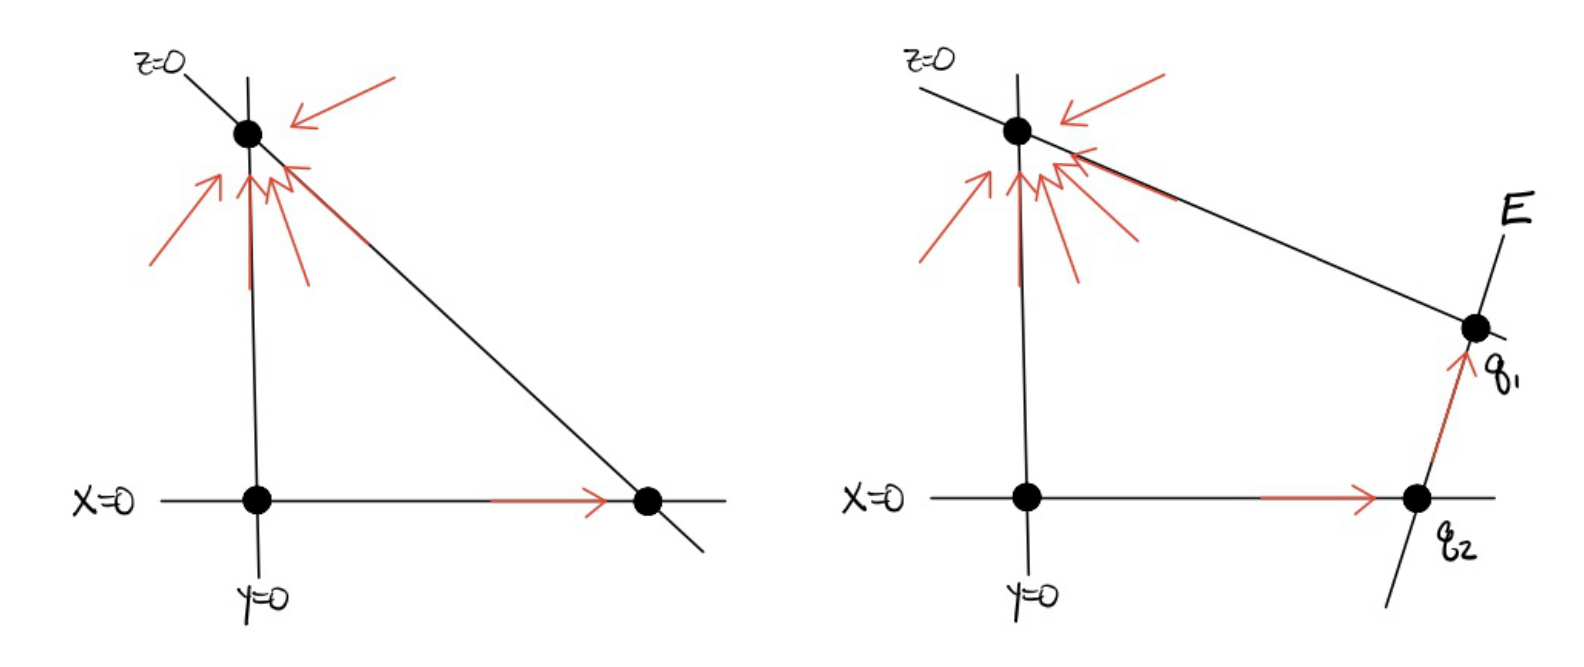
\includegraphics[width=.85\textwidth]{figures/ch07-bb-stratification.png}
\bookfiguretarget{7.8.19}
\caption{$\mathbb P^2$ (左) 与 $\operatorname{Bl}_p\mathbb P^2$ (右) 的 Białynicki--Birula 分层.}\bookfigurehref{7.8.19}\label{src:7.8.19}
\end{figure}

\subsection{Białynicki--Birula 分层在上同调中的应用}\label{src:7.8.4-subsection}
\begin{proposition}\label{src:7.8.20}
设 $X$ 是代数闭域 $\Bbbk$ 上光滑, 不可约, 拟射影的概形, 带有仅有有限个不动点的 $\mathbb G_m$-作用. 则 $\mathrm{CH}_i(X)$ 是由 $i$ 维胞腔的闭包生成的自由 $\mathbb Z$-模. 若 $\Bbbk=\mathbb C$, 则到 Borel--Moore 同调的循环映射 $\mathrm{CH}_i(X)\to H_{2i}^{\mathrm{BM}}(X,\mathbb Z)$ 是同构, 且 $H_{2i+1}^{\mathrm{BM}}(X,\mathbb Z)=0$.
\end{proposition}
\begin{remark}\label{src:7.8.21}
$X$ 紧致时 (如射影时), $H_{2i}^{\mathrm{BM}}(X,\mathbb Z)$ 就是通常的整系数奇异同调.
\end{remark}
\begin{proof}
Białynicki--Birula 分层~\bookref{7.8.14}(4) 说明 $X$ 有胞腔分解, 结论来自 \cite[例 19.1.11]{Ful98}. 另见 \cite[\S3.2]{Bri97}.
\end{proof}
\begin{example}[$\Hilb^n(\mathbb A^2)$ 的 Chow 群]\label{src:7.8.22}
令 $X=\Hilb^n(\mathbb A^2)$ 为 $n$ 个点的 Hilbert 概形, 它光滑不可约 (见 \bookref{2.5.3}). 自然的 $\mathbb G_m^2$-作用诱导 $X$ 上的作用. 在 $\mathbb G_m\to\mathbb G_m^2$, $t\mapsto(t,t)$ 诱导的作用下, 取值映射 $\operatorname{ev}_0:X^+\to X$ 满射, 且 $\mathbb G_m$-不动点对应于支撑在原点, 由单项式理想 $I$ 定义的子概形 $Z=V(I)\subseteq\mathbb A^2$, 因而只有有限个不动点. 可用命题~\bookref{7.8.20} 计算 $\mathrm{CH}^*(X)$.

对单项式理想 $I\subseteq R:=\Bbbk[x,y]$ 及 $i\ge0$, 定义 $a_i:=\min\{j\mid x^iy^j\in I\}$, 令 $r$ 为使 $a_r>0$ 的最大整数. 则 $a_0\ge\cdots\ge a_r$ 是 $n$ 的分拆, $I=(y^{a_0},xy^{a_1},\ldots,x^{r+1})$. 要计算 $\mathbb G_m$ 在单项式理想处切空间 $T_I=\Hom_R(I,R/I)$ 上的正权重空间 $T_{I,>0}$ 的维数. 此切空间由习题~\bookref{2.5.6} 与 $\Hom_R(I,R/I)$ 等同. 先证明作为 $\mathbb G_m^2$-表示有
\begin{align}\label{src:7.8.23}
T_I=\sum_{0\le i\le j\le r}\sum_{s=a_{j+1}}^{a_j-1}\bigl(\chi_1^{i-j-1}\chi_2^{a_i-s-1}+\chi_1^{j-i}\chi_2^{s-a_i}\bigr),
\end{align}
其中 $\chi_i:\mathbb G_m^2\to\mathbb G_m$ 为 $(t_1,t_2)\mapsto t_i^{-1}$ 给出的一维表示. 右侧出现
\begin{align*}
\sum_{0\le i\le j\le r}2(a_j-a_{j+1})=2\sum_{0\le i\le r}a_i=2n=\dim T_I
\end{align*}
个一维表示, 且线性无关. 只需证明每个都出现于 $T_I$. $R$-模映射 $\phi:I\to R/I$ 由 $\phi(x^iy^{a_i})$ 决定, 满足关系
\begin{align*}
\phi(x^{i+1}y^{a_i})=x\phi(x^iy^{a_i}),\qquad\phi(x^iy^{a_{i-1}})=y^{a_{i-1}-a_i}\phi(x^iy^{a_i}).
\end{align*}
对 $0\le i\le j\le r$, $a_{j+1}\le s<a_j$, 定义
\begin{align*}
\phi_{i,j,s}:I\to R/I,\quad x^ly^{a_l}&\longmapsto\begin{cases}x^{l+j-i}y^{a_l+s-a_i},&l\le i,\\0,&\text{其他情形},\end{cases}\\
\psi_{i,j,s}:I\to R/I,\quad x^ly^{a_l}&\longmapsto\begin{cases}x^{l+i-j-1}y^{a_l+s-a_i},&l\ge j+1,\\0,&\text{其他情形}.\end{cases}
\end{align*}
可检验它们是 $R$-模映射, 分别为 $\chi_1^{j-i}\chi_2^{s-a_i}$ 与 $\chi_1^{i-j-1}\chi_2^{a_i-s-1}$ 的特征向量, 故 \bookeqref{7.8.23} 成立.

取 $\lambda=(\lambda_1,\lambda_2):\mathbb G_m\to\mathbb G_m^2$, $\lambda_1\gg\lambda_2$. 按我们的符号约定, \bookeqref{7.8.23} 中特征标 $\chi_1^a\chi_2^b$ 关于 $\lambda$ 的权重为正, 当且仅当 $a<0$, 或 $a=0,b<0$. 因而
\begin{align*}
T_{I,>0}=\sum_{0\le i\le j\le r}\sum_{s=a_{j+1}}^{a_j-1}\chi_1^{i-j-1}\chi_2^{a_i-s-1}+\sum_{j=0}^r\sum_{s=a_{j+1}}^{a_j-1}\chi_1^{j-i}\chi_2^{s-a_i},
\end{align*}
且
\begin{align*}
\dim T_{I,>0}&=\Bigl(\sum_{i=0}^r\sum_{j=i}^r(a_j-a_{j+1})\Bigr)+\Bigl(\sum_{j=0}^r(a_j-a_{j+1})\Bigr)\\
&=\Bigl(\sum_{i=0}^ra_i\Bigr)+a_0=n+a_0.
\end{align*}
因满足 $\dim_{\Bbbk}R/I=n$ 的单项式理想与 $n$ 的分拆 $a_0\ge\cdots\ge a_r$ 双射, 对每个 $d\ge0$, 满足 $\dim T_{I,>0}=d$ 的单项式理想个数等于
\begin{align}\label{src:7.8.24}
P(2n-d,d-n):=\#\{2n-d\text{ 的分拆 }a_1\ge\cdots\ge a_r\mid a_i\le d-n\}.
\end{align}
由命题~\bookref{7.8.20}, 得 $\dim\mathrm{CH}_d(\Hilb^n(\mathbb A^2))_{\mathbb Q}=P(2n-d,d-n)$. 另见 \cite[定理 1.1]{ES87} 与 \cite[\S2.2]{Göt94}.
\end{example}
\begin{exercise}[$\Hilb^n(\mathbb P^2)$ 的 Chow 群]\label{src:7.8.25}
依照上述策略证明 $\Hilb^n(\mathbb P^2)$ 的第 $d$ 个 Betti 数 $b_d$ (等价地, $\dim\mathrm{CH}_d(\Hilb^n(\mathbb P^2))$) 等于
\begin{align*}
b_d=\sum_{n_0+n_1+n_2=n}\sum_{p+r=d-n_1}P(p,n_0-p)P(n_1)P(2n_2-r,r-n_2),
\end{align*}
其中 $P(a)$ 为 $a$ 的分拆数, $P(a,b)$ 由 \bookeqref{7.8.24} 定义.
\end{exercise}
\begin{remark}\label{src:7.8.26}
Göttsche 在 \cite[定理 0.1]{Göt90} 中利用 Weil 猜想 (另见 \cite[定理 2.3.10]{Göt94}), 证明 $\mathbb C$ 或 $\overline{\mathbb F}_q$ 上任意光滑射影曲面 $S$ 的 $S^{[n]}:=\Hilb^n(S)$ 的 Poincaré 多项式 $p(S^{[n]},z)=\sum_i b_i(S^{[n]})z^n$ 满足
\begin{align*}
\sum_{n=0}^{\infty}p(S^{[n]},z)t^n
=\prod_{m=1}^{\infty}\frac{(1+z^{2m-1}t^m)^{b_1(S)}(1+z^{2m+1}t^m)^{b_3(S)}}{(1-z^{2m-2}t^m)^{b_0(S)}(1-z^{2m}t^m)^{b_2(S)}(1-z^{2m+2}t^m)^{b_4(S)}}.
\end{align*}
特别地, $S^{[n]}$ 的 Betti 数只依赖 $S$ 的 Betti 数. 各个 $p(S^{[n]},z)$ 未必有特别好的表达式, 但涉及所有 $n$ 的生成函数有. 另一方面, Nakajima 构造了 Heisenberg 代数在 $H_*(S^{[n]})$ 上的作用, 可用于恢复上述公式及上同调环的更多性质 \cite{Nak97} (另见 \cite{Nak99b}).
\end{remark}
Białynicki--Birula 分层也可用于计算等变 Chow 环 $\mathrm{CH}_G^*(X)$; 见习题~\bookref{8.7.12}.

\section{代数叠的赋值判据: \texorpdfstring{$\Theta$}{Θ}-完备性与 S-完备性}\label{src:7.9}
\begin{epigraph}
你或许会低估定义在数学中的重要性, 但你不应该这样做.
\epigraphauthor{Claire Voisin}
\end{epigraph}
我们讨论 $\Theta$-完备性与 S-完备性的赋值判据 (见定义~\bookref{7.9.10} 和~\bookref{7.9.14}); 它们在下节的良模空间存在性定理~\bookref{7.10.1} 中起核心作用.
\subsection{从 \texorpdfstring{$\Theta=[\mathbb A^1/\mathbb G_m]$}{Θ=[A1/Gm]} 出发的映射}\label{src:7.9.1-subsection}
在 $\Spec\mathbb Z$ 上定义叠 ``Theta'' 为
\[\Theta:=[\mathbb A^1/\mathbb G_m].\]
\footnote{使用符号 $\Theta$ 是因为它的形状类似于 $\mathbb G_m$ 在复平面上的两个轨道的图像.}
在域 $\Bbbk$ 上工作时, 我们也用 $\Theta$ 表示 $\Theta_{\Bbbk}=[\mathbb A^1_{\Bbbk}/\mathbb G_{m,\Bbbk}]$. 从代数叠出发的映射 $\mathcal X\to\Theta$ 由线丛及其截面分类 (例~\bookref{4.9.25}), 而从 $\Theta$ 出发的映射 $\Theta\to\mathcal X$ 往往也有几何意义, 例如 $\mathcal X$ 是商叠, 凝聚层叠或全体曲线的叠时. 这些描述有助于理解第~\bookref{7.9.2-subsection} 节引入的 $\Theta$-完备性与 S-完备性的赋值判据.

\textbf{商叠.} 给定商叠 $[X/G]$, 单参数子群 $\lambda:\mathbb G_m\to G$ 和一点 $x\in X(\Bbbk)$, 若 $\lim_{t\to0}\lambda(t)\cdot x\in X$ 存在, 则 $\mathbb G_m$-等变延拓 $\mathbb A^1\to X$ 诱导代数叠的态射 $[\mathbb A^1/\mathbb G_m]\to[X/G]$. 下述命题断言逆命题也成立: 每个这样的映射均由单参数子群 $\lambda$ 和一点 $x\in X(\Bbbk)$ 诱导. 回忆 $C_\lambda$ 表示 $\lambda$ 的中心化子, $P_\lambda$ 是满足 $\lim_{t\to0}\lambda(t)g\lambda(t)^{-1}$ 存在的元素 $g\in G$ 组成的子群; 见第~\bookref{B.1.4-subsection} 节.
\begin{proposition}\label{src:7.9.1}
设代数闭域 $\Bbbk$ 上的光滑仿射代数群 $G$ 作用在 $\Bbbk$ 上有限型分离代数空间 $X$ 上. 则有群胚的等价
\[\operatorname{Mor}_{\Bbbk}(\Theta,[X/G])\xrightarrow{\sim}
\{(x\in X(\Bbbk),\lambda:\mathbb G_m\to G)\mid\lim_{t\to0}\lambda(t)\cdot x\in X(\Bbbk)\text{ 存在}\}.\]
态射 $(x,\lambda)\to(x',\lambda')$ 是二元组 $(g,h)$ 的同构类, 其中 $g\in P_\lambda(\Bbbk)$, $h\in G(\Bbbk)$, $x'=hgx$, $\lambda'=h\lambda h^{-1}$, 且对 $c\in C_\lambda$ 有 $(g,h)\sim(c^{-1}g,hc)$. 在此对应下, $\Theta\to[X/G]$ 将 $1$ 送到 $x$, 将 $0$ 送到 $\lim_{t\to0}\lambda(t)\cdot x$.
\end{proposition}
\begin{remark}\label{src:7.9.2}
注意 $(x,\lambda)$ 的自同构群为 $P_\lambda\cap G_x$.
\end{remark}
\begin{proof}
给定 $(x,\lambda)$, 由 $t\mapsto\lambda(t)\cdot x$ 定义的 $\mathbb G_m$-等变映射 $m_{x,\lambda}:\mathbb G_m\to X$ 延拓为交换图
\[\begin{tikzcd}[ampersand replacement=\&]\mathbb G_m\arrow[r,"{m_{x,\lambda}}"]\arrow[d,hook]\&X\\\mathbb A^1\arrow[ur,"{\widetilde m_{x,\lambda}}"']\&\end{tikzcd}\]
此延拓 $\mathbb G_m$-等变, 因而诱导商叠的态射 $f_{x,\lambda}:\Theta\to[X/G]$. 先证明这定义了函子
\begin{align}\label{src:7.9.3}
\{(x,\lambda)\mid\lim_{t\to0}\lambda(t)\cdot x\text{ 存在}\}&\longrightarrow\operatorname{Mor}_{\Bbbk}(\Theta,[X/G]),& (x,\lambda)&\longmapsto f_{x,\lambda}.
\end{align}
给定态射 $(g,h):(x,\lambda)\to(x',\lambda')$, 需要定义 $2$-态射 $f_{x,\lambda}\xrightarrow{\sim}f_{x',\lambda'}$. 因 $h$ 确定典范同构 $f_{x',\lambda'}\xrightarrow{\sim}f_{h^{-1}x',\lambda}$, 只需定义 $f_{x,\lambda}\xrightarrow{\sim}f_{h^{-1}x',\lambda}$. 因 $g\in P_\lambda(\Bbbk)$, 映射 $t\mapsto\lambda(t)g\lambda(t)^{-1}$ 延拓为 $\widetilde g:\mathbb A^1\to G$, 且 $\widetilde m_{h^{-1}x',\lambda}=\widetilde g\cdot\widetilde m_{x,\lambda}$, 因为 $h^{-1}x'=gx$. 元素 $\widetilde g$ 定义所需同构. 对 $c\in C_\lambda$, 二元组 $(g,h)$ 与 $(c^{-1}g,hc)$ 定义相同同构: 若 $c\in G_x$, 则 $(c^{-1},c)$ 定义 $f_{x,\lambda}$ 的恒等自同构. 反之, 每个同构 $f_{x,\lambda}\xrightarrow{\sim}f_{x',\lambda}$ 都由满足 $\widetilde m_{x',\lambda}=\widetilde g\cdot\widetilde m_{x,\lambda}$ 的元素 $\widetilde g\in G(\mathbb A^1)$ 诱导. 因而~\bookeqref{7.9.3} 是全忠实函子.

为证明本质满性, 设 $f:\Theta\to[X/G]$ 是态射. 在纤维图
\[\begin{tikzcd}[ampersand replacement=\&]\mathcal P\arrow[r]\arrow[d]\&X\arrow[d]\\\Theta\arrow[r,"{f}"]\&{[X/G]}\end{tikzcd}\]
中, $\mathcal P\to\Theta$ 是主 $G$-丛. 沿唯一闭点 $0\in\Theta$ 的限制 $\mathcal P|_{B\mathbb G_m}$ 对应于 $\Spec\Bbbk$ 上的 $\mathbb G_m$-等变主 $G$-丛 $P$. 选择同构 $P\cong G$ 后, $\mathcal P$ 对应于单参数子群 $\lambda:\mathbb G_m\to G$. 它在 $\mathbb A^1\times G$ 上诱导作用 $t\cdot(x,g)=(tx,g\lambda(t)^{-1})$, 从而给出主 $G$-丛
\[\mathcal P_\lambda:=[(\mathbb A^1\times G)/\mathbb G_m]\to\Theta.\]
断言存在主 $G$-丛的同构 $\alpha:\mathcal P\to\mathcal P_\lambda$. 按构造有同构 $\alpha_0:\mathcal P|_{B\mathbb G_m}\to\mathcal P_\lambda|_{B\mathbb G_m}$. 因为 $\underline{\operatorname{Isom}}_\Theta(\mathcal P,\mathcal P_\lambda)\to\Theta$ 光滑 (它是主 $G$-丛且 $G$ 光滑), 变形理论 (命题~\bookref{7.7.12}) 给出 $B\mathbb G_m\hookrightarrow\Theta$ 的幂零加厚 $\mathcal X_n$ 上相容的同构 $\alpha_n:\mathcal P|_{\mathcal X_n}\to\mathcal P_\lambda|_{\mathcal X_n}$. 凝聚 Tannaka 对偶性~\bookref{7.6.9} 与 $\Theta$ 沿 $B\mathbb G_m$ 的凝聚完备性 (定理~\bookref{7.6.13}) 将它们延拓为同构 $\alpha:\mathcal P\to\mathcal P_\lambda$. 将复合
\[\mathbb A^1\times G\to\mathcal P_\lambda\xrightarrow{\alpha^{-1}}\mathcal P\to X\]
限制到 $G$ 的单位元, 得到 $\mathbb G_m$-等变态射 $\mathbb A^1\to X$, 从而诱导映射 $f:\Theta\to[X/G]$. 令 $x$ 是 $1$ 的像, 可核实 $f_{x,\lambda}$ 与 $f$ 是 $2$-同构的.
\end{proof}
\begin{exercise}[细节]\label{src:7.9.4}
令 $R$ 为完备Noether局部 $\Bbbk$-代数, 将该命题推广为 $\operatorname{Mor}_{\Bbbk}(\Theta_R,[X/G])$ 与二元组 $(x\in X(R),\lambda:\mathbb G_m\to G)$ 之间的等价.
\end{exercise}
\begin{remark}\label{src:7.9.5}
命题~\bookref{7.9.1} 还可推广为从 $[\mathbb A^1/\mathbb G_m]$ 到 $[X/G]$ 的态射叠的描述. 即有分解
\[\underline{\operatorname{Mor}}([\mathbb A^1/\mathbb G_m],[X/G])\cong\coprod_\lambda[X_\lambda^+/P_\lambda],\]
其中 $\lambda$ 遍历单参数子群的共轭类. 此叠的代数性已在注~\bookref{7.8.13} 中讨论; 另见 \cite[定理~1.37]{HL14}.
\end{remark}
\textbf{凝聚层叠.} 对域 $\Bbbk$ 上的概形 $X$, 用 $\Coh(X)$ 表示 $X$ 上凝聚层的叠. 若 $X$ 射影 (分别地, 固有), 则由习题~\bookref{4.1.25} (分别地, 定理~\bookref{C.7.7}), $\Coh(X)$ 是代数叠.
\begin{proposition}\label{src:7.9.6}
设 $X$ 是域 $\Bbbk$ 上的概形. 对Noether $\Bbbk$-代数 $R$, $\operatorname{Mor}_{\Bbbk}(\Theta_R,\Coh(X))$ 等价于二元组 $(E,E_\bullet)$ 的群胚, 其中 $E$ 是 $X_R$ 上在 $R$ 上平坦的凝聚层,
\[E_\bullet:0\subseteq\cdots\subseteq E_{i-1}\subseteq E_i\subseteq E_{i+1}\subseteq\cdots\subseteq E\]
是 $\mathbb Z$-分次滤过, 满足 $i\ll0$ 时 $E_i=0$, $i\gg0$ 时 $E_i=E$, 且每个因子 $E_i/E_{i-1}$ 在 $R$ 上平坦. 态射 $(E,E_\bullet)\to(E',E'_\bullet)$ 是与滤过相容的凝聚层同构 $E\to E'$. 此对应将 $1$ 送到 $E$, 将 $0$ 送到相伴分次 $\operatorname{gr}E_\bullet:=\bigoplus_iE_i/E_{i-1}$. 映射经由 $\cBun(X)\subseteq\Coh(X)$ 分解当且仅当 $E$ 与每个因子 $E_i/E_{i-1}$ 都是向量丛.
\end{proposition}
\begin{proof}
读者可先阅读特殊但重要的情形 $R=\Bbbk$. 态射 $\Theta_R\to\Coh(X)$ 对应于 $X\times\Theta_R$ 上在 $\Theta_R$ 上平坦的凝聚层 $F$, 也对应于 $X\times\mathbb A_R^1$ 上在 $\mathbb A_R^1$ 上平坦, 带相容 $\mathbb G_m$-作用的凝聚层. 因为 $f:X\times\Theta_R\to X\times B\mathbb G_{m,R}$ 仿射, 可由拟凝聚层 $f_*F$ 及其 $f_*\mathcal O_{X\times\Theta_R}$-模结构恢复 $F$. $X\times B\mathbb G_{m,R}$ 上的拟凝聚层是 $X_R$ 上的 $\mathbb Z$-分次拟凝聚层 (习题~\bookref{7.1.10}), 因而 $F$ 对应于在 $R[x]$ 上平坦的 $\mathbb Z$-分次 $\mathcal O_{X_R}[x]$-模. 写成 $F=\bigoplus_{i\in\mathbb Z}E_i$, 每个 $E_i$ 是 $X_R$ 上的凝聚层, 则乘以 $x$ 诱导 $x:E_i\to E_{i+1}$. 由于 $F$ 在 $R[x]$ 上平坦, 从而无挠, 这些映射单射. $F$ 作为分次 $R[x]$-模有限生成, 所以存在有限多个次数有界的齐次生成元. 因而 $i\gg0$ 时 $E_i=E$. 另一方面, 考虑 $\mathcal O_{X_R}[x]$-子模 $E_{\geq d}:=\bigoplus_{i>d}E_i\subseteq F$. 因 $F$ Noether, 升链 $\cdots\subseteq E_{\geq d}\subseteq E_{\geq d-1}\subseteq\cdots\subseteq F$ 必终止, 因而 $i\ll0$ 时 $E_i=0$. $F$ 在 $R[x]$ 上平坦, 故商 $F/xF=\bigoplus_iE_i/E_{i-1}$ 在 $R$ 上平坦, 每个因子亦然.

反之, 给定满足条件的 $E$ 与 $E_\bullet$, 考虑分次 $\mathcal O_{X_R}[x]$-模 $F:=\bigoplus_iE_i$, 通常称为 Rees 构造. 归纳证明 $E_{\geq d}:=\bigoplus_{i\geq d}E_i$ 在 $R[x]$ 上平坦且有限生成; 因 $i\ll0$ 时 $E_i=0$, 这便证明了 $F$ 的相应性质. 当 $d\gg0$, $E_{\geq d}$ 同构于分次 $R[x]$-模 $(E\otimes_RR[x])\langle d\rangle$, 其中 $\langle d\rangle$ 表示分次移位, 所以平坦且有限生成. 对每个 $d$ 有正合列
\[0\to(E_d\otimes_RR[x])\langle d\rangle\to E_{\geq d}\to((E_{d+1}/E_d)\otimes_RR[x])\langle d+1\rangle\to0.\]
$E$ 与商 $E_{d+1}/E_d$ 的平坦性蕴含每个 $E_d$ 的平坦性. 因而左右两项在 $R[x]$ 上平坦且有限生成, 中间项亦然.
\end{proof}
\textbf{全体曲线的叠.}
\begin{proposition}\label{src:7.9.7}
设 $\mathcal M_g^{\mathrm{all}}$ 是代数闭域 $\Bbbk$ 上全体固有曲线的代数叠 (定理~\bookref{6.4.6}). 对每个 $\Bbbk$-代数 $R$, 群胚 $\operatorname{Mor}_{\Bbbk}(\Theta_R,\mathcal M_g^{\mathrm{all}})$ 的对象是 $\mathbb G_m$-等变固有曲线族 $\mathcal C\to\mathbb A_R^1$, 其中 $\mathbb G_m$ 在 $\mathbb A_R^1$ 上作通常的缩放作用; 态射是 $\mathbb G_m$-等变态射.
\end{proposition}
\begin{proof}
对 $\mathbb A_R^1\to\Theta_R$ 应用光滑下降即可.
\end{proof}
\begin{remark}\label{src:7.9.8}
其他簇的模叠也有类似描述. 文献中通常将这些 $\mathbb G_m$-等变族称为\newterm{检验构形}{test configuration}.
\end{remark}
\subsection{赋值判据: \texorpdfstring{$\Theta$}{Θ}-完备性与 S-完备性}\label{src:7.9.2-subsection}
仍记 $\Theta:=[\mathbb A^1/\mathbb G_m]$, 定义在 $\Spec\mathbb Z$ 上. 设 $R$ 是分式域为 $K$, 剩余域为 $\kappa$ 的 DVR. 定义 $\Theta_R:=\Theta\times\Spec R$, 令 $0\in\Theta_R$ 为唯一闭点. $\Theta_R$ 是权重为 $0,1$ 的商叠 $[\mathbb A^2/\mathbb G_m]$ 的局部模型: 它是良模空间 $[\mathbb A^2/\mathbb G_m]\to\Spec\Bbbk[x]$ 沿 $x\mapsto\pi$ 所给映射 $\Spec R\to\Spec\Bbbk[x]$ 的基变换, 其中 $\pi$ 是 $R$ 的一致化元. 以下笛卡尔图示意地描述 $\Theta_R$ ($x$ 是 $\mathbb A^1$ 的坐标):
\begin{align}\label{src:7.9.9}
\begin{tikzcd}[ampersand replacement=\&,column sep=small,row sep=large]
\&\Spec R\arrow[dr,hook,"{x\ne0}"]\&\&B\mathbb G_{m,R}\arrow[dl,hook',"{x=0}"']\&\\
\Spec K\arrow[ur,hook]\arrow[dr,hook]\& \&\Theta_R\&\&B\mathbb G_{m,\kappa}\arrow[ul,hook']\arrow[dl,hook]\\
\&\Theta_K\arrow[ur,hook,"{\pi\ne0}"']\&\&\Theta_\kappa\arrow[ul,hook',"{\pi=0}"]\&
\end{tikzcd}
\end{align}
左侧箭头为开浸入, 右侧箭头为闭浸入. 特别地, 到代数叠的态射 $\Theta_R\setminus0=\Spec R\cup_{\Spec K}\Theta_K\to\mathcal X$ 等价于态射 $\Spec R\to\mathcal X$ 与 $\Theta_K\to\mathcal X$, 以及它们在 $\Spec K$ 上的限制之间的同构.
\begin{definition}\label{src:7.9.10}
若对每个 DVR $R$, 每个实线箭头组成的交换图
\begin{align}\label{src:7.9.11}
\begin{tikzcd}[ampersand replacement=\&]\Theta_R\setminus0\arrow[r]\arrow[d]\&\mathcal X\\\Theta_R\arrow[ur,dashed]\&\end{tikzcd}
\end{align}
都能唯一补全, 则称Noether代数叠 $\mathcal X$ 为\newterm{$\Theta$-完备}{$\Theta$-complete} 的.\footnote{这一概念引入于 \cite{HL14}, 当时称为 ``$\Theta$-约化'' ($\Theta$-reductive).}
\end{definition}
\begin{remark}\label{src:7.9.12}
等价地, 用分类态射 $\Theta\to\mathcal X$ 的叠 $\underline{\operatorname{Mor}}(\Theta,\mathcal X)$, 在 $1$ 处的取值给出态射
\[\mathrm{ev}_1:\underline{\operatorname{Mor}}(\Theta,\mathcal X)\to\mathcal X,\qquad f\mapsto f(1).\]
$\mathcal X$ 是 $\Theta$-完备的当且仅当 $\mathrm{ev}_1$ 满足固有性的赋值判据. 若 $\mathcal X$ 在代数闭域 $\Bbbk$ 上有限型, 则 $\underline{\operatorname{Mor}}(\Theta,\mathcal X)$ 是 $\Bbbk$ 上局部有限型代数叠; 商叠情形的显式描述见注~\bookref{7.9.5}. 但此叠很少拟紧, 例如 $\mathcal X=B\mathbb G_m$ 时, 因而 $\mathrm{ev}_1$ 很少固有.
\end{remark}
对分式域为 $K$, 剩余域为 $\kappa$, 一致化元为 $\pi$ 的 DVR $R$, 定义
\begin{align}\label{src:7.9.13}
\phi_R:=[\Spec(R[s,t]/(st-\pi))/\mathbb G_m],
\end{align}
其中 $s,t$ 的 $\mathbb G_m$-权重分别为 $1,-1$.\footnote{使用符号 $\phi$ 是因为它看起来像增加了一个原点的非分离仿射直线. 此叠引入于 \cite[第~2.B 节]{Hei17}, 记作 $\overline{\mathrm{ST}}_R$, 因为它是分离性的 ``标准检验'' 概形 $\mathrm{ST}_R=\overline{\mathrm{ST}}_R\setminus0=\Spec R\cup_{\Spec K}\Spec R$ 的紧化.}
它是权重为 $1,-1$ 的商叠 $[\mathbb A^2/\mathbb G_m]$ 的局部模型, 等同于良模空间 $[\mathbb A^2/\mathbb G_m]\to\Spec\Bbbk[xy]$ 沿 $xy\mapsto\pi$ 所给映射 $\Spec R\to\Spec\Bbbk[xy]$ 的基变换. $\phi_R$ 中 $s\ne0$ 的轨迹同构于 $[\Spec(R[s,t]_s/(t-\pi/s))/\mathbb G_m]\cong[\Spec(R[s]_s)/\mathbb G_m]\cong\Spec R$, $t\ne0$ 的轨迹有类似描述. 因而有类似于~\bookeqref{7.9.9} 的笛卡尔图
\[\begin{tikzcd}[ampersand replacement=\&,column sep=small,row sep=large]
\&\Spec R\arrow[dr,hook,"{s\ne0}"]\&\&\Theta_\kappa\arrow[dl,hook',"{s=0}"']\&\\
\Spec K\arrow[ur,hook]\arrow[dr,hook]\&\&\phi_R\&\&B\mathbb G_{m,\kappa}\arrow[ul,hook']\arrow[dl,hook]\\
\&\Spec R\arrow[ur,hook,"{t\ne0}"']\&\&\Theta_\kappa\arrow[ul,hook',"{t=0}"]\&
\end{tikzcd}\]
左侧箭头是开浸入, 右侧箭头是闭浸入. 特别地, 到代数叠的态射 $\phi_R\setminus0=\Spec R\cup_{\Spec K}\Spec R\to\mathcal X$ 等价于两个态射 $\xi,\xi':\Spec R\to\mathcal X$ 及在 $\Spec K$ 上的同构 $\xi_K\simeq\xi'_K$.
\begin{definition}\label{src:7.9.14}
若对每个 DVR $R$, 每个实线箭头组成的交换图
\begin{align}\label{src:7.9.15}
\begin{tikzcd}[ampersand replacement=\&]\phi_R\setminus0\arrow[r]\arrow[d]\&\mathcal X\\\phi_R\arrow[ur,dashed]\&\end{tikzcd}
\end{align}
都能唯一补全, 则称Noether代数叠 $\mathcal X$ 为\newterm{S-完备}{S-complete} 的.\footnote{``S'' 代表 ``Seshadri'': S-完备性是一种几何性质, 令人联想到层的 S-等价关系如何蕴含模空间的分离性.}
\end{definition}
$\Theta$-完备性与 S-完备性的定义自然延伸到态射 $f:\mathcal X\to\mathcal Y$, 但我们不会使用这一推广.
\begin{exercise}\label{src:7.9.16}
设 $X$ 是 $\Bbbk$-概形, $R$ 是 $\Bbbk$ 上的 DVR.
\begin{enumerate}[(1)]
\item 证明 $X\times\phi_R$ 上的拟凝聚层 $\mathcal F$ 对应于 $X_R$ 上的 $\mathbb Z$-分次拟凝聚层 $\bigoplus_{n\in\mathbb Z}\mathcal F_n$ 及映射图
\[\begin{tikzcd}[ampersand replacement=\&]\cdots\arrow[r,bend left,"{s}"]\&\mathcal F_{n-1}\arrow[l,bend left,"{t}"]\arrow[r,bend left,"{s}"]\&\mathcal F_n\arrow[l,bend left,"{t}"]\arrow[r,bend left,"{s}"]\&\mathcal F_{n+1}\arrow[l,bend left,"{t}"]\arrow[r,bend left,"{s}"]\&\cdots\arrow[l,bend left,"{t}"]\end{tikzcd}\]
满足 $st=ts=\pi$.
\item 证明若每个 $\mathcal F_n$ 凝聚, $n\gg0$ 时 $s:\mathcal F_{n-1}\to\mathcal F_n$ 是同构, $n\ll0$ 时 $t:\mathcal F_n\to\mathcal F_{n-1}$ 是同构, 则 $\mathcal F$ 凝聚. 证明若 $s,t$ 单射, 则逆命题成立.
\item 证明 $\mathcal F$ 在 $\phi_R$ 上平坦当且仅当 $s,t$ 单射, 且诱导映射 $t:\mathcal F_{n+1}/s\mathcal F_n\to\mathcal F_n/s\mathcal F_{n-1}$ 单射.
\item 假设 $\mathcal F$ 凝聚且在 $\phi_R$ 上平坦, 如下刻画其限制:
\begin{enumerate}[(i)]
\item $X_R$ 上的 $\mathcal F|_{\{s\ne0\}}\cong\operatorname{colim}(\cdots\xrightarrow{s}\mathcal F_n\xrightarrow{s}\mathcal F_{n+1}\xrightarrow{s}\cdots)$;
\item $X_R$ 上的 $\mathcal F|_{\{t\ne0\}}\cong\operatorname{colim}(\cdots\xrightarrow{t}\mathcal F_{n+1}\xrightarrow{t}\mathcal F_n\xrightarrow{t}\cdots)$;
\item $\Theta_\kappa$ 上的 $\mathcal F|_{\{s=0\}}$ 在命题~\bookref{7.9.6} 下对应于 $\mathbb Z$-滤过 $\cdots\xrightarrow{t}\mathcal F_{n+1}/s\mathcal F_{n+2}\xrightarrow{t}\mathcal F_n/s\mathcal F_{n-1}\xrightarrow{t}\cdots$;
\item $\Theta_\kappa$ 上的 $\mathcal F|_{\{t=0\}}$ 对应于 $\mathbb Z$-滤过 $\cdots\xrightarrow{s}\mathcal F_n/t\mathcal F_{n+1}\xrightarrow{s}\mathcal F_{n+1}/t\mathcal F_{n+2}\xrightarrow{s}\cdots$.
\end{enumerate}
\end{enumerate}
\end{exercise}
\subsection{\texorpdfstring{$\Theta$}{Θ}-完备性与 S-完备性的性质}\label{src:7.9.3-subsection}
\begin{lemma}\label{src:7.9.17}
具有仿射对角态射的Noether代数叠是 $\Theta$-完备的 (分别地, S-完备的), 当且仅当每个图~\bookeqref{7.9.11} (分别地, 图~\bookeqref{7.9.15}) 都在 DVR 扩张 $R\subseteq R'$ 后存在提升. 特别地, 两种完备性均可在剩余域代数闭的完备 DVR 上检验.
\end{lemma}
\begin{proof}
先观察: 若 $\mathcal X\to\mathcal Y$ 具有仿射对角态射, $j:\mathcal U\to\mathcal T$ 是 $\mathcal Y$ 上代数叠的开浸入, 且 $j_*\mathcal O_{\mathcal U}=\mathcal O_{\mathcal T}$, 则 $\mathcal Y$-态射 $\mathcal U\to\mathcal X$ 的两个延拓 $f_1,f_2:\mathcal T\to\mathcal X$ 典范地 $2$-同构. 因为 $\underline{\operatorname{Isom}}_{\mathcal T}(f_1,f_2)\to\mathcal T$ 仿射, $2$-同构 $f_1|_{\mathcal U}\xrightarrow{\sim}f_2|_{\mathcal U}$ 诱导的截面唯一延拓为 $\mathcal T$ 上的截面.

考虑图~\bookeqref{7.9.11}, DVR 扩张 $R\subseteq R'$ 及提升 $\Theta_{R'}\to\mathcal X$. 开浸入 $j:\Theta_R\setminus0\to\Theta_R$ 满足 $j_*\mathcal O_{\Theta_R\setminus0}=\mathcal O_{\Theta_R}$; 由平坦基变换~\bookref{7.1.14}, 沿 $\Theta_{R'}\to\Theta_R$, $\Theta_{R'}\times_{\Theta_R}\Theta_{R'}\to\Theta_R$ 及三重纤维积到 $\Theta_R$ 的态射作基变换后, 同一性质仍成立. 上述观察给出两个延拓 $\Theta_{R'}\times_{\Theta_R}\Theta_{R'}\rightrightarrows\Theta_{R'}\to\mathcal X$ 之间的典范 $2$-同构, 必满足余循环条件. 由 fpqc 下降, 提升下降为 $\Theta_R\to\mathcal X$. S-完备性的论证相同.
\end{proof}
\begin{remark}\label{src:7.9.18}
当 $\mathcal X$ 在 $\Bbbk$ 上有限型时, 这些判据也可在 $\Bbbk$ 上本质有限型的 DVR 上检验; 见 \cite[第~4 节]{AHLH23}. 我们不使用这一事实.
\end{remark}
\begin{lemma}\label{src:7.9.19}
设 $f:\mathcal X\to\mathcal Y$ 是Noether代数叠的仿射态射. 若 $\mathcal Y$ 是 $\Theta$-完备的 (分别地, S-完备的), 则 $\mathcal X$ 亦然.
\end{lemma}
\begin{proof}
$\Theta_R$ 正则且 $0\in\Theta_R$ 的余维为 $2$, 因而结构层沿 $\Theta_R\setminus0\to\Theta_R$ 的推前仍是结构层. 所以有典范等价
\begin{align*}
\operatorname{Mor}_{\mathcal Y}(\Theta_R\setminus0,\mathcal X)
&\cong\operatorname{Mor}_{\mathcal O_{\mathcal Y}\text{-alg}}(f_*\mathcal O_{\mathcal X},(\Theta_R\setminus0\to\mathcal Y)_*\mathcal O_{\Theta_R\setminus0})\\
&\cong\operatorname{Mor}_{\mathcal O_{\mathcal Y}\text{-alg}}(f_*\mathcal O_{\mathcal X},(\Theta_R\to\mathcal Y)_*\mathcal O_{\Theta_R})\\
&\cong\operatorname{Mor}_{\mathcal Y}(\Theta_R,\mathcal X).
\end{align*}
S-完备性的情形完全相同.
\end{proof}
\begin{proposition}\label{src:7.9.20}
若 $G$ 是代数闭域 $\Bbbk$ 上的约化群, 则每个商叠 $[\Spec A/G]$ 都是 $\Theta$-完备且 S-完备的.
\end{proposition}
\begin{proof}
先证明 $B\mathrm{GL}_n$ 是 $\Theta$-完备的. 态射 $\Theta_R\setminus0\to\mathcal X$ 对应于 $\Theta_R\setminus0$ 上的向量丛 $E$. 叠 $\Theta_R$ 正则, $0$ 的余维为 $2$. 若 $\widetilde E$ 是延拓 $E$ 的凝聚层, 则双对偶 $\widetilde E^{\vee\vee}$ 是延拓 $E$ 的向量丛. (事实上 $E$ 沿 $\Theta_R\setminus0\hookrightarrow\Theta_R$ 的推前就是向量丛.) 这给出所需延拓 $\Theta_R\to\mathcal X$. 因 $G$ 仿射, 可选择忠实表示 $G\subseteq\mathrm{GL}_n$. 因 $G$ 约化, Matsushima 定理~\bookref{B.1.48} 蕴含 $\mathrm{GL}_n/G$ 仿射. 由笛卡尔图
\[\begin{tikzcd}[ampersand replacement=\&]\mathrm{GL}_n/G\arrow[r]\arrow[d]\&BG\arrow[d]\\\Spec\Bbbk\arrow[r]\&B\mathrm{GL}_n\end{tikzcd}\]
及光滑下降可知 $BG\to B\mathrm{GL}_n$ 仿射. 引理~\bookref{7.9.19} 蕴含 $BG$ 和 $[\Spec A/G]$ 是 $\Theta$-完备的. 命题~\bookref{7.10.30} 将证明 $BG$ 是 S-完备的, 由引理~\bookref{7.9.19}, $[\Spec A/G]$ 亦然.
\end{proof}
对环 $R$, 映射 $\Theta_R\to\Spec R$ 是良模空间, 所以由良模空间的泛性质 (定理~\bookref{7.5.11}(4)), 每个到代数空间的映射 $\Theta_A\to X$ 都经由 $\Spec R$ 分解. 当 $X$ 是 Deligne--Mumford 叠时也有类似结论.
\begin{lemma}\label{src:7.9.21}
设Noether代数叠 $\mathcal X$ 具有仿射拟有限对角态射. 若 $R$ 是完备 DVR, 则每个映射 $\Theta_R\to\mathcal X$ (分别地, $\phi_R\to\mathcal X$) 都经由 $\Theta_R\to\Spec R$ (分别地, $\phi_R\to\Spec R$) 分解.
\end{lemma}
\begin{proof}
化归到 $\mathcal X$ 仿射的情形, 此时由 $\Gamma(\Theta_R,\mathcal O_{\Theta_R})=\Gamma(\phi_R,\mathcal O_{\phi_R})=R$ 即得结论. 令 $\kappa=R/\mathfrak m$, 令 $x\in\mathcal X(\kappa)$ 为 $0\in\Theta_R$ 的像. $\mathbb G_m$ 无非平凡有限商, 所以诱导的稳定子映射 $\mathbb G_m\to G_x$ 平凡. 由命题~\bookref{5.3.4}, 可取来自仿射概形的光滑展示 $U\to\mathcal X$ 及 $x$ 的提升 $u\in U(\kappa)$. 映射 $B\mathbb G_{m,\kappa}\to\mathcal X$ 经由 $u:\Spec\kappa\to U$ 分解, 因而提升为 $B\mathbb G_{m,\kappa}\to\Spec\kappa\xrightarrow{u}U$. 令 $\mathcal T_n$ 为 $B\mathbb G_{m,\kappa}\to\Theta_R$ 的第 $n$ 个幂零加厚, 由变形理论 (命题~\bookref{7.7.12}) 可找到 $\mathcal T_n\hookrightarrow\Theta_R\to\mathcal X$ 的相容提升 $\mathcal T_n\to U$. 凝聚 Tannaka 对偶性~\bookref{7.6.9} 给出延拓 $\Theta_R\to U$. 因其经由 $\Spec R$ 分解, $\Theta_R\to\mathcal X$ 也如此.
\end{proof}
\begin{proposition}\label{src:7.9.22}
每个具有仿射拟有限对角态射的Noether代数叠 $\mathcal X$ (例如具有仿射对角态射的 Deligne--Mumford 叠) 都是 $\Theta$-完备的. 此外, $\mathcal X$ 是 S-完备的当且仅当它分离.
\end{proposition}
\begin{proof}
由引理~\bookref{7.9.17}, 可在完备 DVR $R$ 上检验两种完备性. 引理~\bookref{7.9.21} 蕴含 $\Theta$-完备性, 且蕴含 S-完备性等价于每个图
\[\begin{tikzcd}[ampersand replacement=\&]\Spec K\arrow[r]\arrow[d]\&\mathcal X\arrow[d,"{\Delta}"]\\\Spec R\arrow[r]\arrow[ur,dashed]\&\mathcal X\times\mathcal X\end{tikzcd}\]
都有提升, 这正是通常的分离性赋值判据.
\end{proof}
存在分离良模空间的必要条件是 $\Theta$-完备且 S-完备.
\begin{proposition}\label{src:7.9.23}
设 $\mathcal X$ 是代数闭域 $\Bbbk$ 上有限型, 具有仿射对角态射的代数叠. 若 $\pi:\mathcal X\to X$ 是良模空间, 则 $\mathcal X$ 是 $\Theta$-完备的. 此外, $\mathcal X$ 是 S-完备的当且仅当 $X$ 分离.
\end{proposition}
\begin{proof}
因 $X$ 是 $\Theta$-完备的, 只需证明每个实线交换图
\[\begin{tikzcd}[ampersand replacement=\&]\Theta_R\setminus0\arrow[r]\arrow[d]\&\mathcal X\arrow[d,"{\pi}"]\\\Theta_R\arrow[r]\arrow[ur,dashed]\&X\end{tikzcd}\]
存在提升. 由良模空间的局部结构~\bookref{7.7.3}, 存在包含 $\Spec R$ 的像的平展态射 $\Spec B\to X$, 满足 $\mathcal X\times_X\Spec B\cong[\Spec A/G]$, 其中 $G$ 线性约化且 $B=A^G$. $\Spec R\to X$ 在 DVR 扩张后提升到 $\Spec B$, 而完备性可在扩张后检验 (引理~\bookref{7.9.17}), 因而化归到 $[\Spec A/G]$, 即命题~\bookref{7.9.20}.

若 $X$ 分离, 则由分离性赋值判据, $\phi_R\setminus0=\Spec R\cup_{\Spec K}\Spec R\to X$ 经由 $\Spec R$ 分解, 因而 $X$ 是 S-完备的. 同样的论证说明 $\mathcal X$ 是 S-完备的. 反之, 设 $f,g:\Spec R\to X$ 满足 $f|_K=g|_K$. 适当扩张 $R$ 后, 可选择 $f|_K=g|_K$ 的提升 $\Spec K\to\mathcal X$. 因 $\mathcal X\to X$ 普遍闭 (定理~\bookref{7.5.11}(1)), 由普遍闭性的赋值判据~\bookref{4.8.7}, 进一步扩张后可取 $f,g$ 的提升 $\widetilde f,\widetilde g:\Spec R\to X$, 且 $\widetilde f|_K\cong\widetilde g|_K$. S-完备性将两者延拓为 $\phi_R\to\mathcal X$. $\phi_R\to\Spec R$ 是良模空间, 对到代数空间的映射具有泛性质, 所以 $\phi_R\to\mathcal X$ 下降为唯一的 $\Spec R\to X$, 它必同时等于 $f,g$. 分离性赋值判据即蕴含 $X$ 分离.
\end{proof}
\subsection{\texorpdfstring{$\Theta$}{Θ}-完备性与 S-完备性的例子}\label{src:7.9.4-subsection}
讨论商叠, 凝聚层叠以及全体曲线的叠的两种完备性.

\textbf{商叠.} 由命题~\bookref{7.9.1}, 映射 $\Theta\to[U/G]$ 由一点 $u\in U$ 及使 $\lim_{t\to0}\lambda(t)\cdot u$ 存在的单参数子群 $\lambda:\mathbb G_m\to G$ 分类. 据此给出商叠的 $\Theta$-完备性的几何刻画. 对 $\lambda$ 诱导的 $\mathbb G_m$-作用, 吸引子轨迹 $U_\lambda^+$ 是表示函子 $\operatorname{Mor}_{\Bbbk}^{\mathbb G_m}(\mathbb A^1,U)$ 的代数空间 (定理~\bookref{7.8.9}); 取值映射 $\mathrm{ev}_1:U_\lambda^+\to U$ 将 $f:\mathbb A^1\to U$ 送到 $f(1)$.
\begin{proposition}\label{src:7.9.24}
设 $G$ 是代数闭域 $\Bbbk$ 上的光滑线性约化群, $U$ 是 $\Bbbk$ 上有限型, 带 $G$-作用的分离代数空间. 以下条件等价:
\begin{enumerate}[(1)]
\item $[U/G]$ 是 $\Theta$-完备的;
\item 对每个来自 $\Bbbk$ 上剩余域代数闭的完备 DVR 的映射 $u:\Spec R\to U$, 以及每个单参数子群 $\lambda:\mathbb G_m\to G$, 若 $\lim_{t\to0}\lambda(t)\cdot u_K\in U(K)$ 存在, 则 $\lim_{t\to0}\lambda(t)\cdot u\in U(R)$ 也存在;
\item 对每个单参数子群 $\lambda:\mathbb G_m\to G$, 态射 $\mathrm{ev}_1:U_\lambda^+\to U$ 是闭浸入.
\end{enumerate}
\end{proposition}
\begin{proof}
因 $G$ 线性约化, $BG$ 是 $\Theta$-完备的 (命题~\bookref{7.9.20}). 因而 $[U/G]$ 的 $\Theta$-完备性等价于每个图
\begin{align}\label{src:7.9.25}
\begin{tikzcd}[ampersand replacement=\&]\Theta_R\setminus0\arrow[r]\arrow[d]\&{[U/G]}\arrow[d]\\\Theta_R\arrow[r]\arrow[ur,dashed]\&BG\end{tikzcd}
\end{align}
存在提升, 其中 $R$ 是剩余域代数闭的完备 DVR (引理~\bookref{7.9.17}). 由命题~\bookref{7.9.1} 与习题~\bookref{7.9.4}, 映射 $\Theta_R\to BG$ 对应于单参数子群 $\lambda:\mathbb G_m\to G$, 而 $\Theta_R\setminus0\to[U/G]$ 对应于使 $\lim_{t\to0}\lambda(t)\cdot u_K\in U(K)$ 存在的映射 $u:\Spec R\to U$. 换言之, 有实线箭头组成的交换图
\begin{align}\label{src:7.9.26}
\begin{tikzcd}[ampersand replacement=\&]\Spec K\arrow[r]\arrow[d]\&U_\lambda^+\arrow[d,"{\mathrm{ev}_1}"]\\\Spec R\arrow[r,"{u}"]\arrow[ur,dashed]\&U\end{tikzcd}
\end{align}
图~\bookeqref{7.9.25} 的提升对应于 $\lim_{t\to0}\lambda(t)\cdot u\in U(R)$ 的存在性, 等价于图~\bookeqref{7.9.26} 的提升. 因 $\mathrm{ev}_1$ 是有限型单态射, 它是闭浸入当且仅当固有, 当且仅当满足赋值判据的存在性部分.
\end{proof}
\begin{example}\label{src:7.9.27}
若 $U=\Spec A$ 仿射, 单参数子群 $\lambda:\mathbb G_m\to G$ 诱导分次 $A=\bigoplus_{d\in\mathbb Z}A_d$, 且 $U_\lambda^+$ 可由 $V(\sum_{d<0}A_d)$ 表示 (习题~\bookref{7.8.7}). 因而 $\mathrm{ev}_1:U_\lambda^+\hookrightarrow U$ 是闭浸入; 这再次得到 $[U/G]$ 的 $\Theta$-完备性 (命题~\bookref{7.9.20}).
\end{example}
\begin{example}\label{src:7.9.28}
考虑 $\mathbb G_m$ 在 $\mathbb P^1$ 上的作用 $t\cdot[x:y]=[tx:y]$. 取 $\lambda=\mathrm{id}$, 则 $(\mathbb P^1)_\lambda^+=\mathbb A^1\coprod\{\infty\}$, 所以 $[\mathbb P^1/\mathbb G_m]$ 非 $\Theta$-完备. 同样, 结点三次曲线 $C$ 的商叠 $[C/\mathbb G_m]$ 非 $\Theta$-完备: 若 $\mathbb P^1\to C$ 是正规化且结点上的纤维为 $\{0,\infty\}$, 则对 $\lambda=\mathrm{id}$ 有 $C_\lambda^+=\mathbb P^1\setminus\infty$. 最后, 若 $\mathbb G_m$ 通过 $t\cdot(x,y)=(tx,y)$ 作用在 $X=\mathbb A^2\setminus0$ 上, 则因 $X_\lambda^+=\{y\ne0\}$, $[X/\mathbb G_m]$ 非 $\Theta$-完备.
\end{example}
\begin{remark}\label{src:7.9.29}
态射代数叠 $\underline{\operatorname{Mor}}(\Theta,[X/G])$ 分解为不交并 $\coprod_\lambda[X_\lambda^+/P_\lambda]$, 其中 $\lambda$ 遍历单参数子群的共轭类 (注~\bookref{7.9.5}). 取值态射 $\mathrm{ev}_0:[X_\lambda^+/P_\lambda]\to[X/G]$ 由包含映射 $X_\lambda^+\to X$ 诱导. 因而 $[X/G]$ 的 $\Theta$-完备性等价于这些映射 $[X_\lambda^+/P_\lambda]\to[X/G]$ 的固有性.
\end{remark}
也可用单参数子群 $\lambda:\mathbb G_m\to G$ 及态射 $\operatorname{Mor}_{\mathbb A^1}^{\mathbb G_m}(\mathbb A^2,U\times\mathbb A^1)\to U\times U\times\mathbb A^1$ 的性质刻画 $[U/G]$ 的 S-完备性. 其中到 $U$ 的映射由沿 $x\mapsto(x,1)$ 与 $x\mapsto(1,x)$ 给出的两个映射 $\mathbb A^1\to\mathbb A^2$ 限制得到. 此判据较复杂且后文不需要, 故不在这里给出.

\textbf{凝聚层叠.} 回忆 $\Theta\to\Coh(X)$ 对应于滤过 (命题~\bookref{7.9.6}).
\begin{proposition}\label{src:7.9.30}
对代数闭域 $\Bbbk$ 上的每个射影概形 $X$, 代数叠 $\Coh(X)$ 是 $\Theta$-完备且 S-完备的.
\end{proposition}
\begin{proof}
给定 DVR $R$, 由命题~\bookref{7.9.6}, 映射 $\Theta_R\setminus0\to\Coh(X)$ 对应于 $X_R$ 上在 $R$ 上平坦的凝聚层 $E$ 和 $\mathbb Z$-分次滤过 $F_\bullet:\cdots\subseteq F_{i-1}\subseteq F_i\subseteq\cdots\subseteq E_K$, 满足 $i\gg0$ 时 $F_i=E_K$, $i\ll0$ 时 $F_i=0$, 且 $F_i/F_{i-1}$ 在 $R$ 上平坦. 将 $E$ 视为 $E_K$ 的子层, 在 $E_K$ 中定义交 $E_i:=F_i\cap E$. 因 $E_i/E_{i-1}$ 是 $F_i/F_{i-1}$ 的子层, 它无挠, 所以作为 $R$-模平坦. 滤过 $E_\bullet$ 定义延拓 $\Theta_R\to\Coh(X)$. (旁注: 这正是 Quot 概形固有性的赋值判据的论证, 见命题~\bookref{2.4.2}. 另令 $j:\Theta_R\setminus0\to\Theta_R$, $j_x:\Spec R\hookrightarrow\Theta_R$ 与 $j_\pi:\Theta_R\to\Theta_R$ 为开浸入, 令 $\mathcal E$ 是 $C\times(\Theta_R\setminus0)$ 上表示 $E$ 与 $F_\bullet$ 的并的凝聚层, 则延拓由 $(\mathrm{id}\times j)_*\mathcal E=j_{x,*}E\cap j_{\pi,*}F_\bullet=E[x^{\pm1}]\cap F_\bullet=E_\bullet$ 给出, 其中 $E[x^{\pm1}]$ 表示在每个次数都放置 $E$ 的 $\mathbb Z$-分次滤过.)

为证明 S-完备性, 设给定 $\phi_R\setminus0\to\Coh(X)$, 对应于在 $R$ 上平坦的凝聚层 $E,F$ 和同构 $\alpha:E_K\to F_K$. 回忆 $\phi_R=[\Spec(R[s,t]/(st-\pi))/\mathbb G_m]$, 有自然开浸入 $j:\phi_R\setminus0\hookrightarrow\phi_R$, $j_s,j_t:\Spec R\hookrightarrow\phi_R$ (分别满足 $s\ne0,t\ne0$), 以及 $j_{st}:\Spec K\to\phi_R$ (满足 $st\ne0$). 推前可计算为等化子
\begin{align*}
0\to(\mathrm{id}\times j)_*\mathcal E&\to(\mathrm{id}\times j_s)_*E\oplus(\mathrm{id}\times j_t)_*F\to(\mathrm{id}\times j_{st})_*F_K,\\
&&(a,b)\longmapsto a-\alpha(b).
\end{align*}
这些推前可作为 $R[s,t]/(st-\pi)$ 上的分次模计算:
\begin{align*}
(\mathrm{id}\times j_{st})_*F_K&=F_K\otimes_RR[t^{\pm1}]=\bigoplus_{n\in\mathbb Z}F_Kt^n,\\
(\mathrm{id}\times j_s)_*E&=E\otimes_RR[t^{\pm1}]=\bigoplus_{n\in\mathbb Z}Et^n,\\
(\mathrm{id}\times j_t)_*F&=F\otimes_RR[s^{\pm1}]\cong\bigoplus_{n\in\mathbb Z}(\pi^{-n}\cdot F)t^n\subseteq(\mathrm{id}\times j_{st})_*F_K,
\end{align*}
这里用了 $s=t^{-1}\pi$. 所以
\[j_*\mathcal E\cong\bigoplus_{n\in\mathbb Z}(E\cap(\pi^{-n}\cdot F))t^n\subseteq(\mathrm{id}\times j_{st})_*F_K.\]
每个 $R$-模 $E\cap(\pi^{-n}\cdot F)\subseteq E$ 都有限生成, 因 $E$ 有限生成. 升链 $\cdots\subseteq E\cap(\pi^{-n}\cdot F)\subseteq E\cap(\pi^{-n-1}\cdot F)\subseteq\cdots$ 终止于 $E$, 所以 $j_*\mathcal E$ 凝聚. 为证明它在 $\phi_R$ 上平坦, 只需检验在 $0$ 处平坦. 由平坦性的局部判据 (定理~\bookref{A.2.5}), 需证明 $\operatorname{Tor}_1^A(A/\mathfrak m,j_*\mathcal E)=0$, 其中 $A=R[s,t]/(st-\pi)$, $\mathfrak m=(s,t)$. Koszul 复形给出剩余域 $\kappa=A/\mathfrak m=R/\pi$ 的消解
\[0\to A\xrightarrow{(t,-s)}A\oplus A\xrightarrow{(s,t)}A\to\kappa\to0.\]
与 $j_*\mathcal E$ 张量得到复形
\begin{align}\label{src:7.9.31}
0\to j_*\mathcal E\xrightarrow{(t,-s)}j_*\mathcal E\oplus j_*\mathcal E\xrightarrow{(s,t)}j_*\mathcal E.
\end{align}
正合列
\[0\to\mathcal O_{\phi_R\setminus0}\xrightarrow{(t,-s)}\mathcal O_{\phi_R\setminus0}\oplus\mathcal O_{\phi_R\setminus0}\xrightarrow{(s,t)}\mathcal O_{\phi_R\setminus0}\to0\]
沿 $\mathrm{id}\times j:C\times\phi_R\setminus0\hookrightarrow C\times\phi_R$ 的推前是向量丛的左正合列, 与 $j_*\mathcal E$ 张量仍给出左正合列, 它正是~\bookeqref{7.9.31}. 所以 $\operatorname{Tor}_1^A(A/\mathfrak m,j_*\mathcal E)=0$.
\end{proof}
命题~\bookref{9.3.6} 给出 $\Coh(X)$ 的开子叠为 $\Theta$-完备且 S-完备的判据. 当 $X=C$ 为光滑曲线时, 在命题~\bookref{9.3.8} 中应用该判据证明 $\cBun_{r,d}^{\mathrm{ss}}$ 的两种完备性, 从而得出良模空间的存在性.

\textbf{全体曲线的叠.} 光滑曲线叠 $\mathcal M_g$ 与稳定曲线叠 $\overline{\mathcal M}_g$ 都是 $\Theta$-完备且 S-完备的, 因为它们是分离 Deligne--Mumford 叠. 虽然从 $\Theta$ 到全体曲线叠的映射对应于检验构形 (命题~\bookref{7.9.7}), 遗憾的是, 尚无类似上述商叠及凝聚层叠情形的已知简单判据, 能检验 $\mathcal M_g^{\mathrm{all}}$ 的给定子叠是否 $\Theta$-完备或 S-完备.

\section{良模空间的存在性}\label{src:7.10}
\begin{epigraph}
我认为 GIT 并未实现早期的所有期待. 最初成功构造了曲线, 阿贝尔簇, 向量丛与层的模空间, 但这些成功并没有继续推进得更远. 例如, GIT 始终未能给出紧化一般型曲面模空间的良好方法, 也没有解决高维簇的模问题.
\epigraphauthor{János Kollár \cite[第~112--113 页]{Kol06}}
\end{epigraph}
我们证明特征 $0$ 时分离良模空间存在的充要条件.
\begin{theorem}[良模空间存在性定理]\label{src:7.10.1}
设 $\mathcal X$ 是特征 $0$ 的代数闭域 $\Bbbk$ 上有限型, 具有仿射对角态射的代数叠. 存在良模空间 $\pi:\mathcal X\to X$, 其中 $X$ 是分离代数空间, 当且仅当 $\mathcal X$ 是 $\Theta$-完备的 (定义~\bookref{7.9.10}) 且 S-完备的 (定义~\bookref{7.9.14}). 此外, $X$ 固有当且仅当 $\mathcal X$ 满足固有性赋值判据的存在性部分.
\end{theorem}
\subsection{构造良模空间的策略}\label{src:7.10.1-subsection}
代数叠的局部结构定理~\bookref{7.7.1} 给出构造良模空间 $X$ 的自然策略. 对每个闭点 $x\in\mathcal X$, 有平展商展示
\[\begin{tikzcd}[ampersand replacement=\&]\mathcal W={[\Spec A/G_x]}\arrow[r,"{f}"]\arrow[d]\&\mathcal X\\W=\Spec A^{G_x}\&\end{tikzcd}\]
其中 $f$ 仿射且平展, 存在 $x$ 的原像 $w\in\mathcal W$, 使 $f$ 在 $w$ 处诱导稳定子群同构. 我们希望这些 GIT 商 $W=\Spec A^{G_x}$ 随闭点 $x$ 变化给出平展局部模型, 并可粘合成 $\mathcal X$ 的良模空间. 为此需在 $W$ 上构造平展等价关系. 因 $f$ 仿射, $\mathcal R:=\mathcal W\times_{\mathcal X}\mathcal W$ 同构于商叠 $[\Spec B/G_x]$, 且有图
\[\begin{tikzcd}[ampersand replacement=\&]\mathcal R\arrow[r,"{p_1}"]\arrow[d]\&\mathcal W\arrow[r,"{f}"]\arrow[d]\&\mathcal X\\R\arrow[r,"{q_1}"]\&W\&\end{tikzcd}\]
其中 $R=\Spec B^{G_x}$. 若 $q_1,q_2:R\rightrightarrows W$ 定义平展等价关系, 则代数空间商 $W/R$ 是 $f(\mathcal W)\subseteq\mathcal X$ 的良模空间的候选. Luna 基本引理~\bookref{7.5.33} 给出 $q_1,q_2$ 平展的条件: 对所有闭点 $r\in\mathcal R$, 要求 (a) $p_1(r),p_2(r)\in\mathcal W$ 都是闭点; (b) $p_1,p_2$ 在 $r$ 处诱导稳定子群同构.

另一方面, 已知 $f(w)$ 闭, 且 $f$ 在给定原像 $w$ 处诱导稳定子群同构. 我们希望找到 $w$ 的开邻域 $\mathcal U$, 使 $f|_{\mathcal U}$ 满足 (a) 将闭点映为闭点; (b) 在闭点处诱导稳定子群同构, 且这些条件对基变换稳定.\footnote{由 Luna 基本引理~\bookref{7.5.30}, 确实存在 $\rho=(w,w,\mathrm{id})\in\mathcal R$ 的开邻域 $\mathcal R_1$ (分别地, $\mathcal R_2$), 使 $p_1$ (分别地, $p_2$) 满足 (a),(b); 但不清楚这些轨迹是否 $\mathcal R$-不变, 即是否为 $\mathcal W$ 的开子叠的原像.} 条件 (b) 对基变换稳定, 条件 (a) 则不然. 下文引入更强的 $\Theta$-满射性 (定义~\bookref{7.10.8}), 它对基变换稳定且蕴含 (a).

在构造中, $\mathcal X$ 的 $\Theta$-完备性保证 $w$ 的某个开邻域上的 $\Theta$-满射性, 从而保证 (a) 及其所有基变换 (命题~\bookref{7.10.13}); S-完备性则保证 $w$ 的某个开邻域上的 (b) (命题~\bookref{7.10.20}).
\subsection{反例}\label{src:7.10.2-subsection}
以下例子没有良模空间. 上述证明策略在这些例子中失效, 有助于理解两种完备性的作用. 在代数闭域 $\Bbbk$ 上工作. 前三个例子 $[\mathbb P^1/\mathbb G_m]$, $[C/\mathbb G_m]$ 与 $[(\mathbb A^2\setminus0)/\mathbb G_m]$ 不满足 $\Theta$-完备性, 见例~\bookref{7.9.28}.
\begin{example}\label{src:7.10.2}
商叠 $[\mathbb P^1/\mathbb G_m]$ 没有良模空间, 其中作用为 $t\cdot[x:y]=[tx:y]$. 对具有良模空间的叠, 每个 $\Bbbk$-点的闭包中有唯一闭点 (定理~\bookref{7.5.11}(2)). 此处失败, 因为 $[1:1]$ 特化为两个闭点 $[1:0],[0:1]$. 另一论证是: 若存在良模空间, 它必为 $[\mathbb P^1/\mathbb G_m]\to\Spec\Bbbk$ (此映射对到代数空间的映射具有泛性质), 但 Serre 仿射性判据~\bookref{5.5.16} 将蕴含复合 $\mathbb P^1\to[\mathbb P^1/\mathbb G_m]\to\Spec\Bbbk$ 仿射, 矛盾.

有两个同构于 $\mathbb A^1/\mathbb G_m$ 的开子叠 $\mathcal U_1,\mathcal U_2$, 各有良模空间 $\pi_i:\mathcal U_i\to\Spec\Bbbk$, 却不能粘合: 交 $\mathcal U_1\cap\mathcal U_2$ 是两者中的开点, 并非 $\pi_i$ 下开子概形的原像. 平展展示 $f:\mathcal W:=\mathcal U_1\coprod\mathcal U_2\to[\mathbb P^1/\mathbb G_m]$ 满足 (a),(b), 但其基变换 $p_1,p_2:\mathcal W\times_{[\mathbb P^1/\mathbb G_m]}\mathcal W=\mathcal U_1\coprod\mathcal U_2\coprod\mathcal U_1\cap\mathcal U_2\to\mathcal W$ 不满足 (b): 交中的闭点在任一投影下均映到非闭点.
\end{example}
\begin{example}\label{src:7.10.3}
设 $C$ 是带 $\mathbb G_m$-作用的射影结点三次曲线. 商 $[C/\mathbb G_m]$ 有两个点, 一个开点, 一个闭点; 虽无上述拓扑障碍, 仍因 $C$ 射影而非仿射而没有良模空间. 将 $C$ 视为两个 $\mathbb P^1$ 在 $0,\infty$ 处相接得到的结点并 $X'$ 对 $\mathbb Z/2$ 旋转作用的商, 得到有限平展覆盖 $[X'/\mathbb G_m]\to[X/\mathbb G_m]$. 删去一个原点, 得到仿射平展覆盖 $\mathcal W=[\Spec(\Bbbk[x,y]/xy)/\mathbb G_m]\to[C/\mathbb G_m]$, 其中 $t\cdot(x,y)=(tx,t^{-1}y)$. 此映射将闭点映为闭点, 但投影 $\mathcal W\times_{[C/\mathbb G_m]}\mathcal W\rightrightarrows\mathcal W$ 不然.
\end{example}
\begin{example}\label{src:7.10.4}
令 $\mathbb G_m$ 通过 $t\cdot(x,y)=(tx,y)$ 作用于 $\mathbb A^2$, 置 $\mathcal X=[\mathbb A^2/\mathbb G_m]\setminus0$. 点 $p=(1,0)$ 闭且稳定子平凡. 将 $z$ 送到 $(z,1)$ 的开浸入 $f:\mathbb A^1\hookrightarrow\mathcal X$ 是平展商展示. $f(0)$ 闭, 但 $z\ne0$ 时 $f(z)$ 不闭. 由 $(x,y)\mapsto y$ 定义的 $\mathcal X\to\mathbb A^1$ 非良模空间, 因 $\mathbb A^2\setminus0$ 非仿射.
\end{example}
不满足 $\Theta$-完备性的例子自然出现在模问题中, 例如从 $\cBun_{r,d}(C)^{\mathrm{ss}}$ 中删去一个多重稳定但非稳定的向量丛. 以下三个例子不满足 S-完备性.
\begin{example}\label{src:7.10.5}
设 $\operatorname{char}(\Bbbk)\ne2$, 令 $G=\mathbb Z/2$ 通过交换两份仿射直线作用于非分离并 $U=\mathbb A^1\cup_{x\ne0}\mathbb A^1$. 商叠 $[U/G]$ 除原点外处处有 $\mathbb Z/2$ 稳定子. 它是惯性拟有限但不有限的 Deligne--Mumford 叠, 非 S-完备. 习题~\bookref{5.4.16} 已用它说明 Keel--Mori 定理~\bookref{5.4.6} 中有限惯性假设的必要性. 预复合一份 $\mathbb A^1$ 的包含映射, 得到仿射平展态射 $\mathbb A^1\to[U/G]$, 它在 $0$ 处保持稳定子, 却不在 $0$ 的任何开邻域上保持稳定子.
\end{example}
\begin{example}\label{src:7.10.6}
$\mathbb P^1$ 上四个无序点的模叠 $\mathcal X=[\operatorname{Sym}^4\mathbb P^1/\mathrm{PGL}_2]$ 的 Deligne--Mumford 轨迹 $\mathcal X^{\mathrm{DM}}$ 非分离 (例~\bookref{5.4.17}), 故非 S-完备. 但由四个互异点组成的稳定轨迹 $\mathcal X^{\mathrm{s}}$ 分离, 半稳定轨迹 $\mathcal X^{\mathrm{ss}}=\mathcal X^{\mathrm{DM}}\cup\{[0:0:\infty:\infty]\}$ 有射影良模空间.
\end{example}
\begin{example}\label{src:7.10.7}
考虑 $G=\mathbb G_m\times\mathbb Z/2$ 在 $X=\mathbb A^2\setminus0$ 上的作用 $t\cdot(a,b)=(ta,t^{-1}b)$ 与 $-1\cdot(a,b)=(b,a)$. 每个满足 $ab\ne0$ 的点 $(a,b)$ 都被二阶元素 $(a/b,-1)\in G$ 固定. 商叠 $[X/G]$ 是非分离 Deligne--Mumford 叠, 非 S-完备且没有良模空间; 但 $[\mathbb A^2/G]\to\Spec\Bbbk[xy]$ 是良模空间.
\end{example}
\subsection{\texorpdfstring{$\Theta$}{Θ}-完备性与 \texorpdfstring{$\Theta$}{Θ}-满射性}\label{src:7.10.3-subsection}
将闭点映为闭点的性质对基变换不稳定 (例~\bookref{7.10.2}, \bookref{7.10.3}). 引入更强且性质更好的 $\Theta$-满射性. 主要结果是: 只要 $\mathcal X$ 是 $\Theta$-完备的, 平展商展示 $([\Spec A/G_x],w)\to(\mathcal X,x)$ 就在 $w$ 的某个开邻域上 $\Theta$-满射 (命题~\bookref{7.10.13}). 如第~\bookref{7.10.1-subsection} 节所述, 这对存在性定理~\bookref{7.10.1} 的证明至关重要.
\begin{definition}\label{src:7.10.8}
设 $f:\mathcal X\to\mathcal Y$ 是代数叠的态射, $x\in\mathcal X(\Bbbk)$ 是几何点. 若每个图
\begin{align}\label{src:7.10.9}
\begin{tikzcd}[ampersand replacement=\&]\Spec\Bbbk\arrow[r,"{x}"]\arrow[d,"{1}"']\&\mathcal X\arrow[d,"{f}"]\\\Theta_{\Bbbk}\arrow[r]\arrow[ur,dashed]\&\mathcal Y\end{tikzcd}
\end{align}
都有提升, 则称 $f$ 在 $x$ 处 \newterm{$\Theta$-满射}{$\Theta$-surjective}. 若在每个几何点处如此, 则称 $f$ 为 $\Theta$-满射.
\end{definition}
此概念显然对基变换稳定. 若Noether代数叠 $\mathcal Y$ 的对角态射仿射且拟有限, 则每个态射 $f:\mathcal X\to\mathcal Y$ 都是 $\Theta$-满射的, 因为每个 $\Theta_{\Bbbk}\to\mathcal Y$ 都经由 $\Spec\Bbbk$ 分解 (引理~\bookref{7.9.21}). 下述引理给出提升唯一及定义与几何点选择无关的条件.
\begin{lemma}\label{src:7.10.10}
设 $f:\mathcal X\to\mathcal Y$ 是Noether代数叠之间分离, 可表且有限型的态射.
\begin{enumerate}[(1)]
\item 图~\bookeqref{7.10.9} 的每个提升唯一.
\item 若 $f$ 在 $x\in\mathcal X(\Bbbk)$ 处 $\Theta$-满射, 则在表示 $|\mathcal X|$ 中同一点的每个其他几何点 $x'\in\mathcal X(\Bbbk')$ 处也 $\Theta$-满射.
\end{enumerate}
\end{lemma}
\begin{proof}
(1) 来自下降与分离性赋值判据. 为证明 (2), 只需证明对代数闭域扩张 $\Bbbk\to\Bbbk'$, 提升 $\Theta_{\Bbbk'}\to\mathcal X$ 的存在蕴含 $\Theta_{\Bbbk}\to\mathcal X$ 的存在. 写 $\Bbbk'=\bigcup_\lambda A_\lambda$ 为有限生成 $\Bbbk$-子代数的并. 由极限方法 (第~\bookref{B.3} 节), 存在 $\Spec A_\lambda\to\mathcal X$ 的提升 $\Theta_{A_\lambda}\to\mathcal X$. 沿 $\Spec A_\lambda$ 的闭点限制, 得到 $\Bbbk$ 上的提升.
\end{proof}
\begin{proposition}\label{src:7.10.11}
设 $f:\mathcal X\to\mathcal Y$ 是代数闭域 $\Bbbk$ 上有限型, 具有仿射对角态射的代数叠之间的态射. 假设 $\mathcal Y$ 的闭点有线性约化稳定子. 若 $f$ 为 $\Theta$-满射, 则 $f$ 将闭点映为闭点.
\end{proposition}
\begin{proof}
设 $x\in|\mathcal X|$ 闭, $f(x)\rightsquigarrow y_0$ 是到闭点的特化. 由失稳定理~\bookref{8.3.8}, 此特化可由 $\Theta\to\mathcal Y$ 实现. $\Theta$-满射性将它提升为 $g:\Theta\to\mathcal X$, 满足 $g(1)=x$. 因 $x$ 闭, 此提升只能对应于平凡特化 $x\rightsquigarrow x$. 所以 $f(x)=y_0$ 闭.
\end{proof}
\begin{remark}\label{src:7.10.12}
逆命题不成立. 例~\bookref{7.10.3} 中, $C$ 是带 $\mathbb G_m$-作用的结点三次曲线. 平展态射
\[[\Spec(\Bbbk[x,y]/(xy))/\mathbb G_m]\to[C/\mathbb G_m]\]
将闭点映为闭点, 却非 $\Theta$-满射.
\end{remark}
\begin{proposition}\label{src:7.10.13}
设 $\mathcal X$ 是代数闭域 $\Bbbk$ 上有限型, 具有仿射对角态射的代数叠, 其闭点有线性约化稳定子. 设 $x\in|\mathcal X|$ 闭, $f:([\Spec A/G_x],w)\to(\mathcal X,x)$ 是在 $w$ 处诱导稳定子群同构的仿射平展态射, 令 $\pi:[\Spec A/G_x]\to\Spec A^{G_x}$. 若 $\mathcal X$ 是 $\Theta$-完备的, 则存在 $\pi(w)$ 的仿射开邻域 $U\subseteq\Spec A^{G_x}$, 使 $f|_{\pi^{-1}(U)}:\pi^{-1}(U)\to\mathcal X$ 为 $\Theta$-满射.
\end{proposition}
\begin{proof}
令 $\mathcal W=[\Spec A/G_x]$, 定义 $\Sigma_f\subseteq|\mathcal W|$ 为使 $f$ 在该点处 $\Theta$-满射的点集. 先在 $\mathcal X\cong[\Spec B/G]$, $G$ 线性约化时证明 $\Sigma_f$ 开. Zariski 主定理~\bookref{7.1.17} 给出分解 $f:\mathcal W\xrightarrow{j}\widetilde{\mathcal X}\xrightarrow{\nu}\mathcal X$, 其中 $j$ 为开浸入, $\nu$ 有限. 由引理~\bookref{7.9.19}, $[\Spec B/G]$ 是 $\Theta$-完备的. 由命题~\bookref{7.9.20}, 因 $\nu$ 仿射, $\widetilde{\mathcal X}$ 亦然. $\nu$ 有限蕴含 $\Sigma_j=\Sigma_f$, 故可假设 $f$ 是开浸入. 令 $\mathcal Z$ 是 $\mathcal W$ 在 $\mathcal X$ 中的约化补, $\pi:\mathcal X\to\Spec B^G$ 为良模空间. 断言 $|\mathcal W|\setminus\Sigma_f=\pi^{-1}(\pi(|\mathcal Z|))\cap|\mathcal W|$. 包含关系 ``$\subseteq$'' 显然: $\mathcal X\setminus\pi^{-1}(\pi(|\mathcal Z|))\hookrightarrow\mathcal X$ 是代数空间的 $\Theta$-满射态射 $X\setminus\pi(|\mathcal Z|)\hookrightarrow X$ 的基变换. 反之, 设 $y$ 在右侧, 由几何点 $\Spec L\to\mathcal X$ 表示. 令 $z\in|\mathcal Z_L|$ 为 $y\in|\Theta_L|$ 的闭包中的唯一闭点, 取表示特化 $y\rightsquigarrow z$ 的态射 $\Theta_L\to\mathcal X_L$ (推论~\bookref{8.3.8}). 此态射不能提升到 $\mathcal W$, 故 $y\notin\Sigma_f$.

现在断言 $\Sigma_f$ 可构造. 用局部结构定理~\bookref{7.7.1} 选择仿射平展满射 $g:\mathcal X'=[\Spec B/G]\to\mathcal X$, 其中 $G$ 线性约化. 令 $\mathcal W'=\mathcal W\times_{\mathcal X}\mathcal X'$, 投影为 $g':\mathcal W'\to\mathcal W$, $f':\mathcal W'\to\mathcal X'$. 已知 $\Sigma_{f'}$ 开, 由 Chevalley 定理~\bookref{4.3.31}, 只需证明 $\mathcal W\setminus\Sigma_f=g'(\mathcal W'\setminus\Sigma_{f'})$. 为此只需证明每个 $h:\Theta_L\to\mathcal X$ ($L$ 代数闭) 都提升为 $h':\Theta_L\to\mathcal X'$. 取 $h(0)$ 的原像 $x'\in\mathcal X'(L)$. 因 $g$ 可表且平展, 稳定子映射 $G_{x'}\to G_{h(0)}$ 单射且余核有限. 所以 $h$ 诱导的 $\mathbb G_{m,L}\to G_{h(0)}$ 经由 $G_{x'}$ 分解, 可将 $h|_{B\mathbb G_{m,L}}$ 提升到 $\mathcal X'$. 对 $B\mathbb G_{m,L}\hookrightarrow\Theta_L$ 的第 $n$ 个幂零加厚 $\mathcal X_n$, 变形理论 (命题~\bookref{7.7.12}) 给出相容提升 $\mathcal X_n\to\mathcal X'$, 凝聚 Tannaka 对偶性~\bookref{7.6.9} 将其延拓为 $\Theta_L\to\mathcal X'$.

因 $\Sigma_f$ 可构造且 $w\in\Sigma_f$, 为证明它开, 只需证明 $w$ 的每个泛化 $\xi\rightsquigarrow w$ 均在 $\Sigma_f$ 中. 取表示此特化的完备 DVR 态射 $h:\Spec R\to\mathcal W$, 分式域, 剩余域分别为 $K,\kappa$. 断言存在提升 (因 $f$ 分离而必唯一)
\begin{align}\label{src:7.10.14}
\begin{tikzcd}[ampersand replacement=\&]\Spec K\arrow[r,"{h_K}"]\arrow[d,"{1}"']\&\mathcal W\arrow[d,"{f}"]\\\Theta_K\arrow[r,"{g}"]\arrow[ur,dashed,"{\widetilde g}"']\&\mathcal X\end{tikzcd}
\end{align}
这便说明 $\xi\in\Sigma_f$. 先由 $\Theta$-完备性构造提升
\[\begin{tikzcd}[ampersand replacement=\&]\Theta_R\setminus0\arrow[r]\arrow[d]\&\mathcal X\\\Theta_R\arrow[ur,dashed,"{q}"']\&\end{tikzcd}\]
因 $\mathcal W\to\mathcal X$ 在 $w$ 处保持稳定子, $q|_{B\mathbb G_{m,\kappa}}$ 有提升 $B\mathbb G_{m,\kappa}\to\mathcal W$. $\Theta_R$ 沿 $B\mathbb G_{m,\kappa}$ 凝聚完备 (定理~\bookref{7.6.13}), 因而由变形理论~\bookref{7.7.12} 与凝聚 Tannaka 对偶性~\bookref{7.6.9} 可构造提升
\[\begin{tikzcd}[ampersand replacement=\&]B\mathbb G_{m,\kappa}\arrow[r]\arrow[d,hook]\&\mathcal W\arrow[d,"{f}"]\\\Theta_R\arrow[r,"{q}"]\arrow[ur,dashed,"{\widetilde q}"']\&\mathcal X\end{tikzcd}\]
$\widetilde q|_{\Spec R}$ 与 $h$ 在闭点处相同, 而 $f$ 平展, 故两者 $2$-同构. 所以 $\widetilde g:=\widetilde q|_{\Theta_K}$ 是图~\bookeqref{7.10.14} 的提升.
\end{proof}
$\Theta$-完备叠的 $\Bbbk$-点的拓扑类似于 GIT 商叠的拓扑.
\begin{exercise}\label{src:7.10.15}
设 $\mathcal X$ 是代数闭域 $\Bbbk$ 上有限型, 具有仿射对角态射的代数叠. 假设它 $\Theta$-完备, 且闭点有线性约化稳定子. 证明每个 $\Bbbk$-点的闭包含唯一闭点.
\end{exercise}
\begin{exercise}\label{src:7.10.16}
在习题~\bookref{7.10.15} 的假设下, 若 $\mathcal X$ 还有唯一闭点, 证明 $\mathcal X\cong[\Spec A/G_x]$, 且 $A^{G_x}$ 是剩余域为 $\Bbbk$ 的阿廷局部 $\Bbbk$-代数.
\end{exercise}
\subsection{无穿孔惯性}\label{src:7.10.4-subsection}
引入代数叠的无穿孔惯性, 并证明它蕴含每个平展商展示 $f:([\Spec A/G_x],w)\to(\mathcal X,x)$ 在 $w$ 的某个开邻域上保持稳定子 (命题~\bookref{7.10.20}).
\begin{definition}\label{src:7.10.17}
若对每个闭点 $x\in|X|$ 及每个形式通用态射 $p:(T,t)\to(\mathcal X,x)$, 其中 $T$ 是闭点为 $t$ 的局部环的谱, 惯性群概形 $\underline{\operatorname{Aut}}_{\mathcal X}(p)\to T$ 的每个连通分支都与 $t$ 上的纤维非空相交, 则称Noether代数叠具有\newterm{无穿孔惯性}{unpunctured inertia}.
\end{definition}
\begin{remark}\label{src:7.10.18}
此处 $(T,t)\to(\mathcal X,x)$ 形式通用, 指完备化的映射 $\widehat T\to\mathcal X$ 在 $t$ 处按定义~\bookref{C.4.2} 形式通用.
\end{remark}
\begin{remark}\label{src:7.10.19}
无穿孔性与 \cite[第~3.3 节]{GR71} 定义的 $\underline{\operatorname{Aut}}_{\mathcal X}(p)\to T$ 的纯性有关 (另见 \cite[Tag 0CV5]{SP}). 若 $T$ 为严格 Hensel 局部环的谱, 纯性要求: 对任意 $s\in T$ 及纤维 $\underline{\operatorname{Aut}}_{\mathcal X}(p)_s$ 的伴随点 $\gamma$, $\gamma$ 在 $\underline{\operatorname{Aut}}_{\mathcal X}(p)$ 中的闭包与 $T$ 的闭点 $t$ 上的纤维非空相交.
\end{remark}
\begin{proposition}\label{src:7.10.20}
设 $\mathcal X$ 是代数闭域 $\Bbbk$ 上有限型, 具有仿射对角态射的代数叠, $x$ 是具有线性约化稳定子 $G_x$ 的闭点. 设 $f:([\Spec A/G_x],w)\to(\mathcal X,x)$ 仿射且平展, 在 $w$ 处诱导稳定子群同构, 令 $\pi:[\Spec A/G_x]\to\Spec A^{G_x}$. 若 $\mathcal X$ 具有无穿孔惯性, 则存在 $\pi(w)$ 的仿射开邻域 $U$, 使 $f|_{\pi^{-1}(U)}$ 在所有点处诱导稳定子群同构.
\end{proposition}
\begin{proof}
置 $\mathcal W=[\Spec A/G_x]$. 只需找到 $w$ 的开邻域 $\mathcal U$, 使 $f|_{\mathcal U}$ 诱导同构 $I_{\mathcal U}\to\mathcal U\times_{\mathcal X}I_{\mathcal X}$. 考虑笛卡尔图 (习题~\bookref{4.2.15})
\[\begin{tikzcd}[ampersand replacement=\&]I_{\mathcal W}\arrow[r]\arrow[d]\&\mathcal W\times_{\mathcal X}I_{\mathcal X}\arrow[d]\\\mathcal W\arrow[r]\&\mathcal W\times_{\mathcal X}\mathcal W\end{tikzcd}\]
因 $f$ 分离且平展, 上方态射有限且平展. 令 $\mathcal Z\subseteq\mathcal W\times_{\mathcal X}I_{\mathcal X}$ 为其不是同构的开闭子叠. 因 $f$ 在 $w$ 处保持稳定子, $w\notin p_1(\mathcal Z)$.

考虑来自闭点为 $t$ 的局部环的谱的形式光滑态射 $(T,t)\to(\mathcal X,x)$. 无穿孔惯性蕴含 $\mathcal Z$ 在 $\mathcal W\times_{\mathcal X}I_{\mathcal X}\times_{\mathcal X}T$ 中的原像为空: 否则原像的一个非空连通分支必与 $t$ 上的纤维非空相交, 与 $w\notin p_1(\mathcal Z)$ 矛盾. 因而 $w\notin\overline{p_1(\mathcal Z)}$. 取 $\mathcal U=\mathcal W\setminus\overline{p_1(\mathcal Z)}$, 所诱导的惯性态射便是同构.
\end{proof}
\begin{proposition}\label{src:7.10.21}
设 $\mathcal X$ 是Noether代数叠.
\begin{enumerate}[(1)]
\item 若 $\mathcal X$ 具有拟有限惯性, 则它具有无穿孔惯性当且仅当惯性有限.
\item 若 $\mathcal X$ 的稳定子群连通, 则它具有无穿孔惯性.
\end{enumerate}
\end{proposition}
\begin{proof}
惯性有限时, $\underline{\operatorname{Aut}}_{\mathcal X}(p)\to T$ 有限, 每个连通分支的像显然含唯一闭点 $t$. 反之可假设 $T$ 为 Hensel 局部环的谱, 此时 $\underline{\operatorname{Aut}}_{\mathcal X}(p)=G\coprod H$, $G\to T$ 有限, $H$ 在 $t$ 上的纤维为空 (命题~\bookref{B.5.9}). 若 $T$ 非空 (即该自同构群概形不有限), 则 $T$ 的任一连通分支不与中心纤维相交, 所以 $\mathcal X$ 的惯性非无穿孔.

对 (2), $\underline{\operatorname{Aut}}_{\mathcal X}(p)\to U$ 的所有纤维连通, 所以每个连通分支都与包含单位截面的分支相交.
\end{proof}
\begin{remark}\label{src:7.10.22}
对于稳定子群连通的代数叠, 例如曲线上半稳定向量丛的模叠 $\cBun_{r,d}^{\mathrm{ss}}(C)$, 命题~\bookref{7.10.21}(2) 已保证无穿孔惯性. 因而证明此模叠的良模空间存在时, 不需要下述更深的定理~\bookref{7.10.23}.
\end{remark}
\subsection{S-完备性蕴含无穿孔惯性}\label{src:7.10.5-subsection}
\begin{theorem}\label{src:7.10.23}
设 $\mathcal X$ 是代数闭域 $\Bbbk$ 上有限型, 具有仿射对角态射的代数叠, 闭点的稳定子线性约化. 若 $\mathcal X$ 是 S-完备的, 则它具有无穿孔惯性.
\end{theorem}
\begin{proof}
设 $x$ 闭, $p:(U,u)\to(\mathcal X,x)$ 是来自局部环的谱的形式光滑态射, $H\subseteq\underline{\operatorname{Aut}}_{\mathcal X}(p)$ 是连通分支. 投影 $H\to U$ 的像可构造, 闭包含 $u$. 选择剩余域为 $\Bbbk$ 的 DVR $R$ 及 $\Spec R\to U$, 特殊点映到 $u$, 泛点落在 $H\to U$ 的像中. 令 $\xi:\Spec R\to U\xrightarrow{p}\mathcal X$ 为复合. 作剩余域不变的 DVR 扩张后, 可假设 $\Spec K\to U$ 提升到 $H$, 得到交换图
\[\begin{tikzcd}[ampersand replacement=\&]\Spec K\arrow[r]\arrow[d]\&\Spec R\arrow[d]\arrow[dr,"{\xi}"]\&\\H\arrow[r]\&U\arrow[r,"{p}"]\&\mathcal X\end{tikzcd}\]
令 $H_K$ 为沿 $\Spec K\to U$ 的基变换. 断言可选择有限阶的有限型点 $g\in H_K$. 从任意有限型点出发, 有限扩张 $K$ 后可作 Jordan 分解 $g=g_sg_u$, 其中 $g_s$ 半单, $g_u$ 幺幂 (第~\bookref{B.1.3-subsection} 节). 由 $g_s$ 生成的约化闭 $K$-子群 $H'\subseteq\underline{\operatorname{Aut}}_{\mathcal X}(p)_K$ 可对角化, 可将 $g_s$ 替换为其中仍与 $g_u$ 交换的有限阶元素. 若 $\operatorname{char}(K)>0$, $g_u$ 有限阶, 即得结论. 若特征为 $0$, $g_u$ 在 $G$ 的单位分支中, 所以 $g$ 与有限阶元素 $g_s$ 在同一分支上.

断言作剩余域不变的扩张后, 存在 $\xi':\Spec R\to\mathcal X$, 满足 $\xi'_K\simeq\xi_K$, 且 $g$ 延拓为 $\xi'$ 的自同构. 这将完成证明: $g$ 的闭包与 $\underline{\operatorname{Aut}}_{\mathcal X}(p)\to U$ 在 $u$ 上的纤维相交, 故 $H$ 与中心纤维相交. 若 $\mathcal X\cong[\Spec A/\mathrm{GL}_n]$, 断言正是下述命题~\bookref{7.10.24}. 用局部结构定理~\bookref{7.7.1} 化归到此情形: 取平展商展示 $f:([\Spec A/G_x],w)\to(\mathcal X,x)$, 作剩余域不变的扩张后可将 $\xi$ 提升为 $\widetilde\xi:\Spec R\to[\Spec A/G_x]$, 满足 $\widetilde\xi(0)=w$. 为证明 $g$ 提升为 $\widetilde g\in\operatorname{Aut}(\widetilde\xi_K)$, 使用 S-完备性. 沿 $g$ 将 $\xi$ 与自身粘合, 得到
\[\Spec R\cup_{\Spec K}\Spec R=\phi_R\setminus0\to\mathcal X.\]
此映射延拓为 $h:\phi_R\to\mathcal X$. 因 $\xi(0)=x$ 且 $x$ 闭, $h(0)=x$. $f$ 在 $w$ 处保持稳定子, 所以 $h|_{B\mathbb G_m}$ 提升为像为 $w$ 的 $\widetilde h_0:B\mathbb G_m\to[\Spec A/G_x]$. 变形理论~\bookref{7.7.12} 给出沿 $0$ 的幂零加厚上的相容提升, 凝聚 Tannaka 对偶性~\bookref{7.6.9} 给出图中的提升
\[\begin{tikzcd}[ampersand replacement=\&]B\mathbb G_m\arrow[r,"{\widetilde h_0}"]\arrow[d,hook]\&{[\Spec A/G_x]}\arrow[d,"{f}"]\\\phi_R\arrow[r,"{h}"]\arrow[ur,dashed,"{\widetilde h}"']\&\mathcal X\end{tikzcd}\]
因 $f$ 仿射且平展, $\widetilde h|_{s\ne0}$ 与 $\widetilde h|_{t\ne0}$ 都同构于 $\widetilde\xi$, 从而 $\widetilde h|_{\phi_R\setminus0}$ 给出 $g$ 的提升 $\widetilde g$. 最后应用命题~\bookref{7.10.24}, 构造 $\widetilde\xi':\Spec R\to[\Spec A/G_x]$, 满足 $\widetilde\xi'(0)=w$, $\widetilde\xi_K\simeq\widetilde\xi'_K$, 且 $\widetilde g$ 延拓为其自同构. 复合 $\xi'':=f\circ\widetilde\xi'':\Spec R\to\mathcal X$ 满足断言. 另见 \cite[定理~5.2]{AHLH23}.
\end{proof}
证明使用了下述商叠的赋值判据.
\begin{proposition}\label{src:7.10.24}
设 $\mathcal X=[\Spec A/G]$, 其中 $\Spec A$ 是代数闭域 $\Bbbk$ 上带线性约化群 $G$ 作用的有限型仿射概形. 设 $x\in|\mathcal X|$ 闭. 则 $\mathcal X$ 满足以下性质:

($\star$) 对每个剩余域为 $\Bbbk$, 分式域为 $K$ 的 DVR $R$, 每个满足 $\xi(0)\simeq x$ 的 $\xi:\Spec R\to\mathcal X$, 以及每个有限阶 $K$-点 $g\in\operatorname{Aut}_{\mathcal X}(\xi_K)$, 存在 DVR 扩张 $R\to R'$ (令 $K'=\operatorname{Frac}(R')$) 及 $\xi':\Spec R'\to\mathcal X$, 使 $\xi'(0)\simeq x$, $\xi'_{K'}\simeq\xi_{K'}$, 且 $g|_{K'}$ 延拓为 $\xi'$ 的自同构.
\end{proposition}
\begin{remark}\label{src:7.10.25}
换言之, 对每个 $\xi:\Spec R\to\Spec A$ 和有限阶元素 $g\in G_{\xi_K}\subseteq G(K)$, 在 DVR 扩张 $R\subseteq R'$ 后存在 $h\in G(K')$, 使 $h\cdot\xi_{K'}$ 延拓为 $\xi':\Spec R'\to\Spec A$, 满足 $\xi'(0)\in G\cdot\xi(0)$, 且 $h^{-1}g|_{K'}h$ 延拓为 $G$ 的 $R'$-点. 例如 $G=\mathbb G_m\rtimes\mathbb Z/2$ 在 $\mathbb A^2$ 上通过 $t\cdot(a,b)=(ta,t^{-1}b)$, $-1\cdot(a,b)=(b,a)$ 作用. 当 $ab\ne0$, $(a,b)$ 被二阶元素 $(a/b,-1)$ 固定. 考虑 $\xi:\Spec R=\Bbbk[z]\to\mathbb A^2$, $z\mapsto(z^2,z)$. 元素 $g=(z^{-1},-1)\in G(\Bbbk((z)))$ 稳定 $\xi_K$, 却不延拓到 $G(\Bbbk[z])$. 但可取二次分歧扩张 $\Bbbk[z]\to\Bbbk[\sqrt z]$, 定义 $\xi':\Spec\Bbbk[\sqrt z]\to\mathbb A^2$, $\sqrt z\mapsto((\sqrt z)^3,(\sqrt z)^3)$. 泛点上的同构由 $h=(\sqrt z,-1)$ 给出, 且
\[g|_{\Bbbk((\sqrt z))}=(\sqrt z,-1)^{-1}\cdot g|_{K'}\cdot(\sqrt z,-1)=(1,-1)\]
延拓为 $G$ 的 $\Bbbk[\sqrt z]$-点.
\end{remark}
\begin{proof}
选择嵌入 $G\hookrightarrow\mathrm{GL}_n$, 将商叠替换为 $[(\Spec A\times^{G_x}\mathrm{GL}_n)/\mathrm{GL}_n]$, 可假设 $G=\mathrm{GL}_n$. 先对平凡作用的商叠 $[\Spec A/G]=\Spec A\times BG$ 验证 ($\star$). 因 $R$ 局部, $G=\mathrm{GL}_n$, 复合 $\Spec R\to[\Spec A/G]\to BG$ 对应于平凡 $G$-丛. 只需证明扩张 DVR 后每个有限阶 $g\in G(K)$ 都共轭于 $G(R)$ 中的元素. 扩张后可将 $g$ 化为 Jordan 标准形. 因 $g$ 有限阶, 对角元为某个 $r$ 的 $r$ 次单位根. $r$ 次单位根群 $\boldsymbol\mu_r$ 在 $\Spec R$ 上有限, 所以标准形的各项均在 $R$ 中.

若 $\mathcal X=[X/G]$, $X$ 在 $\Bbbk$ 上固有, 则 ($\star$) 成立, 但 $\xi'(0)$ 未必同构于 $x$. 因 $p:\mathcal X\to BG$ 固有且可表, 对 DVR 态射 $\xi$ 有群概形闭浸入 $\underline{\operatorname{Aut}}_{\mathcal X}(\xi)\hookrightarrow\underline{\operatorname{Aut}}_{BG}(p\circ\xi)$. 此外, $\Spec R\to BG$ 的泛点到 $[X/G]$ 的任一提升都延拓为唯一的 $\Spec R\to BG$. 给定 $g\in\operatorname{Aut}_{\mathcal X}(\xi_K)$, 利用 $BG$ 的 ($\star$), 扩张后取 $\eta:\Spec R\to BG$, 满足 $\eta_K\simeq(p\circ\xi)_K$, 且 $g|_K$ 延拓为 $\operatorname{Aut}_{BG}(\eta)$ 的 $R$-点. 将 $\eta$ 提升为 $\xi':\Spec R\to[X/G]$, 满足 $\xi'_K\simeq\xi_K$, 则 $g|_K$ 延拓为 $\xi'$ 的自同构.

验证 $[\Spec A/G]$ 的 ($\star$) 时可假设 $A$ 约化. 将此叠视为 $\Spec A^G\times BG$ 上仿射有限型代数叠, 可选择该底上的向量丛 $\mathcal E$ 及 $A^G$ 上的 $G$-等变嵌入 $\Spec A\hookrightarrow\mathbb A(\mathcal E|_{\Spec A^G})$. 将后者视为 $\mathbb P(\mathcal E|_{\Spec A^G}\oplus\mathcal O_{\Spec A^G})$ 的开子概形, 令 $X$ 为 $\Spec A$ 在其中的闭包. 得到 $G$-等变图
\begin{align}\label{src:7.10.26}
\begin{tikzcd}[ampersand replacement=\&]\Spec A\arrow[r,hook]\arrow[dr]\&X\arrow[d]\\\&\Spec A^G\end{tikzcd}
\end{align}
其中 $X$ 是约化射影概形, 补 $X\setminus\Spec A$ 是丰沛 $G$-不变 Cartier 因子 $E$ 的支集. 断言 $\Spec A$ 恰为 $X$ 关于 $\mathcal O_X(E)$ 的半稳定轨迹 (习题~\bookref{8.2.11}). 典范不变截面 $s:\mathcal O_X\to\mathcal O_X(E)$ 在 $\Spec A$ 上为同构, 故 $\Spec A\subseteq X^{\mathrm{ss}}$. 反之, 对所有 $n\geq0$, $s^n$ 定义同构 $A^G\xrightarrow{\sim}\Gamma(X,\mathcal O_X(nE))^G$. 每个不变截面 $f$ 的限制等于 $gs^n$, 其中 $g$ 来自 $X\to\Spec A^G$ 下的函数拉回. 因 $X$ 约化, $f=g\cdot s^n$, 从而 $X^{\mathrm{ss}}\subseteq\Spec A$.

现验证 ($\star$). 给定 $\xi$ 与有限阶 $g\in\operatorname{Aut}_{\mathcal X}(\xi_K)$, 对 $[X/G]$ 应用上述结果, 扩张后得到 $\xi':\Spec R\to[X/G]$, 泛点与 $\xi$ 同构, $g$ 延拓为其自同构, 但特殊点未必同构于 $x$. 稳定子群概形 $\operatorname{Stab}_G(X)\subseteq X\times G$ 是闭子概形, 关于 $G$ 在 $X\times G$ 上的乘积作用等变, 其中在自身上作共轭作用. 二元组 $(\xi',g)$ 定义 $\eta:\Spec R\to[\operatorname{Stab}_G(X)/G]$. 将证明扩张后存在 $\eta':\Spec R\to[\operatorname{Stab}_G(\Spec A)/G]$, 且 $\eta'_K\simeq\eta_K$. 类似于~\bookeqref{7.10.26}, 有 $G$-等变图
\[\begin{tikzcd}[ampersand replacement=\&]\operatorname{Stab}_G(\Spec A)\arrow[r,hook]\arrow[dr]\&\operatorname{Stab}_G(X)\arrow[d]\\\&\Spec A^G\times G\end{tikzcd}\]
$\operatorname{Stab}_G(X)$ 在 $\Spec A^G\times G$ 上射影. 断言它关于 $\mathcal O_X(E)$ 的拉回的半稳定轨迹恰为 $\operatorname{Stab}_G(\Spec A)$. 截面 $s$ 拉回为不变截面, 给出一个包含关系. 反之, 若 $(y,h)\in\operatorname{Stab}_G(X)$ 且 $y\notin X^{\mathrm{ss}}=\Spec A$, 对 $y$ 在仿射锥 $\widehat X\to\Spec A^G$ 上的提升 $\widehat y$ 应用 Kempf 最优失稳定理~\bookref{8.6.6}, 得到单参数子群 $\lambda$, 使 $\lim_{t\to0}\lambda(t)\cdot\widehat y$ 存在且在零截面中. 因 $G_y\subseteq P_\lambda$ (习题~\bookref{8.6.13}), $\lim_{t\to0}\lambda(t)\cdot(\widehat y,h)$ 也存在且在 $\operatorname{Stab}_G(X)$ 的仿射锥的零截面中. 所以 $(y,h)$ 不半稳定.

诱导的 GIT 商态射 $\operatorname{Stab}_G(\Spec A)\sslash G\to(\Spec A^G\times G)\sslash G$ 固有, 良模空间 $[\operatorname{Stab}_G(\Spec A)/G]\to\operatorname{Stab}_G(\Spec A)\sslash G$ 普遍闭. 由赋值判据, 扩张后有提升
\[\begin{tikzcd}[ampersand replacement=\&,column sep=small]
\&{[\operatorname{Stab}_G(\Spec A)/G]}\arrow[r]\&\operatorname{Stab}_G(\Spec A)\sslash G\arrow[d]\&\\
\Spec R\arrow[r,"{\eta}"]\arrow[ur,dashed,"{\chi}"]\&\operatorname{Stab}_G(X)\arrow[r]\&\Spec A^G\times G\arrow[r]\&(\Spec A^G\times G)\sslash G
\end{tikzcd}\]
满足 $\chi_K\simeq\xi_K$. 对复合 $\xi':\Spec R\xrightarrow{\chi}[\operatorname{Stab}_G(\Spec A)/G]\to[\Spec A/G]$, 有 $\xi'_K\simeq\xi_K$, 且 $g$ 延拓为 $\xi'$ 的自同构. 为使 $\xi'(0)\simeq x$, 应用下述引理~\bookref{7.10.27}.
\end{proof}
\begin{lemma}\label{src:7.10.27}
设 $\mathcal X=[\Spec A/G]$, 其中 $\Spec A$ 是代数闭域 $\Bbbk$ 上带约化群 $G$ 作用的有限型仿射概形. 设 $\xi,\xi':\Spec R\to\mathcal X$ 来自剩余域为 $\Bbbk$ 的 DVR, 满足 $\xi_K\simeq\xi'_K$, 且 $\xi(0)$ 闭. 对每个 $g\in\operatorname{Aut}_{\mathcal X}(\xi')$, 扩张 $R$ 后存在 $\xi'':\Spec R\to\mathcal X$, 使 $\xi''_K\simeq\xi'_K$, $g|_K$ 延拓为 $\xi''$ 的自同构, 且 $\xi''(0)\simeq\xi(0)$.
\end{lemma}
\begin{proof}
$\xi(0),\xi'(0)$ 在 $\mathcal X\to\Spec A^G$ 的同一纤维中, 所以 $\xi'(0)$ 的闭包含 $\xi(0)$. Kempf 最优失稳定理~\bookref{8.6.5} 给出典范映射 $f:\Theta\to[\Spec A/G]$, 满足 $f(1)\simeq\xi'(0)$, $f(0)\simeq\xi(0)$. 因 $f$ 典范, $f(1)$ 的每个自同构都延拓为映射 $f$ 的自同构. 特别地, $g$ 在 $f(1)=\xi'(0)$ 上的限制唯一延拓为 $f$ 的自同构 $g_f$.

应用奇异粘合引理~\bookref{7.10.28}, 将 $R$ 替换为 $R[\pi^{1/N}]$, 并用 $x\mapsto x^N$ ($N\gg0$) 定义的 $\Theta\to\Theta$ 预复合 $f$ 后, 得到唯一 $\gamma:\phi_R\to\mathcal X$, 满足 $\gamma|_{s=0}\simeq f$, $\gamma|_{t\ne0}\simeq\xi'$. 唯一性保证 $g$ 与 $g_f$ 唯一延拓为 $\gamma$ 的自同构 $g_\gamma$. 所需映射为
\[\xi'':\Spec(R[\sqrt\pi])\xrightarrow{q}\phi_R\xrightarrow{\gamma}\mathcal X,\]
其中 $q$ 在 $(s,t,\pi)$ 坐标中由 $(\sqrt\pi,\sqrt\pi,\pi)$ 定义. 特殊点映到 $0\in\phi_R$. 按构造 $\xi''(0)\simeq\xi(0)$, $\gamma$ 的自同构限制为延拓 $g|_{K(\sqrt\pi)}$ 的 $\xi''$ 的自同构.
\end{proof}
\begin{lemma}[奇异粘合引理]\label{src:7.10.28}
设 $\mathcal X$ 是代数闭域 $\Bbbk$ 上有限型, 具有仿射对角态射的代数叠, $R$ 是剩余域为 $\Bbbk$ 的 DVR. 设 $f:\Theta\to\mathcal X$, $\xi:\Spec R\to\mathcal X$ 配备同构 $f(1)\simeq\xi(0)$. 当 $n\gg0$, 将 $R$ 替换为 $R[\pi^{1/n}]$, 将 $f$ 替换为 $\Theta\xrightarrow{n}\Theta\xrightarrow{f}\mathcal X$ 后, 存在唯一 $\gamma:\phi_R\to\mathcal X$, 使 $\gamma|_{s=0}\simeq f$, $\gamma|_{t\ne0}\simeq\xi$.
\end{lemma}
\begin{proof}
对 $n>0$, 定义 $\phi_R^{n,1}=[\Spec(R[s,t]/(st^n-\pi))/\mathbb G_m]$, 其中 $s,t$ 的权重为 $n,-1$. 有由 $s=0$ 定义的闭浸入 $\Theta\hookrightarrow\phi_R^{n,1}$ 和由 $t\ne0$ 定义的开浸入 $\Spec R\hookrightarrow\phi_R^{n,1}$. 每个 $\phi_R^{n,1}\to\mathcal X$ 限制为 $f:\Theta\to\mathcal X$ 与 $\xi:\Spec R\to\mathcal X$, 带同构 $\xi(0)\simeq f(1)$. 反之将证明 $n\gg0$ 时这样的 $f,\xi$ 典范延拓为 $\phi_R^{n,1}\to\mathcal X$.

令 $C=R[t,\pi/t,\pi/t^2,\ldots]\subseteq R[t]_t$, 图
\[\begin{tikzcd}[ampersand replacement=\&]\Spec\Bbbk[t]_t\arrow[r]\arrow[d]\&\Spec\Bbbk[t]\arrow[d]\\\Spec R[t]_t\arrow[r]\&\Spec C\end{tikzcd}\]
是概形范畴中的推出 (定理~\bookref{B.4.1}). 它 $\mathbb G_m$-等变, 与 $\mathbb G_m$ 作纤维积后仍是推出. 由推出的性质~\bookref{B.4.8}, 对 $\mathbb G_m$ 取商给出具有仿射对角态射的代数叠范畴中的推出方块
\begin{align}\label{src:7.10.29}
\begin{tikzcd}[ampersand replacement=\&]\Spec\Bbbk\arrow[r]\arrow[d]\&\Theta\arrow[d]\arrow[ddr,bend left,"{f}"]\&\\\Spec R\arrow[r]\arrow[drr,bend right,"{\xi}"']\&{[\Spec C/\mathbb G_m]}\arrow[dr,dashed,"{\Psi}"]\&\\\&\&\mathcal X\end{tikzcd}
\end{align}
诱导虚线箭头 $\Psi$. 写 $C=\bigcup C_n$, 其中 $C_n:=R[t,\pi/t^n]\subseteq R[t]_t$. 因 $C_n\cong R[s,t]/(st^n-\pi)$, $[\Spec C_n/\mathbb G_m]\cong\phi_R^{n,1}$. $\mathcal X\to S$ 局部有限呈示, 所以 $n\gg0$ 时 $\Psi$ 唯一分解为 $[\Spec C/\mathbb G_m]\to\phi_R^{n,1}\to\mathcal X$ (习题~\bookref{4.3.33}). 最后用分次代数映射
\[R[s,t]/(st^n-\pi)\to R[\pi^{1/n}][s^{1/n},t]/(s^{1/n}t-\pi),\]
其中 $s^{1/n}$ 权重为 $1$, 所诱导的典范映射 $\phi_{R[\pi^{1/n}]}\to\phi_R^{n,1}$ 预复合唯一的 $\phi_R^{n,1}\to\mathcal X$, 即完成证明.
\end{proof}
\subsection{S-完备性与约化性}\label{src:7.10.6-subsection}
S-完备性刻画分离性 (命题~\bookref{7.9.22}, \bookref{7.9.23}), 蕴含无穿孔惯性 (定理~\bookref{7.10.23}), 从而蕴含保持稳定子的局部商展示的存在 (命题~\bookref{7.10.20}). 现在证明第三个重要性质: 它刻画约化性. 光滑仿射代数群 $G$ 约化当且仅当 $BG$ 为 S-完备, 当且仅当 $G$ 具有 Cartan 分解. 第~\bookref{8.3} 节进一步讨论 Cartan 分解, 并用它证明 Hilbert--Mumford 判据~\bookref{8.4.4}.
\begin{proposition}\label{src:7.10.30}
设 $G$ 是代数闭域 $\Bbbk$ 上的光滑仿射代数群. 以下条件等价:
\begin{enumerate}[(1)]
\item $G$ 约化;
\item $BG$ 是 S-完备的;
\item $G$ 满足\newterm{Cartan 分解}{Cartan decomposition}: 对每个 $\Bbbk$ 上剩余域为 $\Bbbk$, 分式域为 $K$ 的完备 DVR $R$, 以及每个 $g\in G(K)$, 存在 $h_1,h_2\in G(R)$ 和单参数子群 $\lambda:\mathbb G_m\to G$, 使 $g=h_1\lambda|_Kh_2$.
\end{enumerate}
\end{proposition}
\begin{proof}
命题~\bookref{7.9.20} 已给出 (1)$\Rightarrow$(2). 对 (2)$\Rightarrow$(3), 因 $\phi_R\setminus0=\Spec R\cup_{\Spec K}\Spec R$, 元素 $g\in G(K)$ 通过在 $\Spec K$ 上按 $g$ 粘合两个平凡 $G$-挠子, 确定 $\rho_g:\phi_R\setminus0\to BG$. S-完备性给出提升
\begin{align}\label{src:7.10.31}
\begin{tikzcd}[ampersand replacement=\&]\phi_R\setminus0\arrow[r,"{\rho_g}"]\arrow[d]\&BG\\\phi_R\arrow[ur,dashed,"{h}"']\&\end{tikzcd}
\end{align}
限制 $h|_{B\mathbb G_m}$ 对应于单参数子群 $\lambda$ (相差共轭), 它是分解中的候选. 有两个观察:
\begin{itemize}
\item $\rho_g,\rho_{g'}$ 同构当且仅当存在 $h,h'\in G(R)$, 满足 $hg=g'h'$.
\item 对单参数子群 $\lambda$, 复合 $\phi_R\setminus0\hookrightarrow\phi_R\to B\mathbb G_m\xrightarrow{\lambda}BG$ 与 $\rho_{g'}$ 同构, 其中 $g'=\lambda|_K$.
\end{itemize}
所以只需证明~\bookeqref{7.10.31} 的延拓 $h$ 同构于 $\lambda|_{\phi_R}:\phi_R\to B\mathbb G_m\xrightarrow{\lambda}BG$. 令 $\mathcal P,\mathcal P'$ 为分类二者的主 $G$-丛. 因 $G$ 光滑且仿射, $\underline{\operatorname{Isom}}_{\phi_R}(\mathcal P,\mathcal P')\to\phi_R$ 光滑且仿射. 在 $\mathcal X_0:=B\mathbb G_m\hookrightarrow\phi_R$ 上有截面. 对第 $n$ 个幂零加厚 $\mathcal X_n$, 变形理论~\bookref{7.7.12} 与其上同调仿射性给出相容截面. 凝聚 Tannaka 对偶性~\bookref{7.6.9} 及沿 $B\mathbb G_m$ 的凝聚完备性~\bookref{7.6.13} 蕴含
\[\operatorname{Mor}_{\phi_R}(\phi_R,\underline{\operatorname{Isom}}_{\phi_R}(\mathcal P,\mathcal P'))\to\varprojlim_n\operatorname{Mor}_{\phi_R}(\mathcal X_n,\underline{\operatorname{Isom}}_{\phi_R}(\mathcal P,\mathcal P'))\]
是等价, 所以得到全局截面, 即 $\mathcal P\cong\mathcal P'$. (此蕴含的逻辑可逆.)

对 (3)$\Rightarrow$(1), 若 $G$ 非约化, 则幺幂根中有正规子群 $\mathbb G_a\triangleleft R_u(G)$. 因 $G/R_u(G)$ 与 $R_u(G)/\mathbb G_a$ 均仿射, 复合 $B\mathbb G_a\to BR_uG\to BG$ 仿射. 引理~\bookref{7.9.19} 将蕴含 $B\mathbb G_a$ 为 S-完备, 但这是矛盾: 取 $R=\Bbbk[x]$, $K=\Bbbk((x))$, 元素 $x\in\mathbb G_a(K)$ 不能写成 $h_1\lambda|_Kh_2$. 另见 \cite[定理~A]{AHHL21}.
\end{proof}
特别地, 若 $\mathcal X$ 为 S-完备代数叠, 闭点 $x$ 的稳定子 $G_x$ 光滑且仿射, 则 $G_x$ 约化. 在更强的良模空间存在假设下, 习题~\bookref{7.5.27} 已得到此结论.
\subsection{良模空间存在性定理的证明}\label{src:7.10.7-subsection}
两种完备性的必要性已由命题~\bookref{7.9.23} 证明. 现在按第~\bookref{7.10.1-subsection} 节的策略证明充分性.
\begin{proof}[定理~\bookref{7.10.1} 的证明]
因 $\mathcal X$ 为 S-完备且 $\operatorname{char}(\Bbbk)=0$, 每个闭点 $x$ 的稳定子 $G_x$ 线性约化 (命题~\bookref{7.10.30}). 由局部结构定理~\bookref{7.7.1}, 存在仿射平展态射 $f:([\Spec A/G_x],w)\to(\mathcal X,x)$, 在 $x$ 处诱导稳定子群同构. 由两种完备性, 缩小到 $x$ 的开邻域后, 可假设 $f$ 为 $\Theta$-满射且在所有点处保持稳定子 (命题~\bookref{7.10.13}, \bookref{7.10.20}). 因 $\mathcal X$ 拟紧, 可取有限多个闭点 $x_i$ 及这样的 $f_i:[\Spec A_i/G_{x_i}]\to\mathcal X$, 其像覆盖 $\mathcal X$. 选择嵌入 $G_{x_i}\hookrightarrow\mathrm{GL}_n$, 有等价 $[\Spec A_i/G_{x_i}]\cong[(\Spec A_i\times^{G_{x_i}}\mathrm{GL}_n)/\mathrm{GL}_n]$. 置 $A=\prod_i(A_i\times^{G_{x_i}}\mathrm{GL}_n)$, 得到满射, 仿射, 平展态射
\[f:\mathcal X_1:=[\Spec A/\mathrm{GL}_n]\to\mathcal X,\]
它 $\Theta$-满射且在所有点处保持稳定子. 特征为 $0$, 所以有良模空间 $\mathcal X_1\to X_1:=\Spec A^{\mathrm{GL}_N}$. 令 $\mathcal X_2=\mathcal X_1\times_{\mathcal X}\mathcal X_1$. 投影 $p_1,p_2:\mathcal X_2\to X_1$ 也仿射, 平展, $\Theta$-满射且保持稳定子. 因 $f$ 仿射, $\mathcal X_2\cong[\Spec B/\mathrm{GL}_n]$, 有良模空间 $\mathcal X_2\to X_2:=\Spec B^{\mathrm{GL}_n}$. 得到交换图
\begin{align}\label{src:7.10.32}
\begin{tikzcd}[ampersand replacement=\&]\mathcal X_2\arrow[r,shift left,"{p_1}"]\arrow[r,shift right,"{p_2}"']\arrow[d]\&\mathcal X_1\arrow[r,"{f}"]\arrow[d]\&\mathcal X\arrow[d,dashed]\\X_2\arrow[r,shift left,"{q_1}"]\arrow[r,shift right,"{q_2}"']\&X_1\arrow[r,dashed]\&X\end{tikzcd}
\end{align}
由 Luna 基本引理~\bookref{7.5.33}, 左边每个方块都笛卡尔. 良模空间的泛性质 (定理~\bookref{7.5.11}(4)) 将 $\mathcal X_2\rightrightarrows\mathcal X_1$ 的平展群胚结构诱导为 $X_2\rightrightarrows X_1$ 上的平展群胚结构.

断言它是平展等价关系, 即商叠 $[X_1/X_2]$ 是代数空间. 由代数空间的刻画~\bookref{4.6.6}, 只需证明对每个 $\Bbbk$-点 $x_1\in X_1$, $(x_1,x_1)$ 在 $(q_1,q_2):X_2\to X_1\times X_1$ 下有唯一原像. 设 $x_2,x'_2$ 均映到此点, 令 $\widetilde x_2,\widetilde x'_2\in|\mathcal X_2|$ 为其原像中的唯一闭点. 因 $f$ 为 $\Theta$-满射, 它们的四个投影都是 $x_1$ 上的闭点, 故均等于 $x_1$ 上的唯一闭点 $\widetilde x_1$. 因 $f$ 保持稳定子, $\widetilde x_2,\widetilde x'_2$ 的稳定子群与 $\widetilde x_1$ 及其在 $\mathcal X$ 中的像的稳定子相同, 记为 $G$. 所以 $(p_1,p_2):\mathcal X_2\to\mathcal X_1\times\mathcal X_1$ 沿剩余 gerbe $\mathcal G_{(\widetilde x_1,\widetilde x_1)}=BG\times BG\to\mathcal X_1\times\mathcal X_1$ 的纤维积同构于 $BG$, 因而是唯一闭点的剩余 gerbe. 所以 $x_2=x'_2$.

于是 $X=X_1/X_2$ 是代数空间. 由平展下降有态射 $\mathcal X\to X$, 沿 $X_1\to X$ 的拉回为良模空间 $\mathcal X_1\to X_1$. 由良模空间的下降 (引理~\bookref{7.5.24}(2)), $\mathcal X\to X$ 是良模空间. 最后, S-完备性蕴含 $X$ 分离 (命题~\bookref{7.9.23}).
\end{proof}

\clearpage
\RemoveFromHook{shipout/foreground}[chapter-seven-index-pages]
\hypersetup{pageanchor=true}
\setlength{\emergencystretch}{0pt}
% Source printed p. 414 / PDF p. 422.
\setlength{\emergencystretch}{4em}
\chapter{几何不变量理论}\label{src:8}
\hypersetup{pageanchor=false}
\AddToHook{shipout/foreground}[chapter-eight-index-pages]{\put(0,0){\special{pdf:dest (page.\thepage) [@thispage /Fit]}}}
\begin{epigraph}
有时很难体会某些定义和定理在六十年前曾带来多么深刻的变革. Mumford 的若干思想对他的前辈而言似乎十分陌生, 但他一经提出, 它们很快就被视为``显而易见的方法''.
\epigraphauthor{János Kollár \cite[第 623 页]{Kol21}}
\end{epigraph}
Mumford 在 \cite{GIT} 中发展了\newterm{几何不变量理论}{Geometric Invariant Theory} (GIT), 用以构造代数几何中的商和模空间. 关于其他阐述, 我们推荐 \cite{New78,Kra84,Dol03,Muk03,Stu08}.

% Source printed pp. 414-416 / PDF pp. 422-424.
\section{良商}\label{src:8.1}
\begin{epigraph}
我想讨论的基本问题是: 如果簇或概形 $V$ 参数化射影 $n$ 维空间 $\mathbb P^n$ 中某一类型的全部结构所成的集合或函子, 那么 $\mathbb P^n$ 的自同构群 $\mathrm{PGL}(n)$ 就在 $V$ 上作用. 在什么条件下存在商或轨道空间 $V/\mathrm{PGL}(n)$? 换言之, 何时能为这些结构构造足够多的``射影不变量''?
\epigraphauthor{David Mumford \cite[第 526 页]{Mum63}}
\end{epigraph}
设 $G$ 是代数闭域 $\Bbbk$ 上的仿射代数群, 作用于 $\Bbbk$ 上有限型代数空间 $U$. 对于视为 $\Bbbk$ 上群概形的有限抽象群 $G$, 我们已在下列情形中证明几何商 $U/G$ (定义~\bookref{5.2.1}) 的存在性:
\begin{itemize}
\item 若 $G$ 在 $U$ 上自由作用 (即作用映射 $G\times U\to U\times U$ 是单态射), 则 $U/G:=[U/G]$ 是 $\Bbbk$ 上有限型代数空间 (推论~\bookref{4.1.14}). 非有限情形也成立: 若 $G$ 是代数群且作用自由, 则 $[U/G]$ 是代数叠 (命题~\bookref{7.3.10}), 且 $[U/G]\to[U/G]\times[U/G]$ 是单态射, 因而 $U/G:=[U/G]$ 是代数空间 (定理~\bookref{5.5.10}).
\item 若 $U=\Spec A$ 仿射, 则 $U/G:=\Spec A^G$ 是几何商 (定理~\bookref{5.2.3}). 此外, 若 $U$ 射影 (分别地, 拟射影, 拟仿射), 则商 $U/G$ 是射影 (分别地, 拟射影, 拟仿射) 的 $\Bbbk$-概形 (习题~\bookref{5.2.14}).
\item 若 $U$ 分离, 则 Keel--Mori 定理 (\bookref{5.4.6}) 保证 $U/G$ 是分离代数空间. 非有限情形也成立: 若 $G$ 是仿射代数群, 作用的稳定子有限且约化, 并且作用映射 $G\times U\to U\times U$ 固有, 则 $[U/G]$ 是分离 Deligne--Mumford 叠 (定理~\bookref{4.6.4}), 几何商的存在性遂由 Keel--Mori 定理得到.
\end{itemize}
GIT 研究 $G$ 线性约化\footnote{GIT 可在约化代数群作用这一更一般的情形下发展, 但为简单起见, 我们仅考虑线性约化群; 见注记~\bookref{7.5.4}.}但未必有限的情形. 它允许点 $u\in U$ 的稳定子 $G_u$ 不有限, 轨道 $Gu$ 不闭, 例如 $\mathbb G_m$ 在 $\mathbb A^1$ 上的作用. 我们已讨论仿射 GIT (\bookref{7.5.13}): 若 $G$ 作用于仿射 $\Bbbk$-概形 $\Spec A$, 则有交换图
\[
\begin{tikzcd}[ampersand replacement=\&]
\Spec A\arrow[d]\arrow[dr,"\widetilde\pi"]\&{}\\
{[\Spec A/G]}\arrow[r,"\pi"']\&{(\Spec A)\sslash G:=\Spec A^G}.
\end{tikzcd}
\]
其中 $\pi:[\Spec A/G]\to\Spec A^G$ 是良模空间. 映射 $\widetilde\pi:\Spec A\to\Spec A^G$ 是范畴商, 且两个 $\Bbbk$-点的像相同当且仅当它们的轨道闭包相交; 我们称此映射为良商.
\subsection{定义与初步性质}\label{src:8.1.1-subsection}
\begin{definition}[良商]\label{src:8.1.1}
设代数闭域 $\Bbbk$ 上的线性约化群 $G$ 作用于 $\Bbbk$ 上代数空间 $U$. 若 $G$-不变映射 $\widetilde\pi:U\to X$ 满足下列条件, 则称之为\newterm{良商}{good quotient}:\footnote{\cite[定义 1.5]{Ses72} 对任意仿射代数群 $G$ 将良商定义为仿射 $G$-不变态射 $\widetilde\pi:U\to X$, 满足 $\mathcal O_X\xrightarrow{\sim}(\pi_*\mathcal O_U)^G$, 以及命题~\bookref{8.1.3}(1)--(2) 的性质. 当 $G$ 线性约化时, 两种定义相同.}
\begin{enumerate}[(1)]
\item $\mathcal O_X\to(\pi_*\mathcal O_U)^G$ 是同构 (对平展 $X$-概形 $V$, 有 $(\pi_*\mathcal O_U)^G(V)=\Gamma(U_V,\mathcal O_{U_V})^G$);
\item $\widetilde\pi$ 仿射.
\end{enumerate}
$U$ 对 $G$ 的良商常记为 $U\sslash G=X$.
\end{definition}
\begin{remark}\label{src:8.1.2}
映射 $\widetilde\pi:U\to X$ 是良商, 当且仅当 $\pi:[U/G]\to X$ 是良模空间. 因为这两种性质均为平展局部性质 (引理~\bookref{7.5.24}(1)), 验证等价性时可设 $X=\Spec B$ 仿射. 对 $(\Rightarrow)$, $U=\Spec A$ 也仿射且 $B=A^G$, 因而 $[\Spec A/G]\to\Spec A^G$ 是良模空间. 对 $(\Leftarrow)$, 注意 $U\to[U/G]$ 仿射, 且 $\pi_*$ 在拟凝聚层上正合, 所以推前 $\widetilde\pi_*$ 在拟凝聚层上正合; 由 Serre 仿射性判据 (\bookref{5.5.16}) 得 $\widetilde\pi$ 仿射.
\end{remark}
\begin{proposition}\label{src:8.1.3}
设代数闭域 $\Bbbk$ 上的线性约化群 $G$ 作用于 $\Bbbk$ 上代数空间 $U$. 若 $\widetilde\pi:U\to X$ 是良商, 则:
\begin{enumerate}[(1)]
\item $\widetilde\pi$ 满射, 且闭 $G$-不变子概形的像闭. 对来自概形的态射 $T\to X$ 作基变换后, 结论仍成立;
\item 对闭 $G$-不变子概形 $Z_1,Z_2\subseteq U$, 有 $\im(Z_1\cap Z_2)=\im(Z_1)\cap\im(Z_2)$. 特别地, 对 $u_1,u_2\in U(\Bbbk)$, $\widetilde\pi(u_1)=\widetilde\pi(u_2)$ 当且仅当 $\overline{Gu_1}\cap\overline{Gu_2}\ne\emptyset$; $\widetilde\pi$ 诱导 $U$ 中闭 $G$-轨道与 $X$ 的 $\Bbbk$-点之间的双射;
\item 若 $U$ 是 Noether 的, 则 $X$ 也是. 若 $U$ 在 $\Bbbk$ 上有限型, 则 $X$ 也是; 对每个带 $G$-作用的凝聚 $\mathcal O_U$-模 $F$, $(\pi_*F)^G$ 凝聚;
\item $\widetilde\pi$ 对到代数空间的 $G$-不变映射是万有的.
\end{enumerate}
\end{proposition}
\begin{proof}
因为 $[U/G]\to X$ 是良模空间, 这由定理~\bookref{7.5.11} 得到.
\end{proof}
\begin{remark}[GIT 中的半稳定约化]\label{src:8.1.4}
因为 $[U/G]\to X$ 普遍闭 (定理~\bookref{7.5.11}(1)), 它满足普遍闭性的赋值判别法 (定理~\bookref{4.8.7}). 这意味着: 对每个 $\Bbbk$ 上分式域为 $K$ 的 DVR $R$, 以及有提升 $\eta:\Spec K\to U$ 的映射 $\Spec R\to X$, 存在 DVR 扩张 $R\to R'$, $R'$ 的分式域 $K'$ 上的元素 $g'\in G(K')$, 以及下列交换图中的提升:
\[
\begin{tikzcd}[ampersand replacement=\&,column sep=large]
\Spec K'\arrow[r]\arrow[d]\arrow[rr,bend left=28,"{g'\cdot\eta|_{K'}}"]\&\Spec K\arrow[r,"\eta"]\arrow[d]\&U\arrow[d,"\widetilde\pi"]\\
\Spec R'\arrow[r]\arrow[urr,dashed]\&\Spec R\arrow[r]\&X.
\end{tikzcd}
\]
事实上, 若 $R=\Bbbk[\![x]\!]$, 可令 $R\to R'$ 有限; 见 \cite[引理 5.3]{Mum77} 与 \cite[定理 A.8]{AHLH23}.
\end{remark}

% Source printed pp. 416-420 / PDF pp. 424-428.
\section{射影 GIT}\label{src:8.2}
\begin{epigraph}
这不是数学, 这是神学.
\epigraphauthor{Paul Gordan}
\end{epigraph}
我们讨论 GIT 的射影情形: 若 $G$ 作用于 $G$-不变闭子概形 $U\subseteq\mathbb P(V)$, 则半稳定轨迹 (定义~\bookref{8.2.1}) 有射影良商 $U^{\mathrm{ss}}\sslash G$ (定理~\bookref{8.2.6}).
\subsection{半稳定性与稳定性}\label{src:8.2.1-subsection}
\begin{definition}\label{src:8.2.1}
设线性约化群 $G$ 作用于射影 $\Bbbk$-概形 $U$, $\mathcal O_U(1)$ 是带 $G$-作用的丰沛线丛. 定义\newterm{半稳定轨迹}{semistable locus}与\newterm{稳定轨迹}{stable locus}如下:\footnotemark
\[
U^{\mathrm{ss}}:=\left\{u\in U\ \middle|\ \begin{array}{l}\text{存在 }f\in\Gamma(U,\mathcal O_U(d))^G,\\d>0,\quad f(u)\ne0\end{array}\right\}.
\]
\[
U^{\mathrm s}:=\left\{u\in U\ \middle|\ \begin{array}{l}\text{存在 }f\in\Gamma(U,\mathcal O_U(d))^G,\ d>0,\ \text{使得}\\f(u)\ne0,\\\text{轨道 }Gu\subseteq U_f\text{ 闭, 且}\\\text{函数 }U\to\mathbb Z,\ x\mapsto\operatorname{dim} G_x\\\text{在 }u\text{ 的某个开邻域上为常数}\end{array}\right\}.
\]
\footnotetext{因为函数 $x\mapsto\dim G_x$ 上半连续, 当 $\dim G_u=0$ 时, 此条件自动成立.}
若 $u\in U^{\mathrm{ss}}$ (分别地, $u\in U^{\mathrm s}$), 则称点 $u\in U$ \textit{半稳定} (分别地, \textit{稳定}).\footnote{文献中有时将非半稳定点 $u\in U\setminus U^{\mathrm{ss}}$ 称为``不稳定''; 我们避免使用这一可能引起误解的术语.}
\end{definition}
\begin{remark}[\texorpdfstring{$G$}{G}-等变射影嵌入]\label{src:8.2.2}
若 $U$ 在 $\Bbbk$ 上固有, 则给定带 $G$-作用的丰沛线丛 $\mathcal O_U(1)$, 即甚丰沛的 $G$-线性化 (见 \S\bookref{B.1.31}), 等价于给定 $G$-等变嵌入 $U\hookrightarrow\mathbb P(V)$, 其中 $V$ 是有限维 $G$-表示. 要强调的是, 稳定和半稳定轨迹依赖于 $G$-等变嵌入 $U\hookrightarrow\mathbb P(V)$ 的选择: 不同嵌入给出不同的半稳定轨迹 $U^{\mathrm{ss}}$ 和不同的商 $U^{\mathrm{ss}}\sslash G$. 事实上, $U$ 上同一个甚丰沛线丛也可能具有不同的 $G$-作用和嵌入. 当 $G$ 半单时, $G$ 没有非平凡特征标 $G\to\mathbb G_m$, 因而 $U$ 上的线丛若存在 $G$-作用, 则此作用唯一. 另一方面, 当 $U$ 是正规射影簇时, Sumihiro 线性化定理 (\bookref{B.1.33}) 表明每个线丛 $L$ 都有带 $G$-作用的正张量幂 $L^{\otimes n}$. 例如, $\mathbb P^n$ 上的 $\mathcal O(1)$ 没有 $\mathrm{PGL}_{n+1}$-作用, 但 $\mathcal O(n+1)$ 有.
\end{remark}
\begin{remark}[非射影情形]\label{src:8.2.3}
若 $U$ 是任意 $\Bbbk$-概形 (或 $\Bbbk$-代数空间), $L$ 是带 $G$-作用的线丛, 则在定义~\bookref{8.2.1} 中对所用的每个不变截面 $f$ 额外要求补集 $U_f$ 仿射, 便可推广半稳定性和稳定性的定义. 若 $U$ 射影且 $\mathcal O_U(1)$ 丰沛, 则 $U_f$ 自动仿射.
\end{remark}
\begin{remark}[零锥]\label{src:8.2.4}
\newterm{零锥}{nullcone} $\widehat N\subseteq\mathbb A(V)$ 按定义是 $U\setminus U^{\mathrm{ss}}$ 上的仿射锥: 它是闭 $G$-不变轨迹, 由仿射锥中的点 $\widehat u\in\widehat U$ 组成, 这些点对 $\mathbb A(V)$ 上每个非常数 $G$-不变多项式均满足 $f(\widehat u)=0$.
\end{remark}
\subsection{GIT 第一基本定理}\label{src:8.2.2-subsection}
给定 $G$-等变闭子概形 $U\subseteq\mathbb P(V)$, 考虑分次环 $R=\bigoplus_{d\geq0}\Gamma(U,\mathcal O_U(d))$ 和态射
\begin{equation}\label{src:8.2.5}
\widetilde\pi:U^{\mathrm{ss}}\longrightarrow U^{\mathrm{ss}}\sslash G:=\Proj R^G.
\end{equation}
注意 $U^{\mathrm{ss}}$ 可以为空, 此时 $\Proj R^G$ 是空概形. 若 $U^{\mathrm{ss}}$ 非空, 它恰是有理映射 $\Proj R\dashrightarrow\Proj R^G$ 的定义区域.
\begin{theorem}[射影 GIT]\label{src:8.2.6}
设 $G$ 是代数闭域 $\Bbbk$ 上的线性约化群, $U\subseteq\mathbb P(V)$ 是 $G$-等变闭子概形, 其中 $V$ 是有限维 $G$-表示. 则有 Cartesian 图
\[
\begin{tikzcd}[ampersand replacement=\&]
U^{\mathrm s}\arrow[r,hook]\arrow[d]\arrow[dr,phantom,"\square"]\&U^{\mathrm{ss}}\arrow[r,hook]\arrow[d,"\widetilde\pi"]\&U\\
{U^{\mathrm s}/G}\arrow[r,hook]\&{U^{\mathrm{ss}}\sslash G}\&{}
\end{tikzcd}
\]
其中 $U^{\mathrm s}/G\subseteq U^{\mathrm{ss}}\sslash G$ 是开子概形, \bookeqref{8.2.5} 中的映射 $\widetilde\pi$ 是良商, 限制 $\widetilde\pi|_{U^{\mathrm s}}:U^{\mathrm s}\to U^{\mathrm s}/G$ 是几何商. 此外, $U^{\mathrm{ss}}\sslash G$ 射影, 并有丰沛线丛 $L$, 使对某个 $N$ 有 $\widetilde\pi^*L\cong\mathcal O_U(N)$.

若 $G$ 在 $U$ 上的作用一般具有有限稳定子, 则 $G$ 在 $U^{\mathrm s}$ 上的作用固有 (即作用映射 $G\times U^{\mathrm s}\to U^{\mathrm s}\times U^{\mathrm s}$ 固有), 换言之, $[U^{\mathrm s}/G]$ 分离.
\end{theorem}
\begin{proof}
因为 $U$ 射影, $R=\bigoplus_{d\geq0}\Gamma(U,\mathcal O_U(d))$ 在 $\Bbbk$ 上有限生成. 因而由推论~\bookref{7.5.13}(3), $R^G$ 也在 $\Bbbk$ 上有限生成, 所以 $U^{\mathrm{ss}}\sslash G=\Proj R^G$ 射影. 局部化与取不变量交换, 故对 $R^G$ 中每个正次数齐次元 $f$, 有 $(R^G)_{(f)}=(R_{(f)})^G$. 于是有 Cartesian 图
\[
\begin{tikzcd}[ampersand replacement=\&]
{U_f=\Spec R_{(f)}}\arrow[r,hook]\arrow[d]\arrow[dr,phantom,"\square"]\&U^{\mathrm{ss}}\arrow[r,hook]\arrow[d,"\widetilde\pi"]\&U\\
{U_f\sslash G=(U^{\mathrm{ss}}\sslash G)_f}\arrow[r,hook]\&{U^{\mathrm{ss}}\sslash G}.\&{}
\end{tikzcd}
\]
良商性质是 Zariski 局部的, 而 $(U^{\mathrm{ss}}\sslash G)_f$ 覆盖 $U^{\mathrm{ss}}\sslash G$, 故 $\widetilde\pi:U^{\mathrm{ss}}\to U^{\mathrm{ss}}\sslash G$ 是良商. 按构造, 存在整数 $N$, 使 $L:=\mathcal O_{U^{\mathrm{ss}}\sslash G}(N)$ 是丰沛线丛, 拉回为 $\mathcal O_U(N)|_{U^{\mathrm{ss}}}$.

为证明 $U^{\mathrm s}\to U^{\mathrm s}/G$ 是几何商, 只须证明 $U^{\mathrm s}$ 中每个 $G$-轨道均闭. 因为轨道退化时稳定子的维数增加, 实际上只须证明 $U^{\mathrm s}$ 中稳定子的维数局部常数. 按定义, 每个点 $u\in U^{\mathrm s}$ 都有开邻域 $V\subseteq U$, 使对所有 $v\in V$ 有 $\dim G_v=\dim G_u$. 因为 $\dim G=\dim G_v+\dim Gv$, 轨道维数在 $V$ 上为常数. 最后, 若 $U$ 有一个稠密开子集, 其上稳定子维数为 $0$, 则由稳定性的定义, 每个 $u\in U^{\mathrm s}$ 都有有限 (可能非约化的) 稳定子. 因为 $[U^{\mathrm s}/G]\to U^{\mathrm s}/G$ 也是良模空间, 且 $[U^{\mathrm s}/G]$ 具有拟有限对角, 命题~\bookref{7.5.35} 推出 $[U^{\mathrm s}/G]$ 分离.
\end{proof}
\subsection{初步例子}\label{src:8.2.3-subsection}
\begin{example}\label{src:8.2.7}
设 $\mathbb G_m$ 通过 $t\cdot[x:y:z]=[tx:t^{-1}y:z]$ 在 $\mathbb P^2$ 上作用. 半稳定轨迹是 $V(xy,z)=\{[0:1:0],[1:0:0]\}$ 的补集, 良商为 $(\mathbb P^2)^{\mathrm{ss}}\to\Proj\Bbbk[xy,z]=\mathbb P^1$. $xy=0$ 上的纤维是三个轨道之并, 它在 $(\mathbb P^2)^{\mathrm{ss}}$ 中的补集是稳定轨迹. 限制到 $z\ne0$ 上得到良商 $\mathbb A^2\to\mathbb A^1$, $(x,y)\mapsto xy$; $z=0$ 上的纤维则为无穷远直线除去 $[0:1:0]$ 和 $[1:0:0]$.
\end{example}
\begin{example}\label{src:8.2.8}
考虑 $\mathrm{SL}_2$ 在 $X=(\mathbb P^1)^4$ 上的对角作用和 $\mathrm{SL}_2$-等变 Segre 嵌入
\[
\begin{aligned}
(\mathbb P^1)^4&\longrightarrow\mathbb P^{15},\\
([x_1:y_1],\ldots,[x_4:y_4])&\longmapsto[x_1x_2x_3x_4:\cdots:y_1y_2y_3y_4].
\end{aligned}
\]
它对应于 $L:=\mathcal O(1)\boxtimes\cdots\boxtimes\mathcal O(1)$ 的 $\mathrm{SL}_2$-线性化. 不变量环 $\bigoplus_{d\geq0}\Gamma(X,L^{\otimes d})$ 由次数 $1$ 的广义交比
\begin{align*}
I_1&=(x_1y_2-x_2y_1)(x_3y_4-x_4y_3),\\
I_2&=(x_1y_3-x_3y_1)(x_2y_4-x_4y_2),\\
I_3&=(x_1y_4-x_4y_1)(x_2y_3-x_3y_2)
\end{align*}
生成, 它们满足线性关系 $I_1-I_2+I_3=0$. 不变量环为 $\Bbbk[I_1,I_2]$, 商为 $X^{\mathrm{ss}}\sslash\mathrm{SL}_2=\mathbb P^1$. 半稳定轨迹 $X^{\mathrm{ss}}$ 由至多两个点相同的元组组成, 稳定轨迹则由点两两不同的元组组成.
\end{example}
\bookfiguretarget{8.2.9}
\begin{figure}[H]
\centering
\begin{tikzcd}[ampersand replacement=\&,column sep=large,row sep=large]
{(\mathbb P^1)^{4,\mathrm s}}\arrow[d]\arrow[r,hook]\&{(\mathbb P^1)^{4,\mathrm{ss}}}\arrow[d]\\
{\mathbb P^1\setminus\{0,1,\infty\}}\arrow[r,hook]\&\mathbb P^1
\end{tikzcd}
\qquad
\begin{tikzcd}[ampersand replacement=\&,row sep=large]
{(p_1,p_2,p_3,p_4)}\arrow[d,mapsto]\\
\frac{(p_1-p_2)(p_3-p_4)}{(p_1-p_3)(p_2-p_4)}
\end{tikzcd}
\par\medskip
\begin{tikzcd}[ampersand replacement=\&,column sep=large,row sep=large]
{(0,0,\infty,\infty)}\arrow[d,mapsto]\&{(0,\infty,\infty,0)}\arrow[d,mapsto]\&{(0,\infty,0,\infty)}\arrow[d,mapsto]\\
0\arrow[r,dash]\&1\arrow[r,dash]\&\infty
\end{tikzcd}
\bookfigurehref{8.2.9}\caption{射影等价意义下的四个无序点}\label{src:8.2.9}
\end{figure}
点两两不同的有序元组 $(p_1,\ldots,p_4)$ 映到交比
\[
\frac{(p_1-p_2)(p_3-p_4)}{(p_1-p_3)(p_2-p_4)}.
\]
特别地, 两个稳定元组射影等价 (即属于同一 $\mathrm{SL}_2$-轨道), 当且仅当交比相同. 补集 $X^{\mathrm{ss}}\setminus X^{\mathrm s}$ 含有三个闭轨道: $(0,0,\infty,\infty)$, $(0,\infty,0,\infty)$ 和 $(0,\infty,\infty,0)$ 的 $\mathrm{SL}_2$-轨道. $(0,0,1,\infty)$ 或 $(1,\infty,0,0)$ 等元组在 $X^{\mathrm{ss}}$ 中的 $\mathrm{SL}_2$-轨道不闭, 其轨道闭包包含 $\mathrm{SL}_2\cdot(0,0,\infty,\infty)$. $\mathbb P^1$ 中 $n$ 个有序点的一般情形见例~\bookref{8.5.1}.
\subsection{其他 GIT 设置}\label{src:8.2.4-subsection}
\begin{exercise}[关于特征标的仿射 GIT]\label{src:8.2.10}
设 $U=\Spec A$ 是代数闭域 $\Bbbk$ 上的有限型概形, 线性约化群 $G$ 的作用由余作用 $\sigma:A\to\Gamma(G,\mathcal O_G)\otimes A$ 给定. 设 $\chi:G\to\mathbb G_m=\Spec\Bbbk[t]_t$ 是特征标, $\mathcal O_U(\chi)$ 是由 $\chi$ 确定的平凡线丛 $\mathcal O_U$ 上的 $G$-作用. 每个不变截面的补集 $U_f$ 都仿射, 故关于 $\mathcal O_U(\chi)$ 的半稳定性和稳定性定义 (定义~\bookref{8.2.1} 及注记~\bookref{8.2.3}) 化为:
\[
U^{\mathrm{ss}}:=\left\{u\in U\ \middle|\ \begin{array}{l}\text{存在 }f\in A,\ f(u)\ne0,\ \text{并对某个 }d>0\\\text{有 }\sigma(f)=\chi^*(t)^d\otimes f\end{array}\right\}.
\]
\[
U^{\mathrm s}:=\left\{u\in U\ \middle|\ \begin{array}{l}\text{存在 }f\in A,\ f(u)\ne0,\ \sigma(f)=\chi^*(t)^d\otimes f,\\d>0,\ \text{轨道 }Gu\subseteq U_f\text{ 闭, 且函数}\\x\mapsto\dim G_x\text{ 在 }u\text{ 的某个开邻域上为常数}\end{array}\right\}.
\]
定义 $U^{\mathrm{ss}}\sslash G:=\Proj\bigoplus_{d\geq0}A_d$, 其中 $A_d=\{f\in A\mid\sigma(f)=\chi^*(t)^d\otimes f\}$. 证明定理~\bookref{8.2.6} 的结论成立, 但 $U^{\mathrm{ss}}\sslash G$ 在 $A^G=A_0$ 上射影 (而非在 $\Bbbk$ 上射影).

例如, 对 $U=\mathbb A^n$ 上的伸缩 $\mathbb G_m$-作用和恒等特征标 $\chi=\mathrm{id}$, 有 $U^{\mathrm{ss}}=U^{\mathrm s}=\mathbb A^n\setminus0$, 商为 $\mathbb P^{n-1}$.
\end{exercise}
\begin{exercise}[仿射底上的射影 GIT]\label{src:8.2.11}
设 $\Bbbk$ 是代数闭域, $U$ 是仿射有限型 $\Bbbk$-概形 $\Spec B$ 上的射影概形. 设线性约化群 $G$ 相容地作用于 $U$ 和 $\Spec B$. 假定有 $G$-等变嵌入 $U\hookrightarrow\mathbb P(\mathcal E)$, 其中 $\mathcal E$ 是 $\Spec B$ 上带 $G$-作用的向量丛. 证明定理~\bookref{8.2.6} 的结论成立, 但 $U^{\mathrm{ss}}\sslash G$ 在 $B^G$ 上射影 (而非在 $\Bbbk$ 上射影).
\end{exercise}
\begin{remark}[辛约化]\label{src:8.2.12}
GIT 与辛几何有一种有趣的联系. 设 $G$ 是 $\mathbb C$ 上的约化群, 作用于光滑射影簇 $U\subseteq\mathbb P(V)$, 其中 $V$ 是 $n+1$ 维 $G$-表示. 设 $\omega$ 是 $U$ 上的辛形式, $K\subseteq G$ 是极大紧子群, $\mathfrak k$ 为其 Lie 代数. 存在\newterm{矩映射}{moment map}
\[
\mu:U\longrightarrow\mathfrak k^\vee,
\]
它关于 $\mathfrak k^\vee$ 上的余伴随作用 $K$-等变, 并满足 $d\mu(x)(\xi)\cdot a=\omega_x(\xi,v_x)$, 其中 $u\in U$, $\xi\in T_xU$, $a\in\mathfrak k$, $v_x$ 是 $K$ 在 $U$ 上的无穷小作用所给出的向量场. 则
\[
u\in U\text{ 半稳定}\quad\Longleftrightarrow\quad\overline{Gu}\cap\mu^{-1}(0)\ne\emptyset,
\]
且包含 $\mu^{-1}(0)\hookrightarrow U$ 诱导同胚 $\mu^{-1}(0)/K\to U^{\mathrm{ss}}\sslash G$. 见 \cite[\S8]{MFK94}.
\end{remark}

% Source printed pp. 420-422 / PDF pp. 428-430.
\section{Cartan 分解与不稳定化定理}\label{src:8.3}
\begin{epigraph}
我已经确信, 神学也有它的优点.
\epigraphauthor{Paul Gordan}
\end{epigraph}
Cartan 分解 (\bookref{8.3.1}) 是证明不稳定化定理 (\bookref{8.3.6}) 的关键代数工具; 后者将在下一节用于证明 Hilbert--Mumford 判据 (\bookref{8.4.4}).
\subsection{Cartan 分解}\label{src:8.3.1-subsection}
\textit{Cartan 分解}---有时称为 \textit{Iwahori 分解}或 \textit{Cartan--Iwahori--Matsumoto 分解}---断言: 对 DVR $R$ 的分式域 $K$ 上的元素 $g\in G(K)$, 可在左右两侧乘以 $G(R)$ 中的元素, 使结果来自一个单参数子群. 对单参数子群 $\lambda:\mathbb G_m\to G$, 用 $\lambda|_K\in G(K)$ 表示复合
\[
\begin{tikzcd}[ampersand replacement=\&]
\Spec K\arrow[r]\&\mathbb G_m\arrow[r,"\lambda"]\&G
\end{tikzcd}
\]
的像, 其中第一个映射由将 $t$ 映到 $R$ 中一致化元的 $\Bbbk$-代数映射 $\Bbbk[t]_t\to K$ 定义.
\begin{theorem}[Cartan 分解]\label{src:8.3.1}
设 $G$ 是代数闭域 $\Bbbk$ 上的约化群, $R$ 是 $\Bbbk$ 上剩余域为 $\Bbbk$, 分式域为 $K$ 的完备 DVR. 则对每个 $g\in G(K)$, 存在 $h_1,h_2\in G(R)$ 和单参数子群 $\lambda:\mathbb G_m\to G$, 使
\[
g=h_1\lambda|_Kh_2.
\]
\end{theorem}
\begin{proof}
我们已在命题~\bookref{7.10.30} 中证明此结论, 并证明 Cartan 分解的存在性刻画了约化性. 经典证明见 \cite[推论 2.17]{IM65}, \cite[定理 2.1]{Ses72} 和 \cite[\S4]{BT72}.
\end{proof}
\begin{remark}[等价表述]\label{src:8.3.2}
设 $T\subseteq G$ 是极大环面. 上述定理等价于等式
\[
G(K)=G(R)T(K)G(R).
\]
为看出分解如何推出此等式, 选择 $h\in G(R)$ 使 $h\lambda|_Kh^{-1}\in T(K)$. 则
\[
g=h_1\lambda|_Kh_2=\underbrace{(h_1h^{-1})}_{\in G(R)}\underbrace{(h\lambda|_Kh^{-1})}_{\in T(K)}\underbrace{(hh_2)}_{\in G(R)}.
\]
反之, 设 $g=h_1th_2$, 其中 $h_1,h_2\in G(R)$, $t\in T(K)$. 若写 $T\cong\mathbb G_m^r$, 并以 $\pi\in R$ 为一致化参数, 则 $t=(u_1\pi^{d_1},\ldots,u_r\pi^{d_r})$, 其中 $u_i\in R^\times$, $d_i\in\mathbb Z$. 将 $h_1$ 替换为 $h_1\cdot(u_1,\ldots,u_r)$ 后, 可写 $g=h_1\lambda|_Kh_2$, 其中 $\lambda:\mathbb G_m\to T\subseteq G$ 是由 $t\mapsto(t^{d_1},\ldots,t^{d_r})$ 给出的单参数子群.
\end{remark}
\begin{remark}[\texorpdfstring{$\mathrm{GL}_n$}{GLn} 的情形]\label{src:8.3.3}
$\mathrm{GL}_n$ 的 Cartan 分解可用初等线性代数证明. 设 $g=(g_{ij})\in\mathrm{GL}_n(K)$. 作行列变换后, 可设 $g_{1,1}=\pi^d$ 在所有 $g_{ij}$ 中赋值最小, 其中 $\pi\in R$ 是一致化元. 对每个 $k\geq2$, 写 $g_{k,1}=u\pi^e$. 现在作行变换, 将第 $n$ 行 $r_n$ 替换为 $r_n-u\pi^{e-d}r_1$. 如此可使对 $k\geq2$ 有 $g_{k,1}=0$. 作类似的列变换还可使 $g_{1,k}=0$ ($k\geq2$). 结论遂由归纳法得到.
\end{remark}
\begin{exercise}\label{src:8.3.4}
\begin{enumerate}[(a)]
\item 设 $X\subseteq\mathbb P(V)$ 是 $\mathbb G_m$-等变局部闭子概形, 其中 $V$ 是有限维 $\mathbb G_m$-表示. 证明 $[X/\mathbb G_m]$ 分离当且仅当 $X$ 没有 $\mathbb G_m$-不动点. 换言之, 对角 $[X/\mathbb G_m]\to[X/\mathbb G_m]\times[X/\mathbb G_m]$ 有限当且仅当它拟有限.
\item 设约化群 $G$ 作用于 $\Bbbk$ 上代数空间 $X$. 证明 $[X/G]$ 分离当且仅当对每个单参数子群 $\lambda:\mathbb G_m\to G$, 诱导商叠 $[X/\mathbb G_m]$ 分离.
\end{enumerate}
\textit{提示:} 应用 Cartan 分解验证赋值判别法.
\end{exercise}
\begin{remark}\label{src:8.3.5}
若将 $\mathbb G_m$ 替换为一般线性约化群, 则习题~\bookref{8.3.4}\bookref{8.3.4} 不成立; $\mathrm{SL}_2$ 在拟仿射簇上的自由作用给出反例 (见习题~\bookref{4.9.4}(d)).
\end{remark}
\subsection{不稳定化定理}\label{src:8.3.2-subsection}
\begin{theorem}[不稳定化定理]\label{src:8.3.6}
设代数闭域 $\Bbbk$ 上的约化群 $G$ 作用于 $\Bbbk$ 上有限型仿射概形 $X$. 给定 $x\in X(\Bbbk)$, 存在单参数子群 $\lambda:\mathbb G_m\to G$, 使 $x_0:=\lim_{t\to0}\lambda(t)\cdot x$ 存在且其 $G$-轨道闭.
\end{theorem}
\begin{proof}
令 $R=\Bbbk[\![t]\!]$, 分式域为 $K=\Bbbk((t))$. 可选取元素 $g\in G(K)$ 和交换图
\[
\begin{tikzcd}[ampersand replacement=\&]
\Spec K\arrow[r]\arrow[d,hook]\&Gx\arrow[d,hook]\\
\Spec R\arrow[r,"\widetilde g"']\&X,
\end{tikzcd}
\]
其中上方映射由复合 $\Spec K\xrightarrow{g}G\to Gx$ 给出, 且 $y:=\widetilde g(0)$ 的 $G$-轨道闭. 由 Cartan 分解 (\bookref{8.3.1}), 存在 $h_1,h_2\in G(R)$ 和单参数子群 $\lambda:\mathbb G_m\to G$, 使 $h_1g=\lambda|_Kh_2$. 对 $a\in G(R)$ 和 $b\in X(R)$, 一般有 $(a\cdot b)(0)=a(0)\cdot b(0)$. 将此应用于 $h_1\in G(R)$ 和 $\widetilde g\in X(R)$, 得到
\begin{align*}
\lim_{t\to0}\lambda(t)h_2(t)\cdot x
&=\lim_{t\to0}h_1(t)g(t)\cdot x\\
&=h_1(0)\cdot\widetilde g(0)=h_1(0)\cdot y\in Gy.
\end{align*}
我们断言, 相关但可能不同的极限 $\lim_{t\to0}\lambda(t)h_2(0)\cdot x$ 存在, 且也属于闭轨道 $Gy$. 证明此断言后, 使用单参数子群 $h_2(0)^{-1}\lambda h_2(0)$ 即得到定理:
\[
\lim_{t\to0}(h_2(0)^{-1}\lambda h_2(0))(t)\cdot x
=h_2^{-1}(0)\cdot\lim_{t\to0}\lambda(t)h_2(0)\cdot x\in Gy.
\]
首先, 为证明 $\lim_{t\to0}\lambda(t)h_2(0)\cdot x$ 存在, 可用下面的命题~\bookref{B.1.21}(1) 归约到 $X=\mathbb A(V)$ 是 $G$-表示的情形. 可选取 $V\cong\Bbbk^n$ 的一组基, 使 $\lambda$-作用的权为 $\lambda_1,\ldots,\lambda_n$. 又可写 $h_2\cdot x=(a_1,\ldots,a_n)\in X(R)$, 其中每个 $a_i\in\Bbbk[\![t]\!]$, 并分解 $a_i=a_i(0)+a_i'$, $a_i'\in(t)$. 因为
\begin{equation}\label{src:8.3.7}
\begin{aligned}
\lim_{t\to0}\lambda(t)h_2(t)\cdot x
&=\lim_{t\to0}\bigl(t^{\lambda_1}(a_1(0)+a_1'),\ldots,\\
&\hspace{4.5em}t^{\lambda_n}(a_n(0)+a_n')\bigr)
\end{aligned}
\end{equation}
存在, 对每个 $\lambda_i<0$ 的 $i$ 必有 $a_i(0)=0$, 进而推出 $\lim_{t\to0}\lambda(t)h_2(0)\cdot x$ 存在.

最后, 为证明此极限属于 $Gy$, 可用命题~\bookref{B.1.21}(2) 得到 $G$-等变映射 $f:X\to\mathbb A(W)$, 满足 $f^{-1}(0)=Gy$. 于是只须证明 $\lim_{t\to0}\lambda(t)h_2(0)\cdot f(x)=0$. 计算 \bookeqref{8.3.7} 中的极限, 与上面相同的论证表明, $\lim_{t\to0}\lambda(t)h_2(t)\cdot f(x)=0$ 推出 $\lim_{t\to0}\lambda(t)h_2(0)\cdot f(x)=0$. 另见 \cite[第 53 页]{GIT} 和 \cite[定理 1.4]{Kem78}.
\end{proof}
\begin{corollary}[不稳定化定理 II]\label{src:8.3.8}
设 $\mathcal X$ 是代数闭域 $\Bbbk$ 上具有仿射对角的有限型代数叠. 设 $x\leadsto x_0$ 是 $\Bbbk$-点的特殊化, 且稳定子 $G_{x_0}$ 线性约化. 则存在表示特殊化 $x\leadsto x_0$ 的态射 $[\mathbb A^1/\mathbb G_m]\to\mathcal X$.
\end{corollary}
\begin{proof}
局部结构定理 (\bookref{7.7.1}) 给出平展态射 $[\Spec A/G_{x_0}]\to\mathcal X$ 以及映到 $x_0$ 的点 $w_0$. 必要时将 $\Spec A$ 替换为 $G_{x_0}$-不变仿射子概形后, 可设 $w_0$ 是闭点. 特殊化 $x\leadsto x_0$ 提升为 $[\Spec A/G_{x_0}]$ 中的特殊化 $w\leadsto w_0$, 可选取 $w$ 所对应轨道的代表 $\widetilde w\in\Spec A$. 不稳定化定理 (\bookref{8.3.6}) 给出单参数子群 $\lambda:\mathbb G_m\to G$, 使 $\widetilde w_0=\lim_{t\to0}\lambda(t)\cdot\widetilde w$ 存在且其轨道闭. 由仿射 GIT (\bookref{7.5.13}), $\overline{G\widetilde w}$ 中有唯一闭轨道, 所以 $\widetilde w_0\in\Spec A$ 映到 $w_0$. $t\mapsto\lambda(t)\cdot\widetilde w$ 的 $\mathbb G_m$-等变延拓 $\mathbb A^1\to X$ 定义代数叠态射 $[\mathbb A^1/\mathbb G_m]\to[\Spec A/G_{x_0}]$, 使特殊化 $1\leadsto0$ 的像是 $w\leadsto w_0$. 复合 $[\mathbb A^1/\mathbb G_m]\to[\Spec A/G_{x_0}]\to\mathcal X$ 即为所求映射.
\end{proof}

% Source printed pp. 423-425 / PDF pp. 431-433.
\section{Hilbert--Mumford 判据}\label{src:8.4}
\begin{epigraph}
这里先作一点警告, 也致一点歉意. 本文有几千个公式允许一种或多种``类似符号的歧义'': 即另一种对称却不等价的表述. 这些歧义出现在定义和定理中. 我已付出超乎常人的努力\footnote{我没有付出这种超乎常人的努力, 也不保证所有符号都正确.}以求前后一致, 甚至以求陈述正确; 但仍无法保证结果.
\epigraphauthor{David Mumford \cite[第 288 页]{Mum66b}}
\end{epigraph}
\subsection{Hilbert--Mumford 指数}\label{src:8.4.1-subsection}
Hilbert--Mumford 判据 (\bookref{8.4.4}) 常可用于有效计算稳定和半稳定轨迹. 为给出其表述, 设 $U\subseteq\mathbb P(V)$ 是 $G$-等变闭子概形, 其中 $V$ 是有限维 $G$-表示; 这对应于 $U$ 上甚丰沛 $G$-线丛 $L$ (有时称为 $G$-线性化) 的选择. 选择 $V$ 的一组基 $v_1,\ldots,v_n$ 后, 可将点 $p\in\mathbb A(V)(\Bbbk)=V^\vee$ 写成坐标 $(p_1,\ldots,p_n)\in\Bbbk^n$, $p_i=p(v_i)$. 给定单参数子群 $\lambda:\mathbb G_m\to G$, 可选取 $V$ 的基 $v_1,\ldots,v_n$, 使 $\lambda(t)\cdot(p_1,\ldots,p_n)=(t^{d_1}p_1,\ldots,t^{d_n}p_n)$.
\begin{definition}[Hilbert--Mumford 指数]\label{src:8.4.1}
对有提升 $\widetilde u\in\mathbb A(V)$ 的 $\Bbbk$-点 $u\in U$, $u$ 关于 $\lambda$ 的\newterm{Hilbert--Mumford 指数}{Hilbert--Mumford index}为
\begin{equation}\label{src:8.4.2}
\mu(u,\lambda):=\max_{i,\widetilde u_i\ne0}(-d_i).
\end{equation}
有时写作 $\mu_L(u,\lambda)$, 以强调其对丰沛 $G$-线丛 $L$ 的依赖. Hilbert--Mumford 指数还可等价地定义如下: 若 $u_0=\lim_{t\to0}\lambda(t)\cdot u\in\mathbb P(V)$ (因为 $\mathbb P(V)$ 固有, 此极限存在), 则 $\mathbb G_m$ 固定 $u_0$, $\mu_L(u,\lambda)$ 是一维向量空间 $L\otimes\kappa(u_0)$ 上诱导 $\mathbb G_m$-作用的权的相反数.
\end{definition}
\begin{remark}\label{src:8.4.3}
由 Hilbert--Mumford 指数的定义可知:
\begin{enumerate}[(a)]
\item $\lim_{t\to0}\lambda(t)\cdot\widetilde u$ 存在当且仅当 $\mu(u,\lambda)\leq0$;
\item $\lim_{t\to0}t\cdot\widetilde u=0$ 当且仅当 $\mu(u,\lambda)<0$;
\item $\mu(gx,g\lambda g^{-1})=\mu(x,\lambda)$.
\end{enumerate}
\end{remark}
\subsection{GIT 第二基本定理}\label{src:8.4.2-subsection}
\begin{theorem}[Hilbert--Mumford 判据]\label{src:8.4.4}
设代数闭域 $\Bbbk$ 上的线性约化群 $G$ 作用于 $G$-等变闭子概形 $U\subseteq\mathbb P(V)$, 其中 $V$ 是有限维 $G$-表示. 设 $u\in\mathbb P(V)$ 是有提升 $\widetilde u\in\mathbb A(V)$ 的 $\Bbbk$-点. 则
\begin{align*}
u\in U^{\mathrm{ss}}&\quad\Longleftrightarrow\quad0\notin\overline{G\widetilde u}\\
&\quad\Longleftrightarrow\quad\lim_{t\to0}\lambda(t)\cdot\widetilde u\ne0\quad\text{对所有 }\lambda:\mathbb G_m\to G\\
&\quad\Longleftrightarrow\quad\mu(u,\lambda)\geq0\quad\text{对所有 }\lambda:\mathbb G_m\to G.
\end{align*}
若 $G$ 在 $U$ 上的作用一般具有有限稳定子, 则
\begin{align*}
u\in U^{\mathrm s}&\quad\Longleftrightarrow\quad G\widetilde u\subseteq\mathbb A(V)\text{ 闭}\\
&\quad\Longleftrightarrow\quad\mu(u,\lambda)>0\quad\text{对所有非平凡 }\lambda:\mathbb G_m\to G.
\end{align*}
\end{theorem}
\begin{remark}\label{src:8.4.5}
如今称为 Hilbert--Mumford 判据的判据最初由 Hilbert 在 \cite[\S15--16]{Hil93} 中提出, 后由 Mumford 在 \cite[第 53 页]{GIT} 中加以改造. 在 $G$ 约化的更一般情形下, 它也成立.
\end{remark}
\begin{proof}
对半稳定性, 第一个 $(\Rightarrow)$ 蕴含显然: 若 $0\in\overline{G\widetilde u}$, 则对每个非常数不变函数有 $f(\widetilde u)=f(0)=0$, 故 $u\notin U^{\mathrm{ss}}$. 反之, 若 $0\notin\overline{G\widetilde u}$, 则 $0$ 与 $\overline{G\widetilde u}$ 是 $\mathbb A(V)$ 中不交的闭 $G$-不变子概形. 因而它们在 $\mathbb A(V)\sslash G=\Spec(\operatorname{Sym}^*V^\vee)^G$ 中的像不交 (推论~\bookref{7.5.13}(2)). 于是可找到不变函数 $f\in(\operatorname{Sym}^*V^\vee)^G$, 使 $f(0)=0$, $f(\widetilde u)\ne0$, 且可令 $f$ 是正次数齐次元, 即 $f\in\operatorname{Sym}^dV^\vee=\Gamma(\mathbb P(V),\mathcal O(d))$, $d>0$. 第二个等价关系中的 $(\Rightarrow)$ 也显然: 若存在 $\lambda$ 使 $\lim_{t\to0}\lambda(t)\cdot\widetilde u=0$, 则 $0\in\overline{G\widetilde u}$. 反之, 若 $0\in\overline{G\widetilde u}$, 则不稳定化定理 (\bookref{8.3.6}) 给出单参数子群 $\lambda$, 使 $u$ 在 $\lambda$ 下的极限为 $0$. 第三个等价关系由 Hilbert--Mumford 指数的定义得到 (见注记~\bookref{8.4.3}).

对稳定性, 可设 $u\in U^{\mathrm{ss}}$; 否则 $0$ 属于 $G\widetilde u$ 的闭包, 因而 $G\widetilde u$ 不闭. 按定义, 有在 $u$ 处不为零的正次数不变截面 $f\in\Gamma(U,\mathcal O(d))^G$. 必要时增大 $d$ 后, 可使 $f$ 延拓为不变截面 $f\in\Gamma(\mathbb P(V),\mathcal O(d))^G$: 这由正合列 $0\to I_U\to\mathcal O_{\mathbb P(V)}\to\mathcal O_U\to0$, $N\gg0$ 时 $\mathrm H^1(\mathbb P(V),I_U(N))$ 消没以及取不变量的正合性 (即 $G$ 的线性约化性) 得到. 于是可将 $f$ 视为 $\mathbb A(V)$ 上次数 $d$ 的齐次多项式. 令 $\alpha=f(\widetilde u)$, 有交换图
\[
\begin{tikzcd}[ampersand replacement=\&]
G\arrow[r,"\Psi_{\widetilde u}"]\arrow[dr,"\Psi_u"']\&{V(f-\alpha)}\arrow[r,hook]\arrow[d]\&\mathbb A(V)\\
{}\&\mathbb P(V)_f\&{}
\end{tikzcd}
\]
其中 $\Psi_u(g)=g\cdot u$, $\Psi_{\widetilde u}(g)=g\cdot\widetilde u$. 按假设, 有 $\dim G_u=\dim G_{\widetilde u}=0$, 故两个稳定子均有限, 因而固有. 由习题~\bookref{4.8.6}(b), $Gu\subseteq\mathbb P(V)_f$ (分别地, $G\widetilde u\subseteq\mathbb A(V)$) 闭当且仅当 $\Psi_u$ (分别地, $\Psi_{\widetilde u}$) 固有. 另一方面, $V(f-\alpha)\to\mathbb P(V)_f$ 固有, 故 $\Psi_u$ 固有当且仅当 $\Psi_{\widetilde u}$ 固有. 于是 $Gu\subseteq U_f$ 闭当且仅当 $G\widetilde u\subseteq\mathbb A(V)$ 闭, 得到第一个等价关系. 对第二个等价关系, 若 $G\widetilde u$ 不闭, 则存在单参数子群 $\lambda:\mathbb G_m\to G$, 使 $\lim_{t\to0}\lambda(t)\cdot\widetilde u$ 存在且不属于 $G\widetilde u$. 这给出满足 $\mu(u,\lambda)\leq0$ 的非平凡 $\lambda$. 反之, 若 $G\widetilde u$ 闭, 则 $\Psi_{\widetilde u}$ 固有, 故对每个非平凡 $\lambda$, 由 $t\mapsto\lambda(t)\cdot\widetilde u$ 定义的映射 $\mathbb G_m\to\mathbb A(V)$ 也固有; 这意味着 $\lim_{t\to0}\lambda(t)\widetilde u$ 不存在, 因而 $\mu(u,\lambda)>0$.
\end{proof}
\begin{remark}[其他表述]\label{src:8.4.6}
给定 $u\in\mathbb P(V)$ 与单参数子群 $\lambda:\mathbb G_m\to G$, 若 $u$ 关于诱导 $\mathbb G_m$-作用半稳定, 则称 $u$ 为 $\lambda$-半稳定. 用此术语, Hilbert--Mumford 判据断言 $u$ 为 $G$-半稳定当且仅当它对所有 $\lambda$ 均为 $\lambda$-半稳定.

关于环面 $T=\mathbb G_m^k$ 的半稳定性有很好的组合表述. 设 $V=\bigoplus_\chi V_\chi$ 是按特征标 $\chi\in\mathbb X^*(T)\cong\mathbb Z^k$ 索引的权空间分解. 对 $u$ 的提升 $\widetilde u\in V$, 以 $\widetilde u_\chi\in V_\chi$ 表示其投影. $u$ 的\newterm{状态多胞形}{state polytope}为
\[
\operatorname{StatePoly}_T(u):=\operatorname{conv}\{\chi\in\mathbb X^*(T)\mid\widetilde u_\chi\ne0\}
\subseteq\mathbb X^*(T)_{\mathbb Q}\cong\mathbb Q^k.
\]
则 $u$ 为 $T$-半稳定 (分别地, $T$-稳定), 当且仅当平凡特征标 $0\in\operatorname{StatePoly}_T(u)$ (分别地, $0$ 属于其内部).
\end{remark}
\subsection{Hilbert--Mumford 判据的变体}\label{src:8.4.3-subsection}
Hilbert--Mumford 判据 (\bookref{8.4.4}) 可化为判断点 $u\in[U/G]$ 是否半稳定的叠论判据, 即判断 $u$ 是否属于开子叠 $[U^{\mathrm{ss}}/G]$. $G$-等变嵌入 $U\subseteq\mathbb P(V)$ 对应于 $[U/G]$ 上线丛 $L$, 其沿 $U\to[U/G]$ 的拉回甚丰沛. 因为稳定和半稳定轨迹 $G$-不变, 它们定义 $[U/G]$ 的开子叠. 一个点 $u\in U(\Bbbk)$ 和一个单参数子群 $\lambda:\mathbb G_m\to G$ 的数据, 在共轭意义下, 由映射 $f_{u,\lambda}:[\mathbb A^1/\mathbb G_m]\to[U/G]$ 分类, 使诱导映射
\[
\begin{tikzcd}[ampersand replacement=\&]
B\mathbb G_m\arrow[r,"0"]\&{[\mathbb A^1/\mathbb G_m]}\arrow[r,"{f_{u,\lambda}}"]\&{[U/G]}\arrow[r]\&BG
\end{tikzcd}
\]
对应于 $\lambda$ (见命题~\bookref{7.9.1}). Hilbert--Mumford 指数为 $\mu(u,\lambda)=-\mathrm{wt}(f_{u,\lambda}^*L)|_{B\mathbb G_m}$.
\begin{corollary}[Hilbert--Mumford 判据]\label{src:8.4.7}
设代数闭域 $\Bbbk$ 上的线性约化群 $G$ 作用于射影 $\Bbbk$-概形 $U$. 设 $L$ 是 $[U/G]$ 上拉回到 $U$ 后甚丰沛的线丛. 则 $u\in[U/G]$ 半稳定当且仅当对所有映射
\[
f:[\mathbb A^1/\mathbb G_m]\longrightarrow[U/G],\qquad f(1)\simeq u,
\]
均有 $\mathrm{wt}((f^*L)|_{B\mathbb G_m})\geq0$.

若 $G$ 在 $U$ 上的作用一般具有有限稳定子, 则 $u$ 稳定当且仅当对所有满足 $f(1)\simeq u$ 且诱导稳定子映射 $\mathbb G_m\to G_{f(0)}$ 非平凡的映射 $f:[\mathbb A^1/\mathbb G_m]\to[U/G]$, 均有 $\mathrm{wt}((f^*L)|_{B\mathbb G_m})>0$.
\end{corollary}
\begin{remark}[\texorpdfstring{$\Theta$}{Θ}-半稳定性]\label{src:8.4.8}
上述表述提示我们将半稳定性自然推广到任意配有线丛 $\mathcal L$ 的代数叠 $\mathcal X$. 令 $\Theta=[\mathbb A^1/\mathbb G_m]$. 若对所有满足 $f(1)\simeq x$ 的映射 $f:\Theta\to\mathcal X$, 均有 $\mathrm{wt}(f^*\mathcal L)|_{B\mathbb G_m}\geq0$, 则称点 $x\in\mathcal X(\Bbbk)$ 为\newterm{$\Theta$-半稳定}{$\Theta$-semistable}.
\end{remark}
\begin{exercise}[仿射 Hilbert--Mumford 判据]\label{src:8.4.9}
设代数闭域 $\Bbbk$ 上的线性约化群 $G$ 作用于有限型仿射概形 $U=\Spec A$. 设 $\chi:G\to\mathbb G_m$ 是特征标, $U^{\mathrm{ss}}$ 与 $U^{\mathrm s}$ 是习题~\bookref{8.2.10} 定义的关于 $\chi$ 的半稳定和稳定轨迹. 对 $u\in U(\Bbbk)$, 证明
\[
\begin{aligned}
u\in U^{\mathrm{ss}}\quad\Longleftrightarrow\quad&\text{对所有使 }\lim_{t\to0}\lambda(t)\cdot u\text{ 存在的}\\
&\text{单参数子群 }\lambda:\mathbb G_m\to G,\ \langle\chi,\lambda\rangle\geq0,
\end{aligned}
\]
其中 $\langle-,-\rangle$ 为特征标与单参数子群之间的自然配对. 若 $G$ 在 $U$ 上的作用一般具有有限稳定子, 证明 $u\in U^{\mathrm s}$ 当且仅当上述条件以严格不等式 $\langle\chi,\lambda\rangle>0$ 成立.

\textit{提示:} 考虑 $\chi$ 诱导的 $G$ 在 $U\times\mathbb A^1$ 上的作用 $g\cdot(u,z)=(g\cdot u,\chi(g)^{-1}\cdot z)$, 证明 $u\notin U^{\mathrm{ss}}$ 当且仅当 $\overline{G\cdot(u,1)}\cap(U\times\{0\})\ne\emptyset$. 用不稳定化定理 (\bookref{8.3.6}) 证明这等价于存在单参数子群 $\lambda$, 使
\[
\lim_{t\to0}\lambda(t)\cdot(u,1)=\lim_{t\to0}(\lambda(t)\cdot u,t^{-\langle\chi,\lambda\rangle})\in U\times\{0\}.
\]
\end{exercise}

% Source printed pp. 426-430 / PDF pp. 434-438.
\section{GIT 的例子}\label{src:8.5}
\begin{epigraph}
要透彻理解任何概念, 都离不开尽可能丰富的好例子. 我想学习新事物时, 总把积累这样一批例子作为首要工作.
\epigraphauthor{Paul Halmos}
\end{epigraph}
仿射 GIT 的例子见例~\bookref{7.5.7}--\bookref{7.5.8}, 射影 GIT 的初等例子见例~\bookref{8.2.8}--\bookref{8.2.7}.
\subsection{射影空间中的有序点}\label{src:8.5.1-subsection}
\begin{example}\label{src:8.5.1}
考虑 $\mathrm{SL}_2$ 在 $X=(\mathbb P^1)^n$ 上的对角作用, 以及由带 $\mathrm{SL}_2$-作用的线丛 $\mathcal O(1)\boxtimes\cdots\boxtimes\mathcal O(1)$ 定义的 $\mathrm{SL}_2$-等变 Segre 嵌入 $(\mathbb P^1)^n\to\mathbb P^{2^n-1}$. 我们断言
\begin{align*}
X^{\mathrm s}&=\{(p_1,\ldots,p_n)\mid\text{对所有 }q\in\mathbb P^1,\ \#\{i\mid p_i=q\}<n/2\},\\
X^{\mathrm{ss}}&=\{(p_1,\ldots,p_n)\mid\text{对所有 }q\in\mathbb P^1,\ \#\{i\mid p_i=q\}\leq n/2\}.
\end{align*}
为证明这一点, 设 $(p_1,\ldots,p_n)\in X(\Bbbk)$, $\lambda:\mathbb G_m\to\mathrm{SL}_2$ 是单参数子群. 存在 $g\in\mathrm{SL}_2(\Bbbk)$, 使对某个 $d\in\mathbb Z$ 有 $g\lambda g^{-1}=\lambda_0^d$, 其中 $\lambda_0(t)=\begin{pmatrix}t^{-1}&0\\0&t\end{pmatrix}$. 可设 $d\geq0$, 因为 $d<0$ 可类似处理. 由 $\mu(x,\lambda)=\mu(gx,\lambda_0^d)=d\mu(gx,\lambda_0)$, 只须计算 $\mu(gx,\lambda_0)$. $\mu(-,\lambda_0)$ 关于 $S_n$-作用对称, 故可设 $gx=(0,\ldots,0,p_k,\ldots,p_n)$, $p_k,\ldots,p_n\ne0$. Segre 嵌入的坐标形如 $(\prod_{i\in\Sigma}x_i)(\prod_{i\notin\Sigma}y_i)$, 其中 $\Sigma\subseteq\{1,\ldots,n\}$, 其权为 $n-2(\#\Sigma)$. 在 $gx$ 处非零且权最大的坐标是 $y_1\cdots y_kx_{k+1}\cdots x_n$, 权为 $2k-n$. 所以 $\mu(gx,\lambda_0)=n-2k$. 因此, 若至多 (分别地, 少于) $n/2$ 个点 $p_i$ 相同, 则 $x$ 半稳定 (分别地, 稳定) 当且仅当 $n\geq2k$ (分别地, $n>2k$). 反之, 若多于 (分别地, 至少) $n/2$ 个点相同, 则经 $\mathrm{SL}_2$ 的一个元素平移并利用 $S_n$-作用的对称性, 可写 $u=(0,\ldots,0,p_k,\ldots,p_n)$, $k>n/2$ (分别地, $k\geq n/2$), 而 $\lambda_0=\operatorname{diag}(t^{-1},t)$ 使 $u$ 不稳定化.

若 $n$ 为奇数, 则 $X^{\mathrm{ss}}=X^{\mathrm s}$, 且 $X^{\mathrm{ss}}\to X^{\mathrm{ss}}\sslash\mathrm{SL}_2$ 是几何商. 若 $n$ 为偶数, 映射 $X^{\mathrm{ss}}\to X^{\mathrm{ss}}\sslash\mathrm{SL}_2$ 将 $(p_1,\ldots,p_n)$ 与 $(q_1,\ldots,q_n)$ 等同, 只要存在大小为 $n/2$ 的子集 $\Sigma\subseteq\{1,\ldots,n\}$, 使对所有 $i,j\in\Sigma$ 有 $p_i=p_j$ 且 $q_i=q_j$. 此时纤维中的唯一闭轨道是这样一个 $n$ 元组的轨道: $\Sigma$ 中位置取 $0$, 其他位置取 $\infty$. 补集 $X^{\mathrm{ss}}\setminus X^{\mathrm s}$ 恰有 $\frac12\binom n{n/2}$ 个闭轨道. 因为 $\operatorname{Aut}(\mathbb P^1)=\mathrm{PGL}_2$, 商 $X^{\mathrm{ss}}\sslash\mathrm{SL}_2=X^{\mathrm{ss}}\sslash\mathrm{PGL}_2$ 可视为 $\mathbb P^1$ 中 $n$ 个有序点在射影等价意义下的模空间的紧化.
\end{example}
\begin{exercise}\label{src:8.5.2}
\begin{enumerate}[(a)]
\item 对 $\mathrm{SL}_2$ 在次数 $n$ 的二元形式的射影化 $\mathbb P(\Gamma(\mathbb P^1,\mathcal O(n)))\cong\mathbb P^n$ 上的作用, 证明半稳定 (分别地, 稳定) 轨迹由每个一次因子的重数小于等于 (分别地, 小于) $n/2$ 的二元形式 $f(x,y)$ 组成.
\item 对 $(\mathbb P^1)^n$ 上的 $\mathrm{SL}_2$-线性化 $\mathcal O(a_1)\boxtimes\cdots\boxtimes\mathcal O(a_n)$, 其中每个 $a_i>0$, 证明半稳定 (分别地, 稳定) 轨迹由满足下列条件的元组 $(p_1,\ldots,p_n)$ 组成: 对所有 $q\in\mathbb P^1(\Bbbk)$,
\[
\sum_{p_i=q}a_i\leq\frac12\sum_{i=1}^na_i\qquad(\text{分别地, }<).
\]
\item 对 $\mathrm{SL}_{r+1}$ 在 $(\mathbb P^r)^n$ 上的作用和 $\mathrm{SL}_{r+1}$-线性化 $\mathcal O(a_1)\boxtimes\cdots\boxtimes\mathcal O(a_n)$, 其中每个 $a_i>0$, 证明半稳定 (分别地, 稳定) 轨迹由满足下列条件的元组 $(p_1,\ldots,p_n)$ 组成: 对每个线性子空间 $W\subsetneq\mathbb P^r$,
\[
\sum_{p_i\in W}a_i\leq\frac{\dim W+1}{r+1}\left(\sum_{i=1}^na_i\right)\qquad(\text{分别地, }<).
\]
\end{enumerate}
\end{exercise}
\subsection{超曲面的稳定性}\label{src:8.5.2-subsection}
\begin{exercise}[三次曲线]\label{src:8.5.3}
考虑 $\mathrm{SL}_3$ 在 $\mathbb P^2$ 中三次曲线的射影空间 $\mathbb P(\mathrm H^0(\mathbb P^2,\mathcal O(3)))$ 上的作用. 证明稳定 (分别地, 半稳定) 轨迹由光滑 (分别地, 至多具有结点的) 曲线组成. 另见 \cite[\S1.11]{Mum77}, \cite[\S4.4]{New78} 和 \cite[第 202--206 页]{HM98}.
\end{exercise}
\begin{exercise}[四次曲线, 困难]\label{src:8.5.4}
更复杂的计算表明, 对 $\mathrm{SL}_3$ 在 $\mathbb P(\mathrm H^0(\mathbb P^2,\mathcal O(4)))$ 上的作用, 四次曲线半稳定当且仅当它不含三重点, 且不是三次曲线与拐点切线之并; 它稳定当且仅当至多具有结点和尖点奇点. 另见 \cite[\S1.12--13]{Mum77} 和 \cite[\S4A]{HM98}.
\end{exercise}
\begin{remark}[三次曲面]\label{src:8.5.5}
对 $\mathrm{SL}_4$ 在 $\mathbb P(\mathrm H^0(\mathbb P^3,\mathcal O(3)))$ 上的作用, 三次曲面稳定 (分别地, 半稳定) 当且仅当它的奇点有限, 且奇点均为普通二重点 (分别地, 普通二重点或轴不包含在曲面中的秩二二重点). 见 \cite[定理 7.14]{Muk03}.
\end{remark}
\subsection{箭图与环面 GIT}\label{src:8.5.3-subsection}
\begin{exercise}[箭图 GIT]\label{src:8.5.6}
\newterm{箭图}{quiver} $Q=(Q_0,Q_1)$ 是有向图, 其中 $Q_0$ 是有限顶点集, $Q_1$ 是有限箭头集; 有源与靶映射 $s,t:Q_1\to Q_0$. $Q$ 的\newterm{箭图表示}{quiver representation}由每个 $i\in Q_0$ 的向量空间 $V_i$ 及每个箭头 $\alpha:i\to j$ 的线性映射 $L_\alpha:V_i\to V_j$ 组成. 若每个 $V_i$ 有限维, $d_i=\dim V_i$, 则称 $d=(d_i)$ 为 $V$ 的\newterm{维数向量}{dimension vector}.

固定维数向量 $d=(d_i)\in\mathbb Z^{Q_0}$, 考虑维数向量为 $d$ 的表示空间
\[
R(Q,d)=\prod_{\alpha\in Q_1}\Hom(\Bbbk^{d_{s(\alpha)}},\Bbbk^{d_{t(\alpha)}}).
\]
它通过 $(g_i)\cdot(L_\alpha)=(g_{t(\alpha)}L_\alpha g_{s(\alpha)}^{-1})$ 继承 $\prod_i\mathrm{GL}_{d_i}$ 的作用. 由标量矩阵元组 $(t\,\mathrm{id}_{\Bbbk^{d_i}})$ ($t\in\mathbb G_m$) 组成的对角子群 $\mathbb G_m\subseteq\prod_i\mathrm{GL}_{d_i}$ 正规且作用平凡, 故商 $G:=(\prod_i\mathrm{GL}_{d_i})/\mathbb G_m$ 也作用于 $R(Q,d)$.

对满足 $\sum_i a_id_i=0$ 的任意整数元组 $a=(a_i)_{i\in Q_0}$, 考虑特征标
\[
\chi_a:G\longrightarrow\mathbb G_m,\qquad(g_i)\longmapsto\prod_i\det(g_i)^{a_i}.
\]
用仿射 Hilbert--Mumford 判据 (\bookref{8.4.9}) 证明, 表示 $V\in R(Q,d)$ 关于 $\chi$ 半稳定 (分别地, 稳定), 当且仅当对每个子表示 $W\subseteq V$ (即子空间 $W_i\subseteq V_i$ 满足 $L_\alpha(W_{s(\alpha)})\subseteq W_{t(\alpha)}$), 有
\[
\sum_i a_i\dim W_i\geq0\qquad(\text{分别地, }>).
\]
另见 \cite[命题 3.1]{Kin94}.
\end{exercise}
\begin{remark}[环面簇的 Cox 构造]\label{src:8.5.7}
设 $X=X(\Sigma)$ 是具有扇 $\Sigma\subseteq N_{\mathbb R}$ 和环面 $T_N$ 的固有环面簇, 其中 $N$ 是格, 对偶为 $M$. 以 $\Sigma(1)$ 表示扇的射线, 则与 $\rho\in\Sigma(1)$ 对应的除子 $D_\rho$ 生成类群. 有短正合列
\[
0\longrightarrow M\longrightarrow\mathbb Z^{\Sigma(1)}\longrightarrow\operatorname{Cl}(X)\longrightarrow0.
\]
代数群 $G:=\Hom(\operatorname{Cl}(X),\mathbb G_m)$ 可对角化 (因而线性约化), 且属于对上列施加 $\Hom(-,\mathbb G_m)$ 所得的短正合列
\[
1\longrightarrow G\longrightarrow\mathbb G_m^{\Sigma(1)}\longrightarrow T_N\longrightarrow1.
\]
群 $G$ 自然作用于 $\mathbb A^{\Sigma(1)}$.

对锥 $\sigma\in\Sigma$, 令 $x^\sigma:=\prod_{\rho\notin\sigma(1)}x_\rho$. 以 $\sigma$ 遍历最大维锥时单项式 $x^\sigma$ 生成的理想之零点定义闭 $G$-不变子概形 $Z\subseteq\mathbb A^{\Sigma(1)}$. 此集合也可描述为并 $\bigcup_CV(x_\rho\mid\rho\in C)$, 其中 $C$ 遍历本原集合 $C\subseteq\Sigma(1)$, 即不包含于任何 $\sigma\in\Sigma$ 的 $\sigma(1)$ 中, 而对每个 $C'\subsetneq C$ 都存在 $\sigma\in\Sigma$ 使 $C'\subseteq\sigma(1)$ 的子集.

这里的主要定理是 $X$ 同构于良商 $(\mathbb A^{\Sigma(1)}\setminus Z)\sslash G$. 这就是 $X$ 的 \textit{Cox 构造}, 它为 $X$ 提供齐次坐标, 类似于 $\mathbb A^{n+1}$ 为 $\mathbb P^n=(\mathbb A^{n+1}\setminus0)/\mathbb G_m$ 提供齐次坐标. 当 $\Sigma$ 是单纯扇时, $X$ 是几何商 $(\mathbb A^{\Sigma(1)}\setminus Z)/G$. 此外, 类群 $\operatorname{Cl}(X)$ 与特征标群 $\mathbb X^*(G)$ 等同; 若 $L$ 是 $X$ 上对应于特征标 $\chi$ 的丰沛线丛, 则 $\mathbb A^{\Sigma(1)}\setminus Z$ 是 $G$ 在 $\mathbb A^{\Sigma(1)}$ 上关于 $\chi$ 的半稳定轨迹. 见 \cite{Cox95} 和 \cite[\S5]{CLS11}.
\end{remark}
\subsection{GIT 与双有理几何}\label{src:8.5.4-subsection}
\begin{example}[\texorpdfstring{$\mathbb G_m$}{Gm}-作用的 GIT 变分]\label{src:8.5.8}
考虑 $\mathbb G_m$ 在 $\Bbbk$ 上有限型仿射概形 $X=\Spec A$ 上的作用. 在此例中, 我们研究改变 $\mathbb G_m$ 的特征标时 GIT 商如何变化; 关于特征标的仿射 GIT 见习题~\bookref{8.2.10}. 有双射 $\Hom(\mathbb G_m,\mathbb G_m)\cong\mathbb Z$, 以 $\chi_d(t)=t^d$ 表示与 $d\in\mathbb Z$ 对应的特征标. 设 $A=\bigoplus_{n\in\mathbb Z}A_n$ 是诱导分次. 关于 $\chi_d$ 的半稳定轨迹 $X_{\chi_d}^{\mathrm{ss}}$ 有三种情形:
\begin{enumerate}[(i)]
\item $d=0$: $X^{\mathrm{ss}}(0):=X_{\chi_0}^{\mathrm{ss}}=X$, 且 $X_{\chi_0}^{\mathrm{ss}}\sslash\mathbb G_m=\Spec A_0$.
\item $d>0$: $X^{\mathrm{ss}}(+):=X_{\chi_d}^{\mathrm{ss}}=X\setminus V(\sum_{n>0}A_n)$, 而 $X_{\chi_d}^{\mathrm{ss}}=\Proj\bigoplus_{n\geq0}A_{nd}$ 与 $d$ 无关; 此外, $X^{\mathrm{ss}}(0)$ 与单参数子群 $\chi_d$ 所给出的 $X_{\chi_d}^+$ 等同 (习题~\bookref{7.8.7}).
\item $d<0$: $X^{\mathrm{ss}}(-):=X_{\chi_d}^{\mathrm{ss}}=X\setminus V(\sum_{n<0}A_n)=X_{\chi_d}^+$, 且 $X_{\chi_d}^{\mathrm{ss}}=\Proj\bigoplus_{n\geq0}A_{-nd}$ 与 $d$ 无关.
\end{enumerate}
有交换图
\[
\begin{tikzcd}[ampersand replacement=\&]
X^{\mathrm{ss}}(+)\arrow[r,hook]\arrow[d]\&X\arrow[d]\&X^{\mathrm{ss}}(-)\arrow[l,hook']\arrow[d]\\
{X^{\mathrm{ss}}(+)\sslash\mathbb G_m}\arrow[r]\&{X\sslash\mathbb G_m}\&{X^{\mathrm{ss}}(-)\sslash\mathbb G_m}\arrow[l]
\end{tikzcd}
\]
其中竖直映射是良商, 上方映射是开浸入, 下方映射射影. 仿射 Hilbert--Mumford 判据 (\bookref{8.4.9}) 给出关于 $\chi_0$, $\chi_1$, $\chi_{-1}$ 的稳定轨迹的等同:
\begin{align*}
X^{\mathrm s}(0)&=X\setminus(X^{\mathrm{ss}}(+)\cap X^{\mathrm{ss}}(-)),\\
X^{\mathrm s}(+)&=X^{\mathrm{ss}}(+)=X\setminus X^{\mathrm{ss}}(-),\\
X^{\mathrm s}(-)&=X^{\mathrm{ss}}(-)=X\setminus X^{\mathrm{ss}}(+).
\end{align*}
因此, 若 $X^{\mathrm s}(+)$ 与 $X^{\mathrm s}(-)$ 均非空, 则 $X^{\mathrm{ss}}(+)\sslash\mathbb G_m\to X\sslash\mathbb G_m$ 和 $X^{\mathrm{ss}}(-)\sslash\mathbb G_m\to X\sslash\mathbb G_m$ 在 $X^{\mathrm s}(0)/\mathbb G_m$ 上是同构, 特别地, 它们双有理. 又若 $X^{\mathrm{ss}}(+)$ 与 $X^{\mathrm{ss}}(-)$ 在 $X$ 中的补集余维均至少为二, 则双有理映射 $X^{\mathrm{ss}}(+)\sslash\mathbb G_m\dashrightarrow X^{\mathrm{ss}}(-)\sslash\mathbb G_m$ 在余维 $2$ 意义下是同构, 且除子 $\mathcal O(1)$ (它在 $X\sslash\mathbb G_m$ 上相对丰沛) 推前为 $X^{\mathrm{ss}}(-)\sslash\mathbb G_m$ 上的除子, 其对偶相对丰沛; 即该双有理映射是关于 $\mathcal O(1)$ 的\newterm{翻转}{flip}.
\end{example}
\begin{remark}[GIT 变分]\label{src:8.5.9}
上例可推广到线性约化群 $G$ 的作用. 推广代数无关的概念, 若存在连通簇 $T$, 点 $t_1,t_2\in T(\Bbbk)$ 以及 $X\times T$ 上带 $G$-作用的线丛 $\mathcal L$, 使 $L_i\cong\mathcal L|_{X\times\{t_i\}}$, 则称射影概形 $X$ 上带 $G$-作用的两个线丛 $L_1,L_2$ 为 $G$-代数等价. $X$ 上带 $G$-作用的线丛模 $G$-代数等价所成的 $G$-等变 Néron--Severi 群 $\operatorname{NS}^G(X)$ 有限生成. $\operatorname{NS}^G(X)_{\mathbb R}\to\operatorname{NS}(X)$ 的核与有理特征标群 $\mathbb X^*(G)_{\mathbb R}$ 等同. 以 $\operatorname{Eff}^G(X)\subseteq\operatorname{NS}^G(X)_{\mathbb R}$ 表示 $G$-有效线性化所成的锥, 即对某个 $d>0$ 存在 $L^{\otimes d}$ 的非零不变截面的 $G$-线性化 $L$, 换言之, $X_L^{\mathrm{ss}}\ne\emptyset$. 又以 $\operatorname{Amp}^G(X)\subseteq\operatorname{NS}^G(X)_{\mathbb R}$ 表示丰沛 $G$-线性化的锥.

GIT 变分的主要结果可表述如下. 半稳定轨迹 $X_L^{\mathrm{ss}}$ 只依赖于 $L$ 的 $G$-代数等价类. 锥 $\operatorname{Amp}^G(X)\cap\operatorname{Eff}^G(X)$ 有由余维 $1$ 的墙确定的多面体分解, 使半稳定轨迹在每个开室内不变. 若 $L_0$ 位于墙上, 而 $L_+$ 与 $L_-$ 位于两侧相邻的室内, 则有交换图
\[
\begin{tikzcd}[ampersand replacement=\&]
X_{L_+}^{\mathrm{ss}}\arrow[r,hook]\arrow[d]\&X_{L_0}^{\mathrm{ss}}\arrow[d]\&X_{L_-}^{\mathrm{ss}}\arrow[l,hook']\arrow[d]\\
{X_{L_+}^{\mathrm{ss}}\sslash G}\arrow[r]\&{X_{L_0}^{\mathrm{ss}}\sslash G}\&{X_{L_-}^{\mathrm{ss}}\sslash G}\arrow[l]
\end{tikzcd}
\]
其中竖直映射是良商, 上方映射是开浸入, 下方映射射影. 若 $X_{L_+}^{\mathrm s}$ 与 $X_{L_-}^{\mathrm s}$ 非空, 则下方映射双有理; 当这些映射在余维 $2$ 意义下是同构时, $X_{L_+}^{\mathrm{ss}}\sslash G\dashrightarrow X_{L_-}^{\mathrm{ss}}\sslash G$ 是关于 $X_{L_+}^{\mathrm{ss}}\sslash G$ 上线丛 $\mathcal O(1)$ 的翻转, 该线丛在 $X_{L_0}^{\mathrm{ss}}\sslash G$ 上相对丰沛. 见 \cite{Tha96,DH98}.
\end{remark}
\begin{remark}[Mori 梦空间]\label{src:8.5.10}
Mori 纲领与 GIT 变分有一种有趣的联系. 正规 $\mathbb Q$-阶乘射影簇 $X$ 称为\newterm{Mori 梦空间}{Mori dream space}, 若:
\begin{enumerate}[(1)]
\item $\Pic(X)_{\mathbb Q}=\operatorname{NS}(X)_{\mathbb Q}$;
\item 数值有效线丛的锥 $\operatorname{Nef}(X)$ 是有限个半丰沛线丛的仿射包;
\item 存在有限个到 $\mathbb Q$-阶乘正规射影簇 $X_i$ 的双有理映射 $f_i:X\dashrightarrow X_i$, 它们在余维 $1$ 意义下是同构, 使可动锥 $\operatorname{Mov}(X)$ 是 $f_i^{-1}(\operatorname{Amp}(X_i)_{\mathbb Q})$ 之并 (若线丛的稳定基点轨迹的余维至少为 $2$, 则称之为\newterm{可动}{movable}).
\end{enumerate}
换言之, 若 $\operatorname{Mov}(X)$ 有有限的墙与室分解, 使线丛确定的射影簇在每个开室内不变, 则 $X$ 是 Mori 梦空间. 等价地, $X$ 是 Mori 梦空间当且仅当 $\Pic(X)_{\mathbb Q}=\operatorname{NS}(X)_{\mathbb Q}$ 且 \textit{Cox 环}
\[
\operatorname{Cox}(X):=\bigoplus_{(d_1,\ldots,d_n)\in\mathbb N^n}\Gamma(X,L_1^{d_1}\otimes\cdots\otimes L_n^{d_n})
\]
有限生成, 其中 $L_1,\ldots,L_n$ 是 $\Pic(X)_{\mathbb Q}$ 的一组基, 其仿射包包含 $\operatorname{Eff}(X)_{\mathbb Q}$. 若 $X$ 是 Mori 梦空间, 则每个双有理模型 $X_i$ 都是 $\Spec(\operatorname{Cox}(X))$ 关于某特征标的半稳定轨迹对环面 $\mathbb G_m^n$ 的 GIT 商. 此外, $\operatorname{Mov}(X)$ 的 Mori 室与 $\mathbb G_m^n$ 在 $\Spec(\operatorname{Cox}(X))$ 上作用的 GIT 变分室相对应. 见 \cite{HK00}.
\end{remark}
\begin{example}[部分消奇]\label{src:8.5.11}
若 $U$ 是光滑簇, $U\to X$ 是对线性约化群的几何商, 则 $X$ 必具有有限商奇点; 这由局部结构定理 (\bookref{5.4.13}) 得到. 另一方面, 若 $U\to X$ 是良商, 则 $X$ 的奇点可能更坏 (\S\bookref{7.5.11-subsection}). 不过, 若存在开子集 $X'\subseteq X$, 使 $\pi_0(X')\to X'$ 是几何商 (例如, $U=V^{\mathrm{ss}}$ 是 $G$-等变嵌入 $V\hookrightarrow\mathbb P^n$ 的半稳定轨迹, 且稳定轨迹 $V^{\mathrm s}$ 非空), 则有典范过程部分消解 $X$ 的奇点, 使其成为有限商奇点. 具体地, 存在交换图
\[
\begin{tikzcd}[ampersand replacement=\&]
U_n\arrow[r]\arrow[d,"\pi_n"']\&U_{n-1}\arrow[r]\arrow[d,"\pi_{n-1}"']\&\cdots\arrow[r]\&{U=U_0}\arrow[d,"\pi_0"]\\
X_n\arrow[r]\&X_{n-1}\arrow[r]\&\cdots\arrow[r]\&{X=X_0}
\end{tikzcd}
\]
使得:
\begin{itemize}
\item 每个 $U_{i+1}$ 都是爆破 $\operatorname{Bl}_{Z_i}U_i$ 的 $G$-不变开子概形, 其中 $Z_i$ 是稳定子维数最大的 $G$-不变光滑闭子概形, $U_{i+1}\subseteq\operatorname{Bl}_{Z_i}U_i$ 是 $\pi_i^{-1}(\pi_i(Z_i))$ 的严格变换之补集. 若 $U=V^{\mathrm{ss}}$ 是射影簇关于 $G$-线性化 $L$ 的半稳定轨迹, 则 $U_{i+1}$ 是关于 $(q^*L)^{\otimes n}\otimes\mathcal O(-E)$ ($n\gg0$) 的半稳定轨迹, 其中 $q:\operatorname{Bl}_{Z_i}U_i\to U_i$, $E$ 为例外除子.
\item 映射 $X_{i+1}\to X_i$ 射影且双有理.
\item 映射 $\pi_i:U_i\to X_i$ 是对 $G$ 的良商, $\pi_n:U_n\to X_n$ 是几何商. 特别地, $X_n$ 具有有限商奇点.
\end{itemize}
见 \cite{Kir85,Rei89,ER21}.

作为此过程的简单例子, 考虑权为 $1$ 和 $-1$ 的 $\mathbb G_m$ 在 $\mathbb A^2$ 上的作用. 此时商 $\mathbb A^2\sslash\mathbb G_m\cong\mathbb A^1$ 光滑, 但不是几何商. 按上述过程, 在原点爆破得到 $\operatorname{Bl}_0\mathbb A^2$, 并除去 $V(xy)$ 的严格变换. $\mathbb G_m$ 在补集 $U_1$ 上的作用稳定子有限, $U_1\to\mathbb A^2$ 是 $\mathbb G_m$-不变双有理映射 (但既不固有也不满射), 在商上诱导同构 $U_1/\mathbb G_m\to\mathbb A^2\sslash\mathbb G_m$.
\end{example}

% Source printed pp. 431-437 / PDF pp. 439-445.
\section{Kempf 最优不稳定化定理}\label{src:8.6}
\begin{epigraph}
事实上, Tits 猜想旗复形的每个凸子集 $C$ 都有自然的中心 $\delta$. 此时 $P(\delta)$ 就是``最坏的''抛物子群.
\epigraphauthor{David Mumford \cite[第 64 页]{GIT}}
\end{epigraph}
由 Hilbert--Mumford 判据 (\bookref{8.4.4}), 对每个非半稳定点 $x\in X$, 存在单参数子群 $\lambda$, 使 Hilbert--Mumford 指数 $\mu(x,\lambda)<0$. Kempf 最优不稳定化定理 (\bookref{8.6.6}) 断言存在使归一化 Hilbert--Mumford 指数 $\mu(x,\lambda)/\|\lambda\|$ 最小的典范单参数子群 $\lambda$. 换言之, 存在对 $x$ 的不稳定性负有最大责任的``最坏''单参数子群.
\subsection{衡量不稳定性}\label{src:8.6.1-subsection}
给定代数闭域 $\Bbbk$ 上的代数群 $G$, 以 $\mathbb X_*(G)$ 表示单参数子群 $\mathbb G_m\to G$ 的集合. 回忆对环面 $T\cong\mathbb G_m^n$, 有 $\mathbb X_*(T)\cong\mathbb Z^n$ (见例~\bookref{B.1.25}).
\begin{definition}\label{src:8.6.1}
$\mathbb X_*(G)$ 上的\newterm{长度}{length} $\|-\|$ 是其上的非负实值函数, 满足共轭不变性, 即对 $\lambda\in\mathbb X_*(G)$ 与 $g\in G(\Bbbk)$ 有 $\|g\lambda g^{-1}\|=\|\lambda\|$; 且对每个极大环面 $T\subseteq G$, $\mathbb X_*(T)$ 上存在正定整值双线性形式 $(-,-)$, 使对 $\lambda\in\mathbb X_*(T)$ 有 $(\lambda,\lambda)=\|\lambda\|^2$.
\end{definition}
\begin{example}\label{src:8.6.2}
若 $G=\mathrm{GL}_n$, 则任意单参数子群 $\lambda$ 共轭于形如 $t\mapsto\operatorname{diag}(t^{d_1},\ldots,t^{d_n})$ 的单参数子群, 可定义 $\|\lambda\|=\sqrt{d_1^2+\cdots+d_n^2}$.
\end{example}
\begin{example}\label{src:8.6.3}
对每个约化群 $G$, $\mathbb X_*(G)$ 上都存在长度 $\|-\|$. 为证明此事, 取极大环面 $T\subseteq G$, 在 $\mathbb X_*(T)$ 上选择关于 Weyl 群 $W:=N(T)/T$ 的共轭作用不变的正定整值双线性形式 $(-,-)$. $\mathbb X_*(G)$ 在 $G$ 下的共轭类与 $\mathbb X_*(T)$ 在 $W$ 下的共轭类之间有双射 $\mathbb X_*(G)/G\cong\mathbb X_*(T)/W$. 换言之, 对每个 $\lambda\in\mathbb X_*(G)$, 存在 $g\in G(\Bbbk)$, 使 $g\lambda g^{-1}\in\mathbb X_*(T)$; 对任何也满足 $g'\lambda g'^{-1}\in\mathbb X_*(T)$ 的 $g'\in G(\Bbbk)$, $g\lambda g^{-1}$ 与 $g'\lambda g'^{-1}$ 在 $W$ 下共轭. 所以 $\|\lambda\|^2:=(g\lambda g^{-1},g\lambda g^{-1})$ 良定义.
\end{example}
设 $X=\Spec A$ 是带 $G$-作用的仿射 $\Bbbk$-概形, $x_0\in X(\Bbbk)$ 是轨道闭的点. 对满足 $Gx_0\subseteq\overline{Gx}$ 的点 $x\in X(\Bbbk)$ 和使 $\lim_{t\to0}\lambda(t)\cdot x$ 存在的单参数子群 $\lambda:\mathbb G_m\to G$, 定义 $x$ 关于 $\lambda$ 的 Hilbert--Mumford 指数为
\begin{equation}\label{src:8.6.4}
\mu(x,\lambda)=-\deg f_{x,\lambda}^{-1}(Gx_0),
\end{equation}
其中 $f_{x,\lambda}:\mathbb A^1\to X$ 是映射 $\mathbb G_m\to X$, $t\mapsto\lambda(t)\cdot x$ 的延拓. 注意若 $\lim_{t\to0}\lambda(t)\cdot x\notin Gx_0$, 则 $\mu(x,\lambda)=0$.

在 $G$-等变嵌入 $X\hookrightarrow\mathbb P(V)$ 的射影情形中, 我们已在 \bookeqref{8.4.2} 中定义 Hilbert--Mumford 指数 $\mu(x,\lambda)$: 选择 $V$ 的基, 使 $\mathbb G_m$ 在 $\mathbb A(V)=\mathbb A^n$ 上以权 $d_1,\ldots,d_n$ 作用, 并选择 $x$ 的提升 $\widehat x=(u_1,\ldots,u_n)\in\mathbb A(V)$, 则 $-\mu(x,\lambda)$ 是满足 $u_i\ne0$ 的最小 $d_i$. 若 $\lim_{t\to0}\lambda(t)\cdot\widehat x$ 存在, 则这与 \bookeqref{8.6.4} 的定义一致. 为看出此事, 注意 $t\mapsto\lambda(t)\cdot\widehat x$ 的延拓 $f_{\widehat x,\lambda}:\mathbb A^1\to\mathbb A^n$ 是映射 $t\mapsto(t^{d_i}u_i)$, 且 $f_{\widehat x,\lambda}^{-1}(0)=\Spec\Bbbk[t]/(t^d)$, 其中 $d$ 为满足 $u_i\ne0$ 的最小 $d_i$.

因为 $\mu(x,\lambda^n)=n\mu(x,\lambda)$, 自然考虑\newterm{归一化 Hilbert--Mumford 指数}{normalized Hilbert--Mumford index}
\[
\frac{\mu(x,\lambda)}{\|\lambda\|},
\]
以衡量 $\lambda(t)\cdot x$ 趋近闭轨道 $Gx_0$ 的速度. 此指数越负, $\lambda(t)\cdot x$ 趋近 $Gx_0$ 越快. Kempf 证明存在使此指数最小的单参数子群, 且它在共轭意义下唯一.
\subsection{Kempf 定理的陈述}\label{src:8.6.2-subsection}
给定单参数子群 $\lambda:\mathbb G_m\to G$, 回忆 \S\bookref{B.1.4-subsection} 中, 中心化子 $C_\lambda$ 是与 $\lambda$ 交换的元素所成的子群, 抛物子群为 $P_\lambda=\{g\in G\mid\lim_{t\to0}\lambda_0(t)g\lambda_0(t)^{-1}\text{ 存在}\}$, 幺幂子群为 $U_{\lambda_0}=\{g\in G\mid\lim_{t\to0}\lambda_0(t)g\lambda_0(t)^{-1}=1\}$. 有短正合列 $1\to U_\lambda\to P_\lambda\to C_\lambda\to1$, 将 $U_\lambda$ 识别为 $P_\lambda$ 的幺幂根.
\begin{theorem}[Kempf 最优不稳定化定理, 仿射版本]\label{src:8.6.5}
设 $G$ 是代数闭域 $\Bbbk$ 上的约化群, $\mathbb X_*(G)$ 配有长度 $\|-\|$. 设 $X=\Spec A$ 是带 $G$-作用的 $\Bbbk$ 上有限型仿射概形, $x_0\in X(\Bbbk)$ 的轨道闭. 对每个满足 $Gx_0\subseteq\overline{Gx}$ 的点 $x\in X(\Bbbk)$, 存在单参数子群 $\lambda_0:\mathbb G_m\to G$, 使 $\mu(x,\lambda_0)/\|\lambda_0\|$ 达到最小值
\[
M(x):=\inf_{\lambda\in\mathbb X_*(G)}\left\{\frac{\mu(x,\lambda)}{\|\lambda\|}\ \middle|\ \lim_{t\to0}\lambda(t)\cdot x\in Gx_0\right\}.
\]
若 $\lambda_0'$ 是另一个这样的单参数子群, 则 $P_{\lambda_0}=P_{\lambda_0'}$, 且存在唯一元素 $u\in U_{\lambda_0}$, 使 $\lambda_0'=u\lambda_0u^{-1}$. 每个极大环面 $T\subseteq P_{\lambda_0}$ 都含有唯一达到此最小值的不可分元素.
\end{theorem}
将仿射版本 (定理~\bookref{8.6.5}) 应用于非半稳定点 $x\in\mathbb P(V)$ 的提升 $\widehat x\in\mathbb A(V)$, 即得到下面的射影版本; 此时 $\overline{G\widehat x}$ 中的闭轨道是不动点 $0$. 射影版本对约化群也成立, 但因为我们只在线性约化群的情形下讨论了半稳定性, 这里限制在线性约化群的情形.
\begin{theorem}[Kempf 最优不稳定化定理, 射影版本]\label{src:8.6.6}
设 $G$ 是代数闭域 $\Bbbk$ 上的约化群, $\mathbb X_*(G)$ 配有长度 $\|-\|$. 设 $X\subseteq\mathbb P(V)$ 是 $G$-等变闭子概形, 其中 $V$ 是有限维 $G$-表示. 对每个非半稳定点 $x\in X(\Bbbk)$, 存在单参数子群 $\lambda_0:\mathbb G_m\to G$, 使 $\mu(x,\lambda_0)/\|\lambda_0\|$ 达到最小值
\[
M(x):=\inf_{\lambda\in\mathbb X_*(G)}\left\{\frac{\mu(x,\lambda)}{\|\lambda\|}\right\}.
\]
若 $\lambda_0'$ 是另一个这样的单参数子群, 则 $P_{\lambda_0}=P_{\lambda_0'}$, 且存在唯一元素 $u\in U_{\lambda_0}$, 使 $\lambda_0'=u\lambda_0u^{-1}$. 每个极大环面 $T\subseteq P_{\lambda_0}$ 都含有唯一达到此最小值的不可分元素.
\end{theorem}
\begin{definition}\label{src:8.6.7}
满足定理~\bookref{8.6.5} 或定理~\bookref{8.6.6} 的任意 $\lambda_0$ 称为 $x$ 的\newterm{最优不稳定化单参数子群}{optimal destabilizing one-parameter subgroup}, $M(x)<0$ 称为 $x$ 的\newterm{最优归一化 Hilbert--Mumford 指数}{optimal normalized Hilbert--Mumford index}.
\end{definition}
\subsection{Kempf 定理的证明}\label{src:8.6.3-subsection}
当 $x_0\in\overline{Gx}$ 是不动点时, 下面的证明较简单, 例如射影版本中闭轨道为 $0\in\mathbb A(V)$ 的情形. 读者不妨始终将此情形记在心中.
\begin{proof}[定理~\bookref{8.6.5} 的证明]
由命题~\bookref{B.1.21}, 可选取有限维 $G$-表示 $V$, $W$ 和 $G$-等变映射
\begin{equation}\label{src:8.6.8}
\begin{tikzcd}[ampersand replacement=\&]
{}\&\mathbb A(V)\\
X\arrow[ur,hook,"i"]\arrow[dr,"f"']\&{}\\
{}\&\mathbb A(W),
\end{tikzcd}
\end{equation}
其中 $i:X\hookrightarrow\mathbb A(V)$ 是满足 $i(x_0)=0$ 的闭浸入, $f:X\to\mathbb A(W)$ 满足 $f^{-1}(0)=Gx_0$. (当 $x_0$ 为不动点时, 可在 \bookeqref{8.6.8} 中取 $f=i$.) 单参数子群 $\lambda:\mathbb G_m\to G$ 在 $V$, $W$ 上诱导 $\mathbb G_m$-作用, 因而有分次 $V=\bigoplus_{d\in\mathbb Z}V_d$, $W=\bigoplus_{d\in\mathbb Z}W_d$. 定义
\begin{align*}
m(i(x),\lambda)&=\min\{d\mid i(x)\text{ 在 }V_d\text{ 上的投影非零}\},\\
m(f(x),\lambda)&=\min\{d\mid f(x)\text{ 在 }W_d\text{ 上的投影非零}\}.
\end{align*}
对任意 $g\in G$, 有等式 $m(i(x),\lambda)=m(i(g\cdot x),g\lambda g^{-1})$ 与 $m(f(x),\lambda)=m(f(g\cdot x),g\lambda g^{-1})$. 容易看出, 若 $\lim_{t\to0}\lambda(t)\cdot x$ 存在, 则 $\mu(x,\lambda)=-m(f(x),\lambda)$, 且
\begin{align*}
\lim_{t\to0}\lambda(t)\cdot x\text{ 存在}&\quad\Longleftrightarrow\quad m(i(x),\lambda)\geq0,\\
\lim_{t\to0}\lambda(t)\cdot x\in Gx_0&\quad\Longleftrightarrow\quad m(i(x),\lambda)\geq0\text{ 且 }m(f(x),\lambda)>0.
\end{align*}
由不稳定化定理 (\bookref{8.3.6}), 存在 $\lambda_x\in\mathbb X_*(G)$, 使 $m(i(x),\lambda_x)\geq0$ 且 $m(f(x),\lambda_x)>0$.

\textit{环面的情形:} 设 $T\subseteq G$ 是包含 $\lambda_x$ 的极大环面. 可将 $T$-表示分解为 $V=\bigoplus_{\chi\in\mathbb X^*(T)}V_\chi$, 其中 $\mathbb X^*(T)$ 为 $T$ 的特征标集. $i(x)\in V$ 关于 $T$ 的\newterm{状态}{state}是集合
\[
\operatorname{State}_T(i(x)):=\{\chi\in\mathbb X^*(T)\mid i(x)\text{ 在 }V_\chi\text{ 上的投影非零}\}.
\]
类似地, 有 $f(x)\in W$ 关于 $T$ 的状态 $\operatorname{State}_T(f(x))\subseteq\mathbb X^*(T)$. 以 $\langle-,-\rangle$ 表示自然配对 $\mathbb X^*(T)\times\mathbb X_*(T)\to\mathbb Z$. 对单参数子群 $\lambda\in\mathbb X_*(T)$, 有
\begin{align*}
m(i(x),\lambda)&=\min_{\chi\in\operatorname{State}_T(i(x))}\langle\chi,\lambda\rangle,\\
m(f(x),\lambda)&=\min_{\chi\in\operatorname{State}_T(f(x))}\langle\chi,\lambda\rangle.
\end{align*}
我们断言函数 $\lambda\mapsto m(f(x),\lambda)/\|\lambda\|$ 在集合 $\{\lambda\ne0\in\mathbb X_*(T)\mid m(i(x),\lambda_T)\geq0\}$ 上于某个单参数子群 $\lambda_T$ 达到最大值, 且任何其他达到此最小值的单参数子群都是 $\lambda_T$ 的正倍数. 将下面的引理~\bookref{8.6.9} 应用于格 $L=\mathbb X_*(T)\cong\mathbb Z^r$ 以及 $\mathbb X^*(T)\cong\Hom_{\mathbb Z}(L,\mathbb Z)$ 的子集 $F:=\operatorname{State}_T(i(x))$, $G:=\operatorname{State}_T(f(x))$, 得到的恰是此结论.

\textit{一般情形:} 对每个极大环面 $T\subseteq G$ 与每个 $g\in G(\Bbbk)$, 有由 $\chi\leftrightarrow g\chi g^{-1}$ 给出的等同 $\mathbb X^*(T)\cong\mathbb X^*(gTg^{-1})$, 在此等同下 $\operatorname{State}_T(i(x))=\operatorname{State}_{gTg^{-1}}(i(gx))$. 对单参数子群 $\lambda\in\mathbb X_*(G)$, 我们已看到对 $g\in G(\Bbbk)$ 有 $m(f(x),\lambda)=m(f(gx),g\lambda g^{-1})$. 事实上, 我们断言对 $p\in P_\lambda$ 有 $m(f(x),\lambda)=m(f(x),p\lambda p^{-1})$. 由对称性, 只须证明 $m(f(x),\lambda)\leq m(f(x),p\lambda p^{-1})$. 将 $-m(f(x),\lambda)$ 理解为使 $\lim_{t\to0}t^d\lambda(t)\cdot f(x)\in\mathbb A(W)$ 存在的最小整数 $d$, 只须证明 $\lim_{t\to0}t^dp\lambda(t)p^{-1}\cdot f(x)\in\mathbb A(W)$ 存在. 这由计算
\begin{align*}
\lim_{t\to0}\bigl(t^dp\lambda(t)p^{-1}\cdot f(x)\bigr)
&=\lim_{t\to0}\Bigl(p\cdot(\lambda(t)p^{-1}\lambda(t)^{-1})\cdot(t^d\lambda(t)f(x))\Bigr)\\
&=p\cdot\Bigl(\lim_{t\to0}\lambda(t)p^{-1}\lambda(t)^{-1}\Bigr)\cdot\Bigl(\lim_{t\to0}t^d\lambda(t)f(x)\Bigr)
\end{align*}
得到.

现在证明函数 $\lambda\mapsto m(f(x),\lambda)/\|\lambda\|$ 在
\[
\Lambda:=\{\lambda\in\mathbb X_*(G)\mid m(i(x),\lambda)\geq0\}
\]
上达到最小值. 由环面的情形, 对每个 $g\in G(\Bbbk)$, 每个非空集 $\mathbb X_*(gTg^{-1})\cap\Lambda$ 上都有最小值, 此最小值由 $\mathbb X_*(T)$ 的子集 $\operatorname{State}_{gTg^{-1}}(i(x))\cong\operatorname{State}_T(i(g^{-1}u))$ 与 $\operatorname{State}_{gTg^{-1}}(f(x))\cong\operatorname{State}_T(f(g^{-1}u))$ 决定. 这些子集包含于满足 $V_\chi\ne0$ (分别地, $W_\chi\ne0$) 的特征标组成的有限集中, 故 $g$ 遍历 $G(\Bbbk)$ 时只有有限多个最小值. 任意 $\lambda\in\mathbb X_*(G)$ 的像均包含于某个 $gTg^{-1}$ 中, 因而存在由某个单参数子群 $\lambda_0\in\Lambda$ 达到的全局最小值. 可设 $\lambda_0$ 不可分, 即不能写成另一单参数子群的正倍数.

为证明唯一性, 取包含 $\lambda_0$ 的极大环面 $T_0\subseteq G$. 由环面的情形, $\lambda_0\in\mathbb X_*(T_0)\cap\Lambda$ 是达到最小值的唯一不可分单参数子群. 对 $p\in P_{\lambda_0}$, 共轭单参数子群 $p\lambda_0p^{-1}$ 也达到最小值. 因为其他任意极大环面 $T'\subseteq P_{\lambda_0}$ 都形如 $pT_0p^{-1}$, $p\in P_{\lambda_0}$, 所以 $\mathbb X_*(T')\cap\Lambda$ 也含有达到最小值的唯一不可分元素. 最后, 设 $\lambda_1\in\mathbb X_*(G)$ 是另一个达到最小值的不可分元素. 交 $P_{\lambda_0}\cap P_{\lambda_1}$ 包含 $G$ 的某个极大环面 $T$ (命题~\bookref{B.1.29}(d)), 可写 $\lambda_T=p_0\lambda_0p_0^{-1}=p_1\lambda_1p_1^{-1}$, $p_0,p_1\in P_{\lambda_T}$. 于是 $P_{\lambda_0}=P_{\lambda_T}=P_{\lambda_1}$, 且 $\lambda_0$ 与 $\lambda_1$ 由 $U_{\lambda_T}$ 的唯一元素共轭 (命题~\bookref{B.1.29}(c)). 另见 \cite[定理 3.4]{Kem78}.
\end{proof}
上述论证使用了下面的凸几何引理.
\begin{lemma}\label{src:8.6.9}
设 $\Lambda$ 是有限维格, $F$, $G$ 是 $\Lambda^\vee=\Hom_{\mathbb Z}(\Lambda,\mathbb Z)$ 的非空有限子集. 假定 $\Lambda_{\mathbb R}=\Lambda\otimes_{\mathbb Z}\mathbb R$ 上有在 $\Lambda$ 上取整值的正定内积. 定义
\begin{align*}
f_{\min}:\Lambda_{\mathbb R}&\longrightarrow\mathbb R,\quad\lambda\longmapsto\min_{f\in F}f(\lambda),\\
g_{\min}:\Lambda_{\mathbb R}&\longrightarrow\mathbb R,\quad\lambda\longmapsto\min_{g\in G}g(\lambda).
\end{align*}
设存在 $\lambda\in\Lambda_{\mathbb R}$ 使 $f_{\min}(\lambda)\geq0$ 且 $g_{\min}(\lambda)>0$. 则函数
\[
\begin{aligned}
C_F:=\{\lambda\ne0\in\Lambda_{\mathbb R}\mid f_{\min}(\lambda)\geq0\}&\longrightarrow\mathbb R,\\
\lambda&\longmapsto g_{\min}(\lambda)/\|\lambda\|
\end{aligned}
\]
达到最大值 $M$. 存在唯一元素 $\lambda_0\in C_F\cap\Lambda$, 使 $M=g_{\min}(\lambda_0)/\|\lambda_0\|$, 且任何满足 $M=g_{\min}(\lambda)/\|\lambda\|$ 的其他元素 $\lambda\in C_F\cap\Lambda$ 都是 $\lambda_0$ 的整数倍.
\end{lemma}
\begin{proof}
集合 $\{\lambda\in C_F\mid g_{\min}(\lambda)\geq1\}$ 闭且凸, 故包含距原点最近的唯一点 $\lambda'$. 因为对 $\alpha\in\mathbb R$ 有 $g_{\min}(\alpha\lambda')=\alpha g_{\min}(\lambda')$, 必有 $g_{\min}(\lambda')=1$, 且 $\lambda'\in C_F$ 是满足 $g_{\min}(\lambda')=1$, $g_{\min}(\lambda')/\|\lambda'\|=M$ 的唯一点.

现在证明 $\lambda'$ 张成的射线包含整点. 若 $\lambda'$ 位于 $\{\lambda\in C_F\mid g_{\min}(\lambda)\geq1\}$ 的内部, 即对所有 $f\in F$ 有 $f(\lambda')>0$, 且有唯一 $g\in G$ 使 $g(\lambda')=1$, 则 $\lambda'$ 是由 $g=1$ 定义的仿射平面上距原点最近的点. 我们断言 $\lambda'=g^*/\langle g^*,g^*\rangle$, 其中 $g^*\in\Lambda_{\mathbb R}$ 是使对所有 $\lambda\in\Lambda_{\mathbb R}$ 有 $\langle g^*,\lambda\rangle=g(\lambda)$ 的唯一点. 事实上, 点 $\lambda'$ 位于平面 $g=1$ 上; 对平面上其他任意点 $\lambda$, 有 $\langle\lambda',\lambda\rangle=1/\langle g^*,g^*\rangle=\langle\lambda',\lambda'\rangle$. Cauchy--Schwarz 不等式给出 $\langle\lambda',\lambda'\rangle^2=\langle\lambda',\lambda\rangle^2\leq\langle\lambda',\lambda'\rangle\langle\lambda,\lambda\rangle$, 所以 $\langle\lambda',\lambda'\rangle\leq\langle\lambda,\lambda\rangle$. 因为内积和 $g$ 均取整值, 有 $g^*\in\Lambda$. 取 $g^*$ 张成的射线上唯一的不可分元素为 $\lambda_0$.

为归约到此情形, 设 $f_1,\ldots,f_t\in F$ 是满足 $f_i(\lambda')=0$ 的函数, $g_1,\ldots,g_s\in G$ 是满足 $g_i(\lambda')=g_{\min}(\lambda')$ 的函数. 因为每个 $f_i$ 和 $g_j$ 均取整值, 可限制到子空间
\[
W:=\left\{\lambda\in\Lambda_{\mathbb R}\ \middle|\ \begin{aligned}f_1(\lambda)&=\cdots=f_t(\lambda)=0,\\g_1(\lambda)&=\cdots=g_s(\lambda)\end{aligned}\right\}
\]
及格 $W\cap\Lambda$. 则 $\lambda'$ 位于 $\{\lambda\in C_F\cap W\mid g_{\min}(\lambda)\geq1\}$ 的内部, 因而是由 $g_1=1$ 定义的仿射平面上距原点最近的点.
\end{proof}
\begin{corollary}\label{src:8.6.10}
在定理~\bookref{8.6.5} 或定理~\bookref{8.6.6} 的设置中, 存在唯一态射 $f:[\mathbb A^1/\mathbb G_m]\to[X/G]$, 满足 $f(1)\simeq x$ 且 $f(0)\simeq x_0$.
\end{corollary}
\begin{proof}
由命题~\bookref{7.9.1}, 态射 $[\mathbb A^1/\mathbb G_m]\to[X/G]$ 由满足 $\lim_{t\to0}\lambda(t)x\in Gx_0$ 的单参数子群 $\lambda$ 决定, $\lambda$ 在 $P_\lambda$ 的共轭意义下唯一. 任意两个最优不稳定化单参数子群在 $U_\lambda$ (因而在 $P_\lambda$) 下共轭, 故由从 $[\mathbb A^1/\mathbb G_m]$ 到商叠的映射的解释 (命题~\bookref{7.9.1}) 得到结论.
\end{proof}

\subsection{例子与推广}\label{src:8.6.4-subsection}
\begin{example}\label{src:8.6.11}
重新考察 $\mathrm{SL}_2$ 在 $(\mathbb P^1)^n$ 上的作用, 线性化由 Segre 嵌入 $(\mathbb P^1)^n\hookrightarrow\mathbb P^{2^n-1}$ 给出 (例~\bookref{8.5.1}). 非半稳定轨迹由超过 $n/2$ 个点相等的元组 $x=(p_1,\ldots,p_n)$ 组成. 假定恰有 $k>n/2$ 个点相等. 因为 Hilbert--Mumford 指数是对称的, 可假定前 $k$ 个点相等. 若 $\lambda:\mathbb G_m\to\mathrm{SL}_2$ 是单参数子群, 可取 $g\in\mathrm{SL}_2(\Bbbk)$ 使 $g\lambda g^{-1}=\lambda_0^d$, 其中 $d\in\mathbb Z$, $\lambda_0(t)=\operatorname{diag}(t^{-1},t)$. 重新缩放范数后可假定 $\|\lambda_0\|=1$. 还假定 $d\geq0$, 因为 $d<0$ 的情形可类似处理. 于是
\[
\frac{\mu(x,\lambda)}{\|\lambda\|}=\frac{\mu(gx,g\lambda g^{-1})}{\|g\lambda g^{-1}\|}=\mu(gx,\lambda_0).
\]
此指数为负当且仅当 $gx=\{0,\ldots,0,p_{k+1},\ldots,p_n\}$, 此时 $\mu(gx,\lambda_0)=n-2k$. 因而 $\lambda_0$ (分别地, $g^{-1}\lambda_0g$) 是 $gx$ (分别地, $x$) 的最优不稳定化单参数子群. 注意, 由下三角矩阵组成的抛物子群 $P_{\lambda_0}\subseteq\mathrm{SL}_2$ 也是 $0\in\mathbb P^1$ 的稳定子, 所以 $G_{gx}\subseteq P_{\lambda_0}$.
\end{example}
\begin{exercise}\label{src:8.6.12}
在 $\mathrm{SL}_3$ 对三元三次型空间 $\mathbb P(\Gamma(\mathbb P^2,\mathcal O(3)))$ 的作用下, 尖点三次曲线 $y^2z-x^3$ 不是半稳定的 (见习题~\bookref{8.5.3}). 求最优不稳定化单参数子群.
\end{exercise}
\begin{exercise}\label{src:8.6.13}
设 $G$ 是代数闭域 $\Bbbk$ 上的约化群, 在 $\mathbb X_*(G)$ 上给定长度 $\|{-}\|$. 设 $X=\Spec A$ 是带有 $G$ 作用的有限型仿射 $\Bbbk$-概形, $x_0\in X(\Bbbk)$ 的 $G$-轨道闭. 设 $x\in X(\Bbbk)$ 满足 $Gx_0\subseteq\overline{Gx}$, $P_x$ 是由 Kempf 最优不稳定化定理 (\bookref{8.6.5}) 确定的抛物子群.
\begin{enumerate}[(a)]
\item 证明对所有 $g\in G(\Bbbk)$ 有 $gP_xg^{-1}=P_{gx}$.

\textit{提示:} 证明若某单参数子群 $\lambda$ 满足 $P_x=P_\lambda$, 则 $P_{gx}=P_{g\lambda g^{-1}}$.
\item 证明 $G_x\subseteq P_x$.

\textit{提示:} 使用抛物子群 $P$ 满足 $N_G(P)=P$ (命题~\bookref{B.1.29}).
\end{enumerate}
\end{exercise}
下面的判据有时可以通过仅计算一个固定极大环面中单参数子群的 Hilbert--Mumford 指数来检验稳定性或半稳定性.
\begin{exercise}[Kempf--Morrison 判据]\label{src:8.6.14}
设 $G=\mathrm{GL}(W)$ 或 $\mathrm{SL}(W)$, 其中 $W$ 是特征 $0$ 的代数闭域 $\Bbbk$ 上的有限维向量空间. 设 $X\subseteq\mathbb P(V)$ 是 $G$-不变闭子概形, $V$ 是有限维 $G$-表示, $x\in X(\Bbbk)$. 假定存在线性约化子群 $H\subseteq G_x$, 使 $W$ 分解为互异 $H$-表示的直和. 设 $T\subseteq G$ 是与此分解相容的极大环面. 证明
\begin{align*}
x\in X^{\mathrm{ss}}&\iff\text{对所有 $\lambda:\mathbb G_m\to T$ 有 }\mu(x,\lambda)\leq0,\\
x\in X^{\mathrm s}&\iff\text{对所有 $\lambda:\mathbb G_m\to T$ 有 }\mu(x,\lambda)<0,
\end{align*}
且若 $x$ 不是半稳定的, 则 $T$ 包含最优不稳定化单参数子群.

\textit{提示:} 若 $x\notin X^{\mathrm{ss}}$, 设 $\lambda_0:\mathbb G_m\to G$ 是最优不稳定化单参数子群, $0=V_0\subseteq V_1\subseteq\cdots\subseteq V_k=V$ 是抛物子群 $P_{\lambda_0}$ 诱导的滤过. 使用习题~\bookref{8.6.13} 推出每个 $V_i$ 都是 $H$-不变的, 并使用关于 $H$-表示 $V$ 的假设证明每个 $V_i$ 都是 $T$-不变的; 因而 $T\subseteq P_{\lambda_0}$. 再次应用 Kempf 最优不稳定化定理, 在 $T$ 中找到满足 $\mu(x,\lambda)<0$ 的 $\lambda$. 若 $x\notin X^{\mathrm s}$, 取 $x$ 的提升 $\widehat x\in\mathbb A(V)$ 及具有闭轨道的点 $\widehat x_0\in\overline{G\widehat x}$, 使用 Kempf 最优不稳定化定理的仿射版本重复上述论证.
\end{exercise}
\begin{exercise}[完美域上不稳定化单参数子群的存在性]\label{src:8.6.15}
设 $X$ 是完美域 $\Bbbk$ 上的有限型仿射概形, $G$ 是作用在 $X$ 上的约化 $\Bbbk$-群. 本习题将证明, 对每个点 $x\in X(\Bbbk)$, 存在定义在 $\Bbbk$ 上的单参数子群 $\lambda:\mathbb G_m\to G$, 使 $\lim_{t\to0}\lambda(t)\cdot x$ 具有闭 $G$-轨道. 另见 \cite[\S4]{Kem78}.
\begin{enumerate}[(1)]
\item 证明几何 Galois 群 $\operatorname{Gal}:=\operatorname{Gal}(\overline{\Bbbk}/\Bbbk)$ 作用在单参数子群集合 $\mathbb X_*(G_{\overline{\Bbbk}})$ 上, 且 $\mathbb X_*(G)=\mathbb X_*(G_{\overline{\Bbbk}})^{\operatorname{Gal}}$.
\item 证明 $\mathbb X_*(G_{\overline{\Bbbk}})$ 上存在 $\operatorname{Gal}$-不变长度 $\|{-}\|$.
\item 证明子集
\[
\begin{aligned}
&\{\lambda\in\mathbb X_*(G_{\overline{\Bbbk}})\mid\lim_{t\to0}\lambda(t)\cdot x\in X(\overline{\Bbbk})\text{ 存在}\},\\
&\{\lambda\in\mathbb X_*(G_{\overline{\Bbbk}})\mid\lim_{t\to0}\lambda(t)\cdot x\in G_{\overline{\Bbbk}}x_0\}
\end{aligned}
\]
是 $\operatorname{Gal}$-不变的, 其中 $G_{\overline{\Bbbk}}x_0$ 是 $\overline{G_{\overline{\Bbbk}}x}$ 中唯一的闭轨道. 此外, 证明若 $V$ 和 $W$ 是如~\bookeqref{8.6.8} 中的 $G$-表示, 则函数 $m(i(x),\lambda)$ 和 $m(f(x),\lambda)$ 都是 $\operatorname{Gal}$-不变的.
\item 将定理~\bookref{8.6.5} 和定理~\bookref{8.6.6} 推广到 $\Bbbk$ 为完美域且 $x\in X(\Bbbk)$ 的情形.
\end{enumerate}
特别地, 若 $G$ 没有定义在 $\Bbbk$ 上的非平凡单参数子群, 则任意 $\Bbbk$-点的 $G$-轨道都是闭的.
\end{exercise}
最后记录 Kempf 最优不稳定化定理 (\bookref{8.6.5}) 的证明的如下推论. 它将在 HKKN 分层 (\bookref{8.7.1}) 的证明中起关键作用.
\begin{proposition}\label{src:8.6.16}
设 $G$ 是代数闭域 $\Bbbk$ 上的约化群, 在 $\mathbb X_*(G)$ 上给定长度 $\|{-}\|$. 设 $X=\Spec A$ 是带有 $G$ 作用的有限型仿射 $\Bbbk$-概形, 且具有唯一闭轨道 $Gx_0$. 固定极大环面 $T\subseteq G$. 存在有限多个单参数子群 $\lambda_1,\ldots,\lambda_n\in\mathbb X_*(T)$ 和数 $M_1,\ldots,M_n\in\mathbb R_{<0}$, 使对每个点 $x\in X(\Bbbk)$, 存在唯一 $i=1,\ldots,n$, 满足 $\lambda_i$ 是某个 $gx$, $g\in G$, 的最优不稳定化单参数子群, 且 $M_i=\mu(x,\lambda_i)/\|\lambda_i\|$.
\end{proposition}
\begin{proof}
使用定理~\bookref{8.6.5} 证明中的记号. 对 $x\in X(\Bbbk)$, 最优不稳定化单参数子群的唯一抛物子群由当 $g$ 遍历 $G(\Bbbk)$ 时的子集
\begin{align*}
\operatorname{State}_{gTg^{-1}}(i(x))&\simeq\operatorname{State}_T(i(gx))\subseteq\mathbb X_*(T),\\
\operatorname{State}_{gTg^{-1}}(f(x))&\simeq\operatorname{State}_T(f(gx))\subseteq\mathbb X_*(T)
\end{align*}
确定. 这些子集包含在由满足 $V_\chi\ne0$ 或 $W_\chi\ne0$ 的特征 $\chi\in\mathbb X_*(T)$ 组成的有限子集中. 因而 $T$ 中的最优不稳定化子群仅有有限多种可能.
\end{proof}

% Source printed pp. 437-444 / PDF pp. 445-452.
\section{不稳定轨迹的 HKKN 分层}\label{src:8.7}
\begin{epigraph}
事实上, 就个人而言, 这一课题吸引我们的一个原因在于, 它将代数向量丛与 Morse 理论联系起来, 而我们各自在四分之一个世纪前对这两个课题作出过贡献\ldots 更妙的是, 促成这种相互作用的催化剂来自一个颇出人意料的领域, 即理论物理中的 Yang--Mills 方程.
\epigraphauthor{Michael Atiyah 与 Raoul Bott \cite{AB83}}
\end{epigraph}
对线性约化群 $G$ 在射影簇 $X\subseteq\mathbb P^n$ 上的作用, 我们将证明非半稳定轨迹 $X\setminus X^{\mathrm{ss}}$ 按照函数
\[
M(x):=\inf_{\lambda\in\mathbb X_*(G)}\frac{\mu(x,\lambda)}{\|\lambda\|}\in\mathbb R_{<0}
\]
分层为局部闭子概形, 称为\newterm{Hesselink--Kempf--Kirwan--Ness 分层}{Hesselink--Kempf--Kirwan--Ness stratification}, 简称 \textit{HKKN 分层}. 由 Kempf 最优不稳定化定理 (\bookref{8.6.6}), 对每个 $x\in X\setminus X^{\mathrm{ss}}$, 此下确界由某个最优不稳定化单参数子群 $\lambda$ 达到. 指数 $M(x)$ 越负, 点 $x$ 越非半稳定, 或越``不稳定''. 各层将由二元组 $(\lambda,M)$ 编号, 其中 $\lambda\in\mathbb X_*(G)$, $M\in\mathbb R_{<0}$. 如同 Białynicki--Birula 分层 (\bookref{7.8.14}), HKKN 分层是计算等变上同调的有力工具.

\subsection{Hesselink--Kempf--Kirwan--Ness 分层}\label{src:8.7.1-subsection}
对单参数子群 $\lambda:\mathbb G_m\to G$, 回顾 $X^\lambda:=\operatorname{Mor}^{\mathbb G_m}(\Spec\Bbbk,X)$ 是 $\lambda$-不动轨迹 (定义~\bookref{7.8.1}), $X_\lambda^+:=\operatorname{Mor}^{\mathbb G_m}(\mathbb A^1,X)$ 是参数化极限 $\lim_{t\to0}\lambda(t)\cdot x$ 存在的点 $x$ 的吸引轨迹 (定义~\bookref{7.8.6}). 用 $\operatorname{ev}_0:X_\lambda^+\to X^\lambda$ 表示由 $x\mapsto\lim_{t\to0}\lambda(t)\cdot x$ 定义的在 $0$ 处的取值映射. 若 $X$ 是射影的, Białynicki--Birula 分层 (\bookref{7.8.14}) 表明 $X_\lambda^+$ 是局部闭子概形的不交并. 还回顾 $C_\lambda$ 和 $P_\lambda$ 分别表示与 $\lambda$ 关联的中心化子和抛物子群 (定义~\bookref{B.1.27}). HKKN 分层对约化群也成立, 但与往常一样, 我们限制在线性约化群的情形, 因为我们仅在这一设置下发展了 GIT.
\begin{theorem}[HKKN 分层]\label{src:8.7.1}
设 $G$ 是代数闭域 $\Bbbk$ 上的线性约化群, 在 $\mathbb X_*(G)$ 上给定长度 $\|{-}\|$. 设 $X\subseteq\mathbb P(V)$ 是 $G$-等变闭子概形, $V$ 是有限维 $G$-表示. 对极大环面 $T\subseteq G$, 存在有限子集 $\Sigma\subseteq\mathbb X_*(T)\times\mathbb R_{<0}$, 以及将非半稳定轨迹分为 $G$-不变局部闭子概形的分层
\[
X\setminus X^{\mathrm{ss}}=\coprod_{(\lambda,M)\in\Sigma}S_{\lambda,M},
\]
使对每个 $(\lambda,M)\in\Sigma$ 有:
\begin{enumerate}[(1)]
\item 轨迹
\[
Y_{\lambda,M}:=\{x\in X_\lambda^+\mid M=M(x)=\mu(x,\lambda)/\|\lambda\|\}
\]
是 $X$ 的 $P_\lambda$-不变局部闭子概形, 且 $S_{\lambda,M}:=G\cdot Y_{\lambda,M}$ 是 $X$ 的 $G$-不变局部闭子概形;
\item 点 $x\in Y_{\lambda,M}$ 当且仅当 $\operatorname{ev}_0(x)=\lim_{t\to0}\lambda(t)\cdot x\in Y_{\lambda,M}\cap X^\lambda$; 因而
\[
Z_{\lambda,M}:=\{x\in X^\lambda\mid M(x)=M=\mu(x,\lambda)/\|\lambda\|\}
\]
是 $Y_{\lambda,M}$ 的 $C_\lambda$-不变闭子概形, 满足 $Y_{\lambda,M}=\operatorname{ev}_0^{-1}(Z_{\lambda,M})$;
\item 自然映射 $G\times^{P_\lambda}Y_{\lambda,M}\to S_{\lambda,M}$ 有限, 满射且普遍单射; 若 $\operatorname{char}(\Bbbk)=0$, 则此映射是同构;
\item 轨迹
\[
\bigcup_{\substack{(\lambda',M')\in\Sigma\\M'\leq M}}S_{\lambda',M'}
\]
闭, 特别地包含 $\overline S_{\lambda,M}$;
\item 若 $X$ 光滑, 则每个 $Y_{\lambda,M}$ 也光滑; 在 $\operatorname{char}(\Bbbk)=0$ 时, 各层 $S_{\lambda,M}$ 也光滑.
\end{enumerate}
\end{theorem}
\begin{remark}[层, 叶片与中心]\label{src:8.7.2}
轨迹 $S_{\lambda,M}$ 称为\newterm{层}{stratum}, $Y_\lambda$ 称为\newterm{叶片}{blade}, $Z_{\lambda,M}$ 称为\newterm{中心}{center} (有时称为\newterm{极限集}{limit set}). 用叠的语言, 存在分层
\[
[X/G]=[X^{\mathrm{ss}}/G]\amalg\coprod_{(\lambda,M)\in\Sigma}[S_{\lambda,M}/G],
\]
且对每个 $(\lambda,M)$ 存在图表
\begin{equation}\label{src:8.7.3}
\begin{tikzcd}[ampersand replacement=\&,column sep=large]
{[Z_{\lambda,M}/C_\lambda]}\arrow[r,"i"']\&{[Y_{\lambda,M}/P_\lambda]}\arrow[l,bend right=28,"\operatorname{ev}_0"']\arrow[r]\&{[X/G]}
\end{tikzcd}
\end{equation}
满足 $\operatorname{ev}_0\circ i=\mathrm{id}$. 在特征 $0$ 时, 存在等价 $[Y_{\lambda,M}/P_\lambda]\simeq[S_{\lambda,M}/G]$, 且映射 $[Y_{\lambda,M}/P_\lambda]\to[X/G]$ 是局部闭浸入.
\end{remark}
\begin{proof}[定理~\bookref{8.7.1} 的证明]
设 $\widehat X\subseteq\mathbb A(V)$ 是 $X$ 的仿射锥, $\widehat N\subseteq\widehat X$ 是零锥, 即 $X\setminus X^{\mathrm{ss}}$ 的仿射锥, 它以 $0\in\widehat N$ 为唯一闭 $G$-轨道. 对零锥 $\widehat N\subseteq\mathbb A(V)$ 应用命题~\bookref{8.6.16}, 得到有限子集 $\Sigma\subseteq\mathbb X_*(T)\times\mathbb R_{<0}$, 使对每个点 $\widehat x\in\widehat N\setminus0$, 存在唯一 $(\lambda,M)\in\Sigma$, 满足 $\lambda$ 是 $\widehat x$ 的最优不稳定化单参数子群且 $M=\mu(\widehat x,\lambda)/\|\lambda\|$. 因为 $\widehat N$ 仿射, 对每个 $(\lambda,M)\in\Sigma$, 轨迹 $\widehat N_\lambda^+\subseteq\widehat N$ 是闭子概形 (习题~\bookref{7.8.7}). 由于 $\widehat N_\lambda^+$ 在缩放下不变, 它对应于闭子概形 $Y_\lambda\subseteq X$. 考虑轨迹
\[
Y_{\lambda,M}\subseteq\widetilde Y_{\lambda,M}\subseteq Y_\lambda,
\]
其中 $\widetilde Y_\lambda=\{x\in Y_\lambda\mid M=\mu(x,\lambda)/\|\lambda\|\}$, $Y_{\lambda,M}:=\{x\in Y_\lambda\mid M=M(x)=\mu(x,\lambda)/\|\lambda\|\}$. 因为函数 $x\in Y_\lambda\mapsto\mu(x,\lambda)$ 局部常值, $\widetilde Y_\lambda\subseteq Y_\lambda$ 既开又闭. 使用等式
\[
Y_{\lambda,M}=\widetilde Y_{\lambda,M}\setminus\bigcup_{\substack{(\lambda',M')\in\Sigma\\M'<M}}\widetilde Y_{\lambda',M'},
\]
可知 $Y_{\lambda,M}\subseteq\widetilde Y_{\lambda,M}$ 开. 因为 $G$ 约化, $P_\lambda\subseteq G$ 是抛物子群, 且
\[
[Y_\lambda/P_\lambda]\simeq[G\times^{P_\lambda}Y_\lambda/G]\longrightarrow[X/G]
\]
是射影的, 所以 $\widetilde Y_{\lambda,M}$ 的像 $\widetilde S_{\lambda,M}=G\cdot\widetilde Y_{\lambda,m}\subseteq X$ 闭, $Y_{\lambda,M}$ 的像 $S_{\lambda,M}=G\cdot\widetilde S_{\lambda,M}\subseteq\widetilde S_{\lambda,M}$ 开. 这证明了 (1) 和 (4).

对于 (2), 若 $x\in X\subseteq\mathbb P(V)$, 则极限 $x_0=\lim_{t\to0}\lambda(t)\cdot x$ 是到子空间 $W=\bigoplus V_\chi$ 的投影, 其中直和遍历满足 $x$ 到 $V_\chi$ 的投影 $\operatorname{proj}_\chi(x)$ 非零且 $\langle\chi,\lambda\rangle=-\mu(x,\lambda)$ 的特征 $\chi\in\mathbb X^*(T)$. 由引理~\bookref{8.6.9}, $\lambda$ 位于闭凸集
\[
C_x=\{\lambda\in\mathbb X_*(T)_{\mathbb R}\mid\langle\chi,\lambda\rangle\geq1,\ \operatorname{proj}_\chi(x)\ne0\}
\]
中距原点最近的唯一点张成的射线上. 因而 $\lambda$ 也是类似定义的集合 $C_{x_0}$ 中距原点最近的点. 或者, 可以检验: 若 $\lambda_0\in\mathbb X_*(T)$ 是 $x_0$ 的最优不稳定化单参数子群, 则
\[
\frac{\mu(x_0,\lambda_0)}{\|\lambda_0\|}\leq\frac{\mu(x,\lambda)}{\|\lambda\|}
\]
(给出蕴涵 $x_0\in Y_{\lambda,M}\Rightarrow x\in Y_{\lambda,M}$), 且当 $N\gg0$ 时
\[
\frac{\mu(x,\lambda^N\lambda_0)}{\|\lambda^N\lambda_0\|}\leq\frac{\mu(x,\lambda)}{\|\lambda\|}
\]
(给出蕴涵 $x\in Y_{\lambda,M}\Rightarrow x_0\in Y_{\lambda,M}$).

对于 (3), 对 $x\in Y_{\lambda,M}$, 我们断言
\begin{equation}\label{src:8.7.4}
P_\lambda=\{g\in G(\Bbbk)\mid gx\in Y_{\lambda,M}\}.
\end{equation}
因为 $Y_{\lambda,M}$ 是 $P_\lambda$-不变的, 有包含关系 $\subseteq$. 反之, 若 $gx\in Y_{\lambda,M}$, 则 $\lambda$ 和 $g\lambda g^{-1}$ 都是 $x$ 的最优不稳定化单参数子群. 由 Kempf 最优不稳定化定理 (\bookref{8.6.5}), 抛物子群 $P_\lambda$ 与 $P_{g\lambda g^{-1}}=gP_\lambda g^{-1}$ 相等. 因为 $N_G(P_\lambda)=P_\lambda$ (命题~\bookref{B.1.29}), 得到 $g\in P_\lambda$. 由于 $[X_\lambda^+/P_\lambda]\to[X/G]$ 固有, $[Y_{\lambda,M}/P_\lambda]\to[S_{\lambda,M}/G]$ 也固有. 映射 $[Y_{\lambda,M}/P_\lambda]\to[S_{\lambda,M}/G]$ 按构造是满射, 由~\bookeqref{8.7.4} 在 $\Bbbk$-点上是单射; 因而它有限, 满射且普遍单射. 在 $\operatorname{char}(\Bbbk)=0$ 时, 它是同构.

对于 (5), 若 $X$ 光滑, 由定理~\bookref{7.8.9}, 每个 $Y_\lambda$ 也光滑. 因为 $Y_{\lambda,M}\subseteq Y_\lambda$ 开, $Y_{\lambda,M}$ 也光滑. 在 $\operatorname{char}(\Bbbk)=0$ 时, 由 (3), $S_{\lambda,M}=G\times^{P_\lambda}Y_{\lambda,M}$, 因而也光滑. 另见 \cite[\S3]{Hes81}, \cite[\S4]{Hes79} 及 \cite[定理 12.26 和 13.5]{Kir84}.
\end{proof}

\subsection{例子与相关分层}\label{src:8.7.2-subsection}
\begin{example}\label{src:8.7.5}
设 $\mathbb G_m$ 以权 $-1,2,3$ 线性作用在 $X=\mathbb P^2$ 上. 令 $\lambda=\mathrm{id}$ 为恒等单参数子群, 则非半稳定轨迹为 $V(x^2y,x^3z)$, 它具有分层 $S_{\lambda^{-1},-1}\cup S_{\lambda,-2}\cup S_{\lambda,-3}$, 其中
\begin{align*}
S_{\lambda^{-1},-1}&=\{[1:0:0]\},\\
S_{\lambda,-2}&=\{[0:y:z]\mid y\ne0\},\\
S_{\lambda,-3}&=\{[0:0:1]\}.
\end{align*}
\end{example}
\begin{example}\label{src:8.7.6}
重新考察带有 Segre 线性化的 $\mathrm{SL}_2$ 在 $X=(\mathbb P^1)^n$ 上的作用 (例~\bookref{8.6.11}). 设 $\lambda_0:\mathbb G_m\to\mathrm{SL}_2$ 由 $\lambda_0(t)=\operatorname{diag}(t^{-1},t)$ 定义. 若 $n$ 为奇数, 各层由 $(\lambda_0,-1),(\lambda_0,-3),\ldots,(\lambda_0,-n)$ 编号; 若 $n$ 为偶数, 则由 $(\lambda_0,-2),(\lambda_0,-4),\ldots,(\lambda_0,-n)$ 编号. 层 $S_{\lambda_0,n-2k}$ 由恰有 $k>n/2$ 个点重合的元组组成, 余维为 $k-1$. 叶片 $Y_{\lambda_0,n-2k}^+$ 由恰有 $k$ 个点为 $0$ 的元组组成, 而中心 $Z_{\lambda_0,n-2k}$ 是 $k$ 个点为 $0$ 且 $n-k$ 个点为 $\infty$ 的 $\mathbb G_m$-不动点集合.
\end{example}
\begin{remark}[Morse 分层]\label{src:8.7.7}
当 $X$ 是 $\mathbb C$ 上的光滑射影簇时, HKKN 分层与矩映射的平方范数 $\|{-}\|^2:X\to\mathbb R$ 的 Morse 分层相同. 给定 $x\in X$, 最优不稳定化单参数子群对应于从 $x$ 出发的最速下降路径. 中心 $Z_{\lambda,M}$ 对应于 $\|{-}\|^2$ 的临界值集合, 而各层 $S_{\lambda,M}$ 是由流向 $Z_{\lambda,M}$ 的点组成的局部闭子流形. 见 \cite[\S6]{Kir84} 和 \cite{Nes84}.
\end{remark}
\begin{remark}[\texorpdfstring{$\Theta$}{Theta}-分层]\label{src:8.7.8}
如注~\bookref{7.9.5} 所述, 存在等式
\[
\underline{\operatorname{Mor}}([\mathbb A^1/\mathbb G_m],[X/G])=\coprod_{\lambda\in\mathbb X_*(G)/\sim}[X_\lambda^+/P_\lambda],
\]
其中 $\mathbb X_*(G)/\sim$ 表示共轭意义下的单参数子群集合. 局部有限型代数 $\Bbbk$-叠 $\mathcal X$ 的一个\newterm{$\Theta$-分层}{$\Theta$-stratification} 由具有最小元素 $0\in\Sigma$ 的全序集 $\Sigma$ 及局部闭子叠的分层
\[
\mathcal X=\coprod_{\lambda\in\Sigma}\mathcal S_\lambda
\]
组成, 满足:
\begin{enumerate}[(1)]
\item 对每个 $\lambda\in\Sigma$, $\mathcal X_{\leq\lambda}:=\bigcup_{\rho\leq\lambda}\mathcal S_\rho$ 是 $\mathcal X$ 的开子叠;
\item 对每个 $\lambda\in\Sigma$, 存在连通分支的并 (称为 $\mathcal X_{\leq\lambda}$ 的一个 $\Theta$-层)
\[
\mathcal S_\lambda'\subseteq\underline{\operatorname{Mor}}([\mathbb A^1/\mathbb G_m],\mathcal X_{\leq\lambda}),
\]
使 $\operatorname{ev}_1:\mathcal S_\lambda'\to\mathcal X_{\leq\lambda}$ 是同构到 $\mathcal S_\lambda$ 上的闭浸入;
\item 对每个 $x\in|\mathcal X|$, 集合 $\{\lambda\in\Sigma\mid x\in|\mathcal X_{\leq\lambda}|\}$ 具有最小元素.
\end{enumerate}
见 \cite{HL14}. \textit{半稳定轨迹} $\mathcal X^{\mathrm{ss}}$ 按定义为开子叠 $\mathcal X_{\leq0}=\mathcal S_0$. 设 $\mathcal Z_\lambda'$ 是 $\mathcal S_\lambda'$ 在映射
\[
i:\underline{\operatorname{Mor}}(B\mathbb G_m,\mathcal X)\longrightarrow\underline{\operatorname{Mor}}([\mathbb A^1/\mathbb G_m],\mathcal X)
\]
下的逆像. 限制到 $0$ 所得的映射 $\operatorname{ev}_0:\underline{\operatorname{Mor}}([\mathbb A^1/\mathbb G_m],\mathcal X)\to\underline{\operatorname{Mor}}(B\mathbb G_m,\mathcal X)$ 是 $i$ 的截面, 且存在类似于~\bookeqref{8.7.3} 的图表
\[
\begin{tikzcd}[ampersand replacement=\&,column sep=large]
\mathcal Z_\lambda'\arrow[r,"i"']\&\mathcal S_\lambda'\arrow[l,bend right=28,"\operatorname{ev}_0"']\arrow[r,"\operatorname{ev}_1"]\&\mathcal X.
\end{tikzcd}
\]
在特征 $0$ 时, HKKN 分层是 $\Theta$-分层的一个例子, 其中先按 $-M$ 排列指标 $(\lambda,M)$, 再按 $\lambda$ 任意排序. 下一章将看到模叠 $\cBun_{r,d}(C)$ 具有称为 Harder--Narasimhan--Shatz 分层的 $\Theta$-分层 (见 \S\bookref{9.3.3-subsection}).
\end{remark}

\subsection{对上同调的应用: Kirwan 满射性}\label{src:8.7.3-subsection}
Kirwan 满射性 (\bookref{8.7.13}) 给出一个公式, 用 $X^{\mathrm{ss}}$ 及 HKKN 分层的中心 $Z_{\lambda,M}$ 的等变 Chow 群表示 $X$ 的等变 Chow 群. 为证明它, 需要一些预备引理.
\begin{lemma}\label{src:8.7.9}
设 $X$ 是代数闭域 $\Bbbk$ 上的光滑不可约概形, 带有光滑仿射代数群 $G$ 的作用. 设 $S_1,\ldots,S_r\subseteq X$ 是非空, 互不相交, 光滑, 不可约, 局部闭且 $G$-不变的子概形, 满足 $X=\coprod_iS_i$, 且对每个 $i$, $S_{\geq i}:=\bigcup_{j\geq i}S_j$ 闭. 设 $d_i$ 是 $S_i$ 在 $X$ 中的余维. 若对每个 $i$, 最高 Chern 类 $c_{d_i}^G(N_{S_i/X})\in\mathrm{CH}_G^*(S_i)_{\mathbb Q}$ 是非零因子, 则对每个 $k$ 有
\[
\dim\mathrm{CH}_G^k(X)_{\mathbb Q}=\sum_{i=1}^r\dim\mathrm{CH}_G^{k-d_i}(S_i)_{\mathbb Q}.
\]
\end{lemma}
\begin{proof}
由假设, 对每个 $i$, $S_{\leq i}=\bigcup_{j\leq i}S_j$ 开, 且 $S_i\subseteq S_{\leq i}$ 是具有开补集 $S_{<i}$ 的闭子概形. 有交换图
\[
\begin{tikzcd}[ampersand replacement=\&,column sep=small]
\mathrm{CH}_G^{k-d_i}(S_i)\arrow[r]\arrow[dr]\&\mathrm{CH}_G^k(S_{\leq i})\arrow[r]\arrow[d]\&\mathrm{CH}_G^k(S_{<i})\arrow[r]\&0\\
\&\mathrm{CH}_G^k(S_i)\&\&
\end{tikzcd}
\]
其中上行是右正合的切除序列 (\bookref{7.1.36}(3)), 竖直向下的箭头由与 $S_i$ 求交给出. 由自交公式 (\bookref{7.1.36}(6)), 复合 $\mathrm{CH}_G^{k-d_i}(S_i)\to\mathrm{CH}_G^k(S_i)$ 是乘以 $c_{d_i}^G(N_{S_i/X})$. 由假设, 与 $\mathbb Q$ 作张量积后此映射为单射. 因而上行与 $\mathbb Q$ 作张量积后成为正合序列, 且
\[
\dim\mathrm{CH}_G^k(S_{\leq i})_{\mathbb Q}=\dim\mathrm{CH}_G^{k-d_i}(S_i)_{\mathbb Q}+\dim\mathrm{CH}_G^k(S_{<i})_{\mathbb Q}.
\]
所求公式由归纳得到. 另见 \cite[命题 1.9]{AB83}.
\end{proof}
\begin{remark}\label{src:8.7.10}
若 $[S_i/G]$ 是 Deligne--Mumford 叠, 则当 $k\gg0$ 时 $\mathrm{CH}_G^k(S_i)$ 消失, 且 $c_{d_i}^G(N_{S_i/X})$ 是零因子.
\end{remark}
下面给出最高 Chern 类为非零因子的一个便利判据.
\begin{lemma}\label{src:8.7.11}
设 $X$ 是代数闭域 $\Bbbk$ 上的光滑不可约概形, 带有连通, 光滑, 仿射代数群 $G$ 的作用, $N$ 是 $X$ 上秩为 $d$ 的 $G$-等变向量丛. 假定存在子群 $\mathbb G_m\subseteq G$ 平凡作用在 $X$ 上, 且存在点 $x\in X(\Bbbk)$ 使 $N\otimes\kappa(x)$ 不含 $\mathbb G_m$-不变向量. 则 $c_d^G(N)\in\mathrm{CH}_G^*(X)_{\mathbb Q}$ 是非零因子.
\end{lemma}
\begin{proof}
取包含 $\mathbb G_m$ 的极大环面 $T$, 以及特征 $T\to\mathbb G_m$, 使复合 $\mathbb G_m\hookrightarrow T\to\mathbb G_m$ 由 $t\mapsto t^d$, $d>0$, 给出. 由~\bookref{7.1.38}(b), $\mathrm{CH}_G^*(X)_{\mathbb Q}=\mathrm{CH}_T^*(X)_{\mathbb Q}^W$, 其中 $W$ 是 Weyl 群. 因为 $\mathrm{CH}_G^*(X)_{\mathbb Q}$ 是 $\mathrm{CH}_T^*(X)_{\mathbb Q}$ 的子环, 归约为证明 $c_d^T(N)\in\mathrm{CH}_T^*(X)_{\mathbb Q}$ 是非零因子. 若将 $T$ 写成给定的 $\mathbb G_m$ 与子环面 $T'$ 的乘积, 则由~\bookref{7.1.38}(a),
\[
\mathrm{CH}_T^*(X)\simeq\mathrm{CH}_{T'}^*(X)\otimes\mathrm{CH}^*(B\mathbb G_m)\simeq\mathrm{CH}_{T'}^*(X)[z].
\]
对 $x\in X(\Bbbk)$, 可写成
\begin{align*}
c_d^T(N)&=\sum c_i^{T'}(N)\otimes c_{d-i}^{\mathbb G_m}(N\otimes\kappa(x))\\
&=1\otimes c_d^{\mathbb G_m}(N\otimes\kappa(x))+\text{更高次项}.
\end{align*}
若 $a_1,\ldots,a_d$ 表示 $N\otimes\kappa(x)$ 的 $\mathbb G_m$-权, 则由假设, 每个 $a_i\ne0$, 且
\[
c_d^{\mathbb G_m}(N\otimes\kappa(x))=\Big(\prod_i a_i\Big)z^d\in\mathrm{CH}^*(B\mathbb G_m)_{\mathbb Q}\simeq\mathbb Q[z]
\]
是非零因子, 因而 $c_d^T(N)$ 也是非零因子. 另见 \cite[命题 13.4]{AB83} 及 \cite[\S3.2]{Bri97}.
\end{proof}
定义 $G$-等变概形 $X$ 的\newterm{$G$-等变 Chow--Poincaré 多项式}{$G$-equivariant Chow--Poincaré polynomial} 为
\[
p_G(X,t)=\sum_{d=0}^\infty\big(\dim\mathrm{CH}_G^d(X)_{\mathbb Q}\big)t^d.
\]
也用 $p(X,t)=\sum_{d=0}^\infty\big(\dim\mathrm{CH}^d(X)_{\mathbb Q}\big)t^d$ 表示 (非等变的) \textit{Chow--Poincaré 多项式}.
\begin{exercise}\label{src:8.7.12}
设 $X$ 是代数闭域 $\Bbbk$ 上的光滑, 不可约, 拟射影概形, 带有 $\mathbb G_m$ 的作用, 且 $X^+\to X$ 满射 (即 $X$ 是射影的). 设 $X=\coprod_{i=1}^rX_i$ 和 $X^{\mathbb G_m}=\coprod_{i=1}^rF_i$ 是 Białynicki--Birula 分层 (\bookref{7.8.14}), $d_i$ 是 $X_i$ 在 $X$ 中的余维. 证明
\[
p_{\mathbb G_m}(X,t)=\sum_{i=1}^rp(F_i,t)\cdot t^{d_i}(1-t)^{-1}.
\]
\end{exercise}
\begin{proposition}[Kirwan 满射性]\label{src:8.7.13}
在 HKKN 分层 (\bookref{8.7.1}) 的假设下, 进一步假定 $X$ 光滑且不可约, $\operatorname{char}(\Bbbk)=0$. 假定对所有 $(\lambda,M)$, 层 $S_{\lambda,M}$ 是余维为 $d_{\lambda,M}$ 的等维概形. 则
\[
\dim\mathrm{CH}_G^k(X)_{\mathbb Q}=\dim\mathrm{CH}_G^k(X^{\mathrm{ss}})_{\mathbb Q}+\sum_{(\lambda,M)}\dim\mathrm{CH}_{C_\lambda}^{k-d_{\lambda,M}}(Z_{\lambda,M})_{\mathbb Q},
\]
且
\[
p_G(X,t)=p_G(X^{\mathrm{ss}},t)+\sum_{(\lambda,M)}p_{C_\lambda}(Z_{\lambda,M},t)t^{d_{\lambda,M}}.
\]
\end{proposition}
\begin{proof}
由 HKKN 分层 (\bookref{8.7.1}), $[S_{\lambda,M}/G]\simeq[Y_{\lambda,M}/P_\lambda]$; 由 Białynicki--Birula 分层 (\bookref{7.8.14}), $\operatorname{ev}_0:Y_{\lambda,M}\to Z_{\lambda,M}$ 是 Zariski 局部仿射纤维化, 且关于 $P_\lambda\to C_\lambda$ 等变. 我们断言 $[Y_{\lambda,M}/P_\lambda]\to[Z_{\lambda,M}/C_\lambda]$ 诱导同构
\begin{equation}\label{src:8.7.14}
\mathrm{CH}_{C_\lambda}^*(Z_{\lambda,M})\longrightarrow\mathrm{CH}_{P_\lambda}^*(Y_{\lambda,M}).
\end{equation}
由等变 Chow 群的定义 (\S\bookref{7.1.6-subsection}), $\mathrm{CH}_{P_\lambda}^i(Y_{\lambda,M})$ 等同于 $\mathrm{CH}^i(Y_{\lambda,M}\times^{P_\lambda}V)$, 其中 $V$ 是某个 $P_\lambda$-表示 $W$ 的 $\mathbb A(W)$ 中的开子空间, 满足 $P_\lambda$ 在 $V$ 上自由作用, 且 $\mathbb A(W)\setminus V$ 的余维充分大. 类似地, $\mathrm{CH}_{C_\lambda}^i(Z_{\lambda,M})$ 等同于 $\mathrm{CH}^i(Z_{\lambda,M}\times^{C_\lambda}V)$. 映射~\bookeqref{8.7.14} 对应于由复合
\[
Y_{\lambda,M}\times^{P_\lambda}V\longrightarrow Z_{\lambda,M}\times^{P_\lambda}V\longrightarrow Z_{\lambda,M}\times^{C_\lambda}V
\]
诱导的 Chow 群上的拉回映射. 第一个映射是 Zariski 局部仿射纤维化, 第二个映射是 $U_\lambda=\ker(P_\lambda\to C_\lambda)$ 下的主丛. 因为 $U_\lambda$ 幺幂, 它同构于仿射空间 (见例~\bookref{B.1.23}), 且主 $U_\lambda$-丛在 Zariski 拓扑中局部平凡 (见例~\bookref{B.1.61}). 由性质~\bookref{7.1.36}(2), 得到~\bookeqref{8.7.14} 是同构.

我们还断言 $c_{d_{\lambda,M}}(N_{S_{\lambda,M}/X})\in\mathrm{CH}_G^*(S_{\lambda,M})$ 是非零因子. 因为在 $\mathrm{CH}_C^*(Z_{\lambda,M})\simeq\mathrm{CH}_G^*(S_{\lambda,M})$ 下, $(N_{S_{\lambda,M}/X})|_{Z_{\lambda,M}}$ 与 $N_{S_{\lambda,M}/X}$ 等同, 只需证明
\[
c_{d_{\lambda,M}}((N_{S_{\lambda,M}/X})|_{Z_{\lambda,M}})\in\mathrm{CH}_C^*(Z_{\lambda,M})_{\mathbb Q}
\]
是非零因子. 由 Białynicki--Birula 分层 (\bookref{7.8.14}), $\lambda$ 在法丛的一个纤维上以非零权作用. 因而引理~\bookref{8.7.11} 表明 $c_{d_{\lambda,M}}((N_{S_{\lambda,M}/X})|_{Z_{\lambda,M}})$ 是非零因子.

于是可应用引理~\bookref{8.7.9}, 将各层 $S_{\lambda,M}$ 先按 $-M$ 排序, 再对 $\lambda$ 任意排序; 半稳定轨迹 $U^{\mathrm{ss}}$ 视为具有最小指标的层. 得到
\begin{align*}
\dim\mathrm{CH}_G^k(X)_{\mathbb Q}
&=\dim\mathrm{CH}_G^k(X^{\mathrm{ss}})_{\mathbb Q}+\sum_{(\lambda,M)}\dim\mathrm{CH}_G^{k-d_{\lambda,M}}(S_{\lambda,M})_{\mathbb Q}\\
&=\dim\mathrm{CH}_G^k(X^{\mathrm{ss}})_{\mathbb Q}+\sum_{(\lambda,M)}\dim\mathrm{CH}_{C_{\lambda,M}}^{k-d_{\lambda,M}}(Z_{\lambda,M})_{\mathbb Q},
\end{align*}
Chow--Poincaré 多项式的公式也随之得到.
\end{proof}
\begin{remark}\label{src:8.7.15}
\cite[定理 5.4]{Kir84} 对 de Rham 上同调建立了此公式. 此时使用 Thom--Gysin 长正合序列
\[
\cdots\to\mathrm H_G^{k-d_{\lambda,M}}(S_{\lambda,M})\to\mathrm H_G^k(S_{\leq(\lambda,M)})\to\mathrm H_G^k(S_{<(\lambda,M)})\to\cdots
\]
代替切除序列
\[
\mathrm{CH}_G^{k-d_{\lambda,M}}(S_{\lambda,M})\to\mathrm{CH}_G^k(S_{\leq(\lambda,M)})\to\mathrm{CH}_G^k(S_{<(\lambda,M)})\to0.
\]
Kirwan 通过证明右侧每个映射均满射, 证明长正合序列分裂为短正合序列, 这解释了为何称此结果为 \textit{Kirwan 满射性}. 为此, 注意对所有 $(\lambda,M)$ 右侧映射满射, 等价于对所有 $(\lambda,M)$ 左侧映射单射; 后一条件可与上面一样, 通过论证法丛的最高 Chern 类是非零因子来验证.
\end{remark}
\begin{example}\label{src:8.7.16}
使用例~\bookref{8.7.6} 确定的 HKKN 分层, 计算 $[(\mathbb P^1)^{n,\mathrm{ss}}/\mathrm{SL}_2]$ 的有理 Chow 群的维数. 当 $n$ 为奇数时, 由性质~\bookref{7.1.36}(4), 这也给出 GIT 商 $(\mathbb P^1)^{n,\mathrm{ss}}/\mathrm{SL}_2$ 的有理 Chow 群的维数.

因为 $[(\mathbb P^1)^n/\mathrm{SL}_2]\to B\mathrm{SL}_2$ 是迭代的 $\mathbb P^1$-丛, 且 $\mathrm{CH}^*(\mathrm{SL}_2)\simeq\mathbb Z[T]$ 由次数 $2$ 的元素生成,
\begin{align*}
\mathrm{CH}^*([(\mathbb P^1)^n/\mathrm{SL}_2])
&\simeq\mathrm{CH}^*((\mathbb P^1)^n)\otimes\mathrm{CH}^*(B\mathrm{SL}_2)\\
&\simeq\mathbb Z[H_1,\ldots,H_n]/(H_1,\ldots,H_n)^2\otimes\mathbb Z[T],
\end{align*}
Chow--Poincaré 多项式为 $p_{\mathrm{SL}_2}((\mathbb P^1)^n,t)=(1+t)^n(1-t^2)^{-1}$. 另一方面, 恰有 $k$ 个点相同的层 $S_{\lambda,n-2k}$ 余维为 $k-1$, 其中心 $Z_{\lambda,n-2k}$ 由 $\binom nk$ 个 $\mathbb G_m$-不动点组成. 因而 $p_{\mathbb G_m}(Z_{\lambda,n-2k},t)=\binom nk(1-t)^{-1}$, 且
\begin{align*}
p_{\mathrm{SL}_2}((\mathbb P^1)^{\mathrm{ss}},t)
&=(1+t)^n(1-t)^{-1}-\sum_{k>n/2}\binom nk t^{k-1}(1-t)^{-1}\\
&=1+nt+\cdots\\
&\quad+\left(1+(n-1)+\binom{n-1}2+\cdots+\binom{n-1}{\min(d,n-3-d)}\right)t^d\\
&\quad+\cdots+nt^{n-4}+t^{n-3}.
\end{align*}
另见 \cite[\S16.1]{Kir84}.
\end{example}

\clearpage
\RemoveFromHook{shipout/foreground}[chapter-eight-index-pages]
\hypersetup{pageanchor=true}
\setlength{\emergencystretch}{0pt}
% Source printed pp. 445-446 / PDF pp. 453-454.
\setlength{\emergencystretch}{4em}
\chapter{半稳定向量丛的模空间}\label{src:9}
\hypersetup{pageanchor=false}
\AddToHook{shipout/foreground}[chapter-nine-index-pages]{\put(0,0){\special{pdf:dest (page.\thepage) [@thispage /Fit]}}}
\begin{epigraph}
向量丛及其相应的模空间在代数几何中具有根本的重要性. 近几十年来, 这一课题与数学其他领域的联系进一步丰富了它的内涵. 这些领域包括微分几何 (它一直发挥着根本作用), 拓扑学 (模空间不仅具有有趣的拓扑特征, 而且有助于解决拓扑问题), 以及或许最令人惊讶的理论物理, 特别是规范理论, 量子场论和弦论.
\epigraphauthor{编者 \cite[前言]{BBPGPR09}}
\end{epigraph}
本章证明定理~\hyperref[thm:B]{B}: 对特征为 $0$ 的代数闭域 $\Bbbk$ 上亏格为 $g$ 的光滑连通射影曲线 $C$, 参数化秩为 $r$, 次数为 $d$ 的半稳定向量丛的叠 $\cBun_{r,d}^{\mathrm{ss}}(C)$ 是光滑, 普遍闭且不可约的代数叠, 维数为 $r^2(g-1)$, 并有射影良模空间 $M_{r,d}^{\mathrm{ps}}(C)$. 我们遵循 \S\bookref{1.7.2-subsection} 概述的构造射影模空间的六步策略:
\begin{enumerate}[(1)]
\item (代数性) 将 $\cBun_{r,d}^{\mathrm{ss}}(C)$ 表为 $\Coh(C)$ 的子叠; 后者参数化 $C$ 上所有凝聚层, 是局部有限型代数叠 (定理~\bookref{4.1.23}).
\item (半稳定性的开放性) $\cBun_{r,d}^{\mathrm{ss}}(C)\subseteq\Coh(C)$ 是开子叠 (定理~\bookref{9.2.4}).
\item (半稳定性的有界性) $\cBun_{r,d}^{\mathrm{ss}}(C)$ 是有限型的 (定理~\bookref{9.2.8}).
\item (半稳定约化) 由 Langton 定理 (\bookref{9.3.1}), $\cBun_{r,d}^{\mathrm{ss}}(C)$ 普遍闭.
\item (模空间的存在性) 因为 $\cBun_{r,d}^{\mathrm{ss}}(C)$ 是 $\Theta$-完备且 S-完备的 (命题~\bookref{9.3.8}), 良模空间存在定理 (\bookref{7.10.1}) 蕴含存在良模空间 $\cBun_{r,d}^{\mathrm{ss}}(C)\to M_{r,d}^{\mathrm{ps}}(C)$, 其中 $M_{r,d}^{\mathrm{ps}}(C)$ 是固有代数空间, 且 $\dim M_{r,d}^{\mathrm{ps}}(C)=r^2(g-1)+1$ (定理~\bookref{9.3.11}).
\item (射影性) 遵循 Faltings 的方法验证 $M_{r,d}^{\mathrm{ps}}(C)$ 是射影的.
\end{enumerate}
我们还在 \S\bookref{9.6} 给出 $M_{r,d}^{\mathrm{ps}}(C)$ 的 GIT 构造. 在秩 $r=1$ 的情形, $\cBun_{1,d}(C)$ 与参数化 $C$ 上次数为 $d$ 的线丛的 Picard 叠 $\underline{\mathcal{Pic}}_C^d$ 等同. 我们在定理~\bookref{7.4.65} 中已证明存在带 $\mathbb G_m$-带的 gerbe $\underline{\mathcal{Pic}}_C^d\to\underline{\mathrm{Pic}}^d(C)$ (特别地, 它是粗模空间), 其中 $\underline{\mathrm{Pic}}^d(C)$ 是射影概形. 若还有 $d=0$, 则 $\underline{\mathrm{Pic}}^0(C)$ 是 Abel 簇, 群律由张量积给出.

\textbf{记号:} 本章始终以 $C$ 表示域 $\Bbbk$ 上的光滑几何连通射影曲线. 我们常进一步假设 $\Bbbk$ 代数闭和/或特征为 $0$.\footnote{本章大多数结果在 $\Bbbk$ 为任意特征 $0$ 的域时也成立, 且证明相同. 特征 $0$ 假设仅在应用良模空间存在定理 (定理~\bookref{7.10.1}) 时是必要的.} 由于 $C$ 固定, 我们从模叠和模空间的记号中略去它, 例如 $\cBun_{r,d}^{\mathrm{ss}}:=\cBun_{r,d}^{\mathrm{ss}}(C)$ 和 $M_{r,d}^{\mathrm{ps}}:=M_{r,d}^{\mathrm{ps}}(C)$.

% Source printed pp. 446-459 / PDF pp. 454-467.
\section{半稳定向量丛}\label{src:9.1}
\begin{epigraph}
纯数学最主要的应用是使你快乐.
\epigraphauthor{Hendrik Lenstra}
\end{epigraph}
我们介绍光滑曲线上向量丛的半稳定性这一基本概念. 乍看之下, 这个定义似乎缺乏动机, 但我们将说明它具有若干理想的性质:
\begin{itemize}
\item 每个向量丛都有唯一的滤过---Harder--Narasimhan 滤过---其因子半稳定 (定理~\bookref{9.1.21}); 每个半稳定向量丛都有一个 (非典范的) 滤过---Jordan--H\"older 滤过---其因子稳定 (命题~\bookref{9.1.32}).
\item 半稳定性是开放且有界的条件 (定理~\bookref{9.2.4} 和 \bookref{9.2.8}).
\item 半稳定向量丛的代数叠 $\cBun_{r,d}^{\mathrm{ss}}$ 普遍闭 (定理~\bookref{9.3.1}).
\item 存在射影良模空间 $\cBun_{r,d}^{\mathrm{ss}}\to M_{r,d}^{\mathrm{ps}}$, 它将 S-等价向量丛等同, 并诱导多重稳定向量丛 (对应于 $\cBun_{r,d}^{\mathrm{ss}}$ 的闭点) 与 $M_{r,d}^{\mathrm{ps}}(\Bbbk)$ 之间的双射 (定理~\hyperref[thm:B]{B} 和命题~\bookref{9.1.35}).
\item 对每个 $r>0$ 和 $d$, 都存在半稳定向量丛 (定理~\bookref{9.1.36}). 事实上, 也存在稳定向量丛 (定理~\bookref{9.2.16}).
\end{itemize}
在 \S\bookref{9.1.6-subsection}, 我们以椭圆曲线上的向量丛为例进行研究.
\subsection{光滑曲线上凝聚层的回顾}\label{src:9.1.1-subsection}
设 $C$ 是任意域 $\Bbbk$ 上的光滑几何连通射影曲线. $C$ 上的任何凝聚层 $F$ 都有挠子层 $F_{\mathrm{tors}}$, 它在开子集 $U\subseteq C$ 上的截面是 $F(U)$ 中挠元素组成的子集 $F(U)_{\mathrm{tors}}$. 商 $F/F_{\mathrm{tors}}$ 是向量丛, 且由于
\[
\operatorname{Ext}_{\mathcal O_C}^1(F/F_{\mathrm{tors}},F_{\mathrm{tors}})
=\mathrm H^1(C,F_{\mathrm{tors}}\otimes(F/F_{\mathrm{tors}})^\vee)=0
\]
(因为 $\dim(\operatorname{Supp}F_{\mathrm{tors}})=0$), 短正合列 $0\to F_{\mathrm{tors}}\to F\to F/F_{\mathrm{tors}}\to0$ 分裂, 从而 $F\cong F_{\mathrm{tors}}\oplus F/F_{\mathrm{tors}}$.

若 $F$ 是秩为 $\operatorname{rk}F=r$ 的向量丛, 则定义它的行列式为线丛 $\det F:=\bigwedge^rF$, 次数为 $\deg F:=\deg(\det F)$. 对凝聚层 $F\cong F_{\mathrm{tors}}\oplus F/F_{\mathrm{tors}}$, 定义 $F$ 的次数为 $\deg F:=\mathrm h^0(C,F_{\mathrm{tors}})+\deg(F/F_{\mathrm{tors}})$. 定义凝聚层 $F$ 的秩为 $\operatorname{rk}F:=\dim_{\kappa(\xi)}F\otimes\kappa(\xi)$, 其中 $\xi\in C$ 为一般点. 挠层的秩为 $0$. 若 $0\to F'\to F\to F''\to0$ 是短正合列, 则 $\deg F=\deg F'+\deg F''$ 且 $\operatorname{rk}F=\operatorname{rk}F'+\operatorname{rk}F''$. 换言之, 次数与秩延拓为从 $C$ 的 Grothendieck 群出发的群同态
\[
\deg,\operatorname{rk}:K(C)\to\mathbb Z
\]
\cite[习题 II.6.10]{Har77}.
\begin{exercise}[简单]\label{src:9.1.1}
若 $F_1$ 和 $F_2$ 是 $C$ 上的向量丛, 证明 $\deg(F_1\otimes F_2)=\deg F_1\operatorname{rk}F_2+\operatorname{rk}F_1\deg F_2$.
\end{exercise}
线丛的 Riemann--Roch 定理 (\bookref{6.1.2}) 可推广到凝聚层.
\begin{theorem}[凝聚层的 Riemann--Roch 定理]\label{src:9.1.2}
设 $C$ 是代数闭域 $\Bbbk$ 上的光滑连通射影曲线. 若 $F$ 是 $C$ 上的凝聚层, 则
\[
\chi(C,F)=\deg(F)+\operatorname{rk}(F)(1-g).
\]
\end{theorem}
\begin{proof}
利用 Euler 示性数, 秩与次数对短正合列均可加, 对秩作归纳. 若 $F$ 是挠层, 则由次数的定义, $\chi(C,F)=\deg F$. 若 $\operatorname{rk}(F)>0$, 则存在一个线丛子层 $L\subseteq F$, 满足 $\operatorname{rk}(F/L)=\operatorname{rk}(F)-1$. 由归纳假设, 结论对 $F/L$ 成立; 由 Riemann--Roch 定理 (\bookref{6.1.2}), 结论对 $L$ 成立, 因而对 $F$ 也成立.
\end{proof}
\begin{exercise}[简单]\label{src:9.1.3}
证明 $C$ 上秩为 $r$, 次数为 $d$ 的向量丛 $F$ 的 Hilbert 多项式为 $P(t):=rt+(d+r(1-g))$.
\end{exercise}
\begin{exercise}[简单]\label{src:9.1.4}
若 $F_1,F_2$ 是 $C$ 上次数为 $d_i$, 秩为 $r_i$ 的向量丛, 证明
\[
\dim\operatorname{Ext}_{\mathcal O_C}^1(F_1,F_2)-\dim\operatorname{Ext}_{\mathcal O_C}^0(F_1,F_2)
=r_1r_2(g-1)+(d_1r_2-d_2r_1).
\]
特别地, 若 $F$ 是秩为 $r$, 次数为 $d$ 的向量丛, 则 $\dim\operatorname{Ext}_{\mathcal O_C}^1(F,F)-\dim\operatorname{Ext}_{\mathcal O_C}^0(F,F)=r^2(g-1)$.
\end{exercise}
我们还回顾 Serre 对偶 (\bookref{6.1.3}): 对 $C$ 上凝聚层 $F$, 存在自然同构
\[
\mathrm H^1(C,F)\cong\Hom_{\mathcal O_C}(F,\Omega_C)^\vee.
\]
\textbf{例: $\mathbb P^1$ 上的向量丛.} 一个经典定理断言, $\mathbb P^1$ 上的向量丛分裂为线丛的直和.
\begin{theorem}[Birkhoff--Grothendieck 定理]\label{src:9.1.5}
若 $E$ 是任意域 $\Bbbk$ 上 $\mathbb P^1$ 上的向量丛, 则存在唯一的整数 $d_1\geq\cdots\geq d_r$, 使得 $E\cong\bigoplus_{i=1}^r\mathcal O_{\mathbb P^1}(d_i)$.
\end{theorem}
\begin{proof}
对秩 $r$ 作归纳. 若 $r=1$, 则每个线丛都同构于 $\mathcal O(d)$ \cite[命题 II.6.4]{Har77}. 若 $E$ 是秩 $r>0$ 的向量丛, 令 $d_1$ 为满足 $\mathrm H^0(\mathbb P^1,E(-d_1))\ne0$ 的最大整数. $E(-d_1)$ 的非零截面定义单射 $\mathcal O(d_1)\to E$ 及短正合列
\begin{equation}\label{src:9.1.6}
0\to\mathcal O(d_1)\to E\to E'\to0.
\end{equation}
我们断言 $E'$ 是向量丛: 否则, 核 $K:=\ker(E\to E'/E'_{\mathrm{tors}})$ 是满足 $\mathcal O(d_1)\subsetneq K$ 的线丛, 从而 $K\cong\mathcal O(d)$, 其中 $d>d_1$, 与 $d_1$ 的选取矛盾. 由归纳假设, 可写为 $E'=\bigoplus_{i=2}^r\mathcal O(d_i)$, 其中 $d_2\geq\cdots\geq d_r$. 扭曲上述列得到短正合列 $0\to\mathcal O(-1)\to E(-d_1-1)\to\bigoplus_{i=2}^r\mathcal O(d_i-d_1-1)\to0$. 由于 $\mathrm H^0(\mathbb P^1,E(-d_1-1))=0$ 且 $\mathrm H^0(\mathbb P^1,\mathcal O(-1))=\mathrm H^1(\mathbb P^1,\mathcal O(-1))=0$, 对所有 $i\geq2$, 有 $\mathrm H^0(\mathbb P^1,\mathcal O(d_i-d_1-1))=0$. 因而 $d_i-d_1-1<0$, 等价地, $d_i\leq d_1$. 为证明 \bookeqref{9.1.6} 分裂, 应用 $\Hom_{\mathcal O_{\mathbb P^1}}(-,\mathcal O(d_1))$ 并计算得
\[
\operatorname{Ext}_{\mathcal O_{\mathbb P^1}}^1(E',\mathcal O(d_1))
=\bigoplus_{i\geq2}\mathrm H^1(\mathbb P^1,\mathcal O(d_1-d_i))=0,
\]
因为 $d_1-d_i\geq0$. 唯一性留给读者. 另见 \cite[引理 4.4.1]{LP97} 和 \cite[定理 1.3.1]{HL10}.

另一种证明使用矩阵分解, 其思路与 Birkhoff 的论证 \cite{Bir09} 相似. 因为 $\mathbb A^1$ 上的每个向量丛都平凡, $\mathbb P^1$ 上的向量丛 $E$ 可由过渡函数 $g\in\mathrm{GL}_r(\Bbbk[x]_x)$ 指定, 它在 $E|_{\mathbb P^1\setminus0}$ 和 $E|_{\mathbb P^1\setminus\infty}$ 的自同构作用下唯一; 即存在双射
\[
\{\mathbb P^1\text{ 上的向量丛}\}/{\sim}\longleftrightarrow
\mathrm{GL}_r(\Bbbk[x])\backslash\mathrm{GL}_r(\Bbbk[x]_x)/\mathrm{GL}_r(\Bbbk[1/x]).
\]
只需证明: 对任意 $g\in\mathrm{GL}_r(\Bbbk[x]_x)$, 存在 $A\in\mathrm{GL}_r(\Bbbk[x])$ 和 $B\in\mathrm{GL}_r(\Bbbk[1/x])$, 使得 $AgB=\operatorname{diag}(x^{d_1},\ldots,x^{d_r})$, 其中整数 $d_1\geq\cdots\geq d_r$. 这一线性代数事实留作习题.
\end{proof}
\begin{remark}\label{src:9.1.7}
Grothendieck 对约化群 $G$ 在 $\mathbb P^1$ 上的 $G$-丛证明了类似结论 \cite{Gro57a}, 在 $G=\mathrm{GL}_r$ 时得到上述结论.
\end{remark}
\subsection{半稳定性的定义与初步性质}\label{src:9.1.2-subsection}
\begin{definition}[斜率]\label{src:9.1.8}
任意域 $\Bbbk$ 上光滑几何连通射影曲线 $C$ 上的凝聚层 $F$ 的\newterm{斜率}{slope} 定义为
\[
\mu(F):=\frac{\deg F}{\operatorname{rk}F}\in\mathbb Q\cup\{\infty\},
\]
约定当 $F$ 为挠层时 $\mu(F)=\infty$.
\end{definition}
\begin{remark}[斜率的可视化]\label{src:9.1.9}
可以将凝聚层 $F$ 在复平面中表示为点 $Z(F):=-\deg(F)+\operatorname{rk}(F)i$.\footnote{读者或许觉得将它表示为点 $(\operatorname{rk}F,\deg F)$ 更自然. 将荷写为 $Z(F)=-\deg(F)+\operatorname{rk}(F)i\in\mathbb C$, 是受 Bridgeland 稳定性的启发: $(\mathsf{Coh}(C),Z)$ 定义 $D^b(C)$ 上的一个稳定性条件.} 按此约定, $E$ 的斜率大于 $F$ 的斜率, 当且仅当 $Z(E)$ 的辐角大于 $Z(F)$ 的辐角. 函数 $Z(F)$ 有时称为\newterm{荷}{charge}, 对短正合列可加. 这一观点可用来直观理解基本性质, 例如, 对子层 $E\subseteq F$, $\mu(E)\leq\mu(F)$ 当且仅当 $\mu(F/E)\geq\mu(F)$.
\end{remark}
\bookfiguretarget{9.1.10}
\begin{figure}[H]
\centering
\begin{tikzpicture}[scale=0.85,>=Stealth]
\draw (-2.8,0)--(3.2,0) node[right] {$-\deg$};
\draw (0,-0.25)--(0,3.5) node[above] {$\operatorname{rk}$};
\draw[->] (0,0)--(0.65,1.75) node[above left] {$Z(E)$};
\draw[->] (0,0)--(2.8,2.05) node[right] {$Z(F)$};
\draw[blue,dashed,->] (0.65,1.75)--(2.8,2.05) node[midway,above] {$Z(F/E)$};
\end{tikzpicture}
\bookfigurehref{9.1.10}
\caption{斜率的可视化: 对子层 $E\subseteq F$, 有 $Z(F)=Z(E)+Z(F/E)$.}\label{src:9.1.10}
\end{figure}
\begin{definition}[半稳定性/稳定性/多重稳定性]\label{src:9.1.11}
域 $\Bbbk$ 上光滑几何连通射影曲线 $C$ 上的非零凝聚层 $F$ 称为
\begin{enumerate}[(1)]
\item \newterm{半稳定}{semistable}, 若对每个非零子层 $0\ne E\subseteq F$, 有 $\mu(E)\leq\mu(F)$;
\item \newterm{稳定}{stable}, 若对每个非零真子层 $0\ne E\subsetneq F$, 有 $\mu(E)<\mu(F)$;
\item \newterm{多重稳定}{polystable}, 若 $F\cong\bigoplus_iF_i$, 其中每个 $F_i$ 稳定且 $\mu(F_i)=\mu(F)$.
\end{enumerate}
若 $F$ 不半稳定, 则满足 $\mu(E)>\mu(F)$ 的子层 $E\subseteq F$ 称为\newterm{不稳定化子层}{destabilizing subsheaf}. 若 $F$ 半稳定但不稳定, 则称 $F$ \newterm{严格半稳定}{strictly semistable}.
\end{definition}
\begin{example}[\texorpdfstring{$C=\mathbb P^1$}{C=P1}]\label{src:9.1.12}
$\mathbb P^1$ 上的稳定向量丛只有线丛. 向量丛 $E\cong\bigoplus_i\mathcal O(d_i)$ 半稳定, 当且仅当它多重稳定, 当且仅当所有 $d_i$ 相等.
\end{example}
\begin{lemma}\label{src:9.1.13}
\begin{enumerate}[(1)]
\item 若 $F$ 是秩为 $r$, 次数为 $d$ 的半稳定向量丛, 且 $\gcd(r,d)=1$, 则 $F$ 稳定.
\item 半稳定凝聚层是向量丛.
\item 向量丛 $F$ 半稳定 (分别地, 稳定), 当且仅当对每个非零真子丛 $F'\subsetneq F$ (即 $F'$ 是子层且 $F/F'$ 为向量丛), 有 $\mu(F')\leq\mu(F)$ (分别地, $<$).
\item 对 $C$ 上的线丛 $L$, 向量丛 $F$ 半稳定当且仅当 $F\otimes L$ 半稳定.
\end{enumerate}
\end{lemma}
\begin{proof}
对 (1), 若子丛 $0\ne E\subseteq F$ 满足 $\mu(E)=\mu(F)$, 则存在整数 $k\geq1$, 使得 $\operatorname{rk}F=k\operatorname{rk}E$ 且 $\deg F=k\deg E$. 由于 $\gcd(r,d)=1$, 有 $k=1$ 且 $F=E$. 对 (2), 若 $F$ 不是向量丛, 则挠子层 $F_{\mathrm{tors}}\subseteq F$ 是不稳定化子层. 对 (3), 若 $E\subseteq F$ 是不稳定化子层, 商为 $Q=F/E$, 则 $E':=\ker(F\to Q\to Q/Q_{\mathrm{tors}})$ 是包含 $E$ 的 $F$ 的子丛, 且 $\operatorname{rk}(E')=\operatorname{rk}(E)$, $\deg(E')\geq\deg(E)$. 因为 $\mu(E')\geq\mu(E)$, $E'\subseteq F$ 是不稳定化子丛. 对 (4), 注意 $\deg(F\otimes L)=\deg(F)+\operatorname{rk}(F)\cdot\deg(L)$ 且 $\mu(F\otimes L)=\mu(F)+\deg(L)$. 所以, 对任何子层 $E\subseteq F$, 有
\[
\mu(F)-\mu(E)=\mu(F\otimes L)-\mu(E\otimes L),
\]
这蕴含 $F$ 半稳定当且仅当 $F\otimes L$ 半稳定.
\end{proof}
\begin{exercise}[简单]\label{src:9.1.14}
\begin{enumerate}[(a)]
\item 证明凝聚层 $F$ 半稳定, 当且仅当对每个凝聚商层 $F\twoheadrightarrow Q$, 有 $\mu(Q)\geq\mu(F)$.
\item 证明向量丛 $F$ 半稳定当且仅当 $F^\vee$ 半稳定.
\end{enumerate}
\end{exercise}
\begin{lemma}[简单]\label{src:9.1.15}
\begin{enumerate}[(1)]
\item 若 $E,F$ 是半稳定向量丛, 且 $\mu(E)>\mu(F)$, 则 $\Hom_{\mathcal O_C}(E,F)=0$.
\item 若 $E,F$ 是稳定向量丛, 且 $\mu(E)=\mu(F)$, 则非零同态 $E\to F$ 是同构.
\end{enumerate}
\end{lemma}
\begin{proof}
对 (1), 设 $E\to F$ 是非零映射, 以 $K$ 和 $I=E/K$ 分别表示其核与像. 因为 $E$ 半稳定, $\mu(K)\leq\mu(E)$. 所以
\[
\begin{aligned}
\deg(I)=\mu(I)\operatorname{rk}(I)&=\mu(E)\operatorname{rk}(E)-\mu(K)\operatorname{rk}(K)\\
&\geq\mu(E)\operatorname{rk}(E)-\mu(E)\operatorname{rk}(K)\\
&=\mu(E)\operatorname{rk}(I),
\end{aligned}
\]
从而 $\mu(I)\geq\mu(E)>\mu(F)$. 除非 $I=0$, 这与 $F$ 的半稳定性矛盾. 对 (2), 若 $E\to F$ 是斜率 $\alpha=\mu(E)=\mu(F)$ 的稳定层之间的非零映射, 则核 $K$ 的斜率也为 $\alpha$. 因为 $E$ 稳定且 $K\subsetneq E$, $K=0$. 类似地, 像 $I$ 的斜率为 $\alpha$, 且由于 $F$ 稳定, $I=F$. 因此 $E\to F$ 是同构.
\end{proof}
\begin{corollary}\label{src:9.1.16}
设 $\Bbbk$ 代数闭. 若 $F$ 是稳定向量丛, 则 $\underline{\operatorname{Aut}}(F)\cong\mathbb G_m$. 更一般地, 若 $F=\bigoplus F_i^{\oplus r_i}$ 是多重稳定向量丛, 每个 $F_i$ 稳定且斜率为 $\mu(F)$, 并且 $i\ne j$ 时 $F_i\not\cong F_j$, 则 $\underline{\operatorname{Aut}}(F)\cong\prod_i\mathrm{GL}_{r_i}$.
\end{corollary}
\begin{proof}
若 $F$ 是稳定丛, 由 (2), $\operatorname{Aut}(F)$ 是除代数. 因为 $\Bbbk$ 代数闭, $\operatorname{Aut}(F)\cong\Bbbk^*$. 群概形的同构 $\underline{\operatorname{Aut}}(F)\cong\mathbb G_m$ 由一个简单的形式论证得到 (见命题~\bookref{9.2.20}(2)). 对最后一个断言, 因为 $i\ne j$ 时 $\Hom_{\mathcal O_C}(F_i,F_j)=0$, 有 $\operatorname{Aut}(F)\cong\prod_i\operatorname{Aut}(F_i^{\oplus r_i})=\prod_i\mathrm{GL}_{r_i}$.
\end{proof}
\begin{exercise}[有益练习, 简单]\label{src:9.1.17}
证明固定斜率的半稳定向量丛组成的范畴是对扩张封闭的 Abel 范畴.
\end{exercise}
多重稳定向量丛的自同构群约化 (推论~\bookref{9.1.16}), 但并非每个半稳定向量丛都有这一性质.
\begin{exercise}[中等]\label{src:9.1.18}
证明严格半稳定向量丛的自同构群可能不约化.
\end{exercise}
\begin{remark}[Narasimhan--Seshadri 定理]\label{src:9.1.19}
设 $C$ 是 $\mathbb C$ 上的光滑连通射影曲线, 将它视为 Riemann 曲面. 设 $\widetilde C\to C$ 为万有覆盖. 若 $\pi_1(C)\to\mathrm{GL}_n(\mathbb C)$ 是表示, 则 $\pi_1(C)$ 对角地作用于 $\widetilde C\times\mathbb C^n$, 商 $(\widetilde C\times\mathbb C^n)/\pi_1(C)$ 是 $C$ 上某向量丛的全空间. Narasimhan 与 Seshadri 证明此对应诱导 $\pi_1(C)$ 的不可约酉表示与 $C$ 上稳定向量丛之间的双射 \cite{NS65}.
\end{remark}
\begin{remark}[张量积下的半稳定性]\label{src:9.1.20}
Narasimhan 与 Seshadri 利用稳定性与不可约酉表示之间的对应, 证明在 $\mathbb C$ 上两个半稳定向量丛的张量积半稳定. 这一性质在正特征下不成立.
\end{remark}

\subsection{Harder--Narasimhan 滤过}\label{src:9.1.3-subsection}
每个向量丛都以唯一的方式由半稳定向量丛构成: 这称为\newterm{Harder--Narasimhan 滤过}{Harder--Narasimhan filtration}, 有时简称 HN 滤过.
\begin{theorem}[Harder--Narasimhan 滤过]\label{src:9.1.21}
域 $\Bbbk$ 上光滑几何连通射影曲线 $C$ 上的向量丛有唯一的滤过
\[
F_\bullet:0=F_0\subseteq F_1\subseteq F_2\subseteq\cdots\subseteq F_n=F,
\]
使得对每个 $i$, 因子 $F_i/F_{i-1}$ 半稳定, 且
\[
\mu(F_1/F_0)>\mu(F_2/F_1)>\cdots>\mu(F_n/F_{n-1}).
\]
若 $\Bbbk'/\Bbbk$ 是域扩张, 则 $0\subseteq F_1\otimes_{\Bbbk}\Bbbk'\subseteq\cdots\subseteq F_n\otimes_{\Bbbk}\Bbbk'$ 是 $F\otimes_{\Bbbk}\Bbbk'$ 的 Harder--Narasimhan 滤过.
\end{theorem}
\begin{remark}\label{src:9.1.22}
子层 $F_1\subseteq F$ 称为\newterm{最大不稳定化子层}{maximal destabilizing subsheaf}: 它半稳定, 并由下述性质唯一刻画: 对每个子层 $E\subseteq F$, 有 $\mu(F_1)\geq\mu(E)$, 且等号成立当且仅当 $E\subseteq F_1$.
\end{remark}
\begin{remark}\label{src:9.1.23}
若 $C=\mathbb P^1$ 且 $F=\bigoplus_{i=1}^n\mathcal O(d_i)^{\oplus r_i}$, 其中 $d_1>\cdots>d_n$, 则 Harder--Narasimhan 滤过由 $F_j=\bigoplus_{i\leq j}\mathcal O(d_i)^{\oplus r_i}$ 给出, 第 $j$ 个因子 $F_j/F_{j-1}\cong\mathcal O(d_j)^{\oplus r_j}$ 的斜率为 $d_j$.
\end{remark}
\begin{remark}\label{src:9.1.24}
利用映射 $[\mathbb A^1/\mathbb G_m]\to\cBun_{r,d}$ 与向量丛滤过之间的对应 (命题~\bookref{7.9.1}), 向量丛 $F$ 的 Harder--Narasimhan 滤过对应于将 $1$ 映到 $F$ 的唯一映射 $[\mathbb A^1/\mathbb G_m]\to\cBun_{r,d}$.
\end{remark}
\bookfiguretarget{9.1.25}
\begin{figure}[H]
\centering
\begin{tikzpicture}[scale=0.85,>=Stealth]
\coordinate (O) at (0,0);\coordinate (A) at (-1.3,0.2);
\coordinate (B) at (-2.1,1);\coordinate (C) at (-1.8,2);
\coordinate (D) at (-0.9,2.8);\coordinate (E) at (1.3,3.6);
\coordinate (F) at (3.6,3.9);
\draw (-3.15,0)--(4,0) node[right] {$-\deg$};
\draw (0,-0.3)--(0,4.25) node[above] {$\operatorname{rk}$};
\draw[blue!45,line width=2.5pt] (O)--(A)--(B)--(C)--(D)--(E)--(F);
\draw (O)--(A)--(B)--(C)--(D)--(E)--(F)--cycle;
\foreach \P in {A,B,C,D,E,F}{\fill (\P) circle (2pt);}
\node[below] at (-1.3,-0.18) {$Z(F_1)$};\node[left] at (B) {$Z(F_2)$};
\node[above left] at (C) {$Z(F_3)$};\node[above] at (E) {$Z(F_{k-1})$};
\node[right] at (F) {$Z(F)$};
\node[blue,right,fill=white] at (0.2,0.9) {$Z(F_2/F_1)$};
\draw[blue,->] (0.2,0.9) to[bend right=10] (-1.65,0.55);
\node[blue,right,fill=white] at (0.2,2.0) {$Z(F_3/F_2)$};
\draw[blue,->] (0.2,2.0) to[bend right=10] (-1.9,1.5);
\node[blue,above] at (2.55,4.15) {$Z(F/F_{k-1})$};
\draw[blue,->] (2.5,4.15) to[bend right=20] (2.4,3.75);
\end{tikzpicture}
\bookfigurehref{9.1.25}
\caption{用 $Z(F)=-\deg(F)+\operatorname{rk}(F)i$ 表示斜率, Harder--Narasimhan 滤过由 Harder--Narasimhan 多边形确定.}\label{src:9.1.25}
\end{figure}
\begin{proof}
如图~\bookref{9.1.25}, 考虑 $F$ 的\newterm{Harder--Narasimhan 多边形}{Harder--Narasimhan polygon}
\[
\operatorname{HNP}(F):=\{Z(E)\mid E\subseteq F,\ \mu(E)\geq\mu(F)\}\text{ 的凸包}.
\]
由引理~\bookref{9.1.27}, 存在整数 $D$, 使得对所有 $E\subseteq F$, 有 $\deg(E)\leq D$, 因而 $\operatorname{HNP}(F)$ 下有界, 即位于竖直线 $x=-D$ 的右侧. 它还被水平线 $y=\operatorname{rk}(E)$ 从上方限制. 由于 $Z(E)\in\mathbb Z+i\mathbb Z$, $Z(E)$ 的可能取值只有有限个. 所以, $\operatorname{HNP}(F)$ 只有有限个极端点 $z_i$, 每个都可写为某子层 $F_i\subseteq F$ 的 $z_i=Z(F_i)$. 将 $F_i$ 排序, 使得 $\mu(F_1)>\cdots>\mu(F_k)=\mu(F)$, 并令 $F_0=0$. 我们断言
\begin{enumerate}[(a)]
\item $F_{i-1}\subseteq F_i$;
\item $F_i\subseteq F$ 是满足 $z_i=Z(F_i)$ 的唯一子层;
\item $F_i/F_{i-1}$ 半稳定, 且斜率递减: $\mu(F_1/F_0)>\cdots>\mu(F_k/F_{k-1})$.
\end{enumerate}
为证明 (a), 考虑 $F$ 的子层 $F_{i-1}\cap F_i$ 和 $F_{i-1}+F_i$. 短正合列
\[
0\to F_{i-1}\cap F_i\to F_{i-1}\oplus F_i\to F_{i-1}+F_i\to0
\]
蕴含 $Z(F_{i-1}\cap F_i)+Z(F_{i-1}+F_i)=Z(F_{i-1})+Z(F_i)$.
\begin{center}
\begin{tikzpicture}[scale=0.9]
\fill[gray!20] (0,-0.65)--(3.5,-0.65)--(3.5,0)--(0.7,0)--cycle;
\fill[gray!20] (1.1,0.9)--(3.9,0.9)--(3.9,1.55)--(1.75,1.55)--cycle;
\draw (0.7,0)--(1.6,0.9)--(4,0.9);\draw (0.7,0)--(3.5,0);
\draw[dotted] (0,-0.7)--(2.3,1.6);
\fill (0.7,0) circle(2pt) node[left] {$Z(F_{i-1})$};
\fill (1.6,0.9) circle(2pt) node[above left] {$Z(F_i)$};
\fill (1.4,-0.4) circle(2pt) node[right] {$Z(F_{i-1}\cap F_i)$};
\fill (3.15,1.3) circle(2pt) node[right] {$Z(F_{i-1}+F_i)$};
\end{tikzpicture}
\end{center}
因为 $F_{i-1}$ 和 $F_i$ 是极端点, $Z(F_{i-1}\cap F_i)$ 位于 $Z(F_{i-1})$ 的右下方, 而 $Z(F_{i-1}+F_i)$ 位于 $Z(F_i)$ 的右上方. 因为 $F_{i-1},F_i$ 是相邻极端点, 只有在 $Z(F_{i-1}\cap F_i)=Z(F_{i-1})$ 且 $Z(F_{i-1}+F_i)=Z(F_i)$ 时才可能发生这种情况. 这蕴含 $F_{i-1}\cap F_i=F_{i-1}$, 即 $F_{i-1}\subseteq F_i$. 相同的论证蕴含 (b): 若子层 $F_i'\subseteq F$ 满足 $Z(F_i')=Z(F_i)$, 则 $F_i'=F_i$. 对 (c), $F_i/F_{i-1}$ 的半稳定性来自 $\operatorname{HNP}(F)$ 的凸性: 若 $E\subseteq F_i/F_{i-1}$ 是不稳定化子层, 则其逆像 $\widetilde E\subseteq F_i$ 位于连接 $Z(F_{i-1})$ 与 $Z(F_i)$ 的线段左侧. 因为 $\mu(F_{i-1})>\mu(F_i)$, 有 $\mu(F_i/F_{i-1})>\mu(F_{i+1}/F_i)$.

唯一性形式地来自凸包极端点的唯一性, 并蕴含此滤过在域扩张下保持不变. 另见 \cite[引理 1.3.7]{HN75}, \cite[命题 5.4.2]{LP97}, \cite[定理 1.3.4]{HL10} 和 \cite[\S2]{Bay11}.
\end{proof}
\begin{corollary}[来自证明]\label{src:9.1.26}
若子层 $E\subseteq F$ 满足 $\mu(E)\geq\mu(F)$, 则 $Z(E)\in\operatorname{HNP}(F)$.
\end{corollary}
\begin{lemma}\label{src:9.1.27}
若 $F$ 是 $C$ 上向量丛, 则存在整数 $D$, 使得对所有子层 $E\subseteq F$, 有 $\deg E\leq D$.
\end{lemma}
\begin{proof}
若 $C=\mathbb P^1$, 则由分类向量丛的 Birkhoff--Grothendieck 定理 (\bookref{9.1.5}) 得到. 否则, 选取有限态射 $f:C\to\mathbb P^1$. 因为 $f$ 平坦, $f_*F$ 是向量丛. 若 $E\subseteq F$ 是子层, 则 $f_*E\subseteq f_*F$ 是子层. 由 Riemann--Roch 定理 (\bookref{9.1.2}), $\chi(E)=\deg(E)+\operatorname{rk}(E)(1-g)$, 所以只需证明 $\chi(E)$ 上有界, 但这由 $\mathbb P^1$ 的情形得到, 因为 $\chi(C,E)=\chi(\mathbb P^1,f_*E)=\deg(f_*E)+\operatorname{rk}(f_*E)$.
\end{proof}
\begin{exercise}[简单, 后文需要]\label{src:9.1.28}
建立上述引理的如下相对版本: 若 $S$ 是 Noether $\Bbbk$-概形, $F$ 是 $C\times S$ 上秩为 $r$, 次数为 $d$ 的向量丛族, 证明存在整数 $D$, 使得对每个 $s\in S$ 和每个子层 $E\subseteq F_s$, 有 $\deg E\leq D$.
\end{exercise}
由于 Harder--Narasimhan 滤过唯一且在域扩张下保持不变, 得到:
\begin{corollary}\label{src:9.1.29}
对域扩张 $\Bbbk'/\Bbbk$, $C$ 上向量丛 $F$ 半稳定, 当且仅当 $F\otimes_{\Bbbk}\Bbbk'$ 在 $C_{\Bbbk'}$ 上半稳定.
\end{corollary}
\begin{exercise}[中等]\label{src:9.1.30}
证明稳定性不满足类似结论.
\end{exercise}
\begin{exercise}\label{src:9.1.31}
对 $C$ 上向量丛 $E$, 以 $\mu_{\max}(E)$ 和 $\mu_{\min}(E)$ 表示 $E$ 的 Harder--Narasimhan 因子的最大与最小斜率. 推广引理~\bookref{9.1.15}(1), 证明若 $C$ 上向量丛 $E,F$ 满足 $\mu_{\min}(E)>\mu_{\max}(F)$, 则 $\Hom_{\mathcal O_C}(E,F)=0$.
\end{exercise}
\subsection{Jordan--H\"older 滤过与 S-等价}\label{src:9.1.4-subsection}
$C$ 上每个半稳定向量丛 $F$ 都有\newterm{Jordan--H\"older 滤过}{Jordan--H\"older filtration} $F_\bullet$, 其因子 $\operatorname{gr}_i:=F_i/F_{i-1}$ 是与 $F$ 斜率相同的稳定向量丛. 虽然此滤过不唯一, 但因子在置换意义下唯一. 将它与 Harder--Narasimhan 滤过结合, 可对每个向量丛作滤过, 使其因子为稳定向量丛.
\begin{proposition}[Jordan--H\"older 滤过]\label{src:9.1.32}
设 $F$ 是 $C$ 上半稳定向量丛. 假设
\[
0=F_0\subseteq F_1\subseteq\cdots\subseteq F_k=F
\quad\text{和}\quad
0=F_0'\subseteq F_1'\subseteq\cdots\subseteq F_\ell'=F
\]
是滤过, 其因子 $\operatorname{gr}_i=F_i/F_{i-1}$ 和 $\operatorname{gr}_i'=F_i'/F_{i-1}'$ 是稳定向量丛, 且 $\mu(F)=\mu(\operatorname{gr}_i)=\mu(\operatorname{gr}_i')$. 则 $\ell=k$, 并存在置换 $\sigma\in\operatorname{Sym}_k$, 使得 $\operatorname{gr}_i\cong\operatorname{gr}_{\sigma(i)}'$.
\end{proposition}
\begin{proof}
给定斜率的半稳定向量丛组成 Abel 范畴 (习题~\bookref{9.1.17}), 其单对象为稳定向量丛. 此命题对 Abel 范畴中任何 Artin 且 Noether 的对象均成立 \cite[Tag 0FCK]{SP}. 证明是一个初等归纳论证, 类似于有限群合成列的存在性证明.
\end{proof}
因此, 下述定义是良定义的.
\begin{definition}[伴随分次]\label{src:9.1.33}
半稳定丛 $F$ 的\newterm{伴随分次}{associated graded} 为
\[
\operatorname{gr}F\cong\bigoplus_i\operatorname{gr}_i,
\]
其中 $\operatorname{gr}_i=F_i/F_{i-1}$ 是相对于任意 Jordan--H\"older 滤过 $0=F_0\subseteq F_1\subseteq\cdots\subseteq F_k$ 的因子.
\end{definition}
\begin{definition}[S-等价]\label{src:9.1.34}
秩与次数相同的两个半稳定向量丛 $E$ 和 $F'$ 称为\newterm{S-等价}{S-equivalent},\footnote{``S-等价''中的``S''指 Seshadri.} 若 $\operatorname{gr}E\cong\operatorname{gr}F$.
\end{definition}
由 Jordan--H\"older 滤过 (\bookref{9.1.32}), 每个半稳定向量丛都与其伴随分次 S-等价. 由命题~\bookref{7.9.1}, 此滤过对应映射 $[\mathbb A^1/\mathbb G_m]\to\cBun_{r,d}^{\mathrm{ss}}$, 将 $1$ 映到 $[F]$, 将 $0$ 映到伴随分次 $\operatorname{gr}F=\bigoplus_iF_i/F_{i-1}$; 后者多重稳定. 虽然多重稳定极限 $\operatorname{gr}F$ 唯一, 但映射 $[\mathbb A^1/\mathbb G_m]\to\cBun_{r,d}^{\mathrm{ss}}$ 并非典范的.

在下述陈述与证明中, 我们将利用 $\mathcal M_{r,d}^{\mathrm{ss}}$ 是有限型代数叠这一事实 (其证明将在后文独立给出, 见定理~\bookref{9.2.8}).
\begin{proposition}\label{src:9.1.35}
设 $\Bbbk$ 是特征为 $0$ 的代数闭域.
\begin{enumerate}[(1)]
\item $C$ 上秩为 $r$, 次数为 $d$ 的向量丛 $F$ 多重稳定, 当且仅当 $[F]\in\cBun_{r,d}^{\mathrm{ss}}$ 为闭点.
\item $C$ 上秩为 $r$, 次数为 $d$ 的两个半稳定向量丛 $F_1,F_2$ S-等价, 当且仅当在 $|\cBun_{r,d}^{\mathrm{ss}}|$ 中, $\overline{\{[F_1]\}}\cap\overline{\{[F_2]\}}\ne\emptyset$.
\end{enumerate}
\end{proposition}
\begin{proof}
对 (1), 若 $F$ 不多重稳定, 则 Jordan--H\"older 滤过 $F_\bullet$ 定义映射 $[\mathbb A^1/\mathbb G_m]\to\cBun_{r,d}^{\mathrm{ss}}$, 将 $1$ 映到 $F$, 将 $0$ 映到 $\operatorname{gr}F$, 这说明 $[F]$ 不是闭点. 另一方面, 若 $F$ 多重稳定而 $[F]$ 不是闭点, 则 $[F]$ 的闭包中存在闭点 $[G]\in\mathcal M_{r,d}^{\mathrm{ss}}$ (由 $\mathcal M_{r,d}^{\mathrm{ss}}$ 的拟紧性), 且 $G\not\cong F$. 由上文, $G$ 必也多重稳定, 特别地, 由推论~\bookref{9.1.16}, $\underline{\operatorname{Aut}}(G)$ 约化, 从而线性约化 (因为 $\operatorname{char}(\Bbbk)=0$!). 由不稳定化定理 (\bookref{8.3.8}), 存在态射 $[\mathbb A^1/\mathbb G_m]\to\cBun_{r,d}$, 将 $1$ 映到 $F$, 将 $0$ 映到 $G$. 由命题~\bookref{7.9.6}, 这对应于伴随分次为 $G$ 的滤过 $0=F_0\subseteq\cdots\subseteq F_n=F$. 因为 $F=\bigoplus_{i\in I}S_i$ 是斜率与 $F$ 相同的稳定向量丛的直和, 每个 $F_i$ 必为某些 $S_i$ 的直和. 这蕴含伴随分次丛 $G$ 同构于 $F$, 矛盾.

对 (2), 若 $F_1,F_2$ S-等价, 则存在伴随分次丛同构的 Jordan--H\"older 滤过 $F_{1,\bullet},F_{2,\bullet}$. 它们对应于映射 $f_1,f_2:[\mathbb A^1/\mathbb G_m]\to\cBun_{r,d}^{\mathrm{ss}}$, 满足 $f_i(1)\simeq F_i$ 且 $f_1(0)\simeq f_2(0)$. 因而 $[F_1]$ 和 $[F_2]$ 在 $\cBun_{r,d}^{\mathrm{ss}}$ 中的闭包有非空交. 反之, 若 $\overline{\{[F_1]\}}\cap\overline{\{[F_2]\}}$ 非空, 则它包含闭点 $[G]\in|\cBun_{r,d}^{\mathrm{ss}}|$, 此点位于 $[F_1]$ 和 $[F_2]$ 的闭包中. 由不稳定化定理 (\bookref{8.3.8}), 存在映射 $f_1,f_2:[\mathbb A^1/\mathbb G_m]\to\cBun^{\mathrm{ss}}$, 满足 $f_i(1)\simeq F_i$ 且 $f_1(0)\simeq f_2(0)\simeq G$. 因为 $G$ 是闭点, $G$ 多重稳定, 与 $f_1,f_2$ 对应的滤过是伴随分次丛同构的 Jordan--H\"older 滤过. 所以 $F_1,F_2$ S-等价.
\end{proof}
一旦建立良模空间 $\pi:\cBun_{r,d}^{\mathrm{ss}}\to M_{r,d}^{\mathrm{ps}}$ 的存在性 (定理~\bookref{9.3.11}), 上述 (2) 蕴含两个向量丛 $F_1,F_2$ S-等价当且仅当 $\pi([F_1])=\pi([F_2])$.

\subsection{半稳定丛的存在性}\label{src:9.1.5-subsection}
\begin{theorem}[半稳定丛的存在性]\label{src:9.1.36}
设 $C$ 是代数闭域 $\Bbbk$ 上亏格 $g\geq1$ 的光滑连通射影曲线. 则对每个次数 $d$ 和秩 $r>0$, 都存在 $C$ 上秩为 $r$, 次数为 $d$ 的半稳定向量丛.
\end{theorem}
\begin{remark}\label{src:9.1.37}
当 $\gcd(r,d)=1$ 时, 此定理蕴含稳定向量丛的存在性. 我们即将证明每个秩与次数都有稳定向量丛 (定理~\bookref{9.2.16}).
\end{remark}
\begin{proof}
对秩 $r$ 作归纳. 当 $r=1$ 时, 结论显然, 因为存在每个次数的线丛, 且每个线丛都稳定. 若 $r>1$, 选取 $(r_1,d_1)$, 使得 $d_1/r_1>d/r$, 且顶点为 $(0,0),(r_1,d_1),(r,d)$ 的三角形内部没有整点, 边界线段 $(0,0)\leftrightarrow(r_1,d_1)$ 和 $(r_1,d_1)\leftrightarrow(r,d)$ 上也没有整点. 选取线段 $(0,0)\leftrightarrow(r,d)$ 左侧最近的整点即可做到.
\begin{center}
\begin{tikzpicture}[scale=0.55]
\foreach \x in {0,...,8}{\foreach \y in {0,...,6}{\fill (\x,\y) circle(1pt);}}
\draw (0,-0.4)--(0,6.5) node[above left] {次数};
\draw (0,0)--(9.5,0) node[right] {秩};
\draw[blue,thick] (0,0)--(1,1)--(8,6)--cycle;
\fill (1,1) circle(2pt) node[above left] {$(r_1,d_1)$};
\fill (8,6) circle(2pt) node[above right] {$F\ (r,d)$};
\end{tikzpicture}
\end{center}
令 $r_2=r-r_1$ 和 $d_2=d-d_2$. 由归纳假设, 可选取半稳定向量丛 $F_1,F_2$, 满足 $\operatorname{rk}F_i=r_i$ 且 $\deg F_i=d_i$. 因为 $\gcd(r_1,d_1)=\gcd(r_2,d_2)=1$, $F_1,F_2$ 都稳定. 由于 $d_1/r_1=\mu(F_1)>\mu(F_2)=d_2/r_2$, 有 $\Hom_{\mathcal O_C}(F_1,F_2)=0$ (引理~\bookref{9.1.15}), 而 Riemann--Roch 定理 (习题~\bookref{9.1.4}) 蕴含
\[
\dim\operatorname{Ext}_{\mathcal O_C}^1(F_1,F_2)
=r_1r_2(g-1)+(d_1r_2-d_2r_1)>0,
\]
因为 $g\geq1$. 选取非平凡扩张
% The source skips 9.1.38; preserve its numbering.
\setcounter{theorem}{38}
\begin{equation}\label{src:9.1.39}
0\to F_2\to F\to F_1\to0.
\end{equation}
我们将证明 $F$ 的任何不稳定化子层都必同构于 $F_1$ 并使此列分裂. 具体地, 设子层 $0\ne E\subseteq F$ 满足 $\mu(E)>\mu(F)=d/r$. 令 $E_2:=E\cap F_2\subseteq F_2$ 且 $E_1=E/E_2\subseteq F_1$. 因为 $F_1,F_2$ 稳定, 当 $E_i\ne0$ 时, $\mu(E_i)\leq d_i/r_i$. 因而 $(\operatorname{rk}E,\deg E)$ 位于顶点为 $(0,0),(r_1,d_1),(r,d)$ 的三角形中. 因为线段 $(0,0)\leftrightarrow(r_1,d_1)\leftrightarrow(r,d)$ 上没有整点, 必有 $\operatorname{rk}E=r_1$ 且 $\deg E=d_1$. 这蕴含 $E_2=0$, $E_1=F_1$, 且 $E\xrightarrow{\sim}E_1$ 为同构. 因此 $F_1=E_1\xrightarrow{\sim}E\hookrightarrow F$ 使正合列 \bookeqref{9.1.39} 分裂, 与 $F$ 为非平凡扩张矛盾. 另见 \cite{Ari15}.
\end{proof}
\begin{exercise}\label{src:9.1.40}
\begin{enumerate}[(a)]
\item 若 $\Bbbk$ 不代数闭, 证明只要 $C(\Bbbk)\ne\emptyset$, 上述论证就成立.
\item 若 $\Bbbk$ 为有限域, 证明存在半稳定丛.
\end{enumerate}
\end{exercise}
\begin{example}[来自几何的例子]\label{src:9.1.41}
设 $C\subset\mathbb P^{g-1}$ 为亏格 $g\geq3$ 的一般典范曲线. 限制切丛 $T_{\mathbb P^{g-1}}|_C$ 总是稳定, 且若 $g\ne4,6$ (分别地, $g\equiv1$ 或 $3\pmod6$), 则法丛 $N_{C/\mathbb P^{g-1}}$ 半稳定 (分别地, 稳定); 见 \cite{CLV23}.
\end{example}
\subsection{案例研究: 椭圆曲线}\label{src:9.1.6-subsection}
设 $(C,p)$ 是代数闭域 $\Bbbk$ 上的椭圆曲线. 则 $\omega_C\cong\mathcal O_C$, 对向量丛 $F$, Riemann--Roch 定理 (\bookref{9.1.2}) 断言 $\chi(C,F)=\deg F$, 而 Serre 对偶断言 $\mathrm H^1(C,F)=\mathrm H^0(C,F^\vee)^\vee$.
\begin{exercise}[线丛]\label{src:9.1.42}
\begin{enumerate}[(a)]
\item 对 $C$ 上次数为 $1$ 的线丛 $L$, 证明 $\mathrm h^0(C,L)=\chi(C,L)=1$, 且非零截面在唯一的点 $x\in C(\Bbbk)$ 处为零.
\item 推出映射 $x\mapsto[\mathcal O_C(x)]$ 定义到 Picard 概形的同构 $C\xrightarrow{\sim}\underline{\mathrm{Pic}}^1(C)$ (见定理~\bookref{7.4.65}), 并将其推广为对所有 $d$ 的同构 $C\xrightarrow{\sim}\underline{\mathrm{Pic}}^d(C)$.
\end{enumerate}
\end{exercise}
\textbf{Atiyah 的不可分解丛分类.} 若向量丛 $F$ 不能写为非零向量丛 $F_1,F_2$ 的直和 $F_1\oplus F_2$, 则称 $F$ \newterm{不可分解}{indecomposable}. 由 Krull--Schmidt 定理 (例如 \cite{Ati56}), 每个向量丛 $F$ 都唯一地写为不可分解向量丛 $F_i$ 的直和 $F=\bigoplus_iF_i$. 这在任何亏格下都成立, 但不可分解性与稳定性的关系是椭圆曲线特有的 (习题~\bookref{9.1.46}). 以 $\Bun_{r,d}^{\mathrm{ind}}$ 表示秩为 $r$, 次数为 $d$ 的不可分解丛的同构类集合.
\begin{exercise}[中等]\label{src:9.1.43}
\begin{enumerate}[(a)]
\item 证明存在叠的同构
\[
\cBun_{r,d}\xrightarrow{\sim}\cBun_{r,d+r},\qquad[F]\mapsto[F\otimes\mathcal O_C(p)],
\]
它限制为双射 $\Bun_{r,d}^{\mathrm{ind}}\to\Bun_{r,d+r}^{\mathrm{ind}}$.
\item 若 $F$ 是秩为 $r$, 次数 $0\leq d<r$ 的向量丛, 证明存在双射 $\operatorname{Ext}_{\mathcal O_C}^1(F,\mathrm H^0(C,F)\otimes\mathcal O_C)\cong\operatorname{End}_{\mathcal O_C}(F)$, 在此双射下, 恒等映射 $\mathrm{id}_F$ 对应于扩张
\[
0\to\mathrm H^0(C,F)\otimes\mathcal O_C\to E\to F\to0,
\]
使得边界映射 $\mathrm H^0(C,F)\to\mathrm H^1(C,\mathrm H^0(C,F)\otimes\mathcal O_C)$ 是同构. 证明 $F$ 不可分解当且仅当 $E$ 不可分解, 并且映射 $[F]\mapsto[E]$ 定义双射 $\Bun_{r,d}^{\mathrm{ind}}\to\Bun_{r+d,d}^{\mathrm{ind}}$.
\item 令 $h=\gcd(r,d)$, 证明存在双射 $\alpha_{r,d}:\Bun_{h,0}^{\mathrm{ind}}\xrightarrow{\sim}\Bun_{r,d}^{\mathrm{ind}}$, 使得 $\det\alpha_{r,d}(F)=\det(F)\otimes\mathcal O_C(dp)$.
\end{enumerate}
另见 \cite[引理 10, 定理 6]{Ati57}.
\end{exercise}
\begin{exercise}[困难]\label{src:9.1.44}
设 $r>0$.
\begin{enumerate}[(a)]
\item 证明存在唯一的秩为 $r$, 次数为 $0$ 的不可分解向量丛 $\mathcal F_r$, 满足 $\mathrm H^0(C,\mathcal F_r)\ne0$. 此外, 证明 $\mathrm H^0(C,\mathcal F_r)=1$, $\mathcal F_r^\vee\cong\mathcal F_r$, 且 $\mathcal F_r$ 是扩张 $0\to\mathcal O_C\to\mathcal F_r\to\mathcal F_{r-1}\to0$.
\item 证明每个 $[E]\in\Bun_{r,0}^{\mathrm{ind}}$ 都可表示为 $E\cong\mathcal F_r\otimes L$, 其中 $L$ 是唯一的次数 $0$ 线丛. 推出存在双射 $C(\Bbbk)\cong\Bun_{r,0}^{\mathrm{ind}}$.
\item 对每个 $d$, 证明 $\Bun_{r,d}^{\mathrm{ind}}$ 中存在秩为 $r$, 次数为 $d$ 的典范向量丛 $[\mathcal F_{r,d}]$, 使得每个 $[E]\in\Bun_{r,d}^{\mathrm{ind}}$ 都可表示为 $E\cong\mathcal F_{r,d}\otimes L$, 其中 $L$ 是次数 $0$ 线丛. 若 $\mathcal F_{r,d}\otimes L\cong\mathcal F_{r,d}\otimes L'$, 证明 $(L'\otimes L^\vee)^{r/\gcd(r,d)}\cong\mathcal O_C$.
\item 推出对每个 $r>0$ 和 $d$, 有 $C(\Bbbk)\cong\Bun_{r,d}^{\mathrm{ind}}$.
\end{enumerate}
另见 \cite[定理 10]{Ati57}.
\end{exercise}
\textbf{半稳定向量丛及其模空间.}
\begin{exercise}[不稳定丛, 简单]\label{src:9.1.45}
\begin{enumerate}[(a)]
\item 若 $F_1,F_2$ 是 $C$ 上满足 $\mu(F_1)<\mu(F_2)$ 的半稳定向量丛, 证明 $\operatorname{Ext}_{\mathcal O_C}^1(F_1,F_2)=0$.
\item 推出不稳定向量丛是斜率不全相同的半稳定向量丛的直和.
\end{enumerate}
\end{exercise}
\begin{exercise}[稳定丛与不可分解丛]\label{src:9.1.46}
\begin{enumerate}[(a)]
\item (简单) 证明稳定向量丛不可分解. (这在任何亏格下都成立.)
\item (困难) 证明 $C$ 上不可分解向量丛 $F$ 半稳定.
\item (简单) 推出若 $\gcd(r,d)=1$, 则秩为 $r$, 次数为 $d$ 的向量丛稳定当且仅当它不可分解.
\item (中等) 若 $\gcd(r,d)\ne1$, 证明不存在秩为 $r$, 次数为 $d$ 的稳定向量丛.
\end{enumerate}
另见 \cite[附录 A]{Tu93}.
\end{exercise}
\begin{exercise}[困难]\label{src:9.1.47}
对 $r>0$ 和 $d$, 令 $h=\gcd(r,d)$, $r'=r/h$, $d'=d/h$.
\begin{enumerate}[(a)]
\item 证明每个秩为 $r$, 次数为 $d$ 的半稳定向量丛 $F$ 都可写为
\[
F\cong\mathcal F_{r',d'}\otimes\bigoplus_{i=1}^hL_i,
\]
其中 $\mathcal F_{r',d'}$ 是习题~\bookref{9.1.44} 引入的向量丛, 每个 $L_i$ 是次数 $0$ 线丛. 证明线丛 $L_i$ 在置换以及乘以 $\mathrm{Pic}^0(C)$ 的 $r'$-挠元素的意义下唯一.
\item 假设存在固有良模空间 $\cBun_{r,d}^{\mathrm{ss}}\to M_{r,d}^{\mathrm{ss}}$ (定理~\bookref{9.3.11}). 利用同构 $\underline{\mathrm{Pic}}^0(C)\xrightarrow{\sim}C$ (见习题~\bookref{9.1.42}), 证明存在同构
\[
M_{r,d}^{\mathrm{ps}}\xrightarrow{\sim}\operatorname{Sym}^hC,\qquad
\mathcal F_{r',d'}\otimes\bigoplus_{i=1}^hL_i\mapsto\sum_{i=1}^hL_i(p).
\]
\end{enumerate}
另见 \cite[定理 1, 2 和 16]{Tu93}.
\end{exercise}

% Source printed pp. 457-466 / PDF pp. 465-474.
\section{半稳定向量丛的模叠}\label{src:9.2}
\begin{epigraph}
于是可以看出, ``扭曲层''理论所带来的成功主要在心理层面: 将模叠视为自身独立的对象 (而不是要压缩成概形的东西), 更容易保留那些可以重新流回簇的世界的信息.
\epigraphauthor{Max Lieblich \cite{Lie18}}
\end{epigraph}
我们讨论半稳定向量丛模叠 $\cBun_{r,d}^{\mathrm{ss}}$ 的性质. 重点包括半稳定性的开放性 (\bookref{9.2.6}), 半稳定性的有界性 (\bookref{9.2.8}), 以及稳定轨迹 $\cBun_{r,d}^{\mathrm s}$ 非空 (定理~\bookref{9.2.16}). 最后一项性质利用扩张叠 (\S\bookref{9.2.4-subsection}) 归纳证明. 我们还说明 $\cBun_{r,d}^{\mathrm s}$ 是代数空间 $M_{r,d}^{\mathrm s}$ 上带 $\mathbb G_m$-带的 gerbe (推论~\bookref{9.2.26}). 最后引入固定行列式的向量丛叠 (\S\bookref{9.2.7-subsection}).
\subsection{曲线上向量丛叠的回顾}\label{src:9.2.1-subsection}
设 $C$ 是代数闭域 $\Bbbk$ 上亏格 $g\geq2$ 的光滑连通射影曲线. 我们已经建立了参数化 $C$ 上凝聚层的叠 $\Coh:=\Coh(C)$ 的若干性质, 现在予以回顾. 首先, $\Coh$ 是代数叠 (定理~\bookref{4.1.23}), 局部有限型 (例~\bookref{4.3.3}), 且对角仿射 (例~\bookref{4.3.15}). 定理~\bookref{4.1.23} 还蕴含参数化秩为 $r$, 次数为 $d$ 的凝聚层的子叠 $\Coh_{r,d}\subseteq\Coh$ 既开又闭, 而向量丛的子叠 $\cBun\subseteq\Coh$ 和 $\cBun_{r,d}\subseteq\Coh_{r,d}$ 是开子叠. $\Coh_{r,d}$ 的每个拟紧开子叠都同构于某个 $N$ 对应的商叠 $[Q_N'/\mathrm{GL}_{P(N)}]$, 其中 $Q_N'\subset\Quot^P(\mathcal O_C(-N)^{\oplus P(N)}/C/\Bbbk)$ 是射影 Quot 概形的开子概形, $P$ 是任意秩为 $r$, 次数为 $d$ 的凝聚层的 Hilbert 多项式.

利用形变理论 (\bookref{C.2.11}), 我们在命题~\bookref{4.7.9} 中证明 $\Coh_{r,d}$ 在 $\Spec\Bbbk$ 上光滑, 维数为 $r^2(g-1)$. 事实上, 若 $[F]\in\Coh_{r,d}(\Bbbk)$, 则 $T_{\Coh_{r,d},[F]}\cong\operatorname{Ext}^1(F,F)$, Riemann--Roch 定理计算出其维数为 $r^2(g-1)$ (见习题~\bookref{9.1.4}). 叠 $\Coh_{r,d}$ 和 $\cBun_{r,d}$ 满足普遍闭性的赋值判据 (习题~\bookref{4.8.14}), 但不拟紧 (习题~\bookref{9.2.3}).

叠 $\Coh_{r,d}$ 和 $\cBun_{r,d}$ 不是 Deligne--Mumford 叠, 因为 $\underline{\operatorname{Aut}}(F)$ 总包含一个 $\mathbb G_m$ (只要 $(r,d)\ne(0,0)$). 所以 $\Coh_{r,d}$ 和 $\cBun_{r,d}$ 不分离: 若它们分离, 则每个自同构群都固有且仿射, 因而有限. 另一方面, 已知 $\Coh_{r,d}$ 是 $\Theta$-完备且 S-完备的 (命题~\bookref{7.9.30}), 这对在 \S\bookref{9.3.2-subsection} 建立良模空间的存在性很有用.
\begin{exercise}\label{src:9.2.1}
设 $F$ 是 $C$ 上秩为 $r$, 次数为 $d$ 的凝聚层, $N$ 是使得 $\mathrm H^1(C,F(N))=0$ 且 $F(N)$ 由整体截面生成的整数, 即 $F$ 可表为商 $[\mathcal O_C(-N)\otimes V\twoheadrightarrow F]\in Q_N'$, 其中 $V\cong\mathrm H^0(C,F(N))$ 是维数 $P(N)$ 的向量空间. 证明存在正合列, 其中各项有如下所示的等同:
\[
\begin{aligned}
0\to\underbrace{\Hom_{\mathcal O_C}(F,F)}_{\operatorname{End}(F)}
\to\underbrace{\Hom_{\mathcal O_C}(\mathcal O_C(-N)\otimes V,F)}_{\operatorname{End}(V)}
\to\underbrace{\Hom_{\mathcal O_C}(K,F)}_{T_{Q_N',[\mathcal O_C(-N)\otimes V\to F]}}\\
\to\underbrace{\operatorname{Ext}_{\mathcal O_C}^1(F,F)}_{T_{\Coh_{r,d},[F]}}
\to\underbrace{\operatorname{Ext}_{\mathcal O_C}^1(\mathcal O_C(-N)\otimes V,F)}_0.
\end{aligned}
\]
\end{exercise}
\begin{remark}[叠 \texorpdfstring{$\cBun_{r,d}(\mathbb P^1)$}{Bun(P1)}]\label{src:9.2.2}
虽然 Birkhoff--Grothendieck 定理 (\bookref{9.1.5}) 简单地分类了 $\mathbb P^1$ 上向量丛的同构类, 向量丛叠 $\cBun_{r,d}(\mathbb P^1)$ 却更复杂. $\cBun_{r,d}(\mathbb P^1)$ 并不是按向量丛同构类分解的不交并. 例如, 考虑由 $\operatorname{Ext}_{\mathcal O_{\mathbb P^1}}^1(\mathcal O(1),\mathcal O(-1))\cong\Bbbk$ 的非零元素定义的短正合列 $0\to\mathcal O(-1)\to\mathcal O^{\oplus2}\to\mathcal O(1)\to0$. 万有扩张定义 $\mathbb G_m$-等变映射 $\mathbb A^1\to\cBun_{2,0}(\mathbb P^1)$, 将 $1$ 映到 $[\mathcal O^{\oplus2}]$, 将 $0$ 映到 $[\mathcal O(-1)\oplus\mathcal O(1)]$. 等价地, 可将它视为映射 $[\mathbb A^1/\mathbb G_m]\to\cBun_{2,0}(\mathbb P^1)$; 其存在性也来自命题~\bookref{7.9.6} 对来自 $[\mathbb A^1/\mathbb G_m]$ 的映射的刻画. 这蕴含 $[\mathcal O(-1)\oplus\mathcal O(1)]\in|\cBun_{2,0}(\mathbb P^1)|$ 位于 $[\mathcal O^{\oplus2}]$ 的闭包中. 此外, 因为 $\cBun_{2,0}(\mathbb P^1)$ 包含每个 $d>0$ 对应的 $\mathcal O(d)\oplus\mathcal O(-d)$, $\cBun_{2,0}(\mathbb P^1)$ 不有界, 即不是有限型的.
\end{remark}
\begin{exercise}\label{src:9.2.3}
证明代数叠 $\cBun_{r,d}(C)$ 不有界.
\end{exercise}
\subsection{半稳定性的开放性}\label{src:9.2.2-subsection}
我们证明稳定性与半稳定性是开放性质, 并推出叠 $\cBun_{r,d}^{\mathrm s}$ 和 $\cBun_{r,d}^{\mathrm{ss}}$ 是 $\cBun_{r,d}$ 的开子叠.
\begin{theorem}[稳定性/半稳定性的开放性]\label{src:9.2.4}
设 $C$ 是代数闭域 $\Bbbk$ 上亏格 $g\geq2$ 的光滑连通射影曲线. 设 $S$ 是 $\Bbbk$-概形, $F$ 是 $C_S$ 上秩为 $r$, 次数为 $d$ 的向量丛族. 使 $F_s:=F|_{C_s}$ 半稳定的点 $s\in S$ 组成开轨迹. 类似地, 使 $F_{\overline s}:=F|_{C\times\Spec\kappa(\overline s)}$ 稳定的点 $s\in S$ 组成开轨迹.
\end{theorem}
\begin{remark}\label{src:9.2.5}
以上两种表述的差别来自这样一个事实: 与半稳定性不同, 稳定性在域扩张下不总保持 (习题~\bookref{9.1.30}).
\end{remark}
\begin{proof}
由 \S\bookref{B.3} 的极限方法, 可假设 $S$ 在 $\Bbbk$ 上有限型. 还可假设 $S$ 连通. 我们将使 $F_s$ 不半稳定的点 $s\in S$ 的轨迹表示为有限个固有态射的像之并. 设 $P(t):=rt+(d+r(1-g))$ 为秩 $r$, 次数 $d$ 的向量丛的 Hilbert 多项式. 由习题~\bookref{9.1.28}, 存在整数 $D$, 使每个纤维的每个子层 $E\subseteq F_s$ 满足 $\deg E\leq D$. 由定义, $F_s$ 不半稳定, 当且仅当存在子层 $E\subseteq F_s$, 满足 $\mu(F)>d/r$. 因为 $\operatorname{rk}E\leq r$ 且 $\deg E\leq D$, $F_s$ 的不稳定化子层 $E$ 的 $(\operatorname{rk}E,\deg E)$ 只有有限种可能. 对每个可能的秩次数 $(r',d')$, 令 $P'(t)=r't+(d'+r'(1-g))$ 为秩 $r'$, 次数 $d'$ 的向量丛的 Hilbert 多项式. 令 $Q(t)=P(t)-P'(t)$ 为商 $F_s/E$ 的 Hilbert 多项式. 由 Quot 概形的射影性 (\bookref{2.1.3}), 存在参数化 Hilbert 多项式为 $Q$ 的 $F$ 的商的概形 $\Quot^Q(F/C_S/S)$, 它在 $S$ 上射影. $\Quot^Q(F/C_S/S)\to S$ 的像闭, 并与使 $F_s$ 有秩 $r'$, 次数 $d'$ 的不稳定化子层的点 $s\in S$ 的轨迹等同. 所以 $S$ 的非半稳定轨迹闭.

类似地, 若 $F_{\overline s}$ 半稳定但不稳定, 令 $h=\gcd(r,d)$, 则对某个整数 $0<k<\gcd(r,d)$, 存在秩 $kr/h$, 次数 $kd/h$ 的子层 $0\ne E\subsetneq F_{\overline s}$. 上述论证推广后说明使 $F_{\overline s}$ 不稳定的点 $s\in S$ 的轨迹闭.
\end{proof}
\begin{corollary}\label{src:9.2.6}
叠 $\cBun_{r,d}^{\mathrm s}$ 和 $\cBun_{r,d}^{\mathrm{ss}}$ 是 $\cBun_{r,d}$ 的开子叠; 特别地, 是 $\Bbbk$ 上局部有限型代数叠.
\end{corollary}
\subsection{半稳定性的有界性}\label{src:9.2.3-subsection}
曲线上半稳定向量丛的有界性的关键是下述引理.
\begin{lemma}\label{src:9.2.7}
若 $E$ 是 $C$ 上半稳定向量丛且 $\mu(E)>2g-1$, 则 $E$ 由整体截面生成, 且 $\mathrm H^1(C,E)=0$.
\end{lemma}
\begin{proof}
由 Serre 对偶 (\bookref{6.1.3}), $\mathrm H^1(C,E)\cong\Hom_C(E,\Omega_C)^\vee$. 线丛 $\Omega_C$ 半稳定, 斜率为 $2g-2$. 因为 $E$ 也半稳定且 $\mu(E)>2g-2$, 由引理~\bookref{9.1.15}(1), $\Hom_C(E,\Omega_C)=0$. 所以 $\mathrm H^1(C,E)=0$. 相同的论证说明对任意点 $p\in C(\Bbbk)$, $\mathrm H^1(C,E\otimes\mathcal O_C(-p))=0$, 因为 $E\otimes\mathcal O_C(-p)$ 是半稳定向量丛 (引理~\bookref{9.1.13}(4)), 斜率为 $\mu(E)-1>2g-2$. 将此消失结论应用于短正合列 $0\to E\otimes\mathcal O_C(-p)\to E\to E\otimes\kappa(p)\to0$, 得到对每个 $p\in C$, $\mathrm H^0(C,E)\to E\otimes\kappa(p)$ 满射.
\end{proof}
\begin{theorem}[半稳定性的有界性]\label{src:9.2.8}
设 $C$ 是代数闭域 $\Bbbk$ 上亏格 $g\geq2$ 的光滑连通射影曲线. 对每对整数 $r>0$ 和 $d$, 代数叠 $\cBun_{r,d}^{\mathrm{ss}}$ 在 $\Bbbk$ 上有限型.
\end{theorem}
\begin{proof}
选取点 $p\in C(\Bbbk)$ 及整数 $N$, 使 $d/r+N>2g-1$. 对每个秩为 $r$, 次数为 $d$ 的半稳定向量丛 $E$, 向量丛 $E\otimes\mathcal O_C(Np)$ 由引理~\bookref{9.1.13}(4) 半稳定, 且斜率为 $\mu(E\otimes\mathcal O_C(Np))=\mu(E)+N>2g-1$. 由引理~\bookref{9.2.7}, $E\otimes\mathcal O_C(Np)$ 由整体截面生成, 且 $\mathrm H^1(C,E\otimes\mathcal O_C(Np))=0$. 所以 $E\otimes\mathcal O_C(Np)$ 可表为 $V\otimes\mathcal O_C$ 的商, 其中 $V$ 是固定维数 $\mathrm h^0(C,E\otimes\mathcal O_C(Np))=\chi(C,E\otimes\mathcal O_C(Np))$ (与 $E$ 无关) 的向量空间, 因而 $E$ 可表为商
\[
V\otimes\mathcal O_C(-Np)\to E.
\]
令 $P(t)=rt+(d+r(1-g))$, 由定理~\bookref{2.1.3}, Quot 概形 $\Quot^P(V\otimes\mathcal O_C(-Np)/C)$ 在 $\Bbbk$ 上有限型. 由半稳定性的开放性 (\bookref{9.2.4}), 存在参数化半稳定商的开子概形 $Q'\subseteq\Quot^P(V\otimes\mathcal O_C(-Np)/C)$. $Q'$ 上的万有商定义满射态射 $Q'\to\cBun_{r,d}^{\mathrm{ss}}$ (事实上, 将 $\cBun_{r,d}^{\mathrm{ss}}$ 表为商叠 $[Q'/\mathrm{GL}_{P(N)}]$). 因为 $Q'$ 拟紧, $\cBun_{r,d}^{\mathrm{ss}}$ 也拟紧.
\end{proof}
\begin{exercise}[后文需要]\label{src:9.2.9}
固定整数 $r,d$ 及实数 $\gamma$.
\begin{enumerate}[(a)]
\item 证明由秩为 $r$, 次数为 $d$ 的半稳定向量丛 $F$ 及满足 $\mu_{\min}(E)\geq\gamma$ 的凝聚子层 $E\subseteq F$ 组成的对的轨迹有界. (回顾 $\mu_{\min}(E)$ 表示 $E$ 的 Harder--Narasimhan 滤过 (\bookref{9.1.21}) 因子的最小斜率.)
\item 对每个 $\gamma$, 证明使所有凝聚子层 $E\subseteq F$ 满足 $\mu(E)\leq\mu(F)+\gamma$ 的秩 $r$, 次数 $d$ 向量丛 $F$ 的轨迹有界, 即该轨迹包含于 $\cBun_{r,d}$ 的某个有限型子叠中.
\end{enumerate}
\end{exercise}

\subsection{扩张叠}\label{src:9.2.4-subsection}
我们讨论参数化两个给定向量丛的扩张的模函子与模叠的代数性. 由此可在 $\cBun_{r_1,d_1}\times\cBun_{r_2,d_2}$ 上构造扩张叠, 它有到 $\cBun_{r_1+r_2,d_1+d_2}$ 的态射. 这可视为类似于粘合态射 (\bookref{6.6.16}) $\mathcal M_{g_1,n_1}\times\mathcal M_{g_2,n_2}\to\mathcal M_{g_1+g_2,n_1+n_2-2}$ 的构造. 与稳定曲线的情形一样, 这提供了建立 $\cBun_{r,d}$ 的性质的归纳策略. 下一小节将利用这一策略证明稳定轨迹 $\cBun_{r,d}^{\mathrm s}$ 非空.

\textbf{扩张.} 若 $F_1,F_2$ 是概形 $X$ 上的向量丛, 以 $\mathrm{EXT}(F_1,F_2)$ 表示扩张 $0\to F_2\xrightarrow aE\xrightarrow bF_1\to0$ 的群胚, 其中扩张之间的态射是嵌入如下交换图的同构 $\alpha:E\to E$:
\[
\begin{tikzcd}[ampersand replacement=\&,column sep=small]
0\arrow[r]\&F_2\arrow[r,"a"]\arrow[d,"\mathrm{id}"']\&E\arrow[r,"b"]\arrow[d,"\alpha"]\&F_1\arrow[r]\arrow[d,"\mathrm{id}"]\&0\\
0\arrow[r]\&F_2\arrow[r,"a"]\&E'\arrow[r,"b"]\&F_1\arrow[r]\&0.
\end{tikzcd}
\]
\begin{exercise}[简单]\label{src:9.2.10}
证明 $\operatorname{Aut}_{\mathrm{EXT}(F_1,F_2)}([E])\cong\Hom_{\mathcal O_X}(F_1,F_2)$, 其中 $\gamma\in\Hom_{\mathcal O_X}(F_1,F_2)$ 对应于扩张 $E$ 的自同构 $\mathrm{id}+a\circ\gamma\circ b$.
\end{exercise}
\textbf{扩张函子.} 讨论扩张叠之前, 先描述扩张函子的性质. 回顾群 $\operatorname{Ext}_{\mathcal O_X}^1(F_1,F_2)$ 分类 $\mathrm{EXT}(F_1,F_2)$ 的同构类. 若 $X$ 定义在域 $\Bbbk$ 上, 则从仿射 $\Bbbk$-概形范畴出发的函子 $T\mapsto\operatorname{Ext}_{\mathcal O_{X\times T}}^1(p_1^*F_1,p_1^*F_2)$ 由 $\mathbb A(\operatorname{Ext}_{\mathcal O_X}^1(F_1,F_2)^\vee)$ 表示 (习题~\bookref{1.3.22}). 群 $\underline{\operatorname{Aut}}(F_1)\times\underline{\operatorname{Aut}}(F_2)$ 在 $\mathbb A(\operatorname{Ext}_{\mathcal O_X}^1(F_1,F_2)^\vee)$ 上的作用由下式给出:
\[
\begin{aligned}
&(\beta_1,\beta_2)\cdot[0\to F_2\xrightarrow aE\xrightarrow bF_1\to0]\\
&\qquad=[0\to F_2\xrightarrow{a\circ\beta_2^{-1}}E\xrightarrow{\beta_1\circ b}F_1\to0].
\end{aligned}
\]
对角子群 $\mathbb G_m=\{(t,t)\}\subseteq\underline{\operatorname{Aut}}(F_1)\times\underline{\operatorname{Aut}}(F_2)$ 对应于 $E$ 上的数乘自同构, 在 $\mathbb A(\operatorname{Ext}_{\mathcal O_X}^1(F_1,F_2)^\vee)$ 上平凡作用. 另一方面, $\mathbb G_m=\{(t,1)\}\subseteq\underline{\operatorname{Aut}}(F_1)\times\underline{\operatorname{Aut}}(F_2)$ 通过数乘作用非平凡地作用于 $\mathbb A(\operatorname{Ext}_{\mathcal O_X}^1(F_1,F_2)^\vee)$. 对后一作用, $X\times\mathbb A(\operatorname{Ext}_{\mathcal O_X}^1(F_1,F_2)^\vee)$ 上的万有扩张是 $\mathbb G_m$-等变的, 并定义态射
\begin{equation}\label{src:9.2.11}
[\mathbb A(\operatorname{Ext}_{\mathcal O_X}^1(F_1,F_2)^\vee)/\mathbb G_m]\to\cBun(X),
\end{equation}
它在非分裂扩张的轨迹上限制为态射 $\mathbb P(\operatorname{Ext}_{\mathcal O_X}^1(F_1,F_2)^\vee)\to\cBun(X)$.

在相对情形下, 有:
\begin{exercise}[中等]\label{src:9.2.12}
设 $f:X\to S$ 是 Noether 概形之间的固有平坦态射, 例如对曲线 $C$ 取 $X=C\times S\to S$. 设 $F_1,F_2$ 是 $X$ 上向量丛, 对所有 $s\in S$, 有 $\Hom_{\mathcal O_{X_s}}(F_{1,s},F_{2,s})=0$.
\begin{enumerate}[(a)]
\item 证明 $\mathbb E:=(f_*\mathcal E\!xt_{\mathcal O_X}^1(F_1,F_2))^\vee$ 是 $S$ 上向量丛, 其构造与 $S$ 上的基变换交换.
\item 证明函子
\[
\begin{aligned}
\Sch/S&\to\Sets\\
(T\to S)&\mapsto\operatorname{Ext}_{\mathcal O_{X_T}}^1(F_{1,T},F_{2,T})
\end{aligned}
\]
由 $\mathbb A(\mathbb E)\to S$ 表示.

\textit{提示:} 利用等同 $\operatorname{Ext}_{\mathcal O_{X_T}}^1(F_{1,T},F_{2,T})=\mathrm H^0(X_T,\mathcal E\!xt_{\mathcal O_{X_T}}^1(F_{1,T},F_{2,T}))$; 它可由局部到整体谱序列
\[
\mathrm H^p(T,f_{T,*}\mathcal E\!xt_{\mathcal O_{X_T}}^q(F_{1,T},F_{2,T}))
\Rightarrow\operatorname{Ext}_{\mathcal O_{X_T}}^{p+q}(F_{1,T},F_{2,T})
\]
的低次项给出的正合列建立.
\item 证明 $\mathbb P(\mathbb E)\to S$ 表示函子 $\Sch/S\to\Sets$, 它将 $T\to S$ 映到对 $(\mathcal L,\mathcal E)$ 的同构类, 其中 $\mathcal L\in\mathrm{Pic}(T)$ 且 $\mathcal E\in\operatorname{Ext}_{\mathcal O_{X_T}}(F_{1,T},F_{2,T}\otimes\mathcal L_{X_T})$, 对所有 $t\in T$, $\mathcal E_t\in\operatorname{Ext}_{\mathcal O_{X_t}}(F_{1,t},F_{2,t})$ 非分裂. 这里 $(\mathcal L,\mathcal E)\sim(\mathcal L',\mathcal E')$ 表示存在同构 $\alpha:\mathcal L\xrightarrow{\sim}\mathcal L'$ 和 $\beta:\mathcal E\xrightarrow{\sim}\mathcal E'$, 使下图交换:
\[
\begin{tikzcd}[ampersand replacement=\&,column sep=small]
0\arrow[r]\&F_{2,T}\otimes\mathcal L_{X_T}\arrow[r]\arrow[d,"{\mathrm{id}\otimes\alpha_{X_T}}"']\&\mathcal E\arrow[r]\arrow[d,"\beta"]\&F_{1,T}\arrow[r]\arrow[d,"\mathrm{id}"]\&0\\
0\arrow[r]\&F_{2,T}\otimes\mathcal L'_{X_T}\arrow[r]\&\mathcal E'\arrow[r]\&F_{1,T}\arrow[r]\&0.
\end{tikzcd}
\]
此外, 证明在 $X\times_S\mathbb P(\mathbb E)$ 上存在万有扩张
\[
0\to p_1^*F_2\otimes p_2^*\mathcal O_{\mathbb P(\mathbb E)}(1)
\to\mathcal E_{\mathrm{univ}}\to p_1^*F_2\to0.
\]
\end{enumerate}
另见 \cite[附录 II, 命题 2]{Ses82} 和 \cite{Lan83a}.
\end{exercise}
\textbf{扩张叠.} 由于扩张有自同构, 将扩张的模对象描述为叠更为自然. 这使我们方便地处理 $f_*\mathcal E\!xt_{\mathcal O_X}^1(F_1,F_2)$ 不是向量丛的情形, 例如 $\operatorname{Ext}_{\mathcal O_X}^1(F_{1,s},F_{2,s})$ 的维数依赖于点 $s\in S$ 时.

在 $(\Sch/S)_{\text{ét}}$ 上定义叠
\[
\underline{\mathrm{EXT}}(F_1,F_2),
\]
其在 $T\to S$ 上的范畴为 $F_1,F_2$ 在 $X_T$ 上的基变换 $F_{1,T},F_{2,T}$ 的扩张群胚 $\mathrm{EXT}(F_{1,T},F_{2,T})$.
\begin{proposition}\label{src:9.2.13}
若 $f:X\to S$ 是曲线族, $F_1,F_2$ 是 $X$ 上的向量丛, 则 $\underline{\mathrm{EXT}}(F_1,F_2)$ 是代数叠, 同构于例~\bookref{4.9.33} 中定义的 $S$ 上的向量丛叠 $\mathfrak C(\mathrm Rf_*\mathcal H\!om_{\mathcal O_X}(F_1,F_2))$. 特别地, $\underline{\mathrm{EXT}}(F_1,F_2)\to S$ 光滑且拟紧, 其相对维数对任意点 $s\in S$ 计算为
\[
\dim\operatorname{Ext}_{\mathcal O_{X_s}}^1(F_{1,s},F_{2,s})
-\dim\operatorname{Ext}_{\mathcal O_{X_s}}^0(F_{1,s},F_{2,s}).
\]
\end{proposition}
\begin{proof}
设 $K^\bullet:K^0\xrightarrow dK^1$ 是计算 $\mathrm Rf_*\mathcal H\!om_{\mathcal O_X}(F_1,F_2)$ 的向量丛复形. 则
\[
\mathfrak C(\mathrm Rf_*\mathcal H\!om_{\mathcal O_X}(F_1,F_2))
\cong\mathfrak C(K^\bullet)\cong[\mathbb A(K^{1,\vee})/\mathbb A(K^{0,\vee})],
\]
其中加法群 $\mathbb A(K^{0,\vee})$ 通过 $v_0\cdot v_1=v_1+d(v_0)$ 在 $\mathbb A(K^{1,\vee})$ 上作用. 若 $g:T\to S$ 是来自仿射概形的态射, 则所有主 $\mathbb A(K^{0,\vee})$-丛平凡, 所以
\[
\begin{aligned}
\mathfrak C(K^\bullet)(T)&\cong[\mathbb A(K^{1,\vee})(T)/\mathbb A(K^{0,\vee})(T)]\\
&\cong[\mathrm H^0(T,g^*K^1)/\mathrm H^0(T,g^*K^0)]&&\text{(见 \bookeqref{4.9.34})}\\
&\cong\mathrm{EXT}(F_{1,T},F_{2,T}),
\end{aligned}
\]
最后一步来自 $\operatorname{Ext}_{\mathcal O_{X_T}}^i(F_{1,T},F_{2,T})\cong\mathrm H^i(g^*K^\bullet)$.
\end{proof}
\begin{remark}\label{src:9.2.14}
若每个 $s\in S$ 都满足 $\Hom(F_{1,s},F_{2,s})=0$, 则由上同调与基变换 (\bookref{A.6.8}), $f_*\mathcal E\!xt_{\mathcal O_X}^1(F_1,F_2)$ 是 $S$ 上的向量丛. 此时得到习题~\bookref{9.2.12}: $\mathrm{EXT}(F_1,F_2)$ 在 $S$ 上由 $\mathbb A(f_*\mathcal E\!xt_{\mathcal O_X}^1(F_1,F_2)^\vee)$ 表示. 更一般地, 若 $f_*\mathcal E\!xt_{\mathcal O_X}^i(F_1,F_2)$ 对 $i=0,1$ 都是向量丛, 则 $\underline{\mathrm{EXT}}(F_1,F_2)\to S$ 是带 $f_*\mathcal H\!om_{\mathcal O_X}(F_1,F_2)$-带的 gerbe.
\end{remark}
\begin{remark}[万有扩张]\label{src:9.2.15}
对两对秩次数 $(r_1,d_1)$ 和 $(r_2,d_2)$, 将此构造用于态射
\[
C\times\cBun_{r_1,d_1}\times\cBun_{r_2,d_2}\to\cBun_{r_1,d_1}\times\cBun_{r_2,d_2}
\]
及向量丛 $p_{12}^*\mathcal F_{1,\mathrm{univ}}$ 和 $p_{13}^*\mathcal F_{2,\mathrm{univ}}$, 其中 $\mathcal F_{i,\mathrm{univ}}$ 是 $C\times\cBun_{r_i,d_i}$ 上的万有向量丛. 得到扩张叠
\[
q:\underline{\mathrm{EXT}}(p_{12}^*\mathcal F_{1,\mathrm{univ}},p_{13}^*\mathcal F_{2,\mathrm{univ}})
\to\cBun_{r_1,d_1}\times\cBun_{r_2,d_2},
\]
其在 $T$ 上的对象为 $C_T$ 上的向量丛 $F_1,F_2$, 满足 $\operatorname{rk}F_i=r_i$, $\deg F_i=d_i$, 以及扩张 $0\to F_2\to E\to F_1\to0$; 位于 $T$ 的恒等映射之上的态射为如下交换图的数据:
\[
\begin{tikzcd}[ampersand replacement=\&,column sep=small]
0\arrow[r]\&F_2\arrow[r,"a"]\arrow[d,"\beta_2"']\&E\arrow[r,"b"]\arrow[d,"\alpha"]\&F_1\arrow[r]\arrow[d,"\beta_1"]\&0\\
0\arrow[r]\&F_2'\arrow[r,"a'"]\&E'\arrow[r,"b'"]\&F_1'\arrow[r]\&0,
\end{tikzcd}
\]
其中 $\alpha,\beta_1,\beta_2$ 都是同构.

在 $C\times\underline{\mathrm{EXT}}(p_{12}^*\mathcal F_{1,\mathrm{univ}},p_{13}^*\mathcal F_{2,\mathrm{univ}})$ 上存在秩 $r=r_1+r_2$, 次数 $d=d_1+d_2$ 的万有扩张 $\mathcal E_{\mathrm{univ}}$:
\[
0\to(\mathrm{id}\times q)^*p_{13}^*\mathcal F_{2,\mathrm{univ}}
\to\mathcal E_{\mathrm{univ}}\to(\mathrm{id}\times q)^*p_{12}^*\mathcal F_{1,\mathrm{univ}}\to0.
\]
这定义一个可表态射 $\underline{\mathrm{EXT}}(p_{12}^*\mathcal F_{1,\mathrm{univ}},p_{13}^*\mathcal F_{2,\mathrm{univ}})\to\cBun_{r,d}$, 嵌入下图:
\[
\begin{tikzcd}[ampersand replacement=\&,column sep=small]
\underline{\mathrm{EXT}}(p_{12}^*\mathcal F_{1,\mathrm{univ}},p_{13}^*\mathcal F_{2,\mathrm{univ}})\arrow[r,"{[\mathcal E_{\mathrm{univ}}]}"]\arrow[d,"q"']\&\cBun_{r,d}\\
\cBun_{r_1,d_1}\times\cBun_{r_2,d_2}\&{}
\end{tikzcd}
\qquad
\begin{tikzcd}[ampersand replacement=\&,column sep=small]
{[0\to F_2\to E\to F_1\to0]}\arrow[r,mapsto]\arrow[d,mapsto]\&{[E]}\\
{([F_1],[F_2])}\&{}
\end{tikzcd}
\]
\end{remark}

\subsection{稳定丛的存在性}\label{src:9.2.5-subsection}
我们证明稳定丛的存在性 (\bookref{9.2.16}), 推广先前关于半稳定丛存在性的结果 (\bookref{9.1.36}). 论证采用模理论方法, 依赖于 $\cBun_{r,d}^{\mathrm s}$, $\cBun_{r,d}^{\mathrm{ss}}$ 及扩张叠的代数性.
\begin{theorem}[稳定丛的存在性]\label{src:9.2.16}
设 $C$ 是代数闭域 $\Bbbk$ 上亏格 $g\geq2$ 的光滑连通射影曲线. 则 $\cBun_{r,d}^{\mathrm s}$ 非空, 且在 $\cBun_{r,d}^{\mathrm{ss}}$ 中稠密.
\end{theorem}
\begin{proof}
定理~\bookref{9.1.36} 给出半稳定向量丛的存在性, 当 $\gcd(r,d)=1$ 时也给出稳定向量丛的存在性. 对秩作归纳, 通过证明 $\dim(\cBun_{r,d}^{\mathrm{ss}}\setminus\cBun_{r,d}^{\mathrm s})\leq\dim\cBun_{r,d}^{\mathrm{ss}}$ 来证明定理. 若 $\gcd(r,d)>1$, 则秩为 $r$, 次数为 $d$ 的向量丛 $F$ 严格半稳定, 当且仅当它可写为半稳定向量丛的扩张 $0\to F_2\to F\to F_1\to0$, 其中 $\operatorname{rk}(F_i)=r_i<r$, $\mu(F_i)=\mu(F)$. 令 $\underline{\mathrm{EXT}}(p_{12}^*\mathcal F_{1,\mathrm{univ}},p_{13}^*\mathcal F_{2,\mathrm{univ}})$ 为 $\cBun_{r_1,d_1}^{\mathrm{ss}}\times\cBun_{r_2,d_2}^{\mathrm{ss}}$ 上的扩张叠 (命题~\bookref{9.2.13}), 万有扩张 $\mathcal E_{\mathrm{univ}}$ (注记~\bookref{9.2.15}) 定义可表态射
\[
\underline{\mathrm{EXT}}(p_{12}^*\mathcal F_{1,\mathrm{univ}},p_{13}^*\mathcal F_{2,\mathrm{univ}})\to\cBun_{r,d}^{\mathrm{ss}},
\]
其像由包含秩为 $r_2$, 斜率为 $d/r$ 的子丛的严格半稳定向量丛 $E$ 组成. 定理由如下计算得到:
\[
\begin{aligned}
&\dim\underline{\mathrm{EXT}}(p_{12}^*\mathcal F_{1,\mathrm{univ}},p_{13}^*\mathcal F_{2,\mathrm{univ}})\\
&\quad=\dim\cBun_{r_1,d_1}^{\mathrm{ss}}+\dim\cBun_{r_2,d_2}^{\mathrm{ss}}\\
&\qquad\quad+\dim\operatorname{Ext}_{\mathcal O_C}^1(F_1,F_2)-\dim\operatorname{Ext}_{\mathcal O_C}^0(F_1,F_2)\\
&\quad=(r_1^2+r_2^2+r_1r_2)(g-1)+(d_1r_2-d_2r_1)\\
&\quad=(r_1^2+r_2^2+r_1r_2)(g-1)\\
&\quad<(r_1+r_2)^2(g-1)=\dim\cBun_{r,d}^{\mathrm{ss}}.
\end{aligned}
\]
第一步对任意 $F_i\in\cBun_{r_i,d_i}^{\mathrm{ss}}$ 成立, 第二步由 Riemann--Roch 定理 (\bookref{9.1.4}) 得到, 第三步使用 $d_1/r_1=d_2/r_2$.
\end{proof}
\begin{exercise}[简单]\label{src:9.2.17}
给出半稳定向量丛存在性 (\bookref{9.2.16}) 的另一种论证.

\textit{提示:} 遵循上述证明, 利用扩张叠以及不稳定化子丛的秩与次数只有有限种可能这一观察. 也可以不使用扩张叠, 而像 \cite[引理 4.3]{NR69} 与 \cite[\S8.6]{LP97} 那样利用 Quot 概形的维数来论证.
\end{exercise}
\begin{exercise}[简单]\label{src:9.2.18}
设 $r>1$ 和 $d$ 为整数.
\begin{enumerate}[(a)]
\item 证明 $\operatorname{codim}(\cBun_{r,d}\setminus\cBun_{r,d}^{\mathrm{ss}})\geq2$ 且 $\operatorname{codim}(\cBun_{r,\xi}\setminus\cBun_{r,\xi}^{\mathrm{ss}})\geq2$.
\item 证明若 $r\ne2$ 或 $g\ne2$, 则 $\operatorname{codim}_{\cBun_{r,d}^{\mathrm{ss}}}(\cBun_{r,d}^{\mathrm{ss}}\setminus\cBun_{r,d}^{\mathrm s})\geq2$; 若 $r=g=2$, 则余维为 $1$. 对固定行列式的情形证明类似结果.
\end{enumerate}
\end{exercise}
\subsection{单向量丛及其刚性化}\label{src:9.2.6-subsection}
\begin{definition}[单向量丛]\label{src:9.2.19}
$C$ 上向量丛 $E$ 称为\newterm{单}{simple}, 若 $\operatorname{Aut}(C)\cong\Bbbk^*$. 对 $\Bbbk$-概形 $S$, $C_S$ 上以 $S$ 为基底的向量丛族 $\mathcal E$ 称为单的, 若对每个 $s\in S$, 几何纤维 $\mathcal E_{\overline s}:=\mathcal E|_{C\times\Spec\kappa(\overline s)}$ 是单的.
\end{definition}
由引理~\bookref{9.1.15}, 每个稳定向量丛都是单的.
\begin{proposition}\label{src:9.2.20}
设 $\mathcal E$ 是 $\Bbbk$-概形 $S$ 上 $C_S$ 上的向量丛族.
\begin{enumerate}[(1)]
\item 存在群概形的闭浸入 $i_{\mathcal E}:\mathbb G_{m,S}\hookrightarrow\underline{\operatorname{Aut}}(\mathcal E)$, 与基变换相容: 若 $S'\to S$ 是概形映射, $\mathcal E'$ 表示 $\mathcal E$ 在 $C_{S'}$ 上的拉回, 则在自然同构 $\underline{\operatorname{Aut}}(\mathcal E)\times_SS'\cong\underline{\operatorname{Aut}}(\mathcal E')$ 下, $i_{\mathcal E'}$ 与 $i_{\mathcal E}$ 沿 $S'\to S$ 的基变换等同.
\item 若 $\mathcal E$ 是单的, 则 $i_{\mathcal E}:\mathbb G_{m,S}\xrightarrow{\sim}\underline{\operatorname{Aut}}(\mathcal E)$ 是同构.
\end{enumerate}
\end{proposition}
\begin{proof}
函子性地定义 $i_{\mathcal E}$: 对 $S$-概形 $S'$, 令 $i_{\mathcal E}(S'):\mathbb G_{m,S}(S')\to\operatorname{Aut}(\mathcal E')$ 为将单位元 $f\in\Gamma(S',\mathcal O_{S'})^*$ 映到由乘以单位元 $p_2^*f\in\Gamma(C_{S'},\mathcal O_{C_{S'}})^*$ 给出的同构 $\mathcal E'\to\mathcal E'$ 的映射. 因为 $i_{\mathcal E}(S')$ 单射, $i_{\mathcal E}:\mathbb G_{m,S}\to\operatorname{Aut}(\mathcal E)$ 是群概形的单态射. 为说明 $i_{\mathcal E}$ 是闭浸入, 先断言代数空间商 $X:=\underline{\operatorname{Aut}}(\mathcal E)/\mathbb G_{m,S}$ 在 $S$ 上仿射. 事实上, 因为 $p:\underline{\operatorname{Aut}}(\mathcal E)\to S$ 仿射且 $\mathbb G_m$ 线性约化, 自然映射 $X\to\Spec_S(p_*\mathcal O_X)^{\mathbb G_{m,S}}$ 是良模空间. 由定理~\bookref{7.5.11}, 此映射对到代数空间的映射万有, 因而是同构. 包含映射 $\mathbb G_{m,S}\to\underline{\operatorname{Aut}}(\mathcal E)$ 由 $X\to X\times X$ 沿 $\underline{\operatorname{Aut}}(\mathcal E)\to X\times X$ 作基变换得到. 因为 $X$ 分离, $\mathbb G_{m,S}\to\underline{\operatorname{Aut}}(\mathcal E)$ 是闭浸入.

对 (2), 首先注意纤维平坦性判据 (\bookref{A.2.10}) 蕴含 $i_{\mathcal E}$ 平坦. 因为 $i_{\mathcal E}$ 是有限型平坦满射单态射, 它是同构 (命题~\bookref{A.2.15}).
\end{proof}
\begin{exercise}\label{src:9.2.21}
对 $C$ 上向量丛 $E$, 证明下列条件等价:
\[
E\text{ 是单的}\iff\underline{\operatorname{Aut}}(E)\cong\mathbb G_m
\iff\dim\underline{\operatorname{Aut}}(E)=1.
\]
\end{exercise}
\begin{definition}\label{src:9.2.22}
秩为 $r$, 次数为 $d$ 的单向量丛叠为子叠
\[
\cBun_{r,d}^{\mathrm{simple}}\subseteq\cBun_{r,d},
\]
它在 $\Bbbk$-概形 $S$ 上的对象为秩 $r$, 次数 $d$ 的单向量丛族.
\end{definition}
\begin{proposition}\label{src:9.2.23}
子叠 $\cBun_{r,d}^{\mathrm{simple}}\subseteq\cBun_{r,d}$ 开, 且是代数空间 $M_{r,d}^{\mathrm{simple}}:=\cBun_{r,d}^{\mathrm{simple}}\!\sslash\mathbb G_m$ 上带 $\mathbb G_m$-带的 gerbe.
\end{proposition}
\begin{proof}
对开放性, 需证明若 $\mathcal E$ 是 $\Bbbk$-概形 $S$ 上的向量丛族, 则轨迹
\[
\{s\in S\mid\text{几何纤维 }\mathcal E_{\overline s}\text{ 是单的}\}
\]
是 $S$ 的开子集. 事实上, 由习题~\bookref{9.2.21}, 此轨迹是使群概形 $\operatorname{Aut}(\mathcal E)\to S$ 的纤维维数为 $1$ 的点 $s\in S$ 的集合; 由群概形的纤维维数的上半连续性 (命题~\bookref{B.1.9}), 它是开的. 命题~\bookref{9.2.20}(2) 的典范同构 $i_{\mathcal E}:\mathbb G_{m,S}\xrightarrow{\sim}\underline{\operatorname{Aut}}(\mathcal E)$ 诱导 $\cBun_{r,d}^{\mathrm{simple}}$ 的惯性叠与 $\mathbb G_m\times\cBun_{r,d}^{\mathrm{simple}}$ 之间的同构. 因而由命题~\bookref{7.4.19} (或命题~\bookref{7.4.55}) 对 $\mathbb G_m$ 作刚性化, 得到结论.
\end{proof}
\begin{remark}[向量丛叠的刚性化]\label{src:9.2.24}
可以应用命题~\bookref{7.4.55}, 利用惯性叠 $I_{\cBun_{r,d}}$ 的 fppf 闭子群概形 $\mathbb G_m:=\mathbb G_{m,\cBun_{r,d}}$, 构造所有向量丛叠的刚性化 $\cBun_{r,d}\!\sslash\mathbb G_m$. 该子群由命题~\bookref{9.2.20}(1) 的闭浸入 $i_{\mathcal E}:\mathbb G_{m,S}\hookrightarrow\underline{\operatorname{Aut}}(\mathcal E)$ 定义. 另一种方法是将 $\cBun_{r,d}=\bigcup_N[Q_N'/\mathrm{GL}_{P(N)}]$ 看作商叠之并 (定理~\bookref{4.1.23}), 其中 $Q_N'\subseteq\Quot^P(\mathcal O_C(-N)^{\oplus P(N)}/C)$ 是开子概形; 此时 $\cBun_{r,d}\!\sslash\mathbb G_m=\bigcup_N[Q_N'/\mathrm{PGL}_{P(N)}]$. 叠 $\cBun_{r,d}\!\sslash\mathbb G_m$ 以代数空间 $M_{r,d}^{\mathrm{simple}}$ 为开子叠.
\end{remark}
\begin{exercise}\label{src:9.2.25}
证明 $\cBun_{r,d}^{\mathrm{simple}}$ 不有界.
\end{exercise}
\textbf{应用于稳定丛.} 因为 $\cBun_{r,d}^{\mathrm s}\subseteq\cBun_{r,d}^{\mathrm{simple}}$ 是开子叠, 可应用命题~\bookref{9.2.23} 得到:
\begin{corollary}\label{src:9.2.26}
稳定丛叠 $\cBun_{r,d}^{\mathrm s}$ 是代数空间 $M_{r,d}^{\mathrm s}:=\cBun_{r,d}^{\mathrm s}\!\sslash\mathbb G_m$ 上带 $\mathbb G_m$-带的 gerbe.
\end{corollary}
\subsection{固定行列式的向量丛}\label{src:9.2.7-subsection}
\begin{definition}\label{src:9.2.27}
对线丛 $\xi\in\mathrm{Pic}(C)$, 定义 $(\Sch/\Bbbk)_{\text{ét}}$ 上的叠 $\cBun_{r,\xi}$, 其在 $\Bbbk$-概形 $S$ 上的对象为对 $(E,\varphi)$, 其中 $E$ 是 $C_S$ 上的向量丛, $\varphi:\det E\xrightarrow{\sim}p_1^*\xi$ 是同构. 态射 $(E,\varphi)\to(E',\varphi')$ 为与同构 $\varphi,\varphi'$ 相容的同构 $\alpha:E\xrightarrow{\sim}E'$.
\end{definition}
行列式为 $\xi$ 的向量丛叠 $\cBun_{r,\xi}$ 嵌入 Cartesian 图
\begin{equation}\label{src:9.2.28}
\begin{tikzcd}[ampersand replacement=\&]
\cBun_{r,\xi}\arrow[r]\arrow[d]\&\Spec\Bbbk\arrow[d,"\xi"]\\
\cBun_{r,d}\arrow[r,"\det"']\&\underline{\mathcal P\!ic}^{d},
\end{tikzcd}
\end{equation}
其中 $\underline{\mathcal P\!ic}^d=\cBun_{1,d}$ 是次数为 $d$ 的线丛的 Picard 叠 (另见 \S\bookref{7.4.8-subsection} 的讨论), $\det:\cBun_{r,d}\to\underline{\mathcal P\!ic}^d$ 是由 $E\mapsto\det E$ 定义的态射. 有开子叠
\[
\cBun_{r,\xi}^{\mathrm s}\subseteq\cBun_{r,\xi}^{\mathrm{ss}}\subseteq\cBun_{r,\xi},
\]
由行列式为 $\xi$ 的稳定及半稳定向量丛组成. 对秩为 $r$ 的稳定丛 $E$, 有典范同构 $\underline{\operatorname{Aut}}(E)\cong\boldsymbol\mu_r$. 特别地, $\cBun_{r,\xi}^{\mathrm s}$ 是 Deligne--Mumford 叠. 此外, 与命题~\bookref{9.2.23} 相同的论证说明 $\cBun_{r,\xi}^{\mathrm s}$ 是 $M_{r,\xi}^{\mathrm s}:=\cBun_{r,\xi}^{\mathrm s}\!\sslash\boldsymbol\mu_r$ 上的 $\boldsymbol\mu_r$-gerbe.
\begin{proposition}\label{src:9.2.29}
对每个线丛 $\xi\in\mathrm{Pic}(C)$ 和秩 $r>0$, 都存在 $C$ 上秩为 $r$, 满足 $\det(E)\cong\xi$ 的稳定向量丛 $E$.
\end{proposition}
\begin{proof}
由稳定丛的存在性 (\bookref{9.2.16}), 存在秩 $r$, 次数 $d=\deg\xi$ 的稳定丛 $E$. 则 $\xi\otimes(\det E)^{-1}$ 是次数 $0$ 线丛. 因为 $\operatorname{Pic}^0(C)$ 是 Abel 簇, 它是可除群, 因而存在次数 $0$ 线丛 $L$, 满足 $L^{\otimes r}\cong\xi\otimes(\det E)^{-1}$. 向量丛 $E\otimes L$ 半稳定 (引理~\bookref{9.1.13}(4)), 秩为 $r$, 且 $\det(E\otimes L)\cong(\det E)\otimes L^{\otimes r}\cong\xi$.
\end{proof}
\begin{exercise}[有益练习]\label{src:9.2.30}
设 $r>1$ 和 $\xi\in\mathrm{Pic}(C)$.
\begin{enumerate}[(a)]
\item 证明 $\cBun_{r,\xi}$ 是维数 $(r^2-1)(g-1)$ 的光滑代数叠.
\item 证明在 $E\in\cBun_{r,\xi}(\Bbbk)$ 处的切空间与映射 $\operatorname{Ext}^1(E,E)\to\mathrm H^1(C,\mathcal O_C)$ 的核等同; 此映射由迹映射 $E\otimes E^\vee\to\mathcal O_C$ 取 $\mathrm H^1$ 诱导.
\end{enumerate}
\end{exercise}
\begin{exercise}[困难]\label{src:9.2.31}
若 $(C,p)$ 是椭圆曲线, $\xi$ 是次数 $d$ 的线丛, 证明 $M_{r,\xi}^{\mathrm{ps}}\cong\mathbb P^{\gcd(r,d)-1}$. (这将习题~\bookref{9.1.47} 的分类推广到固定行列式的丛. 另见 \cite[定理 3]{Tu93}.)
\end{exercise}
\begin{remark}\label{src:9.2.32}
除了使用纤维图 \bookeqref{9.2.28} 定义固定行列式的向量丛叠, 也可使用剩余 gerbe: 若 $B\mathbb G_m\hookrightarrow\underline{\mathcal P\!ic}^d$ 是 $\xi$ 的剩余 gerbe 的包含映射, 则纤维积 $\mathcal X:=\cBun_{r,d}\times_{\underline{\mathcal P\!ic}^d}B\mathbb G_m$ 参数化秩为 $r$ 且存在同构 $\det E\xrightarrow{\sim}\xi$ 的向量丛 $E$. 稳定向量丛 $E\in\mathcal X(\Bbbk)$ 的自同构群为 $\mathbb G_m$, 稳定轨迹 $\mathcal X^{\mathrm s}:=\cBun_{r,d}^{\mathrm s}\times_{\underline{\mathcal P\!ic}^d}B\mathbb G_m$ 是如下空间上的 $\mathbb G_m$-gerbe:
\[
\mathcal X^{\mathrm s}\!\sslash\mathbb G_m\cong M_{r,\xi}^{\mathrm s}
\cong\cBun_{r,\xi}^{\mathrm s}\!\sslash\boldsymbol\mu_r.
\]
\end{remark}

% Source printed pp. 466-475 / PDF pp. 474-483.
\section{半稳定约化, 模空间与分层}\label{src:9.3}
\begin{epigraph}
代数是魔鬼向数学家提出的交易. 魔鬼说: ``我给你这台强大的机器; 它会回答你想问的任何问题. 你只需把灵魂交给我: 放弃几何, 你就能拥有这台奇妙的机器.''
\epigraphauthor{Michael Atiyah \cite[第 7 页]{Ati02}}
\end{epigraph}
我们证明曲线上向量丛模叠的进一步性质: 半稳定轨迹 $\cBun_{r,d}^{\mathrm{ss}}$ 普遍闭 (定理~\bookref{9.3.1}), 并有固有模空间 (定理~\bookref{9.3.11}); 不稳定轨迹 $\cBun_{r,d}\setminus\cBun_{r,d}^{\mathrm{ss}}$ 则有以 Harder--Narasimhan 多边形为指标的分层 (定理~\bookref{9.3.15}).
\subsection{半稳定约化: Langton 定理}\label{src:9.3.1-subsection}
\begin{theorem}[Langton 定理]\label{src:9.3.1}
设 $C$ 是代数闭域 $\Bbbk$ 上亏格 $g\geq2$ 的光滑连通射影曲线. 设 $R$ 是 $\Bbbk$ 上的 DVR, 分式域为 $K$. 若 $E^*$ 是 $C_K$ 上半稳定向量丛, 则存在 $C_R$ 上的半稳定向量丛族 $E$, 使得 $E_K\cong E^*$.
\end{theorem}
\begin{remark}\label{src:9.3.2}
一般代数叠的赋值判据的存在性部分需要对 $R$ 作基变换 (见例~\bookref{4.8.17}--\bookref{4.8.19} 和 \bookref{6.5.11}), 此处则不需要基变换.
\end{remark}
\begin{proof}
可假设 $R/\pi\cong\Bbbk$,\footnote{事实上, 当 $\Bbbk$ 为任意域时, 此定理也成立, 证明相同.} 其中 $\pi$ 为一致化元. 令 $r=\operatorname{rk}(E^*)$, $d=\deg(E^*)$. 由 $\cBun_{r,d}$ 的赋值判据 (习题~\bookref{4.8.14}), 存在 $C_R$ 上向量丛 $E$, 满足 $E_K\cong E^*$. 策略是通过``初等修改''修改 $E$, 使 $E_{\Bbbk}$ 半稳定. 具体地, 若 $E_{\Bbbk}$ 不半稳定, 则可选取短正合列
\begin{equation*}\tag{$\star$}\label{src:9.3-langton-star}
0\to D\to E_{\Bbbk}\to F\to0,
\end{equation*}
使得 $F$ 在 $F$ 的最小斜率的半稳定商中最大, 即 $D$ 是 $E_{\Bbbk}$ 的 Harder--Narasimhan 滤过的最后一项; 见图~\bookref{9.3.3}.\footnote{如 Langton 的证明, 可以修改论证, 改取 $D\subseteq E_{\Bbbk}$ 为最大不稳定化子层, 即 $E_{\Bbbk}$ 的 Harder--Narasimhan 滤过的第一项.} 定义\newterm{初等修改}{elementary modification}
\[
E':=\ker(E\twoheadrightarrow E_{\Bbbk}\twoheadrightarrow F)\subseteq E.
\]
由构造, $E_K'\cong E_K\cong E^*$ 且 $E/E'\cong F$. 包含关系 $\pi E\subseteq E'\subseteq E$ 蕴含 $E'/\pi E\cong D$, 这是利用短正合列 \eqref{src:9.3-langton-star} 中的等同得到的:
\[
0\to\underbrace{E'/\pi E}_D\to\underbrace{E/\pi E}_{E_{\Bbbk}}\to\underbrace{E/E'}_F\to0.
\]
有短正合列
\begin{equation*}\tag{$\star\star$}\label{src:9.3-langton-double-star}
0\to F\to E_{\Bbbk}'\to D\to0,
\end{equation*}
其中 $D,F$ 的角色与 \eqref{src:9.3-langton-star} 相反. 这是由满射 $E_{\Bbbk}'\cong E'/\pi E'\twoheadrightarrow E'/\pi E\cong D$ 及其核 $F\cong\pi E/\pi E'$ 得到的.\footnote{还可从另一角度理解此设置. 回顾 \S\bookref{7.9.2-subsection}, $\Phi_R:=[\Spec(R[s,t]/(st-\pi))/\mathbb G_m]$, 且 $\Phi_R\setminus0\cong\Spec R\bigcup_{\Spec K}\Spec R$ 是不分离 DVR. 因为 $E\bigcup_{E^*}E'$ 定义 $C\times(\Phi_R\setminus0)$ 上的族, 且 $\Coh(C)$ S-完备 (命题~\bookref{7.9.30}), 此族延拓为 $\Phi_R$ 上的族 $\mathcal F$. 此时可利用习题~\bookref{7.9.16} 的描述, 将它显式写为 $C_R$ 上的 $\mathbb Z$-分次层 $\mathcal F=\bigoplus_{n\in\mathbb Z}\mathcal F_n$, 带有如下图中的映射 $s,t$:
\[
\begin{tikzcd}[ampersand replacement=\&,column sep=small]
\cdots\arrow[r,bend left=20,"s"]\&\mathcal F_{-2}\arrow[l,bend left=20,"t"]\arrow[r,bend left=20,"{s=\pi}"]\arrow[d,equal]\&\mathcal F_{-1}\arrow[l,bend left=20,"{t=1}"]\arrow[r,bend left=20,"{s=1}"]\arrow[d,equal]\&\mathcal F_0\arrow[l,bend left=20,"{t=\pi}"]\arrow[r,bend left=20,"{s=1}"]\arrow[d,equal]\&\mathcal F_1\arrow[l,bend left=20,"{t=\pi}"]\arrow[r,bend left=20,"s"]\arrow[d,equal]\&\cdots\arrow[l,bend left=20,"t"]\\
\&E'\&E'\&E\&E\&{}
\end{tikzcd}
\]
正合列 \eqref{src:9.3-langton-star} 和 \eqref{src:9.3-langton-double-star} 分别对应沿 $t=0$ 和 $s=0$ 限制到 $\Theta_{\Bbbk}$ 所得的滤过.}

设 $\operatorname{HNP}(E_{\Bbbk})\subseteq\mathbb C$ 为 $E_{\Bbbk}$ 的 Harder--Narasimhan 多边形, 即当 $E'\subseteq E_{\Bbbk}$ 遍历满足 $\mu(E')>d/r$ 的所有子层时, 点 $Z(E')=-\deg(E')+\operatorname{rk}(E')i\in\mathbb C$ 的凸包.
\bookfiguretarget{9.3.3}
\begin{figure}[H]
\centering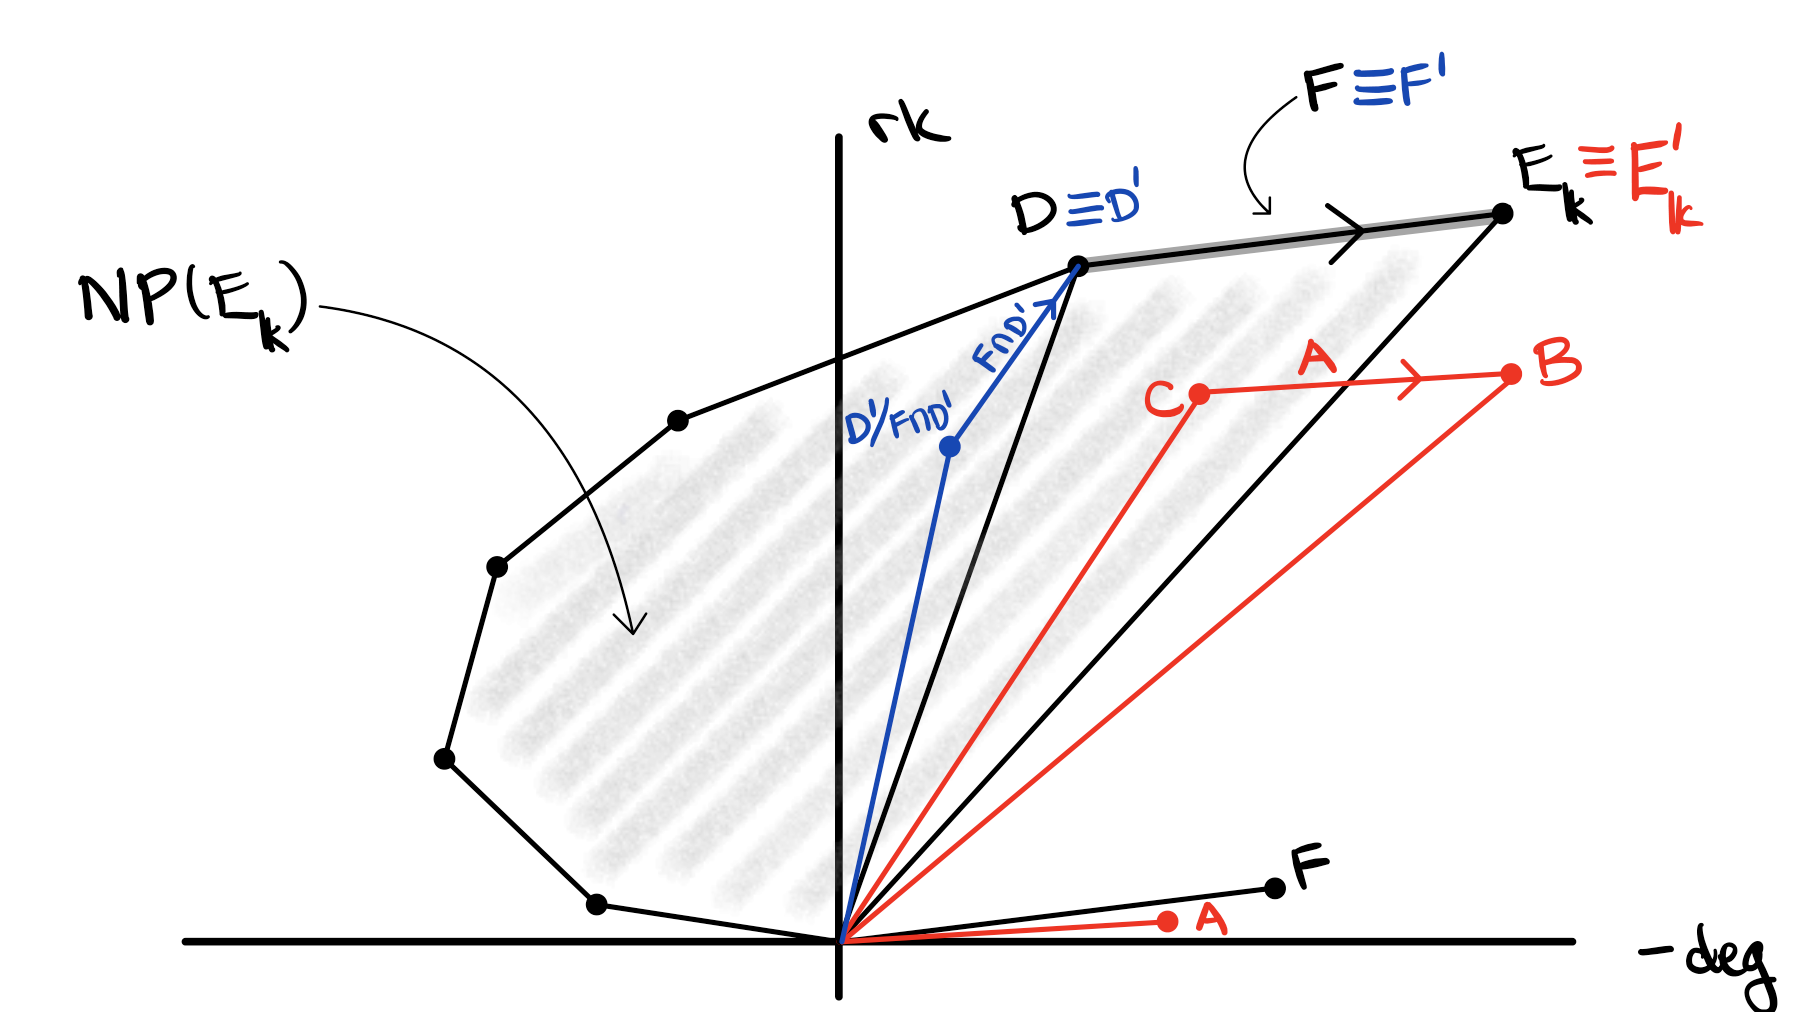
\includegraphics[width=0.76\textwidth]{figures/ch09-langton-polygon.png}
\bookfigurehref{9.3.3}
\caption{$E_{\Bbbk}$ 的 Harder--Narasimhan 多边形 $\operatorname{HNP}(E_{\Bbbk})$ 以灰色表示. 红色 (分别地, 蓝色) 向量用于说明包含关系 $\operatorname{HNP}(E_{\Bbbk}')\subseteq\operatorname{HNP}(E_{\Bbbk})$ 的证明 (分别地, 等号成立时 \eqref{src:9.3-langton-double-star} 的分裂).}\label{src:9.3.3}
\end{figure}
仿照对 $E_{\Bbbk}$ 构造 \eqref{src:9.3-langton-star} 的过程, 令 $0\to D'\to E_{\Bbbk}'\to F'\to0$ 为取 $D'$ 为 $E_{\Bbbk}'$ 的 Harder--Narasimhan 滤过的最后一项所得的短正合列. 我们断言:
\begin{enumerate}[(i)]
\item $\operatorname{HNP}(E_{\Bbbk}')\subseteq\operatorname{HNP}(E_{\Bbbk})$;
\item 若 $\operatorname{HNP}(E_{\Bbbk}')=\operatorname{HNP}(E_{\Bbbk})$, 则复合 $F\to E_{\Bbbk}'\to F'$ 和 $D'\to E_{\Bbbk}'\to D$ 为同构. 特别地, \eqref{src:9.3-langton-double-star} 分裂.
\end{enumerate}
对 (i), 子层 $B\subseteq E_{\Bbbk}'$ 诱导短正合列的交换图
\[
\begin{tikzcd}[ampersand replacement=\&,column sep=small]
0\arrow[r]\&A\arrow[r]\arrow[d]\&B\arrow[r]\arrow[d]\&C\arrow[r]\arrow[d]\&0\\
0\arrow[r]\&F\arrow[r]\&E_{\Bbbk}'\arrow[r]\&D\arrow[r]\&0.
\end{tikzcd}
\]
因为 $C\subseteq D\subseteq E_{\Bbbk}$, 有 $\mu(C)\leq d/r$ 或 $Z(C)\in\operatorname{HNP}(E_{\Bbbk})$. 因为 $F$ 半稳定, 若 $A\ne0$, 则 $\mu(A)\leq\mu(F)$. 利用 $Z(B)=Z(A)+Z(C)$, 这两个事实蕴含 $\mu(B)\leq d/r$ 或 $Z(B)\in\operatorname{HNP}(E_{\Bbbk})$.

对 (ii), 有短正合列 $0\to D'\to E_{\Bbbk}'\to F'\to0$, 满足 $Z(F')=Z(F)$. 复合 $F\to E_{\Bbbk}'\to F'$ 的核为 $D'\cap F$, 它处于短正合列
\[
0\to F\cap D'\to D'\to D'/F\cap D'\to0
\]
中. 假设 $F\cap D'\ne0$, 则 $F$ 的半稳定性以及 $F=E_{\Bbbk}/D$ 和 $D'\subseteq E_{\Bbbk}'$ 的构造给出不等式
\[
\mu(F\cap D')\leq\mu(F)<\mu(E_{\Bbbk})=\mu(E_{\Bbbk}')<\mu(D'),
\]
从而蕴含 $\mu(D'/F\cap D')>\mu(D')$. 因为 $D'/F\cap D'\subseteq D\subseteq E_{\Bbbk}$, $Z(D'/F\cap D')\in\operatorname{HNP}(E_{\Bbbk})$ 位于 $Z(D')$ 的左侧. 但这蕴含 $\mu(F\cap D')>\mu(F)$, 与 $F$ 的半稳定性矛盾. 所以 $F\cap D'=0$, $F\to E_{\Bbbk}'\to F'$ 单射. 因为 $F,F'$ 的次数与秩相同, $F\to F'$ 是同构, 使 \eqref{src:9.3-langton-double-star} 分裂.

由于包含于 $\operatorname{HNP}(E_{\Bbbk})$ 的 Harder--Narasimhan 多边形只有有限个, 归纳地用 $E'$ 替换 $E$ 并应用断言 (i), 要么得到延伸 $E^*$ 的半稳定向量丛族, 要么得到无限族 $\cdots\subseteq E^{(2)}\subseteq E^{(1)}\subseteq E^{(0)}$, 其中每个 $E^{(n)}$ 都有相同的 Harder--Narasimhan 多边形. 我们将说明后一情形导致矛盾. 由断言 (ii), 每个 $E_{\Bbbk}^{(n)}\cong D\oplus F$ 分裂. 用 $E^{(0)}$ 替换 $E$ 后, 留给读者验证: $C_{R/\mathfrak m^n}$ 上的层 $E/E^{(n)}$ 在 $R/\mathfrak m^n$ 上平坦, 且 $(E/E^{(n+1)})\otimes_{R/\mathfrak m^{n+1}}R/\mathfrak m^n\cong E/E^{(n)}$ (习题~\bookref{9.3.4}). 这蕴含存在相容提升
\[
\begin{tikzcd}[ampersand replacement=\&,column sep=large]
\Spec\Bbbk\arrow[r,"{[E_{\Bbbk}\twoheadrightarrow F]}"]\arrow[d]\&\Quot^{P_F}(E/C_R/R)\arrow[d]\\
\Spec R/\mathfrak m^n\arrow[r]\arrow[ur,dashed,"{[E_{R/\mathfrak m^n}\twoheadrightarrow E/E^{(n)}]}"']\&\Spec R,
\end{tikzcd}
\]
其中 $P_F$ 是 $F$ 的 Hilbert 多项式. 由 Quot 概形的固有性 (命题~\bookref{2.4.2}), 映射 $\Quot^{P_F}(E/C_R/R)\to\Spec R$ 的像闭, 因而满射. 所以存在扩张 $R\to R'$ 和截面 $[E_{R'}\to\widetilde F]:\Spec R'\to\Quot^{P_F}(E/C_R/R)$. (若 $R$ 完备, 则 Grothendieck 存在定理 (\bookref{C.5.3}) 蕴含无需扩张就存在截面.) 限制到 $R'$ 的分式域 $K'$, 得到商 $E_{K'}\to\widetilde F_{K'}$, 满足 $\mu(\widetilde F_{K'})>\mu(E_{K'})$. 这蕴含 $E_{K'}$ 不半稳定. 因为半稳定性不受域扩张影响 (推论~\bookref{9.1.29}), 这与 $E_K$ 的半稳定性矛盾. 另见 \cite{Lan75}, \cite[定理 2.B.1]{HL10} 和 \cite[定理 5.7]{Mar78}.
\end{proof}
\begin{exercise}\label{src:9.3.4}
验证上述证明中省略的细节: $(E/E^{(n+1)})\otimes_{R/\mathfrak m^{n+1}}R/\mathfrak m^n\cong E/E^{(n)}$, 且 $E/E^{(n)}$ 在 $R/\mathfrak m^n$ 上平坦.

\textit{提示:} 先证明 $(E/E^{(n)})_{\Bbbk}\cong F$. 然后利用等同 $E^{(n)}/E^{(n+1)}\cong F\cong(E/E^{(n+1)})_{\Bbbk}\cong E/E^{(n+1)}\otimes_{R/\mathfrak m^{n+1}}\mathfrak m^n$, 将短正合列 $0\to E^{(n)}/E^{(n+1)}\to E/E^{(n+1)}\to E/E^{(n)}\to0$ 与右正合列
\[
\begin{aligned}
E/E^{(n+1)}\otimes_{R/\mathfrak m^{n+1}}\mathfrak m^n\to E/E^{(n+1)}\\
\to E/E^{(n+1)}\otimes_{R/\mathfrak m^{n+1}}R/\mathfrak m^n\to0
\end{aligned}
\]
比较. 对 $n$ 作归纳, 并对 $R/\mathfrak m^{n+1}\to R/\mathfrak m^n$ 应用平坦性的局部判据 (\bookref{A.2.6}), 建立 $E/E^{(n+1)}$ 在 $R/\mathfrak m^{n+1}$ 上的平坦性.
\end{exercise}
\begin{corollary}\label{src:9.3.5}
代数叠 $\cBun_{r,d}^{\mathrm{ss}}(C)$ 在 $\Bbbk$ 上普遍闭.
\end{corollary}
\begin{proof}
由半稳定性的有界性 (\bookref{9.2.8}), $\cBun_{r,d}^{\mathrm{ss}}(C)$ 有限型, 特别地, 拟紧. 因而可应用普遍闭性的赋值判据 (\bookref{4.8.7}).
\end{proof}

\subsection{固有模空间的存在性}\label{src:9.3.2-subsection}
回顾 $\Theta$-完备性和 S-完备性是赋值判据 (定义~\bookref{7.9.10} 和 \bookref{7.9.14}), 它们保证分离良模空间的存在性 (定理~\bookref{7.10.1}). 我们将利用来自 $\Theta$ 的映射与凝聚层滤过之间的解释 (命题~\bookref{7.9.6}), 以及参数化凝聚层的叠 $\Coh(X)$ 是 $\Theta$-完备且 S-完备的事实 (命题~\bookref{7.9.30}), 验证 $\cBun_{r,d}^{\mathrm{ss}}$ 是 $\Theta$-完备且 S-完备的. 后一事实对任意射影概形 $X$ 成立. 为此, 给出 $\Coh(X)$ 的开子叠是 $\Theta$-完备或 S-完备的一般判据. 为表述 S-完备性判据, 需要如下概念: 两个 $\mathbb Z$-分次滤过
\[
E_\bullet:0\subseteq\cdots\subseteq E_{i-1}\subseteq E_i\subseteq E_{i+1}\subseteq\cdots\subseteq E
\]
和
\[
F^\bullet:F\supseteq\cdots\supseteq F^{i-1}\supseteq F^i\supseteq F^{i+1}\supseteq\cdots\supseteq0
\]
称为\newterm{相反的}{opposite}, 若对所有 $i$, 有 $E_i/E_{i-1}\cong F^i/F^{i+1}$. 推广滤过与来自 $\Theta$ 的映射之间的对应, 满足 $i\ll0$ 时 $E_i=0$, $F^i=F$, 且 $i\gg0$ 时 $E_i=E$, $F^i=0$ 的相反滤过 $E_\bullet,F^\bullet$ 的数据, 等价于给出映射
\[
[\Spec(\Bbbk[x,y]/xy)/\mathbb G_m]\to\Coh(X),
\]
其中 $t\cdot(x,y)=(tx,t^{-1}y)$. 此时该映射将 $(1,0)$ 映到 $E$, 将 $(0,1)$ 映到 $F$, 将 $(0,0)$ 映到 $\operatorname{gr}E_\bullet\cong\operatorname{gr}F^\bullet$.
\begin{proposition}\label{src:9.3.6}
设 $X$ 是代数闭域 $\Bbbk$ 上的射影概形, $\mathcal U\subseteq\Coh(X)$ 是开子叠.
\begin{enumerate}[(1)]
\item 子叠 $\mathcal U$ 是 $\Theta$-完备的, 当且仅当对每个 DVR $R$ (分式域为 $K$, 剩余域为 $\kappa$), 每个 $X_R$ 上在 $R$ 上平坦的凝聚层 $\mathcal E$, 以及每个满足 $i\ll0$ 时 $\mathcal E_i=0$, $i\gg0$ 时 $\mathcal E_i=\mathcal E$, 且每个 $\mathcal E_i/\mathcal E_{i-1}$ 在 $R$ 上平坦的 $\mathbb Z$-分次滤过 $\mathcal E_\bullet$, 若 $\mathcal E$ 和 $\operatorname{gr}(\mathcal E_\bullet|_K)$ 在 $\mathcal U$ 中, 则 $\operatorname{gr}(\mathcal E_\bullet|_\kappa)$ 也必须在 $\mathcal U$ 中.
\item 若对每个域扩张 $\kappa/\Bbbk$ 以及 $E,F\in\mathcal U(\kappa)$ 的每对相反滤过 $E_\bullet,F^\bullet$, 伴随分次 $\operatorname{gr}E_\bullet$ 在 $\mathcal U(\kappa)$ 中, 则子叠 S-完备.
\end{enumerate}
\end{proposition}
\begin{proof}
因为已知 $\Coh(X)$ 是 $\Theta$-完备且 S-完备的 (命题~\bookref{7.9.30}), $\mathcal U$ 的赋值判据等价于对所有如下交换图存在提升:
\[
\begin{tikzcd}[ampersand replacement=\&,column sep=small]
\Theta_R\setminus0\arrow[r]\arrow[d,hook]\&\mathcal U\arrow[d,hook]\&\Phi_R\setminus0\arrow[r]\arrow[d,hook]\&\mathcal U\arrow[d,hook]\\
\Theta_R\arrow[r]\arrow[ur,dashed]\&\Coh(X)\&\Phi_R\arrow[r]\arrow[ur,dashed]\&\Coh(X),
\end{tikzcd}
\]
其中 $R$ 是 DVR. 换言之, 需说明在唯一的填充 $\Theta_R\to\Coh(X)$ 和 $\Phi_R\to\Coh(X)$ 下, $0$ 的像包含于 $\mathcal U$. 由命题~\bookref{7.9.6}, 映射 $\Theta_R\to\Coh(X)$ 由 $C_R$ 上在 $R$ 上平坦的凝聚层 $\mathcal E$, 及满足 $i\ll0$ 时 $\mathcal E_i=0$, $i\gg0$ 时 $\mathcal E_i=\mathcal E$, 且每个 $\mathcal E_i/\mathcal E_{i-1}$ 在 $R$ 上平坦的 $\mathbb Z$-分次滤过 $\mathcal E_\bullet$ 分类. 此外, 限制 $\Theta_R\setminus0\to\Coh(X)$ 经过 $\mathcal U$ 分解, 当且仅当 $\mathcal E$ 和 $\operatorname{gr}(\mathcal E_\bullet|_K)$ 在 $\mathcal U$ 中. 因为 $0$ 在 $\Theta_R\to\Coh(X)$ 下的像为 $\operatorname{gr}(\mathcal E_\bullet|_\kappa)$, 得到 (1).

对 (2), 将 $\Phi_R\to\Coh(X)$ 沿 $\pi=0$ 限制, 得到对应于相反滤过 $E_\bullet,F^\bullet$ 的映射 $[\Spec(\kappa[x,y]/xy)/\mathbb G_m]\to\Coh(X)$. 若 $\operatorname{gr}E_\bullet$ 在 $\mathcal U$ 中, 则 $\Phi_R\to\Coh(X)$ 的像包含于 $\mathcal U$. 另见 \cite[命题 3.17]{WZ25}.
\end{proof}
虽然后文不需要, 下述习题在概念上有帮助.
\begin{exercise}\label{src:9.3.7}
证明当 $X=C$ 是曲线时, 命题~\bookref{9.3.6}(2) 的逆命题成立.

\textit{提示:} 令 $\mathcal X_0:=[\Spec(\Bbbk[x,y]/xy)/\mathbb G_m]\subset\Phi_R$, $\mathcal X_n$ 为其幂零加厚. 利用形变理论, 将映射 $\mathcal X_0\to\Coh(C)$ 延拓为相容映射 $\mathcal X_n\to\Coh(C)$, 再利用凝聚 Tannaka 对偶 (\bookref{7.6.9}) 进一步延拓为映射 $\Phi_R\to\Coh(C)$.
\end{exercise}
\begin{proposition}\label{src:9.3.8}
对代数闭域 $\Bbbk$ 上的光滑连通射影曲线 $C$, 代数叠 $\cBun_{r,d}^{\mathrm{ss}}$ 是 $\Theta$-完备且 S-完备的.
\end{proposition}
\begin{proof}
应用命题~\bookref{9.3.6} 建立这两种性质. 对 $\Theta$-完备性, 设 $\mathcal E$ 是 $C_R$ 上在 $R$ 上平坦的凝聚层, $\mathcal E_\bullet$ 是 $\mathbb Z$-分次滤过, 满足 $i\ll0$ 时 $\mathcal E_i=0$, $i\gg0$ 时 $\mathcal E_i=\mathcal E$, 且每个 $\mathcal E_i/\mathcal E_{i-1}$ 在 $R$ 上平坦. 假设 $\mathcal E$ 和 $\operatorname{gr}(\mathcal E_\bullet|_K)$ 在 $\cBun_{r,d}^{\mathrm{ss}}$ 中. 因为次数与秩在平坦族中不变, $\operatorname{gr}(\mathcal E_\bullet|_\kappa)\in\Coh_{r,d}$. 为说明 $\operatorname{gr}(\mathcal E_\bullet|_\kappa)$ 半稳定, 只需说明每个因子 $(\mathcal E_i/\mathcal E_{i-1})_\kappa$ 半稳定且斜率为 $d/r$. 因为 $(\mathcal E_i)_\kappa\subseteq\mathcal E_\kappa$ 是半稳定层中斜率相同的子层, 每个 $(\mathcal E_i)_\kappa$ 半稳定. 由于固定斜率的半稳定层组成 Abel 范畴 (习题~\bookref{9.1.17}), $(\mathcal E_i/\mathcal E_{i-1})_\kappa=(\mathcal E_i)_\kappa/(\mathcal E_{i-1})_\kappa$ 半稳定且斜率为 $d/r$.

对 S-完备性, 设
\[
\begin{aligned}
E_\bullet&:\cdots\subseteq E_{i-1}\subseteq E_i\subseteq\cdots\subseteq E,\\
F^\bullet&:F\supseteq\cdots\supseteq F^i\supseteq F^{i+1}\supseteq\cdots
\end{aligned}
\]
是域扩张 $\kappa/\Bbbk$ 上 $C_\kappa$ 上半稳定向量丛 $E,F$ 的相反滤过. 这意味着 $E_i/E_{i-1}\cong F^i/F^{i+1}$. 归纳证明每个 $E_i,F^i$ 半稳定且斜率为 $d/r$. 由习题~\bookref{9.1.17}, 这建立所需的 $\operatorname{gr}E_\bullet=\bigoplus E_i/E_{i-1}$ 的半稳定性. 因为 $i\ll0$ 时 $E_i=0$, $F_i=F$, 且 $F$ 半稳定, $i\ll0$ 时 $E_j,F_j$ 半稳定. 假设 $j\leq i$ 时 $E_j,F_j$ 半稳定. 因为 $F_{i+1}\cong\ker(F_i\to E_i/E_{i-1})$ 是同斜率半稳定向量丛之间映射的核, $F_{i+1}$ 半稳定且斜率为 $d/r$. 另一方面, $E_{i+1}/E_i\cong F_{i+1}/F_{i+2}$ 既是半稳定向量丛 $E/E_i$ 的子层 (利用 $E$ 的半稳定性和归纳假设), 又是半稳定向量丛 $F_{i+1}$ 的商. 所以 $\mu(E_{i+1}/E_i)=d/r$, 从而 $E_{i+1}$ 半稳定且斜率为 $d/r$.
\end{proof}
向量丛叠 $\cBun_{r,d}$ 则既不 $\Theta$-完备, 也不 S-完备.
\begin{example}\label{src:9.3.9}
设 $g\geq2$. 令 $p\in C(\Bbbk)$ 为截面 $s\in\Gamma(C,\mathcal O(p))$ 的零点, $I\subseteq\mathcal O_{C_R}$ 为 $(p,0)\in C\times\Spec R$ 的理想层. 单射 $(s,-\pi):\mathcal O_{C_R}(-p)\hookrightarrow\mathcal O_{C_R}\oplus\mathcal O_{C_R}(-p)$ 的商为 $I$, 它无挠, 因而在 $R$ 上平坦, 但不是向量丛. 由命题~\bookref{9.3.6}, $\cBun_{2,-1}$ 不 $\Theta$-完备.

设 $L,M$ 为 $C$ 上线丛, $p\in C(\Bbbk)$ 是使 $\operatorname{Ext}_{\mathcal O_C}^1(M,L(p))$ 和 $\operatorname{Ext}_{\mathcal O_C}^1(L,M(p))$ 非零的点; 若 $L,M$ 次数相同, Riemann--Roch 计算说明这两个 $\operatorname{Ext}^1$ 群都非零. 令 $Q$ (分别地, $Q'$) 是 $M$ 被 $L(p)$ (分别地, $L$ 被 $M(p)$) 的非平凡扩张. 则
\[
E_\bullet:0\subseteq L\subseteq L(p)\subseteq Q
\quad\text{和}\quad F^\bullet:Q'\supseteq M(p)\supseteq M\supseteq0
\]
定义相反滤过, 其中 $E_0=L$, $F^0=Q'$. 伴随分次 $\operatorname{gr}E_\bullet=L\oplus\kappa(p)\oplus M$ 不是向量丛. 由命题~\bookref{9.3.6}, $\cBun_{1,d}$ 不 S-完备, 其中 $d=\deg L+\deg M+1$.
\end{example}
\begin{exercise}\label{src:9.3.10}
证明 $\cBun_{r,d}^{\mathrm{simple}}$ 不 S-完备, 并推出 $M_{r,d}^{\mathrm{simple}}$ 不分离. (由习题~\bookref{9.2.25}, $\cBun_{r,d}^{\mathrm{simple}}$ 和 $M_{r,d}^{\mathrm{simple}}$ 在 $\Bbbk$ 上都不是有限型的.)
\end{exercise}
\begin{theorem}\label{src:9.3.11}
设 $C$ 是特征为 $0$ 的代数闭域 $\Bbbk$ 上的光滑连通射影曲线. 对每个 $r>0$ 和 $d$, 存在 Cartesian 图
\[
\begin{tikzcd}[ampersand replacement=\&]
\cBun_{r,d}^{\mathrm s}\arrow[r]\arrow[d]\&\cBun_{r,d}^{\mathrm{ss}}\arrow[d]\\
M_{r,d}^{\mathrm s}\arrow[r]\&M_{r,d}^{\mathrm{ps}},
\end{tikzcd}
\]
其中 $M_{r,d}^{\mathrm{ps}}$ 是 $\Bbbk$ 上的固有代数空间, $\cBun_{r,d}^{\mathrm{ss}}\to M_{r,d}^{\mathrm{ps}}$ 是良模空间, $\cBun_{r,d}^{\mathrm s}\to M_{r,d}^{\mathrm s}$ 是带 $\mathbb G_m$-带的 gerbe. 此外,
\[
\dim M_{r,d}^{\mathrm{ps}}=\dim\cBun_{r,d}^{\mathrm{ss}}+1=r^2(g-1)+1.
\]
\end{theorem}
\begin{proof}
由半稳定性的有界性 (\bookref{9.2.8}), $M_{r,d}^{\mathrm{ps}}$ 有限型, 且它是 $\Theta$-完备且 S-完备的 (命题~\bookref{9.3.8}); 因而分离代数空间 $\pi:\cBun_{r,d}^{\mathrm{ss}}\to M_{r,d}^{\mathrm{ps}}$ 的存在性直接来自良模空间存在定理 (\bookref{7.10.1}). 由于 $\cBun_{r,d}^{\mathrm{ss}}$ 由 Langton 定理 (\bookref{9.3.5}) 普遍闭, $M_{r,d}^{\mathrm{ps}}$ 固有.

因为每个稳定丛多重稳定, 从而由命题~\bookref{9.1.35} 为 $\cBun_{r,d}^{\mathrm{ss}}$ 的闭点, 得到 $\pi^{-1}(\pi(\cBun_{r,d}^{\mathrm s}))=\cBun_{r,d}^{\mathrm s}$. 由于 $\pi$ 普遍闭, $\pi(\cBun_{r,d}^{\mathrm s})\subseteq M_{r,d}^{\mathrm{ps}}$ 开. 另一方面, 推论~\bookref{9.2.26} 给出带 $\mathbb G_m$-带的 gerbe $\cBun_{r,d}^{\mathrm s}\to M_{r,d}^{\mathrm s}$ 的存在性. 良模空间与带 $\mathbb G_m$-带的 gerbe 都对到代数空间的映射万有, 因而 $M_{r,d}^{\mathrm s}\cong\pi(\cBun_{r,d}^{\mathrm s})$.

为计算维数, 使用 $M_{r,d}^{\mathrm s}\subseteq M_{r,d}^{\mathrm{ps}}$ 开且稠密; 这来自 $\cBun_{r,d}^{\mathrm s}\subseteq\cBun_{r,d}$ 开且稠密的事实 (定理~\bookref{9.2.16}). 因为 $\cBun^{\mathrm s}\to M_{r,d}^{\mathrm s}$ 是带 $\mathbb G_m$-带的 gerbe, 且 $\dim B\mathbb G_m=-1$, 得到
\[
\dim M_{r,d}^{\mathrm{ps}}=\dim M_{r,d}^{\mathrm s}
=\dim\cBun_{r,d}^{\mathrm s}+1=r^2(g-1)+1,
\]
其中利用了命题~\bookref{4.7.9} 对 $\cBun_{r,d}$ 维数的计算.
\end{proof}
\begin{exercise}\label{src:9.3.12}
对每个 $\xi\in\mathrm{Pic}(C)$, 以 $\cBun_{r,\xi}^{\mathrm{ss}}$ (分别地, $\cBun_{r,\xi}^{\mathrm s}$) 表示模叠 $\cBun_{r,\xi}$ 中参数化行列式为 $\xi$ 的半稳定 (分别地, 稳定) 向量丛的子叠 (定义~\bookref{9.2.27}). 证明 $\cBun_{r,\xi}^{\mathrm{ss}}$ 是 $\Theta$-完备且 S-完备的. 推出在特征 $0$ 下存在固有良模空间 $\cBun_{r,\xi}^{\mathrm{ss}}\to M_{r,\xi}^{\mathrm{ps}}$, 限制为 $\mu_r$-gerbe $\cBun_{r,\xi}^{\mathrm s}\to M_{r,\xi}^{\mathrm s}$, 且 $M_{r,\xi}^{\mathrm s}\subseteq M_{r,\xi}^{\mathrm{ps}}$ 为开子空间.

\textit{提示:} 利用 $\cBun_{r,\xi}^{\mathrm{ss}}\to\cBun_{r,\deg\xi}^{\mathrm{ss}}$ 仿射.
\end{exercise}
\begin{exercise}\label{src:9.3.13}
证明存在交换图
\[
\begin{tikzcd}[ampersand replacement=\&]
\cBun_{r,d}^{\mathrm{ss}}\arrow[r,"\det"]\arrow[d]\&\underline{\mathcal P\!ic}^d\arrow[d]\\
M_{r,d}^{\mathrm{ps}}\arrow[r,"\det"']\&\underline{\mathrm{Pic}}^d,
\end{tikzcd}
\]
其中 $\underline{\mathcal P\!ic}^d$ 和 $\underline{\mathrm{Pic}}^d$ 为 Picard 叠与 Picard 概形 (见 \S\bookref{7.4.8-subsection}). 对次数为 $d$ 的线丛 $\xi$, 证明 $M_{r,d}^{\mathrm{ps}}\to\underline{\mathrm{Pic}}^d$ 在 $\xi$ 上的纤维与 $M_{r,\xi}^{\mathrm{ps}}$ 等同.
\end{exercise}
注意 $\cBun_{r,d}^{\mathrm{ss}}(C)$ (同样也包括 $\cBun_{r,\xi}^{\mathrm{ss}}(C)$) 的每个闭点都有约化自同构群; 这可由 $\cBun_{r,d}^{\mathrm{ss}}(C)$ 的 S-完备性和命题~\bookref{7.10.30} 得到, 也可在特征 $0$ 下由良模空间的存在性和习题~\bookref{7.5.27} 得到. 因为 $\cBun_{r,d}^{\mathrm{ss}}(C)$ 的闭点对应于多重稳定向量丛 (这一事实一般成立, 但命题~\bookref{9.1.35} 仅在特征 $0$ 下证明), 再次得到多重稳定向量丛具有约化自同构群这一事实, 我们在推论~\bookref{9.1.16} 中已直接建立它. 严格半稳定但非多重稳定的向量丛则可能具有非约化自同构群.
\begin{exercise}\label{src:9.3.14}
构造具有非约化自同构群的半稳定向量丛.

\textit{提示:} 考虑稳定向量丛的非分裂扩张.
\end{exercise}

\subsection{不稳定轨迹的分层}\label{src:9.3.3-subsection}
凝聚层的模叠 $\Coh_{r,d}$ 有以 Harder--Narasimhan 多边形为指标的局部闭子叠分层. 此分层称为\newterm{Harder--Narasimhan 分层}{Harder--Narasimhan stratification} 或\newterm{Shatz 分层}{Shatz stratification}. 它最早在 \cite{Sha77} 中证明, 与本章大多数其他结果 (例如 Harder--Narasimhan 滤过及 Langton 定理) 一样, 可推广到任意维射影簇上的无挠层.

回顾对 $C$ 上凝聚层 $F$, Harder--Narasimhan (HN) 多边形 $\operatorname{HNP}(F)\subseteq\mathbb C$ 是当 $E\subseteq F$ 遍历所有不稳定化子层 (即 $\mu(E)\geq\mu(F)$, 等价地, $\arg Z(E)\geq\arg Z(F)$) 时, 点 $Z(E)=-\deg(E)+\operatorname{rk}(E)i$ 的凸包; 见图~\bookref{9.1.25}. 若 $0=F_0\subseteq F_1\subseteq\cdots\subseteq F_l=F$ 是 Harder--Narasimhan 滤过 (\bookref{9.1.21}), 则 $Z(F_i)$ 是 $\operatorname{HNP}(F)$ 的极端点 (推论~\bookref{9.1.26}). HN 多边形由因子 $F_i/F_{i-1}$ 的秩次数对序列确定. 我们使用由包含关系给出的 HN 多边形的偏序. 注意若 $F$ 半稳定, 则 $\operatorname{HNP}(F)$ 为从 $0$ 到 $Z(F)$ 的直线; 若 $F$ 为挠层, 则 $\operatorname{HNP}(F)$ 为顶点 $(0,0),(-\deg F,0),Z(F)$ 构成的多边形.
\begin{theorem}[Harder--Narasimhan/Shatz 分层]\label{src:9.3.15}
设 $C$ 是代数闭域 $\Bbbk$ 上亏格 $g\geq2$ 的光滑连通射影曲线. 存在分层
\[
\Coh_{r,d}=\coprod_{\text{HN 多边形 }\mathcal P}\Coh_{r,d}^{\mathcal P},
\]
其中 $\Coh_{r,d}^{\mathcal P}\subseteq\Coh_{r,d}$ 为局部闭子叠, 对 $C$ 上秩为 $r$, 次数为 $d$ 的向量丛 $E$, 有
\[
E\in\Coh_{r,d}^{\mathcal P}\iff\operatorname{HNP}(E)=\mathcal P.
\]
此外, 对每个 HN 多边形 $\mathcal P$:
\begin{enumerate}[(1)]
\item 设 $S$ 是 $\Bbbk$-概形, $\mathcal F$ 是 $C_S$ 上秩为 $r$, 次数为 $d$ 的向量丛族.
\begin{enumerate}[(a)]
\item 分类 $\mathcal F$ 的映射 $S\to\Coh_{r,d}$ 经过 $\Coh_{r,d}^{\mathcal P}$ 分解, 当且仅当存在向量丛滤过
\[
0=\mathcal F_0\subseteq\mathcal F_1\subseteq\cdots\subseteq\mathcal F_l=\mathcal F,
\]
其因子 $\mathcal F_i/\mathcal F_{i-1}$ 为向量丛, 对每个 $s\in S$, 有 $\operatorname{HNP}(\mathcal F_s)=\mathcal P$, 且 $0=\mathcal F_{0,s}\subseteq\mathcal F_{1,s}\subseteq\cdots\subseteq\mathcal F_{l,s}=\mathcal F_s$ 是 $\mathcal F_s$ 的 Harder--Narasimhan 滤过.
\item 若 $s\leadsto s_0$ 为特殊化, 则 $\operatorname{HNP}(\mathcal F_s)\subseteq\operatorname{HNP}(\mathcal F_{s_0})$; 换言之, $\Coh_{r,d}^{\mathcal P}$ 的闭包包含于 $\coprod_{\mathcal P'\supseteq\mathcal P}\Coh_{r,d}^{\mathcal P}$.
\end{enumerate}
\item 并集
\[
\Coh_{r,d}^{\leq\mathcal P}:=\bigcup_{\mathcal P'\subseteq\mathcal P}\Coh_{r,d}^{\mathcal P'}
\]
为 $\Coh_{r,d}$ 的开子叠, 而 $\Coh_{r,d}^{\mathcal P}\subseteq\Coh_{r,d}^{\leq\mathcal P}$ 为闭子叠.
\item 以 $e_1,\ldots,e_l\in\mathbb C$ 表示按虚部递增排列的 $\mathcal P$ 的极端点, 以 $P_1,\ldots,P_l$ 表示满足 $Z(G_i)=e_i-e_{i-1}$ 的向量丛 $G_i$ 的 Hilbert 多项式, 则有等同
\[
\Coh_{r,d}^{\mathcal P}\cong
\operatorname{Flag}^{P_1,\ldots,P_l}(\mathcal F_{\mathrm{univ}}/C\times\Coh_{r,d}^{\leq\mathcal P}/\Coh_{r,d}^{\leq\mathcal P}),
\]
其中右端为 $\Coh_{r,d}^{\leq\mathcal P}$ 上的 Flag 概形 (习题~\bookref{2.4.7}), 参数化万有丛 $\mathcal F_{\mathrm{univ}}$ 的滤过 $\mathcal F_\bullet$, 第 $i$ 个因子 $\mathcal F_i/\mathcal F_{i-1}$ 的 Hilbert 多项式为 $P_i$.
\end{enumerate}
\end{theorem}
\begin{remark}\label{src:9.3.16}
当 $\mathcal P$ 为从 $0$ 到 $Z(F)$ 的直线时, $\Coh_{r,d}^{\mathcal P}=\cBun_{r,d}^{\mathrm{ss}}$ 是半稳定轨迹.
\end{remark}
\begin{proof}
先证明对 $\Bbbk$-概形 $S$ 以及 $C_S$ 上在 $S$ 上平坦的秩 $r$, 次数 $d$ 凝聚层 $\mathcal F$, 存在分层
\[
S=\coprod_{\mathcal P}S_{\mathcal P},
\]
分为局部闭子概形 $S_{\mathcal P}\subseteq S$, 用 $S_{\mathcal P}$ 替换 $\Coh_{r,d}^{\mathcal P}$ 后, 性质 (1)--(3) 成立; 当 $S$ 为 Noether 时分层有限. 由极限方法 (\bookref{B.3}), 可假设 $S$ 为 Noether.

纤维 $\mathcal F_s$ 的 Harder--Narasimhan 多边形只有有限种可能的 $\mathcal P$, 因为纤维子层的次数上有界 (习题~\bookref{9.1.28}). 其次, 对每个这样的多边形 $\mathcal P$, 其极端顶点有 Hilbert 多项式 $P_1,\ldots,P_l$ (沿用 (3) 的记号), 存在 $S$ 上固有的 Flag 概形 $\operatorname{Flag}^{P_1,\ldots,P_l}(\mathcal F/C_S/S)$. 将其闭像记为
\[
S_{\geq\mathcal P}:=\im(\operatorname{Flag}^{P_1,\ldots,P_l}(\mathcal F/C_S/S)\to S).
\]
点 $s\in S$ 位于 $S_{\geq\mathcal P}$, 当且仅当 $\mathcal F_s$ 有伴随多边形为 $\mathcal P$ 的滤过. 则
\[
S_{\mathcal P}:=S_{\geq\mathcal P}\setminus\bigcup_{\mathcal P'\supsetneq\mathcal P}S_{\geq\mathcal P'}
\]
为 $S_{\geq\mathcal P}$ 的开子叠. 因为 Harder--Narasimhan 多边形包含每个不稳定化子层 (推论~\bookref{9.1.26}), 点 $s\in S$ 位于 $S_{\mathcal P}$ 当且仅当 $\operatorname{HNP}(\mathcal F_s)=\mathcal P$. 除 $S_{\mathcal P}$ 的函子性外, 这给出 (1)(a).

为证明 (1)(b), 设 $\Spec R\to S$ 为表示特殊化的来自 DVR 的映射. 由于 Harder--Narasimhan 滤过在域扩张下保持不变, 只需证明 $\operatorname{HNP}(\mathcal F_K)\subseteq\operatorname{HNP}(\mathcal F_\kappa)$, 其中 $K,\kappa$ 为 $R$ 的分式域与剩余域. 由 Quot 概形的赋值判据 (命题~\bookref{2.4.2}), $\mathcal F_K$ 的 Harder--Narasimhan 滤过延拓为 $\mathcal F_R$ 的滤过, 再限制为 $\mathcal F_\kappa$ 的滤过. 因为 $\mathcal F_\kappa$ 的此滤过的每一项都位于 $\operatorname{HNP}(\mathcal F_\kappa)$ 中, 有 $\operatorname{HNP}(\mathcal F_K)\subseteq\operatorname{HNP}(\mathcal F_\kappa)$. 由于 $S_{\leq\mathcal P}:=\bigcup_{\mathcal P'\subseteq\mathcal P}S_{\mathcal P'}$ 可构造且在一般化下稳定, 它是开的, 从而建立 (2).

剩下需证明 (2) 以及概形结构 $S_{\mathcal P}\subseteq S$ 对 $S$ 函子性; 只需证明
\[
S_{\mathcal P}\cong\operatorname{Flag}^{P_1,\ldots,P_l}(\mathcal F/C\times S_{\leq\mathcal P}/S_{\leq\mathcal P}).
\]
换言之, 需证明固有态射
\[
\operatorname{Flag}^{P_1,\ldots,P_l}(\mathcal F/C\times S_{\leq\mathcal P}/S_{\leq\mathcal P})\to S_{\leq\mathcal P}
\]
是同构地映到 $S_{\mathcal P}$ 的闭浸入. 为此, 只需说明它在切空间上单射, 即相对切空间为零. 可将上述映射分解为复合
\[
\begin{aligned}
&\operatorname{Flag}^{P_1,\ldots,P_l}(\mathcal F/C\times S_{\leq\mathcal P}/S_{\leq\mathcal P})\\
&\quad\to\operatorname{Flag}^{P_2,\ldots,P_l}(\mathcal F/C\times S_{\leq\mathcal P}/S_{\leq\mathcal P})\to\cdots\\
&\quad\to\Quot^{P_l}(\mathcal F/C\times S_{\leq\mathcal P}/S_{\leq\mathcal P})\to S_{\leq\mathcal P},
\end{aligned}
\]
其中每个态射由相对 Quot 概形给出 (见习题~\bookref{2.4.7}). 分析上述各映射的相对切空间后, 可将单射性断言归约为: 若 $0=\mathcal F_{s,0}\subseteq\mathcal F_{s,1}\subseteq\cdots\subseteq\mathcal F_{s,l}=\mathcal F_s$ 是 $s\in S_{\mathcal P}$ 上纤维 $\mathcal F_s$ 的 Harder--Narasimhan 滤过, $q:\mathcal F_{s,i}\to\mathcal F_{s,i}/\mathcal F_{s,i-1}$ 为第 $i$ 个商, 则 $T_q\Quot^{P_i}(\mathcal F_{s,i}/C_s/\kappa(s))=0$. 由习题~\bookref{2.5.6}, 此切空间与 $\Hom_{\mathcal O_{C_s}}(\mathcal F_{s,i},\mathcal F_{s,i}/\mathcal F_{s,i-1})$ 等同. 因为 $\mathcal F_{s,i}$ 的 Harder--Narasimhan 滤过的每个因子的斜率都严格大于半稳定层 $\mathcal F_{s,i}/\mathcal F_{s,i-1}$ 的斜率, 不存在非平凡同态 (习题~\bookref{9.1.31}). 另见 \cite{Sha77,Nit11}.
\end{proof}
\begin{remark}[相对 Harder--Narasimhan 滤过]\label{src:9.3.17}
由此定理, 对 $C_S$ 上向量丛 $\mathcal F$, 其限制 $\mathcal F_{S_{\mathcal P}}$ 有向量丛滤过 $0=\mathcal F_0\subseteq\mathcal F_1\subseteq\cdots\subseteq\mathcal F_l=\mathcal F_{S_{\mathcal P}}$, 因子 $\mathcal F_i/\mathcal F_{i-1}$ 为向量丛. 对每个 $s\in S_{\mathcal P}$, 此滤过限制为 $C_s$ 上 $\mathcal F_s$ 的 Harder--Narasimhan 滤过, 因而称为\newterm{相对 Harder--Narasimhan 滤过}{relative Harder--Narasimhan filtration}. 取 $\mathcal P$ 为纤维 $\mathcal F_s$ 的 Harder--Narasimhan 多边形中的极小者, 得到开子概形 $U:=S_{\mathcal P}\subseteq S$, 在其上存在相对 Harder--Narasimhan 滤过. 一般而言, 此滤过未必能在 $S$ 上延拓, 但作一次爆破后可以延拓 \cite[定理 2.3.2]{HL10}.
\end{remark}
\begin{remark}[与 HKKN 分层的关系]\label{src:9.3.18}
$\Coh_{r,d}$ 的 Harder--Narasimhan/Shatz 分层与构造模空间 $M_{r,d}^{\mathrm{ps}}$ 的 GIT 设置中的 HKKN 分层一致 \cite{Hos18}.
\end{remark}
\begin{remark}[\texorpdfstring{$\Theta$}{Θ}-分层]\label{src:9.3.19}
$\Coh_{r,d}$ 的 Harder--Narasimhan/Shatz 分层是注记~\bookref{8.7.8} 中定义的 $\Theta$-分层的例子. 对每个 HN 多边形 $\mathcal P$, $\Coh_{r,d}^{\leq\mathcal P}:=\bigcup_{\mathcal P'\leq\mathcal P}\Coh_{r,d}^{\mathcal P'}\subseteq\Coh_{r,d}$ 为开子叠, 并有等同
\[
\begin{aligned}
&\underline{\operatorname{Mor}}([\mathbb A^1/\mathbb G_m],\Coh_{r,d}^{\leq\mathcal P})\\
&\qquad\cong\coprod_{\mathcal P'}\operatorname{Flag}^{\mathcal P'}(\mathcal F_{\mathrm{univ}}/C\times\Coh_{r,d}^{\leq\mathcal P}/\Coh_{r,d}^{\leq\mathcal P}),
\end{aligned}
\]
其中 $\operatorname{Flag}^{\mathcal P'}$ 是上述 (3) 中 $\operatorname{Flag}^{P_1',\ldots,P_l'}$ 的简写; 此事实强化了来自 $[\mathbb A^1/\mathbb G_m]$ 的映射与滤过之间的对应 (命题~\bookref{7.9.6}). 取 $\mathcal P'=\mathcal P$, Flag 概形 $\operatorname{Flag}^{\mathcal P}(\mathcal F_{\mathrm{univ}}/C\times\Coh_{r,d}^{\leq\mathcal P}/\Coh_{r,d}^{\leq\mathcal P})\subseteq\underline{\operatorname{Mor}}([\mathbb A^1/\mathbb G_m],\Coh_{r,d}^{\leq\mathcal P})$ 为连通分支之并, 且由 (3) 定义一个 $\Theta$-层, 即诱导映射 $\operatorname{Flag}^{\mathcal P}(\mathcal F_{\mathrm{univ}}/C\times\Coh_{r,d}^{\leq\mathcal P}/\Coh_{r,d}^{\leq\mathcal P})\to\Coh_{r,d}^{\leq\mathcal P}$ 是同构地映到 $\Coh_{r,d}^{\mathcal P}$ 的闭浸入.

一般地, 若代数叠 $\mathcal X$ 满足固有性的赋值判据的存在性部分, 且 $\mathcal X=\coprod_\lambda\mathcal S_\lambda$ 是 $\Theta$-分层, 则半稳定轨迹 $\mathcal X^{\mathrm{ss}}:=\mathcal X_{\leq0}=\mathcal S_0$ 也满足固有性的赋值判据的存在性部分 \cite[定理 6.5]{AHLH23}. 因而 Langton 定理 (\bookref{9.3.1}) 也可由 $\Coh_{r,d}$ 的 Harder--Narasimhan/Shatz 分层 (\bookref{9.3.15}) 推出.
\end{remark}

% Source printed pp. 476-489 / PDF pp. 484-497.
\section{几何性质}\label{src:9.4}
\begin{epigraph}
有人看见它, 这是奇迹; 另有人谈论它, 这是奇迹; 又有人听见它, 这也是奇迹. 然而即使听过, 也无人真正知晓它.
\epigraphauthor{``薄伽梵歌''}
\end{epigraph}
我们证明半稳定向量丛模叠 $\cBun_{r,d}^{\mathrm{ss}}$, $\cBun_{r,\xi}^{\mathrm{ss}}$ 及其模空间 $M_{r,d}^{\mathrm{ps}}$, $M_{r,\xi}^{\mathrm{ps}}$ 的几何性质: 不可约性 (定理~\bookref{9.4.1}), 单有理性 (定理~\bookref{9.4.2}), 局部阶乘性 (命题~\bookref{9.4.12}), 行列式线丛的性质 (\S\bookref{9.4.3-subsection}), Poincar\'e 丛的刻画 (定理~\bookref{9.4.34}), Picard 群的计算 (定理~\bookref{9.4.36}) 和上同调 (\S\bookref{9.4.6-subsection}). 除 $M_{r,\xi}^{\mathrm{ps}}$ 为 Fano 簇 (推论~\bookref{9.4.43}) 外, 本节的结果与证明不依赖于 $M_{r,d}^{\mathrm{ss}}$ 或 $M_{r,\xi}^{\mathrm{ss}}$ 的射影性.
\subsection{半稳定模叠的不可约性与固定行列式模叠的单有理性}\label{src:9.4.1-subsection}
\begin{theorem}[\texorpdfstring{$\cBun_{r,d}^{\mathrm{ss}}$}{Bunss} 的不可约性]\label{src:9.4.1}
设 $C$ 是代数闭域 $\Bbbk$ 上亏格 $g\geq2$ 的光滑连通射影曲线. 对整数 $r>0$ 和 $d$, $\cBun_{r,d}^{\mathrm{ss}}$ 不可约. 特别地, $M_{r,d}^{\mathrm{ps}}$ 不可约.
\end{theorem}
\begin{theorem}[\texorpdfstring{$\cBun_{r,\xi}^{\mathrm{ss}}$}{Bunss} 的单有理性]\label{src:9.4.2}
设 $C$ 是代数闭域 $\Bbbk$ 上亏格 $g\geq2$ 的光滑连通射影曲线. 对 $r>0$ 和 $\xi\in\mathrm{Pic}(C)$, $\cBun_{r,\xi}^{\mathrm{ss}}$ 不可约且单有理, 即存在支配有理映射 $\mathbb P^N\dashrightarrow\cBun_{r,\xi}^{\mathrm{ss}}$. 特别地, $M_{r,\xi}^{\mathrm{ps}}$ 不可约且单有理.
\end{theorem}
两个定理的关键是下述引理, 它将半稳定向量丛表为其行列式被平凡丛的扩张. 它也是计算 $\operatorname{Pic}(\cBun_{r,d}^{\mathrm{ss}})$ (定理~\bookref{9.4.36}) 的关键. 论证基于 Serre 的思想 (见 \cite[\S2]{Ati57}).
\begin{lemma}\label{src:9.4.3}
$C$ 上每个秩 $r>0$, 次数 $d>r(2g-1)$ 的半稳定向量丛 $F$ 都可写为扩张
\[
0\to\mathcal O_C^{\oplus r-1}\to F\to\det F\to0.
\]
\end{lemma}
\begin{proof}
因为 $\mu(F)>2g-1$, $F$ 由整体截面生成 (引理~\bookref{9.2.7}). 断言对一般的维数 $r-1$ 子空间 $W\subseteq\mathrm H^0(C,F)$, 求值映射
\[
\operatorname{ev}_W:W\otimes\mathcal O_C\hookrightarrow\mathrm H^0(C,F)\otimes\mathcal O_C\twoheadrightarrow F
\]
的余核为线丛. 因而 $\operatorname{ev}_W$ 单射, 检查所诱导的短正合列的行列式可知其余核必为 $\det F$. 用维数计数建立此断言.

可将每个子空间 $W$ 看作 Grassmann 簇 $\Gr(k,\mathrm H^0(C,F))$ 的元素, 其中 $k=\mathrm h^0(C,F)-(r-1)$; 回顾我们约定 Grassmann 簇参数化商 $\mathrm H^0(C,F)\twoheadrightarrow\mathrm H^0(C,F)/W$. 我们将证明
\begin{equation}\label{src:9.4.4}
\{W\mid\operatorname{coker}(\operatorname{ev}_W)\text{ 不是线丛}\}\subseteq\Gr(k,\mathrm H^0(C,F))
\end{equation}
的余维为 $1$ (为什么此轨迹闭?). 求值映射在点 $p\in C(\Bbbk)$ 处的纤维 $\operatorname{ev}_{W,p}:W\to F\otimes\kappa(p)$ 单射, 当且仅当 $\operatorname{coker}(\operatorname{ev}_W)$ 在 $p$ 的某邻域中为线丛. 轨迹
\begin{equation}\label{src:9.4.5}
\{W\mid e_{W,p}\text{ 单射}\}\subseteq\Gr(k,\mathrm H^0(C,F))
\end{equation}
的余维为 $2$ (你知道为什么吗?). 让 $p\in C$ 变化, 推出 \bookeqref{9.4.4} 的余维为 $1$. 另见 \cite[引理 7.1]{DN89} 和 \cite[引理 8.5.3]{LP97}.
\end{proof}
\begin{exercise}[中等]\label{src:9.4.6}
验证省略的细节: 轨迹 \bookeqref{9.4.4} 闭, 轨迹 \bookeqref{9.4.5} 的余维为 $2$.
\end{exercise}
\begin{exercise}[困难, 后文需要]\label{src:9.4.7}
证明 \bookeqref{9.4.4} 是次数为 $d$ 的超曲面.

\textit{提示:} 应用 Porteous 公式 (见 \cite[\S14.4]{Ful98} 或 \cite[\S12.2]{EH16}).
\end{exercise}
\begin{proof}[单有理性 (\bookref{9.4.2}) 的证明]
对 $p\in C(\Bbbk)$, 与 $\mathcal O_C(p)$ 作张量积定义同构 $\cBun_{r,\xi}^{\mathrm{ss}}\to\cBun_{r,\xi(rp)}^{\mathrm{ss}}$. 反复应用此同构后, 可假设 $\deg\xi$ 任意大, 例如大于 $r(2g-1)$. 由习题~\bookref{1.3.22}, 仿射空间 $\underline{\operatorname{Ext}}_{\mathcal O_C}^1(\xi,\mathcal O_C^{\oplus r-1}):=\mathbb A(\operatorname{Ext}_{\mathcal O_C}^1(\xi,\mathcal O_C^{\oplus r-1})^\vee)$ 表示扩张函子. $C\times\underline{\operatorname{Ext}}_{\mathcal O_C}^1(\xi,\mathcal O_C^{\oplus r-1})$ 上的万有扩张 $\mathcal E_{\mathrm{univ}}$ 定义映射
\[
\underline{\operatorname{Ext}}_{\mathcal O_C}^1(\xi,\mathcal O_C^{\oplus r-1})\to\cBun_{r,\xi}.
\]
由引理~\bookref{9.4.3}, 此映射的像包含 $\cBun_{r,\xi}^{\mathrm{ss}}$.
\end{proof}
\begin{remark}[有理性]\label{src:9.4.8}
当 $\gcd(r,d)=1$ 时, 模空间 $M_{r,d}^{\mathrm{ps}}$ 有理; 见 \cite{New75,New80,KS99,Hof10}. 一般情形下有理性仍是未解决的问题.
\end{remark}
\begin{proof}[不可约性 (\bookref{9.4.1}) 的证明]
对点 $p\in C(\Bbbk)$ 反复应用同构 $\cBun_{r,d}^{\mathrm{ss}}\to\cBun_{r,dr}^{\mathrm{ss}}$, $E\mapsto E(p)$, 可假设 $d>r(2g-1)$. 由 $F\mapsto\det F$ 定义的到 Picard 叠的态射 $\cBun_{r,d}^{\mathrm{ss}}\to\underline{\mathcal P\!ic}^d$ 满射, 在 $\xi\in\underline{\mathcal P\!ic}^d(\Bbbk)$ 上的纤维为 $\operatorname{Ext}_{\mathcal O_C}^1(\xi,\mathcal O_C^{\oplus r-1})$ 的开子空间. 因为 $\underline{\mathcal P\!ic}^d$ 和每个纤维都不可约, $\cBun_{r,d}^{\mathrm{ss}}$ 也不可约.
\end{proof}
\begin{exercise}\label{src:9.4.9}
利用单有理性证明中的构造的相对版本, 给出 $\cBun_{r,d}^{\mathrm{ss}}$ 的不可约性的另一种证明. 具体地, 考虑投影 $p_2:C\times\underline{\mathcal P\!ic}^d\to\underline{\mathcal P\!ic}^d$ 及 $C\times\underline{\mathcal P\!ic}^d$ 上的万有线丛 $\xi_{\mathrm{univ}}$, 定义
\[
\mathbb E:=\left(p_{2,*}\mathcal E\!xt_{\mathcal O_{C\times\underline{\mathcal P\!ic}^d}}^1
(\xi_{\mathrm{univ}},\mathcal O_{C\times\underline{\mathcal P\!ic}^d}^{\oplus r-1})\right)^\vee,
\]
并证明万有扩张 (见习题~\bookref{9.2.12}) 定义态射 $\mathbb A(\mathbb E)\to\cBun_{r,d}$, 其像包含半稳定轨迹. 另见 \cite[定理 8.5.2]{LP97}.
\end{exercise}
\subsection{模空间的奇点}\label{src:9.4.2-subsection}
半稳定向量丛模叠 $\cBun_{r,d}^{\mathrm{ss}}$ 和 $\cBun_{r,\xi}^{\mathrm{ss}}$ 光滑. 由良模空间的奇点的一般结果 (\S\bookref{7.5.11-subsection}), 模空间 $M_{r,d}^{\mathrm{ps}}$ 和 $M_{r,\xi}^{\mathrm{ps}}$ 正规, Cohen--Macaulay, 且有有理奇点. 在稳定轨迹上, $\cBun_{r,d}^{\mathrm s}\to M_{r,d}^{\mathrm s}$ 和 $\cBun_{r,\xi}^{\mathrm s}\to M_{r,\xi}^{\mathrm s}$ 分别为带 $\mathbb G_m$-带和 $\boldsymbol\mu_r$-带的 gerbe, 因而 $M_{r,d}^{\mathrm s}$ 与 $M_{r,\xi}^{\mathrm s}$ 也光滑. 特别地, 若 $\gcd(r,d)=1$, 则 $M_{r,d}^{\mathrm{ps}}$ 和 $M_{r,\xi}^{\mathrm{ps}}$ 光滑.

由局部结构定理 (\bookref{7.7.1}) 以及 $\cBun_{r,d}$ 在向量丛 $F$ 处的切空间与 $\operatorname{Ext}_{\mathcal O_C}^1(F,F)$ 的等同, 模叠 $\cBun_{r,d}$ 在 $F$ 处平展局部同构于
\[
[\underline{\operatorname{Ext}}_{\mathcal O_C}^1(F,F)/\underline{\operatorname{Aut}}(F)],
\]
其中 $\underline{\operatorname{Ext}}_{\mathcal O_C}^1(F,F):=\mathbb A(\operatorname{Ext}_{\mathcal O_C}^1(F,F)^\vee)$, 作用为
\[
\alpha\cdot[0\to F\xrightarrow aE\xrightarrow bF\to0]
=[0\to F\xrightarrow{a\circ\alpha^{-1}}E\xrightarrow{\alpha\circ b}F\to0].
\]
若 $F=\bigoplus F_i^{\oplus r_i}$ 多重稳定, $F_i$ 是互不同构的稳定向量丛, 则 $\operatorname{Aut}(F)\cong\prod_i\mathrm{GL}_{r_i}$ 在向量空间
\[
\operatorname{Ext}_{\mathcal O_C}^1(F,F)\cong
\bigoplus_{i,j}\operatorname{Ext}_{\mathcal O_C}^1(F_i,F_j)\otimes\mathrm{Mat}_{r_i,r_j}
\]
上的作用为 $(g_i)\cdot(e_{ij}\otimes M_{ij})=e_{ij}\otimes g_iM_{ij}g_j^{-1}$. 此外, 由良模空间的局部结构定理 (\bookref{7.7.3}), 模空间 $M_{r,d}^{\mathrm{ps}}$ 在多重稳定向量丛 $F$ 处平展局部同构于 $\underline{\operatorname{Ext}}_{\mathcal O_C}^1(F,F)\sslash\underline{\operatorname{Aut}}(F)$. 利用习题~\bookref{9.2.30} 给出的切空间等同, 可类似地描述 $M_{r,\xi}^{\mathrm{ps}}$ 的局部结构.
\begin{exercise}\label{src:9.4.10}
设 $r\geq2$, $\xi$ 为 $C$ 上次数 $d$ 的线丛.
\begin{enumerate}[(a)]
\item 若 $r=g=2$ 且 $d$ 为偶数, 证明 $M_{r,d}^{\mathrm{ps}}$ 和 $M_{r,\xi}^{\mathrm{ps}}$ 光滑.

\textit{提示:} 证明每个局部 GIT 商都与仿射空间等同; 当 $F\cong L\oplus L$ 时, 用例~\bookref{7.5.9} 确定不变量环.
\item 假设 $r\ne2$, $g\ne2$ 或 $d$ 为奇数. 证明 $M_{r,d}^{\mathrm{ps}}$ 和 $M_{r,\xi}^{\mathrm{ps}}$ 的奇点轨迹恰为严格半稳定轨迹的像.
\end{enumerate}
\end{exercise}
\begin{remark}\label{src:9.4.11}
除了上述性质, Narasimhan 与 Ramanan 在 \cite{NR69} 中还对 $g=2$ 时的 $M_{2,\xi}^{\mathrm{ps}}$ 给出显式描述: 若 $d$ 偶, $M_{2,d}^{\mathrm{ps}}\cong\mathbb P^3$; 若 $d$ 奇, $M_{2,d}^{\mathrm{ps}}$ 是 $\mathbb P^5$ 中两个二次超曲面的交. 对任意亏格, \cite{Las96} 描述 $M_{2,\xi}^{\mathrm{ps}}$ 的奇点 (例如重数与切锥).
\end{remark}
\begin{proposition}\label{src:9.4.12}
设 $r>0$ 和 $d$ 为整数, $\xi$ 为 $C$ 上线丛. 模空间 $M_{r,d}^{\mathrm{ps}}$ 和 $M_{r,\xi}^{\mathrm{ps}}$ 局部阶乘.
\end{proposition}
\begin{proof}
$r=g=2$ 时可显式验证 (见习题~\bookref{9.4.10}). 否则, 由习题~\bookref{9.2.18}, 已知 $\operatorname{codim}(\cBun_{r,d}^{\mathrm{ss}}\setminus\cBun_{r,d}^{\mathrm s})\geq2$. 考虑 $\mathbb G_m$-刚性化, 有 Cartesian 图
\[
\begin{tikzcd}[ampersand replacement=\&]
\cBun_{r,d}^{\mathrm s}\!\sslash\mathbb G_m\arrow[r]\arrow[d,"\sim"']\&\cBun_{r,d}^{\mathrm{ss}}\!\sslash\mathbb G_m\arrow[d]\\
M_{r,d}^{\mathrm s}\arrow[r]\&M_{r,d}^{\mathrm{ss}},
\end{tikzcd}
\]
其中左侧竖直映射为同构, 右侧竖直映射为良模空间. 由习题~\bookref{7.5.39}, $M_{r,d}^{\mathrm{ss}}$ 阶乘, 当且仅当 $\cBun_{r,d}^{\mathrm{ss}}\!\sslash\mathbb G_m$ 上每个线丛都下降到 $M_{r,d}^{\mathrm{ss}}$. 后一陈述正是下述引理~\bookref{9.4.13} 的结论. 另见 \cite[定理 A]{DN89}.
\end{proof}
\begin{lemma}\label{src:9.4.13}
设 $L$ 是 $\cBun_{r,d}^{\mathrm{ss}}$ 上线丛. 对每个秩 $r$, 次数 $d$ 的多重稳定向量丛 $F$, $\underline{\operatorname{Aut}}(F)/\mathbb G_m$ 在纤维 $L\otimes\kappa([F])$ 上平凡作用. 特别地, $\operatorname{Pic}(M_{r,d}^{\mathrm{ps}})\cong\operatorname{Pic}(\cBun_{r,d}^{\mathrm{ss}}\!\sslash\mathbb G_m)$.
\end{lemma}
\begin{proof}
令 $k=\gcd(r,d)$, $r'=r/k$, $d'=d/k$. 因为每个 $F_i$ 的斜率为 $d/r$, 可写为 $r_i:=\operatorname{rk}F_i=k_ir'$ 和 $d_i:=\deg F_i=k_id'$, 其中 $k_i$ 为整数. 由于 $(r,d)=\sum_i n_i(\operatorname{rk}F_i,\deg F_i)=\sum_i n_ik_i(r',d')$, 有 $k=\sum_i n_ik_i$. 利用稳定丛的存在性 (\bookref{9.2.16}) 选取稳定丛 $G\in\cBun_{r',d'}^{\mathrm s}$. 则 $G^{\oplus k}$ 是秩为 $r$, 次数为 $d$ 的多重稳定向量丛, 自同构群为 $\mathrm{GL}_k$. 因为 $\mathrm{GL}_k/\mathbb G_m=\mathrm{PGL}_k$ 没有特征标, 它在 $L\otimes\kappa([G^{\oplus k}])$ 上的作用平凡. 为说明对 $F$ 也成立, 考虑态射
\begin{equation}\label{src:9.4.14}
\begin{aligned}
\cBun_{r_1,d_1}^{\mathrm{ss}}\times\cdots\times\cBun_{r_l,d_l}^{\mathrm{ss}}&\to\cBun_{r,d}^{\mathrm{ss}}\\
(E_1,\ldots,E_l)&\mapsto E_1^{\oplus n_1}\oplus\cdots\oplus E_l^{\oplus n_l}.
\end{aligned}
\end{equation}
注意 $F$ 是 $(F_1,\ldots,F_l)$ 的像, $G^{\oplus k}$ 是 $(G^{\oplus k_1},\ldots,G^{\oplus k_l})$ 的像. 有自同构群的包含关系
\[
\operatorname{Aut}(F)\cong\prod_i\mathrm{GL}_{n_i}\subseteq
\prod_i\mathrm{GL}_{n_ik_i}\subseteq\mathrm{GL}_k=\operatorname{Aut}(G^{\oplus k}).
\]
对 \bookeqref{9.4.14} 的像中的每个向量丛 $E=E_1^{\oplus n_1}\oplus\cdots\oplus E_l^{\oplus n_l}$, 有 $\underline{\operatorname{Aut}}(F)/\mathbb G_m\subseteq\operatorname{Aut}(E)/\mathbb G_m$ 在 $L\otimes\kappa([E])$ 上的作用, 从而诱导 $\underline{\operatorname{Aut}}(F)/\mathbb G_m$ 的特征标. 因为特征标离散, 而 $\cBun_{r_1,d_1}^{\mathrm{ss}}\times\cdots\times\cBun_{r_l,d_l}^{\mathrm{ss}}$ 连通, 此特征标必与 $E$ 无关. 取 $E=G^{\oplus k}$, 因为 $\underline{\operatorname{Aut}}(F)/\mathbb G_m$ 在 $L\otimes\kappa([G^{\oplus k}])$ 上的作用平凡, 它在 $L\otimes\kappa([F])$ 上的作用也平凡. 将命题~\bookref{7.5.36} 应用于良模空间 $\cBun_{r,d}^{\mathrm{ss}}\!\sslash\mathbb G_m\to M_{r,d}^{\mathrm{ps}}$, 得到 $\cBun_{r,d}^{\mathrm{ss}}\!\sslash\mathbb G_m$ 上每个线丛都下降为 $M_{r,d}^{\mathrm{ps}}$ 上线丛, 因而 $\operatorname{Pic}(M_{r,d}^{\mathrm{ps}})\cong\operatorname{Pic}(\cBun_{r,d}^{\mathrm{ss}}\!\sslash\mathbb G_m)$.
\end{proof}

\subsection{行列式线丛与广义 \texorpdfstring{$\Theta$}{Θ}-除子}\label{src:9.4.3-subsection}
考虑图
\[
\begin{tikzcd}[ampersand replacement=\&,column sep=large]
V\arrow[d,dash]\&\mathcal F_{\mathrm{univ}}\arrow[d,dash]\&\mathcal L_V\arrow[dd,dash]\\
C\&C\times\cBun_{r,d}\arrow[l,"p_1"']\arrow[dr,"p_2"]\&{}\\
\&{}\&\cBun_{r,d},
\end{tikzcd}
\]
其中 $\mathcal F_{\mathrm{univ}}$ 是 $C\times\cBun_{r,d}$ 上的万有向量丛, $V$ 是 $C$ 上向量丛, $\mathcal L_V$ 是下述定义的 $\cBun_{r,d}$ 上的行列式线丛.
\begin{definition}[行列式线丛]\label{src:9.4.15}
关于 $V$ 的\newterm{行列式线丛}{determinantal line bundle} 定义为 $\cBun_{r,d}$ 上的线丛
\[
\mathcal L_V:=\det\left(\mathrm Rp_{2,*}(\mathcal F_{\mathrm{univ}}\otimes p_1^*V)\right)^\vee.
\]
\end{definition}
\begin{remark}[\texorpdfstring{$\mathcal L_V$}{LV} 良定义]\label{src:9.4.16}
因为投影 $p_2:C\times\cBun_{r,d}\to\cBun_{r,d}$ 可表, 射影且光滑, 相对维数为 $1$, 由上同调与基变换 (\bookref{A.6.2}), 对 $C\times\cBun_{r,d}$ 上每个向量丛 $E$, 导出推前 $\mathrm Rp_{2,*}E$ 是振幅位于 $[0,1]$ 的完美复形. 因而 $\mathrm R^ip_{2,*}E$ 在 $\cBun_{r,d}$ 上光滑局部可计算为向量丛二项复形 $[K^0\to K^1]$ 的上同调. 事实上, 它可整体计算为 $\cBun_{r,d}$ 上向量丛二项复形 $[K^0\to K^1]$ 的上同调; 见 \cite[命题 2.1.10]{HL10}. 无论整体还是光滑局部进行,
\[
\det\mathrm Rp_{2,*}E:=\det(K_0)\otimes\det(K_1)^\vee
\]
都是 $\cBun_{r,d}$ 上良定义的线丛. 关于复形行列式的更一般理论, 另见 \cite{KM76} 和 \cite[Tag 0FJI]{SP}.

取 $E=\mathcal F_{\mathrm{univ}}\otimes p_1^*V$, 可知行列式线丛 $\mathcal L_V$ 良定义. 对 $[F]\in\cBun_{r,d}(\Bbbk)$, 限制 $\mathcal L_V|_{[F]}$ 与 $\det\mathrm H^0(C,F\otimes V)^\vee\otimes\det\mathrm H^1(C,F\otimes V)$ 等同.
\end{remark}
\begin{exercise}[\texorpdfstring{$\mathcal L_V$}{LV} 的性质]\label{src:9.4.17}
\begin{enumerate}[(1)]
\item 证明存在从 $C$ 的 Grothendieck 群出发的群同态
\[
K_0(C)\to\operatorname{Pic}(\cBun_{r,d}),\qquad V\mapsto\mathcal L_V.
\]
特别地, 线丛 $\mathcal L_V$ 的同构类只依赖于 $\operatorname{rk}V$ 和 $\det V$.
\item 若 $V,W$ 是 $C$ 上秩与次数相同的向量丛, 则存在 $\underline{\mathcal P\!ic}^d$ 上的线丛 $\mathcal N$, 使得
\[
\mathcal L_W\cong\mathcal L_V\otimes\det^*\mathcal N,
\]
其中 $\det:\cBun_{r,d}\to\underline{\mathcal P\!ic}^d$ 是将 $F$ 映到 $\det F$ 的映射. 特别地, 对 $\xi\in\mathrm{Pic}(C)$, 行列式线丛 $L_V$ 到 $\cBun_{r,\xi}$ 的限制只依赖于 $V$ 的秩与次数.
\end{enumerate}
(习题~\bookref{9.4.42} 给出 $\mathcal N$ 的显式公式.)
\end{exercise}
\begin{remark}[秩 \texorpdfstring{$r=1$}{r=1} 的情形]\label{src:9.4.18}
取 $r=1$, 得到映射 $\mathrm{Pic}(C)\to\operatorname{Pic}(\underline{\mathcal P\!ic}^d)$, 将线丛 $M$ 映到 $\underline{\mathcal P\!ic}^d$ 上的行列式线丛 $\mathcal P_M$.
\end{remark}
\begin{remark}[\texorpdfstring{$V$}{V} 的数值条件]\label{src:9.4.19}
我们常要求对所有 $[F]\in\cBun_{r,d}(\Bbbk)$, 有 $\chi(C,F\otimes V)=0$, 因为这既使我们能构造 $\mathcal L_V$ 的整体截面, 又使它下降到良模空间. 由 Riemann--Roch 定理 (\bookref{9.1.2}), 此条件等价于
\begin{equation}\label{src:9.4.20}
d\operatorname{rk}(V)+r\deg(V)+r\operatorname{rk}(V)(1-g)=0,
\end{equation}
等价地, $\mu(F)+\mu(V)=g-1$.

令 $r'=r/\gcd(r,d)$, $d'=d/\gcd(r,d)$. 若向量丛 $V$ 对某整数 $m\geq1$ 满足
\[
\operatorname{rk}V=mr'\qquad\text{且}\qquad\deg V=mr'(g-1)-md',
\]
则 $V$ 满足 \bookeqref{9.4.20}.
\end{remark}
\textbf{$\mathcal L_V$ 的截面.} 设 $V$ 是 $C$ 上满足数值条件 \bookeqref{9.4.20} 的向量丛, $[K^0\to K^1]$ 是 $\cBun_{r,d}$ 上计算 $\mathrm Rp_{2,*}(\mathcal F_{\mathrm{univ}}\otimes p_1^*V)$ 的向量丛二项复形. 因为对所有 $[F]\in\cBun_{r,d}(\Bbbk)$, 有 $\chi(C,F\otimes V)=0$, $K^0,K^1$ 的秩相等! 所以
\begin{equation}\label{src:9.4.21}
s_V:\mathcal O_{\cBun_{r,d}}\to\det(K^0)^\vee\otimes\det(K^1)=:\mathcal L_V
\end{equation}
定义 $\mathcal L_V$ 的截面, 有时称为\newterm{$\Theta$-函数}{$\Theta$-function}. 虽然限制 $\mathcal L_V|_{\cBun_{r,\xi}}$ 只依赖于 $\operatorname{rk}V$ 和 $\deg V$ (习题~\bookref{9.4.17}(2)), 截面的限制 $s_V|_{\cBun_{r,\xi}}\in\Gamma(\cBun_{r,\xi},\mathcal L_V|_{\cBun_{r,\xi}})$ 确实依赖于 $V$.
\begin{lemma}\label{src:9.4.22}
截面 $s_V$ 在 $[F]\in\cBun_{r,d}(\Bbbk)$ 处不为零, 当且仅当 $\mathrm H^0(C,F\otimes V)=\mathrm H^1(C,F\otimes V)=0$.
\end{lemma}
\begin{proof}
截面不为零当且仅当 $K^0\otimes\kappa([F])\to K^1\otimes\kappa([F])$ 是同构, 这等价于 $F\otimes V$ 的 $\mathrm H^0$ 与 $\mathrm H^1$ 消失.
\end{proof}
\begin{remark}\label{src:9.4.23}
注意在数值条件 $\chi(C,F\otimes V)=0$ 下, $\mathrm H^0(C,F\otimes V)$ 消失等价于 $\mathrm H^1(C,F\otimes V)$ 消失. 上述引理将在 \S\bookref{9.6} 中 Faltings 的射影性证明中应用, 说明对适当的 $V$, $\mathcal L_V$ 无基点. 事实上, 我们将建立: 向量丛 $F$ 半稳定, 当且仅当存在向量丛 $V$, 满足 $\mathrm H^0(C,F\otimes V)=\mathrm H^1(C,F\otimes V)=0$; 这称为 Faltings 半稳定性判据 (\bookref{9.6.4}).
\end{remark}
\textbf{广义 $\Theta$-除子.}
\begin{definition}[广义 \texorpdfstring{$\Theta$}{Θ}-除子]\label{src:9.4.24}
设 $V$ 为向量丛, 对所有 $[F]\in\cBun_{r,d}(\Bbbk)$, 有 $\chi(C,F\otimes V)=0$, 即 \bookeqref{9.4.20} 成立. 关于 $V$ 的\newterm{广义 $\Theta$-除子}{generalized $\Theta$-divisor} 为
\[
\Theta_V:=\{[F]\in\cBun_{r,d}\mid\mathrm H^0(C,F\otimes V)\ne0\}.
\]
\end{definition}
\begin{proposition}[\texorpdfstring{$\Theta_V$}{ThetaV} 是除子]\label{src:9.4.25}
设 $r>0$ 和 $d$ 为整数, 令 $r'=r/\gcd(r,d)$, $d'=d/\gcd(r,d)$. 对 $m>0$ 以及一般的\footnote{``一般''是指存在稠密开子叠 $\mathcal V\subseteq\cBun_{mr',mr'(g-1)-md'}$, 使条件对每个 $V\in\mathcal V(\Bbbk)$ 成立.}秩为 $mr'$, 次数为 $mr'(g-1)-md'$ 的向量丛 $V$, $\Theta_V\subsetneq\cBun_{r,d}$ 是有效 Cartier 除子 (即余维为 $1$, 理想层为线丛的闭子叠), 且 $\mathcal L_V\cong\mathcal O_{\cBun_{r,d}}(\Theta_V)$.
\end{proposition}
\begin{remark}\label{src:9.4.26}
注意 $V$ 的数值条件强制 $\chi(C,F\otimes V)=0$ (见注记~\bookref{9.4.19}), 而 Faltings 半稳定性判据 (\bookref{9.6.4}) 蕴含每个这样的 $F,V$ 都半稳定.
\end{remark}
\begin{proof}
轨迹 $\Theta_V\subseteq\cBun_{r,d}$ 与截面 $s_V$ 的零轨迹等同 (引理~\bookref{9.4.22}), 由此赋予 $\Theta_V$ 概形结构. 为说明 $s_V\ne0$, 只需给出秩为 $r$, 次数为 $d$ 的向量丛 $F$, 满足 $\mathrm H^0(C,F\otimes V)=0$; 由引理~\bookref{9.4.22}, 这蕴含 $s_V([F])\ne0$. 由半连续性, 进一步只需找到一对具有指定数值不变量的向量丛 $V,F$, 满足 $\mathrm H^0(C,F\otimes V)=0$, 这正是习题~\bookref{9.4.27} 的结论. 另见 \cite{Hir88,Ghi84}. 当 $m\gg0$ 时, 此命题也来自独立证明的 Faltings 半稳定性判据 (\bookref{9.6.4}): 对每个 $F\in\cBun_{r,d}^{\mathrm{ss}}(\Bbbk)$, 存在向量丛 $V$, 使得 (等价地, 一般的 $V$ 满足) $\mathrm H^0(C,F\otimes V)=0$.
\end{proof}
\begin{exercise}[困难]\label{src:9.4.27}
设 $r>0$ 和 $d$ 为整数, 令 $r'=r/\gcd(r,d)$, $d'=d/\gcd(r,d)$. 证明存在秩 $r$, 次数 $d$ 的向量丛 $F$, 以及秩 $r'$, 次数 $r'(g-1)-d'$ 的向量丛 $V$, 使得 $\mathrm H^0(C,F\otimes V)=0$.
\end{exercise}
\begin{remark}[经典 \texorpdfstring{$\Theta$}{Θ}-除子]\label{src:9.4.28}
设 $L$ 为 $C$ 上次数为 $g-1-d$ 的线丛; 这保证对所有 $M\in\underline{\mathrm{Pic}}^d(C)$, 有 $\chi(C,M\otimes L)=0$. $\Theta$-除子定义为 $\Theta_L:=\{M\mid\mathrm H^0(C,M\otimes L)\ne0\}$, 可视为 Jacobian $\operatorname{Pic}^0(C)$ 上主极化 $\Theta$ 的平移.
\end{remark}
\textbf{$\mathcal L_V$ 的下降.}
\begin{proposition}\label{src:9.4.29}
设 $F$ 为秩 $r$, 次数 $d$ 的多重稳定向量丛. 若 $C$ 上向量丛 $V$ 满足 \bookeqref{9.4.20} 的数值条件 $d\operatorname{rk}(V)+r\deg(V)+r\operatorname{rk}(V)(1-g)=0$, 则 $\underline{\operatorname{Aut}}(F)$ 在纤维 $\mathcal L_V\otimes\kappa([F])$ 上平凡作用. 因而 $\mathcal L_V|_{\cBun_{r,d}^{\mathrm{ss}}}$ 下降为 $M_{r,d}^{\mathrm{ps}}$ 上线丛 $L_V$.
\end{proposition}
\begin{proof}
将 $F\cong\bigoplus_{i=1}^lF_i^{\oplus n_i}$ 写为互异稳定丛的直和, 则 $\underline{\operatorname{Aut}}(F)\cong\prod_i\mathrm{GL}_{n_i}$. 元素 $(g_i)\in\operatorname{Aut}(F)$ 在纤维
\[
\begin{aligned}
\mathcal L_V\otimes\kappa([F])&\cong\det\mathrm R\Gamma(C,F\otimes V)\\
&\cong\det\mathrm H^0(C,F\otimes V)\otimes\det\mathrm H^1(C,F\otimes V)^\vee\\
&\cong\bigotimes_i\left(\det\mathrm H^0(C,F_i\otimes V)\otimes\det\mathrm H^1(C,F_i\otimes V)^\vee\right)^{\otimes n_i}
\end{aligned}
\]
上的作用为乘以 $\prod_i\det(g_i)^{\chi(C,F_i\otimes V)}$. 每个 $F_i$ 的斜率为 $d/r$, 且 $\chi(C,F\otimes V)=0$, 因而 $\chi(C,F_i\otimes V)=0$, 作用平凡. $\mathcal L_V|_{\cBun_{r,d}^{\mathrm{ss}}}$ 下降为 $M_{r,d}^{\mathrm{ps}}$ 上线丛这一事实来自命题~\bookref{7.5.36}.
\end{proof}

\subsection{扭曲线丛与 Poincar\'e 丛}\label{src:9.4.4-subsection}
称 $\cBun_{r,d}$ 上线丛 $L$ 为 $w$-扭曲的, 若对每个向量丛 $F$, 数乘自同构 $\mathbb G_m\subseteq\underline{\operatorname{Aut}}(F)$ 在 $L\otimes\kappa([F])$ 上的作用权重为 $w$. 因为 $\cBun_{r,d}$ 连通, 权重 $w$ 与 $F$ 的选取无关. 例如, 行列式线丛 $\mathcal L_V$ 是 $\chi(C,F\otimes V)$-扭曲的, 因为 $\mathcal L_V\otimes\kappa([F])\cong\det\mathrm R\Gamma(C,F\otimes V)$.
\begin{proposition}\label{src:9.4.30}
Picard 叠 $\underline{\mathcal P\!ic}^d$ 有 $1$-扭曲线丛, 且带 $\mathbb G_m$-带的 gerbe $\underline{\mathcal P\!ic}^d\to\mathrm{Pic}^d$ 平凡.
\end{proposition}
\begin{proof}
若 $V$ 的秩为 $1$, 次数为 $g-d$, 则对 $L\in\mathrm{Pic}^d(C)$, 有 $\chi(C,L\otimes V)=\deg(L\otimes V)+(1-g)=1$. 所以 $\mathcal L_V$ 是 $1$-扭曲的. 第二个断言由习题~\bookref{7.4.49} 得到: $\mathbb G_m$-gerbe 平凡, 当且仅当有 $1$-扭曲线丛.
\end{proof}
更一般地, 可刻画 $\cBun_{r,d}^{\mathrm{ss}}$ 上扭曲线丛的可能权重.
\begin{proposition}\label{src:9.4.31}
$\cBun_{r,d}^{\mathrm{ss}}$ 上存在 $w$-扭曲线丛, 当且仅当 $w$ 为 $\gcd(r,d)$ 的倍数.
\end{proposition}
\begin{proof}
写为 $k:=\gcd(r,d)=ar+bd$, 其中 $a,b$ 为整数. 若 $V$ 是秩 $b$, 次数 $a-b(1-g)$ 的向量丛, 则断言 $\mathcal L_V$ 为 $k$-扭曲的, 因而对任何整数 $m$, $\mathcal L_V^{\otimes m}$ 为 $mk$-扭曲的. 为此, 对秩 $r$, 次数 $d$ 的向量丛 $F$ 直接计算
\[
\chi(C,F\otimes V)=db+r(a-b(1-g))+rb(1-g)=k.
\]
反之, 若 $L$ 是 $\cBun_{r,d}^{\mathrm{ss}}$ 上 $w$-扭曲线丛, 则权重 $w$ 可计算为在 $G^{\oplus k}$ 处的特征标, 其中 $G$ 是秩 $r':=r/k$, 次数 $d':=d/k$ 的稳定向量丛. 在由 $E\mapsto E^{\oplus k}$ 定义的映射 $f:\cBun_{r',d'}\to\cBun_{r,d}$ 下, $L$ 在 $G^{\oplus k}$ 处的特征标是 $f^*L$ 在 $G$ 处的特征标的 $k$ 倍; 后者必为整数. 所以 $k$ 整除 $w$.
\end{proof}
\begin{definition}\label{src:9.4.32}
$C\times M_{r,d}^{\mathrm{ps}}$ 上的\newterm{Poincar\'e 丛}{Poincar\'e bundle} (或万有向量丛\footnote{我们更倾向于使用``Poincar\'e 丛'', 以免与模叠 $C\times\cBun_{r,d}^{\mathrm{ss}}$ 上的万有向量丛 $\mathcal F_{\mathrm{univ}}$ 混淆.}) 是秩 $r$, 次数 $d$ 的半稳定向量丛 $E_{\mathrm{Poin}}$, 使得对每个对应于 $C\times T$ 上半稳定层 $F$ 的映射 $f:T\to\cBun_{r,d}^{\mathrm{ss}}$, 存在线丛 $L\in\mathrm{Pic}(T)$ 和 $C\times T$ 上向量丛的同构
\[
F\cong(\mathrm{id}\times(\pi\circ f))^*E_{\mathrm{Poin}}\otimes p_2^*L,
\]
其中 $\pi$ 如常表示 $\cBun_{r,d}^{\mathrm{ss}}\to M_{r,d}^{\mathrm{ps}}$.
\end{definition}
\begin{remark}\label{src:9.4.33}
换言之, $E_{\mathrm{Poin}}$ 是万有丛, 若存在 $\cBun_{r,d}^{\mathrm{ss}}$ 上的线丛 $L$, 使得 $\mathcal F_{\mathrm{univ}}\cong(\mathrm{id}\times\pi)^*E_{\mathrm{Poin}}\otimes p_2^*L$ 为 $C\times\cBun_{r,d}^{\mathrm{ss}}$ 上向量丛的同构. 等价地, 万有丛 (若存在) 是函子 $T\mapsto\cBun_{r,d}^{\mathrm{ss}}(T)/p_2^*\mathrm{Pic}(T)$ 的万有族.
\end{remark}
\begin{theorem}\label{src:9.4.34}
限制到稳定轨迹 $\cBun_{r,d}^{\mathrm s}\to M_{r,d}^{\mathrm s}$ 后, 下列条件等价:
\begin{enumerate}[(1)]
\item $C\times M_{r,d}^{\mathrm s}$ 上存在 Poincar\'e 丛 $E_{\mathrm{Poin}}$;
\item $\mathbb G_m$-gerbe $\cBun_{r,d}^{\mathrm s}\to M_{r,d}^{\mathrm s}$ 平凡;
\item $\cBun_{r,d}^{\mathrm s}$ 上存在 $1$-扭曲线丛.
\end{enumerate}
\end{theorem}
\begin{proof}
为说明 (1) $\Leftrightarrow$ (2), 注意 $C\times M_{r,d}^{\mathrm{ps}}$ 上任何半稳定向量丛 $E$ 都诱导映射 $\sigma:\cBun_{r,d}^{\mathrm s}\to M_{r,d}^{\mathrm s}$, 可以验证复合 $\pi\circ\sigma$ 为恒等映射 (即 $\sigma$ 为截面), 当且仅当 $E$ 为 Poincar\'e 丛. 等价性 (2) $\Leftrightarrow$ (3) 来自习题~\bookref{7.4.49}.
\end{proof}
\begin{corollary}\label{src:9.4.35}
若 $\gcd(r,d)=1$, 则 $\cBun_{r,d}^{\mathrm{ss}}\to M_{r,d}^{\mathrm{ps}}$ 是平凡 $\mathbb G_m$-gerbe, 并且 $C\times M_{r,d}^{\mathrm{ps}}$ 上存在 Poincar\'e 丛.
\end{corollary}
\begin{proof}
由 $1$-扭曲线丛的存在性 (命题~\bookref{9.4.31}) 以及定理~\bookref{9.4.34} 得到. 另见 \cite[定理 8.4.2]{LP97}.
\end{proof}

\subsection{Picard 群}\label{src:9.4.5-subsection}
我们介绍 Drezet 与 Narasimhan 对模空间 $M_{r,d}^{\mathrm{ss}}$ 和 $M_{r,\xi}^{\mathrm{ss}}$ 的 Picard 群的计算 \cite[定理 B 和 C]{DN89}. 该论证也将给出模叠 $\cBun_{r,d}^{\mathrm{ss}}$ 与 $\cBun_{r,\xi}^{\mathrm{ss}}$ 的 Picard 群.

秩 $r=1$ 时, 我们实际上已经计算了 Picard 群. Picard 叠到 Picard 概形的带 $\mathbb G_m$-带的 gerbe $\underline{\mathcal P\!ic}^d\to\underline{\mathrm{Pic}}^d$ 平凡 (命题~\bookref{9.4.30}), 即 $\underline{\mathcal P\!ic}^d\cong\underline{\mathrm{Pic}}^d\times B\mathbb G_m$. 因而
\[
\mathrm{Pic}(\underline{\mathcal P\!ic}^d)\cong\mathrm{Pic}(\underline{\mathrm{Pic}}^d)\oplus\mathbb Z.
\]
此外, $A:=\underline{\mathrm{Pic}}^d\cong\underline{\mathrm{Pic}}^0$ 是 Abel 簇, 存在非典范分裂的短正合列
\[
0\longrightarrow\mathrm{Pic}^0(A)\longrightarrow\mathrm{Pic}(A)\longrightarrow\mathrm{NS}(A)\longrightarrow0.
\]
这里 $\mathrm{Pic}^0(A)=A^\vee(\Bbbk)$ 是对偶 Abel 簇, N\'eron--Severi 群是有限生成自由 Abel 群 $\mathbb Z^{\oplus\rho}$. 因此 $\mathrm{Pic}(\underline{\mathrm{Pic}}^d)\cong(\underline{\mathrm{Pic}}^0)^\vee(\Bbbk)\oplus\mathbb Z^{\oplus\rho}$.
\begin{theorem}[\texorpdfstring{$\cBun_{r,d}^{\mathrm{ss}}$ 与 $\cBun_{r,\xi}^{\mathrm{ss}}$ 的 Picard 群}{半稳定向量丛叠的 Picard 群}]\label{src:9.4.36}
设 $C$ 是代数闭域 $\Bbbk$ 上亏格 $g\geq2$ 的光滑连通射影曲线. 设 $r>0$ 和 $d$ 为整数, $\xi\in\mathrm{Pic}^d(C)$, 并置 $r'=r/\gcd(r,d)$, $d'=d/\gcd(r,d)$. 有同构
\[
\begin{aligned}
\mathrm{Pic}(\cBun_{r,\xi}^{\mathrm{ss}})&\cong\mathrm{Pic}(\cBun_{r,\xi})\cong\mathbb Z\langle\mathcal L_V^{1/r'}\rangle\cong\mathbb Z\langle\mathcal L_W\rangle,\\
\mathrm{Pic}(M_{r,\xi}^{\mathrm{ps}})&\cong\mathbb Z\langle L_V\rangle,\\
\mathrm{Pic}(\cBun_{r,d}^{\mathrm{ss}})&\cong\mathrm{Pic}(\cBun_{r,d})\cong\mathrm{Pic}(\underline{\mathcal P\!ic}^d)\oplus\mathbb Z\langle\mathcal L_W\rangle,\\
\mathrm{Pic}(M_{r,d}^{\mathrm{ps}})&\cong\mathrm{Pic}(\underline{\mathrm{Pic}}^d)\oplus\mathbb Z\langle L_V\rangle,
\end{aligned}
\]
其中 $V$ 为 $C$ 上秩 $r'$, 次数 $r'(g-1)-d'$ 的向量丛, $W$ 为 $C$ 上任意次数的线丛, $\mathcal L_V$ 是行列式线丛, $L_V$ 是 $M_{r,d}^{\mathrm{ps}}$ 上拉回为 $\mathcal L_V$ 的线丛. 若 $g\neq2$ 或 $r\neq2$, 上述群还分别与 $\cBun_{r,d}^{\mathrm s}$, $M_{r,d}^{\mathrm s}$, $\cBun_{r,\xi}^{\mathrm s}$ 和 $M_{r,\xi}^{\mathrm s}$ 的 Picard 群等同.
\end{theorem}
\begin{remark}\label{src:9.4.37}
对 $C$ 上向量丛 $Q$, 根据习题~\bookref{9.4.17}, 定义~\bookref{9.4.15} 中 $\cBun_{r,d}^{\mathrm{ss}}$ (分别地, $\cBun_{r,\xi}^{\mathrm{ss}}$) 上的行列式线丛 $\mathcal L_Q$ 仅依赖于 $\mathrm{rk}\,Q$ 与 $\det Q$ (分别地, $\mathrm{rk}\,Q$ 与 $\deg Q$). 但由本定理的证明可知, $\cBun_{r,\xi}^{\mathrm{ss}}$ 上的 $\mathcal L_Q$ 仅依赖于 $\mathrm{rk}\,Q$ (习题~\bookref{9.4.42}). 对线丛 $W$, 在 $\cBun_{r,\xi}^{\mathrm{ss}}$ 上有 $\mathcal L_W^{\otimes r'}\cong\mathcal L_V$, 而 $\mathcal L_W^{\otimes r'}\in\mathrm{Pic}(\underline{\mathcal P\!ic}^d)\oplus\mathbb Z\langle\mathcal L_V\rangle$.
\end{remark}
还应注意, 根据命题~\bookref{9.4.29}, $\mathcal L_V$ 下降为 $M_{r,d}^{\mathrm{ps}}$ 上唯一的线丛 $L_V$.

证明将采用与 $\cBun_{r,\xi}^{\mathrm{ss}}$ 的单有理性 (\bookref{9.4.2}) 的证明相似的策略: 当 $d\gg0$ 时, 每个秩 $r$, 行列式 $\xi\in\mathrm{Pic}^d(C)$ 的半稳定向量丛 $F$ 都可表示为 $\xi$ 被 $\mathcal O_C^{\oplus r-1}$ 的扩张 (引理~\bookref{9.4.3}). 置 $E:=\mathrm{Ext}^1_{\mathcal O_C}(\xi,\mathcal O_C^{\oplus r-1})^\vee$, $C\times\mathbb AE$ 上的万有扩张定义映射 $\mathbb AE\to\cBun_{r,\xi}$, 其像包含半稳定轨迹. 此态射不能下降为映射 $\mathbb PE\to\cBun_{r,\xi}$, 但取 $\mathcal O(r-1)$ 的 $r$ 次根 gerbe $\mathbb PE(\sqrt[r]{\mathcal O(r-1)})$ 后可以下降. 为将 $\mathrm{Pic}(\cBun_{r,\xi})$ 与 $\mathrm{Pic}(\mathbb PE(\sqrt[r]{\mathcal O(r-1)}))\cong\mathbb Z$ 联系起来, 我们将如下分解该映射: $\xi$ 被 $\mathcal O_C^{\oplus r-1}$ 的扩张由一个 $(r-1)$ 维子空间 $W\subseteq\mathrm H^0(C,F)$ 及一个精确到数乘的同构 $\Bbbk^{\oplus r-1}\xrightarrow{\sim}W$ 确定. 换言之, 该根 gerbe 可与 $\cBun_{r,\xi}^{\mathrm{ss}}$ 上相对 Grassmann 簇之上的射影标架丛等同.
\begin{proof}
我们处理固定行列式的情形, 将 $\cBun_{r,d}^{\mathrm{ss}}$ 的情形留给读者 (习题~\bookref{9.4.41}). 对 $p\in C(\Bbbk)$, $n\in\mathbb Z$, 张量 $\mathcal O_C(np)$ 给出同构 $\cBun_{r,\xi}^{\mathrm{ss}}\to\cBun_{r,\xi(rnp)}^{\mathrm{ss}}$, 故可假设 $d=\deg\xi>r(2g-1)$. 置 $E:=\mathrm{Ext}^1_{\mathcal O_C}(\xi,\mathcal O_C^{\oplus r-1})^\vee$. 习题~\bookref{9.2.12}(c) 给出 $C\times\mathbb PE$ 上的万有扩张:
\begin{equation}\label{src:9.4.38}
0\longrightarrow\mathcal O_{C\times\mathbb PE}^{\oplus r-1}\otimes p_2^*\mathcal O_{\mathbb PE}(1)\longrightarrow\mathcal E_{\mathrm{univ}}\longrightarrow p_1^*\xi\longrightarrow0.
\end{equation}
因此 $\det\mathcal E_{\mathrm{univ}}\cong p_1^*\xi\otimes p_2^*\mathcal O_{\mathbb PE}(r-1)$. 记住, $\cBun_{r,\xi}$ 参数化向量丛 $F$ 与同构 $\alpha:\det F\xrightarrow{\sim}\xi$ 所成的对 $(F,\alpha)$. 设 $q:\mathbb PE(\sqrt[r]{\mathcal O(r-1)})\to\mathbb PE$ 是 $\mathcal O(r-1)$ 的 $r$ 次根 gerbe (见例~\bookref{4.9.21} 和习题~\bookref{7.4.26}), $\gamma$ 是该 gerbe 上满足 $\gamma^{\otimes r}\cong(\mathrm{id}\times q)^*\mathcal O_{\mathbb PE}(r-1)$ 的线丛. 则 $C\times\mathbb PE(\sqrt[r]{\mathcal O(r-1)})$ 上的向量丛 $(\mathrm{id}\times q)^*\mathcal E_{\mathrm{univ}}\otimes p_2^*\gamma^\vee$ 及同构
\[
\det\big((\mathrm{id}\times q)^*\mathcal E_{\mathrm{univ}}\otimes p_2^*\gamma^\vee\big)\cong p_1^*\xi
\]
定义映射 $\mathbb PE(\sqrt[r]{\mathcal O(r-1)})\to\cBun_{r,\xi}$. 根据习题~\bookref{7.1.22},
\[
\mathrm{Pic}\big(\mathbb PE(\sqrt[r]{\mathcal O(r-1)})\big)\cong\mathrm{Pic}(\mathbb PE)[\sqrt[r]{\mathcal O(r-1)}]\cong\mathbb Z.
\]
现在构造交换图
\[
\begin{tikzcd}[ampersand replacement=\&,column sep=small]
\mathbb P\mathrm{Fr}(W_{\mathrm{univ}})\arrow[r,"\sim"]\arrow[d,"h"']\&\mathbb PE(\sqrt[r]{\mathcal O(r-1)})^{\mathrm{ss}}\arrow[r,hook]\arrow[d]\&\mathbb PE(\sqrt[r]{\mathcal O(r-1)})\arrow[d]\\
\Gr^{\mathrm{inj}}\arrow[r,"g"']\&\cBun_{r,\xi}^{\mathrm{ss}}\arrow[r,hook]\arrow[ur,phantom,"\square"]\&\cBun_{r,\xi},
\end{tikzcd}
\]
其中左侧的空间将在以下两段中定义.

由于 $d>r(2g-1)$, 每个秩 $r$, 次数 $d$ 的半稳定向量丛均由整体截面生成且无高次上同调 (引理~\bookref{9.2.7}). 设 $\mathcal F_{\mathrm{univ}}$ 为 $C\times\cBun_{r,\xi}^{\mathrm{ss}}$ 上万有向量丛. 上同调与基变换 (\bookref{A.6.8}) 表明 $p_{2,*}\mathcal F_{\mathrm{univ}}$ 是秩 $R:=d+r(1-g)$ 的向量丛, 且 $p_2^*p_{2,*}\mathcal F_{\mathrm{univ}}\to\mathcal F_{\mathrm{univ}}$ 满射. 考虑相对 Grassmann 簇 $g:\Gr(K,p_{2,*}\mathcal F_{\mathrm{univ}})\to\cBun_{r,\xi}^{\mathrm{ss}}$, 参数化维数 $K=R-(r-1)$ 的商 (或维数 $r-1$ 的子空间). 记 $W_{\mathrm{univ}}\subseteq g^*p_{2,*}\mathcal F_{\mathrm{univ}}$ 为万有子丛. 考虑 Cartesian 图
\[
\begin{tikzcd}[ampersand replacement=\&]
C\times\Gr(K,p_{2,*}\mathcal F_{\mathrm{univ}})\arrow[r,"\mathrm{id}\times g"]\arrow[d,"p_2"']\& C\times\cBun_{r,\xi}^{\mathrm{ss}}\arrow[d,"p_2"]\\
\Gr(K,p_{2,*}\mathcal F_{\mathrm{univ}})\arrow[r,"g"']\&\cBun_{r,\xi}^{\mathrm{ss}}\arrow[ul,phantom,"\square"],
\end{tikzcd}
\]
定义 $\Gr^{\mathrm{inj}}\subseteq\Gr(K,p_{2,*}\mathcal F_{\mathrm{univ}})$ 为下列映射的余核是线丛的开轨迹:
\[
p_2^*W_{\mathrm{univ}}\hookrightarrow p_2^*g^*p_{2,*}\mathcal F_{\mathrm{univ}}\cong p_2^*p_{2,*}(\mathrm{id}\times g)^*\mathcal F_{\mathrm{univ}}\twoheadrightarrow(\mathrm{id}\times g)^*\mathcal F_{\mathrm{univ}}.
\]
此线丛必同构于 $\xi$ 的拉回. 根据习题~\bookref{9.4.7}, 补集 $\Gr(K,p_{2,*}\mathcal F_{\mathrm{univ}})\setminus\Gr^{\mathrm{inj}}$ 是次数 $d$ 的超曲面. 滥用记号, 仍以 $W_{\mathrm{univ}}$ 表示万有子丛在 $\Gr^{\mathrm{inj}}$ 上的限制. 令 $h:\mathbb P\mathrm{Fr}(W_{\mathrm{univ}})\to\Gr^{\mathrm{inj}}$ 为射影标架丛 (习题~\bookref{B.1.57}). 留给读者验证 $\mathbb P\mathrm{Fr}(W_{\mathrm{univ}})\cong\mathbb PE(\sqrt[r]{\mathcal O(r-1)})^{\mathrm{ss}}$ (习题~\bookref{9.4.40}). 注意 $\mathbb P\mathrm{Fr}(W_{\mathrm{univ}})$ 是
\[
\widetilde{\mathbb P}:=\mathbb P\big(\mathcal H\!om_{\mathcal O_{\Gr^{\mathrm{inj}}}}(\mathcal O_{\Gr^{\mathrm{inj}}}^{\oplus r-1},W_{\mathrm{univ}})^\vee\big)
\]
中诱导映射 $u:\mathcal O_{\widetilde{\mathbb P}}^{\oplus r-1}\to(W_{\mathrm{univ}})_{\widetilde{\mathbb P}}\otimes\mathcal O_{\widetilde{\mathbb P}}(1)$ 为同构的开轨迹, 即 $\det(u)\neq0$ 的轨迹. 这说明补集 $\widetilde{\mathbb P}\setminus\mathbb P\mathrm{Fr}$ 是次数 $r-1$ 的超曲面.

现在可以计算 Picard 群. 因为 $\cBun_{r,\xi}$ 光滑且 $\operatorname{codim}(\cBun_{r,\xi}\setminus\cBun_{r,\xi}^{\mathrm{ss}})\geq2$ (习题~\bookref{9.2.18}), 有 $\mathrm{Pic}(\cBun_{r,\xi}^{\mathrm{ss}})\cong\mathrm{Pic}(\cBun_{r,\xi})$. 同样,
\[
\mathrm{Pic}\big(\mathbb PE(\sqrt[r]{\mathcal O(r-1)})^{\mathrm{ss}}\big)\cong\mathbb PE(\sqrt[r]{\mathcal O(r-1)}).
\]
由于 $\Gr(K,p_{2,*}\mathcal F_{\mathrm{univ}})\to\cBun_{r,\xi}^{\mathrm{ss}}$ 是相对 Grassmann 簇, 有 $\mathrm{Pic}(\Gr)\cong\mathrm{Pic}(\cBun_{r,\xi}^{\mathrm{ss}})\times\mathbb Z$. 切除序列 $\mathbb Z\to\mathrm{Pic}(\Gr)\to\mathrm{Pic}(\Gr^{\mathrm{inj}})\to0$ 右正合. 补集 $\Gr(K,p_{2,*}\mathcal F_{\mathrm{univ}})\setminus\Gr^{\mathrm{inj}}$ 是次数 $d$ 的超曲面 (习题~\bookref{9.4.7}). 其类可写为 $(N,d)\in\mathrm{Pic}(\cBun_{r,\xi}^{\mathrm{ss}})\times\mathbb Z$, 其中 $N$ 为线丛, 故将 $1$ 映到该补集之类的映射 $\mathbb Z\to\mathrm{Pic}(\Gr(K,p_{2,*}\mathcal F_{\mathrm{univ}}))$ 单射. 得到下列实线箭头组成的交换图, 其中行与列正合:
\[
\begin{tikzcd}[ampersand replacement=\&,column sep=small,row sep=small]
\&\&0\arrow[d]\&0\arrow[d,dashed]\&\\
\&\&\mathrm{Pic}(\cBun_{r,\xi}^{\mathrm{ss}})\arrow[d]\arrow[r,equal]\&\mathrm{Pic}(\cBun_{r,\xi}^{\mathrm{ss}})\arrow[d,"p^*"]\&\\
0\arrow[r]\&\mathbb Z\arrow[r]\arrow[d,equal]\&\mathrm{Pic}(\Gr(K,p_{2,*}\mathcal F_{\mathrm{univ}}))\arrow[r]\arrow[d]\&\mathrm{Pic}(\Gr^{\mathrm{inj}})\arrow[r]\arrow[d,dashed]\&0\\
0\arrow[r]\&\mathbb Z\arrow[r,"d"]\&\mathbb Z\arrow[d]\arrow[r,dashed]\&\mathbb Z/d\arrow[d,dashed]\arrow[r,dashed]\&0\\
\&\&0\&0\&
\end{tikzcd}
\]
我们断言 $p^*:\mathrm{Pic}(\cBun_{r,\xi}^{\mathrm{ss}})\to\mathrm{Pic}(\Gr^{\mathrm{inj}})$ 单射: 若 $p^*(L)=0$, 则 $L$ 在 $\Gr(K,p_{2,*}\mathcal F_{\mathrm{univ}})$ 上的拉回属于到 $\mathrm{Pic}(\Gr^{\mathrm{inj}})$ 的映射的核, 所以存在整数 $\nu$, 使得 $(L,0)=(N^{\otimes\nu},\nu d)\in\mathrm{Pic}(\cBun_{r,\xi}^{\mathrm{ss}})\times\mathbb Z$, 从而 $\nu=0$, $L=0$. 蛇引理表明 $p^*$ 的余核为 $\mathbb Z/d\mathbb Z$, 给出短正合列
\begin{equation*}\tag{$\star$}\label{src:9.4-picard-star}
0\longrightarrow\mathrm{Pic}(\cBun_{r,\xi}^{\mathrm{ss}})\longrightarrow\mathrm{Pic}(\Gr^{\mathrm{inj}})\longrightarrow\mathbb Z/d\longrightarrow0.
\end{equation*}
同样, 因为 $\widetilde{\mathbb P}\to\Gr^{\mathrm{inj}}$ 是相对射影空间, 且 $\mathbb P\mathrm{Fr}(W_{\mathrm{univ}})\subseteq\widetilde{\mathbb P}$ 的补集为次数 $r-1$ 的超曲面, 相同论证给出短正合列
\begin{equation*}\tag{$\star\star$}\label{src:9.4-picard-double-star}
0\longrightarrow\mathrm{Pic}(\Gr^{\mathrm{inj}})\longrightarrow\mathrm{Pic}(\mathbb P\mathrm{Fr}(W_{\mathrm{univ}}))\longrightarrow\mathbb Z/(r-1)\longrightarrow0.
\end{equation*}
序列~\eqref{src:9.4-picard-star} 和~\eqref{src:9.4-picard-double-star} 合起来表明, $\mathrm{Pic}(\cBun_{r,\xi}^{\mathrm{ss}})\subseteq\mathrm{Pic}(\mathbb P\mathrm{Fr}(W_{\mathrm{univ}}))\cong\mathbb Z$ 的余核为 $\mathbb Z/d(r-1)$. 这已经说明 $\mathrm{Pic}(\cBun_{r,\xi}^{\mathrm{ss}})\cong\mathbb Z$.

为确定一个生成元, 对 $C$ 上任意向量丛 $Q$, 计算行列式线丛 $\mathcal L_Q$ 到 $\mathbb PE(\sqrt[r]{\mathcal O(r-1)})$ 的拉回. 将定义万有扩张的序列~\bookeqref{9.4.38} 沿 $\mathrm{id}\times q:C\times\mathbb PE\to C\times\mathbb PE(\sqrt[r]{\mathcal O(r-1)})$ 拉回, 并张量 $p_2^*\gamma^\vee$ (回忆 $\gamma^{\otimes r}\cong(\mathrm{id}\times q)^*\mathcal O_{\mathbb PE}(r-1)$), 得到正合列
\[
\begin{aligned}
0&\longrightarrow\mathcal O_{C\times\mathbb PE(\sqrt[r]{\mathcal O(r-1)})}^{\oplus r-1}\otimes p_2^*(q^*\mathcal O_{\mathbb PE}(1)\otimes\gamma^\vee)\\
&\longrightarrow\underbrace{(\mathrm{id}\times q)^*\mathcal E_{\mathrm{univ}}\otimes p_2^*\gamma^\vee}_{\mathcal F_{\mathrm{univ}}|_{C\times\mathbb PE(\sqrt[r]{\mathcal O(r-1)})}}\longrightarrow p_1^*\xi\otimes p_2^*\gamma^\vee\longrightarrow0.
\end{aligned}
\]
再张量 $p_1^*Q$ 并应用 $\mathrm Rp_{2,*}$, 得到根 gerbe 上的正合三角
\[
\begin{aligned}
\mathrm R\Gamma(C,Q)^{\oplus r-1}\otimes(q^*\mathcal O_{\mathbb PE}(1)\otimes\gamma^\vee)&\longrightarrow\mathrm Rp_{2,*}(\mathcal F_{\mathrm{univ}}\otimes p_1^*Q)|_{\mathbb PE(\sqrt[r]{\mathcal O(r-1)})}\\
&\longrightarrow\mathrm R\Gamma(C,Q\otimes\xi)\otimes\gamma^\vee.
\end{aligned}
\]
取行列式得到
\[
\begin{aligned}
\mathcal L_Q|_{\mathbb PE(\sqrt[r]{\mathcal O(r-1)})}&=(r-1)\chi(C,Q)(\gamma-q^*\mathcal O_{\mathbb PE}(1))+\chi(C,Q\otimes\xi)\gamma\\
&=d\,\mathrm{rk}(Q)\gamma.
\end{aligned}
\]
$\mathrm{Pic}(\mathbb PE(\sqrt[r]{\mathcal O(r-1)}))$ 的一个生成元可写为 $G=q^*\mathcal O_{\mathbb PE}(1)-\gamma$, 从而 $q^*\mathcal O_{\mathbb PE}(1)=rG$, $\gamma=(r-1)G$. 取 $W$ 为秩 $1$ 的向量丛, 得 $\mathcal L_W|_{\mathbb PE(\sqrt[r]{\mathcal O(r-1)})}=d\gamma=d(r-1)G$, 因此 $\mathcal L_W$ 自由生成 $\mathrm{Pic}(\cBun_{r,\xi}^{\mathrm{ss}})$. 若 $V$ 是秩 $r'$, 次数 $r'(g-1)-d'$ 的向量丛, 则 $\mathcal L_V|_{\mathbb PE(\sqrt[r]{\mathcal O(r-1)})}=r'd(r-1)G$, 且 $\mathcal L_V=\mathcal L_W^{\otimes r'}$.

最后一个断言成立, 因为当 $g\neq2$ 或 $r\neq2$ 时, 严格半稳定轨迹的余维至少为二 (习题~\bookref{9.2.18}).
\end{proof}
\begin{remark}\label{src:9.4.39}
互素情形, 即 $\gcd(r,d)=1$, 由 Seshadri 给出; 见 \cite[命题 3.4]{NR69}. $r=2$ 的情形由 Beauville 给出 \cite[定理 1]{Bea88}. 一般情形见 \cite[定理 B 和 C]{DN89}.
\end{remark}
\begin{exercise}\label{src:9.4.40}
利用在 $\cBun_{r,\xi}^{\mathrm{ss}}$ 上的函子描述, 将 $\mathbb P\mathrm{Fr}(W_{\mathrm{univ}})$ 与 $\mathbb PE(\sqrt[r]{\mathcal O(r-1)})^{\mathrm{ss}}$ 等同.
\end{exercise}
\begin{exercise}\label{src:9.4.41}
沿用上述策略, 但在 $\underline{\mathcal P\!ic}^d$ 上相对地进行, 计算 $\cBun_{r,d}^{\mathrm{ss}}$ 的 Picard 群.

\textit{提示:} 设 $\xi_{\mathrm{univ}}$ 是 $C\times\underline{\mathcal P\!ic}^d$ 上的万有线丛, 置
\[
\mathbb E:=\big(p_{2,*}\mathcal E\!xt^1_{\mathcal O_{C\times\underline{\mathcal P\!ic}^d}}(\xi_{\mathrm{univ}},\mathcal O_{C\times\underline{\mathcal P\!ic}^d})\big)^\vee,
\]
并考虑 $\underline{\mathcal P\!ic}^d$ 上的态射 $\mathbb P\mathbb E(\sqrt[r]{\mathcal O(r-1)})\to\cBun_{r,d}^{\mathrm{ss}}$.
\end{exercise}
\begin{exercise}\label{src:9.4.42}
证明 $\cBun_{r,d}^{\mathrm{ss}}$ 上的 $\mathcal L_Q\otimes\det^*\mathcal P_Q^\vee$ (分别地, $\cBun_{r,\xi}^{\mathrm{ss}}$ 上的 $\mathcal L_Q$) 仅依赖于 $\mathrm{rk}\,Q$, 其中 $\mathcal P_Q$ 为 $\underline{\mathcal P\!ic}^d$ 上的行列式线丛, $\det:\cBun_{r,d}^{\mathrm{ss}}\to\underline{\mathcal P\!ic}^d$ 是行列式态射.

\textit{提示:} 使用 $\mathrm{Pic}(\cBun_{r,d}^{\mathrm{ss}})\to\mathrm{Pic}(\mathbb P\mathbb E)$ 的单射性及 $\mathcal L_Q|_{\mathbb P\mathbb E}$ 的公式.
\end{exercise}
\begin{corollary}\label{src:9.4.43}
模空间 $M_{r,\xi}^{\mathrm{ps}}$ 是 Fano 簇.
\end{corollary}
\begin{proof}
证明中假设 $M_{r,\xi}^{\mathrm{ps}}$ 射影 (稍后将在 \S\bookref{9.5}--\bookref{9.6} 中以两种方式证明). 因为 $M_{r,\xi}^{\mathrm{ps}}$ 单有理 (\bookref{9.4.2}), 典范除子 $K_{M_{r,\xi}^{\mathrm{ps}}}$ 既非丰沛也非平凡. 由于 $\mathrm{Pic}(M_{r,\xi}^{\mathrm{ps}})\cong\mathbb Z$, $-K_{M_{r,\xi}^{\mathrm{ps}}}$ 必为丰沛的.
\end{proof}
\begin{exercise}\label{src:9.4.44}
将 $M_{r,\xi}^{\mathrm{ss}}$ 的对偶化层与 $L_V^{\otimes-2k}$ 等同, 其中 $k=\gcd(r,\deg\xi)$. 另见 \cite[定理 F]{DN89}.
\end{exercise}
\begin{exercise}[难]\label{src:9.4.45}
证明 $M_{r,\xi}^{\mathrm{ss}}$ 的 Brauer 群为 $\mathbb Z/\gcd(r,\deg\xi)$.

\textit{提示:} 沿用定理~\bookref{9.4.36} 的策略. 另见 \cite[定理 1.8]{BBGN07}.
\end{exercise}

\subsection{\texorpdfstring{$\cBun_{r,d}^{\mathrm{ss}}$ 的上同调}{半稳定向量丛叠的上同调}}\label{src:9.4.6-subsection}
在划时代的论文 \cite{AB83} 中, Atiyah 与 Bott 将等变 Morse 理论应用于无穷维联络空间模无穷维规范变换群上的 Yang--Mills 泛函, 计算了上同调 $\mathrm H^*(\cBun_{r,d}^{\mathrm{ss}},\mathbb Q)$. 我们将以更代数化的方法概述他们的策略.

第一步是证明上同调环 $\mathrm H^*(\cBun_{r,d},\mathbb Q)$ 由重言类自由生成. 选取基 $1\in\mathrm H^0(C,\mathbb Q)$, $\gamma_1,\ldots,\gamma_{2g}\in\mathrm H^1(C,\mathbb Q)$, $\mathrm{pt}\in\mathrm H^2(C,\mathbb Q)$. 利用 K\"unneth 公式, 可将 $C\times\cBun_{r,d}$ 上万有向量丛 $\mathcal F_{\mathrm{univ}}$ 的 Chern 类写为
\[
\begin{aligned}
c_i(\mathcal F_{\mathrm{univ}})&=1\otimes a_i+\sum_{j=1}^{2g}\gamma_j\otimes b_{ij}+\mathrm{pt}\otimes f_i\\
&\in\mathrm H^*(C,\mathbb Q)\otimes\mathrm H^*(\cBun_{r,d},\mathbb Q)\cong\mathrm H^*(C\times\cBun_{r,d},\mathbb Q),
\end{aligned}
\]
其中 $a_i,b_{ij},f_i\in\mathrm H^*(\cBun_{r,d},\mathbb Q)$.
\begin{proposition}\label{src:9.4.46}
\[
\mathrm H^*(\cBun_{r,d},\mathbb Q)\cong\mathbb Q[a_1,\ldots,a_r]\otimes\bigwedge[b_{i,j}]_{\substack{i=1,\ldots,r\\j=1,\ldots,2g}}\otimes\mathbb Q[f_2,\ldots,f_r].
\]
\end{proposition}
\begin{proof}
见 \cite[\S1--2]{AB83} 和 \cite[定理 4.7]{Hei10}.
\end{proof}
由此可以计算 Poincar\'e 多项式 $p(\cBun_{r,d},t):=\sum_{d=0}^{\infty}\dim\mathrm H^d(\cBun_{r,d},\mathbb Q)t^d$.
\begin{corollary}\label{src:9.4.47}
\[
p(\cBun_{r,d},t)=\frac{\prod_{i=1}^{n}(1+t^{2i-1})^{2g}}{\prod_{i=1}^{n}(1-t^{2i})\prod_{i=1}^{n-1}(1-t^{2i})}.
\]
\end{corollary}
第二步是利用 $\cBun_{r,d}$ 的 Harder--Narasimhan 分层 (\bookref{9.3.15}) 与 Kirwan 满射性 (\bookref{8.7.13}), 推导半稳定轨迹 $\cBun_{r,d}^{\mathrm{ss}}$ 的 Poincar\'e 多项式的递推公式. 为建立记号, 回忆若 $0=F_0\subseteq F_1\subseteq\cdots\subseteq F_l=F$ 是向量丛 $F$ 的 Harder--Narasimhan 滤过 (\bookref{9.1.21}), 则 $F$ 的 Harder--Narasimhan 多边形 $\mathcal P$ 是点 $(-\deg F_i,\mathrm{rk}\,F_i)$ 的凸包. Harder--Narasimhan 分层 (\bookref{9.3.15}) 是分解 $\cBun_{r,d}=\coprod_{\mathcal P}\cBun_{r,d}^{\mathcal P}$, 其中 $\cBun_{r,d}^{\mathcal P}$ 是参数化 Harder--Narasimhan 多边形为 $\mathcal P$ 的向量丛的局部闭子叠. 在凸多边形的包含偏序下, $\cBun_{r,d}^{\leq\mathcal P}:=\bigcup_{\mathcal P'\subseteq\mathcal P}\cBun_{r,d}^{\mathcal P'}$ 是开子叠. Kirwan 满射性 (\bookref{8.7.13} 和 \bookref{8.7.15}) 表明 Thom--Gysin 序列
\[
\cdots\longrightarrow\mathrm H^{*-d_{\mathcal P}}(\cBun_{r,d}^{\mathcal P})\longrightarrow\mathrm H^*(\cBun_{r,d}^{\leq\mathcal P})\longrightarrow\mathrm H^*(\cBun_{r,d}^{<\mathcal P})\longrightarrow\cdots
\]
分裂. 所以 $\mathrm H^*(\cBun_{r,d}^{\mathrm{ss}})$ 是 $\mathrm H^*(\cBun_{r,d})$ 的商, 也由重言类生成. 令 $d_{\mathcal P}$ 为 $\cBun_{r,d}^{\mathcal P}$ 在 $\cBun_{r,d}$ 中的余维. Kirwan 满射性还给出 Poincar\'e 多项式的递推公式 (另见 \cite[定理 10.10]{AB83}):
\begin{proposition}\label{src:9.4.48}
\begin{equation}\label{src:9.4.49}
p(\cBun_{r,d}^{\mathrm{ss}},t)=p(\cBun_{r,d},t)-\sum_{\mathcal P}p(\cBun_{r,d}^{\mathcal P},t)t^{d_{\mathcal P}}.
\end{equation}
此外, 若 $(r_i',d_i')=(r_i-r_{i-1},d_i-d_{i-1})$ 表示 $F\in\cBun_{r,d}^{\mathcal P}$ 的 Harder--Narasimhan 滤过的半稳定因子 $F_i/F_{i-1}$ 的秩与次数, 则
\begin{equation}\label{src:9.4.50}
p(\cBun_{r,d}^{\mathcal P},t)=\prod_i p(\cBun_{r_i',d_i'}^{\mathrm{ss}},t).
\end{equation}
\end{proposition}
由递推公式~\bookeqref{9.4.49} 和~\bookeqref{9.4.50} 推导 $p(\cBun_{r,d}^{\mathrm{ss}},t)$ 的显式公式是一个困难的组合问题. 秩为 $2$ 时, Zagier 给出了优美的解答 (见 \cite{Zag96} 和 \cite[定理 5.16]{Hei10}):
\[
p(\cBun_{2,d}^{\mathrm{ss}},t)=\begin{cases}
\dfrac{(1+t)^{2g}}{(1-t^2)^2(1-t^4)}\big((1+t^3)^{2g}-t^{2g}(1+t)^{2g}\big),&d\text{ 为奇数},\\[6pt]
\dfrac{(1+t)^{2g}}{(1-t^2)^2(1-t^4)}\big((1+t^3)^{2g}-t^{2g+2}(1+t)^{2g}\big),&d\text{ 为偶数}.
\end{cases}
\]
最后, 若 $r$ 与 $d$ 互素, 则 $\cBun_{r,d}^{\mathrm{ss}}\to M_{r,d}^{\mathrm{ps}}$ 是平凡 $\mathbb G_m$-gerbe (推论~\bookref{9.4.35}). 因而 $\mathrm H^*(\cBun_{r,d}^{\mathrm{ss}},\mathbb Q)=\mathrm H^*(M_{r,d}^{\mathrm{ps}},\mathbb Q)[z]$, 可据此推出 $M_{r,d}^{\mathrm{ps}}$ 的 Poincar\'e 多项式 \cite[公式 (9.3)]{AB83}. 当秩为 $2$ 且 $d$ 为奇数时, 有
\[
p(M_{2,d}^{\mathrm{ps}},t)=\frac{(1+t)^{2g}}{(1-t^2)(1-t^4)}\big((1+t^3)^{2g}-t^{2g+2}(1+t)^{2g}\big).
\]
Atiyah 与 Bott 的计算此后被重新研究, 并推广到许多其他情形, 例如 \cite{Kir86,HS10,BDN+25}.

\section{沿 Mumford 与 Seshadri 的方法证明射影性}\label{src:9.5}
\begin{epigraph}
然而, 这并不完全是人们能够证明的结论, 这也反映了构造的任何表述所固有的一些技术困难.
\epigraphauthor{Luis \protect\'Alvarez-C\'onsul 与 Alastair King \cite[第 3 页]{CK07}}
\end{epigraph}
我们利用 GIT 将参数化光滑曲线 $C$ 上多重稳定向量丛的模空间 $M_{r,d}^{\mathrm{ps}}$ 构造为射影簇, 从而完成定理~\hyperref[thm:B]{B} 的证明. Mumford 最初利用 GIT 将稳定向量丛的模空间 $M_{r,d}^{\mathrm s}$ 构造为拟射影簇 \cite{Mum63}, C. S. Seshadri 则将其扩充为参数化半稳定向量丛的射影紧化 \cite{Ses67}. 我们沿用 Simpson 的构造 \cite{Sim94a}, 它可方便地推广到奇异曲线与高维簇. 其他论述见 \cite{Ses82}, \cite[\S7]{LP97}, \cite[\S4]{HL10}, \cite[\S5.4]{New78} 和 \cite[\S10]{Muk03}.
\subsection{GIT 设置与主要定理}\label{src:9.5.1-subsection}
固定整数 $r>0$ 和 $d$, 设 $P(z)=rz+r(1-g)+d$ 是 $C$ 上秩 $r$, 次数 $d$ 的凝聚层的 Hilbert 多项式. 选取 $p\in C(\Bbbk)$, 对每个整数 $\nu$, 映射 $F\mapsto F\otimes\mathcal O_C(\nu p)$ 给出同构 $\Coh_{r,d}\cong\Coh_{r,d+r\nu}$, 故可假设 $d$ 任意大. 假设 $d>r(2g-1)$, 则每个秩 $r$, 次数 $d$ 的半稳定向量丛 $F$ 均由整体截面生成, 且满足 $\mathrm H^1(C,F)=0$ (引理~\bookref{9.2.7}). 定义向量空间
\[
V:=\Bbbk^{\oplus P(0)},
\]
其维数为半稳定 $F$ 的 $P(0)=\mathrm h^0(C,F)$. $\mathrm H^0(C,F)$ 的一组基给出等同 $\mathrm H^0(C,F)\cong V$, 并在射影 Quot 概形 $\Quot^P(\mathcal O_C\otimes V/C)$ (定理~\bookref{2.1.3}) 中定义商
\[
[\mathcal O_C\otimes V\twoheadrightarrow F]\in\Quot^P(\mathcal O_C\otimes V/C).
\]
此概形带有 $\mathrm{GL}(V)$ 的作用. 此外, 对 $m\gg0$, 态射
\[
\begin{aligned}
\Quot^P(\mathcal O_C\otimes V/C)&\hookrightarrow\Gr\big(P(m),\mathrm H^0(C,\mathcal O_C(m))\otimes V\big),\\
[\mathcal O_C\otimes V\twoheadrightarrow F]&\longmapsto[\mathrm H^0(C,\mathcal O_C(m))\otimes V\twoheadrightarrow\mathrm H^0(C,F(m))]
\end{aligned}
\]
是 $\mathrm{GL}(V)$-等变闭浸入 (定理~\bookref{2.4.5}). 与 Pl\"ucker 嵌入
\[
\Gr\big(P(m),\mathrm H^0(C,\mathcal O_C(m))\otimes V\big)\hookrightarrow\mathbb P\big(\textstyle\bigwedge^{P(0)}(\mathrm H^0(C,\mathcal O_C(m))\otimes V)\big)
\]
复合, 得到 $\Quot^P(\mathcal O_C\otimes V/C)$ 的 $\mathrm{GL}(V)$-等变射影嵌入. 将其上的 $\mathrm{GL}(V)$-线丛 $L_m$ 定义为限制
\[
L_m:=\mathcal O(1)|_{\Quot^P(\mathcal O_C\otimes V/C)}.
\]
本节的主要定理将 $\Quot^P(\mathcal O_C\otimes V/C)$ 关于 $L_m$ 及 $\mathrm{SL}(V)$ 的作用\footnote{该定理对 $\mathrm{GL}(V)$ 的作用不成立.} 的 GIT 半稳定轨迹 (定义~\bookref{8.2.1}) 与半稳定向量丛 (定义~\bookref{9.1.11}) 等同.
\begin{theorem}\label{src:9.5.1}
设 $C$ 是特征零代数闭域 $\Bbbk$ 上亏格 $g\geq2$ 的光滑连通射影曲线. 对每个秩 $r>0$, 存在整数 $D$ 和 $M$, 使得对所有 $d>D$, $m>M$, 对商 $[\mathcal O_C\otimes V\twoheadrightarrow F]\in\Quot^P(\mathcal O_C\otimes V/C)$, 下列条件等价, 其中 $P$ 是秩 $r$, 次数 $d$ 的向量丛的 Hilbert 多项式, $V=\Bbbk^{\oplus P(0)}$:
\begin{enumerate}[(1)]
\item $[\mathcal O_C\otimes V\twoheadrightarrow F]$ 关于 $L_m$ 和 $\mathrm{SL}(V)$ 是 GIT 半稳定的;
\item $F$ 半稳定且 $\mathrm H^0(C,\mathcal O_C\otimes V)\to\mathrm H^0(C,F)$ 为同构.
\end{enumerate}
\end{theorem}
\begin{remark}\label{src:9.5.2}
该定理等价地可表述如下: 对整数 $r>0$ 和 $d$, 存在整数 $N$ 和 $M$, 使得当 $n>N$, $m>n+M$ 时, 对商 $[\mathcal O_C(-n)\otimes V\twoheadrightarrow F]\in\Quot^P(\mathcal O_C(-n)\otimes V/C)$, 其中 $V=\Bbbk^{\oplus P(n)}$, 下列条件等价:
\begin{enumerate}[(1)]
\item $[\mathcal O_C(-n)\otimes V\twoheadrightarrow F]$ 关于 $L_m$ 和 $\mathrm{SL}(V)$ 是 GIT 半稳定的;
\item $F$ 半稳定且 $\mathrm H^0(C,\mathcal O_C\otimes V)\to\mathrm H^0(C,F(n))$ 为同构.
\end{enumerate}
\end{remark}
\begin{remark}\label{src:9.5.3}
定理~\bookref{9.5.1} 的陈述与证明在正特征下也成立. 我们限制到特征零, 是因为仅发展了线性约化群的 GIT, 而未发展一般约化群的 GIT; 见注~\bookref{7.5.4}.
\end{remark}
\begin{corollary}\label{src:9.5.4}
对每个 $r>0$ 和 $d$, $\cBun_{r,d}^{\mathrm{ss}}$ 有射影模空间 $M_{r,d}^{\mathrm{ps}}$.
\end{corollary}
\begin{proof}
只需将已有结论联系起来:
\begin{itemize}
\item 因为 $\Coh_{r,d}\cong\Coh_{r,d+r\nu}$, 可假设 $d\gg0$.
\item 对 $m\gg0$, 该定理将 $\mathbb G_m$-刚性化 $\cBun_{r,d}^{\mathrm{ss}}\!\sslash\mathbb G_m$ 与 $\boldsymbol\mu_n$-刚性化 $[\Quot^P(\mathcal O_C\otimes V/C)^{\mathrm{ss}}/\mathrm{SL}(V)]\!\sslash\boldsymbol\mu_n$ 等同, 其中 GIT 半稳定轨迹是关于 $L_m$ 和 $\mathrm{SL}(V)$ 的作用而言.
\item 若模叠 $\cBun_{r,d}^{\mathrm{ss}}$, $\cBun_{r,d}^{\mathrm{ss}}\!\sslash\mathbb G_m$ 与 $[\Quot^P(\mathcal O_C\otimes V/C)^{\mathrm{ss}}/\mathrm{SL}(V)]$ 中任一个有良模空间, 则三者均有良模空间, 且这些空间同构.
\item 射影 GIT 的主要定理 (\bookref{8.2.6}) 表明 $[\Quot^P(\mathcal O_C\otimes V/C)^{\mathrm{ss}}/\mathrm{SL}(V)]$ 有射影良模空间.
\end{itemize}
\end{proof}
我们强调, GIT 方法将 $M_{r,d}^{\mathrm{ps}}$ 构造为射影簇, 无需依赖模空间作为固有代数空间的存在性 (定理~\bookref{9.3.11}). 特别地, 得到了半稳定性的开性 (\bookref{9.2.6}), Langton 定理 (\bookref{9.3.1}) 及 $\cBun_{r,d}^{\mathrm{ss}}$ 的 $\Theta$-完备性和 S-完备性 (命题~\bookref{9.3.8}) 的独立证明. 另一方面, 半稳定性的有界性 (\bookref{9.2.8}) 及相关有界性论证 (习题~\bookref{9.2.9}) 对 GIT 构造不可或缺.

定理~\bookref{9.5.1} 的证明在 \S\bookref{9.5.3-subsection} 中给出. 尽管证明相对简短, 且是最容易的模空间 GIT 构造之一 (当然也比 $\overline M_g$ 的 GIT 构造容易), GIT 分析仍然细致, 尤其要妥善安排 $D$ 与 $M$ 的界. 半稳定性判据 (\bookref{9.5.5}) 选取 $D$, 并用对 $E\subseteq F$ 的不等式 $\mathrm h^0(E)/\mathrm{rk}\,E\leq\mathrm h^0(F)/\mathrm{rk}\,F$ 刻画次数 $d>D$ 的向量丛 $F$ 的半稳定性. GIT 半稳定性判据 (\bookref{9.5.12}) 选取 $M$, 并用对所有子空间 $V'\subseteq V$ 的不等式 $P_{F'}(z)/\dim V'\geq P_F(z)/\dim V$ 刻画商 $[\mathcal O_C^{\oplus P_F(0)}\to F]$ 的 GIT 半稳定性, 其中 $P_F(z)$ 是 Hilbert 多项式, $F':=\im(\mathcal O_C^{\oplus P_F(0)}\to F)$. 定理~\bookref{9.5.1} 的证明来自对这两个判据的仔细联系.

\subsection{半稳定性判据}\label{src:9.5.2-subsection}
\begin{proposition}[半稳定性判据]\label{src:9.5.5}
对每个秩 $r>0$, 存在整数 $D$, 使得 $C$ 上秩 $r$, 次数 $d>D$ 的凝聚层 $F$ 半稳定, 当且仅当对所有非零凝聚子层 $E\subseteq F$, 有
\begin{equation}\label{src:9.5.6}
\frac{\mathrm h^0(E)}{\mathrm{rk}\,E}\leq\frac{\mathrm h^0(F)}{\mathrm{rk}\,F}.
\end{equation}
此外, 若 $F$ 半稳定, 则~\bookeqref{9.5.6} 中等号成立当且仅当 $\mu(E)=\mu(F)$.
\end{proposition}
我们将证明下列等价表述: 对整数 $r>0$ 和 $d$, 存在整数 $N$, 使得对每个 $n>N$ 及每个秩 $r$, 次数 $d$ 的凝聚层 $F$, 有
\begin{equation}\label{src:9.5.7}
F\text{ 半稳定}\iff\frac{\mathrm h^0(E(n))}{\mathrm{rk}\,E}\leq\frac{\mathrm h^0(F(n))}{\mathrm{rk}\,F}\quad\text{对所有 }0\neq E\subseteq F,
\end{equation}
且若 $F$ 半稳定, 则等号成立当且仅当 $\mu(E)=\mu(F)$.

回忆按定义, $F$ 半稳定当且仅当对所有 $E\subseteq F$, $\mu(E)\leq\mu(F)$. 对任意 $m\in\mathbb Z$, Riemann--Roch (\bookref{9.1.2}) 给出 $\chi(F(m))/\mathrm{rk}\,F=\mu(F)+m+1-g$, 故半稳定性等价于对所有 $0\neq E\subseteq F$, 有
\begin{equation}\label{src:9.5.8}
\frac{\chi(E(n))}{\mathrm{rk}\,E}\leq\frac{\chi(F(n))}{\mathrm{rk}\,F}.
\end{equation}
对固定的 $E$ 与 $F$, Serre 消失定理表明存在 $N$, 使得当 $n>N$ 时, $\chi(E(n))=\mathrm h^0(E(n))$, $\chi(F(n))=\mathrm h^0(F(n))$, 从而~\bookeqref{9.5.8} 等价于~\bookeqref{9.5.7} 中的不等式. 但为证明命题, 必须选取对所有 $E$ 和 $F$ 都适用的 $M$.

证明将用到实数 $x$ 的记号 $[x]_+=\max(x,0)$ 及下列界:
\begin{lemma}\label{src:9.5.9}
若 $G$ 是半稳定向量丛, 则
\[
\frac{\mathrm h^0(G)}{\mathrm{rk}\,G}\leq[\mu(G)+1]_+.
\]
\end{lemma}
\begin{proof}
若 $\mu(G)<0$, 则 $\mathrm h^0(G)=0$, 不等式成立. 对 $\mu(G)\geq0$, 按 $G$ 的次数归纳. 利用 $p\in C(\Bbbk)$ 对应的短正合列 $0\to G(-1)\to G\to G\otimes\kappa(p)\to0$, 得到 $\mu(G)=\mu(G(-1))+1$ 及 $\mathrm h^0(G)\leq\mathrm h^0(G(-1))+\mathrm{rk}\,G$. 由归纳假设 $\mathrm h^0(G(-1))/\mathrm{rk}\,G\leq\mu(G)$, 所以 $\mathrm h^0(G)/\mathrm{rk}\,G\leq\mu(G)+1$.
\end{proof}
\begin{proof}[命题~\bookref{9.5.5} 的证明]
证明~\bookeqref{9.5.7} 所述的等价性. 对~\bookeqref{9.5.7} 的 ($\Leftarrow$), 注意对商 $F\twoheadrightarrow Q$, 其中的不等式蕴含
\begin{equation}\label{src:9.5.10}
\frac{\mathrm h^0(F(n))}{r}\leq\frac{\mathrm h^0(G(n))}{\mathrm{rk}\,G}.
\end{equation}
设 $G$ 为 $F$ 的半稳定商, 且斜率 $\mu(G)\leq\mu(F)$. 将~\bookeqref{9.5.10} 与 Riemann--Roch (\bookref{9.1.2}) 及引理~\bookref{9.5.9} 结合, 得到
\[
\mu(F)+n+1-g\leq\frac{\mathrm h^0(F(n))}{r}\leq\frac{\mathrm h^0(G(n))}{\mathrm{rk}\,G}\leq[\mu(G)+n+1]_+.
\]
必要时增大 $N$, 使得对 $n>N$, $\mu(F)+n+1-g>0$. 于是 $\mu(F)-g\leq\mu(G)\leq\mu(F)$, 从而 $G$ 的秩与次数只有有限种可能. 令 $\mu_{\min}(F)$ 表示 $F$ 的 Harder--Narasimhan 滤过 (\bookref{9.1.21}) 的因子的最小斜率. 对其他任意半稳定商 $F\to Q$, 有 $\mu(Q)\geq\mu_{\min}(F)\geq\mu(F)-g$. 对所有 $E\subseteq F$ 满足 $\mu(F/E)\geq\mu(F)-g$ 的向量丛 $F$ 的轨迹有界 (习题~\bookref{9.2.9}(b)), 而秩 $\mathrm{rk}\,G$, 次数 $\deg G$ 的半稳定向量丛的轨迹也有界 (定理~\bookref{9.2.8}), 所以可增大 $N$, 使对所有 $n>N$ 及上述半稳定商 $F\to G$, 有 $\mathrm h^1(C,G(n))=0$. 因此~\bookeqref{9.5.10} 对所有半稳定商 $F\to Q$ 成立, 当且仅当对所有半稳定商 $F\to Q$, 不等式 $\mu(F)\leq\mu(Q)$ 成立. 这就证明了 $F$ 半稳定.

对~\bookeqref{9.5.7} 的 ($\Rightarrow$), 给定数 $\gamma$, 满足下列条件的对 $(E,F)$ 的轨迹有界 (习题~\bookref{9.2.9}(a)): $F$ 是秩 $r$, 次数 $d$ 的半稳定向量丛, $E\subseteq F$ 为子层且 $\mu_{\min}(E)\geq\gamma$. 由 Serre 消失定理, 可增大 $N$, 使对所有 $n>N$ 及上述对, 有 $\mathrm H^1(C,E(n))=\mathrm H^1(C,F(n))=0$. 因为 $F$ 半稳定, 对 $\mu_{\min}(E)\geq\gamma$ 的对 $(E,F)$, 不等式~\bookeqref{9.5.7} 成立.

现在选取 $\gamma:=\mu(F)-gr$, 处理 $\mu_{\min}(E)<\gamma$ 的情形. 设 $0=E_0\subseteq E_1\subseteq\cdots\subseteq E_s=E$ 是 $E$ 的 Harder--Narasimhan 滤过. 因为 $F$ 半稳定, $\mu(E_i/E_{i-1})\leq\mu(E_1)\leq\mu(F)$. 对每个因子应用引理~\bookref{9.5.9}, 得
\[
\begin{aligned}
\frac{\mathrm h^0(E(n))}{\mathrm{rk}\,E}&\leq\sum_{i=1}^s\frac{\mathrm h^0((E_i/E_{i-1})(n))}{\mathrm{rk}\,E}\\
&\leq\sum_{i=1}^s\frac{\mathrm{rk}(E_i/E_{i-1})}{\mathrm{rk}\,E}[\mu(E_i/E_{i-1})+n+1]_+\\
&\leq\sum_{i=1}^{s-1}\frac{\mathrm{rk}(E_i/E_{i-1})}{\mathrm{rk}\,E}[\mu(F)+n+1]_+\\
&\qquad+\frac{\mathrm{rk}(E/E_{s-1})}{\mathrm{rk}\,E}[\mu_{\min}(E)+n+1]_+\\
&\leq\frac{\mathrm{rk}\,E_{s-1}}{\mathrm{rk}\,E}[\mu(F)+n+1]_+\\
&\qquad+\left(1-\frac{\mathrm{rk}\,E_{s-1}}{\mathrm{rk}\,E}\right)[\mu_{\min}(E)+n+1]_+.
\end{aligned}
\]
必要时增大 $N$, 确保 $N>-(\gamma+1)$. 对 $n>N$, 有 $\mu(F)+n+1\geq0$ 及 $\mu_{\min}(E)<\gamma=\mu(F)-gr$. 因为 $1-\mathrm{rk}\,E_{s-1}/\mathrm{rk}\,E\geq1/r$, 得到
\begin{equation}\label{src:9.5.11}
\frac{\mathrm h^0(E(n))}{\mathrm{rk}\,E}<\mu(F)+n+1-g=\frac{\chi(F(n))}{\mathrm{rk}\,F}=\frac{\mathrm h^0(F(n))}{\mathrm{rk}\,F}.
\end{equation}
所以当 $\mu_{\min}(E)<\gamma$ 时, 不等式~\bookeqref{9.5.7} 也成立.

最后, 假设 $F$ 半稳定. 若子层 $E\subseteq F$ 满足 $\mu(E)=\mu(F)$, 则 $E$ 也半稳定. 因为 $E$ 的秩与次数只有有限种选择, 半稳定性的有界性 (\bookref{9.2.8}) 表明可进一步增大 $N$, 使对所有这样的 $E$ 及 $n>N$, 有 $\mathrm h^1(C,E(n))=0$. 这蕴含~\bookeqref{9.5.7} 中的不等式. 反之, 若~\bookeqref{9.5.7} 中的不等式成立, 则 $\mu_{\min}(E)\geq\gamma$, 否则不等式~\bookeqref{9.5.11} 将给出矛盾. 已经选取的 $N$ 保证对所有 $n>N$ 及 $\mu_{\min}(E)\geq\gamma$ 的 $E$, 有 $\mathrm h^1(C,E(n))=0$, 故~\bookeqref{9.5.7} 中的不等式等价于 $\mu(E)\leq\mu(F)$. 另见 \cite[命题 7.1.1 和 7.1.3]{LP97} 及 \cite[定理 4.4.1]{HL10}.
\end{proof}

\subsection{GIT 分析}\label{src:9.5.3-subsection}
目标是证明定理~\bookref{9.5.1}: 存在整数 $D$ 和 $M$, 使对所有 $d>D$, $m>M$, 商 $[\mathcal O_C\otimes V\twoheadrightarrow F]\in\Quot^P(\mathcal O_C\otimes V/C)$ 关于 $L_m$ 和 $\mathrm{SL}(V)$ 的作用是 GIT 半稳定的, 当且仅当 $F$ 是半稳定向量丛, 且 $\mathrm H^0(C,\mathcal O_C\otimes V)\to\mathrm H^0(C,F)$ 为同构.
\begin{proposition}[GIT 半稳定性判据]\label{src:9.5.12}
设 $P$ 是秩 $r$, 次数 $d$ 的向量丛的 Hilbert 多项式, 置 $V=\Bbbk^{\oplus P(0)}$. 对每个秩 $r>0$ 和次数 $d$, 存在整数 $M$, 使对所有 $m>M$, 对商 $[\mathcal O_C\otimes V\twoheadrightarrow F]\in\Quot^P(\mathcal O_C\otimes V/C)$, 下列条件等价:
\begin{enumerate}[(1)]
\item $[\mathcal O_C\otimes V\twoheadrightarrow F]$ 关于 $L_m$ 和 $\mathrm{SL}(V)$ 是 GIT 半稳定的;
\item 对每个子空间 $V'\subseteq V$, 令 $F':=\im(\mathcal O_C\otimes V'\to F)$, 有
\begin{equation}\label{src:9.5.13}
\frac{\chi(C,F'(m))}{\dim V'}\geq\frac{\chi(C,F(m))}{\dim V};
\end{equation}
\item[(2$'$)] 对每个子空间 $V'\subseteq V$, 令 $F':=\im(\mathcal O_C\otimes V'\to F)$, 有
\[
\frac{P_{F'}(z)}{\dim V'}\geq\frac{P(z)}{\dim V},
\]
其中 $P_{F'}(z)$ 为 $F'$ 的 Hilbert 多项式.
\end{enumerate}
\end{proposition}
\begin{proof}
设 $\lambda:\mathbb G_m\to\mathrm{SL}(V)$ 为单参数子群, 将 $V=\bigoplus_{n\in\mathbb Z}V_n$ 写为权空间的直和, 其中 $V_n$ 的权重为 $n$. 因为 $\lambda$ 的像在 $\mathrm{SL}(V)$ 中, 有 $\sum_n n\dim V_n=0$. 置 $V_{\leq n}:=\bigoplus_{j\leq n}V_j$, 得到滤过
\[
V_\bullet:0\subseteq\cdots\subseteq V_{\leq n-1}\subseteq V_{\leq n}\subseteq\cdots\subseteq V.
\]
令 $F_{\leq n}$ 为 $\mathcal O_C\otimes V_{\leq n}\hookrightarrow\mathcal O_C\otimes V\twoheadrightarrow F$ 的像, 得到诱导滤过
\[
F_\bullet:0\subseteq\cdots\subseteq F_{\leq n-1}\subseteq F_{\leq n}\subseteq\cdots\subseteq F.
\]
定义 $F_n:=F_{\leq n}/F_{\leq n-1}$, 有满射 $\mathcal O_C\otimes V_n\to F_n$, 从而有满射 $[\mathcal O_C\otimes V\twoheadrightarrow\mathrm{gr}(F_\bullet)]\in\Quot^P(\mathcal O_C\otimes V/C)$, 其中 $\mathrm{gr}(F_\bullet):=\bigoplus_n F_n$. 类似命题~\bookref{7.9.6} 的论证, 可验证 $\lim_{t\to0}\lambda(t)\cdot[F]=\mathrm{gr}(F_\bullet)$. 因此
\[
\mu_{L_m}([F],\lambda)=-\sum_{n\in\mathbb Z}n\chi(C,F_n(m)).
\]
利用 $\sum_n n\dim V_n=0$, 将 Hilbert--Mumford 指标改写为
\[
\begin{aligned}
\mu_{L_m}([F],\lambda)&=-\sum_{n\in\mathbb Z}n\chi(C,F_n(m))+\frac{\chi(C,F(m))}{\dim V}\sum_{n\in\mathbb Z}n\dim V_n\\
&=-\frac1{\dim V}\sum_{n\in\mathbb Z}n\big(\dim V\chi(C,F_n(m))-\dim V_n\chi(C,F(m))\big)\\
&=-\frac1{\dim V}\sum_{n\in\mathbb Z}n\Big(\dim V\big(\chi(C,F_{\leq n}(m))-\chi(C,F_{\leq n-1}(m))\big)\\
&\hspace{65pt}-(\dim V_{\leq n}-\dim V_{\leq n-1})\chi(C,F(m))\Big)\\
&=\frac1{\dim V}\sum_{n\in\mathbb Z}\big(\dim V\chi(C,F_{\leq n}(m))-\dim V_{\leq n}\chi(C,F(m))\big),
\end{aligned}
\]
其中每个求和只有有限个非零项.

为说明 (2) $\Rightarrow$ (1), 对每个 $n$, 将不等式~\bookeqref{9.5.13} 应用于 $V'=V_{\leq n}$. 得到 $\dim V\chi(C,F_{\leq n}(m))\geq\dim V_{\leq n}\chi(C,F(m))$, 从而 $\mu_{L_m}([F],\lambda)\geq0$. 反之, 假设存在违反~\bookeqref{9.5.13} 的子空间 $V'\subseteq V$. 选取补空间 $V''\subseteq V$, 使 $V\cong V'\oplus V''$, 并选取 $V'$ 与 $V''$ 的基. 设 $\lambda:\mathbb G_m\to\mathrm{SL}(V)$ 为关于所选基的对角单参数子群, 在 $V'$ 上权重为 $-\dim V''$, 在 $V''$ 上权重为 $\dim V'$. 则
\[
\mu([F],\lambda)=\dim V\chi(C,F'(m))-\dim V'\chi(C,F(m))<0.
\]
为说明 (2) $\Leftrightarrow$ (2$'$), 注意当 $V'\subseteq V$ 遍历所有子空间时, 层族 $F'=\im(\mathcal O_C\otimes V'\to F)$ 有界. 故 Hilbert 多项式 $P_{F'}$ 只有有限种选择. 因为每个 $P_{F'}$ 都是一次的, 可增大 $M$, 使对每种可能的 $P_{F'}$, 当 $m>M$ 时有
\[
\frac{P_{F'}(z)}{\dim V'}\geq\frac{P_F(z)}{\dim V}\iff\frac{P_{F'}(m)}{\dim V'}\geq\frac{P_F(m)}{\dim V}.
\]
另见 \cite[引理 1.15--16]{Sim94a}, \cite[引理 7.2.2]{Lan75} 及 \cite[引理 4.4.5--6]{HL10}.
\end{proof}
\begin{exercise}[不重要]\label{src:9.5.14}
将命题~\bookref{9.5.12} 的等价条件扩充为包含:
\begin{enumerate}[(1)]
\item[(3)] 对每个子层 $F'\subseteq F$, 令 $V':=\mathrm H^0(C,F'(m))$, 有 $\chi(C,F'(m))/\dim V'\geq\chi(C,F(m))/\dim V$.
\end{enumerate}
\end{exercise}
\begin{proof}[定理~\bookref{9.5.1} 的证明]
选取 $D>r(2g-1)$, 使半稳定性判据 (\bookref{9.5.5}) 成立, 再选取 $M$, 使 GIT 半稳定性判据 (\bookref{9.5.12}) 成立. 设 $[\mathcal O_C\otimes V\twoheadrightarrow F]\in\Quot^P(\mathcal O_C\otimes V/C)$ 为商. 需要证明当 $d>D$, $m>M$ 时,
\[
[\mathcal O_C\otimes V\twoheadrightarrow F]\text{ 关于 }L_m\text{ GIT 半稳定}\iff F\text{ 半稳定且 }V\xrightarrow{\sim}\mathrm H^0(C,F).
\]
对 ($\Leftarrow$), 设 $V'\subseteq V$ 为子空间, $F'=\im(\mathcal O_C\otimes V'\to F)$. 交换图
\[
\begin{tikzcd}[ampersand replacement=\&]
V'\arrow[r]\arrow[d,hook]\&\mathrm H^0(C,F')\arrow[d,hook]\\
V\arrow[r,"\sim"]\&\mathrm H^0(C,F)
\end{tikzcd}
\]
说明 $\dim V'\leq\mathrm h^0(F')$. 因为 $F$ 半稳定, 半稳定性判据 (\bookref{9.5.5}) 给出 $\mathrm h^0(F')/\mathrm{rk}\,F'\leq\mathrm h^0(F)/\mathrm{rk}\,F$. 故
\begin{equation}\label{src:9.5.15}
\frac{\dim V'}{\mathrm{rk}\,F'}\leq\frac{\mathrm h^0(F')}{\mathrm{rk}\,F'}\leq\frac{\mathrm h^0(F)}{\mathrm{rk}\,F}=\frac{\dim V}{\mathrm{rk}\,F},
\end{equation}
可改写为
\begin{equation}\label{src:9.5.16}
\frac{\mathrm{rk}\,F'}{\dim V'}\geq\frac{\mathrm{rk}\,F}{\dim V}.
\end{equation}
根据 GIT 半稳定性判据 (\bookref{9.5.12}), 只需证明
\begin{equation}\label{src:9.5.17}
\frac{P_{F'}(z)}{\dim V'}\geq\frac{P_F(z)}{\dim V}.
\end{equation}
两边首项由~\bookeqref{9.5.16} 中的表达式给出, 故若~\bookeqref{9.5.16} 中严格不等式成立, 此不等式也成立. 若~\bookeqref{9.5.16} 中等号成立, 则~\bookeqref{9.5.15} 中各项均相等, 半稳定性判据 (命题~\bookref{9.5.5}) 蕴含 $\mu(F')=\mu(F)$. 因此~\bookeqref{9.5.17} 的常数项满足
\[
\frac{d'+r'(1-g)}{\dim V'}=\frac{r'(\mu(F')+1-g)}{\dim V'}\geq\frac{r(\mu(F)+1-g)}{\dim V}=\frac{d+r(1-g)}{\dim V},
\]
其中 $r'=\mathrm{rk}\,F'$, $d'=\deg F'$. 故~\bookeqref{9.5.17} 成立.

反之, 对 ($\Rightarrow$), 假设 $[\mathcal O_C\otimes V\twoheadrightarrow F]$ GIT 半稳定. 先证明 $\mathrm H^1(C,F)=0$. 由 Serre 对偶 (\bookref{6.1.3}), $\mathrm H^1(C,F)\cong\mathrm{Hom}_C(F,\Omega_C)^\vee$. 假设 $F\to\Omega_C$ 是非零映射. 令 $F''=\im(F\to\Omega_C)$, $V''=\mathrm H^0(C,F'')$, $F'=\ker(F\to F'')$, $V'=\mathrm H^0(C,F')=\ker(V\to V'')$. 则 $P_F(z)=P_{F'}(z)+P_{F''}(z)$, $\dim V\leq\dim V'+\dim V''$. $I:=\im(\mathcal O_C\otimes V'\to F)$ 包含于 $F'$, 故 $P_{F'}(z)\geq P_I(z)$. GIT 半稳定性判据 (\bookref{9.5.12}) 表明
\[
\frac{P_{F'}(z)}{\dim V'}\geq\frac{P_I(z)}{\dim V'}\geq\frac{P_F(z)}{\dim V},
\]
不难看出这蕴含商 $F\twoheadrightarrow F''$ 满足
\begin{equation}\label{src:9.5.18}
\frac{P_{F''}(z)}{\dim V''}\leq\frac{P_F(z)}{\dim V}.
\end{equation}
比较首项得 $\mathrm{rk}\,F''/\dim V''\leq\mathrm{rk}\,F/\dim V$. 对此不等式取倒数, 并代入 $\dim V=r(1-g)+d$, $\dim V''\leq\dim\mathrm H^0(C,\Omega_C)=g$, $\mathrm{rk}\,F''=1$ (因为假设 $F''\subseteq\Omega_C$ 非零!), 得
\[
g=\frac{g}{\mathrm{rk}\,F''}\geq\frac{\dim V''}{\mathrm{rk}\,F''}\geq\frac{\dim V}{\mathrm{rk}\,F}=\mu(F)+1-g.
\]
这蕴含 $\mu(F)\leq2g-1$, 与 $d>D>r(2g-1)$ 矛盾. 故 $\mathrm H^1(C,F)=0$.

其次, 证明自然映射 $V\to\mathrm H^0(C,F)$ 为同构. 因为 $\mathrm H^1(C,F)=0$, 两个空间维数相同, 只需证明映射单射. 若有非零核 $V'=\ker(V\to\mathrm H^0(C,F))$, 则 $F'=\im(\mathcal O_C\otimes V'\to F)=0$, $P_{F'}(z)=0$, 违反 GIT 半稳定性判据 (\bookref{9.5.12}).

最后证明 $F$ 半稳定. 根据半稳定性判据 (\bookref{9.5.5}), 只需证明对所有子层 $0\neq E\subseteq F$, 有 $\mathrm h^0(E)/\mathrm{rk}\,E\leq\mathrm h^0(F)/\mathrm{rk}\,F$. 可假设 $\mathrm h^0(E)>0$. 令 $V'=\mathrm H^0(C,E)\subset V$, 令 $F'\subseteq E\subset F$ 为 $\mathcal O_C\otimes V'\to E$ 的像. GIT 半稳定性判据 (\bookref{9.5.12}) 蕴含 $P_{F'}(z)/\dim V'\geq P_F(z)/\dim V$, 比较首项得
\[
\frac{\mathrm{rk}\,E}{\mathrm h^0(E)}=\frac{\mathrm{rk}\,E}{\dim V'}\geq\frac{\mathrm{rk}\,F'}{\dim V'}\geq\frac{\mathrm{rk}\,F}{\dim V}=\frac{\mathrm{rk}\,F}{\mathrm h^0(F)},
\]
即所需不等式的乘法倒数.

另见 \cite[定理 1.19]{Sim94a}, \cite[引理 7.2.4]{LP97} 及 \cite[定理 4.3.3]{HL10}.
\end{proof}
\begin{exercise}\label{src:9.5.19}
陈述并证明定理~\bookref{9.5.1} 关于稳定向量丛的版本.
\end{exercise}
\begin{remark}[箭图构造]\label{src:9.5.20}
\'Alvarez-C\'onsul 与 King 在 \cite{CK07} 中给出了 $M_{r,d}^{\mathrm{ps}}$ 的另一种构造, 也适用于高维簇上层的模空间. 如同上述 GIT 方法, 当 $n\gg0$ 时, 满射 $\mathrm H^0(C,F(n))\otimes\mathcal O_C(-n)\twoheadrightarrow F$ 对 $m-n\gg0$ 诱导满射
\begin{equation}\label{src:9.5.21}
\mathrm H^0(C,F(n))\otimes\mathrm H^0(C,\mathcal O_C(m-n))\twoheadrightarrow\mathrm H^0(C,F(m)).
\end{equation}
我们将~\bookeqref{9.5.21} 看作 Kronecker 箭图的表示, 而不选取同构 $V\xrightarrow{\sim}\mathrm H^0(C,F)$. 此箭图有两个顶点, 从第一个顶点到第二个顶点有 $\mathrm h^0(\mathcal O_C(m-n))$ 条箭头, 表示的维数分别为 $\mathrm h^0(F(n))$ 与 $\mathrm h^0(F(m))$. 对箭图表示, 其 GIT 稳定性有简单的子表示解释 (见习题~\bookref{8.5.6}). 作者随后大致证明 $F$ 半稳定当且仅当箭图表示~\bookeqref{9.5.21} GIT 半稳定. 然而, 如本节开头引文所述, 要完成构造仍须解决额外的技术细节.
\end{remark}

\section{沿 Faltings 的方法证明射影性}\label{src:9.6}
\begin{epigraph}
不过, 我绝不是主张应当避免 [GIT], 只是说有时拥有另一种方法或许是好的.
\epigraphauthor{Gerd Faltings \cite{Fal93}}
\end{epigraph}
我们改用 Faltings 的论证 \cite{Fal93} (另见 \cite{ABB+22}), 给出 $M_{r,d}^{\mathrm{ss}}$ 的射影性 (定理~\hyperref[thm:B]{B}) 的内蕴证明. 已经完成的一些准备工作如下:
\begin{itemize}
\item $C$ 上向量丛 $V$ 诱导 $\cBun_{r,d}$ 上的行列式线丛 $\mathcal L_V:=\det\big(\mathrm Rp_{2,*}(\mathcal F_{\mathrm{univ}}\otimes p_1^*V)\big)^\vee$ (定义~\bookref{9.4.15}), 并有整体截面 $s_V\in\Gamma(\cBun_{r,d},\mathcal L_V)$ (见~\bookeqref{9.4.21}). 对 $\xi\in\mathrm{Pic}^d(C)$, 线丛 $\mathcal L_V|_{\cBun_{r,\xi}}$ 仅依赖于 $\mathrm{rk}\,V$ 与 $\deg V$ (习题~\bookref{9.4.17}(2)), 而截面 $s_V|_{\cBun_{r,\xi}}$ 确实依赖于 $V$.
\item 截面 $s_V$ 在 $[F]\in\cBun_{r,d}(\Bbbk)$ 处不消失, 当且仅当 $\mathrm H^0(C,F\otimes V)=\mathrm H^1(C,F\otimes V)=0$ (引理~\bookref{9.4.22}).
\item 若 $(\mathrm{rk}\,V,\deg V)$ 是 $(r',r'(g-1)-d')$ 的倍数, 其中 $r'=r/\gcd(r,d)$, $d'=d/\gcd(r,d)$, 则 $\mathcal L_V|_{\cBun_{r,d}^{\mathrm{ss}}}$ 沿良模空间 $\cBun_{r,d}^{\mathrm{ss}}\to M_{r,d}^{\mathrm{ps}}$ 下降为 $M_{r,d}^{\mathrm{ps}}$ 上的线丛 $L_V$ (命题~\bookref{9.4.29}).
\end{itemize}
为完成 $M_{r,d}^{\mathrm{ps}}$ 的射影性证明, 首先将 $L_V$ 在 $M_{r,d}^{\mathrm{ps}}$ 上的丰沛性归结为其在固定行列式的多重稳定向量丛模空间 $M_{r,\xi}^{\mathrm{ps}}$ 上的限制的丰沛性. 随后显式给出 $L_V$ 的幂的足够多截面, 证明 $L_V$ 在 $M_{r,\xi}^{\mathrm{ps}}$ 上半丰沛 (推论~\bookref{9.6.7}). 最后证明对 $m\gg0$, 映射 $|L_V^{\otimes m}|:M_{r,\xi}^{\mathrm{ps}}\to\mathbb P^N$ 不压缩任何曲线, 从而拟有限, 进而有限 (定理~\bookref{9.6.8}).
\subsection{\texorpdfstring{关于 $\mathrm H^0(C,F\otimes V)$ 消失的关键引理}{关于零次上同调消失的关键引理}}\label{src:9.6.1-subsection}
以下引理是我们改写 Faltings 射影性论证的技术核心. Faltings 半稳定性判据 (\bookref{9.6.4}) 与 $L_V$ 的半丰沛性的证明将取 $\epsilon=0$ 使用此引理, 而 $L_V$ 的丰沛性 (定理~\bookref{9.6.8}) 的证明将取 $\epsilon=-1,0,1$ 使用它. 可将 $\epsilon$ 看作扰动等式 $\chi(C,F\otimes V)=0$ 的一个``调节因子''. 证明基于受 \cite{EP04} 和 \cite[\S5]{Lan83b} 启发的维数计数; 这些文献还建立了 $V$ 的秩的有效界.
\begin{lemma}\label{src:9.6.1}
设 $F$ 是 $C$ 上秩 $r$, 次数 $d$ 的向量丛, $\epsilon$ 为整数. 设 $m\gg0$, $V$ 为满足
\[
\mathrm{rk}\,V=mr',\qquad\deg V=mr'(g-1)-md'+\epsilon
\]
的一般稳定向量丛, 其中 $r'=r/\gcd(r,d)$, $d'=d/\gcd(r,d)$.
\begin{enumerate}[(1)]
\item 若 $V^\vee\to F$ 为非零映射, 则其像 $F'$ 的斜率满足 $\mu(F')\geq\mu(F)$.
\item 若 $F$ 稳定且 $\epsilon\leq0$, 则不存在非零映射 $V^\vee\to F$.
\end{enumerate}
\end{lemma}
\begin{proof}
对偶 $V^\vee$ 的秩为 $mr'$, 次数为 $mr'(1-g)+md'-\epsilon$. 设 $V^\vee\to F$ 为像为 $F'$ 的非零映射. 因为 $V^\vee$ 稳定, 有
\[
\mu(F')\geq\mu(V^\vee)=\mu(F)+1-g-\frac{\epsilon}{mr'}.
\]
在 $\mu(F')<\mu(F)$ 的约束下, $\mu(F')$ 只有有限种选择, 因而 $F'$ 的秩与次数也只有有限种选择.

为证明 (1), 固定整数 $1\leq r_{F'}\leq r$ 和 $d_{F'}$, 满足 $d_{F'}/r_{F'}<\mu(F)$. 我们建立一个簇的维数上界, 它参数化每个满足下述性质的稳定丛 $V$: 存在映射 $V^\vee\to F$, 其像 $F'$ 的秩为 $r_{F'}$, 次数为 $d_{F'}$. 这样的 $V^\vee$ 均可置于正合列
\begin{equation}\label{src:9.6.2}
\begin{tikzcd}[ampersand replacement=\&,column sep=small,row sep=small]
0\arrow[r]\&G\arrow[r]\&V^\vee\arrow[r]\arrow[dr]\&F'\arrow[r]\arrow[d,hook]\&0\\
\&\&\&F,\&
\end{tikzcd}
\end{equation}
其中 $G$ 的秩为 $mr'-r_{F'}$, 次数为 $mr'(1-g)+md'-\epsilon-d_{F'}$. 出现在~\bookeqref{9.6.2} 中的层 $F'$ 构成有界族, 因为每个 $F'$ 都是 $F$ 的固定秩与次数的子层. 根据引理~\bookref{9.6.3}, 存在有限型 $\Bbbk$-概形 $U_1$ 与 $C\times U_1$ 上向量丛 $\mathcal F_1$, 满足 $\dim U_1\leq r_{F'}^2(g-1)+1$, 参数化每个这样的 $F'$. 因为固定秩与次数的稳定丛也有界, Quot 概形的有界性表明~\bookeqref{9.6.2} 中的子层 $G$ 由概形 $U_2$ 与 $C\times U_2$ 上向量丛 $\mathcal F_2$ 参数化, 且 $\dim U_2\leq(mr'-r_{F'})^2(g-1)+1$.

注意 $\mathrm{Hom}_{\mathcal O_C}(F',G)=0$, 因为 $V^\vee$ 稳定, 任意非零映射 $F'\to G$ 都会诱导既非零也非同构的自同态 $V^\vee\twoheadrightarrow F'\to G\hookrightarrow V^\vee$. 因此, 应用习题~\bookref{9.2.12} (或命题~\bookref{9.2.13}), $F'$ 被 $G$ 的扩张由 $\mathbb A(\mathrm{Ext}^1_{\mathcal O_C}(F',G)^\vee)$ 参数化. 根据 Riemann--Roch,
\[
\begin{aligned}
\dim\mathrm{Ext}^1_{\mathcal O_C}(F',G)&=-\chi(C,F'^\vee\otimes G)\\
&=-\deg(F'^\vee\otimes G)-\mathrm{rk}(F'^\vee\otimes G)(1-g)\\
&=\deg(F')\mathrm{rk}(G)-\mathrm{rk}(F')\deg(G)+\mathrm{rk}(F')\mathrm{rk}(G)(g-1)\\
&=d_{F'}(mr'-r_{F'})-r_{F'}(mr'(1-g)+md'-\epsilon-d_{F'})\\
&\qquad+r_{F'}(mr'-r_{F'})(g-1)\\
&=(d_{F'}r'-r_{F'}d')m+2r_{F'}r'(g-1)m-r_{F'}^2(g-1)+r_{F'}\epsilon\\
&=r_{F'}r'(\mu(F')-\mu(F))m+2r_{F'}r'(g-1)m-r_{F'}^2(g-1)+r_{F'}\epsilon.
\end{aligned}
\]
所以~\bookeqref{9.6.2} 中每个这样的 $V^\vee$ 由 $\mathbb A(\mathbb E)$ 参数化, 其中
\[
\mathbb E:=\big(p_{23,*}\mathcal E\!xt^1_{\mathcal O_{C\times U_1\times U_2}}(p_{12}^*\mathcal F_1,p_{13}^*\mathcal F_2)\big)^\vee.
\]
计算得
\[
\begin{aligned}
\dim\mathbb A(\mathbb E)&\leq\dim U_1+\dim U_2+\dim\mathrm{Ext}^1_{\mathcal O_C}(F',G)\\
&\leq r_{F'}^2(g-1)+1+(mr'-r_{F'})^2(g-1)+1\\
&\qquad+r_{F'}r'(\mu(F')-\mu(F))m+2r_{F'}r'(g-1)m-r_{F'}^2(g-1)-r_{F'}\epsilon\\
&=(mr')^2(g-1)+r_{F'}r'(\mu(F')-\mu(F))m-r_{F'}\epsilon+2.
\end{aligned}
\]
因为 $\mu(F')<\mu(F)$, $m$ 的系数为负. 故当 $m$ 足够大时,
\[
\dim\mathbb A(\mathbb E)<(mr')^2(g-1)+1=\dim M_{\mathrm{rk}\,V,\deg V}^{\mathrm s}.
\]
因此, 一般稳定丛 $V$ 不会出现在~\bookeqref{9.6.2} 形式的扩张中.

对 (2), 因为 $F$ 稳定, (1) 表明任意非零映射 $V^\vee\to F$ 必为满射. 计算参数化所有能置于短正合列 $0\to G\to V^\vee\to F\to0$ 的稳定丛 $V$ 的簇的维数. 使用上述参数化所有这样的 $G$ 的概形 $U_2$ 与 $C\times U_2$ 上向量丛 $\mathcal F_2$, 可知每个这样的 $V^\vee$ 由 $\mathbb P\mathbb E$ 参数化, 其中 $\mathbb E:=\big(p_{2,*}\mathcal E\!xt^1_{\mathcal O_{C\times U_2}}(\mathcal F_1,p_1^*F)\big)^\vee$. $G$ 的秩为 $mr'-r$, 次数为 $mr'(1-g)+md'-\epsilon-d$, 故
\[
\begin{aligned}
\dim\mathbb P\mathbb E&\leq\dim U_2+\dim\mathrm{Ext}^1_{\mathcal O_C}(F,G)-1\\
&=(mr'-r)^2(g-1)+1+2rr'(g-1)m-r^2(g-1)+r\epsilon-1\\
&=(mr')^2(g-1)+r\epsilon\\
&\leq(mr')^2(g-1)\qquad(\text{使用 }\epsilon\leq0)\\
&<M_{\mathrm{rk}\,V,\deg V}^{\mathrm s}.
\end{aligned}
\]
这表明一般稳定丛 $V$ 的对偶不能满射到 $F$.
\end{proof}
\begin{lemma}\label{src:9.6.3}
设 $\{G_\alpha\}_{\alpha\in\Lambda}$ 是 $C$ 上秩 $k$ 的向量丛的有界族. 则存在 $\Bbbk$ 上有限型概形 $U$, 维数至多 $k^2(g-1)+1$, 以及 $C\times U$ 上向量丛 $\mathcal G$, 使得每个 $G_\alpha$ 都作为 $\mathcal G$ 在某个 $u\in U$ 处的纤维出现.
\end{lemma}
\begin{proof}
因为 $G_\alpha$ 的次数只有有限种可能, 可归结到每个 $\alpha$ 均满足固定的 $\deg G_\alpha=l$ 的情形. 设 $\mathcal U\subseteq\cBun_{k,l}$ 为包含每个 $G_\alpha$ 的有限型开子叠. 先在稳定轨迹 $\mathcal U\cap\cBun_{k,l}^{\mathrm s}$ 上证明断言. 最小呈示的存在性 (\bookref{4.6.1}) 给出任意稳定丛 $G_\alpha$ 附近的光滑邻域 $U\to\cBun_{k,l}^{\mathrm s}$, 其中概形 $U$ 的维数为 $\dim\cBun_{k,l}^{\mathrm{ss}}+\dim\operatorname{Aut}(G_\alpha)=k^2(g-1)+1$. 另一种证明利用 $\cBun_{k,l}^{\mathrm s}$ 是代数空间 $M_{k,l}^{\mathrm s}$ 上的 $\mathbb G_m$-gerbe, 且 $\dim M_{k,l}^{\mathrm s}=k^2(g-1)+1$ (定理~\bookref{9.3.11}), 并利用 $M_{k,l}^{\mathrm s}$ 的 平展 覆盖后 $\cBun_{k,l}^{\mathrm s}\to M_{k,l}^{\mathrm s}$ 存在截面.

因此可假设 $\mathcal U$ 中每个丛 $G_\alpha$ 均不稳定. 此时可将 $G_\alpha$ 写为非零丛的扩张 $0\to G_{\alpha,2}\to G_\alpha\to G_{\alpha,1}\to0$, 满足 $\mu(G_{\alpha,2})\geq\mu(G_\alpha)$. 因为族 $\{G_\alpha\}$ 有界, $G_{\alpha,i}$ 的秩与次数只有有限种可能. 假设 $\mathrm{rk}\,G_{\alpha,i}=k_i$, $\deg G_{\alpha,i}=l_i$ 固定, 归纳假设断言对有界族 $\{G_{\alpha,1}\}$ 与 $\{G_{\alpha,2}\}$ 成立. 设 $U_i\to\cBun_{k_i,l_i}$ 来自维数 $\dim U_i\leq k_i^2(g+1)+1$ 的概形, 其像包含每个 $G_{\alpha,i}$. 利用扩张叠 $\mathbb E:=\underline{\mathrm{EXT}}(p_{12}^*\mathcal F_{1,\mathrm{univ}},p_{13}^*\mathcal F_{2,\mathrm{univ}})$ (命题~\bookref{9.2.13}), 其中 $\mathcal F_{i,\mathrm{univ}}$ 为 $C\times\cBun_{k_i,l_i}$ 上万有丛, 得到 Cartesian 图
\[
\begin{tikzcd}[ampersand replacement=\&]
U\arrow[r]\arrow[d]\&\mathbb E\arrow[r]\arrow[d]\&\cBun_{r,d}\\
U_1\times U_2\arrow[r]\&\cBun_{k_1,l_1}\times\cBun_{k_2,l_2}\arrow[ul,phantom,"\square"]\&
\end{tikzcd}
\]
根据习题~\bookref{9.1.4}, $\mathbb E\to\cBun_{k_1,l_1}\times\cBun_{k_2,l_2}$ 的相对维数为 $k_1k_2(g-1)+(l_1k_2-l_2k_1)\leq k_1k_2(g-1)$, 这里用了 $\mu(G_{\alpha,2})\geq\mu(G_\alpha)$. 因为 $k^2=(k_1+k_2)^2>k_1^2+k_2^2+k_1k_2$ 且 $g>1$, 得到
\[
\begin{aligned}
\dim U&\leq\dim U_1+\dim U_2+k_1k_2(g-1)\\
&\leq(k_1^2+k_1k_2+k_2^2)(g-1)+2\\
&\leq k^2(g-1)+1.
\end{aligned}
\]
\end{proof}

\subsection{Faltings 半稳定性判据}\label{src:9.6.2-subsection}
我们建立 Faltings 半稳定性判据, 并应用它得到 $L_V$ 的半丰沛性.
\begin{theorem}[Faltings 半稳定性判据]\label{src:9.6.4}
设 $C$ 是代数闭域 $\Bbbk$ 上亏格 $g\geq2$ 的光滑连通射影曲线, $F$ 是 $C$ 上秩 $r$, 次数 $d$ 的向量丛. 置 $r'=r/\gcd(r,d)$, $d'=d/\gcd(r,d)$. 则下列条件等价:
\begin{enumerate}[(1)]
\item $F$ 半稳定;
\item 存在 $C$ 上向量丛 $V$, 满足 $\mathrm H^0(C,F\otimes V)=\mathrm H^1(C,F\otimes V)=0$;
\item 对 $m\gg0$ 及 $C$ 上秩 $mr'$, 次数 $mr'(g-1)-md'$ 的一般向量丛 $V$, 有 $\mathrm H^0(C,F\otimes V)=0$.
\end{enumerate}
\end{theorem}
\begin{remark}\label{src:9.6.5}
满足 (2) 或 (3) 的任意向量丛 $V$ 必半稳定; 交换 $F$ 与 $V$ 的角色, 应用 (2), (3) $\Rightarrow$ (1) 即得.
\end{remark}
\begin{proof}
(2) 中对 $V$ 的秩与次数的条件蕴含 $\chi(C,F\otimes V)=0$ (见注~\bookref{9.4.19}), 故 $\mathrm H^0(C,F\otimes V)=0$ 蕴含 $\mathrm H^1(C,F\otimes V)=0$. 这给出 (3) $\Rightarrow$ (2).

为说明 (2) $\Rightarrow$ (1), 应用 Riemann--Roch 得到
\begin{equation}\label{src:9.6.6}
\mu(F)+\mu(V)=\mu(F\otimes V)=\frac{\chi(F\otimes V)}{\mathrm{rk}(F\otimes V)}+g-1.
\end{equation}
假设 $F$ 不半稳定, $E\subseteq F$ 是使之不稳定的子层. 因为~\bookeqref{9.6.6} 对 $E$ 也成立, $\mu(E)>\mu(F)$ 蕴含 $\mu(E\otimes V)>\mu(F\otimes V)$, 从而
\[
\chi(E\otimes V)>\frac{\mathrm{rk}(E\otimes V)}{\mathrm{rk}(F\otimes V)}\chi(F\otimes V)=0.
\]
这蕴含 $\mathrm H^0(C,E\otimes V)\neq0$, 又因 $E\otimes V\subseteq F\otimes V$, 进一步蕴含 $\mathrm H^0(C,F\otimes V)\neq0$.

对较难的方向 (1) $\Rightarrow$ (3), $F$ 稳定时可直接由引理~\bookref{9.6.1}(2) 取 $\epsilon=0$ 得到. 为归结到稳定情形, 考虑伴随分次 $[\mathrm{gr}\,F]\in\cBun_{r,d}^{\mathrm{ss}}(\Bbbk)$, 它在 $[F]$ 的闭包中. $\mathrm H^0(C,F\otimes V)\neq0$ 的轨迹闭 (或等价地, 根据引理~\bookref{9.4.22}, 截面 $s_V$ 消失的轨迹闭). 所以若 $\mathrm H^0(C,\mathrm{gr}(F)\otimes V)=0$, 则 $\mathrm H^0(C,F\otimes V)=0$. 这将证明归结到 $F$ 多重稳定的情形. 将 $F=\bigoplus_iF_i$ 写为相同斜率的稳定丛的直和, 则对一般向量丛 $V$, $\mathrm H^0(C,F_i\otimes V)=0$ 蕴含 $\mathrm H^0(C,F\otimes V)=0$.

另见 \cite[定理 I.2, 第 514 页]{Fal93} (其中对 Higgs 丛给出更一般的论证), \cite[引理 3.1]{Ses93}, \cite[定理 2.4]{LP96}, \cite[定理 2.5]{Hei97} 及 \cite[命题 5.2]{ABB+22}.
\end{proof}
回忆特征零时, 已证明良模空间 $\cBun_{r,\xi}^{\mathrm{ss}}\to M_{r,\xi}^{\mathrm{ps}}$ 存在, 其中 $M_{r,\xi}^{\mathrm{ps}}$ 为固有代数空间 (定理~\bookref{9.3.11}). $\cBun_{r,\xi}^{\mathrm{ss}}$ 上行列式线丛 $\mathcal L_V$ 仅依赖于 $V$ 的秩与次数 (习题~\bookref{9.4.17}(2)). 因此取 $\mathrm{rk}\,V=r/\gcd(r,d)$, $\deg V=(r(g-1)-d)/\gcd(r,d)$, 就定义了 $\cBun_{r,\xi}^{\mathrm{ss}}$ 上良定义的线丛 $\mathcal L_V$. 根据命题~\bookref{9.4.29}, 此线丛下降为 $M_{r,\xi}^{\mathrm{ps}}$ 上的线丛 $L_V$.
\begin{corollary}\label{src:9.6.7}
设 $C$ 是特征零代数闭域 $\Bbbk$ 上亏格 $g\geq2$ 的光滑连通射影曲线. 对秩 $r/\gcd(r,d)$, 次数 $(r(g-1)-d)/\gcd(r,d)$ 的向量丛 $V$, 线丛 $L_V$ 在 $M_{r,\xi}^{\mathrm{ps}}$ 上半丰沛.
\end{corollary}
\begin{proof}
置 $r'=r/\gcd(r,d)$, $d'=d/\gcd(r,d)$. 根据 Faltings 半稳定性判据 (\bookref{9.6.4}), 对每个半稳定向量丛 $F$, 存在整数 $m$ 与秩 $mr'$, 次数 $mr'(g-1)-md'$ 的向量丛 $V'$, 使 $\mathrm H^0(C,F\otimes V')=0$. 由引理~\bookref{9.4.22}, 得到 $\mathcal L_{V'}\cong\mathcal L_V^{\otimes m}$ 的截面 $s_{V'}$, 满足 $s_{V'}([F])\neq0$. 因为
\[
\mathrm H^0(\cBun_{r,\xi}^{\mathrm{ss}},\mathcal L_V^{\otimes m})=\mathrm H^0(M_{r,\xi}^{\mathrm{ps}},L_V^{\otimes m}),
\]
这也给出 $\mathcal L_V^{\otimes m}$ 的截面 $s_{V'}$, 在 $[F]$ 的像处不消失.
\end{proof}

\subsection{\texorpdfstring{$L_V$ 的丰沛性}{行列式线丛的丰沛性}}\label{src:9.6.3-subsection}
\begin{theorem}\label{src:9.6.8}
设 $C$ 是特征零代数闭域 $\Bbbk$ 上亏格 $g\geq2$ 的光滑连通射影曲线. 设 $r>0$ 与 $d$ 为整数, $\xi$ 为次数 $d$ 的线丛. 设 $V$ 是 $C$ 上秩 $r/\gcd(r,d)$, 次数 $(r(g-1)-d)/\gcd(r,d)$ 的向量丛. 则线丛 $L_V$ 在 $M_{r,\xi}^{\mathrm{ps}}$ 上丰沛.
\end{theorem}
在证明此定理之前, 先说明它如何给出 $M_{r,d}^{\mathrm{ps}}$ 射影的第二个证明.
\begin{corollary}\label{src:9.6.9}
设 $C$ 是特征零代数闭域 $\Bbbk$ 上亏格 $g\geq2$ 的光滑连通射影曲线. 设 $r>0$ 与 $d$ 为整数, $\xi$ 为次数 $d$ 的线丛. 代数叠 $\cBun_{r,d}^{\mathrm{ss}}$ 与 $\cBun_{r,\xi}^{\mathrm{ss}}$ 有射影良模空间 $M_{r,d}^{\mathrm{ss}}$ 与 $M_{r,\xi}^{\mathrm{ss}}$.
\end{corollary}
\begin{proof}
由定理~\bookref{9.3.11} 和习题~\bookref{9.3.12}, 已知 $\cBun_{r,d}^{\mathrm{ss}}$ 与 $\cBun_{r,\xi}^{\mathrm{ss}}$ 有作为固有代数空间的良模空间 $M_{r,d}^{\mathrm{ss}}$ 与 $M_{r,\xi}^{\mathrm{ss}}$. 行列式态射 $\det:\cBun_{r,d}^{\mathrm{ss}}\to\underline{\mathcal P\!ic}^d$ 下降为良模空间的态射 $M_{r,d}^{\mathrm{ss}}\to\underline{\mathrm{Pic}}^d$, 且 $[\xi]\in\mathrm{Pic}^d$ 上的纤维为 $M_{r,\xi}^{\mathrm{ss}}$. 因为 $\underline{\mathrm{Pic}}^d$ 是同构于 $C$ 的 Jacobian 的射影簇 (定理~\bookref{7.4.65}), 根据丰沛性的开性 (\bookref{B.2.10}), 只需证明 $L_V$ 在每个纤维 $M_{r,\xi}^{\mathrm{ss}}$ 上的限制丰沛. 这正是定理~\bookref{9.6.8} 的结论.
\end{proof}
为证明定理~\bookref{9.6.8}, 由于已经知道 $L_V$ 半丰沛 (推论~\bookref{9.6.7}), 只需证明对 $m\gg0$, 态射 $|L_V^{\otimes m}|:M_{r,\xi}^{\mathrm{ps}}\to\mathbb P^N$ 拟有限. 我们将由以下结果推出这一点:
\begin{proposition}\label{src:9.6.10}
设 $E$ 与 $E'$ 是秩 $r$, 次数 $d$ 的多重稳定向量丛, 且 $E$ 有一个稳定直和项不是 $E'$ 的直和项. 存在整数 $m>0$ 及秩 $mr'$, 次数 $mr'(g-1)-md'$ 的稳定向量丛 $V$, 使
\[
\mathrm H^0(C,V\otimes E)\neq0,\qquad\mathrm H^0(C,V\otimes E')=0.
\]
特别地, $M_{r,\xi}^{\mathrm{ss}}$ 上行列式线丛 $L_V$ 的截面 $s_V$ 将至少有一个稳定直和项不同的多重稳定丛所确定的点分离.
\end{proposition}
\begin{remark}\label{src:9.6.11}
并非对任意两个不同构的多重稳定丛 $E$ 与 $E'$, 都存在适当秩与次数的向量丛 $V$, 使得 $\mathrm H^0(C,V\otimes E)\neq0$, $\mathrm H^0(C,V\otimes E')=0$. 例如 $E=E_1^{\oplus2}\oplus E_2$, $E'=E_1\oplus E_2^{\oplus2}$, 其中 $E_1$ 与 $E_2$ 是秩与次数相同的不同构稳定向量丛. 然而可以证明, 对 $m\gg0$, 形如 $s_V$ 的截面张成 $L_V$ 的整体截面向量空间, 并诱导闭嵌入 $M_{r,d}^{\mathrm{ss}}\hookrightarrow\mathbb P^N$; 见 \cite[推论 7.15]{CK07}.
\end{remark}
\begin{proof}[命题~\bookref{9.6.10} 的证明]
设 $E_1,\ldots,E_n$ 为 $E'$ 的稳定直和项, $E_0$ 为 $E$ 的一个与任何 $E_i$ 都不同构的稳定直和项. 令 $r_i:=\mathrm{rk}\,E_i$. 只需找一个秩 $mr'$, 次数 $mr'(g-1)-md'$ 的向量丛 $V$, 使
\[
\mathrm H^0(C,V\otimes E_0)\neq0,\qquad\mathrm H^0(C,V\otimes E_i)=0\quad(i=1,\ldots,n).
\]
设 $W$ 是秩 $mr'$, 次数 $mr'(g-1)-md'+1$ 的稳定向量丛, 满足下面引理~\bookref{9.6.12} 的结论 (1)--(3). 根据~\bookref{9.6.12}(1), 有非零映射 $\phi:E_0^\vee\to W$. 只需给出子层 $V\subseteq W$, 满足 $\mathrm{rk}\,V=\mathrm{rk}\,W$, $\deg V=\deg W-1$, 使 $\phi:E_0^\vee\to W$ 经过 $V$ 分解, 而对 $i=1,\ldots,n$, 无非零映射 $E_i^\vee\to W$ 经过 $V$ 分解.

根据~\bookref{9.6.12}(2), $\phi^\vee:W^\vee\to E_0$ 满射, 所以余核 $Q=\operatorname{coker}(E_0^\vee\to W)$ 局部自由. 对 $i=1,\ldots,n$ 及非零映射 $\psi_i:E_i^\vee\to W$, 诱导映射 $E_0^\vee\oplus E_i^\vee\to W$ 单射且有局部自由余核, 因为其对偶由~\bookref{9.6.12}(3) 满射. 包含关系
\[
E_0^\vee\hookrightarrow E_0^\vee\oplus E_i^\vee\xhookrightarrow{(\phi,\psi_i)}W
\]
诱导短正合列
\[
0\longrightarrow E_i^\vee\xrightarrow{\overline\psi_i}Q\longrightarrow W/(E_0^\vee\oplus E_i^\vee)\longrightarrow0.
\]
所以 $\overline\psi_i:E_i^\vee\to Q$ 单射且有局部自由余核, 从而对任何 $p\in C(\Bbbk)$, 纤维上的映射 $\overline\psi_i\otimes\kappa(p)$ 也单射.

对 $p\in C(\Bbbk)$, 考虑参数化 $Q\otimes\kappa(p)$ 中 $r_i$ 维子空间的 Grassmann 簇 $\Gr_i:=\Gr(\mathrm{rk}\,Q-r_i,Q\otimes\kappa(p))$. 记 $M_i\subset\Gr_i$ 为将非零映射 $\psi_i:E_i^\vee\to W$ 映到 $\im(\psi_i\otimes\kappa(p))$ 的映射 $\mathbb P(\mathrm{Hom}_{\mathcal O_C}(E_i^\vee,W)^\vee)\to\Gr_i$ 的像. 根据~\bookref{9.6.12}(1), $\dim M_i\leq r_i-1$.

对超平面 $H\subseteq Q\otimes\kappa(p)$, 参数化包含于 $H$ 的子空间的 Schubert 簇 $Z_{i,H}\subset\Gr_i$ 的余维为 $r_i$, 故交 $M_i\cap Z_{i,H}$ 的预期维数为 $-1$. 因此, 根据 Bertini--Kleiman 定理 \cite[推论 4(i)]{Kle74}, 对一般超平面 $H$, 当 $i=1,\ldots,n$ 时, 交 $M_i\cap Z_{i,H}$ 为空. 固定任一这样的 $H$, 考虑
\[
V:=\ker\big(W\to W\otimes\kappa(p)\to Q\otimes\kappa(p)\to(Q\otimes\kappa(p))/H\big).
\]
(这是初等修改的例子, 这一概念也出现在 Langton 定理 (\bookref{9.3.1}) 的证明中.) 按构造, $\phi:E_0^\vee\to W$ 经过 $V$ 分解, 但无非零映射 $E_i^\vee\to W$ 经过 $V$ 分解, 因为复合
\[
E_i^\vee\otimes\kappa(p)\xrightarrow{\psi_i\otimes\kappa(p)}W\otimes\kappa(p)\longrightarrow Q\otimes\kappa(p)/H
\]
非零.
\end{proof}
\begin{lemma}\label{src:9.6.12}
设 $r>0$ 与 $d$ 为整数, 置 $r'=r/\gcd(r,d)$, $d'=d/\gcd(r,d)$. 设 $E_0,E_1,\ldots,E_n$ 是固定斜率 $\mu(E_i)=d/r$, 秩 $\mathrm{rk}(E_i)=r_i$ 的稳定向量丛. 对 $m\gg0$, 秩 $mr'$, 次数 $mr'(g-1)-md'+1$ 的一般稳定向量丛 $W$ 满足以下条件:
\begin{enumerate}[(1)]
\item $\dim\mathrm{Hom}_{\mathcal O_C}(W^\vee,E_i)=r_i$ 且 $\mathrm{Ext}^1_{\mathcal O_C}(W^\vee,E_i)=0$;
\item 对 $0\leq i\leq n$, 每个非零映射 $W^\vee\to E_i$ 都满射;
\item 对 $1\leq i\leq n$ 及非零映射 $W^\vee\to E_0$ 与 $W^\vee\to E_i$, 诱导映射 $W^\vee\to E_0\oplus E_i$ 满射.
\end{enumerate}
\end{lemma}
\begin{proof}
有
\[
\dim\mathrm{Hom}_{\mathcal O_C}(W^\vee,E_i)=\mathrm h^0(W\otimes E_i)=\chi(C,W\otimes E_i)+\mathrm h^1(C,W\otimes E_i),
\]
并由 Riemann--Roch,
\[
\begin{aligned}
\chi(C,W\otimes E_i)&=\deg(W\otimes E_i)+\mathrm{rk}(W\otimes E_i)(1-g)\\
&=\deg(W)\mathrm{rk}(E_i)+\mathrm{rk}(W)\deg(E_i)+\mathrm{rk}(W)\mathrm{rk}(E_i)(1-g)\\
&=(mr'(g-1)-md'+1)r_i+mr'r_i\mu+mr'r_i(1-g)\\
&=r_i.
\end{aligned}
\]
为得到 (1), 只需证明对 $0\leq i\leq n$, $\mathrm H^1(C,W\otimes E_i)=0$. 由 Serre 对偶,
\[
\mathrm h^1(C,W\otimes E_i)=\mathrm h^0(C,W^\vee\otimes\omega_C\otimes E_i^\vee)=\dim\mathrm{Hom}_{\mathcal O_C}(W\otimes\omega_C^\vee,E_i^\vee).
\]
因为 $E_i^\vee$ 是斜率 $-d'/r'$ 的稳定丛, 而 $W^\vee\otimes\omega_C$ 是秩 $mr'$, 次数 $mr'(g-1)+md'-1$ 的一般稳定丛, 可对每个 $E_i^\vee$ 取 $\epsilon=-1$ 应用引理~\bookref{9.6.1}(2), 得对 $m\gg0$, 每个 $i$ 均有 $\mathrm{Hom}_{\mathcal O_C}(W\otimes\omega_C^\vee,E_i^\vee)=0$.

对 (2), 对每个 $E_i$ 取 $\epsilon=1$ 应用引理~\bookref{9.6.1}(1), 得到对 $m\gg0$ 及一般稳定丛 $W$, 每个非零映射 $W^\vee\to E_i$ 的像的斜率至少为 $\mu(E_i)$. 因为 $E_i$ 稳定, 每个这样的映射均满射.

对 (3), 对 $1\leq i\leq n$ 的每个 $E_0\oplus E_i$, 再取 $\epsilon=1$ 应用引理~\bookref{9.6.1}(1), 得到对 $m\gg0$ 及一般稳定丛 $W$, 每个非零映射 $W^\vee\to E_0\oplus E_i$ 的像的斜率为 $d/r$. 对任何这样的 $W$ 及两个非零映射 $W^\vee\to E_0$, $W^\vee\to E_i$, 映射 $W^\vee\to E_0\oplus E_i$ 的像斜率为 $d/r$, 且满射到两个直和项. 但 $E_0\oplus E_i$ 的斜率为 $\mu$ 的非零子层只有 $E_0$, $E_i$ 与 $E_0\oplus E_i$. 因为 $E_0$ 与 $E_i$ 不同构, 像必为整个 $E_0\oplus E_i$.
\end{proof}
\begin{proof}[定理~\bookref{9.6.8} 的证明]
根据推论~\bookref{9.6.7}, $M_{r,\xi}^{\mathrm{ps}}$ 上的行列式线丛 $L_V$ 半丰沛. 对 $m\gg0$, $L_V^{\otimes m}$ 无基点, 并定义态射 $M_{r,\xi}^{\mathrm{ps}}\to\mathbb P^N$, 其中 $N$ 为某个整数. 我们断言此映射在 $m\gg0$ 时拟有限. 事实上, 对给定的多重稳定丛 $E=E_1^{\oplus r_1}\oplus\cdots\oplus E_s^{\oplus r_s}$, 其中 $E_i$ 为两两不同构的稳定丛, 稳定直和项恰好为 $E_1,\ldots,E_s$ 的其他多重稳定丛 $E'$ 只有有限个. 对任何其他多重稳定丛 $E'$, 命题~\bookref{9.6.10} 给出秩 $m\,\mathrm{rk}\,V$, 次数 $m\deg V$ 的向量丛 $V_m$, 使 $\mathrm H^0(C,V\otimes E)\neq0$, $\mathrm H^0(C,V\otimes E')=0$. 由引理~\bookref{9.4.22}, 这定义将 $E$ 与 $E'$ 分离的截面 $s_{V_m}\in\mathrm H^0(M_{r,\xi}^{\mathrm{ps}},L_V^{\otimes m})$.

因为 $M_{r,\xi}^{\mathrm{ps}}$ 固有, 拟有限态射 $M_{r,\xi}^{\mathrm{ps}}\to\mathbb P^N$ 必有限 (推论~\bookref{5.5.14}). 这给出 $L_V^{\otimes m}$ 在 $m\gg0$ 时的丰沛性.
\end{proof}
\begin{remark}\label{src:9.6.13}
Faltings \cite[定理 I.4]{Fal93} (另见 \cite[引理 4.2]{Ses93}) 用另一种方法证明 $L_V^{\otimes m}$ 在 $m\gg0$ 时定义拟有限映射 $M_{r,\xi}^{\mathrm{ps}}\to\mathbb P^N$. 为证明此映射不压缩任何曲线, Faltings 考虑来自光滑连通射影曲线 $T$ 的映射 $T\to\cBun_{r,\xi}^{\mathrm{ss}}$, 它对应于 $C\times T$ 上的半稳定向量丛族 $\mathcal E$. 他随后证明 $\mathcal L_V|_T$ 的次数非负, 且等于零当且仅当对所有 $t\in T(\Bbbk)$, 纤维 $\mathcal E_t=\mathcal E|_{C\times\kappa(t)}$ 均 S-等价. 有趣的是, Faltings 使用了曲线 $T$ 上向量丛的稳定性, 以及将 $T$ 上 Harder--Narasimhan 滤过与 $C$ 上 Jordan--H\"older 滤过比较的跷跷板论证.
\end{remark}

\clearpage
\RemoveFromHook{shipout/foreground}[chapter-nine-index-pages]
\hypersetup{pageanchor=true}
\setlength{\emergencystretch}{0pt}
% Source printed p. 504 / PDF p. 512.
\setlength{\emergencystretch}{4em}
\chapter{其他模空间概览}\label{src:10}
\hypersetup{pageanchor=false}
\AddToHook{shipout/foreground}[chapter-ten-index-pages]{\put(0,0){\special{pdf:dest (page.\thepage) [@thispage /Fit]}}}
\begin{epigraph}
你脑中有智慧, 鞋中有双脚. 你可以朝任何自己选择的方向前行. 你独自上路, 也知道自己所知的一切. 去往何处, 由你决定.
\epigraphauthor{Dr. Seuss}
\end{epigraph}
我们已经付出努力, 登上了 Mgbar 和 BunC 两座高峰, 如今可以放松一下, 乘坐观光飞机, 鸟瞰代数几何辽阔的模空间山脉中邻近的峰峦.

% Source printed pp. 504-506 / PDF pp. 512-514.
\section{簇的模空间}\label{src:10.1}
我们详细介绍带标点稳定曲线的模空间 $\overline M_{g,n}$ 的若干自然推广.

\subsection{加权带标点稳定曲线}\label{src:10.1.1-subsection}
Hassett 的\newterm{加权带标点稳定曲线}{weighted pointed stable curve}模空间 $\overline M_{g,A}$ 自然推广了 $\overline M_{g,n}$, 允许某些标记点重合 \cite{Has03}. 它也为 \S\bookref{1.7} 中概述的射影模空间六步构造法提供了典型的例证.

固定亏格 $g$ 和权向量 $A=(a_1,\ldots,a_n)\in\mathbb Q^n$, 满足对所有 $i$ 有 $0<a_i\leq1$, 且 $2g-2+\sum a_i>0$. 一条\newterm{$A$-加权稳定曲线}{$A$-weighted stable curve}是亏格为 $g$ 的连通结点射影曲线 $C$, 带有标记点 $p_1,\ldots,p_n\in C$, 满足每个 $p_i\in C$ 是光滑点, 对每个 $q\in C$ 有 $\sum_{p_i=q}a_i\leq1$, 且 $\mathbb Q$-线丛 $\omega_C(\sum a_ip_i)$ 丰沛. $A$-加权稳定曲线族是带有 $n$ 个截面的平坦固有有限表现态射, 其几何纤维满足上述条件. 一条 $(1,\ldots,1)$-加权稳定曲线恰好就是带标点稳定曲线 (定义~\bookref{6.3.2}).

参数化 $A$-加权稳定曲线的模叠 $\mathcal M_{g,A}$ 是 $\Spec\mathbb Z$ 上的光滑固有 Deligne--Mumford 叠, 具有射影粗模空间 $\overline M_{g,A}$. 光滑性由带标点稳定曲线的形变理论 (命题~\bookref{6.3.26}) 推广到加权稳定曲线而得; 固有性可利用赋值判别法, 从 $\overline{\mathcal M}_{g,n}$ 的固有性 (定理~\bookref{6.5.23}) 推得; 射影性则可用 Koll\'ar 丰沛性判别法 (\bookref{6.9.2}) 证明.

若权向量 $A=(a_1,\ldots,a_n)$ 与 $B=(b_1,\ldots,b_n)$ 对所有 $i$ 满足 $a_i\geq b_i$, 则有约化映射 $\overline{\mathcal M}_{g,A}\to\overline{\mathcal M}_{g,B}$. 若子集 $A'\subseteq A$ 满足 $2g-2+\sum_{a'\in A'}a'>0$, 则有遗忘映射 $\overline{\mathcal M}_{g,A}\to\overline{\mathcal M}_{g,A'}$. 另一个引人注目的特点是 $\mathbb R^n$ 中的壁与室分解: 每个室的内部, 模空间 $\overline M_{g,A}$ 保持不变. 选取特定的权向量 $A$, 可得到 $M_{g,n}$ 的其他紧化, 包括 Kapranov, Keel 和 Losev--Manin 先前构造的紧化. 例如, 若 $A=(2/3,2/3,2/3,\epsilon,\ldots,\epsilon)$, 其中 $0<\epsilon\ll1$, 则 $\overline M_{0,A}=(\mathbb P^1)^{n-3}$.

\subsection{稳定映射}\label{src:10.1.2-subsection}
Kontsevich 引入了到光滑射影簇 $X$ 的\newterm{稳定映射}{stable map}的模叠 $\overline{\mathcal M}_{g,n}(X,\beta)$, 其中类 $\beta\in\mathrm{CH}_1(X)$ \cite{Kon95}. 稳定映射由预稳定曲线 $(C,p_i)$ (即带有互异光滑点 $p_i\in C$ 的结点曲线 $C$) 以及满足 $f_*[C]=\beta$ 的映射 $f:C\to X$ 组成, 并要求: 对每个被 $f$ 收缩为一点的 $E\cong\mathbb P^1\subseteq C$ (相应地, 算术亏格为 $1$ 的 $E\subseteq C$), $E$ 至少含有 $3$ 个 (相应地, $1$ 个) 特殊点. 当 $X=\mathbb P^n$ 时, 最后这个条件等价于 $\omega_C(p_1+\cdots+p_n)\otimes f^*\mathcal O_{\mathbb P^n}(3)$ 丰沛. 稳定映射族定义为预稳定族 $(\mathcal C\to S,\sigma_i)$ 连同映射 $f:\mathcal C\to S$, 其几何纤维满足上述条件.

稳定映射叠 $\overline{\mathcal M}_{g,n}(X,\beta)$ 是对角态射有限的固有代数叠, 具有射影粗模空间 $\overline M_{g,n}(X,\beta)$. 在特征 $p$ 下, $\overline{\mathcal M}_{g,n}(X,\beta)$ 可能不是 Deligne--Mumford 叠, 因为可能存在具有 $\mu_p$-稳定子的稳定映射, 如 $\mathbb P^1\to\mathbb P^1$, $[x:y]\mapsto[x^p:y^p]$. 可按 \S\bookref{1.7} 的六步策略构造模空间 $\overline M_{g,n}(X,\beta)$, 并用 Koll\'ar 丰沛性判别法验证射影性. 详细介绍见 \cite{FP97}.

\newterm{Gromov--Witten 不变量}{Gromov--Witten invariant}由稳定映射的模空间定义. 对每个 $j$, 有取值映射 $\mathrm{ev}_j:\overline{\mathcal M}_{g,n}(X,\beta)\to X$, 定义为 $(C,p_i,f)\mapsto f(p_j)$. 给定上同调类 $\gamma_1,\ldots,\gamma_n\in\mathrm{CH}^*(X)$, 相应的 Gromov--Witten 不变量为
\[
\langle\gamma_1,\ldots,\gamma_n\rangle^X_{g,n,\beta}
:=\int_{[\overline{\mathcal M}_{g,n}(X,\beta)]^{\mathrm{virt}}}
\mathrm{ev}_1^*\gamma_1\cup\cdots\cup\mathrm{ev}_n^*\gamma_n,
\]
其中 $[\overline{\mathcal M}_{g,n}(X,\beta)]^{\mathrm{virt}}\in\mathrm{CH}_{(1-g)(\dim X-3)-\beta(\omega_X)+n}(\overline{\mathcal M}_{g,n}(x))$ 是一个``\newterm{虚基本类}{virtual fundamental class}'' \cite{LT98,BF97}. 若 $g=0$, 则 $\overline{\mathcal M}_{0,n}(X)$ 光滑且具有预期维数, 虚基本类与通常的基本类一致. $X$ 中曲线的模空间还有其他紧化, 能产生相关的计数不变量. 例如, 参数化 Calabi--Yau 三维簇中曲线的理想层的固有模空间给出 Donaldson--Thomas 不变量 \cite{DT98}; 猜想认为它们与 Gromov--Witten 不变量相关 \cite{MNOP06}.

稳定映射的模空间可推广为允许靶是固有 Deligne--Mumford 叠 $\mathcal X$ \cite{AV02}, 或者具有有限对角态射的固有驯服代数叠 $\mathcal X$ \cite{AOV08}. 若只考虑从普通曲线 $C$ 出发的稳定映射 $C\to\mathcal X$, 模空间并不紧. 因此改为允许 $C$ 是\newterm{扭曲稳定曲线}{twisted stable curve}, 即某种叠式曲线 (见例~\bookref{4.9.16}), 其结点和标记点可具有 $\mu_n$-稳定子. 稳定映射的这种推广可构造出有趣的簇的模空间; 例如取 $\mathcal X=\overline{\mathcal M}_{1,1}$, 就得到椭圆纤维化的模空间. 目前正有人尝试将理论推广到更一般的代数叠中的稳定映射: 取 $\mathcal X=B\mathbb G_m$ (相应地, $B\mathrm{GL}_n$), 将得到 $\overline{\mathcal M}_g$ 上万有 Picard 簇的紧化, 类似于 \cite{Cap94} (相应地, $\overline{\mathcal M}_g$ 上半稳定向量丛的万有模空间, 类似于 \cite{Gie84,Pan96,NS99}).

% Source printed pp. 506-507 / PDF pp. 514-515.
\subsection{一般型簇的 KSB 模空间}\label{src:10.1.3-subsection}
KSB 模空间 $M_{n,V}^{\mathrm{KSB}}$ 将 $\overline M_g$ 推广到高维一般型簇. 在定理~\hyperref[thm:A]{A} 中, 我们假设亏格 $g$ 至少为 $2$, 这对应于要求曲线为一般型. 在维数 $n>1$ 时, 一般型簇通常未必具有典范极化. 我们要研究的模问题是双有理等价意义下的一般型簇; 由于每个一般型簇都具有典范模型 \cite{BCHM10}, 这个模问题等价于研究同构意义下的典范极化簇. 射影模空间 $M_{n,V}^{\mathrm{KSB}}$ 的存在, 是过去几十年来极小模型纲领 (MMP), 奇点理论和模理论诸多进展的巅峰成果. 这一纲领的开创者包括 Alexeev, Hacon, Koll\'ar, Kov\'acs, McKernan, Mori, Shepherd-Barron, Viehweg 和 Xu, 另有许多数学家作出了重要贡献. Koll\'ar 最近的奠基性工作 \cite{Kol23} 完成了这一纲领. 平易的入门介绍见 \cite{Kov09}.

早期用 GIT 构造一般型簇的模空间的尝试仅取得了部分成功. Gieseker 通过极其艰巨的 GIT 稳定性分析, 验证了多重典范嵌入渐近 Hilbert 稳定, 从而构造了光滑典范极化曲面 $(S,K_S)$ 的拟射影模空间 \cite{Gie77b}. 另一方面, \cite{WX14} 中的例子表明, Chow 半稳定性一般不会在渐近意义下稳定下来.

Koll\'ar 与 Shepherd-Barron 的里程碑论文 \cite{KSB88} 研究了典范极化曲面的模空间, 并作出了关键观察: $n+1$ 维的 MMP 能给出令人满意的 $n$ 维模理论. 基本思路是以固有性的赋值判别法为指引, 确定光滑一般型簇的紧化应允许哪些奇异簇. 这与我们利用曲面的双有理几何证明特征 $0$ 下曲线的稳定约化的方法 (定理~\bookref{6.5.1}) 相仿: 给定穿孔圆盘上的光滑族 $\mathcal X^*\to\Delta^*$, 首先找到延拓 $\mathcal X\to\Delta$, 其中心纤维可以任意奇异; 接着取奇点消解 $\widetilde{\mathcal X}\to\mathcal X$; 最后在 $\widetilde{\mathcal X}$ 上相对于 $\Delta$ 运行 MMP, 得到新族 $\mathcal X'\to\Delta$. 中心纤维 $\mathcal X'_0$ 是具有 $\mathbb Q$-Gorenstein 半对数典范奇点 (slc) 且典范除子丰沛的射影簇.

这促使我们将\newterm{稳定簇}{stable variety}定义为具有 ($\mathbb Q$-Gorenstein) \newterm{半对数典范奇点}{semi-log canonical singularities}且 $\omega_X$ 丰沛的射影簇 $X$. 即使已确定稳定簇是``正确''的奇异簇类别, 构造 KSB 模空间仍有许多额外的细节和困难. 定义稳定簇族 $\mathcal X\to S$ 时, 仅要求 $\mathcal X\to S$ 固有平坦且具有稳定几何纤维是不够的. 例如, 存在曲面族 $\mathcal X\to S$, 每条纤维都是 $\mathbb Q$-Gorenstein, 但 $\omega_{\mathcal X/S}$ 并非 $\mathbb Q$-Cartier, 而且存在点 $s,t\in S$ 满足 $K_{\mathcal X_s}^2\neq K_{\mathcal X_t}^2$; 见 \cite[例 1.42-7]{Kol23}. 这些病态由 \newterm{Koll\'ar 条件}{Koll\'ar's condition}排除: 自反包 $\omega_{\mathcal X/S}^{[m]}:=(\omega_{\mathcal X/S}^{\otimes m})^{\vee\vee}$ 在 $S$ 上平坦且与基变换 $T\to S$ 交换. (这个条件也可用 Abramovich--Hassett 的扭曲簇叠来表述 \cite{AH11}.)

KSB 模叠 $\mathcal M_{n,V}^{\mathrm{KSB}}$ 在概形 $S$ 上的对象是平坦固有有限表现态射 $\mathcal X\to S$, 其几何纤维为维数 $n$, 体积 $V$ 的稳定簇, 且满足 Koll\'ar 条件. 族上的 Koll\'ar 条件还有若干变体, 同样产生性质良好的模空间: 它们在拓扑上与 $M_{n,V}^{\mathrm{KSB}}$ 相同, 但具有不同的概形结构; 见 \cite[\S6]{Kol23}. 叠 $\mathcal M_{n,V}^{\mathrm{KSB}}$ 参数化维数为 $n$, 体积为 $V$ 的稳定簇. 回忆 $n$ 维簇 $X$ 的体积定义为最高次交数 $K_X^n$. 对稳定簇而言, 维数和体积能确定 Hilbert 多项式.

与定理~\bookref{4.1.17} 一样, 可将模叠表为 Hilbert 概形的商, 从而建立 $\mathcal M_{n,V}^{\mathrm{KSB}}$ 的代数性. 这需要证明一个精细的事实: 多重典范嵌入的稳定簇在 Hilbert 概形中是局部闭的; 其证明利用了 Koll\'ar 条件 \cite[推论 24]{Kol09}. 稳定性的有界性, 对光滑簇由 \cite{Mat72} 建立, 对稳定曲面由 \cite{Ale93} 建立, 一般情形则由 \cite{HMX18} 建立. 按上述思路利用 MMP 和赋值判别法可得固有性 \cite[定理 2.51]{Kol23}. 固有粗模空间 $M_{n,V}^{\mathrm{KSB}}$ 的存在由 Keel--Mori 定理 (\bookref{5.4.6}) 得到, 射影性则利用 Koll\'ar 丰沛性判别法证明 \cite{KP17}.

还有\newterm{稳定对}{stable pair} $(X,D)$ 的概念, 由 slc 射影簇 $X$ 与 $\mathbb Q$-除子 $D$ 组成, 满足 $K_X+D$ 丰沛, 最初由 Alexeev 引入 \cite{Ale93}. 定义稳定对的族和构造模空间时还有额外的细节; 详细论述见 \cite{Kol23}. 结论是: 对任意元组 $a\in\mathbb Q^n$, 存在射影 KSBA 模空间 $M_{n,a,V}^{\mathrm{KSBA}}$, 参数化维数为 $n$, 体积为 $V=(K_X+D)^n$ 的稳定对 $(X,D=\sum a_iD_i)$.

KSB 与 KSBA 模空间一般不像 $\overline M_{g,n}$ 那样性质良好. 它们可能极其奇异, 非约化, 并有许多维数不同的不可约分支. 即使对于光滑典范极化曲面, 模空间也满足 Murphy 定律 \cite{Vak06}.

% Source printed pp. 507-508 / PDF pp. 515-516.
\subsection{\texorpdfstring{$K$-半稳定 Fano 簇的模空间}{K-半稳定 Fano 簇的模空间}}\label{src:10.1.4-subsection}
在按 Kodaira 维数的分类中, Fano 簇与一般型簇位于相反的一端: 它们的反典范线丛丰沛. Fano 簇的复几何研究有着丰富的历史, 以 K\"ahler--Einstein 问题为中心: 寻找 K\"ahler 度量 $\omega$, 满足 $\operatorname{Ric}(\omega)=\lambda\omega$, 其中 $\lambda$ 为常数. 在 K\"ahler, Calabi 和 Matsushima 的早期工作基础上, Yau 在二十世纪八十年代猜测, K\"ahler--Einstein 度量的存在应等价于某个代数稳定性条件. Tian 在 \cite{Tia97} 中提出了 $K$-稳定性的概念, Donaldson 则发现这一概念确实是代数性的 \cite{Don02}. 由此产生了著名的 Yau--Tian--Donaldson 猜想: Fano 簇具有 K\"ahler--Einstein 度量当且仅当它 $K$-多重稳定. 这一猜想在 \cite{CDS15a,CDS15b,CDS15c,Szé16} 中得到解决.

在 $2010$ 年以前, 由于存在``等平凡退化'', 例如 $\mathbb P^n\times\mathbb A^1$ 中光滑二次超曲面 $x_0^2+\cdots+x_{n-1}^2+tx_n^2=0$ 退化为锥, 人们几乎不认为能用分离的代数模空间分类 Fano 簇. 然而, Xu 及其合作者在过去十年中取得了惊人的进展, 最终成功构造了 $K$-半稳定 Fano 簇的代数模空间. $K$-半稳定性通过极化簇 $(X,L)$ 的\newterm{检验构形}{test configuration}来定义: 它是 $\mathbb G_m$-等变平坦族 $\mathcal X\to\mathbb A^1$, 带有 $\mathbb G_m$-等变相对甚丰沛线丛 $\mathcal L$, 满足 $1\in\mathbb A^1$ 上的纤维对某个 $r>0$ 同构于 $(X,L^{\otimes r})$. 每个检验构形可视为从 $\Theta=[\mathbb A^1/\mathbb G_m]$ 到极化簇叠的映射 (见命题~\bookref{7.9.7}). 给定检验构形, 可写
\[
h^0(X,L^{\otimes k})=a_0k^n+a_1k^{n-1}+\cdots,
\]
其中 $a_0=L^n/n!$; 若假设 $X$ 正规, 则由 Riemann--Roch 有 $a_1=-(L^{n-1}\cdot K_X)/(2(n-1)!)$. 在 $\mathrm H^0(X,L^{\otimes k})=\mathrm H^0(\mathcal X_0,\mathcal L_0^{\otimes k/r})$ 上有 $\mathbb G_m$-作用, 其权可写成 $w_k=b_0k^{n+1}+b_1k^n+\cdots$. 将 $(\mathcal X,\mathcal L)$ 与平凡族 $(X\times\mathbb A^1,p_1^*L)$ 粘合, 延拓为 $\mathbb P^1$ 上的 $\mathbb G_m$-等变族 $(\widetilde{\mathcal X},\widetilde{\mathcal L})$. 由等变 Riemann--Roch 有 $b_0=(\overline{\mathcal L}^{1/r})^{n+1}/(n+1)!$; 若假设 $\mathcal X$ 正规, 则 $b_1=-(\overline{\mathcal L}^{1/r})^n\cdot K_{\overline{\mathcal X}/\mathbb P^1}/(2n!)$. $(\mathcal X,\mathcal L)$ 的 \newterm{Futaki 不变量}{Futaki invariant}定义为
\[
\operatorname{Fut}(\mathcal X,\mathcal L):=\frac{a_1b_0-a_0b_1}{a_0^2}.
\]
若对每个检验构形 $(\mathcal X,\mathcal L)$ 都有 $\operatorname{Fut}(\mathcal X,\mathcal L)\geq0$, 则极化簇 $(X,L)$ 称为\newterm{$K$-半稳定}{$K$-semistable}; 若它 $K$-半稳定, 且 $\operatorname{Fut}(\mathcal X,\mathcal L)=0$ 仅对乘积检验构形成立, 则称为\newterm{$K$-多重稳定}{$K$-polystable}.

这个定义初次读来可能令人困惑, 但它与用 Hilbert 和 Chow 概形研究 GIT 稳定性时的 Hilbert--Mumford 指标密切相关 (见 \S\bookref{6.8.2-subsection}). 现在限制于 $X$ 是 Fano 簇且 $L=-K_X$ 的情形. 此时 $X$ 必然正规. 为了得到性质良好的模问题, 需限制在温和的奇点类别中, 这里是 \newterm{Kawamata 对数终端奇点}{Kawamata log terminal singularities} (klt), 即正规且差异严格大于 $-1$ (比 slc 的差异 $\geq-1$ 的条件稍强). 记 ${\mathcal F\mathit{anos}}_{n,V}$ 为参数化满足 Koll\'ar 条件的维数 $n$, 体积 $V$ 的 $\mathbb Q$-Fano klt 簇族 $X\to S$ 的代数叠. Fano 簇 $(X,-K_X)$ 为 $K$-半稳定, 当且仅当 $(X,-K_X)\in{\mathcal F\mathit{anos}}_{n,V}$ 相对于 CM 线丛是 $\Theta$-半稳定的 (采用注记~\bookref{8.4.8} 中的术语).

与 KSB 模空间一样, 模空间 $M_{n,V}^{K\text{-}\mathrm{ps}}$ 的六步构造中每一步都极为困难, 也是 $K$-稳定性纲领的重要成果. $K$-半稳定性的开放性由 \cite{BLX22} 建立. 这说明 $K$-半稳定 Fano 簇的轨迹 ${\mathcal F\mathit{anos}}_{n,V}^{K\text{-}\mathrm{ss}}$ 是 ${\mathcal F\mathit{anos}}_{n,V}$ 的开子叠, 因而是代数叠. $K$-半稳定性的有界性由 \cite{Jia20} 证明. 模空间 $M_{n,V}^{K\text{-}\mathrm{ps}}$ 的分离性由 \cite{BX19} 证明. \cite{ABHLX20} 将这一结果加强为 ${\mathcal F\mathit{anos}}_{n,V}^{K\text{-}\mathrm{ss}}$ 是 $\Theta$-完备且 S-完备的; 这既通过存在定理 (\bookref{7.10.1}) 给出分离模空间的存在性, 也蕴含 $K$-多重稳定 Fano 簇的自同构群约化. $M_{n,V}^{K\text{-}\mathrm{ps}}$ 的固有性由 \cite{BHLLX21,LXZ22} 证明, 射影性则由 \cite{CP21b,XZ20b} 证明. 还有到对数 Fano 对的推广. 完整论述见 \cite{Xu25}.

% Source printed pp. 508-510 / PDF pp. 516-518.
\subsection{Abel 簇}\label{src:10.1.5-subsection}
\newterm{主极化 Abel 簇}{principally polarized abelian variety}的模空间 $A_g$ 将椭圆曲线的模空间推广到高维情形. 在过去两个世纪中, $A_g$ 在代数几何和算术几何中发挥了重要作用. 它还通过 Torelli 映射 $M_g\to A_g$ 与 $M_g$ 深刻相连. 在 Riemann 思想的基础上, Baily, Igusa, Siegel, Satake 等人在二十世纪中叶发展了 $A_g$ 的解析理论; 随后 Chai, Faltings, Mumford, Oort 及许多其他数学家建立了代数理论.

\textbf{紧复环面的模空间.} 一个 $g$ 维\newterm{复环面}{complex torus} $X$ 是带有群结构的 $g$ 维连通紧复流形. 将 $\mathbb C^g$ 与 $T_{X,0}$ 等同后, 指数映射 $\exp:\mathbb C^g\to X$ 的核 $\Lambda$ 是格 $\Lambda=\mathbb Z^{2g}\subseteq\mathbb C^g$, 且 $X$ 可与商 $\mathbb C^g/\Lambda$ 等同. 定义满秩格 $\Lambda=\im(\lambda)$ 的群同态 $\lambda:\mathbb Z^{2g}\to\mathbb C^g$ 所成的空间同构于 $\mathrm{GL}_{2g}(\mathbb R)$. 两个复环面 $\mathbb C^g/\im(\lambda)$ 和 $\mathbb C^g/\im(\lambda')$ 同构, 当且仅当存在矩阵 $\sigma\in\mathrm{GL}_g(\mathbb C)$ 和 $\sigma'\in\mathrm{GL}_{2g}(\mathbb Z)$, 满足 $\lambda'=\sigma\circ\lambda\circ\sigma'$. 换言之, 复环面的模空间是双商
\[
\mathcal M_{\mathrm{cpx\ tori}}=\mathrm{GL}_g(\mathbb C)\backslash\mathrm{GL}_{2g}(\mathbb R)/\mathrm{GL}_{2g}(\mathbb Z),
\]
其复维数为 $g^2$. 然而, $\mathrm{GL}_{2g}(\mathbb Z)$ 在 $\mathrm{GL}_g(\mathbb C)\backslash\mathrm{GL}_{2g}(\mathbb R)$ 上的作用并非正常不连续, 商也不是 Hausdorff 的.

\textbf{\texorpdfstring{$\mathbb C$}{C} 上 Abel 簇的模空间.} 复环面 $\mathbb C^g/\Lambda$ 是代数的, 当且仅当存在正定 Hermite 形式 $H:\mathbb C^g\times\mathbb C^g\to\mathbb C$, 使其虚部 $\alpha:=\operatorname{im}(H)$ 在 $\Lambda$ 上取整数值 \cite{Rie57}; 此时称 $\alpha$ 为 \newterm{Riemann 形式}{Riemann form}. $\mathbb C^g/\Lambda$ 的代数性也可由亚纯函数域的超越次数为 $g$ 来刻画; 见 \cite[第 35 页推论]{Mum70a}. 并非每个复环面都是代数的; 例如, Siegel 给出了一个没有非常值亚纯函数的 $2$ 维复环面 \cite[第 104 页]{Sie50}. 事实上, 对几乎所有格 $\Lambda$, 复环面 $\mathbb C^g/\Lambda$ 都不是代数的; 见 \cite[第 37 页引理]{Mum70a}.

固定 $\mathbb Z^{2g}$ 的辛基 $(\gamma_i)$ 及其上的交替形式 $\alpha$, 并要求 $\alpha$ 幺模, 即 $\det(\alpha(\gamma_i,\gamma_j))=1$. 由 Riemann 形式 $\alpha$ 极化的代数复环面 $\mathbb C^g/\Lambda$ 由辛矩阵 $\lambda\in\mathrm{Sp}_{2g}(\mathbb R)$ 确定, 该矩阵将 $\Lambda$ 与 $\lambda(\mathbb Z^{2g})$ 等同. 两个矩阵 $\lambda,\lambda'\in\mathrm{Sp}_{2g}(\mathbb R)$ 定义同构的 Abel 簇, 当且仅当存在 $\sigma\in U_g(\mathbb C)$ 和 $\gamma\in\mathrm{Sp}_{2g}(\mathbb Z)$, 满足 $\lambda'=\sigma\circ\lambda\circ\gamma$. 因此 $g$ 维 Abel 簇的模空间可表为双商
\[
A_g=U_g(\mathbb C)\backslash\mathrm{Sp}_{2g}(\mathbb R)/\mathrm{Sp}_{2g}(\mathbb Z),
\]
其复维数为 $g(g+1)/2$. 商 $U_g(\mathbb C)\backslash\mathrm{Sp}_{2g}(\mathbb R)$ 与 \newterm{Siegel 上半空间}{Siegel upper-half plane}
\[
\mathcal H_g=\{\tau\in\mathrm{Mat}_{g\times g}(\mathbb C):\tau=\tau^t,\ \operatorname{Im}(\tau)>0\}
\]
等同, 其中元素 $\tau\in\mathcal H_g$ 定义代数复环面 $\mathbb C^g/(\mathbb Z^g+\tau\mathbb Z^g)$. $\mathrm{Sp}_{2g}(\mathbb Z)$ 在 $\mathcal H_d$ 上的作用正常不连续, 因此模空间是复解析空间. 见 \cite[\S II.4]{Mum07} 和 \cite[\S10]{Gee08}.

\textbf{\texorpdfstring{$\mathbb Z$}{Z} 上 Abel 簇的模空间.} 抽象 Abel 簇的模叠不是代数叠, 因为存在非有效的形式形变; 见注记~\bookref{C.5.9}. 为了解决这个问题, 我们研究带有主极化的 Abel 簇, 主极化将在下面定义.

概形 $S$ 上的 \newterm{Abel 概形}{abelian scheme}是具有连通几何纤维的光滑固有群概形 $\pi:A\to S$. 群律 $m:A\times_S A\to A$ 必然交换. Picard 函子 $\underline{\mathrm{Pic}}_{A/S}$ 可表 (命题~\bookref{7.4.62}), 开子群概形 $\widehat A:=\underline{\mathrm{Pic}}_{A/S}^\tau$ 参数化某个幂代数等价于零的线丛, 它也是 $S$ 上的 Abel 概形, 称为\newterm{对偶 Abel 概形}{dual abelian scheme}. $A$ 上的线丛 $L$ 诱导 $A\times_S A$ 上的线丛 $m^*(L)\otimes p_1^*(L)^\vee\otimes p_2^*(L)^\vee$, 进而诱导映射 $\psi_L:A\to\widehat A$. 当 $L$ 丰沛时, $\psi_L$ 是同源, 称 $\psi_L$ 为\newterm{极化}{polarization}. 若 $\psi_L$ 还是同构, 则称为\newterm{主极化}{principal polarization}. 在代数闭域上, 丰沛线丛 $L$ 定义主极化当且仅当 $h^0(A,L)=1$. 在 $\mathbb C$ 上, 主极化对应于幺模 Riemann 形式. 与曲线的情形 (命题~\bookref{6.1.16}) 类似, 若 $(A\to S,\psi_L)$ 是主极化 Abel 概形, 则当 $k\geq3$ 时 $L^{\otimes k}$ 相对甚丰沛 \cite[定理 6.13]{GIT}; 这可用于建立代数性和有界性.

主极化 Abel 簇的叠 $\mathcal A_g$ 的对象是带有主极化 $\psi_L$ 的 Abel 概形 $A\to S$. 它是 $\mathbb Z$ 上维数为 $g(g+1)/2$ 的分离有限型 Deligne--Mumford 叠, 具有拟射影粗模空间 $A_g$ \cite[定理 7.10]{GIT}.\footnote{与对 $M_g$ 的论证一样, Mumford 的论证只证明了对每个素数 $p$, 在 $\Spec\mathbb Z\setminus\{p\}$ 上的拟射影性 (见注记~\bookref{5.4.7}).}

模空间 $A_g$ 不紧, 并有若干不同的紧化 --- Bailey--Borel 紧化, Satake 紧化, 以及 Igusa 和 Mumford 的环面紧化 --- 各有优缺点. 环面紧化包括第一和第二 Voronoi 紧化. Faltings 证明了这些紧化在 $\mathbb Z$ 上存在 \cite{FC90}. 这些紧化以函子方式定义, 而 Alexeev 证明了第二 Voronoi 紧化作为某个模性紧化的一个不可约分支出现 \cite{Ale02}. Olsson 随后利用对数几何给出了这个不可约分支的函子描述 \cite{Ols08}. 关于 Abel 簇的模空间及其紧化的综述, 推荐 \cite{GO99,Gru09}.

% Source printed pp. 510-511 / PDF pp. 518-519.
\section{丛, 层与复形的模空间}\label{src:10.2}
我们探讨光滑射影曲线 $C$ 上多重稳定向量丛的模空间 $M_{r,d}^{\mathrm{ps}}(C)$ 的若干推广.

\subsection{高维簇上的层}\label{src:10.2.1-subsection}
Mumford 和 Seshadri 对模空间 $M_{r,d}^{\mathrm{ps}}(C)$ 的 GIT 构造 \cite{Mum63,Ses67}, 被 Gieseker 推广到曲面上的无挠层 \cite{Gie77a}, 被 Maruyama 推广到光滑射影概形上的无挠层 \cite{Mar78}. Simpson 进一步将 GIT 构造推广到任意射影概形上的纯层 \cite{Sim94a}. Langer 在任意特征下实现了这一构造 \cite{Lan04}. 优秀的专著 \cite{HL10} 是这一理论的标准参考书.

射影概形 $X$ 上的凝聚层 $F$ 称为\newterm{$d$ 维纯层}{pure sheaf of dimension $d$}, 若每个非零子层 $F'\subseteq F$ 的支集维数都为 $d$. 固定 $X$ 上的丰沛线丛 $\mathcal O(1)$. 若凝聚层 $F$ 的支集维数为 $d$, 则 $F$ 的 Hilbert 多项式可写为
\[
P_F(m):=\chi(X,F(m))=\alpha_d(F)\frac{m^d}{d!}+\alpha_{d-1}(F)\frac{m^{d-1}}{(d-1)!}+\cdots+\alpha_0(F).
\]
$F$ 的\newterm{约化 Hilbert 多项式}{reduced Hilbert polynomial}定义为
\[
p_F(m):=\frac{P_F(m)}{\alpha_d(F)}.
\]

\textbf{Gieseker 稳定性:} 支集维数为 $d$ 的纯层 $F$ 称为稳定 (相应地, 半稳定), 若对每个非零真子层 $F'\subsetneq F$ 都有 $p_{F'}<p_F$ (相应地, $p_{F'}\leq p_F$). 这里对两个多项式, 当 $m\gg0$ 时有 $f(m)\leq g(m)$, 就称 $f\leq g$. 应用 GIT 可证明, $X$ 上 Hilbert 多项式为 $P$ 的半稳定纯层的模叠具有射影良模空间 $M_P^{\mathrm{ps}}(X)$, 参数化半稳定层的 S-等价类 \cite[定理 4.3.4]{HL10}.

与 KSB 模空间一样, 模空间 $M_P^{\mathrm{ps}}(X)$ 可以任意奇异, 即它们满足 Murphy 定律 \cite{Vak06}, 还可以有许多维数不同的不可约分支. 但对光滑射影曲面 $X$, 固定行列式且第二 Chern 类充分大的秩 $2$ 半稳定层的模空间非空, 不可约, 正规且一般光滑 \cite{Li94}.

\textbf{斜率稳定性:} 对支集维数为 $d$ 的纯层, 定义 $F$ 的秩为 $\operatorname{rk}(F):=\alpha_d(F)/\alpha_d(\mathcal O_X)$, 次数为 $\deg(F):=\alpha_{d-1}(F)-\operatorname{rk}(F)\alpha_{d-1}(\mathcal O_X)$. $F$ 的斜率为 $\mu(F):=\deg(F)/\operatorname{rk}(F)$. $X$ 上的纯层 $F$ 称为 $\mu$-稳定 (相应地, $\mu$-半稳定), 若对每个非零真子层 $F'\subseteq F$ 有 $\mu(F')<\mu(F)$ (相应地, $\mu(F')\leq\mu(F)$). 对纯层, 有如下蕴含:
\[
\mu\text{-稳定}\implies\text{稳定}\implies\text{半稳定}\implies\mu\text{-半稳定}.
\]
一般簇上是否存在令人满意的 $\mu$-半稳定性的模理论, 尚不清楚. 但在光滑射影曲面 $X$ 的情形, 斜率半稳定丛的模空间具有射影紧化 $M^{\mathrm{Uhl}}(v)$, 由 Donaldson 和 Uhlenbeck 利用规范理论构造 \cite{Don86,Uhl82}. Jun Li 给出了代数处理 \cite{Li93}. 固定正秩数值类 $v\in K_{\mathrm{num}}(X)$, 从类为 $v$ 的斜率半稳定无挠层的模叠出发, 有态射 $\mathcal M^{\mu\text{-}\mathrm{ss}}(v)\to M^{\mathrm{Uhl}}(v)$. 这个态射将两个斜率多重稳定层 $E$ 和 $F$ 等同, 当且仅当 $\operatorname{gr}(E)^{\vee\vee}\cong\operatorname{gr}(F)^{\vee\vee}$, 且 $0$ 维层 $\operatorname{gr}(E)^{\vee\vee}/\operatorname{gr}(E)$ 和 $\operatorname{gr}(F)^{\vee\vee}/\operatorname{gr}(F)$ 作为 $\mathrm{Sym}^*X$ 的元素相等.

虽然 $M^{\mathrm{Uhl}}(v)$ 的构造并非来自 GIT, 且态射 $\mathcal M^{\mu\text{-}\mathrm{ss}}(v)\to M^{\mathrm{Uhl}}(v)$ 不是良模空间, 但存在 Bridgeland 稳定性条件 (见 \S\bookref{10.2.4-subsection}) $\sigma\in\mathrm{Stab}^*(X)$, 使得斜率半稳定无挠层和支集维数为 $0$ 的挠层的平移 $T[-1]$ 都是 $\sigma$-半稳定的. 因此可将斜率半稳定层的叠 $\mathcal M^{\mu\text{-}\mathrm{ss}}(v)$ 视为 $\sigma$-半稳定复形叠 $\mathcal M^{\sigma\text{-}\mathrm{ss}}(v)$ 的开子叠; 后者具有射影良模空间 $M^{\sigma\text{-}\mathrm{ps}}(v)$, 与 $M^{\mathrm{Uhl}}(v)$ 双射 \cite{Taj23}. 若 $E$ 是斜率多重稳定层, 将正合列 $0\to E\to E^{\vee\vee}\to E^{\vee\vee}/E\to0$ 平移, 可得正合三角形 $(E^{\vee\vee}/E)[-1]\to E\to E^{\vee\vee}$. 若进一步过滤 $(E^\vee/E)[-1]$, 使其因子具有 $\mathcal O_{\kappa(x)}[-1]$ 的形式, 其中 $x\in\operatorname{Supp}(E^{\vee\vee}/E)$, 就恰好得到 $E$ 相对于 $\sigma$ 的 Jordan--H\"older 滤过. 这样, $M^{\mathrm{Uhl}}(v)$ 中的等价关系便成为相对于 $\sigma$-半稳定性的通常 S-等价关系.

% Source printed pp. 511-512 / PDF pp. 519-520.
\subsection{Higgs 丛及其变体}\label{src:10.2.2-subsection}
Hitchin 在研究 Riemann 曲面上的自对偶 Yang--Mills 方程时引入了 Higgs 丛 \cite{Hit87}. 光滑连通射影曲线 $C$ 上的 \newterm{Higgs 丛}{Higgs bundle}是对 $(F,\phi)$, 其中 $F$ 是 $C$ 上的向量丛, 态射 $\phi:F\to F\otimes\Omega_C$ 称为 \newterm{Higgs 场}{Higgs field}. 若对每个 $\phi$-不变子丛 $F'\subsetneq F$ 有 $\mu(F')<\mu(F)$ (相应地, $\mu(F')\leq\mu(F)$), 则称 $(F,\phi)$ 稳定 (相应地, 半稳定). Nitsure 利用 GIT 构造了拟射影良模空间 $M_{r,d}^{H}(C)$, 参数化固定秩 $r$ 和次数 $d$ 的半稳定 Higgs 丛的 S-等价类 \cite{Nit91}. Faltings 在 \cite{Fal93} 中给出了 $M_{r,d}^{H}(C)$ 的不使用 GIT 的构造, 这启发了我们在 \S\bookref{9.6} 中的论证.

虽然模空间不紧, 但存在称为 \newterm{Hitchin 纤维化}{Hitchin fibration}的固有态射 $\pi:M_{r,d}^{H}(C)\to\mathbb A^D$, 其中 $D=\frac12\dim M_{r,d}^{H}(C)$, 它将 Higgs 丛 $(F,\phi)$ 映为 $\phi$ 的特征多项式的系数. Hitchin 纤维化的纤维 $\pi^{-1}(s)$ 是 Lagrange 子簇, 可与 $s\in\mathbb A^D$ 所对应的谱曲线 $C_s\subseteq T^*C$ 的 Picard 簇等同.

Narasimhan--Seshadri 对应 (注记~\bookref{9.1.19}) 将 $\pi_1(C)$ 的不可约酉表示与 $C$ 上的稳定向量丛等同; 它可推广为将 $\pi_1(C)$ 在 $\mathrm{GL}_r(\mathbb C)$ 中的不可约表示与 $C$ 上的稳定 Higgs 丛等同 \cite{Sim92}. 这一结果是``\newterm{非 Abel Hodge 对应}{non-abelian Hodge correspondence}''的一部分, 后者将 $\pi_1(C)$ 的表示 (等价地, 局部系统) 的 Betti 模空间 $M_{\mathrm B}$, 平坦联络的 de Rham 模空间 $M_{\mathrm{dR}}$, 以及次数为 $0$ 的 Higgs 丛的 Dolbeault 模空间 $M_{r,0}^{H}(C)$ 联系起来. 虽然这些空间的代数结构不同, 但有自然的微分同胚 $M_{\mathrm B}\cong M_{r,0}^{H}(C)$ 和同胚 $M_{\mathrm{dR}}\cong M_{r,0}^{H}(C)$. 微分同胚诱导上同调的同构 $\mathrm H^*(M_{\mathrm B},\mathbb Q)\cong\mathrm H^*(M_{r,0}^{H}(C),\mathbb Q)$, 而该上同调上的权滤过与 Hitchin 映射的反常 Leray 滤过之间存在令人惊讶的等价关系. 这就是 $\mathrm P=\mathrm W$ 猜想, 最近才得到解决 \cite{HMMS25,MS24}. 关于 Higgs 丛的模空间和 $\mathrm P=\mathrm W$ 猜想的更详细介绍, 推荐 \cite{Hei24,Hos24}.

除 Higgs 丛之外, 参数化带有附加结构的层的模空间还有许多变体, 例如:
\begin{itemize}
\item 带标点光滑曲线 $(C,p_i)$ 上的\newterm{抛物丛}{parabolic bundle}, 由 $C$ 上的向量丛 $F$ 以及每个标记点 $p_i$ 处的加权旗 $0=F_{i,0}\subseteq F_{i,1}\subseteq\cdots\subseteq F_{i,k}=F\otimes\kappa(p_i)$ 组成 \cite{MS80};
\item 对 $(F,A\to F)$, 由曲线上的向量丛 $F$ 和从固定层 $A$ 出发的映射 $A\to F$ 组成. 当 $X$ 是光滑曲线且 $A=\mathcal O_X$ 时, 有若干稳定性条件可定义固有模空间 \cite{BD91,Tha94}. 当 $X$ 是 Calabi--Yau 三维簇且 $A=\mathcal O_X$ 时, 若 $F$ 是 $1$ 维纯层且 $\operatorname{coker}(S)$ 为 $0$ 维, 则称对 $(F,s:\mathcal O_X\to F)$ 为 \newterm{Pandharipande--Thomas 稳定对}{Pandharipande--Thomas stable pair}. 它们构成固有模空间, 用于定义 PT 不变量;
\item 曲线上的全纯三元组 $(F_1,F_2,\phi)$, 由两个向量丛及它们之间的映射组成 \cite{BGPG04}; 以及
\item 相对于微分算子层 $\Lambda$ 的 $\Lambda$-模, 由带有 $\Lambda$-作用的凝聚层 $F$ 组成 \cite{Sim94a}, 其特殊情形包括 Higgs 丛和局部系统.
\end{itemize}

% Source printed pp. 512-513 / PDF pp. 520-521.
\subsection{\texorpdfstring{$G$-丛}{G-丛}}\label{src:10.2.3-subsection}
秩 $r$ 向量丛与主 $\mathrm{GL}_r$-丛之间有双射对应 (习题~\bookref{B.1.58}), 因而自然要将光滑曲线上多重稳定向量丛的模空间 $M_{r,d}^{\mathrm{ps}}(C)$ 推广到 $C$ 上的主 $G$-丛, 其中 $G$ 是任意约化群. 在代数闭域上, 主 $G$-丛的模叠 $\cBun_G(C)$ 是维数为 $(g-1)\dim G$ 的光滑代数叠, 其连通分支由 $\pi_1(G)$ 标记. 模叠 $\cBun_G(C)$ 在几何 Langlands 纲领中居于核心地位; 这一纲领将 $\cBun_G(C)$ 上 $\mathcal D$-模的导出范畴与 Langlands 对偶群的局部系统模叠上的拟凝聚层的导出范畴联系起来.

Ramanathan 将主 $G$-丛 $E$ 定义为半稳定的, 若对每个真抛物子群 $P\subseteq G$, 每个对应于截面 $\sigma:C\to E/P$ 的结构群到 $P$ 的约化, 以及每个支配特征 $\chi:P\to\mathbb G_m$, 都有 $\deg(\sigma^*L_\chi)\leq0$, 其中 $L_\chi$ 是 $E/P$ 上对应于 $\chi$ 的线丛. 这等价于要求存在忠实 $G$-表示 (相应地, 对每个 $G$-表示) $G\to\mathrm{GL}(V)$, 使对应的向量丛 $E(V)=E\times^G V$ 半稳定. 利用 GIT 可将半稳定主 $G$-丛的模空间构造为射影簇 \cite{Ram96}. 这一构造已被多次重新研究和推广 \cite{BS02,Sim94b,HS10}. 更详细的介绍见 \cite{Bal09,Sor99}.

\textbf{高维情形:} 对高维簇 $X$ 和一般的约化群 $G$, $G$-丛的模叠 $\cBun_G(X)$ 性质更差, 尚无已知的稳定性条件能从中截出射影模空间. 然而, 有若干方法利用无挠层扩充 $\cBun_G(X)$, 并依赖于忠实表示 $G\to\mathrm{GL}(V)$ \cite{Sch04,GS05,GLSS08}. 此时存在射影模空间, 但边界上的点不再参数化 $G$-丛.

\textbf{\texorpdfstring{$\overline M_g$}{Mgbar} 上的万有模空间:} 研究奇异稳定曲线上 $G$-丛的固有模空间, 以及构造 $\overline M_g$ 上的万有模空间, 是一个活跃的研究方向. 后者参数化对 $(C,E)$, 其中 $C$ 是稳定曲线, $E$ 是 $C$ 上的半稳定 $G$-丛. 目前已在 $G=\mathbb G_m$ \cite{Cap94} 和 $G=\mathrm{GL}_n$ \cite{Gie84,Pan96,NS99} 的情形实现.

% Source printed pp. 513-514 / PDF pp. 521-522.
\subsection{Bridgeland 稳定性}\label{src:10.2.4-subsection}
Bridgeland 引入了光滑射影簇 $X$ 上凝聚层的有界导出范畴 $\mathcal D^b(X)$ 上的\newterm{稳定性条件}{stability condition}的概念 \cite{Bri07}.\footnote{Bridgeland 更一般地考虑任意三角范畴上的稳定性条件.} 这个概念近年来引发了大量研究, 促成了许多新的模空间的构造, 以及经典代数几何中若干未解决问题的解答 \cite{BM23}.

$D^b(X)$ 上的稳定性条件 $\sigma=(Z,\mathcal A)$ 由群同态 $Z:K_{\mathrm{num}}(X)\to\mathbb C$ 以及有界 $t$-结构的\newterm{心}{heart} $\mathcal A\subseteq D^b(X)$ 组成, 前者称为\newterm{中心荷}{central charge}. $\mathcal A$ 中的复形 $E$ 称为 $\sigma$-半稳定, 若对 $\mathcal A$ 中每个非零子对象 $F\subseteq E$ 都有 $\arg Z(F)\leq\arg Z(E)$; 任意复形 $E\in D^b(X)$ 称为 $\sigma$-半稳定, 若对某个 $k\in\mathbb Z$, $E[k]\in\mathcal A$ 是 $\sigma$-半稳定的. 要成为稳定性条件, $\sigma=(Z,\mathcal A)$ 必须满足若干性质:
\begin{enumerate}[(1)]
\item 对非零 $E\in\mathcal A$, 荷 $Z(E)$ 位于严格上半平面或严格负实轴;
\item 每个对象 $E$ 都有 Harder--Narasimhan 滤过, 即存在有限复形态射序列 $0=E_0\to E_1\to\cdots\to E_n=E$, 使 $E_i\to E_{i+1}$ 的锥 $\sigma$-半稳定且相位递减;
\item 满足\newterm{支撑性质}{support property}. 粗略地说, 它要求存在 $\Lambda_{\mathbb R}$ 上的二次型 $Q$, 使 $\ker(Z)$ 关于 $Q$ 负定, 且对每个 $\sigma$-半稳定对象 $E$ 都有 $Q(E)\geq0$.
\end{enumerate}

这一理论的一个突出特点是, 稳定性条件空间 $\mathrm{Stab}(X)$ 自然成为复流形, 并且将 $\sigma=(Z,\mathcal A)$ 映为 $Z$ 的遗忘映射 $\mathrm{Stab}(X)\to\mathrm{Hom}(K_{\mathrm{num}}(X),\mathbb C)$ 是局部同构 \cite{Bri07}. 对亏格 $g\geq1$ 的光滑连通射影曲线 $C$, $D^b(C)$ 上有自然稳定性条件 $\sigma=(Z,\mathrm{Coh}(C))$, 其中 $Z:K_{\mathrm{num}}(C)\to\mathbb C$ 定义为 $Z(E)=-\deg(E)+i\operatorname{rk}(E)$, $\mathrm{Coh}(C)$ 是标准的心. 在行列式为正的矩阵群的万有覆盖 $\widetilde{\mathrm{GL}}_2^+(\mathbb R)$ 的作用下, 这给出了 $D^b(C)$ 上唯一的稳定性条件.

固定 $D^b(X)$ 上的稳定性条件 $\sigma=(Z,\mathcal A)$, 有模叠 $\mathcal M_{\mathcal A}$ 参数化 $\mathcal A$ 中对象的平坦族. 这个叠可抽象地定义为 Abel 范畴 $\mathcal A$ 中对象的模叠, 其中 $\Bbbk$-代数 $R$ 上的对象族是 $\mathcal A$ 中有限表现且平坦的 $R$-模对象 (即复形 $E\in\mathcal A$ 连同 $\Bbbk$-代数映射 $R\to\mathrm{End}_{\mathcal A}(E)$) \cite{AZ01,AP06,Pol07}. 另一种观点是将 $\mathcal M_{\mathcal A}$ 视为 Lieblich 的代数叠的开子叠; 后者参数化负次数自 Ext 消失的复形 \cite{Lie06a}, \cite[Tag 0DLN]{SP}. 叠 $\mathcal M_{\mathcal A}$ 局部有限型且具有仿射对角态射. 固定类 $v\in K_{\mathrm{num}}(X)$, 考虑参数化类为 $v$ 的对象的子叠 $\mathcal M_{\mathcal A}(v)$.

一般而言, 尚不清楚 $\sigma$-半稳定对象的子叠 $\mathcal M_{\mathcal A}^{\sigma\text{-}\mathrm{ss}}(v)$ 是否开放且有界. 不过 Toda 证明了, 若相对于 $\sigma$ 的半稳定轨迹开放且有界, 则对与 $\sigma$ 位于同一连通分支中的每个稳定性条件 $\sigma'\in\mathrm{Stab}(X)$, 相应的半稳定轨迹也开放且有界 \cite{Tod08,PT19}. 在某些情形, 例如光滑射影曲面上, 存在与 Gieseker 稳定性等同的稳定性条件, 其半稳定轨迹已知开放且有界. 假设相对于 $\sigma$ 的半稳定性开放且有界, 则存在定理 (\bookref{7.10.1}) 给出固有良模空间 $\mathcal M_{\mathcal A}^{\sigma\text{-}\mathrm{ss}}(v)\to M_{\mathcal A}^{\sigma\text{-}\mathrm{ps}}(v)$ \cite[\S7]{AHLH23}, \cite{BLM+21}. 射影性在一般情形仍未知, 但已在以下情形建立: $X$ 为 K3 曲面且 $\sigma$ 一般 \cite{BM14}; $X$ 为光滑曲面且 $\sigma$ 位于``竖直壁''上 \cite{Taj23}; 以及若干其他情形, 例如模问题有 GIT 描述时 \cite{ABCH13,AM17}.

\clearpage
\RemoveFromHook{shipout/foreground}[chapter-ten-index-pages]
\hypersetup{pageanchor=true}
\setlength{\emergencystretch}{0pt}
\appendix
\renewcommand{\sectionmark}[1]{\markright{\S\thesection\quad #1}}
\appendixakeepheadingtrue
\chapter{概形的态射}\label{src:A}
\begin{epigraph}
概形论通常被看作一种极其抽象的代数工具, 它遮蔽了几何的魅力, 以追求令人难以招架且往往没有必要的一般性. 相反, 专家知道, 概形使事情变得更简单.
\epigraphauthor{David Eisenbud 与 Joe Harris \cite{EH00}}
\end{epigraph}
我们回顾概形态射的定义与性质: 局部有限表现, 平坦, 光滑, 平展, 非分歧, 拟有限和固有. 为突出模理论中的重要结果, 我们特别关注函子性质, 即由概形及其态射的函子刻画的性质.

尽管代数几何的入门课程 (例如 \cite{Har77}) 常常施加 Noether 假设, 我们仍尽可能在非 Noether 情形下陈述结果. 由于模函子和叠定义在整个概形范畴上, 使用非 Noether 概形是必不可少的. 极限方法 (\bookref{B.3}) 使我们能够把一般概形的性质归结为 Noether 概形的性质.
\setlength{\emergencystretch}{4em}
\hypersetup{pageanchor=false}
\AddToHook{shipout/foreground}[appendix-a-index-pages]{\put(0,0){\makebox[0pt][l]{\hypertarget{page.\thepage}{}}}}

\section{局部有限表现态射}\label{src:A.1}
称概形态射 $f:X\to Y$ 为\newterm{局部有限型}{locally of finite type} (相应地, \newterm{局部有限表现}{locally of finite presentation}), 如果对所有仿射开子概形 $\Spec B\subseteq Y$ 和 $\Spec A\subseteq f^{-1}(\Spec B)$, 存在 $B$-代数满射 $B[x_1,\ldots,x_n]\to A$ (相应地, 存在核有限生成的满射 $B[x_1,\ldots,x_n]\to A$). 若 $f$ 还拟紧 (相应地, 拟紧且拟分离), 则称 $f$ 为\newterm{有限型}{of finite type} (相应地, \newterm{有限表现}{of finite presentation}). 当 $Y$ 局部 Noether 时, 局部有限型 (相应地, 有限型) 等价于局部有限表现 (相应地, 有限表现). 在非 Noether 情形下, 即使闭浸入也未必局部有限表现, 例如 $\Spec\mathbb C\hookrightarrow\Spec\mathbb C[x_1,x_2,\ldots]$. 有限表现态射比有限型态射具有更好的性质. 非 Noether 情形下, 若没有有限表现条件, 关于固有平坦态射的许多标准结果 (例如半连续性 (\bookref{A.6.4})) 不再成立; 见 \cite[\S$28.2.11$]{Vak17} 和 \cite[Tag 05LB]{SP}. 因此, 本书定义稳定曲线族 $\pi:C\to S$ (定义 \bookref{6.3.20}) 时, 不仅要求 $\pi$ 固有且平坦, 还要求其有限表现.

局部有限表现态射的函子刻画使用范畴 $\mathcal C$ 中的\newterm{逆系统}{inverse system}: 它由一个有向偏序集 $(I,\geq)$ (即对每个 $i,j\in I$, 存在 $k\in I$ 满足 $k\geq i$ 和 $k\geq j$) 以及一个反变函子 $I\to\mathcal C$ 组成.
\begin{proposition}\label{src:A.1.1}
概形态射 $f:X\to Y$ 局部有限表现, 当且仅当对每个 $Y$ 上仿射概形的逆系统 $\{\Spec A_\lambda\}_{\lambda\in I}$, 自然映射
\begin{equation}\label{src:A.1.2}
\operatorname{colim}_\lambda\operatorname{Mor}_Y(\Spec A_\lambda,X)\longrightarrow\operatorname{Mor}_Y(\Spec(\operatorname{colim}_\lambda A_\lambda),X)
\end{equation}
为双射.
\end{proposition}
\begin{proof}
见 \cite[IV.$8.14.2$]{EGA} 或 \cite[Tag 01ZC]{SP}; 其中还证明, 对过渡映射仿射的拟紧且拟分离概形逆系统, \bookeqref{A.1.2} 也是双射.
\end{proof}
这并不是一个深刻的结果: 要求每个 $Y$ 上的映射 $\Spec A\to X$ 都经由某个 $\Spec A_\lambda\to\Spec A$ 分解, 本质上就是说 $\Spec A\to X$ 仅依赖有限数据, 即局部定义 $X\to Y$ 的环映射只有有限多个生成元和关系.
\begin{exercise}\label{src:A.1.3}
在仿射概形态射 $\Spec A\to\Spec B$ 的情形下验证命题 \bookref{A.1.1}.
\end{exercise}
命题 \bookref{A.1.1} 是一个函子条件, 因为它只依赖函子 $\operatorname{Mor}_Y(-,X)$, 因而可以把局部有限表现的定义推广到函子.
\begin{definition}\label{src:A.1.4}
设 $Y$ 为概形. 称反变函子 $F:\Sch/Y\to\Sets$ \newterm{局部有限表现}{locally of finite presentation} (或\newterm{保持极限}{limit preserving}), 如果对每个 $Y$ 上仿射概形的逆系统 $\{\Spec A_\lambda\}_{\lambda\in I}$, 自然映射
\[
\operatorname{colim}_\lambda F(A_\lambda)\longrightarrow F(\operatorname{colim}_\lambda A_\lambda)
\]
为双射.
\end{definition}
由命题 \bookref{A.1.1}, 概形 $X$ 在 $Y$ 上局部有限表现, 当且仅当函子 $\operatorname{Mor}_Y(-,X)$ 局部有限表现.

\section{平坦性}\label{src:A.2}
\begin{epigraph}
艺术是火焰加上代数.
\epigraphauthor{Jorge Luis Borges}
\end{epigraph}
没有平坦性, 模理论就寸步难行. 尽管其定义看似抽象且纯属代数, 它却是态射 $X\to Y$ 的一种神奇的几何性质, 保证当 $y\in Y$ 变化时, 纤维 $X_y$ ``良好地变化''. Hilbert 多项式对平坦性的刻画 (\bookref{A.2.4}) 很好地体现了这一原则. 这正是我们把模叠的对象定义为平坦族的原因.

\subsection{平坦性判别法}\label{src:A.2.1-subsection}
称环 $A$ 上的模 $M$ \newterm{平坦}{flat}, 如果函子
\[
-\otimes_A M:\Mod(A)\longrightarrow\Mod(A)
\]
正合. 我们回顾以下判别法:
\begin{enumerate}[(1)]
\item (茎判别法) $M$ 在 $A$ 上平坦, 当且仅当对每个素理想 (等价地, 极大理想) $\mathfrak p$, $M_{\mathfrak p}$ 在 $A_{\mathfrak p}$ 上平坦. 更一般地, 若 $A\to B$ 为环映射, 则 $B$-模 $N$ 平坦, 当且仅当对每个原像为 $\mathfrak p\subseteq A$ 的素理想 $\mathfrak q\subseteq B$, $N_{\mathfrak q}$ 在 $A_{\mathfrak p}$ 上平坦.
\item (理想判别法) $M$ 平坦, 当且仅当对每个有限生成理想 $I\subseteq A$, 映射 $I\otimes_A M\to M$ 为单射 \cite[命题 $6.1$]{Eis95}. (当 $A$ 为主理想整环时, 这意味着 $M$ 平坦当且仅当 $M$ 无挠.)
\item ($\operatorname{Tor}$ 判别法) $M$ 平坦, 当且仅当对所有有限生成理想 $I\subseteq A$, $\operatorname{Tor}_1^A(A/I,M)=0$ \cite[命题 $6.1$]{Eis95}.
\item (有限表现判别法) $M$ 在 $A$ 上有限表现且平坦, 当且仅当 $M$ 有限且投射, 也当且仅当 $M$ 有限且局部自由 (即对所有素理想, 等价地所有极大理想 $\mathfrak p$, $M_{\mathfrak p}$ 有限且自由); 见 \cite[Tag 00NX]{SP}. (没有有限表现假设时, Lazard 定理断言, $M$ 在 $A$ 上平坦, 当且仅当 $M$ 可以写成有限自由 $A$-模 $M_i$ 的有向余极限 $\operatorname{colim}_{i\in I}M_i$; 见 \cite[A$6.6$]{Eis95} 或 \cite[Tag 058G]{SP}.)
\item (方程判别法) $M$ 平坦, 当且仅当对每个关系 $\sum_{i=1}^n a_i m_i=0$, 其中 $a_i\in A$ 和 $m_i\in M$, 存在 $m'_j\in M$ ($j=1,\ldots,r$) 和 $a'_{ij}\in A$, 使得对所有 $i$ 有 $\sum_{j=1}^r a'_{ij}m'_j=m_i$, 对所有 $j$ 有 $\sum_{i=1}^n a'_{ij}a_i=0$ \cite[推论 $6.5$]{Eis95}.
\end{enumerate}
若 $f:X\to Y$ 为概形态射, 则称拟凝聚 $\mathcal O_X$-模 $\mathcal F$ 平坦, 如果对所有仿射开集 $\Spec B\subseteq Y$ 和 $\Spec A\subseteq f^{-1}(\Spec B)$, $B$-模 $\Gamma(\Spec A,\mathcal F)$ 平坦.
\begin{proposition}[平坦性的等价条件]\label{src:A.2.1}
设 $f:X\to Y$ 为概形态射, $\mathcal F$ 为拟凝聚 $\mathcal O_X$-模. 下列条件等价:
\begin{enumerate}[(1)]
\item $\mathcal F$ 在 $Y$ 上平坦;
\item 存在 $Y$ 的 Zariski 覆盖 $\{\Spec B_i\}$ 和 $f^{-1}(\Spec B_i)$ 的 Zariski 覆盖 $\{\Spec A_{ij}\}$, 使得 $\Gamma(\Spec A_{ij},\mathcal F)$ 在环映射 $B_i\to A_{ij}$ 下为平坦 $B_i$-模;
\item 对所有 $x\in X$, $\mathcal O_{X,x}$-模 $\mathcal F_x$ 作为 $\mathcal O_{Y,y}$-模平坦;
\item 函子
\[
\QCoh(Y)\longrightarrow\QCoh(X),\qquad\mathcal G\longmapsto f^*\mathcal G\otimes_{\mathcal O_X}\mathcal F
\]
正合.
\end{enumerate}
\end{proposition}
\begin{proof}
见 \cite[\S III.$9$]{Har77} 或 \cite[Tag 01U2]{SP}.
\end{proof}
称概形态射 $f:X\to Y$ 在 $x\in X$ 处\textit{平坦} (相应地, 拟凝聚 $\mathcal O_X$-模 $\mathcal F$ 在 $x\in X$ 处\textit{平坦}), 如果存在包含 $x$ 的 Zariski 开邻域 $U\subseteq X$, 使得 $f|_U$ (相应地, $\mathcal F|_U$) 在 $Y$ 上平坦. 这等价于 $\mathcal O_{X,x}$ (相应地, $\mathcal F_x$) 作为 $\mathcal O_{Y,y}$-模平坦.
\begin{proposition}[光滑曲线上的平坦性判别法]\label{src:A.2.2}
设 $C$ 为维数为 $1$ 的整正则概形 (例如离散赋值环的谱, 或域上的光滑连通曲线), $X\to C$ 为概形态射. 拟凝聚 $\mathcal O_X$-模 $\mathcal F$ 在 $C$ 上平坦, 当且仅当 $\mathcal F$ 的每个相伴点都映到 $C$ 的一般点.
\end{proposition}
\begin{proof}
由离散赋值环上的模平坦当且仅当其无挠, 经一个简短论证即可得到结论; 见 \cite[III.$9.7$]{Har77}.
\end{proof}
在高维基底上, 有时可以归结为上述光滑曲线上的判别法来检验平坦性. 这称为\newterm{平坦性的赋值判别法}{valuative criterion for flatness}: 若 $f:X\to S$ 为 Noether 概形之间的有限型态射, $S$ 约化, $\mathcal F$ 为凝聚 $\mathcal O_X$-模, 则 $\mathcal F$ 在 $x\in X$ 处平坦, 当且仅当对每个来自离散赋值环的映射 $(\Spec R,0)\to(S,f(x))$, 限制 $\mathcal F|_{X_R}$ 在 $X_R:=X\times_S\Spec R$ 中位于 $0$ 和 $x$ 上方的所有点处都在 $R$ 上平坦 \cite[IV.$11.8.1$]{EGA}. 尽管它给出了一个概念性的几何平坦性判别法, 令人意外的是, 它在模理论中很少使用.
\begin{proposition}[Artin 环上的平坦性判别法]\label{src:A.2.3}
Artin 环上的模平坦, 当且仅当它自由, 也当且仅当它投射.
\end{proposition}
\begin{proof}
见 \cite[Tag 051E]{SP}.
\end{proof}
回顾, 若 $X\subseteq\mathbb P_K^n$ 为子概形, $\mathcal F$ 为拟凝聚 $\mathcal O_X$-模, 则 $\mathcal F$ 的 Hilbert 多项式为 $P_{\mathcal F}(z)=\chi(X,\mathcal F(z))\in\mathbb Q[z]$.
\begin{proposition}[通过 Hilbert 多项式刻画平坦性]\label{src:A.2.4}
设 $S$ 为约化, 连通的 Noether 概形, $X\subseteq\mathbb P_S^n$ 为闭子概形. 凝聚 $\mathcal O_X$-模 $\mathcal F$ 在 $S$ 上平坦, 当且仅当函数
\[
S\longrightarrow\mathbb Q[z],\qquad s\longmapsto P_{\mathcal F|_{X_s}}
\]
为常值; 这里它把点 $s\in S$ 映到限制 $\mathcal F|_{X_s}$ 在纤维 $X_s\subseteq\mathbb P_{\kappa(s)}^n$ 上的 Hilbert 多项式.
\end{proposition}
\begin{proof}
见 \cite[定理 $9.9$]{Har77}.
\end{proof}
\begin{theorem}[平坦性的局部与无穷小判别法]\label{src:A.2.5}
设 $A\to B$ 为 Noether 局部环之间的局部同态, $M$ 为有限 $B$-模. 下列条件等价:
\begin{enumerate}[(1)]
\item $M$ 在 $A$ 上平坦;
\item (局部判别法) $\operatorname{Tor}_1^A(A/\mathfrak m_A,M)=0$;
\item (无穷小判别法) 对每个 $n\geq1$, $M/\mathfrak m_A^n M$ 在 $A/\mathfrak m_A^n$ 上平坦.
\end{enumerate}
\end{theorem}
\begin{proof}
见 \cite[定理 $6.8$, 习题 $6.5$]{Eis95} 或 \cite[Tag 00MK]{SP}.
\end{proof}
平坦性的局部判别法的下述推论在形变理论中特别有用.
\begin{corollary}\label{src:A.2.6}
设 $A\to A_0$ 为 Noether 环之间的满同态, 其核 $I$ 满足 $I^2=0$. $A$-模 $M$ 在 $A$ 上平坦, 当且仅当
\begin{enumerate}[(1)]
\item $M_0:=M\otimes_A A_0$ 在 $A_0$ 上平坦;
\item 映射 $M_0\otimes_{A_0}I\to M$ 为单射.
\end{enumerate}
\end{corollary}
\begin{proof}
对于 ($\Rightarrow$), 条件 (1) 由基变换成立; 把正合列 $0\to I\to A\to A_0\to0$ 与 $M$ 作张量积, 并使用等同 $M\otimes_A I\simeq M_0\otimes_{A_0}I$, 即得条件 (2). 对于 ($\Leftarrow$), 由平坦性的局部判别法 (\bookref{A.2.5}), 只需证明对所有素理想 $\mathfrak p\subseteq A$, $\operatorname{Tor}_1^A(A/\mathfrak p,M)=0$. 令 $\mathfrak p_0:=\mathfrak p/I\subseteq A$. 考虑把正合列 $0\to I\to\mathfrak p\to\mathfrak p_0\to0$ 和 $0\to I\to A\to A_0\to0$ 与 $M$ 作张量积得到的图:
\[
\begin{tikzcd}[column sep=1.1em,row sep=1.8em]
&&\operatorname{Tor}_1^A(M,A/\mathfrak p)\arrow[r]\arrow[d]&\operatorname{Tor}_1^{A_0}(M_0,A_0/\mathfrak p_0)\arrow[d]&&\\
0\arrow[r]&M\otimes_A I\arrow[r]\arrow[d,equal]&M\otimes_A\mathfrak p\arrow[r]\arrow[d]&M_0\otimes_{A_0}\mathfrak p_0\arrow[r]\arrow[d]&0\\
0\arrow[r]&M\otimes_A I\arrow[r]&M\arrow[r]\arrow[d,two heads]&M_0\arrow[r]\arrow[d,two heads]&0\\
&&M\otimes_A A/\mathfrak p\arrow[r]&M_0\otimes_{A_0}A_0/\mathfrak p_0
\end{tikzcd}
\]
条件 (2) 意味着第二行正合, 进而第一行也正合; 这里使用了等同 $M\otimes_A\mathfrak p_0\simeq M_0\otimes_{A_0}\mathfrak p_0$. 条件 (1) 意味着 $\operatorname{Tor}_1^{A_0}(M_0,A_0/\mathfrak p_0)=0$, 再由蛇引理得 $\operatorname{Tor}_1^A(M,A/\mathfrak p)=0$. 另见 \cite[命题 $2.2$]{Har10}.
\end{proof}
\begin{remark}\label{src:A.2.7}
对双数环 $A=\Bbbk[\epsilon]/(\epsilon^2)$ 和 $A'=\Bbbk$ 应用上述结果, 得到 $A$-模 $M$ 平坦当且仅当 $M\otimes_{\Bbbk[\epsilon]/(\epsilon^2)}\Bbbk\xrightarrow{\epsilon}M$ 为单射. 这也可以由以下事实推出: 环 $B$ 上的模 $N$ 平坦, 当且仅当对每个理想 $I\subseteq B$, 映射 $I\otimes_B M\to M$ 为单射; 并注意 $\Bbbk[\epsilon]/(\epsilon^2)$ 中唯一的理想为 $(\epsilon)$.
\end{remark}
下面这些方便的事实与平坦性的局部判别法 (\bookref{A.2.5}) 密切相关.
\begin{lemma}\label{src:A.2.8}
设 $(A,\mathfrak m_A)\to(B,\mathfrak m_B)$ 为 Noether 局部环之间的局部环同态.
\begin{enumerate}[(1)]
\item 设 $M$ 为平坦 $A$-模, $N$ 为有限生成 $B$-模. 若 $\phi:N\to M$ 为 $R$-模态射, 且 $N/\mathfrak m N\to M/\mathfrak m M$ 为单射, 则 $\phi:N\to M$ 为单射, 且 $M/\phi(N)$ 在 $A$ 上平坦.
\item 若 $A\to B$ 还平坦, 且 $f\in\mathfrak m_B$ 在 $B\otimes_A A/\mathfrak m_A$ 中为非零因子, 则 $A\to B/(f)$ 平坦.
\end{enumerate}
\end{lemma}
\begin{proof}
证明是初等的 (见 \cite[定理 $22.5$]{Mat89} 或 \cite[Tag 00ME]{SP}). 注意, 第 (2) 条直接由第 (1) 条推出.
\end{proof}
第 (2) 条可以视为 ``平坦性的切片判别法'', 并常对正则序列归纳应用. 它有如下几何解释.
\begin{corollary}[平坦性的切片判别法]\label{src:A.2.9}
设 $f:X\to S$ 为局部有限表现态射, $x\in X$ 的像为 $s\in S$. 若 $f$ 在 $x$ 处平坦, 且 $h\in\mathfrak m_x\subseteq\mathcal O_{X,x}$ 在纤维的局部环 $\mathcal O_{X_s,x}$ 中的像为非零因子, 则存在 $x$ 的开邻域 $U\subseteq X$, 使得 $h$ 延伸为 $U$ 上的全局函数, 且复合 $V(h)\hookrightarrow U\to S$ 局部有限表现并在 $x$ 处平坦.
\end{corollary}
\begin{proof}
Noether 情形是引理 \bookref{A.2.8}(2) 的直接推论, 一般情形可用 \S\bookref{B.3} 的极限方法归结为 Noether 情形. 另见 \cite[Tag 056X]{SP}.
\end{proof}
\begin{theorem}[纤维平坦性判别法]\label{src:A.2.10}
考虑概形的交换图
\[
\begin{tikzcd}[column sep=2em,row sep=1.5em]
X\arrow[rr]\arrow[dr]&&Y\arrow[dl]\\&S&
\end{tikzcd}
\]
设 $F$ 为有限表现拟凝聚 $\mathcal O_X$-模. 假设 $X\to S$ 局部有限表现, $Y\to S$ 局部有限型. 设 $x\in X$ 的像为 $y\in Y$ 和 $s\in S$. 若茎 $\mathcal F_x$ 非零, 则下列条件等价:
\begin{enumerate}[(1)]
\item $F$ 在 $x$ 处在 $S$ 上平坦, 且 $\mathcal F_s:=\mathcal F|_{X_s}$ 在 $x$ 处在 $Y_s$ 上平坦;
\item $Y$ 在 $y$ 处在 $S$ 上平坦, 且 $F$ 在 $x$ 处在 $Y$ 上平坦.
\end{enumerate}
\end{theorem}
\begin{proof}
见 \cite[Tag 039A]{SP}.
\end{proof}
若 $A\to B$ 为 Noether 局部环之间的局部环映射, 则 $\dim B=\dim A+\dim B/\mathfrak m_A B$. 以下是一个部分逆命题.
\begin{theorem}[奇迹平坦性]\label{src:A.2.11}
设 $A\to B$ 为 Noether 局部环之间的局部同态. 假设
\begin{enumerate}[1.]
\item $A$ 正则;
\item $B$ 为 Cohen--Macaulay 环;
\item $\dim B=\dim A+\dim B/\mathfrak m_A B$.
\end{enumerate}
则 $A\to B$ 平坦.
\end{theorem}
\begin{proof}
见 \cite[定理 $25.16$]{Nag62} 或 \cite[Tag 00R4]{SP}.
\end{proof}

\subsection{平坦性的性质}\label{src:A.2.2-subsection}
\begin{proposition}[平坦基变换]\label{src:A.2.12}
考虑概形的 Cartesian 图
\[
\begin{tikzcd}[column sep=2.5em,row sep=2em]
X'\arrow[r,"g'"]\arrow[d,"f'"']\arrow[dr,phantom,"\square" description]&X\arrow[d,"f"]\\
Y'\arrow[r,"g"']&Y
\end{tikzcd}
\]
设 $F$ 为 $X$ 上的拟凝聚层. 若 $g:Y'\to Y$ 平坦, $f:X\to Y$ 拟紧且拟分离, 则自然伴随映射
\[
g^*\mathrm R^i f_*F\longrightarrow\mathrm R^i f'_*g'^*F
\]
对所有 $i\geq0$ 都是同构.
\end{proposition}
\begin{proof}
见 \cite[命题 III.$9.3$]{Har77} 或 \cite[Tag 02KH]{SP}.
\end{proof}
\begin{theorem}[一般平坦性]\label{src:A.2.13}
设 $f:X\to S$ 为概形之间的有限型态射, $\mathcal F$ 为有限型拟凝聚 $\mathcal O_X$-模. 若 $S$ 约化, 则存在稠密开子概形 $U\subseteq S$, 使得 $X_U\to U$ 平坦且为表现态射, 并使 $\mathcal F|_{X_U}$ 在 $U$ 上平坦且作为 $\mathcal O_{X_U}$-模有限表现.
\end{theorem}
\begin{proof}
见 \cite[Tag 052B]{SP}.
\end{proof}
\begin{proposition}[fppf 态射是开映射]\label{src:A.2.14}
设 $f:X\to Y$ 为概形态射. 若 $f$ 平坦且局部有限表现, 则对每个开子集 $U\subseteq X$, 像 $f(U)\subseteq Y$ 为开集.
\end{proposition}
\begin{proof}
见 \cite[Tag 01UA]{SP}.
\end{proof}
\begin{proposition}\label{src:A.2.15}
局部有限表现的平坦单态射 (例如平展单态射) 是开浸入.
\end{proposition}
\begin{proof}
这是下降理论的一个漂亮应用. 由上一个结果, 只需假设 $f:X\to Y$ 满射, 因而是 fppf 态射. 由于 $X\to Y$ 为单态射, 基变换 $X\times_Y X\to Y$ 为同构. 由于同构是靶上的 fpqc 局部性质 (\bookref{3.1.26}), $X\to Y$ 为同构.
\end{proof}
下面的定理是 Quot 概形的射影性 (\bookref{2.1.3}) 的一个关键要素.
\begin{theorem}[平坦化分层的存在性]\label{src:A.2.16}
设 $X\to S$ 为 Noether 概形之间的射影态射, $\mathcal O_X(1)$ 为相对丰沛线丛, $\mathcal F$ 为 $X$ 上的凝聚层. 对每个多项式 $P\in\mathbb Q[z]$, 存在局部闭子概形 $S_P\hookrightarrow S$, 使得态射 $T\to S$ 经由 $S_P$ 分解, 当且仅当 $\mathcal F$ 到 $X_T$ 的拉回 $\mathcal F_T$ 在 $T$ 上平坦, 且对每个 $t\in T$, 到 $X_{\kappa(t)}$ 的拉回 $\mathcal F_{\kappa(t)}$ 的 Hilbert 多项式为 $P$.

此外, 存在由多项式组成的有限指标集 $I$, 使得在集合意义下 $S=\coprod_{P\in I}S_P$. $S_P$ 在 $S$ 中的闭包在集合意义下包含于并集 $\bigcup_{P\leq Q}S_Q$, 其中 $P\leq Q$ 当且仅当对 $z\gg0$ 有 $P(z)\leq Q(z)$.
\end{theorem}
\begin{proof}
见 \cite[引理 $3.3$]{FGAIV} 或 \cite[\S$8$]{Mum66a}. 核心思想是归结为 $X=S$, 此时闭子集 $\overline{S_P}$ 由 $\mathcal F$ 的 Fitting 理想定义 \cite[Tag 05P9]{SP}.
\end{proof}
\begin{remark}\label{src:A.2.17}
若 $X\to S$ 仅固有, 则存在\newterm{万有平坦化}{universal flattening}, 即存在代数空间 $S'$ 及态射 $S'\to S$, 使得映射 $T\to S$ 经由 $S'\to S$ 分解, 当且仅当 $\mathcal F$ 到 $X_T:=X\times_S T$ 的拉回 $\mathcal F|_{X_T}$ 在 $T$ 上平坦 \cite[Tag 05UG]{SP}. 一般而言, $S'$ 未必是 $S$ 的局部闭子概形的不交并; 见 \cite{Kre13}.
\end{remark}
\begin{theorem}[Raynaud--Gruson 平坦化]\label{src:A.2.18}
设 $Y$ 为拟紧且拟分离概形, $X\to Y$ 为有限表现态射, 并在拟紧开子概形 $U\subseteq Y$ 上平坦. 则存在交换图
\[
\begin{tikzcd}[column sep=2.5em,row sep=2em]
\widetilde X\arrow[r]\arrow[d]&X\arrow[d,"f"]\\
Y'\arrow[r,"p"']&Y
\end{tikzcd}
\]
其中 $p:Y'\to Y$ 为沿一个与 $U$ 不交的有限表现闭子概形 $Z\subseteq Y$ 的爆破, 且 $X$ 的严格变换 $\widetilde X$ 在 $Y'$ 上平坦.
\end{theorem}
上述严格变换 $\widetilde X$ 按定义是 $(Y'\setminus p^{-1}(Z))\times_Y X$ 在基变换 $Y'\times_Y X$ 中的闭包.
\begin{proof}
见 \cite[定理 I.$5.2.2$]{GR71} 或 \cite[Tag 0815]{SP}.
\end{proof}

\subsection{忠实平坦性}\label{src:A.2.3-subsection}
称环 $A$ 上的模 $M$ \newterm{忠实平坦}{faithfully flat}, 如果函子 $-\otimes_A M:\Mod(A)\to\Mod(A)$ 忠实正合, 即 $A$-模序列 $N'\to N\to N''$ 正合当且仅当 $N'\otimes_A M\to N\otimes_A M\to N''\otimes_A M$ 正合.

对每个非零 $A$-模映射 $\phi:N\to N'$, 诱导的映射 $\phi\otimes_A M:N\otimes_A M\to N'\otimes_A M$ 也非零.
\begin{proposition}[忠实平坦性的等价条件]\label{src:A.2.19}
设 $A$ 为环, $M$ 为平坦 $A$-模. 下列条件等价:
\begin{enumerate}[(1)]
\item $M$ 忠实平坦;
\item 对每个非零 $A$-模映射 $\phi:N\to N'$, 诱导映射 $\phi\otimes_A M:N\otimes_A M\to N'\otimes_A M$ 也非零;
\item 对每个非零 $A$-模 $N$, 张量积 $N\otimes_A M$ 非零;
\item 对每个素理想 $\mathfrak p\subseteq A$, 张量积 $M\otimes_A\kappa(\mathfrak p)$ 非零;
\item 对每个极大理想 $\mathfrak m\subseteq A$, 张量积 $M\otimes_A\kappa(\mathfrak m)\simeq M/\mathfrak m M$ 非零.
\end{enumerate}
\end{proposition}
\begin{proof}
见 \cite[Tag 00H9]{SP}.
\end{proof}
当 $M=B$ 为 $A$-代数时, 由 (4), 平坦环映射 $A\to B$ 忠实平坦, 当且仅当 $\Spec B\to\Spec A$ 满射; 或等价地, 由 (5), $A$ 的每个极大理想都在 $\Spec B\to\Spec A$ 的像中. 后一种等价性意味着任何平坦局部环映射都忠实平坦.

称概形态射 $f:X\to Y$ \textit{忠实平坦}, 如果 $f$ 平坦且满射. 这等价于 $f^*:\QCoh(Y)\to\QCoh(X)$ 忠实正合, 也等价于拟凝聚 $\mathcal O_Y$-模 (相应地, 拟凝聚 $\mathcal O_Y$-模的态射) 为零当且仅当其拉回为零. 忠实平坦态射在下降理论中起重要作用; 见 \S\bookref{3.1}.

\subsection{fppf 与 fpqc 态射}\label{src:A.2.4-subsection}
fppf 与 fpqc 分别是 ``fidèlement plate de présentation finie'' 和 ``fidèlement plat et quasi-compact'' 的缩写. 尽管如此命名, fpqc 态射比忠实平坦且拟紧的映射更一般.
\begin{definition}\label{src:A.2.20}
称概形态射 $f:X\to Y$ 为:
\begin{enumerate}[(1)]
\item \newterm{fppf 态射}{fppf}, 如果 $f$ 忠实平坦且局部有限表现;
\item \newterm{fpqc 态射}{fpqc}, 如果 $f$ 忠实平坦, 且 $Y$ 的每个拟紧开子集都是 $X$ 的某个拟紧开子集的像.
\end{enumerate}
\end{definition}
\begin{remark}\label{src:A.2.21}
拟紧且忠实平坦的态射是 fpqc 态射. 此外, 开且忠实平坦的态射也是 fpqc 态射: 对拟紧开子集 $V\subseteq Y$, 可以把 $f^{-1}(V)=\bigcup_i U_i$ 写成仿射开集的并; 由于每个 $f(U_i)\subseteq V$ 都开且 $V$ 拟紧, $V$ 是有限多个 $U_i$ 的像. fppf 态射是开映射 (\bookref{A.2.14}) 给出蕴含 $\mathrm{fppf}\Rightarrow\mathrm{fpqc}$.

fpqc 态射 $f:X\to Y$ 还可以等价地通过以下任一要求刻画: 存在 $Y$ 的仿射覆盖 $\{Y_i\}$, 使每个 $Y_i$ 都是 $X$ 的某个拟紧开子集的像; 或要求每个点 $x\in X$ 都有开 (相应地, 拟紧开) 邻域 $U$, 使得 $f(U)$ 开且 $U\to f(U)$ 拟紧; 见 \cite[命题 $2.33$]{Nit05}.

fppf (相应地, fpqc) 覆盖 $\{X_i\to X\}$ 是一族态射, 使得 $\coprod_i X_i\to X$ 为 fppf (相应地, fpqc) 态射.
\end{remark}

\subsection{泛单射同态}\label{src:A.2.5-subsection}
平坦模的定义性特征是, 与它作张量积保持所有单射. 对偶的概念是与任意模作张量积后仍保持为单射的模单射; 这也是一个很有用的性质.
\begin{definition}\label{src:A.2.22}
称 $A$-模同态 $M\to N$ 为\newterm{泛单射}{universally injective}, 如果对每个 $A$-模 $P$, 映射 $M\otimes_A P\to N\otimes_A P$ 为单射. 称环同态 $A\to B$ 泛单射, 如果它作为 $A$-模映射泛单射.
\end{definition}
\begin{remark}\label{src:A.2.23}
这不应与概形的泛单射或根式态射 $X\to Y$ 混淆, 后者指在任意基变换后仍为单射的单射映射; 见 \cite[Tag 01S2]{SP}.
\end{remark}
这一概念将在凝聚 Tannaka 对偶性 (定理 \bookref{7.6.1}) 的证明中发挥根本作用. 为此, 我们将使用以下性质:
\begin{proposition}\label{src:A.2.24}
\begin{enumerate}[(1)]
\item 忠实平坦环同态 $A\to B$ 泛单射.
\item $A$-模的分裂单射 $M\to N$ 泛单射. 若 $N/M$ 有限表现, 则逆命题成立.
\item 若 $A\to A'$ 忠实平坦, 则 $A$-模映射 $M\to N$ 泛单射, 当且仅当 $M\otimes_A A'\to N\otimes_A A'$ 泛单射.
\item 若 $A\to B$ 泛单射, 且由 $b\mapsto b\otimes1$ 定义的 $B\to B\otimes_A B$ 忠实平坦, 则 $A\to B$ 忠实平坦.
\end{enumerate}
\end{proposition}
\begin{proof}
第 (1), (2), (4) 条见 \cite[Tags 08WP, 058L, 08XD]{SP}. 第 (3) 条直接由 $-\otimes_A A'$ 的忠实正合性推出. 另见 \cite{Laz69} 或 \cite[\S$4$J]{Lam99}.
\end{proof}
值得注意的是, 泛单射环映射恰好是满足模的有效下降的映射; 见注 \bookref{3.1.6}.

\section{平展, 光滑与非分歧态射}\label{src:A.3}
称概形态射 $f:X\to Y$ 为
\begin{itemize}
\item \newterm{光滑}{smooth}, 如果 $f$ 局部有限表现且平坦, 并且对每个 $y\in Y$, 几何纤维 $X_{\overline{\kappa(y)}}=X\times_Y\Spec\overline{\kappa(y)}$ 正则;
\item \newterm{平展}{étale}, 如果 $f$ 光滑且相对维数为 $0$, 即对所有 $y\in Y$ 有 $\dim X_y=0$;
\item \newterm{非分歧}{unramified}, 如果 $f$ 局部有限型\footnote{我们遵循 \cite{GR71,SP} 的约定而非 \cite{EGA}, 因为仅要求 $f$ 局部有限型, 而不是局部有限表现.}, 且每条几何纤维都离散且约化, 即对所有 $y\in Y$, 有 $X_y\simeq\coprod_i\Spec K_i$, 其中每个 $K_i$ 都是 $\kappa(y)$ 的可分域扩张.
\end{itemize}
称概形态射 $f:X\to Y$ 在 $x\in X$ 处\textit{光滑} (相应地, \textit{平展}, \textit{非分歧}), 如果存在 $x$ 的开邻域 $U\subseteq X$, 使得 $f|_U:U\to Y$ 光滑 (相应地, 平展, 非分歧). 在 \S\bookref{A.3.5-subsection} 中, 我们将讨论局部完全交与 syntomic 态射. 有如下蕴含:
\[
\text{非分歧}\Longleftarrow\text{平展}\Longrightarrow\text{光滑}\Longrightarrow\text{syntomic}\Longrightarrow\text{fppf}\Longrightarrow\text{fpqc}.
\]

\subsection{等价条件}\label{src:A.3.1-subsection}
光滑, 平展与非分歧态射有许多等价刻画. 建立这些等价性需要相当多的工作; 易于理解的论述可参见 \cite[第 $1$ 章]{Mil80} 和 \cite[\S$4.3$]{Liu02}.
\begin{theorem}[光滑性的等价条件]\label{src:A.3.1}
设 $f:X\to Y$ 为概形 (相应地, 局部 Noether 概形) 之间的局部有限表现态射. 下列条件等价:
\begin{enumerate}[(1)]
\item $f$ 光滑;
\item (微分判别法) 对每个点 $x\in X$, $f$ 在 $x$ 处平坦, 且 $\mathcal O_{X,x}$-模 $\Omega_{X/S,x}$ 可以由至多 $\dim_x X_{f(x)}$ 个元素生成 (等价地, 它是秩为 $\dim_x X_{f(x)}$ 的自由模);
\item (无穷小提升判别法) 对每个核幂零的环满射 $A\to A_0$ (相应地, 满足 $\ker(A\to A_0)\simeq A/\mathfrak m_A$ 的局部 Artin 环满射) 和每个由实线箭头组成的交换图
\[
\begin{tikzcd}[column sep=3em,row sep=2em]
\Spec A_0\arrow[r]\arrow[d,hook]&X\arrow[d,"f"]\\
\Spec A\arrow[r]\arrow[ur,dashed]&Y
\end{tikzcd}
\]
存在补全该图的虚线箭头;
\item (Jacobi 判别法) 对每个点 $x\in X$, 存在 $f(x)$ 的仿射开邻域 $\Spec B$ 和 $x$ 的仿射开邻域 $\Spec A\subseteq f^{-1}(\Spec B)$, 以及 $A$-代数同构
\[
B\simeq A[x_1,\ldots,x_n]/(h_1,\ldots,h_r),
\]
其中 $h_1,\ldots,h_r\in A[x_1,\ldots,x_n]$, $r\leq n$, 并且对前 $r$ 个 $x_i$ 求偏导数得到的 Jacobi 矩阵的行列式 $\det(\frac{\delta h_j}{\delta x_i})_{1\leq i,j\leq r}\in B$ 为单位. (映射 $\Spec A\to\Spec B$ 称为\newterm{标准光滑态射}{standard smooth morphism}.)
\end{enumerate}
若 $X$ 和 $Y$ 还局部 Noether, 且 $x\in X$ 的像为 $y\in Y$, 满足 $\kappa(x)=\kappa(y)$, 则 $f:X\to Y$ 在 $x$ 处光滑, 当且仅当
\begin{enumerate}[(1)]\setcounter{enumi}{3}
\item 存在 $\widehat{\mathcal O}_{Y,y}$-代数同构 $\widehat{\mathcal O}_{X,x}\simeq\widehat{\mathcal O}_{Y,y}[x_1,\ldots,x_r]$.
\end{enumerate}
若 $X$ 和 $Y$ 还在代数闭域 $\Bbbk$ 上光滑, 则 $f$ 在 $x\in X(\Bbbk)$ 处光滑, 当且仅当
\begin{enumerate}[(1)]\setcounter{enumi}{4}
\item 切空间上的诱导映射 $T_{X,x}\to T_{Y,y}$ 满射.
\end{enumerate}
\end{theorem}
\begin{proof}
见 \cite[习题 II.$8.6$, 命题 III.$10.4$]{Har77}, \cite[$0.22.6.1$, IV$_4$.$17.5,14$]{EGA} 和 \cite[Tags 01V9, 02H6, 02HX]{SP}.
\end{proof}
称 $f:X\to Y$ 为\newterm{相对维数为 $n$ 的光滑态射}{smooth of relative dimension $n$}, 如果 $f$ 光滑, 且每条纤维都等维, 维数为 $n$; 等价地, $f$ 为 fppf 态射, 所有纤维都等维, 维数为 $n$, 且 $\Omega_{X/S}$ 为秩 $n$ 的局部自由层. 若仅有 $f$ 为 fppf 态射, 且 $\Omega_{X/S}$ 为维数 $d$ 的局部自由层, 则 $f$ 未必是相对维数为 $d$ 的光滑态射, 例如 $\Spec\mathbb F_p[x]\to\Spec\mathbb F_p[x^p]$.
\begin{theorem}[平展性的等价条件]\label{src:A.3.2}
设 $f:X\to Y$ 为概形 (相应地, 局部 Noether 概形) 之间的局部有限表现态射. 下列条件等价:
\begin{enumerate}[(1)]
\item $f$ 平展;
\item $f$ 光滑且 $\Omega_{X/Y}=0$;
\item $f$ 光滑且非分歧;
\item $f$ 平坦且非分歧;
\item (无穷小提升判别法) 对每个核幂零的环满射 $A\to A_0$ (相应地, 满足 $\ker(A\to A_0)\simeq A/\mathfrak m_A$ 的局部 Artin 环满射) 和每个由实线箭头组成的交换图
\[
\begin{tikzcd}[column sep=3em,row sep=2em]
\Spec A_0\arrow[r]\arrow[d,hook]&X\arrow[d,"f"]\\
\Spec A\arrow[r]\arrow[ur,dashed]&Y
\end{tikzcd}
\]
存在唯一的虚线箭头补全该图;
\item (Jacobi 判别法) 对每个点 $x\in X$, 存在 $f(x)$ 的仿射开邻域 $\Spec B$ 和 $x$ 的仿射开邻域 $\Spec A\subseteq f^{-1}(\Spec B)$, 以及 $A$-代数同构
\[
B\simeq A[x_1,\ldots,x_n]/(h_1,\ldots,h_n),
\]
其中 $h_1,\ldots,h_n\in A[x_1,\ldots,x_n]$, 并且行列式 $\det(\frac{\delta h_j}{\delta x_i})_{1\leq i,j\leq n}\in B$ 为单位. (映射 $\Spec A\to\Spec B$ 称为\newterm{标准平展态射}{standard étale morphism}.)
\end{enumerate}
若 $X$ 和 $Y$ 还局部 Noether, 且 $x\in X$ 的像为 $y\in Y$, 满足 $\kappa(x)=\kappa(y)$, 则 $f:X\to Y$ 在 $x$ 处光滑, 当且仅当
\begin{enumerate}[(1)]\setcounter{enumi}{5}
\item $\widehat{\mathcal O}_{X,x}\simeq\widehat{\mathcal O}_{Y,y}$.
\end{enumerate}
若 $X$ 和 $Y$ 还在代数闭域 $\Bbbk$ 上光滑, 则 $f$ 在 $x\in X(\Bbbk)$ 处平展, 当且仅当
\begin{enumerate}[(1)]\setcounter{enumi}{6}
\item 切空间上的诱导映射 $T_{X,x}\to T_{Y,y}$ 为同构.
\end{enumerate}
\end{theorem}
\begin{proof}
见 \cite[习题 III.$10.3$]{Har77}, \cite[IV$_4$.$17.14.1$--$2$, IV$_4$.$17.6.3$]{EGA} 和 \cite[Tags 02GH, 02HF]{SP}.
\end{proof}
\begin{theorem}[非分歧性的等价条件]\label{src:A.3.3}
设 $f:X\to Y$ 为局部有限型概形态射. 下列条件等价:
\begin{enumerate}[(1)]
\item $f$ 非分歧;
\item $\Omega_{X/Y}=0$;
\item 对角态射 $\Delta_f:X\to X\times_Y X$ 为开浸入;
\item (非分歧性的无穷小提升判别法) 对每个核幂零的环满射 $A\to A_0$ (相应地, 满足 $\ker(A\to A_0)\simeq A/\mathfrak m_A$ 的局部 Artin 环满射) 和每个由实线箭头组成的交换图
\[
\begin{tikzcd}[column sep=3em,row sep=2em]
\Spec A_0\arrow[r]\arrow[d,hook]&X\arrow[d,"f"]\\
\Spec A\arrow[r]\arrow[ur,dashed]&Y
\end{tikzcd}
\]
至多存在一条虚线箭头补全该图.
\end{enumerate}
若 $X$ 和 $Y$ 还局部 Noether, 且 $x\in X$ 的像为 $y\in Y$, 满足 $\kappa(x)=\kappa(y)$, 则 $f:X\to Y$ 在 $x$ 处光滑, 当且仅当
\begin{enumerate}[(1)]\setcounter{enumi}{3}
\item $\widehat{\mathcal O}_{Y,y}\to\widehat{\mathcal O}_{X,x}$ 满射.
\end{enumerate}
\end{theorem}
\begin{proof}
见 \cite[IV$_4$.$17.14.1$--$2$, IV$_4$.$17.6.3$]{EGA} 和 \cite[Tags 02G3, 02H7, 02GE]{SP}.
\end{proof}

\subsection{光滑, 平展与非分歧态射的平展局部结构}\label{src:A.3.2-subsection}
每个光滑态射在平展局部都是相对仿射空间.
\begin{proposition}[光滑态射的局部结构]\label{src:A.3.4}
概形态射 $X\to Y$ 在 $x\in X$ 处光滑, 当且仅当存在仿射开子概形 $\Spec A\subseteq X$ 和 $\Spec B\subseteq Y$, 其中 $x\in\Spec A$, 以及交换图
\[
\begin{tikzcd}[column sep=2.5em,row sep=2em]
X\arrow[d]&\Spec A\arrow[l,hook',"\mathrm{op}"']\arrow[d]\arrow[r,"\text{ét}"]&\mathbb A_B^n\arrow[dl]\\
Y&\Spec B\arrow[l,hook',"\mathrm{op}"']&
\end{tikzcd}
\]
其中 $\Spec A\to\mathbb A_B^n$ 平展.
\end{proposition}
\begin{proof}
见 \cite[Tag 039P]{SP} 和 \cite[IV$_4$.$17.11.4$]{EGA}.
\end{proof}
一个重要推论是, 光滑态射在平展局部有截面.
\begin{corollary}\label{src:A.3.5}
设 $f:X\to Y$ 为在 $x\in X$ 处光滑的概形态射. 则存在 $f(x)$ 的平展邻域 $Y'\to Y$, 使得 $X\times_Y Y'\to Y'$ 有截面.
\end{corollary}
\begin{proof}
应用上述命题后, 注意态射 $\mathbb A_B^n\to\Spec B$ 有零截面 $\Spec B\to\mathbb A_B^n$. 概形 $Y':=\Spec B\times_{\mathbb A_B^n}\Spec A$ 在 $Y$ 上平展, 且复合 $Y'\to\Spec A\hookrightarrow X$ 定义 $X\times_Y Y'\to Y'$ 的截面 $Y'\to X\times_Y Y'$.
\end{proof}
每个平展 (相应地, 非分歧) 态射在平展局部都是同构 (相应地, 闭浸入).
\begin{proposition}\label{src:A.3.6}
设 $f:X\to S$ 为在 $x\in X$ 处平展 (相应地, 非分歧) 的分离概形态射. 则存在平展邻域 $(U,u)\to(S,f(x))$ 以及有限不交并分解
\[
X_U=W\coprod\coprod_i V_i,
\]
使得每个 $V_i\to U$ 都是同构 (相应地, 闭浸入), 且纤维 $W_u$ 不含位于 $x$ 上方的点.
\end{proposition}
\begin{proof}
见 \cite[Tags 04HM, 04HG]{SP}.
\end{proof}
有时知道仿射概形之间的平展与光滑态射可以沿闭浸入提升, 会很方便. 对 syntomic 态射也成立 (见定义 \bookref{A.3.17}).
\begin{proposition}\label{src:A.3.7}
考虑由实线箭头组成的图
\[
\begin{tikzcd}[column sep=3em,row sep=2em]
\Spec A_0\arrow[d]\arrow[r,hook,dashed]&\Spec A\arrow[d,dashed]\\
\Spec B_0\arrow[r,hook]\arrow[ur,phantom,"\square" description]&\Spec B
\end{tikzcd}
\]
其中 $\Spec B\hookrightarrow\Spec B_0$ 为闭浸入. 若 $\Spec A_0\to\Spec B_0$ 平展 (相应地, 光滑, syntomic), 则存在平展 (相应地, 光滑, syntomic) 态射 $\Spec A\to\Spec B$, 使上述图为 Cartesian 图.
\end{proposition}
\begin{proof}
见 \cite[Tags 04D1, 07M8]{SP}.
\end{proof}

\subsection{进一步性质}\label{src:A.3.3-subsection}
\begin{proposition}[纤维平展性/光滑性/非分歧性判别法]\label{src:A.3.8}
考虑概形的图
\[
\begin{tikzcd}[column sep=2em,row sep=1.5em]
X\arrow[rr]\arrow[dr]&&Y\arrow[dl]\\&S&
\end{tikzcd}
\]
其中 $X\to S$ 和 $Y\to S$ 局部有限表现. 设 $x\in X$ 的像为 $s\in S$. 则
\begin{enumerate}[(1)]
\item $X\to Y$ 在 $x$ 处非分歧, 当且仅当 $X_s\to Y_s$ 在 $x$ 处非分歧;
\item 若 $X\to S$ 在 $x$ 处平坦, 则 $X\to Y$ 在 $x$ 处平展 (相应地, 光滑), 当且仅当 $X_s\to Y_s$ 在 $x$ 处平展 (相应地, 光滑).
\end{enumerate}
\end{proposition}
\begin{proof}
设 $y\in Y$ 为 $x\in X$ 的像. 第 (1) 条成立, 因为非分歧性定义为纤维上的条件, 而纤维 $X_y$ 与 $X_s\to Y_s$ 在 $y\in Y_s$ 上的纤维等同. 对于第 (2) 条的非平凡方向 ($\Leftarrow$), 纤维平坦性判别法 (\bookref{A.2.10}) 意味着 $X\to Y$ 在 $x$ 处平坦. 因而 $X\to Y$ 在 $x$ 处光滑 (相应地, 平展), 等价于 $X_y\to\Spec\kappa(y)$ 在 $x$ 处光滑 (相应地, 平展). 后一条件由 $X_s\to Y_s$ 在 $x$ 处光滑 (相应地, 平展) 成立.
\end{proof}
光滑性显然是源上的开条件; 当态射固有时, 它也是靶上的开条件.
\begin{corollary}\label{src:A.3.9}
若 $f:X\to Y$ 为固有, 平坦且局部有限表现态射, 则满足 $X_y\to\Spec\kappa(y)$ 光滑的点 $y\in Y$ 的集合为开集.
\end{corollary}
\begin{proof}
若 $y\in Y$ 满足 $X_y\to\Spec\kappa(y)$ 光滑, 则 $f:X\to Y$ 在 $X_y$ 的某个开邻域上光滑. 若 $Z\subset X$ 为 $f:X\to Y$ 不光滑的闭子集, 则 $f(Z)\subseteq Y$ 恰好是 $f$ 的纤维不光滑的点集. 由于 $f$ 固有, $f(Z)$ 闭.
\end{proof}
\begin{proposition}\label{src:A.3.10}
设 $X\to Y$ 为 Noether 概形之间的光滑态射. 对每个像为 $y\in Y$ 的点 $x\in X$, 有
\[
\dim_x(X)=\dim_y(Y)+\dim_x(X_y).
\]
\end{proposition}
\begin{proof}
见 \cite[Tag 0AFF]{SP}.
\end{proof}
\begin{proposition}\label{src:A.3.11}
若 $X\to Y$ 为有限平展态射, 则存在有限平展覆盖 $Y'\to Y$, 使得 $X\times_Y Y'\to Y'$ 为平凡覆盖, 即 $X\times_Y Y'$ 在 $Y'$ 上同构于 $\coprod_i Y'$.
\end{proposition}
\begin{proof}
可以假设 $X\to Y$ 的次数 $d$ 为常数. 概形
\[
(X/Y)^d=\underbrace{X\times_Y\cdots\times_Y X}_{d}
\]
表出函子 $\Sch/Y\to\Sets$, 它把 $Y$-概形 $T$ 映到 $X\times_Y T\to T$ 的 $d$ 个截面组成的集合. 每个两两对角态射 $(X/Y)^{d-1}\to(X/Y)^d$ 都是既开又闭的浸入; 令 $(X/Y)^d_0\subseteq(X/Y)^d$ 为所有两两对角线的补集. 投影态射 $(X/Y)^d_0\to Y$ 有限平展, 而函子描述给出 $X\times_Y(X/Y)^d_0\to(X/Y)^d_0$ 的 $d$ 个互不相交的截面.
\end{proof}
\begin{proposition}\label{src:A.3.12}
若概形的支配非分歧态射 $X\to Y$ 满足 $Y$ 正规且 $X$ 连通, 则它平展.
\end{proposition}
\begin{proof}
见 \cite[推论 I.$9.11$]{SGA1}.
\end{proof}
下面的结果常称为 ``Nagata--Zariski 纯性''.
\begin{proposition}[分支点集的纯性]\label{src:A.3.13}
设 $f:X\to Y$ 为整 Noether 概形之间的拟有限态射, $X$ 正规且 $Y$ 正则. 则 $X$ 中 $f$ 不平展的点集为空或余维为 $1$.
\end{proposition}
\begin{proof}
见 \cite{Zar58}, \cite{Nag59}, \cite[定理 X.$3.1$]{SGA1} 和 \cite[Tag 0BMB]{SP}.
\end{proof}

\subsection{Fitting 理想与奇异点集}\label{src:A.3.4-subsection}
Fitting 理想能够给出概形的奇异点集的概形论描述. 我们在结点的刻画 (\bookref{6.2.4}) 中使用 Fitting 理想. 关于 Fitting 理想的背景, 推荐 \cite[Tag 07Z6]{SP} 和 \cite[\S$20$]{Eis95}.

若 $R$ 为环, $M$ 为有限生成 $R$-模, 则 $M$ 的\newterm{第 $k$ 个 Fitting 理想}{$k$th fitting ideal} $\operatorname{Fit}_k(M)$ 是由定义呈示
\[
\bigoplus_{i\in I}R\xrightarrow{A}R^n\longrightarrow M\longrightarrow0
\]
的矩阵 $A$ 的 $(n-k)\times(n-k)$ 子式生成的理想. 当然, 当 $M$ 有限表现 (例如 $R$ 为 Noether 环) 时, 可假设左端项为有限自由模 $R^m$; 此时 $A$ 为 $m\times n$ 矩阵, $\operatorname{Fit}_k(M)$ 为有限生成理想. Fitting 理想与呈示的选取无关, 并定义递增理想序列
\[
0=\operatorname{Fit}_{-1}(M)\subseteq\operatorname{Fit}_0(M)\subseteq\operatorname{Fit}_1(M)\subseteq\cdots\subseteq R,
\]
使得若 $M$ 可以由 $k$ 个元素生成, 则 $\operatorname{Fit}_k(M)=R$. $R$-模 $M$ 为秩 $r$ 的局部自由模, 当且仅当 $\operatorname{Fit}_{r-1}(M)=0$ 和 $\operatorname{Fit}_r(M)=R$; 此时对所有 $k<r$ 有 $\operatorname{Fit}_k(M)=0$. 对环映射 $R\to S$, 有等同 $\operatorname{Fit}_k(M\otimes_R S)=\operatorname{Fit}_k(M)S$. 特别地, 对 $f\in R$, 有 $\operatorname{Fit}_k(M_f)=\operatorname{Fit}_k(M)_f$; 对素理想 $\mathfrak p\subseteq R$, 有 $\operatorname{Fit}_k(M_{\mathfrak p})=\operatorname{Fit}_k(M)_{\mathfrak p}$; 若 $R$ 为 Noether 局部环, 则 $\operatorname{Fit}_k(M)\otimes_R\widehat R=\operatorname{Fit}_k(\widehat M)$.

若 $X$ 为概形, $F$ 为 $X$ 上的有限型拟凝聚层, 则 $F$ 的\newterm{第 $k$ 个 Fitting 理想层}{$k$th fitting ideal sheaf} 为拟凝聚理想层 $\operatorname{Fit}_k(F)\subseteq\mathcal O_X$, 它由对仿射开子集 $U\subseteq X$ 的等式 $\Gamma(U,\operatorname{Fit}_k(F))=\operatorname{Fit}_k(\Gamma(F,U))$ 定义. Fitting 理想层给奇异点集赋予概形结构.
\begin{definition}\label{src:A.3.14}
若 $X$ 为域 $\Bbbk$ 上纯 $d$ 维的 Noether 概形, 则定义 $X$ 的\newterm{奇异点集}{singular locus} 为子概形 $\operatorname{Sing}(X):=V(\operatorname{Fit}_d(\Omega_{X/\Bbbk}))$, 它由 $\Omega_{X/\Bbbk}$ 的第 $d$ 个 Fitting 理想定义. 更一般地, 若 $X\to S$ 为 fppf 态射, 每条纤维都纯 $d$ 维, 则定义\newterm{相对奇异点集}{relative singular locus} 为子概形 $\operatorname{Sing}(X/S):=V(\operatorname{Fit}_d(\Omega_{X/S}))$.
\end{definition}
例如, 若 $X=\Spec\Bbbk[x_1,\ldots,x_n]/I$, $I=(f_1,\ldots,f_m)$, 则正合列 $I/I^2\to\Omega_{\mathbb A^n/\Bbbk}|_X\to\Omega_{X/\Bbbk}\to0$ 诱导消解
\[
\mathcal O_X^m\xrightarrow{J}\mathcal O_X^n\longrightarrow\Omega_{X/\Bbbk}\longrightarrow0,\qquad J=\left(\frac{\partial f_j}{\partial x_i}\right),
\]
而 $\operatorname{Sing}(X)$ 由 $J$ 的所有 $(n-d)\times(n-d)$ 子式定义.

\subsection{局部完全交与 syntomic 态射}\label{src:A.3.5-subsection}
\begin{definition}\label{src:A.3.15}
域 $\Bbbk$ 上的局部有限型概形 $X$ 在 $p\in X$ 处为\newterm{局部完全交}{local complete intersection} (或在 $p$ 处为 lci), 如果存在仿射开邻域 $p\in\Spec A\subseteq X$, 使得 $A$ 为 $\Bbbk$ 上的全局完全交, 即 $A\simeq\Bbbk[x_1,\ldots,x_n]/(f_1,\ldots,f_c)$, 且 $\dim A=n-c$. 称概形 $X$ 为局部完全交, 如果它在每个点处都是局部完全交.
\end{definition}
\begin{proposition}\label{src:A.3.16}
对域 $\Bbbk$ 上的局部有限型概形 $X$ 和点 $p\in X$, 下列条件等价:
\begin{enumerate}[(1)]
\item $X$ 在 $p$ 处为局部完全交;
\item 局部环 $\mathcal O_{X,x}\simeq R/(f_1,\ldots,f_c)$, 其中 $R$ 为正则局部环, $f_1,\ldots,f_c\in R$ 为正则序列;
\item 完备化 $\widehat{\mathcal O}_{X,x}\simeq R/(f_1,\ldots,f_c)$, 其中 $R$ 为正则完备局部环, $f_1,\ldots,f_c\in R$ 为正则序列.
\end{enumerate}
\end{proposition}
\begin{proof}
见 \cite[Tags 00S8, 09PY]{SP}.
\end{proof}
对域 $\Bbbk$ 上的局部有限型概形, 有如下蕴含:
\[
\text{光滑}\Longrightarrow\text{局部完全交}\Longrightarrow\text{Gorenstein}\Longrightarrow\text{Cohen--Macaulay}.
\]
相对概念如下:
\begin{definition}\label{src:A.3.17}
称概形态射 $f:X\to S$ 为 \newterm{syntomic 态射}{syntomic} (或\textit{平坦局部完全交态射}), 如果 $f$ 为 fppf 态射且每条纤维都是局部完全交. 称 $f:X\to S$ 在 $x\in X$ 处为 syntomic 态射, 如果存在 $x$ 的开邻域 $U$, 使得 $f|_U$ 为 syntomic 态射.
\end{definition}
syntomic 态射具有类似于局部完全交的局部结构.
\begin{proposition}\label{src:A.3.18}
态射 $f:X\to S$ 在 $x\in X$ 处为 syntomic 态射, 当且仅当存在仿射开邻域 $x\in\Spec A\subseteq X$ 和 $\Spec B\subseteq Y$, 满足 $f(\Spec A)\subseteq\Spec B$, 使得 $A\simeq B[x_1,\ldots,x_n]/(f_1,\ldots,f_c)$, 且 $\Spec A\to\Spec B$ 的每条非空纤维的维数为 $n-c$.
\end{proposition}
\begin{proof}
见 \cite[IV$_4$ \S$19.3$]{EGA}, \cite[VIII \S$1$]{SGA6} 和 \cite[Tag 01UB]{SP}.
\end{proof}

\section{固有性与赋值判别法}\label{src:A.4}
\begin{epigraph}
每天学一点新东西, 同样重要的是, 重新学一点旧东西.
\epigraphauthor{Robert Brault}
\end{epigraph}
固有性, 分离性和普遍闭性可以用赋值判别法 (\bookref{4.8.7}) 检验. 上完第一门代数几何课程后, 赋值判别法的重要性或许尚不明显; 但它在模理论中不可或缺, 因为它提供了检验分离性, 固有性和普遍闭性的几何策略. 本书使用赋值判别法证明 $\overline{\mathcal M}_g$ 固有 (定理 \bookref{6.5.23}), 以及 $\cBun_{r,d}^{\mathrm{ss}}(C)$ 普遍闭.

\subsection{赋值判别法}\label{src:A.4.1-subsection}
由于定理 \bookref{4.8.7} 把判别法推广到代数叠, 这里简要回顾如何对概形建立赋值判别法 (\bookref{A.4.5}). 证明的起点是下面关于拟紧态射为闭映射的提升判别法.
\begin{lemma}\label{src:A.4.1}
概形的拟紧态射 $f:X\to Y$ 为闭映射, 当且仅当对每个点 $x\in X$, $Y$ 中的每个特殊化 $f(x)\leadsto y_0$ 都提升为 $X$ 中的特殊化 $x\leadsto x_0$:
\[
\begin{tikzcd}[column sep=2.5em,row sep=2em]
X\arrow[d,"f"']&x\arrow[r,rightsquigarrow]\arrow[d,mapsto]&x_0\arrow[d,mapsto]\\
Y&f(x)\arrow[r,rightsquigarrow]&y_0.
\end{tikzcd}
\]
\end{lemma}
\begin{proof}
($\Rightarrow$) 显然, 因为 $f(\overline{\{x\}})\subseteq Y$ 闭. 对于逆向, 把 $X$ 换成闭子概形后, 只需证明 $f(X)$ 闭. 可以假设 $X=\Spec A$ 和 $Y=\Spec B$ 仿射 (因为 $f$ 拟紧), 且约化 (因为问题是拓扑性的). $\Spec A\to\Spec B$ 的概形论像由 $I:=\ker(B\to A)$ 定义. 把 $B$ 换成 $B/I$, 可假设 $B\to A$ 为单射. 对每个极小素理想 $\mathfrak p\in\Spec B$, 局部化 $B_{\mathfrak p}$ 为域, 且映射 $B_{\mathfrak p}\to A_{\mathfrak p}$ 为单射. 因而 $A_{\mathfrak p}\neq0$, 纤维 $f^{-1}(\mathfrak p)=\Spec A_{\mathfrak p}$ 非空. 由于 $f(X)$ 包含所有极小素理想且对特殊化封闭, $f(X)=Y$ 闭.
\end{proof}
Noether 情形的赋值判别法依赖以下代数事实:
\begin{proposition}\label{src:A.4.2}
设 $(A,\mathfrak m_A)$ 为分式域为 $K$ 的 Noether 局部整环, 且 $A$ 不是域. 若 $K\to L$ 为有限生成域扩张, 则存在分式域为 $L$ 的离散赋值环 $R$, 它支配 $A$ (即 $A\subseteq R$ 且 $\mathfrak m_A\cap K=\mathfrak m_R$).
\end{proposition}
\begin{proof}
选取 $L$ 在 $K$ 上的超越基 $x_1,\ldots,x_n\in L$, 把 $A$ 换成 $A[x_1,\ldots,x_n]_{\mathfrak n}$, 其中 $\mathfrak n=\mathfrak m_A A[x_1,\ldots,x_n]+(x_1,\ldots,x_n)$, 便归结为 $K\to L$ 为有限域扩张的情形. 令 $B$ 为 $\Spec A$ 在 $\mathfrak m_A$ 处的爆破, $E\subseteq B$ 为例外除子. 若 $\xi\in E$ 为一般点, 则 $\mathcal O_{B,\xi}$ 为维数 $1$ 的 Noether 整环 (由 Krull 主理想定理), 分式域为 $K$. 现在令 $R\subseteq L$ 为 $\mathcal O_{B,\xi}$ 在 $L$ 中的整闭包. 由 Krull--Akizuki 定理 (\bookref{A.4.3}), $R$ 为 Noether 环. 由于 $R$ 还正规且维数为 $1$, 它是离散赋值环.
\end{proof}
\begin{proposition}[Krull--Akizuki]\label{src:A.4.3}
设 $R$ 为维数 $1$, 分式域为 $K$ 的 Noether 整环. 若 $K\to L$ 为有限域扩张, 则每个满足 $R\subseteq A\subseteq L$ 的环 $A$ 都是 Noether 环.
\end{proposition}
\begin{proof}
见 \cite[第 $115$ 页]{Nag62} 或 \cite[Tag 00PG]{SP}.
\end{proof}
命题 \bookref{A.4.2} 和 Krull--Akizuki 定理有如下几何推论.
\begin{proposition}\label{src:A.4.4}
若 $f:X\to Y$ 为 Noether 概形之间的有限型态射, $x\in X$, $f(x)\leadsto y_0$ 为特殊化, 则存在交换图
\[
\begin{tikzcd}[column sep=2.5em,row sep=2em]
\Spec K\arrow[r]\arrow[d]&X\arrow[d,"f"]&x\arrow[d,mapsto]\\
\Spec R\arrow[r]&Y&f(x)\arrow[r,rightsquigarrow]&y_0,
\end{tikzcd}
\]
其中 $R$ 为分式域为 $K$ 的离散赋值环, $\Spec K\to X$ 的像为 $x$, 而 $\Spec R\to Y$ 实现特殊化 $f(x)\leadsto y_0$. 特别地, Noether 概形中的每个特殊化 $x\leadsto x_0$ 都由来自离散赋值环的映射 $\Spec R\to X$ 实现.
\end{proposition}
\begin{proof}
把 $X$ 换成 $\overline{\{f(x)\}}$, 把 $Y$ 换成 $\overline{\{x\}}$, 可假设 $X$ 和 $Y$ 为整概形, 一般点分别为 $x$ 和 $f(x)$. 则 $\mathcal O_{Y,y_0}$ 为分式域为 $\kappa(f(x))$ 的 Noether 局部整环. 对域扩张 $\kappa(f(x))\to\kappa(x)$ 应用命题 \bookref{A.4.2}, 得到支配 $\mathcal O_{Y,y_0}$, 分式域为 $\kappa(x)$ 的离散赋值环 $R$, 从而得到所需的图.
\end{proof}
我们仅陈述赋值判别法的 Noether 版本.
\begin{theorem}[固有/分离/普遍闭态射的赋值判别法]\label{src:A.4.5}
设 $f:X\to Y$ 为 Noether 概形之间的拟紧态射. 考虑由实线箭头组成的交换图
\begin{equation}\label{src:A.4.6}
\begin{tikzcd}[column sep=3em,row sep=2em]
\Spec K\arrow[r]\arrow[d]&X\arrow[d,"f"]\\
\Spec R\arrow[r]\arrow[ur,dashed]&Y
\end{tikzcd}
\end{equation}
其中 $R$ 为分式域为 $K$ 的离散赋值环. 则
\begin{enumerate}[(1)]
\item $f$ 固有, 当且仅当 $f$ 有限型, 且对每个图 \bookeqref{A.4.6} 都存在唯一提升;
\item $f$ 分离, 当且仅当对每个图 \bookeqref{A.4.6}, 任意两个提升都相等;
\item $f$ 普遍闭, 当且仅当对每个图 \bookeqref{A.4.6} 都存在提升.
\end{enumerate}
\end{theorem}
\begin{proof}
首先断言, 只需处理普遍闭的情形. 事实上, 态射 $X\to Y$ 分离, 当且仅当对角态射 $X\to X\times_Y X$ 普遍闭; 而 $X\to Y$ 的赋值判别法中两个提升相等, 对应于 $X\to X\times_Y X$ 的赋值判别法中存在提升.

假设 $X\to Y$ 满足普遍闭性的赋值判别法. 要证明 $X\to Y$ 普遍闭, 只需对每个有限型态射 $T\to Y$ 检查基变换 $X_T\to T$ 为闭映射. 事实上, 假设某个映射 $T\to Y$ 的 $f_T:X_T\to T$ 不是闭映射. 由引理 \bookref{A.4.1}, 存在 $x\in X_T$ 和特殊化 $f_T(x)\leadsto t_0$, 不能提升为特殊化 $x\leadsto x_0$. 这意味着 $Z=\overline{\{x\}}\subseteq X_T$ 与纤维 $(X_T)_{t_0}$ 不交. 应用引理 \bookref{A.4.8}, 把 $T$ 换成 $t_0$ 的开邻域后, 得到交换图
\[
\begin{tikzcd}[column sep=2em,row sep=2em]
x\arrow[d,mapsto]&&X_T\arrow[r]\arrow[d,"f_T"']&X_{T'}\arrow[r]\arrow[d,"f_{T'}"']&X\arrow[d,"f"]\\
f_T(x)\arrow[r,rightsquigarrow]&t_0&T\arrow[r,"g"']&T'\arrow[r]&Y
\end{tikzcd}
\]
其中 $T'\to Y$ 有限型, 并有闭子概形 $Z'\subseteq X_{T'}$, 使得 $f_{T'}(Z')$ 包含 $g(f_T(x))$ 而不包含 $g(t_0)$. 这说明 $f_{T'}:X_{T'}\to T'$ 不是闭映射.

由于 $X\to Y$ 满足赋值判别法, Noether 概形之间的态射 $X_T\to T$ 也满足它. 因此只需证明 $X\to Y$ 为闭映射. 由引理 \bookref{A.4.1}, 只需证明给定 $x\in X$ 时, 每个特殊化 $f(x)\leadsto y_0$ 都提升为特殊化 $x\leadsto x_0$. 由命题 \bookref{A.4.4}, 存在图 \bookeqref{A.4.6}, 使得 $\Spec R\to Y$ 实现 $f(x)\leadsto y_0$, 且提升 $\Spec K\to X$ 的像为 $x$. 赋值判别法意味着存在提升 $\Spec R\to X$, 它又给出提升 $f(x)\leadsto y_0$ 的特殊化 $x\leadsto x_0$.

反之, 假设 $f:X\to Y$ 普遍闭, 并给定图 \bookeqref{A.4.6}. 把 $Y$ 换成 $\Spec R$, 把 $X$ 换成 $X\times_Y\Spec R$, 可假设 $Y=\Spec R$, 且有图
\[
\begin{tikzcd}[column sep=3em,row sep=2em]
\Spec K\arrow[r,"x"]\arrow[d]&X\arrow[dl]\\
\Spec R&
\end{tikzcd}
\]
把 $X$ 换成 $\overline{\{x\}}$, 可假设 $X$ 为一般点为 $x$ 的整概形. 由于 $X\to\Spec R$ 为闭映射, 存在 $X$ 中的特殊化 $x\leadsto x_0$, 位于 $\Spec R$ 中一般点到闭点的特殊化上方. 这给出 $K$ 中局部环的包含 $R\hookrightarrow\mathcal O_{X,x_0}$. 由于 $R$ 为分式域为 $K$ 的赋值环 (即在真包含于 $K$ 的局部环中极大), 可知 $R=\mathcal O_{X,x_0}$, 而包含映射 $\Spec\mathcal O_{X,x_0}\to X$ 给出所需提升.

另见 \cite[定理 $4.7$, 习题 II.$4.11$]{Har77}, \cite[\S II.$7$]{EGA} 和 \cite[Tags 0BX4, 0CM1]{SP}.
\end{proof}
\begin{remark}\label{src:A.4.7}
$f$ (相应地, $\Delta_f$, $\Delta_{\Delta_f}$) 的拟紧性在普遍闭性 (相应地, 分离性, 对角线分离性) 的赋值判别法中必不可少. 事实上, 普遍闭态射必定拟紧 \cite[Tag 04XU]{SP}.
\end{remark}
下面的引理已用于上述证明, 也用于代数叠的赋值判别法 (\bookref{4.8.7}) 的证明.
\begin{lemma}\label{src:A.4.8}
设 $f:X\to Y$ 为拟紧概形态射. 设 $T\to Y$ 为概形态射, $t_0\in T$ 为点, $Z\subseteq X_T$ 为满足 $Z\cap(X_T)_{t_0}=\varnothing$ 的闭子概形. 则把 $T$ 换成 $t_0$ 的开邻域后, 存在有限型概形态射 $T'\to Y$, 分解 $T\xrightarrow{g}T'\to Y$ 和闭子概形 $Z'\subseteq X_{T'}$, 使得 $Z'\cap(X_{T'})_{g(t_0)}=\varnothing$ 且 $\im(Z\hookrightarrow X_T\to X_{T'})\subseteq Z'$.
\end{lemma}
\begin{proof}
归结为仿射情形 $T=\Spec B\to Y=\Spec A$ 后, 把 $B$ 写成有限型 $A$-代数 $B_\lambda$ 的余极限. 用类似于概形的极限 (\S\bookref{B.3}) 的方法, 可证明对 $\lambda\gg0$, 存在具有所需性质的子概形 $Z_\lambda\subseteq X_{B_\lambda}$. 细节不难, 但也并不令人振奋. 见 \cite[Tag 05BD]{SP}.
\end{proof}

\subsection{普遍浸没态射}\label{src:A.4.2-subsection}
称概形态射 $f:X\to Y$ \newterm{浸没}{submersive}, 如果 $f$ 满射且 $Y$ 带有商拓扑, 即子集 $U\subseteq Y$ 开当且仅当 $f^{-1}(U)$ 开. 称 $f:X\to Y$ \newterm{普遍浸没}{universally submersive}, 如果对每个映射 $Y'\to Y$, 基变换 $X\times_Y Y'\to Y'$ 浸没.
\begin{exercise}\label{src:A.4.9}
\begin{enumerate}[(1)]
\item 证明 Noether 概形态射 $f:X\to Y$ 普遍浸没, 当且仅当每个来自离散赋值环的映射 $\Spec R\to Y$ 都有提升
\[
\begin{tikzcd}[column sep=3em,row sep=2em]
\Spec R'\arrow[r,dashed]\arrow[d,dashed]&X\arrow[d,"f"]\\
\Spec R\arrow[r]&Y,
\end{tikzcd}
\]
其中 $R\to R'$ 为离散赋值环之间的局部同态.
\item 证明 Noether 概形之间的普遍闭态射普遍浸没.
\item 证明每个概形的 fpqc 态射普遍浸没.
\end{enumerate}
\end{exercise}

\section{逐层分解与上同调的有限性}\label{src:A.5}
\begin{epigraph}
MacPherson 告诉我, 我的定理可以看作是如此这般 Grothendieck 如此这般, 这使它变得体面多了.
\epigraphauthor{Jim Propp}
\end{epigraph}
\newterm{逐层分解}{dévissage} 在法语中意为 ``拧开'', 是一种专门用于检验凝聚层性质的 Noether 归纳法. 我们用它把上同调的有限性定理 (\bookref{A.5.3}) 从射影态射推广到固有态射.

\subsection{逐层分解}\label{src:A.5.1-subsection}
\begin{proposition}[逐层分解]\label{src:A.5.1}
设 $X$ 为 Noether 概形, $\mathcal P$ 为 $X$ 上凝聚层的性质, 满足
\begin{enumerate}[(a)]
\item 若 $0\to F'\to F\to F''\to0$ 为 $X$ 上凝聚层的短正合列, 且三者中任意两个满足 $\mathcal P$, 则第三个也满足 $\mathcal P$;
\item 对每个一般点为 $\xi$ 的整闭子概形 $Z\subseteq X$, 存在满足 $\mathcal P$ 的凝聚层 $G$, 使得 $\operatorname{Supp}(G)=Z$, $\mathfrak m_\xi G_\xi=0$, 且 $\dim_{\kappa(\xi)}G_\xi=1$.
\end{enumerate}
则 $X$ 上每个凝聚层都满足 $\mathcal P$.
\end{proposition}
\begin{proof}
对闭子集 $Y\subseteq X$, 若 $X$ 上每个支集满足 $\operatorname{Supp}(F)\subseteq Y$ 的凝聚层 $F$ 都满足 $\mathcal P$, 则称性质 $\mathcal P_Y$ 成立. 用 Noether 归纳法证明命题: 需要证明, 若每个闭子集 $Y'\subsetneq Y$ 都满足 $\mathcal P_{Y'}$, 则 $\mathcal P_Y$ 也成立. 设 $F$ 为 $X$ 上满足 $\operatorname{Supp}(F)\subseteq Y$ 的凝聚层. 给 $Y\subseteq X$ 赋予约化概形结构, 令 $I\subseteq\mathcal O_X$ 为其理想层. 为证明 $F$ 满足 $\mathcal P$, 首先断言, 只需假设 $IF=0$. 由于某个 $n>0$ 满足 $I^nF=0$, 有滤过 $0=I^nF\subseteq I^{n-1}F\subseteq\cdots\subseteq F$ 和短正合列
\[
0\longrightarrow I^{k-1}F/I^kF\longrightarrow F/I^kF\longrightarrow F/I^{k-1}F\longrightarrow0.
\]
由归纳和性质 (a), 只需证明被 $I$ 零化的 $I^{k-1}F/I^kF$ 满足 $\mathcal P$. 其次, 可以假设 $Y$ 不可约, 因而为整概形. 假设 $Y=Y_1\cup Y_2$, $F_1=F|_{Y_1}$, $F_2=F|_{Y_2}$, 则映射 $\phi:F\to F_1\oplus F_2$ 的核与余核支集包含于 $Y_1\cap Y_2$. 对正合列 $0\to\im\phi\to F_1\oplus F_2\to\operatorname{coker}\phi\to0$, 再对 $0\to\ker\phi\to F\to\im\phi\to0$ 应用性质 (a), 可得 $F$ 也满足 $\mathcal P$.

最后, 令 $\xi\in Y$ 为一般点, 性质 (b) 给出满足 $\mathcal P$ 的凝聚层 $G$, 其支集满足 $\operatorname{Supp}(G)\subseteq Y$, 且 $\dim_{\kappa(\xi)}G_\xi=1$. 令 $d=\dim_{\kappa(\xi)}F_\xi$. 由于 $F_\xi$ 和 $G_\xi^{\oplus d}$ 同构, 存在开子概形 $U\subseteq Y$ 和同构 $F|_U\to G^{\oplus d}|_U$. 令 $H$ 为图映射 $F|_U\to F|_U\oplus G^{\oplus d}|_U$ 的像, 并令 $\widetilde H\subseteq F\oplus G^{\oplus d}$ 为 $Y$ 上延伸 $H$ 的子层 \cite[习题 II.$5.15$]{Har77}. 投影 $H\to G^{\oplus d}$ 和 $H\to F$ 在 $U$ 上诱导同构, 因而其核与余核的支集包含于闭子概形 $Y'\subsetneq Y$. 由于 $G$ 满足 $\mathcal P$, 由性质 (a), $G^{\oplus d}$ 也满足 $\mathcal P$. 于是 $H$ 满足 $\mathcal P$, 进而 $F$ 也满足. 另见 \cite[III$_1$.$3.1.2$]{EGA} 和 \cite[Tag 01YI]{SP}.
\end{proof}
\begin{remark}\label{src:A.5.2}
同样的证明还给出一些有用的变体. 首先, 若假设 $\mathcal F^{\oplus n}\in\mathcal P$ 蕴含 $\mathcal F\in\mathcal P$, 则条件 (b) 可以弱化为: 存在满足 $\mathcal P$ 的凝聚层 $G$, 使得 $\operatorname{Supp}(G)\subseteq Z$ 且 $G_\xi\neq0$. 或者, 可把 (b) 换成以下条件: 对每个理想层为 $I_Z$ 的整闭子概形 $Z\subseteq X$, 以及 $X$ 上每个满足 $I_ZF=0$ 的凝聚层 $F$, 存在 $X$ 上满足 $I_ZG=0$ 和 $\mathcal P$ 的凝聚层 $G$, 以及在 $Z$ 的某个非空开子集上为同构的态射 $F\to G$.
\end{remark}

\subsection{逐层分解}\label{src:A.5.2-subsection}
\begin{theorem}[上同调的有限性]\label{src:A.5.3}
设 $f:X\to Y$ 为 Noether 概形之间的固有态射. 对 $X$ 上任意凝聚层 $F$ 和任意 $i\geq0$, $\mathrm R^i f_*F$ 凝聚.
\end{theorem}
\begin{proof}
由平坦基变换 (\bookref{A.2.12}), 可假设 $Y=\Spec A$ 为 Noether 环的谱. 需要证明对 $X$ 上每个凝聚层 $F$ 和任意 $i\geq0$, $\mathrm H^i(X,F)$ 为有限 $A$-模. 当 $X\to\Spec A$ 射影时, 这就是 \cite[定理 III.$5.2$]{Har77}; 其证明很好地展示了上同调的威力, 即使只关心 $\mathrm H^0$ 的情形也是如此. 证明中很快归结为 $X=\mathbb P_A^n$. 选取正合列 $0\to K\to\mathcal O_{\mathbb P_A^n}(-m)^{\oplus d}\to F\to0$, 通过 Čech 上同调计算, 结论对中间项成立; 再由足够高次上同调的消失和降序归纳, 可知结论对 $F$ 成立.

为了应用逐层分解 (\bookref{A.5.1}), 令 $\mathcal P$ 为 $X$ 上凝聚层 $F$ 的以下性质: 对所有 $i$, $\mathrm H^i(X,F)$ 为有限 $A$-模. 它满足 \bookref{A.5.1} 的三取二条件 (a). 为验证 (b), 设 $Z\subseteq X$ 为一般点为 $\xi$ 的整闭子概形. 由 Chow 引理 \cite[习题 II.$4.10$]{Har77}, 存在射影双有理态射 $g:Z'\to Z$, 使得 $Z'\to Z\to Y$ 也射影. 丰沛层 $\mathcal O_{Z'}(1)$ 在 $Z$ 上相对丰沛, 因而对 $d\gg0$ 和 $i>0$, 有 $\mathrm R^i g_*\mathcal O_{Z'}(d)=0$ 和 $\mathrm H^i(Z',\mathcal O_{Z'}(d))=0$. 对 $d\gg0$, 取 $G:=g_*\mathcal O_{Z'}(d)$, 则 $\dim_{\kappa(\xi)}G_\xi=1$. 使用 $\mathrm R^i g_*\mathcal O_{Z'}(d)$ 的消失, Leray 谱序列
\[
\mathrm H^p(Z,\mathrm R^qg_*\mathcal O_{Z'}(d))\Longrightarrow\mathrm H^{p+q}(Z',\mathcal O_{Z'}(d))
\]
意味着 $\mathrm H^i(Z,G)=\mathrm H^i(Z',\mathcal O_{Z'}(d))$ 为有限 $A$-模 (事实上当 $i>0$ 时为 $0$). 另见 \cite[III$_1$.$3.2.1$]{EGA} 和 \cite[Tag 0205]{SP}.

这一论证也可以用导出范畴表述. Chow 引理给出射影双有理态射 $g:X'\to X$, 其中 $X'$ 在 $Y=\Spec A$ 上射影. 考虑正合三角 $F\to\mathrm Rg_*g^*F\to C$. 由于 $g$ 射影, $\mathrm Rg_*g^*F\in D_{\mathrm{Coh}}^b(X)$, 因而 $C\in D_{\mathrm{Coh}}^b(X)$. 由于 $g$ 双有理, $F\to\mathrm Rg_*g^*F$ 在稠密开集上为同构. 使用截断得到的正合三角 $C^n\to C\to\tau_{>n}C$ 以及 $n\ll0$ 时 $C^n=0$, 经归纳可得 $\mathrm R\Gamma(X,C)\in D_{\mathrm{Coh}}^b(Y)$. 由于 $\mathrm R\Gamma(X,g_*g^*F)\in D_{\mathrm{Coh}}^b(Y)$, 得到 $\mathrm R\Gamma(X,F)\in D_{\mathrm{Coh}}^b(Y)$. 将这一论证形式化, 可得到导出范畴的逐层分解版本 (例如 \cite[引理 $15.7$]{LMB00}).
\end{proof}
以下形式函数定理的版本常用于完备局部环 $(A,\mathfrak m)$, 但非局部情形有时也有用.
\begin{theorem}[形式函数]\label{src:A.5.4}
设 $X$ 为 Noether 环 $A$ 上的固有概形, $A$ 关于理想 $I\subseteq A$ 完备. 令 $X_n=X\times_A A/I^{n+1}$. 若 $F$ 为 $X$ 上的凝聚层, 则对每个 $i\geq0$, 有自然同构
\[
\mathrm H^i(X,F)\xrightarrow{\sim}\varprojlim_n\mathrm H^i(X_n,F|_{X_n}).
\]
\end{theorem}
\begin{proof}
见 \cite[定理 III.$11.1$]{Har77} (完备局部环上的射影情形), \cite[定理 $30.8.1$]{Vak17}, \cite[推论 $8.2.4$]{Ill05}, \cite[III$_1$.$4.1.7$]{EGA} 和 \cite[Tag 02OC]{SP}.
\end{proof}
\begin{exercise}\label{src:A.5.5}
更一般地, 证明对 $X$ 上的凝聚层 $F$ 和 $G$, 以及每个 $i\geq0$, 有自然同构
\[
\operatorname{Ext}_{\mathcal O_X}^i(F,G)\xrightarrow{\sim}\varprojlim_n\operatorname{Ext}_{\mathcal O_{X_n}}^i(F|_{X_n},G|_{X_n}).
\]
\end{exercise}
\begin{exercise}\label{src:A.5.6}
使用逐层分解, 把形式函数定理 (\bookref{A.5.4}) 的固有情形归结为射影情形.

\textit{提示:} 归结为证明存在统一的 $d$, 使得对所有 $n,i\geq0$ 有 $\mathrm R^i g_*\mathcal O_{Z'_n}(d)=0$, 其中 $Z'$ 如上同调的有限性 (\bookref{A.5.3}) 的证明中所述, $Z'_n=Z'\times_A A/\mathfrak m^{n+1}$. 为此, 对射影态射 $\Spec_{Z'}\bigoplus_{i\geq0}\mathfrak m^i\mathcal O_{Z'}\to\Spec\bigoplus_{i\geq0}\mathfrak m^i$ 应用 Serre 消失定理 \cite[定理 II.$5.2$]{Har77}.
\end{exercise}

\section{上同调与基变换}\label{src:A.6}
\begin{epigraph}
几乎没有哪种理论比 [线性代数] 更初等, 尽管一代代教授和教材作者用荒唐的矩阵计算掩盖了它的简单性.
\epigraphauthor{Jean Dieudonné}
\end{epigraph}
若 $f:X\to Y$ 为 Noether 概形之间的固有态射, $F$ 为 $X$ 上的凝聚层, 则上同调的有限性 (\bookref{A.5.3}) 意味着 $\mathrm R^i f_*F$ 凝聚. 我们常常还想知道:
\begin{enumerate}[(a)]
\item $\mathrm R^i f_*F$ 何时是 $Y$ 上的向量丛?
\item $\mathrm R^i f_*F$ 的构造何时与基变换交换? 即对诱导 Cartesian 图
\[
\begin{tikzcd}[column sep=3em,row sep=2em]
X_{Y'}\arrow[r,"g'"]\arrow[d,"f'"']&X\arrow[d,"f"]\\
Y'\arrow[r,"g"']&Y,
\end{tikzcd}
\]
的概形映射 $g:Y'\to Y$, 比较映射
\begin{equation}\label{src:A.6.1}
\phi_{Y'}^i:g^*\mathrm R^if_*F\longrightarrow\mathrm R^if'_*g'^*F
\end{equation}
何时为同构?
\end{enumerate}
当 $f:X\to Y$ 平坦时, 平坦基变换 (\bookref{A.2.12}) 告诉我们 \bookeqref{A.6.1} 总是同构. 上同调与基变换 (\bookref{A.6.8}) 则在 $F$ 在 $Y$ 上平坦时给出答案.

上同调与基变换是模理论的重要工具. 可以用它验证对象族的性质, 并在模空间上构造向量丛. 例如, 对光滑曲线族 $\pi:C\to S$, 可以验证对 $k>0$, $\pi_*(\Omega_{C/S}^{\otimes k})$ 是构造与 $S$ 上基变换交换的向量丛, 并证明当 $k\geq3$ 时, $C$ 典范地嵌入 $\mathbb P(\pi_*(\Omega_{C/S}^{\otimes k}))$ (命题 \bookref{6.1.16}). 我们在研究 $\mathcal M_g$ 时应用上同调与基变换, 用它验证 $\mathcal M_g$ 为代数叠 (定理 \bookref{4.1.17}), 并建立各种几何性质. 对万有族 $\pi:\mathcal U_g\to\mathcal M_g$ 应用上同调与基变换, 可知 $\pi_*(\Omega_{\mathcal U_g/\mathcal M_g})$ 为 $\mathcal M_g$ 上秩 $g$ 的向量丛, 称为 Hodge 丛 (例 \bookref{5.1.4}).

\subsection{上同调与基变换的各种表述}\label{src:A.6.1-subsection}
先给出上同调与基变换的关键代数版本, 其他版本都由它建立.
\begin{theorem}[上同调与基变换 I]\label{src:A.6.2}
设 $X\to\Spec A$ 为 Noether 概形之间的固有态射, $F$ 为 $X$ 上在 $A$ 上平坦的凝聚层. 存在有限且局部自由 $A$-模的复形
\[
K^\bullet:0\longrightarrow K^0\longrightarrow K^1\longrightarrow\cdots\longrightarrow K^n\longrightarrow0,
\]
使得对所有 $i$ 有 $\mathrm H^i(X,F)=\mathrm H^i(K^\bullet)$. 此外, 对每个 $A$-模 $M$, 有 $\mathrm H^i(X,F\otimes_A M)=\mathrm H^i(K^\bullet\otimes_A M)$. 特别地, 对概形态射 $\Spec B\to\Spec A$, 有 $\mathrm H^i(X_B,F_B)=\mathrm H^i(K^\bullet\otimes_A B)$, 其中 $X_B:=X\times_{\Spec A}\Spec B$, $F_B$ 为 $F$ 到 $X_B$ 的拉回.
\end{theorem}
\begin{proof}
选取 $X$ 的有限仿射覆盖 $\{U_i\}$, 并考虑以 $F$ 为系数的相应交错 Čech 复形 $C^\bullet$. 则 $C^\bullet$ 为平坦 (但非有限生成) $A$-模的有限复形, 且 $\mathrm H^i(X,F)=\mathrm H^i(C^\bullet)$. 归纳地改造 $C^\bullet$, 构造与其拟同构的有限平坦 $A$-模的有限复形 $K^\bullet$, 即得结论. 见 \cite[第 $46$ 页的定理]{Mum70a}, \cite[Tag 07VK]{SP} 和 \cite[$28.2.1$]{Vak17}.
\end{proof}
\begin{remark}[完美复形]\label{src:A.6.3}
Noether 概形 $X$ 上凝聚层的有界复形 $K^\bullet$ 称为\newterm{完美复形}{perfect complex}, 如果存在仿射覆盖 $X=\bigcup_i U_i$, 使每个 $K^\bullet|_{U_i}$ 都拟同构于 $U_i$ 上向量丛的有界复形. 若 $X$ 仿射 (或更一般地具有消解性质, 即每个凝聚层都是向量丛的商), 则 $K^\bullet$ 完美, 当且仅当它拟同构于 $X$ 上向量丛的有界复形 \cite[Tag 0F8F]{SP}. 此外, $D_{\mathrm{QCoh}}(X)$ 中的紧对象恰好是完美复形 \cite[Tag 09M8]{SP}.

采用这一术语, 定理 \bookref{A.6.2} 可以表述为: $\mathrm Rf_*F\in D_{\mathrm{Coh}}^b(\Spec A)$ 完美. 更一般地, 若 $F^\bullet$ 为 $X$ 上的完美复形, 则 $\mathrm Rf_*F^\bullet$ 也完美 \cite[Tag 0A1H]{SP}.
\end{remark}
定理 \bookref{A.6.2} 告诉我们, 上同调 $\mathrm H^i(X,F)$ 可以作为 $\Spec A$ 上向量丛的有界复形 $K^\bullet$ 的上同调来计算, 从而把上同调问题归结为线性代数.
\begin{theorem}[半连续性定理]\label{src:A.6.4}
设 $X\to Y$ 为 Noether 概形之间的固有态射, $F$ 为 $X$ 上在 $Y$ 上平坦的凝聚层.
\begin{enumerate}[(1)]
\item 对每个 $i\geq0$, 函数
\[
Y\longrightarrow\mathbb Z,\qquad y\longmapsto\mathrm h^i(X_y,F_y)
\]
上半连续.
\item 函数
\[
Y\longrightarrow\mathbb Z,\qquad y\longmapsto\chi(X_y,F_y)=\sum_{i=0}^\infty(-1)^i\mathrm h^i(X_y,F_y)
\]
局部常值.
\end{enumerate}
\end{theorem}
\begin{proof}
可假设 $Y=\Spec A$, 从而应用定理 \bookref{A.6.2}: 存在有限且局部自由 $A$-模的有界复形 $K^\bullet:\cdots\to K^{i-1}\xrightarrow{d^{i-1}}K^i\xrightarrow{d^i}K^{i+1}\to\cdots$, 使得对所有 $y\in Y$, 有 $\mathrm H^i(X_y,F_y)=\mathrm H^i(K^\bullet\otimes_A\kappa(y))$. 使用 $\im(d^i\otimes\kappa(y))=(K^i\otimes_A\kappa(y))/\ker(d^i\otimes\kappa(y))$, 得到
\begin{equation}\label{src:A.6.5}
\begin{aligned}
\mathrm h^i(X_y,F_y)&=\dim_{\kappa(y)}\ker(d^i\otimes\kappa(y))-\dim_{\kappa(y)}\im(d^{i-1}\otimes\kappa(y))\\
&=\dim_{\kappa(y)}K^i\otimes\kappa(y)-\dim_{\kappa(y)}\im(d^i\otimes\kappa(y))\\
&\qquad-\dim_{\kappa(y)}\im(d^{i-1}\otimes\kappa(y)).
\end{aligned}
\end{equation}
由于 $\dim_{\kappa(y)}\im(d^i\otimes\kappa(y))$ 和 $\dim_{\kappa(y)}\im(d^i\otimes\kappa(y))$ 都下半连续, 结论成立. 另见 \cite[第 $47$ 页]{Mum70a}, \cite[定理 $12.8$]{Har77} 或 \cite[定理 $25.1.1$]{Vak17}.
\end{proof}
为证明更强的结果, 需要更精细的线性代数. 我们遵循 Eric Larson 的一个论证, 它也见于 \cite[\S$25.2$]{Vak17}.
\begin{proposition}\label{src:A.6.6}
设 $X$ 为概形, $\phi:E\to F$ 为 $X$ 上秩分别为 $e$ 和 $f$ 的向量丛的映射. 对每个点 $x\in X$ 和整数 $r\leq\min(e,f)$, 下列条件等价:
\begin{enumerate}[(1)]
\item $\operatorname{coker}(\phi)$ 在 $x$ 的某个开邻域中为秩 $f-r$ 的向量丛;
\item 存在 $x$ 的开邻域 $U$ 和等同 $E|_U\simeq\mathcal O_U^{\oplus e}$, $F|_U\simeq\mathcal O_U^{\oplus f}$, 使得 $\phi|_U$ 对应于投影 $\mathcal O_U^{\oplus e}\to\mathcal O_U^{\oplus r}$ 与到前 $r$ 个直和项的包含 $\mathcal O_U^{\oplus r}\hookrightarrow\mathcal O_U^{\oplus f}$ 的复合;
\item $\ker(\phi)\otimes\kappa(x)\to\ker(\phi\otimes\kappa(x))$ 满射.
\end{enumerate}
若 $X$ 还约化, 则上述条件等价于
\begin{enumerate}[(1)]\setcounter{enumi}{3}
\item 存在 $x$ 的开邻域 $U$, 使得对所有 $u\in U$, $\phi\otimes\kappa(u)$ 的秩为 $r$.
\end{enumerate}
若这些条件成立, 则 $\operatorname{coker}(\phi)$, $\ker(\phi)$ 和 $\im(\phi)$ 都是向量丛, 且它们的构造与基变换交换.
\end{proposition}
\begin{proof}
这是一个线性代数练习.
\end{proof}
若上述等价条件成立, 则称 $\phi:E\to F$ 为\textit{向量丛的映射} (秩为 $r$). 现在可以给出 Grauert 定理的简短证明.
\begin{theorem}[Grauert 定理]\label{src:A.6.7}
设 $f:X\to Y$ 为 Noether 概形之间的固有态射, $Y$ 约化且连通. 设 $F$ 为 $X$ 上在 $Y$ 上平坦的凝聚层. 对每个整数 $i$, 下列条件等价:
\begin{enumerate}[(1)]
\item 函数 $y\mapsto\mathrm h^i(X_y,F_y)$ 为常值;
\item $\mathrm R^if_*F$ 为向量丛, 且比较映射
\[
\phi_y^i:\mathrm R^if_*F\otimes\kappa(y)\longrightarrow\mathrm H^i(X_y,F_y)
\]
对所有 $y\in Y$ 都是同构.
\end{enumerate}
若这些条件成立, 则 $\mathrm R^if_*F$ 的构造与任意映射 $T\to Y$ 的基变换交换.
\end{theorem}
\begin{proof}
方向 (1) $\Rightarrow$ (2) 显然. 对于逆向, 由于问题是 Zariski 局部的, 可归结为 $Y=\Spec A$. 令
\[
K^\bullet:\cdots\longrightarrow K^{i-1}\xrightarrow{d^{i-1}}K^i\xrightarrow{d^i}K^{i+1}\longrightarrow\cdots
\]
为定理 \bookref{A.6.2} 给出的 $Y$ 上向量丛的复形. 由于 $y\mapsto\mathrm h^i(X_y,F_y)$ 为常值, 恒等式 \bookeqref{A.6.5} 意味着 $y\mapsto\dim_{\kappa(y)}\im(d^{i-1}\otimes\kappa(y))$ 和 $y\mapsto\dim_{\kappa(y)}\im(d^i\otimes\kappa(y))$ 也为常值. 由于 $Y$ 约化, 命题 \bookref{A.6.6} 意味着 $d^{i-1}$ 和 $d^i$ 为向量丛的映射, $\im(d^i)$ 和 $\operatorname{coker}(d^{i-1})$ 为向量丛, 且 $\ker(d^i)$ 与基变换交换. 上同调 $\mathrm H^i(K^\bullet)=\im(d^{i-1})/\ker(d^i)$ 位于短正合列
\[
0\longrightarrow\mathrm H^i(K^\bullet)\longrightarrow\underbrace{K^i/\ker(d^i)}_{\im(d^i)}\longrightarrow\operatorname{coker}(d^{i-1})\longrightarrow0
\]
中, 因而 $\mathrm H^i(K^\bullet)$ 也是向量丛. 由于余核总与基变换交换, $\mathrm H^i(K^\bullet)=\operatorname{coker}(K^{i-1}\to\ker(d^i))$ 也如此. 另见 \cite[推论 $2$, 第 $48$ 页]{Mum70a}, \cite[推论 $12.9$]{Har77} 或 \cite[$28.1.5$]{Vak17}.
\end{proof}
Grauert 定理中约化性的假设在模理论的应用中限制很大, 因为我们常常需要在任意基底上建立对象族的性质. 幸运的是, 只需多一点线性代数, 就可以建立适用于任意基底的以下判别法.
\begin{theorem}[上同调与基变换 II]\label{src:A.6.8}
设 $f:X\to Y$ 为概形之间的固有有限表现态射, $F$ 为 $X$ 上在 $Y$ 上平坦的有限表现拟凝聚层. 假设对点 $y\in Y$ 和整数 $i$, 比较映射 $\phi_y^i:\mathrm R^if_*F\otimes\kappa(y)\to\mathrm H^i(X_y,F_y)$ 满射. 则有:
\begin{enumerate}[(a)]
\item 存在 $y$ 的开邻域 $V\subseteq Y$, 使得对每个概形态射 $Y'\to V$, 比较映射 $\phi_{Y'}^i:g^*\mathrm R^if_*F\to\mathrm R^if'_*g'^*F$ 为同构. 特别地, $\phi_y^i$ 为同构.
\item $\phi_y^{i-1}$ 满射, 当且仅当 $\mathrm R^if_*F$ 在 $y$ 的某个开邻域中为向量丛.
\end{enumerate}
\end{theorem}
\begin{remark}\label{src:A.6.9}
当 $i=0$ 时, $\phi_y^{-1}$ 是零群之间的零映射, 因而尤其是满射.
\end{remark}
\begin{proof}
先假设 $Y$ 为 Noether 概形, 并归结为仿射情形 $Y=\Spec A$. 定理 \bookref{A.6.2} 构造复形 $K^\bullet$, 使得对每个 $y\in Y$, 有复形态射
\[
\begin{tikzcd}[column sep=1.4em,row sep=2.5em]
K^{i-1}\arrow[r,"d^{i-1}"]\arrow[d]&K^i\arrow[r,"d^i"]\arrow[d]&K^{i+1}\arrow[d]&\text{计算 }\mathrm H^i(X,F)\\
K^{i-1}\otimes_A\kappa(y)\arrow[r,"d^{i-1}\otimes\kappa(y)"']&K^i\otimes_A\kappa(y)\arrow[r,"d^i\otimes\kappa(y)"']&K^{i+1}\otimes_A\kappa(y)&\text{计算 }\mathrm H^i(X_y,F_y)
\end{tikzcd}
\]
以下断言将在证明中使用两次: $\mathrm H^i(X,F)\to\mathrm H^i(X_y,F_y)$ 满射, 等价于 $\ker(d^i)\to\ker(d^i\otimes\kappa(y))$ 满射. 由于 $K^{i-1}\to K^{i-1}\otimes_A\kappa(y)$ 满射, $\im(d^{i-1})\to\im(d^{i-1}\otimes\kappa(y))$ 也满射. 对下图应用蛇引理即得断言:
\[
\begin{tikzcd}[column sep=1em,row sep=2em]
0\arrow[r]&\im(d^{i-1})\arrow[r]\arrow[d,two heads]&\ker(d^i)\arrow[r]\arrow[d]&\mathrm H^i(X,F)\arrow[r]\arrow[d]&0\\
0\arrow[r]&\im(d^{i-1}\otimes\kappa(y))\arrow[r]&\ker(d^i\otimes\kappa(y))\arrow[r]&\mathrm H^i(X_y,F_y)\arrow[r]&0
\end{tikzcd}
\]
对于 (a), 假设 $\mathrm H^i(X,F)\to\mathrm H^i(X_y,F_y)$ 满射, 由断言得 $\ker(d^i)\to\ker(d^i\otimes\kappa(y))$ 满射. 命题 \bookref{A.6.6} 意味着 $d^i:K^i\to K^{i+1}$ 为向量丛的映射; 把 $Y$ 换成 $y$ 的开邻域后, $\ker(d^i)$ 是构造与基变换交换的向量丛. 因而 $\mathrm H^i(X,F)=\operatorname{coker}(K^{i-1}\to\ker(d^i))$ 也与基变换交换. 对于 (b), 使用以下等价关系:
\begin{align*}
&\mathrm H^i(X,F)\text{ 为向量丛}\\
&\quad\overset{\bookref{A.6.6}}{\Longleftrightarrow}K^{i-1}\to\ker(d^i)\text{ 为向量丛的映射}\\
&\quad\Longleftrightarrow K^{i-1}\to K^i\text{ 为向量丛的映射}\\
&\quad\overset{\bookref{A.6.6}}{\Longleftrightarrow}\ker(d^{i-1})\otimes\kappa(y)\to\ker(d^{i-1}\otimes\kappa(y))\text{ 满射}\\
&\quad\overset{\text{断言}}{\Longleftrightarrow}\mathrm H^{i-1}(X,F)\to\mathrm H^{i-1}(X_y,F_y)\text{ 满射}.
\end{align*}
第一个等价关系由命题 \bookref{A.6.6} 得出, 因为 $\mathrm H^i(X,F)$ 为 $K^{i-1}\to\ker(d^i)$ 的余核. 第二个由以下观察得出: 由于 $d^i$ 为向量丛的映射, $\ker(d^i)$ 和 $\im(d^i)$ 为向量丛, 而映射 $\ker(d^i)\to K^i$ (其余核为 $\im(d^i)$) 也是向量丛的映射. 第三个也由命题 \bookref{A.6.6} 得出, 第四个则是证明开头的断言.

用概形的极限 (\S\bookref{B.3}) 的方法, 不难从 Noether 版本推出一般结论. 假设 $Y$ 仿射, 把 $Y=\varprojlim_{\lambda\in\Lambda}Y_\lambda$ 写成 $\mathbb Z$ 上有限型仿射概形的极限. 由于 $X\to Y$ 有限表现, 存在指标 $0\in\Lambda$ 和有限表现态射 $X_0\to Y_0$, 使得 $X\simeq X_0\times_{Y_0}Y$ (命题 \bookref{B.3.3}). 对每个 $\lambda>0$, 定义 $X_\lambda=X_0\times_{Y_0}Y_\lambda$, 并有 $X\simeq X_\lambda\times_{Y_\lambda}Y$. 由命题 \bookref{B.3.7}, 对 $\lambda\gg0$, $X_\lambda\to Y_\lambda$ 固有. 由命题 \bookref{B.3.4}(1), 存在指标 $\mu\in\Lambda$ 和 $X_\mu$ 上的凝聚层 $F_\mu$, 它沿 $X\to X_\mu$ 拉回为 $F$. 对 $\lambda>\mu$, 令 $F_\lambda$ 为 $F_\mu$ 沿 $X_\lambda\to X_\mu$ 的拉回. 由命题 \bookref{B.3.4}(3), 对 $\lambda\gg0$, $F_\lambda$ 在 $Y_\lambda$ 上平坦. 现在对 $\lambda\gg0$ 的数据 $X_\lambda\to Y_\lambda$ 和 $F_\lambda$ 应用 Noether 情形的上同调与基变换, 再沿 $Y\to Y_\lambda$ 基变换, 即得 $X\to Y$ 和 $F$ 的相同性质. 另见 \cite[III$_2$.$7.7.5$, III$_2$.$7.7.10$, III$_2$.$7.8.4$]{EGA}, \cite[定理 $12.11$]{Har77} 和 \cite[定理 $25.1.6$]{Vak17}.
\end{proof}
\begin{exercise}[简单而有益的练习]\label{src:A.6.10}
设 $f:X\to Y$ 为 Noether 概形之间的固有态射. 对在 $Y$ 上平坦的凝聚层 $F$, 下列条件等价:
\begin{enumerate}[(1)]
\item 对所有 $y\in Y$ 和 $i>0$, $\mathrm H^i(X_y,F_y)=0$;
\item 对所有 $i>0$, $\mathrm R^if_*F=0$, 且 $f_*F$ 为构造与 $Y$ 上基变换交换的向量丛.
\end{enumerate}
\end{exercise}

\subsection{在模理论中的应用}\label{src:A.6.2-subsection}
下面是上同调与基变换在模理论中的一个典型应用, 它建立光滑曲线族的性质 (命题 \bookref{6.1.16}), 例如用于 $\mathcal M_g$ 的代数性 (\bookref{4.1.17}). 以下论证同样适用于稳定曲线族 (命题 \bookref{6.3.23}).
\begin{proposition}\label{src:A.6.11}
设 $\pi:C\to S$ 为亏格 $g\geq2$ 的光滑曲线族 (即 $C\to S$ 为光滑固有概形态射, 每条几何纤维都是亏格 $g$ 的连通曲线). 则
\begin{enumerate}[(1)]
\item $\pi_*\mathcal O_C=\mathcal O_S$;
\item $\pi_*(\Omega_{C/S})$ 为秩 $g$ 的向量丛, 构造与 $S$ 上的基变换交换, 且 $\mathrm R^1\pi_*(\Omega_{C/S})\simeq\mathcal O_S$, 而对 $i\geq2$ 有 $\mathrm R^i\pi_*(\Omega_{C/S})=0$;
\item 对 $k>1$, 推前 $\pi_*(\Omega_{C/S}^{\otimes k})$ 为秩 $(2k-1)(g-1)$ 的向量丛, 构造与 $S$ 上的基变换交换, 且对 $i>0$ 有 $\mathrm R^i\pi_*(\Omega_{C/S}^{\otimes k})=0$.
\end{enumerate}
\end{proposition}
\begin{proof}
对于 (1), 注意对所有 $s\in S$, $\mathrm H^0(C_s,\mathcal O_{C_s})=\kappa(s)$, 因为 $C_s$ 固有且几何连通. 因而 $\phi_s^0:\pi_*\mathcal O_C\otimes\kappa(s)\to\mathrm H^0(C_s,\mathcal O_{C_s})$ 满射. 在上同调与基变换 (\bookref{A.6.8}(a)--(b)) 中取 $i=0$, 得到 $\phi_s^0$ 为同构, 且 $\pi_*\mathcal O_C$ 为线丛. 在 $s\in S$ 上的纤维上, 自然映射 $\mathcal O_S\to\pi_*\mathcal O_C$ 诱导满射 $\kappa(s)\to\pi_*\mathcal O_C\otimes\kappa(s)$ (因为后接 $\phi_s^0:\pi_*\mathcal O_C\otimes\kappa(s)\to\mathrm H^0(C_s,\mathcal O_{C_s})=\kappa(s)$ 得到恒等映射). 因而 $\mathcal O_S\to\pi_*\mathcal O_C$ 为线丛之间的满态射, 从而为同构.

对于 (2), 由于 $\Omega_{C/S}$ 为相对对偶化层 (见 \cite[\S$6.4$]{Liu02}), Grothendieck--Serre 对偶性意味着 $\mathrm R^1\pi_*\Omega_{C/S}\simeq\pi_*\mathcal O_C$, 由 (1) 将其与 $\mathcal O_S$ 等同. 对 $i\geq2$, 有 $\mathrm H^i(C_s,\Omega_{C/S}\otimes\kappa(s))=0$ (因为 $\dim C_s=1$), 而 \bookref{A.6.8}(a) 意味着 $\mathrm R^i\pi_*\Omega_{C/S}=0$. 对 $i=2$ 应用 \bookref{A.6.8}(b), 得到对每个 $s\in S$, $\phi_s^1:\mathrm R^1\pi_*\Omega_{C/S}\otimes\kappa(s)\to\mathrm H^1(C_s,\Omega_{C_s/\kappa(s)})$ 满射; 再对 $i=1$ 应用 \bookref{A.6.8}(a), 可知 $\phi_s^1$ 为同构. 由于 $\mathrm R^1\pi_*\Omega_{C/S}$ 为线丛, 对 $i=1$ 应用 \bookref{A.6.8}(b), 可知 $\phi_s^0$ 满射; 再对 $i=0$ 应用 \bookref{A.6.8}(a)--(b), 得到 $\pi_*\Omega_{C/S}$ 为秩 $\mathrm h^0(C_s,\Omega_{C_s/\kappa(s)})=g$ 的向量丛, 构造与基变换交换.

对于 (3), 由于 $k>1$, 对每个 $s\in S$ 有 $\deg(\Omega_{C_s/\kappa(s)}^{\otimes(1-k)})<0$, 而 Serre 对偶性 (\bookref{6.1.3}) 意味着 $\mathrm H^1(C_s,\Omega_{C_s/\kappa(s)}^{\otimes k})=\mathrm H^0(C_s,\Omega_{C_s/\kappa(s)}^{\otimes(1-k)})=0$. 注意对 $i\geq2$, $\mathrm H^i(C_s,\Omega_{C_s/\kappa(s)}^{\otimes k})=0$, 因为 $\dim C_s=1$. 上同调与基变换 (\bookref{A.6.8}(a)) 给出对 $i>0$, $\mathrm R^i\pi_*(\Omega_{C/S}^{\otimes k})=0$. 另一方面, 由 Riemann--Roch (\bookref{6.1.2}), 有 $\mathrm h^0(C_s,\Omega_{C_s/\kappa(s)}^{\otimes k})=\deg(\Omega_{C_s/\kappa(s)}^{\otimes k})+1-g=(2k-1)(g-1)$. 对 $i=0$ 应用上同调与基变换 (\bookref{A.6.8}(b)), 得到 $\pi_*(\Omega_{C/S}^{\otimes k})$ 为秩 $(2k-1)(g-1)$ 的向量丛.
\end{proof}
类似地, 可用上同调与基变换建立凝聚层族的性质, 例如在 $\cBun(C)$ 的代数性 (\bookref{4.1.23}) 中需要它.
\begin{proposition}\label{src:A.6.12}
设 $p:X\to S$ 为固有概形态射, $F$ 为 $X$ 上在 $S$ 上平坦的有限表现拟凝聚层. 假设对所有 $s\in S$ 有 $\dim X_s\leq d$. 满足对所有 $j>0$ 有 $\mathrm H^j(X_s,F_s)=0$ 的点 $s\in S$ 组成的子集 $S'$ 为开集. 记 $X'=p^{-1}(S')$, $p':=p|_{X'}:X'\to S$, $F'=F|_{X'}$, 则对所有 $j>0$ 有 $\mathrm R^jp'_*F'=0$, 且 $p'_*F'$ 为构造与基变换交换的向量丛.
\end{proposition}
\begin{proof}
对每个 $j=1,\ldots,d$, \bookref{A.6.8}(a) 意味着满足 $\mathrm H^j(X_s,F_s)=0$ 的点 $s\in S$ 组成开集, 且比较映射 $\phi_s^j:\mathrm R^jp_*F\otimes\kappa(s)\to\mathrm H^j(X_s,F_s)$ 为同构. 因而 $\mathrm R^jp'_*F=0$, 可以对 $i=1$ 应用 \bookref{A.6.8}(b), 得到 $\phi_s^0:p'_*F'\otimes\kappa(s)\to\mathrm H^0(X_s,F_s)$ 满射. 对 $i=0$ 应用 \bookref{A.6.8}(a)--(b), 即得最后的结论.
\end{proof}

\subsection{在线丛中的应用}\label{src:A.6.3-subsection}
给定固有平坦态射 $f:X\to Y$, $X$ 上的线丛 $L$ 何时是 $Y$ 上某个线丛的拉回? 更一般地, 是否存在最大的子概形 $Z\subseteq Y$, 使得 $X_Z=X\times_Y Z$ 上的 $L_Z$ 为 $Z$ 上某个线丛的拉回? 本节按复杂程度递增的顺序给出三个答案. 由于这些结果依赖纤维 $X_y$ 的性质, 先讨论各种条件之间的关系.
\begin{lemma}\label{src:A.6.13}
设 $f:X\to Y$ 为 Noether 概形之间的固有平坦态射. 考虑以下条件:
\begin{enumerate}[(1)]
\item $f:X\to Y$ 的几何纤维非空, 连通且约化;
\item 对所有 $y\in Y$, $\mathrm h^0(X_y,\mathcal O_{X_y})=1$;
\item $\mathcal O_Y=f_*\mathcal O_X$, 且在任意基变换后仍成立 (即对概形态射 $T\to Y$, 有 $\mathcal O_T=f_{T,*}\mathcal O_{X_T}$).
\end{enumerate}
则 (1) $\Rightarrow$ (2) $\Longleftrightarrow$ (3).
\end{lemma}
\begin{proof}
若 (1) 成立, 则由平坦基变换 (\bookref{A.2.12}), 有
\[
\mathrm H^0(X_y,\mathcal O_{X_y})\otimes_{\kappa(y)}\overline{\kappa(y)}=\mathrm H^0(X\times_Y\overline{\kappa(y)},\mathcal O_{X\times_Y\overline{\kappa(y)}}).
\]
由于代数闭域上连通, 约化且固有的概形只有常值函数, 得到 $\mathrm h^0(X_y,\mathcal O_{X_y})=1$. 若 (2) 成立, 则比较映射 $\phi_y^0:f_*\mathcal O_X\otimes\kappa(y)\to\mathrm H^0(X_y,\mathcal O_{X_y})=\kappa(y)$ 必为满射, 因为有全局截面 $1\in\mathrm H^0(Y,f_*\mathcal O_X)$. 对 $i=0$ 应用定理 \bookref{A.6.8}, 得到 $f_*\mathcal O_X$ 为线丛. 由于 $\mathcal O_Y\to f_*\mathcal O_X$ 为线丛之间的满射, 它是同构. 同样的论证适用于基变换 $X_T\to T$, 故得 (3). 反之, 考虑映射 $T=\Spec\kappa(y)\to Y$, 即得 (3) $\Rightarrow$ (2).
\end{proof}
当基底约化时, Grauert 定理完整地回答了线丛何时为拉回的问题.
\begin{proposition}[版本 $1$]\label{src:A.6.14}
设 $f:X\to Y$ 为 Noether 概形之间的固有平坦态射, 对所有 $y\in Y$ 满足 $\mathrm h^0(X_y,\mathcal O_{X_y})=1$. 设 $L$ 为 $X$ 上的线丛. 若 $Y$ 约化, 则存在 $Y$ 上的线丛 $M$ 满足 $L=f^*M$, 当且仅当对所有 $y\in Y$, $L_y$ 平凡. 此外, 若这些条件成立, 则 $M=f_*L$, 且伴随态射 $f^*f_*L\to L$ 为同构.
\end{proposition}
\begin{proof}
几何纤维上的条件意味着 $\mathrm h^0(X_y,L_y)=1$, 而 Grauert 定理 (\bookref{A.6.7}) 意味着 $f_*L$ 为线丛, 且 $f_*L\otimes\kappa(y)\xrightarrow{\sim}\mathrm H^0(X_y,L_y)$ 为同构. 断言 $f^*f_*L\to L$ 满射. 只需证明 $(f^*f_*L)|_{X_y}\to L|_{X_y}$ 满射. 记 $f_y:X_y\to\Spec\kappa(y)$, 则有等同
\[
(f^*f_*L)|_{X_y}=f_y^*(f_*L\otimes\kappa(y))=f_y^*\mathcal O_{\Spec\kappa(y)}=\mathcal O_{X_y},
\]
从而断言成立. 由于 $f^*f_*L\to L$ 为线丛之间的满射, 它是同构.
\end{proof}
\begin{exercise}\label{src:A.6.15}
证明若 $Y$ 为连通且约化的 Noether 概形, $E$ 为 $Y$ 上的向量丛, 则 $\operatorname{Pic}(\mathbb P(E))=\operatorname{Pic}(Y)\times\mathbb Z$. 另见 \cite[习题 III.$12.5$]{Har77}.
\end{exercise}
\begin{proposition}[版本 $2$]\label{src:A.6.16}
设 $f:X\to Y$ 为具有整几何纤维的 Noether 概形之间的固有平坦态射. 对 $X$ 上的线丛 $L$, 点集 $\{y\in Y\mid L_y\text{ 在 }X_y\text{ 上平凡}\}$ 为 $Y$ 的闭子集.
\end{proposition}
\begin{proof}
关键观察是, 对域 $\Bbbk$ 上几何整且固有的概形 $Z$, 线丛 $M$ 平凡, 当且仅当 $\mathrm h^0(Z,M)>0$ 且 $\mathrm h^0(Z,M^\vee)>0$. 为证明后一条件充分, 注意有非零同态 $\mathcal O_Z\to M$ 和 $\mathcal O_Z\to M^\vee$, 后者对偶化为非零映射 $M\to\mathcal O_Z$. 由于 $Z$ 为整概形, 复合 $\mathcal O_Z\to M\to\mathcal O_Z$ 也非零, 因而为同构, 因为它对应于 $\mathrm H^0(Z,\mathcal O_Z)=\Bbbk$ 中的非零常数. 于是 $M\to\mathcal O_Z$ 为线丛之间的满射, 从而为同构. 由半连续性定理 (\bookref{A.6.4}), 条件 $\mathrm h^0(X_y,L_y)>0$ 和 $\mathrm h^0(X_y,L_y^\vee)>0$ 是闭条件, 即得结论. 另见 \cite[推论 $6$, 第 $54$ 页]{Mum70a}.
\end{proof}
\begin{remark}\label{src:A.6.17}
若几何纤维仅连通且约化, 则上述点集未必闭. 例如, 给定光滑曲线上的光滑曲线族 $f:X\to Y$, 考虑在闭点 $x\in X$ 处的爆破 $\operatorname{Bl}_xX\to X$, 例外除子为 $E$. 则 $\operatorname{Bl}_xX\to Y$ 为固有平坦态射, 而 $f(x)\in Y$ 上的纤维连通且约化, 但可约. 令 $L=\mathcal O_{\operatorname{Bl}_xX}(E)$, 则纤维 $L_y$ 平凡当且仅当 $y\neq f(x)$.
\end{remark}
对模理论的应用, 必须允许基底 $Y$ 非约化, 并给点集 $Z\subseteq Y$ 一个函子描述. 许多应用 (例如稳定曲线族) 还需要允许可约纤维 $X_y$. 最后这个最强的版本综合了上面两个版本, 并用上同调与基变换的代数表述 (\bookref{A.6.2}) 证明. 此结果将用于 $\mathcal M_g$ 的代数性 (\bookref{4.1.17}) 的证明, 以给出 Hilbert 概形中参数化三重典范嵌入的光滑曲线的局部闭子概形.
\begin{proposition}[版本 $3$]\label{src:A.6.18}
设 $f:X\to Y$ 为 Noether 概形之间的固有平坦态射, 对所有 $y\in Y$ 满足 $\mathrm h^0(X_y,\mathcal O_{X_y})=1$ (相应地, 几何纤维为整概形). 对 $X$ 上的线丛 $L$, 存在唯一的局部闭 (相应地, 闭) 子概形 $Z\subseteq Y$, 使得
\begin{enumerate}[(1)]
\item $X_Z=X\times_Y Z$ 上的 $L_Z$ 为 $Z$ 上某个线丛的拉回;
\item 若 $T\to Y$ 为概形态射, 且 $X_T$ 上的 $L_T$ 为 $T$ 上某个线丛的拉回, 则 $T\to Y$ 经由 $Z$ 分解.
\end{enumerate}
换言之, 函子
\[
\begin{aligned}
\Sch/Y&\longrightarrow\Sets,\\
(T\to Y)&\longmapsto\begin{cases}\{*\},&L_T\text{ 为 }T\text{ 上某个线丛的拉回},\\\varnothing,&\text{否则}
\end{cases}
\end{aligned}
\]
可由 $Y$ 的局部闭 (相应地, 闭) 子概形表出.
\end{proposition}
\begin{proof}
先观察, $L$ 为线丛的拉回, 当且仅当 $f_*L$ 为线丛, 且伴随映射 $f_*f^*L\to L$ 为同构. 事实上, 若 $L=f^*M$, 其中 $M$ 为 $Y$ 上的线丛, 则由投影公式和等式 $\mathcal O_Y=f_*\mathcal O_X$ (引理 \bookref{A.6.13}), 可知
\[
f_*L\simeq f_*f^*M\simeq f_*\mathcal O_X\otimes M\simeq M
\]
为线丛, 且 $f^*f_*L\to L$ 为同构. 同样的结论适用于基变换 $X_T\to T$, 因而问题在 $Y$ 和 $T$ 上是 Zariski 局部的. 我们将证明每个点 $y\in Y$ 都有使命题成立的开邻域.

由半连续性定理 (\bookref{A.6.4}), 点集 $V=\{y\in Y\mid\mathrm h^0(X_y,L_y)\leq1\}$ 开. 由于对 $y\notin V$, $L_y$ 不平凡, 可把 $Y$ 换成 $V$, 并假设对所有 $y\in Y$ 有 $\mathrm h^0(X_y,L_y)\leq1$. 由上同调与基变换 (\bookref{A.6.2}), 把 $Y$ 换成 $y$ 的仿射开邻域后, 可假设存在有限生成自由 $A$-模之间的同态 $d:A^{r_0}\xrightarrow{d}A^{r_1}$, 使得对每个环映射 $A\to B$, 有 $\mathrm H^0(X_B,L_B)=\ker(d\otimes B)$. 用 $d$ 的对偶 $d^\vee$, 定义 $M$ 为序列
\[
A^{r_1}\xrightarrow{d^\vee}A^{r_0}\longrightarrow M\longrightarrow0
\]
中的余核. 沿 $A\to B$ 作张量积得到右正合列
\[
B^{r_1}\xrightarrow{d^\vee\otimes B}B^{r_0}\longrightarrow M\otimes_A B\longrightarrow0;
\]
应用反变左正合函子 $\operatorname{Hom}_B(-,B)$ 后得到
\[
0\longrightarrow\operatorname{Hom}_B(M\otimes_A B,B)\longrightarrow B^{r_0}\xrightarrow{d\otimes_A B}B^{r_1}.
\]
于是
\begin{equation}\label{src:A.6.19}
\mathrm H^0(X_B,L_B)=\operatorname{Hom}_B(M\otimes_A B,B)=\operatorname{Hom}_A(M,B).
\end{equation}
对 $y\in Y$ 的 $A\to\kappa(y)$ 应用此式, 得到 $\mathrm H^0(X_y,L_y)=\operatorname{Hom}_A(M,\kappa(y))=(M\otimes_A\kappa(y))^\vee$.

若 $\mathrm h^0(X_y,L_y)=0$, 则 $L_y$ 不平凡, 且由于 $M\otimes_A\kappa(y)=0$, 存在 $y$ 的开邻域 $U$, 使得 $\widetilde M|_U=0$. 命题在 $U$ 上成立. 若 $\mathrm h^0(X_y,L_y)=1$, 则 $M\otimes_A\kappa(y)=\kappa(y)$; 由 Nakayama 引理, 把 $Y$ 换成 $y$ 的仿射开邻域后, 存在满射 $A\to M$. 写 $M=A/I$, 其中 $I$ 为理想, 并定义闭子概形 $Z=V(I)\subseteq Y$. 注意 $\mathrm H^0(Z,L_Z)=\operatorname{Hom}_A(A/I,A/I)=A/I$, 因而 $f_{Z,*}L_Z$ 为平凡线丛. 为证明 $f_{Z,*}L_Z$ 的构造与基变换交换, 设 $B$ 为 $A/I$-代数, 注意 $\mathrm H^0(X_B,L_B)=\operatorname{Hom}_A(A/I,B)=B$, 且 $\mathrm H^0(X_Z,L_Z)\otimes_{A/I}B\to\mathrm H^0(X_B,L_B)$ 为同构.

断言 $T\to Y$ 经由 $Z$ 分解, 当且仅当 $f_{T,*}L_T$ 为线丛. ($\Rightarrow$) 显然: $f_{Z,*}L_Z$ 为线丛, 且构造与基变换交换. 逆向在 $T$ 上是 Zariski 局部的, 可假设 $T=\Spec B$ 仿射且 $f_{T,*}L_T=\mathcal O_T$. 则 \bookeqref{A.6.19} 意味着 $B=\operatorname{Hom}_A(A/I,B)$. 因而 $I\subseteq\ker(A\to B)$, 即 $A\to B$ 分解为 $A\to A/I\to B$.

最后, 考虑 $X_Z$ 上的伴随态射 $\lambda:f_Z^*f_{Z,*}L_Z\to L_Z$. 断言对 $y\in Z$, $L_y$ 平凡当且仅当 $\lambda|_{X_y}$ 满射. 若 $\lambda|_{X_y}$ 满射, 则用 $f_{Z,*}L_Z=\mathcal O_Z$, 得到线丛之间的满射 $\mathcal O_{X_y}\to L_y$, 因而为同构. 反之, 由于 $f_{Z,*}L_Z$ 与基变换交换, 比较映射 $f_{Z,*}L_Z\otimes\kappa(y)=\mathrm H^0(X_y,L_y)$ 为同构. 记 $f_y:X_y\to\Spec\kappa(y)$, 有等同
\[
(f_Z^*f_{Z,*}L_Z)|_{X_y}=f_y^*(f_{Z,*}L_Z\otimes\kappa(y))=f_y^*f_{y,*}L_y,
\]
而 $\lambda|_{X_y}$ 对应于伴随映射 $f_y^*f_{y,*}L_y\to L_y$, 它是同构 (因为 $L_y$ 平凡). 把 $Z$ 换成 $Z\setminus\operatorname{Supp}(\operatorname{coker}(\lambda))$, 即得命题. 若纤维 $X_y$ 还几何整, 则命题 \bookref{A.6.16} 意味着 $Z$ 闭. 另见 \cite[第 $90$ 页]{Mum70a}, \cite[引理 $1.19$]{Vie95} 和 \cite[Tags 0BEZ, 0BF0]{SP}.
\end{proof}
\begin{remark}\label{src:A.6.20}
对固有平坦态射 $X\to S$, \newterm{相对 Picard 函子}{relative Picard functor} 定义为
\[
\operatorname{Pic}_{X/S}^{\mathrm{rel}}:\Sch/S\longrightarrow\Sets,\qquad T\longmapsto\operatorname{Pic}(X_T)/\operatorname{Pic}(T);
\]
Picard 函子的说明见 \S\bookref{7.4.8-subsection}. 若 $f:X\to S$ 的纤维几何约化 (相应地, 几何整), 则存在由命题 \bookref{A.6.18} 刻画的局部闭 (相应地, 闭) 子概形 $Z\subseteq Y$, 等价于 $\operatorname{Pic}_{X/S}^{\mathrm{rel}}$ 的对角线可由局部闭浸入 (相应地, 闭浸入) 表出. 在几何整纤维的情形下, 这转化为 $\operatorname{Pic}_{X/S}^{\mathrm{rel}}\to S$ 的分离性. 采用这一语言, 上述结果已在 \cite[定理 $3.1$]{FGAV} 中建立.
\end{remark}

\section{拟有限态射与 Zariski 主定理}\label{src:A.7}
\begin{epigraph}
数学是把不同的事物赋予相同名称的艺术.
\epigraphauthor{Henri Poincaré}
\end{epigraph}
概形的局部有限型态射 $f:X\to Y$ 在 $x\in X$ 处\newterm{局部拟有限}{locally quasi-finite}, 如果 $x$ 在纤维 $X_{f(x)}=X\times_Y\Spec\kappa(f(x))$ 中孤立. 当 $f:X\to Y$ 还拟紧时, 这等价于集合 $f^{-1}(f(x))$ 有限, 此时称 $f:X\to Y$ \newterm{拟有限}{quasi-finite}.

\subsection{拟有限态射的平展局部化}\label{src:A.7.1-subsection}
\begin{theorem}[拟有限态射的平展局部化]\label{src:A.7.1}
设 $f:X\to S$ 为分离有限型概形态射. 假设 $f$ 在 $s\in S$ 的每个原像处拟有限. 则存在满足 $\kappa(s')=\kappa(s)$ 的平展邻域 $(S',s')\to(S,s)$, 以及分解 $X\times_S S'=Z\coprod W$, 其中 $Z$ 和 $W$ 为既开又闭的子概形, $Z\to S'$ 有限且纤维 $W_{s'}$ 为空. 此外, 可以使 $Z$ 分解为 $Z_1\coprod\cdots\coprod Z_n$, 其中每个 $Z_i$ 都恰好包含一个位于 $s$ 上方的点 $z_i$, 且 $\kappa(z_i)/\kappa(s)$ 纯不可分.
\end{theorem}
\begin{proof}
见 \cite[IV.$8.12.3$]{EGA} 或 \cite[Tag 04HF]{SP}.
\end{proof}
该结论意味着 Hensel 局部环 $R$ 上的任何拟有限代数 $A$ 都是乘积 $A\simeq B\times C$, 其中 $B$ 在 $R$ 上有限, $C\otimes_R R/\mathfrak m_R=0$; 事实上, 这一性质刻画了 Hensel 局部环 (命题 \bookref{B.5.9}). 它也提供了分解拟有限态射的关键技术.

\subsection{拟有限态射的分解}\label{src:A.7.2-subsection}
\begin{proposition}\label{src:A.7.2}
概形的拟有限分离态射 $f:X\to Y$ 分解为
\[
f:X\longrightarrow\Spec_Y f_*\mathcal O_X\longrightarrow Y,
\]
其中 $X\hookrightarrow\Spec_Y f_*\mathcal O_X$ 为开浸入, $\Spec_Y f_*\mathcal O_X\to Y$ 仿射.
\end{proposition}
\begin{proof}
由于 $f_*\mathcal O_X$ 与 $Y$ 上的平展 (甚至平坦) 基变换交换, 分解也如此. 因而只需证明每个点 $y\in Y$ 都有使命题成立的平展邻域. 由定理 \bookref{A.7.1}, 可假设 $X=X_1\coprod X_2$, 其中 $X_1$ 在 $Y$ 上有限, $(X_2)_y=\varnothing$. 把 $Y$ 换成 $\Spec_Y f_*\mathcal O_X$ 后, 还可以假设 $f_*\mathcal O_X=\mathcal O_Y$. 由于 $\mathcal O_X=\mathcal A_1\times\mathcal A_2$ 是拟凝聚 $\mathcal O_X$-代数的乘积, $\mathcal O_Y=f_*\mathcal O_X=f_*\mathcal A_1\times f_*\mathcal A_2$, 因而 $Y$ 分解为 $Y_1\coprod Y_2$, 满足 $y\in Y_1$ 且对 $i=1,2$, $f(X_i)\subseteq Y_i$. 把 $Y$ 换成 $Y_1$ 后, 可知 $X\to Y$ 有限. 因而 $X$ 仿射, 且 $X=Y=\Spec_Y f_*\mathcal O_X$.
\end{proof}
在上述分解中, $f_*\mathcal O_Y$ 未必为有限型 $\mathcal O_Y$-代数; 即使 $Y$ 为 Noether 仿射概形, $\Gamma(X,\mathcal O_X)$ 也未必为 Noether 环 (见 \cite[例 $7.2.15$]{Ols16}). 然而, 可以修改分解, 使 $X\to Y$ 分解为开浸入后接有限态射.
\begin{theorem}[Zariski 主定理]\label{src:A.7.3}
\end{theorem}
\begin{proof}
若 $\mathcal A\subseteq f_*\mathcal O_X$ 表示 $\mathcal O_Y\to f_*\mathcal O_X$ 的整闭包, 则 $f$ 分解为复合
\[
f:X\xrightarrow{j}\Spec_Y\mathcal A\longrightarrow Y.
\]
断言 $j$ 为开浸入. 只需证明对每个点 $x\in X$, $j(x)$ 都有开邻域 $V\subseteq\Spec_Y\mathcal A$, 使得 $j^{-1}(V)\to V$ 为同构. 由于正规化与平展基变换交换 (命题 \bookref{A.7.4}), 且开浸入是 fpqc 局部性质 (命题 \bookref{3.1.26}), 可以把 $Y$ 换成 $f(x)$ 的平展邻域. 由定理 \bookref{A.7.1}, 可假设 $X=F\coprod W$, 其中 $F$ 在 $Y$ 上有限, $x\in F$. 此时 $Y$ 在 $X$ 中的正规化 $\Spec_Y\mathcal A$ 为 $F\coprod\widetilde W$, 其中 $\widetilde W$ 为 $Y$ 在 $W$ 中的正规化. 由于 $j^{-1}(F)\xrightarrow{\sim}F$, 断言成立. 按构造, $\Spec_Y\mathcal A\to Y$ 为整态射. 可以写 $\mathcal A=\operatorname{colim}\mathcal A_\lambda$, 其中每个 $\mathcal A_\lambda$ 为有限型 $\mathcal O_Y$-代数. 由于开浸入在极限下下降 (命题 \bookref{B.3.7}), 对 $\lambda\gg0$, $X\to\Spec_Y\mathcal A_\lambda$ 为开浸入. 由于 $\Spec_Y\mathcal A_\lambda\to Y$ 为整态射且有限型, 它有限. 另见 \cite[IV.$8.12.6$]{EGA} 或 \cite[Tag 05K0]{SP}.
\end{proof}
以下代数结果已用于上述证明, 也将用于把 Zariski 主定理推广到代数空间 (定理 \bookref{5.5.9}) 和叠 (定理 \bookref{7.1.17}).
\begin{proposition}\label{src:A.7.4}
设 $Y$ 为概形, $\mathcal B$ 为拟凝聚 $\mathcal O_Y$-代数, $\widetilde{\mathcal B}$ 为 $\mathcal O_Y$ 在 $\mathcal B$ 中的整闭包. 若 $f:X\to Y$ 为光滑态射, 则 $f^*\widetilde{\mathcal B}$ 与 $\mathcal O_X$ 在 $f^*\mathcal B$ 中的整闭包等同.
\end{proposition}
\begin{proof}
见 \cite[Tag 03GG]{SP} 或 \cite[命题 $16.2$]{LMB00}.
\end{proof}
Zariski 主定理有一些有用的推论.
\begin{corollary}\label{src:A.7.5}
概形的拟有限固有态射 (相应地, 固有单态射) 有限 (相应地, 为闭浸入).
\end{corollary}
\begin{proof}
若 $f:X\to Y$ 拟有限且固有, 则 Zariski 主定理 (\bookref{A.7.3}) 给出分解 $f:X\hookrightarrow\widetilde X\to Y$, 而稠密开浸入 $X\hookrightarrow\widetilde X$ 也闭, 因而为同构. 另一方面, 若 $f:X\to Y$ 为固有单态射, 则它也拟有限, 因而有限. 结论归结为有限环满态射为满射这一代数事实 (参见 \cite[Tag 04VT]{SP}).
\end{proof}
\begin{remark}\label{src:A.7.6}
由于普遍闭态射必定拟紧 \cite[Tag 04XU]{SP}, 每个普遍闭且局部有限型的单态射都是闭浸入; 另见 \cite[Tag 04XV]{SP}.
\end{remark}

\clearpage
\RemoveFromHook{shipout/foreground}[appendix-a-index-pages]
\hypersetup{pageanchor=true}
\setlength{\emergencystretch}{0pt}
\appendixakeepheadingfalse
\chapter{概形论的进一步专题}\label{src:B}
\begin{epigraph}
代数几何似乎得了一个名声: 晦涩难懂, 排斥外人, 极为抽象, 而它的追随者正在暗中谋划接管数学的所有其他领域. 就某种意义而言, 最后一点确实如此.
\epigraphauthor{David Mumford}
\end{epigraph}
本附录介绍模理论发展所需的若干重要专题, 它们未必会在代数几何的第一门课程中讲到.

\begingroup
\raggedbottom
\setlength{\emergencystretch}{2em}
\section{代数群}\label{src:B.1}
\begin{epigraph}
群如其人, 由其作用而为人所知.
\epigraphauthor{Guillermo Moreno}
\end{epigraph}
我们将速览群概形, 代数群及其作用. 关于代数群的更详细论述, 推荐阅读 \cite{Bor91,Hum75,Spr98,Wat79,Mil17}; 关于一般基底上的群概形, 推荐阅读 \cite{SGA3I,SGA3II,SGA3III,DG70,Con14}.

\subsection{群概形及其作用}\label{src:B.1.1-subsection}
\begin{definition}\label{src:B.1.1}
概形 $S$ 上的\newterm{群概形}{group scheme} 是一个概形态射 $\pi:G\to S$, 配备乘法态射 $m:G\times_S G\to G$, 取逆态射 $\iota:G\to G$ 及单位态射 $e:S\to G$ (每个态射都在 $S$ 上), 使得下列图交换:
\[
\begin{tikzcd}[column sep=1.2em,row sep=2em]
G\times_S G\times_S G\arrow[r,"\mathrm{id}\times m"]\arrow[d,"m\times\mathrm{id}"']&G\times_S G\arrow[d,"m"]\\
G\times_S G\arrow[r,"m"']&G
\end{tikzcd}
\qquad
\begin{tikzcd}[column sep=1.2em,row sep=2em]
G\arrow[r,"{(\mathrm{id},\iota)}"]\arrow[d,"{(\iota,\mathrm{id})}"']\arrow[dr,"e\circ\pi" description]&G\times_S G\arrow[d,"m"]\\
G\times_S G\arrow[r,"m"']&G
\end{tikzcd}
\]
\[
\begin{tikzcd}[column sep=3em,row sep=2em]
G\arrow[r,"{(e\circ\pi,\mathrm{id})}"]\arrow[d,"{(\mathrm{id},e\circ\pi)}"']\arrow[dr,"\mathrm{id}" description]&G\times_S G\arrow[d,"m"]\\
G\times_S G\arrow[r,"m"']&G.
\end{tikzcd}
\]
三幅图依次表示结合律, 逆元律与单位元律.

对于 $S$ 上的群概形 $H$ 和 $G$, \textit{群概形态射} 是一个 $S$ 上的概形态射 $\phi:H\to G$, 满足 $m_G\circ(\phi\times\phi)=\phi\circ m_H$. $G$ 的一个\textit{(闭) 子群} 是非空的 (闭) 子概形 $H\subseteq G$, 使得 $H\times H\hookrightarrow G\times G\xrightarrow{m_G}G$ 及 $H\hookrightarrow G\xrightarrow{\iota}G$ 都经过 $H$ 分解. 若对每个 $S$-概形 $T$, 子群 $H(T)\subseteq G(T)$ 都正规, 则称子群 $H\subseteq G$ 为\textit{正规子群}.
\end{definition}
\begin{remark}\label{src:B.1.2}
若 $G$ 和 $S$ 均仿射, 则反转上述箭头就给出了 $\Gamma(G,\mathcal O_G)$ 上的一个 $\Gamma(S,\mathcal O_S)$-Hopf 代数结构.
\end{remark}
\begin{exercise}\label{src:B.1.3}
证明 $S$ 上的群概形也可以等价地定义为 $S$ 上的概形 $G$ 配备一个分解
\[
\begin{tikzcd}[column sep=3em]
\Sch/S\arrow[r]\arrow[dr,"{\operatorname{Mor}_S(-,G)}"']&\mathsf{Gps}\arrow[d]\\
&\Sets,
\end{tikzcd}
\]
其中 $\mathsf{Gps}\to\Sets$ 是遗忘函子.

(我们要求的并非存在这样的分解; 这个分解本身就是数据的一部分! 事实上, 同一个概形可以具有多个群概形结构, 例如 $\mathbb C$ 上的 $\mathbb Z/4$ 与 $\mathbb Z/2\times\mathbb Z/2$.)
\end{exercise}
\begin{example}[重要例子]\label{src:B.1.4}
设 $S=\Spec R$.
\begin{enumerate}[(1)]
\item $R$ 上的\newterm{乘法群概形}{multiplicative group scheme} 是 $\mathbb G_{m,R}=\Spec R[t]_t$, 其余乘法 $m^*:R[t]_t\to R[t]_t\otimes_R R[t']_{t'}$ 由 $t\mapsto tt'$ 给出. 乘积 $\mathbb G_{m,R}^n$ 称为秩为 $n$ 的\newterm{分裂环面}{split torus}.
\item \newterm{单位根群概形}{group scheme of roots of unity} $\boldsymbol\mu_{n,R}=\Spec R[t]/(t^n-1)$ 的余乘法由 $t\mapsto tt'$ 给出.
\item $R$ 上的\newterm{加法群概形}{additive group scheme} 是 $\mathbb G_{a,R}=\Spec R[t]$, 其余乘法 $m^*:R[t]\to R[t]\otimes_R R[t']$ 由 $t\mapsto t+t'$ 给出.
\end{enumerate}
设 $V$ 是有限秩自由 $R$-模.
\begin{enumerate}[(1)]\setcounter{enumi}{2}
\item $V$ 上的\newterm{一般线性群}{general linear group} 是
\[
\operatorname{GL}(V)=\Spec\bigl(\operatorname{Sym}^*(\operatorname{End}(V))_{\det}\bigr),
\]
其中 $\det$ 表示行列式多项式, 余乘法 $m^*:\operatorname{Sym}^*(\operatorname{End}(V))\to\operatorname{Sym}^*(\operatorname{End}(V))\otimes_R\operatorname{Sym}^*(\operatorname{End}(V))$ 定义如下: 对 $V$ 的一组基 $v_1,\ldots,v_n$, 由 $v_i\mapsto v_j$ 且当 $k\ne i$ 时 $v_k\mapsto0$ 定义的自同态 $x_{ij}:V\to V$ ($i,j=1,\ldots,n$) 给出 $\operatorname{End}(V)$ 的一组基, 并令 $m^*(x_{ij})=x_{i1}\otimes x_{1j}+\cdots+x_{in}\otimes x_{nj}$.
\item $V$ 上的\newterm{特殊线性群}{special linear group} 是由 $\det=1$ 定义的闭子群 $\operatorname{SL}(V)\subseteq\operatorname{GL}(V)$.
\item \newterm{射影线性群}{projective linear group} $\operatorname{PGL}(V)$ 是仿射群概形
\[
\Proj\bigl(\operatorname{Sym}^*(\operatorname{End}(V))\bigr)_{\det},
\]
其余乘法类似于 $\operatorname{GL}(V)$ 的余乘法.
\end{enumerate}
记 $\operatorname{GL}_{n,R}=\operatorname{GL}(R^n)$, $\operatorname{SL}_{n,R}=\operatorname{GL}(R^n)$, $\operatorname{PGL}_{n,R}=\operatorname{PGL}(R^n)$. 基环明确时, 常简记为 $\mathbb G_m$, $\operatorname{GL}_n$, $\operatorname{SL}_n$ 和 $\operatorname{PGL}_n$.
\end{example}
\begin{exercise}\label{src:B.1.5}
\begin{enumerate}[(a)]
\item 给出上述各例的函子描述.
\item 证明每个抽象群 $G$ 都可以赋予基概形 $S$ 上群概形 $\coprod_{g\in G}S$ 的结构. 给出显式描述与函子描述. 滥用记号, 有时也将这个群概形记为 $G\to S$.
\item 证明若 $n$ 在 $\Gamma(S,\mathcal O_S)$ 中可逆, 则 $\boldsymbol\mu_{n,S}$ 同构于有限群 $\mathbb Z/n\mathbb Z$ 所诱导的群概形.
\end{enumerate}
\end{exercise}
\begin{remark}[经典群与例外群]\label{src:B.1.6}
\newterm{经典群}{classical group} 指 $A_n$ 型的仿射代数群 $\operatorname{SL}_{n+1}$, $B_n$ 型的 $\operatorname{SO}_{2n+1}$ (特殊正交群), $C_n$ 型的 $\operatorname{Sp}_{2n}$ (辛群), 以及 $D_n$ 型的 $\operatorname{SO}_{2n}$. 经典群是半单群分类的基本组成部分, 这里的型指其根系的 Dynkin 图. 另一方面, 还有与例外 Dynkin 图 $\mathrm G_2$, $\mathrm F_4$, $\mathrm E_6$, $\mathrm E_7$, $\mathrm E_8$ 对应的五个\newterm{例外群}{exceptional group}.
\end{remark}
\begin{example}[可对角化群概形]\label{src:B.1.7}
设 $R$ 是环, $A$ 是有限生成 Abel 群. 将 $R[A]$ 定义为以 $A$ 的元素为基的自由 $R$-模, 则 $A$ 中的乘法在生成元上诱导乘法, 从而赋予 $R[A]$ 一个 $R$-代数结构. 由 $a\mapsto a\otimes a$ 定义的余乘法 $R[A]\to R[A]\otimes_R R[A]$ 给出 $\Spec R$ 上的群概形 $D_R(A)=\Spec R[A]$. 若 $\Spec R$ 上的群概形 $G$ 对某个 $A$ 满足 $G\cong D_R(A)$, 则称 $G$ \newterm{可对角化}{diagonalizable}.

群概形 $D_R(\mathbb Z^r)=\mathbb G_{m,R}^r$ 是 $r$ 维分裂环面, 而 $D_R(\mathbb Z/n)=\boldsymbol\mu_{n,R}=\Spec R[t]/(t^n-1)$ 是 $n$ 次单位根群; 这对任意环 $R$ 和整数 $n$ 成立, 即使 $n$ 在 $R$ 中不可逆也如此. 有限生成 Abel 群的分类表明每个可对角化群概形均为乘积 $\mathbb G_m^r\times\boldsymbol\mu_{n_1}\times\cdots\times\boldsymbol\mu_{n_k}$.

若群概形 $G\to S$ 在 $S$ 的某个平展覆盖之后变为可对角化的, 则称其为\newterm{乘法型}{multiplicative type}.
\end{example}
\begin{exercise}\label{src:B.1.8}
\begin{enumerate}[(a)]
\item 将 $D_R(A)$ 描述为函子 $\Sch/R\to\mathsf{Gps}$.
\item 证明 $R$ 上的群概形同态 $D_R(A)\to D_R(B)$ 等价于群同态 $B\to A$.
\end{enumerate}
\end{exercise}
回顾群概形的下列一般性质.
\begin{proposition}\label{src:B.1.9}
设 $G\to S$ 是局部有限型群概形.
\begin{enumerate}[(1)]
\item 若 $S=\Spec k$, 则 $\dim G=\dim_eG$, 其中 $e\in G(k)$ 表示单位元.
\item 函数 $S\to\mathbb Z$, $s\mapsto\dim G_s$ 上半连续.
\item $G\to S$ 平凡当且仅当对每个 $s\in S$, 纤维 $G_s$ 平凡.
\item $G\to S$ 非分歧 (或分离, 拟分离) 当且仅当单位截面 $e:S\to G$ 是开浸入 (或闭浸入, 拟紧).
\end{enumerate}
\end{proposition}
\begin{proof}
对于 (1), 可设 $k$ 代数闭. 此时元素 $g\in G(k)$ 定义同构 $g:G\to G$, 从而 $\dim_eG=\dim_gG$. 对于 (2), 对任意局部有限型态射 $\pi:G\to S$, 函数 $G\to\mathbb Z$, $g\mapsto\dim G_{\pi(g)}$ 上半连续 \cite[IV.$13.1.3$]{EGA}. 由于 $G\to S$ 是群概形, 存在单位截面 $S\to G$, 因而复合 $S\to G\to\mathbb Z$, $s\mapsto\dim_{e(s)}G_s=\dim G_s$ 上半连续. 对于 (3), 每个纤维均非分歧, 故 $G\to S$ 非分歧. 因此 $\Omega_{G/S}=0$, 对角线 $G\to G\times_S G$ 是开浸入. 由此单位截面 $S\to G$ 是满的开浸入, 因而是同构. 对于 (4), $G\to S$ 非分歧 (或分离, 拟分离) 当且仅当 $\Delta_{G/S}:G\to G\times_S G$ 是开浸入 (或闭浸入, 拟紧), 而 Cartesian 图
\[
\begin{tikzcd}[column sep=3.5em]
S\arrow[r,"e"]\arrow[d,"e"']&G\arrow[r,"\pi"]\arrow[d,"\Delta_{G/S}"]&S\arrow[d,"e"]\\
G\arrow[r,"\Delta_{G/S}"']\arrow[ur,phantom,"\square" description]&G\times_S G\arrow[r,"{(g,h)\mapsto g^{-1}h}"']\arrow[ur,phantom,"\square" description]&G
\end{tikzcd}
\]
表明这等价于 $e:S\to G$ 是开浸入 (或闭浸入, 拟紧).
\end{proof}

\paragraph{作用.}
\begin{definition}[作用]\label{src:B.1.10}
设 $G\to S$ 是乘法为 $m$, 单位为 $e$ 的群概形. $G$ 在概形 $p:X\to S$ 上的\textit{作用} 是 $S$ 上的态射 $a:G\times_S X\to X$, 使得下列图交换:
\[
\begin{tikzcd}[column sep=2em]
G\times_S G\times_S X\arrow[r,"\mathrm{id}\times a"]\arrow[d,"m\times\mathrm{id}"']&G\times_S X\arrow[d,"a"]\\
G\times_S X\arrow[r,"a"']&G
\end{tikzcd}
\qquad
\begin{tikzcd}[column sep=2em]
X\arrow[r,"{(e\circ p,\mathrm{id})}"]\arrow[dr,"\mathrm{id}"']&G\times_S X\arrow[d,"a"]\\
&X.
\end{tikzcd}
\]
若 $X$ 和 $Y$ 是带有 $G$-作用的 $S$-概形, 则称 $S$-概形态射 $f:X\to Y$ 为 $G$-\textit{等变的}, 如果 $a_Y\circ(\mathrm{id}\times f)=f\circ a_X$; 若它 $G$-等变且 $Y$ 上的 $G$-作用平凡, 则称其为 $G$-\textit{不变的}.
\end{definition}
例如, 群概形 $G\to S$ 通过左乘 $g\cdot g'=gg'$ 或右乘 $g\cdot g'=g'g^{-1}$ 作用于自身.
\begin{exercise}\label{src:B.1.11}
证明在 $X\to S$ 上给出 $G\to S$ 的群作用, 等价于给出函子 $\operatorname{Mor}_S(-,G):\Sch/S\to\mathsf{Gps}$ 在函子 $\operatorname{Mor}_S(-,X):\Sch/S\to\Sets$ 上的作用.

(这首先要求说明一个取值于群的函子在一个取值于集合的函子上作用意味着什么.)
\end{exercise}
\begin{definition}[稳定子与轨道]\label{src:B.1.12}
给定群概形 $G\to S$ 在 $X\to S$ 上的作用 $\sigma$, $S$-态射 $f:T\to X$ 的\textit{稳定子} 是 $T$ 上由下列纤维积定义的群概形 $G_f$ (有时也记为 $\operatorname{Stab}^G(f)$ 或 $\operatorname{Stab}(f)$):
\[
\begin{tikzcd}[column sep=2em]
G_f\arrow[rr]\arrow[d]&&T\arrow[d,"f"]\\
G\times_S T\arrow[r]\arrow[urr,phantom,"\square" description]&G\times_S X\arrow[r,"\sigma"']&X.
\end{tikzcd}
\]
$f$ 的\textit{轨道} 则在集合意义下定义为 $G\times_S T\to G\times_S X\xrightarrow{\sigma}X$ 的像.

\textit{稳定子群概形} $S_X\to X$ 定义为恒等态射 $\mathrm{id}:X\to X$ 的稳定子, 并等同于纤维积
\[
\begin{tikzcd}
S_X\arrow[r]\arrow[d]&X\arrow[d,"\Delta"]\\
G\times_S X\arrow[r,"{(\sigma,p_2)}"']&X\times_S X.
\end{tikzcd}
\]
当 $S=\Spec k$, 其中 $k$ 为域, 且 $x\in X(k)$ 时, 稳定子 $G_x=\operatorname{Stab}^G(x)$ 是映射 $\sigma_x:G\to X$, $g\mapsto x$ 下 $x$ 的原像, 并等同于稳定子群概形 $S_X\to X$ 的纤维. 另一方面, 轨道 $Gx$ (有时记为 $O(x)$) 是 $\sigma_x$ 的像. 当 $G$ 与 $X$ 均有限型时, 像 $Gx\subseteq X$ 局部闭 (命题~\bookref{B.1.19}(5)), 故 $Gx$ 从 $\sigma_x$ 的概形论像继承一个自然的概形结构; 注意, 当 $G$ 光滑时 (例如 $\operatorname{char}(k)=0$), 轨道 $Gx$ 具有约化概形结构.
\end{definition}

\paragraph{商.}
在代数几何中构造子群的商或群作用的商是一件微妙的事. 若 fppf 群概形 $G\to S$ 自由作用于概形 $X\to S$, 则商函子定义为下述函子的 fppf 层化:
\[
(X/G)^{\mathrm{pre}}:\Sch/S\to\Sets,\qquad T\mapsto X(T)/G(T).
\]
虽然商层 $X/G$ 未必可由概形表出, 但有定理断言 $X/G$ 是代数空间 (定理~\bookref{7.3.1}). 还有定理断言, 若 $G\to S$ 光滑, 则 $X/G$ 等同于 $(X/G)^{\mathrm{pre}}$ 的平展层化 (推论~\bookref{7.3.3}).

不过, 在特殊情形下, 已知商作为概形存在. 下面三个例子在本书中均占有重要地位:
\begin{itemize}
\item 若 $G$ 是 $k$ 上的代数群, $H\subseteq G$ 是子群, 则 $G/H$ 是拟射影概形 (命题~\bookref{B.1.19}(7)).
\item 若有限群 $G$ 自由作用于仿射概形 $X$, 则 $X/G$ 仿射 (命题~\bookref{5.3.3}). 事实上, 若有限群 $G$ 作用于仿射 (或射影, 拟射影) 概形 $X$ (不必自由作用), 则存在几何商 (见定义~\bookref{5.2.2}); 见习题~\bookref{5.2.14}. 此商也记为 $X/G$, 但未必表出 $(X/G)^{\mathrm{pre}}$ 的层化.
\item 若 $k$ 上的线性约化群 $G$ 作用于仿射概形 $X=\Spec A$, 则存在具有良好几何性质的良商 $X/\!/G=\Spec A^G$ (定义~\bookref{8.1.1} 与命题~\bookref{8.1.3}). 给定 $G$ 在射影概形 $X$ 上的作用, 几何不变量理论研究如何找出具有射影良商 $U/\!/G$ 的开子概形 $U\subseteq X$; 见第~\bookref{8} 章.
\end{itemize}
在相当一般的条件下, 几何商 $X/G$ 作为代数空间存在. 例如, $G$ 是仿射代数群且作用映射 $G\times X\to X\times X$ 固有时即如此 (推论~\bookref{5.4.12}).

\paragraph{诱导作用与 Borel 构造.}
若 $H\subseteq G$ 是 $k$ 上代数群的包含, $X$ 是带有 $H$-作用的概形, 则 $H$ 通过 $h\cdot(g,x)=(gh^{-1},hx)$ 自由作用于 $G\times X$, 定义
\[
G\times^H X:=(G\times X)/H
\]
为商代数空间, 它通过 $g\cdot(g',x)=(gg',x)$ 继承 $G$ 的作用. 这有时称为 \textit{Borel 构造}. 此时商叠 $[X/H]$ 与 $[G\times^H X/G]$ 同构 (习题~\bookref{4.4.19}).

\paragraph{表示.}
\begin{definition}[表示]\label{src:B.1.13}
设 $S=\Spec R$ 是仿射概形, $G\to S$ 是乘法为 $m$, 单位为 $e$ 的群概形. $G$ 的一个\newterm{表示}{representation} (或\newterm{余模}{comodule}) 是一个 $R$-模 $V$ 配备 $R$-模同态 $\sigma:V\to\Gamma(G,\mathcal O_G)\otimes_R V$ (称为\newterm{余作用}{coaction}), 使得下列图交换:
\[
\begin{tikzcd}[column sep=3em]
V\arrow[r,"\sigma"]\arrow[d,"\sigma"']&\Gamma(G,\mathcal O_G)\otimes_R V\arrow[d,"\mathrm{id}\otimes\sigma"]\\
\Gamma(G,\mathcal O_G)\otimes_R V\arrow[r,"m^*\otimes\mathrm{id}"']&\Gamma(G,\mathcal O_G)\otimes_R\Gamma(G,\mathcal O_G)\otimes_R V
\end{tikzcd}
\]
\[
\begin{tikzcd}
V\arrow[r,"\sigma"]\arrow[dr,"\mathrm{id}"']&\Gamma(G,\mathcal O_G)\otimes_R V\arrow[d,"e^*\otimes\mathrm{id}"]\\
&V.
\end{tikzcd}
\]
表示的态射与子表示按自然方式定义. 若 $V$ 是 $G$-表示, 则其\textit{不变子空间} 定义为 $V^G=\{v\in V\mid\sigma(v)=1\otimes v\}$.
\end{definition}
\begin{example}\label{src:B.1.14}
\begin{enumerate}[(1)]
\item 给定 $R$-模 $V$, $V$ 上的\textit{平凡表示} 由余作用 $\sigma(v)=1\otimes v$ 定义.
\item $\Gamma(G,\mathcal O_G)$ 上的\newterm{正则表示}{regular representation} 由余乘法 $m^*:\Gamma(G,\mathcal O_G)\to\Gamma(G,\mathcal O_G)\otimes_R\Gamma(G,\mathcal O_G)$ 定义.
\item $\operatorname{GL}_{n,R}=\Spec R[x_{ij}]_{\det}$ (或其子群概形) 在 $V=R^n$ 上的\textit{标准表示} 由余作用 $\sigma:V\to\Gamma(\operatorname{GL}_{n,R})\otimes_R V$, $\sigma(e_i)=\sum_{j=1}^n x_{ij}\otimes e_j$ 给出, 其中 $(e_1,\ldots,e_n)$ 是 $V$ 的标准基.
\end{enumerate}
\end{example}
$G$ 的表示 $V$ 在 $\mathbb A(V)=\Spec(\operatorname{Sym}^*V)$ 上诱导 $G$ 的作用, 称为\textit{线性作用}.
\begin{exercise}\label{src:B.1.15}
若 $G$ 是域 $k$ 上的群概形, 证明有限维向量空间 $V$ 的一个 $G$-表示等价于群概形同态 $G\to\operatorname{GL}(V)$.
\end{exercise}
\newpage
\begin{proposition}\label{src:B.1.16}
设 $G=D_k(A)$ 是域 $k$ 上的可对角化群概形 (见例~\bookref{B.1.7}). $G$ 的每个表示都是一维表示的直和.
\end{proposition}
\begin{proof}
设 $V$ 是 $G$ 的表示, 余作用为 $\sigma:V\to k[A]\otimes_k V$. 每个 $a\in A$ 定义 $G$ 的一维表示 $W_a=k$, 其余作用 $W_a\to k[A]\otimes_k W_a$ 由 $1\mapsto a\otimes1$ 给出. 对于 $a\in A$, 子空间
\[
V_a:=\{v\in V\mid\sigma(v)=a\otimes v\}
\]
作为 $G$-表示同构于 $W_a\otimes V_a$, 其中将 $V_a$ 视为平凡表示; 若 $V_a$ 有限维, 则 $V_a\cong W_a^{\dim V_a}$. 注意, 当 $a=0$ 时, $W_a$ 是平凡的一维表示且 $V^G=V_0$. 留给读者验证, 作为 $G$-表示有 $V\cong\bigoplus_{a\in A}V_a$. 另见 \cite[定理 $12.30$]{Mil17} 与 \cite[定理 $5.3.3$]{SGA3I}.
\end{proof}
\begin{exercise}\label{src:B.1.17}
将上述结论及证明推广至环 $R$ 上的可对角化群概形 $D_R(A)$.
\end{exercise}

\subsection{代数群}\label{src:B.1.2-subsection}
\begin{definition}\label{src:B.1.18}
域 $k$ 上的\newterm{代数群}{algebraic group} 是 $k$ 上有限型的群概形 $G$.
\end{definition}
\begin{proposition}\label{src:B.1.19}
设 $G$ 是域 $k$ 上局部有限型的群概形 (例如代数群).
\begin{enumerate}[(1)]
\item $G$ 分离.
\item (Cartier 定理) 若 $\operatorname{char}(k)=0$, 则 $G$ 光滑.
\item 若 $k$ 完美, 则
\begin{enumerate}[(i)]
\item $G$ 光滑当且仅当 $G$ 约化, 当且仅当 $G$ 几何约化;
\item $G_{\mathrm{red}}\subseteq G$ 是子群概形.
\end{enumerate}
\item 包含单位元的连通分支 $G^0\subseteq G$ 是 $k$ 上有限型的开闭不可约子群概形. 此外, $G^0$ 的构造与 $k$ 的域扩张交换, 且 $G/G^0$ 是 $k$ 上的平展代数群.
\item 若 $G$ 作用于有限型 $k$-概形 $X$, 且 $x\in X$ 为闭点, 则在集合意义下定义为 $G\to X$, $g\mapsto g\cdot x$ 的像的轨道 $Gu$ 在其闭包 $\overline{Gx}$ 中为开集. 特别地, 维数最小的轨道是闭的. 此外,
\[
\dim G=\dim Gx+\dim G_x,
\]
而函数 $x\mapsto\dim G_x$ 上半连续, $x\mapsto\dim Gx$ 下半连续.
\item 每个子群 $H\subseteq G$ 都是闭的.
\item 若 $G$ 有限型且 $H\subseteq G$ 是子群, 则 $G/H$ 拟射影. 特别地, 每个代数群都拟射影.
\item (Barsotti--Chevalley 结构定理) 若 $G$ 光滑且连通, 则存在唯一的连通仿射正规子群 $H\trianglelefteq G$, 使得 $G/H$ 为 Abel 簇; 若 $k$ 完美, 则 $H$ 光滑.
\end{enumerate}
在 (8) 中, \newterm{Abel 簇}{abelian variety} 按定义是域上的光滑固有代数群. 它必然射影且群律交换 \cite[第 $39$, $59$ 页]{Mum70a}. 椭圆曲线是一维 Abel 簇.
\end{proposition}
\begin{proof}
命题~\bookref{B.1.9}(4) 蕴涵 (1), 因为局部有限型 $k$-概形的任意 $k$-点都是闭点. 对于 (2), 见 \cite[\S$15$]{Car62}, \cite{Oor66}, \cite[第 $167$ 页]{Mum66a}, \cite[\S$11.4$]{Wat79}, \cite[定理 $3.23$ 及推论 $8.39$]{Mil17} 与 \cite[Tag 047N]{SP}. 对于 (3), 见 \cite[命题 $1.26$ 及推论 $1.39$]{Mil17} 与 \cite[Tags 047P, 047R]{SP}. 对于 (4), 见 \cite[\S$6.7$]{Wat79}, \cite[\S$7.3$]{Hum75}, \cite[命题 $2.2.1$]{Spr98}, \cite[命题 $1.34$]{Mil17} 与 \cite[Tag 0B7R]{SP}. 这里或许令人惊讶的是, $G^0$ 自动拟紧.\footnote{正文中用这一点证明 $\operatorname{Pic}_X^0$ 的有界性; 见定理~\bookref{7.4.65}.} 这可由一个简单论证得到: 化归到 $k$ 代数闭的情形, 并选取非空仿射开子概形 $U\subseteq G$. 缩小后, 可设 $U$ 对取逆封闭. 乘法映射 $U\times U\to G$ 为满射, 从而 $G$ 拟紧. 若 $g\in G(k)$, 则由于 $U$ 稠密, 交集 $U\cap gU$ 包含某个元素 $h$. 写成 $h=gu$, 即有 $g=hu^{-1}$.

对于 (5) 的第一部分, 见 \cite[\S I.$1.8$]{Bor91}, \cite[\S$8.3$]{Hum75}, \cite[引理 $2.3.3$]{Spr98} 与 \cite[命题 $1.68$]{Mil17}. 等式 $\dim G=\dim Gx+\dim G_x$ 来自等同 $Gx\cong G/G_x$, 而半连续性的结论来自对稳定子群概形 $S_X\to X$ 应用命题~\bookref{B.1.9}(2). 考虑 $H$ 在 $G$ 上的作用, 即由 (5) 得到 (6). 对于 (7), 见 \cite[第 $128$ 页]{Cho57}, \cite[定理 $6.8$]{Bor91}, \cite[推论 VI.$2.6$]{Ray70}, \cite[定理 $5.2.2$]{Bri17}, \cite[\S$12$]{Hum75}, \cite[定理 $5.5.5$]{Spr98} 与 \cite[定理 $8.44$]{Mil17}. Chevalley 在 $1953$ 年宣布了 (8) 的证明, 但直到 \cite{Che60} 才发表. 在此期间, Barsotti 给出了独立的证明 \cite{Bar55a,Bar55b}. Rosenlicht 在 \cite{Ros56} 中给出了更初等的论证. 另见 \cite{Con02}, \cite[定理 $1$, $2$]{Bri17} 与 \cite[定理 $8.27$]{Mil17}.
\end{proof}

\subsection{仿射代数群}\label{src:B.1.3-subsection}
我们特别关心\newterm{仿射代数群}{affine algebraic group}, 即域上有限型的仿射群概形. 它们有时也称为\newterm{线性代数群}{linear algebraic group}, 下述命题的第二部分说明了这一名称的理由.
\begin{proposition}\label{src:B.1.20}
设 $G$ 是域 $k$ 上的仿射代数群.
\begin{enumerate}[(1)]
\item $G$ 的每个表示 $V$ 都是其有限维子表示的并.
\item 存在有限维表示 $V$ 以及群概形的闭浸入 $G\hookrightarrow\operatorname{GL}(V)$.
\end{enumerate}
\end{proposition}
\begin{proof}
对于 (1), 设 $\sigma:V\to\Gamma(G,\mathcal O_G)\otimes_k V$ 为余作用. 只需证明每个有限维子空间 $W\subseteq V$ 均包含在有限维 $G$-子表示 $W'\subseteq V$ 中. 若 $w_1,\ldots,w_n$ 是 $W$ 的一组基, 且 $\sigma(w_i)=\sum_j f_{ij}\otimes v_{ij}$, 则可验证由 $v_{ij}$ 生成的子空间 $G$-不变并包含 $W$. 对于 (2), 考虑 $G$ 的正则表示 $\Gamma(G,\mathcal O_G)$, 应用 (1) 构造包含一组 $k$-代数生成元的有限维子表示 $V$. 可验证这给出闭浸入 $G\hookrightarrow\operatorname{GL}(V)$. 见 \cite[\S I.$1.9$--$10$]{Bor91}, \cite[\S$8.6$]{Hum75}, \cite[命题 $2.3.6$ 及定理 $2.3.7$]{Spr98} 与 \cite[命题 $4.7$, 推论 $4.10$]{Mil17}.
\end{proof}
我们将反复使用命题~\bookref{B.1.20}(1) 的下述简单推论.
\begin{proposition}\label{src:B.1.21}
设 $G$ 是域 $k$ 上的仿射代数群, $X$ 是带有 $G$-作用的有限型仿射 $k$-概形.
\begin{enumerate}[(1)]
\item 存在 $G$-等变闭浸入 $X\hookrightarrow\mathbb A(V)$, 其中 $V$ 为有限维 $G$-表示.
\item 对每个 $G$-不变闭子概形 $Z\subseteq X$, 存在 $G$-等变态射 $f:X\to\mathbb A(W)$, 其中 $W$ 为有限维 $G$-表示, 使得 $f^{-1}(0)=Z$.
\end{enumerate}
\end{proposition}
\begin{proof}
写成 $X=\Spec A$, 设 $f_1,\ldots,f_n$ 为一组 $k$-代数生成元. 由命题~\bookref{B.1.20}(1), 存在包含每个 $f_i$ 的有限维 $G$-不变子空间 $V\subseteq A$. 满射 $\operatorname{Sym}^*V\to A$ 诱导 $G$-等变嵌入 $X\hookrightarrow\mathbb A(V)$. 对于 (2), 设 $Z=\Spec A/I$, $g_1,\ldots,g_m\in I$ 为一组生成元. 取包含每个 $g_i$ 的有限维 $G$-不变子空间 $W\subseteq I$, 则 $G$-不变态射 $f:X\to\mathbb A(W)$ 具有所需性质 $f^{-1}(0)=Z$.
\end{proof}

\paragraph{环面.}
域 $k$ 上仿射代数群的子群 $T\subseteq G$ 称为秩为 $n$ 的\newterm{环面}{torus} (或分裂环面), 如果 $T_{\overline k}\cong\mathbb G_{m,\overline k}^n$ (或在 $k$ 上有 $T\cong\mathbb G_{m,k}^n$). 若 $T$ 不包含于 $G$ 的任何更大的子环面中, 则称为\newterm{极大环面}{maximal torus}. 例如, $\operatorname{GL}_n$ 中的对角矩阵构成秩为 $n$ 的分裂极大环面.
\begin{proposition}\label{src:B.1.22}
设 $G$ 是域 $k$ 上的仿射代数群.
\begin{enumerate}[(1)]
\item $G$ 包含一个极大环面 $T$, 使得对每个域扩张 $k\to k'$, $T_{k'}\subseteq G_{k'}$ 都是极大环面.
\item 若 $k$ 代数闭, 则所有极大环面共轭.
\end{enumerate}
\end{proposition}
\begin{proof}
见 \cite[\S III.$8$]{Bor91}, \cite[\S$34.3$--$5$]{Hum75}, \cite[定理 $13.3.6$]{Spr98} 与 \cite[定理 $17.82$, $17.105$]{Mil17}.
\end{proof}
仿射代数群的理论当然远不止于此. 下面简述我们将用到的几个事实.

\paragraph{Jordan 分解.}
回顾元素 $g\in\operatorname{GL}_n(k)$ 称为\textit{半单的}, 如果它在 $k$ 的某个扩张上可对角化; 称为\textit{幺幂的}, 如果 $g-1$ 幂零, 即对某个 $n$ 有 $(1-g)^n=0$. 若 $G$ 是完美域 $k$ 上的仿射代数群, 则对每个元素 $g\in G(k)$, 存在唯一的元素 $g_s,g_u\in G(k)$, 分别称为 $g$ 的\textit{半单部分} 与\textit{幺幂部分}, 使得 $g=g_sg_u=g_ug_s$, 且 $g_s$ 与 $g_u$ 在任意表示 $G\to\operatorname{GL}_n$ 下的像分别半单与幺幂. 见 \cite[\S$4$]{Bor91}, \cite[\S$15.3$]{Hum75}, \cite[\S$2.4$]{Spr98} 与 \cite[定理 $9.17$]{Mil17}.
\begin{example}[幺幂群]\label{src:B.1.23}
域 $k$ 上的仿射代数群 $G$ 称为\newterm{幺幂群}{unipotent group}, 如果存在忠实表示 $V$ 以及一组基 $V\cong k^n$, 使得诱导映射 $G\hookrightarrow\operatorname{GL}(V)\cong\operatorname{GL}_n$ 的像包含于对角元全为 $1$ 的上三角矩阵子群 $\mathbb U_n$ 中. 例如, $\mathbb G_a$ 是幺幂群. 有下列等价关系:
\[
\begin{aligned}
&G\text{ 是幺幂群}\\
\Longleftrightarrow\quad& G\text{ 有正规子群滤过 }1=G_0\trianglelefteq G_1\trianglelefteq\cdots\trianglelefteq G_n=G,\\
&\hspace{8em}G_i/G_{i-1}\cong\mathbb G_a\\
\Longleftrightarrow\quad& V^G\ne0\text{ 对每个非零表示 }V\text{ 成立}\\
\Longleftrightarrow\quad&\text{每个元素 }g\in G\text{ 都幺幂, 即 }g=g_u.
\end{aligned}
\]
每个幺幂群作为概形同构于仿射空间. 见 \cite[\S$4.8$]{Bor91}, \cite[\S$17.5$]{Hum75}, \cite[\S$2.4$]{Spr98} 与 \cite[\S$14$]{Mil17}.
\end{example}

\subsection{单参数子群, 中心化子与抛物子群}\label{src:B.1.4-subsection}
\begin{definition}[单参数子群与特征]\label{src:B.1.24}
若 $G$ 是域 $k$ 上的代数群, 则\newterm{单参数子群}{one-parameter subgroup} (亦称\newterm{余特征}{cocharacter}) 是代数群同态 $\lambda:\mathbb G_m\to G$ (不要求它是子群). \newterm{特征}{character} 是同态 $\chi:G\to\mathbb G_m$.
\end{definition}
尽管采用这一名称, 我们并不要求单参数子群是单射. 例如, $\mathbb G_m\to\mathbb G_m$, $t\mapsto t^2$ 是单参数子群. 记 $\mathbb X_*(G)$ 为单参数子群的集合, $\mathbb X^*(G)$ 为特征群. 由于任意特征 $\mathbb G_m\to\mathbb G_m$ 都对某个 $d\in\mathbb Z$ 由 $t\mapsto t^d$ 给出, 故有配对
\[
\langle-,-\rangle:\mathbb X_*(G)\times\mathbb X^*(G)\to\mathbb X^*(\mathbb G_m)\cong\mathbb Z,\qquad(\lambda,\chi)\mapsto\chi\circ\lambda.
\]
\begin{example}[环面]\label{src:B.1.25}
若 $T\cong\mathbb G_m^n$ 是 $n$ 维环面, 则任意单参数子群 $\lambda:\mathbb G_m\to T$ 均由 $t\mapsto(t^{\lambda_1},\ldots,t^{\lambda_n})$ 给出, 其中 $\lambda_i$ 为整数; 而 $T$ 的特征由 $(t_1,\ldots,t_n)\mapsto t_1^{\chi_1}\cdots t_n^{\chi_n}$ 给出, 其中 $\chi_i$ 为整数. 因此有双射 $\mathbb X_*(T)\cong\mathbb Z^n$ 与 $\mathbb X^*(T)\cong\mathbb Z^n$, 在此等同下 $\langle-,-\rangle:\mathbb X_*(T)\times\mathbb X^*(T)\to\mathbb Z$ 为标准内积.
\end{example}
\begin{example}[\texorpdfstring{$\operatorname{GL}_n$}{GLn}]\label{src:B.1.26}
每个单参数子群 $\lambda$ 都包含于某个极大环面中; 由于极大环面共轭 (命题~\bookref{B.1.22}), 存在 $g\in G(k)$, 使得 $g\lambda g^{-1}$ 包含于由对角矩阵组成的极大环面中.
\end{example}
\clearpage
\begin{definition}[中心化子, 抛物子群与幺幂子群]\label{src:B.1.27}
给定代数群的单参数子群 $\lambda:\mathbb G_m\to G$, 定义下列子群:
\[
\begin{aligned}
C_\lambda&=\{g\in G\mid\lambda(t)g=g\lambda(t)\text{ 对所有 }t\},&&\text{(中心化子)}\\
P_\lambda&=\{g\in G\mid\lim_{t\to0}\lambda(t)g\lambda(t)^{-1}\text{ 存在}\},&&\text{(抛物子群)}\\
U_\lambda&=\{g\in G\mid\lim_{t\to0}\lambda(t)g\lambda(t)^{-1}=1\},&&\text{(幺幂子群)}.
\end{aligned}
\]
更准确地说, 存在 $G$ 的子群 $C_\lambda$ (或 $P_\lambda$, $U_\lambda$), 表出将 $k$-代数 $R$ 映至满足 $\lambda_R=g^{-1}\lambda_Rg$ (或 $\lim_{t\to0}\lambda_R(t)g\lambda(t)^{-1}$ 存在, $\lim_{t\to0}\lambda(t)g\lambda_R(t)^{-1}=1$) 的元素 $g\in G(R)$ 所组成子群的函子. 注意, 按定义, 当 $t\to0$ 时 $\lambda_R(t)g\lambda_R(t)^{-1}$ 的极限存在, 是指自然映射 $\mathbb G_{m,R}\to G$, $t\mapsto\lambda_R(t)g\lambda_R(t)^{-1}$ 可延拓为 $\mathbb A_R^1\to G$, 而该极限就是复合 $\Spec R\xhookrightarrow{0}\mathbb A_R^1\to G$.

在 $\lambda$ 对 $G$ 的共轭作用下, $C_\lambda$ 正是不动点轨迹, 而 $P_\lambda$ 是 \S\bookref{7.8.1-subsection} 中定义的吸引子轨迹 $G_\lambda^+$. 存在同态 $P_\lambda\to C_\lambda$, $g\mapsto\lim_{t\to0}\lambda(t)g\lambda(t)^{-1}$, 它在 $C_\lambda$ 上为恒等. 这给出分裂短正合列
\[
1\to U_\lambda\to P_\lambda\to C_\lambda\to1.
\]
\end{definition}
\begin{example}[\texorpdfstring{$\operatorname{GL}_n$}{GLn}]\label{src:B.1.28}
设 $\lambda:\mathbb G_m\to\operatorname{GL}_n$ 为单参数子群. 更换基后, 可设 $\lambda(t)=\operatorname{diag}(t^{\lambda_1},\ldots,t^{\lambda_n})$, 其中 $\lambda_1\le\cdots\le\lambda_n$. 给定 $(g_{ij})\in\operatorname{GL}_n$, 有 $\lambda(t)(g_{ij})\lambda(t)^{-1}=(t^{\lambda_i-\lambda_j}g_{ij})$. 若整数 $n_1,\ldots,n_s$ 满足 $\sum_i n_i=n$ 且
\[
\lambda_1=\cdots=\lambda_{n_1}<\lambda_{n_1+1}=\cdots=\lambda_{n_1+n_2}<\cdots<\lambda_{n-n_s+1}=\cdots=\lambda_n,
\]
则 $C_\lambda=\operatorname{GL}_{n_1}\times\cdots\times\operatorname{GL}_{n_s}$ 是分块对角矩阵子群, 而 $P_\lambda$ 为分块上三角矩阵子群. 例如, 若 $\lambda(t)=(t^{-1},t^2,t^2,t^7)$, 则
\[
\begin{aligned}
U_\lambda&=\begin{pmatrix}1&*&*&*\\0&1&0&*\\0&0&1&*\\0&0&0&1\end{pmatrix},\qquad
P_\lambda=\begin{pmatrix}*&*&*&*\\0&*&*&*\\0&*&*&*\\0&0&0&*\end{pmatrix},\\
C_\lambda&=\begin{pmatrix}*&0&0&0\\0&*&*&0\\0&*&*&0\\0&0&0&*\end{pmatrix}.
\end{aligned}
\]
\end{example}
记录抛物子群的下列性质. 约化群将在 \S\bookref{B.1.6-subsection} 中定义并讨论.
\begin{proposition}\label{src:B.1.29}
设 $G$ 是代数闭域 $k$ 上的连通约化代数群, $\lambda:\mathbb G_m\to G$ 是单参数子群.
\begin{enumerate}[(a)]
\item 中心化子 $C_\lambda$ 连通且约化.
\item 子群 $P_\lambda$ 连通且为抛物子群, 即 $G/P_\lambda$ 射影, 并且 $N_G(P_\lambda)=P_\lambda$.
\item 子群 $U_\lambda$ 是 $P_\lambda$ 的幺幂根基, 它自由且传递地作用于 $P_\lambda$ 中与 $\lambda$ (在 $P_\lambda$ 下) 共轭的单参数子群集合.
\item 若 $\lambda,\lambda':\mathbb G_m\to G$ 是单参数子群, 则交集 $P_\lambda\cap P_{\lambda'}$ 包含 $G$ 的一个极大环面.
\end{enumerate}
\end{proposition}
\begin{proof}
对于 (a)--(c), 见 \cite[\S$13.4$]{Spr98}, \cite[定理 $4.1.7$ 及推论 $5.2.8$]{Con14}. 对于 (d), 见 \cite[命题 $20.7$]{Bor91}.
\end{proof}
\begin{remark}[球面建筑]\label{src:B.1.30}
约化群的单参数子群集合可以赋予一种``笨拙却非凡的度量空间''结构 (Mumford 在 \cite[第 $55$ 页]{GIT} 中如此描述). \newterm{球面建筑}{spherical building} 最早由 J. Tits 引入, 它是 $\mathbb X_*(G)$ 关于下述等价关系的商: 若存在 $g\in P_\lambda(k)$, 使得对某些整数 $n,m$ 有 $\rho(t^n)=g^{-1}\lambda(t^m)g$, 则 $\lambda\sim\rho$.
\end{remark}

\subsection{带群作用的线丛}\label{src:B.1.5-subsection}
\begin{definition}\label{src:B.1.31}
若域 $k$ 上的代数群 $G$ 通过 $\sigma:G\times U\to U$ 作用于 $k$-概形 $U$, 则\newterm{带有 $G$-作用的线丛}{line bundle with a $G$-action} (亦称 $G$-\newterm{线性化}{linearization}) 是 $U$ 上的线丛 $L$ 配备同构 $\alpha:\sigma^*L\xrightarrow{\sim}p_2^*L$, 满足余循环条件 $p_{23}^*\alpha\circ(\mathrm{id}\times\sigma)^*\alpha=(m\times\mathrm{id})^*\alpha$, 即下图交换:
\[
\begin{tikzcd}[column sep=3em,row sep=2em]
&(\sigma\circ(\mathrm{id}\times\sigma))^*L\arrow[r,"(\mathrm{id}\times\sigma)^*\alpha"]&(p_2\circ(\mathrm{id}\times\sigma))^*L\arrow[dr,equal]&\\
(\sigma\circ(m\times\mathrm{id}))^*L\arrow[ur,equal]\arrow[dr,"(m\times\mathrm{id})^*\alpha"']&&&(\sigma\circ p_{23})^*L\arrow[dl,"p_{23}^*\alpha"]\\
&(p_2\circ(m\times\mathrm{id}))^*L\arrow[r,equal]&(p_2\circ p_{23})^*L&
\end{tikzcd}
\]
\end{definition}
当 $U$ 射影时, 极丰沛线丛 $L$ 上的 $G$-作用对应于一个有限维 $G$-表示 $V=\mathrm H^0(U,L)$ 以及 $G$-等变闭浸入 $U\hookrightarrow\mathbb P(V)$. 上图中的余循环条件类似于拟凝聚层的 fpqc 下降 (\bookref{3.1.4}) 中的余循环条件. 由于代数叠上的线丛通过 fpqc 下降定义, $[U/G]$ 上的线丛恰好就是 $U$ 上带有 $G$-作用的线丛.
\begin{example}\label{src:B.1.32}
在 $\operatorname{PGL}_{n+1}$ 和 $\operatorname{SL}_{n+1}$ 对 $\mathbb P^n$ 的作用下, 线丛 $\mathcal O(1)$ 允许 $\operatorname{SL}_{n+1}$ 的作用, 但不允许 $\operatorname{PGL}_{n+1}$ 的作用. 不过, $\mathcal O(n+1)$ 允许 $\operatorname{PGL}_{n+1}$ 的作用.
\end{example}
\begin{theorem}[Sumihiro 线性化定理]\label{src:B.1.33}
设 $G$ 是代数闭域 $k$ 上光滑连通的仿射代数群, $U$ 是带有 $G$-作用的有限型正规 $k$-概形.
\begin{enumerate}[(1)]
\item 若 $L$ 是 $U$ 上的线丛, 则存在整数 $n>0$, 使得 $L^{\otimes n}$ 允许 $G$ 的作用.
\item 若 $U$ 拟射影, 则存在局部闭嵌入 $U\hookrightarrow\mathbb P(V)$, 其中 $V$ 是有限维 $G$-表示.
\item 每个点 $u\in U$ 都具有 $G$-不变的拟射影开邻域.
\end{enumerate}
此外, 在更一般的情形下, 若 $G\to S$ 是具有连通纤维的光滑仿射群概形 (例如 $G=\operatorname{GL}_{n,S}$), 且 $U$ 是正规 Noether 概形, 则 (1) 成立.
\end{theorem}
\begin{proof}
对于 (1), 见 \cite[定理 $1$]{Sum74}, \cite[引理 $1.2$]{Sum75} 与 \cite[命题 $2.4$]{KKLV89}. (2) 是 (1) 的直接推论. 对于 (3), 见 \cite[引理 $8$]{Sum74} 与 \cite[定理 $3.8$]{Sum75}.
\end{proof}
当 $G$ 为环面时, 存在 $G$-不变的仿射覆盖.
\begin{theorem}[Sumihiro 环面作用定理]\label{src:B.1.34}
设 $U$ 是代数闭域 $k$ 上的有限型正规概形, 配备环面 $T$ 的作用. 则任意点 $u\in U$ 都具有 $T$-不变的仿射开邻域.
\end{theorem}
\begin{proof}
见 \cite[推论 $2$]{Sum74} 与 \cite[推论 $3.11$]{Sum75}.
\end{proof}
\begin{remark}\label{src:B.1.35}
若 $U$ 不正规, 则定理~\bookref{B.1.33} 与~\bookref{B.1.34} 可能失效. 例如, 平面结点三次曲线具有 $\mathbb G_m$-作用, 但原点的任何 $\mathbb G_m$-不变邻域都不能 $\mathbb G_m$-等变地嵌入射影空间. 不过, 存在 $\mathbb G_m$-等变的平展仿射邻域 $\Spec k[x,y]/(xy)\to U$ (其中 $x$ 与 $y$ 的权分别为 $1$ 与 $-1$). 事实上, 每个带有 $\mathbb G_m$-作用的非正规概形 (甚至代数空间) 都具有这样的平展邻域 (见定理~\bookref{7.7.24}).
\end{remark}

\subsection{约化性}\label{src:B.1.6-subsection}
线性约化群用于第~\bookref{8} 章几何不变量理论 (GIT) 的发展. 在特征 $p$ 中, 代数群有三种不同的性质: 线性约化, 约化与几何约化:
\begin{equation}\label{src:B.1.36}
\begin{tikzcd}[column sep=3.6em]
\text{线性约化}\arrow[r,Rightarrow]\arrow[r,Leftarrow,bend left=25,"{\operatorname{char}=0}"]&\text{几何约化}&\text{约化}\arrow[l,Rightarrow]\arrow[l,Leftarrow,bend right=25,"G\text{ 光滑}"'].
\end{tikzcd}
\end{equation}
在特征 $p$ 中, 线性约化群受到很强的限制: Nagata 的定理 \cite{Nag62} 断言, 特征 $p$ 中的光滑代数群 $G$ 线性约化当且仅当连通分支 $G^0$ 为环面, 且 $G/G^0$ 的阶与 $p$ 互素. 虽然针对几何约化群发展 GIT 并不会困难太多 (见注记~\bookref{7.5.4}), 但学生先在线性约化群的背景下学习这一理论会更容易.

\paragraph{线性约化群.}
记 $\operatorname{Rep}(G)$ 为代数群 $G$ 的表示范畴. 若 $V$ 是余作用为 $\sigma:V\to\Gamma(G,\mathcal O_G)\otimes V$ 的 $G$-表示, 则不变量为 $V^G:=\{v\in V\mid\sigma(v)=1\otimes v\}$. 若 $G$ 的表示 $V$ 的每个子表示 $W\subseteq V$ 均为 $0$ 或 $V$, 则称 $V$ \newterm{不可约}{irreducible}.
\begin{definition}\label{src:B.1.37}
域 $k$ 上的仿射代数群 $G$ 称为\newterm{线性约化群}{linearly reductive group}, 如果将 $G$-表示 $V$ 映至其 $G$-不变量 $V^G$ 的函子 $\operatorname{Rep}(G)\to\mathsf{Vect}_k$ 正合.
\end{definition}
\begin{proposition}\label{src:B.1.38}
设 $G$ 是域 $k$ 上的仿射代数群. 下列条件等价:
\begin{enumerate}[(1)]
\item $G$ 线性约化;
\item[(\theenumi$'$)] 有限维表示范畴上的函子 $\operatorname{Rep}_{\mathrm{fd}}(G)\to\mathsf{Vect}_k$, $V\mapsto V^G$ 正合;
\item 每个 $G$-表示 (或有限维 $G$-表示) 都是不可约表示的直和;
\item 给定 $G$-表示 (或有限维 $G$-表示) $V$ 以及 $G$-不变子空间 $W\subseteq V$, 存在 $G$-不变子空间 $W'\subseteq V$, 使得 $V=W\oplus W'$;
\item 对每个有限维表示 $V$ 及不动 $k$-点 $x\in\mathbb P(V)^G$, 存在 $G$-不变线性函数 $f\in\Gamma(\mathbb P(V),\mathcal O(1))^G$, 使得 $f(x)\ne0$.
\end{enumerate}
\end{proposition}
\begin{proof}
条件 (4) 可转述为: 对每个到平凡表示的满射 $V\to k$, 存在 $f\in V^G$ 映至某个非零元素. 为证明这蕴涵 (1), 设 $\pi:V\to W$ 为 $G$-表示的满射, $w\in W^G$. 对 $\pi^{-1}(\langle w\rangle)$ 应用命题~\bookref{B.1.20}, 可得非零有限维 $G$-表示 $V'\subseteq V$ 满射到 $\langle w\rangle$, 由 (4) 存在元素 $v\in(V')^G\subseteq V^G$ 映至 $w$. 因此 $(1)\Longleftrightarrow(1')\Longleftrightarrow(4)$.

将 (2) 和 (3) 中的有限维条件记为 $(2')$ 和 $(3')$. 蕴涵 $(2)\Longrightarrow(2')\Longrightarrow(4)$ 及 $(3)\Longrightarrow(3')\Longrightarrow(1')$ 容易得到. 由于 $(3)\Longrightarrow(2)$ 也显然成立, 只需证明 $(1)\Longrightarrow(3)$. 为此, 对正合列 $0\to W\to V\to V/W\to0$ 应用正合函子
\[
\begin{aligned}
\operatorname{Mor}_{\operatorname{Rep}(G)}(V/W,-)
&=\operatorname{Mor}_{\operatorname{Rep}(G)}\bigl(k,(V/W)^\vee\otimes-\bigr)\\
&=\bigl((V/W)^\vee\otimes-\bigr)^G,
\end{aligned}
\]
可知 $V\to V/W$ 具有 $G$-不变截面.
\end{proof}
\begin{remark}\label{src:B.1.39}
用 \S\bookref{7.5} 中引入的术语来说, $G$ 线性约化当且仅当 $BG\to\Spec k$ 上同调仿射, 或等价地, 是一个良模空间.

对于域扩张 $k\to k'$, $G$ 线性约化当且仅当 $G_{k'}$ 线性约化; 这容易直接看出, 也可由引理~\bookref{7.5.19} 中更一般的结论得到. 线性约化群对商与扩张封闭 (命题~\bookref{7.5.21}).
\end{remark}
\clearpage
\begin{example}[可对角化群]\label{src:B.1.40}
由于可对角化群概形的每个表示都是一维表示的直和 (命题~\bookref{B.1.16}), 每个可对角化群概形都线性约化.
\end{example}
\begin{proposition}[Maschke 定理]\label{src:B.1.41}
设 $G$ 为有限抽象群, 将其视为域 $k$ 上的有限群概形. 若 $G$ 的阶与 $\operatorname{char}(k)$ 互素, 则 $G$ 线性约化.
\end{proposition}
\begin{proof}
若 $V$ 是 $G$-表示, 则对平移取平均可得 $G$-等变的 $k$-线性映射
\begin{equation}\label{src:B.1.42}
R_V:V\to V^G,\qquad v\mapsto\frac1{|G|}\sum_{g\in G}g\cdot v,
\end{equation}
它在 $V^G$ 上为恒等. 这些映射关于 $G$-表示的映射 $f:V\to W$ 函子性地相容, 即 $R_W\circ f=f\circ R_V$. 因此 $G$-表示的满射 $V\to W$ 在不变量上诱导满射 $V^G\to W^G$.
\end{proof}
\begin{example}[\texorpdfstring{$\mathbb Z/p\mathbb Z$}{Z/pZ}]\label{src:B.1.43}
在特征 $p$ 中, $G=\mathbb Z/p\mathbb Z$ 不线性约化. 为此, 取 $G$ 的二维表示 $V$, 其中一个生成元通过矩阵 $\begin{pmatrix}1&1\\0&1\end{pmatrix}$ 作用. 投影到第一分量的满射 $V\to k$ 是 $G$-表示的满射, 但在不变量上诱导的映射 $V^G\to k$ 为零映射. 几何上, 这对应于 $G$ 在 $\mathbb A^2=\mathbb A(V)$ 上的作用, 使得 $G$-不动点 $(1,0)$ 包含在每个不变超平面中. 不过, $p$ 次幂映射 $\operatorname{Sym}^pV\to\operatorname{Sym}^pk=k$ 在取不变量后为满射; 换言之, 存在不包含 $(1,0)$ 的 $G$-不变超曲面.
\end{example}
\begin{example}[\texorpdfstring{$\mathbb G_a$}{Ga}]\label{src:B.1.44}
在任意域 $k$ 上, 加法群 $\mathbb G_a$ 都不线性约化. 这次取二维表示 $V=k^2$, 由 $t\mapsto\begin{pmatrix}1&t\\0&1\end{pmatrix}$ 给出. 由 $(x,y)\mapsto x$ 定义的投影 $V\to k$ 是没有补空间的 $\mathbb G_a$-表示满射. 此时, 不仅不存在避开 $(1,0)\in\mathbb A(V)$ 的 $\mathbb G_a$-不变超平面, 也不存在这样的 $\mathbb G_a$-不变超曲面.
\end{example}
\begin{remark}[Reynolds 算子]\label{src:B.1.45}
映射~\bookeqref{B.1.42} 称为 $G$ 在 $V$ 上作用的 \newterm{Reynolds 算子}{Reynolds operator}. 若 $G$ 线性约化, 则典范投影 $R_V:V\to V^G$ 为 Reynolds 算子, 即在 $V^G$ 上为恒等, 且与 $G$-表示的映射相容的 $k$-线性映射. 对于 $G$ 在 $k$-概形 $\Spec A$ 上的作用, 其对偶作用为 $A\to\Gamma(G,\mathcal O_G)\otimes A$, 存在投影 $R_A:A\to A^G$. 这不是环映射, 但由于乘法 $A^G\otimes A\to A$ 是与 Reynolds 算子交换的 $G$-表示映射, 故
\[
R_A(xy)=xR_A(y)\qquad\text{对 }x\in A^G,\ y\in A.
\]
这称为 \textit{Reynolds 恒等式}, 并表明 $R_A:A\to A^G$ 是 $A^G$-模同态.

在注记~\bookref{7.5.2} 中, 用 Reynolds 算子证明了只要 $A$ 有限生成, $A^G$ 就有限生成. 虽然在推论~\bookref{7.5.13} 中我们利用不变量函子的正合性证明仿射 GIT 商的性质, 但也可以使用 Reynolds 算子; 见 \cite[\S$1.2$]{GIT}. 此外, 构造 Reynolds 算子是证明线性约化性的有效方法. Maschke 定理 (\bookref{B.1.41}) 使用了这一证明技巧, 定理~\bookref{B.1.46} 中还会再次使用.
\end{remark}

\paragraph{约化群.}
代数闭域 $k$ 上的光滑仿射代数群 $G$ 称为\newterm{约化群}{reductive group}, 如果 $G$ 的每个光滑连通幺幂正规子群都平凡.\footnote{有时也假设 $G$ 连通. 对于约化群概形 $G\to S$, 文献中没有这一歧义: $G$ 在 $S$ 上光滑且仿射, 几何纤维连通且约化 \cite[Exp. XIX, 定义 $2.7$]{SGA3III}.} 在 $\mathbb C$ 上, $G$ 约化当且仅当它是其任意极大紧子群的复化 \cite[XVII.$5$]{Hoc65}. 在任意域 $k$ 上, 若 $G_{\overline k}$ 约化, 则称 $G$ 约化. 约化群是一类特别好的代数群, 出现于数学的许多分支. 它们可以用根数据进行显式分类. 见 \cite{Bor91,Hum75,Spr98,Mil17}.

对于光滑仿射代数群 $G$, 存在 $G$ 的子群 $R(G)$ 与 $R_u(G)$, 分别称为\newterm{根基}{radical} 与\newterm{幺幂根基}{unipotent radical}, 它们分别在连通正规可解子群与连通正规幺幂子群中极大, 且其构造与可分域扩张交换. 在完美域 $k$ 上, $G$ 约化当且仅当 $R_u(G)$ 平凡, 且商 $G/R_u(G)$ 约化. 另一方面, 若 $R(G)$ 平凡, 则定义 $G$ 为\newterm{半单群}{semisimple group}. 对于约化群 $G$, 中心 $Z(G)$ 可对角化, 并包含 $R(G)$ 作为其最大的子环面, 商 $G/R(G)$ 半单.

经典代数群 $\operatorname{GL}_n$, $\operatorname{PGL}_n$, $\operatorname{SL}_n$, $\operatorname{Sp}_{2n}$ 在每种特征下都约化. 由于我们针对线性约化群的作用发展 GIT, 必须知道这些群在特征 $0$ 中线性约化.
\begin{theorem}\label{src:B.1.46}
在特征 $0$ 中, 约化代数群线性约化. 对于光滑代数群, 逆命题在任意特征下成立.
\end{theorem}
\begin{proof}
Hilbert 在 \cite{Hil90} 中利用一个十九世纪不变量论学者熟知的显式微分算子, 即 $\Omega$-过程, 证明了 $\mathbb C$ 上 $\operatorname{SL}_n$ 和 $\operatorname{GL}_n$ 的线性约化性. 下面概述 $\mathbb C$ 上 $G=\operatorname{GL}_n$ 时的论证. 写成 $\Gamma(\operatorname{GL}_n,\mathcal O_{\operatorname{GL}_n})=\mathbb C[X_{ij}]_{\det}$. 设 $V$ 为有限维 $\operatorname{GL}_n$-表示, 标量矩阵以权 $k$ 作用, 设 $\sigma:\operatorname{Sym}^*V\to\mathbb C[X_{ij}]_{\det}\otimes\operatorname{Sym}^*V$ 为 $\mathbb A(V)=\Spec\operatorname{Sym}^*V$ 上的对偶作用. 微分算子
\[
\Omega:=\det\left(\frac{\partial}{\partial X_{ij}}\right)
\]
线性地作用于 $\mathbb C[X_{ij}]_{\det}$ 及 $\mathbb C[X_{ij}]_{\det}\otimes\operatorname{Sym}^*V$. 可验证映射
\[
V\to V^{\operatorname{GL}_n},\qquad
f\mapsto\frac{1}{\Omega^k\bigl(\det(X_{ij})^k\bigr)}\Omega^k\bigl(\det(X_{ij})^k\sigma(f)\bigr)
\]
定义了 Reynolds 算子, 从而 $\operatorname{GL}_n$ 线性约化. 这一论证是代数的, 对每个特征 $0$ 的域均适用. 见 \cite[\S$4.3$]{Stu08}, \cite[\S$2.1$]{Dol03} 与 \cite[\S$4.5.3$]{DK15}.

Weyl 扩展了 Hurwitz, Schur 和 Cartan 所发展的积分方法, 证明了 $\mathbb C$ 上的每个约化代数群都线性约化 \cite{Wey26,Wey25}. 这一技巧如今称为``Weyl 酉化技巧''. 紧 Lie 群 $K$ 具有左 $K$-不变的有限测度 $\mu$, 称为\textit{左 Haar 测度}. 对有限维 $K$-表示 $V$ 取平均, 给出一个 $k$-线性映射
\[
V\to V^K,\qquad v\mapsto\frac{1}{\int_K\mathrm d\mu(g)}\int_K(g\cdot v)\,\mathrm d\mu(g),
\]
它在 $V^K$ 上为常值, 且与 $K$-表示的映射相容. 这与 Maschke 定理 (\bookref{B.1.41}) 中一样, 是一个 Reynolds 算子 (注记~\bookref{B.1.45}), 因而 $V\mapsto V^K$ 正合. 对 $\mathbb C$ 上的约化代数群 $G$, 存在实紧 Lie 子群 $K\subseteq G(\mathbb C)$, 它在 Zariski 拓扑下稠密. 例如对于 $\operatorname{GL}_n$, $K=U_n$ 是酉矩阵子群 (``酉化技巧''由此得名). 对有限维 $G$-表示 $V$, 有等同 $V^K=V^G$, 而取 $K$-不变量的函子正合, 故取 $G$-不变量的函子也正合. 另见 \cite[\S$3.2$]{Dol03} 与 \cite[定理 $14.3$]{Bum13}.\footnote{利用 \S\bookref{B.3} 的极限方法, 这一解析论证足以证明任意特征 $0$ 的域上约化群 $G$ 的线性约化性: 由极限方法 (\S\bookref{B.3}), 存在在 $\mathbb Q$ 上超越次数有限的子域 $k'\subseteq k$ 以及群概形 $G'\to\Spec k'$, 使得 $G'_k=G$. 选取嵌入 $k'\hookrightarrow\mathbb C$, 利用约化性与线性约化性不受可分域扩张影响, 可知若 $G'_{\mathbb C}$ 线性约化, 则 $G$ 也线性约化.}

还有一个利用 Casimir 算子的代数论证. 首先, 因为每个约化群都是一个环面与一个半单群的扩张, 可化归到 $G$ 半单的情形. 给定 $G$ 的 Lie 代数表示 $\rho:\mathfrak g\to\mathfrak{gl}(V)$, 在 $\mathfrak g$ 上有对称双线性型 $\langle x,y\rangle=\operatorname{Tr}(\rho(x)\circ\rho(y))$. 设 $\{e_i\}$ 为 $\mathfrak g$ 的一组基, $\{e_i'\}$ 为关于 $\langle-,-\rangle$ 的对偶基, 则 \textit{Casimir 算子} 是 $V$ 上的 $\mathfrak g$-自同态 $c_V:=\sum_{i=1}^n\rho(e_i)\circ\rho(e_i')$. 为证明 $G$ 线性约化, 只需为任意余维为 $1$ 的不可约子空间 $W\subseteq V$ 找到补空间. 由于 $G$ 半单, $G$ 在 $V/W$ 上平凡作用, 因而 $\mathfrak g$ 也如此. 于是 $\mathfrak g$ 将 $V$ 映入 $W$, 故 $c_V$ 亦然, 即 $c_V(V)\subseteq W$. 另一方面, 由于 $W$ 不可约, $c_V$ 在 $W$ 上通过乘以某个标量作用 (Schur 引理). 从而 $\ker(c_V)\subseteq V$ 是 $W$ 的补空间. 另见 \cite[定理 $22.42$]{Mil17}, \cite[\S$4.3$]{Muk03}, \cite[\S$6.2$]{Hum78} 与 \cite[\S$4.5.2$]{DK15}.

对于逆命题, 需证明线性约化群 $G$ 的幺幂根基 $R_u(G)$ 平凡. 由于 $G/R_u(G)$ 仿射, 线性约化群的 Matsushima 定理 (\bookref{7.5.23}) 蕴涵 $R_u(G)$ 线性约化. 但非平凡幺幂群不线性约化. 事实上, 由幺幂群的结构, 只需证明 $\mathbb G_a$ 不线性约化 (例~\bookref{B.1.44}). 另见 \cite{NM64}.
\end{proof}
\begin{example}\label{src:B.1.47}
代数群 $\operatorname{GL}_n$, $\operatorname{PGL}_n$, $\operatorname{SL}_n$, $\operatorname{Sp}_{2n}$ 等在特征 $p$ 中不线性约化. 例如, 在特征 $2$ 中, 考虑 $\operatorname{SL}_2$ 在二元二次型空间 $V=\operatorname{Sym}^2(k^2)=\{Ax^2+Bxy+Cy^2\}$ 上的作用. 由线性型的平方 $L^2$ 构成的子空间 $W$ 是没有补空间的 $\operatorname{GL}_2$-不变子空间; 商 $V\to V/W=\mathbb C$ 由 $(A,B,C)\mapsto B$ 给出. 虽然不存在在 $(0,1,0)$ 处非零的不变线性函数, 但判别式 $\Delta=B^2\in\operatorname{Sym}^2V^\vee$ 是在 $(0,1,0)$ 处非零的不变函数 (验证了下文给出的几何约化性条件).
\end{example}
\begin{theorem}[Matsushima 定理]\label{src:B.1.48}
设 $G$ 是域 $k$ 上的约化群. 子群 $H\subseteq G$ 约化当且仅当 $G/H$ 仿射.
\end{theorem}
\begin{proof}
当 $G$ 线性约化时的证明见命题~\bookref{7.5.23}. 一般情形可用类似方式证明, 其中依赖 Serre 仿射性判据 (\bookref{5.5.16}) 的推广: 代数空间 $U$ 仿射, 如果对每个 $\mathcal O_U$-代数的满射 $A\to B$, $B$ 的每个整体截面都有某个正整数次幂可提升为 $A$ 的整体截面. 另见 \cite{Mat60,BB63,Ric77,FS82} 与 \cite[定理 $9.4.1$]{Alp14}.
\end{proof}

\paragraph{几何约化群.}
特征为 $p\ge0$ 的域 $k$ 上的仿射代数群 $G$ 称为\newterm{几何约化群}{geometrically reductive group}, 如果对每个 $G$-表示的满射 $V\to W$ 及 $w\in W^G$, 存在 $n>0$, 使得 $w^{p^n}$ 属于 $\operatorname{Sym}^{p^n}V\to\operatorname{Sym}^{p^n}W$ 的像. 这一条件可转述为类似于命题~\bookref{B.1.38}(4) 的几何性质: 对不动 $k$-点 $x\in\mathbb P(V)^G$, 存在不变齐次多项式 $f\in\Gamma(\mathbb P(V),\mathcal O(p^n))^G$, 其中 $n>0$, 使得 $f(x)\ne0$. 在特征 $0$ 中, 线性约化性与几何约化性等价.

为了将 GIT 推广到正特征下 $\operatorname{SL}_n$ 和 $\operatorname{GL}_n$ 等约化群的作用, Mumford 在 \cite[前言]{GIT} 中猜想约化群几何约化. Haboush 解决了这一猜想.
\begin{theorem}[Haboush 定理]\label{src:B.1.49}
域 $k$ 上的约化群 $G$ 几何约化.
\end{theorem}
\begin{proof}
见 \cite{Hab75,SS11}.
\end{proof}
当 $G$ 光滑时, 逆命题成立. 事实上, 仿射代数群 $G$ 几何约化当且仅当 $G_{\mathrm{red}}$ 约化. 特征 $p$ 中的光滑代数群 $G$ 线性约化当且仅当连通分支 $G^0$ 为环面, 且 $G/G^0$ 的阶与 $p$ 互素 \cite{Nag62}. 每个有限 (可能非约化) 群概形 $G$ 都几何约化, 且其线性约化当且仅当 $G^0$ 可对角化, $G/G^0$ 的阶与 $p$ 互素 \cite[定理 $1.2$]{HR15}. 交换代数群 $G$ 约化当且仅当它可对角化. 还应指出, 光滑代数群 $G$ 的约化性可以刻画为: 对有限生成 $k$-代数上的每个余作用, 其不变量环都有限生成.

\subsection{主丛}\label{src:B.1.7-subsection}
主 $G$-丛是拓扑纤维丛 $P\to T$ 的代数版本, 其中 $G$ 在 $P$ 上自由且传递地作用, 商为 $T=P/G$. 例如, $\mathbb A^2\setminus0\to\mathbb P^1$ 是主 $\mathbb G_m$-丛. 主 $G$-丛及其性质对于代数叠理论的发展至关重要. 例如, 我们将商叠 $[U/G]$ 在概形 $T$ 上的对象定义为主 $G$-丛 $P\to T$ 配备一个 $G$-等变映射 $P\to U$. 关于主 $G$-丛的更多背景, 可参阅 \cite[\S$5.12$]{Poo17} 与 \cite{Bal09}.
\newpage
\begin{samepage}
\begin{definition}\label{src:B.1.50}
设 $G\to S$ 是 fppf 仿射群概形. $S$-概形 $X$ 上的\newterm{主 $G$-丛}{principal $G$-bundle} 是一个 $X$ 上的概形 $P$, 带有 $G$ 的作用 $\sigma:G\times_S P\to P$, 使得 $P\to X$ 是 $G$-不变的 fppf 态射 (其中 $X$ 上的作用平凡), 且
\[
(\sigma,p_2):G\times_S P\to P\times_X P,\qquad(g,p)\mapsto(gp,p)
\]
为同构.
\end{definition}
\end{samepage}
注意, $X$ 上的主 $G$-丛与 $X$ 上的主 $G\times_S X$-丛是相同的数据. 主 $G$-丛的态射是 $G$-等变的概形态射. 若存在 $G$-等变同构 $P\cong G\times_S X$, 则称主 $G$-丛 $P\to X$ \textit{平凡}, 其中 $G$ 通过第一因子上的乘法作用于 $G\times_S X$.

主 $G$-丛 $P\to X$ 也可视为 $G$-torsor (定义~\bookref{7.4.1}); 后者是景上集合层 $P$ 配备群层 $G$ 的自由传递作用这一一般概念. 当 $G\to S$ 为 fppf 仿射群概形时, 主 $G$-丛与 $G$-torsor 的范畴等价; 见例~\bookref{7.4.5}. 本书始终区分这两个概念, 但在交谈或文献中它们常被混用.
\begin{exercise}\label{src:B.1.51}
证明主 $G$-丛的态射必然为同构.
\end{exercise}
主 $G$-丛可以在 fppf 局部平凡化; 若 $G$ 光滑, 甚至可以在平展局部平凡化.
\begin{proposition}\label{src:B.1.52}
设 $G\to S$ 为 fppf 仿射群概形, $P\to X$ 是 $S$-概形的 $G$-等变态射, 其中 $X$ 上的作用平凡. 则 $P\to X$ 是主 $G$-丛当且仅当存在 fppf 态射 $X'\to X$, 使得 $P\times_X X'$ 在 $X'$ 上同构于平凡主 $G$-丛 $G\times_S X'$. 此外, 若 $G\to S$ 光滑, 可令 $X'\to X$ 为满的平展态射.
\end{proposition}
\begin{proof}
取 $X'=P\to X$, 即由定义得到 $(\Longrightarrow)$ 方向. 对于 $(\Longleftarrow)$, 将 $G\to S$ 沿 $X\to S$ 作基变换后, 可设 $G$ 定义在 $X$ 上. 设 $G_{X'}$ 与 $P_{X'}$ 为 $G$ 与 $P$ 沿 $X'\to X$ 的基变换. 作用映射 $(\sigma,p_2):G\times_X P\to P\times_X P$ 沿 $X'\to X$ 的基变换是 $G_{X'}$ 在 $X'$ 上作用于 $P_{X'}$ 的作用映射 $G_{X'}\times_{X'}P_{X'}\to P_{X'}\times_{X'}P_{X'}$, 由于 $P_{X'}$ 平凡, 此作用平凡. 因为为同构是靶上的 fpqc 局部性质 (\bookref{3.1.26}), 可知 $(\sigma,p_2):G\times_X P\to P\times_X P$ 为同构. 若 $G$ 光滑, 则 $X'=P\to S$ 是满的光滑态射, 使得 $P_{X'}$ 平凡. 由于经过一个满的平展态射 $S'\to S$ 后 $X'\to S$ 存在截面 (推论~\bookref{A.3.5}), $P_{S'}$ 也平凡.
\end{proof}

\paragraph{主丛的例子.}
\begin{exercise}\label{src:B.1.53}
设 $L/K$ 为有限 Galois 扩张, $G=\operatorname{Gal}(L/K)$ 为其 Galois 群, 将其视为 $\Spec K$ 上的有限群概形. 证明 $\Spec L\to\Spec K$ 是主 $G$-丛.
\end{exercise}
\begin{exercise}[线丛与主乘法群丛]\label{src:B.1.54}
若 $X$ 为概形, 证明存在协变范畴等价
\[
\begin{aligned}
\{X\text{ 上的线丛}\}&\xrightarrow{\sim}\{X\text{ 上的主 }\mathbb G_m\text{-丛}\},\\
L&\longmapsto\mathbb A(L^\vee)\setminus X=\Spec(\operatorname{Sym}^*L^\vee)\setminus\text{零截面},
\end{aligned}
\]
这里左侧是 $X$ 上线丛的群胚 (只允许同构作为态射), 右侧是 $X$ 上主 $\mathbb G_m$-丛的群胚.
\end{exercise}
\begin{exercise}[\texorpdfstring{$S_d$}{Sd}-丛]\label{src:B.1.55}
若 $X$ 为概形且 $d\ge1$, 证明存在群胚等价
\[
\begin{aligned}
\{X\text{ 的有限平展 }d\text{ 次覆盖}\}&\xrightarrow{\sim}\{X\text{ 上的主 }S_d\text{-丛}\},\\
(Y\to X)&\longmapsto\left(\underbrace{Y\times_X\cdots\times_X Y}_{d\text{ 次}}\setminus\Delta\to X\right),\\
(P/S_{d-1}\to X)&\mathrel{\reflectbox{$\longmapsto$}}(P\to X).
\end{aligned}
\]
对于向右的映射, 对称群 $S_d$ 通过置换作用于 $d$ 重纤维积 $Y\times_X\cdots\times_X Y$, $\Delta$ 表示大对角线, 即至少两个点重合的 $d$ 元组构成的 $S_d$-等变闭轨迹. 也可以将 $Y\times_X\cdots\times_X Y\setminus\Delta$ 等同于参数化平凡 $d$ 次覆盖与 $Y$ 之间同构的概形 $\underline{\operatorname{Isom}}_X(X\times\{1,\ldots,d\},Y)$. 对于向左的映射, $P/S_{d-1}$ 表示固定第 $d$ 个指标的子群 $S_{d-1}\subseteq S_d$ 的自由作用的商.
\end{exercise}
\begin{samepage}
\begin{exercise}\label{src:B.1.56}
\begin{enumerate}[(a)]
\item 证明标准投影 $\mathbb A^{n+1}\setminus0\to\mathbb P^n$ 是主 $\mathbb G_m$-丛.
\item 对 $\mathbb P^n$ 上的每个线丛 $\mathcal O(d)$, 显式确定对应的主 $\mathbb G_m$-丛. 特别地, 哪个 $\mathcal O(d)$ 对应于 (a) 中的主 $\mathbb G_m$-丛?
\end{enumerate}
\end{exercise}
\end{samepage}
\begin{exercise}[标架丛]\label{src:B.1.57}
设 $T$ 为概形, $E$ 为 $X$ 上秩为 $n$ 的向量丛.
\begin{enumerate}[(a)]
\item \newterm{标架丛}{frame bundle} $\operatorname{Fr}_E$ 是 $\Sch/X$ 上的函子 $\underline{\operatorname{Isom}}_{\mathcal O_X}(\mathcal O_X^{\oplus n},E)$, 即
\[
\begin{aligned}
\operatorname{Fr}_E:\Sch/X&\to\Sets,\\
(T\to X)&\mapsto\{\text{平凡化 }\mathcal O_T^{\oplus n}\xrightarrow{\sim}E_T\}.
\end{aligned}
\]
由习题~\bookref{1.3.21} 回顾, 函子 $\underline{\operatorname{Hom}}_{\mathcal O_X}(\mathcal O_X^{\oplus n},E)$ 可由概形 $H:=\mathbb A(\mathcal Hom_{\mathcal O_X}(\mathcal O_X^{\oplus n},E)^\vee)=\mathbb A((E^\vee)^{\oplus n})$ 表出. 证明 $\operatorname{Fr}_E$ 可由 $H$ 中以 $\det(u)\ne0$ 定义的开子概形表出, 其中 $u:\mathcal O_H^{\oplus n}\to E_H$ 为万有同态. 此外, 证明 $\operatorname{Fr}_E\to X$ 为主 $\operatorname{GL}_n$-丛.
\item \textit{射影化标架丛} $\mathbb P\operatorname{Fr}_E$ 是函子
\[
\begin{aligned}
\mathbb P\operatorname{Fr}_E:\Sch/X&\to\Sets,\\
(T\to X)&\mapsto
\left\{(L,\alpha)\ \middle|\ \begin{aligned}&L\text{ 是 }T\text{ 上的线丛,}\\&\alpha:\mathcal O_T^{\oplus n}\xrightarrow{\sim}E_T\otimes L\text{ 是同构}\end{aligned}\right\}\big/\sim,
\end{aligned}
\]
其中若存在同构 $\beta:L\to L'$, 使得 $\alpha'=(\mathrm{id}\otimes\beta)\circ\alpha$, 则 $(L,\alpha)\sim(L',\alpha')$. 证明 $\mathbb P\operatorname{Fr}_E$ 可由 $\mathbb P:=\mathbb P(\mathcal Hom_{\mathcal O_X}(\mathcal O_X^{\oplus n},E)^\vee)=\mathbb P((E^\vee)^{\oplus n})$ 中以 $\det(u)\ne0$ 定义的开子概形表出, 其中
\[
u:\mathcal O_{\mathbb P}^{\oplus n}\to E_{\mathbb P}\otimes\mathcal O_{\mathbb P}(1)
\]
是对应于万有商 $\mathcal Hom_{\mathcal O_{\mathbb P}}(\mathcal O_{\mathbb P}^{\oplus n},E_{\mathbb P})^\vee\twoheadrightarrow\mathcal O_{\mathbb P}(1)$ 的同态. 此外, 证明 $\mathbb P\operatorname{Fr}_E\to X$ 为主 $\operatorname{PGL}_n$-丛.
\end{enumerate}
\end{exercise}
\begin{exercise}[向量丛与主一般线性群丛]\label{src:B.1.58}
对概形 $X$, 证明将向量丛 $E$ 映至标架丛 $\operatorname{Fr}_E$ 的对应给出群胚等价
\[
\begin{aligned}
\{X\text{ 上的向量丛}\}&\xrightarrow{\sim}\{X\text{ 上的主 }\operatorname{GL}_n\text{-丛}\},\\
E&\longmapsto\operatorname{Fr}_W,
\end{aligned}
\]
其逆对应将 $P\to X$ 映至总空间为 $P\times\mathbb A^n$ 上对角 $\operatorname{GL}_n$-作用的商 $P\times^{\operatorname{GL}_n}\mathbb A^n:=(P\times\mathbb A^n)/\operatorname{GL}_n$ 的向量丛.
\end{exercise}
\begin{exercise}[主特殊线性群丛]\label{src:B.1.59}
证明概形 $X$ 上主 $\operatorname{SL}_n$-丛的群胚等价于二元组 $(V,\alpha)$ 的群胚, 其中 $V$ 是 $X$ 上秩为 $n$ 的向量丛, $\alpha:\mathcal O_X\xrightarrow{\sim}\det V$ 为平凡化. 二元组的态射 $(V',\alpha')\to(V,\alpha)$ 是同构 $\phi:V'\to V$, 满足 $\alpha'=\alpha\circ\det\phi$.
\end{exercise}
\begin{exercise}[正交群]\label{src:B.1.60}
设 $k$ 为域, $\operatorname{char}(k)\ne2$, $V$ 为带有非退化二次型 $q$ 的 $n$ 维向量空间. 设 $O(q)\subseteq\operatorname{GL}(V)$ 为保持该二次型的可逆矩阵子群. 若 $q=x_1^2+\cdots+x_n^2$ 为对角化的二次型, 则 $O(q)=O_n$ 为正交矩阵 $A$ (即 $AA^\top=I$) 的集合. 证明 $k$-概形 $X$ 上的主 $O(q)$-丛与 $X$ 上带有非退化二次型的秩 $n$ 向量丛之间存在双射.
\end{exercise}
\clearpage
\begin{example}[特殊群]\label{src:B.1.61}
域 $k$ 上的仿射代数群 $G$ 称为\textit{特殊群}, 如果每个主 $G$-丛 $P\to T$ 都 Zariski 局部平凡. 例如, $\operatorname{GL}_n$ (如 $\mathbb G_m=\operatorname{GL}_n$) 是特殊群, 因为主 $\operatorname{GL}_n$-丛对应于向量丛 (习题~\bookref{B.1.58}). $\mathbb G_a$ 也是特殊群. 一种证明方法是利用拟凝聚上同调既可在 Zariski 景上也可在小平展景上计算 (命题~\bookref{5.1.41}). 将结构层 $\mathcal O_T$ 视为 $\mathbb G_a$, 即得 $\mathrm H^1(T,\mathbb G_a)=\mathrm H^1(T_{\text{ét}},\mathbb G_a)$, 从而 Zariski 拓扑中的 $\mathbb G_a$-torsor 与小平展拓扑中的 $\mathbb G_a$-torsor 存在双射对应.

若 $1\to K\to G\to Q\to1$ 为仿射代数群的正合列, 且 $K$ 与 $Q$ 均为特殊群, 则不难看出 $G$ 也是特殊群. 由幺幂群可刻画为 $\mathbb G_a$ 的扩张可知, 每个幺幂群都是特殊群.
\end{example}

\paragraph{诱导主丛与结构群约化.}
\begin{definition}[诱导主丛]\label{src:B.1.62}
设 $H\to G$ 为概形 $S$ 上 fppf 仿射群概形的同态. 若 $P\to X$ 是主 $H$-丛, 则 $P$ 经由 $H\to G$ \textit{诱导的主 $G$-丛} 是
\[
G\times^H P\to X,
\]
其中 $G\times^H P$ 为作用 $h\cdot(g,p)=(gh^{-1},hp)$ 的商 $(G\times P)/H$, $G$ 通过 $g'\cdot(g,p)=(g'g,p)$ 作用于 $G\times^H P$.
\end{definition}
\begin{exercise}\label{src:B.1.63}
验证 $G\times^H P\to X$ 为主 $G$-丛.
\end{exercise}
\begin{definition}[结构群约化]\label{src:B.1.64}
设 $H\to G$ 为概形 $S$ 上 fppf 仿射群概形的同态. 若 $Q\to X$ 是主 $G$-丛, 则 $Q$ 沿 $H\to G$ 的\newterm{结构群约化}{reduction of structure group} 是一个主 $H$-丛 $P\to X$ 配备主 $G$-丛的同构 $Q\xrightarrow{\sim}G\times^H P$.
\end{definition}
\begin{lemma}\label{src:B.1.65}
设 $H\to G$ 为概形 $S$ 上 fppf 仿射群概形的单态射, $Q\to X$ 为主 $G$-丛. $Q$ 沿 $H\to G$ 的结构群约化等价于给出 $Q/H$ 在 $X$ 上的一个截面.
\end{lemma}
\begin{proof}
截面 $s:X\to Q/H$ 经由拉回诱导主 $H$-丛 $P\to X$:
\[
\begin{tikzcd}
P\arrow[r]\arrow[d]&Q\arrow[d]\\
X\arrow[r,"s"']\arrow[ur,phantom,"\square" description]&Q/H.
\end{tikzcd}
\]
由 $(g,p)\mapsto g\cdot p$ 定义的诱导映射 $G\times^H P\to Q$ 是主 $G$-丛的同构. 反之, 将同构 $G\times^H P\xrightarrow{\sim}Q$ 与由 $p\mapsto(\mathrm{id},p)$ 给出的 $H$-等变包含 $P\to G\times^H P$ 复合, 得到 $H$-等变映射 $P\to Q$, 它在 $H$-作用下下降为截面 $X=P/H\to Q/H$.
\end{proof}
概形 $X$ 上主 $G$-丛的同构类由平展上同调群 $\mathrm H^1(X_{\text{ét}},G)$ 分类; 见习题~\bookref{7.4.43}.
\begin{exercise}\label{src:B.1.66}
设 $1\to K\to G\to Q\to1$ 是抽象 Abel 群的正合列, 它在概形 $X$ 上诱导平展上同调群的短正合列
\[
\mathrm H^1(X_{\text{ét}},K)\to\mathrm H^1(X_{\text{ét}},G)\to\mathrm H^1(X_{\text{ét}},Q).
\]
证明主 $G$-丛 $P\to X$ 允许结构群约化到 $K$ 当且仅当类 $[P]\in P\in\mathrm H^1(X_{\text{ét}},G)$ 映至 $0\in\mathrm H^1(X_{\text{ét}},Q)$.
\end{exercise}
\begin{exercise}\label{src:B.1.67}
设 $G\to S$ 为 fppf 仿射群概形, $P_1$ 与 $P_2$ 为 $S$-概形 $X$ 上的主 $G$-丛. 证明 $P_1\times P_2\to X\times X$ 沿对角线 $G\to G\times G$ 的结构群约化对应于主 $G$-丛的同构 $P_1\to P_2$.
\end{exercise}

\paragraph{Brauer--Severi 概形与 Azumaya 代数.}
\begin{exercise}[Brauer--Severi 概形]\label{src:B.1.68}
概形态射 $P\to X$ 称为相对维数为 $r$ 的 \newterm{Brauer--Severi 概形}{Brauer--Severi scheme}, 如果存在平展覆盖 $X'\to X$ 以及同构 $P\times_X X'\cong\mathbb P_{X'}^r$. 非平凡 Brauer--Severi 概形的一个例子是 $\Proj\mathbb R[x,y,z]/(x^2+y^2+z^2)\to\Spec\mathbb R$. 证明
\[
\begin{aligned}
\left\{\begin{gathered}X\text{ 上相对维数为 }r\text{ 的}\\\text{Brauer--Severi 概形}\end{gathered}\right\}
&\longrightarrow\{X\text{ 上的主 }\operatorname{PGL}_{r+1}\text{-丛}\},\\
X&\longmapsto\underline{\operatorname{Isom}}_X(\mathbb P_X^r,X),\\
(P\times\mathbb P^r)/\operatorname{PGL}_{r+1}&\mathrel{\reflectbox{$\longmapsto$}}P
\end{aligned}
\]
定义群胚等价.

还应注意, 概形 $X$ 上 $\operatorname{PGL}_{r+1}$-torsor 的同构类集合由平展上同调群 $\mathrm H^1(X_{\text{ét}},\operatorname{PGL}_{r+1})$ 分类 (见习题~\bookref{7.4.43}(a)). 另见 \cite[\S X.$6$]{Ser79}.
\end{exercise}
\begin{exercise}\label{src:B.1.69}
设 $P\to X$ 为固有平坦且有限表现的概形态射. 假设对每个几何点 $\Spec k\to X$, 几何纤维 $P\times_X k$ 均同构于 $\mathbb P_k^1$. 证明 $P\to X$ 为相对维数为 $1$ 的 Brauer--Severi 概形.

\textit{方法一 (由局部到整体):} 证明对每个点 $x\in X$, 存在有限可分域扩张 $\kappa(s)\to K$, 使得 $P\times_X K\cong\mathbb P_K^1$. 再证明存在平展邻域 $(X',x')\to(X,x)$, 使得在 $\kappa(x)$ 上有 $K\cong\kappa(x')$. 现在假设 $P\times_s\kappa(s)\cong\mathbb P_{\kappa(s)}^1$, 利用形变论 (命题~\bookref{C.2.4}) 证明存在相容同构 $P\times_X\mathcal O_{X,x}/\mathfrak m_x^n\cong\mathbb P_{\mathcal O_{X,x}/\mathfrak m_x^n}^1$, $n>0$. 利用 Grothendieck 存在定理 (\bookref{C.5.3}) 证明 $P\times_X\widehat{\mathcal O}_{X,x}\cong\mathbb P_{\widehat{\mathcal O}_{X,x}}^1$. 最后, 应用 Artin 逼近 (\bookref{B.5.18}) 证明存在平展邻域 $(X',x')\to(X,x)$, 使得 $P\times_X X'\cong\mathbb P_{X'}^1$.

\textit{方法二 (直接论证):} 假设 $\pi:P\to X$ 存在截面 $\sigma:X\to P$, 证明每个点 $x\in X$ 都具有开邻域 $U\subseteq X$, 使得 $P\times_X U\cong\mathbb P_U^1$. 设 $L$ 是 $P$ 上对应于 Cartier 除子 $\sigma$ 的线丛, 利用上同调与基变换 (\bookref{A.6.8}) 证明 $\mathcal E:=\pi_*\mathcal L$ 是 $X$ 上秩为 $2$ 的向量丛, $\pi^*\mathcal E\twoheadrightarrow\mathcal L$ 为满射, 且在 $X$ 上 $P\cong\mathbb P(\mathcal E)$. 选取 $\mathcal E$ 在其上平凡的 $x\in X$ 的开邻域, 即得结论. 回到一般情形, 证明存在与 $\Omega_{P/X}^\vee$ 关联的有效除子 $D$, 使得 $D\to X$ 平展. 沿 $D\to X$ 作基变换, 化归到 $P\to X$ 有截面的情形. 另见 \cite[命题 $25.3$ 及习题 $25.2$]{Har77}.
\end{exercise}
\begin{exercise}[Azumaya 代数]\label{src:B.1.70}
概形 $X$ 上秩为 $r^2$ 的 \newterm{Azumaya 代数}{Azumaya algebra} 是一个 (可能非交换的) 结合 $\mathcal O_X$-代数 $A$, 它作为 $\mathcal O_X$-模凝聚, 且存在平展覆盖 $X'\to X$, 使得 $A\otimes_{\mathcal O_X}\mathcal O_{X'}$ 同构于矩阵代数 $M_r(\mathcal O_X)$; 见 \cite[\S IV.$2$]{Mil80}. 域 $k$ 上的 Azumaya 代数是\newterm{中心单代数}{central simple algebra} (即一个有限维结合 $k$-代数, 它是单的且中心为 $k$); 四元数给出 $\mathbb R$ 上的一个中心单代数. 证明对应
\[
A\longmapsto\underline{\operatorname{Isom}}_X(M_r(\mathcal O_X),A)
\]
定义 $X$ 上秩为 $r^2$ 的 Azumaya 代数与 $X$ 上 $\operatorname{PGL}_n$-torsor 之间的双射.
\end{exercise}
\begin{remark}\label{src:B.1.71}
习题~\bookref{B.1.68} 与~\bookref{B.1.70} 在概形 $X$ 上对象的同构类集合之间给出双射
\[
\begin{aligned}
\{\text{秩为 }r^2\text{ 的 Azumaya 代数}\}
&\simeq\{\text{主 }\operatorname{PGL}_n\text{-torsor}\}\\
&\simeq\{\text{相对维数为 }r\text{ 的 Brauer--Severi 概形}\}.
\end{aligned}
\]
这些双射的复合可理解为将 $X$ 上的 Azumaya 代数 $\mathcal A$ 映至参数化秩 $r$ 右理想的闭子概形 $X\subseteq\Gr_X(r,\mathcal A)$ 所定义的 Brauer--Severi 概形. \newterm{Brauer 群}{Brauer group} $\operatorname{Br}(X)$ 通过 Azumaya 代数定义, 并与 $\mathbb G_m$-gerbe 密切相关; 见注记~\bookref{7.4.51} 与习题~\bookref{7.4.52}.
\end{remark}
\par\clearpage
\endgroup

\begingroup
\raggedbottom
\setlength{\emergencystretch}{2em}
\section{双有理几何与正性}\label{src:B.2}
\begin{epigraph}
数学诸学科运用着由数字与符号组成的独特语言, 其精妙丝毫不逊于任何其他语言.
\epigraphauthor{Jorge Luis Borges}
\end{epigraph}
本节概述我们在发展模理论时所需的双有理几何基本事实. 在 $\overline{\mathcal M}_g$ 的稳定约化定理 (\bookref{6.5.1}) 中, \S\bookref{B.2.1-subsection} 的曲面双有理几何起着关键作用. 为了证明用于说明 $\overline M_g$ 射影的 Kollár 丰沛性判据 (\bookref{6.9.2}), 我们要用到 Nakai--Moishezon 丰沛性判据 (\bookref{B.2.28}) 以及 \S\bookref{B.2.4-subsection} 中数值有效向量丛的性质.

\subsection{曲面的双有理几何}\label{src:B.2.1-subsection}
对于整 Noether 概形 $X$, 一个\newterm{奇点消解}{resolution of singularities} 是从整正则概形 $X'$ 出发的固有双有理态射 $X'\to X$.
\begin{theorem}[消解的存在性]\label{src:B.2.1}
每个二维整 Noether 概形 $X$ 都有奇点消解.
\end{theorem}
\begin{proof}
特征 $0$ 的情形由 Zariski 证明 \cite{Zar39}, 特征 $p$ 的情形由 Abhyankar 证明 \cite{Abh56}, 混合特征的情形由 Lipman 证明 \cite{Lip78}. 另见 \cite[\S$2$]{Kol07} 及 \cite[Tag 0BGP]{SP}.
\end{proof}
\begin{theorem}[极小消解的存在性]\label{src:B.2.2}
设 $X$ 为二维整 Noether 概形. 存在奇点消解 $\pi:\widetilde X\to X$, 使得任意其他奇点消解 $Y\to X$ 都分解为 $Y\to\widetilde X\to X$. 此外, 对每条 $\pi$-例外曲线 $E$, 都有 $K_{\widetilde X}\cdot E\geq0$.
\end{theorem}
\begin{proof}
见 \cite[定理 $2.16$]{Kol07}.
\end{proof}
\begin{theorem}[嵌入消解的存在性]\label{src:B.2.3}
设 $X$ 为二维正则概形, $Y\subseteq X$ 为纯一维子概形. 假设对 $Y$ 的每个不可约分支 $Z$, 正规化 $\widetilde Z\to Z$ 都有限. 则存在在约化闭点处进行的有限次爆破
\[
X_n\longrightarrow\cdots\longrightarrow X_1\longrightarrow X,
\]
使得 $Y$ 的原像 $Y_n\subseteq X_n$ 是有效 Cartier 除子, 其支集为正规交叉除子, 即 $(Y_n)_{\mathrm{red}}$ 只有结点奇点.
\end{theorem}
\begin{proof}
见 \cite[定理 V.$3.9$]{Har77}, \cite[定理 $1.47$]{Kol07} 及 \cite[Tag 0BIC]{SP}.
\end{proof}
\begin{theorem}[双有理映射的分解]\label{src:B.2.4}
设 $X$ 和 $Y$ 均为二维正则整 Noether 概形. 每个固有双有理态射 $f:X\to Y$ 都是在约化闭点处进行的爆破的复合.
\end{theorem}
\begin{proof}
见 \cite[定理 V.$5.5$]{Har77}, \cite[定理 $2.13$]{Kol07} 及 \cite[Tag 0C5R]{SP}.
\end{proof}
\begin{theorem}[例外曲线的 Hodge 指数定理]\label{src:B.2.5}
设 $f:X\to Y$ 为二维 Noether 概形之间的射影且一般有限的态射, 其中 $X$ 正则, $Y$ 在某个域或 DVR 上拟射影. 设 $E_1,\ldots,E_n$ 为例外曲线. 则相交形式的矩阵 $(E_i\cdot E_j)$ 负定. 特别地, 对每个 $i$, 都有 $E_i^2<0$.
\end{theorem}
\begin{proof}
见 \cite[定理 $2.12$]{Kol07}.
\end{proof}
\begin{theorem}[Castelnuovo 收缩定理]\label{src:B.2.6}
设 $X$ 为二维正则概形, 且在域 $k$ 或剩余域为 $k$ 的 DVR $R$ 上射影, $E=\mathbb P^1_k\subseteq X$ 为满足 $E^2<0$ 的光滑有理曲线. 则存在到射影曲面的射影态射 $X\to Y$ 及一点 $y\in Y$, 使得 $f^{-1}(y)=E$, 且 $X\setminus E\to Y\setminus\{y\}$ 为同构. 若 $E^2=-1$, 则 $Y$ 光滑.
\end{theorem}
\begin{proof}
见 \cite[定理 V.$5.7$, 习题 V.$5.2$]{Har77} 及 \cite[定理 $2.14$, 注记 $2.15$]{Kol07}.
\end{proof}
可以证明, 在光滑射影曲面中反复收缩光滑有理 $-1$ 曲线的过程会终止 (见 \cite[定理 $5.8$]{Har77}). 因此, 有限次应用 Castelnuovo 可收缩性判据可得:
\begin{corollary}[极小模型的存在性]\label{src:B.2.7}
光滑曲面 $X$ 存在到光滑曲面的射影双有理态射 $X\to X_{\min}$, 使得任意到光滑曲面的射影双有理态射 $X_{\min}\to Y$ 都是同构. 特别地, $X_{\min}$ 不含光滑有理 $-1$ 曲线.
\end{corollary}

\subsection{正性}\label{src:B.2.2-subsection}
我们讨论线丛的正性性质, 其中一部分将在 \S\bookref{6.9.2-subsection} 推广到代数空间. 关于这些内容的优秀参考书是 \cite{Laz04a,Laz04b}.

\paragraph{丰沛线丛.}
概形 $X$ 上的线丛 $L$ 称为\newterm{丰沛}{ample}, 如果 $X$ 拟紧, 且对每个 $x\in X$, 都存在截面 $s\in\Gamma(X,L)$, 使得 $X_s=\{s\neq0\}$ 仿射且包含 $x$.
\begin{proposition}[丰沛性的刻画]\label{src:B.2.8}
对于 Noether 概形 $X$ 上的线丛 $L$, 下列条件等价:
\begin{enumerate}[(1)]
\item $L$ 丰沛;
\item 自然映射 $X\to\Proj\bigoplus_{d\geq0}\Gamma(X,L^{\otimes d})$ 良定义且为开浸入;
\item 对每个凝聚层 $F$, 张量积 $F\otimes L^{\otimes m}$ 在 $m\gg0$ 时无基点.
\end{enumerate}
若进一步假设 $X$ 在 Noether 环 $R$ 上固有, 则以上条件还等价于:
\begin{enumerate}[(1)]
\setcounter{enumi}{3}
\item 对某个 $m>0$, $L^{\otimes m}$ 非常丰沛, 即定义了到射影空间的闭嵌入 $|L^{\otimes m}|:X\hookrightarrow\mathbb P^N_R$;
\item 对 $X$ 上每个凝聚层 $F$, 当 $m\gg0$ 且 $i>0$ 时, $\mathrm H^i(X,F\otimes L^{\otimes m})=0$.
\end{enumerate}
\end{proposition}
\begin{proof}
见 \cite[\S II.$7$ 及 III.$5.3$]{Har77}, \cite[II.$4.5$ 及 III.$2.6$]{EGA}, 或 \cite[Tags 01PR 及 0B5U]{SP}.
\end{proof}
\begin{proposition}[丰沛性的性质]\label{src:B.2.9}
设 $X$ 为域 $k$ 上的固有概形, $L$ 为 $X$ 上的线丛.
\begin{enumerate}[(1)]
\item 若 $f:X'\to X$ 为有限满射态射, 则 $L$ 丰沛当且仅当 $f^*L$ 丰沛.
\item 对于域扩张 $k\to k'$, $L$ 在 $X$ 上丰沛当且仅当 $L_{k'}$ 在 $X_{k'}$ 上丰沛.
\end{enumerate}
\end{proposition}
\begin{proof}
两者都由丰沛性的上同调刻画推出. 对于 (1), 见 \cite[习题 III.$5.7$]{Har77}, \cite[III.$2.6.2$]{EGA} 及 \cite[Tag 0B5V]{SP}. (2) 也直接由丰沛性的 fpqc 下降 (\bookref{B.2.12}) 推出.
\end{proof}
(1) 蕴含 $X$ 上的线丛 $L$ 丰沛当且仅当它在每个不可约分支 $X_i$ 的约化子概形上的限制 $L|_{(X_i)_{\mathrm{red}}}$ 丰沛.
\begin{proposition}[丰沛性的开放性]\label{src:B.2.10}
设 $f:X\to S$ 为概形之间的固有有限呈示态射, $L$ 为 $X$ 上的线丛. 若对某个 $s\in S$, $L$ 在纤维 $X_s$ 上的限制 $L_s$ 丰沛 (相应地, 非常丰沛且对 $i>0$ 有 $\mathrm H^i(X_s,L_s)=0$), 则存在 $s$ 的开邻域 $U\subseteq S$, 使得 $L_U$ 在 $X_U$ 上相对于 $U$ 丰沛 (相应地, 相对非常丰沛). 特别地, 对所有 $u\in U$, $L_u$ 在 $X_u$ 上丰沛 (相应地, 非常丰沛).
\end{proposition}
\begin{proof}
我们在 $X\to S$ 平坦的条件下给出证明 (这已足以应付许多应用). 若 $L_s$ 在 $X_s$ 上丰沛, 则对 $n\gg0$, $L_s^{\otimes n}$ 非常丰沛且对 $i>0$ 有 $\mathrm H^i(X_s,L_s^{\otimes n})=0$. 因此只须处理非常丰沛的情形. 由上同调与基变换 (\bookref{A.6.8}), 将 $S$ 换为 $s$ 的一个开邻域后, $f_*L$ 为向量丛, 且对 $t\in S$, 比较映射 $f_*L\otimes\kappa(t)\to\mathrm H^i(X_t,L_t)$ 为同构. 进一步换为仿射开邻域后, 可使 $\mathrm H^0(X,L)$ 由截面 $t_0,\ldots,t_n$ 自由生成, 它们在 $\mathrm H^0(X_s,L_s)$ 中的限制构成一组基. 零点集 $V:=V(t_0,\ldots,t_n)\subseteq X$ 闭且与 $X_s$ 不交. 将 $S$ 换为包含在 $S\setminus f(V)$ 中的一个 $s$ 的仿射开邻域, 可假设截面 $t_i$ 生成 $L$, 并定义 $S$ 上的态射 $g:X\to\mathbb P^n_S$, 其限制为闭浸入 $g_s:X_s\hookrightarrow\mathbb P^n_{\kappa(s)}$.

由纤维维数的上半连续性, 满足 $\dim g^{-1}(z)>0$ 的点 $z$ 构成闭集 $Z\subseteq\mathbb P^n_S$. 由于 $Z$ 与 $\mathbb P^n_{\kappa(s)}$ 不交, 可进一步缩小 $S$, 使 $g:X\to\mathbb P^n_S$ 拟有限, 从而有限 (因为 $g$ 固有). $\mathcal O_{\mathbb P^n_S}\to g_*\mathcal O_X$ 的余核凝聚, 其支集为 $\mathbb P^n$ 的闭子概形, 且与 $\mathbb P^n_{\kappa(s)}$ 不交. 进一步缩小 $S$ 后, 可使 $g:X\to\mathbb P^n_S$ 为闭浸入, 因而 $L=g^*\mathcal O_{\mathbb P^n_S}(1)$ 非常丰沛. 另见 \cite[定理 $1.2.17$, 定理 $1.7.8$]{Laz04a}, \cite[III$_1$.$4.7.1$, IV$_3$.$9.6.4$]{EGA}, \cite[命题 $1.41$]{KM98} 及 \cite[Tag 0D3D]{SP}.
\end{proof}
\begin{example}[由 Brian Nugent 提出]\label{src:B.2.11}
非常丰沛性并非开条件. 若 $C$ 为亏格 $3$ 的非超椭圆曲线, 则 $K_C$ 非常丰沛, 且可写成 $K_C=\mathcal O_C(p_1+\cdots+p_4)$. 考虑常值族 $C\times C\to C$, 配备常值截面 $p_1,p_2,p_3$ 和对角截面 $\Delta$. 则 $\mathcal O_{C\times C}(p_1+p_2+p_3+\Delta)$ 在 $p_4\in C$ 上的纤维非常丰沛, 而在 $p_4$ 附近的点 $s\in C$ 上的纤维并不非常丰沛.
\end{example}
我们还需要丰沛性是靶上的 fpqc 局部性质这一事实.
\begin{proposition}[丰沛性的 fpqc 下降]\label{src:B.2.12}
设 $f:X\to S$ 为概形态射, $L$ 为 $X$ 上的线丛. 若 $S'\to S$ 为概形之间的 fpqc 态射, 则 $L$ 相对于 $S$ 丰沛当且仅当它到 $X\times_S S'$ 的拉回相对于 $S'$ 丰沛.
\end{proposition}
\begin{proof}
我们知道相对丰沛性在基变换下稳定. 若到 $X':=X\times_S S'$ 的拉回 $L'$ 相对丰沛, 则 $X'\to S'$ 拟紧且拟分离. 由于它们都是靶上的 fpqc 局部性质 (\bookref{3.1.26}), $f:X\to S$ 也拟紧且拟分离. 因此可构造拟凝聚分次 $\mathcal O_S$-代数 $\mathcal A=\bigoplus_{d\geq0}f_*L^{\otimes d}$ 及相应态射 $X\to\Proj_S\mathcal A$. 我们使用如下事实: $L$ 相对丰沛当且仅当 $X\to\Proj_S\mathcal A$ 良定义且为开浸入. 此态射的基变换为 $X'\to\Proj_{S'}\mathcal A'$, 其中 $\mathcal A'=\bigoplus_{d\geq0}f'_*L'^{\otimes d}$. 由于开浸入是靶上的 fpqc 局部性质 (\bookref{3.1.26}), 结论成立. 另见 \cite[IV$_2$.$2.7.2$]{EGA} 及 \cite[Tag 0D2P]{SP}.
\end{proof}

\paragraph{数值有效线丛.}
域 $k$ 上固有概形 $X$ 的线丛 $L$ 称为\newterm{数值有效}{nef} (或 numerically effective), 如果对每条整闭曲线 $C\subseteq X$, 都有
\[
\int_C c_1(L)\geq0.
\]
这里 $\int_C c_1(L)$ 表示的量与 $c_1(L)\cdot C$, $L\cdot C$ 或 $\deg L|_C$ 相同. 若对每条整闭曲线都有 $c_1(L)\cdot C>0$, 则称 $L$ \newterm{严格数值有效}{strictly nef}.
\begin{theorem}[Kleiman 定理]\label{src:B.2.13}
若 $L$ 为域 $k$ 上固有概形 $X$ 的线丛, 则 $L$ 数值有效当且仅当对每个 $k$ 维整子概形 $Z\subseteq X$, 都有
\[
\int_Z c_1(L)^k\geq0.
\]
\end{theorem}
\begin{proof}
见 \cite[定理 $1.4.9$]{Laz04a}, \cite[定理 $2.17$]{Kol96}, 或原始文献 \cite{Kle66}.
\end{proof}
采用加法记号表示线丛往往很方便, 此时 $mL+H$ 对应于 $L^{\otimes m}\otimes H$.
\begin{corollary}[数值有效性的刻画]\label{src:B.2.14}
设 $X$ 为域 $k$ 上的射影概形, $H$ 为丰沛线丛. $X$ 上的线丛 $L$ 数值有效当且仅当 $mL+H$ 在 $m\gg0$ 时丰沛.
\end{corollary}
\begin{proof}
见 \cite[推论 $1.4.10$]{Laz04a}.
\end{proof}
\begin{proposition}[数值有效性的性质]\label{src:B.2.15}
设 $X$ 为域 $k$ 上的固有概形, $L$ 为 $X$ 上的线丛.
\begin{enumerate}[(1)]
\item 若 $f:X'\to X$ 为满射固有态射, 则 $L$ 数值有效当且仅当 $f^*L$ 数值有效.
\item 对于域扩张 $k\to k'$, $L$ 在 $X$ 上数值有效当且仅当 $L_{k'}$ 在 $X_{k'}$ 上数值有效.
\end{enumerate}
\end{proposition}
\begin{proof}
对于 (1), 若 $C'\subseteq X'$ 为整曲线, $d$ 为诱导映射 $C'\to f(C')$ 的次数, 则由投影公式有
\begin{equation}\label{src:B.2.16}
f^*L\cdot C'=d\bigl(L\cdot f(C')\bigr).
\end{equation}
这给出 ($\Rightarrow$). 反之, 若 $C\subseteq X$ 为整曲线, 可选取整曲线 $C'\subseteq X'$ 使 $C=f(C')$, 从而 \bookeqref{B.2.16} 也给出 ($\Leftarrow$). 对于 (2), 由 Chow 引理及 (1), 可假设 $X$ 射影. 此时数值有效性的刻画 (\bookref{B.2.14}) 将问题化为相应的丰沛性结论 (命题 \bookref{B.2.9}(2)).
\end{proof}
\begin{proposition}[数值有效性在一般化下稳定]\label{src:B.2.17}
设 $X$ 为 DVR $R$ 上的固有平坦概形, $L$ 为 $X$ 上的线丛. 若 $L$ 在中心纤维 $X_0$ 上的限制 $L_0$ 数值有效, 则它在一般纤维 $X_\eta$ 上的限制 $L_\eta$ 也数值有效.
\end{proposition}
\begin{proof}
由 Chow 引理及命题 \bookref{B.2.15}(1), 可假设 $X$ 射影, 并有丰沛线丛 $H$. 由数值有效性的刻画 (\bookref{B.2.14}), $mL_0+H_0$ 在 $m\gg0$ 时丰沛. 由丰沛性的开放性 (\bookref{B.2.10}), $mL+H$ 丰沛, 因而 $mL_\eta+H_\eta$ 也丰沛. 再次应用数值有效性的刻画, 即知 $L_\eta$ 数值有效.
\end{proof}
\begin{remark}\label{src:B.2.18}
对于代数簇之间的满射固有态射 $X\to S$ 及 $X$ 上的线丛 $L$, 若 $L$ 在 $s\in S$ 上的纤维 $L_s$ 数值有效, 则存在不包含 $s$ 的真子概形的可数并 $B\subseteq S$, 使得对每个 $t\in S\setminus B$, $L_t$ 都数值有效 \cite[命题 $1.4.14$]{Laz04a}. 数值有效性一般并非开条件; 见 \cite[例 $5.3$]{Lan13} 及 \cite[定理 $1.2$]{Les14}.
\end{remark}
\begin{remark}[丰沛锥与数值有效锥]\label{src:B.2.19}
丰沛线丛和数值有效线丛分别生成 $N^1(X)_{\mathbb R}$ 中的锥 $\operatorname{Amp}(X)$ 和 $\operatorname{Nef}(X)$, 称为\newterm{丰沛锥}{ample cone} 和\newterm{数值有效锥}{nef cone}. 对于射影代数簇, Kleiman 定理 (\bookref{B.2.13}) 蕴含数值有效锥是丰沛锥的闭包, 而丰沛锥是数值有效锥的内部; 见 \cite[定理 $1.4.23$]{Laz04a}.
\end{remark}

\paragraph{有效, 无基点与半丰沛线丛.}
对于域 $k$ 上固有概形 $X$ 的线丛 $L$, 有下列概念:
\begin{itemize}
\item 若 $\Gamma(X,L)\neq0$, 则称 $L$ \textit{有效} (\textup{effective})\index{effective line bundle@有效线丛\quad effective line bundle|hyperpage}.
\item 若对每个 $x\in X$, 都存在 $s\in\Gamma(X,L)$ 使 $s(x)\neq0$, 则称 $L$ \newterm{无基点}{base point free} (或\newterm{整体生成}{globally generated}); 等价地, 完全线性系 $|L|$ 定义态射 $X\to\mathbb P(\mathrm H^0(X,L))$.
\item 若对某个 $m>0$, $L^{\otimes m}$ 无基点, 则称 $L$ \newterm{半丰沛}{semiample}.
\end{itemize}
半丰沛线丛 $L$ 必然数值有效. 事实上, 若对某个 $m>0$, $L^{\otimes m}$ 定义态射 $f:X\to\mathbb P^N$, 且 $f^*\mathcal O(1)\simeq c_1(L^{\otimes m})$, 则投影公式给出 $C\cdot L^{\otimes m}=f(C)\cdot c_1(\mathcal O(1))\geq0$. 因此有如下蕴含关系:
\[
\begin{tikzcd}[column sep=2.6em]
\text{无基点}\arrow[r,Rightarrow]&\text{半丰沛}\arrow[r,Rightarrow]&\text{数值有效}.
\end{tikzcd}
\]

\paragraph{大线丛.}
域 $k$ 上固有概形 $X$ 的线丛 $L$ 称为\newterm{大}{big}, 如果存在常数 $C>0$, 使得对 $m\gg0$ 有 $h^0(X,L^{\otimes m})>C\cdot m^{\dim(X)}$.
\begin{proposition}[Kodaira 引理]\label{src:B.2.20}
设 $X$ 为域 $k$ 上的射影概形, $L$ 为 $X$ 上的大线丛. 若 $E$ 为有效线丛, 则对充分可除的 $m$, $mL-E$ 有效.
\end{proposition}
\begin{proof}
见 \cite[命题 $2.2.6$]{Laz04a}.
\end{proof}
\begin{proposition}[大性的刻画]\label{src:B.2.21}
对于域 $k$ 上的射影整概形 $X$ 及其上的线丛 $L$, 下列条件等价:
\begin{enumerate}[(1)]
\item $L$ 大;
\item 对某个 $m>0$, $|L^{\otimes m}|$ 定义有理映射 $X\dashrightarrow\mathbb P(\mathrm H^0(X,L^{\otimes m}))$, 且它到其像是双有理的;
\item 对 $X$ 上每个丰沛除子 $A$, 都存在正整数 $m>0$ 和 $X$ 上的有效除子 $N$, 使得 $mL=A+N$ (线性等价);
\item 存在 $X$ 上的丰沛除子 $A$, 正整数 $m>0$ 及 $X$ 上的有效除子 $N$, 使得 $mL\equiv A+N$ (数值等价);
\item 存在整数 $m>0$ 及整体截面 $s\in\mathrm H^0(X,L^{\otimes m})$, 使得 $X_s$ 非空且拟仿射 (相应地, 仿射).
\end{enumerate}
\end{proposition}
\begin{proof}
见 \cite[推论 $2.2.7$]{Laz04a} 及 \cite[引理 $2.8$--$2.9$]{IO25}.
\end{proof}
由此可知, 在允许缩放 (即取正张量幂) 的意义下, 大线丛就是丰沛线丛与有效线丛之和. 这蕴含大线丛与有效线丛之和仍然大. 归纳如下:
\[
\begin{tikzcd}[column sep=5em,row sep=1.8em]
\text{大}\arrow[r,Leftrightarrow,"\text{允许缩放}"]&\text{丰沛}+\text{有效}\\
\text{大}+\text{有效}\arrow[r,Rightarrow]&\text{大}.
\end{tikzcd}
\]
\begin{theorem}[渐近 Riemann--Roch 定理]\label{src:B.2.22}
设 $X$ 为域 $k$ 上的 $n$ 维固有概形, $L$ 为 $X$ 上的线丛. 则 Euler 示性数
\[
\chi(X,L^{\otimes m})=\frac{(c_1(L)^n)}{n!}m^n+O(m^{n-1})
\]
是关于 $m$ 的次数不超过 $n$ 的多项式. 若进一步假设 $L$ 数值有效, 则 $h^i(X,L^{\otimes m})=O(m^{n-1})$, 且
\[
h^0(X,L^{\otimes m})=\frac{(c_1(L)^n)}{n!}m^n+O(m^{n-1}).
\]
\end{theorem}
\begin{proof}
见 \cite[推论 $1.4.41$]{Laz04a} (射影情形), \cite[定理 VI.$2.14$--$15$]{Kol96} 及 \cite[Tag 0BJ8]{SP}.
\end{proof}
承认 $\chi(X,L^{\otimes m})$ 是多项式后, 可以将相交数 $c_1(L)^n$ 定义为其规范化首项系数. 也可以用其他几种方式定义它, 参见 \cite[定理 VI.$2$]{Kol96}. 渐近 Riemann--Roch 定理给出了数值有效线丛的大性的一个有用刻画, 例如它蕴含丰沛线丛是大的.
\begin{corollary}[大性的刻画 II]\label{src:B.2.23}
设 $X$ 为域 $k$ 上的 $n$ 维固有概形. $X$ 上的数值有效线丛 $L$ 大当且仅当 $c_1(L)^n>0$.
\end{corollary}
\begin{proposition}[大性的性质]\label{src:B.2.24}
设 $X$ 为域 $k$ 上的整固有概形, $L$ 为 $X$ 上的线丛.
\begin{enumerate}[(1)]
\item 设 $f:X'\to X$ 为一般拟有限的固有概形态射. 则 $L$ 大当且仅当 $f^*L$ 大.
\item 对于域扩张 $k\to k'$, $L$ 在 $X$ 上大当且仅当 $L_{k'}$ 在 $X_{k'}$ 上大.
\end{enumerate}
\end{proposition}
\begin{proof}
对于 (1), 投影公式给出
\begin{align*}
\mathrm H^0(X',f^*L^{\otimes m})
&=\mathrm H^0(X,f_*f^*L^{\otimes m})\\
&=\mathrm H^0(X,L^{\otimes m}\otimes f_*\mathcal O_{X'}).
\end{align*}
由于 $\mathcal O_X\hookrightarrow f_*\mathcal O_{X'}$ 单射, 有包含 $\mathrm H^0(X,L^{\otimes m})\hookrightarrow\mathrm H^0(X,L^{\otimes m}\otimes f_*\mathcal O_{X'})$. 因为 $\dim X'=\dim X$, $L$ 大蕴含 $f^*L$ 大. 注意, 若 $X'\to X$ 双有理且 $X$ 正规, 则 $\mathcal O_X=f_*\mathcal O_{X'}$, 且 $\mathrm H^0(X',f^*L^{\otimes m})=\mathrm H^0(X,L^{\otimes m})$, 从而得到逆命题. 一般情形下, 相交数的投影公式给出 $c_1(f^*L)^{\dim X'}=\deg(f)c_1(L)^{\dim X}$. 由于 $L$ 数值有效当且仅当 $f^*L$ 数值有效 (命题 \bookref{B.2.15}), 推论 \bookref{B.2.23} 蕴含 $L$ 大当且仅当 $f^*L$ 大. (2) 由等式 $\mathrm H^0(X',f^*L^{\otimes m})=\mathrm H^0(X,L^{\otimes m})\otimes_k k'$ 推出.
\end{proof}
\begin{remark}[大锥与伪有效锥]\label{src:B.2.25}
大除子与有效除子在 $N^1(X)_{\mathbb R}$ 中分别生成\newterm{大锥}{big cone} $\operatorname{Big}(X)$ 和\newterm{有效锥}{effective cone} $\operatorname{Eff}(X)$, 其闭包 $\overline{\operatorname{Eff}}(X)$ 称为\newterm{伪有效锥}{pseudo-effective cone}. 大锥 $\operatorname{Big}(X)$ 包含于 $\overline{\operatorname{Eff}}(X)$ 的内部, 且 $\overline{\operatorname{Eff}}(X)=\overline{\operatorname{Big}}(X)$ \cite[定理 $2.2.6$]{Laz04a}.
\end{remark}

\subsection{丰沛性判据}\label{src:B.2.3-subsection}
我们回顾检验固有概形上线丛丰沛性的技巧. 首先要记住的策略是: 半丰沛且严格数值有效 $\Rightarrow$ 丰沛.
\begin{lemma}\label{src:B.2.26}
在域 $k$ 上的固有概形上, 线丛 $L$ 丰沛当且仅当它严格数值有效且半丰沛.
\end{lemma}
\begin{proof}
对于非平凡的方向, 存在 $m>0$ 使 $L^{\otimes m}$ 定义态射 $f:X\to\mathbb P^N$, 且它不收缩任何曲线. 因此 $f:X\to\mathbb P^N$ 固有且拟有限, 从而有限. 故 $L^{\otimes m}=f^*\mathcal O(1)$ 丰沛.
\end{proof}
\begin{remark}\label{src:B.2.27}
实践中, 半丰沛性条件可能很难检验. 双有理几何中有一些强有力的无基点定理, 有时可用它们将半丰沛性化为大性与数值有效性. 例如, Kawamata 无基点定理断言: 若 $(X,\Delta)$ 为固有 klt 对, $\Delta$ 有效, 且 $D$ 为数值有效 Cartier 除子, 使得对某个 $a>0$, $aD-K_X-\Delta$ 数值有效且大, 则 $D$ 半丰沛 \cite[定理 $3.3$]{KM98}. 可将此结果与\newterm{丰度猜想}{Abundance Conjecture} 对照: 若 $(X,\Delta)$ 为固有对数典范对, $\Delta$ 有效, 则 $K_X+\Delta$ 数值有效蕴含其半丰沛 \cite[猜想 $3.12$]{KM98}.

另一种方法来自 Zariski 和 Wilson 的经典结果: 若 $X$ 为正规射影代数簇, $D$ 为数值有效大除子, 则 $D$ 半丰沛当且仅当其分次截面环 $\bigoplus_n\Gamma(X,\mathcal O_X(nD))$ 有限生成; 见 \cite[定理 $2.3.15$]{Laz04a}. 虽然有时可应用 \cite{BCHM10} 检验有限生成性, 这一结果已经预先假定了 $X$ 的射影性. 尽管如此, 它有时仍然有用. 在正特征下, Keel 定理 \cite{Kee99} 提供了另一种方法: 在特征 $p$ 的域 $k$ 上的射影代数簇 $X$ 上, 数值有效线丛 $L$ 半丰沛当且仅当它在例外集 $E$ 上的限制半丰沛, 其中例外集 $E$ 定义为满足 $L^{\dim Z}\cdot Z=0$ 的不可约子簇 $Z\subseteq X$ 的并.
\end{remark}

\paragraph{丰沛性的数值判据.}
Nakai--Moishezon 丰沛性判据\footnote{它也称为 Nakai 判据或 Nakai--Moishezon--Kleiman 判据. 历史介绍与进一步的参考文献见 \cite[\S$1.2$.B]{Laz04a}.} 提供了证明射影性的便捷方法. 我们将在定理 \bookref{6.9.10} 中将此判据推广到代数空间, 因为它用于 Kollár 判据 (\bookref{6.9.2}) 的证明, 而后者又用于证明 $\overline M_g$ 的射影性.
\begin{theorem}[Nakai--Moishezon 丰沛性判据]\label{src:B.2.28}
设 $X$ 为代数闭域 $k$ 上的固有概形, $L$ 为 $X$ 上的线丛. 下列条件等价:
\begin{enumerate}[(1)]
\item $L$ 丰沛;
\item 对每个整闭子概形 $Z\subseteq X$, 都有 $c_1(L)^{\dim Z}\cdot Z>0$;
\item $L$ 数值有效, 且对每个整闭子概形 $Z\subseteq X$, $L|_Z$ 都大;
\item $L$ 严格数值有效, 且对每个整闭子概形 $Z\subseteq X$, 存在 $m>0$ 使 $L|_Z^{\otimes m}$ 有效.
\end{enumerate}
\end{theorem}
\begin{proof}
数值有效线丛 $L$ 大当且仅当最高相交数为正 (推论 \bookref{B.2.23}). 这给出 (2) 与 (3) 的等价性. 因而有 $(1)\Rightarrow(2)\Leftrightarrow(3)\Rightarrow(4)$. 对于 $(4)\Rightarrow(1)$, 由于 $L$ 严格数值有效, 由引理 \bookref{B.2.26} 只须验证 $L$ 半丰沛. 对某个除子 $D$, 写成 $L=\mathcal O_X(D)$. 因为 $D$ 在 $X$ 上大, 某个正整数倍 $mD$ 有效. 将 $D$ 换成 $mD$ 后, 取非零截面 $s\in\mathrm H^0(X,\mathcal O_X(D))$. 则 $\mathcal O_X(D)$ 在 $X\setminus D$ 上无基点. 我们将证明对 $m\gg0$, $\mathcal O_X(mD)$ 在 $D$ 上也无基点. 对 $\dim X$ 归纳, 可假设 $\mathcal O_X(D)|_D$ 丰沛. 考虑正合列
\[
0\longrightarrow\mathcal O_X((m-1)D)\longrightarrow\mathcal O_X(mD)
\longrightarrow\mathcal O_X(mD)|_D\longrightarrow0.
\]
\setlength{\emergencystretch}{4em}
对 $m\gg0$, $\mathcal O_X(mD)|_D$ 无基点且 $\mathrm H^1(X,\mathcal O_X(mD)|_D)=0$. 因此 $\mathrm H^1(X,\mathcal O_X((m-1)D))\twoheadrightarrow\mathrm H^1(X,\mathcal O_X(mD))$ 满射; 由于每个向量空间均有限维, 这些满射在 $m\gg0$ 时最终成为同构. 因而对 $m\gg0$, $\mathrm H^0(X,\mathcal O_X(mD))\to\mathrm H^0(D,\mathcal O_X(mD)|_D)$ 满射, $\mathcal O_X(mD)$ 在 $D$ 上无基点. 另见 \cite[定理 V.$1.10$]{Har77} (曲面情形), \cite[定理 $1.2.23$]{Laz04a} (射影情形), \cite[定理 VI.$2.18$]{Kol96}, \cite[定理 $1.37$]{KM98} 及 \cite[\S III.$1$]{Kle66}.
\end{proof}
\setlength{\emergencystretch}{2em}
虽然本书不会应用下面的判据, 但它们在其他场合往往很有用.
\begin{theorem}[Kleiman 判据]\label{src:B.2.29}
若 $X$ 为代数闭域 $k$ 上的射影概形, 或为 $\mathbb Q$-阶乘 (例如光滑) 固有概形, 则 $X$ 上的线丛 $L$ 丰沛当且仅当对所有 $C\in\overline{\operatorname{Eff}}(X)$, 都有 $c_1(L)\cdot C>0$.
\end{theorem}
\begin{proof}
见 \cite[\S III.$1$]{Kle66}, \cite[定理 VI.$2.19$]{Kol96}, \cite[定理 $1.18$]{KM98} 及 \cite[定理 $1.4.23$]{Laz04a}.
\end{proof}
注意, 仅对整曲线 $C\subseteq X$ 检验 $c_1(L)\cdot C>0$ 并不足够; 必须对有效曲线锥的闭包 $\overline{\operatorname{Eff}}(X)$ 中的曲线类检验这一条件. Mumford 给出的反例见 \cite[第 $50$--$56$ 页]{Har70}.
\begin{theorem}[Seshadri 判据]\label{src:B.2.30}
若 $X$ 为代数闭域 $k$ 上的固有概形, 则 $X$ 上的线丛 $L$ 丰沛当且仅当存在 $\epsilon>0$, 使得对每个点 $x\in X$ 和每条整曲线 $C\subseteq X$, 都有 $c_1(L)\cdot C>\epsilon\operatorname{mult}_x(C)$, 其中 $\operatorname{mult}_x(C)$ 表示 $C$ 在 $x$ 处的重数.
\end{theorem}
\begin{proof}
见 \cite[定理 $1.4.13$]{Laz04a} 及 \cite[定理 $2.18$]{Kol96}.
\end{proof}

\subsection{数值有效向量丛}\label{src:B.2.4-subsection}
在 Kollár 丰沛性判据 (\bookref{6.9.2}) 中, 向量丛的数值有效性起着关键作用.
\begin{definition}\label{src:B.2.31}
概形 $X$ 上的向量丛 $E$ 称为\newterm{数值有效向量丛}{nef vector bundle} (或\newterm{半正向量丛}{semipositive vector bundle}), 如果 $\mathcal O_{\mathbb P(E)}(1)$ 在 $\mathbb P(E)$ 上数值有效.
\end{definition}
还有相关的丰沛向量丛概念, 定义为要求 $\mathcal O_{\mathbb P(E)}(1)$ 在 $\mathbb P(E)$ 上丰沛; 本书不需要这一概念, 见 \cite{Har66a} 及 \cite[\S$6$]{Laz04b}.
\begin{proposition}[向量丛数值有效性的刻画]\label{src:B.2.32}
设 $E$ 为代数闭域 $k$ 上固有概形 $X$ 的向量丛. 下列条件等价:
\begin{enumerate}[(1)]
\item $E$ 数值有效;
\item 对每个从光滑固有曲线出发的映射 $f:C\to X$, 每个商线丛 $f^*E\twoheadrightarrow L$ 都有非负次数;
\item 对每个从光滑固有曲线出发的映射 $f:C\to X$, 每个商向量丛 $f^*E\twoheadrightarrow W$ 都有非负次数.
\end{enumerate}
\end{proposition}
\begin{proof}
见 \cite[第 $437$ 页]{Bar71}, \cite[命题 $6.1.18$]{Laz04b} 及 \cite[定义-命题 $3.3$]{Kol90}.
\end{proof}
\begin{proposition}[向量丛数值有效性的性质]\label{src:B.2.33}
设 $X$ 为域 $k$ 上的固有概形, $E$ 为 $X$ 上的向量丛.
\begin{enumerate}[(1)]
\item 若 $f:X'\to X$ 为满射固有态射, 则 $E$ 数值有效当且仅当 $f^*E$ 数值有效.
\item 对于域扩张 $k\to k'$, $E$ 在 $X$ 上数值有效当且仅当 $E_{k'}$ 在 $X_{k'}$ 上数值有效.
\item 数值有效向量丛的商, 扩张及张量积均数值有效. 若 $E$ 数值有效, 则对 $k\geq0$, $\bigwedge^kE$, $\operatorname{Sym}^kE$ 及 $\operatorname{Sym}^k(E^\vee)^\vee$ 也数值有效.
\end{enumerate}
\end{proposition}
\begin{proof}
(1) 和 (2) 由数值有效线丛的相应性质 (命题 \bookref{B.2.15}) 推出. (3) 需要一些工作. 由 (2), 可假设 $k$ 代数闭. 由向量丛数值有效性的刻画 (\bookref{B.2.32}), 只须假设 $X$ 为亏格 $g$ 的光滑曲线. 由此刻画可清楚看出, 数值有效丛的商仍数值有效; 数值有效丛的扩张数值有效也不难证明.

在证明其余部分前, 我们断言: 若 $E$ 为 $X$ 上的数值有效向量丛, $L$ 为满足 $\deg L\geq2g-1$ (相应地, $\deg L\geq2g$) 的线丛, 则 $\mathrm H^1(X,E\otimes L)=0$ (相应地, $E\otimes L$ 整体生成). 由 Serre 对偶 (\bookref{6.1.3}), 有
\[
\mathrm H^1(X,E\otimes L)=\operatorname{Hom}_{\mathcal O_X}(E\otimes L,\omega_X).
\]
若 $E\otimes L\to\omega_X$ 为非零映射, 则其像 $I\subseteq\omega_X$ 为线丛, 且 $\deg I\leq\deg\omega_X=2g-2$. 若 $\deg L\geq2g-1$, 则诱导商 $E\twoheadrightarrow I\otimes L^\vee$ 的次数为负, 与 $E$ 数值有效矛盾, 故 $\mathrm H^1(X,E\otimes L)=0$. 若 $\deg L\geq2g$, 则对每个 $p\in X(\mathrm{base})$, 有 $\mathrm H^1(X,E\otimes L(-p))=0$, 且 $\mathrm H^0(X,E\otimes L)\to\mathrm H^0(X,E\otimes L\otimes\kappa(p))$ 满射.

设 $E$ 和 $F$ 为 $X$ 上的数值有效丛, 秩分别为 $e$ 和 $f$. 取次数 $d\geq2g$ 的线丛 $L$. 由于 $E\otimes L$ 整体生成, 可选取 $E\otimes L$ 的 $e$ 个整体截面, 使它们在一般点 $\xi\in X$ 上的限制构成 $E\otimes L\otimes\kappa(\xi)$ 的一组基. 这给出一般满射的映射 $(L^\vee)^{\oplus e}\to E$. 同样, 有一般满射的映射 $(L^\vee)^{\oplus f}\to F$. 取这些映射的张量积, 得到一般满射的映射
\[
(L^\vee)^{\oplus ef}\longrightarrow E\otimes F.
\]
若 $Q$ 为 $E\otimes F$ 的商线丛, 则 $(L^\vee)^{\oplus ef}$ 在 $Q$ 中的像 $Q'\subseteq Q$ 满足 $\deg Q\geq\deg Q'\geq-d$. 因此, 任意秩分别为 $e$ 和 $f$ 的数值有效丛 $E$ 和 $F$, 其张量积 $E\otimes F$ 的每个商线丛 $Q$ 都满足 $\deg Q\geq-d$.

设 $\operatorname{char}(k)=p$. 假设存在商线丛 $E\otimes F\twoheadrightarrow Q$, 满足 $\deg Q<0$. 记 $\operatorname{Fr}^N:X\to X$ 为绝对 Frobenius 的 $N$ 次幂, 则商
\[
(\operatorname{Fr}^N)^*E\otimes(\operatorname{Fr}^N)^*F
\twoheadrightarrow(\operatorname{Fr}^N)^*Q
\]
为次数 $Np\deg Q$ 的商线丛. 由命题 \bookref{B.2.33}(1), $(\operatorname{Fr}^N)^*E$ 和 $(\operatorname{Fr}^N)^*F$ 数值有效. 取 $N$ 使 $Np\deg Q<-d$, 就得到次数小于 $-d$ 的商线丛, 与上述事实矛盾.

设 $\operatorname{char}(k)=0$. 由于 $X$ 在 $k$ 上有限型, 其定义方程只涉及 $k$ 中有限多个系数. 因此存在有限生成的 $\mathbb Z$-子代数 $A\subseteq k$, $A$ 上的有限型概形 $\widetilde X$, 以及 Cartesian 图
\[
\begin{tikzcd}[column sep=3em,row sep=2em]
X\arrow[r]\arrow[d]\arrow[dr,phantom,"\square" description]&\widetilde X\arrow[d]\\
\Spec k\arrow[r]&\Spec A.
\end{tikzcd}
\]
由极限下态射性质的下降 (\bookref{B.3.7}), 还可使 $\widetilde X\to\Spec A$ 为光滑曲线族. 最后, 沿映射 $\Spec R\to\Spec A$ 限制, 可假设 $A$ 为 DVR, 且其闭点与一般点的特征分别为 $p$ 和 $0$. 因而, 利用向量丛的数值有效性在一般化下稳定 (\bookref{B.2.34}), 可归结为正特征情形. $\bigwedge^kE$, $\operatorname{Sym}^kE$ 及 $\operatorname{Sym}^k(E^\vee)^\vee$ 的数值有效性由相同论证推出. 实际上, 这一论证给出更一般的结论: 若 $E_1,\ldots,E_m$ 为秩分别为 $r_1,\ldots,r_m$ 的数值有效向量丛, 表示
\[
\rho:\mathrm{GL}_{r_1}\times\cdots\times\mathrm{GL}_{r_m}\longrightarrow\mathrm{GL}_N
\]
半正, 即可延拓为映射
\[
\operatorname{Mat}_{r_1,r_1}\times\cdots\times\operatorname{Mat}_{r_m,r_m}
\longrightarrow\operatorname{Mat}_{N,N},
\]
则诱导向量丛 $\rho(E_1,\ldots,E_m)$ 也数值有效. 另见 \cite[命题 $3.5$]{Kol90}, \cite[定理 $3.3$]{Bar71} 及 \cite[定理 $5.2$]{Har66a}.
\end{proof}
\begin{proposition}[向量丛的数值有效性在一般化下稳定]\label{src:B.2.34}
设 $X$ 为 DVR $R$ 上的固有平坦概形, $E$ 为 $X$ 上的向量丛. 若 $E$ 在中心纤维 $X_0$ 上的限制 $E_0$ 数值有效, 则它在一般纤维 $X_\eta$ 上的限制 $E_\eta$ 也数值有效.
\end{proposition}
\begin{proof}
这由命题 \bookref{B.2.17} 推出.
\end{proof}
\begin{epigraph}
如果你不喜欢你的分析学家, 就去找身边的代数学家吧!
\epigraphauthor{Gert Almkvist}
\end{epigraph}
\par\clearpage
\endgroup

\begingroup
\raggedbottom
\setlength{\emergencystretch}{2em}
\section{概形的极限}\label{src:B.3}
在模理论中, 我们经常需要处理非 Noether 概形, 原因很简单: 模函子和叠定义在所有概形构成的范畴上. 若改为在局部 Noether 概形的范畴中工作, 则有一个局限: 此范畴对纤维积不封闭; 而域或 $\mathbb Z$ 上有限型概形的范畴不包含概形的局部环或其完备化. 无论如何, 使用本节介绍的极限方法, 通常很容易将概形及其态射的性质归结为 Noether 情形.

\subsection{极限的存在性与 Noether 逼近}\label{src:B.3.1-subsection}
过渡映射仿射的概形逆系统存在极限.
\begin{proposition}[极限的存在性]\label{src:B.3.1}
若 $(S_\lambda,f_{\lambda\mu})_{\lambda\in\Lambda}$ 为过渡映射仿射的概形逆系统, 则在概形范畴中存在极限 $S=\varprojlim_{\lambda\in\Lambda}S_\lambda$, 且每个态射 $f_\lambda:S\to S_\lambda$ 均仿射.
\end{proposition}
\begin{proof}
若每个 $S_\lambda=\Spec A_\lambda$ 都仿射, 则取 $S=\Spec(\varinjlim_\lambda A_\lambda)$. 一般情形下, 选取元素 $0\in\Lambda$, 并令
\[
S=\Spec_{S_0}\left(\varinjlim_{\lambda\geq0}f_{\lambda0,*}\mathcal O_{S_\lambda}\right).
\]
细节见 \cite[IV.$8.2$]{EGA} 及 \cite[Tag 01YX]{SP}.
\end{proof}
每个仿射概形 $\Spec A$ 都是 $\mathbb Z$ 上有限型仿射概形 $\Spec A_\lambda$ 的极限. 这由环 $A$ 是其有限生成 $\mathbb Z$-子代数之并这一事实推出. 更一般地, 有:
\begin{proposition}[相对 Noether 逼近]\label{src:B.3.2}
\index{relative Noetherian approximation@相对 Noether 逼近\quad relative Noetherian approximation|hyperpage}
设 $X\to S$ 为概形态射, $X$ 拟紧且拟分离, $S$ 拟分离. 则 $X=\varprojlim_{\lambda\in\Lambda}X_\lambda$ 是一个逆系统 $(X_\lambda,f_{\lambda\mu})$ 的极限, 其中 $X_\lambda$ 是 $S$ 上的有限呈示概形, 过渡映射为 $S$ 上的仿射态射.
\end{proposition}
\begin{proof}
见 \cite[Tag 09MV]{SP}. 当 $S=\Spec\mathbb Z$ 时, 此结论通常称为\newterm{绝对 Noether 逼近}{Absolute Noetherian Approximation}, 最早证明于 \cite[定理 C.$9$]{TT90}.
\end{proof}
\begin{proposition}[极限下态射的下降]\label{src:B.3.3}
设 $S=\varprojlim_{\lambda\in\Lambda}S_\lambda$ 为拟紧且拟分离概形逆系统的极限, 其过渡映射仿射.
\begin{enumerate}[(1)]
\item 对于概形之间的有限呈示态射 $X\to S$, 存在指标 $0\in\Lambda$ 和概形之间的有限呈示态射 $X_0\to S_0$, 使得 $X\simeq X_0\times_{S_0}S$. 此外, 若对 $\lambda>0$ 定义 $X_\lambda:=X_0\times_{S_0}S_\lambda$, 则 $X=\varprojlim_{\lambda\geq0}X_\lambda$ 为逆系统 $(X_\lambda,f_{\lambda\mu})$ 的极限, 其中对 $\lambda\geq\mu$, (仿射) 过渡映射 $f_{\lambda\mu}:X_\lambda\to X_\mu$ 为 $S_\lambda\to S_\mu$ 的基变换.
\item 对某个指标 $0\in\Lambda$, 设 $X_0$ 和 $Y_0$ 为 $S_0$ 上的有限呈示概形. 对 $\lambda>0$, 令 $X_\lambda=X_0\times_{S_0}S_\lambda$ 和 $Y_\lambda=Y_0\times_{S_0}S_\lambda$, 并设 $X=\varprojlim_\lambda X_\lambda$ 和 $Y=\varprojlim_\lambda Y_\lambda$ 为其极限 (命题 \bookref{B.3.1}). 则自然映射
\[
\varinjlim_{\lambda\geq0}\operatorname{Mor}_{S_\lambda}(X_\lambda,Y_\lambda)
\longrightarrow\operatorname{Mor}_S(X,Y)
\]
为双射.
\end{enumerate}
\end{proposition}
换言之, $S$ 上有限呈示概形的范畴是 $S_\lambda$ 上有限呈示概形范畴的余极限.
\begin{proof}
见 \cite[IV.$8.8$]{EGA} 及 \cite[Tag 01ZM]{SP}.
\end{proof}
\newpage
拟凝聚层也可以在极限下下降.
\begin{proposition}[极限下拟凝聚层的下降]\label{src:B.3.4}
设 $(S_\lambda,f_{\lambda\mu})$ 为拟紧且拟分离概形的逆系统, 过渡映射仿射, 极限为 $S=\varprojlim_{\lambda\in\Lambda}S_\lambda$. 记投影映射为 $f_\lambda:S\to S_\lambda$.
\begin{enumerate}[(1)]
\item 若 $F$ 为有限呈示拟凝聚 $\mathcal O_S$-模 (相应地, 向量丛, 线丛), 则存在指标 $\lambda\in\Lambda$ 和有限呈示 $\mathcal O_{S_\lambda}$-模 $F_\lambda$ (相应地, 向量丛, 线丛), 使得 $F\simeq f_\lambda^*F_\lambda$.
\item 对指标 $0\in\Lambda$, 设 $F_0$ 和 $G_0$ 为有限呈示 $\mathcal O_{S_0}$-模, $F$ 和 $G$ 为沿 $f_0$ 到 $S$ 的拉回, $F_\lambda$ 和 $G_\lambda$ 为沿 $f_{0\lambda}$ 到 $S_\lambda$ 的拉回. 自然映射
\[
\varinjlim_{\lambda\geq0}\operatorname{Hom}_{\mathcal O_{S_\lambda}}(F_\lambda,G_\lambda)
\longrightarrow\operatorname{Hom}_{\mathcal O_S}(F,G)
\]
为双射.
\item 对指标 $0\in\Lambda$, 设 $f_0:X_0\to Y_0$ 为 $S_0$ 上概形之间的有限呈示态射, $F_0$ 为 $X_0$ 上的有限呈示拟凝聚层. 若 $F_0$ 沿 $X_0\times_{S_0}S\to X_0$ 的拉回在 $Y_0\times_{S_0}S$ 上平坦, 则对 $\lambda\gg0$, $F_0$ 沿 $X_0\times_{S_0}S_\lambda\to X_0$ 的拉回在 $Y_0\times_{S_0}S_\lambda$ 上平坦.
\end{enumerate}
\end{proposition}
换言之, $S$ 上有限呈示模的范畴是 $S_\lambda$ 上有限呈示模范畴的余极限. 注意, 在 (2) 中取 $F_0=\mathcal O_{S_0}$, 可得 $\Gamma(S,F)=\varinjlim_{\lambda\geq0}\Gamma(S_\lambda,F_\lambda)$.
\begin{proof}
见 \cite[IV.$8.5.2$]{EGA} 及 \cite[Tags 01ZR, 0B8W 及 05LY]{SP}.
\end{proof}

\subsection{极限下性质的下降}\label{src:B.3.2-subsection}
\begin{proposition}[极限下概形性质的下降]\label{src:B.3.5}
设 $S=\varprojlim_\lambda S_\lambda$ 为拟紧且拟分离概形逆系统的极限, 其过渡映射仿射. 若 $S$ 仿射 (相应地, 拟仿射, 分离), 则对 $\lambda\gg0$, $S_\lambda$ 也具有相应性质.
\end{proposition}
\begin{proof}
见 \cite[Tags 01Z6, 086Q 及 01Z5]{SP} 及 \cite[命题 C.$6$--$7$]{TT90}.
\end{proof}
\begin{definition}\label{src:B.3.6}
称概形态射的性质 $\mathcal P$ \newterm{在极限下下降}{descends under limits}, 如果对每个拟紧且拟分离概形逆系统的极限 $S=\varprojlim_{\lambda\in\Lambda}S_\lambda$, 只要过渡映射仿射, 就有如下结论: 对每个指标 $0\in\Lambda$ 和每个拟紧且拟分离概形之间的态射 $g_0:X_0\to Y_0$, 其在 $S_\lambda$ 上的基变换为 $g_\lambda:X_\lambda\to Y_\lambda$, 在 $S$ 上的基变换为 $g:X\to Y$, 若 $g$ 具有 $\mathcal P$, 则对 $\lambda\gg0$, $g_\lambda$ 也具有 $\mathcal P$.
\end{definition}
\begin{proposition}[极限下态射性质的下降]\label{src:B.3.7}
概形态射的下列性质在极限下下降: 同构, 闭浸入, 开浸入, 仿射, 拟仿射, 有限, 拟有限, 固有, 射影, 拟射影, 分离, 单态射, 满射, 平坦, 局部有限呈示, 非分歧, 平展, 光滑, syntomic, 以及对某个固定整数 $d$, 每条纤维均连通且纯 $d$ 维的性质.
\end{proposition}
\begin{proof}
见 \cite[IV $8.10.5$]{EGA} 及 \cite[Tags 081C 及 05M5]{SP}.
\end{proof}

\subsection{展布与其他应用}\label{src:B.3.3-subsection}
概形的极限方法使我们可以将定义在环的余极限 (例如局部环 $R_{\mathfrak p}$) 上的对象\newterm{展布}{spreading out} 为定义在有限型环 (例如局部化 $R_f$) 上的对象.
\begin{proposition}[展布]\label{src:B.3.8}
设 $R$ 为环, $\mathfrak p\subseteq R$ 为素理想. 若 $X\to\Spec R_{\mathfrak p}$ 为有限呈示态射, 则存在元素 $f\notin\mathfrak p$ 及有限呈示态射 $X'\to\Spec R_f$, 使得 $X\simeq X'\times_{R_f}R_{\mathfrak p}$.
\end{proposition}
\begin{proof}
这是对 $R_{\mathfrak p}=\varinjlim_{f\notin\mathfrak p}R_f$ 应用极限下态射的下降 (\bookref{B.3.3}) 的直接结果.
\end{proof}
例如, 若 $Y$ 为函数域为 $K(Y)$ 的整概形, 则每个定义在 $K(Y)$ 上的有限呈示概形都可以延伸为定义在非空开子概形上的概形. 同样, 定义在 \S\bookref{B.5.3-subsection} 中的 Hensel 化 $R^h_{\mathfrak p}$ (相应地, 严格 Hensel 化 $R^{\mathrm{sh}}_{\mathfrak p}$) 上的有限呈示概形, 可以展布为 $\mathfrak p$ 的某个平展邻域 (相应地, 剩余域平凡的平展邻域) $\Spec R'\to\Spec R$ 上的有限呈示概形 $X'$.

作为 Noether 逼近的另一个典型应用, 我们说明如何将任意曲线族的性质归结为 Noether 基底上曲线族的性质.
\begin{proposition}\label{src:B.3.9}
设 $S$ 为拟紧且拟分离概形 (例如仿射概形), $C\to S$ 为概形之间的固有, 平坦且有限呈示态射, 每条几何纤维的维数至多为 $1$. 则存在 Cartesian 图
\[
\begin{tikzcd}[column sep=3em,row sep=2em]
C\arrow[r]\arrow[d]\arrow[dr,phantom,"\square" description]&C'\arrow[d]\\
S\arrow[r]&S'
\end{tikzcd}
\]
其中 $S'$ 为 $\mathbb Z$ 上的有限型概形, $C'\to S'$ 为概形之间的固有平坦态射, 每条几何纤维的维数至多为 $1$. 此外, 若 $C\to S$ 光滑, 则还可使 $C'\to S'$ 光滑.
\end{proposition}
\begin{proof}
将 $S=\varprojlim_{\lambda\in\Lambda}S_\lambda$ 写成 $\mathbb Z$ 上有限型概形逆系统的极限 (命题 \bookref{B.3.1}). 由于 $C\to S$ 有限呈示, 存在指标 $0\in\Lambda$ 和有限呈示态射 $C_0\to S_0$, 使得 $C\simeq C_0\times_{S_0}S$ (命题 \bookref{B.3.3}). 对每个 $\lambda>0$, 可定义 $C_\lambda=C_0\times_{S_0}S_\lambda$, 并有 Cartesian 图
\[
\begin{tikzcd}[column sep=3em,row sep=2em]
C\arrow[r]\arrow[d]\arrow[dr,phantom,"\square" description]&C_\lambda\arrow[r]\arrow[d]\arrow[dr,phantom,"\square" description]&C_0\arrow[d]\\
S\arrow[r]&S_\lambda\arrow[r]&S_0.
\end{tikzcd}
\]
由于 $C\to S$ 平坦且固有, 纤维维数至多为 $1$ (相应地, 光滑), 存在 $\lambda_0\in\Lambda$, 使得对所有 $\lambda\geq\lambda_0$, $C_\lambda\to S_\lambda$ 也如此 (命题 \bookref{B.3.7}). 现在对某个 $\lambda\geq\lambda_0$, 取 $S'=S_\lambda$ 和 $C'=C_\lambda$ 即可.
\end{proof}
由此可见, 若我们能证明 Noether 概形之间态射 $C'\to S'$ 的某些性质, 且这些性质在基变换下稳定, 则它们对 $C\to S$ 也成立. 在引理 \bookref{6.2.25} 中, 我们将对结点曲线族证明相同的性质.
\par\clearpage
\endgroup

\begingroup
\raggedbottom
\setlength{\emergencystretch}{2em}
\section{概形的推出}\label{src:B.4}
\newterm{推出}{pushout} 是纤维积的对偶概念. 与纤维积不同, 推出并不总是存在. 不过, Ferrand 找到了一种保证推出存在的一般情形: 一个映射为闭浸入, 另一个映射仿射. Artin 环的 Ferrand 推出在形变理论中尤为重要, 例如 Rim--Schlessinger 判据 (\bookref{C.4.6}) 和 Artin 代数性公理 (\bookref{C.7.4}) 中出现的齐性条件. 我们还将使用推出来构造稳定曲线模空间之间的粘合态射 (\bookref{6.6.16}).

\subsection{推出的存在性}\label{src:B.4.1-subsection}
\begin{theorem}[Ferrand 推出]\label{src:B.4.1}
考虑概形图
\begin{equation}\label{src:B.4.2}
\begin{tikzcd}[column sep=3.5em,row sep=2.2em]
X_0\arrow[r,hook,"i"]\arrow[d,"f_0"']\arrow[dr,phantom,"\lrcorner" description]&X\arrow[d,"f"]\\
Y_0\arrow[r,hook,"j"']&Y
\end{tikzcd}
\end{equation}
其中 $i:X_0\hookrightarrow X$ 为闭浸入, $f_0:X_0\to Y_0$ 仿射. 若满足
\begin{quote}
\hypertarget{pushout-affine-neighborhood}{($\star$)} 对每个点 $y_0\in Y_0$, 都存在仿射开子概形 $U\subseteq X$, 使得 $f_0^{-1}(y)\subseteq U\cap X_0$,
\end{quote}
则存在概形 $Y$, 闭浸入 $j:Y_0\hookrightarrow Y$ 及仿射概形态射 $f:X\to Y$, 使得 \bookeqref{B.4.2} 为推出. 此外,
\begin{enumerate}[(a)]
\item 方块 \bookeqref{B.4.2} 为 Cartesian 图, $X\to Y$ 限制为同构 $X\setminus X_0\to Y\setminus Y_0$, 且拓扑空间 $|Y|$ 等同于推出 $|X|\amalg_{|X_0|}|Y_0|$;
\item 诱导映射
\[
\mathcal O_Y\longrightarrow
j_*\mathcal O_{Y_0}\times_{(j\circ f_0)_*\mathcal O_{X_0}}f_*\mathcal O_X
\]
为层的同构;
\item 若 $f_0$ 有限, 则 $f$ 也有限. 此时, 若 $X_0$, $X$ 和 $Y_0$ 均在某个 Noether 概形上局部有限型, 则 $Y$ 也如此.
\end{enumerate}
\end{theorem}
\begin{proof}
见 \cite[定理 $5.4$ 及 $7.1$]{Fer03}, \cite[定理 $6.1$]{Art70} 及 \cite[Tag 0ECH]{SP}.
\end{proof}
我们称 $Y=X\amalg_{X_0}Y_0$ 为\newterm{Ferrand 推出}{Ferrand pushout}. 注意, 若存在形如 \bookeqref{B.4.2} 的概形 Cartesian 图, 且 $f:X\to Y$ 仿射, 则条件 \hyperlink{pushout-affine-neighborhood}{($\star$)} 成立.
\begin{remark}[一般情形下推出的存在性]\label{src:B.4.3}
条件 \hyperlink{pushout-affine-neighborhood}{($\star$)} 并不总成立. 例如, 考虑 $f_0:X_0\to\Spec k$ 和 $i:X_0\hookrightarrow X$, 其中 $X$ 为代数闭域 $k$ 上的光滑固有 (但非射影) 三维簇, 且存在由两个 $k$-点组成的集合 $X_0$, 它们不包含在同一个仿射开集中. 不过, 推出作为代数空间总是存在, 且是代数空间范畴中的推出.
\end{remark}
\begin{example}[仿射情形]\label{src:B.4.4}
在仿射情形 $X=\Spec A$, $X_0=\Spec A_0$, $Y_0=\Spec B_0$ 下, $\Spec(A\times_{A_0}B_0)$ 就是推出 $X\amalg_{X_0}Y_0$.
\end{example}
\begin{example}[粘合与捏合]\label{src:B.4.5}
若 $X_0\hookrightarrow X$ 和 $X_0\hookrightarrow Y_0$ 均为闭浸入, 则推出 $X\amalg_{X_0}Y_0$ 可以视为 $X$ 与 $Y_0$ 沿 $X_0$ 的粘合. 例如, 结点曲线 $\Spec k[x,y]/xy$ 是两条 $\mathbb A^1$ 沿各自原点的并. 若 $X_0=Z\amalg Z$ 是 $X$ 中两个同构且不交的子概形的并, $X_0\to Z$ 为投影, 则推出 $X\amalg_{Z\amalg Z}Z$ 可以视为将 $X$ 中的两个 $Z$ 的副本\newterm{捏合}{pinching} 在一起. 例如, 结点三次曲线由捏合 $\mathbb P^1$ 中的 $0$ 和 $\infty$ 得到.
\end{example}
\begin{exercise}\label{src:B.4.6}
若 $X$ 为两个闭子概形 $Z_1$ 和 $Z_2$ 的概形论并, 证明 $X=Z_1\amalg_{Z_1\cap Z_2}Z_2$.
\end{exercise}
\newpage
\begin{example}[非 Noether 性]\label{src:B.4.7}
当 $f_0:X_0\to Y_0$ 仿射但不有限时, 推出 $X\amalg_{X_0}Y_0$ 往往不是 Noether 概形. 例如, 若 $X_0=V(x)\subseteq X=\mathbb A^2_k$, 且 $f_0:X_0\to\Spec k$, 则推出是由下列环定义的非 Noether 仿射概形:
\[
k[x,y]\times_{k[x]}k=k[x,xy,xy^2,xy^3,\ldots]\subseteq k[x,y].
\]
另一方面, 我们本就不应期望推出有限型: $\mathbb A^2_k$ 中的 $y$ 轴不能被收缩.
\end{example}

\subsection{推出的性质}\label{src:B.4.2-subsection}
\begin{proposition}[推出的性质]\label{src:B.4.8}
设 $X_0\hookrightarrow X$ 为闭浸入, $X_0\to Y_0$ 为仿射概形态射.
\begin{enumerate}[(1)]
\item 若 $Y\simeq X\amalg_{X_0}Y_0$ 为概形的 Ferrand 推出, 则自然函子
\[
\QCoh(Y)\longrightarrow\QCoh(Y_0)\times_{\QCoh(X_0)}\QCoh(X)
\]
限制到平坦 $\mathcal O$-模 (相应地, 有限型平坦 $\mathcal O$-模, 有限呈示平坦 $\mathcal O$-模) 构成的满子范畴上时为等价.
\end{enumerate}
考虑概形的交换立方体
\[
\begin{tikzcd}[column sep=1.8em,row sep=1.5em]
&X'_0\arrow[rr,hook]\arrow[dl]\arrow[dd,dashed]&&X'\arrow[dl]\arrow[dd]\\
X_0\arrow[rr,hook]\arrow[dd]&&X\arrow[dd]&\\
&Y'_0\arrow[rr,hook,crossing over]\arrow[dl]&&Y'\arrow[dl]\\
Y_0\arrow[rr,hook]&&Y&
\end{tikzcd}
\]
其中 $X_0\hookrightarrow X$ 为闭浸入, $X_0\to Y_0$ 仿射.
\begin{enumerate}[(1)]
\setcounter{enumi}{1}
\item 假设 $Y'\to Y$ 平坦, 且 $X'_0$, $Y'_0$ 和 $X'$ 均为基变换. 若 $Y\simeq X\amalg_{X_0}Y_0$, 则 $Y'\simeq X'\amalg_{X'_0}Y'_0$. 若 $Y'\to Y$ 为 fppf 态射, 则逆命题成立.
\item 若顶面与左侧面为 Cartesian 图, 且前面与后面均为 Ferrand 推出, 则所有面均为 Cartesian 图. 此外, 若 $Y'_0\to Y_0$ 和 $X'\to X$ 平展 (相应地, 光滑), 则 $Y'\to Y$ 也如此.
\item 假设 $Y$ 定义在概形 $S$ 上. 设 $S'\to S$ 为概形态射, $Y'$, $X'_0$, $Y'_0$ 和 $X'$ 为基变换. 若 $X_0\to S$ 平坦且 $Y\simeq X\amalg_{X_0}Y_0$, 则 $Y'\simeq X'\amalg_{X'_0}Y'_0$.
\end{enumerate}
\end{proposition}
\begin{proof}
(1)--(3) 由 \cite[定理 $2.2$]{Fer03} 推出; 另见 \cite[Tag 0D2K]{SP} 及 \cite[\S$4$]{AHHLR24}. (4) 是初等的: 化归到仿射情形 $Y=\Spec B_0\times_{A_0}A$ 和 $S=\Spec R$. 由于 $A_0$ 在 $R$ 上平坦, $R$-模的正合列
\[
0\longrightarrow B\longrightarrow A\times B_0\longrightarrow A_0\longrightarrow0
\]
与一个 $R$-代数取张量积后仍正合.
\end{proof}
\par\clearpage
\endgroup

\begingroup
\raggedbottom
\setlength{\emergencystretch}{2em}
\section{完备化, Hensel 化与 Artin 逼近}\label{src:B.5}
\begin{epigraph}
但那时, 我仿佛被一股灵感笼罩, 能够即兴给出可信的回答, 作出奇迹般的幸运猜测. 唯独数学例外, 连上帝也无法让我弄懂它.
\epigraphauthor{Gabriel García Márquez, \textit{活着为了讲述}}
\end{epigraph}
在回顾完备局部环, Hensel 局部环和严格 Hensel 局部环的性质后, 我们将讨论 Artin 逼近 (定理 \bookref{B.5.18}). 粗略地说, 它断言: 对于有限型概形 $S$ 及其一点 $s$, 定义在局部环的完备化 $\widehat{\mathcal O}_{S,s}$ 上的每个代数对象, 都可以用定义在剩余域平凡的平展邻域 $(S',s')\to(S,s)$ 上的对象来逼近. 虽然 Artin 逼近很难证明 (我们也不在这里证明它!), 但其陈述至少很容易理解, 并能帮助我们思考平展映射. 它是模理论中从局部到整体论证的基本工具, 但通常可以用更直接而概念性较弱的方法避免使用它.

\subsection{完备环}\label{src:B.5.1-subsection}
\begin{definition}\label{src:B.5.1}
若自然映射
\begin{equation}\label{src:B.5.2}
R\longrightarrow\varprojlim_n R/I^n
\end{equation}
为同构, 则称环 $R$ 关于理想 $I$ \newterm{完备}{complete}. $R$ 关于理想 $I$ 的\newterm{完备化}{completion} 定义为
\[
\widehat R=\varprojlim_n R/I^n.
\]
更一般地, 若 $M\to\varprojlim_n M/I^nM$ 为同构, 则称 $R$-模 $M$ 完备, 并将 $M$ 的完备化定义为 $\widehat M=\varprojlim_n M/I^nM$.
\end{definition}
最重要的情形是 $I=\mathfrak m\subseteq R$ 为极大理想.
\begin{caution}\label{src:B.5.3}
当 $R$ 非 Noether 时, 局部环的完备化甚至可能不完备; 见 \cite[Tag 05JC]{SP}. 文献中的 ``完备'' 有时仅指 \bookeqref{B.5.2} 的满射性, 而 ``\textit{分离}'' (\textup{separated}) 指其单射性, 即 $\bigcap_n I^n=0$.
\end{caution}
Artin--Rees 引理在建立完备 Noether 局部环的基本性质时起着重要作用.
\begin{lemma}[Artin--Rees 引理]\label{src:B.5.4}
设 $R$ 为 Noether 环, $I\subseteq R$ 为理想, $M$ 为有限生成 $A$-模, 且 $M=M_0\supseteq M_1\supseteq M_2\supseteq\cdots$ 为\newterm{稳定 $I$-滤过}{stable $I$-filtration} (即当 $n\gg0$ 时 $IM_n=M_{n+1}$). 若 $M'\subseteq M$ 为子模, 则 $M'=M'\cap M_0\supseteq M'\cap M_1\supseteq\cdots$ 为稳定 $I$-滤过. 特别地, 存在整数 $k$, 使得对所有 $n\geq k$ 都有
\[
M'\cap(I^nM)=I^{n-k}(M'\cap(I^kM)).
\]
\end{lemma}
\begin{proof}
见 \cite[命题 $10.9$ 及推论 $10.10$]{AM69} 和 \cite[引理 $5.1$]{Eis95}.
\end{proof}
\begin{proposition}[完备 Noether 局部环的性质]\label{src:B.5.5}
设 $(R,\mathfrak m)$ 为 Noether 局部环.
\begin{enumerate}[(1)]
\item $\widehat R$ 为完备 Noether 局部环, 其极大理想为 $\widehat{\mathfrak m}=\mathfrak m\widehat R=\mathfrak m\otimes_R\widehat R$;
\item $\widehat{\mathfrak m^n}=\widehat{\mathfrak m}^{\,n}$, 且 $\mathfrak m^n/\mathfrak m^{n+1}=\widehat{\mathfrak m}^{\,n}/\widehat{\mathfrak m}^{\,n+1}$;
\item $R\to\widehat R$ 忠实平坦;
\item 对有限生成 $R$-模 $M$, 有 $\widehat M=M\otimes_R\widehat R$.
\end{enumerate}
\end{proposition}
\begin{proof}
见 \cite[命题 $10.13$--$10.16$]{AM69}.
\end{proof}
下面给出 Nakayama 引理的若干变体, 它们对完备局部环成立, 而不需要有限生成假设.
\begin{lemma}[完备 Nakayama 引理]\label{src:B.5.6}
\begin{enumerate}[(1)]
\item 若 $(A,\mathfrak m)$ 为完备 Noether 局部环, $M$ 为 (可能不是有限生成的) $A$-模, 满足 $\bigcap_k\mathfrak m^kM=0$, 且 $m_1,\ldots,m_n\in M$ 生成 $M/\mathfrak mM$, 则 $m_1,\ldots,m_n$ 也生成 $M$.
\item 若 $(A,\mathfrak m_A)$ 为局部环, $M\to N$ 为 $A$-模同态, 且 $M/\mathfrak m_AM\to N/\mathfrak m_AN$ 满射, 则 $\widehat M\to\widehat N$ 满射.
\item 设 $(A,\mathfrak m_A)\to(B,\mathfrak m_B)$ 为完备 Noether 局部环之间的局部同态, 满足 $A/\mathfrak m_A\cong B/\mathfrak m_B$. 若 $\mathfrak m_A/\mathfrak m_A^2\to\mathfrak m_B/\mathfrak m_B^2$ 满射, 则 $A\to B$ 也满射. 若还有 $A=B$, 则 $A\to B$ 为同构.
\end{enumerate}
\end{lemma}
\begin{proof}
关于 (1) 和 (2), 见 \cite[习题 $7.2$]{Eis95} 和 \cite[Tag 0315]{SP}. 为证明 (3), 由 (2) 可知包含映射 $\mathfrak m_AB\hookrightarrow\mathfrak m_A$ 满射. 因此 $\mathfrak m_AB=\mathfrak m_A$, 且 $B$ 作为 $A$-模关于 $\mathfrak m_A$ 完备. 由于 $A/\mathfrak m_A\to B/\mathfrak m_B$ 满射, 再次应用 (2) 即知 $A\to B$ 满射. 最后一个断言来自如下事实: Noether 环的满射自同态为同构.
\end{proof}
\begin{theorem}[Cohen 结构定理]\label{src:B.5.7}
若 $(R,\mathfrak m)$ 为包含一个域的完备 Noether 局部环, 则
\[
R\cong(R/\mathfrak m)[[y_1,\ldots,y_r]]/J.
\]
若 $R$ 还正则, 则 $R\cong(R/\mathfrak m)[[y_1,\ldots,y_r]]$.
\end{theorem}
\begin{proof}
见 \cite[定理 $7.7$]{Eis95} 和 \cite[Tags 032A 及 0C0S]{SP}.
\end{proof}

\subsection{Hensel 局部环与严格 Hensel 局部环}\label{src:B.5.2-subsection}
设 $(R,\mathfrak m)$ 为剩余域为 $\kappa$ 的局部环. 我们将 $a\in R$ (相应地, $f\in R[x]$) 的像记为 $\overline a\in\kappa$ (相应地, $\overline f\in\kappa[x]$). 若 $f\in R[t]$, 则将其导数记为 $f'\in R[t]$. 注意 $\overline{f'}=\overline f'$.
\begin{definition}\label{src:B.5.8}
设 $(R,\mathfrak m)$ 为剩余域为 $\kappa$ 的局部环.
\begin{enumerate}[(1)]
\item 若对每个首一多项式 $f\in R[t]$, $\overline f$ 的每个满足 $\overline f'(\alpha_0)\neq0$ 的根 $\alpha_0\in\kappa$ 都可以提升为 $f$ 的根 $\alpha\in R$, 则称 $R$ 为\newterm{Hensel 环}{henselian ring}.
\item 若 $R$ 为 Hensel 环且 $\kappa$ 可分闭, 则称 $R$ 为\newterm{严格 Hensel 环}{strictly henselian ring}.
\end{enumerate}
\end{definition}
Hensel 引理断言, 每个完备离散赋值环 $R$, 例如 $\mathbb Z_p$, 都是 Hensel 环.
\begin{proposition}[Hensel 性的等价条件]\label{src:B.5.9}
对于剩余域为 $\kappa$ 的局部环 $(R,\mathfrak m)$, 下列条件等价:
\begin{enumerate}[(1)]
\item $R$ 为 Hensel 环;
\item 对每个多项式 $f\in R[t]$, 每个满足 $\gcd(g_0,h_0)=1$ 的分解 $\overline f=g_0h_0$ 都可以提升为分解 $f=gh$, 其中 $\overline g=g_0$, $\overline h=h_0$;
\item 每个有限 $R$-代数都是有限个在 $R$ 上有限的局部环之积;
\item 每个拟有限 $R$-代数 $A$ 都同构于积 $A\cong B\times C$, 其中 $B$ 在 $R$ 上有限, 且 $C\otimes_R\kappa=0$;
\item 对每个平展环同态 $\phi:R\to A$ 和满足 $\phi^{-1}(\mathfrak p)=\mathfrak m$, $\kappa=\kappa(\mathfrak p)$ 的素理想 $\mathfrak p\subseteq A$, 都存在唯一满足 $s^{-1}(\mathfrak m)=\mathfrak p$ 的截面 $s:A\to R$.
\end{enumerate}
此外, $R$ 为严格 Hensel 环, 当且仅当对每个平展环同态 $\phi:R\to A$ 和满足 $\phi^{-1}(\mathfrak p)=\mathfrak m$ 的素理想 $\mathfrak p\subseteq A$, 都存在唯一满足 $s^{-1}(\mathfrak m)=\mathfrak p$ 的截面 $s:A\to R$.
\end{proposition}
\begin{proof}
见 \cite[$\mathrm{IV}.18.5.11$]{EGA}, \cite[定理 $\mathrm{I}.4.2$]{Mil80} 和 \cite[Tag 04GG]{SP}.
\end{proof}
\newpage
\begin{proposition}\label{src:B.5.10}
设 $(R,\mathfrak m)$ 为剩余域为 $\kappa$ 的 Hensel (相应地, 严格 Hensel) 局部环.
\begin{enumerate}[(1)]
\item 每个有限 $R$-代数都是有限 Hensel 局部 (相应地, 严格 Hensel) $R$-代数之积.
\item 每个完备局部环都是 Hensel 环.
\item 函子 $A\mapsto A\otimes_R\kappa$ 给出有限平展 $A$-代数范畴与有限平展 $\kappa$-代数范畴之间的等价.
\end{enumerate}
\end{proposition}
\begin{proof}
见 \cite[$\mathrm{IV}.18.5.10$--$18.5.15$]{EGA}, \cite[$4.3$--$4.5$]{Mil80} 和 \cite[Tag 04GE]{SP}.
\end{proof}
\begin{remark}\label{src:B.5.11}
虽然本书不使用这一概念, 但更一般的 \newterm{Hensel 对}{henselian pair} 有时很有用. 由概形 $X$ 及闭子概形 $X_0\subseteq X$ 构成的对 $(X,X_0)$ 称为 Hensel 对, 若每个有限态射 $f:U\to X$ 都诱导双射 $\mathrm{ClOpen}(U)\to\mathrm{ClOpen}(f^{-1}(X_0))$, 将 $U$ 的开闭子概形与 $f^{-1}(X_0)$ 的开闭子概形对应起来. 若 $(R,\mathfrak m)$ 为 Hensel 局部环, 则由命题 \bookref{B.5.9}(3), $(\Spec R,\Spec(R/\mathfrak m))$ 为 Hensel 对. 更多讨论及等价条件见 \cite[$\mathrm{IV}.18.5.5$]{EGA} 或 \cite[Tag 09XD]{SP}.
\end{remark}

\subsection{Hensel 化与严格 Hensel 化}\label{src:B.5.3-subsection}
\begin{definition}\label{src:B.5.12}
设 $(R,\mathfrak m)$ 为剩余域为 $\kappa$ 的局部环. $R$ 的 \newterm{Hensel 化}{henselization} 是一个取值于 Hensel 局部环 $R^h$ 的局部同态 $R\to R^h$, 使得每个其他取值于 Hensel 局部环的局部同态 $R\to A$ 都唯一地通过 $R\to R^h$ 分解.

给定可分闭包 $\kappa\to\kappa^s$, $R$ 关于 $\kappa\to\kappa^s$ 的\newterm{严格 Hensel 化}{strict henselization} 是一个取值于严格 Hensel 局部环 $(R^{\mathrm{sh}},\mathfrak m^{\mathrm{sh}})$ 的局部同态 $R\to R^{\mathrm{sh}}$, 它在剩余域上诱导 $\kappa\to\kappa^s$, 并且每个其他取值于严格 Hensel 局部环 $(A,\mathfrak m_A)$ 的局部同态 $R\to A$ 都通过 $R\to R^{\mathrm{sh}}$ 分解, 此分解由剩余域的包含映射 $R^{\mathrm{sh}}/\mathfrak m^{\mathrm{sh}}\to A/\mathfrak m_A$ 唯一确定.
\end{definition}
\begin{proposition}\label{src:B.5.13}
设 $(R,\mathfrak m_R)$ 为局部环. Hensel 化 $R\to R^h$ (相应地, 严格 Hensel 化 $R\to R^{\mathrm{sh}}$) 存在, 且可构造为 $\operatorname{colim}A$, 其中余极限取遍所有满足 $R/\mathfrak m_R\cong A/\mathfrak m_A$ 的平展局部 $R$-代数 $A$ (相应地, 取遍图 $R\to A\to(R/\mathfrak m_R)^s$, 其中 $(R/\mathfrak m_R)^s$ 为 $R/\mathfrak m_R$ 的一个固定可分闭包, $A$ 为平展局部 $R$-代数). 此外,
\begin{enumerate}[(1)]
\item $R^h$ 和 $R^{\mathrm{sh}}$ 的剩余域分别为 $R/\mathfrak m_R$ 和 $(R/\mathfrak m_R)^s$;
\item 映射 $R\to R^h$ 和 $R\to R^{\mathrm{sh}}$ 为忠实平坦的局部环同态;
\item 若 $R$ 为 Noether 环, 则 $R^h$ 和 $R^{\mathrm{sh}}$ 也如此.
\end{enumerate}
\end{proposition}
\begin{proof}
见 \cite[$\mathrm{IV}.18.5$--$18.8$]{EGA}, \cite[$\mathrm{I}.4$]{Mil80} 和 \cite[Tags 0BSK 及 07QL]{SP}.
\end{proof}
对于概形 $X$ 及一点 $x\in X$, 选定可分闭包 $\kappa(x)\to\kappa^s$ 后, Hensel 化 $\mathcal O^h_{X,x}$ 和严格 Hensel 化 $\mathcal O^{\mathrm{sh}}_{X,x}$ 分别为 $\Gamma(U,\mathcal O_U)$ 在下列图上的余极限:
\[
\begin{tikzcd}[column sep=2.2em,row sep=2em]
\Spec\kappa(x)\arrow[r]\arrow[dr,"x"']&U\arrow[d,"\text{平展}"]\\
&X
\end{tikzcd}
\qquad\text{和}\qquad
\begin{tikzcd}[column sep=2.2em,row sep=2em]
\Spec\kappa(x)^s\arrow[r]\arrow[d]&U\arrow[d,"\text{平展}"]\\
\Spec\kappa(x)\arrow[r,"x"']&X,
\end{tikzcd}
\]
其中 $U\to X$ 平展. 我们可以将 $\mathcal O^h_{X,x}$ 和 $\mathcal O^{\mathrm{sh}}_{X,x}$ 视为平展拓扑中的局部环.

\subsection{Néron--Popescu 消奇}\label{src:B.5.4-subsection}
Artin 逼近 (\bookref{B.5.18}) 与 Néron--Popescu 消奇 (\bookref{B.5.15}) 密切相关, 后者同样是一个深刻而强大的定理. 我们不尝试证明 Néron--Popescu 消奇, 但会说明如何由它推出 Artin 逼近.
\begin{definition}\label{src:B.5.14}
Noether 环之间的环同态 $A\to B$ 称为\newterm{几何正则}{geometrically regular}, 若 $A\to B$ 平坦, 且对于每个素理想 $\mathfrak p\subseteq A$ 及每个有限域扩张 $\kappa(\mathfrak p)\to\kappa'$ (其中 $\kappa(\mathfrak p)=A_{\mathfrak p}/\mathfrak p$), 纤维 $B\otimes_A\kappa'$ 都正则.
\end{definition}
若 $A\to B$ 为有限型, 则 $A\to B$ 几何正则, 当且仅当 $\Spec B\to\Spec A$ 光滑 (定理 \bookref{A.3.1}). 一个 $\Bbbk$-代数 $B$ 几何正则, 当且仅当对每个域扩张 (等价地, 对每个有限纯不可分扩张) $\Bbbk\to\Bbbk'$, $A\otimes_{\Bbbk}\Bbbk'$ 都正则; 见 \cite[$\mathrm{IV}_2.6.7.8$]{EGA}, \cite[定理 $23.7$]{Mat89} 或 \cite[Tag 0381]{SP}. 注意, 一个域扩张可分, 当且仅当它几何正则.
\begin{theorem}[Néron--Popescu 消奇]\label{src:B.5.15}
Noether 环之间的同态 $A\to B$ 几何正则, 当且仅当存在有向集 $\Lambda$ 上由光滑 $A$-代数构成的有向系 $B_\lambda$, 使得 $B=\operatorname{colim}B_{\lambda\in\Lambda}$.
\end{theorem}
\begin{proof}
在离散赋值环的情形, 这一结果由 Néron 在 \cite{Nér64} 中证明; 一般情形由 Popescu 在 \cite{Pop85,Pop86,Pop90} 中证明. 关于这一结果的介绍, 推荐参阅 \cite{Swa98} 和 \cite[Tag 07GC]{SP}.
\end{proof}
\begin{definition}\label{src:B.5.16}
若同态 $A\to\widehat A$ 几何正则, 则称 Noether 局部环 $A$ 为 \textit{$G$-环} (\textup{$G$-ring})\index{G-ring@$G$-环\quad $G$-ring|hyperpage}.
\end{definition}
优良概形的定义性质之一是其局部环均为 $G$-环. 幸运的是, 代数几何中我们关心的大多数局部环都是 $G$-环.
\begin{theorem}\label{src:B.5.17}
域或 $\mathbb Z$ 上的有限生成代数的局部化为 $G$-环.
\end{theorem}
\begin{proof}
虽然比 Néron--Popescu 消奇容易得多, 这一结果的证明仍需一番工夫. 见 \cite[$\mathrm{IV}.7.4.4$]{EGA} 或 \cite[Tag 07PX]{SP}.
\end{proof}

\subsection{Artin 逼近}\label{src:B.5.5-subsection}
回顾定义 \bookref{A.1.4}, 若对 $S$ 上所有逆系 $\{\Spec A_\lambda\}$ 都有 $\operatorname{colim}F(A_\lambda)\xrightarrow{\sim}F(\operatorname{colim}A_\lambda)$, 则称反变函子 $F:\Sch/S\to\Sets$ \newterm{保持极限}{limit preserving} (或\textit{局部有限呈示}). 当 $F$ 由 $X$ 表示时, 这等价于 $X\to S$ 局部有限呈示.
\begin{theorem}[Artin 逼近]\label{src:B.5.18}
设 $S$ 为概形, $s\in S$ 为一点, 使得 $\mathcal O_{S,s}$ 为 $G$-环 (定义 \bookref{B.5.16}); 例如 $S$ 为域或 $\mathbb Z$ 上的有限型概形. 设
\[
F:\Sch/S\longrightarrow\Sets
\]
为保持极限的反变函子, 且 $\widehat\xi\in F(\Spec\widehat{\mathcal O}_{S,s})$. 对每个整数 $N\geq0$, 都存在满足 $\kappa(s)=\kappa(s')$ 的平展态射 $(S',s')\to(S,s)$ 以及对象 $\xi'\in F(S')$, 使得 $\widehat\xi$ 与 $\xi'$ 在 $\Spec(\mathcal O_{S,s}/\mathfrak m_s^{N+1})$ 上的限制相等.
\end{theorem}
由于有同一化 $\mathcal O_{S,s}/\mathfrak m_s^{N+1}\cong\mathcal O_{S',s'}/\mathfrak m_{s'}^{N+1}$, $\xi'$ 在 $\Spec(\mathcal O_{S,s}/\mathfrak m_s^{N+1})$ 上的限制是良定义的. 一般而言, 不可能找到恰好限制为 $\widehat\xi$ 的 $\xi'\in F(S')$, 甚至不能使 $\xi'$ 与 $\widehat\xi$ 在 $\Spec\mathcal O_{S,s}/\mathfrak m_s^{n+1}$ 上的限制对所有 $n\geq0$ 都相等. 例如, 考虑 $F=\mathrm{Mor}(-,\mathbb A^1)$ 以及一个非代数幂级数 $\widehat\xi\in\widehat{\mathcal O}_{\mathbb A^1,0}$.
\begin{proof}
这一结果最初在 \cite[推论 $2.2$]{Art69a} 中证明, 其中 $S$ 为域或优良 Dedekind 整环上的有限型概形. 关于优良 Hensel 离散赋值环情形的易读介绍, 我们还推荐 \cite[\S$3.6$]{BLR90}. 我们只证明如何由 Néron--Popescu 消奇 (\bookref{B.5.15}) 推出 Artin 逼近. 由 Néron--Popescu 消奇, 可以将 $\widehat{\mathcal O}_{S,s}=\operatorname{colim}_{\lambda\in\Lambda}B_\lambda$ 写成光滑 $\mathcal O_{S,s}$-代数的有向余极限. 由于 $F$ 保持极限, 存在 $\lambda\in\Lambda$, 分解 $\mathcal O_{S,s}\to B_\lambda\to\widehat{\mathcal O}_{S,s}$ 以及元素 $\xi_\lambda\in F(\Spec B_\lambda)$, 其在 $F(\Spec\widehat{\mathcal O}_{S,s})$ 中的限制为 $\widehat\xi$. 令 $B=B_\lambda$, $\xi=\xi_\lambda$, 则有交换图
\[
\begin{tikzcd}[column sep=2.6em,row sep=2.1em]
\Spec\widehat{\mathcal O}_{S,s}\arrow[r,"g"]\arrow[rr,bend left=24,"\widehat\xi"]\arrow[dr]&\Spec B\arrow[r,"\xi"]\arrow[d]&F\\
&\Spec\mathcal O_{S,s}&
\end{tikzcd}
\]
其中 $\Spec B\to\Spec\mathcal O_{S,s}$ 光滑. 我们断言可以找到交换图
\begin{equation}\label{src:B.5.19}
\begin{tikzcd}[column sep=3em,row sep=2em]
S'\arrow[r,hook]\arrow[dr]&\Spec B\arrow[d]\\
&\Spec\mathcal O_{S,s}
\end{tikzcd}
\end{equation}
其中 $S'\hookrightarrow\Spec B$ 为闭浸入, $(S',s')\to(\Spec\mathcal O_{S,s},s)$ 平展且满足 $\kappa(s)=\kappa(s')$, 使得 $\Spec\mathcal O_{S,s}/\mathfrak m_s^{N+1}\to S'\to\Spec B$ 等于 $g:\Spec\widehat{\mathcal O}_{S,s}\to\Spec B$ 的限制.\setcounter{footnote}{4}\footnote{逼近就在这一步发生. 不可能找到平展映射 $S'\to\Spec B\to\Spec\mathcal O_{S,s}$, 使得 $\Spec\widehat{\mathcal O}_{S,s}\to S'\to\Spec B$ 等于 $g$.}
为此, 由于 $\Omega_{B/\mathcal O_{S,s}}$ 为局部自由 $B$-模, 将 $\Spec B$ 替换为 $g(s)$ 的一个仿射开邻域后, 可以假设 $\Omega_{B/\mathcal O_{S,s}}$ 自由, 基为 $db_1,\ldots,db_r$. 这诱导由 $x_i\mapsto b_i$ 定义的同态 $\mathcal O_{S,s}[x_1,\ldots,x_r]\to B$, 并给出分解
\[
\Spec B\longrightarrow\mathbb A^r_{\mathcal O_{S,s}}\longrightarrow\Spec\mathcal O_{S,s},
\]
使得 $\Spec B\to\mathbb A^r_{\mathcal O_{S,s}}$ 平展. 选取下列复合映射的一个提升
\[
\begin{tikzcd}[column sep=1.8em,row sep=2em]
&&&\mathcal O_{S,s}\arrow[d]\\
\mathcal O_{S,s}[x_1,\ldots,x_r]\arrow[r]\arrow[rrru,dashed]&B\arrow[r]&\widehat{\mathcal O}_{S,s}\arrow[r]&\mathcal O_{S,s}/\mathfrak m_s^{N+1}
\end{tikzcd}
\]
便定义了截面 $s:\Spec\mathcal O_{S,s}\to\mathbb A^r_{\mathcal O_{S,s}}$, 我们将 $S'$ 定义为纤维积
\[
\begin{tikzcd}[column sep=3em,row sep=2.1em]
S'\arrow[r]\arrow[d,hook]\arrow[dr,phantom,"\square" description]&\Spec\mathcal O_{S,s}\arrow[d,hook,"s"]\\
\Spec B\arrow[r]&\mathbb A^r_{\mathcal O_{S,s}}.
\end{tikzcd}
\]
这就给出了所需的图 \bookeqref{B.5.19}, 且复合映射 $\xi':S'\to\Spec B\xrightarrow{\xi}F$ 为一个与 $\widehat\xi$ 到 $N$ 阶一致的元素. 最后, 使用极限方法将平展映射 $(S',s')\to(\Spec\mathcal O_{S,s},s)$ 和元素 $\xi'\in F(S')$ ``展布'' 为平展映射 $(S'',s'')\to(S,s)$ 及元素 $\xi''\in F(S'')$. 假设 $S=\Spec A$ 仿射, 并写成 $\mathcal O_{S,s}=\operatorname{colim}_{g\notin\mathfrak m_s}A_g$, 则可用命题 \bookref{B.3.3}, \bookref{B.3.5} 和 \bookref{B.3.7} (或直接论证) 构造 $g\notin\mathfrak m_s$ 及平展仿射态射 $S''\to\Spec A_g$, 使得 $S''\times_{A_g}A_{\mathfrak m_s}\cong S'$. 由于 $F$ 保持极限, 且 $\Gamma(S',\mathcal O_{S'})=\operatorname{colim}_{h\notin\mathfrak m_s}\Gamma(S''_h,\mathcal O_{S''_h})$, 将 $g$ 替换为某个 $h\notin\mathfrak m_s$ 对应的 $hg$ 后, 可以找到限制为 $\xi'$ 的元素 $\xi''\in F(S'')$, 特别地, 它与 $\widehat\xi$ 到 $N$ 阶一致.
\end{proof}
\newpage
\begin{exercise}[其他表述]\label{src:B.5.20}
设 $(A,\mathfrak m)$ 为 Hensel 局部 $G$-环.
\begin{enumerate}[(1)]
\item 设 $f_1,\ldots,f_m\in A[x_1,\ldots,x_n]$, 且 $\widehat a=(\widehat a_1,\ldots,\widehat a_n)\in\widehat A^{\oplus n}$ 为一个解. 证明, 对每个 $N\geq0$, 都存在解 $a=(a_1,\ldots,a_n)\in A^{\oplus n}$, 使得 $a\cong\widehat a\bmod\mathfrak m^{N+1}$.

\textit{提示:} 将 Artin 逼近应用于表示 $\Spec A[x_1,\ldots,x_n]/(f_1,\ldots,f_m)$ 的函子.
\item 证明 (1) 推出 Artin 逼近.

\textit{提示:} 利用 $F$ 保持极限, 找到有限生成 $A$-子代数 $B\subseteq\widehat{\mathcal O}_{S,s}$ 以及限制为 $\widehat\xi$ 的元素 $\xi\in F(B)$.
\end{enumerate}
\end{exercise}

\subsection{Artin 逼近的第一个应用}\label{src:B.5.6-subsection}
两个带点概形若具有同构的完备化, 则具有同构的平展邻域.
\begin{corollary}\label{src:B.5.21}
设 $X$ 和 $Y$ 为概形 $S$ 上的有限型概形, $s\in S$ 为一点, 使得 $\mathcal O_{S,s}$ 为 $G$-环. 若 $x\in X$ 和 $y\in Y$ 为 $s$ 上方的点, 且 $\widehat{\mathcal O}_{X,x}$ 和 $\widehat{\mathcal O}_{Y,y}$ 作为 $\mathcal O_S$-代数同构, 则存在平展态射
\[
\begin{tikzcd}[column sep=2.6em,row sep=2em]
&(U,u)\arrow[dl]\arrow[dr]&\\
(X,x)&&(Y,y)
\end{tikzcd}
\]
满足 $\kappa(x)=\kappa(u)=\kappa(y)$.
\end{corollary}
\begin{proof}
函子
\[
F:\Sch/X\longrightarrow\Sets,\qquad(T\to X)\longmapsto\mathrm{Mor}_S(T,Y)
\]
保持极限, 因为它可以与可表函子 $\mathrm{Mor}_X(-,Y\times_SX)$ 同一化. 同构 $\widehat{\mathcal O}_{X,x}\cong\widehat{\mathcal O}_{Y,y}$ 给出 $F(\Spec\widehat{\mathcal O}_{X,x})$ 的一个元素. 取 $N=1$ 应用 Artin 逼近, 得到满足 $\kappa(x)=\kappa(u)$ 的平展映射 $(U,u)\to(X,x)$ 以及映射 $(U,u)\to(Y,y)$, 使得 $\mathcal O_{Y,y}/\mathfrak m_y^2\to\mathcal O_{U,u}/\mathfrak m_u^2$ 为同构. 由于 $\widehat{\mathcal O}_{U,u}$ 抽象地同构于 $\widehat{\mathcal O}_{Y,y}$, 完备 Nakayama 引理 (\bookref{B.5.6}(3)) 蕴含 $\widehat{\mathcal O}_{Y,y}\to\widehat{\mathcal O}_{U,u}$ 为同构. 这进一步蕴含 $U\to Y$ 在 $u$ 处平展, 将 $U$ 替换为 $u$ 的一个开邻域后即得所述结论. 另见 \cite[Tag 0CAV]{SP}.
\end{proof}
若 $\phi:\widehat{\mathcal O}_{Y,y}\xrightarrow{\sim}\widehat{\mathcal O}_{X,x}$ 为指定的同构, 则并不总能找到平展邻域 $(U,u)\to(X,x)$ 和 $(U,u)\to(Y,y)$, 使得复合映射 $\widehat{\mathcal O}_{Y,y}\cong\widehat{\mathcal O}_{U,u}\cong\widehat{\mathcal O}_{X,x}$ 等于 $\phi$.
\par\clearpage
\endgroup

\clearpage
\appendixakeepheadingtrue
\chapter{形变理论}\label{src:C}
\setlength{\emergencystretch}{4em}
\hypersetup{pageanchor=false}
\AddToHook{shipout/foreground}[appendix-c-index-pages]{\put(0,0){\makebox[0pt][l]{\hypertarget{page.\thepage}{}}}}
\begin{epigraph}
形变理论是一个很难写清楚的主题. 现有文献可以分为两类.

有些书考虑一个非常特殊的情形, 并以不难理解的方式详细展开. 我想到的最佳例子是关于奇点形变的 \cite{Art76}, 关于流形形变理论的 \cite{Kod86}, 以及关于代数曲面上曲线的 Hilbert 概形的 \cite{Mum66a}. 这些作者暗含的主张是, 如果真正理解了这些特殊情形, 处理更一般的情形就不太困难. 我的经验表明这确实如此, 但需要付出相当多的艰苦努力.

另一种方法是在最一般的背景下发展形变理论, 并证明那些一劳永逸地解决这一主题的定理. 这里最好的例子是 \cite{Ill71,Bin87}. 遗憾的是, 一般形变理论似乎需要一整套令人望而生畏的工具, 这使这些论著很难阅读.
\epigraphauthor{János Kollár \cite[第 $6$ 页]{Kol96}}
\end{epigraph}
形变理论研究模空间 $\mathcal M$ 在对象 $E_0\in\mathcal M(\Bbbk)$ 附近的局部几何. 我们主要关注以下三个形变问题:
\begin{enumerate}[(A)]
\item 域 $\Bbbk$ 上固定射影概形 $X$ 中闭子概形 $Z_0$ 的嵌入形变. 此时模问题为 Hilbert 函子 $\Hilb^P(X)$, 对象为 $E_0=[Z_0\subseteq X]\in\Hilb^P(X)(\Bbbk)$.
\item 域 $\Bbbk$ 上概形 $E_0$ 的形变. 我们的出发例子是 $E_0$ 为光滑曲线的情形, 此时模问题为 $\mathcal M_g$, 且 $[E_0]\in\mathcal M_g(\Bbbk)$; 更一般地, 若 $E_0$ 为固有曲线, 则模问题为所有曲线组成的叠 $\mathcal M_g^{\mathrm{all}}$.
\item 域 $\Bbbk$ 上固定射影概形 $X$ 上凝聚层 $E_0$ 的形变. 模问题为 $\Coh(X)$, 且 $[E_0]\in\Coh(X)(\Bbbk)$.
\end{enumerate}
形变理论提供了由局部到整体考察模的视角. 放大 $E_0\in\mathcal M(\Bbbk)$ 附近的区域, 我们依次研究 $\mathcal M$ 在 $E_0$ 处的一阶邻域, $E_0$ 的高阶形变, $E_0$ 的形式邻域, 最后是 $E_0$ 的平展或光滑邻域. 开始之前, 先简要介绍本附录的七节内容.
\begin{enumerate}[(1)]
\item $E_0$ 的一阶形变是双数环 $\Bbbk[\epsilon]:=\Bbbk[\epsilon]/(\epsilon^2)$ 上的对象 $E\in\mathcal M(\Bbbk[\epsilon])$, 连同同构 $\alpha:E_0\to E|_{\Spec\Bbbk}$; 换言之, 是交换图
\[
\begin{tikzcd}
\Spec\Bbbk\arrow[r,hook]\arrow[dr,"{[E_0]}"']&\Spec\Bbbk[\epsilon]\arrow[d,"{[E]}"']\\
&\mathcal M,
\end{tikzcd}
\]
它使我们能够将 $E$ 看成 $\mathcal M$ 在 $E_0$ 处的切向量. 我们在 \S\bookref{C.1} 中分类问题 (A)--(C) 的一阶形变.
\item 给定剩余域为 $\Bbbk$ 的 Artin 局部 $\Bbbk$-代数满射 $A'\twoheadrightarrow A$, 以及对象 $E\in\mathcal M(A)$ 和同构 $E_0\to E|_{\Spec\Bbbk}$, $E$ 在 $A'$ 上的形变是对象 $E'\in\mathcal M(A')$ 连同同构 $\alpha:E\to E'|_{\Spec A}$. 图示为交换图
\[
\begin{tikzcd}
\Spec\Bbbk\arrow[r,hook]\arrow[drr,"{[E_0]}"',bend right=12]&\Spec A\arrow[r,hook]\arrow[dr,"{[E]}"']&\Spec A'\arrow[d,"{[E']}"']\\
&&\mathcal M.
\end{tikzcd}
\]
在 \S\bookref{C.2} 中, 我们对问题 (A)--(C) 确定 $E$ 在 $A'$ 上的形变 $E'$ 存在的障碍, 并在障碍消失时分类所有这样的形变.
\end{enumerate}
前两节对于研究 $\overline{\mathcal M}_g$ 和 $\cBun(C)$ 至关重要, 例如建立光滑性并计算维数; 见定理 \bookref{6.4.16}. 由于形变理论的研究与叠和模不可分割, 为求完整, 我们还收入了 \S\bookref{C.3}--\bookref{C.7}.
\begin{enumerate}[(1)]\setcounter{enumi}{2}
\item 在 \S\bookref{C.3} 中, 我们概述余切复形, 特别说明它如何控制无穷小形变理论, 从而重新得到 \S\bookref{C.1}--\bookref{C.2} 的一些结果.
\item 给定完备 Noether 局部 $\Bbbk$-代数 $(R,\mathfrak m)$, $E_0$ 在 $R$ 上的形式形变是一族相容的形变 $E_n\in\mathcal M(R/\mathfrak m^{n+1})$. 若 Artin 环加厚上的每个形变都经由某个 $E_n$ 分解, 则称形式形变 $\{E_n\}$ 为\textit{万有的} (精确定义见定义 \bookref{C.4.2}). Rim--Schlessinger 判别法 (定理 \bookref{C.4.6}) 给出 $E_0$ 的万有形变 $\{E_n\}$ 存在的判据; 在 \S\bookref{C.4} 中, 我们对问题 (A)--(C) 验证这些判据.
\item 若存在延拓 $\{E_n\}$ 的对象 $\widehat E\in\mathcal M(R)$, 则称 $(R,\mathfrak m)$ 上的形式形变 $\{E_n\}$ 为\textit{有效的}; 换言之, 存在交换图
\[
\begin{tikzcd}[column sep=small]
\Spec R/\mathfrak m\arrow[r,hook]\arrow[drrrr,"{[E_0]}"',bend right=12]&\Spec R/\mathfrak m^2\arrow[r,hook]\arrow[drrr,"{[E_1]}"',bend right=8]&\Spec R/\mathfrak m^3\arrow[r,hook]\arrow[drr,"{[E_2]}"']&\cdots\arrow[r,hook]&\Spec R\arrow[d,"{[\widehat E]}"']\\
&&&&\mathcal M.
\end{tikzcd}
\]
在 \S\bookref{C.5} 中, 我们证明 Grothendieck 存在定理 (\bookref{C.5.3}), 并说明它如何推出问题 (A)--(C) 的形式形变有效.
\item 给定 $R$ 上的有效万有形式形变 $\widehat E$, Artin 代数化 (\bookref{C.6.8}) 保证存在有限型 $\Bbbk$-概形 $U$, 点 $u\in U(\Bbbk)$ 及对象 $E\in\mathcal M(U)$, 使得 $R\simeq\widehat{\mathcal O}_{U,u}$, 且对所有 $n$ 有 $\widehat E|_{\Spec R/\mathfrak m^{n+1}}\simeq E|_{\Spec R/\mathfrak m^{n+1}}$.
\item Artin 代数性公理 (\bookref{C.7.1} 和 \bookref{C.7.4}) 提供验证模问题 $\mathcal M$ 的代数性的判据. 具体而言, 它给出保证上述态射 $[E]:U\to\mathcal M$ 在 $E_0$ 的某个开邻域上光滑的条件.
\end{enumerate}
关于形变理论的其他代数论述, 推荐 \cite{Art76}, \cite[\S I.$2$]{Kol96}, \cite{Vis97}, \cite[\S $6$]{FGI+05}, \cite{Ser06}, \cite{Nit09}, \cite{Har10} 及 \cite[Tag 0ELW]{SP}. 关于流形的形变, 推荐 \cite{Kod86}; 关于余切复形的详尽论述, 推荐 \cite{Ill71,Ill72}.

\section{一阶形变}\label{src:C.1}
\begin{epigraph}
园丁敏锐地留意自然秩序的深层模式, 同时也知道, 总会有许多事物超出他们的视野.
\epigraphauthor{James Carse, \textit{有限与无限的游戏}}
\end{epigraph}
对域 $\Bbbk$, 将\newterm{对偶数}{dual numbers} 记为 $\Bbbk[\epsilon]:=\Bbbk[\epsilon]/(\epsilon^2)$.
\subsection{一阶嵌入形变}\label{src:C.1.1-subsection}
\begin{definition}\label{src:C.1.1}
设 $X$ 为 $\Bbbk$ 上的射影概形, $Z_0\subseteq X$ 为闭子概形. $Z_0\subseteq X$ 的\newterm{一阶形变}{first-order deformation} 是闭子概形 $Z\subseteq X_{\Bbbk[\epsilon]}:=X\times_{\Bbbk}\Bbbk[\epsilon]$, 它在 $\Bbbk[\epsilon]$ 上平坦且满足 $Z_0=Z\times_{\Bbbk[\epsilon]}\Bbbk$. 图示而言, 一阶形变是在图
\[
\begin{tikzcd}[column sep=small]
&X\arrow[rr,hook]\arrow[dd]&&X_{\Bbbk[\epsilon]}\arrow[dd]\\
Z_0\arrow[ur,hook,"\text{闭}"]\arrow[dr]\arrow[rr,dashed]&&Z\arrow[ur,dashed,hook,"\text{闭}"']\arrow[dr,dashed,"\text{平坦}"]\\
&\Spec\Bbbk\arrow[rr,hook]&&\Spec\Bbbk[\epsilon]
\end{tikzcd}
\]
中补入在 $\Bbbk[\epsilon]$ 上平坦的概形 $Z$ 以及虚线箭头, 使图为 Cartesian 图.

注意 $Z_0$ 和 $Z$ 的中心纤维 $Z\times_{\Bbbk[\epsilon]}\Bbbk$ 都嵌入 $X$, 因此定义中要求它们相等是有意义的. 若 $Z=Z_0\times_{\Bbbk}\Bbbk[\epsilon]$, 则称 $Z\subseteq X_{\Bbbk[\epsilon]}$ 为\textit{平凡的}.
\end{definition}
\begin{remark}\label{src:C.1.2}
闭子概形 $Z_0\subseteq X$ 定义 Hilbert 概形的 $\Bbbk$-点 $[Z_0\subset X]\in\Hilb^P(X)$, 其中 $P$ 为 $Z_0$ 关于 $X$ 上某条固定丰沛线丛的 Hilbert 多项式. 一阶形变对应交换图
\[
\begin{tikzcd}
\Spec\Bbbk\arrow[r,"{[Z_0\subseteq X]}"]\arrow[d,hook]&\Hilb^P(X)\\
\Spec\Bbbk[\epsilon]\arrow[ur,"{[Z\subseteq X_{\Bbbk[\epsilon]}]}"']&
\end{tikzcd}
\]
亦即切向量 $[Z\subseteq X_{\Bbbk[\epsilon]}]\in T_{\Hilb^P(X),[Z_0\subseteq X]}$.
\end{remark}
\begin{proposition}\label{src:C.1.3}
设 $X$ 为 $\Bbbk$ 上的概形, $Z_0\subseteq X$ 为由理想层 $I_0\subseteq\mathcal O_X$ 定义的闭子概形. 有双射
\[
\{\text{一阶形变 }Z\subseteq X_{\Bbbk[\epsilon]}\}\simeq\mathrm H^0(Z_0,N_{Z_0/X}),
\]
其中 $N_{Z_0/X}=\mathcal Hom_{\mathcal O_{Z_0}}(I_0/I_0^2,\mathcal O_{Z_0})$ 为法层. 此对应将平凡形变对应到 $0\in\mathrm H^0(Z_0,N_{Z_0/X})$.
\end{proposition}
\begin{remark}\label{src:C.1.4}
由注记 \bookref{C.1.2}, 此命题给出双射 $T_{\Hilb^P(X),[Z_0\subseteq X]}\simeq\mathrm H^0(Z_0,N_{Z_0/X})$.
\end{remark}
\begin{proof}
先处理 $X=\Spec B$ 且 $Z_0=\Spec B/I_0$ 的情形, 证明一阶形变集与
\[
\mathrm H^0(Z_0,N_{Z_0/X})\simeq\operatorname{Hom}_{B/I_0}(I_0/I_0^2,B/I_0)\simeq\operatorname{Hom}_B(I_0,B/I_0)
\]
双射. 给定一阶形变 $Z=\Spec B[\epsilon]/I$, $Z$ 在 $\Bbbk[\epsilon]$ 上的平坦性意味着, 将 $\Bbbk[\epsilon]$-模正合列 $0\to I\to B[\epsilon]\to B[\epsilon]/I\to0$ 与 $\Bbbk=\Bbbk[\epsilon]/(\epsilon)$ 作张量积, 得到正合列 $0\to I_0\to B\to B/I_0\to0$. 如下定义 $\alpha:I_0\to B/I_0$: 对 $x_0\in I_0$, 选取原像 $x=a+b\epsilon\in I$, 并令 $\alpha(x_0):=\overline b\in B/I_0$. 反之, 给定 $B$-模同态 $\alpha:I_0\to B/I_0$, 定义
\[
I=\{a+b\epsilon\mid a\in I_0,\ b\in B,\ \overline b=\alpha(a)\in B/I_0\}\subseteq B[\epsilon].
\]
则 $(B[\epsilon]/I)\otimes_{\Bbbk[\epsilon]}\Bbbk=B/I_0$. 为证明 $B[\epsilon]/I$ 在 $\Bbbk[\epsilon]$ 上平坦, 由双数环上的平坦性判别法 (见注记 \bookref{A.2.7}), 只需检验映射 $B/I_0\xrightarrow{\epsilon}B[\epsilon]/I$ 单射: 给定 $b\in B$ 满足 $\epsilon b\in I$, 则由 $I$ 的定义有 $b\in I_0$. 因此 $Z=\Spec B[\epsilon]/I$ 定义 $Z_0$ 的一阶形变. 对一般 $\Bbbk$-概形 $X$, 选取仿射覆盖 $\{U_i\}$ 后, 可检验 $U_i$ 的形变与 $\mathrm H^0(U_i\cap Z_0,N_{U_i\cap Z_0/U_i})$ 之间的双射粘合为所需双射. 详情另见 \cite[定理 $6.1$]{Art76}, \cite[定理 $2.8$]{Kol96}, \cite[命题 $3.2.1$]{Ser06}, \cite[命题 $2.3$]{Har10}.
\end{proof}
\subsection{概形的一阶形变}\label{src:C.1.2-subsection}
\begin{definition}\label{src:C.1.5}
设 $X_0$ 为域 $\Bbbk$ 上的概形. $X_0$ 的一阶形变是在 $\Bbbk[\epsilon]$ 上平坦的概形 $X$, 连同同构 $\alpha:X_0\to X\times_{\Bbbk[\epsilon]}\Bbbk$, 亦即 Cartesian 图
\begin{equation}\label{src:C.1.6}
\begin{tikzcd}
X_0\arrow[r,hook,dashed]\arrow[d]&X\arrow[d,dashed,"\text{平坦}"]\\
\Spec\Bbbk\arrow[r,hook]\arrow[ur,phantom,"\square",very near start]&\Spec\Bbbk[\epsilon].
\end{tikzcd}
\end{equation}
一阶形变 $(X,\alpha)$ 与 $(X',\alpha')$ 之间的\textit{态射} 是 $\Bbbk[\epsilon]$ 上的概形态射 $\beta:X\to X'$, 满足 $(\beta\times_{\Bbbk[\epsilon]}\Bbbk)\circ\alpha=\alpha'$; 换言之, 将 $X$ 和 $X'$ 放入 Cartesian 图 \bookeqref{C.1.6} 时, 要求 $\beta$ 在中心纤维 $X_0$ 上的限制为恒等态射.

若 $X$ 与 $X_0\times_{\Bbbk}\Bbbk[\epsilon]$ 作为一阶形变同构, 则称 $X$ 为\textit{平凡的}; 若存在 Zariski 覆盖 $X=\bigcup_iU_i$, 使得 $U_i$ 为 $U_i\times_{\Bbbk[\epsilon]}\Bbbk\subseteq X_0$ 的平凡一阶形变, 则称其为\textit{局部平凡的}.
\end{definition}
每个形变态射必为同构. 这是下述代数事实的推论.
\begin{lemma}\label{src:C.1.7}
设 $A$ 为环, $\mathfrak m\subseteq A$ 为幂零理想 (例如 $(A,\mathfrak m)$ 为 Artin 局部环), $M\to N$ 为 $A$-模同态. 假设 $N$ 在 $A$ 上平坦. 若 $M/\mathfrak mM\to N/\mathfrak mN$ 为同构, 则 $M\to N$ 也是同构.
\end{lemma}
\begin{proof}
若 $C:=\operatorname{coker}(M\to N)$, 则 $C/\mathfrak mC=\operatorname{coker}(M/\mathfrak mM\to N/\mathfrak mN)=0$. 由于存在 $n$ 使 $\mathfrak m^n=0$, 得 $C=\mathfrak mC=\mathfrak m^2C=\cdots=\mathfrak m^nC=0$. 若 $K:=\ker(M\to N)$, 则 $N$ 的平坦性给出 $K/\mathfrak mK=\ker(M/\mathfrak mM\to N/\mathfrak mN)=0$. 因此 $K=\mathfrak mK=\cdots=\mathfrak m^nK=0$, 从而 $M\to N$ 为同构.
\end{proof}
\begin{proposition}\label{src:C.1.8}
域 $\Bbbk$ 上光滑仿射概形 $X_0$ 的每个一阶形变都平凡. 换言之, $X_0$ 是\newterm{刚性的}{rigid}.
\end{proposition}
\begin{proof}
设 $X$ 为 $X_0$ 的一阶形变. 因为 $X_0\to\Spec\Bbbk$ 光滑, 可应用光滑性的无穷小提升判据 (\bookref{A.3.1}) 构造提升 $X\to X_0$, 使图
\[
\begin{tikzcd}
X_0\arrow[r,"\mathrm{id}"]\arrow[d,hook]&X_0\arrow[d,"\text{光滑}"]\\
X\arrow[r]\arrow[ur,dashed]&\Spec\Bbbk
\end{tikzcd}
\]
交换. 它诱导 $\Bbbk[\epsilon]$ 上的态射 $X\to X_0\times_{\Bbbk}\Bbbk[\epsilon]$, 其在 $X_0$ 上的限制为恒等态射, 因此由引理 \bookref{C.1.7} 为同构. 另见 \cite[习题 II.$8.7$]{Har77}.
\end{proof}
若 $X_0$ 不光滑或不仿射, 则一阶形变未必平凡. 例如, 若 $X_0=\Spec\Bbbk[x,y]/(xy)$ 为结点仿射平面曲线, 则 $X=\Spec\Bbbk[x,y,\epsilon]/(xy-\epsilon)\to\Spec\Bbbk[\epsilon]$ 为非平凡一阶形变. 另一方面, 考虑 $\lambda\neq0,1$ 时的椭圆曲线 $E_0=V(y^2z-x(x-z)(x-\lambda z))\subseteq\mathbb P^2$,
\begin{equation}\label{src:C.1.9}
E_\alpha=V(y^2z-x(x-z)(x-(\lambda+\alpha\epsilon)z))\subseteq\mathbb P^2_{\Bbbk[\epsilon]}
\end{equation}
对每个 $\alpha\in\Bbbk$ 定义 $E_0$ 的一阶形变, 而 $\alpha\mapsto E_\alpha$ 定义 $\Bbbk$ 与一阶形变同构类集合之间的双射; 这由命题 \bookref{C.1.11} 推出, 因为 $\mathrm H^1(E_0,T_{E_0})=\mathrm H^1(E_0,\mathcal O_{E_0})=\Bbbk$. 实际上, 同一公式 \bookeqref{C.1.9} 定义 $E_0$ 在 $\mathbb A^1$ 上的整体形变, 带有两条奇异纤维.

为理解局部平凡形变, 我们需要了解平凡形变的自同构.
\begin{lemma}\label{src:C.1.10}
设 $X_0=\Spec A$ 为 $\Bbbk$ 上的仿射概形, $X=\Spec A[\epsilon]$ 为平凡一阶形变. 有等同
\[
\{\text{一阶形变的自同构 }X\to X\}\simeq\operatorname{Der}_{\Bbbk}(A,A)\simeq\operatorname{Hom}_A(\Omega_{A/\Bbbk},A).
\]
\end{lemma}
\begin{proof}
第二个等同由微分模的万有性质给出. $X$ 的自同构 (作为一阶形变) 对应于模 $\epsilon$ 为恒等映射的 $\Bbbk[\epsilon]$-代数同构 $\phi:A\oplus A\epsilon\to A\oplus A\epsilon$. 因此 $\phi$ 由元素 $a\in A$ 的像 $\phi(a)=a+d(a)\epsilon$ 决定, 其中 $d:A\to A$ 为 $\Bbbk$-线性映射. 映射 $\phi$ 为环同态, 当且仅当对元素 $a,a'\in A$ 有
\[
aa'+d(aa')\epsilon=(a+d(a)\epsilon)(a'+d(a')\epsilon)=aa'+(ad(a')+a'd(a))\epsilon;
\]
这恰好是 $d:A\to A$ 为 $\Bbbk$-导子的条件.
\end{proof}
对 $\Bbbk$ 上的概形 $X_0$, 用 $\operatorname{Def}(X_0)$ 和 $\operatorname{Def}^{\mathrm{lt}}(X_0)$ 分别表示一阶形变及局部平凡一阶形变的同构类集合.
\begin{proposition}\label{src:C.1.11}
对具有仿射对角线的有限型 $\Bbbk$-概形 $X_0$, 有双射
\[
\operatorname{Def}^{\mathrm{lt}}(X_0)\simeq\mathrm H^1(X_0,T_{X_0}),
\]
其中 $T_{X_0}=\mathcal Hom_{\mathcal O_{X_0}}(\Omega_{X_0/\Bbbk},\mathcal O_{X_0})$. 平凡形变对应 $0\in\mathrm H^1(X_0,T_{X_0})$. 若 $X_0$ 还在 $\Bbbk$ 上光滑, 则有双射
\[
\operatorname{Def}(X_0)\simeq\mathrm H^1(X_0,T_{X_0}).
\]
\end{proposition}
\begin{proof}
设 $X\to\Spec\Bbbk[\epsilon]$ 为 $X_0$ 的局部平凡一阶形变. 选取 $X_0$ 的仿射覆盖 $\{U_i\}$ 及同构 $\phi_i:U_i\times_{\Bbbk}\Bbbk[\epsilon]\xrightarrow{\sim}X\cap U_i$. 令 $U_{ij}=U_i\cap U_j$, 则有平凡形变 $U_{ij}\times_{\Bbbk}\Bbbk[\epsilon]$ 的自同构 $\phi_j^{-1}|_{U_{ij}\times_{\Bbbk}\Bbbk[\epsilon]}\circ\phi_i|_{U_{ij}\times_{\Bbbk}\Bbbk[\epsilon]}$, 由引理 \bookref{C.1.10}, 它对应元素 $\phi_{ij}\in T_{X_0}(U_{ij})$. 因为在 $U_{ijk}:=U_i\cap U_j\cap U_k$ 上有 $\phi_{ij}\circ\phi_{jk}=\phi_{ik}$, 得 $\phi_{ij}+\phi_{jk}=\phi_{ik}\in T_{X_0}(U_{ijk})$. 回顾 $\mathrm H^1(X_0,T_{X_0})$ 可用 Čech 复形计算:
\[
\begin{aligned}
\bigoplus_iT_{X_0}(U_i)&\xrightarrow{d_0}\bigoplus_{i,j}T_{X_0}(U_{ij})\xrightarrow{d_1}\bigoplus_{i,j,k}T_{X_0}(U_{ijk}),\\
(s_{ij})&\longmapsto(s_{ij}|_{U_{ijk}}-s_{ik}|_{U_{ijk}}+s_{jk}|_{U_{ijk}})_{ijk}.
\end{aligned}
\]
因为 $\{\phi_{ij}\}\in\bigoplus_{i,j}T_{X_0}(U_{ij})$ 属于 $\ker d_1$, 它定义 $\mathrm H^1(X_0,T_{X_0})=\ker d_1/\im d_0$ 的元素. 反之, 给定 $\mathrm H^1(X_0,T_{X_0})$ 的元素并选取代表 $\{\phi_{ij}\}\in\ker d_1$, 将每个 $\phi_{ij}$ 看成 $U_{ij}$ 的平凡形变的自同构, 可沿 $U_{ij}\times_{\Bbbk}\Bbbk[\epsilon]$, 经由 $\phi_{ij}$ 粘合平凡形变 $U_i\times_{\Bbbk}\Bbbk[\epsilon]$, 构造 $X_0$ 的整体一阶形变 $X$. 最后的断言由 $X_0$ 光滑时所有一阶形变都局部平凡 (命题 \bookref{C.1.8}) 推出. 另见 \cite[习题 III.$4.10$ 和例 III.$9.13.2$]{Har77}.
\end{proof}
\begin{example}\label{src:C.1.12}
若 $C$ 为亏格 $g\geq2$ 的光滑射影曲线, 则
\[
T_{\mathcal M_g,[C]}=\mathrm H^1(C,T_C)\overset{\mathrm{SD}}{=}\mathrm H^0(C,\Omega_{C/\Bbbk}^{\otimes2}),
\]
由 Riemann--Roch, 这是 $3g-3$ 维向量空间.
\end{example}
\begin{exercise}[简单]\label{src:C.1.13}
用 Euler 正合列证明 $\mathrm H^1(\mathbb P^n,T_{\mathbb P^n})=0$, 并推出 $\mathbb P^n$ 的每个一阶形变都平凡, 即 $\mathbb P^n$ 是刚性的.
\end{exercise}
\begin{exercise}[中等]\label{src:C.1.14}
设 $C_0$ 为 $\Bbbk$ 上的光滑固有曲线, 带有标记点 $p_1,\ldots,p_n\in C_0(\Bbbk)$. 用 $\operatorname{Def}(C_0,p_i)$ 表示 $(C_0,p_i)$ 的一阶形变集, 即带有延拓 $(C_0,p_i)$ 的 $n$ 个截面 $\sigma_i$ 的平坦态射 $C\to\Spec\Bbbk[\epsilon]$. 证明
\[
\operatorname{Def}(C_0,p_i)\simeq\mathrm H^1\left(C_0,T_{C_0}(-\sum_i p_i)\right).
\]
\end{exercise}
\begin{remark}\label{src:C.1.15}
更一般地, 若 $X_0$ 在 $\Bbbk$ 上泛光滑且为局部完全交, 则
\[
\operatorname{Def}(X_0)=\operatorname{Ext}_{\mathcal O_{X_0}}^1(\Omega_{X_0},\mathcal O_{X_0}).
\]
注意 $X_0$ 光滑时, 这重新给出命题 \bookref{C.1.11}. 若 $X_0=\Spec R$ 为带有孤立奇点的完备 Noether 局部环的谱, 且 $R$ 为完全交环, 这也成立. 容易看出 $X_0$ 的一阶形变 $X$ 如何诱导扩张类: 闭浸入 $X_0\hookrightarrow X$ 由理想 $J\subset\mathcal O_X$ 定义, 满足 $J^2=0$ 且作为 $\mathcal O_{X_0}$-模有 $J\simeq\mathcal O_{X_0}$, 而通常的右正合列
\[
\mathcal O_{X_0}\to\Omega_X|_{X_0}\to\Omega_{X_0}\to0
\]
也左正合, 因为最左映射的核一方面无挠 (作为 $\mathcal O_{X_0}$ 的子层), 另一方面又是挠的 (因为泛光滑性意味着该映射泛单射).
\end{remark}
\begin{exercise}[适合练习]\label{src:C.1.16}
\begin{enumerate}[(1)]
\item 证明有双射 $\operatorname{Def}(\Bbbk[x,y]/(xy))\simeq\Bbbk$, 其中元素 $t\in\Bbbk$ 对应一阶形变 $\Spec\Bbbk[x,y,\epsilon]/(xy-t\epsilon)$.
\item 分类 $A_k$-奇点 $\Bbbk[x,y]/(y^2-x^{k+1})$ 的一阶形变.
\end{enumerate}
\end{exercise}
\subsection{向量丛与凝聚层的一阶形变}\label{src:C.1.3-subsection}
\begin{definition}\label{src:C.1.17}
设 $X$ 为 $\Bbbk$ 上的概形, $E_0$ 为凝聚层. $E_0$ 的一阶形变是二元组 $(E,\alpha)$, 其中 $E$ 为 $X\times_{\Bbbk}\Bbbk[\epsilon]$ 上在 $\Bbbk[\epsilon]$ 上平坦的凝聚层, $\alpha:E_0\xrightarrow{\sim}E|_X$ 为同构. 图示为
\[
\begin{tikzcd}
E_0\arrow[d,no head]&E\arrow[d,no head,"{\text{平坦}/\Bbbk[\epsilon]}"]\\
X\arrow[r,hook]&X_{\Bbbk[\epsilon]}.
\end{tikzcd}
\]
一阶形变的态射 $(E,\alpha)\to(E',\alpha')$ 是 $X'$ 上凝聚层的态射 $\beta:E\to E'$ (由引理 \bookref{C.1.7}, 等价地为同构), 满足 $\alpha'=\beta|_X\circ\alpha$. 若 $(E,\alpha)$ 作为一阶形变与 $(p^*E_0,\mathrm{id})$ 同构, 其中 $p:X_{\Bbbk[\epsilon]}\to X$, 则称其为\textit{平凡的}.
\end{definition}
\begin{proposition}\label{src:C.1.18}
设 $X$ 为 $\Bbbk$ 上的概形, $E_0$ 为凝聚层. 有双射
\[
\{E_0\text{ 的一阶形变 }(E,\alpha)\}/{\sim}\ \simeq\operatorname{Ext}_{\mathcal O_X}^1(E_0,E_0).
\]
此对应将平凡形变对应到 $0\in\operatorname{Ext}_{\mathcal O_X}^1(E_0,E_0)$. 若 $E_0$ 还是向量丛 (相应地, 线丛), 则每个一阶形变都是向量丛 (相应地, 线丛), 且 $E_0$ 的一阶形变同构类集合与 $\mathrm H^1(X,\mathcal End_{\mathcal O_X}(E_0))$ (相应地, $\mathrm H^1(X,\mathcal O_X)$) 双射.
\end{proposition}
\begin{proof}
若 $(E,\alpha)$ 为一阶形变, 则由 $E$ 在 $\Bbbk[\epsilon]$ 上平坦, 可将 $\Bbbk[\epsilon]$-模正合列 $0\to\Bbbk\xrightarrow{\epsilon}\Bbbk[\epsilon]\to\Bbbk\to0$ 与 $E$ 作张量积, 得到正合列 $0\to E_0\xrightarrow{\epsilon}E\to E_0\to0$ (经由 $\alpha$ 将 $E\otimes_{\Bbbk[\epsilon]}\Bbbk$ 与 $E_0$ 等同). 因为 $\operatorname{Ext}_{\mathcal O_X}^1(E_0,E_0)$ 参数化扩张的同构类 \cite[习题 III.$6.1$]{Har77}, 这就构造了 $\operatorname{Ext}_{\mathcal O_X}^1(E_0,E_0)$ 的元素. 反之, 给定正合列 $0\to E_0\xrightarrow{\alpha}E\to E_0\to0$, 则 $E$ 为 $X_{\Bbbk[\epsilon]}$ 上的凝聚层, 且由双数环上的平坦性判别法 (见注记 \bookref{A.2.7}), 它在 $\Bbbk[\epsilon]$ 上平坦. 限制 $E|_X$ 经由 $\alpha$ 与 $E_0$ 同构. 另见 \cite[定理 $2.7$]{Har10}.
\end{proof}
\begin{remark}\label{src:C.1.19}
命题 \bookref{C.1.3}, \bookref{C.1.11} 和 \bookref{C.1.18} 的分类赋予一阶形变同构类集合以向量空间结构. 这一结构也可看作 Rim--Schlessinger 齐性条件的推论; 见引理 \bookref{C.4.9}. 在每种情形中, 数乘与加法都有几何描述.
\end{remark}

\section{高阶形变与障碍}\label{src:C.2}
\begin{epigraph}
我们需要一些新的障碍!
\epigraphauthor{Bjorn Poonen \cite{Poo17}}
\end{epigraph}
设 $\mathcal M$ 为模问题, $E\in\mathcal M(A)$ 为环 $A$ 上定义的对象, $A'\twoheadrightarrow A$ 为核的平方为零的环满射. 本节讨论以下两个问题:
\begin{enumerate}[(1)]
\item $E$ 是否形变为对象 $E'\in\mathcal M(A')$?
\item 若是, 能否分类所有这样的形变?
\end{enumerate}
图示为
\[
\begin{tikzcd}
E\arrow[d,no head]&E'\arrow[d,no head]\\
\Spec A\arrow[r,hook]&\Spec A'.
\end{tikzcd}
\]
注意因为 $J=\ker(A'\to A)$ 的平方为零, $J=J/J^2$ 自然为 $A=A'/J$ 上的模. 问题 (1) 询问形变 $E'$ 的存在是否有``障碍'', 而问题 (2) 则希望在障碍消失时分类所有高阶形变.

一个有趣的情形是 $A$ 和 $A'$ 为剩余域 $\Bbbk$ 的 Artin 局部代数, 且核 $J=\ker(A'\to A)$ 满足 $\mathfrak m_{A'}J=0$ (这蕴含 $J^2=0$). 此时 $J=J/\mathfrak m_{A'}J$ 自然为 $\Bbbk=A'/\mathfrak m_{A'}$ 上的向量空间. 令 $E_0:=E|_{\Bbbk}\in\mathcal M(\Bbbk)$, 可将 $E$ 看成 $E_0$ 在 $A$ 上的形变, 并尝试分类 $A'$ 上的高阶形变. 若形变没有障碍, 则光滑性的无穷小提升判据 (\bookref{4.7.1}) 蕴含 $\mathcal M$ 在 $[E_0]$ 处光滑.

上一节研究了 $A=\Bbbk$ 且 $A'=\Bbbk[\epsilon]$ 的特殊情形, 此时对象 $E_0\in\mathcal M(\Bbbk)$ 在 $A'$ 上的形变对应一阶形变. 在这种情形中, 障碍消失, 因为总存在平凡形变 (即 $E_0$ 沿 $\Spec\Bbbk[\epsilon]\to\Spec\Bbbk$ 的拉回). 还应记住 $A'\to A$ 的其他例子: $\Bbbk[x]/x^{n+1}\to\Bbbk[x]/x^n$ 和 $\mathbb Z/p^{n+1}\to\mathbb Z/p^n$, 我们归纳地尝试将 $E_0$ 形变到幂零加厚 $\Spec\Bbbk[x]/x^{n+1}\to\mathbb A^1$ 和 $\Spec\mathbb Z/p^{n+1}\to\Spec\mathbb Z$ 上.
\subsection{高阶嵌入形变}\label{src:C.2.1-subsection}
\begin{definition}\label{src:C.2.1}
设 $A'\twoheadrightarrow A$ 为环满射, $X'$ 为 $A'$ 上的概形, 令 $X:=X'\times_{A'}A$. 设 $Z\subseteq X$ 为 $A$ 上平坦的闭子概形. $Z\subseteq X$ 在 $A'$ 上的\textit{形变} 是 $A'$ 上平坦的闭子概形 $Z'\subseteq X'$, 使得作为 $X$ 的闭子概形有 $Z'\times_{A'}A=Z$. 图示而言, 形变是对以下 Cartesian 图的补全:
\[
\begin{tikzcd}[column sep=small]
&X\arrow[rr,hook]\arrow[dd]&&X'\arrow[dd]\\
Z\arrow[ur,hook,"\text{闭}"]\arrow[dr,"\text{平坦}"']\arrow[rr,dashed]&&Z'\arrow[ur,dashed,hook,"\text{闭}"']\arrow[dr,dashed,"\text{平坦}"]\\
&\Spec A\arrow[rr,hook]&&\Spec A'.
\end{tikzcd}
\]
\end{definition}
下个命题使用如下概念: 抽象群 $G$ 的 torsor 是带有 $G$ 的自由传递作用的集合.
\begin{proposition}\label{src:C.2.2}
设 $X$ 为具有仿射对角线的 $\Bbbk$-概形 (例如分离概形). 设 $A'\twoheadrightarrow A$ 为剩余域 $\Bbbk$ 的 Artin $\Bbbk$-代数满射, 满足 $\mathfrak m_{A'}J=0$, 其中 $J=\ker(A'\to A)$. 设 $Z\subseteq X_A$ 为在 $A$ 上平坦的闭子概形, 令 $Z_0=Z\times_A\Bbbk$. 则
\begin{enumerate}[(1)]
\item 若存在 $Z\subseteq X_A$ 在 $A'$ 上的形变 $Z'\subseteq X_{A'}$, 则这样的形变集为 $\operatorname{Ext}_{\mathcal O_X}^0(I_{Z_0},\mathcal O_{Z_0}\otimes_{\Bbbk}J)$ 下的 torsor.
\item 存在元素 $\operatorname{ob}_Z\in\operatorname{Ext}_{\mathcal O_X}^1(I_{Z_0},\mathcal O_{Z_0}\otimes_{\Bbbk}J)$ (依赖于 $Z$ 及 $A'\twoheadrightarrow A$), 使得 $Z\subseteq X$ 在 $A'$ 上存在形变, 当且仅当 $\operatorname{ob}_Z=0$.
\end{enumerate}
更一般地, 若 $A'\twoheadrightarrow A$ 为核 $J$ 的平方为零的 $\Bbbk$-代数满射, 则 $Z\subset X_A$ 的形变与障碍由 $\operatorname{Ext}_{\mathcal O_{X_A}}^i(I_Z,\mathcal O_Z\otimes_AJ)$ 分类, 其中 $i=0,1$.
\end{proposition}
注意若 $Z_0\subseteq X$ 为局部完全交, 则 $I_{Z_0}/I_{Z_0}$ 为向量丛, 且 $\operatorname{Ext}_{\mathcal O_X}^i(I_{Z_0},\mathcal O_{Z_0}\otimes_{\Bbbk}J)=\mathrm H^i(Z_0,\mathcal N_{Z_0/X}\otimes_{\Bbbk}J)$.
\begin{proof}
先处理仿射情形. 写成 $X=\Spec B_0$, $X=\Spec B$, $X'=\Spec B'$, $Z=\Spec B/I$, $Z_0=\Spec B_0/I_0$. 若存在形变 $Z'=\Spec B'/I'$, 则有正合图
\[
\begin{tikzcd}[column sep=small]
&0\arrow[d]&0\arrow[d]&0\arrow[d]&\\
0\arrow[r]&I\otimes_AJ\arrow[r]\arrow[d]&I'\arrow[r]\arrow[d]&I\arrow[r]\arrow[d]&0\\
0\arrow[r]&B\otimes_AJ\arrow[r]\arrow[d]&B'\arrow[r]\arrow[d]&B\arrow[r]\arrow[d]&0\\
0\arrow[r]&(B/I)\otimes_AJ\arrow[r]\arrow[d]&B'/I'\arrow[r]\arrow[d]&B/I\arrow[r]\arrow[d]&0\\
&0&0&0&
\end{tikzcd}
\]
由局部平坦性判别法 (\bookref{A.2.6}), 最下面一行 (相应地, 中间一行) 的正合性等价于 $B'/I'$ (相应地, $B'$) 在 $A'$ 上平坦, 而最左列的正合性由 $B/I$ 在 $A$ 上平坦推出. 反之, 正合图定义形变 $Z'=\Spec B'/I'$.

我们在形变集上定义 $\operatorname{Hom}_B(I,(B/I)\otimes_AJ)$ 的作用. 给定 $\phi\in\operatorname{Hom}_B(I,(B/I)\otimes_AJ)$ 及形变 $Z'=\Spec B'/I'$, 将 $I''\subseteq B'$ 定义为满足以下性质的元素 $x''\in B'$ 的集合: $x''$ 的像 $\overline{x''}\in B$ 属于 $I$, 且若 $x'\in I'$ 为 $\overline{x''}\in I$ 的提升, 则 $x''-x'\in B\otimes_AJ$ 在 $(B/I)\otimes_AJ$ 中的像等于 $\phi(\overline{x''})$ (注意该条件与提升 $x'$ 的选择无关). 可检验 $\Spec B'/I''$ 是另一个形变. 另一方面, 给定由理想 $I'$ 和 $I''$ 定义的两个形变, 以 $\phi(x)=\overline{x''-x'}$ 定义 $\phi:I\to(B/I)\otimes_AJ$, 其中 $x'\in I'$ 和 $x''\in I''$ 为 $x$ 的提升 (这迫使 $x''-x'\in B\otimes_AJ$). 可检验这是 $B$-模同态, 给出上述构造的逆. 因为 $J$ 为 $\Bbbk$-向量空间, 有等同 $\operatorname{Hom}_B(I,(B/I)\otimes_AJ)=\operatorname{Hom}_{B_0}(I_0,B_0/I_0\otimes_{\Bbbk}J)$, 而此构造可整体化到 $X$, 从而建立 (1).

我们在以下假设下证明 (2): 存在 $X$ 的开覆盖 $\{U_i\}$ 以及 $Z\cap U_i\hookrightarrow X_A\cap U_i$ 在 $A'$ 上的形变 $Z_i'\subseteq X_{A'}\cap U_i$. 若 $Z_0\hookrightarrow X$ 为局部完全交, 此条件满足; 见 \cite[引理 $2.12$]{Kol96}. 限制 $Z_i'\cap U_{ij}$ 和 $Z_j'\cap U_{ij}$ 由元素 $\phi_{ij}\in\mathrm H^0(U_{ij},N_{Z_0/X}\otimes_AJ)$ 联系, 后者进而定义 Čech $1$-余圈 $(\phi_{ij})\in\mathrm H^1(X,N_{Z_0/X}\otimes_AJ)$. 留给读者检验 $(\phi_{ij})$ 的消失刻画了 $Z\subseteq X_A$ 在 $A'$ 上是否存在形变. 另见 \cite[\S $5$]{FGAIII}, \cite[引理 $6.7$]{Art69b}, \cite[命题 $2.5$]{Kol96}, \cite[定理 $2.5$]{Vis97}, \cite[定理 $6.2$]{Har10}.
\end{proof}
\subsection{概形的高阶形变}\label{src:C.2.2-subsection}
\begin{definition}\label{src:C.2.3}
设 $A'\twoheadrightarrow A$ 为环满射, $X\to\Spec A$ 为概形的平坦态射. $X\to\Spec A$ 在 $A'$ 上的\textit{形变} 是平坦态射 $X'\to\Spec A'$, 连同 $A$ 上的同构 $\alpha:X\xrightarrow{\sim}X'\times_{A'}A$, 亦即 Cartesian 图
\[
\begin{tikzcd}
X\arrow[r,hook,dashed]\arrow[d,"\text{平坦}"']&X'\arrow[d,dashed,"\text{平坦}"]\\
\Spec A\arrow[r,hook]\arrow[ur,phantom,"\square",very near start]&\Spec A'.
\end{tikzcd}
\]
$A'$ 上的\textit{形变态射} 是 $A'$ 上的概形态射, 在 $X$ 上限制为恒等态射. 由引理 \bookref{C.1.7}, 每个形变态射都为同构.
\end{definition}
\begin{proposition}[完全交的高阶形变]\label{src:C.2.4}
设 $X_0$ 为域 $\Bbbk$ 上的有限型概形, 它泛光滑且为局部完全交. 设 $A'\twoheadrightarrow A$ 为剩余域 $\Bbbk$ 的 Artin 局部环满射, 满足 $\mathfrak m_{A'}J=0$, 其中 $J:=\ker(A'\to A)$. 若 $X\to\Spec A$ 为 $X_0$ 的形变, 则:
\begin{enumerate}[(1)]
\item 形变 $X\to\Spec A$ 在 $A'$ 上的自同构群与 $\operatorname{Ext}_{\mathcal O_{X_0}}^0(\Omega_{X_0},J)$ 双射.
\item 若存在 $X\to\Spec A$ 在 $A'$ 上的形变, 则所有这样的形变的同构类集合为 $\operatorname{Ext}_{\mathcal O_{X_0}}^1(\Omega_{X_0},J)$ 下的 torsor.
\item 存在元素 $\operatorname{ob}_X\in\operatorname{Ext}_{\mathcal O_{X_0}}^2(\Omega_{X_0},J)$, 使得 $X\to\Spec A$ 在 $A'$ 上存在形变, 当且仅当 $\operatorname{ob}_X=0$.
\end{enumerate}
特别地, 若 $X_0$ 光滑, 则自同构, 形变与障碍由 $\mathrm H^i(X_0,T_{X_0}\otimes_{\Bbbk}J)$ 分类, 其中 $i=0,1,2$.
\end{proposition}
\begin{proof}
我们证明光滑情形. 一般情形的显式论证见 \cite[定理 $4.4$]{Vis97}; 或者, 因为 $X_0$ 泛光滑且为局部完全交, 余切复形 $\mathrm L_{X_0}$ 与 $\Omega_{X_0}$ 拟同构 (定理 \bookref{C.3.1}(3)), 所以由余切复形控制自同构, 形变和障碍的事实 (定理 \bookref{C.3.6}) 推出结论.

当 $X_0=\Spec B_0$ 为仿射概形时, 引理 \bookref{C.1.10} 的同一论证将 $X'$ 的自同构群等同于 $\operatorname{Hom}_B(\Omega_{B/\Bbbk},J)$. 因为 $U\mapsto\operatorname{Hom}_{\mathcal O_U}(\Omega_{X_0/\Bbbk}|_U,J)$ 和 $U\mapsto\operatorname{Aut}(X'\cap U/X\cap U)$ 是层, (1) 得证.

(2) 的论证类似命题 \bookref{C.1.11}. 固定形变 $X'\to\Spec A'$. 若 $\{U_i\}$ 为 $X_0$ 的仿射覆盖, 则由光滑性的无穷小提升判据 (\bookref{A.3.1}), 有平凡化 $\phi_i:U_i\times_{\Bbbk}A'\xrightarrow{\sim}X'\cap U_i$. 此时 $\phi_{ij}=\phi_j^{-1}\circ\phi_i$ 定义平凡形变的自同构, 由 (1) 对应元素 $\phi_{ij}\in\mathrm H^0(U_{ij},T_{X_0}\otimes J)$. $\mathrm H^1(X_0,T_{X_0}\otimes_{\Bbbk}J)$ 的元素定义关于覆盖 $\{U_i\}$ 的 Čech $1$-余圈 $(\psi_{ij})$, 而 $\phi_{ij}+\psi_{ij}$ 定义 $U_i$ 上平凡形变的限制之间的同构, 它们粘合为整体形变 $X''\to\Spec A'$. 反之, 若 $X''\to\Spec A'$ 为另一形变, 则对每个 $i$ 存在同构 $\phi_i:X'\cap U_i\to X''\cap U_i$, 而 $\phi_{ij}=\phi_j^{-1}|_{X''|_{U_{ij}}}\circ\phi_i|_{X'|_{U_{ij}}}\in\mathrm H^0(U_{ij},T_{X_0}\otimes J)$ 定义 $\mathrm H^1(X_0,T_{X_0}\otimes J)$ 中的 Čech $1$-圈 $(\phi_{ij})$.

对于 (3), 再取仿射覆盖 $\{U_i\}$. $X_0\cap U_i$ 的每个形变 $X\cap U_i$ 都平凡, 并诱导自同构 $\phi_{ij}:U_{ij}\times_{\Bbbk}A\xrightarrow{\sim}U_{ij}\times_{\Bbbk}A$. 由光滑性的无穷小提升判据 (\bookref{A.3.1}), 可选取 $\phi_{ij}$ 的延拓 $\phi_{ij}':U_{ij}\times_{\Bbbk}A'\xrightarrow{\sim}U_{ij}\times_{\Bbbk}A'$. 若在三重交 $U_{ijk}\times_{\Bbbk}A'$ 上满足余圈条件 $\phi_{jk}'\circ\phi_{ij}'=\phi_{ik}'$, 这就定义 $X$ 的形变 $X'$ 的粘合资料. 自同构 $\Psi_{ijk}'=(\phi_{ik}')^{-1}\circ\phi_{jk}'\circ\phi_{ij}'$ 在 $U_{ijk}\times_{\Bbbk}A$ 上限制为恒等映射, 从而定义 $\mathrm H^0(U_{ijk},T_{X_0}\otimes J)$ 的元素. 考虑 $F=T_{X_0}\otimes J$ 关于 $\{U_i\}$ 的 Čech 复形:
\[
\begin{aligned}
\bigoplus_{i,j}F(U_{ij})&\xrightarrow{d_1}\bigoplus_{i,j,k}F(U_{ijk})\xrightarrow{d_2}\bigoplus_{i,j,k,l}F(U_{ijkl}),\\
(s_{ij})&\longmapsto(s_{ij}-s_{ik}+s_{jk})_{ijk},\\
(s_{ijk})&\longmapsto(s_{ijk}-s_{ijl}+s_{ikl}-s_{jkl})_{ijkl}.
\end{aligned}
\]
可检验 $d_2(\Psi_{ijk}')=0$, 因而 $(\Psi_{ijk}')$ 为 Čech $2$-余圈, 定义 $\mathrm H^2(X,T_{X/A}\otimes J)$ 的元素. 若此元素为零, 即存在 $(s_{ij})$ 映到 $(\Psi_{ijk}')$, 则用 $s_{ij}$ 修改自同构 $\phi_{ij}'$, 得到满足余圈条件的同构 $\phi_{ij}'$. 另见 \cite[命题 $1.2.12$]{Ser06} 及 \cite[推论 $10.3$]{Har10}.
\end{proof}
\begin{exercise}[用 gerbe 解释形变与障碍]\label{src:C.2.5}
设 $X\to\Spec A$ 为概形的光滑态射. 考虑 $\Sch/X$ 上的范畴 $\mathcal G$, 在 $S\to X$ 上的对象为 Cartesian 图
\[
\begin{tikzcd}
S\arrow[r,hook]\arrow[d]&S'\arrow[d]\\
\Spec A\arrow[r,hook]\arrow[ur,phantom,"\square",very near start]&\Spec A',
\end{tikzcd}
\]
其中 $S\to\Spec A$ 为复合 $S\to X\to\Spec A$. 态射 $(S\to X,S\hookrightarrow S'\to\Spec A')\to(T\to X,T\hookrightarrow T'\to\Spec A')$ 是 $A'$ 上的态射 $\phi:S'\to T'$ 的资料, 使得 $\phi$ 限制为 $X$ 上的态射 $S\to T$.
\begin{enumerate}[(a)]
\item 证明 $\mathcal G$ 为以 $X$ 上群层 $T_{X/A}\otimes_AJ$ 为带的 gerbe. (提示: 带状 gerbe 的定义见定义 \bookref{7.4.10}.)
\item 给出命题 \bookref{C.2.4} 的另一证明. (提示: 对于 \bookref{C.2.4}(3), 使用习题 \bookref{7.4.44}.)
\end{enumerate}
\end{exercise}
\begin{exercise}[主 \texorpdfstring{$G$}{G}-丛的形变]\label{src:C.2.6}
设 $G$ 为域 $\Bbbk$ 上的光滑仿射代数群, Lie 代数为 $\mathfrak g$. 设 $X\hookrightarrow X'$ 为有限型 $\Bbbk$-概形的闭浸入, 由平方为零的理想层 $J$ 定义, 并假设 $X$ 具有仿射对角线. 证明
\begin{enumerate}[(1)]
\item $P\to X$ 的形变 $P'\to X'$ 的自同构群与 $\mathrm H^0(X,\mathfrak g\otimes_{\Bbbk}J)$ 双射.
\item 若存在 $X'$ 上的形变, 则所有这样的形变的同构类集合为 $\mathrm H^1(X,\mathfrak g\otimes_{\Bbbk}J)$ 下的 torsor.
\item 存在元素 $\operatorname{ob}_X\in\mathrm H^2(X,\mathfrak g\otimes_{\Bbbk}J)$, 使得 $X'$ 上存在形变, 当且仅当 $\operatorname{ob}_X=0$.
\end{enumerate}
\end{exercise}
\begin{example}[Abel 簇]\label{src:C.2.7}
若 $X_0$ 为 $\mathbb C$ 上的 $n$ 维 Abel 簇, 则将 $X_0$ 作为抽象概形形变, 等价于将其作为 Abel 簇形变, 因此 $X_0$ 作为 Abel 簇的形变障碍也位于 $\mathrm H^2(X_0,T_{X_0})$ 中. 由 $\Omega_{X_0}=\mathcal O_{X_0}^n$ 平凡及 Hodge 对称性,
\[
\mathrm H^2(X_0,T_{X_0})=\mathrm H^2(X_0,\mathcal O_{X_0})^{\oplus n}=\mathrm H^0(X_0,\bigwedge^2\mathcal O_{X_0}^n)^{\oplus n}
\]
非零. 然而, Grothendieck 和 Mumford 证明, 对每个形变问题, 障碍 $\operatorname{ob}_X\in\mathrm H^2(X,T_{X/A}\otimes_AJ)$ 都消失! 这表明 Abel 簇是无障碍的, 且其模空间光滑. 见 \cite{Oor71}.
\end{example}
\subsection{态射的高阶形变}\label{src:C.2.3-subsection}
对于带标点稳定曲线的形变理论, 我们需要将完全交的高阶形变 (\bookref{C.2.4}) 加强为以下形变问题; 这里假设 $A'$ 上的形变 $Z'$ 已存在:
\[
\begin{tikzcd}
Z\arrow[r,hook]\arrow[d,hook]&Z'\arrow[d,hook,dashed]\\
X\arrow[r,hook,dashed]\arrow[d]\arrow[ur,phantom,"\square",very near start]&X'\arrow[d,dashed]\\
\Spec A\arrow[r,hook]\arrow[ur,phantom,"\square",very near start]&\Spec A'.
\end{tikzcd}
\]
\begin{proposition}[固定源的态射的高阶形变]\label{src:C.2.8}
设 $X_0$ 为域 $\Bbbk$ 上的有限型概形, 它泛光滑且为局部完全交; 设 $Z_0\subset X_0$ 为理想层为 $I_{Z_0}$ 的闭子概形. 设 $A'\twoheadrightarrow A$ 为剩余域 $\Bbbk$ 的 Artin 局部环满射, 满足 $\mathfrak m_{A'}J=0$, 其中 $J:=\ker(A'\to A)$. 若 $X\to\Spec A$ 为 $X_0$ 的形变, $Z'\to\Spec A'$ 为 $Z_0$ 的形变, 则:
\begin{enumerate}[(1)]
\item $Z\subseteq X$ 在 $A'$ 上的形变 $Z'\subseteq X'$ 的自同构群与 $\operatorname{Ext}_{\mathcal O_{X_0}}^0(\Omega_{X_0},I_{Z_0}\otimes_{\Bbbk}J)$ 双射.
\item 若存在 $A'$ 上的形变 $Z'\subseteq X'$, 则所有这样的形变的同构类集合为 $\operatorname{Ext}_{\mathcal O_{X_0}}^1(\Omega_{X_0},I_{Z_0}\otimes_{\Bbbk}J)$ 下的 torsor.
\item 存在元素 $\operatorname{ob}_{Z/X}\in\operatorname{Ext}_{\mathcal O_{X_0}}^2(\Omega_{X_0},I_{Z_0}\otimes_{\Bbbk}J)$, 使得 $A'$ 上存在形变 $Z'\subseteq X'$, 当且仅当 $\operatorname{ob}_X=0$.
\end{enumerate}
\end{proposition}
\begin{proof}
见 \cite[定理 $5.4$]{Vis97}.
\end{proof}
\begin{exercise}[态射的高阶形变]\label{src:C.2.9}
假设 $X$ 和 $Y$ 在 $A$ 上固有, 且 $f_*\mathcal O_X=\mathcal O_Y$, $\mathrm R^1f_*\mathcal O_X=0$. 证明将 $f:X\to Y$ 在 $A'$ 上的形变 $f':X'\to Y'$ 映到 $X$ 在 $A'$ 上的形变 $X'$ 的函子诱导范畴的同构.

提示: 给定 $X$ 的形变 $X'$, 将 $Y'$ 定义为赋环空间 $(Y,f_*\mathcal O_{X'})$. 用 $f$ 的条件及 $X'$ 在 $A'$ 上的平坦性证明 $Y'$ 为在 $A'$ 上平坦的概形. 另见 \cite[定理 $3.3$]{Ran89}, \cite[\S $5.3$]{Vak06} 及 \cite[Tag 0E3X]{SP}.
\end{exercise}
关于态射形变的更多背景, 见 \cite[\S $3.4$]{Ser06}.
\subsection{向量丛的高阶形变}\label{src:C.2.4-subsection}
\begin{definition}\label{src:C.2.10}
设 $A'\twoheadrightarrow A$ 为环满射, $X'$ 为 $A'$ 上的概形, 令 $X:=X'\times_{A'}A$. 给定 $X$ 上在 $A$ 上平坦的凝聚层 $E$, $E$ 在 $A'\to A$ 上的\textit{形变} 是二元组 $(E',\alpha)$, 其中 $E'$ 为 $X'$ 上在 $A'$ 上平坦的凝聚层, $\alpha:E\to E'|_X$ 为同构. 图示为
\[
\begin{tikzcd}
E\arrow[d,no head,"{\text{平坦}/A}"']&E'\arrow[d,no head,"{\text{平坦}/A'}"]\\
X\arrow[r,hook]&X'.
\end{tikzcd}
\]
形变态射 $(E,\alpha)\to(E',\alpha')$ 是 $X_{A'}$ 上凝聚层的态射 $\beta:E\to E'$, 满足 $\alpha'=\beta|_X\circ\alpha$. 由引理 \bookref{C.1.7}, 每个形变态射都为同构.
\end{definition}
\begin{proposition}\label{src:C.2.11}
设 $X$ 为域 $\Bbbk$ 上的概形. 设 $A'\twoheadrightarrow A$ 为剩余域 $\Bbbk$ 的 Artin 局部环满射, 满足 $\mathfrak m_{A'}J=0$, 其中 $J:=\ker(A'\to A)$. 设 $E$ 为 $X_A$ 上的凝聚层, 令 $E_0=E|_X$.
\begin{enumerate}[(1)]
\item $E$ 在 $A'$ 上的形变 $E'$ 的自同构群与 $\operatorname{Ext}_{\mathcal O_X}^0(E_0,E_0\otimes_{\Bbbk}J)$ 双射.
\item 若存在 $E$ 在 $A'$ 上的形变, 则所有这样的形变的同构类集合为 $\operatorname{Ext}_{\mathcal O_X}^1(E_0,E_0\otimes_{\Bbbk}J)$ 下的 torsor.
\item 存在元素 $\operatorname{ob}_E\in\operatorname{Ext}_{\mathcal O_X}^2(E_0,E_0\otimes_{\Bbbk}J)$, 使得 $E$ 在 $A'$ 上存在形变, 当且仅当 $\operatorname{ob}_E=0$.
\end{enumerate}
更一般地, 若 $A'\twoheadrightarrow A$ 为核 $J$ 的平方为零的 $\Bbbk$-代数满射, 则自同构, 形变与障碍由 $\operatorname{Ext}_{\mathcal O_{X_A}}^i(E,E\otimes_{\Bbbk}J)$ 分类, 其中 $i=0,1,2$.
\end{proposition}
\begin{remark}\label{src:C.2.12}
若 $E$ 为向量丛 (相应地, 线丛), 则自同构, 形变与障碍由 $\mathrm H^i(X,\mathcal End_{\mathcal O_X}(E_0)\otimes_{\Bbbk}J)$ (相应地, $\mathrm H^i(X,J)$) 分类, 其中 $i=0,1,2$. 对线丛, 障碍可由对短正合列 $0\to J\to\mathbb G_{m,X'}\to\mathbb G_{m,X}\to1$ 取上同调所诱导的正合列 $\operatorname{Pic}(X')\to\operatorname{Pic}(X)\to\mathrm H^2(X,J)$ 实现.
\end{remark}
\begin{proof}
对于 (1), 由 $E'$ 在 $A'$ 上平坦, 将正合列 $0\to\mathcal O_{X'}\otimes_{\Bbbk}J\to\mathcal O_{X'}\to\mathcal O_X\to0$ 与 $E$ 作张量积, 得短正合列
\[
0\to E\otimes_{\Bbbk}J\to E'\to E\to0.
\]
若 $\alpha:E'\xrightarrow{\sim}E'$ 为自同构, 满足 $\alpha|_E=\mathrm{id}$, 则 $\alpha-\mathrm{id}$ 定义映射 $E'\to E\otimes_{\Bbbk}J$, 它分解给出映射 $\phi:E_0\to E_0\otimes_{\Bbbk}J$. 反之, 若 $\phi$ 为同态, 则恒等映射与 $E\to E_0\xrightarrow{\phi}E_0\otimes_{\Bbbk}J$ 的和定义自同构.

其余证明假设 $E$ 为向量丛. 对于 (2), 设 $E'$ 为形变. 取 $X$ 的仿射覆盖 $\{U_i\}$ 及平凡化 $\phi_i:E'|_{U_i}\xrightarrow{\sim}\mathcal O_{U_i\times_{\Bbbk}A'}^{\oplus r_i}$. 则 $\phi_{ij}=\phi_j^{-1}\circ\phi_i$ 为 $E'|_{U_{ij}}$ 的自同构, 由 (1) 对应 $\mathrm H^0(U_{ij},\mathcal End_{\mathcal O_X}(E))$ 的元素. $\mathrm H^1(X,\mathcal End_{\mathcal O_X}(E))$ 的元素定义 Čech $1$-余圈 $(\psi_{ij})$, 其中 $\psi_{ij}\in\mathrm H^0(U_{ij},\mathcal End_{\mathcal O_X}(E))$, 而 $\phi_{ij}+\psi_{ij}$ 定义 $U_{ij}\times_{\Bbbk}A'$ 上平凡向量丛的同构, 它们粘合为 $X_{A'}$ 上的形变 $E'$. 反之, 若 $E'$ 和 $E''$ 为两个形变, 则存在覆盖 $\{U_i\}$ 及同构 $\alpha_i:E'|_{U_i}\to E''|_{U_i}$. 自同构 $\phi_{ij}=\phi_j^{-1}\circ\phi_i$ 定义 $\mathrm H^0(U_{ij},\mathcal End_{\mathcal O_X}(E))$ 的元素, 而 $(\phi_{ij})$ 定义 $\mathrm H^1(X,\mathcal End_{\mathcal O_X}(E))$ 中的 Čech $1$-圈.

对于 (3), 取仿射覆盖 $\{U_i\}$ 及平凡化 $\phi_i:\mathcal O_{U_i\times\Spec A}^{\oplus r_i}\xrightarrow{\sim}E|_{U_i}$, 得到 $U_{ij}\times_{\Bbbk}A$ 上平凡向量丛的自同构 $\phi_{ij}=\phi_j^{-1}\circ\phi_i$. 选取 $U_{ij}\times_{\Bbbk}A$ 上平凡向量丛的自同构 $\phi_{ij}'$, 延拓 $\phi_{ij}$. 自同构 $\Psi_{ijk}'=(\phi_{ik}')^{-1}\circ\phi_{jk}'\circ\phi_{ij}'$ 对应 $\mathrm H^0(U_{ijk},T_{X_0}\otimes J)$ 的元素, 并定义 Čech $2$-余圈 $\operatorname{ob}_E:=(\Psi_{ijk}')\in\mathrm H^2(X,\mathcal End_{\mathcal O_X}(E))$. 另见 \cite[定理 $7.1$]{Har10}, \cite[\S $2$.A.$6$]{HL10} 及 \cite[Tag 08VW]{SP}.
\end{proof}
\begin{exercise}\label{src:C.2.13}
用习题 \bookref{C.2.5} 中概述的方法给出命题 \bookref{C.2.11} 的另一证明. 向量丛情形.
\end{exercise}

\section{余切复形}\label{src:C.3}
\begin{epigraph}
计算机毫无用处. 它们只能给你答案.
\epigraphauthor{Pablo Picasso}
\end{epigraph}
本章概述 \cite{Ill71} 所引入的概形态射的余切复形的性质, 这一构造将 André \cite{And67} 和 Quillen \cite{Qui68,Qui70} 关于环同态的余切复形的工作整体化. 余切复形的主要优点是它使我们能够描述奇异概形的形变与障碍 (定理 \bookref{C.3.6}).
\subsection{余切复形的性质}\label{src:C.3.1-subsection}
\begin{theorem}\label{src:C.3.1}
对每个概形态射 (相应地, Noether 概形的有限型态射) $f:X\to Y$, 存在由平坦 $\mathcal O_X$-模组成的复形
\[
\mathrm L_{X/Y}:\cdots\to L_{X/Y}^{-1}\to L_{X/Y}^0\to0,
\]
其上同调拟凝聚 (相应地, 凝聚), 且它在 $D_{\mathrm{QCoh}}^-(\mathcal O_X)$ (相应地, $D_{\mathrm{Coh}}^-(\mathcal O_X)$) 中的像也记为 $\mathrm L_{X/Y}$. 它满足以下性质.
\begin{enumerate}[(1)]
\item $\mathrm H^0(X,\mathrm L_{X/Y})\simeq\Omega_{X/Y}$.
\item 态射 $f$ 光滑, 当且仅当 $f$ 局部有限表现且 $\mathrm L_{X/Y}$ 为集中于 $0$ 次的完美复形. 此时有拟同构 $\mathrm L_{X/Y}\xrightarrow{\sim}\Omega_{X/Y}$, 其中 $\Omega_{X/Y}$ 位于 $0$ 次.
\item 若 $f$ 平坦且有限表现, 则 $f$ 为 syntomic 态射 (定义 \bookref{A.3.17}), 当且仅当 $\mathrm L_{X/Y}$ 为集中于 $[-1,0]$ 次的完美复形. 具体地, 若 $f$ 分解为由理想层 $I$ 定义的完全交 $X\hookrightarrow\widetilde X$ 及光滑态射 $\widetilde X\to Y$, 则 $\mathrm L_{X/Y}$ 与 $0\to I/I^2\to\Omega_{\widetilde X/Y}|_X\to0$ 拟同构, 其中 $\Omega_{X/Y}$ 位于 $0$ 次. 若 $f$ 还泛光滑, 则 $L_{X/Y}\simeq\Omega_{X/Y}$.
\item 若
\[
\begin{tikzcd}
X'\arrow[r,"g'"]\arrow[d]&X\arrow[d,"f"]\\
Y'\arrow[r,"g"']\arrow[ur,phantom,"\square",very near start]&Y
\end{tikzcd}
\]
为 Cartesian 图, 且 $f$ 或 $g$ 平坦 (或更一般地, $f$ 与 $g$ 为 Tor 独立的), 则有拟同构 $g'^*\mathrm L_{X/Y}\to\mathrm L_{X'/Y'}$. (注意无须任何平坦性条件, 都有 $g'^*\Omega_{X/Y}\simeq\Omega_{X'/Y'}$.)
\item 若 $X\xrightarrow{f}Y\to Z$ 为概形态射的复合, 则在 $D_{\mathrm{QCoh}}^-(\mathcal O_X)$ 中有正合三角
\[
f^*\mathrm L_{Y/Z}\to\mathrm L_{X/Z}\to\mathrm L_{X/Y}\to f^*\mathrm L_{Y/Z}[1].
\]
它诱导上同调长正合列
\begingroup\footnotesize
\[
\begin{tikzcd}[column sep=8pt,row sep=large]
&\cdots\arrow[r]&\mathrm H^{-2}(\mathrm L_{X/Y})\arrow[dll,out=0,in=180,looseness=1.5]&\\
\mathrm H^{-1}(f^*\mathrm L_{X/Z})\arrow[r]&\mathrm H^{-1}(\mathrm L_{X/Z})\arrow[r]&\mathrm H^{-1}(\mathrm L_{X/Y})\arrow[dll,out=0,in=180,looseness=1.5]&\\
f^*\Omega_{Y/Z}\arrow[r]&\Omega_{X/Z}\arrow[r]&\Omega_{X/Y}\arrow[r]&0,
\end{tikzcd}
\]
\endgroup
延拓通常的微分右正合列 \cite[II.$8.12$]{Har77}. (注意若 $f$ 光滑, 则 $\mathrm H^{-1}(L_{X/Y})=0$, 且 $f^*\Omega_{Y/Z}\to\Omega_{X/Z}$ 单射.)
\end{enumerate}
\end{theorem}
\begin{proof}
概形态射 (更一般地, 赋环 topos 的态射) 的余切复形的定义与构造见 \cite[II.$1.2.3$]{Ill71} 及 \cite[Tag 08T2]{SP}. 对于 (1)--(5), 见 \cite[II.$1.2.4.2$, II.$3.1.2$, II.$3.2.6$, II.$2.2.3$ 及 II.$2.1.2$]{Ill71} 以及 \cite[Tags 08UV, 0D0N, 0FK3, 08QQ 及 08T4]{SP} (注意 \cite[Tag 08RB]{SP} 将朴素余切复形 $\mathrm{NL}_{X/Y}$ 与 $L_{X/Y}$ 联系起来). 对于 (3) 的最后断言, 注意右正合列
\begin{equation}\label{src:C.3.2}
I/I^2\xrightarrow{d}\Omega_{\widetilde X/Y}|_X\longrightarrow\Omega_{X/Y}\longrightarrow0
\end{equation}
也左正合: 因为 $X\hookrightarrow\widetilde X$ 为完全交, $I/I^2$ 为向量丛, 故 $\ker d$ 无挠; 另一方面, 因为 $X\to Y$ 泛光滑, $d$ 泛单射, 所以 $\ker d$ 为挠的. 因此 $\ker d=0$, 且 $L_{X/Y}=[I/I^2\xrightarrow{d}\Omega_{\widetilde X/Y}|_X]$ 与 $\Omega_{X/Y}$ 拟同构.
\end{proof}
\subsection{余切复形的截断}\label{src:C.3.2-subsection}
余切复形的定义依赖单纯方法, 这里不作阐述. 不过, 我们将显式描述它的截断, 这常常已足以应用. 首先, 若 $X\to Y$ 分解为由理想层 $I$ 定义的闭浸入 $X\hookrightarrow P$ 及光滑态射 $P\to Y$, 则 $\mathrm L_{X/Y}$ 在 $[-1,0]$ 次的截断 $\tau_{\geq-1}(\mathrm L_{X/Y})$ 与 $0\to I/I^2\to\Omega_{X/Y}\to0$ 拟同构 (其中 $\Omega_{X/Y}$ 位于 $0$ 次). 若 $X\to Y$ 为 syntomic 态射 (例如光滑态射), 则 $X\hookrightarrow\widetilde Y$ 为正则浸入, $I/I^2$ 为向量丛, 且 $\mathrm L_{X/Y}\simeq\tau_{\geq-1}(\mathrm L_{X/Y})$ (定理 \bookref{C.3.1}(3)).

对仿射概形的态射 $X=\Spec A\to\Spec B=Y$, Lichtenbaum--Schlessinger \cite{LS67} 显式描述 $L_{X/Y}=L_{B/A}$ 的截断 $\tau_{\geq-2}(L_{A/B})$. 选取多项式环 $P=B[x_i]$ (生成元可以有无限多个), 以及核为 $I$ 的 $B$-代数满射 $P\twoheadrightarrow A$. 选取自由 $P$-模 $F$ 及 $P$-模满射 $p:F\twoheadrightarrow I$, 核为 $K=\ker p$. 设 $K'\subseteq K$ 为由 $x,y\in F$ 的 $p(x)y-p(y)x$ 生成的子模. 则 $\tau_{\geq-2}(L_{B/A})$ 与 $A$-模复形
\begin{equation}\label{src:C.3.3}
K/K'\to F\otimes_PA\to\Omega_{P/B}\otimes_PA
\end{equation}
拟同构, 其中最后一项位于 $0$ 次. 另见 \cite[Tag 09CG]{SP}.

对 $i=0,1,2$, 在 $A$-模范畴上定义 $T^i$ 函子:
\[
T^i(A/B,-):=\mathrm H^i(\operatorname{Hom}_A(\mathrm L_{A/B},-))=\mathrm H^i(\operatorname{Hom}_A(\tau_{\geq2}\mathrm L_{A/B},-)),
\]
它们描述概形的形变. 另见 \cite[\S $2.3$]{LS67} 及 \cite[\S $1.3$]{Har10}.
\subsection{代数与概形的扩张}\label{src:C.3.3-subsection}
\begin{definition}\label{src:C.3.4}
概形态射 $X\to S$ 的以拟凝聚 $\mathcal O_X$-模 $J$ 为核的\textit{扩张} 是短正合列
\[
0\to J\to\mathcal O_{X'}\to\mathcal O_X\to0,
\]
其中 $X\hookrightarrow X'$ 为由理想层 $J\subseteq\mathcal O_{X'}$ 定义的概形闭浸入, 满足 $J^2=0$. (注意条件 $J^2=0$ 蕴含 $J\subset\mathcal O_{X'}$ 自然为 $\mathcal O_X$-模.) 平凡扩张为 $X[J]:=(X,\mathcal O_X\oplus J)$, 其环结构由 $J^2=0$ 定义.

扩张的态射是短正合列的态射, 在 $J$ 和 $\mathcal O_X$ 上为恒等映射. 用 $\underline{\operatorname{Exal}}_S(X,J)$ 表示 $X\to S$ 的以 $J$ 为核的扩张范畴, 用 $\operatorname{Exal}_S(X,J)$ 表示同构类集合. 若 $X=\Spec A$ 和 $S=\Spec R$ 仿射, 则写成 $\operatorname{Exal}_R(A,J)$.
\end{definition}
几何上, 扩张是概形的交换图
\[
\begin{tikzcd}
X\arrow[r,hook]\arrow[d]&X'\arrow[dl]\\
\Spec R&
\end{tikzcd}
\]
使得 $J\simeq\ker(\mathcal O_{X'}\to\mathcal O_X)$ 且 $J^2=0$. 扩张集 $\operatorname{Exal}_S(X,J)$ 对 $\mathcal O_X$-模映射 $J\to J'$ 及 $S$-概形的态射 $X'\to X$ 是函子性的, 并继承 $\Gamma(X,\mathcal O_X)$ 上的模结构. 实际上, 群胚 $\underline{\operatorname{Exal}}_S(X,J)$ 为\newterm{Picard 范畴}{Picard category}, 而 $\Sch/S$ 上在 $f:T\to S$ 上的纤维范畴为 $\underline{\operatorname{Exal}}_T(X_T,f^*J)$ 的预叠为\newterm{Picard 叠}{Picard stack}; 见 \cite[III.$1.1.5$]{Ill71} 及 \cite[XVIII.$1.4$]{SGA4}. 给定 $\mathcal O_X$-模正合列 $0\to J'\to J\to J''\to0$, 有正合列
\begingroup\footnotesize
\[
\begin{tikzcd}[column sep=8pt,row sep=large]
0\arrow[r]&\operatorname{Der}_{\mathcal O_S}(\mathcal O_X,J')\arrow[r]&\operatorname{Der}_{\mathcal O_S}(\mathcal O_X,J)\arrow[r]&\operatorname{Der}_{\mathcal O_S}(\mathcal O_X,J'')\arrow[dll,out=0,in=180,looseness=1.5]\\
&\operatorname{Exal}_S(X,J)\arrow[r]&\operatorname{Exal}_S(X,J)\arrow[r]&\operatorname{Exal}_S(X,J'').
\end{tikzcd}
\]
\endgroup
给定 $S$-概形的态射 $f:X\to Y$, 有正合列
\begingroup\footnotesize
\[
\begin{tikzcd}[column sep=8pt,row sep=large]
0\arrow[r]&\operatorname{Der}_{\mathcal O_Y}(\mathcal O_X,J)\arrow[r]&\operatorname{Der}_{\mathcal O_S}(\mathcal O_X,J)\arrow[r]&\operatorname{Der}_{\mathcal O_S}(\mathcal O_Y,f_*J)\arrow[dll,out=0,in=180,looseness=1.5]\\
&\operatorname{Exal}_Y(X,J)\arrow[r]&\operatorname{Exal}_S(X,J)\arrow[r]&\operatorname{Exal}_S(Y,f_*J).
\end{tikzcd}
\]
\endgroup
见 \cite[$0.20.2.3$]{EGA} 和 \cite[III.$1.2.4.3$, III.$1.2.5.4$]{Ill71}. 上述第二个图的第一行, 可由对右正合列 $f^*\Omega_{Y/S}\to\Omega_{X/S}\to\Omega_{X/Y}\to0$ 应用 $\operatorname{Hom}_{\mathcal O_X}(-,J)$, 并使用以下等同实现:
\[
\begin{aligned}
\operatorname{Hom}_{\mathcal O_X}(\Omega_{X/Y},J)&=\operatorname{Der}_{\mathcal O_Y}(\mathcal O_X,J),\\
\operatorname{Hom}_{\mathcal O_X}(\Omega_{X/S},J)&=\operatorname{Der}_{\mathcal O_S}(\mathcal O_X,J),\\
\operatorname{Hom}_{\mathcal O_X}(f^*\Omega_{Y/S},J)&=\operatorname{Hom}_{\mathcal O_Y}(\Omega_{Y/S},f_*J)=\operatorname{Der}_{\mathcal O_S}(\mathcal O_Y,f_*J).
\end{aligned}
\]
\subsection{余切复形与形变理论}\label{src:C.3.4-subsection}
\begin{theorem}\label{src:C.3.5}
若 $X\to Y$ 为概形态射, $J$ 为拟凝聚 $\mathcal O_Y$-模, 则有自然同构
\[
\operatorname{Exal}_Y(X,J)\simeq\operatorname{Ext}_{\mathcal O_X}^1(\mathrm L_{X/Y},J).
\]
\end{theorem}
\begin{proof}
见 \cite[III.$1.2.3$]{Ill71}.
\end{proof}
对正合列 $0\to J'\to J\to J''$ 应用 $\operatorname{Hom}_{\mathcal O_X}(\mathrm L_{X/Y},-)$, 并对正合三角 $f^*\mathrm L_{Y/Z}\to\mathrm L_{X/Z}\to\mathrm L_{X/Y}$ 应用 $\operatorname{Hom}_{\mathcal O_X}(-,J)$, 可将上述两个六项正合列延拓为长正合列. 当 $X=\Spec A\to\Spec B=Y$ 为仿射概形的态射时, 使用 \S\bookref{C.3.2-subsection} 的 $T^i$ 函子, 上述等同变为 $\operatorname{Exal}_B(A,J)=T^1(A/B,J)$, 它也可由截断余切复形 \bookeqref{C.3.3} 显式给出; 见 \cite[$4.2.2$]{LS67} 及 \cite[定理 $5.1$]{Har10}. $T^i$ 函子如何将上述六项序列延拓为九项序列, 见 \cite[$2.3.5$--$6$]{LS67} 及 \cite[定理 $3.4$--$5$]{Har10}.
\begin{theorem}\label{src:C.3.6}
考虑形变问题
\[
\begin{tikzcd}
X\arrow[r,hook,dashed]\arrow[d,"f"']&X'\arrow[d,dashed,"f'"]\\
Y\arrow[r,hook,"i"']&Y',
\end{tikzcd}
\]
其中 $f:X\to Y$ 为概形态射, $i:Y\hookrightarrow Y'$ 为由理想层 $J\subseteq\mathcal O_{Y'}$ 定义的概形闭浸入, 满足 $J^2=0$. 形变是使上述图为 Cartesian 图的态射 $f':X'\to Y'$, 而形变态射是 $Y'$ 上的态射, 在 $X$ 上限制为恒等态射.
\begin{enumerate}[(1)]
\item 形变 $f':X'\to Y'$ 的自同构群同构于 $\operatorname{Ext}_{\mathcal O_X}^0(\mathrm L_{X/Y},f^*J)$.
\item 若存在形变, 则形变集为 $\operatorname{Ext}_{\mathcal O_X}^1(\mathrm L_{X/Y},f^*J)$ 下的 torsor.
\item 存在元素 $\operatorname{ob}_X\in\operatorname{Ext}_{\mathcal O_X}^2(L_{X/Y},f^*J)$, 使得存在形变, 当且仅当 $\operatorname{ob}_X=0$.
\end{enumerate}
\end{theorem}
\begin{proof}
见 \cite[III.$2.1.7$]{Ill71} 及 \cite[Tag 08UZ]{SP}. 关于使用截断余切复形的仿射情形描述, 另见 \cite[$4.2.5$]{LS67} 及 \cite[定理 $10.1$]{Har10}.
\end{proof}
作为检验, 若 $f:X\to\Spec A$ 为 syntomic 态射 (例如光滑态射), $A'\twoheadrightarrow A$ 为核 $J$ 的平方为零的环满射, 则等同
\[
\operatorname{Ext}_{\mathcal O_X}^i(\mathrm L_{X/A},f^*J)=\operatorname{Ext}_{\mathcal O_X}^i(\Omega_{X/A},J)
\]
重新给出命题 \bookref{C.2.4}.
\begin{remark}\label{src:C.3.7}
其他形变问题也有类似结果. 例如, 对形变问题
\[
\begin{tikzcd}[column sep=small]
X\arrow[r,hook]\arrow[dr,"f"']\arrow[ddr]&X'\arrow[dr,dashed]\arrow[ddr]&\\
&Y\arrow[r,hook]\arrow[d]&Y'\arrow[d]\\
&Z\arrow[r,hook]&Z',
\end{tikzcd}
\]
其中水平态射为分别由平方为零的理想层 $J_X$, $J_Y$ 和 $J_Z$ 定义的闭浸入, 则自同构, 形变和障碍由 $\operatorname{Ext}_{\mathcal O_X}^i(Lf^*\mathrm L_{Y/Z},J_X)$ 分类, 其中 $i=-1,0,1$ \cite[III.$2.2.4$]{Ill71}.
\end{remark}

\section{万有形式形变与 Rim--Schlessinger 判别法}\label{src:C.4}
\begin{epigraph}
如果你无法证明自己的定理, 就不断把结论的一部分移到假设中, 直到能够证明为止.
\epigraphauthor{Ennio De Giorgi}
\end{epigraph}
\subsection{Artin 环上的函子与预叠}\label{src:C.4.1-subsection}
为简单起见, 我们在固定域 $\Bbbk$ 上工作, 但以下定义及 Rim--Schlessinger 判别法可在更一般的背景下表述 (见注记 \bookref{C.4.5}). 用 $\mathrm{Art}_{\Bbbk}$ 表示剩余域为 $\Bbbk$ 的 Artin 局部 $\Bbbk$-代数范畴.
\begin{definition}[原可表性]\label{src:C.4.1}
若存在完备 Noether 局部 $\Bbbk$-代数 $R$ 及同构 $F\xrightarrow{\sim}h_R$, 其中 $h_R:=\operatorname{Hom}_{\Bbbk\text{-}\mathrm{alg}}(R,-)$, 则称协变函子 $F:\mathrm{Art}_{\Bbbk}\to\Sets$ 为\newterm{原可表的}{prorepresentable}.
\end{definition}
若 $F:\Sch/\Bbbk\to\Sets$ 为反变函子, $x_0\in F(\Bbbk)$, 则可考虑诱导的 Artin 环函子
\[
F_{x_0}:\mathrm{Art}_{\Bbbk}\to\Sets,\qquad A\mapsto\{x\in F(A)\mid x|_{\Bbbk}=x_0\in F(\Bbbk)\},
\]
其中 $x|_{\Bbbk}$ 表示 $x$ 在 $F(A)\to F(A/\mathfrak m_A)$ 下的像. 若 $F$ 可由概形 $X$ 表示, $x\in X$ 为对应 $x_0$ 的 $\Bbbk$-点, 则 $F_{x_0}$ 可由 $\widehat{\mathcal O}_{X,x}$ 原表示. 可能 $F_{x_0}$ 原可表, 但 $F$ 不可表.

许多 Artin 环函子并非原可表. 例如, 若 $C_0$ 为具有非平凡自同构群的光滑连通射影曲线, 则协变函子 $F_{C_0}:\mathrm{Art}_{\Bbbk}\to\Sets$ 不是原可表的; 其中 $F_{C_0}(A)$ 由满足 $\mathcal C\times_AA/\mathfrak m_A$ 与 $C_0$ 同构的光滑固有曲线族 $\mathcal C\to\Spec A$ 的同构类组成. 然而, 许多模函子具有\textit{万有}形变. 由于记录自同构很重要, 我们将对 $\mathrm{Art}_{\Bbbk}^{\mathrm{op}}$ 上的预叠表述定义.
\begin{definition}[万有性]\label{src:C.4.2}
设 $\mathcal X$ 为 $\mathrm{Art}_{\Bbbk}^{\mathrm{op}}$ 上的预叠, 使得群胚 $\mathcal X(\Bbbk)$ 等价于集合 $\{x_0\}$.
\begin{enumerate}[(1)]
\item $x_0$ 的\newterm{形式形变}{formal deformation} $(R,\{x_n\})$ 是完备 Noether 局部 $\Bbbk$-代数 $(R,\mathfrak m_R)$, 连同对象 $x_n\in\mathcal X(R/\mathfrak m_R^{n+1})$ 及 $\Spec R/\mathfrak m_R^n\to\Spec R/\mathfrak m_R^{n+1}$ 上的态射 $x_{n-1}\to x_n$ 的资料.
\item 若对 $\mathrm{Art}_{\Bbbk}$ 中的每个满射 $A\twoheadrightarrow A_0$, 满足 $\mathfrak m_A^{n+1}=0$, 每个对象 $\eta\in\mathcal X(A)$, 以及 $\Bbbk$-代数同态 $\phi_0:R/\mathfrak m_R^{n+1}\to A_0$ 和 $\mathcal X(A_0)$ 中的同构 $\alpha_0:x_n|_{A_0}\xrightarrow{\sim}\eta|_{A_0}$, 都存在延拓 $\phi_0$ 的 $\Bbbk$-代数同态 $\phi:R/\mathfrak m_R^{n+1}\to A$ 及延拓 $\alpha_0$ 的 $\mathcal X(A)$ 中的同构 $\alpha:x_n|_A\xrightarrow{\sim}\eta$, 则称形式形变 $(R,\{x_n\})$ 为\newterm{万有的}{versal}.
\item 若万有形式形变 $(R,\{x_n\})$ 在同构类上诱导的映射 $h_R(\Bbbk[\epsilon])\to\mathcal X(\Bbbk[\epsilon])/{\sim}$ 双射, 则称其为\newterm{极小万有}{miniversal}的 (或\newterm{原可表包络}{prorepresentable hull}).
\end{enumerate}
\end{definition}
换言之, 形式形变是 $\lim\mathcal X(R/\mathfrak m^n)$ 的元素. 当 $\mathcal X=F$ 为协变函子 $\mathrm{Art}_{\Bbbk}\to\Sets$ 时, 形式形变是一列相容元素 $x_n\in F(R/\mathfrak m_R^{n+1})$. 若 $F$ 可由 $R$ 原表示, $x_n\in F(R/\mathfrak m_R^{n+1})$ 为对应元素, 则 $\{x_n\}$ 为极小万有形式形变, 此时 \bookeqref{C.4.3} 中存在唯一提升. 如同形变 $x_n\in\mathcal X(R/\mathfrak m_R^{n+1})$ 可由 Yoneda 的 $2$-引理看成态射 $\Spec R/\mathfrak m_R^{n+1}\to\mathcal X$, 形式形变可看成预叠态射 $\{x_n\}:h_R\to\mathcal X$. 从这一角度看, $\{x_n\}$ 万有, 当且仅当对每个交换图
\begin{equation}\label{src:C.4.3}
\begin{tikzcd}
\Spec A_0\arrow[r]\arrow[d,hook]&h_R\arrow[d,"{\{x_n\}}"]\\
\Spec A\arrow[r,"\eta"']\arrow[ur,dashed]&\mathcal X,
\end{tikzcd}
\end{equation}
都存在提升, 其中 $A\twoheadrightarrow A_0$ 为 $\mathrm{Art}_{\Bbbk}$ 中的满射. 应将其与光滑性的无穷小提升判据 (\bookref{A.3.1} 和 \bookref{4.7.1}) 比较. 注意每个满射 $A\twoheadrightarrow A_0$ 都分解为一维核的满射的复合, 所以可在 $\ker(A\to A_0)\simeq\Bbbk$ 的满射上检验万有性. 万有形变极小万有, 当且仅当它在切空间上诱导同构 $h_R(\Bbbk[\epsilon])\to\mathcal X(\Bbbk[\epsilon])/{\sim}$.
\begin{remark}[从整体预叠到局部形变预叠]\label{src:C.4.4}
若 $\mathcal X$ 为 $\Sch/\Bbbk$ 上的预叠, $x_0\in\mathcal X(\Bbbk)$, 则定义 $x_0$ 处的\newterm{局部形变预叠}{local deformation prestack} $\mathcal X_{x_0}$ 如下: 一个对象是 $\mathcal X$ 中的态射 $\alpha:x_0\to x$, 其中 $x$ 为环 $A\in\mathrm{Art}_{\Bbbk}^{\mathrm{op}}$ 上的对象; 换言之, 对象为二元组 $(x,\alpha)$, 其中 $x\in\mathcal X(A)$, $\alpha:x_0\to x|_{\Bbbk}$ 为同构. 态射 $(\alpha:x_0\to x)\to(\alpha':x_0\to x')$ 是满足 $\alpha'=\alpha\circ\beta$ 的态射 $\beta:x\to x'$. 注意纤维范畴 $\mathcal X_{x_0}(\Bbbk)$ 等价于集合 $\{\mathrm{id}:x_0\to x_0\}$.

若 $\mathcal X$ 为代数叠, 有来自 $\Bbbk$-概形 $U$ 的光滑呈示 $U\to\mathcal X$, 且 $u\in U(\Bbbk)$ 为 $x_0$ 的提升, 则将 $x_n\in\mathcal X(\mathcal O_{U,u}/\mathfrak m_u^{n+1})$ 取为复合 $\Spec\mathcal O_{U,u}/\mathfrak m_u^{n+1}\to U\to\mathcal X$, 就定义万有形式形变 $\{x_n\}$. Rim--Schlessinger 判别法 (定理 \bookref{C.4.6}) 给出万有形式形变存在的判据, Artin 代数性公理 (定理 \bookref{C.7.1}) 则进一步给出万有形式形变由上述光滑呈示 $U\to\mathcal X$ 诱导的判据.
\end{remark}
\begin{remark}\label{src:C.4.5}
为在更一般的基底上工作, 考虑剩余域为 $\Bbbk$ 的完备 Noether 局部环 $\Lambda$, 并将 $\mathrm{Art}_\Lambda$ 定义为带有等同 $\Bbbk\xrightarrow{\sim}A/\mathfrak m$ 的 Artin 局部 $\Lambda$-代数 $(A,\mathfrak m)$ 范畴. 实际上, 常取 $\Lambda$ 为 Witt 向量环, 例如 $\Lambda=\mathbb Z_p$. 这种一般性对许多应用很重要, 例如将对象从特征 $p$ 提升到特征 $0$; 见 \S\bookref{C.5.3-subsection}. 更一般地, 还可考虑 $A\to\Bbbk$ 有限 (但未必满射) 的背景; 见 \cite[Tag 06GB]{SP}.
\end{remark}
\subsection{Rim--Schlessinger 判别法}\label{src:C.4.2-subsection}
Rim--Schlessinger 判别法给出 $\mathrm{Art}_{\Bbbk}^{\mathrm{op}}$ 上的预叠 $\mathcal X$ (或 Schlessinger 原始表述中的协变函子 $F:\mathrm{Art}_{\Bbbk}\to\Sets$) 具有万有形式形变的充要条件.
\begin{theorem}[Rim--Schlessinger 判别法]\label{src:C.4.6}
设 $\mathcal X$ 为 $\mathrm{Art}_{\Bbbk}^{\mathrm{op}}$ 上的预叠, 群胚 $\mathcal X(\Bbbk)$ 等价于集合 $\{x_0\}$. 对 $\mathrm{Art}_{\Bbbk}$ 中的态射 $B_0\to A_0$ 和 $A\to A_0$, 考虑自然函子
\begin{equation}\label{src:C.4.7}
\mathcal X(B_0\times_{A_0}A)\to\mathcal X(B_0)\times_{\mathcal X(A_0)}\mathcal X(A).
\end{equation}
则 $\mathcal X$ 具有极小万有形式形变, 当且仅当
\begin{enumerate}[$(\mathrm{RS}_1)$]
\item 当 $A\twoheadrightarrow A_0$ 为核 $\Bbbk$ 的满射时, 函子 \bookeqref{C.4.7} 本质满射;
\item 当 $A_0=\Bbbk$ 且 $A=\Bbbk[\epsilon]$ 时, 映射 \bookeqref{C.4.7} 本质满射, 且给定两个交换图
\[
\begin{tikzcd}[column sep=small]
x_0\arrow[r]\arrow[d]&y_0\arrow[d,"\alpha"]\arrow[dr,"\alpha'"]&\\
x\arrow[r,"\gamma"]\arrow[rr,bend right=25,"\gamma'"']&y\arrow[r,dashed,"\beta"]&y'
\end{tikzcd}
\qquad\text{在}\qquad
\begin{tikzcd}[column sep=small]
\Spec\Bbbk\arrow[r,hook]\arrow[d]&\Spec B_0\arrow[d]\\
\Spec\Bbbk[\epsilon]\arrow[r,hook]&\Spec(\Bbbk[\epsilon]\times_{\Bbbk}B_0),
\end{tikzcd}
\]
都存在 $\mathcal X(\Bbbk[\epsilon]\times_{\Bbbk}B_0)$ 中的同构 $\beta:y\to y'$, 满足 $\alpha'=\beta\circ\alpha$ (但不要求 $\gamma'=\gamma\circ\beta$).
\item $\dim_{\Bbbk}T_{\mathcal X}<\infty$, 其中 $T_{\mathcal X}:=\mathcal X(\Bbbk[\epsilon])/{\sim}$ (由引理 \bookref{C.4.9}, 它为向量空间).
\end{enumerate}
此外, $\mathcal X$ 原可表, 当且仅当 $\mathcal X$ 等价于函子, 且
\begin{enumerate}[$(\mathrm{RS}_1)$]\setcounter{enumi}{3}
\item 当 $A\twoheadrightarrow A_0$ 为核 $\Bbbk$ 的满射时, 映射 \bookeqref{C.4.7} 为等价.
\end{enumerate}
\end{theorem}
条件 $(\mathrm{RS}_2)$--$(\mathrm{RS}_3)$ (有时称为\newterm{半齐性}{semi-homogeneity}) 可能不易理解, 但实际中验证更强的条件 $(\mathrm{RS}_4)$ (称为\newterm{齐性}{homogeneity}) 常常同样容易, 甚至验证更强的条件 $(\mathrm{RS}_4^*)$ (称为\newterm{强齐性}{strong homogeneity}) 也是如此; 见 \S\bookref{C.4.3-subsection}. 当 $A\to A_0$ 满射时, $\Spec(B_0\times_{A_0}A)$ 为概形范畴中 $\Spec A_0\hookrightarrow\Spec A$ 与 $\Spec B_0\to\Spec B$ 的推出 (见 \S\bookref{B.4}). 因此, 齐性条件变为推出上对象的粘合条件.
\begin{remark}[Schlessinger 判别法]\label{src:C.4.8}
当 $\mathcal X$ 为协变函子 $F:\mathrm{Art}_{\Bbbk}\to\Sets$, 且 $F(\Bbbk)=\{x_0\}$ 时, $(\mathrm{RS}_1)$--$(\mathrm{RS}_4)$ 化为 \cite{Sch68} 所引入的 Schlessinger 条件:
\begin{enumerate}[$(\mathrm H_1)$]
\item 当 $A\twoheadrightarrow A_0$ 为核 $\Bbbk$ 的满射时, 映射 \bookeqref{C.4.7} 满射;
\item 当 $A_0=\Bbbk$ 且 $A=\Bbbk[\epsilon]$ 时, 映射 \bookeqref{C.4.7} 双射;
\item $\dim_{\Bbbk}F(\Bbbk[\epsilon])<\infty$; 且
\item 当 $A\twoheadrightarrow A_0$ 为核 $\Bbbk$ 的满射时, 映射 \bookeqref{C.4.7} 双射.
\end{enumerate}
若 $(\mathrm H_1)$--$(\mathrm H_3)$ 成立, 则函子 $F$ 具有极小万有形式形变; 若 $(\mathrm H_3)$--$(\mathrm H_4)$ 成立, 则 $F$ 原可表.

若 $\mathrm{Art}_{\Bbbk}$ 上的预叠 $\mathcal X$ 满足 $(\mathrm{RS}_1)$--$(\mathrm{RS}_3)$, 则参数化对象同构类的函子 $F_{\mathcal X}:\mathrm{Art}_{\Bbbk}\to\Sets$ 满足 $(\mathrm H_1)$--$(\mathrm H_3)$, 但反之未必成立. 此外, $\mathcal X(B_0\times_{A_0}A)\to\mathcal X(B_0)\times_{\mathcal X(A_0)}\mathcal X(A)$ 的本质满射性蕴含 $F_{\mathcal X}(B_0\times_{A_0}A)\to F_{\mathcal X}(B_0)\times_{F_{\mathcal X}(A_0)}F_{\mathcal X}(A)$ 的满射性; 只要对对象 $y_0\in\mathcal X(B_0)$, $\operatorname{Aut}_{\mathcal X(B_0)}(y_0)\to\operatorname{Aut}_{\mathcal X(A_0)}(y_0|_{A_0})$ 满射, 则 $\mathcal X$ 的全忠实性蕴含 $F_{\mathcal X}$ 的单射性. 后一条件在 $F_{\mathcal X}(A_0)$ 为集合时成立, 例如 $A_0=\Bbbk$ 时. 若如注记 \bookref{C.4.4}, $\mathcal X$ 为 $\Sch/\Bbbk$ 上代数叠 $\widetilde{\mathcal X}$ 的对象 $x_0\in\widetilde{\mathcal X}(\Bbbk)$ 所产生的局部形变预叠, 则由光滑性的无穷小提升判据 (\bookref{4.7.1}), 自同构上的满射性条件变为惯性叠 $I_{\mathcal X}\to\mathcal X$ 在 $e(x_0)$ 处的光滑性, 其中 $e:\mathcal X\to I_{\mathcal X}$ 为恒等截面.

虽然 $F_{\mathcal X}$ 的极小万有形式形变的存在已足以满足许多应用, 但对于带自同构的模问题, 要求 $\mathcal X$ 的极小万有形式形变存在更自然, 且某些应用确实需要这一一般性, 例如 Artin 代数化 (定理 \bookref{C.6.8}) 和 Artin 代数性公理 (定理 \bookref{C.7.4}).
\end{remark}
开始证明前, 先说明条件 $(\mathrm{RS}_1)$--$(\mathrm{RS}_4)$ 的一些性质.

\begin{lemma}\label{src:C.4.9}
设 $\mathcal X$ 为 $\mathrm{Art}_{\Bbbk}^{\mathrm{op}}$ 上的预叠, 群胚 $\mathcal X(\Bbbk)$ 等价于集合 $\{x_0\}$; 设 $F_{\mathcal X}:\mathrm{Art}_{\Bbbk}\to\Sets$ 为将 $A\in\mathrm{Art}_{\Bbbk}$ 映到同构类集合 $\mathcal X(A)/{\sim}$ 的协变函子. 假设 $\mathcal X$ 满足条件 $(\mathrm{RS}_2)$.
\begin{enumerate}[(1)]
\item 切空间 $T_{\mathcal X}=F_{\mathcal X}(\Bbbk[\epsilon])$ 具有自然的 $\Bbbk$-向量空间结构. 更一般地, 对每个有限维 $\Bbbk$-向量空间 $V$, 用 $\Bbbk[V]$ 表示由 $V^2=0$ 定义的 $\Bbbk$-代数 $\Bbbk\oplus V$, 则集合 $F_{\mathcal X}(\Bbbk[V])$ 具有自然的 $\Bbbk$-向量空间结构, 且有函子性双射 $F_{\mathcal X}(\Bbbk[V])=T_{\mathcal X}\otimes_{\Bbbk}V$.
\item 考虑 $\mathrm{Art}_{\Bbbk}$ 中核 $I$ 的平方为零的满射 $A\twoheadrightarrow A_0$, 以及元素 $x_0\in\mathcal X(A_0)$; 用 $\operatorname{Lift}_x(A)$ 表示 $\Spec A_0\to\Spec A$ 上的态射 $\alpha:x_0\to y$ 的集合, 其中若存在同构 $\beta:x\to x'$ 满足 $\alpha'=\beta\circ\alpha$, 则令 $(\alpha:x_0\to x)\sim(\alpha':x_0\to x')$. 在 $\operatorname{Lift}_{x_0}(A)$ 上存在 $T_{\mathcal X}\otimes I$ 的作用, 它对 $\mathcal X$ 是函子性的. 假设 $\operatorname{Lift}_{x_0}(A)$ 非空. 若 $\mathcal X$ 满足条件 $(\mathrm{RS}_1)$, 则此作用传递; 若满足条件 $(\mathrm{RS}_4)$, 则此作用自由且传递 (即 $\operatorname{Lift}_{x_0}(A)$ 为 $T_{\mathcal X}\otimes I$ 下的 torsor).
\end{enumerate}
\end{lemma}
\begin{proof}
首先注意, 若 $V$ 为有限维向量空间, 则 $\Bbbk[V]=\Bbbk[\epsilon]\times_{\Bbbk}\cdots\times_{\Bbbk}\Bbbk[\epsilon]$; 归纳地应用 $(\mathrm{RS}_2)$, 可知 $(\mathrm{RS}_2)$ 的结论在 $A_0=\Bbbk$ 且 $A=\Bbbk[V]$ 时也成立. 对 $B_0\in\mathrm{Art}_{\Bbbk}$, $(\mathrm{RS}_2)$ 的第一部分蕴含 $F_{\mathcal X}(B_0\times_{\Bbbk}\Bbbk[V])\xrightarrow{\sim}F_{\mathcal X}(B_0)\times F_{\mathcal X}(\Bbbk[V])$ 为双射. 特别地, 对每对有限维向量空间, $F_{\mathcal X}(\Bbbk[V]\times_{\Bbbk}\Bbbk[W])\xrightarrow{\sim}F_{\mathcal X}(\Bbbk[V])\times F_{\mathcal X}(\Bbbk[W])$ 双射; 换言之, 函子 $V\mapsto F_{\mathcal X}(\Bbbk[V])$ 与有限积交换. $T_{\mathcal X}=F_{\mathcal X}(\Bbbk[\epsilon])$ 的向量空间结构由
\begin{equation}\label{src:C.4.10}
F_{\mathcal X}(\Bbbk[\epsilon]\times_{\Bbbk}\Bbbk[\epsilon'])\xrightarrow{\sim}F_{\mathcal X}(\Bbbk[\epsilon])\times F_{\mathcal X}(\Bbbk[\epsilon'])
\end{equation}
的双射性推出. 事实上, 若 $\tau_1,\tau_2\in F_{\mathcal X}(\Bbbk[\epsilon])$, 则可用 \bookeqref{C.4.10} 将 $(\tau_1,\tau_2)$ 看成 $F_{\mathcal X}(\Bbbk[\epsilon]\times_{\Bbbk}\Bbbk[\epsilon'])$ 的元素, 并将 $\tau_1+\tau_2$ 定义为 $(\tau_1,\tau_2)$ 在 $F(\Bbbk[\epsilon]\times_{\Bbbk}\Bbbk[\epsilon'])\to F(\Bbbk[\epsilon])$ 下的像, 此映射由将 $(\epsilon,0)$ 和 $(0,\epsilon')$ 都映到 $\epsilon$ 的环映射 $\Bbbk[\epsilon]\times_{\Bbbk}\Bbbk[\epsilon']\to\Bbbk[\epsilon]$ 诱导. $c\in\Bbbk$ 对 $\tau\in F_{\mathcal X}(\Bbbk[\epsilon])$ 的数乘, 定义为 $\tau$ 在 $F_{\mathcal X}(\Bbbk[\epsilon])\to F_{\mathcal X}(\Bbbk[\epsilon])$ 下的像, 此映射由将 $\epsilon$ 映到 $c\epsilon$ 的映射 $\Bbbk[\epsilon]\to\Bbbk[\epsilon]$ 诱导.

同一论证表明 $V\mapsto F_{\mathcal X}(\Bbbk[V])$ 定义 $\Bbbk$-线性函子 $\mathrm{Vect}_{\Bbbk}^{\mathrm{fd}}\to\mathrm{Vect}_{\Bbbk}$. 自然映射为
\[
\begin{aligned}
F_{\mathcal X}(\Bbbk[\epsilon])\times\operatorname{Hom}_{\Bbbk}(\Bbbk[\epsilon],\Bbbk[V])&\to F_{\mathcal X}(\Bbbk[V]),\\
(\tau,\phi)&\mapsto\phi^*\tau:=F_{\mathcal X}(\phi)(\tau).
\end{aligned}
\]
对于 (2), 注意自然映射
\[
A\times_{A_0}A\to\Bbbk[I]\times_{\Bbbk}A,\qquad(a_1,a_2)\mapsto(\overline a_1+a_2-a_1,a_1)
\]
为同构. 因而有图
\[
\begin{aligned}
\mathcal X(\Bbbk[I])\times\mathcal X(A)&\longleftarrow\mathcal X(\Bbbk[I]\times_{\Bbbk}A)\\
&\simeq\mathcal X(A\times_{A_0}A)\xrightarrow{p_1^*}\mathcal X(A),
\end{aligned}
\]
其中最左函子由 $(\mathrm{RS}_2)$ 的第一部分本质满射. 为定义作用, 取 $\tau\in T_{\mathcal X}\otimes I=F_{\mathcal X}(\Bbbk[I])$ 和 $(\alpha:x_0\to x)\in\operatorname{Lift}_{x_0}(A)$. 选取 $\tau$ 的代表 $\widetilde\tau\in\mathcal X(\Bbbk[I])$. 将 $\tau\cdot(\alpha:x_0\to x)\in\operatorname{Lift}_{x_0}(A)$ 定义为 $p_1^*y$, 其中 $y\in\mathcal X(\Bbbk[I]\times_{\Bbbk}A)$ 为 $(\widetilde\tau,x)$ 的原像. 为证明良定义, 假设 $y'\in\mathcal X(\Bbbk[I]\times_{\Bbbk}A)$ 为另一原像. 这给出图
\[
\begin{tikzcd}[column sep=small]
x_0\arrow[r]\arrow[d]&x\arrow[d]\arrow[dr]&\\
\tau\arrow[r]\arrow[rr,bend right=20]&y\arrow[r,dashed,"\beta"]&y'
\end{tikzcd}
\qquad\text{在}\qquad
\begin{tikzcd}[column sep=small]
\Spec\Bbbk\arrow[r,hook]\arrow[d]&\Spec A\arrow[d]\\
\Spec\Bbbk[I]\arrow[r,hook]&\Spec(\Bbbk[I]\times_{\Bbbk}A).
\end{tikzcd}
\]
由 $(\mathrm{RS}_2)$ 的第二部分, 存在补全该图的 $\beta:y\to y'$, 故 $\mathcal X(A)$ 中的 $p_1^*y$ 和 $p_1^*y'$ 定义 $\operatorname{Lift}_{x_0}(A)$ 中的同一元素. 最后, 若 $(\mathrm{RS}_1)$ 成立 (相应地, $(\mathrm{RS}_4)$ 成立), 则 $\mathcal X(A\times_{A_0}A)\to\mathcal X(A)\times_{\mathcal X(A_0)}\mathcal X(A)$ 本质满射 (相应地, 为等价), 因而作用传递 (相应地, 自由且传递).
\end{proof}
\begin{proof}[定理 \bookref{C.4.6} 的证明]
我们建立判据的充分性, 必要性留给读者. 切空间 $T_{\mathcal X}:=\mathcal X(\Bbbk[\epsilon])/{\sim}$ 由引理 \bookref{C.4.9}(1) 具有向量空间结构, 并由 $(\mathrm{RS}_2)$ 有限维. 令 $N=\dim_{\Bbbk}T_{\mathcal X}$, 取基 $x_1,\ldots,x_N\in T_{\mathcal X}$. 定义 $S=\Bbbk[\![x_1,\ldots,x_N]\!]$, 极大理想为 $\mathfrak m_S=(x_1,\ldots,x_n)$. 我们归纳地构造下降理想列 $J_0\supseteq J_1\supseteq\cdots$ 及对象 $\eta_n\in\mathcal X(S/J_n)$, 连同 $\Spec S/J_n\hookrightarrow\Spec S/J_{n+1}$ 上的映射 $\eta_n\to\eta_{n+1}$. 令 $J_0=\mathfrak m_S$, $\eta_0=x_0\in\mathcal X(\Bbbk)$. 又令 $J_1=\mathfrak m_S^2$, 故 $S/J_1\simeq\Bbbk[T_{\mathcal X}]$. 由引理 \bookref{C.4.9}(1) 的双射 $F_{\mathcal X}(\Bbbk[T_{\mathcal X}])\simeq T_{\mathcal X}\otimes_{\Bbbk}T_{\mathcal X}$, 元素 $\sum_i x_i\otimes x_i$ 定义对象 $\eta_1\in\mathcal X(S/J_1)$ 的同构类, 使得诱导的映射 $\Spec S/J_1\to\mathcal X$ 在切空间上诱导双射. 按构造, 在 $\Spec\Bbbk\hookrightarrow\Spec S/J_1$ 上有映射 $\eta_0\to\eta_1$.

假设已构造 $J_n$ 及 $\eta_{n-1}\to\eta_n$. 断言理想集
\begin{equation}\label{src:C.4.11}
\Sigma=\left\{J\subseteq S\ \middle|\ \begin{gathered}
\mathfrak m_SJ_n\subseteq J\subseteq J_n,\ \text{且存在 }\eta_n\to\eta\\
\text{位于 }\Spec S/J_n\hookrightarrow\Spec S/J\text{ 上}
\end{gathered}\right\}
\end{equation}
具有极小元素. 事实上, 因为 $J_n\in\Sigma$, 此集合非空, 所以只需检验对 $J,K\in\Sigma$ 有 $J\cap K\in\Sigma$. 注意 $J_n/\mathfrak m_SJ_n$ 为 $\Bbbk$-向量空间, 子空间为 $J/\mathfrak m_SJ_n$ 和 $K/\mathfrak m_SJ_n$. 因而可选取理想 $J\subseteq J'\subseteq J_n$, 满足 $J\cap K=J'\cap K$ 且 $J'+K=J_n$. 有图
\[
\begin{tikzcd}
\eta_{J\cap K}&\eta_J|_{S/J'}\arrow[l,dashed]\\
\eta_K\arrow[u,dashed]&\eta_n\arrow[l]\arrow[u]
\end{tikzcd}
\qquad\text{在}\qquad
\begin{tikzcd}
S/(J\cap K)\arrow[r]\arrow[d]&S/J'\arrow[d]\\
S/K\arrow[r]\arrow[ur,phantom,"\square",very near start]&S/J_n,
\end{tikzcd}
\]
其中 $\eta_J\in\mathcal X(S/J)$ 和 $\eta_K\in\mathcal X(S/K)$ 为对应 $J$ 和 $K$ 的对象. 条件 $(\mathrm{RS}_1)$ 蕴含可以补全该图, 因而 $J\cap K\in\Sigma$.

定义 $J=\bigcap_nJ_n$, $R=S/J$, $I_n=J_n/J$. 断言对每个 $n$ 存在 $N_n$, 使 $J_{N_n}\subseteq\mathfrak m_S^{n+1}+J$; 换言之, $(I_n)$ 在 $R$ 上定义的拓扑为 $\mathfrak m_R$-进拓扑. 对每个 $n$, 因 $S/(\mathfrak m_S^n)$ 为 Artin 环, 存在 $N_n$, 满足 $J_{N_n}+\mathfrak m_S^n=J_{N_{n+1}}+\mathfrak m_S^n=\cdots$. 令
\[
E=\lim_n(J_{N_n}+\mathfrak m_S^n)/\mathfrak m_S^n\subseteq\lim_nS/\mathfrak m_S^n=S.
\]
断言 $E\subseteq J$: 对 $f\in E$ 及任意 $m$, 当 $n\gg0$ 时有 $f\in J_m+\mathfrak m_S^n$, 由 Krull 交定理推出断言. 因为 $E$ 满射到 $(J_{N_n}+\mathfrak m_S^{n+1})/(\mathfrak m_S^{n+1})$, 自然映射 $J\to(J_{N_n}+\mathfrak m_S^{n+1})/(\mathfrak m_S^{n+1})$ 也满射, 断言得证. 由 $I_{N_n}\subseteq\mathfrak m_R^{n+1}$, 可定义 $\xi_n:=\eta_{N_n}|_{R/\mathfrak m_R^{n+1}}$.

还需证明 $R$ 上的形式形变 $\xi:=\{\xi_n\}$ 万有. 假设 $B\twoheadrightarrow A$ 为 $\mathrm{Art}_{\Bbbk}$ 中核 $\Bbbk$ 的满射, 且有图
\[
\begin{tikzcd}
x\arrow[r]\arrow[d]&\xi\\
y\arrow[ur,dashed]&
\end{tikzcd}
\qquad\text{在}\qquad
\begin{tikzcd}
\Spec A\arrow[r,"g"]\arrow[d,hook]&h_R\\
\Spec B\arrow[ur,dashed,"\widetilde g"']&
\end{tikzcd}
\]
必须构造延拓 $x\to\xi$ 的态射 $y\to\xi$. 断言只需构造延拓 $g$ 的态射 $\widetilde g:\Spec B\to h_R$ (即环映射 $R\to B$). 因为 $h_R(\Bbbk[\epsilon])\to T_{\mathcal X}$ 双射, 引理 \bookref{C.4.9}(2) 给出 $T_{\mathcal X}$ 在 $\operatorname{Lift}_x(B)$ 和 $\operatorname{Lift}_g(B)$ 上的作用; 它们分别为 $x$ 和 $g$ 提升到 $\mathcal X(B)$ 和 $h_R(B)$ 中对象的同构类集合. 又因为 $\mathcal X$ 满足 $(\mathrm{RS}_1)$, 在 $\operatorname{Lift}_x(B)$ 上的作用传递. 因而可找到 $\tau\in T_{\mathcal X}$, 满足 $y=\tau\cdot(\widetilde g^*\xi)=(\tau\cdot\widetilde g)^*\xi$. 这给出 $\tau\cdot\widetilde g:\Spec B\to h_R$ 上的箭头 $y\to\xi$.

为构造 $\widetilde g$, 选取 $n$, 使 $R\to A$ 分解为 $R\to R/I_n=S/J_n\to A$. 只需证明 $\Spec A\to\Spec S/J_n$ 延拓为映射 $\Spec B\to\Spec S/J_{n+1}$; 为此, 只需存在使图
\[
\begin{tikzcd}[column sep=small]
\Spec A\arrow[r]\arrow[d,hook]&\Spec S/J_n\arrow[d,hook]\arrow[dr,hook]&\\
\Spec B\arrow[r]&\Spec(B\times_A(S/J_n))\arrow[r,dashed]&\Spec S/J_{n+1}
\end{tikzcd}
\]
交换的虚线箭头. 注意由 $\ker(B\to A)=\Bbbk$, 有 $\ker(B\times_A(S/J_n)\to S/J_n)=\Bbbk$. 因为 $S$ 为幂级数环, 可选取 $S\to S/J_n\to A$ 的延拓 $S\to B$. 它诱导映射 $S\to B\times_A(S/J_n)$. 若此映射不满射, 则 $J_n$ 的每个元素必映到 $B\times_A(S/J_n)$ 中的 $0$, 故 $B\times_A(S/J_n)\to S/J_n$ 具有截面, 给出所需提升. 否则, $B\times_A(S/J_n)=S/K$, 其中 $K=\ker(S\to B\times_A(S/J_n))$. 理想 $K$ 属于 \bookeqref{C.4.11} 所定义的理想集: 包含关系 $K\subset J_n$ 显然, $\mathfrak m_SJ_n\subseteq K$ 由等式 $\ker(B\to A)=\Bbbk$ 推出, 而 $\Spec S/J_n\hookrightarrow\Spec S/K$ 上的 $\eta_n\to\eta$ 的存在由对上述方块应用 $(\mathrm{RS}_1)$ 推出. 由 $J_{n+1}$ 的极小性, 有 $J_{n+1}\subseteq K$, 故有环映射 $S/J_{n+1}\to S/K=B\times_A(S/J_n)$, 诱导所需虚线箭头.

最后, 假设 $\mathcal X$ 等价于函子 $F$, 且 $(\mathrm{RS}_4)$ 成立. 给定核 $\Bbbk$ 的满射 $B\twoheadrightarrow A$ 及 $x\in F(A)$, 需证明每个图
\[
\begin{tikzcd}
\Spec A\arrow[r,"g"]\arrow[d,hook]&h_R\arrow[d]\\
\Spec B\arrow[r]\arrow[ur,dashed]&F
\end{tikzcd}
\]
中存在唯一提升. 由引理 \bookref{C.4.9}(2), 映射 $\operatorname{Lift}_g(B)\to\operatorname{Lift}_x(B)$ 双射, 因为二者均为 $T_{\mathcal X}$ 下的 torsor. 因而存在唯一提升. 另见 \cite[定理 $2.11$]{Sch68}, \cite[定理 VI.$1.11$]{SGA7-I}, \cite[定理 $16.2$]{Har10}, \cite[定理 $2.3.2$]{Ser06} 及 \cite[Tag 06IX]{SP}.
\end{proof}

\subsection{验证 Rim--Schlessinger 判别法}\label{src:C.4.3-subsection}
我们通过验证 $(\mathrm{RS}_1)$--$(\mathrm{RS}_3)$, 应用 Rim--Schlessinger 判别法 (\bookref{C.4.6}), 为三个主要模问题构造极小万有形式形变. 实际上, 我们将验证以下\textit{强齐性}条件:
\begin{enumerate}[(1)]
\item[$(\mathrm{RS}_4^*)$] 对 (未必为 Artin 的) 环的每个映射 $B_0\to A_0$ 及核的平方为零的满射 $A\twoheadrightarrow A_0$, $\mathcal X(B_0\times_{A_0}A)\to\mathcal X(B_0)\times_{\mathcal X(A_0)}\mathcal X(A)$ 为等价.
\end{enumerate}
验证 $(\mathrm{RS}_4^*)$ 常与验证较弱的条件 $(\mathrm{RS}_1)$--$(\mathrm{RS}_2)$ 同样容易. 强齐性还将作为第二版 Artin 代数性公理 (\bookref{C.7.4}) 中的一条公理, 因为它有助于验证万有性的开性. 实际上每个代数叠都满足 $(\mathrm{RS}_4^*)$ (见 \cite[Tag 07WN]{SP}); 换言之, Ferrand 推出 $\Spec(B_0\times_{A_0}A)$ 是代数叠范畴中的推出.

验证 $(\mathrm{RS}_4^*)$ 依赖环的纤维积上的模的性质.
\begin{lemma}\label{src:C.4.12}
设 $A\twoheadrightarrow A_0$ 为核的平方为零的环满射, $B_0\to A_0$ 为环映射. 设 $M,M_0,N_0$ 分别为 $A,A_0,B_0$ 上的平坦模, $M\to M_0$ 为 $A$-模映射, $N_0\to M_0$ 为 $B_0$-模映射. 假设 $M\otimes_AA_0\to M_0$ 及 $N_0\otimes_{B_0}A_0\to M_0$ 均为同构. 令 $B:=B_0\times_{A_0}A$, $N=N_0\times_{M_0}M$. 则
\begin{enumerate}[(1)]
\item 映射 $N\otimes_BB_0\to N_0$ 和 $N\otimes_BA\to M$ 均为同构,
\item $N$ 在 $B$ 上平坦, 且
\item 模 $N_0$ 与 $M$ 有限表现, 当且仅当 $N$ 有限表现.
\item 设 $B_0'$ 为 $B_0$-代数, $A'$ 为 $A$-代数, $B_0'\otimes_{B_0}A_0\to A'\otimes_AA_0$ 为同构. 令 $B'=B_0'\times_{A_0'}A$. 则 $B\to B'$ 平坦且有限表现, 当且仅当 $B_0\to B_0'$ 及 $A\to A'$ 均如此.
\end{enumerate}
\end{lemma}
\begin{proof}
我们验证 (2), 其余断言留给读者. 令 $J=\ker(A\to A_0)$. 因为 $M$ 在 $A$ 上平坦, 局部平坦性判别法 (\bookref{A.2.6}) 蕴含 $0\to J\otimes_{A_0}M_0\to M\to M_0\to0$ 正合, 故
\begin{equation}\label{src:C.4.13}
0\to J\otimes_{A_0}M_0\to N\to N_0\to0
\end{equation}
也正合. 为证明 $N$ 平坦, 由局部平坦性判别法 (\bookref{A.2.6}), 只需验证 (a) $N\otimes_BB_0$ 在 $B_0$ 上平坦, 以及 (b) $J\otimes_{B_0}N_0\to N$ 单射. 由 (2), (a) 中的模与 $N_0$ 等同, 后者由假设在 $B_0$ 上平坦. 因为 $J\otimes_{A_0}M_0=J\otimes_{A_0}(N_0\otimes_{B_0}A_0)=J\otimes_{B_0}N_0$, (b) 由 \bookeqref{C.4.13} 推出. 见 \cite[引理 $3.4$]{Sch68}, \cite[命题 $16.4$]{Har10} 及 \cite[Tags 08KG, 0D2G 和 0D2K]{SP}.
\end{proof}
若对每个 $x_0\in\mathcal X(\Bbbk)$, 局部形变预叠 $\mathcal X_{x_0}$ (定义见注记 \bookref{C.4.4}) 具有极小万有形式形变 (相应地, 原可表, 满足 $(\mathrm{RS}_3)$), 则称 $\Sch/\Bbbk$ 上的预叠 $\mathcal X$ \textit{具有极小万有形式形变} (相应地, \textit{局部原可表}, \textit{满足 $(\mathrm{RS}_3)$}).
\begin{proposition}\label{src:C.4.14}
设 $X$ 为域 $\Bbbk$ 上的固有概形.
\begin{enumerate}[(1)]
\item Hilbert 函子 $\Hilb(X):\Sch/\Bbbk\to\Sets$, 其在 $S$ 上的对象为在 $S$ 上平坦且有限表现的闭子概形 $Z\subseteq X_S$, 满足 $(\mathrm{RS}_3)$ 及 $(\mathrm{RS}_4^*)$, 因此局部原可表.
\item $\Sch/\Bbbk$ 上的叠 $\mathcal{F}am$, 其在 $S$ 上的对象为代数空间的固有, 平坦且有限表现态射 $\mathcal Y\to S$,\footnote{若要使 $\mathcal{F}am$ 为叠, 则必须允许 $\mathcal Y$ 为代数空间; 见例 \bookref{3.5.12} 和习题 \bookref{5.5.15}. 另一方面, Rim--Schlessinger 判别法 (\bookref{C.4}) 同样适用于参数化概形的固有, 平坦且有限表现态射 $\mathcal Y\to S$ 的预叠.} 具有极小万有形式形变. 特别地, 所有曲线组成的叠 $\mathcal M_g^{\mathrm{all}}$ 和光滑曲线叠 $\mathcal M_g$ 具有极小万有形式形变.
\item $\Sch/\Bbbk$ 上的叠 $\Coh(X)$, 其在 $S$ 上的对象为 $S$ 上平坦的有限表现拟凝聚 $\mathcal O_{X_S}$-模, 满足 $(\mathrm{RS}_3)$ 和 $(\mathrm{RS}_4^*)$, 因此具有极小万有形式形变. 特别地, 若 $C$ 为光滑连通射影曲线, 则 $\cBun(C)$ 具有极小万有形式形变.
\end{enumerate}
\end{proposition}
\begin{proof}
对于 (1), 命题 \bookref{C.1.3} 将 $\Hilb(X)$ 在 $Z_0\subseteq X$ 处的切空间等同于 $\mathrm H^1(Z,N_{Z_0/X})$. 因为 $X$ 固有, $\mathrm H^1(Z,N_{Z_0/X})$ 有限维, 所以 $(\mathrm{RS}_3)$ 成立. 为检验 $(\mathrm{RS}_4^*)$, 设 $A\twoheadrightarrow A_0$ 为核的平方为零的环满射, $B_0\to A_0$ 为环映射, 假设 $W_0\subseteq X_{B_0}$ 及 $Z\subseteq X_A$ 为基底上平坦的闭子概形, 满足 $Z_0:=W_0\times_{B_0}A_0=Z\times_AA_0\subseteq X_{A_0}$. 则 $\mathcal O_{W_0}\times_{\mathcal O_{Z_0}}\mathcal O_Z$ 为 $\mathcal O_{X_B}$ 的商, 定义闭子概形 $W\subseteq X_B$. 对每个仿射开子集 $\Spec B'\subseteq X_B$, 其限制为 $\Spec B_0'\subseteq X_{B_0}$, $\Spec A'\subseteq X_A$ 及 $\Spec A_0'\subseteq X_{A_0}$, 有 $B'=B_0'\times_{A_0'}A'$. 由引理 \bookref{C.4.12}(4), $B\to B'$ 平坦且有限表现, 因而 $W$ 在 $B$ 上平坦且有限表现.

对于 (2), 由定理 \bookref{C.3.6}, $\mathcal{F}am$ 在 $Y_0$ 处的切空间等同于 $\operatorname{Ext}_{\mathcal O_{Y_0}}^1(Y_0,\mathcal O_{Y_0})$, 因而有限维. (当 $Y_0$ 光滑时, 切空间为 $\mathrm H^1(Y_0,T_{Y_0})$.) 若 $[\mathcal Z_0\to\Spec B_0]\in\mathcal{F}am(B_0)$ 及 $[\mathcal Y\to\Spec A]\in\mathcal{F}am(A)$, 带有同构 $(\mathcal Z_0)_{A_0}\xrightarrow{\sim}\mathcal Y_{A_0}$, 则由定理 \bookref{B.4.1}, Ferrand 推出 $\mathcal Z:=\mathcal Z_0\amalg_{\mathcal Y_{A_0}}\mathcal Y$ 存在. 对 $\mathcal Z$ 的仿射覆盖应用引理 \bookref{C.4.12}(4), 可知 $\mathcal Z\to\Spec B$ 平坦且有限表现. 此外, 因为 $\mathcal Z$ 为推出, $\mathcal Z_0$ 与 $\mathcal Y$ 的相容同构唯一延拓为 $\mathcal Z$ 的同构.

对于 (3), 由命题 \bookref{C.1.18}, $\Coh(X)$ 在凝聚层处的切空间等同于 $\operatorname{Ext}_{\mathcal O_X}^1(E,E)$, 它有限维. 基变换 $X_B$ 为 $X_{A_0}\to X_{B_0}$ 与 $X_{A_0}\hookrightarrow X_A$ 的推出; 对每个仿射开子集 $\Spec B'\subseteq X_B$, 其限制为 $\Spec B_0'\subseteq X_{B_0}$, $\Spec A'\subseteq X_A$ 和 $\Spec A_0'\subseteq X_{A_0}$, 有 $B'=B_0'\times_{A_0'}A'$. 对限制到 $F_0\in\Coh(X)(A)$ 的 $G_0\in\Coh(X)(B_0)$ 和 $F\in\Coh(X)(A)$, 在 $X_B$ 上定义 $G:=G_0\times_FF$. 由引理 \bookref{C.4.12}(3) (对 $B'=B_0'\times_{A_0}A'$ 上的 $G|_{\Spec B'}$ 应用), 它有限表现; 由引理 \bookref{C.4.12}(2) (对 $B=B_0\times_{A_0}A$ 上的 $G|_{\Spec B'}$ 应用), 它在 $B$ 上平坦. 这给出 $(\mathrm{RS}_4^*)$ 的本质满射性, 全忠实性则显然.
\end{proof}
\begin{exercise}\label{src:C.4.15}
若 $X_0$ 为 $\Bbbk$ 上没有无穷小自同构的光滑固有概形, 即 $\mathrm H^0(X_0,T_{X_0})=0$, 证明 $X_0$ 的形变函子原可表.
\end{exercise}
\begin{exercise}\label{src:C.4.16}
设 $X=\Spec A$ 为域 $\Bbbk$ 上具有孤立奇点的仿射概形, 设 $F_X:\mathrm{Art}_{\Bbbk}\to\Sets$ 为如下函子: $F_X(R)$ 是二元组 $(B,\beta)$ 的同构类集合, 其中 $B$ 为平坦 $R$-代数, $\beta:A\to B\otimes_RR/\mathfrak m_R$ 为同构. 证明 $F_X$ 具有极小万有形式形变.
\end{exercise}

\section{有效形式形变与 Grothendieck 存在性定理}\label{src:C.5}
\begin{flushright}\itshape
如果你理解了某件事, 就会理解它是显然的.\\
\normalfont Israel Gelfand
\end{flushright}
Grothendieck 存在性定理是证明形式形变有效的一种强有力的工具. 它有时也称为形式 GAGA, 因为它类似于 Serre 的 GAGA 定理 \cite{Ser56}: 对 $\mathbb C$ 上的固有概形 $X$ 及其解析化 $X^{\mathrm{an}}$, 将凝聚层 $F$ 映到其解析化 $F^{\mathrm{an}}$ 的自然函子 $\operatorname{Coh}(X)\to\operatorname{Coh}(X^{\mathrm{an}})$ 是等价. 两者的证明遵循非常相似的策略.

\subsection{有效形式形变}\label{src:C.5.1-subsection}
\begin{definition}\label{src:C.5.1}
设 $\mathcal X$ 为 $\Sch/\Bbbk$ 上的预叠 (或函子). 取 $x_0\in\mathcal X(\Bbbk)$, 并考虑 $x_0$ 在一个剩余域为 $\Bbbk$ 的完备 Noether 局部 $\Bbbk$-代数上的形式形变 $\{x_n\}$ (更准确地说, 是注记 \bookref{C.4.4} 中定义的 $x_0$ 处形变叠 $\mathcal X_{x_0}$ 的形式形变). 若存在对象 $\widehat x\in\mathcal X(R)$ 及相容的同构 $x_n\xrightarrow\sim\widehat x|_{\Spec R/\mathfrak m^{n+1}}$, 则称 $\{x_n\}$ \newterm{有效的}{effective}.
\end{definition}
形式形变 $(R,\{x_n\})$ 有效, 当且仅当它属于自然函子 $\mathcal X(R)\to\varprojlim\mathcal X(R/\mathfrak m^n)$ 的本质像. 换言之, 存在使下图交换的虚线箭头:
\[
\begin{tikzcd}[column sep=small]
\Spec R/\mathfrak m\arrow[r,hook]\arrow[drrrr,bend right=12,"x_0"'] & \Spec R/\mathfrak m^2\arrow[r,hook]\arrow[drrr,bend right=8,"x_1"'] & \Spec R/\mathfrak m^3\arrow[r,hook]\arrow[drr,"x_2"'] & \cdots\arrow[r,hook] & \Spec R\arrow[d,dashed,"\widehat x"]\\
&&&&\mathcal X
\end{tikzcd}
\]
\begin{example}\label{src:C.5.2}
若反变函子 $F:\Sch/\Bbbk\to\mathrm{Sets}$ 由 $\Bbbk$ 上的概形 $X$ 表示, 则每个形式形变 $(R,\{x_n\})$ 都有效. 事实上, $x_n$ 对应于像为 $x\in X(\Bbbk)$ 的态射 $\Spec R/\mathfrak m^{n+1}\to X$, 因而对应于 $\Bbbk$-代数同态 $\phi_n:\widehat{\mathcal O}_{X,x}\to R/\mathfrak m^{n+1}$. 对 $\phi_n$ 取逆像, 得到局部同态 $\widehat{\mathcal O}_{X,x}\to R$, 它又定义了延拓 $\{x_n\}$ 的态射 $\widehat x:\Spec R\to X$.

更一般地, 若 $\mathcal X$ 是 $\Bbbk$ 上的代数叠, 则每个形式形变都有效. 事实上, 存在光滑呈示 $U\to\mathcal X$ 及 $x_0\in\mathcal X(\Bbbk)$ 的提升 $u\in U(\Bbbk)$. 应用光滑性的无穷小提升判别法 (\bookref{4.7.1}), 可归纳构造提升
\[
\begin{tikzcd}
\Spec R/\mathfrak m^n\arrow[r]\arrow[d,hook]&U\arrow[d]\\
\Spec R/\mathfrak m^{n+1}\arrow[r,"x_n"']\arrow[ur,dashed]&\mathcal X.
\end{tikzcd}
\]
因为 $U$ 是概形, 映射 $\Spec R/\mathfrak m^n\to U$ 延拓为映射 $\Spec R\to U$, 复合 $\Spec R\to U\to\mathcal X$ 使形式形变 $\widehat x=\{x_n\}$ 有效化. 因为 $\mathcal X$ 的对角可表, $x_n$ 的相容自同构 $\alpha_n$ 延拓为 $\widehat X$ 的唯一自同构, 即函子
\[
\mathcal X(R)\to\varprojlim\mathcal X(R/\mathfrak m^{n+1})
\]
是范畴等价.
\end{example}

\subsection{Grothendieck 存在性定理}\label{src:C.5.2-subsection}
下述定理常用于 $(R,\mathfrak m)$ 为完备局部环的情形.
\begin{theorem}[Grothendieck 存在性定理]\label{src:C.5.3}
设 $X$ 为 Noether 环 $A$ 上的固有概形, 且 $A$ 关于理想 $\mathfrak m\subseteq A$ 完备. 令 $X_n:=X\times_RR/\mathfrak m^{n+1}$. 函子
\begin{equation}\label{src:C.5.4}
\operatorname{Coh}(X)\to\varprojlim\operatorname{Coh}(X_n),\qquad E\mapsto\{E/\mathfrak m^{n+1}E\}
\end{equation}
是范畴等价.
\end{theorem}
\bookeqref{C.5.4} 的本质满性意味着下图可延拓:
\[
\begin{tikzcd}[column sep=small]
E_0\arrow[d,no head]&E_1\arrow[d,no head]&E_2\arrow[d,no head]&&E\arrow[d,no head]\\
X_0\arrow[r,hook]\arrow[d]&X_1\arrow[r,hook]\arrow[d]&X_2\arrow[r,hook]\arrow[d]&\cdots\arrow[r,hook]&X\arrow[d]\\
\Spec R/\mathfrak m\arrow[r,hook]&\Spec R/\mathfrak m^2\arrow[r,hook]&\Spec R/\mathfrak m^3\arrow[r,hook]&\cdots\arrow[r,hook]&\Spec R.
\end{tikzcd}
\]
用形式概形的语言, 令 $\widehat X=X\times_{\Spec R}\operatorname{Spf} R$ 为 $X$ 的 $\mathfrak m$-进完备化, 则 Grothendieck 存在性定理断言, 由 $E\mapsto\widehat E$ 定义的函子 $\operatorname{Coh}(X)\to\operatorname{Coh}(\widehat X)$ 为等价.
\begin{remark}[范畴的极限]\label{src:C.5.5}
$\varprojlim\operatorname{Coh}(X_n)$ 的对象是由凝聚 $\mathcal O_{X_n}$-模 $E_n$ 组成的序列 $\{E_n\}$, 配备同构 $E_{n+1}/\mathfrak m^{n+1}E_{n+1}\xrightarrow\sim E_n$. 态射 $\phi=\{\phi_n\}:\{E_n\}\to\{F_n\}$ 是相容的 $\mathcal O_{X_n}$-模同态 $\phi_n:E_n\to F_n$. 若 $X\cong\Spec R$, 则 $\varprojlim\operatorname{Coh}(X_n)$ 等价于有限 $A$-模的范畴.

范畴 $\varprojlim\operatorname{Coh}(X_n)$ 是阿贝尔范畴, 且 \bookeqref{C.5.4} 是正合函子. 虽然其中映射 $\{\phi_n\}:\{E_n\}\to\{F_n\}$ 的余核就是 $\{\operatorname{coker}\phi_n\}$, 核却更为微妙. Artin--Rees 引理 (\bookref{B.5.4}) 蕴含, 对每个 $m$, $\ker(\alpha_l)\to E_m$ 的像在 $l\gg m$ 时稳定为子层 $E_m'\subseteq E_m$; 对每个 $n$, 商 $E_m'/\mathfrak m^{n+1}E_m'$ 在 $m\gg n$ 时稳定为 $X_n$ 上的凝聚层 $K_n$. $\{\phi_n\}$ 的核为 $\{K_n\}$ (通常不同于 $\{\ker\phi_n\}$). 见 \cite[Tag 0EHN]{SP}.
\end{remark}
\begin{proof}
\bookeqref{C.5.4} 的全忠实性等价于双射
\[
\Ext^0_{\mathcal O_X}(E,F)\xrightarrow\sim\varprojlim_n\Ext^0_{\mathcal O_{X_n}}(E|_{X_n},F|_{X_n}),
\]
这是形式函数定理的推论 (见习题 \bookref{A.5.5}). 剩下只需证明本质满性.

\textit{射影情形:} 关键断言是, 对每个 $\{E_n\}\in\operatorname{Coh}(X_n)$, 存在整数 $m,r$ 及相容的满射 $\mathcal O_{X_n}(-m)^{\oplus r}\to E_n$. 考虑有限型 $\mathcal O_{X_0}$-代数 $\mathcal A:=\bigoplus_{i\geq0}\mathfrak m^i\mathcal O_{X_0}/\mathfrak m^{i+1}\mathcal O_{X_0}$ 及有限生成 $\mathcal O_{\mathcal A}$-模 $\mathcal G:=\bigoplus_{i\geq0}\mathfrak m^iE_i$ (注意, 当 $\{E_n\}=\{E/\mathfrak m^{n+1}\}$, 其中 $E$ 为 $X$ 上的凝聚层时, $\mathcal G$ 就是伴随分次模 $\bigoplus_{i\geq0}\mathfrak m^iE/\mathfrak m^{i+1}E$). 将 $\mathcal G$ 看作 $\Spec_{X_0}\mathcal A$ 上的凝聚层, 对射影态射 $\Spec_{X_0}\mathcal A\to\Spec\bigoplus_{i\geq0}\mathfrak m^i/\mathfrak m^{i+1}$ 应用 Serre 消灭定理 \cite[定理 II.5.2]{Har77}, 得到整数 $m_0$, 使得对所有 $m\geq m_0$, $\mathrm H^1(X_0,\mathcal G(m))=0$. 因而对所有 $n$, $\mathrm H^1(X_0,\mathfrak m^{n+1}E_n(m))=0$, 从而
\begin{equation}\label{src:C.5.6}
\mathrm H^0(X_0,E_{n+1}(m))\to\mathrm H^0(X_0,E_n(m))
\end{equation}
满射. 必要时增大 $m_0$, 可保证 $E_0(m)$ 由截面 $s_{0,1},\ldots,s_{0,r}$ 整体生成. 由 \bookeqref{C.5.6} 的满射性, 可找到截面 $s_{0,i}$ 的相容提升 $s_{n,i}\in\mathrm H^0(X_0,E_n(m))$. 这给出相容的映射 $\mathcal O_{X_n}^{\oplus r}\to E_n(m)$, 由 Nakayama 引理, 每个映射均满射.

断言得证后, 令 $\{K_n\}\in\varprojlim\operatorname{Coh}(X_n)$ 为 $\{\phi_n:\mathcal O_{X_n}(-m)^{\oplus r}\to E_n\}$ 的核, 如注记 \bookref{C.5.5} 所述. 再对 $\{K_n\}$ 应用上述断言, 得到相容的右正合列
\[
\mathcal O_{X_n}(-m')^{\oplus r'}\xrightarrow{\alpha_n}\mathcal O_{X_n}(-m)^{\oplus r}\to E_n\to0.
\]
由全忠实性, 态射 $\{\alpha_n\}$ 由态射 $\widetilde\alpha:\mathcal O_X(-m')^{\oplus r'}\to\mathcal O_X(-m)^{\oplus r}$ 诱导, 因而 $E:=\operatorname{coker}(\widetilde\alpha)$ 是 $X$ 上的凝聚层, 满足 $\varprojlim\operatorname{Coh}(X_n)$ 中的 $\{E/\mathfrak m^{n+1}E\}\cong\{E_n\}$.

\textit{固有情形:} 由 Chow 引理 \cite[习题 II.4.10]{Har77}, 存在射影态射 $g:X'\to X$, 它在稠密开子集 $U\subseteq X$ 上为同构, 且 $X'$ 在 $\Spec R$ 上射影. 给定 $\{E_n\}\in\operatorname{Coh}(X_n)$, 考虑拉回 $\{g^*E_n\}\in\operatorname{Coh}(X_n')$, 其中 $X_n':=X'\times_RR/\mathfrak m^{n+1}$. 因为 $X'$ 在 $R$ 上射影, 存在 $X'$ 上的凝聚层 $E'$ 及 $\varprojlim\operatorname{Coh}(X_n')$ 中的同构
\[
\{\beta_n\}:\{g^*E_n\}\xrightarrow\sim\{E'/\mathfrak m^{n+1}E'\}.
\]
由上同调的有限性 (\bookref{A.5.3}), $g_*E'$ 凝聚. 从概念上说, 接下来的论证十分直接: 伴随映射 $E_n\to g_*g^*E_n$ 诱导 $\varprojlim\operatorname{Coh}(X_n)$ 中的正合列
\begin{equation}\label{src:C.5.7}
\begin{aligned}
0\to\{K_n\}\to\{E_n\}\xrightarrow{\{\alpha_n\}}&\{(g_*E')/\mathfrak m^{n+1}(g_*E')\}\\
&\xrightarrow{\{q_n\}}\{Q_n\}\to0,
\end{aligned}
\end{equation}
其中 $\ker(\alpha)=\{K_n\}$ 及 $\operatorname{coker}(\alpha)=\{Q_n\}$ 支撑于 $X\setminus U$, 即每个 $K_n,Q_n$ 都支撑于 $X\setminus U$. 由 Noether 归纳, 可假设存在 $X$ 上的凝聚层 $K,Q$ 及同构 $\{K_n\}\cong\{K/\mathfrak m^{n+1}K\}$ 和 $\{Q_n\}\cong\{Q/\mathfrak m^{n+1}Q\}$. 由 \bookeqref{C.5.4} 的全忠实性与正合性, 映射 $\{q_n\}$ 由满射 $g_*E'\to Q$ 诱导, 定义 $F:=\ker(g_*E'\to Q)$. 因为
\[
\Ext^i_{\mathcal O_X}(K,F)\xrightarrow\sim\varprojlim_n\Ext^i_{\mathcal O_{X_n}}(K_n,F/\mathfrak m^{n+1}F),
\]
存在扩张 $0\to K\to E\to F\to0$, 给出 $X$ 上的凝聚层 $E$, 使得 $\{E_n\}\cong(E/\mathfrak m^{n+1}E)$.

然而, \bookeqref{C.5.7} 中 $\{\alpha_n\}$ 的存在性需要一些工作. 此处形式概形的形式体系很有用: 考虑 $\operatorname{Spf} R$ 上的形式概形映射 $\widehat g:\widehat X'\to\widehat X$, $\widehat X$ 上的凝聚层 $\widehat E=\varprojlim E_n$, 以及 $\operatorname{Coh}(\widehat X)$ 中的伴随态射 $\widehat E\to\widehat g_*\widehat g^*\widehat E$, 应用形式函数定理的一个版本 \cite[III$_1$.4.1.5]{EGA}, 有时称为 ``比较定理'', 得到等同
\[
\mathrm R^i\widehat g_*(\widehat g^*\widehat E)\cong\varprojlim\mathrm R^ng_*(g^*E_n)\cong(\mathrm R^ng_*E')^{\widehat{\ }}.
\]
我们给出更直接的论证. 首先证明存在唯一的映射 $\alpha_n$, 补全下图:
\[
\begin{tikzcd}
E_n\arrow[r,"c_n"]\arrow[d,dashed,"\alpha_n"']&g_*g^*E_n\arrow[d,"g_*\beta_n","\sim"']\\
(g_*E')/\mathfrak m^{n+1}(g_*E')\arrow[r,"d_n"']&g_*(E'/\mathfrak m^{n+1}E'),
\end{tikzcd}
\]
其中 $c_n,d_n$ 为自然映射. 由唯一性, $\{\alpha_n\}$ 的存在性是 $X$ 上的局部问题, 故可假设 $X=\Spec B$. 因为 $B\to\widehat B:=\varprojlim B/\mathfrak m^{n+1}B$ 平坦, 且图中所有凝聚层均被 $\mathfrak m$ 的某个幂零化, 平坦基变换 (\bookref{A.2.12}) 进一步将问题归结为 $B$ 关于 $\mathfrak mB$ 完备的情形. 此时 $E:=\varprojlim E_n$ 对应于 $X$ 上的凝聚层, 在 $\varprojlim\operatorname{Coh}(X_n)$ 中映到 $\{E_n\}$. 对 $X'\to\Spec B$ 及 $E'$ 应用形式函数定理 (\bookref{A.5.4}), 得到 $g_*E'\cong\varprojlim g_*(E'/\mathfrak m^{n+1}E')$, 表明 $\varprojlim d_n$ 为同构. 因此复合 $\alpha:=(\varprojlim d_n)^{-1}\circ\varprojlim(g_*\beta_n\circ c_n)$ 定义映射 $E\to g_*E'$, 诱导所需的映射 $\alpha_n$.

现在证明 \bookeqref{C.5.7} 的核与余核支撑于 $X\setminus U$. 因为 $g^*E\cong\varprojlim g^*E_n$, 同构 $\{\beta_n\}:\{g^*E_n\}\to\{E'/\mathfrak m^{n+1}E'\}$ 来自同构 $g^*E\xrightarrow\sim E'$, 从而 $\{\alpha_n\}:\{E_n\}\to\{(g_*E')/\mathfrak m^{n+1}(g_*E')\}$ 来自 $E\to g_*g^*E\xrightarrow\sim g_*E'$. 因为 $g$ 在 $U$ 上为同构, 伴随映射 $E\to g_*g^*E$ 在 $U$ 上为同构, 因而 $\ker\alpha_n$ 和 $\operatorname{coker}\alpha_n$ 支撑于 $X\setminus U$. 另见 \cite[III$_1$.5.1.4]{EGA}, \cite[定理 $8.4.2$]{Ill05} 和 \cite[Tag 088E]{SP}.
\end{proof}

\begin{corollary}\label{src:C.5.8}
设 $(R,\mathfrak m)$ 为完备 Noether 局部环, $X_n\to\Spec R/\mathfrak m^{n+1}$ 为一列固有态射, 满足 $X_n\times_{R/\mathfrak m^{n+1}}R/\mathfrak m^n\cong X_{n-1}$. 若 $L_n$ 是 $X_n$ 上的相容线丛序列, 且 $L_0$ 丰沛, 则存在射影态射 $X\to\Spec R$, $X$ 上的丰沛线丛 $L$, 及相容的同构 $X_n\cong X\times_RR/\mathfrak m^{n+1}$ 和 $L_n\xrightarrow\sim L|_{X_n}$.
\end{corollary}
换言之, 下述笛卡尔图可延拓, 其中 $X$ 在 $R$ 上射影:
\[
\begin{tikzcd}[column sep=small]
X_0\arrow[r,hook]\arrow[d]&X_1\arrow[r,hook]\arrow[d]&X_2\arrow[r,hook]\arrow[d]&\cdots\arrow[r,hook,dashed]&X\arrow[d,dashed]\\
\Spec R/\mathfrak m\arrow[r,hook]&\Spec R/\mathfrak m^2\arrow[r,hook]&\Spec R/\mathfrak m^3\arrow[r,hook]&\cdots\arrow[r,hook]&\Spec R.
\end{tikzcd}
\]
称 $X_0$ 的形式形变 $\{X_n\to\Spec R/\mathfrak m^{n+1}\}$ 有效.\footnote{有时也称为可代数化, 但我们将这个术语留给有限型 $\Bbbk$-概形上的形变, 例如 Artin 代数化 (定理 \bookref{C.6.8}) 的结论.}
\begin{proof}
令 $\Bbbk=R/\mathfrak m$. 考虑有限生成分次 $\Bbbk$-代数 $B=\bigoplus\mathfrak m^n/\mathfrak m^{n+1}$ 及拟凝聚分次 $\mathcal O_{X_0}$-代数 $\mathcal A=B\otimes_{\Bbbk}\mathcal O_{X_0}$. 对 $\Spec_{X_0}\mathcal A$ 及丰沛线丛 $L_0\otimes_{\mathcal O_{X_0}}\mathcal O_{X_0'}$ 应用 Serre 消灭定理, 得到 $d_0$, 使得 $d\geq d_0$ 时 $\mathrm H^1(X_0,\mathcal A\otimes L_0^{\otimes d})=0$. 必要时增大 $d_0$, 可假设 $L_0^{d_0}$ 极丰沛. 取 $\mathrm H^0(X_0,L_0^{\otimes d_0})$ 的截面 $s_{0,0},\ldots,s_{0,N}$, 定义闭浸入 $X_0\hookrightarrow\mathbb P^N$. 有正合列
\[
0\to\mathfrak m^n\mathcal O_{X_{n+1}}/\mathfrak m^{n+1}\mathcal O_{X_{n+1}}\to\mathcal O_{X_{n+1}}\to\mathcal O_{X_n}\to0.
\]
与 $L_{n+1}^{\otimes d}$ 张量得到短正合列
\[
0\to(\mathfrak m^n\mathcal O_{X_{n+1}}/\mathfrak m^{n+1}\mathcal O_{X_{n+1}})\otimes L_0^{\otimes d}\to L_{n+1}^{\otimes d}\to L_n^{\otimes d}\to0,
\]
这里使用了 $(\mathfrak m^n\mathcal O_{X_{n+1}}/\mathfrak m^{n+1}\mathcal O_{X_{n+1}})$ 支撑于 $X_0$, 以及 $m\leq n$ 时的等同 $L_{n+1}\otimes\mathcal O_{X_m}\cong L_m$. $\mathrm H^1(X_0,\mathcal A\otimes L_0^{\otimes d})$ 的消失蕴含, 可将 $s_{0,0},\ldots,s_{0,N}$ 归纳提升为 $\mathrm H^0(X_n,L_n^{\otimes d})$ 的相容截面 $s_{n,0},\ldots,s_{n,N}$. 由 Nakayama 引理, 诱导态射 $X_n\hookrightarrow\mathbb P^N_{R/\mathfrak m^{n+1}}$ 为闭浸入, 给出交换图
\[
\begin{tikzcd}[column sep=small,row sep=large]
&\mathbb P^N\arrow[rr]\arrow[dd]&&\mathbb P^N_{R/\mathfrak m_R^2}\arrow[rr]\arrow[dd]&&\cdots\arrow[rr]&&\mathbb P_R^N\arrow[dd]\\
X_0\arrow[ur,hook,"\text{闭}"]\arrow[rr]\arrow[dr]&&X_1\arrow[ur,hook,"\text{闭}"]\arrow[rr]\arrow[dr]&&\cdots\arrow[rr,dashed]&&X\arrow[ur,hook,dashed,"\text{闭}"]\arrow[dr,dashed]\\
&\Spec\Bbbk\arrow[rr,hook]&&\Spec R/\mathfrak m^2\arrow[rr,hook]&&\cdots\arrow[rr,hook]&&\Spec R.
\end{tikzcd}
\]
Grothendieck 存在性定理 (\bookref{C.5.3}) 给出等价 $\operatorname{Coh}(\mathbb P_R^N)\to\varprojlim\operatorname{Coh}(\mathbb P^N_{R/\mathfrak m^{n+1}})$. 本质满性给出 $\mathbb P_R^N$ 上延拓 $\{\mathcal O_{X_n}\}$ 的凝聚层 $E$, 全忠实性给出延拓 $\mathcal O_{\mathbb P^N_{R/\mathfrak m^{n+1}}}\to\mathcal O_{X_n}$ 的满射 $\mathcal O_{\mathbb P_R^N}\to E$. 取 $X\subseteq\mathbb P_R^N$ 为 $\ker(\mathcal O_{\mathbb P_R^N}\to E)$ 定义的闭子概形. 另见 \cite[III.5.4.5]{EGA}, \cite[定理 $8.4.10$]{Ill05} 及 \cite[Tag 089A]{SP}.
\end{proof}
\begin{remark}\label{src:C.5.9}
另假设每个 $X_n$ 在 $R/\mathfrak m^{n+1}$ 上平坦. 若只给定 $X_0$ 上的丰沛线丛 $L_0$ (而未给定线丛 $L_n$), 则将 $L_{n-1}$ 形变为 $L_n$ 的障碍是元素 $\mathrm{ob}_{L_{n-1}}\in\mathrm H^2(X,\mathcal O_X\otimes_{\Bbbk}\mathfrak m^n)$ (命题 \bookref{C.2.11}). 若这些上同调群消失 (例如 $X$ 的维数为 $1$), 则存在相容的延拓 $L_n$, 从而形式形变 $\{X_n\to\Spec R/\mathfrak m^{n+1}\}$ 有效.

若 $L_0$ 的形变 $L_n$ 不存在, 则形式形变未必有效. 例如, 存在射影 K3 曲面 $(X_0,L_0)$ 及非射影的一阶形变 $X_1\to\Spec\Bbbk[\epsilon]$ (所以 $L_0$ 无法形变到 $X_1$), 并存在无效的形式形变; 见 \cite[例 $21.2.1$]{Har10}, \cite[断言 $3.5$]{Sta06} 和 \cite[Tag 0D1Q]{SP}. 类似地, 阿贝尔簇的形式形变也可能无效. 注意, 对抽象 K3 曲面或阿贝尔簇的模问题, Rim--Schlessinger 判别法 (\bookref{C.4.6}) 可用于构造万有形式形变, 但缺少有效性意味着相应的叠不是代数叠 (例 \bookref{C.5.2}).
\end{remark}
我们将 Grothendieck 存在性定理应用于 Hilbert 函子 $\Hilb(X)$, 所有曲线的叠 $\mathcal M_g^{\mathrm{all}}$ 及凝聚层叠 $\Coh(X)$, 它们均如命题 \bookref{C.4.14} 中定义在 $\Sch/\Bbbk$ 上.
\begin{proposition}\label{src:C.5.10}
对 $\Hilb(X)$, $\mathcal M_g^{\mathrm{all}}$ 和 $\Coh(X)$, 每个形式形变都有效. 特别地, 存在有效的极小万有形式形变.
\end{proposition}
\begin{proof}
对 $\Hilb(X)$, 设 $\{Z_n\subseteq X_{R/\mathfrak m^{n+1}}\}$ 为形式形变. Grothendieck 存在性定理 (\bookref{C.5.3}) 蕴含, 存在 $X_R$ 上延拓结构层 $\{\mathcal O_{Z_n}\}$ 的凝聚层 $E$, 并且存在延拓 $\{\mathcal O_{X_n}\to\mathcal O_{Z_n}\}$ 的满射 $\mathcal O_{X_R}\to E$. 由 $\ker(\mathcal O_{X_R}\to E)$ 定义的子概形 $Z\subseteq X_R$ 使形式形变有效化.

对 $\mathcal M_g^{\mathrm{all}}$, 设 $\{C_n\to\Spec R/\mathfrak m^{n+1}\}$ 为形式形变. 因为 $C_0$ 是域上的固有曲线, 它是射影的. 取 $C_0$ 上的丰沛线丛 $L_0$. 将 $C_n$ 上的线丛 $L_n$ 形变到 $C_{n+1}$ 上的线丛 $L_{n+1}$ 的障碍是元素 $\mathrm{ob}_{L_{n-1}}\in\mathrm H^2(X,\mathcal O_X\otimes_{\Bbbk}\mathfrak m^n)$ (命题 \bookref{C.2.11}). 因为 $\dim C=1$, 此上同调群为零, 因而存在线丛的相容族 $\{L_n\}$. 于是可应用推论 \bookref{C.5.8}.

对 $\Coh(X)$, 形式形变的有效性直接来自 Grothendieck 存在性定理 (\bookref{C.5.3}). 最后一个断言来自极小万有形式形变的存在性 (命题 \bookref{C.4.14}).
\end{proof}
\begin{exercise}\label{src:C.5.11}
设 $X,Y$ 为完备 Noether 局部环 $R$ 的谱 $S=\Spec R$ 上的固有概形. 记 $X_n,Y_n$ 为 $X,Y$ 在 $S_n=\Spec R/\mathfrak m_R^{n+1}$ 上的限制. 证明 $S_n$ 上的相容态射序列 $f_n:X_n\to Y_n$ 延拓为唯一态射 $f:X\to Y$.
\end{exercise}
\subsection{提升到特征 0}\label{src:C.5.3-subsection}
形变理论的一个引人注目的应用是将 $\operatorname{char}(\Bbbk)=p$ 的域 $\Bbbk$ 上的概形 $X_0$ ``提升'' 到特征 $0$. 若存在特征 $0$ 的完备 Noether 局部环 $(R,\mathfrak m)$, 满足 $R/\mathfrak m=\Bbbk$, 及光滑概形 $X\to\Spec R$, 满足 $X_0\cong X\times_R\Bbbk$, 则称 $X_0$ \newterm{可提升}{liftable}到特征 $0$.\footnote{此定义有若干变体, 例如已经给定剩余域为 $\Bbbk$ 的完备离散赋值环 $R$ 的情形.} 可以希望在 $X$ 上使用特征 $0$ 的工具 (例如 Hodge 理论), 推出 $X_0$ 的性质. 提升 $X_0$ 的策略是归纳地将 $X_0$ 形变为 $R/\mathfrak m^{n+1}$ 上的概形 $X_n$, 再应用 Grothendieck 存在性定理使形式形变有效化.

光滑曲线可提升, 因为形变曲线和丰沛线丛的障碍均消失. Serre 给出了不可提升的射影三维簇的例子 (见 \cite[定理 $22.4$]{Har10}), Mumford 将其推广为不可提升的射影曲面 (见 \cite[推论 $8.6.7$]{Ill05}). 另一方面, Mumford 证明主极化阿贝尔簇可提升 \cite{Mum69}, Deligne 证明 K3 曲面可提升 \cite{Del81}. 这些例子相当有趣, 因为在这两种情形中, 形式形变均未必有效 (见注记 \bookref{C.5.9}).

\section{Artin 代数化}\label{src:C.6}
\begin{flushright}\itshape
思考无非是看见某个引人注意的事物, 它使你看见此前未曾注意的事物,\\
后者又使你看见甚至不可见的事物.\\
\normalfont Norman Maclean, \textit{A River Through It}
\end{flushright}
Artin 代数化断言, 每个有效的万有形式形变均可 ``代数化'', 即延拓为\textit{有限型} $\Bbbk$-概形上的对象. 本节遵循 Conrad 与 de Jong 的思想 \cite{CdJ02}, 说明如何由 Artin 逼近推出 Artin 代数化.
\subsection{保持极限的预叠}\label{src:C.6.1-subsection}
推广 \S\bookref{B.5.5-subsection} 中保持极限的函子的定义, 若对每个 $\Bbbk$-代数系统 $B_\lambda$, 自然函子
\[
\operatorname{colim}\mathcal X(B_\lambda)\to\mathcal X(\operatorname{colim}B_\lambda)
\]
为范畴等价, 则称 $\Sch/\Bbbk$ 上的预叠 $\mathcal X$ \newterm{保持极限}{limit preserving} (或\textit{局部有限表现}). 当 $\mathcal X$ 为 $\Bbbk$ 上的代数叠时, 这等价于态射 $\mathcal X\to\Spec\Bbbk$ 局部有限表现; 见习题 \bookref{4.3.33}.
\begin{exercise}\label{src:C.6.1}
用 \S\bookref{B.3} 的极限方法证明, $\Hilb(X)$, $\mathcal M_g^{\mathrm{all}}$ 和 $\Coh(X)$ 均在 $\Sch/\Bbbk$ 上保持极限.
\end{exercise}
\subsection{Conrad--de Jong 逼近}\label{src:C.6.2-subsection}
Artin 逼近 (\bookref{B.5.18}) 的初始数据是完备 Noether 局部 $\Bbbk$-代数上的对象, 并假设该代数是有限生成 $\Bbbk$-代数在极大理想处的完备化. 现在我们将看到, 去掉后一个假设后, 类似的逼近结果仍成立. 思路是同时逼近完备局部环与对象.

还记得, 若 $(A,\mathfrak m)$ 为局部环, $M$ 为 $A$-模, 则 $M$ 的\textit{伴随分次模} 定义为 $\operatorname{Gr}_{\mathfrak m}(M)=\bigoplus_{n\geq0}\mathfrak m^nM/\mathfrak m^{n+1}M$; 它是分次环 $\operatorname{Gr}_{\mathfrak m}(A)$ 上的分次模.
\begin{theorem}[Conrad--de Jong 逼近]\label{src:C.6.2}
设 $\mathcal X$ 为 $\Sch/\Bbbk$ 上保持极限的预叠, $(R,\mathfrak m_R)$ 为剩余域为 $\Bbbk$ 的完备 Noether 局部 $\Bbbk$-代数, $\xi\in\mathcal X(R)$. 则对每个整数 $N\geq0$, 存在
\begin{enumerate}[(1)]
\item $\Bbbk$ 上的有限型仿射概形 $\Spec A$ 及 $\Bbbk$-点 $u\in\Spec A$;
\item 对象 $\eta\in\mathcal X(A)$;
\item 同构 $\phi_N:R/\mathfrak m_R^{N+1}\cong A/\mathfrak m_u^{N+1}$;
\item 经由 $\phi_N$ 的 $\xi|_{R/\mathfrak m_R^{N+1}}$ 与 $\eta|_{A/\mathfrak m_u^{N+1}}$ 的同构; 以及
\item 分次 $\Bbbk$-代数的同构 $\operatorname{Gr}_{\mathfrak m_R}(R)\cong\operatorname{Gr}_{\mathfrak m_u}(A)$.
\end{enumerate}
\end{theorem}
本定理的证明将同时逼近定义 $R$ 与对象 $\xi$ 的方程和关系. 断言 (1)--(4) 可容易地作为 Artin 逼近的推论得到. Conrad 与 de Jong 的巧妙洞见是, Artin 逼近还能保证条件 (5), 而且该条件足以推出 Artin 代数化中的完备局部 $\Bbbk$-代数同构. 毫不意外, 建立 (5) 最为费力.

我们需要一些预备结果, 控制 Artin--Rees 引理 (\bookref{B.5.4}) 中出现的常数.
\begin{definition}[Artin--Rees 条件]\label{src:C.6.3}
设 $(A,\mathfrak m)$ 为 Noether 局部环, $\varphi:M\to N$ 为有限 $A$-模的态射, $c\geq0$ 为整数. 若
\[
\varphi(M)\cap\mathfrak m^nN\subseteq\varphi(\mathfrak m^{n-c}M),\qquad\forall n\geq c,
\]
则称 $\varphi$ 满足 $(\mathrm{AR})_c$.
\end{definition}
Artin--Rees 引理 (\bookref{B.5.4}) 蕴含, $c\gg0$ 时 $\varphi$ 满足 $(\mathrm{AR})_c$.
\begin{lemma}\label{src:C.6.4}
设 $(A,\mathfrak m)$ 为 Noether 局部环. 设
\[
L\xrightarrow\alpha M\xrightarrow\beta N\qquad\text{和}\qquad L'\xrightarrow{\alpha'}M\xrightarrow{\beta'}N
\]
为有限 $A$-模的两个复形. 取正整数 $c$. 假设
\begin{enumerate}[(a)]
\item 第一个序列正合,
\item 两个复形模 $\mathfrak m^{c+1}$ 同构, 且
\item $\alpha$ 和 $\beta$ 满足 $(\mathrm{AR})_c$.
\end{enumerate}
则存在分次 $\operatorname{Gr}_{\mathfrak m}(A)$-模的同构 $\operatorname{Gr}_{\mathfrak m}(\operatorname{coker}\beta)\to\operatorname{Gr}_{\mathfrak m}(\operatorname{coker}\beta')$.
\end{lemma}
\begin{proof}
证明虽有些技术性, 却相当直接. 首先, 对 $L$ 和 $L'$ 取自由呈示, 可假设 $L=L'$. 可证明 $\beta'$ 满足 $(\mathrm{AR})_c$, 且第二个序列正合. 随后建立等式
\[
\mathfrak m^{n+1}N+\beta(M)\cap\mathfrak m^nN=\mathfrak m^{n+1}N+\beta'(M)\cap\mathfrak m^nN:
\]
用 $\beta$ 满足 $(\mathrm{AR})_c$ 证明包含关系 ``$\subseteq$'', 再用 $\beta'$ 满足 $(\mathrm{AR})_c$ 得到反向包含. 于是断言由描述 $\operatorname{Gr}_{\mathfrak m}(\operatorname{coker}\beta)_n=\mathfrak m^nN/(\mathfrak m^{n+1}N+\beta(M)\cap\mathfrak m^nN)$ 及 $\operatorname{Gr}_{\mathfrak m}(\operatorname{coker}\beta')_n$ 的类似描述推出. 详见 \cite[\S$3$]{CdJ02} 和 \cite[Tag 07VF]{SP}.
\end{proof}
\begin{proof}[Conrad--de Jong 逼近 (定理 \bookref{C.6.2}) 的证明]
因为 $\mathcal X$ 保持极限, 且 $R$ 是其有限生成 $\Bbbk$-子代数的余极限, 存在 $\Bbbk$ 上的有限型仿射概形 $V=\Spec B$ 及 $V$ 上的 $\mathcal X$ 的对象 $\gamma$, 配备 $2$-交换图
\[
\begin{tikzcd}
\Spec R\arrow[r]\arrow[rr,bend left=25,"\xi"]&V\arrow[r,"\gamma"']&\mathcal X.
\end{tikzcd}
\]
令 $v\in V$ 为极大理想 $\mathfrak m\subseteq R$ 的像. 必要时给环 $B$ 添加生成元, 可假设复合 $\widehat{\mathcal O}_{V,v}\to R\to R/\mathfrak m^2$ 满射. 由完备 Nakayama 引理 (\bookref{B.5.6}(3)), $\widehat{\mathcal O}_{V,v}\to R$ 满射. 现在的目标是在 $V$ 上同时逼近定义闭浸入 $\Spec R\hookrightarrow\Spec\widehat{\mathcal O}_{V,v}$ 的方程与关系, 以及对象 $\xi$. 为此, 选择 $\widehat{\mathcal O}_{V,v}$-模的消解
\begin{equation}\label{src:C.6.5}
\widehat{\mathcal O}_{V,v}^{\oplus r}\xrightarrow{\widehat\alpha}\widehat{\mathcal O}_{V,v}^{\oplus s}\xrightarrow{\widehat\beta}\widehat{\mathcal O}_{V,v}\to R\to0,
\end{equation}
并考虑函子
\[
\begin{aligned}
F:(\Sch/V)&\to\mathrm{Sets}\\
(T\to V)&\mapsto\{\text{复形 }\mathcal O_T^{\oplus r}\xrightarrow\alpha\mathcal O_T^{\oplus s}\xrightarrow\beta\mathcal O_T\}.
\end{aligned}
\]
不难验证此函子保持极限. \bookeqref{C.6.5} 的消解给出 $F(\widehat{\mathcal O}_{V,v})$ 的元素. 应用 Artin 逼近 (\bookref{B.5.18}), 得到 étale 态射 $(V'=\Spec B',v')\to(V,v)$ 及元素
\begin{equation}\label{src:C.6.6}
(B'^{\oplus r}\xrightarrow{\alpha'}B'^{\oplus s}\xrightarrow{\beta'}B')\in F(V'),
\end{equation}
使得 $\alpha',\beta'$ 模 $\mathfrak m^{N+1}$ 等于 $\widehat\alpha,\widehat\beta$.

令 $U=\Spec A\hookrightarrow\Spec B'=V'$ 为 $\operatorname{im}\beta'$ 定义的闭子概形, 令 $u=v'\in U$. 考虑复合
\[
\eta:U\hookrightarrow V'\to V\xrightarrow\gamma\mathcal X.
\]
因为 $R=\operatorname{coker}\widehat\beta$, $A=\operatorname{coker}\beta'$, 得到同构 $R/\mathfrak m^{N+1}\cong A/\mathfrak m_u^{N+1}$, 以及 $\xi|_{R/\mathfrak m^{N+1}}$ 与 $\eta|_{A/\mathfrak m_u^{N+1}}$ 的同构. 这给出了断言 (1)--(4).

为建立 (5), 需证明存在同构 $\mathfrak m^n/\mathfrak m^{n+1}\cong\mathfrak m_u^n/\mathfrak m_u^{n+1}$. 对 $n\leq N$, 同构 $R/\mathfrak m^{N+1}\cong A/\mathfrak m_u^{N+1}$ 保证这一点. 另一方面, $n\gg0$ 时, 可将其看作 Artin--Rees 引理 (\bookref{B.5.4}) 的推论. 为处理 $n$ 的中间范围, 需控制 Artin--Rees 引理中出现的常数. 首先注意, 应用 Artin 逼近之前可以增大 $N$, 确保 $\widehat\alpha,\widehat\beta$ 满足 $(\mathrm{AR})_N$. 因而可自由作此假设. 现在对 \bookeqref{C.6.5} 的正合复形 $\widehat{\mathcal O}_{V,v}^{\oplus r}\xrightarrow{\widehat\alpha}\widehat{\mathcal O}_{V,v}^{\oplus s}\xrightarrow{\widehat\beta}\widehat{\mathcal O}_{V,v}$, 以及将 \bookeqref{C.6.6} 限制到 $F(\widehat{\mathcal O}_{V,v})$ 得到的复形 $\widehat{\mathcal O}_{V,v}^{\oplus r}\xrightarrow{\widehat{\alpha'}}\widehat{\mathcal O}_{V,v}^{\oplus s}\xrightarrow{\widehat{\beta'}}\widehat{\mathcal O}_{V,v}$ 应用引理 \bookref{C.6.4}, 直接得到断言 (5). 另见 \cite{CdJ02} 和 \cite[Tag 07XB]{SP}.
\end{proof}
\begin{exercise}\label{src:C.6.7}
证明 Conrad--de Jong 逼近蕴含 Artin 逼近.
\end{exercise}
\subsection{Artin 代数化}\label{src:C.6.3-subsection}
Artin 代数化的结论比 Artin 逼近或 Conrad--de Jong 逼近更强, 因为不再需要逼近. 它保证存在 $\Bbbk$ 上的有限型带点仿射概形 $(\Spec A,u)$ 上的对象 $\eta$, 在所有阶数上均与给定的有效形式形变 $\xi$ 一致. 为确保这一点, 需要求 $\xi$ 在 $u$ 处\textit{万有}, 即限制 $\xi_n=\xi|_{A/\mathfrak m_u^{n+1}}$ 定义 $A$ 上的\textit{万有}形式形变 $\{\xi_n\}$ (定义 \bookref{C.4.2}).
\begin{theorem}[Artin 代数化]\label{src:C.6.8}
设 $\mathcal X$ 为 $\Sch/\Bbbk$ 上保持极限的预叠. 设 $(R,\mathfrak m)$ 为完备 Noether 局部 $\Bbbk$-代数, $\xi\in\mathcal X(R)$ 为有效的万有形式形变. 则存在
\begin{enumerate}[(1)]
\item $\Bbbk$ 上的有限型仿射概形 $\Spec A$ 及 $\Bbbk$-点 $u\in\Spec A$;
\item 对象 $\eta\in\mathcal X(A)$;
\item $\Bbbk$-代数的同构 $\alpha:R\xrightarrow\sim\widehat A_{\mathfrak m_u}$; 以及
\item 对 $n\geq0$ 的相容同构族 $\xi|_{R/\mathfrak m^{n+1}}\cong\eta|_{A/\mathfrak m_u^{n+1}}$ (在等同 $R/\mathfrak m^{n+1}\cong A/\mathfrak m_u^{n+1}$ 之下).
\end{enumerate}
\end{theorem}
注意, 我们并未断言 $\xi\cong\eta|_{\widehat A_{\mathfrak m_u}}$, 尽管这在某些情形成立, 例如 $\mathcal X$ 为代数叠时. 例 \bookref{C.7.17} 给出有效万有形式形变不唯一的例子, 此时存在两个在 étale 局部不同构的代数化.
\begin{remark}\label{src:C.6.9}
若已知 $R$ 为有限生成 $\Bbbk$-代数的完备化, 则本定理可视为 Artin 逼近的一个简单推论. 事实上, 取 $N=1$ 应用 Artin 逼近, 再用万有性得到相容的映射 $R\to A/\mathfrak m_u^{n+1}$, 从而得到模 $\mathfrak m^2$ 为同构的映射 $R\to\widehat A_{\mathfrak m_u}$. 因为 $R$ 与 $\widehat A_{\mathfrak m_u}$ 抽象同构, 由完备 Nakayama 引理 (\bookref{B.5.6}(3)), 同态 $R\to\widehat A_{\mathfrak m_u}$ 为同构, 断言随之得证. 一般情形的论证类似, 只是用 Conrad--de Jong 逼近代替 Artin 逼近.
\end{remark}
\begin{proof}
取 $N=1$ 应用 Conrad--de Jong 逼近 (\bookref{C.6.2}), 得到 $\Bbbk$ 上的有限型仿射概形 $\Spec A$ 及 $\Bbbk$-点 $u\in\Spec A$, 对象 $\eta\in\mathcal X(A)$, 同构 $\phi_2:\Spec A/\mathfrak m_u^2\to\Spec R/\mathfrak m^2$, 同构 $\alpha_2:\xi|_{R/\mathfrak m^2}\to\eta|_{A/\mathfrak m_u^2}$, 以及分次 $\Bbbk$-代数的同构 $\operatorname{Gr}_{\mathfrak m}(R)\cong\operatorname{Gr}_{\mathfrak m_u}(A)$. 我们断言, $\phi_2$ 和 $\alpha_2$ 可归纳延拓为相容的态射族 $\phi_n:\Spec A/\mathfrak m_u^{n+1}\to\Spec R$ 及同构 $\alpha_n:\xi|_{A/\mathfrak m_u^{n+1}}\to\eta|_{A/\mathfrak m_u^{n+1}}$. 事实上, 给定 $\phi_n$ 和 $\alpha_n$, $\xi$ 的万有性蕴含存在补全下述交换图的提升 $\phi_{n+1}$:
\[
\begin{tikzcd}
\Spec A/\mathfrak m_u^n\arrow[r,"\phi_n"]\arrow[d]&\Spec R\arrow[d,"\xi"]\\
\Spec A/\mathfrak m_u^{n+1}\arrow[r,"\eta|_{A/\mathfrak m_u^{n+1}}"']\arrow[ur,dashed,"\phi_{n+1}"]&\mathcal X.
\end{tikzcd}
\]
取极限得到同态 $\widehat\phi:R\to\widehat A_{\mathfrak m_u}$, 由完备 Nakayama 引理 (\bookref{B.5.6}(3)), 它满射. 另一方面, 对每个 $n$, $\Bbbk$-向量空间 $\mathfrak m^N/\mathfrak m^{N+1}$ 与 $\mathfrak m_u^N/\mathfrak m_u^{N+1}$ 维数相同. 这蕴含 $\widehat\phi$ 为同构. 另见 \cite[定理 $1.6$]{Art69b} 和 \cite[\S$4$]{CdJ02}.
\end{proof}

\section{Artin 代数性公理}\label{src:C.7}
\begin{flushright}\itshape
一般而言, 我们对非射影存在性定理的认识极其贫乏, 我希望这终会改变.\\
\normalfont Alexander Grothendieck, 致 Murre 的信, 1962 年 \cite[第 $663$ 页]{Mum10}
\end{flushright}
Artin 代数性公理给出通常可在实际中验证的判别条件, 确保给定的叠是代数叠. Artin 在引入代数叠的同一篇论文 \cite{Art74b} 中证明了这一奠基性结果. 下面给出两个版本: 定理 \bookref{C.7.1} 和 \bookref{C.7.4}. 第一个版本是 Artin 代数化 (\bookref{C.6.8}) 的一个相当简单的推论.
\begin{theorem}[Artin 代数性公理, 第一版]\label{src:C.7.1}
设 $\mathcal X$ 为 $(\Sch/\Bbbk)_{\text{ét}}$ 上的叠. 则 $\mathcal X$ 为 $\Bbbk$ 上局部有限型的代数叠, 当且仅当下列条件成立:
\begin{enumerate}[(1)]
\item (保持极限) 叠 $\mathcal X$ 在 $\Sch/\Bbbk$ 上保持极限, 即对每个 $\Bbbk$-代数系统 $B_\lambda$, 函子
\[
\operatorname{colim}\mathcal X(B_\lambda)\to\mathcal X(\operatorname{colim}B_\lambda)
\]
为范畴等价.
\item (对角的可表性) 对角 $\mathcal X\to\mathcal X\times\mathcal X$ 可表.
\item (万有形式形变的存在性) 每个 $x_0\in\mathcal X(\Bbbk)$ 都具有剩余域为 $\Bbbk$ 的完备 Noether 局部 $\Bbbk$-代数 $(R,\mathfrak m)$ 上的万有形式形变 $\{x_n\}$.
\item (有效性) 对每个剩余域为 $\Bbbk$ 的完备 Noether 局部 $\Bbbk$-代数 $(R,\mathfrak m)$, 自然函子
\[
\mathcal X(\Spec R)\to\varprojlim\mathcal X(\Spec R/\mathfrak m^n)
\]
为范畴等价.
\item (万有性的开性) 对每个来自有限型 $\Bbbk$-概形的态射 $U\to\mathcal X$, 若它在 $u\in U(\Bbbk)$ 处万有 (即形式形变 $\{\Spec\widehat{\mathcal O}_{U,u}/\mathfrak m_u^{n+1}\to\mathcal X\}$ \textit{万有}), 则存在 $u$ 的开邻域 $V$, 使得 $U\to\mathcal X$ 在 $V$ 的每个 $\Bbbk$-点处均\textit{万有}.
\end{enumerate}
\end{theorem}
\begin{proof}
首先注意, 对有限型 $\Bbbk$-概形 $U$ 出发的可表局部有限型态射 $U\to\mathcal X$, 光滑性的无穷小提升判别法 (\bookref{4.7.1}) 蕴含, $U\to\mathcal X$ 光滑, 当且仅当它在所有 $\Bbbk$-点 $u\in U$ 处万有. 对 ($\Rightarrow$), (1) 由习题 \bookref{4.3.33} 成立, (2) 由定理 \bookref{4.2.1} 成立, (4) 由例 \bookref{C.5.2} 成立. 若 $U\to\mathcal X$ 是有限型 $\Bbbk$-概形出发的态射, 则它必然可表且局部有限型. 选择光滑呈示 $U\to\mathcal X$ 和 $x_0$ 的原像 $u\in U(\Bbbk)$, 取形式形变 $\{\Spec\mathcal O_{U,u}/\mathfrak m_u^{n+1}\to\mathcal X\}$, 即得 (3). (5) 由光滑性的开性成立.

反之, 首先注意对角的可表性, 即条件 (2), 蕴含概形 $U$ 出发的每个态射 $U\to\mathcal X$ 都可表, 而保持极限的性质 (1) 蕴含 $U\to\mathcal X$ 局部有限型. 对每个对象 $x_0\in\mathcal X(\Bbbk)$, 我们将构造概形出发的光滑态射 $U\to\mathcal X$ 及 $x_0$ 的原像 $u\in U(\Bbbk)$. 条件 (3)--(4) 保证 $x_0$ 存在有效万有形式形变 $\widehat x:\Spec R\to\mathcal X$, 其中 $(R,\mathfrak m)$ 为剩余域为 $\Bbbk$ 的完备 Noether 局部 $\Bbbk$-代数. 由 Artin 代数化 (\bookref{C.6.8}), 存在有限型 $\Bbbk$-概形 $U$, 点 $u\in U(\Bbbk)$, 态射 $p:U\to\mathcal X$, 同构 $R\cong\widehat{\mathcal O}_{U,u}$ 及相容同构 $p|_{R/\mathfrak m^{n+1}}\xrightarrow\sim\widehat x|_{R/\mathfrak m^{n+1}}$. 由 (5), 可将 $U$ 替换为 $u$ 的开邻域, 使 $U\to\mathcal X$ 在 $U$ 的每个 $\Bbbk$-点处万有 (换言之, 光滑). 另见 \cite[\S$5$]{Art74b}, \cite[推论 $10.11$]{LMB00} 和 \cite[Tag 07Y4]{SP}.
\end{proof}
\begin{remark}\label{src:C.7.2}
实际中, 条件 (1)--(4) 常容易直接验证, 其中 (3) 是 Rim--Schlessinger 判别法 (\bookref{C.4.6}) 的推论, (4) 是 Grothendieck 存在性定理 (\bookref{C.5.3}) 的推论. 还需注意, 有时可将本定理应用于对角 $\mathcal X\to\mathcal X\times\mathcal X$, 即概形 $T$ 上对象 $x,y\in\mathcal X(T)$ 的 Isom 层 $\underline{\Isom}_T(x,y)$, 来建立 (2). 在某些特殊情形中, 可直接验证 (5), 但更常用下一小节说明的良好形变与障碍理论来验证.
\end{remark}
\subsection{通过障碍理论表述 Artin 公理}\label{src:C.7.1-subsection}
我们给出 Artin 代数性公理的一个改进版本, 通常更便于实际验证. 具体而言, 若叠具有良好的形变理论和良好的障碍理论, 则万有性的开性 (\bookref{C.7.1}(5)) 成立.

为表述断言, 需要一些记号. 设 $\xi\in\mathcal X(A)$ 为有限生成 $\Bbbk$-代数 $A$ 上的对象. 设 $M$ 为有限 $A$-模, 记 $A[M]$ 为由 $M^2=0$ 定义的环 $A\oplus M$. 令 $\operatorname{Def}_{\xi}(M)$ 为下述图表的同构类集合:
\[
\begin{tikzcd}
\Spec A\arrow[r,"\xi"]\arrow[d,hook]&\mathcal X\\
\Spec A[M]\arrow[ur,dashed,"\eta"']&
\end{tikzcd}
\]
其中两个延拓 $\eta,\eta':\Spec A[M]\to\mathcal X$ 的同构, 按定义是 $\mathcal X(A[M])$ 中限制到 $\xi$ 为恒等的同构 $\eta\xrightarrow\sim\eta'$. 令 $\operatorname{Aut}_{\xi}(M)$ 为平凡形变 $\xi':\Spec A[M]\to\Spec A\to\mathcal X$ 的自同构群. 注意, 当 $\xi\in\mathcal X(\Bbbk)$ 时, $\operatorname{Def}_{\xi}(\Bbbk)$ 恰是 $\mathcal X$ 在 $\xi$ 处的切空间, 而 $\operatorname{Aut}_{\xi}(\Bbbk)$ 是 $\xi$ 的无穷小自同构群, 即 $\operatorname{Aut}_{\mathcal X(\Bbbk[\epsilon])}(\xi')\to\operatorname{Aut}_{\mathcal X(\Bbbk)}(\xi)$ 的核.
\begin{lemma}\label{src:C.7.3}
设 $\mathcal X$ 为满足强齐性条件 $(\mathrm{RS}_4^*)$ 的 $\Sch/\Bbbk$ 上的预叠. 设 $\xi\in\mathcal X(A)$ 为有限生成 $\Bbbk$-代数 $A$ 上的对象.
\begin{enumerate}[(1)]
\item 对每个 $A$-模 $M$, $\operatorname{Def}_{\xi}(M)$ 与 $\operatorname{Aut}_{\xi}(M)$ 自然为 $A$-模, 且函子
\[
\begin{aligned}
\operatorname{Aut}_{\xi}(-)&:\operatorname{Mod}(A)\to\operatorname{Mod}(A)\\
\operatorname{Def}_{\xi}(-)&:\operatorname{Mod}(A)\to\operatorname{Mod}(A)
\end{aligned}
\]
为 $A$-线性的.
\item 考虑核 $I$ 的平方为零的 $\Bbbk$-代数满射 $B\twoheadrightarrow A$, 令 $\operatorname{Lift}_{\xi}(B)$ 为 $\Spec A\to\Spec B$ 上的态射 $\xi\to\eta$ 的集合, 其中 $(\alpha:\xi\to\eta)\sim(\alpha':\xi\to\eta')$ 当且仅当存在同构 $\beta:\eta\to\eta'$ 满足 $\alpha'=\beta\circ\alpha$. 存在 $\operatorname{Def}_{\xi}(I)$ 在 $\operatorname{Lift}_{\xi}(B)$ 上的作用, 对 $B,I$ 具函子性. 若 $\operatorname{Lift}_{\xi}(B)$ 非空, 则此作用自由且传递.
\end{enumerate}
\end{lemma}
\begin{proof}
可用类似引理 \bookref{C.4.9} 的论证建立此结果. 例如, $x\in A$ 的数乘定义为沿 $A$-代数同态 $A[M]\to A[M]$, $a+m\mapsto a+xm$ 诱导的态射 $\Spec A[M]\to\Spec A[M]$ 拉回. 条件 $(\mathrm{RS}_4^*)$ 蕴含函子 $\mathcal X(A[M\oplus M])\to\mathcal X(A[M])\times_{\mathcal X(A)}\mathcal X(A[M])$ 为等价. 加法 $M\oplus M\to M$ 诱导 $A$-代数同态 $A[M\oplus M]\to A[M]$, 因而诱导函子
\[
\mathcal X(A[M])\times_{\mathcal X(A)}\mathcal X(A[M])\cong\mathcal X(A[M\oplus M])\to\mathcal X(A[M]),
\]
定义 $\operatorname{Def}_{\xi}(M)$ 与 $\operatorname{Aut}_{\xi}(M)$ 上的加法.
\end{proof}
与模问题内在的自同构函子 $\operatorname{Def}_{\xi}(-)$ 和形变函子 $\operatorname{Def}_{\xi}(-)$ 不同, 障碍函子是一项额外数据.

\begin{theorem}[Artin 代数性公理, 第二版]\label{src:C.7.4}
若下列条件成立, 则 $(\Sch/\Bbbk)_{\text{ét}}$ 上的叠 $\mathcal X$ 为 $\Bbbk$ 上局部有限型的代数叠.
\begin{enumerate}[$(\mathrm{AA}_1)$]
\item (保持极限) 叠 $\mathcal X$ 保持极限.
\item (对角的可表性) 对角 $\mathcal X\to\mathcal X\times\mathcal X$ 可表.
\item (切空间的有限性) 对每个对象 $\xi:\Spec\Bbbk\to\mathcal X$, $\operatorname{Def}_{\xi}(\Bbbk)$ 为有限维 $\Bbbk$-向量空间.
\item (强齐性) 对每个 $\Bbbk$-代数同态 $B_0\to A_0$ 及核的平方为零的 $\Bbbk$-代数满射 $A\twoheadrightarrow A_0$, 函子
\[
\mathcal X(B_0\times_{A_0}A)\to\mathcal X(B_0)\times_{\mathcal X(A_0)}\mathcal X(A)
\]
为等价, 即 $(\mathrm{RS}_4^*)$ 成立.
\item (有效性) 对每个剩余域为 $\Bbbk$ 的完备 Noether 局部 $\Bbbk$-代数 $(R,\mathfrak m)$, 自然函子
\[
\mathcal X(\Spec R)\to\varprojlim\mathcal X(\Spec R/\mathfrak m^n)
\]
为范畴等价.
\item (凝聚形变理论) 对每个 $\Bbbk$-代数 $A$ 上的对象 $\xi\in\mathcal X(A)$, 函子 $\operatorname{Def}_{\xi}(-)$ 与乘积交换.
\item (凝聚障碍理论的存在性) 对每个 $\Bbbk$-代数 $A$ 上的对象 $\xi\in\mathcal X(A)$, 存在如下数据:
\begin{enumerate}[(a)]
\item 存在 $A$-线性函子
\[
\operatorname{Ob}_{\xi}(-):\operatorname{Mod}(A)\to\operatorname{Mod}(A),
\]
且对每个核 $I$ 的平方为零的满射 $B\twoheadrightarrow A$, 存在元素 $\mathrm{ob}_{\xi}(B)\in\operatorname{Ob}_{\xi}(I)$, 使得存在延拓
\[
\begin{tikzcd}
\Spec A\arrow[r,"\xi"]\arrow[d,hook]&\mathcal X\\
\Spec B\arrow[ur,dashed]&
\end{tikzcd}
\]
当且仅当 $\mathrm{ob}_{\xi}(B)=0$, 且
\item 对每个 $\Bbbk$-代数复合 $B\to B'\to A$, 若 $B\twoheadrightarrow A$ 和 $B'\twoheadrightarrow A$ 均满射且核 $I,I'$ 的平方为零, 则 $\mathrm{ob}_{\xi}(B)$ 在 $\operatorname{Ob}_{\xi}(I)\to\operatorname{Ob}_{\xi}(I')$ 下的像为 $\mathrm{ob}_{\xi}(B')$.
\item 对每个 $\Bbbk$-代数 $A$ 上的对象 $\xi\in\mathcal X(A)$, 函子 $\operatorname{Ob}_{\xi}(-)$ 与乘积交换.
\end{enumerate}
\end{enumerate}
此外, $(\mathrm{AA}_2)$ 可替换为
\begin{enumerate}[(1)]
\item[$(\mathrm{AA}_{2'})$] 对每个对象 $\xi:\Spec\Bbbk\to\mathcal X$, $\operatorname{Aut}_{\xi}(\Bbbk)$ 为有限维 $\Bbbk$-向量空间, 且对每个 $\Bbbk$-代数 $A$ 上的对象 $\xi\in\mathcal X(A)$, 函子 $\operatorname{Aut}_{\xi}(-)$ 与乘积交换.
\end{enumerate}
\end{theorem}
\begin{proof}
我们验证定理 \bookref{C.7.1} 的条件. 由 $(\mathrm{AA}_3)$--$(\mathrm{AA}_4)$, 可应用 Rim--Schlessinger 判别法 (\bookref{C.4.6}) 推出万有形式形变的存在性, 即 \bookref{C.7.1}(3) 成立. 剩下只需验证万有性的开性, 即 \bookref{C.7.1}(5). 设 $\xi_0:U_0\to\mathcal X$ 为有限型仿射 $\Bbbk$-概形 $U_0=\Spec B_0$ 出发的态射, 在点 $u_0\in U_0(\Bbbk)$ 处万有. 由 $(\mathrm{AA}_1)$--$(\mathrm{AA}_2)$, 态射 $\xi_0:U_0\to\mathcal X$ 可表且局部有限型. 令 $\Sigma=\{u\in U_0(\Bbbk)\mid\xi_0:U_0\to\mathcal X\text{ 在 }u\text{ 处不万有}\}$. 若万有性的开性不成立, 则 $u_0\in\overline\Sigma$, 且存在由互异点组成的可数无限子集 $\Sigma'=\{u_1,u_2,\ldots\}\subseteq\Sigma$, 满足 $u_0\in\overline{\Sigma'}$.

\textit{步骤 1.} 我们断言存在交换图
\[
\begin{tikzcd}
U_0\arrow[r,hook]\arrow[d,"\xi_0"']&U_1\arrow[r,hook]\arrow[dl,"\xi_1"]&U_2\arrow[r,hook]\arrow[dll,bend left=10,"\xi_2"]&\cdots\\
\mathcal X&&&
\end{tikzcd}
\]
其中每个闭浸入 $U_{n-1}\hookrightarrow U_n$ 由短正合列
\[
0\to\kappa(u_n)\to\mathcal O_{U_n}\to\mathcal O_{U_{n-1}}\to0
\]
定义, 且存在 $u_n$ 的开邻域 $W_n\subseteq U_n\setminus\{u_0,\ldots,u_{n-1}\}$, 使每个限制 $\xi_n|_{W_n}$ 都不是 $\xi_0|_{W_n\cap U_0}$ 的平凡形变. 由构造, 每个 $U_n=\Spec B_n$ 为仿射概形, 每个 $m\geq n$ 时的闭浸入 $U_n\hookrightarrow U_m$ 均由平方为零的理想定义. 假设已构造 $\xi_0,\ldots,\xi_{n-1}$. 因为 $\xi_0:U_0\to\mathcal X$ 和 $\xi_{n-1}:U_{n-1}\to\mathcal X$ 在 $u_n$ 的某个开邻域中同构, 态射 $\xi_{n-1}:U_{n-1}\to\mathcal X$ 在 $u_n$ 处也不万有. 因此存在 $\operatorname{Art}_{\Bbbk}$ 中的满射 $A\to A_0$, 满足 $\ker(A\to A_0)=\Bbbk$, 及交换图
\begin{equation}\label{src:C.7.5}
\begin{tikzcd}
\Spec\Bbbk\arrow[r]\arrow[rr,bend left=25,"u_n"]&\Spec A_0\arrow[r]\arrow[d]&U_{n-1}\arrow[d,"\xi_{n-1}"]\\
&\Spec A\arrow[r]\arrow[ur,dashed,"\nexists"']&\mathcal X,
\end{tikzcd}
\end{equation}
使得 $u_n$ 为 $\Spec A_0\to U_n$ 的像, 且不存在提升 $\Spec A\to U_{n-1}$. 用强齐性 $(\mathrm{AA}_4)$, 可延拓交换图
\[
\begin{tikzcd}[column sep=large]
\Spec A_0\arrow[r]\arrow[d,hook]&U_{n-1}=\Spec B_{n-1}\arrow[d,hook]\arrow[ddr,bend left=20,"\xi_{n-1}"]&\\
\Spec A\arrow[r]\arrow[drr,bend right=15]&U_n=\Spec(A\times_{A_0}B_{n-1})\arrow[dr,dashed,"\xi_n"]&\\
&&\mathcal X,
\end{tikzcd}
\]
得到 $U_n=\Spec B_n$ 上的对象 $\xi_n$, 其中 $B_n:=A\times_{A_0}B_{n-1}$. 若 $\xi_n$ 在 $u_n$ 的开邻域中为 $\xi_0$ 的平凡形变, 则 $\Spec A\to\mathcal X$ 将是 $\Spec A_0$ 的平凡形变, 与 \bookeqref{C.7.5} 不可提升矛盾. 最后注意 $\ker(B_n\to B_{n-1})=\Bbbk$, 因为 $\ker(A\to A_0)=\Bbbk$. 断言得证.

\textit{步骤 2.} 令 $\widehat B=\varprojlim B_n$, $\widehat U=\Spec\widehat B$. 我们断言存在对象 $\widehat\xi\in\mathcal X(\widehat U)$, 延拓每个 $\xi_n\in\mathcal X(U_n)$. 令 $M_n=\ker(B_n\to B_0)$ (注意 $M_0=0$). 因为 $M_n^2=0$, 可将 $M_n$ 看作 $B_0$-模. $\Bbbk$-代数
\[
\widetilde B:=\left\{(b_0,b_1,\ldots)\in\prod_{n\geq0}B_n\ \middle|\ \begin{gathered}\text{每个 }b_n\text{ 在 }B_n\to B_0\\\text{下的像均为 }b_0\end{gathered}\right\}
\]
具有下列性质.
\begin{itemize}
\item 由 $(b_i)\mapsto b_0$ 定义的 $\Bbbk$-代数满同态 $\widetilde B\to B_0$ 的核为 $M:=\prod_{n\geq0}M_n$.
\item 由 $(b_0,b_1,b_2,\ldots)\mapsto(b_0,b_1-b_0,b_2-b_1,b_3-b_2,\ldots)$ 定义的映射 $\widetilde B\to B_0[M]$ 是核的平方为零的 $\Bbbk$-代数满同态.
\item 复合 $\widehat B\to\widetilde B\to B_0[M]$ 诱导短正合列
\[
\begin{tikzcd}[column sep=small]
0\arrow[r]&\ker(\widehat B\to B_0)\arrow[r]\arrow[d,equal]&\ker(\widetilde B\to B_0)\arrow[r]\arrow[d,equal]&\ker(B_0[M]\to B_0)\arrow[r]\arrow[d,equal]&0\\
0\arrow[r]&\varprojlim_{n\geq0}M_n\arrow[r]&\prod_{n\geq0}M_n\arrow[r]&\prod_{n\geq0}M_n\arrow[r]&0.
\end{tikzcd}
\]
其中后一映射为 $(b_0,b_1,\ldots)\mapsto(b_1-b_0,b_2-b_1,\ldots)$.
\item 有等同 $\widehat B=\widetilde B\times_{B_0[M]}B_0$.
\end{itemize}
因为对每个 $n$, $\xi_0$ 的提升 $\xi_n\in\mathcal X(B_n)$ 存在, $\mathrm{ob}_{\xi_0}(B_n)=0\in\operatorname{Ob}_{\xi_0}(M_n)$. 由 $(\mathrm{AA}_7)$(b), 元素 $\mathrm{ob}_{\xi_0}(\widetilde B)$ 在 $\operatorname{Ob}_{\xi_0}(M)\to\operatorname{Ob}_{\xi_0}(M_n)$ 下映到 $\mathrm{ob}_{\xi_0}(B_n)$. 由此, 映射 $\operatorname{Ob}_{\xi_0}(M)\hookrightarrow\prod_n\operatorname{Ob}_{\xi_0}(M_n)$ 单射\footnote{$(\mathrm{AA}_7)$(c) 的假设可减弱为仅要求 $\operatorname{Ob}_{\xi_0}(M)\to\prod_n\operatorname{Ob}_{\xi_0}(M_n)$ 单射, 不过实际中通常验证双射性.}, 因而 $\mathrm{ob}_{\xi_0}(\widetilde B)=0\in\operatorname{Ob}_{\xi_0}(M)$, 表明存在 $\xi_0$ 的提升 $\widetilde\xi\in\mathcal X(\widetilde B)$.

限制 $\widetilde\xi|_{B_n}$ 未必与 $\xi_n$ 同构. 然而, 可用 $\operatorname{Def}_{\xi_0}(M_n)=\operatorname{Lift}_{\xi_0}(B_0[M_n])$ 在非空提升集合 $\operatorname{Lift}_{\xi_0}(\widetilde{B_n})$ 上的自由传递作用, 找到元素 $t_n\in\operatorname{Def}_{\xi_0}(M_n)$, 使 $\xi_n=t_n\cdot\widetilde\xi|_{B_n}$ (引理 \bookref{C.7.3}). 因为由 $(\mathrm{AA}_6)$ 有 $\operatorname{Def}_{\xi_0}(M)\xrightarrow\sim\prod_n\operatorname{Def}_{\xi_0}(M_n)$, 存在映到 $(t_n)$ 的 $\widetilde t\in\operatorname{Def}_{\xi_0}(M)$. 将 $\widetilde\xi$ 替换为 $\widetilde t\cdot\widetilde\xi$ 后, 可使每个 $n$ 的 $\widetilde\xi|_{B_n}$ 与 $\xi_n$ 同构.

现在证明, 经复合 $\widetilde B\to B_0[M]\to B_0[M_n]$ 得到的每个限制 $\widetilde\xi|_{B_0[M_n]}\in\operatorname{Def}_{\xi_0}(M_n)$ 均为平凡形变. 事实上, 映射 $M=\ker(\widetilde B\to B_0)\to\ker(B_0[M_n]\to B_0)=M_n$ 诱导形变模的映射 $\operatorname{Def}_{\xi_0}(M)\to\operatorname{Def}_{\xi_0}(M_n)$, 在 $(\mathrm{AA}_6)$ 的等同 $\operatorname{Def}_{\xi_0}(M)\cong\prod_n\operatorname{Def}_{\xi_0}(M_n)$ 下, 将元素 $(\eta_0,\eta_1,\ldots)$ 映到 $(\eta_{n+1}|_{B_n}-\eta_n)$. 环映射 $\widetilde B\to B_0[M_n]$ 还诱导映射 $\operatorname{Lift}_{\xi_0}(\widetilde B)\to\operatorname{Lift}_{\xi_0}(B_0[M_n])$, 对 $\operatorname{Def}_{\xi_0}(M)\to\operatorname{Def}_{\xi_0}(M_n)$ 等变. 因而 $\widetilde\xi$ 在 $\operatorname{Lift}_{\xi_0}(B_0[M_n])=\operatorname{Def}_{\xi_0}(M_n)$ 中的像为 $\xi_{n+1}|_{B_n}-\xi_n=0$.

现在将等式 $\widehat B=\widetilde B\times_{B_0[M]}B_0$ 与强齐性 $(\mathrm{AA}_4)$ 应用于下图, 即得到延拓 $(\xi_n)\in\varprojlim\mathcal X(B_n)$ 的 $\widehat\xi\in\mathcal X(\widehat B)$ 的存在性:
\[
\begin{tikzcd}[column sep=large]
\Spec B_0[M]\arrow[r]\arrow[d,hook]&\Spec B_0\arrow[d,hook]\arrow[ddr,bend left=20,"\xi_0"]&\\
\Spec\widetilde B\arrow[r]\arrow[drr,bend right=15,"\widetilde\xi"']&\Spec\widehat B\arrow[dr,dashed,"\widehat\xi"]&\\
&&\mathcal X.
\end{tikzcd}
\]
\textit{步骤 3.} 现在用 $\xi_0:U_0\to\mathcal X$ 在 $u_0$ 处的万有性导出矛盾. 因为 $\mathcal X$ 保持极限 $(\mathrm{AA}_1)$, 存在有限生成 $\Bbbk$-子代数 $B'\subseteq\widehat B$, 对象 $\xi'\in\mathcal X(B')$ 及同构 $\widehat\xi\xrightarrow\sim\xi'|_{\widehat B}$. 必要时增大 $B'$, 可假设复合 $B'\hookrightarrow\widehat B\to B_0$ 满射. 因为 $\ker(\widehat B\to B_0)$ 的平方为零, $\ker(B'\to B_0)$ 亦如此. 这定义闭浸入 $U_0\hookrightarrow U':=\Spec B'$, 可考虑交换图
\[
\begin{tikzcd}
U_0\arrow[dr,"i"]\arrow[drr,hook,bend left=15]\arrow[ddr,bend right=25,"\mathrm{id}"']&&\\
&U_0\times_{\mathcal X}U'\arrow[r]\arrow[d]&U'=\Spec B'\arrow[d,"\xi'"]\\
&U_0\arrow[r,"\xi_0"']&\mathcal X,
\end{tikzcd}
\]
其中纤维积 $U_0\times_{\mathcal X}U'$ 是 $\Bbbk$ 上局部有限型的代数空间. 因为 $\xi_0:U_0\to\mathcal X$ 在 $u_0$ 处万有, 由光滑性的无穷小提升判别法的 Artin 版本 (\bookref{4.7.1}), $U_0\times_{\mathcal X}U'\to U'$ 在 $i(u_0)$ 处光滑. 将 $U_0,U'$ 替换为仿射开邻域, 并将 $\{u_1,u_2,\ldots\}$ 替换为包含于这些开子集中的无限子序列后, 可使 $U_0\times_{\mathcal X}U'\to U'$ 光滑. 概形的光滑性的无穷小提升判别法的非 Artin 版本 (\bookref{A.3.1}) 蕴含, $U_0\times_{\mathcal X}U'\to U'$ 在 $U_0$ 上的截面延拓为整体截面 $U'\to U_0\times_{\mathcal X}U'$. 这蕴含 $\xi'$ 为 $\xi_0$ 的平凡形变, 进而每个 $\xi_n$ 都是 $\xi_0$ 的平凡形变, 矛盾.

对于补充断言, 我们证明 $(\mathrm{AA}_{2'})$ 蕴含 $(\mathrm{AA}_2)$, 即对角的可表性. 用 \S\bookref{B.3} 的极限方法, 只需考虑有限型 $\Bbbk$-概形出发的映射 $(a,b):T\to\mathcal X\times_{\Bbbk}\mathcal X$. 基变换 $\underline{\Isom}_T(a,b)\to T$ 的形变函子 $\operatorname{Def}_{\xi}(-)$ 对应于 $\mathcal X$ 的自同构函子 $\operatorname{Aut}_{\xi}(-)$, 并取 $\mathcal X$ 的形变函子 $\operatorname{Def}_{\xi}(-)$ 作为 $\underline{\Isom}_T(a,b)$ 的障碍函子 $\operatorname{Ob}_{\xi}(-)$. 我们的叙述遵循 \cite[Tag 0CYF]{SP} 和 \cite[定理 A]{Hal17}. 另见 \cite{Art69b}, \cite[定理 $5.3$]{Art74b} 及 \cite[主定理]{HR19a} 中 Artin 判别法的其他版本, 以及 \cite[定理 $1$]{Mur95} 和 \cite[定理 $1$]{Mur64} 中取值于阿贝尔群的函子的可表性判别法.
\end{proof}
\begin{remark}\label{src:C.7.6}
本定理的逆命题也成立. 为证明条件的必要性, 只需验证 $(\mathrm{AA}_3)$, $(\mathrm{AA}_4)$, $(\mathrm{AA}_6)$ 和 $(\mathrm{AA}_7)$. 条件 $(\mathrm{AA}_3)$ (切空间的有限性) 成立, 因为 $\mathcal X$ 在 $\Bbbk$ 上有限型; $(\mathrm{AA}_4)$ (强齐性) 由 \cite[Tag 07WN]{SP} 成立. 条件 $(\mathrm{AA}_7)$ (障碍理论的存在性) 来自 $\mathcal X$ 的余切复形 $\mathrm L_{\mathcal X/\Bbbk}$ 的存在性, 它满足类似定理 \bookref{C.3.1} 的性质; 见 \cite{Ols06}. 若 $\xi:\Spec A\to\mathcal X$ 为有限生成 $\Bbbk$-代数 $A$ 出发的态射, $I$ 为 $A$-模, 则令 $\operatorname{Ob}_{\xi}(I):=\Ext_A^1(\xi^*L_{\mathcal X/\Bbbk},I)$. 最后, 由上同调与基变换 (见 \cite{Hal14a}), $\operatorname{Def}_{\xi}(-)$ 和 $\operatorname{Ob}_{\xi}(-)$ 与乘积交换.
\end{remark}

\subsection{验证 Artin 公理}\label{src:C.7.2-subsection}
\begin{theorem}\label{src:C.7.7}
设 $X$ 为域 $\Bbbk$ 上的固有概形.
\begin{enumerate}[(1)]
\item Hilbert 函子 $\Hilb(X):\Sch/\Bbbk\to\mathrm{Sets}$, 其在 $S$ 上的对象为 $S$ 上平坦且有限表现的闭子概形 $Z\subseteq X_S$, 是 $\Bbbk$ 上局部有限型的代数空间.
\item $\Sch/\Bbbk$ 上的预叠 $\mathcal M_g^{\mathrm{all}}$, 其在 $S$ 上的对象为具有一维纤维的固有, 平坦且有限表现的代数空间态射 $\mathcal Y\to S$, 是 $\Bbbk$ 上局部有限型的代数叠.
\item $\Sch/\Bbbk$ 上的预叠 $\Coh(X)$, 其在 $S$ 上的对象为在 $S$ 上平坦的有限表现拟凝聚 $\mathcal O_{X_S}$-模, 是 $\Bbbk$ 上局部有限型的代数叠.
\end{enumerate}
\end{theorem}
当 $X$ 射影时, (1) 和 (3) 已在定理 \bookref{2.1.2} 和习题 \bookref{4.1.25} 中通过更显式的方法建立, (2) 则在定理 \bookref{6.4.6} 中建立.
\begin{proof}
拟凝聚层的 fpqc 下降 (\bookref{3.1.4}) 蕴含 $\Hilb(X)$ 是层, $\Coh(X)$ 是叠, 习题 \bookref{5.5.15} 蕴含 $\mathcal M_g^{\mathrm{all}}$ 是叠. 我们验证定理 \bookref{C.7.4} 的条件. 条件 $(\mathrm{AA}_1)$ (保持极限) 已在习题 \bookref{C.6.1} 中验证. 条件 $(\mathrm{AA}_3)$ 及 $(\mathrm{AA}_{2'})$ 的第一部分, 即 $\operatorname{Aut}_{\xi}(\Bbbk)$ 与 $\operatorname{Def}_{\xi}(\Bbbk)$ 的有限维性, 来自如下等同: 对 $\xi=[Z_0\subseteq X]\in\Hilb(X)(\Bbbk)$, 它们与 $0$ 及 $\Ext^0_{\mathcal O_X}(I_{Z_0},\mathcal O_{Z_0})$ 等同 (命题 \bookref{C.2.2}); 对 $\xi=[C]\in\mathcal M_g^{\mathrm{all}}(\Bbbk)$, 它们与 $i=0,1$ 时的 $\Ext^i_{\mathcal O_C}(C,\mathcal O_C)$ 等同 (定理 \bookref{C.3.6}); 对 $\xi=[E]\in\Coh(X)(\Bbbk)$, 它们与 $i=0,1$ 时的 $\Ext^i_{\mathcal O_X}(E,E)$ 等同 (命题 \bookref{C.2.11}). 条件 $(\mathrm{AA}_4)$ (强齐性条件 $(\mathrm{RS}_4^*)$) 已在命题 \bookref{C.4.14} 中验证. 条件 $(\mathrm{AA}_5)$ (有效性) 已在命题 \bookref{C.5.10} 中作为 Grothendieck 存在性定理的推论验证. 对 $(\mathrm{AA}_7)$, 如下定义障碍理论: 对 $\Bbbk$-代数 $A$ 及 $A$-模 $M$, 令
\begin{itemize}
\item 对 $\xi=[Z\subseteq X_A]\in\Hilb^P(X)(A)$, 取 $\operatorname{Ob}_{\xi}(M):=\Ext^1_{\mathcal O_{X_A}}(I_Z,\mathcal O_Z\otimes_AM)$,
\item 对 $\xi=[\mathcal C\to\Spec A]\in\mathcal M_g^{\mathrm{all}}(A)$, 取 $\operatorname{Ob}_{\xi}(M):=\Ext^2_{\mathcal O_{\mathcal C}}(L_{\mathcal C/A},M)=0$, 以及
\item 对 $\xi=[E]\in\Coh(X)(A)$, 取 $\operatorname{Ob}_{\xi}(M):=\Ext^2_{\mathcal O_{X_A}}(E,E\otimes_AM)$.
\end{itemize}
条件 $(\mathrm{AA}_7)$(a)--(b) 来自命题 \bookref{C.2.2}, 定理 \bookref{C.3.6} 和命题 \bookref{C.2.11}, 它们还提供与 $\operatorname{Aut}_{\xi}(M)$ 和 $\operatorname{Def}_{\xi}(M)$ 的上同调等同. 条件 $(\mathrm{AA}_6)$, $(\mathrm{AA}_7)$(c) 及 $(\mathrm{AA}_{2'})$ 的第二部分 ($\operatorname{Aut}_{\xi}(-)$, $\operatorname{Def}_{\xi}(-)$ 和 $\operatorname{Ob}_{\xi}(-)$ 与乘积交换) 来自引理 \bookref{C.7.8}. 另见 \cite[推论 $6.2$]{Art69b}, \cite[定理 $2.11$]{Lie06b} 及 \cite[Tags 09TU, 0D5A 和 08KA]{SP}.
\end{proof}
\begin{lemma}\label{src:C.7.8}
设 $X\to\Spec A$ 为概形的平坦固有态射. 设 $E,F$ 为 $X$ 上的凝聚层, 且 $F$ 在 $A$ 上平坦. 函子
\[
\begin{aligned}
\mathrm H^i(X,F\otimes_A-)&:\operatorname{Mod}(A)\to\operatorname{Mod}(A)\\
\Ext^i_{\mathcal O_X}(L_{X/A},-)&:\operatorname{Mod}(A)\to\operatorname{Mod}(A)\\
\Ext^i_{\mathcal O_X}(E,F\otimes_A-)&:\operatorname{Mod}(A)\to\operatorname{Mod}(A)
\end{aligned}
\]
与乘积交换.
\end{lemma}
\begin{proof}
因为 $F$ 在 $A$ 上平坦, 存在 $A$-模的完美复形 $K^\bullet$, 使得 $\mathrm H^i(X,F\otimes_A-)\cong\mathrm H^i(K^\bullet\otimes_A-)$ (定理 \bookref{A.6.2}). 写成 $K^d=A^{\oplus r_d}$. 对每个 $A$-模集合 $\{M_\alpha\}$, 有复形的等同
\[
\begin{tikzcd}[column sep=small]
0\arrow[r]&\prod_\alpha M_\alpha^{\oplus r_0}\arrow[r]\arrow[d,equal]&\prod_\alpha M_\alpha^{\oplus r_1}\arrow[r]\arrow[d,equal]&\cdots\arrow[r]&\prod_\alpha M_\alpha^{\oplus r_n}\arrow[r]\arrow[d,equal]&0\\
0\arrow[r]&(\prod_\alpha M_\alpha)^{\oplus r_0}\arrow[r]&(\prod_\alpha M_\alpha)^{\oplus r_1}\arrow[r]&\cdots\arrow[r]&(\prod_\alpha M_\alpha)^{\oplus r_n}\arrow[r]&0.
\end{tikzcd}
\]
上行为复形 $K^\bullet\otimes_AM_\alpha$ 的乘积, 其上同调与 $\prod_\alpha\mathrm H^i(X,F\otimes_AM_\alpha)$ 等同; 下行为 $K^\bullet\otimes_A(\prod_\alpha M_\alpha)$, 上同调群为 $\mathrm H^i(X,F\otimes_A(\prod_\alpha M_\alpha))$. 对其余断言, 需应用上同调与基变换的更精细版本; 见 \cite[III.7.7.5]{EGA}, \cite[Tag 08JR]{SP} 及 \cite[定理 E]{Hal14b}.
\end{proof}
\begin{exercise}[Hom 叠, 难]\label{src:C.7.9}
设 $\mathcal X,\mathcal Y$ 为域 $\Bbbk$ 上的固有 Deligne--Mumford 叠. 证明 $(\Sch/\Bbbk)_{\text{ét}}$ 上的叠 $\underline{\operatorname{Mor}}(\mathcal X,\mathcal Y)$ 是局部有限型的代数叠, 其中其在 $\Bbbk$-概形 $S$ 上的纤维范畴为 $\operatorname{Mor}(\mathcal X_S,\mathcal Y_S)$.
\end{exercise}
\begin{exercise}[Weil 限制, 难]\label{src:C.7.10}
设 $\mathcal S'\to S$ 为 $\Bbbk$ 上局部有限型的 Deligne--Mumford 叠的固有平坦态射. 设 $\mathcal X'\to\mathcal S'$ 为局部有限型态射. 证明 $(\Sch/S)_{\text{ét}}$ 上的叠 $\operatorname{Re}_{\mathcal S'/S}(\mathcal X')$ 可由 $S$ 上局部有限型的代数叠表示, 其中它在 $S$-概形 $T$ 上的纤维范畴为 $\mathcal X'(T\times_S\mathcal S')$. 这是习题 \bookref{1.3.24} 的推广.
\end{exercise}

\subsection{反例}\label{src:C.7.3-subsection}
我们给出不满足 Artin 公理的非代数层与叠的例子.
\begin{example}[模的自同构]\label{src:C.7.11}
对环 $A$ 上的模 $M$, 考虑
\[
\underline{\Aut}_A(M):\Sch/A\to\mathrm{Sets},\qquad S\mapsto\Aut_S(M\otimes_AS).
\]
若 $M$ 平坦且有限表现, 则 $\underline{\Aut}_A(M)$ 可由群概形表示 (事实上是有限型仿射群概形). 若 $M$ 不平坦或不有限表现, 则此结论不成立. 例如, 若 $A=\Bbbk$, $V=\bigoplus_{n\in\mathbb N}\Bbbk\cdot\langle e_i\rangle$, 则 $\underline{\Aut}_{\Bbbk}(V)$ 不保持极限: 令 $B=\Bbbk[x_1,x_2,\ldots]=\bigcup_nB_n$, 其中 $B_n=\Bbbk[x_1,\ldots,x_n]$, 则由 $e_i\mapsto e_i+x_{i+1}e_{i+1}$ 定义的 $V\otimes_{\Bbbk}B$ 的 $B$-自同构, 对任何 $n$ 都不由 $V\otimes_{\Bbbk}B_n$ 的 $B_n$-自同构诱导, 即 $\operatorname{colim}_n\Aut_{B_n}(V\otimes_{\Bbbk}B_n)\to\Aut_B(V\otimes_{\Bbbk}B)$ 不满射.

另一方面, 令 $A=\Bbbk[x]$, $M=A/(x)=\Bbbk$. 假设 $G=\underline{\Aut}_{\Bbbk[x]}(\Bbbk)$ 可由代数空间表示. $G\to\Spec\Bbbk[x]$ 的截面对应于 $\Aut_{\Bbbk[x]}(\Bbbk)=\Bbbk^\times$. 两个不同截面必须限制为 $\Spec\Bbbk[x]_x$ 上的不同截面, 但这与 $G$ 在 $\Spec\Bbbk[x]_x$ 上限制为平凡群概形矛盾. 层 $G$ 不满足公理 $(\mathrm{AA}_4)$ 中的强齐性条件 $(\mathrm{RS}_4^*)$. 事实上, 它不满足 Rim--Schlessinger 条件 $(\mathrm{RS}_2)$ (等价地, Schlessinger 条件 $(\mathrm H_2)$): $G(\Bbbk[\epsilon]\times_{\Bbbk}\Bbbk[\epsilon])\to G(\Bbbk[\epsilon])\times_{G(\Bbbk)}G(\Bbbk[\epsilon])$ 不是双射, 其中 $\Bbbk[\epsilon]$ 经由 $x\mapsto\epsilon$ 具有 $\Bbbk[x]$-代数结构. 事实上, $G(\Bbbk[\epsilon])=\Aut_{\Bbbk[\epsilon]}(\Bbbk)=\Bbbk^\times=G(\Bbbk)$, 而
\[
G(\Bbbk[\epsilon]\times_{\Bbbk}\Bbbk[\epsilon])=\bigl(\Bbbk[\epsilon]\times_{\Bbbk}\Bbbk[\epsilon]/(\epsilon,\epsilon)\bigr)^\times\cong\Bbbk[\epsilon]^\times\cong\Bbbk^\times\times\Bbbk.
\]
\end{example}
\begin{example}[拟凝聚层叠与非平坦凝聚层叠]\label{src:C.7.12}
若 $X$ 为域 $\Bbbk$ 上的固有概形, 则预叠 $\underline{\QCoh}(X)$ 不是代数叠, 其中其在 $S$ 上的对象为 $S$ 上平坦的拟凝聚层 $F$. 前例说明 $\underline{\QCoh}(X)$ 不保持极限 (因为相应函子甚至不全忠实), 且对角不可表, 即 $(\mathrm{AA}_1)$ 与 $(\mathrm{AA}_2)$ 均不成立. 类似地, 有限表现 (但未必平坦) 拟凝聚层的叠也不是代数叠, 且不保持极限. 由前例, $(\mathrm{AA}_2)$ 及 $(\mathrm{AA}_4)$ 的全忠实性均不成立.
\end{example}
\begin{example}[概形的自同构]\label{src:C.7.13}
若 $X$ 为 $\Bbbk$ 上的概形, 考虑
\[
\underline{\Aut}(X):\Sch/\Bbbk\to\mathrm{Sets},\qquad S\mapsto\Aut_S(X_S).
\]
若 $X$ 固有, 则它可由代数空间表示. 缺少固有性时, 此结论可能不成立. 例如, $\underline{\Aut}(\mathbb A^1)$ 不可表, 且不满足 $(\mathrm{AA}_3)$: 若 $\xi=\{\mathrm{id}\}\in\underline{\Aut}(\mathbb A^1)(\Bbbk)$, 则由命题 \bookref{C.2.4}, 切空间 $\operatorname{Def}_{\xi}(\Bbbk)$ 与 $\mathrm H^0(\mathbb A^1,T_{\mathbb A^1})=\Bbbk[x]$ 等同.
\end{example}
\begin{example}[所有代数空间的叠]\label{src:C.7.14}
设 $\mathcal X$ 为 $\Sch/\Bbbk$ 上的预叠, 其在 $\Bbbk$-概形 $S$ 上的对象为代数空间的态射 $X\to S$, 态射 $(X\to S)\to(X'\to S')$ 为笛卡尔图. 它是 $(\Sch/\Bbbk)_{\text{ét}}$ 上的叠, 但不保持极限, 且对角 $\mathcal X\to\mathcal X\times\mathcal X$ 不可表, 即 $(\mathrm{AA}_1)$ 与 $(\mathrm{AA}_2)$ 均不成立. 它也不满足 $(\mathrm{AA}_{2'})$, 因为 $\operatorname{Aut}_{\xi}(\Bbbk)$ 可能为无限维, 如前例所示.
\end{example}
\begin{example}[K3 曲面的叠]\label{src:C.7.15}
$(\Sch/\Bbbk)_{\text{ét}}$ 上的模叠 $\mathcal K_3$ 不是代数叠, 其中其在 $\Bbbk$-概形 $S$ 上的对象为代数空间的光滑固有态射 $\mathcal X\to S$, 每个纤维均为 K3 曲面. 它不满足有效性公理 $(\mathrm{AA}_5)$; 见注记 \bookref{C.5.9}.
\end{example}
现在描述 \cite{Art69c} 中 Artin 的反例. 每个例子的设定均为仿射概形的归纳系统
\[
X_1\to X_2\to X_3\to\cdots,\qquad X_q=\Spec A_q,
\]
并考虑函子
\[
\begin{aligned}
\operatorname{colim}X_q:\operatorname{AffSch}/\Bbbk&\to\mathrm{Sets}\\
\Spec R&\mapsto\operatorname{colim}\operatorname{Mor}_{\Bbbk}(\Spec R,X_i),
\end{aligned}
\]
其中 $F(R)$ 的元素为一对 $(q,\phi:A_q\to R)$ 的等价类, $q$ 为正整数, $\phi$ 为 $\Bbbk$-代数同态, 且 $(q,\phi)\sim(q',\phi')$ 当且仅当存在 $Q\geq q,q'$, 使 $A_Q\to A_q\xrightarrow\phi R$ 与 $A_Q\to A_{q'}\xrightarrow{\phi'}R$ 一致.

\bookfiguretarget{C.7.16}
\begin{figure}[htbp]
\centering
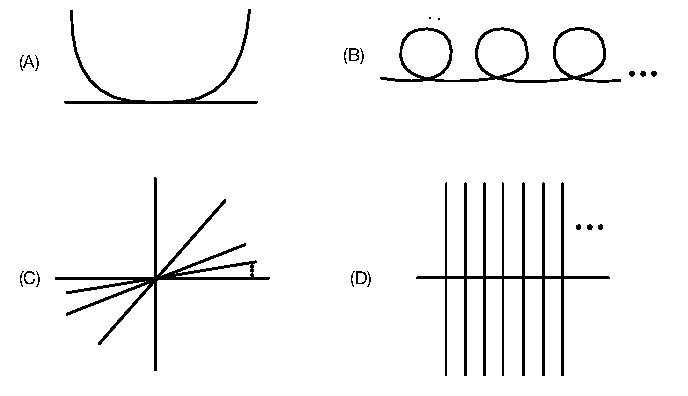
\includegraphics[width=.8\textwidth]{figures/appendix-c-artin-counterexamples.pdf}
\caption{Artin 公理的反例}\bookfigurehref{C.7.16}\label{src:C.7.16}
\end{figure}
\begin{example}[无限相切的曲线]\label{src:C.7.17}
对于图 \hyperref[src:C.7.16]{3.7.16}(A), 令 $X_q=\Spec A_q$, 其中 $A_q=\Bbbk[x,y]/(y(y-x^q))$, $A_{q+1}\to A_q$ 由 $(x,y)\mapsto(x,xy)$ 定义. 在 $F(\Bbbk[t]/t^{n+1})$ 中, 考虑由 $(x,y)\mapsto(t,0)$ 定义的元素 $\alpha_n:A_q\to\Bbbk[t]/t^{n+1}$ (对任何 $q$), 以及由 $(x,y)\mapsto(t,t^q)$ 定义的 $\beta_n:A_q\to\Bbbk[t]/t^{n+1}$ (对任何 $q$). 对每个 $n$, $\alpha_n\sim\beta_n$, 因为可取 $q\geq n+1$. 于是 $\{\alpha_n\}$ 是万有形式形变, 可有效化为两个不同的元素 $\widehat\alpha,\widehat\beta\in F(\Bbbk[\![t]\!])$, 它们在 $A_q$ (对任何 $q$) 上分别由 $\widehat\alpha(x,y)\mapsto(t,0)$ 与 $\widehat\beta(x,y)\mapsto(t,t^q)$ 定义. 因而函子 $F(\Bbbk[t])\to\varprojlim F(\Bbbk[t]/t^q)$ 不单射, 所以有效性公理 $(\mathrm{AA}_5)$ 不成立. 此时 \bookref{C.7.1}(5) (万有性的开性) 也不成立. 同样, $F$ 的对角不可表: $\underline{\Isom}_{\Bbbk[t]}(\widehat\alpha,\widehat\beta)$ 的形式形变 $\{\alpha_n\xrightarrow\sim\beta_n\}$ 无效.
\end{example}
\begin{example}[无限多个节点]\label{src:C.7.18}
对于图 \hyperref[src:C.7.16]{3.7.16}(B), 令 $X_q$ 为将 $\mathbb A^1$ 上 $q$ 对点按节点方式粘合得到的具有 $q$ 个节点的 $\mathbb C$ 上仿射概形. 则 $\mathbb A^1\to\operatorname{colim}X_q$ 在任何不映到节点的点处形式万有, 但在 $\mathbb A^1$ 的任何开邻域中都不形式万有, 因为必须去掉无限多个点. 因而 \bookref{C.7.1}(5) (万有性的开性) 不成立.

类似地, 对于图 \hyperref[src:C.7.16]{3.7.16}(C), 若 $X_q=\Spec\Bbbk[x,y]/(y\prod_{i=1}^1(x-q))$, 则包含映射 $\mathbb A^1\to\operatorname{colim}X_q$ 在任何非节点处形式万有, 但在开邻域中不形式万有.
\end{example}
\begin{example}[无限多条直线]\label{src:C.7.19}
对于图 \hyperref[src:C.7.16]{3.7.16}(D), 令 $X_q=\Spec\Bbbk[x,y]/\prod_{i=1}^q(iy-x)$ 为平面中 $q$ 条直线的并, $X_q\to X_{q+1}$ 为诱导的闭浸入. 则 $\operatorname{colim}X_q$ 满足 Schlessinger 公理 $(\mathrm H_1)$--$(\mathrm H_4)$ (等价地, Rim--Schlessinger 公理 $(\mathrm{RS}_1)$--$(\mathrm{RS}_4)$). 因而可应用 Schlessinger 定理得到形式万有形变 $\{x_n\}$, 其中 $x_n\in(\operatorname{colim}X_q)(\Bbbk[x,y]/(x,y)^{n+1})$ 由闭浸入 $\Spec\Bbbk[x,y]/(x,y)^{n+1}\to X_{n+1}$ 定义. 有效性公理 $(\mathrm{AA}_5)$ 不成立, 因为不存在延拓 $\{x_n\}$ 的 $(\operatorname{colim}X_q)(\Bbbk[x,y])$ 的元素.
\end{example}
\begin{example}[Hom 叠]\label{src:C.7.20}
若 $\mathcal X,\mathcal Y$ 在 $\Bbbk$ 上固有, 则 $(\Sch/\Bbbk)_{\text{ét}}$ 上的 Hom 叠 $\underline{\operatorname{Mor}}(\mathcal X,\mathcal Y)$ 是代数叠 (习题 \bookref{C.7.9}). 更一般地, 对任意基底, 若 $\mathcal X\to S$ 固有且平坦, 而只假设 $\mathcal Y\to S$ 局部有限表现, 拟分离且稳定子群仿射, 结论仍成立; 见 \cite[定理 $1.2$]{HR19b} 和 \cite[推论 $1.6$]{BHL17}. 在这些情形中, Tannaka 对偶 (\bookref{7.6.1}) 的一个版本成立, 即 $\operatorname{Mor}(\mathcal X,\mathcal Y)\xrightarrow\sim\operatorname{Mor}^{\otimes}(\operatorname{Coh}(\mathcal Y),\operatorname{Coh}(\mathcal X))$, 从而将有效性公理 $(\mathrm{AA}_5)$ 归结为 Grothendieck 存在性定理的一个版本.

然而, $\mathcal Y$ 具有仿射稳定子至关重要. 若 $\mathcal Y$ 为阿贝尔簇的分类叠, 则 Tannaka 对偶可能不成立, Hom 叠 $\underline{\operatorname{Mor}}(\mathcal X,\mathcal Y)$ 可能不是代数叠; 见 \cite[Tag 0AF8]{SP} 和 \cite[\S$10$]{HR19b}.
\end{example}
\begin{exercise}[光滑曲线函子的层化]\label{src:C.7.21}
设 $F$ 为函子 $S\mapsto\mathcal M_g(S)/{\sim}$ 在 $(\Sch/\Bbbk)_{\text{ét}}$ 中的层化, 其中 $\mathcal M_g(S)/{\sim}$ 为 $S$ 上光滑曲线族的同构类集合. $F$ 不满足哪一条 Artin 公理?
\end{exercise}

\clearpage
\RemoveFromHook{shipout/foreground}[appendix-c-index-pages]
\hypersetup{pageanchor=true}
\setlength{\emergencystretch}{0pt}
\appendixakeepheadingfalse
\backmatter
\begingroup
\setlength{\emergencystretch}{4em}
\printbibliography[heading=bibintoc,title={参考文献}]
\endgroup
\printindex
\end{document}
